% This LaTeX document needs to be compiled with XeLaTeX.
\documentclass[10pt]{article}
\usepackage[utf8]{inputenc}
\usepackage{amsmath}
\usepackage{amsfonts}
\usepackage{amssymb}
\usepackage[version=4]{mhchem}
\usepackage{stmaryrd}
\usepackage{graphicx}
\usepackage[export]{adjustbox}
\graphicspath{ {./images/} }
\usepackage{multirow}
\usepackage{hyperref}
\hypersetup{colorlinks=true, linkcolor=blue, filecolor=magenta, urlcolor=cyan,}
\urlstyle{same}
\usepackage[fallback]{xeCJK}
\usepackage{polyglossia}
\usepackage{fontspec}
\setCJKmainfont{Noto Serif CJK TC}

\setmainlanguage{english}
\setmainfont{CMU Serif}

\title{3.10 REFERENCES }


\author{P. R. Gray, P. J. Hurst, S. H. Lewis, and R. G. Meyer. Analysis and Design of An alog Integrated Circuits, 5th ed. John Wiley \& Sons, New York, 2009.}
\date{}


%New command to display footnote whose markers will always be hidden
\let\svthefootnote\thefootnote
\newcommand\blfootnotetext[1]{%
  \let\thefootnote\relax\footnote{#1}%
  \addtocounter{footnote}{-1}%
  \let\thefootnote\svthefootnote%
}

%Overriding the \footnotetext command to hide the marker if its value is `0`
\let\svfootnotetext\footnotetext
\renewcommand\footnotetext[2][?]{%
  \if\relax#1\relax%
    \ifnum\value{footnote}=0\blfootnotetext{#2}\else\svfootnotetext{#2}\fi%
  \else%
    \if?#1\ifnum\value{footnote}=0\blfootnotetext{#2}\else\svfootnotetext{#2}\fi%
    \else\svfootnotetext[#1]{#2}\fi%
  \fi
}

\begin{document}
\maketitle
\section*{Integrated-Circuit Devices and Modelling}
In this chapter, both the operation and modelling of semiconductor devices are described. Although it is possible to do simple integrated-circuit design with a basic knowledge of semiconductor device modelling, for state-of-theart design, an in-depth understanding of the second-order effects of device operation and their modelling is considered critical.

It is assumed that most readers have been introduced to transistors and their basic modelling in a previous course. Thus, fundamental semiconductor concepts are only briefly reviewed. Section 1.1 describes pn junctions (or diodes). This section is important in understanding the parasitic capacitances in many device models, such as junction capacitances. Section 1.2 covers the basics of MOS transistors and modelling. A summary of device models and important equations is presented in Section 1.3. This summary is particularly useful for a reader who already has a good background in transistor modelling, in which case the summary can be used to follow the notation used throughout the remainder of this book. Advanced MOS modelling is treated in Section 1.4, including behavior not covered by a simple square-law voltage-current relationship. It should be noted that all sections on MOS devices rely to some degree on the material previously presented in Section 1.1, in which depletion capacitance is covered. In addition, a brief description is given of the most important process-related parameters used in SPICE modelling in Section 1.5. Since passive devices are often required for analog design, the most common passives on integrated circuits are described in Section 1.6. Finally, this chapter concludes with an Appendix containing derivations of the more physically-based device equations.

\subsection*{1.1 SEMICONDUCTORS AND pn JUNCTIONS}
A semiconductor is a crystal lattice structure that can have free electrons (which are negative carriers) and/or free holes (which are an absence of electrons and are equivalent to positive carriers). The type of semiconductor typically used is silicon, an abundant element found, for example, in high concentrations in sand. This material has a valence of four, implying that each atom has four electrons to share with neighboring atoms when forming the covalent bonds of the crystal lattice. Intrinsic silicon (i.e., undoped silicon) is a very pure crystal structure that has equal numbers of free electrons and holes. These free carriers are those electrons that have gained enough energy due to thermal agitation to escape their bonds, and the resulting holes that they leave behind. At room temperature, there are approximately $1.1 \times 10^{10}$ carriers of each type per $\mathrm{cm}^{3}$, or equivalently $\mathrm{n}_{\mathrm{i}}=1.1 \times 10^{16}$ carriers $/ \mathrm{m}^{3}$, defined as the carrier concentration of intrinsic silicon. The number of carriers approximately doubles for every $11^{\circ} \mathrm{C}$ increase in temperature.

If one dopes silicon with a pentavalent impurity (i.e., atoms of an element having a valence of five, or equivalently five electrons in the outer shell, available when bonding with neighboring atoms), there will be almost one extra free electron for every impurity atom. ${ }^{1}$ These free electrons can be used to conduct current. A pentavalent

\footnotetext{\begin{enumerate}
  \item In fact, there will be slightly fewer mobile carriers than the number of impurity atoms since some of the free electrons from the dopants have recombined with holes. However, since the number of holes of intrinsic silicon is much less than typical doping concentrations, this inaccuracy is small.
\end{enumerate}
}
impurity is said to donate free electrons to the silicon crystal, and thus the impurity is known as a donor. Examples of donor elements are phosphorus, P , and arsenic, As. These impurities are also called n-type dopants since the free carriers resulting from their use have negative charge. When an n-type impurity is used, the total number of negative carriers or electrons is almost the same as the doping concentration, and is much greater than the number of free electrons in intrinsic silicon. In other words,\\
\$\$

\begin{equation*}
\mathrm{n}_{\mathrm{n}}=\mathrm{N}_{\mathrm{D}} \tag{1.1}
\end{equation*}

$$
where $n_{n}$ denotes the free-electron concentration in $n$-type material and $N_{D}$ is the doping concentration (with the subscript D denoting donor). On the other hand, the number of free holes in $n$-doped material will be much less than the number of holes in intrinsic silicon and can be shown [Sze, 1981] to be given by
$$

\begin{equation*}
\mathrm{p}_{\mathrm{n}}=\frac{\mathrm{n}_{\mathrm{i}}^{2}}{\mathrm{~N}_{\mathrm{D}}} \tag{1.2}
\end{equation*}

\$\$

Similarly, if one dopes silicon with atoms that have a valence of three, for example, boron (B), the concentration of positive carriers or holes will be approximately equal to the acceptor concentration, $\mathrm{N}_{\mathrm{A}}$,


\begin{equation*}
\mathrm{p}_{\mathrm{p}}=\mathrm{N}_{\mathrm{A}} \tag{1.3}
\end{equation*}


and the number of negative carriers in the p -type silicon, $\mathrm{n}_{\mathrm{p}}$, is given by


\begin{equation*}
\mathrm{n}_{\mathrm{p}}=\frac{\mathrm{n}_{\mathrm{i}}^{2}}{\mathrm{~N}_{\mathrm{A}}} \tag{1.4}
\end{equation*}


\section*{EXAMPLE 1.1}
Intrinsic silicon is doped with boron at a concentration of $10^{26}$ atoms $/ \mathrm{m}^{3}$. At room temperature, what are the concentrations of holes and electrons in the resulting doped silicon? Assume that $\mathrm{n}_{\mathrm{i}}=1.1 \times 10^{16}$ carriers $/ \mathrm{m}^{3}$.

\section*{Solution}
The hole concentration, $p_{p}$, will approximately equal the doping concentration $\left(p_{p}=N_{A}=10^{26}\right.$ holes $\left./ \mathrm{m}^{3}\right)$. The electron concentration is found from (1.4) to be


\begin{equation*}
\mathrm{n}_{\mathrm{p}}=\frac{\left(1.1 \times 10^{16}\right)^{2}}{10^{26}}=1.2 \times 10^{6} \text { electrons } / \mathrm{m}^{3} \tag{1.5}
\end{equation*}


Such doped silicon is referred to as p-type since it has many more free holes than free electrons.

\subsection*{1.1.1 Diodes}
To realize a diode, also called a pn junction, one part of a semiconductor is doped $n$-type and an adjacent part is doped p -type, as shown in Fig. 1.1. The diode, or junction, is formed between the $\mathrm{p}^{+}$region and the n region, where superscripts are used to indicate the relative doping levels. For example, the $\mathrm{p}^{-}$bulk region in Fig. 1.1 might have an impurity concentration of $5 \times 10^{21}$ carriers $/ \mathrm{m}^{3}$, whereas the $\mathrm{p}^{+}$and $\mathrm{n}^{+}$regions would be doped more\\
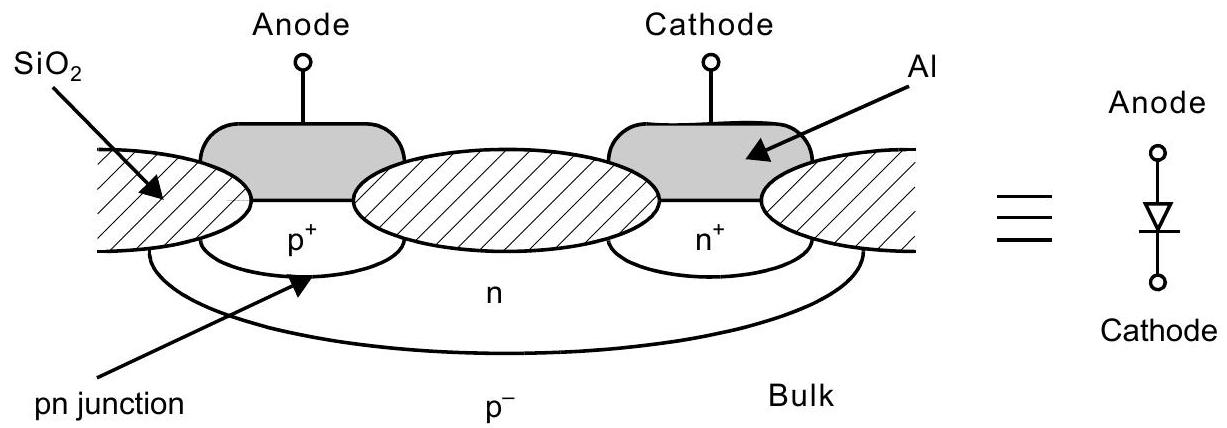
\includegraphics[max width=\textwidth, center]{2024_10_31_60860e27b87166db2267g-027}

Fig. 1.1 A cross section of a pn diode.\\
heavily to a value around $10^{25}$ to $10^{27}$ carriers $/ \mathrm{m}^{3}{ }^{2}$ Also, note that the metal contacts to the diode (in this case, aluminum) are connected to heavily doped regions, otherwise a Schottky diode would form. (Schottky diodes are discussed on page 13.) Thus, in order not to make a Schottky diode, the connection to the n region is actually made via the $\mathrm{n}^{+}$region.

In the $\mathrm{p}^{+}$side, a large number of free positive carriers are available, whereas in the n side, many free negative carriers are available. The holes in the $\mathrm{p}^{+}$side will tend to disperse or diffuse into the n side, whereas the free electrons in the n side will tend to diffuse to the $\mathrm{p}^{+}$side. This process is very similar to two gases randomly diffusing together. This diffusion lowers the concentration of free carriers in the region between the two sides. As the two types of carriers diffuse together, they recombine. Every electron that diffuses from the n side to the p side leaves behind a bound positive charge close to the transition region. Similarly, every hole that diffuses from the p side leaves behind a bound electron near the transition region. The end result is shown in Fig. 1.2. This diffusion of free carriers creates a depletion region at the junction of the two sides where no free carriers exist, and which has a net negative charge on the $\mathrm{p}^{+}$side and a net positive charge on the n side. The total amount of exposed or bound charge on the two sides of the junction must be equal for charge neutrality. This requirement causes the depletion region to extend farther into the more lightly doped n side than into the $\mathrm{p}^{+}$side.

As these bound charges are exposed, an electric field develops going from the n side to the $\mathrm{p}^{+}$side. This electric field gives rise to a potential difference between the n and $\mathrm{p}^{+}$sides, called the built-in voltage of the junction. It opposes the diffusion of free carriers until there is no net movement of charge under open-circuit and steadystate conditions. The built-in voltage of an open-circuit pn junction is [Sze 1981]


\begin{equation*}
\Phi_{0}=\mathrm{V}_{\mathrm{T}} \ln \left(\frac{\mathrm{~N}_{\mathrm{A}} \mathrm{~N}_{\mathrm{D}}}{\mathrm{n}_{\mathrm{i}}^{2}}\right) \tag{1.6}
\end{equation*}


where


\begin{equation*}
V_{T}=\frac{k T}{q} \tag{1.7}
\end{equation*}


T is the temperature in degrees Kelvin ( $\cong 300^{\circ} \mathrm{K}$ at room temperature), k is Boltzmann's constant $\left(1.38 \times 10^{-23} \mathrm{JK}^{-1}\right)$, and q is the charge of an electron $\left(1.602 \times 10^{-19} \mathrm{C}\right)$. At room temperature, $\mathrm{V}_{\mathrm{T}}$ is approximately 26 mV .

\section*{EXAMPLE 1.2}
A pn junction has $\mathrm{N}_{\mathrm{A}}=10^{25}$ holes $/ \mathrm{m}^{3}$ and $\mathrm{N}_{\mathrm{D}}=10^{22}$ electrons $/ \mathrm{m}^{3}$. What is the built-in junction potential? Assume that $\mathrm{n}_{\mathrm{i}}=1.1 \times 10^{16}$ carriers $/ \mathrm{m}^{3}$.

\section*{Solution}
Using (1.6), we obtain


\begin{equation*}
\Phi_{0}=0.026 \times \ln \left(\frac{10^{25} \times 10^{22}}{\left(1.1 \times 10^{16}\right)^{2}}\right)=0.89 \mathrm{~V} \tag{1.8}
\end{equation*}


This is a typical value for the built-in potential of a junction with one side heavily doped. As an approximation, we will normally use $\Phi_{0} \cong 0.9 \mathrm{~V}$ for the built-in potential of a junction having one side heavily doped.

\subsection*{1.1.2 Reverse-Biased Diodes}
A silicon diode having an anode-to-cathode (i.e., p side to n side) voltage of 0.4 V or less will not be conducting appreciable current. In this case, it is said to be reverse-biased. If a diode is reverse-biased, current flow is primarily due to thermally generated carriers in the depletion region, and it is extremely small. Although this reverse-biased current is only weakly dependent on the applied voltage, the reverse-biased current is directly proportional to the area of the diode junction. However, an effect that should not be ignored, particularly at high frequencies, is the junction capacitance of a diode. In reverse-biased diodes, this junction capacitance is due to varying charge storage in the depletion regions and is modelled as a depletion capacitance.

To determine the depletion capacitance, we first state the relationship between the depletion widths and the applied reverse voltage, $\mathrm{V}_{\mathrm{R}}$ [Sze, 1981].


\begin{align*}
& x_{n}=\left[\frac{2 \mathrm{~K}_{\mathrm{s}} \varepsilon_{0}\left(\Phi_{0}+\mathrm{V}_{\mathrm{R}}\right)}{\mathrm{q}} \frac{\mathrm{~N}_{\mathrm{A}}}{\mathrm{~N}_{\mathrm{D}}\left(\mathrm{~N}_{\mathrm{A}}+\mathrm{N}_{\mathrm{D}}\right)}\right]^{1 / 2}  \tag{1.9}\\
& \mathrm{x}_{\mathrm{p}}=\left[\frac{2 \mathrm{~K}_{\mathrm{s}} \varepsilon_{0}\left(\Phi_{0}+\mathrm{V}_{\mathrm{R}}\right)}{\mathrm{q}} \frac{\mathrm{~N}_{\mathrm{D}}}{\mathrm{~N}_{\mathrm{A}}\left(\mathrm{~N}_{\mathrm{A}}+\mathrm{N}_{\mathrm{D}}\right)}\right]^{1 / 2} \tag{1.10}
\end{align*}


Here, $\varepsilon_{0}$ is the permittivity of free space (equal to $8.854 \times 10^{-12} \mathrm{~F} / \mathrm{m}$ ), $\mathrm{V}_{\mathrm{R}}$ is the reverse-bias voltage of the diode, and $\mathrm{K}_{\mathrm{s}}$ is the relative permittivity of silicon (equal to 11.8). These equations assume an abrupt junction where the doping changes instantly from the n to the p side. Modifications to these equations for graded junctions are treated in the next section.

From the above equations, we see that if one side of the junction is more heavily doped than the other, the depletion region will extend mostly on the lightly doped side. For example, if $N_{A} \gg N_{D}$ (i.e., if the $p$ region is more heavily doped), we can approximate (1.9) and (1.10) as


\begin{equation*}
\mathrm{x}_{\mathrm{n}} \cong\left[\frac{2 \mathrm{~K}_{\mathrm{s}} \varepsilon_{0}\left(\Phi_{0}+\mathrm{V}_{\mathrm{R}}\right)}{\mathrm{qN}}\right]^{1 / 2} \mathrm{x}_{\mathrm{p}} \cong\left[\frac{2 \mathrm{~K}_{\mathrm{s}} \varepsilon_{0}\left(\Phi_{0}+\mathrm{V}_{\mathrm{R}}\right) \mathrm{N}_{\mathrm{D}}}{q N_{A}^{2}}\right]^{1 / 2} \tag{1.11}
\end{equation*}


Indeed, for this case


\begin{equation*}
\frac{x_{n}}{x_{p}} \cong \frac{N_{A}}{N_{D}} \tag{1.12}
\end{equation*}


This special case is called a single-sided diode.

\section*{EXAMPLE 1.3}
For a pn junction having $\mathrm{N}_{\mathrm{A}}=10^{25}$ holes $/ \mathrm{m}^{3}$ and $\mathrm{N}_{\mathrm{D}}=10^{22}$ electrons $/ \mathrm{m}^{3}$, what are the depletion region depths for a $1-\mathrm{V}$ reverse-bias voltage?

\section*{Solution}
Since $\mathrm{N}_{\mathrm{A}} \gg>\mathrm{N}_{\mathrm{D}}$ and we already have found in Example 1.2 that $\Phi_{0}=0.9 \mathrm{~V}$, we can use (1.11) to find


\begin{gather*}
\mathrm{x}_{\mathrm{n}}=\left[\frac{2 \times 11.8 \times 8.854 \times 10^{-12} \times 1.9}{1.6 \times 10^{-19} \times 10^{22}}\right]^{1 / 2}=0.50 \mu \mathrm{~m}  \tag{1.13}\\
\mathrm{x}_{\mathrm{p}}=\frac{\mathrm{x}_{\mathrm{n}}}{\left(\mathrm{~N}_{\mathrm{A}} / \mathrm{N}_{\mathrm{D}}\right)}=0.50 \mathrm{~nm} \tag{1.14}
\end{gather*}


Note that the depletion region width in the lightly doped n region is 1,000 times greater than that in the more heavily doped $p$ region.

The charge stored in the depletion region, per unit cross-sectional area, is found by multiplying the depletion region width by the concentration of the immobile charge (which is approximately equal to q times the impurity doping density). For example, on the n side, we find the charge in the depletion region to be given by multiplying (1.9) by $\mathrm{qN}_{\mathrm{D}}$, resulting in


\begin{equation*}
\mathrm{Q}^{+}=\left[2 \mathrm{qK}_{\mathrm{s}} \varepsilon_{0}\left(\Phi_{0}+\mathrm{V}_{\mathrm{R}}\right) \frac{\mathrm{N}_{\mathrm{A}} \mathrm{~N}_{\mathrm{D}}}{\mathrm{~N}_{\mathrm{A}}+\mathrm{N}_{\mathrm{D}}}\right]^{1 / 2} \tag{1.15}
\end{equation*}


This amount of charge must also equal $\mathrm{Q}^{-}$on the p side since there is charge equality. In the case of a single-sided diode when $N_{A} \gg N_{D}$, we have


\begin{equation*}
\mathrm{Q}^{-}=\mathrm{Q}^{+} \cong\left[2 \mathrm{qK}_{\mathrm{s}} \varepsilon_{0}\left(\Phi_{0}+\mathrm{V}_{\mathrm{R}}\right) \mathrm{N}_{\mathrm{D}}\right]^{1 / 2} \tag{1.16}
\end{equation*}


Key Point: The chargevoltage relationship of a reverse-biased pn junction is modeled by a nonlinear depletion capacitance.

Note that this result is independent of the impurity concentration on the heavily doped side. Thus, we see from the above relation that the charge stored in the depletion region is nonlinearly dependent on the applied reverse-bias voltage. This charge-voltage relationship is modelled by a nonlinear depletion capacitance.

For small changes in the reverse-biased junction voltage, about a bias voltage, we can find an equivalent small-signal capacitance, $\mathrm{C}_{\mathrm{j}}$, by differentiating (1.15) with respect to $\mathrm{V}_{\mathrm{R}}$. Such a differentiation results in


\begin{equation*}
C_{j}=\frac{\mathrm{dQ}^{+}}{d V_{R}}=\left[\frac{q K_{s} \varepsilon_{0}}{2\left(\Phi_{0}+V_{R}\right)} \frac{N_{A} N_{D}}{N_{A}+N_{D}}\right]^{1 / 2}=\frac{C_{j 0}}{\sqrt{1+\frac{V_{B}}{\Phi_{0}}}} \tag{1.17}
\end{equation*}


where $C_{j 0}$ is the depletion capacitance per unit area at $V_{R}=0$ and is given by


\begin{equation*}
C_{j} 0=\sqrt{\frac{q K_{s} \varepsilon_{0}}{2 \Phi_{0}} \frac{N_{A} N_{D}}{N_{A}+N_{D}}} \tag{1.18}
\end{equation*}


In the case of a one-sided diode with $\mathrm{N}_{\mathrm{A}} \gg \mathrm{N}_{\mathrm{D}}$, we have


\begin{equation*}
\mathrm{C}_{\mathrm{j}}=\left[\frac{\mathrm{qK}_{\mathrm{s}} \varepsilon_{0} \mathrm{~N}_{\mathrm{D}}}{2\left(\Phi_{0}+\mathrm{V}_{\mathrm{R}}\right)}\right]^{1 / 2}=\frac{\mathrm{C}_{\mathrm{j} 0}}{\sqrt{1+\frac{\mathrm{V}_{\mathrm{R}}}{\Phi_{0}}}} \tag{1.19}
\end{equation*}


where now


\begin{equation*}
C_{j 0}=\sqrt{\frac{q K_{s} \varepsilon_{0} N_{D}}{2 \Phi_{0}}} \tag{1.20}
\end{equation*}


It should be noted that many of the junctions encountered in integrated circuits are one-sided junctions with the lightly doped side being the substrate or sometimes what is called the well. The more heavily doped side is often used to form a contact to interconnecting metal. From (1.20), we see that, for these one-sided junctions, the depletion capacitance is approximately independent of the doping concentration on the heavily doped side, and is proportional to the square root of the doping concentration of the more lightly doped side. Thus, smaller depletion capacitances are obtained for more lightly doped substrates - a strong incentive to strive for lightly doped substrates.

Finally, note that by combining (1.15) and (1.18), we can express the equation for the immobile charge on either side of a reverse-biased junction as


\begin{equation*}
\mathrm{Q}=2 \mathrm{C}_{\mathrm{j} 0} \Phi_{0} \sqrt{1+\frac{\mathrm{V}_{\mathrm{R}}}{\Phi_{0}}} \tag{1.21}
\end{equation*}


As seen in Example 1.6, this equation is useful when one is approximating the large-signal charging (or discharging) time for a reverse-biased diode.

\section*{EXAMPLE 1.4}
For a pn junction having $\mathrm{N}_{\mathrm{A}}=10^{25}$ holes $/ \mathrm{m}^{3}$ and $\mathrm{N}_{\mathrm{D}}=10^{22}$ electrons $/ \mathrm{m}^{3}$, what is the total zero-bias depletion capacitance for a diode of area $10 \mu \mathrm{~m} \times 10 \mu \mathrm{~m}$ ? What is its depletion capacitance for a 3-V reverse-bias voltage?

\section*{Solution}
Making use of (1.20), we have


\begin{equation*}
C_{j 0}=\sqrt{\frac{1.6 \times 10^{-19} \times 11.8 \times 8.854 \times 10^{-12} \times 10^{22}}{2 \times 0.9}}=304.7 \mu \mathrm{~F} / \mathrm{m}^{2} \tag{1.22}
\end{equation*}


Since the diode area is $100 \times 10^{-12} \mathrm{~m}^{2}$, the total zero-bias depletion capacitance is


\begin{equation*}
\mathrm{C}_{\mathrm{T}-\mathrm{j} 0}=100 \times 10^{-12} \times 304.7 \times 10^{-6}=30.5 \mathrm{fF} \tag{1.23}
\end{equation*}


At a 3-V reverse-bias voltage, we have from (1.19)


\begin{equation*}
\mathrm{C}_{\mathrm{T}-\mathrm{j}}=\frac{30.5 \mathrm{fF}}{\sqrt{1+\left(\frac{3}{0.9}\right)}}=14.7 \mathrm{fF} \tag{1.24}
\end{equation*}


We see a decrease in junction capacitance as the width of the depletion region is increased.

\subsection*{1.1.3 Graded Junctions}
All of the above equations assumed an abrupt junction where the doping concentration changes quickly from p to n over a small distance. Although this is a good approximation for many integrated circuits, it is not always so. For example, the collector-to-base junction of a bipolar transistor is most commonly realized as a graded junction. In the case of graded junctions, the exponent $1 / 2$ in (1.15) is inaccurate, and an exponent closer to unity is more accurate, perhaps 0.6 to 0.7 . Thus, for graded junctions, (1.15) is typically written as


\begin{equation*}
Q=\left[2 q K_{s} \varepsilon_{0}\left(\Phi_{0}+V_{R}\right) \frac{N_{A} N_{D}}{N_{A}+N_{D}}\right]^{1-m_{j}} \tag{1.25}
\end{equation*}


where $m_{j}$ is a constant that depends upon the doping profile. For example, a linearly graded junction has $m_{j}=1 / 3$.\\
Differentiating (1.25) to find the depletion capacitance, we have


\begin{equation*}
C_{j}=\left(1-m_{j}\right)\left[2 q K_{s} \varepsilon_{0} \frac{N_{A} N_{D}}{N_{A}+N_{D}}\right]^{1-m_{j}} \frac{1}{\left(\Phi_{0}+V_{R}\right)^{m_{j}}} \tag{1.26}
\end{equation*}


This depletion capacitance can also be written as


\begin{equation*}
C_{j}=\frac{C_{j 0}}{\left(1+\frac{V_{R}}{\Phi_{0}}\right)^{m_{j}}} \tag{1.27}
\end{equation*}


where


\begin{equation*}
C_{j 0}=\left(1-m_{j}\right)\left[2 q K_{s} \varepsilon_{0} \frac{N_{A} N_{D}}{N_{A}+N_{D}}\right]^{1-m_{j}} \frac{1}{\Phi_{0}^{m_{j}}} \tag{1.28}
\end{equation*}


From (1.27), we see that a graded junction results in a depletion capacitance that is less dependent on $\mathrm{V}_{\mathrm{R}}$ than the equivalent capacitance in an abrupt junction. In other words, since $m$ is less than 0.5 , the depletion capacitance for a graded junction is more linear than that for an abrupt junction. Correspondingly, increasing the reverse-bias voltage for a graded junction is not as effective in reducing the depletion capacitance as it is for an abrupt junction.

Finally, as in the case of an abrupt junction, the depletion charge on either side of the junction can also be written as


\begin{equation*}
\mathrm{Q}=\frac{\mathrm{C}_{\mathrm{j} 0}}{1-\mathrm{m}_{\mathrm{j}}} \Phi_{0}\left(1+\frac{\mathrm{V}_{\mathrm{R}}}{\Phi_{0}}\right)^{1-\mathrm{m}_{\mathrm{j}}} \tag{1.29}
\end{equation*}


\section*{EXAMPLE 1.5}
Repeat Example 1.4 for a graded junction with $\mathrm{m}_{\mathrm{j}}=0.4$.

\section*{Solution}
Noting once again that $\mathrm{N}_{\mathrm{A}} \gg \mathrm{N}_{\mathrm{D}}$, we approximate (1.28) as


\begin{equation*}
\mathrm{C}_{\mathrm{j} 0}=\left(1-\mathrm{m}_{\mathrm{j}}\right)\left[2 \mathrm{qK}_{\mathrm{s}} \varepsilon_{0} \mathrm{~N}_{\mathrm{D}}\right]^{1-\mathrm{m}_{\mathrm{j}}} \frac{1}{\Phi_{0}^{m_{\mathrm{j}}}} \tag{1.30}
\end{equation*}


resulting in


\begin{equation*}
\mathrm{C}_{\mathrm{j} 0}=81.5 \mu \mathrm{~F} / \mathrm{m}^{2} \tag{1.31}
\end{equation*}


which, when multiplied by the diode's area of $10 \mu \mathrm{~m} \times 10 \mu \mathrm{~m}$, results in


\begin{equation*}
\mathrm{C}_{\mathrm{T}-\mathrm{j} 0}=8.1 \mathrm{fF} \tag{1.32}
\end{equation*}


For a 3-V reverse-bias voltage, we have


\begin{equation*}
\mathrm{C}_{\mathrm{T}-\mathrm{j}}=\frac{8.1 \mathrm{fF}}{(1+3 / 0.9)^{0.4}}=4.5 \mathrm{fF} \tag{1.33}
\end{equation*}


\subsection*{1.1.4 Large-Signal Junction Capacitance}
The equations for the junction capacitance given above are only valid for small changes in the reverse-bias voltage. This limitation is due to the fact that $\mathrm{C}_{\mathrm{j}}$ depends on the size of the reverse-bias voltage instead of being a constant. As a result, it is extremely difficult and time consuming to accurately take this nonlinear capacitance into account when calculating the time to charge or discharge a junction over a large voltage change. A commonly used approximation when analyzing the transient response for large voltage changes is to use an average size for the junction capacitance by calculating the junction capacitance at the two extremes of the reverse-bias voltage. Unfortunately, a problem with this approach is that when the diode is forward biased with $\mathrm{V}_{\mathrm{R}} \cong-\Phi_{0}$, equation (1.17) "blows up" (i.e., is equal to infinity). To circumvent this problem, one can instead calculate the charge stored in the junction for the two extreme values of applied voltage (through the use of (1.21)), and then through the use of $\mathrm{Q}=\mathrm{CV}$, calculate the average capacitance according to


\begin{equation*}
C_{j-\mathrm{av}}=\frac{Q\left(V_{2}\right)-Q\left(V_{1}\right)}{V_{2}-V_{1}} \tag{1.34}
\end{equation*}


where $\mathrm{V}_{1}$ and $\mathrm{V}_{2}$ are the two voltage extremes [Hodges, 1988].\\
From (1.21), for an abrupt junction with reverse-bias voltage $V_{i}$, we have


\begin{equation*}
\mathrm{Q}\left(\mathrm{~V}_{\mathrm{i}}\right)=2 \mathrm{C}_{\mathrm{j} 0} \Phi_{0} \sqrt{1+\frac{\mathrm{V}_{\mathrm{i}}}{\Phi_{0}}} \tag{1.35}
\end{equation*}


Therefore,


\begin{equation*}
\mathrm{C}_{\mathrm{j}-\mathrm{av}}=2 \mathrm{C}_{\mathrm{j} 0} \Phi_{0} \frac{\left(\sqrt{1+\frac{\mathrm{V}_{2}}{\Phi_{0}}}-\sqrt{1+\frac{\mathrm{V}_{1}}{\Phi_{0}}}\right)}{\mathrm{V}_{2}-\mathrm{V}_{1}} \tag{1.36}
\end{equation*}


\section*{EXAMPLE 1.6}
For the circuit shown in Fig. 1.3, where a reverse-biased diode is being charged from 0 V to 1 V , through a $10-\mathrm{k} \Omega$ resistor, calculate the time required to charge the diode from 0 V to 0.7 V . Assume that $\mathrm{C}_{\mathrm{j} 0}=0.2 \mathrm{fF} /(\mu \mathrm{m})^{2}$ and that the diode has an area of $20 \mu \mathrm{~m} \times 5 \mu \mathrm{~m}$. Compare your answer to that obtained using SPICE. Repeat the question for the case of the diode being discharged from 1 V to 0.3 V .

\section*{Solution}
For the special case of $\mathrm{V}_{1}=0 \mathrm{~V}$ and $\mathrm{V}_{2}=1 \mathrm{~V}$, and using $\Phi_{0}=0.9 \mathrm{~V}$ in equation (1.36) we find that


\begin{equation*}
C_{j-a v}=0.815 C_{j 0} \tag{1.37}
\end{equation*}


Thus, as a rough approximation to quickly estimate the charging time of a junction capacitance from 0 V to 1 V (or vice versa), one can use


\begin{equation*}
C_{j-a v} \cong 0.8 C_{j 0} \tag{1.38}
\end{equation*}


The total small-signal capacitance of the junction at $0-\mathrm{V}$ bias voltage is obtained by multiplying $0.2 \mathrm{fF} /(\mu \mathrm{m})^{2}$ by the junction area to obtain


\begin{equation*}
C_{T-j 0}=0.2 \times 10^{-15} \times 20 \times 5=0.02 \mathrm{pF} \tag{1.39}
\end{equation*}


Fig. 1.3 (a) The circuit used in\\
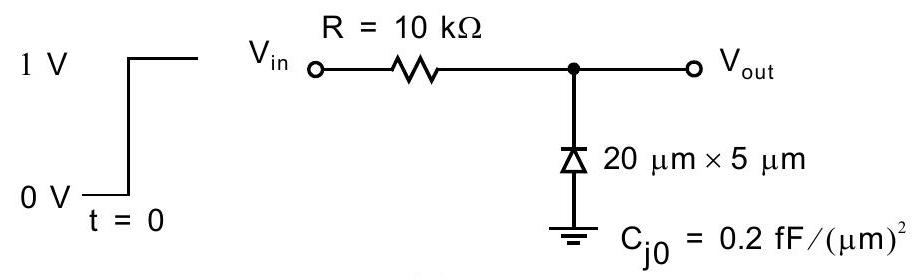
\includegraphics[max width=\textwidth, center]{2024_10_31_60860e27b87166db2267g-034}\\
(a)\\
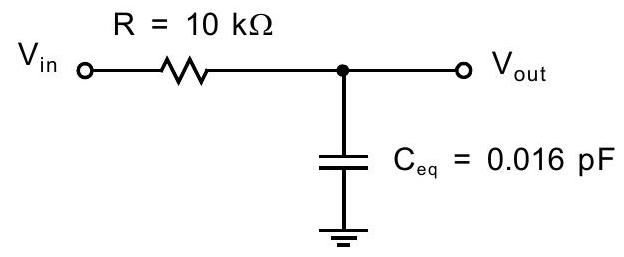
\includegraphics[max width=\textwidth, center]{2024_10_31_60860e27b87166db2267g-034(1)}

Example 1.6; (b) its RC approximate equivalent.\\
(b)

Using (1.37), we have


\begin{equation*}
\mathrm{C}_{\mathrm{T}-\mathrm{j}-\mathrm{av}}=0.815 \times 0.02=0.016 \mathrm{pF} \tag{1.40}
\end{equation*}


resulting in a time constant of


\begin{equation*}
\tau=R C_{j-a v}=0.16 \mathrm{~ns} \tag{1.41}
\end{equation*}


It is not difficult to show that the time it takes for a first-order circuit to rise (or fall) 70 percent of its final value is equal to $1.2 \tau$. Thus, in this case,


\begin{equation*}
\mathrm{t}_{70 \%}=1.2 \tau=0.20 \mathrm{~ns} \tag{1.42}
\end{equation*}


\begin{center}

\includegraphics[max width=\textwidth]{2024_10_31_60860e27b87166db2267g-034(2)}
\end{center}

As a check, the circuit of Fig. 1.3(a) was analyzed using SPICE. The SPICE simulation gave a $0-\mathrm{V}$ to $0.7-\mathrm{V}$ rise time of 0.21 ns and a $1-\mathrm{V}$ to $0.3-\mathrm{V}$ fall time of 0.19 ns , in general agreement with the 0.20 ns predicted. The reason for the different values of the rise and fall times is the nonlinearity of the junction capacitance. For smaller bias voltages it is larger than that predicted by (1.37), whereas for larger bias voltages it is smaller. Normally, the extra accuracy that results from performing a more accurate analysis is not worth the extra complication because one seldom knows the value of $\mathrm{C}_{\mathrm{j} 0}$ to better than 20 percent accuracy.

\subsection*{1.1.5 Forward-Biased Junctions}
A positive voltage applied from the p side to the n side of a diode reduces the electric field opposing the diffusion of the free carriers across the depletion region. It also reduces the width of the depletion region. If this forward-bias voltage is large enough, the carriers will start to diffuse across the junction, resulting in a current flow from the anode to the cathode. For silicon, appreciable diode current starts to occur for a forward-bias\\
voltage around 0.5 V . For germanium and gallium arsenide semiconductor materials, current conduction starts to occur around 0.3 V and 0.9 V , respectively.

When the junction potential is sufficiently lowered for conduction to occur, the carriers diffuse across the junction due to the large gradient in the mobile carrier concentrations. Note that there are more carriers diffusing from the heavily doped side to the lightly doped side than from the lightly doped side to the heavily doped side.

After the carriers cross the depletion region, they greatly increase the minority charge at the edge of the depletion region. These minority carriers will diffuse away from the junction toward the bulk. As they diffuse, they recombine with the majority carriers, thereby decreasing their concentration. This concentration gradient of the minority charge (which decreases the farther one gets from the junction) is responsible for the current flow near the junction.

The majority carriers that recombine with the diffusing minority carriers come from the metal contacts at the junctions because of the forward-bias voltage. These majority carriers flow across the bulk, from the contacts to the junction, due to an electric field applied across the bulk. This current flow is called drift. It results in small potential drops across the bulk, especially in the lightly doped side. Typical values of this voltage drop might be 50 mV to 0.1 V , depending primarily on the doping concentration of the lightly doped side, the distance from the contacts to the junction, and the cross-sectional area of the junction.

In the forward-bias region, the current-voltage relationship is exponential and can be shown (see Appendix) to be


\begin{equation*}
I_{D}=I_{S} e^{V_{D} V_{T}} \tag{1.43}
\end{equation*}


where $\mathrm{V}_{\mathrm{D}}$ is the voltage applied across the diode and


\begin{equation*}
I_{S} \propto A_{D}\left(\frac{1}{N_{A}}+\frac{1}{N_{D}}\right) \tag{1.44}
\end{equation*}


$I_{S}$ is known as the scale current and is seen to be proportional to the area of the diode junction, $A_{D}$, and inversely proportional to the doping concentrations.

\subsection*{1.1.6 Junction Capacitance of Forward-Biased Diode}
When a junction changes from reverse biased (with little current through it) to forward biased (with significant current flow across it), the charge being stored near and across the junction changes. Part of the change in charge is due to the change in the width of the depletion region and therefore the amount of immobile charge stored in it. This change in charge is modelled by the depletion capacitance, $C_{j}$, similar to when the junction is reverse biased. An additional change in charge storage is necessary to account for the change of the minority carrier concentration close to the junction required for the diffusion current to exist. For example, if a forward-biased diode current is to double, then the slopes of the minority charge storage at the diode junction edges must double, and this, in turn, implies that the minority charge storage must double. This component is modelled by another capacitance, called the diffusion capacitance, and denoted $\mathrm{C}_{\mathrm{d}}$.

The diffusion capacitance can be shown (see Appendix) to be


\begin{equation*}
\mathrm{C}_{\mathrm{d}}=\tau_{\mathrm{T}} \frac{\mathrm{I}_{\mathrm{D}}}{\mathrm{~V}_{\mathrm{T}}} \tag{1.45}
\end{equation*}


where $\tau_{\top}$ is the transit time of the diode. Normally $\tau_{\top}$ is specified for a given technology, so that one can calculate the diffusion capacitance. Note that the diffusion capac itance of a forward-biased junction is proportional to the diode current.

The total capacitance of the forward-biased junction is the sum of the diffusion capacitance, $\mathrm{C}_{\mathrm{d}}$, and the depletion capacitance, $\mathrm{C}_{\mathrm{j}}$. Thus, the total junction capacitance is given by


\begin{equation*}
C_{T}=C_{d}+C_{j} \tag{1.46}
\end{equation*}


For a forward-biased junction, the depletion capacitance, $C_{j}$, can be roughly approximated by $2 C_{j 0}$. The accuracy of this approximation is not critical since the diffusion capacitance is typically much larger than the depletion capacitance.

Finally, it should be mentioned that as a diode is turned off for a short period of time a current will flow in the negative direction until the minority charge is removed. This behavior does not occur in Schottky diodes since they do not have minority charge storage.

\subsection*{1.1.7 Small-Signal Model of a Forward-Biased Diode}
\begin{center}
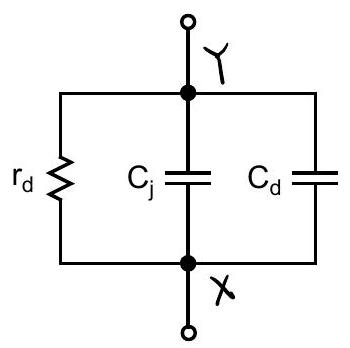
\includegraphics[max width=\textwidth]{2024_10_31_60860e27b87166db2267g-036}
\end{center}

Fig. 1.4 The small-signal model for a forward-biased junction.

A small-signal equivalent model for a forward-biased diode is shown in Fig. 1.4. A resistor, $r_{d}$, models the change in the diode voltage, $\mathrm{V}_{\mathrm{D}}$, that occurs when $I_{D}$ changes. Using (1.43), we have


\begin{equation*}
\frac{1}{r_{d}}=\frac{d I_{D}}{d V_{D}}=I_{S} \frac{e^{V_{D} / V_{T}}}{V_{T}}=\frac{I_{D}}{V_{T}} \tag{1.47}
\end{equation*}


This resistance is called the incremental resistance of the diode. For very accurate modelling, it is sometimes necessary to add the series resistance due to the bulk and also the resistance associated with the contacts. Typical values for the contact resistance (caused by the workfunction ${ }^{3}$ difference between metal and silicon) might be $20 \Omega$ to $40 \Omega$.

By combining (1.45) and (1.47), we see that an alternative equation for the diffusion capacitance, $\mathrm{C}_{\mathrm{d}}$, is


\begin{equation*}
\mathrm{C}_{\mathrm{d}}=\frac{\tau_{\mathrm{T}}}{\mathrm{r}_{\mathrm{d}}} \tag{1.48}
\end{equation*}


Since for moderate forward-bias currents, $C_{d} \gg C_{j}$, the total small-signal capacitance is $C_{T} \cong C_{d}$, and


\begin{equation*}
r_{d} C_{T} \cong \tau_{T} \tag{1.49}
\end{equation*}


Thus, for charging or discharging a forward-biased junction with a current source having an impedance much larger than $r_{d}$, the time constant of the charging is approximately equal to the transit time of the diode and is independent of the diode current. For smaller diode currents, where $\mathrm{C}_{\mathrm{j}}$ becomes important, the charging or discharging time constant of the circuit becomes larger than $\tau_{\mathrm{T}}$.

\section*{EXAMPLE 1.7}
A given diode has a transit time of 100 ps and is biased at 1 mA . What are the values of its small-signal resistance and diffusion capacitance? Assume room temperature, so that $V_{T}=k T / q=26 \mathrm{mV}$.\\
3. The work-function of a material is defined as the minimum energy required to remove an electron at the Fermi level to the outside vacuum region.

\section*{Solution}
We have

$$
\mathrm{r}_{\mathrm{d}}=\frac{\mathrm{V}_{\mathrm{T}}}{\mathrm{I}_{\mathrm{D}}}=\frac{26 \mathrm{mV}}{1 \mathrm{~mA}}=26 \Omega
$$

and

$$
\mathrm{C}_{\mathrm{d}}=\frac{\tau_{\mathrm{T}}}{\mathrm{r}_{\mathrm{d}}}=\frac{100 \mathrm{ps}}{26 \Omega}=3.8 \mathrm{pF}
$$

Note that this diffusion capacitance is over 100 times larger than the total depletion capacitance found in Examples 1.4 and 1.5 .

\subsection*{1.1.8 Schottky Diodes}
A different type of diode, one sometimes used in microcircuit design, is realized by contacting metal to a lightly doped semiconductor region (rather than a heavily doped region) as shown in Fig. 1.5. Notice that the aluminum anode is in direct contact with a relatively lightly doped $\mathrm{n}^{-}$region. Because the $\mathrm{n}^{-}$region is relatively lightly doped, the work-function difference between the aluminum contact and the $\mathrm{n}^{-}$silicon is larger than would be the case for aluminum contacting to an $\mathrm{n}^{+}$region, as occurs at the cathode. This causes a depletion region and, correspondingly, a diode to occur at the interface between the aluminum anode and the $\mathrm{n}^{-}$silicon region. This diode has different characteristics than a normal pn junction diode. First, its voltage drop when forward biased is smaller. This voltage drop is dependent on the metal used; for aluminum it might be around 0.5 V . More importantly, when the diode is forward biased, there is no minority-charge storage in the lightly doped $\mathrm{n}^{-}$region. Thus, the small-signal model of a forward-biased Schottky diode has $\mathrm{C}_{\mathrm{d}}=0$ (with reference to Fig. 1.4). The absence of this diffusion capacitance makes the diode much faster. It is particularly faster when turning off, because it is not necessary to remove the minority charge first. Rather, it is only necessary to discharge the depletion capacitance through about 0.2 V .

Schottky diodes have been used extensively in bipolar logic circuits. They are also used in a number of highspeed analog circuits, particularly those realized in gallium arsenide (GaAs) technologies, rather than silicon technologies.\\
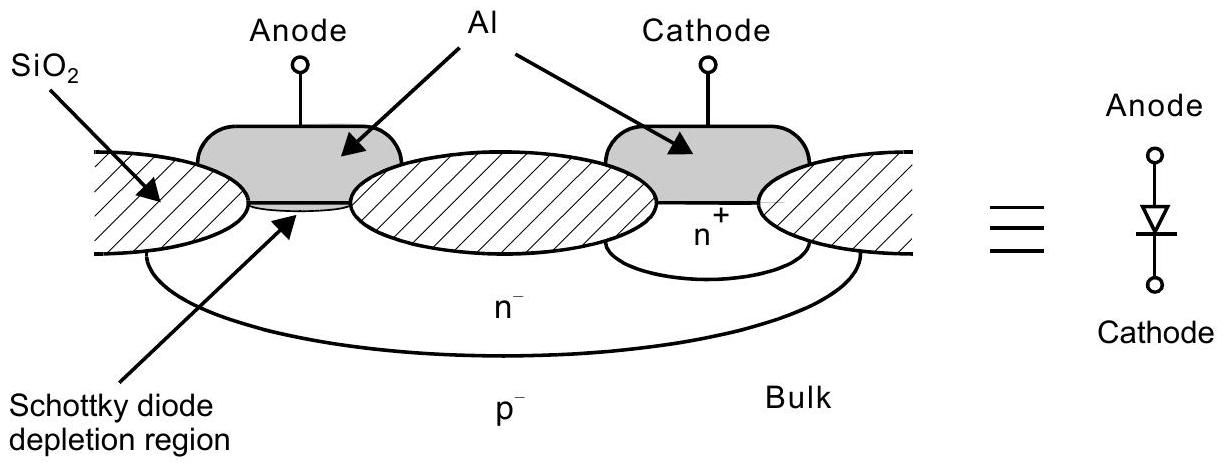
\includegraphics[max width=\textwidth, center]{2024_10_31_60860e27b87166db2267g-037}

Fig. 1.5 A cross section of a Schottky diode.

\subsection*{1.2 MOS TRANSISTORS}
Presently, the most popular technology for realizing microcircuits makes use of MOS transistors. Unlike most bipolar junction transistor (BJT) technologies, which make dominant use of only one type of transistor (npn transistors in the case of BJT processes ${ }^{4}$ ), MOS circuits normally use two complementary types of transistors-n-channel and p -channel. While n -channel devices conduct with a positive gate voltage, p -channel devices conduct with a negative gate voltage. Moreover, electrons are used to conduct current in n -channel transistors, while holes are used in p-channel transistors. Microcircuits containing both n-channel and p-channel transistors are called CMOS circuits, for complementary MOS. The acronym MOS stands for metal-oxide semiconductor, which historically denoted the gate, insulator, and channel region materials, respectively. However, most present CMOS technologies utilize polysilicon gates rather than metal gates.

Before CMOS technology became widely available, most MOS processes made use of only n-channel transistors (NMOS). However, often two different types of $n$-channel transistors could be realized. One type, enhancement n-channel transistors, is similar to the n-channel transistors realized in CMOS technologies. Enhancement transistors require a positive gate-to-source voltage to conduct current. The other type, depletion transistors, conduct current with a gate-source voltage of 0 V . Depletion transistors were used to create highimpedance loads in NMOS logic gates.

Key Point: The source terminal of an $n$-channel transistor is defined as whichever of the two terminals has a lower voltage. For a p-channel transistor, the source would be the terminal with the higher voltage.

A typical cross section of an n-channel enhancement-type MOS transistor is shown in Fig. 1.6. With no voltage applied to the gate, the $\mathrm{n}^{+}$source and drain regions are separated by the $\mathrm{p}^{-}$substrate. The distance between the drain and the source is called the channel length, L . In present MOS technologies, the minimum channel length may be as small as 28 nm . It should be noted that there is no physical difference between the drain and the source. ${ }^{5}$ The source terminal of an n-channel transistor is defined as whichever of the two terminals has a lower voltage. For a p-channel transistor, the source would be the terminal with the higher voltage. When a transistor is turned on, current flows from the drain to the source in an n-channel transistor and from the source to the drain in a p-channel transistor. In both cases, the true carriers travel from the source to drain, but the current directions are different because n -channel carriers (electrons) are negative, whereas p -channel carriers (holes) are positive.\\
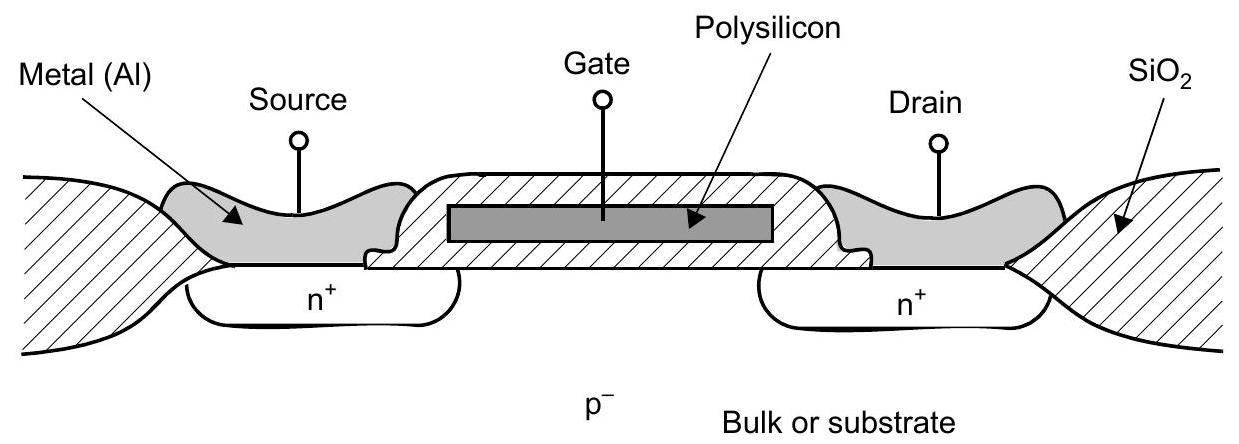
\includegraphics[max width=\textwidth, center]{2024_10_31_60860e27b87166db2267g-038}

Fig. 1.6 A cross section of a typical n-channel transistor.\\
4. Most BJT technologies can also realize low-speed lateral pnp transistors. Normally these would only be used to realize current sources as they have low gains and poor frequency responses. Recently, bipolar technologies utilizing high-speed vertical pnp transistors, as well as high-speed npn transistors, have become available and are growing in popularity. These technologies are called complementary bipolar technologies.\\
5. Large MOS transistors used for power applications are an exception as they might not be realized with symmetric drain and source junctions.

The gate is normally realized using polysilicon, which is heavily doped noncrystalline (or amorphous) silicon. Polysilicon gates are used (instead of metal) because polysilicon has allowed the dimensions of the transistor to be realized much more accurately during the patterning of the transistor. This higher geometric accuracy has resulted in smaller, faster transistors. However, due to the relatively higher resistance of polysilicon, there are continuous efforts to realize metal gates in CMOS fabrication technologies.

The gate is physically separated from the surface of the silicon by a thin insulator made of silicon dioxide $\left(\mathrm{SiO}_{2}\right)$. Thus, the gate is electrically isolated from the channel and affects the channel (and hence, the transistor current) only through electrostatic (capacitive) coupling. The typical thickness of the $\mathrm{SiO}_{2}$ insulator between the gate and the channel is presently between 1 to 30 nm . Since the gate is electrically isolated from the channel, it does not conduct appreciable dc current. However, because of the inherent capacitances in MOS transistors, transient gate currents do exist when gate voltage is quickly changing.

Normally the $\mathrm{p}^{-}$substrate (or bulk) is connected to the most negative voltage in a microcircuit. In analog circuits, this might be the negative power supply, and in digital circuits it is normally ground or 0 V . This connection results in all transistors placed in the substrate being surrounded by reverse-biased junctions, which electrically isolate the transistors and thereby prevent conduction between the transistor terminals and the substrate (unless, of course, they are connected together through some other means).

\subsection*{1.2.1 Symbols for MOS Transistors}
Many symbols have been used to represent MOS transistors. Figure 1.7 shows some of the symbols that have been used to represent n-channel MOS transistors. The symbol in Fig. 1.7(a) is often used; note that there is nothing in the symbol to specify whether the transistor is n -channel or p -channel. A common rule is to assume, when in doubt, that the transistor is an n -channel transistor. The symbol in Fig. 1.7(a) will be used occasionally in this text when there is no need to distinguish between the drain and source terminals. Figure $1.7(b)$ is the most commonly used symbol for an n -channel transistor in analog design and is used most often throughout this text. An arrow points outward on the source terminal to indicate that the transistor is $n$-channel and indicates the direction of current.

MOS transistors are actually four-terminal devices, with the substrate being the fourth terminal. In n -channel devices, the $\mathrm{p}^{-}$substrate is normally connected to the most negative voltage in the microcircuit, whereas for p -channel devices, the $\mathrm{n}^{-}$substrate is normally connected to the most positive voltage. In these cases the substrate connection is normally not shown in the symbol. However, for CMOS technologies, at least one of the two types of transistors will be formed in a well substrate that need not be connected to one of the power supply nodes. For example, an $n$-well process would form $n$-channel transistors in a $\mathrm{p}^{-}$substrate encompassing the entire microcircuit, while the p -channel transistors would be formed in many separate $n$-well substrates. In this case, most of the n-well substrates would be connected to the most positive power supply, while some might be connected to other nodes in the circuit (often the well is connected to the source of a transistor that is not connected to the power supply). In these cases, the symbol shown in Fig. 1.7(c) can be used to show the substrate connection explicitly. Note that the arrow points from the p substrate region to the n -channel region, just like the arrow in the diode symbol which points from the p anode to the n cathode region. It should be noted that this case is not encountered often in digital circuits and is more common in analog circuits. Sometimes, in the interest of simplicity, the isolation of the gate is not explicitly shown, as is the case of the symbol of Fig. 1.7(d). This simple notation is more common for\\
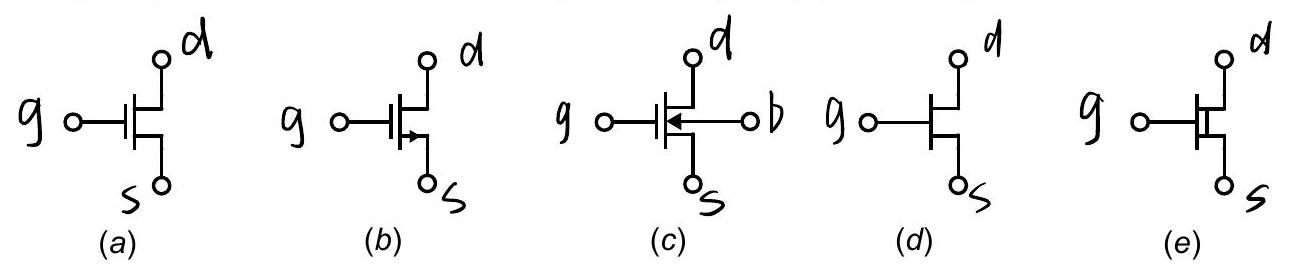
\includegraphics[max width=\textwidth, center]{2024_10_31_60860e27b87166db2267g-039}

Fig. 1.7 Commonly used symbols for n-channel transistors.\\
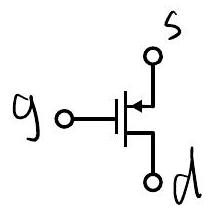
\includegraphics[max width=\textwidth, center]{2024_10_31_60860e27b87166db2267g-040}\\
(a)\\
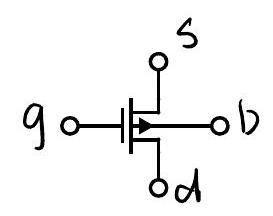
\includegraphics[max width=\textwidth, center]{2024_10_31_60860e27b87166db2267g-040(2)}\\
(b)\\
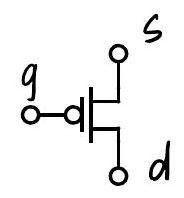
\includegraphics[max width=\textwidth, center]{2024_10_31_60860e27b87166db2267g-040(1)}\\
(c)\\
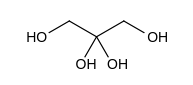
\includegraphics{smile-6c543c520dbe4e1cd3573d4ae35ded594fe700ba}\\
(d)\\
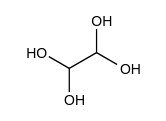
\includegraphics{smile-c5435010ee139e67aa1ff93410cbd05206174048}\\
(e)

Fig. 1.8 Commonly used symbols for p-channel transistors.\\
digital circuits in which a large number of transistors are present. Since this symbol is also used for JFET transistors, it will never be used to represent MOS transistors in this text. The last symbol, shown in Fig. 1.7(e), denotes an n -channel depletion transistor. The extra line is used to indicate that a physical channel exists for a $0-\mathrm{V}$ gatesource voltage. Depletion transistors were used in older NMOS technologies but are not typically available in CMOS processes.

Figure 1.8 shows some commonly used symbols for p-channel transistors. In this text, the symbol of Fig. 1.8(a) will be most often used. The symbol in Fig. 1.8(c) is sometimes used in digital circuits, where the circle indicates that a low voltage on the gate turns the transistor on, as opposed to a high voltage for an n -channel transistor Fig. 1.7(a). The symbols of Fig. 1.8(d) or Fig. 1.8(e) might be used in larger circuits where many transistors are present, to simplify the drawing somewhat. They will not be used in this text.

\subsection*{1.2.2 Basic Operation}
The basic operation of MOS transistors will be described with respect to an n -channel transistor. First, consider the simplified cross sections shown in Fig. 1.9, where the source, drain, and substrate are all connected to ground. In this case, the MOS transistor operation is similar to a capacitor. The gate acts as one plate of the capacitor, and the surface of the silicon, just under the thin insulating $\mathrm{SiO}_{2}$, acts as the other plate.

If the gate voltage is very negative, as shown in Fig. 1.9(a), positive charge will be attracted to the channel region. Since the substrate was originally doped $\mathrm{p}^{-}$, this negative gate voltage has the effect of simply increasing the channel doping to $\mathrm{p}^{+}$, resulting in what is called an accumulated channel. The $\mathrm{n}^{+}$source and drain regions are separated from the $\mathrm{p}^{+}$-channel region by depletion regions, resulting in the equivalent circuit of two back-to-back diodes. Thus, only leakage current will flow even if one of the source or drain voltages becomes large (unless the drain voltage becomes so large as to cause the transistor to break down).

In the case of a positive voltage being applied to the gate, the opposite situation occurs, as shown in Fig. $1.9(b)$. For small positive gate voltages, the positive carriers in the channel under the gate are initially repulsed and the channel changes from a $\mathrm{p}^{-}$doping level to a depletion region. As a more positive gate voltage is applied, the gate attracts negative charge from the source and drain regions, and the channel becomes an n region with mobile electrons connecting the drain and source regions. ${ }^{6}$ In short, a sufficiently large positive gate-source voltage changes the channel beneath the gate to an n region, and the channel is said to be inverted.

The gate-source voltage, for which the concentration of electrons under the gate is equal to the concentration of holes in the $\mathrm{p}^{-}$substrate far from the gate, is commonly referred to as the transistor threshold voltage and denoted $\mathrm{V}_{\mathrm{tn}}$ (for n -channel transistors). For gate-source voltages larger than $\mathrm{V}_{\mathrm{tn}}$, there is an n -type channel present, and conduction between the drain and the source can occur. For gate-source voltages less than $\mathrm{V}_{\mathrm{tn}}$, it is normally assumed that the transistor is off and no current flows between the drain and the source. However, it should be noted that this assumption of zero drain-source current for a transistor that is

\footnotetext{\begin{enumerate}
  \setcounter{enumi}{5}
  \item The drain and source regions are sometimes called diffusion regions or junctions for historical reasons. This use of the word junction
\end{enumerate}
}
is not synonymous with our previous use, in which it designated a pn interface of a diode.\\
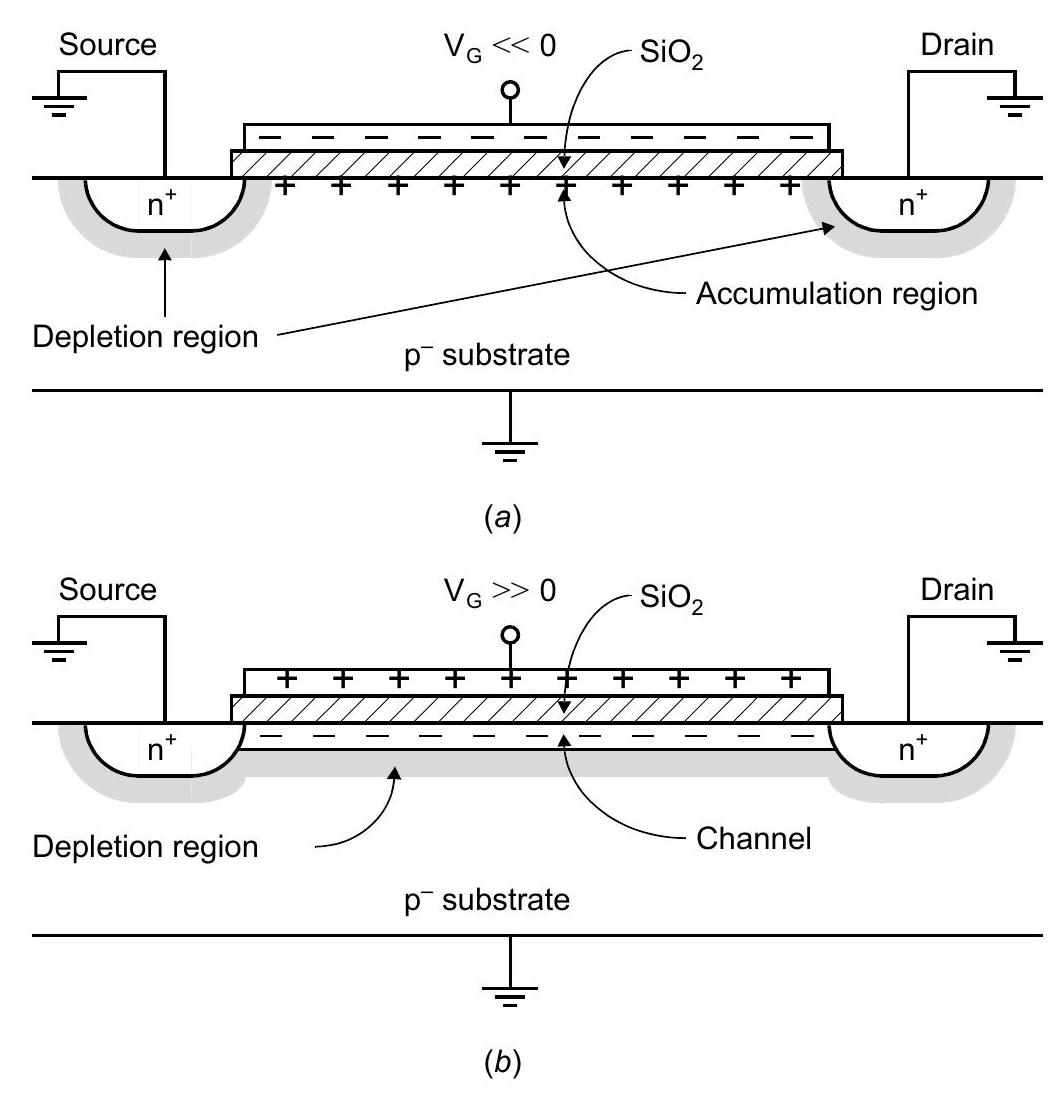
\includegraphics[max width=\textwidth, center]{2024_10_31_60860e27b87166db2267g-041}

Fig. 1.9 An n-channel MOS transistor. (a) $\mathrm{V}_{\mathrm{G}} \ll 0$, resulting in an accumulated channel (no current flow); (b) $\mathrm{V}_{\mathrm{G}}>>0$, and the channel is present (current flow possible from drain to source).\\
off is only an approximation. In fact, for gate voltages around $\mathrm{V}_{\mathrm{tn}}$, there is no abrupt current change, and for gate-source voltages slightly less than $\mathrm{V}_{\mathrm{tn}}$, small amounts of subthreshold current can flow, as discussed in Section 1.4.1.

When the gate-source voltage, $\mathrm{V}_{\mathrm{GS}}$, is larger than $\mathrm{V}_{\mathrm{tn}}$, the channel is present. As $\mathrm{V}_{\mathrm{Gs}}$ is increased, the density of electrons in the channel increases. Indeed, the carrier density, and therefore the charge density, is proportional to $\mathrm{V}_{\mathrm{Gs}}-\mathrm{V}_{\mathrm{t} \mathrm{n}}$, which is often called the effective gate-source voltage and denoted $\mathrm{V}_{\text {eff }}$. Specifically, define


\begin{equation*}
\mathrm{V}_{\mathrm{eff}} \equiv \mathrm{~V}_{\mathrm{GS}}-\mathrm{V}_{\mathrm{tn}} \tag{1.50}
\end{equation*}


The charge density of electrons is then given by


\begin{equation*}
Q_{n}=C_{o x}\left(V_{G S}-V_{\mathrm{tn}}\right)=C_{o x} V_{\text {eff }} \tag{1.51}
\end{equation*}


Here, $C_{0 x}$ is the gate capacitance per unit area and is given by


\begin{equation*}
\mathrm{C}_{\mathrm{ox}}=\frac{\mathrm{K}_{\mathrm{ox}} \varepsilon_{0}}{\mathrm{t}_{\mathrm{ox}}} \tag{1.52}
\end{equation*}


where $\mathrm{K}_{\mathrm{ox}}$ is the relative permittivity of $\mathrm{SiO}_{2}$ (approximately 3.9) and $\mathrm{t}_{\mathrm{ox}}$ is the thickness of the thin oxide under the gate. A point to note here is that (1.51) is only accurate when both the drain and the source voltages are zero.

To obtain the total gate capacitance, (1.52) should be multiplied by the effective gate area, WL, where W is the gate width and L is the effective gate length. These dimensions are shown in Fig. 1.10. Thus the total gate capacitance, $\mathrm{C}_{\mathrm{g}}$, is given by


\begin{equation*}
C_{g}=W L C_{o x} \tag{1.53}
\end{equation*}


and the total charge of the channel, $Q_{T-n}$, is given by


\begin{equation*}
Q_{T-n}=W L C_{o x}\left(V_{G S}-V_{t n}\right)=W L C_{o x} V_{\text {eff }} \tag{1.54}
\end{equation*}


The gate capacitance is one of the major load capacitances that circuits must be capable of driving. Gate capacitances are also important when one is calculating charge injection, which occurs when a MOS transistor is being turned off because the channel charge, $Q_{T-n}$, must flow from under the gate out through the terminals to other places in the circuit.

Next, if the drain voltage is increased above 0 V , a drain-source potential difference exists. This difference results in current flowing from the drain to the source. ${ }^{7}$ The relationship between $\mathrm{V}_{\mathrm{DS}}$ and the drain-source current, $I_{D}$, is the same as for a resistor, assuming $V_{D S}$ is small. This relationship is given [Sze, 1981] by


\begin{equation*}
\mathrm{I}_{\mathrm{D}}=\mu_{\mathrm{n}} \mathrm{Q}_{\mathrm{n}} \frac{\mathrm{~W}}{\mathrm{~L}} \mathrm{~V}_{\mathrm{DS}} \tag{1.55}
\end{equation*}


where $\mu_{n}$ is the mobility of electrons near the silicon surface, and $Q_{n}$ is the charge concentration of the channel per unit area (looking from the top down). Electron mobility is $0.14 \mathrm{~m}^{2} / \mathrm{Vs}$ in pure intrinsic silicon, decreasing with increasing dopant concentrations to $\mu_{n} \cong 0.01-0.06 \mathrm{~m}^{2} / \mathrm{Vs}$ in modern NMOS devices. Note that as the channel length increases, the drain-source current decreases, whereas this current increases as either the charge density or the transistor width increases. Using (1.54) and (1.55) results in


\begin{equation*}
\mathrm{I}_{\mathrm{D}}=\mu_{\mathrm{n}} \mathrm{C}_{\mathrm{ox}} \frac{\mathrm{~W}}{\mathrm{~L}}\left(\mathrm{~V}_{\mathrm{GS}}-\mathrm{V}_{\mathrm{tn}}\right) \mathrm{V}_{\mathrm{DS}}=\mu_{\mathrm{n}} \mathrm{C}_{\mathrm{ox}} \frac{\mathrm{~W}}{\mathrm{~L}} \mathrm{~V}_{\mathrm{eff}} \mathrm{~V}_{\mathrm{DS}} \tag{1.56}
\end{equation*}


where it should be emphasized that this relationship is only valid for drain-source voltages near zero (i.e., $\mathrm{V}_{\mathrm{DS}}$ much smaller than $\mathrm{V}_{\text {eff }}$ ).\\
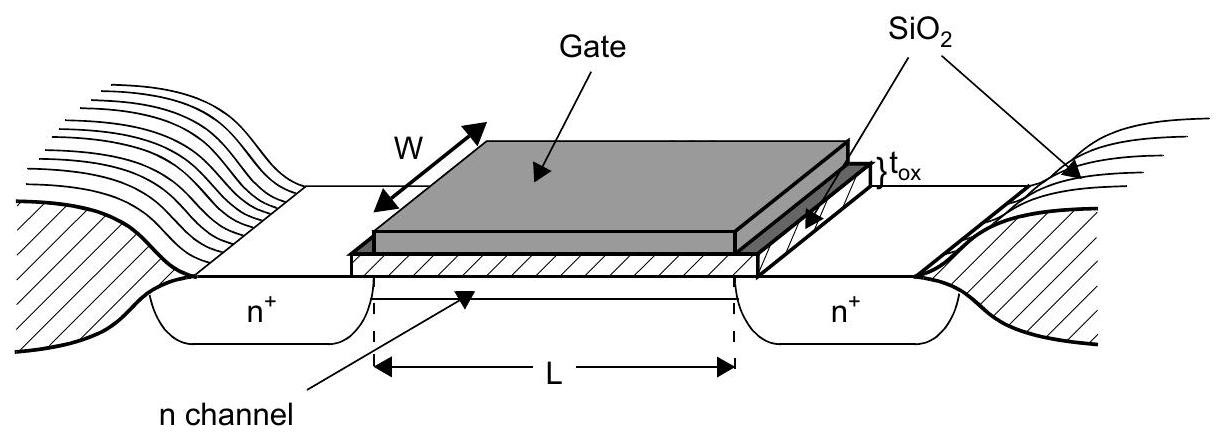
\includegraphics[max width=\textwidth, center]{2024_10_31_60860e27b87166db2267g-042}

Fig. 1.10 The important dimensions of a MOS transistor.

\footnotetext{\begin{enumerate}
  \setcounter{enumi}{6}
  \item The current is actually conducted by negative carriers (electrons) flowing from the source to the drain. Negative carriers flowing
\end{enumerate}
}
from source to drain results in a positive current from drain to source, $\mathrm{I}_{\mathrm{DS}}$.\\
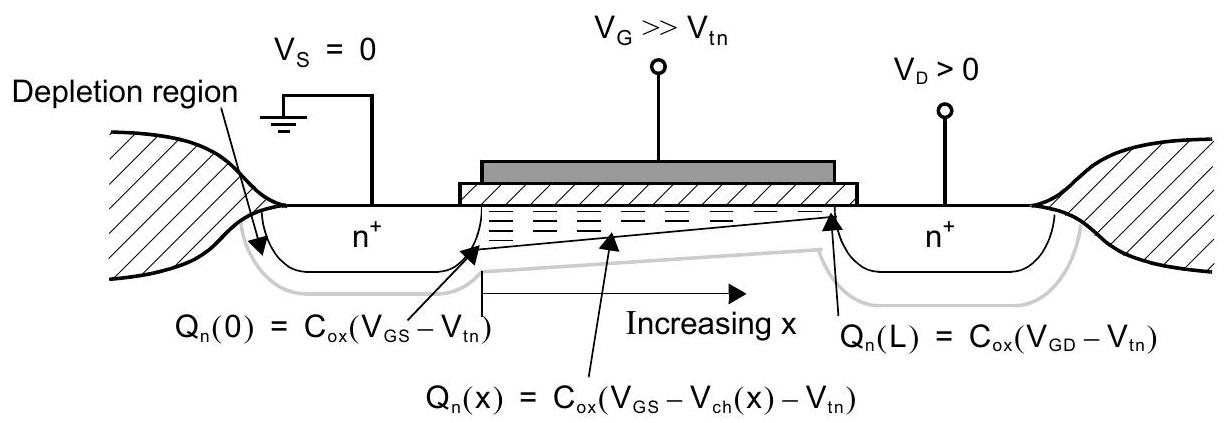
\includegraphics[max width=\textwidth, center]{2024_10_31_60860e27b87166db2267g-043(1)}

Fig. 1.11 The channel charge density for $\mathrm{V}_{\mathrm{DS}}>0$.

As the drain-source voltage increases, the channel charge concentration decreases at the drain end. This decrease is due to the smaller gate-to-channel voltage difference across the thin gate oxide as one moves closer to the drain. In other words, since the drain voltage is assumed to be at a higher voltage than the source, there is an increasing voltage gradient from the source to the drain, resulting in a smaller gate-to-channel voltage near the drain. Since the charge density at a distance $x$ from the source end of the channel is proportional to $\mathrm{V}_{\mathrm{G}}-\mathrm{V}_{\mathrm{ch}}(\mathrm{x})-\mathrm{V}_{\mathrm{tn}}$, as $\mathrm{V}_{\mathrm{G}}-\mathrm{V}_{\mathrm{ch}}(\mathrm{x})$ decreases, the charge density also decreases. ${ }^{8}$ This

Key Point: The relationship between drainsource voltage and drain current of a MOS device is approximately linear when $\mathrm{V}_{\mathrm{DS}} \ll \mathrm{V}_{\text {eff }}$.\\
effect is illustrated in Fig. 1.11.

Note that at the drain end of the channel, we have


\begin{equation*}
V_{G}-V_{c h}(L)=V_{G D} \tag{1.57}
\end{equation*}


For small $V_{D S}$, we saw from (1.56) that $I_{D}$ was linearly related to $\mathrm{V}_{\mathrm{DS}}$. However, as $\mathrm{V}_{\mathrm{DS}}$ increases, and the charge density decreases near the drain, the relationship becomes nonlinear. In fact, the linear relationship for $I_{D}$ versus $V_{D S}$ flattens for larger $\mathrm{V}_{\mathrm{DS}}$, as shown in Fig. 1.12.

As the drain voltage is increased, at some point the gate-tochannel voltage at the drain end will decrease to the threshold value $\mathrm{V}_{\mathrm{tn}}$ - the minimum gate-to-channel voltage needed for n carriers in the channel to exist. Thus, at the drain end, the channel becomes pinched off, as shown in Fig. 1.13. This pinch-off occurs at $\mathrm{V}_{\mathrm{GD}}=\mathrm{V}_{\mathrm{tn}}$, since the channel voltage at the drain end is simply equal to $V_{D}$. Thus, pinch-off occurs for


\begin{equation*}
V_{D G}>-V_{t n} \tag{1.58}
\end{equation*}


Denoting $\mathrm{V}_{\mathrm{DS} \text {-sat }}$ as the drain-source voltage when the channel becomes pinched off, we can substitute $V_{D G}=V_{D S}-V_{G S}$ into\\
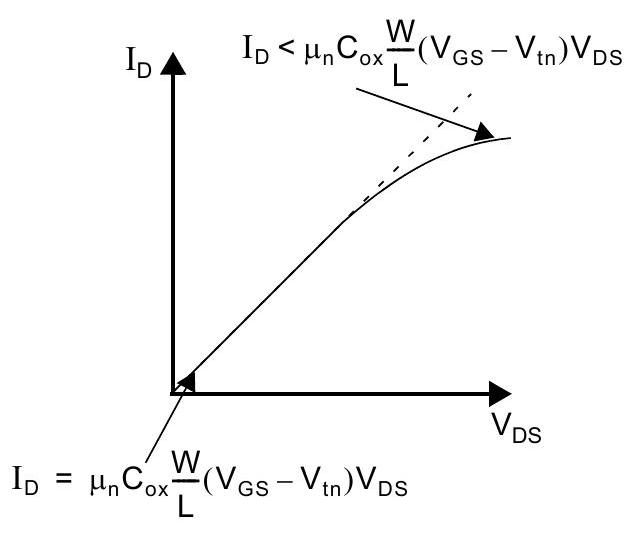
\includegraphics[max width=\textwidth, center]{2024_10_31_60860e27b87166db2267g-043}

Fig. 1.12 For $V_{D S}$ not close to zero, the $I_{D}$ versus $V_{D S}$ relationship is no longer linear.\\
(1.58) and find an equivalent pinch-off expression


\begin{equation*}
V_{D S}>V_{D S-s a t} \tag{1.59}
\end{equation*}


\footnotetext{\begin{enumerate}
  \setcounter{enumi}{7}
  \item $\mathrm{V}_{\mathrm{G}}-\mathrm{V}_{\mathrm{CH}}(\mathrm{x})$ is the gate-to-channel voltage drop at distance x from the source end, with $\mathrm{V}_{\mathrm{G}}$ being the same everywhere in the gate,
\end{enumerate}
}
since the gate material is highly conductive.\\
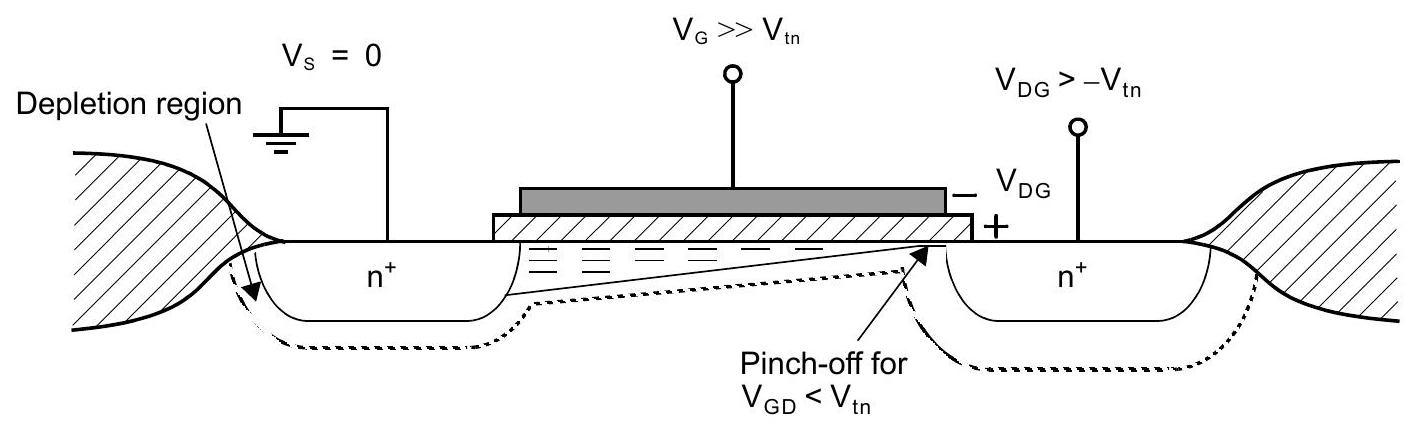
\includegraphics[max width=\textwidth, center]{2024_10_31_60860e27b87166db2267g-044}

Fig. 1.13 When $\mathrm{V}_{\mathrm{DS}}$ is increased so that $\mathrm{V}_{\mathrm{GD}}<\mathrm{V}_{\mathrm{tn}}$, the channel becomes pinched off at the drain end.\\
where $\mathrm{V}_{\mathrm{DS} \text {-sat }}$ is given ${ }^{9}$ by


\begin{equation*}
V_{D S-s a t}=V_{G S}-V_{t n}=V_{\text {eff }} \tag{1.60}
\end{equation*}


The current travelling through the pinched-off channel region is saturated, similar to a gas under pressure travelling through a very small tube. If the drain-gate voltage rises above this critical pinch-off voltage of $-\mathrm{V}_{\mathrm{tn}}$, the charge concentration in the channel remains constant (to a first-order approximation) and the drain current no longer increases with increasing $\mathrm{V}_{\mathrm{DS}}$. The result is the current-voltage relationship shown in Fig. 1.14 for a given gate-source voltage. In the region of operation where $\mathrm{V}_{\mathrm{DS}}>\mathrm{V}_{\mathrm{DS} \text {-sat }}$, the drain current is independent of $\mathrm{V}_{\mathrm{DS}}$ and is called the active region. ${ }^{10}$ The region where $\mathrm{I}_{\mathrm{D}}$ changes linearly with $\mathrm{V}_{\mathrm{DS}}$ is called the triode region. When MOS transistors are used in analog amplifiers, they almost always are biased in the active region. When they are used in digital logic gates, they often operate in both regions.

It is sometimes necessary to distinguish between transistors in weak, moderate, and strong inversion. As just discussed, a gate-source voltage greater than $\mathrm{V}_{\mathrm{tn}}$ results in an inverted channel, and drain-source current can flow. However, as the gate-source voltage is increased, the channel does not become inverted (i.e., n-region) suddenly,

$$
\mathrm{I}_{\mathrm{D}}=\mu_{\mathrm{n}} \mathrm{C}_{\mathrm{ox}} \frac{\mathrm{~W}}{\mathrm{~L}}\left[\left(\mathrm{~V}_{\mathrm{GS}}-\mathrm{V}_{\mathrm{tn}}\right) \mathrm{V}_{\mathrm{DS}}-\frac{\mathrm{V}_{\mathrm{DS}}^{2}}{2}\right] \text { : }
$$

\footnotetext{\begin{enumerate}
  \setcounter{enumi}{8}
  \item Because of the body effect, the threshold voltage at the drain end of the transistor is increased, resulting in the true value of $\mathrm{V}_{\mathrm{DS} \text {-sat }}$ being slightly lower than $\mathrm{V}_{\text {eff }}$.
  \item The active region may also be called the saturation region, but this can lead to confusion because in the case of bipolar transistors, the saturation region occurs for small $\mathrm{V}_{\mathrm{CE}}$, whereas for MOS transistors it occurs for large $\mathrm{V}_{\mathrm{DS}}$. Moreover, we shall see that the drain current does not truly saturate, but continues to increase slightly with increasing drain-source voltage.
\end{enumerate}
}
but rather gradually. Thus, it is useful to define three regions of channel inversion with respect to the gate-source voltage. In most circuit applications, noncutoff MOSFET transistors are operated in strong inversion, with $\mathrm{V}_{\text {eff }}>100 \mathrm{mV}$ (many prudent circuit designers use a minimum value of 200 mV ). As the name suggests, strong inversion occurs when the channel is strongly inverted. It should be noted that all the equation models in this section assume strong inversion operation. Weak inversion occurs when $\mathrm{V}_{\mathrm{GS}}$ is approximately 100 mV or more below $\mathrm{V}_{\mathrm{tn}}$ and is discussed as subthreshold operation in Section 1.4.1. Finally, moderate inversion is the region between weak and strong inversion.

\subsection*{1.2.3 Large-Signal Modelling}
The triode region equation for a MOS transistor relates the drain current to the gate-source and drain-source voltages. It can be shown (see Appendix) that this relationship is given by


\begin{equation*}
\mathrm{I}_{\mathrm{D}}=\mu_{\mathrm{n}} \mathrm{C}_{\mathrm{ox}}\left(\frac{\mathrm{~W}}{\mathrm{~L}}\right)\left[\left(\mathrm{V}_{\mathrm{GS}}-\mathrm{V}_{\mathrm{tn}}\right) \mathrm{V}_{\mathrm{DS}}-\frac{\mathrm{V}_{\mathrm{DS}}^{2}}{2}\right] \tag{1.61}
\end{equation*}


As $V_{D S}$ increases, $I_{D}$ increases until the drain end of the channel becomes pinched off, and then $I_{D}$ no longer increases. This pinch-off occurs for $\mathrm{V}_{\mathrm{DG}}=-\mathrm{V}_{\mathrm{tn}}$, or approximately,


\begin{equation*}
V_{D S}=V_{G S}-V_{t n}=V_{\text {eff }} \tag{1.62}
\end{equation*}


Right at the edge of pinch-off, the drain current resulting from (1.61) and the drain current in the active region (which, to a first-order approximation, is constant with respect to $\mathrm{V}_{\mathrm{DS}}$ ) must have the same value. Therefore, the active region equation can be found by substituting (1.62) into (1.61), resulting in


\begin{equation*}
I_{D}=\frac{\mu_{\mathrm{n}} C_{o x}}{2}\left(\frac{W}{L}\right)\left(V_{G S}-V_{t n}\right)^{2} \tag{1.63}
\end{equation*}


For $\mathrm{V}_{\mathrm{DS}}>\mathrm{V}_{\text {eff }}$, the current stays constant at the value given by (1.63), ignoring second-order effects such as channel-length modulation. This equation is perhaps the most important one that describes the large-signal operation of a MOS transistor. It should be noted here that (1.63) represents a square-law current-voltage relationship for a MOS transistor in the active region. In the case of a BJT transistor, an exponential current-voltage relationship exists in the active region.

Key Point: For $\mathrm{V}_{\mathrm{DS}}>\mathrm{V}_{\mathrm{eff}}$, MOS device exhibits a square-law current-voltage relationship.

As just mentioned, (1.63) implies that the drain current, $I_{D}$, is independent of the drain-source voltage. This independence is only true to a first-order approximation. The major source of error is due to the channel length shrinking as $\mathrm{V}_{\mathrm{DS}}$ increases. To see this effect, consider Fig. 1.15, which shows a cross section of a transistor in the\\
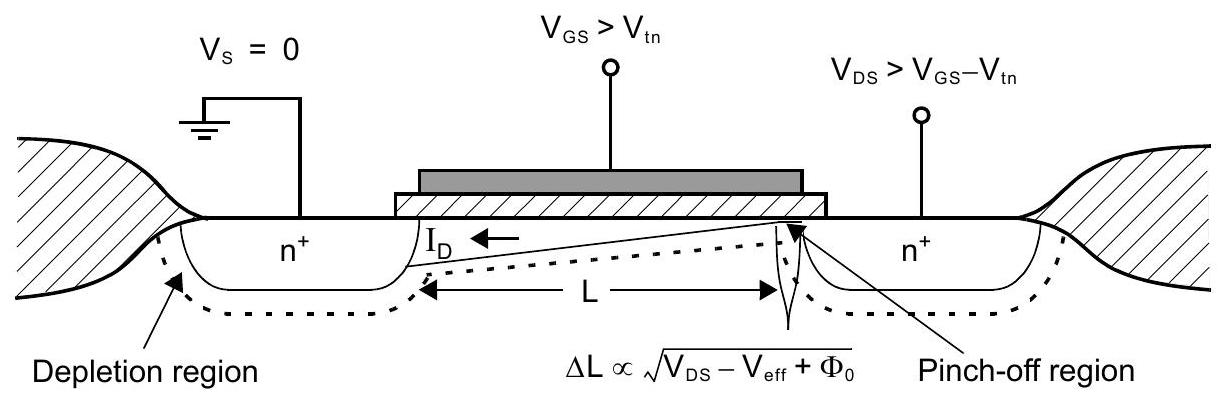
\includegraphics[max width=\textwidth, center]{2024_10_31_60860e27b87166db2267g-045}

Fig. 1.15 Channel length shortening for $\mathrm{V}_{\mathrm{DS}}>\mathrm{V}_{\text {eff }}$.\\
active region. A pinched-off region with very little charge exists between the drain and the channel. The voltage at the end of the channel closest to the drain is fixed at $\mathrm{V}_{\mathrm{Gs}}-\mathrm{V}_{\mathrm{tn}}=\mathrm{V}_{\text {eff }}$. The voltage difference between the drain and the near end of the channel lies across a short depletion region often called the pinch-off region. As $\mathrm{V}_{\mathrm{DS}}$ becomes larger than $\mathrm{V}_{\text {eff }}$, this depletion region surrounding the drain junction increases its width in a square-root relationship with respect to $\mathrm{V}_{\mathrm{DS}}$. This increase in the width of the depletion region surrounding the drain junction decreases the effective channel length. In turn, this decrease in effective channel length increases the drain current, resulting in what is commonly referred to as channel-length modulation.

To derive an equation to account for channel-length modulation, we first make use of (1.11) and denote the width of the depletion region by $\mathrm{x}_{\mathrm{d}}$, resulting in


\begin{align*}
\mathrm{x}_{\mathrm{d}} & \cong \mathrm{k}_{\mathrm{ds}} \sqrt{V_{\mathrm{D}-\mathrm{ch}}+\Phi_{0}}  \tag{1.64}\\
& =\mathrm{k}_{\mathrm{ds}} \sqrt{V_{\mathrm{DG}}+\mathrm{V}_{\mathrm{tn}}+\Phi_{0}}
\end{align*}


where


\begin{equation*}
\mathrm{k}_{\mathrm{ds}}=\sqrt{\frac{2 \mathrm{~K}_{\mathrm{s}} \varepsilon_{0}}{\mathrm{qN}}} \tag{1.65}
\end{equation*}


and has units of $m / \sqrt{V}$. Note that $N_{A}$ is used here since the $n$-type drain region is more heavily doped than the p-type channel (i.e., $N_{D} \gg N_{A}$ ). By writing a Taylor approximation for $I_{D}$ around its operating value of $V_{D S}=V_{G S}-V_{t n}=V_{\text {eff }}$, we find $I_{D}$ to be given by


\begin{equation*}
I_{D}=I_{D-s a t}+\left(\frac{\partial I_{D}}{\partial L}\right)\left(\frac{\partial L}{\partial V_{D S}}\right) \Delta V_{D S} \cong I_{D-s a t}\left(1+\frac{k_{d s}\left(V_{D S}-V_{\text {eff }}\right)}{2 L \sqrt{V_{D G}+V_{t n}+\Phi_{0}}}\right) \tag{1.66}
\end{equation*}


where $I_{D \text {-sat }}$ is the drain current when $V_{D S}=V_{\text {eff }}$, or equivalently, the drain current when the channel-length modulation is ignored. Note that in deriving the final equation of (1.66), we have used the relationship $\partial \mathrm{L} / \partial \mathrm{V}_{\mathrm{DS}}=-\partial \mathrm{x}_{\mathrm{d}} / \partial \mathrm{V}_{\mathrm{DS}}$. Usually, (1.66) is written as


\begin{equation*}
I_{D}=\frac{\mu_{n} C_{o x}}{2}\left(\frac{W}{L}\right)\left(V_{G S}-V_{t n}\right)^{2}\left[1+\lambda\left(V_{D S}-V_{\text {eff }}\right)\right] \tag{1.67}
\end{equation*}


where $\lambda$ is the output impedance constant (in units of $\mathrm{V}^{-1}$ ) given by


\begin{equation*}
\lambda=\frac{k_{\mathrm{ds}}}{2 L \sqrt{V_{D G}+V_{t n}+\Phi_{0}}}=\frac{k_{d s}}{2 L \sqrt{V_{D S}-V_{\text {eff }}+\Phi_{0}}} \tag{1.68}
\end{equation*}


Equation (1.67) is accurate until $\mathrm{V}_{\mathrm{DS}}$ is large enough to cause second-order effects, often called short-channel effects. For example, (1.67) assumes that current flow down the channel is not velocity-saturated, in which case increasing the electric field no longer increases the carrier speed. Short-channel effects cause $I_{D}$ to deviate from the result predicted by (1.67) and are discussed in Section 1.4. Of course, for quite large values of $\mathrm{V}_{\mathrm{DS}}$, the transistor will eventually break down.

A plot of $I_{D}$ versus $V_{D S}$ for different values of $V_{G S}$ is shown in Fig. 1.16. Note that in the active region, the small (but nonzero) slope indicates the small dependence of $I_{D}$ on $V_{D S}$.\\
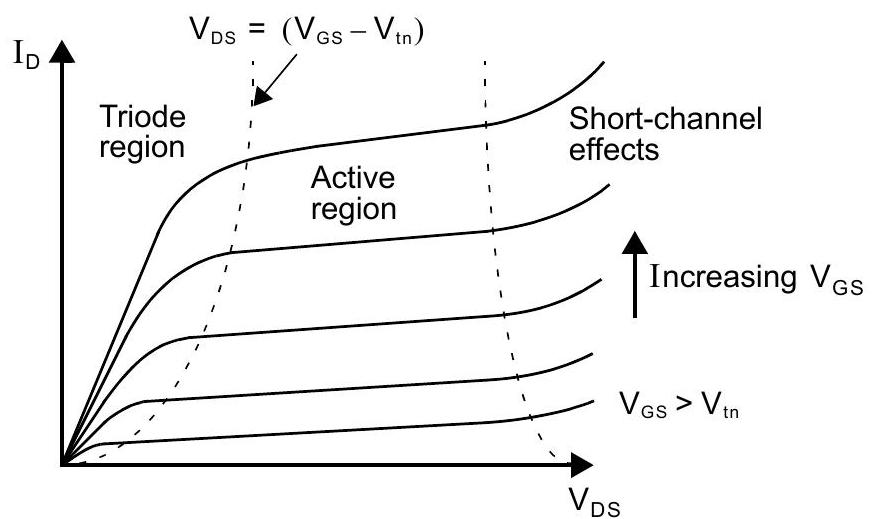
\includegraphics[max width=\textwidth, center]{2024_10_31_60860e27b87166db2267g-047}

Fig. 1.16 $\quad I_{D}$ versus $V_{D S}$ for different values of $V_{G S}$.

\section*{EXAMPLE 1.8}
Find $I_{D}$ for an $n$-channel transistor that has doping concentrations of $N_{D}=10^{25}$ electrons $/ \mathrm{m}^{3}$, $\mathrm{N}_{\mathrm{A}}=5 \times 10^{22}$ holes $/ \mathrm{m}^{3}, \mu_{\mathrm{n}} \mathrm{C}_{\mathrm{ox}}=270 \mu \mathrm{~A} / \mathrm{V}^{2}, \mathrm{~W} / \mathrm{L}=5 \mu \mathrm{~m} / 0.5 \mu \mathrm{~m}, \mathrm{~V}_{\mathrm{GS}}=0.8 \mathrm{~V}, \mathrm{~V}_{\mathrm{tn}}=0.45 \mathrm{~V}$, and $V_{D S}=V_{\text {eff }}$. Assuming $\lambda$ remains constant, estimate the new value of $I_{D}$ if $V_{D S}$ is increased by 0.5 V .

\section*{Solution}
From (1.65), we have

$$
\mathrm{k}_{\mathrm{ds}}=\sqrt{\frac{2 \times 11.8 \times 8.854 \times 10^{-12}}{1.6 \times 10^{-19} \times 5 \times 10^{22}}}=162 \times 10^{-9} \mathrm{~m} / \sqrt{\mathrm{V}}
$$

which is used in (1.68) to find $\lambda$ as

$$
\lambda=\frac{162 \times 10^{-9}}{2 \times 0.5 \times 10^{-6} \times \sqrt{0.9}}=0.171 \mathrm{~V}^{-1}
$$

Using (1.67), we find for $\mathrm{V}_{\mathrm{DS}}=\mathrm{V}_{\text {eff }}=0.4 \mathrm{~V}$,

$$
I_{D 1}=\left(\frac{270 \times 10^{-6}}{2}\right)\left(\frac{5}{0.5}\right)(0.35)^{2}(1)=165 \mu \mathrm{~A}
$$

In the case where $\mathrm{V}_{\mathrm{Ds}}=\mathrm{V}_{\text {eff }}+0.5 \mathrm{~V}=0.9 \mathrm{~V}$, we have

$$
\mathrm{I}_{\mathrm{D} 2}=165 \mu \mathrm{~A} \times(1+\lambda \times 0.5)=180 \mu \mathrm{~A}
$$

Note that this example shows almost a 10 percent increase in drain current for a 0.5 V increase in drain-source voltage.

\subsection*{1.2.4 Body Effect}
Key Point: The body effect is the influence of the body potential on the channel, modelled as an increase in the threshold voltage, $V_{t n}$, with increasing source-tobody reverse-bias.

The large-signal equations in the preceding section were based on the assumption that the source voltage was the same as the body voltage (i.e., the substrate or bulk voltage or an NMOS device). However, often the source and body can be at different voltages. Looking at Fig. 1.11, it is evident that the body is capacitively coupled to the channel region just as the gate is, albeit through the junction capacitance between them instead of the gate-oxide capacitance. ${ }^{11}$ Hence, the amount of charge in the channel and conduction through it is influenced by the potential difference between body and source.

Typically called the body effect, the influence of the body potential on the channel is modelled as an increase in the threshold voltage, $\mathrm{V}_{\mathrm{tn}}$, with increasing source-to-body reverse-bias voltage. The body effect is more important for transistors in a well of a CMOS process where the body terminal's doping concentration is higher and the resulting junction capacitance between body and channel is larger. The body effect is often important in analog circuit designs and should not be ignored.

To account for the body effect, it can be shown (see Appendix at the end of this chapter) that the threshold voltage of an n -channel transistor is now given by


\begin{equation*}
\mathrm{V}_{\mathrm{tn}}=\mathrm{V}_{\mathrm{tn} 0}+\gamma\left(\sqrt{\mathrm{V}_{\mathrm{SB}}+\left|2 \phi_{\mathrm{F}}\right|}-\sqrt{\left|2 \phi_{\mathrm{F}}\right|}\right) \tag{1.69}
\end{equation*}


where $V_{t n 0}$ is the threshold voltage with zero $V_{S B}$ (source-to-body voltage), $\phi_{F}=(k T / q) \ln \left(N_{A} / n_{i}\right)$ is the Fermi potential of the body, and


\begin{equation*}
\gamma=\frac{\sqrt{2 \mathrm{qN}_{\mathrm{A}} \mathrm{~K}_{\mathrm{s}} \varepsilon_{0}}}{\mathrm{C}_{\mathrm{ox}}} \tag{1.70}
\end{equation*}


The factor $\gamma$ is often called the body-effect constant and has units of $\sqrt{\mathrm{V}}$. Notice that $\gamma$ is proportional to $\sqrt{\mathrm{N}_{\mathrm{A}}},{ }^{12}$ so the body effect is larger for transistors in a well where typically the doping is higher than the substrate of the microcircuit.

\subsection*{1.2.5 p-Channel Transistors}
All of the preceding equations have been presented for n -channel enhancement transistors. In the case of p-channel transistors, these equations can also be used if a neg ative sign is placed in front of eve ry voltage variable. Thus, $\mathrm{V}_{\mathrm{GS}}$ becomes $\mathrm{V}_{\mathrm{SG}}, \mathrm{V}_{\mathrm{Ds}}$ becomes $\mathrm{V}_{\mathrm{SD}}, \mathrm{V}_{\mathrm{tn}}$ becomes $-\mathrm{V}_{\mathrm{tp}}$, and so on. The condition required for conduction is now $V_{S G}>V_{t p}$, where $V_{t p}$ is now a negative quantity for an enhancement $p$-channel transistor. ${ }^{13}$ The requirement on the source-drain voltage for a $p$-channel transistor to be in the active region is $\mathrm{V}_{\mathrm{SD}}>\mathrm{V}_{\mathrm{SG}}+\mathrm{V}_{\mathrm{tp}}$. The equations for $\mathrm{I}_{\mathrm{D}}$, in both regions, remain unchanged, because all voltage variables are squared, resulting in positive hole current flow from the source to the drain in p-channel transistors.

\footnotetext{\begin{enumerate}
  \setcounter{enumi}{10}
  \item In fact, JFETs intentionally modulate the conducting channel via a junction capacitance, hence their name: Junction Field-Effect Transistors.
  \item For an $n$-channel transistor. For a $p$-channel transistor, $\gamma$ is proportional to the square root of $N_{D}$.
  \item It is possible to realize depletion p-channel transistors, but these are of little value and seldom worth the extra processing involved. Depletion n -channel transistors are also seldom encountered in CMOS microcircuits, although they might be worth the extra processing involved in some applications, especially if they were in a well.
\end{enumerate}
}\subsection*{1.2.6 Low-Frequency Small-Signal Modelling in the Active Region}
The most commonly used low-frequency small-signal model for a MOS transistor operating in the active region shown in Fig. 1.17. The voltage-controlled current source, $\mathrm{g}_{\mathrm{m}} \mathrm{v}_{\mathrm{gs}}$, is the most important component of the model, with the transistor transconductance $\mathrm{g}_{\mathrm{m}}$ defined as


\begin{equation*}
\mathrm{g}_{\mathrm{m}}=\frac{\partial \mathrm{I}_{\mathrm{D}}}{\partial \mathrm{~V}_{\mathrm{GS}}} \tag{1.71}
\end{equation*}


In the active region, we use (1.63), which is repeated here for convenience,


\begin{equation*}
I_{D}=\frac{1}{2} \mu_{n} C_{o x}\left(\frac{W}{L}\right)\left(V_{G S}-V_{t n}\right)^{2}=\frac{1}{2} \mu_{n} C_{o x}\left(\frac{W}{L}\right) V_{\text {eff }}^{2} \tag{1.72}
\end{equation*}


and we apply the derivative shown in (1.71) to obtain


\begin{equation*}
g_{m}=\frac{\partial I_{D}}{\partial V_{G S}}=\mu_{n} C_{o x} \frac{W}{L}\left(V_{G S}-V_{t n}\right)=\mu_{n} C_{o x} \frac{W}{L} V_{\text {eff }} \tag{1.73}
\end{equation*}


or equivalently,


\begin{equation*}
g_{m}=\mu_{n} C_{o x} \frac{W}{L} V_{\text {eff }} \tag{1.74}
\end{equation*}


where the effective gate-source voltage, $\mathrm{V}_{\text {eff }}$, is defined as $\mathrm{V}_{\text {eff }} \equiv \mathrm{V}_{\mathrm{GS}}-\mathrm{V}_{\mathrm{tn}}$. Thus, we see that the transconductance of a MOS transistor is directly proportional to $\mathrm{V}_{\text {eff }}$.

Sometimes it is desirable to express $g_{m}$ in terms of $I_{D}$ rather than $V_{G s}$. From (1.72), we have


\begin{equation*}
\mathrm{V}_{\mathrm{Gs}}=\mathrm{V}_{\mathrm{tn}}+\sqrt{\frac{2 \mathrm{I}_{\mathrm{D}}}{\mu_{\mathrm{n}} \mathrm{C}_{\mathrm{ox}}(\mathrm{~W} / \mathrm{L})}} \tag{1.75}
\end{equation*}


The second term in (1.75) is the effective gate-source voltage, $\mathrm{V}_{\text {eff }}$, where


\begin{equation*}
V_{\text {eff }}=V_{G S}-V_{t n}=\sqrt{\frac{2 I_{D}}{\mu_{n} C_{o x}(W / L)}} \tag{1.76}
\end{equation*}


Substituting (1.76) in (1.74) results in an alternative expression for $\mathrm{g}_{\mathrm{m}}$.\\
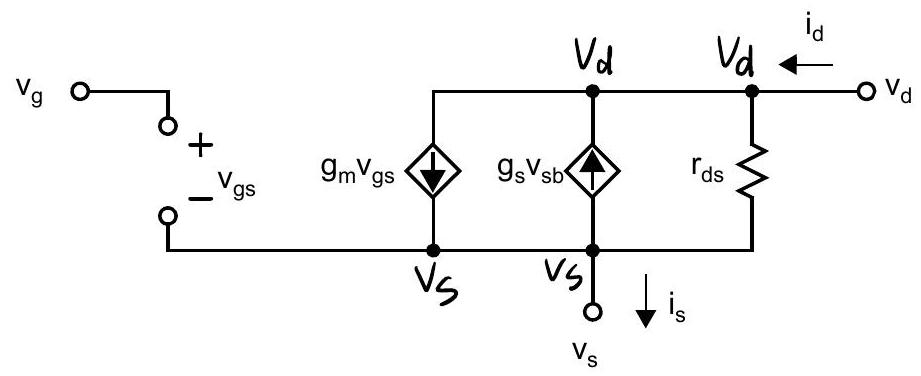
\includegraphics[max width=\textwidth, center]{2024_10_31_60860e27b87166db2267g-049}

Fig. 1.17 The low-frequency, small-signal model for an active MOS transistor.


\begin{equation*}
g_{m}=\sqrt{2 \mu_{n} C_{o x} \frac{W}{L} I_{D}} \tag{1.77}
\end{equation*}


Thus, the transistor transconductance is proportional to $\sqrt{\mathrm{I}_{\mathrm{D}}}$ for a MOS transistor. ${ }^{14}$\\
A third expression for $\mathrm{g}_{\mathrm{m}}$ is found by rearranging (1.77) and then using (1.76) to obtain


\begin{equation*}
g_{m}=\frac{2 I_{D}}{V_{\text {eff }}} \tag{1.78}
\end{equation*}


Key Point: The square-root relationship for transconductance $g_{m}=\sqrt{2 \mu_{\mathrm{n}} C_{0 x}(W / L) I_{D}}$ is useful for circuit analysis when device sizes are fixed. However, the simpler expression $\mathrm{g}_{\mathrm{m}}=2 \mathrm{I}_{\mathrm{D}} / \mathrm{V}_{\text {eff }}$ is useful during initial circuit design when transistor sizes are yet to be determined.

Note that this expression is independent of $\mu_{\mathrm{n}} \mathrm{C}_{\mathrm{ox}}$ and $\mathrm{W} / \mathrm{L}$, and it relates the transconductance to the ratio of drain current to effective gate-source voltage. However, it can cause some confusion for new analog designers as it appears to indicate that transconductance is proportional to drain current, whereas (1.77) indicates a square-root relationship. This discrepancy is resolved by recognizing that increasing $\mathrm{I}_{\mathrm{D}}$ while keeping $\mathrm{V}_{\text {eff }}$ constant implies a proportional increase in (W/L). Hence, (1.77) is useful for analysis where the transistor sizes are given whereas the simple expression in (1.78) can be quite useful during an initial circuit design when the transistor sizes are yet to be determined.

Design often begins with a set of transistor voltage-current measurements, obtained either by experiment or simulation, from which the designer may estimate the device constants $\mu_{n} C_{o x}, V_{t n}$, etc. based on the relationships presented above.

\section*{EXAMPLE 1.9}
The drain current for a particular NMOS device with an aspect ratio $\mathrm{W} / \mathrm{L}=10$ is plotted in Fig. 1.18(a) versus $V_{G S}$ for constant drain, source, and body voltages. From this data, estimate $\mu_{n} C_{o x}$ and $V_{t n}$.

\section*{Solution}
Taking the derivative of Fig. 1.18(a) gives the plot of $\mathrm{g}_{\mathrm{m}}=\delta \mathrm{I}_{\mathrm{D}} / \delta \mathrm{V}_{\mathrm{Gs}}$ in Fig. 1.18(b). Based on the square-law equation (1.74), this plot should be linear in the active region intersecting the line $g_{m}=0$ at $V_{\text {eff }}=0$. Hence, extrapolating the linear portion of the curve in Fig. 1.18(b) provides an intersection at $\mathrm{V}_{\mathrm{Gs}}=\mathrm{V}_{\mathrm{tn}}$. In this case, $\mathrm{V}_{\mathrm{tn}} \cong 450 \mathrm{mV}$. Furthermore, (1.73) shows that the slope of the $\mathrm{g}_{\mathrm{m}}$ versus $\mathrm{V}_{\mathrm{GS}}$ curve should be $\mu_{\mathrm{n}} \mathrm{C}_{\mathrm{ox}}(\mathrm{W} / \mathrm{L})$ in active operation. In Fig. 1.18(b) this slope is approximately $2.7 \mathrm{~mA} / \mathrm{V}^{2}$ which translates to a value of $\mu_{\mathrm{n}} \mathrm{C}_{\mathrm{ox}}=270 \mu \mathrm{~A} / \mathrm{V}^{2}$. These are approximate values, particularly since (1.74) is derived without considering channel-length modulation. However, these values are very useful during design for quickly and roughly estimating the device sizes, currents and voltages required to obtain a desired $\mathrm{g}_{\mathrm{m}}$.

The second voltage-controlled current-source in Fig. 1.17, shown as $\mathrm{g}_{\mathrm{s}} \mathrm{v}_{\mathrm{s}}$, models the body effect on the small-signal drain current, $i_{d}$. When the source is connected to small-signal ground, or when its voltage does not change appreciably, then this current source can be ignored. When the body effect cannot be ignored, we have


\begin{equation*}
\mathrm{g}_{\mathrm{s}}=\frac{\partial \mathrm{I}_{\mathrm{D}}}{\partial \mathrm{~V}_{\mathrm{SB}}}=\frac{\partial \mathrm{I}_{\mathrm{D}}}{\partial \mathrm{~V}_{\mathrm{tn}}} \frac{\partial \mathrm{~V}_{\mathrm{tn}}}{\partial \mathrm{~V}_{\mathrm{SB}}} \tag{1.79}
\end{equation*}


\footnotetext{\begin{enumerate}
  \setcounter{enumi}{13}
  \item Whereas it is proportional to $\mathrm{I}_{\mathrm{C}}$ for a BJT.
\end{enumerate}
}
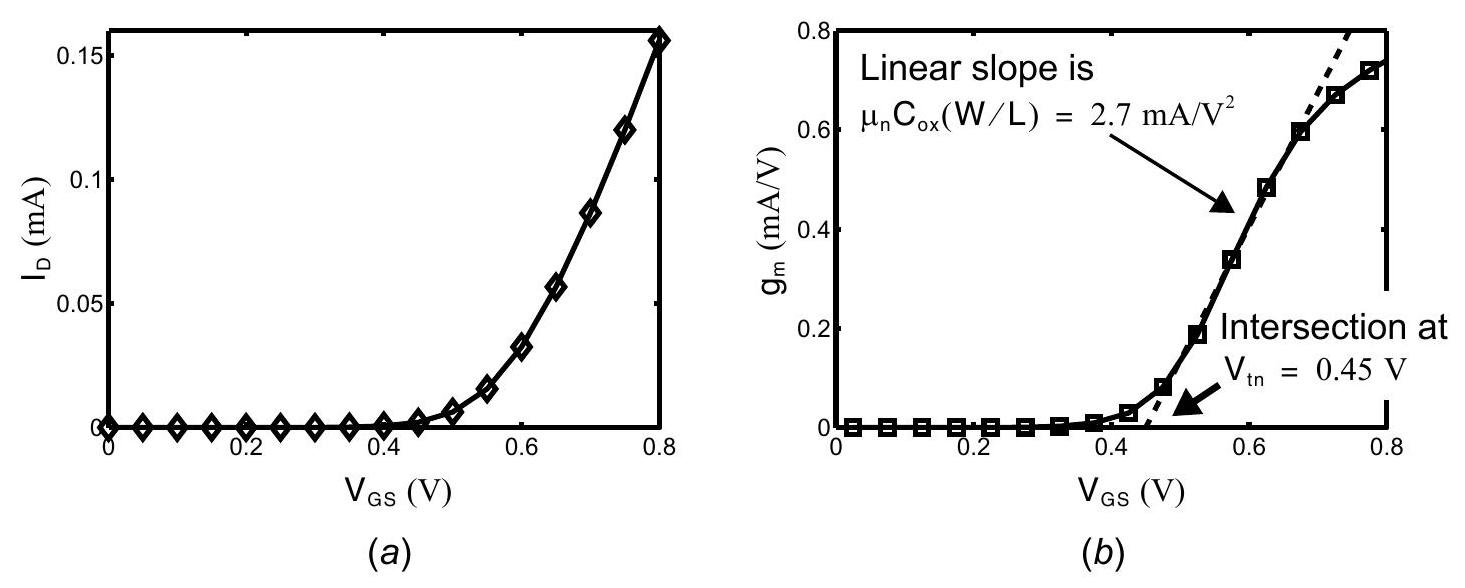
\includegraphics[max width=\textwidth, center]{2024_10_31_60860e27b87166db2267g-051}

Fig. 1.18 Estimation of $\mathrm{V}_{\mathrm{tn}}$ and $\mu_{\mathrm{n}} \mathrm{C}_{\mathrm{ox}}$ from transistor voltage-current data.\\
From (1.72) we have


\begin{equation*}
\frac{\partial \mathrm{I}_{\mathrm{D}}}{\partial \mathrm{~V}_{\mathrm{tn}}}=-\mu_{\mathrm{n}} \mathrm{C}_{\mathrm{ox}}\left(\frac{\mathrm{~W}}{\mathrm{~L}}\right)\left(\mathrm{V}_{\mathrm{GS}}-\mathrm{V}_{\mathrm{tn}}\right)=-\mathrm{g}_{\mathrm{m}} \tag{1.80}
\end{equation*}


Using (1.69), which gives $\mathrm{V}_{\mathrm{tn}}$ as


\begin{equation*}
\mathrm{V}_{\mathrm{tn}}=\mathrm{V}_{\mathrm{tn} 0}+\gamma\left(\sqrt{\mathrm{V}_{\mathrm{SB}}+\left|2 \phi_{\mathrm{F}}\right|}-\sqrt{\left|2 \phi_{\mathrm{F}}\right|}\right) \tag{1.81}
\end{equation*}


we have


\begin{equation*}
\frac{\partial V_{\mathrm{tn}}}{\partial \mathrm{~V}_{\mathrm{SB}}}=\frac{\gamma}{2 \sqrt{\mathrm{~V}_{\mathrm{SB}}+\left|2 \phi_{\mathrm{F}}\right|}} \tag{1.82}
\end{equation*}


The negative sign of (1.80) is eliminated by subtracting the current $\mathrm{g}_{\mathrm{s}} \mathrm{v}_{\mathrm{s}}$ from the major component of the drain current, $\mathrm{g}_{\mathrm{m}} \mathrm{V}_{\mathrm{gs}}$, as shown in Fig. 1.17. Thus, using (1.80) and (1.82), we have


\begin{equation*}
g_{s}=\frac{\gamma g_{m}}{2 \sqrt{V_{S B}+\left|2 \phi_{F}\right|}} \tag{1.83}
\end{equation*}


Note that although $g_{s}$ is nonzero for $V_{S B}=0$, if the source is connected to the bulk $v_{s b}$ is zero and $g_{s}$ may be excluded from the model. However, if the source happens to be biased at the same potential as the bulk but is not directly connected to $i t$, then the effect of $g_{s}$ should be taken into account since there may be nonzero small signals, $\mathrm{V}_{\mathrm{sb}}$.

The resistor, $r_{d s}$, shown in Fig. 1.17, accounts for the finite output impedance (i.e., it models the channellength modulation and its effect on the drain current due to changes in $\mathrm{V}_{\mathrm{DS}}$ ). Using (1.67), repeated here for convenience,


\begin{equation*}
I_{D}=\frac{\mu_{n} C_{o x}}{2}\left(\frac{W}{L}\right)\left(V_{G S}-V_{t n}\right)^{2}\left[1+\lambda\left(V_{D S}-V_{\text {eff }}\right)\right] \tag{1.84}
\end{equation*}


we have


\begin{equation*}
\frac{1}{r_{d s}}=g_{d s}=\frac{\partial I_{D}}{\partial V_{D S}}=\lambda\left(\frac{\mu_{n} C_{o x}}{2}\right)\left(\frac{W}{L}\right)\left(V_{G S}-V_{t n}\right)^{2}=\lambda I_{D-s a t} \cong \lambda I_{D} \tag{1.85}
\end{equation*}


where the approximation assumes $\lambda$ is small, such that we can approximate the drain bias current as being the same as $I_{D-\text { sat }}$. Thus,


\begin{equation*}
r_{\mathrm{ds}} \cong \frac{1}{\lambda \mathrm{I}_{\mathrm{D}}} \tag{1.86}
\end{equation*}


where


\begin{equation*}
\lambda=\frac{\mathrm{k}_{\mathrm{ds}}}{2 \mathrm{~L} \sqrt{\mathrm{~V}_{\mathrm{Ds}}-\mathrm{V}_{\mathrm{eff}}+\Phi_{0}}} \tag{1.87}
\end{equation*}


and


\begin{equation*}
\mathrm{k}_{\mathrm{ds}}=\sqrt{\frac{2 \mathrm{~K}_{\mathrm{s}} \varepsilon_{0}}{\mathrm{qN}}} \tag{1.88}
\end{equation*}


Key Point: Small signalr ds is proportional to $\mathrm{L} / \mathrm{I}_{\mathrm{D}}$.

Substituting (1.87) into (1.86) reveals that $r_{\mathrm{ds}}$ is proportional to $\mathrm{L} / \mathrm{I}_{\mathrm{D}}$. It should be noted here that (1.86) is often empirically adjusted to take into account secondorder effects.

\section*{EXAMPLE 1.10}
Derive the low-frequency model parameters for an n -channel transistor that has doping concentrations of $\mathrm{N}_{\mathrm{D}}=10^{25}$ electrons $/ \mathrm{m}^{3}, \mathrm{~N}_{\mathrm{A}}=5 \times 10^{22}$ holes $/ \mathrm{m}^{3}, \mu_{\mathrm{n}} \mathrm{C}_{\mathrm{ox}}=270 \mu \mathrm{~A} / \mathrm{V}^{2}, \mathrm{~W} / \mathrm{L}=5 \mu \mathrm{~m} / 0.5 \mu \mathrm{~m}, \mathrm{~V}_{\mathrm{GS}}=0.8 \mathrm{~V}$, $\mathrm{V}_{\mathrm{tn}}=0.45 \mathrm{~V}$, and $\mathrm{V}_{\mathrm{DS}}=\mathrm{V}_{\text {eff }}$. Assume $\gamma=0.25 \sqrt{\mathrm{~V}}$ and $\mathrm{V}_{\mathrm{SB}}=0.5 \mathrm{~V}$. What is the new value of $\mathrm{r}_{\mathrm{ds}}$ if the drain-source voltage is increased by 0.5 V ?

\section*{Solution}
Since these parameters are the same as in Example 1.8, we have

$$
\mathrm{g}_{\mathrm{m}}=\frac{2 \mathrm{I}_{\mathrm{D}}}{\mathrm{~V}_{\mathrm{eff}}}=\frac{2 \times 165 \mu \mathrm{~A}}{0.35 \mathrm{~V}}=0.94 \mathrm{~mA} / \mathrm{V}
$$

The Fermi potential of the body at room temperature with $\mathrm{N}_{\mathrm{A}}=5 \times 10^{22}$ holes $/ \mathrm{m}^{3}$ is $\phi_{F}=(\mathrm{kT} / \mathrm{q})$ $\ln \left(N_{A} / n_{i}\right) \cong 0.38 \mathrm{~V}$, and from (1.83) we have

$$
\mathrm{g}_{\mathrm{s}}=\frac{0.25 \times 0.94 \times 10^{-3}}{2 \sqrt{0.5+0.766}}=0.104 \mathrm{~mA} / \mathrm{V}
$$

Note that this source-bulk transconductance value is about 1/9th that of the gate-source transconductance. For $r_{d s}$, we use (1.86) to find

$$
\mathrm{r}_{\mathrm{ds}}=\frac{1}{0.171 \times 165 \times 10^{-6}}=35 \mathrm{k} \Omega
$$

Recalling that $\mathrm{V}_{\text {eff }}=0.35 \mathrm{~V}$, if $\mathrm{V}_{\mathrm{Ds}}$ is increased to 0.85 V , the new value for $\lambda$ is

$$
\lambda=\frac{162 \times 10^{-9}}{2\left(0.5 \times 10^{-6}\right) \sqrt{1.4}}=0.137 \mathrm{~V}^{-1}
$$

resulting in a new value of $r_{d s}$ given by

$$
r_{\mathrm{ds}}=\frac{1}{\lambda \mathrm{I}_{\mathrm{D} 2}}=\frac{1}{0.137 \times 180 \times 10^{-6}} \cong 41 \mathrm{k} \Omega
$$

\section*{EXAMPLE 1.11}
Plotted in Fig. 1.19(a) is the drain current of a particular NMOS device versus its $\mathrm{V}_{\mathrm{DS}}$ with constant gate, source, and body voltages. From this data, estimate the device parameter $\lambda$.

\section*{Solution}
First, rearrange (1.85) into

$$
\lambda=\frac{g_{\mathrm{ds}}}{I_{D-\text { sat }}}=\left(\frac{\partial I_{D}}{\partial V_{D S}}\right) \frac{1}{I_{D-\text { sat }}}
$$

Hence, a plot of $\mathrm{g}_{\mathrm{ds}} / \mathrm{I}_{\mathrm{D}}=\left(\partial \mathrm{I}_{\mathrm{D}} / \partial \mathrm{V}_{\mathrm{DS}}\right) / \mathrm{I}_{\mathrm{D}}$ versus $\mathrm{V}_{\mathrm{DS}}$ for a constant value of $\mathrm{V}_{\mathrm{GS}}$ will be roughly flat in strong inversion providing a rough estimate of $\lambda$. This is done for the present example in Fig. 1.19(b) yielding a value of $\lambda=0.45 \mathrm{~V}^{-1}$. Estimates obtained in this way are only approximate since $r_{d s}$ is subject to many higher-order effects, especially at short channel lengths where $\lambda$ may change by $50 \%$ or even more.\\
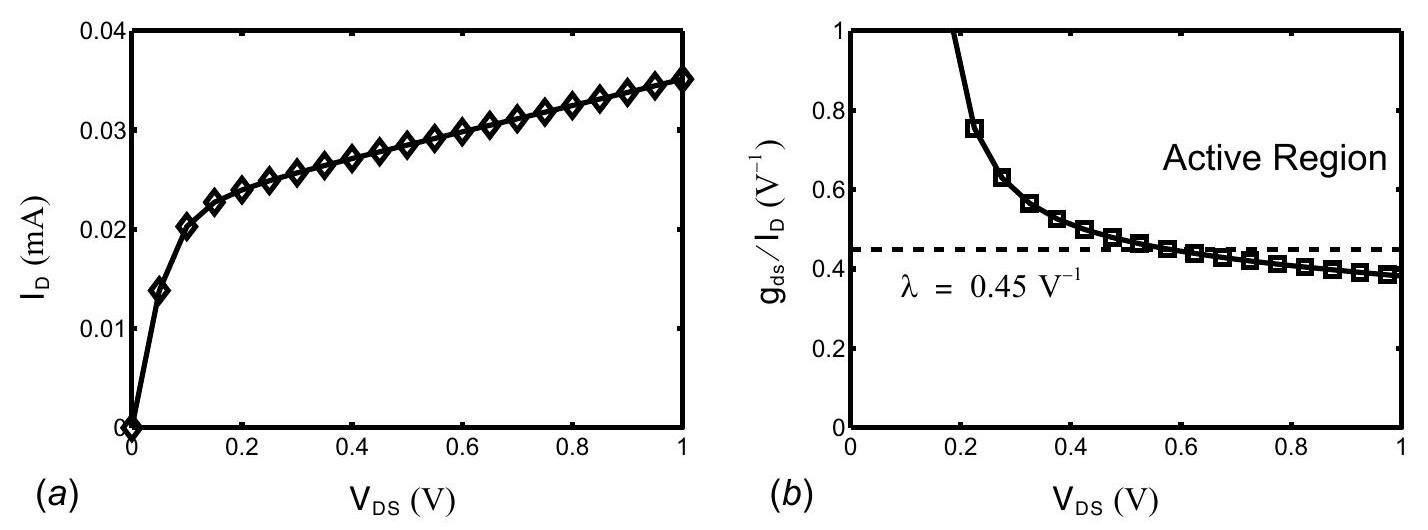
\includegraphics[max width=\textwidth, center]{2024_10_31_60860e27b87166db2267g-053}

Fig. 1.19 Estimation of $\lambda$ from transistor voltage-current data.\\
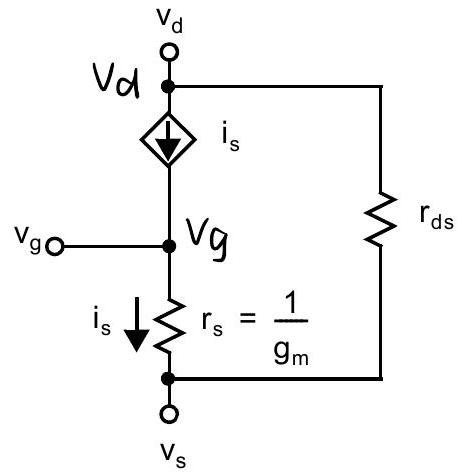
\includegraphics[max width=\textwidth, center]{2024_10_31_60860e27b87166db2267g-054}

Fig. 1.20 The small-signal, low-frequency T model for an active MOS transistor (the body effect is not modelled).

An alternate low-frequency model, known as a T model, is shown in Fig. 1.20. This T model can often result in simpler equations and is most often used by experienced designers for a quick analysis. At first glance, it might appear that this model allows for nonzero gate current, but a quick check confirms that the drain current must always equal the source current, and, therefore, the gate current must always be zero. For this reason, when using the T model, one assumes from the beginning that the gate current is zero.

\section*{EXAMPLE 1.12}
Find the T model parameter, $r_{\mathrm{s}}$, for the transistor in Example 1.10.

\section*{Solution}
The value of $r_{s}$ is simply the inverse of $g_{m}$, resulting in

$$
r_{s}=\frac{1}{g_{m}}=\frac{1}{0.94 \times 10^{-3}}=1.06 \mathrm{k} \Omega
$$

The value of $r_{\mathrm{ds}}$ remains the same, either $35 \mathrm{k} \Omega$ or $41 \mathrm{k} \Omega$ depending on the drain-source voltage.

\subsection*{1.2.7 High-Frequency Small-Signal Modelling in the Active Region}
A high-frequency model of a MOSFET in the active region is shown in Fig. 1.21. Most of the capacitors in the small-signal model are related to the physical transistor. Shown in Fig. 1.22 is a cross section of a MOS transistor, where the parasitic capacitances are shown at the appropriate locations. The largest capacitor in Fig. 1.22 is $\mathrm{C}_{\mathrm{gs}}$. This capacitance is primarily due to the change in channel charge as a result of a change in $\mathrm{V}_{\mathrm{GS}}$. It can be shown [Tsividis, 1987] that $\mathrm{C}_{\mathrm{gs}}$ is approximately given by


\begin{equation*}
\mathrm{C}_{\mathrm{gs}} \cong \frac{2}{3} \mathrm{WLC}_{\mathrm{ox}} \tag{1.89}
\end{equation*}


\begin{center}
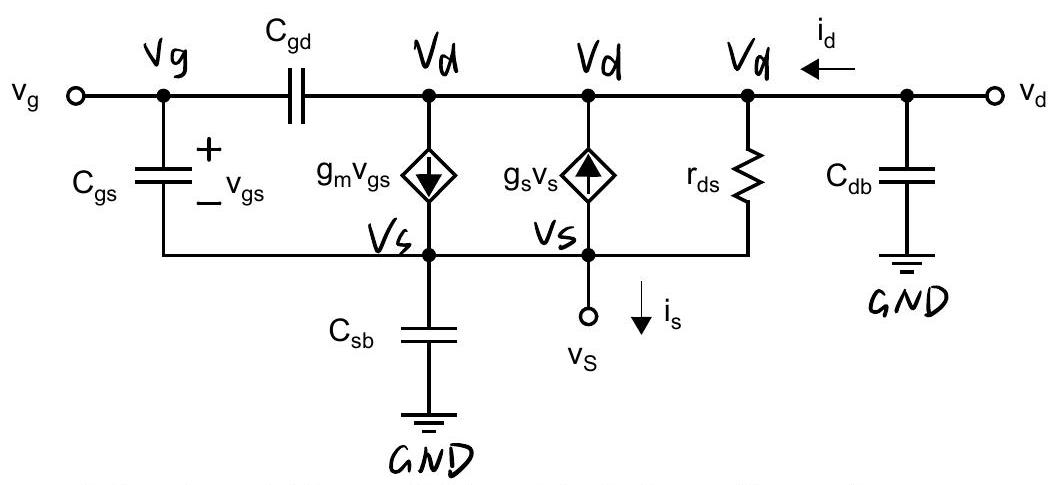
\includegraphics[max width=\textwidth]{2024_10_31_60860e27b87166db2267g-055}
\end{center}

Fig. 1.21 The small-signal model for a MOS transistor in the active region.

When accuracy is important, an additional term should be added to (1.89) to take into account the overlap between the gate and source junction, which should include the fringing capacitance (fringing capacitance is due to boundary effects). This additional component is given by


\begin{equation*}
C_{o v}=W L_{o v} C_{o x} \tag{1.90}
\end{equation*}


where $L_{\mathrm{ov}}$ is the effective overlap distance and is usually empirically derived ${ }^{15}$. Thus,


\begin{equation*}
\mathrm{C}_{\mathrm{gs}}=\frac{2}{3} \mathrm{WLC}_{\mathrm{ox}}+\mathrm{C}_{\mathrm{ov}} \tag{1.91}
\end{equation*}


Key Point: In a MOSFET, the largest parasitic capacitance is $\mathrm{C}_{\mathrm{gs} \text { s }}$, proportional to gate area WL and via $\mathrm{C}_{\mathrm{ox}}$ inversely proportional to oxide thickness.\\
when higher accuracy is needed.\\
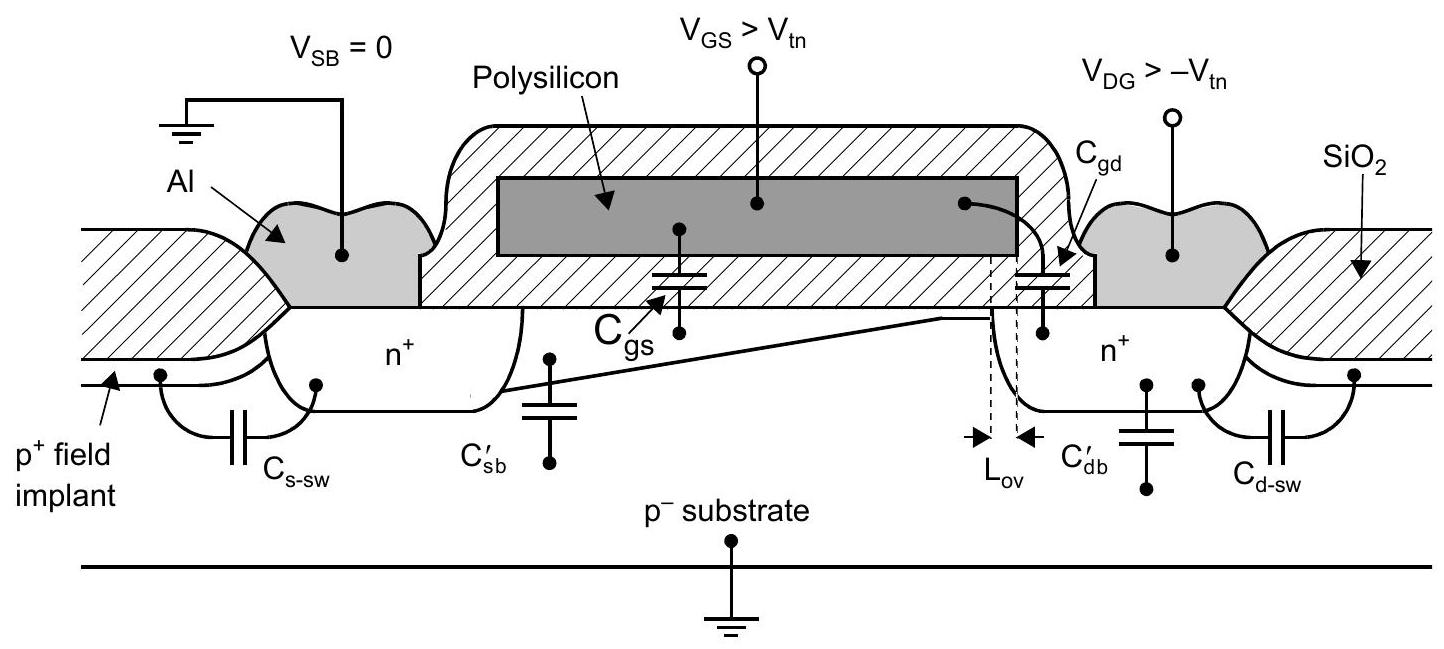
\includegraphics[max width=\textwidth, center]{2024_10_31_60860e27b87166db2267g-055(1)}

Fig. 1.22 A cross section of an n-channel MOS transistor showing the small-signal capacitances.\\
15. Part of the overlap capacitance is due to fringe electric fields, and therefore $\mathrm{L}_{\mathrm{ov}}$ is usually taken larger than its actual physical overlap to more accurately give an effective value for overlap capacitances.

The next largest capacitor in Fig. 1.22 is $\mathrm{C}_{\text {sb }}$, the capacitor between the source and the substrate. This capacitor is due to the depletion capacitance of the reverse-biased source junction, and it includes the channel-to-bulk capacitance (assuming the transistor is on). Its size is given by


\begin{equation*}
C_{s b}^{\prime}=\left(A_{s}+A_{c h}\right) C_{j s} \tag{1.92}
\end{equation*}


where $A_{s}$ is the area of the source junction, $A_{c h}$ is the area of the channel (i.e., $W L$ ) and $C_{j s}$ is the depletion capacitance of the source junction, given by


\begin{equation*}
\mathrm{C}_{\mathrm{is}}=\frac{\mathrm{C}_{\mathrm{j} 0}}{\sqrt{1+\frac{\mathrm{V}_{\mathrm{SB}}}{\Phi_{0}}}} \tag{1.93}
\end{equation*}


Note that the total area of the effective source includes the original area of the junction (when no channel is present) plus the effective area of the channel.

The depletion capacitance of the drain is smaller because it does not include the channel area. Here, we have


\begin{equation*}
\mathrm{C}_{\mathrm{db}}^{\prime}=\mathrm{A}_{\mathrm{d}} \mathrm{C}_{\mathrm{jd}} \tag{1.94}
\end{equation*}


where


\begin{equation*}
\mathrm{C}_{\mathrm{jd}}=\frac{\mathrm{C}_{\mathrm{j} 0}}{\sqrt{1+\frac{\mathrm{V}_{\mathrm{DB}}}{\Phi_{0}}}} \tag{1.95}
\end{equation*}


and $A_{d}$ is the area of the drain junction.\\
The capacitance $\mathrm{C}_{\mathrm{gd}}$, sometimes called the Miller capacitance, is important when there is a large voltage gain between gate and drain. It is primarily due to the overlap between the gate and the drain and fringing capacitance. Its value is given by


\begin{equation*}
C_{g d}=C_{o x} W L_{o v} \tag{1.96}
\end{equation*}


Key Point: The gate-drain capacitance $\mathrm{C}_{\mathrm{gd}}$ also known as the Miller capacitance, is due to physical overlap of the gate and drain regions as well as fringing fields. It is especially important when there is a large voltage gain between gate and drain.\\
where, once again, $\mathrm{L}_{\mathrm{ov}}$ is usually empirically derived.\\
Two other capacitors are often important in integrated circuits. These are the source and drain sidewall capacitances, $\mathrm{C}_{\mathrm{s} \text {-sw }}$ and $\mathrm{C}_{\mathrm{d} \text {-sw }}$. These capacitances can be large because of some highly doped $\mathrm{p}^{+}$regions under the thick field oxide called field implants. The major reason these regions exist is to ensure there is no leakage current between transistors. Because they are highly doped and they lie beside the highly doped source and drain junctions, the sidewall capacitances can result in large additional capacitances that must be taken into account in determining $C_{s b}$ and $C_{d b}$. The sidewall capacitances are especially important in modern technologies as dimensions shrink. For the source, the sidewall capacitance is given by


\begin{equation*}
C_{s-s w}=P_{s} C_{j-s w} \tag{1.97}
\end{equation*}


where $P_{s}$ is the length of the perimeter of the source junction, excluding the side adjacent to the channel, and


\begin{equation*}
C_{j-s w}=\frac{C_{j-s w 0}}{\sqrt{1+\frac{V_{S B}}{\Phi_{0}}}} \tag{1.98}
\end{equation*}


It should be noted that $\mathrm{C}_{\mathrm{j} \text {-sw } 0}$, the sidewall capacitance per unit length at $0-\mathrm{V}$ bias voltage, can be quite large because the field implants are heavily doped.

The situation is similar for the drain sidewall capacitance, $\mathrm{C}_{\mathrm{d} \text {-sw }}$,


\begin{equation*}
C_{d-s w}=P_{d} C_{j-s w} \tag{1.99}
\end{equation*}


where $P_{d}$ is the drain perimeter excluding the portion adjacent to the gate.\\
Finally, the source-bulk capacitance, $\mathrm{C}_{\mathrm{sb}}$, is given by


\begin{equation*}
C_{s b}=C_{s b}^{\prime}+C_{s-\mathrm{sw}} \tag{1.100}
\end{equation*}


with the drain-bulk capacitance, $\mathrm{C}_{\mathrm{db}}$, given by


\begin{equation*}
C_{d b}=C_{d b}^{\prime}+C_{d-s w} \tag{1.101}
\end{equation*}


\section*{EXAMPLE 1.13}
An n -channel transistor is modelled as having the following capacitance parameters: $\mathrm{C}_{\mathrm{j}}=2.4 \times 10^{-4} \mathrm{pF} /(\mu \mathrm{m})^{2}$, $\mathrm{C}_{\mathrm{j} \text {-sw }}=2.0 \times 10^{-4} \mathrm{pF} / \mu \mathrm{m}, \mathrm{C}_{\mathrm{ox}}=1.9 \times 10^{-3} \mathrm{pF} /(\mu \mathrm{m})^{2}, \mathrm{C}_{\mathrm{ov}}=2.0 \times 10^{-4} \mathrm{pF} / \mu \mathrm{m}$. Find the capacitances $\mathrm{C}_{\mathrm{gs}}$, $\mathrm{C}_{\mathrm{gd},} \mathrm{C}_{\mathrm{db} \text {, and }} \mathrm{C}_{\mathrm{sb}}$ for a transistor having $\mathrm{W}=100 \mu \mathrm{~m}$ and $\mathrm{L}=2 \mu \mathrm{~m}$. Assume the source and drain junctions extend $4 \mu \mathrm{~m}$ beyond the gate, so that the source and drain areas are $A_{s}=A_{d}=400(\mu \mathrm{~m})^{2}$ and the perimeter of each is $P_{s}=P_{d}=108 \mu \mathrm{~m}$.

\section*{Solution}
We calculate the various capacitances as follows:

$$
\begin{gathered}
C_{g s}=\left(\frac{2}{3}\right) W L C_{o x}+C_{o v} \times W=0.27 \mathrm{pF} \\
C_{g d}=C_{o v} \times W=0.02 \mathrm{pF} \\
C_{s b}=C_{j}\left(A_{s}+W L\right)+\left(C_{j-s w} \times P_{s}\right)=0.17 \mathrm{pF} \\
C_{d b}=\left(C_{j} \times A_{d}\right)+\left(C_{j-s w} \times P_{d}\right)=0.12 \mathrm{pF}
\end{gathered}
$$

Note that the source-bulk and drain-bulk capacitances are significant compared to the gate-source capacitance, in this case $1-2 \mathrm{fF} / \mu \mathrm{m}$ width compared with $2.7 \mathrm{fF} / \mu \mathrm{m}$ for $\mathrm{C}_{\mathrm{gs}}$. Thus, for high-speed circuits, it is important to keep the areas and perimeters of drain and source junctions as small as possible (possibly by sharing junctions between transistors, as seen in the next chapter).

\subsection*{1.2.8 Small-Signal Modelling in the Triode and Cutoff Regions}
The low-frequency, small-signal model of a MOS transistor in the triode region (which is sometimes referred to as the linear region) is a voltage-controlled resistor with $\mathrm{V}_{\mathrm{GS}}$, or equivalently $\mathrm{V}_{\text {eff }}$, used as the control terminal. Using (1.61), the large-signal equation for $I_{D}$ in the triode region,


\begin{equation*}
\mathrm{I}_{\mathrm{D}}=\mu_{\mathrm{n}} \mathrm{C}_{\mathrm{ox}}\left(\frac{\mathrm{~W}}{\mathrm{~L}}\right)\left[\left(\mathrm{V}_{\mathrm{GS}}-\mathrm{V}_{\mathrm{tn}}\right) \mathrm{V}_{\mathrm{DS}}-\frac{\mathrm{V}_{\mathrm{DS}}^{2}}{2}\right] \tag{1.102}
\end{equation*}


results in


\begin{equation*}
\frac{1}{r_{d s}}=g_{d s}=\frac{\partial I_{D}}{\partial V_{D S}}=\mu_{n} C_{o x}\left(\frac{W}{L}\right)\left(V_{G S}-V_{t n}-V_{D S}\right) \tag{1.103}
\end{equation*}


where $r_{d s}$ is the small-signal drain-source resistance (and $g_{d s}$ is the conductance). For the common case of $V_{D S}$ near zero, we have


\begin{equation*}
g_{\mathrm{ds}}=\frac{1}{\mathrm{r}_{\mathrm{ds}}}=\mu_{\mathrm{n}} \mathrm{C}_{\mathrm{ox}}\left(\frac{\mathrm{~W}}{\mathrm{~L}}\right)\left(\mathrm{V}_{\mathrm{Gs}}-\mathrm{V}_{\mathrm{tn}}\right)=\mu_{\mathrm{n}} \mathrm{C}_{\mathrm{ox}}\left(\frac{\mathrm{~W}}{\mathrm{~L}}\right) \mathrm{V}_{\mathrm{eff}} \tag{1.104}
\end{equation*}


which is similar to the $I_{D}$-versus- $V_{D S}$ relationship given earlier in (1.56).

\section*{EXAMPLE 1.14}
For the transistor of Example 1.10, find the triode model parameters when $\mathrm{V}_{\mathrm{DS}}$ is near zero.

\section*{Solution}
From (1.104), we have

$$
g_{\mathrm{ds}}=270 \times 10^{-6} \times\left(\frac{5}{0.5}\right) \times 0.35=0.94 \mathrm{~mA} / \mathrm{V}
$$

Note that this conductance value is the same as the transconductance of the transistor, $\mathrm{g}_{\mathrm{m}}$, in the active region. The resistance, $\mathrm{r}_{\mathrm{ds}}$, is simply $1 / \mathrm{g}_{\mathrm{ds}}$, resulting in $\mathrm{r}_{\mathrm{ds}}=1.06 \mathrm{k} \Omega$.

The accurate small-signal modelling of the high-frequency operation of a transistor in the triode region is nontrivial (even with the use of a computer simulation). A moderately accurate model is shown in Fig. 1.23, where the gate-to-channel capacitance and the channel-to-substrate capacitance are modelled as distributed elements. However, the I-V relationships of the distributed RC elements are highly nonlinear because the junction capacitances of the source and drain are nonlinear depletion capacitances, as is the channel-to-substrate capacitance. Also, if $\mathrm{V}_{\mathrm{DS}}$ is not small, then the channel resistance per unit length should increase as one moves closer to the drain. This model is much too complicated for use in hand analysis.\\
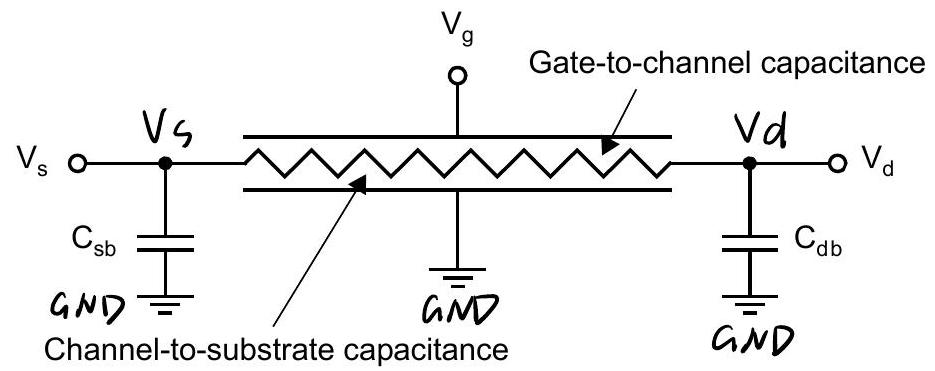
\includegraphics[max width=\textwidth, center]{2024_10_31_60860e27b87166db2267g-058}

Fig. 1.23 A distributed RC model for a transistor in the triode region.

A simplified model often used for small $\mathrm{V}_{\mathrm{DS}}$ is shown in Fig. 1.24, where the resistance, $r_{d s}$, is given by (1.104). Here, the gate-to-channel capacitance has been evenly divided between the source and drain nodes,


\begin{equation*}
C_{g s}=C_{g d}=\frac{A_{c h} C_{0 x}}{2}=\frac{W_{L C} C_{0 x}}{2} \tag{1.105}
\end{equation*}


Note that this equation ignores the gate-to-junction overlap capacitances, as given by (1.90), which should be taken into account when accuracy is very important. The channel-tosubstrate capacitance has also been divided in half and shared between the source and drain junctions. Each of these capacitors should be added to the junction-to-substrate capacitance and the junction-sidewall capacitance at the appropriate node.\\
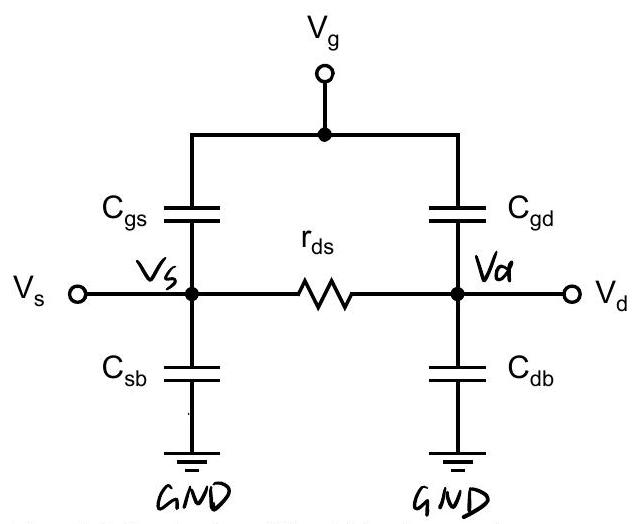
\includegraphics[max width=\textwidth, center]{2024_10_31_60860e27b87166db2267g-059}

Fig. 1.24 A simplified triode-region model valid for small $V_{D S}$.

Thus, we have


\begin{equation*}
C_{s b-0}=C_{j 0}\left(A_{s}+\frac{A_{c h}}{2}\right)+C_{j-s w 0} P_{s} \tag{1.106}
\end{equation*}


and


\begin{equation*}
C_{d b-0}=C_{j 0}\left(A_{d}+\frac{A_{c h}}{2}\right)+C_{j-s w 0} P_{d} \tag{1.107}
\end{equation*}


Also,


\begin{equation*}
\mathrm{C}_{\mathrm{sb}}=\frac{\mathrm{C}_{\mathrm{sb}-0}}{\sqrt{1+\frac{\mathrm{V}_{\mathrm{sb}}}{\Phi_{0}}}} \tag{1.108}
\end{equation*}


and


\begin{equation*}
\mathrm{C}_{\mathrm{db}}=\frac{\mathrm{C}_{\mathrm{db}-0}}{\sqrt{1+\frac{\mathrm{V}_{\mathrm{db}}}{\Phi_{0}}}} \tag{1.109}
\end{equation*}


It might be noted that $\mathrm{C}_{\mathrm{sb}}$ is often comparable in size to $\mathrm{C}_{\mathrm{gs}}$ due to its larger area and the sidewall capacitance.\\
When the transistor turns off, the small-signal model changes considerably. A reasonable model is shown in Fig. 1.25. Perhaps the biggest difference is that $r_{d s}$ is now infinite. Another major difference is that $C_{g s}$ and $C_{g d}$ are now much smaller. Since the channel has disappeared, these capacitors are now due to only overlap and fringing capacitance. Thus, we have


\begin{equation*}
C_{g s}=C_{g d}=W L_{o v} C_{o x} \tag{1.110}
\end{equation*}


However, the reduction of $\mathrm{C}_{g \mathrm{~s}}$ and $\mathrm{C}_{\mathrm{gd}}$ does not mean that the total gate capacitance is necessarily smaller. We now have a "new" capacitor, $\mathrm{C}_{\mathrm{gb}}$, which is the gate-to-substrate capacitance. This capacitor is highly nonlinear and dependent on the gate voltage. If the gate voltage has been very negative for some time and the gate is accumulated, then we have


\begin{equation*}
C_{g b}=A_{c h} C_{o x}=W L C_{o x} \tag{1.111}
\end{equation*}


\begin{center}
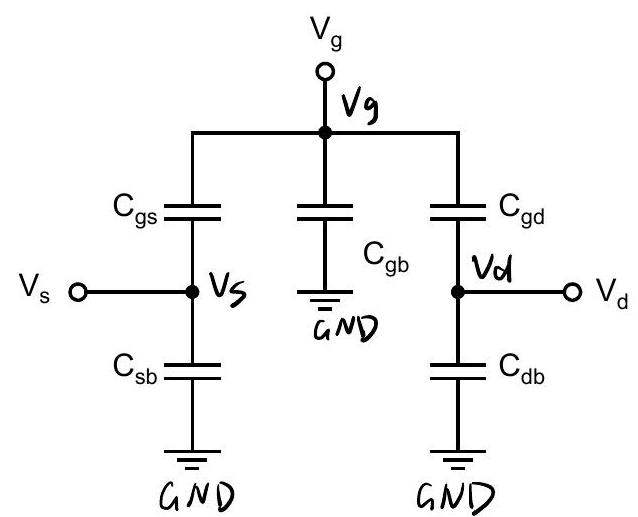
\includegraphics[max width=\textwidth]{2024_10_31_60860e27b87166db2267g-060}
\end{center}

Fig. 1.25 A small-signal model for a MOSFET that is turned off.

If the gate-to-source voltage is around 0 V , then $\mathrm{C}_{\mathrm{gb}}$ is equal to $\mathrm{C}_{\mathrm{ox}}$ in series with the channel-to-bulk depletion capacitance and is considerably smaller, especially when the substrate is lightly doped. Another case where $\mathrm{C}_{\mathrm{gb}}$ is small is just after a transistor has been turned off, before the channel has had time to accumulate. Because of the complicated nature of correctly modelling $\mathrm{C}_{\mathrm{gb}}$ when the transistor is turned off, equation (1.111) is usually used for hand analysis as a worst-case estimate.

The capacitors $\mathrm{C}_{\mathrm{sb}}$ and $\mathrm{C}_{\mathrm{db}}$ are also smaller when the channel is not present. We now have


\begin{equation*}
\mathrm{C}_{\mathrm{sb}-0}=\mathrm{A}_{\mathrm{s}} \mathrm{C}_{\mathrm{j} 0} \tag{1.112}
\end{equation*}


and


\begin{equation*}
C_{d b-0}=A_{d} C_{j 0} \tag{1.113}
\end{equation*}


\subsection*{1.2.9 Analog Figures of Merit and Trade-offs}
With so many device constants and small-signal model parameters, it is sometimes useful to have a single number that captures some key aspect of transistor performance. Two such figures of merit are considered in this section: intrinsic gain, which relates to the transistor's low-frequency small-signal performance; and intrinsic speed, related to the transistor's high-frequency small-signal performance.

The intrinsic gain of a transistor is a measure of the maximum possible low-frequency small-signal voltage gain it can provide. The voltage gain of a transistor is generally maximized by operating it in the active mode with the source terminal (small-signal) grounded, the input applied to the gate, and the output observed at the drain terminal, as shown in Fig. 1.26(a). In order to maximize gain, an ideal current source is used to provide the drain current so that the only load the drain terminal sees is the transistor itself. Measured in this way, the intrinsic gain is closely related to the gain provided by several important singlestage amplifier stages discussed in later sections, such as common-source amplifiers and differential pairs with active loads.\\
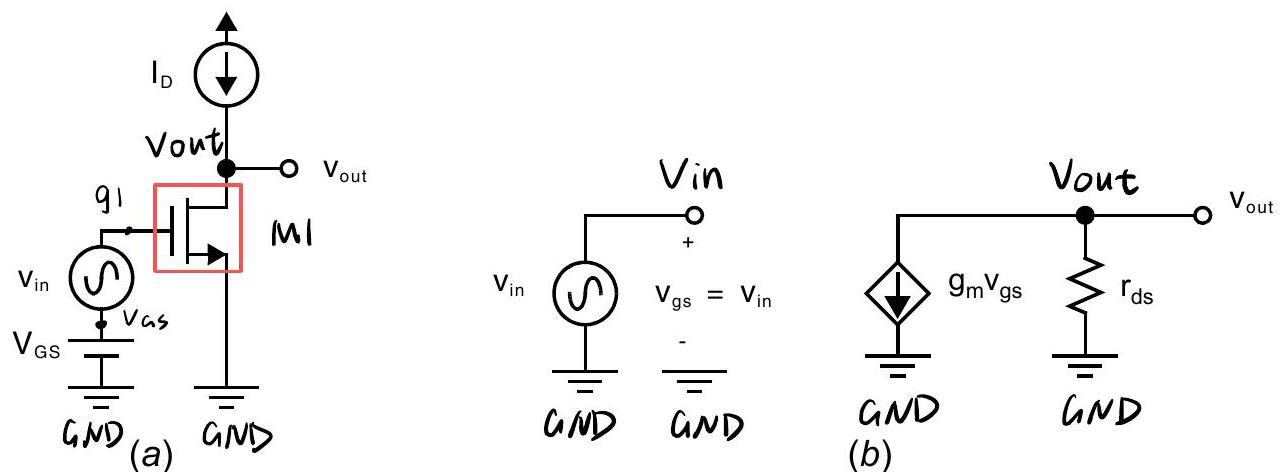
\includegraphics[max width=\textwidth, center]{2024_10_31_60860e27b87166db2267g-060(1)}\\
(b)

Fig. 1.26 The circuit used to characterize transistor intrinsic gain: a) complete circuit; b) dc smallsignal equivalent.

The small-signal equivalent circuit at dc simplifies to that shown in Fig. 1.26(b). The transistor's intrinsic gain is therefore,


\begin{equation*}
A_{i}=\left|\frac{v_{\text {out }}}{v_{\text {in }}}\right|=g_{m} r_{\text {ds }} \tag{1.114}
\end{equation*}


Substituting the expressions for $g_{m}$ from equation (1.78) and $r_{d s}$ from (1.86) gives a simple expression for transistor intrinsic gain dependent on only a few device parameters.


\begin{equation*}
A_{i} \cong \frac{2 I_{D}}{V_{\text {eff }}} \cdot \frac{1}{\lambda I_{D}}=\frac{2}{\lambda V_{\text {eff }}} \tag{1.115}
\end{equation*}


The intrinsic gain in the active mode will be somewhat larger than this because (1.115) assumes $r_{d s} \cong 1 / \lambda I_{D}$ whereas in fact $r_{d s} \cong 1 / \lambda I_{D, \text { sat }}$ which is somewhat larger.

This reveals two important general conclusions about analog design: first, that to maximize dc gain, transistors should be operated with small values of $\mathrm{V}_{\text {eff }}$; second, since $\lambda$ is inversely proportional to gate length L , as shown in equation (1.87), intrinsic gain is maximized by taking long gate lengths.

\section*{EXAMPLE 1.15}
Calculate the intrinsic gain of the transistor in Example 1.10 when in active mode.

\section*{Solution}
The intrinsic gain is obtained by substituting the values for $g_{m}$ and $r_{d s}$ calculated in Example 1.10 into (1.114).

$$
A_{i}=g_{m} r_{d s}=32.9
$$

This is the largest voltage gain this single transistor can achieve under these operating bias conditions.

The unity-gain frequency of a transistor, $\mathrm{f}_{\mathrm{t}}$, is intended to provide some measure of the maximum operating frequency at which a transistor might prove useful. It is the most common (though not the only) measure of transistor intrinsic speed. As with intrinsic gain, $f_{t}$ is measured in the common-source configuration because of its broad relevance to both analog and digital design. An idealized measurement setup is shown in Fig. 1.27(a). Bias\\
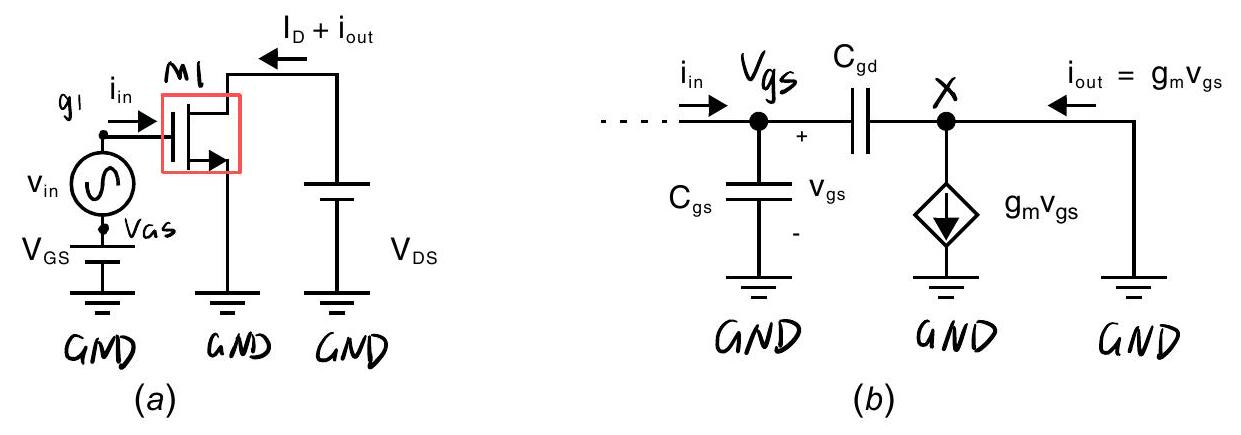
\includegraphics[max width=\textwidth, center]{2024_10_31_60860e27b87166db2267g-061}

Fig. 1.27 The circuit used to characterize transistor intrinsic speed: (a) complete circuit; (b) high-frequency small-signal equivalent.\\
voltages $\mathrm{V}_{\mathrm{GS}}$ and $\mathrm{V}_{\mathrm{DS}}$ are applied to the gate and drain, respectively. A sinusoidal signal, $\mathrm{v}_{\mathrm{in}}$, with very small amplitude is superimposed on the gate voltage. This gives rise to small sinusoidal currents: $\mathrm{i}_{\mathrm{in}}$ which charges and discharges the gate capacitances in response to $v_{i n}$; and $i_{\text {out }}$ which is a small signal current superimposed on the dc drain current, $\mathrm{I}_{\mathrm{D}}$. The unity-gain frequency is defined as the maximum frequency at which the amplitude of the output small-signal current, $\left|\mathrm{i}_{\text {out }}\right|$, exceeds that of the input current, $\left|\mathrm{i}_{\mathrm{in}}\right|$. Although conceptually simple, this measurement is notoriously difficult to perform in the lab since the frequencies involved are high and any parasitic capacitances in the measurement setup will influence the result.

A first-order analytical solution for the transistor $f_{t}$ follows straightforwardly from an analysis of the smallsignal equivalent circuit in Fig. 1.27(b), which is left as an exercise for the reader.


\begin{equation*}
\mathrm{f}_{\mathrm{t}} \approx \frac{\mathrm{~g}_{\mathrm{m}}}{2 \pi\left(\mathrm{C}_{\mathrm{gs}}+\mathrm{C}_{\mathrm{gd}}\right)} \tag{1.116}
\end{equation*}


Although the accuracy of (1.116) is limited, we will adopt this expression as our definition of $f_{t}$ because it is compact and closely related to the bandwidth of many important circuits we shall study.

Clearly, transistor intrinsic speed is dependent on biasing. Substituting (1.74) and (1.89) into (1.116) and assuming $\mathrm{C}_{g s}$ » $\mathrm{C}_{\mathrm{gd}}$ gives the following approximate result for the unity-gain frequency of a transistor:


\begin{equation*}
f_{t} \approx \frac{\mu_{n} C_{o x}(W / L) V_{\text {eff }}}{2 \pi C_{o x} W(2 / 3) L}=\frac{3 \mu_{n} V_{\text {eff }}}{4 \pi L^{2}} \tag{1.117}
\end{equation*}


Key Point: For operation with high gain, transistors should have long gate lengths and be biased with low $\mathrm{V}_{\text {eff }}$ For high speed, the opposite is desirable: small L and high $\mathrm{V}_{\text {eff }}$

As with intrinsic gain, some important fundamental conclusions about analog design are revealed by (1.117). First, for operation at high-speed, device parasitic capacitances should be minimized, which implies minimizing the device gate length, L . Second, speed is maximized by biasing with high values of $\mathrm{V}_{\text {eff }}$. These requirements are in direct conflict with those outlined for maximizing transistor intrinsic gain.

\subsection*{1.3 DEVICE MODEL SUMMARY}
As a useful aid, all of the equations for the large-signal and small-signal modelling of diodes and MOS transistors, along with values for the various constants, are listed in the next few pages.

\subsection*{1.3.1 Constants}
\begin{center}
\begin{tabular}{|l|l|}
\hline
$\mathrm{q}=1.602 \times 10^{-19} \mathrm{C}$ & $\mathrm{k}=1.38 \times 10^{-23} \mathrm{JK}^{-1}$ \\
\hline
$\mathrm{n}_{\mathrm{i}}=1.1 \times 10^{16} \mathrm{carriers} / \mathrm{m}^{3}$ at $\mathrm{T}=300{ }^{\circ} \mathrm{K}$ & $\varepsilon_{0}=8.854 \times 10^{-12} \mathrm{~F} / \mathrm{m}$ \\
\hline
$\mathrm{K}_{\mathrm{ox}} \cong 3.9$ & $\mathrm{~K}_{\mathrm{s}} \cong 11.8$ \\
\hline
\end{tabular}
\end{center}

\subsection*{1.3.2 Diode Equations}
\section*{Reverse-Biased Diode (Abrupt Junction)}
\begin{center}
\begin{tabular}{|c|c|}
\hline
\( C_{j}=\frac{C_{j 0}}{\sqrt{1+\frac{V_{B}}{\Phi_{0}}}} \) & $\mathrm{Q}=2 \mathrm{C}_{\mathrm{j} 0} \Phi_{0} \sqrt{1+\frac{\mathrm{V}_{\mathrm{B}}}{\Phi_{0}}}$ \\
\hline
$\mathrm{C}_{\mathrm{j} 0}=\sqrt{\frac{\mathrm{q} \mathrm{K}_{\mathrm{s}} \varepsilon_{0}}{2 \Phi_{0}} \frac{\mathrm{~N}_{\mathrm{D}} \mathrm{N}_{\mathrm{A}}}{\mathrm{N}_{\mathrm{A}}+\mathrm{N}_{\mathrm{D}}}}$ & $\mathrm{C}_{\mathrm{j} 0}=\sqrt{\frac{\mathrm{q} \mathrm{K}_{\mathrm{s}} \varepsilon_{0} \mathrm{~N}_{\mathrm{D}}}{2 \Phi_{0}}}$ if $\mathrm{N}_{\mathrm{A}}>>\mathrm{N}_{\mathrm{D}}$ \\
\hline
\multicolumn{2}{|r|}{$\Phi_{0}=\frac{\mathrm{kT}}{\mathrm{q}} \ln \left(\frac{\mathrm{N}_{\mathrm{A}} \mathrm{N}_{\mathrm{D}}}{\mathrm{n}_{\mathrm{i}}^{2}}\right)$} \\
\hline
\end{tabular}
\end{center}

\section*{Forward-Biased Diode}
$$
\begin{gathered}
\hline I_{D}=I_{S} e^{v_{D} / V_{T}} \quad I_{S}=A_{D} q n_{i}^{2}\left(\frac{D_{n}}{L_{n} N_{A}}+\frac{D_{p}}{L_{p} N_{D}}\right) \\
\hline V_{T}=\frac{k T}{q} \cong 26 \mathrm{mV} \text { at } 300^{\circ} \mathrm{K} \\
\hline
\end{gathered}
$$

Small-Signal Model of Forward-Biased Diode\\
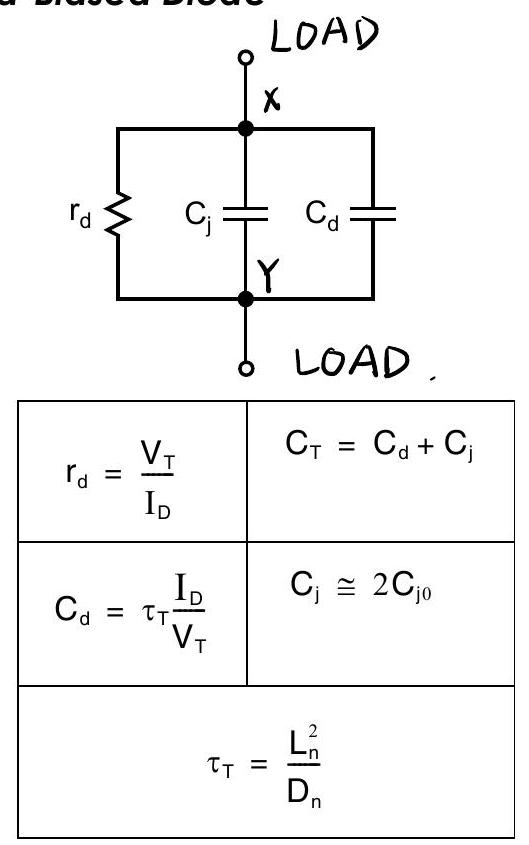
\includegraphics[max width=\textwidth, center]{2024_10_31_60860e27b87166db2267g-063}

\subsection*{1.3.3 MOS Transistor Equations}
The following equations are for $n$-channel devices-for p -channel devices, put negative signs in front of all voltages. These equations do not account for short-channel effects (i.e., $L<2 \mathrm{~L}_{\text {min }}$ ).

\section*{Triode Region ( $V_{G s}>V_{t n}, V_{D S} \leq V_{\text {eff }}$ )}
\begin{center}
\begin{tabular}{|c|c|}
\hline
\multicolumn{2}{|r|}{$\mathrm{I}_{\mathrm{D}}=\mu_{\mathrm{n}} \mathrm{C}_{\text {ox }}\left(\frac{\mathrm{W}}{\mathrm{L}}\right)\left[\left(\mathrm{V}_{\mathrm{GS}}-\mathrm{V}_{\mathrm{tn}}\right) \mathrm{V}_{\mathrm{DS}}-\frac{\mathrm{V}_{\mathrm{DS}}^{2}}{2}\right]$} \\
\hline
$\mathrm{V}_{\text {eff }}=\mathrm{V}_{\mathrm{GS}}-\mathrm{V}_{\mathrm{tn}}$ & $\mathrm{V}_{\mathrm{tn}}=\mathrm{V}_{\mathrm{tn-0}}+\gamma\left(\sqrt{\mathrm{V}_{\mathrm{SB}}+2 \phi_{\mathrm{F}}}-\sqrt{2 \phi_{\mathrm{F}}}\right)$ \\
\hline
$\phi_{\mathrm{F}}=\frac{\mathrm{kT}}{\mathrm{q}} \ln \left(\frac{\mathrm{N}_{\mathrm{A}}}{\mathrm{n}_{\mathrm{i}}}\right)$ & \( \gamma=\frac{\sqrt{2 \mathrm{qK}_{\mathrm{s}} \varepsilon_{0} \mathrm{~N}_{\mathrm{A}}}}{\mathrm{C}_{\mathrm{ox}}} \) \\
\hline
 & \( \mathrm{C}_{\mathrm{ox}}=\frac{\mathrm{K}_{\mathrm{ox}} \varepsilon_{0}}{\mathrm{t}_{\mathrm{ox}}} \) \\
\hline
\end{tabular}
\end{center}

Small-Signal Model in Triode Region (for $V_{D s} \ll V_{\text {eff }}$ )\\
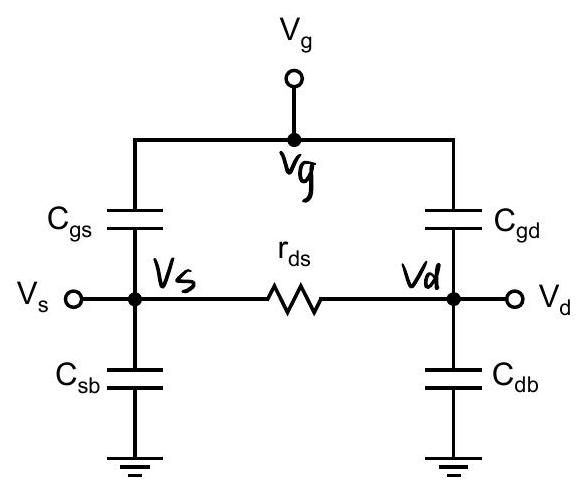
\includegraphics[max width=\textwidth, center]{2024_10_31_60860e27b87166db2267g-064}

\begin{center}
\begin{tabular}{|c|c|}
\hline
\multicolumn{2}{|c|}{\multirow[t]{2}{*}{\(
r_{d s}=\frac{1}{\mu_{n} C_{o x}\left(\frac{W}{L}\right) V_{\text {eff }}}
\)}} \\
\hline
 &  \\
\hline
$\mathrm{C}_{\mathrm{gd}}=\mathrm{C}_{\mathrm{gs}} \cong \frac{1}{2} \mathrm{WLC}_{\mathrm{ox}}+\mathrm{WL}_{\mathrm{ov}} \mathrm{C}_{\mathrm{ox}}$ & \( C_{s b}=C_{d b}=\frac{C_{j 0}\left(A_{s}+W L / 2\right)}{\sqrt{1+\frac{V_{s b}}{\Phi_{0}}}} \) \\
\hline
\end{tabular}
\end{center}

Active (or Pinch-Off) Region ( $V_{G s}>V_{t n}, V_{D s} \geq V_{\text {eff }}$ )

\begin{center}
\begin{tabular}{|c|}
\hline
$\mathrm{I}_{\mathrm{D}}=\frac{1}{2} \mu_{\mathrm{n}} \mathrm{C}_{\mathrm{ox}} \frac{\mathrm{W}}{\mathrm{L}}\left(\mathrm{V}_{\mathrm{GS}}-\mathrm{V}_{\mathrm{tn}}\right)^{2}\left[1+\lambda\left(\mathrm{V}_{\mathrm{DS}}-\mathrm{V}_{\mathrm{eff}}\right)\right]$ \\
\hline
$\lambda \propto \frac{1}{\mathrm{~L} \sqrt{\mathrm{~V}_{\mathrm{DS}}-\mathrm{V}_{\text {eff }}+\Phi_{0}}} \quad \mathrm{~V}_{\mathrm{tn}}=\mathrm{V}_{\mathrm{tn}-0}+\gamma\left(\sqrt{V_{\mathrm{SB}}+2 \phi_{\mathrm{F}}}-\sqrt{2 \phi_{\mathrm{F}}}\right)$ \\
\hline
$\mathrm{V}_{\text {eff }}=\mathrm{V}_{\mathrm{GS}}-\mathrm{V}_{\mathrm{tn}}=\sqrt{\frac{2 \mathrm{I}_{\mathrm{D}}}{\mu_{\mathrm{n}} \mathrm{C}_{\mathrm{ox}} \mathrm{W} / \mathrm{L}}}$ \\
\hline
\end{tabular}
\end{center}

Small-Signal Model (Active Region)\\
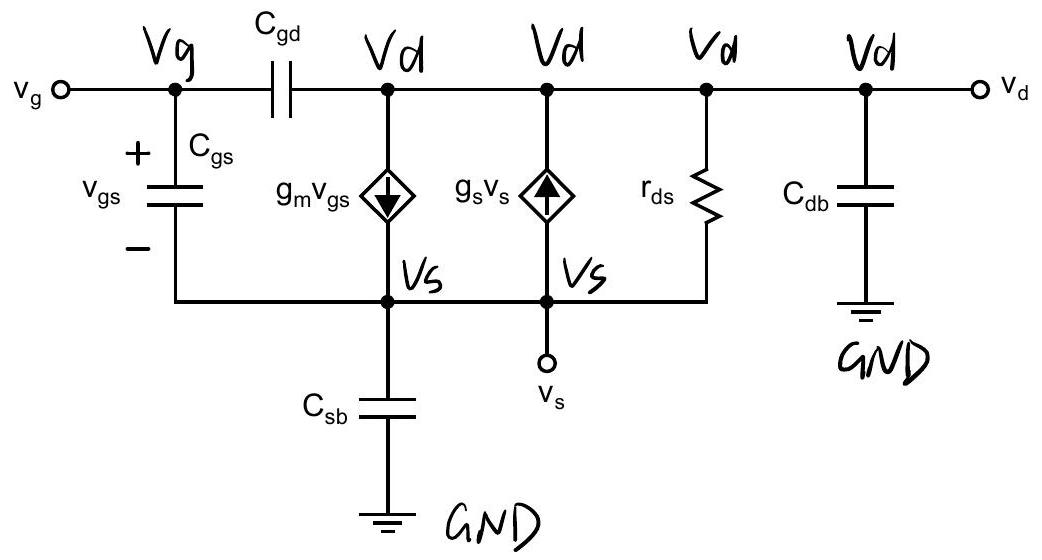
\includegraphics[max width=\textwidth, center]{2024_10_31_60860e27b87166db2267g-065}

\begin{center}
\begin{tabular}{|c|c|}
\hline
$g_{m}=\mu_{n} C_{o x}\left(\frac{W}{L}\right) V_{\text {eff }}$ & $g_{m}=\sqrt{2 \mu_{n} C_{o x}(W / L) I_{D}}$ \\
\hline
$g_{m}=\frac{2 I_{D}}{V_{\text {eff }}}$ & $g_{s}=\frac{\gamma g_{m}}{2 \sqrt{V_{S B}+\left|2 \phi_{F}\right|}}$ \\
\hline
$r_{d s}=\frac{1}{\lambda I_{D-\text { sat }}} \cong \frac{1}{\lambda I_{D}}$ & $g_{s} \cong 0.2 g_{m}$ \\
$\lambda=\frac{k_{r d s}}{2 L \sqrt{V_{D S}-V_{\text {eff }}+\Phi_{0}}}$ & $\mathrm{k}_{\mathrm{rds}}=\sqrt{\frac{2 \mathrm{~K}_{\mathrm{s}} \varepsilon_{0}}{q N_{A}}}$ \\
\hline
$C_{\mathrm{gs}}=\frac{2}{3} \mathrm{WLC}_{\mathrm{ox}}+\mathrm{WL}_{\mathrm{ov}} \mathrm{C}_{\mathrm{ox}}$ & $\mathrm{C}_{\mathrm{gd}}=\mathrm{WL}_{\mathrm{ov}} \mathrm{C}_{\mathrm{ox}}$ \\
\hline
\end{tabular}
\end{center}

\begin{center}
\begin{tabular}{|l|l|}
\hline
$C_{s b}=\left(A_{s}+W L\right) C_{i s}+P_{s} C_{i \cdot s w}$ & $C_{i s}=\frac{C_{j 0}}{\sqrt{1+V_{s B} / \Phi_{0}}}$ \\
\hline
$C_{d b}=A_{d} C_{i d}+P_{d} C_{j-s w}$ & $C_{i d}=\frac{C_{j 0}}{\sqrt{1+V_{D B} / \Phi_{0}}}$ \\
\hline
\end{tabular}
\end{center}

\subsection*{1.4 ADVANCED MOS MODELLING}
The square-law relationship between effective gate-source voltage and drain current expressed in equation (1.67) is only valid for active operation in strong inversion. For very small (and negative) values of $\mathrm{V}_{\text {eff }}$, MOS devices operate in weak inversion, also called subthreshold operation, where an exponential voltage-current relationship holds. For large values of $\mathrm{V}_{\text {eff }}$, a combination of effects give rise to a sub-square-law voltage-current relationship. Both are considered in this section. Other advanced modelling concepts that an analog microcircuit designer is likely to encounter are also covered, including parasitic resistances, short channel effects, and leakage currents.

\subsection*{1.4.1 Subthreshold Operation}
Key Point: In subthreshold operation, also called weak inversion, transistors obey an exponential voltagecurrent relationship instead of a square-law. Hence, a small but finite current flows even when $\mathrm{V}_{\mathrm{GS}}=0$.

The device equations presented for active or triode region MOS transistors in the preceding sections are all based on the assumption that $\mathrm{V}_{\text {eff }}$ is greater than about 100 mV and the device is in strong inversion. When this is not the case, the accuracy of the square-law equations is poor. For negative values of $\mathrm{V}_{\text {eff }}$, the transistor is in weak inversion and is said to be operating in the subthreshold region. In this regime, the dominant physical mechanism for conduction between drain and source is diffusion, not drift as in strong inversion, and the transistor is more accurately modelled by an exponential relationship between its control voltage (at the gate) and current, somewhat similar to a bipolar transistor. In the subthreshold region, the drain current is approximately given by an exponential relationship.


\begin{equation*}
I_{D(\text { sub -th })} \cong I_{D 0}\left(\frac{W}{L}\right) e^{\left(q V_{e f f} / n k T\right)} \tag{1.118}
\end{equation*}


where


\begin{align*}
\mathrm{n} & =\frac{\mathrm{C}_{\mathrm{ox}}+\mathrm{C}_{\mathrm{j} 0}}{\mathrm{C}_{\mathrm{ox}}} \approx 1.5  \tag{1.119}\\
\mathrm{I}_{\mathrm{D} 0} & =(\mathrm{n}-1) \mu_{\mathrm{n}} \mathrm{C}_{\mathrm{ox}}\left(\frac{\mathrm{kT}}{\mathrm{q}}\right)^{2} \tag{1.120}
\end{align*}


and it has been assumed that $\mathrm{V}_{\mathrm{S}}=0$ and $\mathrm{V}_{\mathrm{DS}}>75 \mathrm{mV}$. Not captured here is drain-induced barrier lowering, a short-channel effect that causes subthreshold current to also depend on drain-source voltage.

Plotting drain current on a logarithmic axis versus $\mathrm{V}_{\mathrm{GS}}$ in the subthreshold regime gives a straight line. The inverse of this slope, called the subthreshold slope and equal to $\ln (10) \cdot \mathrm{nkT} / \mathrm{q}=2.3 \mathrm{nkT} / \mathrm{q}$, is a measure of the voltage change in $\mathrm{V}_{\mathrm{GS}}$ required to effect an order-of-magnitude change in subthreshold drain current.

Also note that the current does not drop to zero even when $\mathrm{V}_{\mathrm{GS}}=0 \mathrm{~V}$. This residual drain current is called subthreshold leakage and considering equation (1.118) is given by


\begin{equation*}
I_{\text {off }}=I_{D o}\left(\frac{W}{L}\right) e^{\left(-q V_{t} / n k T\right)}=(n-1) \mu_{n} C_{o x}\left(\frac{W}{L}\right)\left(\frac{k T}{q}\right)^{2} e^{\left(-q V_{t} / n k T\right)} \tag{1.121}
\end{equation*}


Equation (1.121) reveals a complex temperature dependence due to the explicit inclusion of absolute temperature ( $T$ ), and due to the temperature dependence of carrier mobility $\left(\mu_{n}\right)$ and threshold voltage $\left(\mathrm{V}_{\mathrm{t}}\right)$. In general, subthreshold leakage increases significantly with temperature and is often a dominant source of power consumption in analog circuits that are temporarily powered down or in standby.

\section*{EXAMPLE 1.16}
A transistor has a subthreshold leakage current of $\mathrm{I}_{\text {off }}=10 \mathrm{nA}$ at 300 K . How much must $\mathrm{V}_{\text {eff }}$ decrease to reduce $\mathrm{I}_{\text {off }}$ to 1 nA ?

\section*{Solution}
From (1.118), it is evident that to decrease subthreshold drain current by a factor of 10 requires that $\mathrm{V}_{\text {eff }}$ decrease by $\ln (10) \cdot \mathrm{nkT} / \mathrm{q} \cong 90 \mathrm{mV}$ at room temperature. This can be achieved either by decreasing $\mathrm{V}_{\mathrm{GS}}$, or increasing $\mathrm{V}_{\mathrm{tn}}$.

The transconductance of a transistor in the subthreshold region is determined by taking the derivative of (1.118) with respect to $\mathrm{V}_{\mathrm{GS}}$ resulting in


\begin{equation*}
g_{m(\text { sub -th })}=\left(\frac{q}{n k T}\right) I{ }_{D 0}\left(\frac{W}{L}\right) e^{\left(q V_{\text {eff }} / n k T\right)}=\frac{q l_{D}}{n k T} \tag{1.122}
\end{equation*}


Note that for fixed drain current, $\mathrm{I}_{\mathrm{D}}$, the transconductance in subthreshold is independent of $\mathrm{V}_{\text {eff }}$. Normalizing the transconductance with respect to the drain current yields a constant value in subthreshold,


\begin{equation*}
\frac{g_{m(\text { sub-th })}}{I_{D(\text { sub-th })}}=\frac{q}{n k T} \tag{1.123}
\end{equation*}


As $\mathrm{V}_{\mathrm{Gs}}$ is increased well beyond $\mathrm{V}_{\mathrm{t}}$, the MOS device enters strong inversion and the transconductance then decreases in inverse proportion to $\mathrm{V}_{\text {eff }}$, as indicated by (1.78). Hence, for a fixed drain current, transconductance of a MOS device is maximized in the subthreshold region with the value given in (1.122). In other words, a targeted value of transconductance can be achieved with less drain current in the subthreshold region than in strong inversion. However, to achieve prac-

Key Point: For a fixed drain current, the smallsignal transconductance of a MOSdevice is maximized in subthreshold operation at a value of $\mathrm{g}_{\mathrm{m}}=\mathrm{qI}_{\mathrm{D}} / \mathrm{nkT}$.\\
tically useful values of transconductance in the subthreshold region requires a transistor with a very large aspect ratio, $\mathrm{W} / \mathrm{L}$. Such large aspect ratios generally imply large parasitic capacitances making very high-speed operation difficult. Therefore, subthreshold operation is useful primarily when speed can be sacrificed for lower drain currents and, hence, generally lower power consumption.

The transition between subthreshold and strong inversion is not abrupt. For a broad range of gate-source voltages, both diffusion and drift currents with comparable magnitudes exist making accurate device modeling in this region notoriously difficult. This is generally referred to as moderate inversion. To get a feel for what gate-source voltages imply moderate inversion, equate the expressions for $g_{m}$ in active mode (1.78) and $g_{m(\text { sub - th })}$ (1.122) and solve for $\mathrm{V}_{\text {eff }}$ resulting in


\begin{equation*}
V_{\text {eff }}=\frac{2 n k T}{q} \tag{1.124}
\end{equation*}


At room temperature and assuming $n \approx 1.5$, moderate inversion occurs around $V_{\text {eff }} \approx 75 \mathrm{mV}$, increasing to approximately 90 mV at 350 K . Hence, to ensure operation in strong inversion, prudent designers generally take $V_{\text {eff }}>100 \mathrm{mV}$.

\section*{EXAMPLE 1.17}
Estimate the value of n from the data for the NMOS device in Example 1.9 at $\mathrm{T}=300 \mathrm{~K}$.

\section*{Solution}
The logarithmic plot of $\mathrm{I}_{\mathrm{D}}$ versus $\mathrm{V}_{\mathrm{GS}}$ in Fig. 1.28(a) has a slope equal to ( 2.3 nkT )/q which in this case can be used to estimate n . The dashed line shows a reasonable fit with $\mathrm{n}=1.6$. This estimate can be confirmed by looking at the plot of $\mathrm{g}_{\mathrm{m}} / \mathrm{I}_{\mathrm{D}}$ also on Fig. $1.28(\mathrm{~b})$, which should reach a maximum of $\mathrm{q} / \mathrm{nkT}$ in subthreshold. Again, the dashed line with $\mathrm{n}=1.6$ is a reasonable approximation. Also shown on that plot is the result for the squarelaw model based on (1.78) based on the threshold voltage of $\mathrm{V}_{\mathrm{tn}} \cong 0.45 \mathrm{~V}$ obtained in Example 1.9. Note that the two regions intersect at $\mathrm{V}_{\mathrm{GS}}=\mathrm{V}_{\mathrm{tn}}+2 \mathrm{nkT} / \mathrm{q}$.

\subsection*{1.4.2 Mobility Degradation}
Transistors subjected to large electric fields experience a degradation in the effective mobility of their carriers. Large lateral electric fields, as shown in Fig. 1.29 for an NMOS device, accelerate carriers in the channel up to a\\
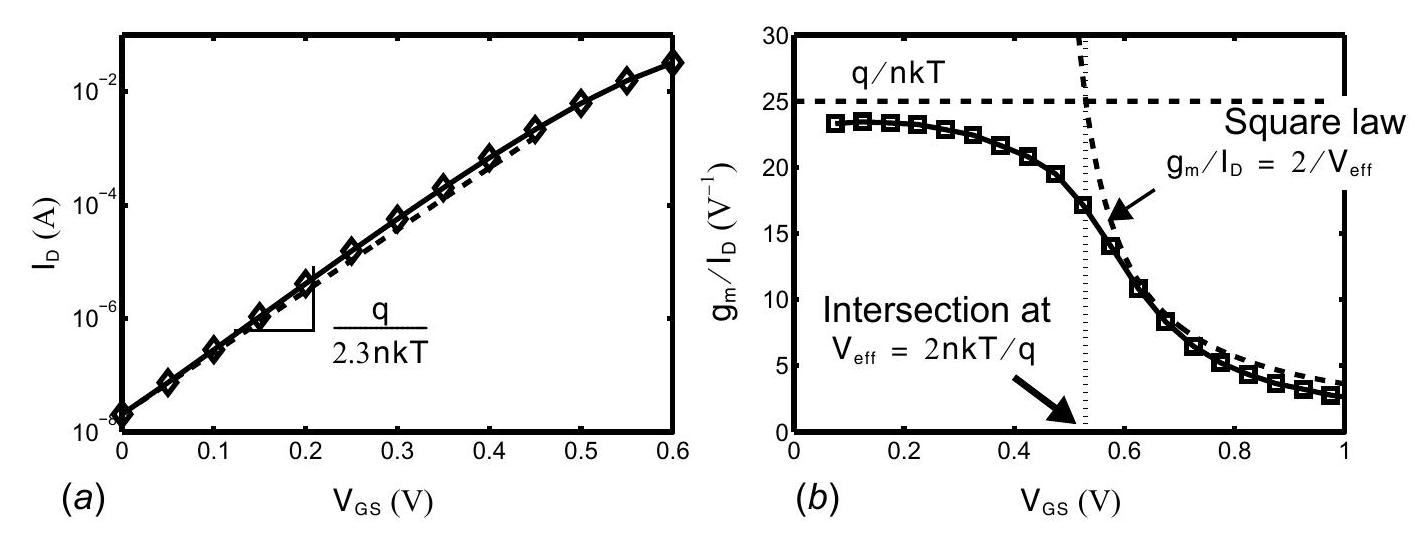
\includegraphics[max width=\textwidth, center]{2024_10_31_60860e27b87166db2267g-068}

Fig. 1.28 Drain current and transconductance of a MOS device in subthreshold.\\
maximum velocity, approximately $10^{7} \mathrm{~cm} / \mathrm{s}$ in silicon. This is referred to as velocity saturation. Vertical electric fields greater than approximately $5 \cdot 10^{6} \mathrm{~V} / \mathrm{m}$ cause the effective channel depth to decrease and also cause more charge-carrier collisions.

For the purposes of design, these effects may be modeled together by an effective carrier mobility that decreases at high $\mathrm{V}_{\text {eff }}$,


\begin{equation*}
\mu_{\mathrm{n}, \mathrm{eff}} \cong \frac{\mu_{\mathrm{n}}}{\left(\left[1+\left(\theta \mathrm{V}_{\mathrm{eff}}\right)^{\mathrm{m}}\right]\right)^{1 / \mathrm{m}}} \tag{1.125}
\end{equation*}


where $\theta$ and $m$ are device parameters. Substituting the effective carrier mobility, $\mu_{n, \text { eff }}$, from (1.125) in place of $\mu_{\mathrm{n}}$ in equation (1.72) gives a new expression for the drain current incorporating mobility degradation.


\begin{equation*}
I_{D}=\frac{1}{2} \mu_{n} C_{o x} \frac{W}{L} V_{\text {eff }}^{2}\left(\frac{1}{\left[1+\left(\theta V_{\text {eff }}\right)^{m}\right]^{1 / m}}\right) \tag{1.126}
\end{equation*}


For small values of $\mathrm{V}_{\text {eft }}$, the final term in equation (1.126) approaches unity and the entire expression simplifies to the square-law relationship in (1.72). For values of $\mathrm{V}_{\text {eff }} \gg 1 / \theta$, the final term in (1.126) approaches $\left(1 / \theta \mathrm{V}_{\text {eff }}\right)$ resulting in a linear relationship between effective gate-source voltage and current. Taking the derivative of (1.126) with respect to gate-source voltage assuming large $\mathrm{V}_{\text {eff }}$ gives a small-signal transconductance that is independent of drain current,


\begin{equation*}
g_{m(\text { mob-deg })}=\frac{1}{2} \mu_{\mathrm{n}} C_{o x} \frac{\mathrm{~W}}{\mathrm{~L}} \frac{1}{\theta} \tag{1.127}
\end{equation*}


Equation (1.127) establishes the maximum transconductance achievable with a given transistor. A square-law model for transconductance (1.73) predicts a transconductance equal to (1.127) when $\mathrm{V}_{\text {eff }}=1 / 2 \theta$. Due to mobility degradation, increases in $\mathrm{V}_{\text {eff }}$ beyond 1/20:

\begin{itemize}
  \item fail to provide significant increases in small-signal transconductance,
  \item reduce the available signal swing limited by the fixed supply voltages, and
  \item reduce transistor intrinsic gain $A_{i}$ dramatically\\
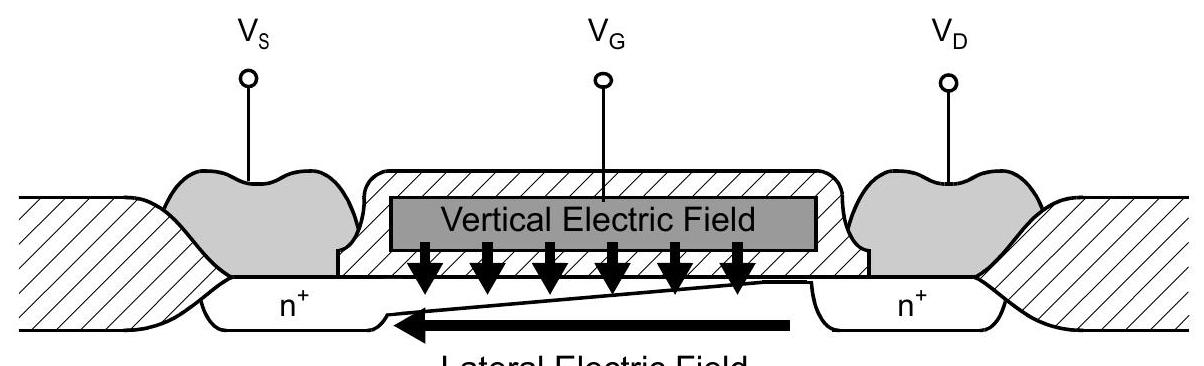
\includegraphics[max width=\textwidth, center]{2024_10_31_60860e27b87166db2267g-069(1)}
\end{itemize}

Lateral Electric Field\\
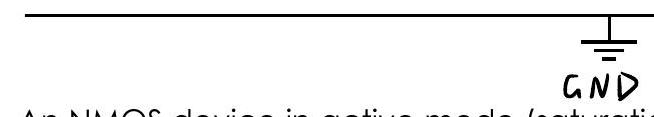
\includegraphics[max width=\textwidth, center]{2024_10_31_60860e27b87166db2267g-069}

Fig. 1.29 An NMOS device in active mode (saturation) identifying the lateral and vertical electric field components.

For these reasons, operation under mobility degradation is generally avoided in analog design, although this is becoming increasingly difficult in modern CMOS processes. Transistors are, however, sometimes biased with $\mathrm{V}_{\text {eff }}>1 / 2 \theta$ when their size must be limited. For example, when very-high frequency operation is sought, parasitic capacitances must be minimized by keeping all transistor dimensions as small as possible.

Key Point: For large values of $\mathrm{V}_{\text {eff }}$, transistors have a sub-square-law voltage current relationship, tending towards a linear relationship for very large values of $\mathrm{V}_{\mathrm{eff}}$

For operating conditions around $\mathrm{V}_{\text {eff }} \approx 1 / 2 \theta$, more sophisticated modeling is required to obtain high accuracy [Sodini, 1984]. However, a piecewise-linear assumption whereby (1.73) is applied when $\mathrm{V}_{\text {eff }}<1 / 2 \theta$ and (1.127) when $\mathrm{V}_{\text {eff }}>1 / 2 \theta$ is often sufficient for first pass design.

In the past, mobility degradation appeared only at extremely large values of $\mathrm{V}_{\text {eff }}$, but this is no longer always the case. Shrinking MOS device dimensions have meant that lower voltages are required to generate the critical electric fields. The value of $\theta$ increases from around $0.06 \mathrm{~V}^{-1}$ for a $0.8-\mu \mathrm{m}$-long transistor in a $0.8-\mu \mathrm{m}$ CMOS process, to greater than $2 \mathrm{~V}^{-1}$ for minimum-sized devices in modern CMOS processes. Hence, mobility degradation can appear at $\mathrm{V}_{\text {eff }}$ values of only a few hundred mV . Since (1.124) places a fundamental lower limit of $\mathrm{V}_{\text {eff }}>100 \mathrm{mV}$ to ensure operation in strong inversion there remains only a narrow range of effective gate-source voltages for which the square-law voltage-current relationship expressed in (1.72) remains valid in nanoscale CMOS devices. In many voltage-to-current conversion circuits that rely on the square-law characteristic, this inaccuracy can be a major source of error. Taking channel lengths larger than the minimum allowed helps to minimize this degradation.

\section*{EXAMPLE 1.18}
Estimate the value of $\theta$ based on the data in Fig. 1.30.

\section*{Solution}
Mobility degradation is evident at high values of $\mathrm{V}_{\text {eff }}$ where the drain current in Fig. 1.30(a) is clearly subquadratic. An estimate of $\theta$ is more easily obtained from the plot of $g_{m}$ versus $V_{G s}$ in Fig. 1.30(b). The value of $\mathrm{V}_{\text {eff }}$ at which the transconductance ceases to follow a linear relationship is approximately $1 / 2 \theta$. In this case, this\\
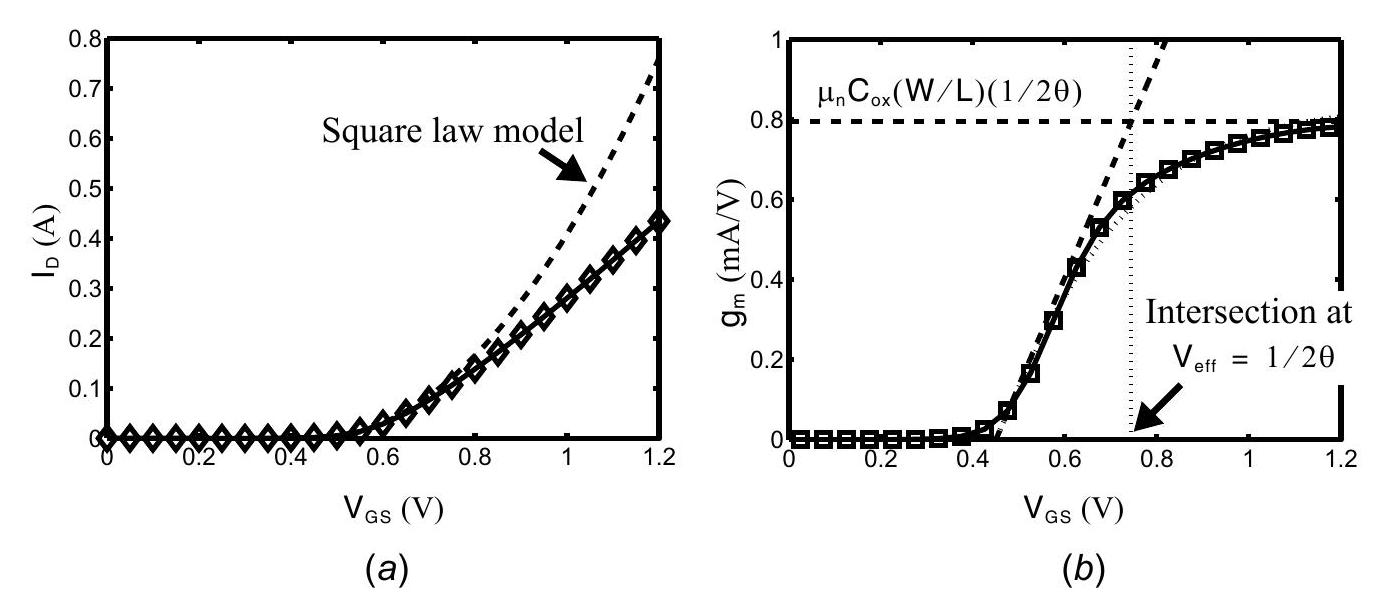
\includegraphics[max width=\textwidth, center]{2024_10_31_60860e27b87166db2267g-070}

Fig. 1.30 Drain current and transconductance of a MOS device in at large values of $\mathrm{V}_{\text {eff }}$.\\
occurs at approximately $\mathrm{V}_{\mathrm{GS}}=0.75 \mathrm{~V}$ or $\mathrm{V}_{\text {eff }}=0.3 \mathrm{~V}$, corresponding to $\theta \cong 1.7 \mathrm{~V}^{-1}$. At $\mathrm{V}_{\text {eff }}>0.3 \mathrm{~V}$, the constant $\mu_{n} C_{o x}(W / L)(1 / 2 \theta) \quad$ can be used as a rough estimate of $g_{m}$. More accuracy is provided using the model of (1.126) with, in this case, a value $\mathrm{m}=1.6$ resulting in the dotted line on Fig. 1.30(b).

\subsection*{1.4.3 Summary of Subthreshold and Mobility Degradation Equations}
The key expressions for operation in subthreshold, stronginversion, and mobility degradation are summarized in Table 1.1 and the progression of transistor drain current and smallsignal transconductance as its gate-source voltage is swept is sketched in Fig. 1.31. Transition regions appear at the borders between these operating modes where the voltage-current relationship and small-signal transconductance are compromises between the expressions in the table. Generally, operation in or near subthreshold is considered only for analog circuits where low-power but low-speed operation is required. Operation under mobility degradation is necessary only when very highspeed is required, thus demanding minimal parasitic capacitances and, hence, low device aspect ratios.

\subsection*{1.4.4 Parasitic Resistances}
Parasitic resistance appears in series with all four MOSFET terminals. The resistance of the polysilicon gate carries no dc current, but may be significant in small-signal analysis since it is in series with the gate-source capacitance, $\mathrm{C}_{\mathrm{gs}}$. Contacts to the drain and source region are resistive and may have significant voltage drops across them when carrying large currents. Additionally, in modern CMOS processes, the drain\\
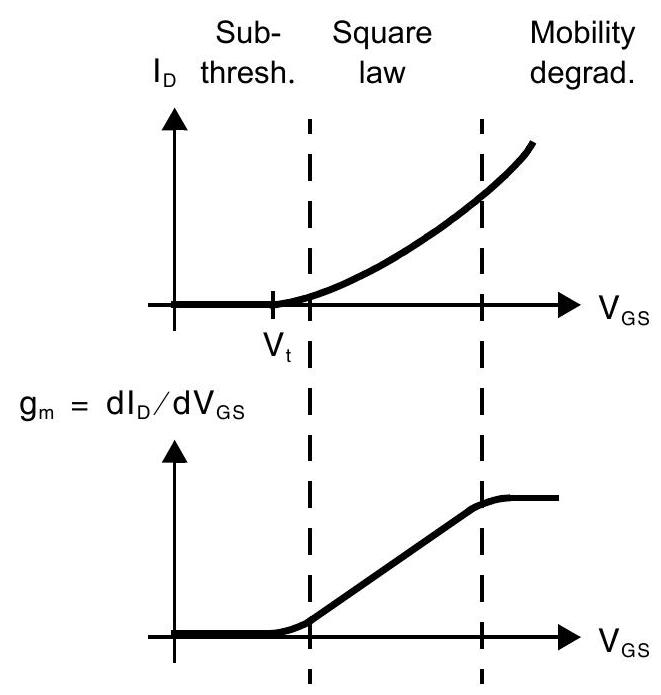
\includegraphics[max width=\textwidth, center]{2024_10_31_60860e27b87166db2267g-071}

Fig. 1.31 The progression of transistor drain current and small-signal transconductance from subthreshold to square law to mobility degradation.

Table 1.1 A summary of MOS device operation in the subthreshold, strong inversion, and mobility degradation regions.

\begin{center}
\begin{tabular}{|c|c|c|c|}
\hline
 & Subthreshold (exponential) & Strong Inversion (square-law) & Mobility Degradation (linear) \\
\hline
Region of validity & $V_{\text {eff }} \lesssim 0$ & \( \frac{2 n k T}{q}<V_{\text {eff }}<\frac{1}{2 \theta} \) & $V_{\text {eff }}>\frac{1}{2 \theta}$ \\
\hline
Drain current, $\mathrm{I}_{\mathrm{D}}$ & $I_{D 0}\left(\frac{W}{L}\right) e^{\left(q V_{\text {eff }} / n \mathrm{TT}\right)}$ & \( \frac{1}{2} \mu_{n} C_{o x} \frac{W}{L} V_{\text {eff }}^{2} \) & \( \frac{0.5 \mu_{n} C_{o x}(W / L) V_{\text {eff }}^{2}}{\left[1+\left(\theta V_{\text {eff }}\right)^{m}\right]^{1 / m}} \) \\
\hline
Small-signal transconductance, $\mathrm{g}_{\mathrm{m}}$ & \( \frac{q l_{D}}{n k T} \) & \( \frac{2 I_{D}}{V_{\text {eff }}}=\mu_{n} C_{o x} \frac{W}{L} V_{\text {eff }} \) & \( \frac{1}{2} \mu_{n} C_{o x} \frac{W}{L} \frac{1}{\theta} \) \\
\hline
Most useful & Very low-power operation & Most analog design & Very high-speed operation \\
\hline
\end{tabular}
\end{center}

and source regions themselves are engineered to have a very shallow depth near the channel region. These shallow source and drain extensions present a narrow cross-sectional area through which all channel current must flow resulting in significant series resistance. Finally, the body terminal is relatively lightly doped semiconductor and, hence, may impose a significant series resistance. All of these parasitics are generally on the order of a few Ohms, and hence are only considered when they are conducting very large currents, or at very high frequencies where the resistances combine with transistor parasitic capacitances to form small-signal poles of significance. Furthermore, they can often be minimized by proper design (for example, by providing additional contacts). They are considered negligible throughout the remainder of the text.

\subsection*{1.4.5 Short-Channel Effects}
A number of short-channel effects degrade the operation of MOS transistors as device dimensions are scaled down. These effects include reduced output impedance and hot-carrier effects (such as oxide trapping and substrate currents). These short-channel effects will be briefly described here. For more detailed modelling of shortchannel effects, see [Wolf, 1995].

Transistors with short channel lengths experience a reduced output impedance because depletion region variations at the drain end (which affect the effective channel length) have an increased proportional effect on the drain current. In addition, a phenomenon known as drain-induced barrier lowering (DIBL) effectively lowers $\mathrm{V}_{\mathrm{t}}$ as $\mathrm{V}_{\mathrm{DS}}$ is increased, thereby further lowering the output impedance of a short-channel device.

Another important short-channel effect is due to hot carriers. These high-velocity carriers can cause harmful effects, such as the generation of electron-hole pairs by impact ionization and avalanching. These extra electronhole pairs can cause currents to flow from the drain to the substrate, as shown in Fig. 1.32. This effect can be modelled by a finite drain-to-ground impedance. As a result, this effect is one of the major limitations on achieving very high output impedances of cascode current sources. In addition, this current flow can cause voltage drops across the substrate and possibly cause latch-up, as the next chapter describes.

Another hot-carrier effect occurs when electrons gain energies high enough to tunnel into and possibly through the thin gate oxide. Thus, this effect can cause dc gate currents. However, often more harmful is the fact that any charge trapped in the oxide will cause a shift in transistor threshold voltage. As a result, hot carriers are one of the major factors limiting the long-term reliability of MOS transistors.\\
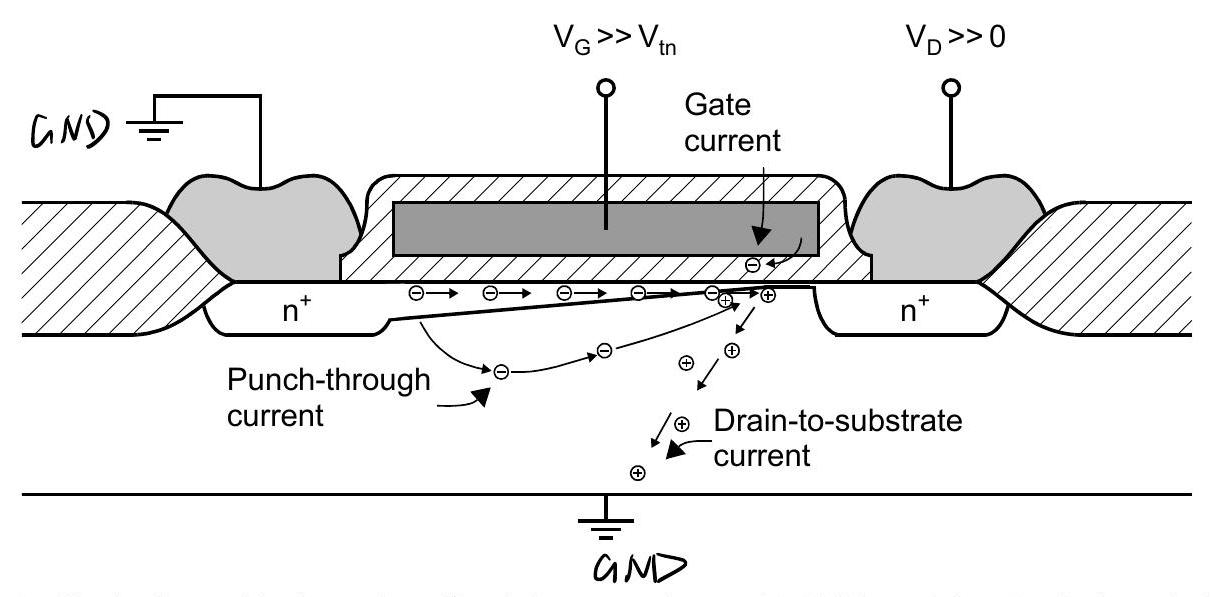
\includegraphics[max width=\textwidth, center]{2024_10_31_60860e27b87166db2267g-072}

Fig. 1.32 An illustration of hot carrier effects in an n-channel MOS transistor. Drain-to-substrate current is caused by electron-hole pairs generated by impact ionization at the drain end of the channel.

A third hot-carrier effect occurs when electrons with enough energy punch through from the source to the drain. As a result, these high-energy electrons are no longer limited by the drift equations governing normal conduction along the channel. This mechanism is somewhat similar to punch-through in a bipolar transistor, where the collector depletion region extends right through the base region to the emitter. In a MOS transistor, the channel length becomes effectively zero, resulting in unlimited current flow (except for the series source and drain impedances, as well as external circuitry). This effect is an additional cause of lower output impedance and possibly transistor breakdown.

All of the hot-carrier effects just described are more pronounced for n -channel transistors than for their p -channel counterparts because electrons have larger velocities than holes.

\subsection*{1.4.6 Leakage Currents}
Leakage currents impose limitations on how long a dynamically charged signal can be maintained in a high impedance state, and on the minimum power consumption achievable when an analog circuit is in an idle (powerdown) state. Three leakage currents are important in MOS transistors: subthreshold leakage, gate leakage, and junction leakage. Of these, subthreshold leakage is often the largest. It results in a finite drain current even when the transistor is off, and was described in detail in section 1.4.1. Gate leakage results from quantum-mechanical tunneling of electrons through very thin gate oxides, and can be significant in digital circuits and when large gate areas are used, for example to implement a capacitor. Finally, the reverse-biased source-body and drain-body pn junctions conduct a finite leakage current. This leakage can be important, for example, in estimating the maximum time a sample-and-hold circuit or a dynamic memory cell can be left in hold mode. The leakage current of a reverse-biased junction (not close to breakdown) is approximately given by\\
where $A_{j}$ is the junction area, $n_{i}$ is the intrinsic concentration of carriers in undoped silicon, $\tau_{0}$ is the effective minority carrier lifetime, $\mathbf{X}_{\mathrm{d}}$ is the thickness of the depletion region, and $\tau_{0}$ is given by


\begin{equation*}
\tau_{0} \cong \frac{1}{2}\left(\tau_{n}+\tau_{p}\right) \tag{1.129}
\end{equation*}


where $\tau_{n}$ and $\tau_{p}$ are the electron and hole lifetimes. Also, $\mathbf{x}_{\mathrm{d}}$ is given by


\begin{equation*}
\mathrm{x}_{\mathrm{d}}=\sqrt{\frac{2 \mathrm{~K}_{\mathrm{s}} \varepsilon_{0}}{\mathrm{qN}}\left(\Phi_{\mathrm{A}}+\mathrm{V}_{\mathrm{r}}\right)} \tag{1.130}
\end{equation*}


and $\mathrm{n}_{\mathrm{i}}$ is given by


\begin{equation*}
\mathrm{n}_{\mathrm{i}} \cong \sqrt{\mathrm{~N}_{\mathrm{C}} \mathrm{~N}_{\mathrm{V}}} \mathrm{e}^{\left(-\mathrm{E}_{\mathrm{g}}\right) /(\mathrm{KT})} \tag{1.131}
\end{equation*}


where $N_{C}$ and $N_{V}$ are the densities of states in the conduction and valence bands and $E_{g}$ is the difference in energy between the two bands.

Since the intrinsic concentration, $\mathrm{n}_{\mathrm{i}}$, is a strong function of temperature (it approximately doubles for every temperature increase of $11^{\circ} \mathrm{C}$ for silicon), the leakage current is also a strong function of temperature. The leakage current roughly doubles for every $11^{\circ} \mathrm{C}$ rise in temperature; thus, at higher temperatures it is much larger than at room temperature.

\subsection*{1.5 SPICE MODELLING PARAMETERS}
This section briefly describes some of the important model parameters for diodes and MOS transistors used during a SPICE simulation. It should be noted here that not all SPICE model parameters are described. However, enough are described to enable the reader to understand the relationship between the relative parameters and the corresponding constants used when doing hand analysis.

\subsection*{1.5.1 Diode Model}
There are a number of important dc parameters. The constant $\mathrm{I}_{\mathrm{S}}$ is specified using either the parameter IS or JS in SPICE. These two parameters are synonyms, and only one should be specified. A typical value specified for $\mathrm{I}_{\mathrm{S}}$ might be between $10^{-18} \mathrm{~A}$ and $10^{-15} \mathrm{~A}$ for small diodes in a microcircuit. Another important parameter is called the emission coefficient, $\mathrm{n}_{\mathrm{j}}$. This constant multiplies $\mathrm{V}_{\mathrm{T}}$ in the exponential diode I-V relationship given by


\begin{equation*}
I_{D}=I_{S} e^{V_{B E} /\left(n_{i} V_{T}\right)} \tag{1.132}
\end{equation*}


The SPICE parameter for $\mathrm{n}_{\mathrm{j}}$ is N and is defaulted to 1 when not specified ( 1 is a reasonable value for junctions in an integrated circuit). A third important dc characteristic is the series resistance, which is specified in SPICE using RS. It should be noted here that some SPICE programs allow the user to specify the area of the diode, whereas others expect absolute parameters that already take into account the effective area. The manual for the program being used should be consulted.

The diode transit time is specified using the SPICE parameter TT. The most important capacitance parameter specified is CJ. CJO and CJ are synonyms - one should never specify both. This parameter specifies the capacitance at $0-\mathrm{V}$ bias. Once again, it may be specified as absolute or as relative to the area (i.e., $\mathrm{F} / \mathrm{m}^{2}$ ), depending on the version of SPICE used. Also, the area junction grading coefficient, MJ, might be specified to determine the exponent used in the capacitance equation. Typical values are 0.5 for abrupt junctions and 0.33 for graded junctions. In some SPICE versions, it might also be possible to specify the sidewall capacitance at 0 -V bias as well as its grading junction coefficient. Finally, the built-in potential of the junction, which is also used in calculating the capacitance, can be specified using PB. PHI, VJ, and PHA are all synonyms of PB.

Reasonably accurate diode simulations can usually be obtained by specifying only IS, CJ, MJ, and PB. However, most modern versions of SPICE have many more parameters that can be specified if one wants accurate temperature and noise simulations. Users should consult their manuals for more information.

Table 1.2 summarizes some of the more important diode parameters. This set of parameters constitutes a minimal set for reasonable simulation accuracy under ordinary conditions.

Table 1.2 Important SPICE parameters for modelling diodes.

\begin{center}
\begin{tabular}{llll}
\hline
\begin{tabular}{l}
SPICE \\
Parameter \\
\end{tabular} & \begin{tabular}{c}
Model \\
Constant \\
\end{tabular} & \multicolumn{1}{c}{Brief Description} & Typical Value \\
\hline
IS & $\mathrm{I}_{\mathrm{S}}$ & Transport saturation current & $10^{-17} \mathrm{~A}$ \\
RS & $\mathrm{R}_{\mathrm{d}}$ & Series resistance & $30 \Omega$ \\
TT & $\tau_{\mathrm{T}}$ & Diode transit time & 12 ps \\
CJ & $\mathrm{C}_{\mathrm{j} 0}$ & Capacitance at 0-V bias & 0.01 pF \\
MJ & $\mathrm{m}_{\mathrm{j}}$ & Diode grading coefficient exponent & 0.5 \\
PB & $\Phi_{0}$ & Built-in diode contact potential & 0.9 V \\
\hline
\end{tabular}
\end{center}

\subsection*{1.5.2 MOS Transistors}
Modern MOS models are quite complicated, so only some of the more important MOS parameters used in SPICE simulations are described here. These parameters are used in what are called the Level 2 or Level 3 models. The model level can be chosen by setting the SPICE parameter LEVEL to either 2 or 3 . The oxide thickness, $\mathrm{t}_{\mathrm{ox}}$, is specified using the SPICE parameter TOX. If it is specified, then it is not necessary to specify the thin gate-oxide capacitance ( $\mathrm{C}_{\mathrm{ox}}$, specified by parameter COX). The mobility, $\mu_{n}$, can be specified using UO. If UO is specified, the intrinsic transistor conductance ( $\mu_{\mathrm{n}} \mathrm{C}_{\mathrm{ox}}$ ) will be calculated automatically, unless this automatic calculation is overridden by specifying either KP (or its synonym, BETA). The transistor threshold voltage at $\mathrm{V}_{\mathrm{S}}=0 \mathrm{~V}, \mathrm{~V}_{\mathrm{tn}}$, is specified by VTO. The body-effect parameter, $\gamma$, can be specified using GAMMA, or it will be automatically calculated if the substrate doping, $\mathrm{N}_{\mathrm{A}}$, is specified using NSUB. Normally, one would not want SPICE to calculate $\gamma$ because the effective substrate doping under the channel can differ significantly from the substrate doping in the bulk due to threshold-voltage adjust implants. The output impedance constant, $\lambda$, can be specified using LAMBDA. Normally, LAMBDA should not be specified since it takes precedence over internal calculations and does not change the output impedance as a function of different transistor lengths or bias voltages (which should be the case). Indeed, modelling the transistor output impedance is one of weakest points in SPICE. If LAMBDA is not specified, it is calculated automatically. The surface inversion potential, $\left|2 \phi_{F}\right|$, can be specified using PHI, or it will be calculated automatically. Another parameter usually specified is the lateral diffusion of the junctions under the gate, $L_{D}$, which is specified by LD. For accurate simulations, one might also specify the resistances in series with the source and drain by specifying RS and RD (typically only the source resistance is important). Many other parameters exist to model such things as short-channel effects, subthreshold effects, and channel-width effects, but these parameters are outside the scope of this book.

The modelling of parasitic capacitances in SPICE is quite involved. The capacitances under the junctions per unit area at $0-\mathrm{V}$ bias, (i.e., $\mathrm{C}_{\mathrm{j} 0}$ ) can be specified using CJ or can be calculated automatically from the specified substrate doping. The sidewall capacitances at $0 \mathrm{~V}, \mathrm{C}_{\mathrm{j} \text {-sw0 }}$, should normally be specified using CJSW because this parameter is used to calculate significant parasitic capacitances. The bulk grading coefficient specified by MJ can usually be defaulted to 0.5 . Similarly, the sidewall grading coefficient specified by MJSW can usually be defaulted to 0.33 (SPICE assumes a graded junction). The built-in bulk-to-junction contact potential, $\Phi_{0}$, can be specified using PB or defaulted to 0.8 V (note that 0.9 V would typically be more accurate, but the resulting simulation differences are small). Sometimes the gate-to-source or drain-overlap capacitances can be specified using CGSO or CGDO, but normally these would be left to be calculated automatically using COX and LD.

Some of the more important parameters that should result in reasonable simulations (except for modelling short-channel effects) are summarized in Table 1.3 for both n - and p -channel transistors. Table 1.3 lists reasonable parameters for a typical $0.8-\mu \mathrm{m}$ technology.

\subsection*{1.5.3 Advanced SPICE Models of MOS Transistors}
Although the SPICE model parameters presented in the last section provide reasonable accuracy for long-channel devices, for channel lengths $L \ll 1 \mu \mathrm{~m}$ their accuracy becomes very poor. Many SPICE MOS models have therefore been developed to try to capture higher-order effects. A summary of the capabilities of the more common modern SPICE model formats is provided in Table 1.4.

Unfortunately, these SPICE models require over 100 parameters to accurately capture transistor operation in all of its modes over a wide range of temperatures. Many parameters are required because, for very small device sizes, fundamental constants such as threshold voltage and effective carrier mobility become dependent on the transistor's exact width and length. Hence, it is strongly recommended that analog designers use only a small set of "unit-sized" transistors, forming all transistors from parallel combinations of these elementary devices.

Table 1.3 A reasonable set of Level 2 or 3 MOS parameters for a typical 0.8- $\mu \mathrm{m}$ technology.

\begin{center}
\begin{tabular}{|c|c|c|c|}
\hline
\begin{tabular}{l}
SPICE \\
Parameter \\
\end{tabular} & \begin{tabular}{l}
Model \\
Constant \\
\end{tabular} & Brief Description & Typical Value \\
\hline
VTO & $\mathrm{V}_{\mathrm{t} \mathrm{n}}: \mathrm{V}_{\mathrm{tp}}$ & Transistor threshold voltage (in V) & 0.8:-0.9 \\
\hline
UO & $\mu_{\mathrm{n}}: \mu_{\mathrm{p}}$ & Carrier mobility in bulk (in $\mathrm{cm}^{2} / \mathrm{V} \cdot \mathrm{s}$ ) & 500:175 \\
\hline
TOX & $t_{\text {ox }}$ & Thickness of gate oxide (in m) & $1.8 \times 10^{-8}$ \\
\hline
LD & $\mathrm{L}_{\mathrm{D}}$ & Lateral diffusion of junction under gate (in m) & $6 \times 10^{-8}$ \\
\hline
GAMMA & $\gamma$ & Body-effect parameter & 0.5: 0.8 \\
\hline
NSUB & $\mathrm{N}_{\mathrm{A}}: \mathrm{N}_{\mathrm{D}}$ & The substrate doping (in $\mathrm{cm}^{-3}$ ) & $3 \times 10^{16}: 7.5 \times 10^{16}$ \\
\hline
PHI & |2 $\phi_{\mathrm{F}} \mid$ & Surface inversion potential (in V) & 0.7 \\
\hline
PB & $\Phi_{0}$ & Built-in contact potential of junction to bulk (in V) & 0.9 \\
\hline
CJ & $\mathrm{C}_{\mathrm{j} 0}$ & Junction-depletion capacitance at $0-\mathrm{V}$ bias (in $\mathrm{F} / \mathrm{m}^{2}$ ) & $2.5 \times 10^{-4}: 4.0 \times 10^{-4}$ \\
\hline
CJSW & $\mathrm{C}_{\mathrm{j} \text {-sw0 }}$ & Sidewall capacitance at $0-\mathrm{V}$ bias (in $\mathrm{F} / \mathrm{m}$ ) & $2.0 \times 10^{-10}: 2.8 \times 10^{-10}$ \\
\hline
MJ & $\mathrm{m}_{\mathrm{j}}$ & Bulk-to-junction exponent (grading coefficient) & 0.5 \\
\hline
MJSW & $\mathrm{m}_{\mathrm{j} \text { sw }}$ & Sidewall-to-junction exponent (grading coefficient) & 0.3 \\
\hline
\end{tabular}
\end{center}

Table 1.4 A summary of modern SPICE model formats.

\begin{center}
\begin{tabular}{ll}
\hline
\begin{tabular}{l}
SPICE \\
Model \\
\end{tabular} & \multicolumn{1}{c}{Main strengths compared with previous device models} \\
\hline
BSIM3 & \begin{tabular}{c}
Improved modeling of moderate inversion, and the geometry-dependence of device \\
parameters. This also marked a return to a more physics-based model as opposed to the \\
preceding highly empirical models. \\
\end{tabular} \\
EKV & \begin{tabular}{l}
Relates terminal currents and voltages with unified equations that cover all modes of transistor \\
operation, hence avoiding discontinuities at transitions between, for example, weak and strong \\
inversion. Also handles geometry-dependent device parameters. \\
\end{tabular} \\
BSIM4 $\quad$\begin{tabular}{l}
Improved modeling of leakage currents and short-channel effects, noise, and parasitic resistance \\
in the MOSFET terminals, as well as continued improvements in capturing the geometry- \\
dependence of device parameters. \\
\end{tabular} &  \\
PSP $\quad$\begin{tabular}{l}
Improved modeling of noise and the many short-channel and layout-dependent effects now \\
dominant in nanoscale CMOS devices. Particular effort was made to accurately model \\
nonlinearities, which requires accuracy in the high-order derivatives of the transistor's \\
voltage-current relationships. \\
\end{tabular} &  \\
\hline
\end{tabular}
\end{center}

For example, for a minimum gate-length of $L_{\text {min }}$, device sizes with $(W / L)=\left(8 L_{\text {min }} / L_{\text {min }}\right),\left(12 L_{\text {min }} / 1.5 L_{\text {min }}\right)$, $\left(16 \mathrm{~L}_{\min } / 2 \mathrm{~L}_{\text {min }}\right)$, and $\left(32 \mathrm{~L}_{\min } / 4 \mathrm{~L}_{\text {min }}\right)$ in both NMOS and PMOS varieties might be chosen. Then, if a transistor of size $(W / L)=\left(240 \mathrm{~L}_{\text {min }} / 2 \mathrm{~L}_{\text {min }}\right)$ is desired, simply combine 15 of the $\left(16 \mathrm{~L}_{\text {min }} / 2 \mathrm{~L}_{\text {min }}\right)$-devices in parallel as shown in Fig. 1.33. Of course this practice restricts the device sizes available for design, but the benefits of having device parameters that are consistent and well-understood far outweigh this minor drawback.

For each device in the set, rough estimates of a few basic model parameters such as $\mu_{n} \mathrm{C}_{\mathrm{ox}}, \mathrm{V}_{\mathrm{tn}}$, etc. may be obtained from simulation data, or better yet measurements, of the unit-sized devices following the procedures in Examples $1.9,1.11,1.17$, and 1.18 . These rough model parameters may be used for the many quick handcalculations performed in the course of first-pass design. Similarly, the unit-transistor's parasitic capacitances may\\
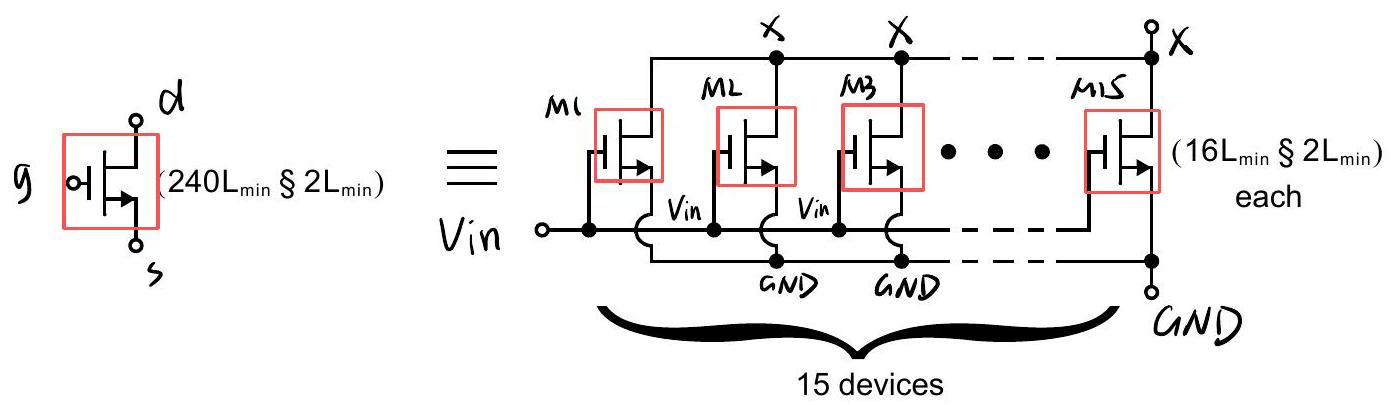
\includegraphics[max width=\textwidth, center]{2024_10_31_60860e27b87166db2267g-077(1)}

Fig. 1.33 Realization of a transistor by parallel combination of small unit-sized transistor elements.\\
be observed under a typical biasing condition; these capacitance values can then be used to obtain rough estimates of circuit parasitics. Several sets of such parameters that are representative of various CMOS technologies are presented in Table 1.5. When refinement and detailed verification of a design are required, these are of course performed with the aid of SPICE and the complete device models.

Some designers prefer to forgo the extraction of device parameters from data and simply refer to plots of device data throughout the design process, looking up small-signal parameters at different operating points. In any case, performing basic device simulations at the outset of any analog design is useful, not only for extracting approximate device parameters from complex MOS models, but also because it may expose shortcomings in the device models themselves or even the simulation environment. For example, discontinuities observed in plots of drain current or its\\
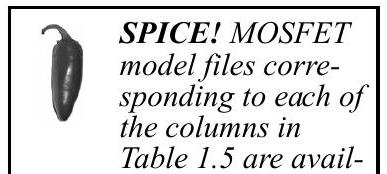
\includegraphics[max width=\textwidth, center]{2024_10_31_60860e27b87166db2267g-077}\\
able on the book web site for simulation exercises.\\
derivatives are an indication that the model may be unreliable in that region.

Table 1.5 MOSFET parameters repre sentative of v arious CMOS technologies and used for rough hand calculations in this text.

\begin{center}
\begin{tabular}{lllllllll}
\hline
 & \multicolumn{2}{c}{$\mathbf{0 . 8} \mu \mathbf{m}$} & \multicolumn{2}{c}{$\mathbf{0 . 3 5} \boldsymbol{\mu m}$} & \multicolumn{2}{c}{$\mathbf{0 . 1 8} \boldsymbol{\mu m}$} & \multicolumn{2}{c}{$\mathbf{4 5} \mathbf{~ n m}$} \\
Technology & NMOS & PMOS & NMOS & PMOS & NMOS & PMOS & NMOS & PMOS \\
\hline
$\mu \mathrm{C}_{\mathrm{ox}}\left(\mu \mathrm{A} / \mathrm{V}^{2}\right)$ & 92 & 30 & 190 & 55 & 270 & 70 & 280 & 70 \\
$\mathrm{~V}_{\mathrm{t} 0}(\mathrm{~V})$ & 0.80 & -0.90 & 0.57 & -0.71 & 0.45 & -0.45 & 0.45 & -0.45 \\
$\lambda \cdot \mathrm{~L}(\mu \mathrm{~m} / \mathrm{V})$ & 0.12 & 0.08 & 0.16 & 0.16 & 0.08 & 0.08 & 0.10 & 0.15 \\
$\mathrm{C}_{\mathrm{ox}}\left(\mathrm{fF} / \mu \mathrm{m}^{2}\right)$ & 1.8 & 1.8 & 4.5 & 4.5 & 8.5 & 8.5 & 25 & 25 \\
$\mathrm{t}_{\mathrm{ox}}(\mathrm{nm})$ & 18 & 18 & 8 & 8 & 5 & 5 & 1.2 & 1.2 \\
n & 1.5 & 1.5 & 1.8 & 1.7 & 1.6 & 1.7 & 1.85 & 1.85 \\
$\theta(1 / \mathrm{V})$ & 0.06 & 0.135 & 1.5 & 1.0 & 1.7 & 1.0 & 2.3 & 2.0 \\
m & 1.0 & 1.0 & 1.8 & 1.8 & 1.6 & 2.4 & 3.0 & 3.0 \\
$\mathrm{C}_{\mathrm{ov}} / \mathrm{W}=\mathrm{L}_{\mathrm{ov}} \mathrm{C}_{\mathrm{ox}}$ & 0.20 & 0.20 & 0.20 & 0.20 & 0.35 & 0.35 & 0.50 & 0.50 \\
$\quad(\mathrm{fF} / \mu \mathrm{m})$ &  &  &  &  &  &  &  &  \\
$\mathrm{C}_{\mathrm{do}} / \mathrm{W} \approx \mathrm{C}_{\mathrm{sb}} / \mathrm{W}$ & 0.50 & 0.80 & 0.75 & 1.10 & 0.50 & 0.55 & 0.45 & 0.50 \\
$(\mathrm{fF} / \mu \mathrm{m})$ &  &  &  &  &  &  &  &  \\
\hline
\end{tabular}
\end{center}

\subsection*{1.6 PASSIVE DEVICES}
Passive components are often required for analog design. However, since transistor performance is the primary consideration in the development of most integrated-circuit fabrication technologies, integrated-circuit passive components exhibit significant nonidealities that must be understood by the analog designer. The most common passive components in analog integrated-circuit design are resistors and capacitors.

\subsection*{1.6.1 Resistors}
\section*{Strip Resistors}
The simplest realization of an integrated-circuit resistor is nothing more than a strip of conductive material above the silicon substrate, as shown in Fig. 1.34. The conductivity of the material from which the strip is made is generally characterized by its sheet resistance, $\mathrm{R}_{\square}$, which is derived in terms of basic material properties in Section 1.7.4 and has units of $\Omega$. This, along with the dimensions of the strip, determine the value of the resistor.


\begin{equation*}
R=R_{\square}\left(\frac{L}{W}\right) \tag{1.133}
\end{equation*}


This equation is also useful for calculating the resistance of interconnects used in integrated circuits. Multiple strips may be combined in series or in parallel to realize the desired total resistance without requiring impractically large or small values of $L$ or $W$.

Strip resistors inevitably have parasitic capacitances to the silicon substrate which is generally held at a constant reference potential. A simple small-signal model is shown in Fig. 1.34. Although strictly speaking the capacitance is distributed evenly along the resistor, this first-order model simply splits the total capacitance into two lumped capacitors at either end of the resistor.

\section*{EXAMPLE 1.19}
In many CMOS manufacturing processes, polysilicon strips are used to provide a controllable sheet resistance for analog design. A typical value is $\mathrm{R}_{\square}=500 \Omega$. If each strip is $1 \mu \mathrm{~m}$ wide and $5 \mu \mathrm{~m}$ long, how many must be connected in series to make a resistor of value $50 \mathrm{k} \Omega$ ?

\section*{Solution}
Each strip has a resistance of

$$
\mathrm{R}=\mathrm{R}_{\square}\left(\frac{\mathrm{L}}{\mathrm{~W}}\right)=500 \Omega\left(\frac{5 \mu \mathrm{~m}}{1 \mu \mathrm{~m}}\right)=2.5 \mathrm{k} \Omega
$$

Hence, 20 must be connected in series to realize the desired total resistance,

$$
\mathrm{R}_{\mathrm{tot}}=20 \mathrm{R}=20(2.5 \mathrm{k} \Omega)=50 \mathrm{k} \Omega
$$

\section*{Semiconductor Resistors}
Integrated-circuit manufacturing processes that are developed primarily for digital design may not include any materials with sufficient sheet resistance to realize practically useful resistor values. In these processes, a lightlydoped section of the silicon substrate with contacts at either end may be used as a resistor. The common case of a\\
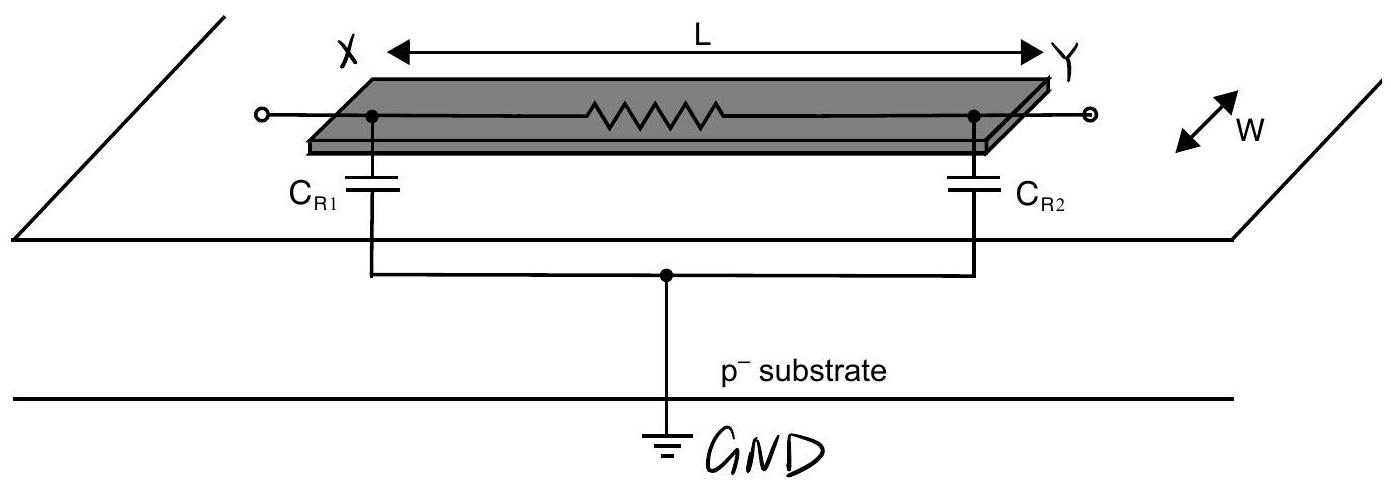
\includegraphics[max width=\textwidth, center]{2024_10_31_60860e27b87166db2267g-079}

Fig. 1.34 A strip-resistor and its model including parasitic capacitances to the grounded substrate.\\
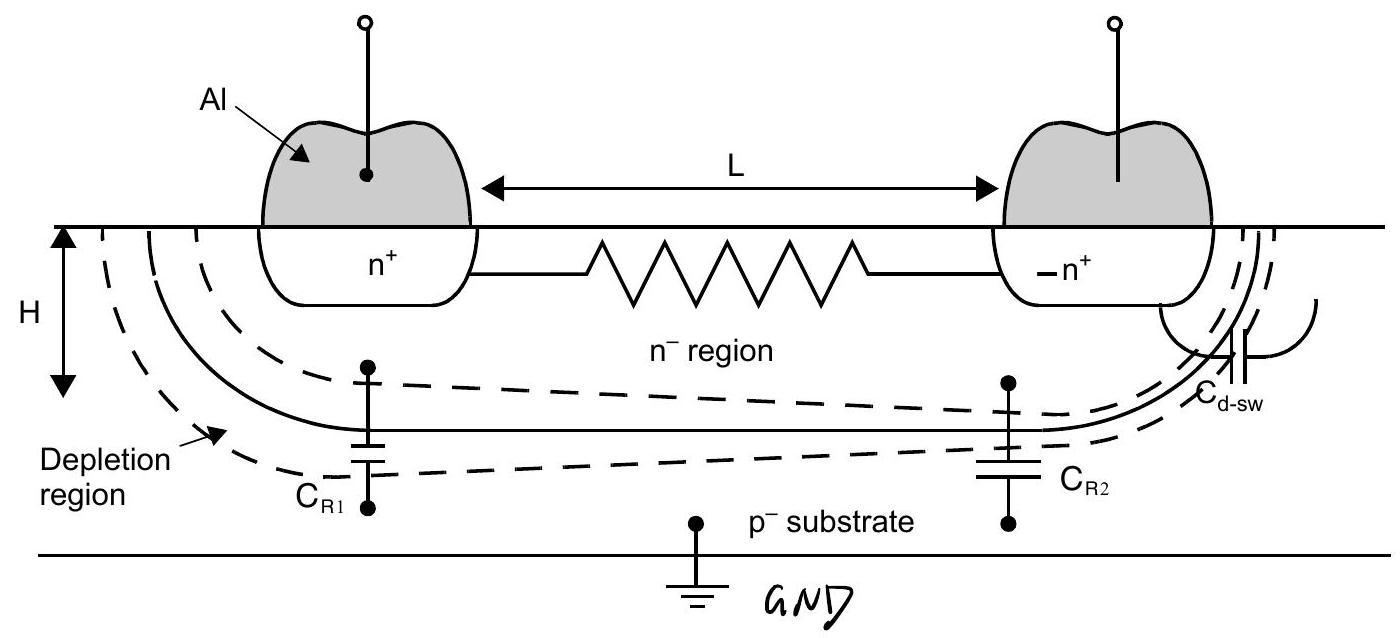
\includegraphics[max width=\textwidth, center]{2024_10_31_60860e27b87166db2267g-079(1)}

Fig. 1.35 A resistor made from a lightly doped semiconductor region with depletion region capacitances shown.\\
type-n resistor in a p-substrate is shown in Fig. 1.35. The resistor is isolated from the grounded substrate by a reverse-biased pn-junction. Depending on the dopant concentration, the effective sheet resistance may be in the range of 10 's of Ohms with a complex temperature dependence. A detailed derivation is presented in section 1.7.4 resulting the in the following sheet resistance, assuming a uniform height (depth) resistor, H :


\begin{equation*}
\mathrm{R}_{\square}=\frac{1}{\mathrm{q} \mu_{\mathrm{n}} \mathrm{Hn} \mathrm{n}_{\mathrm{n}}} \tag{1.134}
\end{equation*}


The small-signal model in Fig. 1.34 is also applicable to semiconductor resistors. However, unlike strip resistors, the parasitic capacitors are junction capacitances so their values depend on the voltages at either end of the resistor. Furthermore, the extent to which the depletion region extends into the resistor also depends upon the resistor's terminal voltages, so its effective cross-section and resistance will change with voltage. This can be problematic for analog design since capacitors and resistors whose values depend on their terminal voltages are nonlinear circuit elements and will introduce harmonic distortion when subjected\\
to time-varying signals. Finally, the parasitic capacitances $C_{R 1}$ and $C_{R 2}$ for semiconductor resistors are typically larger than for strip resistors because they can be located further from the grounded substrate, and because the relative permittivity of silicon $\left(\mathrm{K}_{\mathrm{s}} \cong 11.8\right.$ ) is higher than that of the silicon dioxide insulation above the substrate ( $\mathrm{K}_{\mathrm{ox}} \cong 3.9$ ).

\section*{EXAMPLE 1.20}
A $4 \mathrm{k} \Omega$ resistor is to be formed from a single 3- $\mu \mathrm{m}$-wide strip of type-n silicon with a dopant concentration of $\mathrm{N}_{\mathrm{D}}=10^{23}$ atoms $/ \mathrm{m}^{3}$ that extends to a depth of $\mathrm{H}=2 \mu \mathrm{~m}$ into a type-p substrate that has a dopant concentration of $N_{A}=10^{22}$ atoms $/ \mathrm{m}^{3}$. Find the length of the resistor and estimate the parasitic capacitances. Assume that the resistor-substrate junction has a 3-V reverse bias, and $\mu_{\mathrm{n}}=8 \cdot 10^{-2} \mathrm{~m}^{2} / \mathrm{V} \cdot \mathrm{s}$ inside the resistor.

\section*{Solution}
Substitution into (1.134) yields a sheet resistance of

$$
\mathrm{R}_{\square}=\frac{1}{\left(1.6 \cdot 10^{-19}\right)\left(8 \cdot 10^{-2}\right)\left(2 \cdot 10^{-6}\right)\left(10^{23}\right)}=390 \Omega / \mathrm{sq}
$$

Rearranging (1.133),

$$
\mathrm{L}=\left(\frac{\mathrm{R}}{\mathrm{R}_{\square}}\right) \mathrm{W}=\left(\frac{4 \mathrm{k} \Omega}{0.39 \mathrm{k} \Omega}\right) 3 \mu \mathrm{~m}=31 \mu \mathrm{~m}
$$

This lightly-doped junction has a built-in voltage lower than was calculated in Example 1.2.

$$
\Phi_{0}=0.026 \times \ln \left(\frac{10^{23} \times 10^{22}}{\left(1.1 \times 10^{16}\right)^{2}}\right)=0.77 \mathrm{~V}
$$

The junction capacitance per unit area, assuming an abrupt one-sided junction $\left(N_{A}\right.$ « $\left.N_{D}\right)$ and using the reverse bias voltage $\mathrm{V}_{\mathrm{R}}=3 \mathrm{~V}$, may be calculated as follows:

$$
\begin{gathered}
\mathrm{C}_{\mathrm{j} 0}=\sqrt{\frac{\mathrm{qK}_{\mathrm{s}} \varepsilon_{0} \mathrm{~N}_{\mathrm{A}}}{2 \Phi_{0}}}=\sqrt{\frac{1.6 \times 10^{-19} \times 11.8 \times 8.854 \times 10^{-12} \times 10^{22}}{2 \times 0.77}}=0.33 \mathrm{fF} / \mu \mathrm{m}^{2} \\
\mathrm{C}_{\mathrm{j}}=\frac{\mathrm{C}_{\mathrm{j} 0}}{\sqrt{1+\frac{\mathrm{V}_{\mathrm{B}}}{\Phi_{0}}}}=\frac{0.33}{\sqrt{1+\frac{3}{0.77}}} \mathrm{fF} / \mu \mathrm{m}^{2}=0.15 \mathrm{fF} / \mu \mathrm{m}^{2}
\end{gathered}
$$

The resistor forms a pn-junction with an area of $\mathrm{WL}=(3 \mu \mathrm{~m} \cdot 31 \mu \mathrm{~m})=93 \mu \mathrm{~m}^{2}$ and sidewalls having an area approximately equal to the resistor perimeter times its height,

$$
A_{s w}=(3 \mu \mathrm{~m}+31 \mu \mathrm{~m}+3 \mu \mathrm{~m}+31 \mu \mathrm{~m}) \cdot 2 \mu \mathrm{~m}=136 \mu \mathrm{~m}^{2}
$$

Adopting the simple model of Fig. 1.35 and assuming negligible voltage drop across the resistor, the total capacitance may be divided equally between the two resistor terminals.

$$
C_{R 1}=C_{R 2}=\frac{\left(W L+A_{s w}\right) C_{i}}{2}=\frac{(93+136) 0.15}{2} \mathrm{fF}=17 \mathrm{fF}
$$

\section*{Triode MOS Resistors}
There is a third method to realize resistors on an integrated circuit with which the reader is already familiar: a MOS device in triode. Pictured in Fig. 1.11, this is effectively a semiconductor resistor where the channel depth, and hence resistance, are modulated by a gate voltage. Therefore, like semiconductor resistors, triode MOS devices exhibit nonlinear resistance and parasitic capacitances. But, because the conducting channel region is much shallower than in semiconductor resistors, the resistance is even more nonlinear than a semiconductor resistor. Typically, MOS triode resistors are only used when the voltage across the resistor terminals (i.e. the drain and source of the MOS device) will remain significantly less than $\mathrm{V}_{\text {eff }}$.

In spite of these shortcomings, MOS devices in triode have two unique properties that make them very useful as resistors in analog integrated-circuit design. First, the value of resistance may be tuned via a third terminal: the gate voltage. Second, relatively large values of resistance can be realized in a very compact area.

\section*{EXAMPLE 1.21}
As in Example 1.19, you require a resistor of value $50 \mathrm{k} \Omega$. However, since the voltage across the resistor is never expected to exceed 200 mV , you decide it is feasible to use a n-channel MOS devices in triode to implement it. You elect to use multiple devices sized $\mathrm{W} / \mathrm{L}=2 \mu \mathrm{~m} / 1 \mu \mathrm{~m}$ to avoid short-channel effects. If $\mu_{\mathrm{n}} \mathrm{C}_{\mathrm{ox}}=300 \mu \mathrm{~A} / \mathrm{V}^{2}$, $\mathrm{V}_{\mathrm{tn}}=0.3 \mathrm{~V}$, and you elect to use $\mathrm{V}_{\mathrm{GS}}=1 \mathrm{~V}$, find the number of series devices required to implement the resistor. Compare the resulting device area to that calculated in Example 1.19 for a strip resistor.

\section*{Solution}
The resistance of a device in triode is given in equation (1.104).

$$
\begin{aligned}
r_{\mathrm{ds}} & =\left(\mu_{\mathrm{n}} C_{\mathrm{ox}}\left(\frac{\mathrm{~W}}{\mathrm{~L}}\right)\left(\mathrm{V}_{\mathrm{GS}}-\mathrm{V}_{\mathrm{tn}}\right)\right)^{-1} \\
& =\left(300 \mu \mathrm{~A} / \mathrm{V}^{2}\left(\frac{2 \mu \mathrm{~m}}{1 \mu \mathrm{~m}}\right)(1 \mathrm{~V}-0.3 \mathrm{~V})\right)^{-1} \\
& =2.38 \mathrm{k} \Omega
\end{aligned}
$$

With 21 such devices in series, the desired resistance $21 \cdot 2.38 \mathrm{k} \Omega=50 \mathrm{k} \Omega$ is realized. This is considerably smaller than combining 20 strip resistors in series, each $5 \mu \mathrm{~m} \times 1 \mu \mathrm{~m}$, as in Example 1.19.

Regardless of how they are implemented, resistor values vary greatly from one integrated circuit to another and with changes in temperature. Fortunately, with some care it is possible to ensure that such variations effect all\\
resistors on a given integrated circuit approximately equally. Analog integrated circuits must often be designed to function properly even when the resistor values change by $10-40 \%$.

\subsection*{1.6.2 Capacitors}
\section*{pn Junction Capacitors}
The capacitance provided by reverse-biased pn-junctions has already been discussed in Section 1.1. Junction capacitances may be introduced intentionally into an analog design to serve as a capacitor. They provide a relatively high value of capacitance per unit area since the depletion region can be quite thin and the relative permittivity of silicon is quite high ( $\mathrm{K}_{\mathrm{s}} \cong 11.8$ ). Their capacitance can be tuned by adjusting the voltage across them. When used to realize a variable capacitor in this way, they are called varactors.

Unfortunately, several features of junction capacitances pose problems for analog design. First, although the tunability of their capacitance is useful in some applications, it also makes them nonlinear elements that distort time-varying signals. Second, the value of capacitance realized by a given size junction varies considerably with dopant concentration which is difficult to control during integrated circuit manufacturing. Finally, junction capacitors have more leakage current than other types of integrated circuit capacitors. The most common application for pn junction capacitors is as a varactor in tunable radio-frequency circuits, notably oscillators, although even there MOS capacitors are now often favoured.

\section*{MOS Capacitors}
Since the gate oxide is the thinnest dielectric available in an integrated circuit, it is imminently sensible to build capacitors around it. There are many ways to do so. All comprise gate and silicon conducting "plates" separated by the gate oxide as a dielectric. All are nonlinear capacitors, whose value depends on the voltage across it. The detailed modeling of all of these is beyond the scope of this section, so we will focus on just one common structure: the PMOS transistor.

When using a PMOS transistor, one terminal is the gate and the other is the source, drain, and body all shorted together underneath, shown schematically in Fig. 1.36(a). In this configuration, $\mathrm{V}_{\mathrm{DS}}=0$ and $\mathrm{V}_{\mathrm{SG}}=-\mathrm{V}_{\mathrm{GS}}$ is the voltage on the capacitor. Small-signal models for a NMOS transistor in this mode were covered in Section 1.2.8, but the salient points are repeated here for a PMOS device.

If $\mathrm{V}_{\mathrm{SG}}>\left|\mathrm{V}_{\mathrm{tp}}\right|$, the device enters triode and the small-signal capacitance is given by the sum of $\mathrm{C}_{\mathrm{gs}}$ and $\mathrm{C}_{\mathrm{gd}}$ from equation (1.105) and two overlap capacitances, $\mathrm{C}_{\mathrm{ov}}$, from equation (1.90).


\begin{equation*}
\mathrm{C}_{\text {Mos(on) }}=\mathrm{WLC}_{\mathrm{ox}}+2 \mathrm{WL}_{\mathrm{ov}} \mathrm{C}_{\mathrm{ox}} \tag{1.135}
\end{equation*}


\begin{center}
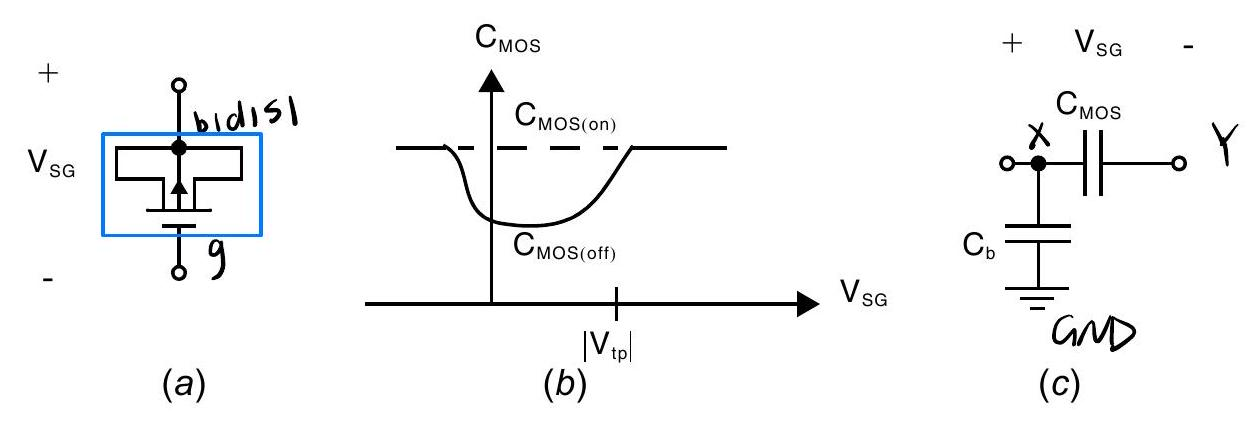
\includegraphics[max width=\textwidth]{2024_10_31_60860e27b87166db2267g-082}
\end{center}

Fig. 1.36 A PMOS capacitor: (a) schematic symbol; (b) nonlinear capacitance; (c) small-signal model.

If $\mathrm{V}_{\mathrm{SG}}<\left|\mathrm{V}_{\mathrm{tp}}\right|$, the channel under the device turns off and the small-signal capacitance is mainly provided by only the overlap capacitances $\mathrm{C}_{\mathrm{gs}}$ and $\mathrm{C}_{\mathrm{gd}}$ in equation (1.110).


\begin{equation*}
\mathrm{C}_{\text {MOS(off) }} \cong 2 \mathrm{WL}_{\mathrm{ov}} \mathrm{C}_{\mathrm{ox}} \tag{1.136}
\end{equation*}


Here, we have neglected $\mathrm{C}_{g b}$ which is assumed to be much smaller. Finally, if $\mathrm{V}_{\mathrm{SG}}$ becomes significantly less than zero, the silicon immediately under the gate will eventually accumulate n-type carriers and become conducting again, thus increasing the small-signal capacitance back to a value close to (1.135). Hence, the structure's smallssignal capacitance varies with voltage as shown in Fig. 1.36(b).

The PMOS body terminal is typically a $n$-type well in the p -type substrate, isolated from ground by a reversebiased pn-junction. This of course introduces a junction capacitance between the body and ground, $\mathrm{C}_{\mathrm{b}}$, which can be quite large and whose value varies with changes in the body voltage. A simple small-signal model is shown in Fig. 1.36(c). For more accurate modeling, a series resistance may be included in series with $\mathrm{C}_{\text {mos }}$ due to the resistance of the inverted channel or body region.

Clearly this is a highly nonlinear capacitor and should be used with care in analog design. Nevertheless, it is popular for three reasons. First, because it is relatively well-modeled by standard circuit simulators. It is, after all, a transistor. Second, the very thin gate oxide ensures a high capacitance-per-unit-area. Third, it requires no special modifications to CMOS integrated-circuit fabrication processes.

\section*{Metal-metal}
To realize a purely linear capacitance on an integrated circuit, it is necessary to avoid the use of semiconductors for either plate. Instead, the many electrically-isolated layers of conductors above the silicon substrate are used.

Two different geometries used to implement metal-metal capacitors are shown in Fig. 1.37. The capacitance of the parallel-plate structure is approximately


\begin{equation*}
\mathrm{C} \cong \frac{\varepsilon_{\mathrm{ox}} \mathrm{~A}}{\mathrm{t}_{\mathrm{ox}}} \tag{1.137}
\end{equation*}


where $t_{\mathrm{ox}}$ is the spacing between plates (on the order of $0.1-10 \mu \mathrm{~m}$ ), $\varepsilon_{\mathrm{ox}}$ is the permittivity of the insulator between plates (often silicon dioxide, for which $\varepsilon_{0 x} \cong 3.9 \varepsilon_{0}$ ), and A is the area of the plate. Equation (1.137) neglects the fringe fields around the edges of the capacitor, but these are relatively small if the capacitor area is large. Some integrated circuits are specially engineered to provide parallel-plate capacitors with very small $t_{0 x}$ and/or large $\varepsilon_{0 x}$, thus permitting small area A for a given value of capacitance. For example, two polysilicon (gate) layers are sometimes stacked on top of each other very closely to realize a "double-poly capacitor". ${ }^{16}$ If no such provision is made, the normal metal layers intended for wiring may be used.

The parallel-plate structure is asymmetric since the bottom plate is in closer proximity to the silicon substrate and electrically shields the top plate from ground. Hence, the bottom plate has a larger parasitic capacitance, $\mathrm{C}_{p 1}$ » $\mathrm{C}_{p 2}$. This can often be exploited in analog designs by connecting the bottom plate to a node with a constant potential with respect to ground, thus minimizing parasitics on the plate with time-varying potential. In light of this, a slightly different symbol is used in this book, as shown in Fig. 1.37(a), when the distinction between top and bottom plate is crucial.

The side-wall capacitive structure shown in Fig. 1.37(b) is becoming increasingly popular in modern integrated circuits where metal wires may actually be made thinner (when viewed from above) than their height. Hence, routing many of them immediately next to each other can provide a large total capacitance. In fact, the capacitance-per-unit-area of such a structure is often greater than parallel-plate metal-metal structures (unless special high-density parallel-plate capacitors are available). The structure is symmetric, with equal parasitics on either side of the capacitor, $\mathrm{C}_{\mathrm{p} 1}=\mathrm{C}_{\mathrm{p} 2}$. However, the capacitance is more difficult to estimate since it is largely provided by fringing electrical fields so appropriate computer tools are required to properly design them.\\
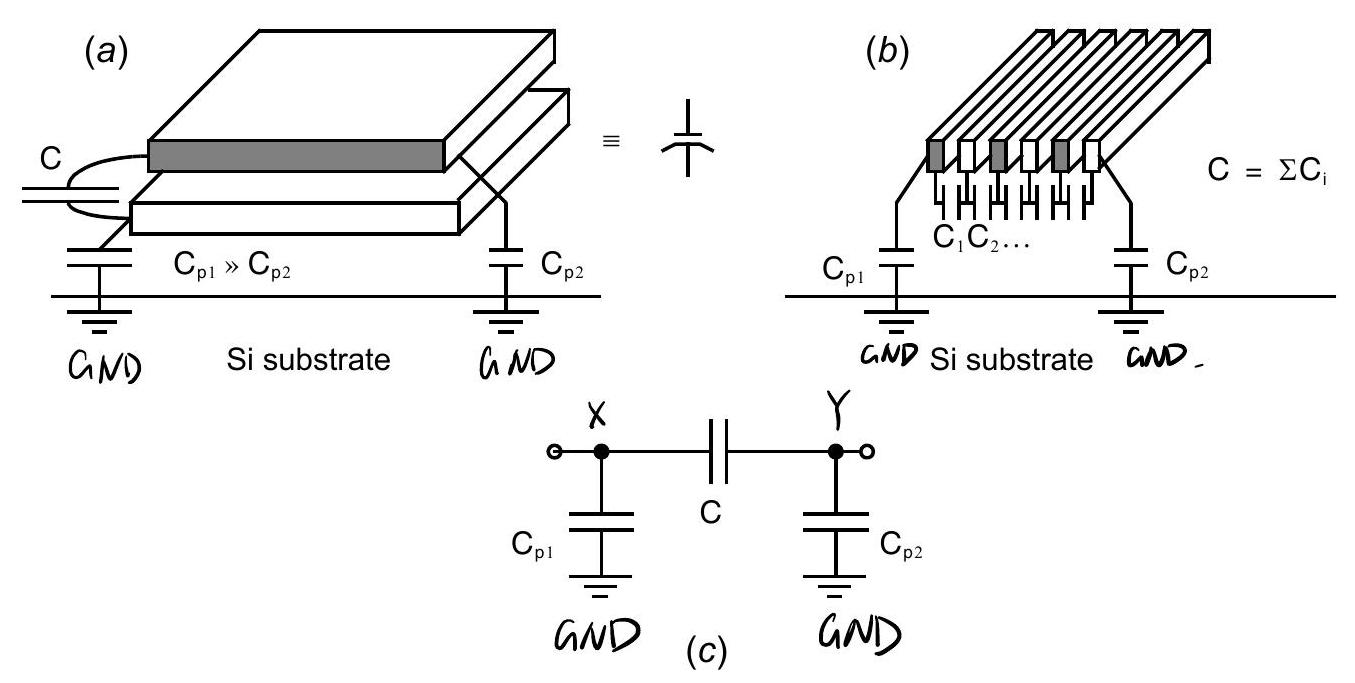
\includegraphics[max width=\textwidth, center]{2024_10_31_60860e27b87166db2267g-084}

Fig. 1.37 Metal-metal capacitor geometries: (a) parallel plate capacitor; (b) side-wall capacitors; (c) small-signal model.

When using either of these geometries, parasitics are minimized by locating them as high above the silicon substrate as possible. Of course, this may not be possible - for example, when a double-poly capacitor is being used. Furthermore, either of these geometries, or combinations of them, may be stacked on top of each other. For example, several parallel-plates may be stacked on top of each other with alternating layers shorted to provide a metal "sandwich" capacitor. Such complex structures generally provide even higher capacitance per unit area, and require the use of computer tools to accurately estimate their value.

\subsection*{1.7 APPENDIX}
The purpose of this appendix is to present derivations for device equations that rely heavily on device physics knowledge. Specifically, equations are derived for the exponential relationship and diffusion capacitance of diodes, and for the threshold voltage and triode relationship for MOS transistors.

\subsection*{1.7.1 Diode Exponential Relationship}
The concentration of minority carriers in the bulk, far from the junction, is given by (1.2) and (1.4). Close to the junction, the minority-carrier concentrations are much larger. Indeed, the concentration next to the junction increases exponentially with the external voltage, $\mathrm{V}_{\mathrm{D}}$, that is applied in the forward direction. The concentration of holes in the n side next to the junction, $\mathrm{p}_{\mathrm{n}}$, is given by [Sze, 1981]


\begin{equation*}
p_{n}=p_{n 0} e^{v_{D} v_{T}}=\frac{n_{i}^{2}}{N_{D}} e^{v_{D} / v_{T}} \tag{1.138}
\end{equation*}


Similarly, the concentration of electrons in the p side next to the junction is given by


\begin{equation*}
n_{p}=n_{p 0} e^{v_{D} / v_{T}}=\frac{n_{i}^{2}}{N_{A}} e^{v_{D} V_{T}} \tag{1.139}
\end{equation*}


As the carriers diffuse away from the junction, their concentration exponentially decreases. The relationship for holes in the n side is


\begin{equation*}
p_{n}(x)=p_{n}(0) e^{-x / L_{p}} \tag{1.140}
\end{equation*}


where x is the distance from the junction and $\mathrm{L}_{\mathrm{p}}$ is a constant known as the diffusion length for holes in the n side. Similarly, for electrons in the $p$ side we have


\begin{equation*}
n_{p}(x)=n_{p}(0) e^{-x / L_{n}} \tag{1.141}
\end{equation*}


where $L_{n}$ is a constant known as the diffusion length of electrons in the $p$ side. Note that $p_{n}(0)$ and $n_{p}(0)$ are given by (1.138) and (1.139), respectively. Note also that the constants $L_{n}$ and $L_{p}$ are dependent on the doping concentrations $\mathrm{N}_{\mathrm{A}}$ and $\mathrm{N}_{\mathrm{D}}$, respectively.

The current density of diffusing carriers moving away from the junction is given by the well-known diffusion equations [Sze, 1981]. For example, the current density of diffusing electrons is given by


\begin{equation*}
J_{D-n}=-q D_{n} \frac{d n_{p}(x)}{d x} \tag{1.142}
\end{equation*}


where $D_{n}$ is the diffusion constant of electrons in the $p$ side of the junction. The negative sign is present because electrons have negative charge. Note that $D_{n}(k T / q) \mu_{n}$, where $\mu_{n}$ is the mobility of electrons. Using (1.141), we have


\begin{equation*}
\frac{d n_{p}(x)}{d x}=\frac{n_{p}(0)}{L_{n}} e^{-x / L_{n}}=-\frac{n_{p}(x)}{L_{n}} \tag{1.143}
\end{equation*}


Therefore


\begin{equation*}
J_{D-n}=\frac{q D_{n}}{L_{n}} n_{p}(x) \tag{1.144}
\end{equation*}


Thus, the current density due to diffusion is proportional to the minority-carrier concentration. Next to the junction, all the current flow results from the diffusion of minority carriers. Further away from the junction, some of the current flow is due to diffusion and some is due to majority carriers drifting by to replace carriers that recombined with minority carriers or diffused across the junction.

Continuing, we use (1.139) and (1.144) to determine the current density next to the junction of electrons in the p side:


\begin{align*}
J_{D-n} & =\frac{q D_{n}}{L_{n}} n_{p}(0) \\
& =\frac{q D_{n}}{L_{n}} \frac{n_{i}^{2}}{N_{A}} e^{v_{D} / v_{T}} \tag{1.145}
\end{align*}


For the total current of electrons in the p side, we multiply (1.145) by the effective junction area, $\mathrm{A}_{\mathrm{D}}$. The total current remains constant as we move away from the junction since, in the steady state, the minority carrier concentration at any particular location remains constant with time. In other words, if the current changed as we moved away from the junction, the charge concentrations would change with time.

Using a similar derivation, we obtain the total current of holes in the n side, $\mathrm{I}_{\mathrm{D}-\mathrm{p}}$, as


\begin{equation*}
I_{D-p}=\frac{A_{D} q D_{n} n_{i}^{2}}{L_{p} N_{D}} e^{v_{D} v_{T}} \tag{1.146}
\end{equation*}


where $D_{n}$ is the diffusion constant of electrons in the $p$ side of the junction, $L_{p}$ is the diffusion length of holes in the n side, and $\mathrm{N}_{\mathrm{D}}$ is the impurity concentration of donors in the n side. This current, consisting of positive carriers, flows in the direction opposite to that of the flow of minority electrons in the p side. However, since electron carriers are negatively charged, the direction of the current flow is the same. Note also that if the p side is more heavily doped than the n side, most of the carriers will be holes, whereas if the n side is more heavily doped than the p side, most of the carriers will be electrons.

The total current is the sum of the minority currents at the junction edges:


\begin{equation*}
I_{D}=A_{D} q n_{i}^{2}\left(\frac{D_{n}}{L_{n} N_{A}}+\frac{D_{p}}{L_{p} N_{D}}\right) e^{v_{D} / v_{T}} \tag{1.147}
\end{equation*}


Equation (1.147) is often expressed as


\begin{equation*}
I_{D}=I_{S} e^{V_{D} V_{T}} \tag{1.148}
\end{equation*}


where


\begin{equation*}
I_{S}=A_{D} q n_{i}^{2}\left(\frac{D_{n}}{L_{n} N_{A}}+\frac{D_{p}}{L_{p} N_{D}}\right) \tag{1.149}
\end{equation*}


Equation (1.148) is the well-known exponential current-voltage relationship of forward-biased diodes.\\
The concentrations of minority carriers near the junction and the direction of current flow are shown in Fig. 1.38.

\subsection*{1.7.2 Diode-Diffusion Capacitance}
To find the diffusion capacitance, $\mathrm{C}_{\mathrm{d}}$, we first find the minority charge close to the junction, $\mathrm{Q}_{\mathrm{d}}$, and then differentiate it with respect to $\mathrm{V}_{\mathrm{D}}$. The minority charge close to the junction, $\mathrm{Q}_{\mathrm{d}}$, can be found by integrating either (1.140) or (1.141) over a few diffusion lengths. For example, if we assume $\mathrm{n}_{\mathrm{p} 0}$, the minority electron concentration in the $p$ side far from the junction is much less than $n_{p}(0)$, the minority electron concentration at the junction edge, we can use (1.141) to obtain


\begin{align*}
Q_{n} & =q A_{D} \int_{0}^{\infty} n_{p}(x) d x \\
& =q A_{D} \int_{0}^{\infty} n_{p}(0) e^{-x / L_{n}} d x  \tag{1.150}\\
& =q A_{D} L_{n} n_{p}(0)
\end{align*}


\begin{center}
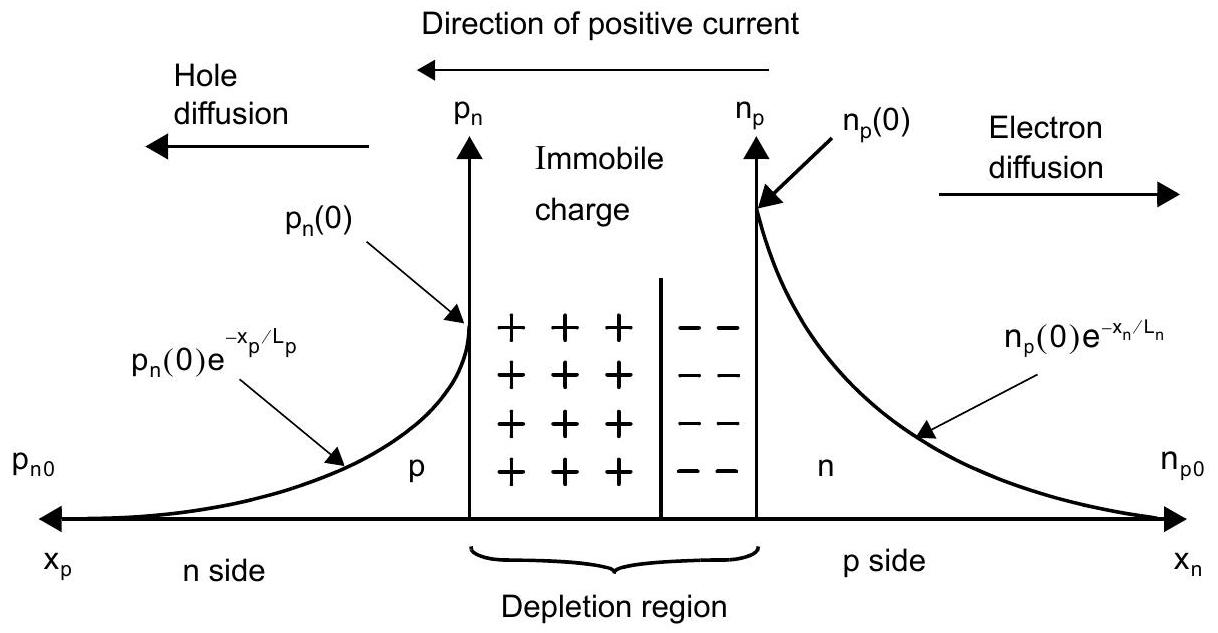
\includegraphics[max width=\textwidth]{2024_10_31_60860e27b87166db2267g-087}
\end{center}

Fig. 1.38 The concentration of minority carriers and the direction of diffusing carriers near a forward-biased junction.

Using for $\mathrm{n}_{\mathrm{p}}(0)$ results in


\begin{equation*}
Q_{n}=\frac{q A_{D} L_{n} n_{i}^{2}}{N_{A}} e^{v_{D} / v_{T}} \tag{1.151}
\end{equation*}


In a similar manner, we also have


\begin{equation*}
Q_{p}=\frac{q A_{D} L_{n} n_{i}^{2}}{N_{D}} e^{v_{D} / v_{T}} \tag{1.152}
\end{equation*}


For a typical junction, one side will be much more heavily doped than the other side, and therefore the minority charge storage in the heavily doped side can be ignored since it will be much less than that in the lightly doped side. Assuming the n side is heavily doped, we find the total charge, $\mathrm{Q}_{\mathrm{d}}$, to be approximately given by $\mathrm{Q}_{\mathrm{n}}$, the minority charge in the $p$ side. Thus, the small-signal diffusion capacitance, $C_{d}$, is given by


\begin{equation*}
C_{d}=\frac{d Q_{d}}{d V_{D}} \cong \frac{d Q_{n}}{d V_{D}}=\frac{q A_{D} L_{n} n_{i}^{2}}{N_{A} V_{T}} e^{v_{D} / V_{T}} \tag{1.153}
\end{equation*}


Using (1.147) and again noting that $\mathrm{N}_{\mathrm{D}} \gg \mathrm{N}_{\mathrm{A}}$, we have


\begin{equation*}
C_{d}=\frac{L_{n}^{2}}{D_{n}} \frac{I_{D}}{V_{T}} \tag{1.154}
\end{equation*}


Equation (1.154) is often expressed as


\begin{equation*}
C_{d}=\tau_{T} \frac{I_{D}}{V_{T}} \tag{1.155}
\end{equation*}


where $\tau_{T}$ is the transit time of the diode given by


\begin{equation*}
\tau_{T}=\frac{L_{n}^{2}}{D_{n}} \tag{1.156}
\end{equation*}


for a single-sided diode in which the n side is more heavily doped.

\subsection*{1.7.3 MOS Threshold Voltage and the Body Effect}
Many factors affect the gate-source voltage at which the channel becomes conductive. These factors are as follows:

\begin{enumerate}
  \item The work-function difference between the gate material and the substrate material
  \item The voltage drop between the channel and the substrate required for the channel to exist
  \item The voltage drop across the thin oxide required for the depletion region, with its immobile charge, to exist
  \item The voltage drop across the thin oxide due to unavoidable charge trapped in the thin oxide
  \item The voltage drop across the thin oxide due to implanted charge at the surface of the silicon. The amount of implanted charge is adjusted in order to realize the desired threshold voltage.
\end{enumerate}

The first factor affecting the transistor threshold voltage, $\mathrm{V}_{\mathrm{t}}$, is the built-in Fermi potential due to the different materials and doping concentrations used for the gate material and the substrate material. If one refers these potentials to that of intrinsic silicon [Tsividis, 1987], we have


\begin{equation*}
\phi_{\mathrm{F}-\text { Gate }}=\frac{\mathrm{kT}}{\mathrm{q}} \ln \left(\frac{\mathrm{~N}_{\mathrm{D}}}{\mathrm{n}_{\mathrm{i}}}\right) \tag{1.157}
\end{equation*}


for a polysilicon gate with doping concentration $N_{D}$, and


\begin{equation*}
\phi_{\mathrm{F} \text {-sub }}=\frac{\mathrm{kT}}{\mathrm{q}} \ln \left(\frac{\mathrm{n}_{\mathrm{i}}}{\mathrm{~N}_{\mathrm{A}}}\right) \tag{1.158}
\end{equation*}


for a p substrate with doping concentration $\mathrm{N}_{\mathrm{A}}$. The work-function difference is then given by


\begin{align*}
\phi_{\mathrm{MS}} & =\phi_{\mathrm{F} \text {-Sub }}-\phi_{\mathrm{F}-\mathrm{Gate}} \\
& =\frac{\mathrm{kT}}{\mathrm{q}} \ln \left(\frac{\mathrm{~N}_{\mathrm{D}} \mathrm{~N}_{\mathrm{A}}}{\mathrm{n}_{\mathrm{i}}^{2}}\right) \tag{1.159}
\end{align*}


The next factor that determines the transistor threshold voltage is the voltage drop from the channel to the substrate, which is required for the channel to exist. The question of exactly when the channel exists does not have a precise answer. Rather, the channel is said to exist when the concentration of electron carriers in the channel is equal to the concentration of holes in the substrate. At this gate voltage, the channel is said to be inverted. As the gate voltage changes from a low value to the value at which the channel becomes inverted, the voltage drop in the silicon also changes, as does the voltage drop in the depletion region between the channel and the bulk. After the channel becomes inverted, any additional increase in gate voltage is closely equal to the increase in voltage drop across the thin oxide. In other words, after channel inversion, gate voltage variations have little effect on the voltage drop in the silicon or the depletion region between the channel and the substrate.

The electron concentration in the channel is equal to the hole concentration in the substrate when the voltage drop from the channel to the substrate is equal to two times the difference between the Fermi potential of the substrate and intrinsic silicon, $\phi_{\mathrm{F}}$, where


\begin{equation*}
\phi_{F}=-\frac{\mathrm{kT}}{\mathrm{q}} \ln \left(\frac{\mathrm{~N}_{\mathrm{A}}}{\mathrm{n}_{\mathrm{i}}}\right) \tag{1.160}
\end{equation*}


Equation (1.200) is a factor in several equations used in modelling MOS transistors. For typical processes, $\phi_{F}$ can usually be approximated as 0.35 V for typical doping levels at room temperature.

The third factor that affects the threshold voltage is due to the immobile negative charge in the depletion region left behind after the p mobile carriers are repelled. This effect gives rise to a voltage drop across the thin oxide of $-Q_{B} / C_{o x}$, where


\begin{equation*}
Q_{B}=-q N_{A} x_{d} \tag{1.161}
\end{equation*}


and $x_{d}$ is the width of the depletion region. Since


\begin{equation*}
\mathrm{x}_{\mathrm{d}}=\sqrt{\frac{2 \mathrm{~K}_{\mathrm{s}} \varepsilon_{0} \mid 2 \phi_{\mathrm{F}}}{\mathrm{qN}_{\mathrm{A}}}} \tag{1.162}
\end{equation*}


we have


\begin{equation*}
\mathrm{Q}_{\mathrm{B}}=-\sqrt{2 \mathrm{qN}_{\mathrm{A}} \mathrm{~K}_{\mathrm{s}} \varepsilon_{0}\left|2 \phi_{\mathrm{F}}\right|} \tag{1.163}
\end{equation*}


The fourth factor that determines $\mathrm{V}_{\mathrm{tn}}$ is due to the unavoidable charge trapped in the thin oxide. Typical values for the effective ion density of this charge, $\mathrm{N}_{\mathrm{OX}}$, might be $2 \times 10^{14}$ to $10^{15} \mathrm{ions} / \mathrm{m}^{3}$. These ions are almost always positive. This effect gives rise to a voltage drop across the thin oxide, $\mathrm{V}_{\mathrm{ox}}$, given by


\begin{equation*}
V_{o x}=\frac{-Q_{o x}}{C_{o x}}=\frac{-q N_{o x}}{C_{o x}} \tag{1.164}
\end{equation*}


The native transistor threshold voltage is the threshold voltage that would occur naturally if one did not include a special ion implant used to adjust the threshold voltage. This value is given by


\begin{equation*}
V_{\text {t-native }}=\phi_{\mathrm{MS}}-2 \phi_{\mathrm{F}}-\frac{\mathrm{Q}_{\mathrm{B}}}{\mathrm{C}_{\mathrm{ox}}}-\frac{\mathrm{Q}_{\mathrm{ox}}}{\mathrm{C}_{\mathrm{ox}}} \tag{1.165}
\end{equation*}


A typical native threshold value might be around -0.1 V . It should be noted that transistors that have native transistor threshold voltages are becoming more important in analog circuit design where they are used in transmission gates or in source-follower buffers.

The fifth factor that affects threshold voltage is a charge implanted in the silicon under the gate to change the threshold voltage from that given by (1.165) to the desired value, which might be between 0.2 to 0.7 V for an n-channel transistor.

For the case in which the source-to-substrate voltage is increased, the effective threshold voltage is increased. This is known as the body effect. The body effect occurs because, as the source-bulk voltage, $\mathrm{V}_{\mathrm{SB}}$, becomes larger, the depletion region between the channel and the substrate becomes wider, and therefore more immobile negative charge becomes uncovered. This increase in charge changes the third factor in determining the transistor threshold voltage. Specifically, instead of using (1.163) to determine $Q_{B}$, one should now use


\begin{equation*}
\left.Q_{B}=-\sqrt{2 q N_{A} K_{s} \varepsilon_{0}\left(V_{S B}+\left|2 \phi_{F}\right|\right.}\right) \tag{1.166}
\end{equation*}


If the threshold voltage when $\mathrm{V}_{\mathrm{SB}}=0$ is denoted $\mathrm{V}_{\mathrm{tn} 0}$, then, using (1.165) and (1.166), one can show that


\begin{align*}
\mathrm{V}_{\mathrm{tn}}= & \mathrm{V}_{\mathrm{tn} 0}+\Delta \mathrm{V}_{\mathrm{tn}} \\
& =\mathrm{V}_{\mathrm{tn} 0}+\frac{\sqrt{2 \mathrm{q} \mathrm{~N}_{\mathrm{A}} \mathrm{~K}_{\mathrm{s}} \varepsilon_{0}}}{\mathrm{C}_{\mathrm{ox}}}\left[\sqrt{\mathrm{~V}_{\mathrm{SB}}+\left|2 \phi_{\mathrm{F}}\right|}-\sqrt{\left|2 \phi_{\mathrm{F}}\right|}\right]  \tag{1.167}\\
& =\mathrm{V}_{\mathrm{tn} 0}+\gamma\left(\sqrt{\mathrm{V}_{\mathrm{SB}}+\left|2 \phi_{\mathrm{F}}\right|}-\sqrt{\left|2 \phi_{\mathrm{F}}\right|}\right)
\end{align*}


where


\begin{equation*}
\gamma=\frac{\sqrt{2 q \mathrm{~N}_{\mathrm{A}} \mathrm{~K}_{\mathrm{s}} \varepsilon_{0}}}{\mathrm{C}_{\mathrm{ox}}} \tag{1.168}
\end{equation*}


The factor $\gamma$ is often called the body-effect constant.

\subsection*{1.7.4 MOS Triode Relationship}
The current flow in a MOS transistor is due to drift current rather than diffusion current. This type of current flow is the same mechanism that determines the current in a resistor. The current density, J , is proportional to the electrical field, E, where the constant of proportionality, $\sigma$, is called the electrical permittivity. Thus,


\begin{equation*}
J=\sigma E \tag{1.169}
\end{equation*}


This constant for an $n$-type material is given by


\begin{equation*}
\sigma=q n_{n} \mu_{n} \tag{1.170}
\end{equation*}


where n is the concentration per unit volume of negative carriers and $\mu_{\mathrm{n}}$ is the mobility of electrons. Thus, the current density is given by


\begin{equation*}
\mathrm{J}=\mathrm{qn}_{\mathrm{n}} \mu_{\mathrm{n}} \mathrm{E} \tag{1.171}
\end{equation*}


\begin{center}
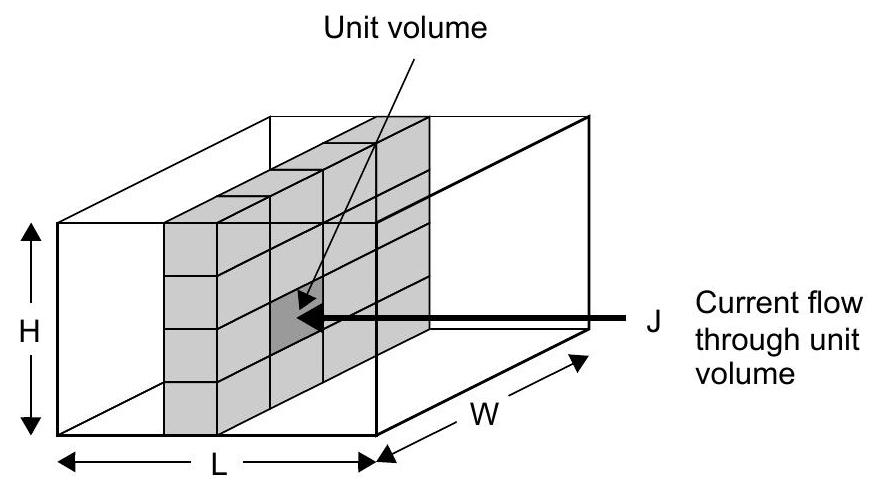
\includegraphics[max width=\textwidth]{2024_10_31_60860e27b87166db2267g-090}
\end{center}

Fig. 1.39 Current flowing through a unit volume.

Next, consider the current flow through the volume shown in Fig. 1.39, where the volume has height H and width W . The current is flowing perpendicular to the plane $\mathrm{H} \times \mathrm{W}$ down the length of the volume, L . The current, I, everywhere along the length of the volume is given by


\begin{equation*}
\mathrm{I}=\mathrm{JWH} \tag{1.172}
\end{equation*}


The voltage drop along the length of the volume in the direction of $L$ for a distance $d x$ is denoted $d V$ and is given by


\begin{equation*}
d V=E(x) d x \tag{1.173}
\end{equation*}


Combining (1.171), (1.172), and (1.173), we obtain


\begin{equation*}
\mathrm{q} \mu_{\mathrm{n}} \mathrm{WHn}_{\mathrm{n}}(\mathrm{x}) \mathrm{dV}=\mathrm{I} d \mathbf{x} \tag{1.174}
\end{equation*}


where the carrier density $n_{n}(x)$ is now assumed to change along the length $L$ and is therefore a function of $x$.\\
As an aside, we examine the case of a resistor where $n_{n}(x)$ is usually constant. A resistor of length $L$ would therefore have a current given by


\begin{equation*}
\mathrm{I}=\frac{\mathrm{q} \mu_{\mathrm{n}} \mathrm{WHn}}{\mathrm{~L}} \Delta \mathrm{~V} \tag{1.175}
\end{equation*}


Thus, the resistance is given by


\begin{equation*}
\mathrm{R}=\frac{\mathrm{L}}{\mathrm{q} \mu_{\mathrm{n}} \mathrm{WHn}_{\mathrm{n}}} \tag{1.176}
\end{equation*}


Often this resistance is presented in a relative manner, in which the length and width are removed (since they can be design parameters) but the height remains included. In this case, the resulting expression is commonly referred to as the resistance per square and designated as $\mathrm{R}_{\square}$ where


\begin{equation*}
R_{\square}=\frac{1}{q \mu_{n} H n_{n}} \tag{1.177}
\end{equation*}


The total resistance is then given by equation (1.133), repeated here for convenience.


\begin{equation*}
R_{\text {total }}=R_{\square} \frac{L}{W} \tag{1.178}
\end{equation*}


In the case of a MOS transistor, the charge density is not constant down the channel. If, instead of the carrier density per unit volume, one expresses $\mathrm{n}_{\mathrm{n}}(\mathrm{x})$ as a function of charge density per square area from the top looking down, we have


\begin{equation*}
\mathrm{Q}_{\mathrm{n}}(\mathrm{x})=\mathrm{qHn} \mathrm{n}_{\mathrm{n}}(\mathrm{x}) \tag{1.179}
\end{equation*}


Substituting (1.179) into (1.174) results in


\begin{equation*}
\mu_{n} W Q_{n}(x) d V=I d x \tag{1.180}
\end{equation*}


Equation (1.180) applies to drift current through any structure that has varying charge density in the direction of the current flow. It can also be applied to a MOS transistor in the triode region to derive its I-V relationship. It should be noted here that in this derivation, it is assumed the source voltage is the same as the substrate voltage.

Since the transistor is in the triode region, we have $\mathrm{V}_{\mathrm{DG}}<-\mathrm{V}_{\mathrm{tn}}$. This requirement is equivalent to $\mathrm{V}_{\mathrm{DS}}<\mathrm{V}_{\mathrm{GS}}-\mathrm{V}_{\mathrm{tn}}=\mathrm{V}_{\text {eff }}$. It is assumed that the effective channel length is L . Assuming the voltage in the channel at distance x from the source is given by $\mathrm{V}_{\mathrm{ch}}(\mathrm{x})$, from Fig. 1.40, we have


\begin{equation*}
Q_{n}(x)=C_{o x}\left[V_{G S}-V_{c h}(x)-V_{t n}\right] \tag{1.181}
\end{equation*}


Substituting (1.181) into (1.180) results in


\begin{equation*}
\mu_{\mathrm{n}} \mathrm{WC}_{\mathrm{ox}}\left[\mathrm{~V}_{\mathrm{GS}}-\mathrm{V}_{\mathrm{ch}}(\mathrm{x})-\mathrm{V}_{\mathrm{tn}}\right] \mathrm{d} \mathrm{~V}_{\mathrm{ch}}=\mathrm{I}_{\mathrm{D}} \mathrm{dx} \tag{1.182}
\end{equation*}


Integrating both sides of (1.182), and noting that the total voltage along the channel of length $L$ is $V_{D S}$, we obtain


\begin{equation*}
\int_{0}^{V_{D S}} \mu_{\mathrm{n}} \mathrm{WC}_{\mathrm{ox}}\left[\mathrm{~V}_{\mathrm{GS}}-\mathrm{V}_{\mathrm{ch}}(\mathrm{x})-\mathrm{V}_{\mathrm{tn}}\right] \mathrm{d} \mathrm{~V}_{\mathrm{ch}}=\int_{0}^{\mathrm{L}} \mathrm{I}_{\mathrm{D}} \mathrm{dx} \tag{1.183}
\end{equation*}


\begin{center}
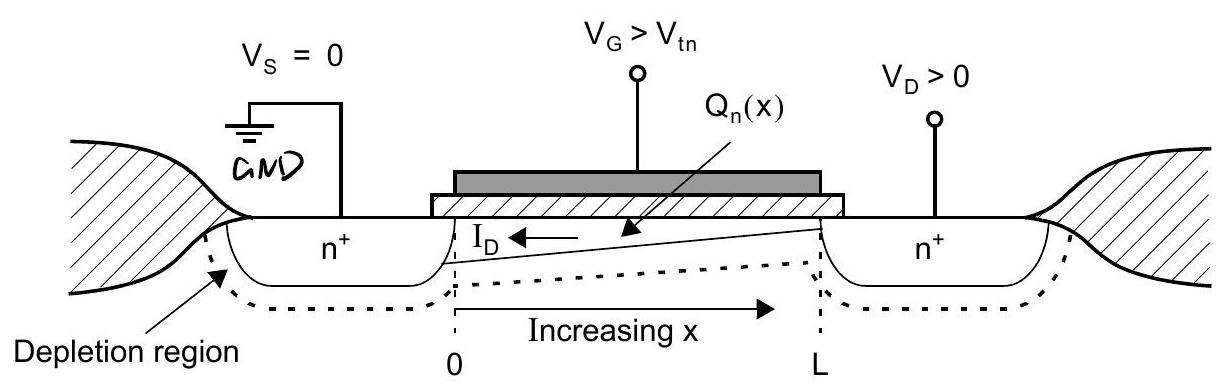
\includegraphics[max width=\textwidth]{2024_10_31_60860e27b87166db2267g-091}
\end{center}

Fig. 1.40 The transistor definitions used in developing the transistor's I-V relationship.\\
which results in


\begin{equation*}
\mu_{\mathrm{n}} \mathrm{WC}_{\mathrm{ox}}\left[\left(\mathrm{~V}_{\mathrm{GS}}-\mathrm{V}_{\mathrm{tn}}\right) \mathrm{V}_{\mathrm{DS}}-\frac{\mathrm{V}_{\mathrm{DS}}^{2}}{2}\right]=\mathrm{I}_{\mathrm{D}} \mathrm{~L} \tag{1.184}
\end{equation*}


Thus, solving for $I_{D}$ results in the well-known triode relationship for a MOS transistor:


\begin{equation*}
\mathrm{I}_{\mathrm{D}}=\mu_{\mathrm{n}} \mathrm{C}_{\mathrm{ox}}\left(\frac{\mathrm{~W}}{\mathrm{~L}}\right)\left[\left(\mathrm{V}_{\mathrm{GS}}-\mathrm{V}_{\mathrm{tn}}\right) \mathrm{V}_{\mathrm{DS}}-\frac{\mathrm{V}_{\mathrm{DS}}^{2}}{2}\right] \tag{1.185}
\end{equation*}


It should be noted that taking into account the body effect along the channel, the triode model of (1.225) is modified to


\begin{equation*}
\mathrm{I}_{\mathrm{D}}=\mu \mathrm{C}_{\mathrm{ox}}\left(\frac{\mathrm{~W}}{\mathrm{~L}}\right)\left[\left(\mathrm{V}_{\mathrm{GS}}-\mathrm{V}_{\mathrm{tn}}\right) \mathrm{V}_{\mathrm{DS}}-\alpha \frac{\mathrm{V}_{\mathrm{DS}}^{2}}{2}\right] \tag{1.186}
\end{equation*}


where $\alpha \cong 1.7$ [Tsividis, 1987].

\subsection*{1.8 KEY POINTS}
\begin{itemize}
  \item The charge-voltage relationship of a reverse-biased pn junction is modeled by a nonlinear depletion capacitance. [p. 6]
  \item The source terminal of an n-channel transistor is defined as whichever of the two terminals has a lower voltage. For a p-channel transistor, the source would be the terminal with the higher voltage. [p. 14]
  \item The relationship between drain-source voltage and drain current of a MOS device is approximately linear when $V_{D S}<<V_{\text {eff: }}$ [p. 19]
  \item For $\mathrm{V}_{\mathrm{DS}}>\mathrm{V}_{\text {eff }}$, a MOS device exhibits a square-law current-voltage relationship. [p. 21]
  \item The body effect is the influence of the body potential on the channel, modelled as an increase in the threshold voltage, $\mathrm{V}_{\mathrm{tn}}$, with increasing source-to-body reverse-bias. [p. 24]
  \item The square-root relationship for transconductance is useful for circuit analysis when device sizes are fixed. However, the simpler expression $\mathrm{g}_{\mathrm{m}}=2 \mathrm{I}_{\mathrm{D}} / \mathrm{V}_{\text {eff }}$ is useful during initial circuit design when transistor sizes are yet to be determined. [p. 26]
  \item Small signal $r_{d s}$ is proportional to $L / I_{D}$. [p. 28]
  \item In a MOSFET, the largest parasitic capacitance is $\mathrm{C}_{\mathrm{gs}}$, proportional to gate area WL and via $\mathrm{C}_{\mathrm{ox}}$ inversely proportional to oxide thickness. [p. 31]
  \item The gate-drain capacitance $\mathrm{C}_{\mathrm{gd}}$, also known as the Miller capacitance, is due to physical overlap of the gate and drain regions as well as fringing fields. It is especially important when there is a large voltage gain between gate and drain. [p. 32]
  \item For operation with high gain, transistors should have long gate lengths and be biased with low $\mathrm{V}_{\text {eff }}$. For high speed, the opposite is desirable: small L and high $\mathrm{V}_{\mathrm{eff}}$ [p.38]
  \item In subthreshold operation, also called weak inversion, transistors obey an exponential voltage-current relationship instead of a square-law. Hence, a small but finite current flows even when $\mathrm{V}_{\mathrm{GS}}=0$. [p. 42]
  \item For a fixed drain current, the small-signal transconductance of a MOS device is maximized in subthreshold operation at a value of $\mathrm{g}_{\mathrm{m}}=\mathrm{qI}_{\mathrm{D}} / \mathrm{nkT}$. [p. 43]
  \item For large values of $\mathrm{V}_{\text {eff }}$, transistors have a sub-square-law voltage current relationship, tending towards a linear relationship for very large values of $\mathrm{V}_{\text {eff: }}$ [p.46]
\end{itemize}

\subsection*{1.9 REFERENCES}
R. Geiger, P. Allen, and N. Strader. VLSI: Design Techniques for Analog and Digital Circuits. McGraw-Hill, New York, 1990.\\
P. Gray, P. J. Hurst, S. H. Lewis, and R. G. Meyer. Analysis and Design of A nalog In tegrated Circuits, 5th. ed. John Wiley \& Sons, New York, 2009.\\
D. Hodges and H. Jackson. Analysis and Design of Digital Integrated Circuits, 2nd ed. McGraw-Hill, New York, 1988.\\
D. Roulston. Semiconductor Devices. McGraw-Hill, New York, 1990.\\
C. G. Sodini, P.-K. Ko, and J. L. Moll, "The effect of High Fields on MOS Device and Circuit Performance," IEEE Trans. Electron Devices, Vol. 31, pp. 1386-1393, October 1984.\\
S. M. Sze. Physics of Semiconductor Devices. Wiley Interscience, New York, 1981.\\
Y. Tsividis. Operation and Modeling of the MOS Transistor. McGraw-Hill, New York, 1987.\\
S. Wolf. Silicon Processing for the VLSI Era-Volume 3: The Submicron MOSFET. Lattice Press, Sunset Beach, California, 1995.

\subsection*{1.10 PROBLEMS}
\subsection*{1.10.1 Section 1.1: Semiconductors and pn Junctions}
1.1 Estimate the hole and electron concentrations in silicon doped with arsenic at a concentration of $10^{25}$ atoms $/ \mathrm{m}^{3}$ at a temperature $22^{\circ} \mathrm{C}$ above room temperature. Is the resulting material n type or p type?\\
1.2 For the pn junction of Example 1.2, estimate the new built-in potential, $\Phi_{0}$, when the temperature is increased $11^{\circ} \mathrm{C}$ above room temperature.\\
1.3 Calculate the amount of charge per $(\mu \mathrm{m})^{2}$ in each of the n and p regions of the pn junction of Example 1.2 for a 3-V reverse-bias voltage. How much charge on each side would be present in a $10 \mu \mathrm{~m} \times 10 \mu \mathrm{~m}$ diode?\\
1.4 A silicon diode has $\mathrm{C}_{\mathrm{j} 0}=15 \mathrm{fF}$. It is biased by a $43-\mathrm{k} \Omega$ resistor connected between the cathode of the diode and the input signal, as shown in Fig. P1.4. Initially, the input is 3 V , and then at time 0 it changes to 0 V . Estimate the time it takes for the output voltage to change from 3 V to 0.9 V (i.e., the $\Delta \mathrm{t}_{-70 \%}$ time). Repeat for an input voltage change from 0 V to 3 V and an output voltage change from 0 V to 2.1 V . Compare your answers to those obtained using a SPICE simulation.\\
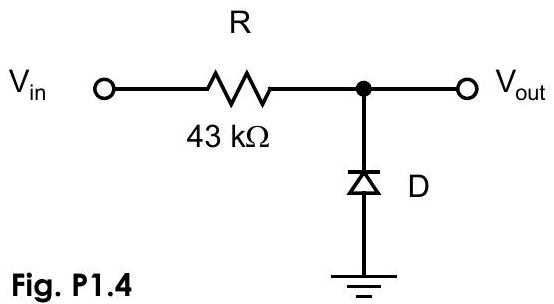
\includegraphics[max width=\textwidth, center]{2024_10_31_60860e27b87166db2267g-093}\\
1.5 Sketch a plot of the electric field strength versus depth for the pn junction of Example 1.3.\\
1.6 At what reverse-bias voltage will the pn junction of Example 1.3 breakdown? Assume that when the electric field exceeds $3 \times 10^{7} \mathrm{~V} / \mathrm{m}$, avalanche breakdown occurs.\\
1.7 A pn junction with $\mathrm{N}_{\mathrm{A}}$ « $\mathrm{N}_{\mathrm{D}}$ and an area $40 \mu \mathrm{~m}^{2}$ is observed to have a capacitance of 30 fF while under 1-V reverse bias. Estimate the dopant concentration on the p side, $\mathrm{N}_{\mathrm{A}}$.

\subsection*{1.10.2 Section 1.2: MOS Transistors and Section 1.3: Device Model Summary}
1.8 Verify that when $V_{D S}=V_{\text {eff }}$ is used in the triode equation for a MOS transistor, the current equals that of the active region equation given in (1.63).\\
1.9 Find $I_{D}$ for an $n$-channel transistor having doping concentrations of $N_{D}=10^{26}$ atoms $/ \mathrm{m}^{3}$ and $\mathrm{N}_{\mathrm{A}}=10^{23}$ atoms $/ \mathrm{m}^{3}$ with $\mathrm{W}=5 \mu \mathrm{~m}, \mathrm{~L}=0.5 \mu \mathrm{~m}, \mathrm{~V}_{\mathrm{GS}}=1 \mathrm{~V}$, and $\mathrm{V}_{\mathrm{DS}}=\mathrm{V}_{\text {eff }}$. Assuming $\lambda$ remains constant, estimate the new value of $I_{D}$ if $V_{D S}$ is increased by 0.3 V .\\
1.10 A MOS transistor in the active region is measured to have a drain current of $20 \mu \mathrm{~A}$ when $\mathrm{V}_{\mathrm{DS}}=\mathrm{V}_{\text {eff }}$. When $V_{D S}$ is increased by $0.5 \mathrm{~V}, I_{D}$ increases to $23 \mu \mathrm{~A}$. Estimate the output impedance, $r_{d s}$, and the output impedance constant, $\lambda$.\\
1.11 Derive the low-frequency model parameters for an n -channel transistor having doping concentrations of $\mathrm{N}_{\mathrm{D}}=10^{26}$ atoms $/ \mathrm{m}^{3}$ and $\mathrm{N}_{\mathrm{A}}=10^{23}$ atoms $/ \mathrm{m}^{3}$ with $\mathrm{W}=8 \mu \mathrm{~m}, \mathrm{~L}=0.6 \mu \mathrm{~m}, \mathrm{~V}_{\mathrm{GS}}=0.9 \mathrm{~V}$, and $\mathrm{V}_{\mathrm{DS}}=\mathrm{V}_{\text {eff }}$. Assume that $\mathrm{V}_{\mathrm{SB}}=1.0 \mathrm{~V}$.\\
1.12 Find the capacitances $C_{g s}, C_{g d}, C_{d b}$, and $C_{s b}$ for an active $n$-channel transistor having doping concentrations of $\mathrm{N}_{\mathrm{D}}=10^{26}$ atoms $/ \mathrm{m}^{3}$ and $\mathrm{N}_{\mathrm{A}}=10^{23}$ atoms $/ \mathrm{m}^{3}$ with $\mathrm{W}=15 \mu \mathrm{~m}, \mathrm{~L}=0.5 \mu \mathrm{~m}$. Assume that the source and drain junctions extend $1 \mu \mathrm{~m}$ beyond the gate, resulting in source and drain areas being $A_{s}=A_{d}=15 \mu \mathrm{~m}^{2}$ and the perimeter of each being $P_{s}=P_{d}=32 \mu \mathrm{~m}$.\\
1.13 Consider the circuit shown in Fig. P1.13, where $\mathrm{V}_{\text {in }}$ is a dc signal of 1 V . Taking into account only the channel charge storage, determine the final value of $\mathrm{V}_{\text {out }}$ when the transistor is turned off, assuming half the channel charge goes to $\mathrm{C}_{\mathrm{L}}$. You may use the parameters for the $0.18-\mu \mathrm{m}$ CMOS processes in Table 1.5.\\
\includegraphics[max width=\textwidth, center]{2024_10_31_60860e27b87166db2267g-094}\\
1.14 For the same circuit as in Problem 1.13, the input voltage has a step voltage change at time 0 from 0.2 V to 0.4 V (the gate voltage remains at 1.8 V ). Find its 99 percent settling time (the time it takes to settle to within 1 percent of the total voltage change). You may ignore the body effect and all capacitances except $\mathrm{C}_{\mathrm{L}}$. Repeat the question for $\mathrm{V}_{\text {in }}$ changing from 0.6 V to 0.8 V .\\
1.15 Repeat Problem 1.14, but now take into account the body effect on $\mathrm{V}_{\mathrm{tn}}$. Assume $\mathrm{N}_{\mathrm{A}}=10^{23}$ atoms $/ \mathrm{m}^{3}$.\\
1.16 For each of the CMOS processes tabulated in Table 1.5 , how many charge carriers $q$ are required to elevate the gate voltage of a triode MOSFET by 100 mV ? Assume that the gate length L is the minimum permitted in each technology and $W / L=20$.\\
1.17 Using the device parameters for the $0.35-\mu \mathrm{m}$ technology NMOS device in Table 1.5 and $\mathrm{L}=0.4 \mu \mathrm{~m}$, select the device width and $V_{G S}$ required to bias a transistor with an intrinsic gain of $A_{i}=10$ and transconductance $\mathrm{g}_{\mathrm{m}}=0.5 \mathrm{~mA} / \mathrm{V}$. What dc current consumption is required?\\
1.18 Repeat Problem 1.18 using the device parameters for the $0.18-\mu \mathrm{m}$ technology PMOS device in Table 1.5 and $\mathrm{L}=0.2 \mu \mathrm{~m}$.\\
1.19 A NMOS transistor is to be biased with $\mathrm{V}_{\text {eff }}=250 \mathrm{mV}$. Size the transistor using the device parameters for the $0.35-\mu \mathrm{m}$ CMOS process in Table 1.5 to provide a drain current of 0.2 mA and an output resistance of $r_{d s}=20 \mathrm{k} \Omega$. Repeat for a PMOS transistor. Repeat for the $0.18-\mu \mathrm{m}$ CMOS process.\\
1.20 A NMOS transistor is to be biased with $\mathrm{I}_{\mathrm{D}}=0.35 \mathrm{~mA}$ and an intrinsic gain of $\mathrm{A}_{\mathrm{i}}=35$ in the $0.35-\mu \mathrm{m}$ CMOS process in Table 1.5. Find the required transistor dimentions, W and L .\\
1.21 A NMOS transistor is to be biased with $\mathrm{I}_{\mathrm{D}}=0.25 \mathrm{~mA}$ and transconductance of $\mathrm{g}_{\mathrm{m}}=2.2 \mathrm{~mA} / \mathrm{V}$ in the $0.18-\mu \mathrm{m}$ CMOS process in Table 1.5. Find the required transistor dimentions, W and L .\\
1.22 Consider the circuit in Fig. P1.13. Size the NMOS transistor so that, with $\mathrm{V}_{\text {in }}=\mathrm{V}_{\text {out }}=0.3 \mathrm{~V}$, the circuit has a bandwidth of 250 MHz . Use the device parameters for the $0.35-\mu \mathrm{m}$ technology in Table 1.5. Assume $\mathrm{L}=0.35 \mu \mathrm{~m}$ and the threshold voltage is increased by 70 mV due to the body effect. What is the resulting gate capacitance?\\
1.23 Repeat Problem 1.22, this time using the device parameters for the $0.18-\mu \mathrm{m}$ technology in Table 1.5 with $\mathrm{L}=0.18 \mu \mathrm{~m}$.

\subsection*{1.10.3 Section 1.4: Advanced MOS Modelling and Section 1.5: SPICE Modelling Parameters}
1.24 If transistor drain current is plotted versus gate-source voltage on a log-log scale, what is the slope of the curve in strong inversion? What is the slope for very large values of $\mathrm{V}_{\mathrm{Gs}}$ ? What is the slope of the curve at $\mathrm{V}_{\text {eff }}=1 / \theta$ ?\\
1.25 Make a qualitative sketch of transistor intrinsic gain, $A_{i}$, versus $V_{\text {eff }}$ for:\\
a. constant device width, W\\
b. constant drain current, $I_{D}$

In each case, what is the relationship between $A_{i}$ and $V_{\text {eff }}$ in weak-inversion, active mode, and under mobility degradation?\\
1.26 Derive expressions for transistor $f_{T}$ in terms of fundamental device constants and operating point while operating in subthreshold and under mobility degradation. How do these compare with the expressions for strong inversion?\\
1.27 Using the Spice models from the text web site, perform simulations to extract approximate values for all of the transistor parameters listed in Table 1.5. Compare your results to the values in the table.\\
1.28 Two transistors with the same device paramters are biased with the same terminal voltages and have the same gate length $L$.\\
\includegraphics[max width=\textwidth, center]{2024_10_31_60860e27b87166db2267g-095}\\
a. One of the transistors has a drain current $\mathrm{I}_{\mathrm{D}}=0.2 \mathrm{~mA}$ and a width of $\mathrm{W}=3 \mu \mathrm{~m}$. Find the width of the other transistor so that it has a transconductance $I_{D}=2 \mathrm{~mA}$.\\
b. One of the transistors has a transconductance $\mathrm{g}_{\mathrm{m}}=0.4 \mathrm{~mA} / \mathrm{V}$ and a width of $\mathrm{W}=2 \mu \mathrm{~m}$. Find the width of the other transistor so that it has a transconductance $g_{m}=2 \mathrm{~mA} / \mathrm{V}$.\\
c. One of the transistors has a small-signal $r_{\mathrm{ds}}=1 \mathrm{k} \Omega$ and a width of $\mathrm{W}=30 \mu \mathrm{~m}$. Find the width of the other transistor so that it has a small-signal $\mathrm{r}_{\mathrm{ds}}=10 \mathrm{k} \Omega$.

\subsection*{1.10.4 Section 1.6: Passive Devices}
1.29 Assume a strip resistor has a sheet resistance of $1 \mathrm{k} \Omega / \mathrm{sq}$. and a total capacitance to ground of approximately $0.4 \mathrm{fF} / \mu \mathrm{m}^{2}$. What is the RC time constant formed by a $4 \mathrm{k} \Omega$ resistor with one end grounded assuming the resistor is $1 \mu \mathrm{~m}$ wide? What if it is only $0.4 \mu \mathrm{~m}$ wide? How does this compare with the time constant obtained using the n -well resistor in Example 1.20?\\
1.30 A reverse-biased pn junction with $\mathrm{N}_{\mathrm{D}}=10^{26}$ atoms $/ \mathrm{m}^{3}$ and $\mathrm{N}_{\mathrm{A}}=10^{23}$ atoms $/ \mathrm{m}^{3}$ is to be used as a varactor. What junction area and voltage range is needed to provide a capacitance tunable from 0.2 pF to 0.3 pF ?\\
1.31 In a particular process, a metal-metal parallel plate capacitor can be realized with a density of $7 \mathrm{fF} / \mu \mathrm{m}^{2}$ and a metal-metal sidewall capacitor can provide a density of $10 \mathrm{fF} / \mu \mathrm{m}^{2}$. What would be the area of a 1 pF capacitor realized using each approach? Compare this with the area of a 1 pF MOS capacitor in a $45-\mathrm{nm}$ CMOS processes using the parameters in Table 1.5.\\
1.32 Estimate the maximum percentage change in capacitance achievable using a MOS varactor in the $0.18-\mu \mathrm{m}$ CMOS processes in Table 1.5.

\section*{Processing and Layout}
This chapter describes the steps and processes used in realizing modern integrated circuits with emphasis on CMOS processing. After processing is presented, circuit layout is covered. Layout is the design portion of integrated-circuit manufacturing, in which the geometry of circuit elements and wiring connections is defined. This process leads to the development of photographic masks used in manufacturing an integrated circuit. The concepts of design rules and their relationship to integrated circuits are emphasized. Next, circuit layout is related to the transistor models. Here, it is shown that once the layout is completed, the values of certain elements in the transistor models can be determined. This knowledge is necessary for accurate computer simulation of integrated circuits. It is also shown that, by using typical design rules, one can make reasonable assumptions to approximate transistor parasitic components before the layout has been done. Variability in device parameters is unavoidable and particularly problematic for analog circuits. These variations are modeled and their impact on analog circuits analyzed. Finally, analog layout issues are then discussed, including matching and noise considerations.

\subsection*{2.1 CMOS PROCESSING}
In this section, the basic steps involved in processing a CMOS integrated circuit are presented. For illustrative purposes, we describe here an example n -well process with a p substrate and two layers of metal. Many of the possible variations during processing are also described, but we focus primarily on the basics which any analog designer should know. The processing of nanometer feature sizes can require many additional steps.

\subsection*{2.1.1 The Silicon Wafer}
The first step in realizing an integrated circuit is to fabricate a defect-free, single-crystalline, lightly doped silicon wafer. To realize such a wafer, one starts by creating metallurgical-grade silicon through the use of a high-temperature chemical process in an electrode-arc furnace. Although metallurgical-grade silicon is about 98 percent pure, it has far too many impurities for use in realizing integrated circuits. Next, a silicon-containing gas is formed and then reduced. Pure silicon is precipitated onto thin rods of single-crystalline silicon. This deposited electronic-grade silicon is very pure but, unfortunately, it is also polycrystalline. To obtain single-crystalline silicon, the silicon is melted once again and allowed to cool. As it cools, a single-crystalline ingot is slowly pulled and turned from the molten silicon using the Czochralski method. The Czochralski method starts with a seed of single crystal silicon, and the pull rate and speed of rotation determine the diameter of the crystalline rod or ingot. Typical diameters are 10 to 30 cm (i.e., 4 to 12 inches) with lengths usually longer than 1 meter. Producing a silicon ingot can take several days.

Key Point: The first step in realizing an integrated circuit is to produce a single-crystalline silicon wafer from 10 to 30 cm in diameter and roughly 1 mm thick. The silicon is either lightly doped, or heavily doped with a thin lightly-doped epitaxial layer on top in which the transistors are made.

Normally, heavily doped silicon is added to the melt before the singlecrystalline ingot is pulled. After the doped silicon diffuses through the molten silicon, a more lightly doped silicon ingot results. In our example process, boron impurities would be added to produce a p -type ingot. The ingot is cut into wafers using a large diamond saw. A typical wafer might have a thickness of about 1 mm . After the ingot is sawed into wafers, each wafer is polished with $\mathrm{Al}_{2} \mathrm{O}_{3}$, chemically etched to remove mechanically damaged material, and then fine-polished again with $\mathrm{SiO}_{2}$ particles in an aqueous solution of NaOH . Very often, the company that produces the silicon wafers is not the same company that eventually patterns them into monolithic circuits.

There are two methods for establishing the background doping level of the surface silicon in which all of the transistors will be made. One is to simply control the boron impurity levels in the ingot to provide a $\mathrm{p}^{-}$wafer concentration of around $\mathrm{N}_{\mathrm{A}} \cong 2 \times 10^{21}$ donor $/ \mathrm{m}^{3}$. Such a doping level would give a resistivity of 10 to $20 \Omega \cdot \mathrm{~cm}$. The other method is to begin with a very heavily doped $\mathrm{p}^{++}$wafer with a low resistivity of around $0.01 \Omega \cdot \mathrm{~cm}$. Then, upon the surface of the $\mathrm{p}^{++}$wafer, a layer of $\mathrm{p}^{-}$silicon is grown with a higher resistivity of 5 to $20 \Omega \cdot \mathrm{~cm}$. All of the devices are fabricated within this top epitaxial layer, which may be from 2 to $20 \mu \mathrm{~m}$ thick. The use of an epitaxial layer provides more precise control over dopant concentrations while the $\mathrm{p}^{++}$substrate underneath provides a low-resistivity ground plane under the circuit helping to prevent latchup, described in Section 2.2.4. In either case, transistors are fabricated in $\mathrm{p}^{-}$silicon near the surface of the wafer.

\subsection*{2.1.2 Photolithography and Well Definition}
Photolithography is a technique in which selected portions of a silicon wafer can be masked so that some type of processing step can be applied to the remaining areas. Although photolithography is used throughout the manufacture of an integrated circuit, here we describe this photographic process in the context of preparing the wafer for defining the well regions. ${ }^{1}$

Selective coverage for well definition is performed as follows. First, a glass mask, $\mathrm{M}_{1}$, is created, which defines where the well regions will be located. The glass mask is created by covering the mask in photographic materials and exposing it to an electron beam, or e beam, in the regions corresponding to the well locations. Such exposure results in the well regions on the glass mask turning opaque, or dark. As a result, the glass mask can be thought of as a negative of one layer of the microcircuit. In a typical microcircuit process, ten to twenty different masks might be required. The cost for these masks varies considerably depending upon the minimum feature sizes to be patterned on the microcircuit. For example, currently a set of masks for a $0.35-\mu \mathrm{m}$ CMOS process might cost roughly $\$ 30,000$, whereas the cost of a mask set for the most advanced modern processes approaches $\$ 1,000,000$. Because a high degree of precision is required in manufacturing these masks, often (but not always) a company other than the integrated circuit processing company makes the masks. The creation of the opaque regions of the mask by the electron beam is controlled by a computer dependent on the contents of a database. The database required for the e beam is derived from the layout database produced by the designer, using a computer-aided design (CAD) software program.

The first step in masking the surface of the wafer is to thermally grow a thin layer of silicon-dioxide $\left(\mathrm{SiO}_{2}\right)$ to protect the surface of the microcircuit. Details of this step are discussed later. On top of the $\mathrm{SiO}_{2}$, a negative photoresist, $\mathrm{PR}_{1}$, is evenly applied to a thickness of around $1 \mu \mathrm{~m}$ while spinning the microcircuit. Photoresist is a lightsensitive polymer (similar to latex). In the next step, the mask, $\mathrm{M}_{1}$, is placed in close proximity to the wafer, and ultraviolet light is projected through the mask onto the photoresist. Wherever the light strikes, the polymers crosslink, or polymerize. This change makes these regions insoluble to an organic solvent. This step is shown in Fig. 2.1

\footnotetext{\begin{enumerate}
  \item Wells are doped regions that will contain one of the two types of transistors realized in a CMOS process. For example, wells that are n type contain p -channel transistors.
\end{enumerate}
}Ultraviolet light\\
\includegraphics[max width=\textwidth, center]{2024_10_31_60860e27b87166db2267g-099}

Fig. 2.1 Se-lectively hardening a region of photoresist using a glass mask.\\
The regions where the mask was opaque (i.e., the well regions) are not exposed. The photoresist is removed in these areas using an organic solvent. Next, the remaining photoresist is baked to harden it. After the photoresist in the well regions is removed, the uncovered $\mathrm{SiO}_{2}$ may also be removed using an acid etch. (However, in some processes where this layer is very thin, it may not be removed.) In the next step, the dopants needed to form the well are introduced into the silicon using either diffusion or ion implantation (directly through the thin oxide, in cases where it has not been removed).

The procedure just described involves a negative photor esist, where the exposed photoresist remains after the masking. There are also positive photoresists, in which the exposed photoresist is dissolved by the organic solvents. In this case, the photoresist remains where the mask was opaque. By using both positive and negative resists, a single mask can sometimes be used for two steps-first, to protect one region and implant the complementary region and second, to protect the complementary region and implant the original region.

The feature sizes that may be patterned using photolithography are influenced by the wavelength of light used. When the integrated circuit features are smaller than the wavelength of light (currently 193-nm ultraviolet light is used),

Key Point: Most features on integrated circuits are patterned using photolithography whereby light is passed through a mask to cast patterns onto the underlying silicon wafer, ultimately defining the circuit's physical features such as transistor sizes and wiring.\\
the wave nature of light results in patterns on the photoresist that do not precisely match those of the mask. Fortunately, these effects can be partially compensated for by modifying the mask pattern so that the resulting geometries more closely match those intended by the designer. This technique is referred to as "optical proximity correction" and is a common practice to realize feature sizes below 100 nm . Further improvements have been made by immersing the photolithography in a liquid bath. Doing so changes the path of light resulting in improved resolution and improved tolerance to unevenness of the substrate surface. Efforts are ongoing to reduce the minimum feature sizes that may be patterned by using shorter wavelengths for photolithography (extreme ultraviolet light or even X-rays).

\subsection*{2.1.3 Diffusion and Ion Implantation}
After the photoresist over the well region has been removed, the next step is to introduce dopants through the opening where the well region will be located. There are two approaches for introducing these dopants: diffusion and ion implantation.

In both implantation methods, usually the $\mathrm{SiO}_{2}$ in the well region will first be removed using an acid etch. Next, the remaining hardened photoresist is stripped using acetone. This leaves $\mathrm{SiO}_{2}$ that was protected by the hardened photoresist to mask all of the nonwell (i.e., substrate) regions.

In diffusion implantation, the wafers are placed in a quartz tube inside a heated furnace. A gas containing the dopant is introduced into the tube. In the case of forming an n well, the dopant in the gas would probably be phosphorus. Arsenic could also be used, but it takes a much longer time to diffuse. The high temperature of the diffusion furnace, typically 900 to $1100^{\circ} \mathrm{C}$, causes the dopants to diffuse into the silicon both vertically and horizontally. The dopant concentration will be greatest at the surface and will decrease following a Gaussian profile further into the silicon. If a $p$ well had been desired, then boron would have been used as the dopant. The resulting cross section, after diffusing the n well, is shown in Fig. 2.2.

An alternative technique for introducing dopants into the silicon wafer is ion implantation. This technique has now largely replaced diffusion because it allows more independent control over the dopant concentration and the thickness of the doped region. In ion implantation, dopants are introduced as ions into the wafer, as shown in the functional representation of an ion implanter in Fig. 2.3 The ions are generated by bombarding a gas with electrons from an arc-discharge or cold-cathode source. The ions are then focused and sent through a mass separator. This mass separator bends the ion beam and sends it through a narrow slit. Since only ions of a specific mass pass through the slit, the beam is purified. Next, the beam is again focused and accelerated to between 10 keV and 1 MeV . The ion current might range from $10 \mu \mathrm{~A}$ to 2 mA . The deflection plates sweep the beam across the wafer (which is often rotated at the same time) and the acceleration potential controls how deeply the ions are implanted. The beam current and time of implantation determine the amount of dosage. Thus, depth and dosage are controlled independently. Two problems that occur with ion implantation are lattice damage and a narrow doping profile. The lattice damage is due to nuclear collisions that result in the displacement of substrate atoms. The narrow profile results in a heavy concentration over a narrow distance, as is shown in Fig. 2.4. For example, arsenic ions with an acceleration voltage of 100 keV might penetrate approximately $0.06 \mu \mathrm{~m}$ into the silicon, with the majority of ions being at $0.06 \mu \mathrm{~m} \pm 0.02 \mu \mathrm{~m}$. Both of these problems are largely solved by annealing.\\
\includegraphics[max width=\textwidth, center]{2024_10_31_60860e27b87166db2267g-100}

Fig. 2.2 Forming an $n$ well by diffusing phosphorus from a gas into the silicon, through the opening in the $\mathrm{SiO}_{2}$.

Vertical and horizontal deflection plates\\
\includegraphics[max width=\textwidth, center]{2024_10_31_60860e27b87166db2267g-101(1)}

Fig. 2.3 An ion-implantation system.

Annealing is a step in which the wafer is heated to about $1000^{\circ} \mathrm{C}$, perhaps for 15 to 30 minutes, and then allowed to cool slowly. This heating stage thermally vibrates the atoms, which allows the bonds to reform. Annealing also broadens the dopant concentration profile, making the doping levels more uniform, as shown in Fig. 2.4. It should be noted that annealing is performed only once during processing, after all the implantation steps have been performed but before any metal layers have been created. ${ }^{2}$

For n-type dopants, arsenic is used for shallow implantations, such as the source or drain junctions. Phosphorus might be used for the well. Boron is always used to form the p regions.

Although more expensive, ion implantation has been largely replacing diffusion for forming n and p regions because of its greater control over doping levels. Another important advantage of ion implantation is the much smaller sideways diffusion, which allows devices to be more closely spaced and, more importantly for MOS transistors, minimizes the overlap between the gate-source or gate-drain regions.\\
\includegraphics[max width=\textwidth, center]{2024_10_31_60860e27b87166db2267g-101}

Fig. 2.4 Dopant profiles after ion implantation both before and after annealing.

\footnotetext{\begin{enumerate}
  \setcounter{enumi}{1}
  \item If annealing were done after deposition of a metal layer, the metal would melt.
\end{enumerate}
}In some modern processes, both p and n wells are created in which NMOS and PMOS devices will be fabricated, respectively. This is referred to as a twin-well process.

\subsection*{2.1.4 Chemical Vapor Deposition and Defining the Active Regions}
The next few steps use the mask $\mathrm{M}_{2}$ to define where the transistors will be located and to make isolation structures between them. A thin layer of thermal $\mathrm{SiO}_{2}$ is first grown everywhere to protect the surface of the silicon lattice. Next, $\mathrm{Si}_{3} \mathrm{~N}_{4}$ is deposited everywhere during a gas-phase reaction in which energy is supplied by heat (at about $850^{\circ} \mathrm{C}$ ). This process is called chemical vapor deposition, or CVD. After this step, the photoresist $\mathrm{PR}_{2}$ is deposited, exposed through the mask, $\mathrm{M}_{2}$, dissolved, and hardened. Often, this step will be done using positive photoresist such that, wherever the mask $\mathrm{M}_{2}$ is not opaque, the photoresist will be softened. In other words, the photoresist is left intact after the organic dissolution step, under the opaque regions of the mask. These become the active device regions where the transistors will eventually be located, also sometimes referred to as the "oxide definition" (OD) regions because over these regions only a very thin gate-oxide will be made. The hardened photoresist is left on top of the $\mathrm{Si}_{3} \mathrm{~N}_{4}$ to protect it over the OD regions. Next, the $\mathrm{Si}_{3} \mathrm{~N}_{4}$, wherever it is not protected by the photoresist, is removed by etching it away with a hot phosphoric acid. $\mathrm{The}^{-1 \mathrm{SiO}_{2}}$ is then removed with a hydrofluoric acid etch. Finally, the remaining photoresist is chemically removed with a process that leaves the remaining $\mathrm{Si}_{3} \mathrm{~N}_{4}$ intact. The remaining $\mathrm{Si}_{3} \mathrm{~N}_{4}$ will act as a mask to protect the active regions while the isolation structures are being made.

These steps result in a thin layer of thermal $\mathrm{SiO}_{2}$, as well as a layer of silicon nitride $\left(\mathrm{Si}_{3} \mathrm{~N}_{4}\right)$, covering all active (OD) regions as shown in Fig. 2.5.

\subsection*{2.1.5 Transistor Isolation}
Parasitic transistors are formed everywhere on a silicon die wherever a conductor appears above and between the junction regions of different transistors. If the electrical potential on a conductor should approach the threshold voltage of a parasitic transistor underneath it, undesired leakage currents may flow between transistors that are intended to be unconnected. In order to prevent this, extra processing is performed to ensure that these parasitic transistors can not conduct appreciable current. Two popular methods to isolate transistors are local oxidation of the silicon (LOCOS) and shallow-trench isolation (STI).\\
\includegraphics[max width=\textwidth, center]{2024_10_31_60860e27b87166db2267g-102}\\
$\mathrm{p}^{-}$

Fig. 2.5 The cross section of the wafer after the oxide definition (OD) regions are patterned.

\section*{Local Oxidation of Silicon (LOCOS)}
LOCOS processing involves the implantation of additional dopants (filed-implants) between transistors to ensure any parasitic transistors have a very large threshold voltage, followed by the creation of very thick layers of $\mathrm{SiO}_{2}$ (field-oxide) above the field-implants.

First, the field-implants are introduced under where the field-oxide will be grown. For example, boron is implanted under the field-oxide everywhere except in the n well regions. This implant guarantees that the silicon under the field-oxide will never invert (or become n ) when a conductor over the field-oxide has a large voltage. For the field-oxide in the well regions, where p -channel transistors will eventually reside, an $n$-type implant such as arsenic (As) could be used. Often, it is not necessary to include field-implants under the field-oxide of the well regions because the heavier doping of the well (compared to that of the substrate) normally guarantees that the silicon will never invert under the field-oxide in these regions.

When implanting the field-implants in the substrate regions, it is necessary to first cover the wells with a protective photoresist, $\mathrm{PR}_{3}$, so the n -well regions do not receive the p implant. This can be done using the same mask, $\mathrm{M}_{1}$, that was originally used for implanting the n wells, but now a positive photoresist is used. This positive photoresist remains where the mask is opaque (i.e., dark), which corresponds to the well regions.

After the exposed photoresist has been dissolved, we now have the cross section shown in Fig. 2.6. Notice that at this step, all the active regions, where eventually the transistors will reside, are protected from the field implants by the $\mathrm{Si}_{3} \mathrm{~N}_{4}$ and $\mathrm{SiO}_{2}$. Additionally, the complete well regions are also protected by $\mathrm{PR}_{3}$. The fieldimplant will be a high-energy implant with a fairly high doping level. Before the field-oxide is grown, $\mathrm{PR}_{3}$ is removed, but the silicon-nitride-silicon-dioxide sandwich is left.

The next step is to grow the field-oxide, $\mathrm{SiO}_{2}$. There are two different ways that $\mathrm{SiO}_{2}$ can be grown. In a wet process, water vapor is introduced over the surface at a moderately high temperature. The water vapor diffuses into the silicon and, after some intermediate steps, reacts according to the formula


\begin{equation*}
\mathrm{Si}+2 \mathrm{H}_{2} \mathrm{O} \rightarrow \mathrm{SiO}_{2}+2 \mathrm{H}_{2} \tag{2.1}
\end{equation*}


In a dry process, oxygen is introduced over the wafer, normally at a slightly higher temperature than that used in the wet process, and reacts according to the formula


\begin{equation*}
\mathrm{Si}+\mathrm{O}_{2} \rightarrow \mathrm{SiO}_{2} \tag{2.2}
\end{equation*}


\includegraphics[max width=\textwidth, center]{2024_10_31_60860e27b87166db2267g-103}\\
$\mathrm{p}^{-}$

Fig. 2.6 The cross section when the field-implants are being formed in a LOCOS process.\\
\includegraphics[max width=\textwidth, center]{2024_10_31_60860e27b87166db2267g-104(1)}\\
$\mathrm{p}^{-}$

Fig. 2.7 The cross section after the field-oxide has been grown in a LOCOS process.

Since both of these processes occur at high temperatures, around 800 to $1200^{\circ} \mathrm{C}$, the oxide that results is sometimes called a thermal oxide.

The field oxide does not grow wherever CVD-deposited $\mathrm{Si}_{3} \mathrm{~N}_{4}$ remains, because the $\mathrm{Si}_{3} \mathrm{~N}_{4}$ is relatively inert to both water and oxygen. Wherever the process does occur, the volume increases because oxygen atoms have been added. Specifically, $\mathrm{SiO}_{2}$ takes up approximately 2.2 times the volume of the original silicon. This increase will cause the $\mathrm{SiO}_{2}$ to extend approximately 45 percent into, and 55 percent above, what previously was the surface of the silicon. The resulting cross section is shown in Fig. 2.7. Note that in our example process, the field-oxide in the substrate region has field-implants under it, whereas the field-oxide in the wells does not.

When growing thermal $\mathrm{SiO}_{2}$, the wet process is faster because $\mathrm{H}_{2} \mathrm{O}$ diffuses faster in silicon than $\mathrm{O}_{2}$ does, but the dry process results in denser, higher-quality $\mathrm{SiO}_{2}$ that is less porous. Sometimes, growing the field-oxide starts with a dry process, changes to a wet process, and finishes with a dry process. When thin layers of $\mathrm{SiO}_{2}$ are grown, as the next section describes, usually only a dry process is used.

LOCOS is the preferred method for transistor isolation when minimum feature sizes exceed $0.25 \mu \mathrm{~m}$. At smaller feature sizes the rounded corners of the field-oxide take up too much space and improved isolation processing is required.

\section*{Shallow-Trench Isolation (STI)}
\begin{center}
\includegraphics[max width=\textwidth]{2024_10_31_60860e27b87166db2267g-104}
\end{center}

Fig. 2.8 The resulting wafer cross section when shallow-trench isolation (STI) is used between transistors.

A STI process involves etching trenches into the silicon substrate between the active regions and filling the trenches with oxide. As with the field-oxide in a LOCOS process, the trench locations are defined by a $\mathrm{Si}_{3} \mathrm{~N}_{4}$ layer. Filling the trenches is a two-step process: first, the trenches are lined with a thin $\mathrm{SiO}_{2}$ layer that is thermally grown; then additional oxide is deposited over the entire wafer, filling the trenches and leaving behind a very uneven surface. Finally, the top surface is polished to planarize it for further processing. These steps are performed at the start of the process flow, prior to well definition. An example wafer cross-section when STI is used in place of LOCOS is illustrated in Fig. 2.8. STI provides good isolation between transistors even when very closely spaced and is currently in wide use. However, it requires more\\
steps than LOCOS and is therefore more expensive. Moreover, the creation and filling of the trenches places a strain on the silicon wafer's lattice structure, which impacts the electrical characteristics of nearby transistors.

\subsection*{2.1.6 Gate-Oxide and Threshold-Voltage Adjustments}
In the next step, the $\mathrm{Si}_{3} \mathrm{~N}_{4}$ is removed using hot phosphoric acid. If a thin layer of $\mathrm{SiO}_{2}$ is under the $\mathrm{Si}_{3} \mathrm{~N}_{4}$, protecting the surface, as shown in Fig. 2.7, this $\mathrm{SiO}_{2}$ is also removed, usually with hydrofluoric acid. The high-quality, thin gate-oxide is then grown using a dry process. It is grown everywhere over the wafer to a thickness of between about 1 and 30 nm .

After the gate-oxide has been grown, donors are implanted so that the final threshold voltages of the transistors are correct. Note that this implantation is performed directly through the thin gate-oxide since it now covers the entire surface. Processes differ in how they realize the threshold-adjust step.

In a simple process, the threshold voltages of both the p - and n -channel transistors are adjusted at the same time. We saw in the Appendix of Chapter 1 that the n -channel transistors require a boron implant to increase $\mathrm{V}_{\mathrm{tn}}$ from its native value to its desired value. If the n wells are doped a little heavier than ideal, the native threshold voltage of the p -channel transistors in the well will also be lower than desired. As a result, the same single boron threshold-adjust implant can bring the NMOS and PMOS threshold voltages to their desired value.

By using a single threshold-voltage-adjust implant for both n-channel and p -channel transistors, two photoresist masking steps are eliminated. If

Key Point: Transistors are fabricated inside the "active" or "oxide definition" $(O D)$ regions of the microcircuit. Over OD regions, only a very thin oxide separates the polysilicon gates from the transistor channel regions underneath, and additional dopants are introduced to control the threshold voltages. Surrounding the OD regions are isolation structures to prevent parasitic transistors from conducting leakage currents.\\
the different transistors are individually implanted, then the second of two types of transistors has to be protected by, say, a negative photoresist while the first type is being implanted. Next, a positive photoresist can be used with the same mask to protect the first type of transistor while the second type is being implanted. The mask used is normally the same mask used in forming the n wells, in other words, $\mathrm{M}_{1}$. Thus, no additional mask is required, but a number of additional processing steps are needed. The major problem with using a single threshold-adjust implant is that the doping level of the n well is higher than optimum. This higher doping level increases the junction capacitances and the body effect of the transistors in the well. Separate p - and n -type threshold adjust implants allow optimum well doping and are currently more popular. The cross section at this stage is shown in Fig. 2.9.\\
\includegraphics[max width=\textwidth, center]{2024_10_31_60860e27b87166db2267g-105}\\
$\mathrm{p}^{-}$

Fig. 2.9 Cross section after the thin gate-oxide growth and threshold-adjust implant.

\subsection*{2.1.7 Polysilicon Gate Formation}
The next step in the process is chemical deposition of the polysilicon gate material. One method to create polysilicon is to heat a wafer with silane gas flowing over it so the following reaction occurs


\begin{equation*}
\mathrm{SiH}_{4} \rightarrow \mathrm{Si}+2 \mathrm{H}_{2} \tag{2.3}
\end{equation*}


If this reaction occurs at high temperatures, say, around 1000 to $1250^{\circ} \mathrm{C}$, and the original surface of the wafer was single crystal, the deposited silicon will also be single crystal. This approach is used both when epitaxial layers are grown in bipolar processes and in some modern CMOS processes. However, when depositing the polysilicon gates the original surface is $\mathrm{SiO}_{2}$ and the wafer is heated only to about $650{ }^{\circ} \mathrm{C}$. As a result, the silicon that is deposited is noncrystalline, or amorphous. Thus, this silicon is often referred to as polysilicon.

It is desirable that the polysilicon gates have low resistivity. Any series resistance in the gate will reduce the speed of the resulting transistors, and be an additional source of noise in the circuits. Hence, after the polysilicon is deposited, it is ion implanted with arsenic to increase its conductivity. A typical final resistivity for polysilicon might be 10 to $30 \Omega / \square$, and its thickness might be around $0.25 \mu \mathrm{~m}$. An additional step may be used to create a layer of low-resistivity salicide on top of the polysilicon gate, further reducing its resistance. For analog circuits, polysilicon strips may also be used as integrated circuit resistors rather than transistor gates. To accommodate this, an additional mask may be used to change the ion implantation and block the salicide resulting in a higher resistivity of typically $500 \Omega$ to $3 \mathrm{k} \Omega / \square$ depending upon the processing details, making the material useful for realizing resistor values of $100 \mathrm{~s} \Omega \mathrm{~s}$ to $10 \mathrm{~s} \mathrm{k} \Omega$.

After the deposition just described, the polysilicon gate material covers the entire wafer. This polysilicon is then patterned using a new mask, $\mathrm{M}_{3}$, and a positive photoresist, $\mathrm{PR}_{4}$. The mask is opaque where hardened polysilicon should remain. After the nonhardened photoresist is removed, the polysilicon is etched away using a reactive plasma etch. This etch removes all of the polysilicon not protected by photoresist but removes very little of the underlying $\mathrm{SiO}_{2}$. This thin gate-oxide layer is used to protect the surface during the next step of junction implantation. The cross section at this phase is shown in Fig. 2.10.

\subsection*{2.1.8 Implanting the Junctions, Depositing $\mathrm{SiO}_{2}$, and Opening Contact Holes}
The next step involves the ion implantation of the junctions. In our example process, the $\mathrm{p}^{+}$junctions are formed first by placing positive photoresist, $\mathrm{PR}_{5}$, everywhere except where the $\mathrm{p}^{+}$regions are desired. A new mask, $\mathrm{M}_{4}$, is\\
\includegraphics[max width=\textwidth, center]{2024_10_31_60860e27b87166db2267g-106}

Fig. 2.10 Cross section after depositing and patterning the polysilicon gates.\\
\includegraphics[max width=\textwidth, center]{2024_10_31_60860e27b87166db2267g-107}\\
$\mathrm{p}^{-}$

Fig. 2.11 Cross section after ion-implanting the $\mathrm{p}^{+}$junctions.\\
used in this step. The $\mathrm{p}^{+}$regions are then ion implanted, possibly through a thin oxide in some processes. The cross section at this stage is shown in Fig. 2.11.

Notice that the $\mathrm{p}^{+}$junctions of the p -channel transistors are defined on one edge by the field-oxide and, more importantly, next to the active gate area by the edge of the polysilicon gate. During the implantation of the boron, it was the gate polysilicon and the photoresist over it that protected the channel region from the $\mathrm{p}^{+}$implant. Thus, the $\mathrm{p}^{+}$junctions are self-aligned to the polysilicon gates, resulting in very little overlap (i.e., a small $L_{o v}$, as defined in Chapter 1). Also, note that the effective channel areas of the transistors are defined by the intersection of the gate-defining mask, $M_{3}$, and the mask used

Key Point: The edge of transistor source and drain junctions are defined by the edge of the polysilicon gate above. This "self-alignment" of the gate and junctions was key in the development of small high-speed transistors.\\
in defining the active regions, $\mathrm{M}_{2}$ (i.e., the mask used in defining where $\mathrm{Si}_{3} \mathrm{~N}_{4}$ remains). Thus, these are the two most important masks in any MOS process. The development of this selfaligned process has proven to be an important milestone in realizing small high-speed transistors.

Also notice that a $\mathrm{p}^{+}$junction has been implanted in the substrate region. This junction, called a substrate tie, is used to connect the substrate to ground in microcircuits. These substrate ties are liberally placed throughout the microcircuit to help prevent latch-up, a problem discussed at the end of this chapter. In addition, the underside of the wafer would normally be connected to ground as well, through a package connection.

Next, the photoresists are all removed using acetone. The $\mathrm{p}^{+}$active regions are then protected using the same mask, $\mathrm{M}_{4}$, that was used for the previous step, but now a negative photoresist, $\mathrm{PR}_{6}$, is used. The $\mathrm{n}^{+}$junctions are then implanted using arsenic. The cross section at the end of this stage is shown in Fig. 2.12.\\
\includegraphics[max width=\textwidth, center]{2024_10_31_60860e27b87166db2267g-107(1)}

Fig. 2.12 Cross section after ion-implanting the $\mathrm{n}^{+}$junctions.

After the junctions have been implanted and $\mathrm{PR}_{6}$ has been removed, the complete wafer is covered in CVD $\mathrm{SiO}_{2}$. This protective glass layer can be deposited at moderately low temperatures of $500^{\circ} \mathrm{C}$ or lower. The deposited $\mathrm{SiO}_{2}$ might be 0.25 to $0.5 \mu \mathrm{~m}$ thick.

The next step is to open contact holes through the deposited $\mathrm{SiO}_{2}$. The contact holes are defined using mask $\mathrm{M}_{5}$ and positive resist $\mathrm{PR}_{7}$.

\subsection*{2.1.9 Annealing, Depositing and Patterning Metal, and Overglass Deposition}
After the first layer of $\mathrm{CVD} \mathrm{SiO}_{2}$ has been deposited, the wafer is annealed. As mentioned earlier in this section, annealing entails heating the wafer in an inert gas (such as nitrogen) for some period of time (say, 15 to 30 minutes) at temperatures up to $1000^{\circ} \mathrm{C}$. The resulting thermal vibrations heal the lattice damage sustained during all the ion implantations, broaden the concentration profiles of the implanted dopants, and increase the density of the deposited $\mathrm{SiO}_{2}$.

Next, interconnect metal is deposited everywhere. Historically, aluminum (AI) has been used for the interconnect. However, other metals have been used that have less of a tendency to diffuse into the silicon during electrical operation of the microcircuit. Copper is increasingly being used to take advantage of its lower resistivity, an important consideration for very thin wires and for wires conducting large currents. The metal is deposited using evaporation techniques in a vacuum. The heat required for evaporation is normally produced by using electronbeam bombarding, or possibly ion bombarding in a sputtering system. After the metal is deposited on the entire wafer, it is patterned using mask $\mathrm{M}_{6}$ and positive photoresist $\mathrm{PR}_{8}$, and then it is etched.

At this time, a low-temperature annealing might take place to give better bonds between the metal and the silicon. The temperature of this annealing must be less than $550^{\circ} \mathrm{C}$ so the aluminum doesn't melt.

\section*{Key Point: Up to 10 or even}
more layers of metal are patterned above the silicon surface, separated by insulating oxide, to provide interconnect between all the devices in a circuit.

Next, an additional layer of $\mathrm{CVD} \mathrm{SiO}_{2}$ is deposited, additional contact holes are formed using mask $\mathrm{M}_{7}$ and photoresist $\mathrm{PR}_{9}$, and then a second layer of metal is deposited and etched using mask $\mathrm{M}_{8}$ and photoresist $\mathrm{PR}_{10}$. Often the primary use of top layers of metal might be to distribute the power supply voltages. Lower layers would be used more often for local interconnects in gates. In modern fabrication, this process may be repeated ten or more times to provide a much denser interconnect.\\
After the last level of metal is deposited, a final passivation, or overglass, is deposited for protection. This layer would be $\mathrm{CVD} \mathrm{SiO}_{2}$, although often an additional layer of $\mathrm{Si}_{3} \mathrm{~N}_{4}$ might be deposited because it is more impervious to moisture.

The final microcircuit processing step is to etch openings in the passivation to metal pads located in the top metal layer to permit electrical contacts to be formed to the circuit. This final step would use mask $\mathrm{M}_{9}$ and photoresist $\mathrm{PR}_{11}$. A cross section of the final microcircuit for our example process is shown in Fig. 2.13.

\subsection*{2.1.10 Additional Processing Steps}
This chapter has focused primarily on an example process representative of a technology with minimum feature sizes of approximately $0.5 \mu \mathrm{~m}$. However, many variations, often involving additional masks, are possible. Additional steps are certainly required to realize smaller feature sizes. Some of the possible variations are as follows:

\begin{enumerate}
  \item Two wells may exist: one for p -channel transistors and one for n -channel transistors. This twin-well process allows both wells to be optimally doped.
  \item An additional polysilicon layer may be deposited over the first layer and separated by a thin thermal oxide layer. This extra poly layer can be used to realize highly linear poly-to-poly capacitors.
  \item An additional polysilicon layer might be formed that has an extremely high resistivity (say, $1 \mathrm{G} \Omega / \square$ ). This high resistivity is used to realize resistor loads in four-transistor, static random-access memory (SRAM) cells.\\
\includegraphics[max width=\textwidth, center]{2024_10_31_60860e27b87166db2267g-109}
\end{enumerate}

Fig. 2.13 Final cross section of an example CMOS microcircuit.\\
4. Field-implants may exist under the field-oxide in the well regions as well as under the field-oxide in the substrate regions.\\
5. Often, the n -channel and the p -channel transistors will have separate threshold-voltage-adjust implants.\\
6. The microcircuit might have up to ten or more layers of metal.\\
7. It is usually necessary to add several additional steps so that the surface is made smoother, or planarized, after each metal-patterning step. This is normally done by a reactive etching process in which the metal is covered with $\mathrm{SiO}_{2}$ and the hills are etched faster than the valleys.\\
8. Different metals might be used for the silicon contacts than for the interconnect, to obtain better fill in and less diffusion into the silicon surface.\\
9. Thin-film nichrome resistors may exist under the top layer of metal.\\
10. Additional ion implantation and salicide blocking steps may be used to produce polysilicon strips with high sheet resistance for use as resistors.\\
11. The transistors may be realized in an epitaxial layer. For example, the substrate may be $\mathrm{p}^{++}$, and a $\mathrm{p}^{-}$epitaxial layer would be grown on top. The advantages of this type of wafer are that it is more immune to a destructive phenomenon called latch-up (described at the end of this chapter), and it is also more immune to gamma radiation in space. Finally, it greatly minimizes substrate noise in microcircuits that have both analog and digital circuits, (i.e., mixed-mode microcircuits).\\
12. "Shallow-trench isolation" involves etching trenches into the silicon substrate between transistors to reduce the coupling between them, which is increasingly problematic at small feature sizes.\\
13. In order to mitigate hot carrier effect, the narrow portion of the source/drain regions immediately adjacent to the channel may be ion implanted to reduce their doping levels. Unfortunately, these "lightlydoped drain" regions also introduce a significant resistance in series with the channel.\\
14. Impurities may be introduced into the crystalline silicon lattice in order to stretch or compress the MOSFET channel regions. For example, silicon germanium has a larger lattice spacing than pure silicon, so by using some silicon germanium to stretch the regular silicon crystal lattice, an increase in electron mobility is effected.\\
15. Ion implantation with very high acceleration may be used to implant dopants at a depth greater than any of the transistor features; for example, approximately $2 \mu \mathrm{~m}$ below the substrate surface. This is sometimes used to create a buried deep n well region below the silicon substrate and contacted by a regular n well. A critical circuit may be isolated from noise in neighboring circuits by enclosing it in such a buried n well making it useful for mixed analog-digital integrated circuits.\\
16. Additional processing steps may be used to ensure that bipolar transistors can be included in the same microcircuit as MOS transistors. This type of process is called a BiCMOS process and is particularly popular for analog high-speed microcircuits.

\subsection*{2.2 CMOS LAYOUT AND DESIGN RULES}
It is the designer's responsibility to determine the geometry of the various masks required during processing. The process of defining the geometry of these masks is known as layout and is done using a CAD program. Here, we describe some typical layout design rules and the reasons for these rules.

\subsection*{2.2.1 Spacing Rules}
When designing the layout, typically the designer does not need to produce the geometry for all of the masks because some of the masks are automatically produced by the layout program. For example, the $\mathrm{p}^{+}$and $\mathrm{n}^{+}$masks used for the source and drain regions are usually generated automatically. Also, the program might allow the designer to work in the final desired dimensions. The layout program then automatically sizes the masks to account for any lateral diffusion or etching loss; this sizing produces larger- or smaller-dimension masks. For example, a designer might draw a polysilicon line so that a transistor would have a $0.1-\mu \mathrm{m}$ length. The program might then produce a mask that had a $0.12-\mu \mathrm{m}$ line width. This increased mask sizing would account for the junction overlap due to lateral diffusion and the polysilicon loss due to etching.

In a modern layout program, the layout of some circuit cells might already be performed and stored in a library. During overall layout, these cells are then parametrically adapted to a required size, and the corresponding geometries for every layer are automatically generated. Often, when the cells are being connected, they might be automatically placed an $d$ routed, or connected, by the program. The designer might then interactively modify this automatically generated layout. Thus, as time goes on, the layout becomes more automated as more cells become available. However, the designer must still take direct control of the layout of critical cells, especially when the layout must be small or the resulting circuits must be fast. For example, one would rarely allow a computer to automatically generate the layout of a memory cell where space and capacitive loading of the connecting buses are critical. Thus, a digital microcircuit designer must be knowledgeable about the design rules that govern the layout required for the process used.

The two most important masks are those for the active (OD) region and for the gate polysilicon. The intersection of these two masks becomes the channel region of MOS transistors. For example, consider Fig. 2.14(a), which shows a simplified view of a MOS transistor, and Fig. 2.14(b), which shows the corresponding layout of the active mask and the polysilicon, or poly, mask. In Fig. $2.14(b)$, the poly mask runs vertically. The length of the poly that intersects the active-region mask is the transistor width, W , and the width of the poly line is the transistor length, L, as Fig. 2.14 shows.

The design rules for laying out transistors are often expressed in terms of a quantity, $\lambda$, where $\lambda$ is $1 / 2$ the minimum permitted gate length. This generalization allows many of the design rules to be simply expressed, independent of the true value for the minimum channel length (i.e., $2 \lambda$ ). Figure 2.14(b) shows the smallest possible transistor that can be realized in a given process when a contact must be made to each junction. Also shown are many of the minimum dimensions in terms of $\lambda$.

When we express design rules in terms of $\lambda$, we assume that each mask has a worst-case alignment of under $0.75 \lambda$. Thus, we can guarantee that the relative misalignment between any two masks is under $1.5 \lambda$. If an overlap between any two regions of a microcircuit would cause a destructive short circuit, then a separation between the corresponding regions in a layout of $2 \lambda$ guarantees this will never happen. For example, consider the poly mask and the contact mask in Fig. 2.14(b). If these two regions overlap in the microcircuit, then the\\
\includegraphics[max width=\textwidth, center]{2024_10_31_60860e27b87166db2267g-111}

Fig. 2.14 (a) A simplified view of a partially finished transistor and (b) the corresponding layout of the active, polysilicon, and contact masks.\\
metal used to contact the source junction is also short-circuited to the gate poly, causing the transistor to be always turned off, as shown in Fig. 2.15. If the source happens to be connected to ground, this error also shortcircuits the gate-to-ground. To prevent this type of short, the contact openings must be kept at least $2 \lambda$ away from the polysilicon gates.

Another example of a catastrophic failure due to misalignment is a gate that does not fully cross the active region (also shown in Fig. 2.15). Since the junctions are implanted everywhere in the active region except under the gate, this misalignment causes a short circuit between the source and the drain-thus the design rule that polysilicon must always extend at least $2 \lambda$ past the active region.

Another design rule is that active regions should surround contacts by at least $1 \lambda$. If, in reality, an overlap exists between the edge of the active-region mask and the contact mask, no disastrous shorts occur. The circuit still works correctly as long as sufficient overlap exists between the contact and the active masks so that a good connection is made between the aluminum interconnect and the junction. Since the maximum relative misalignment is $1.5 \lambda$, having the source (or drain) region surround the contact by $1 \lambda$ and a minimum contact width of $2 \lambda$ guarantees an overlap of at least $1.5 \lambda$.

The few design rules just described are sufficient to allow one to estimate the minimum dimensions of a junction area and perimeter before a transistor has been laid out. For example, assume that in Fig. 2.14 a contact is to\\
\includegraphics[max width=\textwidth, center]{2024_10_31_60860e27b87166db2267g-112}

Fig. 2.15 Mask misalignment that results in catastrophic short circuits and an example of a noncatastrophic misalignment.\\
be made to a junction; then the active region must extend past the polysilicon region by at least $5 \lambda$. Thus, the minimum area of a small junction with a contact to it is


\begin{equation*}
A_{s}=A_{d}=5 \lambda \mathrm{~W} \tag{2.4}
\end{equation*}


where W is the transistor width. Similarly, in Fig. 2.14, the perimeter of a junction ${ }^{3}$ with a contact is given by


\begin{equation*}
P_{s}=P_{d}=10 \lambda+W \tag{2.5}
\end{equation*}


These estimates may be used when estimating the parasitic capacitances in the transistor models. They may also be used in SPICE to simulate circuits so the parasitic capacitances are determined more accurately. However, note that they are only estimates; the true layout will differ somewhat from these rough estimates.

Key Point: Finite tolerances during integrated circuit manufacturing impose constraints on the minimum sizes and spacing of transistor and interconnect features. These constraints may be expressed as multiples of $\lambda$, equal to one-half the minimum gate length. They influence parasitic capacitances, and ultimately the circuit bandwidth which an analog designer may expect.

Sometimes, when it is important to minimize the capacitance of a junction, a single junction can be shared between two transistors. For example, consider the series connection of two transistors shown in Fig. 2.16(a). The active, poly, and contact masks might be laid out as shown in Fig. 2.16(b). Notice that a single junction is shared between transistors $Q_{1}$ and $Q_{2}$. The area, and especially the perimeter of this junction, are much smaller than those given by equations (2.4) and (2.5). Also, in a SPICE simulation, the area and perimeter should be divided by 2 when they are specified in each transistor description, since the junction is shared. Alternatively, all of the area and perimeter could be specified in one transistor description, and the area and perimeter of the other junction could be specified as zero.

Since the junction sidewall capacitance is directly proportional to the junction perimeter, and since this capacitance can be a major part of the total junction capacitance (because of the\\
3. Note that the perimeter does not include the edge between the junction and the active channel separating the junction and the gate because there is no field-implant along this edge, and the sidewall capacitance is therefore smaller along that edge.\\
\includegraphics[max width=\textwidth, center]{2024_10_31_60860e27b87166db2267g-113}

Fig. 2.16 (a) A series connection of two transistors and (b) a possible layout.\\
heavily doped field-implants), minimizing the perimeter is important. Note that it is impossible to share junctions between n -channel and p -channel devices as they must be located in separate substrate regions doped p - and n type respectively.

\section*{EXAMPLE 2.1}
Assuming $\lambda=0.2 \mu \mathrm{~m}$, find the area and perimeters of junctions $J_{1}, J_{2}$, and $J_{3}$ for the circuit in Fig. 2.16.

\section*{Solution}
Since the width and length are shown as $10 \lambda$ and $2 \lambda$, respectively, and $\lambda=0.2 \mu \mathrm{~m}$, the physical sizes are $\mathrm{W}=2 \mu \mathrm{~m}$ and $\mathrm{L}=0.4 \mu \mathrm{~m}$.

Thus, for junction $J_{1}$, using the formulas of (2.4) and (2.5), we have


\begin{equation*}
\mathrm{A}_{\mathrm{J}_{1}}=5 \lambda \mathrm{~W}=5(0.2) 2 \mu \mathrm{~m}^{2}=2 \mu \mathrm{~m}^{2} \tag{2.6}
\end{equation*}


and


\begin{equation*}
P_{\mathrm{J} 1}=10 \lambda+W=[10(0.2)+2] \mu \mathrm{m}=4 \mu \mathrm{~m} \tag{2.7}
\end{equation*}


Since this junction is connected to ground, its parasitic capacitance is unimportant and little has been done to minimize its area. Contrast this case with junction $J_{2}$, where we have


\begin{equation*}
\mathrm{A}_{\mathrm{J} 2}=2 \lambda \mathrm{~W}+12 \lambda^{2}=1.28 \mu \mathrm{~m}^{2} \tag{2.8}
\end{equation*}


The perimeter is unchanged, resulting in $P_{\mathrm{J} 2}=4 \mu \mathrm{~m}$. Thus, we have decreased the junction area by using the fact that the transistor is much wider than the single contact used. However, sometimes wide transistors require\\
additional contacts to minimize the contact impedance. For example, the two contacts used for junction $J_{1}$ result in roughly half the contact impedance of junction $J_{2}$.

Next, consider the shared junction. Here we have a junction area given by


\begin{equation*}
\mathrm{A}_{\mathrm{J} 3}=2 \lambda \mathrm{~W}=0.8 \mu \mathrm{~m}^{2} \tag{2.9}
\end{equation*}


Since this is a shared junction, in a SPICE simulation we would use


\begin{equation*}
A_{s}=A_{d}=\lambda W=0.4 \mu \mathrm{~m}^{2} \tag{2.10}
\end{equation*}


for each of the two transistors, which is much less than $2 \mu \mathrm{~m}^{2}$. The reduction in the perimeter is even more substantial. Here we have


\begin{equation*}
P_{\mathrm{J} 3}=4 \lambda=0.8 \mu \mathrm{~m} \tag{2.11}
\end{equation*}


for the shared junction; so sharing this perimeter value over the two transistors would result in


\begin{equation*}
P_{S}=P_{d}=2 \lambda=0.4 \mu \mathrm{~m} \tag{2.12}
\end{equation*}


for the appropriate junction of each transistor when simulating it in SPICE. This result is much less than the $4-\mu \mathrm{m}$ perimeter for node $J_{1}$.

Because minimizing the junction capacitance is so important, one of the first steps an experienced designer takes before laying out important high-speed cells is first to identify the most critical nodes and then to investigate possible layouts that minimize the junction capacitance of these nodes.

An additional design rule has been implicitly introduced in the previous example. Notice that for junction $\mathrm{J}_{2}$ in Fig. 2.16, part of the active region boundary is only $2 \lambda$ away from the gate. This minimum junction area is the typical design rule for this case.

Several design rules are required in addition to those just mentioned. Some of these are described next, with reference to the layout of a digital inverter, shown in Fig. 2.17. Notice that the n well surrounds the p -channel active region, and therefore the $\mathrm{p}^{+}$junctions of the p -channel transistors, by at least $3 \lambda$. Notice also that the minimum spacing between the n well and the junctions of n -channel transistors, in the substrate, is $5 \lambda$. This large spacing is required because of the large lateral diffusion of the $n$ well and the fact that if the $n$-channel junction became short-circuited to the n well, which is connected to $\mathrm{V}_{\mathrm{DD}}$, the circuit would not work. Conversely, a $\mathrm{p}^{+}$-substrate tie can be much closer to a well because it is always connected to ground and is separated from the well by a reversebiased junction. A typical dimension here might be $2 \lambda$. Since a $p$-channel junction must be inside the well by at least $3 \lambda$ and an $n$-channel junction must be outside the well by $5 \lambda$, the closest an $n$-channel transistor can be placed to a $p$-channel transistor is $8 \lambda$.

Notice in Fig. 2.17 that metal is used to connect the junctions of the p -channel and n -channel transistors. Normally, the metal must overlap any underlying contacts by at least $\lambda$. A typical minimum width for first-level metal might be $2 \lambda$, the same as the minimum width for polysilicon. However, it can be wider as in Fig. 2.17, where it is $4 \lambda$ wide.

Notice also in Fig. 2.17 that a single contact opening, known as a butting contact, is used to contact both the p-channel transistor source and an $\mathrm{n}^{+}$-well tie, because both will be connected to $\mathrm{V}_{\mathrm{DD}}$. Although the outlines of the $\mathrm{p}^{+}$and $\mathrm{n}^{+}$ masks are not shown in Fig. 2.17, under the contact, one half will be doped $p^{+}$(the $p$-channel junction) and one half will be doped $\mathrm{n}^{+}$(the well tie). Also, for the n -channel transistor, a butting contact was used to connect the n -channel source to a $\mathrm{p}^{+}$-substrate tie, and both will be connected to ground. In a typical set of design rules, a maximum distance between transistors and well (or substrate) ties is specified, and a maximum distance between substrate ties is also specified. For example, the rules might specify that no transistor can be more than $100 \lambda$ from a substrate tie. These rules are necessary to prevent latch-up, a phenomenon described at the end of this chapter.\\
\includegraphics[max width=\textwidth, center]{2024_10_31_60860e27b87166db2267g-115}

Fig. 2.17 (a) A CMOS digital inverter and (b) a possible layout with several design rules illustrated.\\
As a final example, we describe the layout of a large transistor. Normally, a wide transistor is composed of smaller transistors connected in parallel. This approach results in shorter individual polysilicon gate strips and, hence, a lower series gate resistance. It also reduces the junction capacitances, as we shall see in Example 2.2. A simplified layout of this approach is shown in Fig. 2.18(a), where four transistors that have a common gate are connected in parallel. Figure 2.18(b) shows the circuit corresponding to the layout in Fig. 2.18(a), where the transistors have been drawn in the same relative positions. Figure 2.18(c) shows the same circuit redrawn differently, where it is clear that the circuit consists of four transistors connected in parallel. Notice that the second and fourth junction regions are connected by metal to node 1, whereas the first, third, and fifth junction regions are connected by metal to realize node 2 . Because it has a larger total junction area and especially a larger perimeter, node 2 will have a much greater junction capacitance than node 1 . Thus, when the equivalent transistor is connected to a circuit, node 1 should be connected to the more critical node. Also notice the large number of contacts used to minimize the contact impedance. The use of many contacts in wide junction regions greatly minimizes voltage drops that would otherwise occur due to the relatively high resistivity of silicon junctions compared to the resistivity of the metal that overlays the junctions and connects them. ${ }^{4}$\\
\includegraphics[max width=\textwidth, center]{2024_10_31_60860e27b87166db2267g-116}

Fig. 2.18 Connecting four transistors in parallel to realize a single large transistor: (a) the layout, (b) the schematic drawn in the same relative positions as the layout, and (c) the circuit redrawn to make the parallel transistors more obvious.

Design rules also specify the minimum pitch between polysilicon interconnects, metal 1 interconnects, and metal 2 interconnects. These might be $2 \lambda, 2 \lambda$, and $3 \lambda$, respectively. Metal 2 requires a larger minimum pitch because it resides further from the silicon surface where the topography is less even. The minimum widths of poly, metal 1 , and metal 2 might also be $2 \lambda, 2 \lambda$, and $3 \lambda$, respectively.

This concludes our brief introduction to layout and design rules. In a modern process, many more design rules are used than those just described. However, the reasons for using and the methods of applying these rules is similar to that which has been described. Finally, note that when one does modern integrated circuit layout, the design rules are usually available to the layout CAD program and are automatically checked as layout progresses.

\section*{EXAMPLE 2.2}
Consider the transistor shown in Fig. 2.18, where the total width of the four parallel transistors is $80 \lambda$, its length is $2 \lambda$, and $\lambda=0.2 \mu \mathrm{~m}$. Assuming node 2 is the source, node 1 is the drain, and the device is in the active region, find the source-bulk and drain-bulk capacitances given the parameters $C_{j}=0.24 \mathrm{fF} / \mu \mathrm{m}^{2}$ and $\mathrm{C}_{\mathrm{j} \text {-sw }}=0.2 \mathrm{fF} / \mu \mathrm{m}$. Also find the equivalent capacitances if the transistor were realized as a single device with source and drain contacts still evenly placed.

\section*{Solution}
Starting with node 1 , the drain, we find that the areas of the junctions are equal to

$$
\mathrm{A}_{\mathrm{J} 2}=\mathrm{A}_{\mathrm{J} 4}=6 \lambda \times 20 \lambda=120 \lambda^{2}=4.8 \mu \mathrm{~m}^{2}
$$

Ignoring the gate side, the perimeters are given by

$$
P_{\mathrm{J} 2}=P_{\mathrm{J} 4}=6 \lambda+6 \lambda=12 \lambda=2.4 \mu \mathrm{~m}
$$

As a result, $\mathrm{C}_{\mathrm{db}}$ can be estimated to be

$$
\mathrm{C}_{\mathrm{db}}=2\left(\mathrm{~A}_{\mathrm{J} 2} \mathrm{C}_{\mathrm{j}}+\mathrm{P}_{\mathrm{J} 2} \mathrm{C}_{\mathrm{j}-\mathrm{sw}}\right)=3.3 \mathrm{fF}
$$

For node 2, the source, we have

$$
A_{J 1}=A_{J 5}=5 \lambda \times 20 \lambda=100 \lambda^{2}=4 \mu \mathrm{~m}^{2}
$$

and

$$
\mathrm{A}_{\mathrm{J} 3}=\mathrm{A}_{\mathrm{J} 2}=4.8 \mu \mathrm{~m}^{2}
$$

The perimeters are found to be

$$
P_{\mathrm{J} 1}=P_{\mathrm{J} 5}=5 \lambda+5 \lambda+20 \lambda=30 \lambda=6 \mu \mathrm{~m}
$$

and

$$
P_{\mathrm{J} 3}=P_{\mathrm{J} 2}=2.4 \mu \mathrm{~m}
$$

resulting in an estimate for $\mathrm{C}_{\mathrm{sb}}$ of

$$
\begin{aligned}
\mathrm{C}_{\mathrm{sb}} & =\left(\mathrm{A}_{\mathrm{J} 1}+\mathrm{A}_{\mathrm{J} 3}+\mathrm{A}_{\mathrm{J} 5}+\mathrm{WL}\right) \mathrm{C}_{\mathrm{j}}+\left(\mathrm{P}_{\mathrm{J} 1}+\mathrm{P}_{\mathrm{J} 3}+\mathrm{P}_{\mathrm{J} 5}\right) \mathrm{C}_{\mathrm{j}-\mathrm{sw}} \\
& =\left(19.2 \mu \mathrm{~m}^{2}\right) 0.24 \mathrm{fF} / \mu \mathrm{m}^{2}+(14.4 \mu \mathrm{~m}) 0.2 \mathrm{fF} / \mu \mathrm{m} \\
& =7.5 \mathrm{fF}
\end{aligned}
$$

It should be noted that, even without the additional capacitance due to the WL gate area, node 1 has less capacitance than node 2 since it has less area and perimeter.

In the case where the transistor is a single wide device, rather than four transistors in parallel, we find

$$
A_{J}=5 \lambda \times 80 \lambda=400 \lambda^{2}=16 \mu \mathrm{~m}^{2}
$$

and

$$
P_{J}=5 \lambda+5 \lambda+80 \lambda=90 \lambda=18 \mu \mathrm{~m}
$$

resulting in $\mathrm{C}_{\mathrm{db}}=7.4 \mathrm{fF}$ and $\mathrm{C}_{\mathrm{sb}}=9.0 \mathrm{fF}$. Note that in this case, $\mathrm{C}_{\mathrm{db}}$ is nearly twice what it is when four parallel transistors are used.

\subsection*{2.2.2 Planarity and Fill Requirements}
Many aspects of the fabrication process require the circuit surface to be very planar. Generally, the optics used to achieve fine lithographic resolution in modern CMOS circuits, also ensure a very narrow depth of field for the lithography. Hence, any surface roughness will blur the resulting patterns. As illustrated in Fig. 2.13, depending upon the density of metal, contacts, and polysilicon, the thickness of a microcircuit can vary considerably. Hence, it is typically required that the fraction of an overall microcircuit covered by particular layers be constrained within some range. For example, it might be required that on the first layer of metal, between $10 \%$ and $35 \%$ of the entire area of a layout be filled. Since more advanced CMOS processes require more precise planarity of the circuit, these fill requirements become more stringent. Modern processes place requirements not only on the overall circuit, but also on any particular region (or "tile") of a circuit.

In analog circuits, following the minimum fill design rules can be difficult. Analog layouts are often dominated by relatively large passive components such as resistors and capacitors, which leave many metal layers unused. A typical solution is to add superfluous "dummy" metal, polysilicon, etc. to the layout. This process is automated by many CAD tools, but analog designers may wish to tightly control or at least monitor the process to ensure the resulting dummy fill does not introduce any undesirable parasitic effects.

\subsection*{2.2.3 Antenna Rules}
Antennal rules are intended to prevent a microcircuit from being permanently damaged during manufacture by static charges that develop on conductors in the circuit. An example is illustrated in Fig. 2.19. During the manufacturing process, before the creation of Metal 2, the circuit shown in Fig. 2.19(a) will look like Fig. 2.19(b). As it\\
\includegraphics[max width=\textwidth, center]{2024_10_31_60860e27b87166db2267g-118}

Fig. 2.19 During the manufacturing process, before the creation of Metal 2, the circuit cross-sedion shown in (a) will look like (b). If a large static charge develops on the polysilicon gate at this time, the gate oxide can be damaged. Antenna rules ensure that nodes at risk of sustaining this type of damage are connected to a diode to provide a discharge path, as shown in (c).\\
passes through the various fabrication steps, a significant static electric charge may develop on the node connected to the polysilicon gate. Since this node is completely isolated, the charge gives rise to static electric fields, which can have high intensity across the very thin gate oxide. If sufficient charge builds up, the oxide can break down. Antenna rules ensure that nodes at risk of sustaining this type of damage are connected to a diode from the very start of the manufacturing process. The diode is reverse biased during circuit operation, and therefore has no effect other than introducing some junction capacitance, but it provides a discharge path for any charge that may accumulate during manufacture, as shown in Fig. 2.19(c).

\subsection*{2.2.4 Latch-Up}
Latch-up is a destructive phenomenon in CMOS integrated circuits that can occur when there are relatively large substrate or well currents or, equivalently, large substrate or well voltage drops, that might be caused by capacitive coupling. These triggering voltage drops often occur when power is first applied to a CMOS integrated circuit.

A latched-up circuit is equivalent to a turned-on silicon-controlled rectifier (SCR) between the power supply and ground. This SCR effectively short-circuits the power supplies on the microcircuit and, unless the supply-current is limited, irreparable damage will probably occur (such as a fused open bonding wire or interconnect line).

To understand latch-up, consider the cross section of the CMOS inverter shown in Fig. 2.20 with the parasitic bipolar transistors $Q_{1}$ and $Q_{2}$. Transistor $Q_{1}$ is a lateral npn, with the base being formed by the $\mathrm{p}^{-}$substrate, whereas $Q_{2}$ is a vertical pnp, with the base being formed by the $n$-well region. The parasitic bipolar circuit has been redrawn in Fig. 2.21 along with some of the parasitic resistances due to the lightly doped substrate and well regions. The circuit realizes two cross-coupled common-emitter amplifiers in a positive feedback loop. This is the equivalent circuit of an SCR, which is sometimes referred to as a crowbar switch.

Normally, the parasitic bipolar transistors are off, and the voltages are as shown in Fig. 2.21(a). However, if latch-up is somehow triggered, they turn on when the loop gain is larger than unity, and as a result, the voltages are approximately those shown in Fig. $2.21(b)$. This turned-on SCR effectively places a short-circuit across the power-supply voltage and pulls $\mathrm{V}_{\mathrm{DD}}$ down to approximately 0.9 V . If the power supply does not have a current limit, then excessive current will flow and some portion of the microcircuit may be destroyed.

To prevent latch-up, the loop gain of the cross-coupled bipolar inverters is kept less than unity primarily by having low-impedance paths from the power supplies to the substrate and well resulting in low $R_{n}$ and $R_{p}$. Hence, with an n -well technology, the design rules normally specify a maximum distance between any place in the n -channel region of the microcircuit and the closest $\mathrm{p}^{+}$junction, which connects the substrate to ground.\\
\includegraphics[max width=\textwidth, center]{2024_10_31_60860e27b87166db2267g-119}

Fig. 2.20 Cross section of a CMOS inverter with superimposed schematic of the parasitic transistors responsible for the latch-up mechanism.\\
\includegraphics[max width=\textwidth, center]{2024_10_31_60860e27b87166db2267g-120}

Fig. 2.21 (a) The equivalent circuit of the parasitic bipolar transistors, and (b) the voltages after latch-up has occurred.

Similarly, in the p-channel regions, the maximum distance to the nearest $\mathrm{n}^{+}$junction, which connects the n wells to $\mathrm{V}_{\mathrm{DD}}$, is specified. In addition, any transistors that conduct large currents are usually surrounded by guard rings, as illustrated in Fig. 2.29. These guard rings are connections to the substrate for n -channel transistors, or to the n well for p -channel transistors, that completely surround the high-current transistors. Also, ensuring that the back of the die is connected to ground through a eutectic gold bond to the package header is helpful.

One of the best ways of preventing latch-up is to use an epitaxial process, especially one with highly doped buried layers. For example, if there is a $\mathrm{p}^{++}$substrate underneath the $\mathrm{p}^{-}$epitaxial layer in which the transistors are placed, device performance is only marginally affected but the highly conductive $\mathrm{p}^{++}$substrate has very little impedance to ground contacts and to the package header.

\subsection*{2.3 VARIABILITY AND MISMATCH}
When integrated circuits are manufactured, a variety of effects cause the effective sizes and electrical properties of the components to differ from those intended by the designer. We may categorize these effects as being either systematic variations, process variations, or random variations.

\subsection*{2.3.1 Systematic Variations Including Proximity Effects}
When lithographic techniques are used, a variety of two-dimensional effects can cause the effective sizes of the components to differ from the sizes of the glass layout masks. Some examples of these effects are illustrated in Fig. 2.22.

For example, Fig. 2.22(a) shows how an effective well area will typically be larger than its mask due to the lateral diffusion that occurs not just during ion implantation but also during later high-temperature steps, such as annealing. Another effect, known as overetching, occurs when layers such as polysilicon or metal are being etched. Figure 2.22(b), for example, shows overetching that occurs under the

Key Point: Systematic variations are those observed repeatedly and consistently, even when a circuit is being mass-produced. Generally, these may be avoided by proper layout techniques, although doing so may impose some penalty in terms of layout size or performance. Process variations are observed because the conditions of manufacture (temperature, concentration levels, etc.) can never be maintained precisely constant. These manifest as device parameters that differ from one sample of a circuit to the next. Random variations are statistical in nature and are present in every individual device. Hence, they may be observed as mismatch between two identically specified transistors fabricated under the same nominal conditions.\\
\includegraphics[max width=\textwidth, center]{2024_10_31_60860e27b87166db2267g-121}

Fig. 2.22 Various two-dimensional effects causing sizes of realized microcircuit components to differ from sizes of layout masks.\\
$\mathrm{SiO}_{2}$ protective layer at the polysilicon edges and causes the polysilicon layer to be smaller than the corresponding mask layout. A third effect is shown in Fig. 2.22(c), where an n -channel transistor is shown as we look along the channel from the drain to the source. The width of the transistor is defined by the width of the active region (as opposed to the width of the polysilicon line), and this width is determined by the separation of the isolation oxide between transistors (i.e. the field-oxide in a LOCOS process). The $\mathrm{p}^{+}$field implant under the field-oxide causes the effective substrate doping to be greater at the sides of the transistors than elsewhere. This increased doping raises the effective transistor threshold voltage near the sides of the transistors and therefore decreases the channel-charge density at the edges. The result is that the effective width of the transistor is less than the width drawn on the layout mask.

The features surrounding a device can also impact its electrical performance. For example, neighboring conductors give rise to parasitic capacitances in a circuit. However, there are some more subtle proximity effects. For example, when ion implantation is used for well formation, some incident atoms will scatter when striking near the edge of the photoresist, as shown in Fig. 2.23. As a result, the dopant concentration at the surface of the n -well is elevated near the well edge, gradually decreasing over a distance of $1 \mu \mathrm{~m}$ or more [Drennan, 2006]. Hence, transistors will have threshold voltages that vary considerably depending upon their location and orientation relative to

Ion implantation beam\\
\includegraphics[max width=\textwidth, center]{2024_10_31_60860e27b87166db2267g-121(1)}

Fig. 2.23 The well edge proximity effect is caused by scattering during ion implantation.\\
a well edge. The conservative analog designer may layout all transistors some minimum distance from any well edge, perhaps as much as $3 \mu \mathrm{~m}$, to avoid this effect - a huge distance in manufacturing technologies capable of feature sizes smaller than 100 nm .\\
\includegraphics[max width=\textwidth, center]{2024_10_31_60860e27b87166db2267g-122}\\
$\mathrm{p}^{-}$

Fig. 2.24 Shallow-trench isolation (STI) places stress on the surrounding silicon effecting nearby transistor parameters.

Shallow-trench isolation can also impact the electrical properties of the surrounding silicon. The trench formation and filling places a compressive stress on the silicon lattice, as shown in Fig. 2.24. This compressive stress reduces electron mobility and increases hole mobility. It can also impact the rate of dopant diffusion, thereby influencing threshold voltage as well. Since the stress effects only those devices near the edge of the active OD regions, it can lead to mismatch between transistors that are not laid out identically. For example, if multiple transistors share the same active region they must be oriented so that they are both equidistant from the edge of the active region, and so that they both have the same orientation with respect to the edge (e.g., they should both have their source closer to the edge of the active region). A conservative approach is to always include dummy transistor structures close to the edge every active region, so that no active analog transistors are located close to an STI trench. In the most modern processes, two dummies may be required on each edge of the active regions [Drennan, 2006].

Key Point: The absolute sizes and electrical parameters of integrated circuit components can seldom be accurately determined. For best accuracy, larger objects are made out of several unit-sized components connected together, and the boundary conditions around all objects should be matched, even when this means adding extra unused components.

These examples illustrate typical systematic effects, but many other second-order effects influence the realized components. These other effects include those caused by boundary conditions of an object, the size of the opening in a protective layout through which etching occurs, and the unevenness of the surface of the microcircuit [Maloberti, 1994]. For these reasons, the absolute sizes and electrical parameters of integrated circuit components can seldom be accurately determined. For best accuracy, larger objects are made out of several unit-sized components connected together, and the boundary conditions around all objects should be matched, even when this means adding extra unused components. Inaccuracies also affect the ratios of sizes when the ratio is not unity, although to a lesser degree.

\subsection*{2.3.2 Process Variations}
Variations in the manufacturing process also influence device performance. For example, the temperatures under which various fabrication steps are performed and the concentration of elements introduced will influence transistor parameters. In spite of intense effort to minimize these variations, they persist and are significant. For example, the oxide thickness may vary by $5 \%$ and dopant concentrations by $10 \%$ [Tsividis, 2002]. These translate into device parameter variations equivalent to, for example, 100 mV changes in $\mathrm{V}_{\mathrm{t}}$, $15 \%$ for $\mathrm{K}^{\prime}$, and $5 \%$ for junction capacitances. All designs will be subject to these process variations regardless of how much care is taken to eliminate the systematic variations described above.

To see the effect of process variations during design, several different device models are used for the analysis and simulation of any analog circuit. Each model represents a different combination of device parameter variations that may be expected to occur during mass production of the design. For example, since PMOS and NMOS devices often are subjected to different channel implantation steps, process variations may cause the PMOS and NMOS threshold voltages to vary either up or down independently of one another. Taking into account variations in all process parameters quickly leads to a huge number of permutations. In addition, a practical design will be\\
expected to operate effectively over a range of temperatures (which in turn influences carrier mobility and other device parameters), and over a range of different supply voltages. Collectively, these are referred to as PVT (pro-cess-voltage-temperature) variations, and are often a bane to analog designers.

\section*{EXAMPLE 2.3}
Consider a NMOS transistor biased with $\mathrm{V}_{\mathrm{GS}}=0.65 \mathrm{~V}$ and with the device parameters listed for the $0.18-\mu \mathrm{m}$ CMOS process in Table 1.5. How much does the drain current change with a 100 mV increase in $\mathrm{V}_{\mathrm{tn}}, 5 \%$ decrease in $\mathrm{C}_{\mathrm{ox}}$, and $10 \%$ decrease in $\mu_{n}$ ?\\
\includegraphics[max width=\textwidth, center]{2024_10_31_60860e27b87166db2267g-123}

\section*{Solution}
Note that since Table 1.5 indicates a threshold voltage of $\mathrm{V}_{\mathrm{tn}}=0.45 \mathrm{~V}$, a $\mathrm{V}_{\mathrm{t}}$ increase of 100 mV represents a $50 \%$ decrease in $\mathrm{V}_{\text {eff }}$, from 200 mV to 100 mV . Adopting a simple square law device model, a great simplification considering the large process variations present on $\lambda$, the nominal device drain current is given by

$$
\mathrm{I}_{\mathrm{D}}=\frac{1}{2} \mu_{\mathrm{n}} \mathrm{C}_{\mathrm{ox}} \frac{\mathrm{~W}}{\mathrm{~L}} \mathrm{~V}_{\mathrm{eff}}^{2}
$$

Accounting for all of the process variations, the new drain current will be

$$
\mathrm{I}_{\mathrm{D}, \mathrm{new}}=\frac{1}{2}\left(0.9 \mu_{\mathrm{n}}\right)\left(0.95 \mathrm{C}_{\mathrm{ox}}\right) \frac{\mathrm{W}}{\mathrm{~L}}\left(0.5 \mathrm{~V}_{\mathrm{eff}}\right)^{2}=\left(0.9 \cdot 0.95 \cdot 0.5^{2}\right) \mathrm{I}_{\mathrm{D}}=0.214 \cdot \mathrm{I}_{\mathrm{D}}
$$

representing a $79 \%$ decrease in drain current. Much of this is a result of the $V_{t}$ variation.

The combination of parameter variations considered in Example 2.3 is colloquially referred to as a "slow process corner" because those variations, combined with larger-than-expected junction capacitances, result in digital circuits that are slower than what may be nominally expected from a particular manufacturing process. Designers also consider a "fast" process corner exhibiting reduced values of $\mathrm{V}_{\mathrm{t}}$ and junction capacitances and increased $\mathrm{C}_{\mathrm{ox}}$ and $\mu$. These slow and fast corners, when combined with high and low operating tem-

Key Point: Practical variations in transistor parameters, supply voltage, and temperature (PVT variations) can be a bane to analog designers trying to reliably meet specific performance criteria.\\
peratures, and low and high supply voltages respectively, are often considered the extreme cases under which a digital circuit must operate. Unfortunately, analog performance metrics may actually be worst under some different, but equally likely, combination of process parameter variations.

\subsection*{2.3.3 Random Variations and Mismatch}
Even in the absence of any process variations, there are limits on the accuracy with which devices can be fabricated. For example, the number of dopants present in the channel region of modern minimum-size transistors may be as few as 100. It is impossible to ensure that two transistors will have the exact same number and location of dopants, even when they have identical layouts and are fabricated under identical conditions. As the number of dopants or their relative location varies randomly, so do transistor parameters such as threshold voltage. Channel dopants are just one source of uncertainty-there are several such factors that contribute to random variations in device parameters.

A fundamental analysis of the statistical variation of device parameters on a wafer [Pelgrom, 1989] predicts a Gaussian distribution with variance


\begin{equation*}
\sigma^{2}(\Delta P)=\frac{A_{P}^{2}}{W L}+S_{P}^{2} D^{2} \tag{2.13}
\end{equation*}


where $\Delta P$ is the difference in some device parameter $P$ between two devices spaced a distance $D$ apart, $W$ and $L$ are the dimensions of the device, and $A_{p}$ and $S_{p}$ are proportionality constants usually obtained from experimental measurements. Equation (2.13) captures only random variations in device parameters, not the systematic or process variations already described. The expression is general and can be applied to transistors, capacitors, resistors, etc. although it manifests itself slightly differently in different model parameters. For example, sometimes the variation is in absolute terms, and sometimes in relative terms.

The most important random variations in a MOSFET may be modelled by variations in $\mathrm{V}_{\mathrm{t}}$ (threshold voltage) and $\mathrm{K}^{\prime}=\mu_{\mathrm{n}} \mathrm{C}_{\mathrm{ox}}(\mathrm{W} / \mathrm{L})$.


\begin{align*}
\sigma^{2}\left(\mathrm{~V}_{\mathrm{t} 0}\right) & =\frac{\mathrm{A}_{\mathrm{vt} 0}^{2}}{\mathrm{WL}}+\mathrm{S}_{\mathrm{Vt} 0}^{2} \mathrm{D}^{2}  \tag{2.14}\\
\frac{\sigma^{2}\left(\mathrm{~K}^{\prime}\right)}{\mathrm{K}^{\prime 2}} & =\frac{\mathrm{A}_{\mathrm{K}^{\prime}}^{2}}{\mathrm{WL}}+\mathrm{S}_{\mathrm{K}^{\prime}}^{2} \mathrm{D}^{2} \tag{2.15}
\end{align*}


Although there is some debate in this regard, it is generally conservatively assumed that statistical variations in $\mathrm{V}_{\mathrm{t}}$ and $\mathrm{K}^{\prime}$ are uncorrelated. These expressions clearly illustrate the need to closely space devices whose mismatch is of concern to us. Prime examples are differentially paired transistors and current mirroring transistors. Assuming this is done, the area dependent term will dominate and is therefore our focus.

\section*{Mismatch in Transistors with the Same $V_{G S}$}
Transistors biased with the same gate-source voltage will have currents that vary as follows [Kinget, 2005]:


\begin{equation*}
\left(\frac{\sigma\left(\Delta \mathrm{I}_{\mathrm{D}}\right)}{\mathrm{I}_{\mathrm{D}}}\right)^{2}=\left(\frac{\mathrm{g}_{\mathrm{m}}}{\mathrm{I}_{\mathrm{D}}}\right)^{2} \sigma^{2}\left(\Delta \mathrm{~V}_{\mathrm{t}}\right)+\frac{\sigma^{2}\left(\Delta \mathrm{~K}^{\prime}\right)}{\mathrm{K}^{\prime 2}} \tag{2.16}
\end{equation*}


Key Point: The parameters of devices that are closely spaced with identical layout exhibit a random variance inversely proportional to device area. In practice, the most important random variations in most analog circuits are $\mathrm{V}_{\mathrm{t}}$ mismatch.

This does not presume a square law and is therefore valid over all operating regions. Since both $\Delta V_{T}$ and $\Delta K^{\prime}$ are inversely proportional to the square root of device area, the overall relative current mismatch is also inversely proportional to the square root of the device area. Substituting (2.14) and (2.15) into (2.16) and assuming closely-spaced devices so we may neglect the terms with $\mathrm{D} \approx 0$,


\begin{equation*}
\left(\frac{\sigma\left(\Delta I_{D}\right)}{I_{D}}\right)^{2}=\frac{1}{W L}\left[A_{V t o}^{2}\left(\frac{g_{m}}{I_{D}}\right)^{2}+A_{K^{\prime}}^{2}\right] \tag{2.17}
\end{equation*}


Hence if we want to improve the current matching by a factor of 2 , we must quadruple the device area. This can be achieved, for example, by doubling both W and L .

Fig. 2.25 depicts a simple current mirror circuit where $\mathrm{V}_{\mathrm{GS}, 1}=\mathrm{V}_{\mathrm{GS}, 2}$. The currents will therefore vary with a standard deviation given by (2.17). Under a square law, $g_{m} / I_{D}=1 /\left(2 \mathrm{~V}_{\text {eff }}\right)$, so the first terms in (2.16) and (2.17) decrease with increasing $\mathrm{V}_{\text {eff }}$. In subthreshold, the first term approaches a constant maximum value of $g_{m} / I_{D}=q / n k T$. A plot of current mismatch representative of closely spaced $2 \mu \mathrm{~m} / 0.2 \mu \mathrm{~m}$ devices with the same $V_{G S}$ in a $0.18-\mu \mathrm{m}$ CMOS process is presented in Fig. 2.26. Clearly, $\mathrm{V}_{\mathrm{t}}{ }^{-}$ mismatch is the dominant source of error except at impractically large values of $\mathrm{V}_{\text {eff }}=\mathrm{V}_{\mathrm{GS}}-\mathrm{V}_{\mathrm{t}}$. This remains true even for large-area devices since both contributions are inversely proportional to device area, WL.\\
\includegraphics[max width=\textwidth, center]{2024_10_31_60860e27b87166db2267g-125}

Fig. 2.25 A simple current mirror with mismatch.

\section*{EXAMPLE 2.4}
Assuming a current mirror is to be biased with $\mathrm{V}_{\text {eff }}=0.4 \mathrm{~V}$, how large must the devices be in order to ensure the current mismatch has a standard deviation better than $1 \%$ ? Assume that $A_{\mathrm{vt} 0}=4 \mathrm{mV} \cdot \mu \mathrm{m}$ and $\mathrm{A}_{\mathrm{K}^{\prime}}=0.01 \mu \mathrm{~m}$.

\section*{Solution}
From Fig. 2.26, the $2 \mu \mathrm{~m} / 0.2 \mu \mathrm{~m}$ device has a standard deviation of $3.2 \%$ at $\mathrm{V}_{\text {eff }}=0.4 \mathrm{~V}$. This will decrease with $\sqrt{\mathrm{WL}}$. Hence the device must be made $3.2^{2}=10.2$ times larger in area. For example, each device could be sized $6.5 \mu \mathrm{~m} / 0.65 \mu \mathrm{~m}$.

Fig. 2.26 considers two transistors of fixed size with the same value of $\mathrm{V}_{\mathrm{GS}}$ and a drain current $\mathrm{I}_{\mathrm{D}}$ that varies with $\mathrm{V}_{\text {eff }}$, in which case the best matching is obtained by selecting a large value of $\mathrm{V}_{\text {eff }}$ where the impact of $\mathrm{V}_{\mathrm{t}}$\\
\includegraphics[max width=\textwidth, center]{2024_10_31_60860e27b87166db2267g-125(1)}

Fig. 2.26 A plot of current mismatch versus effective gate-source voltage for a simple current mirror. The values are representative of what one might see in a $0.18 \mu \mathrm{mCMOS}$ process with $\mathrm{A}_{\mathrm{vt} 0}=4 \mathrm{mV} \cdot \mu \mathrm{m}$ and $A_{K^{\prime}}=0.01 \mu \mathrm{~m}$ for devices sized $\mathrm{W} / \mathrm{L}=2 \mu \mathrm{~m} / 0.2 \mu \mathrm{~m}$.\\
variations is reduced. However, if instead the drain current $I_{D}$ is fixed and $V_{\text {eff }}$ varies with device aspect ratio $(W / L)$, then the best matching is obtained at low values of $\mathrm{V}_{\text {eff }}$ since that implies the largest devices.

\section*{Mismatch in Differential Pairs}
\begin{center}
\includegraphics[max width=\textwidth]{2024_10_31_60860e27b87166db2267g-126}
\end{center}

Fig. 2.27 A simple NMOS differential pair.

Consider the differential pair in Fig. 2.27 where transistors $Q_{1}$ and $Q_{2}$ are subject to random variations. When the differential pair input is zero, $\mathrm{V}^{+}=\mathrm{V}^{-}$and $\mathrm{V}_{\mathrm{GS}, 1}=\mathrm{V}_{\mathrm{GS}, 2}$, the currents will vary with a standard deviation given by (2.17). Hence the input offset voltage is given by


\begin{equation*}
\sigma^{2}\left(\mathrm{~V}_{\mathrm{Os}}\right)=\frac{\sigma^{2}\left(\Delta \mathrm{I}_{\mathrm{D}}\right)}{\mathrm{g}_{\mathrm{m}}^{2}}=\frac{1}{\mathrm{WL}}\left[\mathrm{~A}_{\mathrm{Vt} 0}^{2}+\left(\frac{\mathrm{I}_{\mathrm{D}}}{\mathrm{~g}_{\mathrm{m}}}\right)^{2} \mathrm{~A}_{\mathrm{K}^{\prime}}^{2}\right] \tag{2.18}
\end{equation*}


The first term will practically always dominate, particularly at the input of an opamp where the differential pair devices are sized to have high transconductance per unit of current, $g_{m} / I_{D}$.

\section*{EXAMPLE 2.5}
If a differential pair is to be biased with $\mathrm{I}_{\text {bias }}=200 \mu \mathrm{~A}$, how large must the devices be sized to ensure the input offset is less than $1 \mathrm{mV} 99.8 \%$ of the time? Assume that $\mathrm{A}_{\mathrm{Vt}^{0}}=4 \mathrm{mV} \cdot \mu \mathrm{m}$ and $\mathrm{A}_{\mathrm{K}^{\prime}}=0.01 \mu \mathrm{~m}$.

\section*{Solution}
The specs require the input offset to have a standard deviation better than $1 \mathrm{mV} / 3=0.333 \mathrm{mV}$. Each device has a nominal drain current of $\mathrm{I}_{\mathrm{D}}=100 \mu \mathrm{~A}$. Assuming that the first term is dominant, equation (2.18) gives

$$
(0.333 \mathrm{mV})^{2} \cong \frac{(4 \mathrm{mV} \cdot \mu \mathrm{~m})^{2}}{\mathrm{WL}} \Rightarrow \mathrm{WL}=144 \mu \mathrm{~m}^{2}
$$

For example, if the gate length is $L=0.5 \mu \mathrm{~m}$, the device widths must be $\mathrm{W}=288 \mu \mathrm{~m}$.

\section*{Mismatch in Transistors with Same Currents}
\begin{center}
\includegraphics[max width=\textwidth]{2024_10_31_60860e27b87166db2267g-126(1)}
\end{center}

Shown in Fig. 2.28, transistors biased with the same currents will have gate-source voltages that vary as follows:


\begin{align*}
\sigma^{2}\left(\Delta \mathrm{~V}_{\mathrm{GS}}\right) & =\sigma^{2}\left(\Delta \mathrm{~V}_{\mathrm{T}}\right)+\left(\frac{\sigma\left(\Delta \mathrm{K}^{\prime}\right)}{\mathrm{K}^{\prime}}\right)^{2}\left(\frac{\mathrm{I}_{\mathrm{D}}}{\mathrm{~g}_{\mathrm{m}}}\right)^{2} \\
& =\frac{1}{\mathrm{WL}}\left[\mathrm{~A}_{\mathrm{Vtt}^{2}}\left(\frac{\mathrm{~g}_{\mathrm{m}}}{\mathrm{I}_{\mathrm{D}}}\right)^{2}+\mathrm{A}_{\mathrm{K}^{\prime}}^{2}\right] \tag{2.19}
\end{align*}


Fig. 2.28 Transistors biased with identical currents.\\
where it is assumed in the second line that the devices are closely spaced. Again, $\mathrm{V}_{\mathrm{t}}$-variations are likely to dominate in practice. This may be of interest in knowing how much headroom is available at a particular point in a circuit.

\subsection*{2.4 ANALOG LAYOUT CONSIDERATIONS}
When one designs analog circuits, several important layout issues should be considered to realize high-quality circuits. Firstly, the layout should avoid sources of systematic variation which will cause device parameters to deviate from their expected values. Second, good layout practices will minimize noise and outside interference in the circuit.

\subsection*{2.4.1 Transistor Layouts}
Transistors in analog circuits are typically much wider than transistors in digital circuits. For this reason, they are commonly laid out using multi-ple-gate fingers similar to the layout shown in Fig. 2.18. When precision matching between transistors is required, then not only should the individual transistors be realized by combining copies of a single-sized unit transistor, but the fingers for one transistor should be interdigitated with the fingers of the second transistor. Specifically, a common-centroid layout is one where the fingers are ordered so that a linear gradient across

Key Point: In a common centroid layout, any linear gradient in electrical properties across the chip effects two or more devices equally. This is achieved by dividing each device into smaller equal-sized units, and arranging the units so that all devices have the same mean position ("centroid").\\
the integrated circuit in any device parameter, such as the temperature or the gate-oxide thickness, has zero net effect on device performance. This is achieved by ensuring the mean position of the devices are the same. An example of a common-centroid layout for the two identically matched transistors in Fig. 2.27 whose sources are connected is shown in Fig. 2.29 in simplified form [O'Leary, 1991; Maloberti, 1994]. Each of the two transistors\\
\includegraphics[max width=\textwidth, center]{2024_10_31_60860e27b87166db2267g-127}

Fig. 2.29 A common-centroid layout for the differential source-coupled pair in Fig. 2.27.\\
is composed of four separate transistor fingers connected in parallel. The layout is symmetric in both the x and y axes, and any gradients across the microcircuit would affect both $M_{1}$ and $M_{2}$ in the same way. This layout technique greatly minimizes nonidealities such as opamp input-offset voltage errors when using a differential pair in the input stage of an opamp. Also note that inside the structure, the fingers occur in doubles-two for $\mathrm{M}_{2}$, two for $M_{1}$, two for $\mathrm{M}_{2}$, and so on. This permits the use of only 2 drain junctions for 4 fingers, reducing the capacitance on that node. The drain connections for each transistor are routed towards the side of the transistor opposite the gate routing. This minimizes parasitic gate-drain (Miller) capacitance, which has an important influence in circuit bandwidth. For the greatest accuracy, only the inside fingers are active. Outside, or dummy, fingers are included only for better matching accuracy and have no other function. The gates of these dummy fingers are normally connected to the most negative power-supply voltage to ensure they are always turned off (or they are connected to the positive power supply in the case of p -channel transistors). A ring of contacts, called a guard ring, encircles the transistor OD region providing a low resistance connection to the body terminal under the transistors.

When current mirrors with ratios other than unity are required, again, each of the individual transistors should be realized from a single unit-sized transistor. For example, if a current ratio of 1:2 were desired, then the input transistor might be made from four fingers, whereas the output transistor might be realized using eight identical fingers.

\subsection*{2.4.2 Capacitor Matching}
Very often, analog circuits require precise ratios of capacitors. Ideally, capacitor size is given by


\begin{equation*}
\mathrm{C}_{1}=\frac{\varepsilon_{\mathrm{ox}}}{\mathrm{t}_{\mathrm{ox}}} \mathrm{~A}_{1}=\mathrm{C}_{\mathrm{ox}} \mathrm{x}_{1} \mathrm{y}_{1} \tag{2.20}
\end{equation*}


The major sources of errors in realizing capacitors are due to overetching (which causes the area to be smaller than the area of the layout masks) and an oxide-thickness gradient across the surface of the microcircuit. The former effect is usually dominant and can be minimized by realizing larger capacitors from a parallel combination of smaller, unit-sized capacitors, similar to what is usually done for transistors. For example, to realize two capacitors that have a ratio of $4: 6$, the first capacitor might be realized from four unit-sized capacitors, whereas the second capacitor might be realized by six unit-sized capacitors. Errors due to the gradient of the oxide thickness can then be minimized by interspersing the unit-sized capacitors in a common-centroid layout so the gradient changes affect both capacitors in the same way. Since oxide-thickness variations are not usually large in a reasonably small area, this common-centroid layout is reserved for situations where very accurate capacitors are required.

If only unit-sized capacitors are used, then any overetching will leave the capacitor ratio unaffected. Thus, good designers strive to realize circuits in which only unit-sized capacitors are needed. Unfortunately, this situation is not always possible. When it is not, overetching error can still be minimized by realizing a nonunit-sized capacitor with a specific perimeter-to-area ratio. To determine the correct ratio, first note that the error due to overetching is roughly proportional to the perimeter of the capacitor. Specifically, if we assume that a capacitor has an absolute overetching given by $\Delta e$ and that its ideal dimensions are given by $x_{1}$ and $y_{1}$, then its true dimensions are given by $x_{1 a}=x_{1}-2 \Delta e$ and $y_{1 a}=y_{1}-2 \Delta e$, and the true capacitor size is given by


\begin{equation*}
C_{a}=C_{0 x} x_{1 a} y_{1 a}=C_{o x}\left(x_{1}-2 \Delta e\right)\left(y_{1}-2 \Delta e\right) \tag{2.21}
\end{equation*}


This situation is illustrated in Fig. 2.30. Thus, the error in the true capacitance is given by


\begin{equation*}
\Delta C_{t}=C_{o x} x_{1 a} y_{1 a}-C_{o x} x_{1} y_{1}=C_{o x}\left[-2 \Delta e\left(x_{1}+y_{1}\right)+4 \Delta e^{2}\right] \tag{2.22}
\end{equation*}


When this error is small, then the second-order error term can be ignored and (2.22) can be approximated by


\begin{equation*}
\Delta C_{t} \cong-2 \Delta e\left(x_{1}+y_{1}\right) C_{o x} \tag{2.23}
\end{equation*}


The relative error in the capacitor is therefore given by


\begin{equation*}
\varepsilon_{\mathrm{r}}=\frac{\Delta \mathrm{C}_{\mathrm{t}}}{\mathrm{C}_{\text {ideal }}} \cong \frac{-2 \Delta \mathrm{e}\left(\mathrm{x}_{1}+\mathrm{y}_{1}\right)}{\mathrm{x}_{1} \mathrm{y}_{1}} \tag{2.24}
\end{equation*}


Thus, the relative capacitor error is approximately proportional to the negative of the ratio of the ideal perimeter to the ideal area (assuming only small errors exist, which is reasonable since, if the errors were not small, then that capacitor sizing would probably not be used). When we realize two capacitors that have different sizes, usually the ratio of one capacitor to the other is important, rather than their absolute sizes. This ratio is given by


\begin{equation*}
\frac{\mathrm{C}_{1 \mathrm{a}}}{\mathrm{C}_{2 \mathrm{a}}}=\frac{\mathrm{C}_{1}\left(1+\varepsilon_{\mathrm{r} 1}\right)}{\mathrm{C}_{2}\left(1+\varepsilon_{\mathrm{r} 2}\right)} \tag{2.25}
\end{equation*}


\begin{center}
\includegraphics[max width=\textwidth]{2024_10_31_60860e27b87166db2267g-129}
\end{center}

Fig. 2.30 Capacitor errors due to overetching.

If the two capacitors have the same relative errors (i.e., $\varepsilon_{\mathrm{r} 1}=\varepsilon_{\mathrm{r} 2}$ ), then their true ratio is equal to their ideal ratio even when they are not the same sizes. Using (2.24), we see that the relative errors are the same if they both have the same perimeter-to-area ratio. This leads to the following result: To minimize errors in capacitor ratios due to overetching, their perimeter-to-area ratios should be kept the same, even when the capacitors are different sizes.

Normally, the unit-sized capacitor will be taken square. When a non-unit-sized capacitor is required, it is usually set to between one and two times the unit-sized capacitor and is rectangular in shape, so that it has the same number of corners as the unit-sized capacitor. Defining K to be a desired non-unit-sized capacitor ratio, we have


\begin{equation*}
\mathrm{K} \equiv \frac{\mathrm{C}_{2}}{\mathrm{C}_{1}}=\frac{\mathrm{A}_{2}}{\mathrm{~A}_{1}}=\frac{\mathrm{x}_{2} \mathrm{y}_{2}}{\mathrm{x}_{1}^{2}} \tag{2.26}
\end{equation*}


where $C_{1}, A_{1}$, and $x_{1}$ represent the capacitance, area, and side-length of a unit-sized capacitor, respectively. Variables $C_{2}, A_{2}, x_{2}$, and $y_{2}$ are similarly defined, except this non-unit-sized capacitor is now rectangular. Equating the ratios of the perimeters-to-areas implies that


\begin{equation*}
\frac{P_{2}}{A_{2}}=\frac{P_{1}}{A_{1}} \tag{2.27}
\end{equation*}


where $P_{1}$ and $P_{2}$ represent the perimeters of the two capacitors. Rearranging (2.27), we have


\begin{equation*}
\frac{P_{2}}{P_{1}}=\frac{A_{2}}{A_{1}}=K \tag{2.28}
\end{equation*}


which implies that K can also be written as the ratio of perimeters,


\begin{equation*}
\mathrm{K}=\frac{\mathrm{x}_{2}+\mathrm{y}_{2}}{2 \mathrm{x}_{1}} \tag{2.29}
\end{equation*}


This can be rearranged to become


\begin{equation*}
\mathrm{x}_{2}+\mathrm{y}_{2}=2 \mathrm{Kx} \mathrm{x}_{1} \tag{2.30}
\end{equation*}


Also rearranging (2.26), we have


\begin{equation*}
\mathrm{x}_{2}=\frac{\mathrm{Kx}}{\mathrm{y}_{2}^{2}} \tag{2.31}
\end{equation*}


\begin{center}
\includegraphics[max width=\textwidth]{2024_10_31_60860e27b87166db2267g-130}
\end{center}

4 units\\
\includegraphics[max width=\textwidth, center]{2024_10_31_60860e27b87166db2267g-130(1)}\\
$6.72 \mu \mathrm{~m}$\\
2.314 units

Fig. 2.31 A capacitor layout with equal perimeter-to-area ratios of 4 units and 2.314 units.

\section*{EXAMPLE 2.6}
Show a layout that might be used to match two capacitors of size 4 and 2.314 units, where a unit-sized capacitor is $10 \mu \mathrm{~m} \times 10 \mu \mathrm{~m}$.

\section*{Solution}
Four units are simply laid out as four unit-sized capacitors in parallel. We break the 2.314-unit capacitor up into one unit-sized capacitor in parallel with another rectangular capacitor of size 1.314 units. The lengths of the sides for this rectangular capacitor are found from (2.33), resulting in

$$
\mathrm{y}_{2}=10 \mu \mathrm{~m}\left(1.314 \pm \sqrt{1.314^{2}-1.314}\right)=19.56 \mu \mathrm{~m} \text { or } 6.717 \mu \mathrm{~m}
$$

Either of these results can be chosen for $\mathrm{y}_{2}$, and the other result becomes $\mathrm{x}_{2}$; in other words, the choice of sign affects only the rectangle orientation. Thus, we have the capacitor layout as shown in Fig. 2.31 Note that the ratio of the area of the rectangular capacitor to its perimeter equals 2.5 , which is the same as the ratio for the unit-sized capacitor.

Several other considerations should be observed when realizing accurate capacitor ratios. Usually the bottom plate of capacitors is shared by many unit-size capacitors. ${ }^{5}$ The interconnection of the top plates can often be done in metal with contacts to the capacitor plates. The parasitic capacitances of any tabs required to contact the plates should be matched as much as possible. This matching often entails adding extra tabs that are not connected anywhere. Another common matching technique is to ensure that the boundary conditions around the unit-sized capacitors match. This boundary-condition matching is accomplished by adding top-plate material around the outside boundaries of unit-sized capacitors at the edge of an array. Many of these principles are illustrated in the simplified layout of two capacitors shown in Fig. 2.32. Each capacitor in the figure consists of two unit-sized capacitors. An additional technique sometimes used (not shown in Fig. 2.32) is to cover the top plates

\footnotetext{\begin{enumerate}
  \setcounter{enumi}{4}
  \item It is usually possible to realize the bottom plate over the top of a well region that has many contacts connected to a low-noise powersupply voltage. This well region acts as a shield to help keep substrate noise out of the bottom plate of the capacitor.
\end{enumerate}
}
\includegraphics[max width=\textwidth, center]{2024_10_31_60860e27b87166db2267g-131}

Fig. 2.32 A simplified layout of a capacitor array.\\
with a layer of metal, which is then connected to the bottom plate. This sandwich-like structure not only gives additional capacitance per area but more importantly, shields the "top" plate from electromagnetic interference. The capacitor plate inside the sandwich is then connected to critical nodes, such as the inputs of amplifiers. Another possibility is to employ interdigitated metal as capacitors, as shown in Fig. 1.37(b).

An important consideration when using capacitors in switched-capacitor circuits is that one plate usually has more noise coupled into it than the other because of differing parasitic capacitances to a noisy substrate and/or supply voltage line. Therefore the quieter "top" plate should be connected to critical nodes such as the virtual inputs of opamps, whereas the more noisy "bottom" plate can be connected to less critical nodes such as opamp outputs.

For more details concerning the realization of integrated capacitors, the interested reader can see [Allstot, 1983; O'Leary, 1991; Maloberti, 1994].

\subsection*{2.4.3 Resistor Layout}
Integrated resistors can be realized using a wide variety of different conductors. A popular choice is polysilicon, which is a deposited and etched material. Other choices include diffused or ion-implanted regions such as junctions, wells, or base regions. Another possibility is deposited and etched thin-film resistors such as nichrome (consisting of 80 percent nickel and 20 percent chromium) or tantalum. The temperature coefficient of ionimplanted or diffused resistors tends to be positive and large (especially for larger resistivities) with values as large as 1000 to $3000 \mathrm{ppm} /{ }^{\circ} \mathrm{C}$. On the other hand, the temperature coefficient for thin-film resistors can be as small as $100 \mathrm{ppm} /{ }^{\circ} \mathrm{C}$. Polysilicon resistors usually have large positive temperature coefficients (say, $1000 \mathrm{ppm} /{ }^{\circ} \mathrm{C}$ ) for low-resistivity polysilicon, and moderately large negative temperature coefficients for specially doped highresistivity polysilicon. The positive temperature coefficients are primarily due to mobility degradation that results from temperature increases. In implanted and diffused resistors, nonlinear resistance varies greatly with voltage because the depletion-region width is dependent on voltage in the more heavily doped conductive region. This depletion-region width variation is substantially smaller in a polysilicon resistor, which is one of the major\\
reasons polysilicon resistors are preferred over implanted resistors even though they often require more area due to the low resistivity. When thin-film resistors are available in a particular technology, they are almost always the preferred type-unfortunately, they are seldom available.

Regardless of the type of resistor used, the equations governing the resistance (see the Appendix of Chapter 1) are given by


\begin{equation*}
R_{\square}=\frac{\varrho}{t} \tag{2.34}
\end{equation*}


where $R_{\square}$ is the resistance per square, $\rho=1 /\left(q \mu_{n} N_{D}\right)$ is the resistivity, ${ }^{6} t$ is the thickness of the conductor, and $N_{D}$ is the concentration of carriers, which we assume are electrons. The total resistance is then given by


\begin{equation*}
\mathrm{R}=\frac{\mathrm{L}}{\mathrm{~W}} \mathrm{R}_{\square} \tag{2.35}
\end{equation*}


where $L$ is the length of the resistor and $W$ is the width of the resistor.\\
The typical resistivity encountered in integrated circuits depends upon the material employed. For example, in a modern process the gates are formed from a sandwich of a refractory metal over polysilicon (a salicide) with a resistivity of perhaps $1-5 \Omega / \square$, making the gate layer useless for realizing moderate-sized resistors. However, a common way to form resistors inside microcircuits is to use a polysilicon layer without the salicide. This type of polysilicon resistor can have a sheet resistance on the order of $100-1500 \Omega / \square$ depending upon process parameters. This value may vary by $10-25 \%$ with process and temperature. However, with accurate common centroid layout techniques, very good matching may be obtained between resistors on the same microcircuit.

To obtain large-valued resistors, one must usually use a serpentine layout similar to that shown in Fig. 2.33. Individual resistor fingers are connected in series by metal. The width of each metal is generally\\
\includegraphics[max width=\textwidth, center]{2024_10_31_60860e27b87166db2267g-132}

Fig. 2.33 A layout for two matched resistors.

\footnotetext{\begin{enumerate}
  \setcounter{enumi}{5}
  \item This equation is valid for resistors with electron carriers. For resistors with holes as carriers, $\rho=1 /\left(q \mu_{p} N_{A}\right)$.
\end{enumerate}
}
far greater than the minimum permitted by the design rules to minimize variations due to edge roughness. Hence, the layout of medium or large-valued resistors can easily be much greater than that of the surrounding transistors. Assuming polysilicon resistors, the metal contacts require a salicide to be deposited on the ends of each strip. In addition to the strips' sheet resistance, additional series resistances appear at the interfaces between salicided to non-salicided polysilicon and due to the contacts. For example, roughly $20 \Omega$ per contact may be added, but this value is very poorly controlled and may exhibit process variations of over $50 \%$. Hence, the layout should ensure that the contact and interface resistances are a small fraction of the overall resistance. Specifically, very short fingers should be avoided and multiple contacts should always be used in parallel.

The layout in Fig. 2.33 shows two resistors, intended to be well-matched. Two dummy fingers have been included at either side of the layout to match boundary conditions. This structure might result in about 0.1 percent matching accuracy of identical resistors if the finger widths are taken much wider than the fabrication process's minimum feature size. As with integrated capacitors, it is also a good idea to place a shield under a resistor that is connected to a clean power supply. An appropriate shield might be a well region. This shielding helps keep substrate noise from being injected into the conductive layer. (Noise is due to capacitive coupling between the substrate and a large resistor structure.) Also, the parasitic capacitance between the resistor and the shield should be modelled during simulation. Its second-order effects on circuits such as RC filters can often be eliminated using optimization, which is available in many SPICE-like simulators. For low-noise designs, a metal shield over the top of a resistor may also be necessary, although it will result in a corresponding increase in capacitance.

For more information on realizing accurate resistor ratios, the reader is referred to [O'Leary, 1991; Maloberti, 1994].

\section*{EXAMPLE 2.7}
Estimate the resistance of the layout in Fig. 2.33 assuming a sheet resistance of $800 \Omega / \square$ for the non-salicided polysilicon and $20 \Omega$ per contact.

\section*{Solution}
Each finger in the layout comprises a strip of non-salicided polysilicon $10 \square$ long, hence having a resistance of $10 \square \times 800 \Omega / \square=8 \mathrm{k} \Omega$. Each finger also includes two parallel contacts at either end accounting for an additional $2 \times(20 \Omega / 2)=20 \Omega$ series resistance. Each resistor comprises 4 fingers in series, and therefore has a total resistance of approximately

$$
4 \times(8 \mathrm{k} \Omega+20 \Omega) \cong 32 \mathrm{k} \Omega
$$

\subsection*{2.4.4 Noise Considerations}
Some additional layout issues help minimize noise in analog circuits. Most of these issues either attempt to minimize noise from digital circuits coupling into the substrate and analog power supplies, or try to minimize substrate noise that affects analog circuits.

With mixed analog-digital circuits, it is critical that different power-supply connections be used for analog circuits than for digital circuits. Ideally, these duplicate power supplies are connected only off the chip. Where a single I/O pin must be used for the power supply, it is still possible to use two different bonding wires extending from a single-package I/O pin to two separate bonding pads on the integrated circuit. At a very minimum, even if a single\\
\includegraphics[max width=\textwidth, center]{2024_10_31_60860e27b87166db2267g-134}

Fig. 2.34 Using separate nets for analog and digital power supplies.\\
bonding pad is used for both analog and digital circuitry, two separated nets from the bonding pad out should be used for the different types of circuitry, as Fig. 2.34 shows. The reason the power-supply interconnects must be separated is that the interconnect does not have zero impedance. Every time a digital gate or buffer changes state, a glitch is injected on the digital power supply and in the surrounding substrate. By having the analog power supplies separate, we prevent this noise from affecting the analog circuitry. In the ideal case, separate pins are used for the positive power supply and for ground in both the digital and analog circuits. In addition, another pair of pins may be used for the supply voltage and ground for digital output buffers, which can inject very large current spikes. Finally, sometimes multiple pins are used for additional supply and grounds for very large microcircuits.

Another common precaution is to lay out the digital and analog circuitry in different sections of the microcircuit. The two sections should be separated by guard rings and wells connected to the power-supply voltages, as Fig. 2.35 shows. The $\mathrm{p}^{+}$connections to ground help keep a low-impedance path between the substrate and\\
\includegraphics[max width=\textwidth, center]{2024_10_31_60860e27b87166db2267g-134(1)}

Fig. 2.35 Separating analog and digital areas with guard rings and wells in an attempt to minimize the injection of noise from digital circuits into the substrate under the analog circuit.\\
ground. For modelling purposes, the substrate can be modelled as a number of series-connected resistors with the $\mathrm{p}^{+}$ground connections modelled as resistor-dividers having a small impedance to ground. These low-impedance ground connections help keep substrate noise from propagating through the resistive substrate. The use of the n well between $\mathrm{p}^{+}$connections helps to further increase the resistive impedance of the substrate between the analog and digital regions due to graded substrate doping. Specifically, the $\mathrm{p}^{-}$substrate often has 10 times higher doping at the surface of the microcircuit compared to the doping level below the n well, which leads to a tenfold increase in substrate resistivity between the two $\mathrm{p}^{+}$connections. Finally, the n well also operates as a bypass capacitor to help lower the noise on $V_{D D}$.

Another important consideration when laying out a circuit that includes both analog and digital circuits is the use of shields connected to either ground or to a separate power-supply voltage. Figure 2.36 shows examples of the use of shields. In this example, an n well is used to shield the substrate from the digital interconnect line. The well is also used to shield an analog interconnect line from any substrate noise. This shield is ideally connected to a ground net that is used only for shields. If this type of connection is not possible due to layout and space constraints, then the digital ground can be used for the shields, although this is not ideal. In the example, the shield ground is also connected to metal lines that separate the analog and digital lines from each other and from other interconnect lines. Finally, an additional metal shield might be placed above the lines as well. This final shield may be somewhat excessive, but it can often be easily realized in many parts of the microcircuit if ground and power-supply lines are distributed in metal 2, perpendicular to the metal-1 interconnect lines. It should also be mentioned that the n well shield also acts as a bypass capacitor; this helps minimize noise in the substrate, which is connected to $\mathrm{V}_{\mathrm{DD}}$. Additional layers that are often used as shields are the polysilicon layers.

Perhaps the most effective technique for minimizing the propagation of substrate noise in a mixed-mode microcircuit containing both analog and digital circuitry is the use of an epitaxial process. An epitaxial process places a conductive layer under all transistors. Any charge flowing through the substrate is attracted to this layer and does not propagate into sensitive analogs regions. Although this process is more expensive, it also helps prevent latch-up. For deep submicron technologies, this epitaxial process is common because of its reduced latch-up sensitivity.

Careful thought should go into the overall placement of different blocks in a mixed-mode analog-digital microcircuit. A possible arrangement for an analog section containing switched-capacitor circuits is shown in Fig. 2.37. Notice that an n well shield is being used under the capacitors. Notice also that the clock lines are not only as far from the opamps as possible, but are also separated by two wells and a $\mathrm{V}_{\mathrm{SS}}$ interconnect that is liberally connected to the substrate, two ground (Gnd) lines, and a $\mathrm{V}_{\mathrm{DD}}$ line. A well is placed under the clock lines as a shield. This shield is connected to a\\
\includegraphics[max width=\textwidth, center]{2024_10_31_60860e27b87166db2267g-135}\\
$\mathrm{p}^{-}$substrate

Fig. 2.36 Using shields helps keep noise from being capacitively coupled into and out of the substrate.\\
\includegraphics[max width=\textwidth, center]{2024_10_31_60860e27b87166db2267g-136}

Fig. 2.37 A possible floor plan for an analog section containing switched-capacitor circuits.\\
separate ground line (perhaps digital ground) from the one used in the opamp region because this shield will likely have quite a bit of clock noise coupled into it. Also note that a separate $\mathrm{V}_{\mathrm{DD}}$ line is used to connect to the n wells under the switches, a region where digital interconnects exist, as is used in the critical opamp section.

One last technique for noise minimization in analog microcircuits should always be used: After layout has been finished, any unused space should be filled with additional contats to both the substrate and to the wells, which are used as bypass capacitors. In a typical microcircuit, this results in a significant increase in bypass capacitance.

Many other techniques have been developed by various companies, but the preceding techniques give the reader a good idea of the types of practical considerations necessary when realizing high-performance analog microcircuits.

\subsection*{2.5 KEY POINTS}
\begin{itemize}
  \item The first step in realizing an integrated circuit is to produce a single-crystalline silicon wafer from 10 to 30 cm in diameter and roughly 1 mm thick. The silicon is either lightly doped, or heavily doped with a thin lightlydoped epitaxial layer on top in which the transistors are made. [p. 74]
  \item Most features on integrated circuits are patterned using photolithography whereby light is passed through a mask to cast patterns onto the underlying silicon wafer, ultimately defining the circuit's physical features such as transistor sizes and wiring. [p. 75]
  \item Transistors are fabricated inside the "active" or "oxide definition" (OD) regions of the microcircuit. Over OD regions, only a very thin oxide separates the polysilicon gates from the transistor channel regions underneath, and additional dopants are introduced to control the threshold voltages. Surrounding the OD regions are isolation structures to prevent parasitic transistors from conducting leakage currents. [p. 81]
  \item The edge of transistor source and drain junctions are defined by the edge of the polysilicon gate above. This "self-alignment" of the gate and junctions was key in the development of small high-speed transistors. [p. 83]
  \item Up to 10 or even more layers of metal are patterned above the silicon surface, separated by insulating oxide, to provide interconnect between all the devices in a circuit. [p. 84]
  \item Finite tolerances during integrated circuit manufacturing impose constraints on the minimum sizes and spacing of transistor and interconnect features. These constraints may be expressed as multiples of $\lambda$, equal to one-half the minimum gate length. They influence parasitic capacitances, and ultimately the circuit bandwidth which an analog designer may expect. [p. 88]
  \item Systematic variations are those observed repeatedly and consistently, even when a circuit is being mass-produced. Generally, these may be avoided by proper layout techniques, although doing so may impose some penalty in terms of layout size or performance. Process variations are observed because the conditions of manufacture (temperature, concentration levels, etc.) can never be maintained precisely constant. These manifest as device parameters that differ from one sample of a circuit to the next. Random variations are statistical in nature and are present in every individual device. Hence, they may be observed as mismatch between two identically specified transistors fabricated under the same nominal conditions. [p. 96]
  \item The absolute sizes and electrical parameters of integrated circuit components can seldom be accurately determined. For best accuracy, larger objects are made out of several unit-sized components connected together, and the boundary conditions around all objects should be matched, even when this means adding extra unused components. [p. 98]
  \item Practical variations in transistor parameters, supply voltage, and temperature (PVT variations) can be a bane to analog designers trying to reliably meet specific performance criteria. [p. 99]
  \item The parameters of devices that are closely spaced with identical layout exhibit a random variance inversely proportional to device area. In practice, the most important random variations in most analog circuits are mismatch. [p. 100]
  \item In a common centroid layout, any linear gradient in electrical properties across the chip effects two or more devices equally. This is achieved by dividing each device into smaller equal-sized units, and arranging the units so that all devices have the same mean position ("centroid"). [p. 103]
\end{itemize}

\subsection*{2.6 REFERENCES}
D. Allstot and W. Black. "Technological Design Considerations for Monolithic MOS Switched-Capacitor Filtering Systems," IEEE Proceedings, Vol. 71, no. 8, pp. 967-986, August 1983.\\
P. G. Drennan, M. L. Kniffin, and D. R. Locascio. "Implications of Proximity Effects for Analog Design," in Custom Integrated Circuits Conference, Sept. 2006.\\
R. Geiger, P. Allen, and N. Strader. VLSI: Design Techniques for Analog and Digital Circuits. McGraw-Hill, New York, 1990.\\
A. Glasser and G. Subak-Sharpe. Integrated Circuit E ngineering: Design, Fabrication, and A pplications. Addison-Wesley, Reading, Massachusetts, 1977.\\
A. Grebene, Bipolar and MOS Analog Integrated Circuits. Wiley-Interscience, Wiley, New York, 1984.\\
R. Haveman, et al. "A $0.8-\mu \mathrm{m}, 256 \mathrm{~K}$ BiCMOS SRAM Technology," Digest of Technical Papers, 1987 Intern. Electron Devices Meeting, pp. 841-843, December 1987.\\
R. Haken, R. Haveman, R. Ekund, and L. Hutter. "BiCMOS Process Design," in BiCMOS Technology and Applications , ed. A. Alvarez. Kluwer Academic Publishers, Nowell, Massachusetts, 1989.\\
P. Kinget, "Device mismatch and tradeoffs in the design of analog circuits," IEEE J. Soild State Circuits, vol. 40, no. 6, pp. 1212-1224, June 2005.\\
F. Maloberti. "Layout of Analog and Mixed Analog-Digital Circuits," in Design of Analog-Digital VLSI Circuits for Telecommunication and Signal Processing, ed. J. Franca and Y. Tsividis. Prentice Hall, Englewood Cliffs, New Jersey, 1994.\\
S. Muraka and M. Peckerar. Electronic Materials. Academic Press, New York, 1989, p. 326.\\
P. O’Leary. "Practical Aspects of Mixed Analogue and Digital Design," in Analogue-Digital A sics, Cir cuit Techniques, Design Tools, and Applications, ed. R. S. Soin, F. Maloberti, and J. Franca. Peter Peregrinus, Stevenage, England, 1991.\\
M. Pelgrom, A. Duinjamer, and A. Welbers, "Matching properties of MOS transistors," IEEE J. Soild State Cir cuits, Vol. 24, no. 5, pp. 1433-1439, May 1989.\\
D. Reinhard. Introduction to Integrated Circuit Engineering. Houghton Mifflin, Boston, 1987.\\
Y. Tsividis, Mixed Analog-Digital VLSI Devices and Technology (A n Introduction), World Scientific, Hackensack, New Jersey, 2002.

\subsection*{2.7 PROBLEMS}
\subsection*{2.7.1 Section 2.1: CMOS Processing}
2.1 Discuss briefly the relationships between an ion beam's acceleration potential, the beam current, and the time of implantation on the resulting doping profile.\\
2.2 Place the following processing steps in their correct order: metal deposition and patterning, field implantation, junction implantation, well implantation, polysilicon deposition and patterning, field-oxide growth.\\
2.3 What are the major problems associated with a single threshold-voltage-adjust implant?\\
2.4 What is the reason for using a field implant and why is it often not needed in the well regions?\\
2.5 What are the major trade-offs in using a wet process or a dry process when growing thermal $\mathrm{SiO}_{2}$ ?\\
2.6 Why is polysilicon rather than metal used to realize gates of MOS transistors?\\
2.7 Why can't a microcircuit be annealed after metal has been deposited?

\subsection*{2.7.2 Section 2.2: CMOS Layout and Design Rules}
2.8 What minimum distance, in terms of $\lambda$, would you expect that metal should be separated from polysilicon? Why?\\
2.9 Find the circuit that the layout shown in Fig. P2.9 realizes. Simplify the circuit, if possible, and give the sizes of all transistors. Assume $L=2 \lambda$, where $\lambda=0.2 \mu \mathrm{~m}$.\\
\includegraphics[max width=\textwidth, center]{2024_10_31_60860e27b87166db2267g-139}

Fig. P2.9\\
2.10 Find the transistor schematic for the CMOS logic circuit realized by the layout shown in Fig. P2.10. Give the widths of all transistors. Assume $L=2 \lambda$, where $\lambda=0.4 \mu \mathrm{~m}$. In tabular form, give the area and perimeter of each junction that is not connected to VDD or to ground.\\
\includegraphics[max width=\textwidth, center]{2024_10_31_60860e27b87166db2267g-139(1)}

Fig. P2.10\\
2.11 Repeat Example 2.1 for the case in which the two transistors do not physically share any junction, but each junction is realized in a way similar to junction $\mathrm{J}_{2}$.\\
2.12 Repeat Example 2.2 where an overall transistor width of $80 \lambda$ is still desired, but assume 8 parallel transistors, each of width $10 \lambda$, are used.\\
2.13 Repeat Example 2.2 where an overall transistor width of $80 \lambda$ is still desired, but assume 2 parallel transistors, each of width $40 \lambda$, are used.

\subsection*{2.7.3 Section 2.3: Variability and Mismatch}
In the following problems, use the device parameters listed for the $0.18-\mu \mathrm{m}$ CMOS process in Table 1.5. Assume that $A_{V t 0}=4 \mathrm{mV} \cdot \mu \mathrm{m}$ and $A_{\mathrm{K}^{\prime}}=0.01 \mu \mathrm{~m}$.\\
2.14 For a NMOS transistor sized $(W / L)=(20 \mu \mathrm{~m} / 0.2 \mu \mathrm{~m})$ and biased with a fixed $\mathrm{I}_{\mathrm{D}}=0.5 \mathrm{~mA}$, how much does the unity-gain frequency of the transistor, $\mathrm{f}_{\mathrm{T}}$, change with a $5 \%$ decrease in $\mathrm{C}_{\mathrm{ox}}$ and a $10 \%$ decrease in $\mu_{n}$ ?\\
2.15 An NMOS triode device is biased with a fixed $\mathrm{V}_{\mathrm{GS}}=1 \mathrm{~V}$. Size the device so that it has a small signal resistance of $300 \Omega$ or less under $3 \sigma$ statistical variations.\\
2.16 Repeat problem 2.15 for a PMOS device with a fixed $\mathrm{V}_{\mathrm{Gs}}=1 \mathrm{~V}$.\\
2.17 Size the devices in a simple PMOS current mirror to provide a nominal drain current of $100 \mu \mathrm{~A}$ with a small signal output resistance of at least $5 \mathrm{k} \Omega$ and to have $3 \sigma$ random variations result in $1 \%$ change their drain current.\\
2.18 Size NMOS differential pair devices to have a transconductance of $1 \mathrm{~mA} / \mathrm{V}$ with a tail current of $500 \mu \mathrm{~A}$ and an input offset better than $2 \mathrm{mV} \mathrm{99.8} \mathrm{\%}$ of the time.\\
2.19 For the simple actively loaded common source amplifier shown in Fig. P2.19, find an expression for the contribution of $Q_{2} / Q_{3}$ mismatch towards variations in the transconductance of $Q_{1}$. Assume that the dc bias voltage on $V_{i n}$ is somehow automatically varied to keep all transistors in active mode.\\
\includegraphics[max width=\textwidth, center]{2024_10_31_60860e27b87166db2267g-140}

Fig. P2.19

\subsection*{2.7.4 Section 2.4: Analog Layout Considerations}
2.20 We desire to match two capacitors of relative sizes 9 and 4.523. Sketch a layout for the two capacitors such that their ratio will be maintained during overetching.\\
2.21 Given that a polysilicon layer has $1 \mathrm{k} \Omega / \square$, what is the resistance of a long line that is $2 \mu \mathrm{~m}$ wide and $100 \mu \mathrm{~m}$ long? (Ignore any contact resistance.) Sketch a layout made of polysilicon strips, each $10 \square$ long.

\section*{Basic Current Mirrors and Single-Stage Amplifiers}
In this chapter, fundamental building blocks are described. These blocks include a variety of current mirrors, single-stage amplifiers with active loads, and differential pairs. A good knowledge of these building blocks is critical to understanding many subjects in the rest of this book and for analog IC design in general. CMOS mirrors and gain stages are emphasized because they are prevalent in modern designs. Fortunately, most of the small-signal analyses presented can be applied to bipolar circuits with little change. In addition, rather than using resistive loads and ac coupling, the gain stages covered are shown with current-mirror active loads since such loads are almost always used in integrated circuits.

When analyzing electronic circuits containing transistors to determine their small-signal behavior, it is implicitly assumed that signals are small enough that linear approximations about an operating point accurately reflect how the circuit operates. These linear approximations may be represented schematically by replacing transistors with their small-signal equivalents, whose parameters $\left(g_{m}, r_{d s}\right.$, etc.) are related to the device's operating point currents and voltages and are summarized in Section 1.3. The general procedure for small-signal analysis is therefore:\\
a. Set all signal sources to zero and perform an operating point analysis for all currents and voltages. A voltage source set to 0 V is the same as an ideal wire-a short circuit. A current source set to 0 A is the same as an open circuit.\\
b. Replace all transistors with their small-signal equivalents where the parameters $g_{m}, r_{d s}$, etc, are found from the operating point voltages and currents using the relationships in summarized in Section 1.3.\\
c. Set all independent sources equal to zero, except for the signal sources that were zeroed in step (a). This includes power supply voltages, bias currents, etc. Remember that setting a voltage source to zero means replacing it with a short circuit, and setting a current source to zero means replacing it with an open circuit.\\
d. Analyze the resulting linearized small-signal circuit to find small-signal node voltages, branch currents, smallsignal resistances, etc.\\
e. If desired, the complete solution may be found by superimposing the results of the operating point analysis in step (a) and those of small-signal analysis in step (d). The result so obtained is approximate because the small-signal analysis approximates transistor nonlinear behavior with linearized models.

To the extent possible in this chapter, operating point quantities are represented with uppercase voltage and current symbols (e.g., $\mathrm{V}_{\mathrm{GS}}, \mathrm{I}_{\mathrm{D}}$ ) and small-signal quantities with lowercase symbols (e.g., $\mathrm{V}_{\mathrm{gs}}, \mathrm{i}_{\mathrm{d}}$ ). However, the practicing designer must always be alert to imprecise notation and remain able to interpret meanings within their proper context.

\subsection*{3.1 SIMPLE CMOS CURRENT MIRROR}
\begin{center}
\includegraphics[max width=\textwidth]{2024_10_31_60860e27b87166db2267g-142}
\end{center}

Fig. 3.1 A simple CMOS current mirror.

An ideal current mirror is a two-port circuit that accepts an input current $\mathrm{I}_{\text {in }}$ and produces and output current $\mathrm{I}_{\text {out }}=\mathrm{I}_{\text {in }}$. Since current sensing is best done with a low resistance, as in for example an ammeter, the ideal current source will have zero input resistance. An ideal current source has a high output resistance and, hence, so will an ideal current mirror. In this way, the ideal current mirror faithfully reproduces the input current regardless of the source and load impedances to which it is connected.

A simple CMOS current mirror is shown in Fig. 3.1, in which it is assumed that both transistors are in the active region, which means that the drain voltage of $Q_{2}$ must be greater than $\mathrm{V}_{\text {eff } 2}$. If the finite small-signal drain-source impedances of the transistors are ignored, and it is assumed that both transistors are the same size, then $Q_{1}$ and $Q_{2}$ will have the same current since they both have the same gate-source voltage, $\mathrm{V}_{\mathrm{gs}}$. However, when finite drain-source impedance is considered, whichever transistor has a larger drain-source voltage will also have a larger current. Let us compare this basic circuit to the "ideal" current source with zero input resistance and infinite output resistance.

To find the input resistance, consider the small-signal model for $Q_{1}$ alone, as shown in Fig. 3.2(a). The independent current source $I_{i n}$ does not exist in the small-signal model and is replaced with an open circuit. Also note that a low-frequency small-signal model is used for $Q_{1}$ (i.e., all the capacitors are ignored in the model). This small-signal model can be further reduced by finding the Thévenin-equivalent circuit. The Thévenin-equivalent output voltage is 0 since the circuit is stable and contains no input signal. This circuit's Thévenin-equivalent input impedance is found by applying a test signal voltage, $v_{y}$, at $v_{1}$ and measuring the signal current, $i_{y}$, as shown. Here, the current $\mathrm{i}_{\mathrm{y}}$ is given by


\begin{equation*}
\mathrm{i}_{\mathrm{y}}=\frac{v_{\mathrm{y}}}{\mathrm{r}_{\mathrm{ds} 1}}+\mathrm{g}_{\mathrm{m} 1} v_{\mathrm{gs} 1}=\frac{v_{\mathrm{y}}}{r_{\mathrm{ds} 1}}+\mathrm{g}_{\mathrm{m} 1} v_{\mathrm{y}} \tag{3.1}
\end{equation*}


The input impedance is given by $v_{y} / i_{y}$ which equals $1 / g_{m 1} \| r_{d s 1}$. Because typically $r_{d s 1}>1 / g_{m 1}$, we approximate the input impedance to be simply $1 / \mathrm{g}_{\mathrm{m} 1}$ (which is also defined to be $\mathrm{r}_{\mathrm{s} 1}$ ) resulting in the equivalent model shown in Fig. 3.2(c). This same result holds in the bipolar case and is also equivalent to the small-signal model for a diode. Hence, $Q_{1}$ is often referred to as a diode-connected transistor.\\
\includegraphics[max width=\textwidth, center]{2024_10_31_60860e27b87166db2267g-142(1)}

Fig. 3.2 (a) A diode-connected transistor, $Q_{1}$, (b) the small-signal model for $Q_{1}$, and (c) an equivalent simplified small-signal model for $Q_{1}$.\\
\includegraphics[max width=\textwidth, center]{2024_10_31_60860e27b87166db2267g-143}

Fig. 3.3 (a) A small-signal model for the current mirror of Fig. 3.1 and (b) a simplified small-signal model for determining the small-signal output resistance, $r_{\text {out }}$.

Using the model just described leads to a simplified small-signal model for the overall current mirror shown in Fig. 3.3(a) where $\mathrm{v}_{\mathrm{gs} 2}$ has been connected to ground via a resistance of $1 / \mathrm{g}_{\mathrm{m} 1}$. Since no current flows through the $1 / \mathrm{g}_{\mathrm{m} 1}$ resistor, $\mathrm{v}_{\mathrm{g} \mathbf{2} 2}=0$ no matter what voltage $\mathrm{v}_{\mathrm{x}}$ is applied to the current-mirror output. This should come as no surprise, since MOS transistors operate unilaterally at low frequencies. Thus, since $\mathrm{g}_{\mathrm{m} 2} \mathbf{v}_{\mathrm{gs} 2}=0$, the circuit is simplified to the equivalent small-signal model shown in Fig. 3.3(b). The small-signal output resistance, $r_{\text {out }}$, is simply equal to $r_{\mathrm{ds} 2}$.

Key Point: A simple CMOS current mirror has a small-signal input resistance of $1 / \mathrm{g}_{\mathrm{m} 1}$ and a small-signal output resistance $\mathrm{r}_{\mathrm{ds} 2}$.

\section*{EXAMPLE 3.1}
Consider the current mirror shown in Fig. 3.1, where $\mathrm{I}_{\mathrm{in}}=100 \mu \mathrm{~A}$ and each transistor has $\mathrm{W} / \mathrm{L}=10 \mu \mathrm{~m} / 0.4 \mu \mathrm{~m}$. Given the $0.35-\mu \mathrm{m}$ CMOS device parameters in Table 1.5, find $\mathrm{r}_{\text {out }}$ for the current mirror and the value of $\mathrm{g}_{\mathrm{m} 1}$. Also, estimate the change in $\mathrm{I}_{\text {out }}$ for a 100 mV change in the output voltage. What voltage must be maintained at the drain of $Q_{2}$ to ensure it remains in active mode?

\section*{Solution}
Since the $W / L$ ratios of $Q_{1}$ and $Q_{2}$ are the same, the nominal value of $I_{\text {out }}$ equals that of $I_{i n}=100 \mu \mathrm{~A}$. Thus, we have


\begin{equation*}
r_{\text {out }}=r_{\text {ds } 2}=\frac{L}{\lambda L I_{D}}=\frac{0.4 \mu \mathrm{~m}}{(0.16 \mu \mathrm{~m} / \mathrm{V})(100 \mu \mathrm{~A})}=25 \mathrm{k} \Omega \tag{3.2}
\end{equation*}


The value of $g_{m 1}$ is given by


\begin{equation*}
\mathrm{g}_{\mathrm{m} 1}=\sqrt{2 \mu_{\mathrm{n}} \mathrm{C}_{\mathrm{ox}}(\mathrm{~W} / \mathrm{L}) \mathrm{I}_{\mathrm{D} 1}}=0.97 \mathrm{~mA} / \mathrm{V} \tag{3.3}
\end{equation*}


resulting in $r_{s 1}=1 / g_{m 1} \cong 1.03 \mathrm{k} \Omega$. Note that this $r_{\mathrm{s} 1}$ value is significantly less than $r_{d s 1}$, which equals $r_{d s 2}$ in this case, so that we may assume $r_{\text {in }} \cong 1.03 \mathrm{k} \Omega$.

The change in output current can be estimated, using $r_{\text {out }}$, as


\begin{equation*}
\Delta \mathrm{I}_{\text {out }}=\frac{\Delta \mathrm{V}}{\mathrm{r}_{\text {out }}}=\frac{100 \mathrm{mV}}{25 \mathrm{k} \Omega}=4 \mu \mathrm{~A} \tag{3.4}
\end{equation*}


In other words, if initially $\mathrm{I}_{\text {out }}$ is measured to be $101 \mu \mathrm{~A}$ (due to mismatch or a larger $\mathrm{V}_{\mathrm{DS}}$ voltage), then a 100 mV increase in output voltage would result in a new output current of about $105 \mu \mathrm{~A}$. Note that this estimate does not account for second-order effects such as the fact that $r_{d s}$ changes as the output current changes.

Finally, the drain voltage of $Q_{2}$ must be at least $\mathrm{V}_{\text {eff } 2}$ in order to keep it in active mode.

$$
V_{\text {eff } 2}=\sqrt{\frac{2 I_{D}}{\mu_{\mathrm{n}} C_{\mathrm{ox}}(W / L)}}=205 \mathrm{mV}
$$

You may compare these results to those obtained with a SPICE simulation.

\subsection*{3.2 COMMON-SOURCE AMPLIFIER}
\begin{center}
\includegraphics[max width=\textwidth]{2024_10_31_60860e27b87166db2267g-144(1)}
\end{center}

Fig. 3.4 A common-source amplifier with a current-mirror active load.

A common use of simple current mirrors is in a single-stage amplifier with an active load, as shown in Fig. 3.4. This common-source topology is the most popular gain stage, especially when high input impedance is desired.

Here, an n -channel common-source amplifier has a p-channel current mirror used as an active load to supply the bias current for the drive transistor. By using an active load, a high-impedance output load can be realized without using excessively large resistors or a large power-supply voltage. As a result, for a given powersupply voltage, a larger voltage gain can be achieved using an active load than would be possible if a resistor were used for the load. For example, if a $100-\mathrm{k} \Omega$ load were required with a $100-\mu \mathrm{A}$ bias current, a resistive-load approach would require a power-supply voltage of $100 \mathrm{k} \Omega \times 100 \mu \mathrm{~A}=10 \mathrm{~V}$. An active load takes advantage of the nonlinear, large-signal transistor current-voltage relationship to provide large small-signal resistances without large dc voltage drops.

Key Point: The common-source amplifier is a popular gain stage, especially when high input impedance is desired. The use of an active load takes advantage of the nonlinear, large-signal transistor current-voltage relationship to provide large small-signal resistances without large dc voltage drops.

A small-signal equivalent circuit for the low-frequency analysis of the common-source amplifier of Fig. 3.4 is shown in Fig. 3.5 where $V_{\text {in }}$ and $R_{\text {in }}$ are the Thévenin equivalent of the input source. It is assumed that the bias voltages are such that both transistors are in the active region. The output resistance, $R_{2}$, is made up of the parallel combination of the drain-to-source resistance of $Q_{1}$, that is, $r_{d s}$, and the drain-to-source resistance of $Q_{2}$, that is, $r_{\text {ds } 2}$. Notice that the voltage-controlled current source modelling the body effect has not been included since the source is at a smallsignal ground, and, therefore, this source always has 0 current.

Using small-signal analysis, we have $\mathrm{v}_{\mathrm{gs} 1}=\mathrm{v}_{\mathrm{in}}$ and, therefore,


\begin{equation*}
A_{v}=\frac{v_{\text {out }}}{V_{\text {in }}}=-g_{m 1} R_{2}=-g_{m 1}\left(r_{d s 1} \| r_{d s 2}\right) \tag{3.5}
\end{equation*}


\begin{center}
\includegraphics[max width=\textwidth]{2024_10_31_60860e27b87166db2267g-144}
\end{center}

Fig. 3.5 A small-signal equivalent circuit for the common-source amplifier.

Depending on the device sizes, currents, and the technology used, a typical gain for this circuit is in the range of -5 to -100 . To achieve similar gains with resistive loads, much larger power-supply voltages must be used which also greatly increases the power dissipation. However, it should be mentioned here that for low-gain, highfrequency stages, it may be desirable to use resistor loads (if they do not require much silicon area) because they often have less parasitic capacitances associated with them. They are also typically less noisy than active loads.

\section*{EXAMPLE 3.2}
Assume $\mathrm{I}_{\text {bias }}=100 \mu \mathrm{~A}$, all transistors have $\mathrm{W} / \mathrm{L}=10 \mu \mathrm{~m} / 0.4 \mu \mathrm{~m}$ in Fig. 3.4, and the device parameters are those of the $0.35-\mu \mathrm{m}$ CMOS process in Table 1.5. What is the gain of the stage?

\section*{Solution}
We have


\begin{equation*}
\mathrm{g}_{\mathrm{m} 1}=\sqrt{2 \mu_{\mathrm{n}} \mathrm{C}_{\mathrm{ox}}(\mathrm{~W} / \mathrm{L})_{1} \mathrm{I}_{\text {bias }}}=0.97 \mathrm{~mA} / \mathrm{V} \tag{3.6}
\end{equation*}


In this case, $\lambda \mathrm{L}$ is the same for both NMOS and PMOS devices, so


\begin{equation*}
r_{d s 1}=r_{d s 2}=\frac{L}{\lambda L I_{D}}=\frac{0.4 \mu \mathrm{~m}}{(0.16 \mu \mathrm{~m} / \mathrm{V})(100 \mu \mathrm{~A})}=25 \mathrm{k} \Omega \tag{3.7}
\end{equation*}


Using Eq. (3.5), we have


\begin{equation*}
\mathrm{A}_{\mathrm{V}}=-\mathrm{g}_{\mathrm{m} 1}\left(\mathrm{r}_{\mathrm{ds} 1} \| \mathrm{r}_{\mathrm{ds} 2}\right)=-0.97 \mathrm{~mA} / \mathrm{V}(25 \mathrm{k} \Omega \| 25 \mathrm{k} \Omega)=-12.1 \mathrm{~V} / \mathrm{V} \tag{3.8}
\end{equation*}


Compare these results to those obtained with a SPICE simulation.

Under the simple assumption that $\mathrm{r}_{\mathrm{ds} 2} \approx \mathrm{r}_{\mathrm{ds} 1}$, the gain of the common source amplifier is one-half the intrinsic gain of transistor $Q_{1}: A_{i}=g_{m 1} r_{d s 1} \approx 2 /\left(\lambda V_{\text {eff }}\right)$. Hence, in order to maximize the gain of this stage, it is desirable to maximize the intrinsic gain by operating $Q_{1}$ with small $\mathrm{V}_{\text {eff }}$. For a fixed bias drain current, $\mathrm{I}_{\mathrm{D}}$, the effective overdrive voltage is reduced by increasing the device width W . However, beyond a certain width, $\mathrm{V}_{\text {eff }}$ approaches zero, the transistor will enter subthreshold operation, and no further increases in intrinsic gain are observed.

\section*{EXAMPLE 3.3}
Modify the design in Example 3.2 to increase the gain by 20\% by changing only the device width, W.

\section*{Solution}
Neglecting higher-order effects, with the drain current fixed the output resistance ( $r_{\mathrm{ds} 1} \| \mathrm{r}_{\mathrm{ds} 2}$ ) is nominally unchanged. Hence, in order to increase gain by $20 \%$, we must increase $\mathrm{g}_{\mathrm{m} 1}$ by $20 \%$. Due to the square-root dependence of $g_{m}$ on $W$ (with fixed current), this in turn requires a $44 \%$ increase in $W_{1}$. Hence, the new size of $Q_{1}$ is $(14.4 \mu \mathrm{~m} / 0.4 \mu \mathrm{~m})$. The resulting gain is

$$
\begin{gathered}
\mathrm{g}_{\mathrm{m} 1}=\sqrt{2 \mu_{\mathrm{n}} \mathrm{C}_{\mathrm{ox}}(\mathrm{~W} / \mathrm{L})_{1} \mathrm{I}_{\mathrm{bias}}}=1.17 \mathrm{~mA} / \mathrm{V} \\
\Rightarrow \mathrm{~A}_{\mathrm{V}}=-\mathrm{g}_{\mathrm{m} 1}\left(\mathrm{r}_{\mathrm{ds} 1} \| \mathrm{r}_{\mathrm{ds} 2}\right)=-1.17 \mathrm{~mA} / \mathrm{V}(25 \mathrm{k} \Omega \| 25 \mathrm{k} \Omega)=-14.6 \mathrm{~V} / \mathrm{V}
\end{gathered}
$$

This is, indeed, $20 \%$ greater than the gain of $-12.1 \mathrm{~V} / \mathrm{V}$ computed in Example 3.2. The resulting effective gatesource voltage is

$$
V_{\text {eff } 1}=\sqrt{\frac{2 I_{D}}{\mu_{\mathrm{n}} C_{o x}(W / L)}}=171 \mathrm{mV}
$$

which is sufficient to keep $Q_{1}$ out of subthreshold operation.

\subsection*{3.3 SOURCE-FOLLOWER OR COMMON-DRAIN AMPLIFIER}
\begin{center}
\includegraphics[max width=\textwidth]{2024_10_31_60860e27b87166db2267g-146}
\end{center}

Fig. 3.6 A source-follower stage with a current mirror used to supply the bias current.

Another general use of current mirrors is to supply the bias current of source-follower amplifiers, as shown in Fig. 3.6. In this example, $Q_{1}$ is the source follower and $Q_{2}$ is an active load that supplies the bias current of $Q_{1}$. These amplifiers are commonly used as voltage buffers and are therefore commonly called source followers. They are also referred to as common-drain amplifiers, since the input and output nodes are at the gate and source nodes, respectively, with the drain node being at small-signal ground. Although the dc level of the output voltage is not the same as the dc level of the input voltage, ideally the small-signal voltage gain is close to unity. In reality, it is somewhat less than unity. However, although this circuit does not generate voltage gain, it does have the ability to generate current gain.

Key Point: The sourcefollower provides a voltage gain close to unity, and often limited by the body effect. It can provide a large current gain and it is unilateral so it is often used as a voltage buffer.

A small-signal model for low-frequency analysis of this source-follower stage is shown in Fig. 3.7. Note that the voltage-controlled current source that models the body effect of MOS transistors has been included because the source is not at small-signal ground. The body effect is a major limitation on the smallsignal gain. Note that in Fig. 3.7, $r_{\mathrm{ds} 1}$ is in parallel with $r_{\mathrm{ds} 2}$. Notice also that the voltage-controlled current source modelling the body effect produces a current that is proportional to the voltage across it. This relationship makes the body effect equivalent to a resistor of size $1 / \mathrm{g}_{\mathrm{s} 1}$, which is also in parallel with $\mathrm{r}_{\mathrm{ds} 1}$ and $r_{\mathrm{ds} 2}$. Thus, the small-signal model of Fig. 3.7 is equivalent to the simplified small-signal model of Fig. 3.8, in which $R_{s 1}=r_{d s 1}\left\|r_{d s}\right\| 1 / g_{s 1}$. Writing the nodal equation at $v_{\mathrm{out}}$, and noting that $v_{g s 1}=v_{\mathrm{in}}-v_{\text {out }}$, we have


\begin{equation*}
v_{\text {out }} / R_{s 1}-g_{m 1}\left(v_{\text {in }}-v_{\text {out }}\right)=0 \tag{3.9}
\end{equation*}


To minimize circuit equation errors, a consistent methodology should be maintained when writing nodal equations. The methodology employed here is as follows: The first term is always the node at which the currents are being summed. This node voltage is multiplied by the sum of all admittances connected to the node. The next negative terms are the adjacent node voltages, and each is multiplied by the connecting admittance. The last terms are any current sources with a multiplying negative sign used if the current is shown to flow into the node.

Solving for $\mathrm{v}_{\text {out }} / \mathrm{v}_{\text {in }}$, we have


\begin{equation*}
A_{v}=\frac{v_{\text {out }}}{v_{\text {in }}}=\frac{g_{m 1}}{g_{m 1}+G_{s 1}}=\frac{g_{m 1}}{g_{m 1}+g_{s 1}+g_{d s 1}+g_{d s}}=g_{m 1}\left(\frac{1}{g_{m 1}}\left\|\frac{1}{g_{s 1}}\right\| r_{d s 1} \| r_{d s 2}\right) \tag{3.10}
\end{equation*}


\begin{center}
\includegraphics[max width=\textwidth]{2024_10_31_60860e27b87166db2267g-147(1)}
\end{center}

Fig. 3.7 The low-frequency model of the source-follower amplifier.\\
where the notation $G_{s 1}=1 / R_{s 1}$ is used. ${ }^{1}$ Normally, $g_{s 1}$ is on the order of one-tenth to one-fifth that of $\mathrm{g}_{\mathrm{m} 1}$. Also, the transistor output admittances, $\mathrm{g}_{\mathrm{ds} 1}$ and $\mathrm{g}_{\mathrm{ds} 2}$, might be one-tenth that of the body-effect parameter, $\mathrm{g}_{\mathrm{s} 1}$. Therefore, it is seen that the body-effect parameter is the major source of error causing the gain to be less than unity. Notice also that at low frequencies the stage is completely unilateral. In other words, there is no signal flow from the output to the input. This can be seen by applying a small test signal to the output and noting that it induces no voltage or current at the input.\\
\includegraphics[max width=\textwidth, center]{2024_10_31_60860e27b87166db2267g-147}

Fig. 3.8 An equivalent small-signal model for the source follower.

\section*{EXAMPLE 3.4}
Consider the source follower of Fig. 3.6 where $\mathrm{I}_{\text {bias }}=100 \mu \mathrm{~A}$, all transistors have $\mathrm{W} / \mathrm{L}=2 \mu \mathrm{~m} / 0.2 \mu \mathrm{~m}$, $\phi_{\mathrm{F}} \cong 0.4 \mathrm{~V}$ and $\gamma=0.3 \mathrm{~V}^{-1 / 2}$, and the other device parameters are those of the $0.18-\mu \mathrm{m}$ CMOS process in Table 1.5. What is the gain of the stage?

\section*{Solution}
We first find the transconductance,


\begin{equation*}
\mathrm{g}_{\mathrm{m} 1}=\sqrt{2 \mu_{\mathrm{n}} \mathrm{C}_{\mathrm{ox}}(\mathrm{~W} / \mathrm{L})_{1} \mathrm{I}_{\mathrm{bias}}}=0.735 \mathrm{~mA} / \mathrm{V} \tag{3.11}
\end{equation*}


Also,


\begin{equation*}
r_{d s 1}=r_{d s 2}=\frac{L}{\lambda L I_{D}}=\frac{0.2 \mu \mathrm{~m}}{(0.08 \mu \mathrm{~m} / \mathrm{V})(100 \mu \mathrm{~A})}=25 \mathrm{k} \Omega \tag{3.12}
\end{equation*}


\footnotetext{\begin{enumerate}
  \item Whenever a variable is designated $G_{i}$, it is assumed that the variable is an admittance and that $G_{i}=1 / R_{i}$, where $R_{i}$ is the resistance of the same component.
\end{enumerate}
}The equation for the body-effect parameter, from Chapter 1, is


\begin{equation*}
g_{\mathrm{s} 1}=\frac{\gamma \mathrm{g}_{\mathrm{m}}}{2 \sqrt{V_{\mathrm{SB}}+\left|2 \phi_{\mathrm{F}}\right|}} \tag{3.13}
\end{equation*}


To calculate this parameter, we need to know the source-bulk voltage, $\mathrm{V}_{\mathrm{SB}}$. Unfortunately, this voltage is dependent on the application and cannot be known accurately beforehand. Here we will assume that $\mathrm{V}_{\mathrm{SB}} \approx 0.5 \mathrm{~V}$ to obtain an estimate. We therefore have


\begin{equation*}
\mathrm{g}_{\mathrm{s} 1}=\frac{0.3 \mathrm{~V}^{-1 / 2} \cdot \mathrm{~g}_{\mathrm{m}}}{2 \sqrt{0.5 \mathrm{~V}+0.8 \mathrm{~V}}} \cong 0.13 \mathrm{~g}_{\mathrm{m}}=0.1 \mathrm{~mA} / \mathrm{V} \tag{3.14}
\end{equation*}


Using (3.10), we have


\begin{equation*}
A_{V}=\frac{0.735 \mathrm{~mA} / \mathrm{V}}{0.735 \mathrm{~mA} / \mathrm{V}+0.1 \mathrm{~mA} / \mathrm{V}+0.04 \mathrm{~mA} / \mathrm{V}+0.04 \mathrm{~mA} / \mathrm{V}}=0.8 \mathrm{~V} / \mathrm{V}=-1.9 \mathrm{~dB} \tag{3.15}
\end{equation*}


Note that, as mentioned above, the body-effect parameter, $g_{\mathrm{s} 1}$ is larger than the other parasitic conductances $\mathrm{g}_{\mathrm{ds} 1}$ and $g_{d s 2}$ and, hence, plays a dominant role in limiting the gain. If the body effect were not present (for example, if the source and body could be shorted together) the gain would be increased to around -0.9 dB .

\subsection*{3.4 COMMON-GATE AMPLIFIER}
\begin{center}
\includegraphics[max width=\textwidth]{2024_10_31_60860e27b87166db2267g-148}
\end{center}

Fig. 3.9 A common-gate amplifier with a current-mirror active load.

A common-gate amplifier with an active load is shown in Fig. 3.9. This stage is commonly used as a gain stage when a relatively small input impedance is desired. For example, it might be designed to have an input impedance of $50 \Omega$ to terminate a $50-\Omega$ transmission line. Another common application for a common-gate amplifier is as the first stage of an amplifier where the input signal is a current; in such cases a small input impedance is desired in order to ensure all of the current signal is drawn into the amplifier, and none is "lost" in the signal source impedance. Aside from its low input impedance, the commongate amplifier is similar to a common-source amplifier; in both cases the input is applied across $\mathrm{v}_{\mathrm{gs}}$, except with opposite polarities, and the output is taken at the drain. Hence, in both cases the small signal gain magnitude approximately equals the product of $g_{m}$ and the total impedance at the drain.

If we use straightforward small-signal analysis, when the impedance seen at $\mathrm{V}_{\text {out }}$ (in this case, the output impedance of the current mirror formed by $Q_{2}$ ) is much less than $r_{d s 1}$, the input impedance, $r_{\text {out }}$, is found to be $1 / g_{m 1}$ at low frequencies. However, in integrated applications, the impedance seen at $V_{\text {out }}$ is often on the same order of magnitude or even much greater than $r_{\mathrm{ds} 1}$. In this case, the input impedance at low frequencies can be considerably larger than $1 / \mathrm{g}_{\mathrm{m} 1}$. To see this result, consider the small-signal model shown in Fig. 3.10. In this model, the voltage-dependent current source that models the body effect has been included. Notice that $\mathrm{v}_{\mathrm{gs} 1}=-\mathrm{v}_{\mathrm{s} 1}$ and therefore the two current sources can be combined into a single current source, as shown in Fig. 3.11. This simplification is always possible for a transistor that has a grounded gate in a small-signal model, and considerably simplifies taking the body effect\\
into account. Specifically, one can simply ignore the body effect for transistors with grounded gates, and then, after the analysis is complete, simply replace the constants $\mathrm{g}_{\mathrm{mi}}$ with $\mathrm{g}_{\mathrm{mi}}+\mathrm{g}_{\mathrm{si}}$. However, for this example, we include the body-effect parameter throughout the analysis.

At node $v_{\text {out }}$, we have


\begin{equation*}
v_{\text {out }}\left(G_{L}+g_{d s 1}\right)-v_{s 1} g_{d s 1}-\left(g_{m 1}+g_{s 1}\right) v_{s 1}=0 \tag{3.16}
\end{equation*}


Rearranging slightly, we have


\begin{equation*}
\frac{v_{\text {out }}}{v_{s 1}}=\frac{g_{\mathrm{m} 1}+g_{s 1}+g_{d s 1}}{G_{L}+g_{d s 1}}=\left(g_{m 1}+g_{s 1}+g_{d s 1}\right)\left(R_{L} \| r_{d s 1}\right) \cong g_{m 1}\left(R_{L} \| r_{d s 1}\right) \tag{3.17}
\end{equation*}


\begin{center}
\includegraphics[max width=\textwidth]{2024_10_31_60860e27b87166db2267g-149}
\end{center}

Fig. 3.10 The small-signal model of the common-gate amplifier at low frequencies.\\
\includegraphics[max width=\textwidth, center]{2024_10_31_60860e27b87166db2267g-149(1)}

Fig. 3.11 A simplified small-signal model of the common-gate amplifier.

The current going into the source of $Q_{1}$ is given by


\begin{equation*}
i_{s}=v_{s 1}\left(g_{m 1}+g_{s 1}+g_{d s 1}\right)-v_{\text {out }} g_{d s 1} \tag{3.18}
\end{equation*}


Combining (3.17) and (3.18) to find the input admittance, $\mathrm{g}_{\mathrm{in}}=1 / \mathrm{r}_{\mathrm{in}}$, we have


\begin{equation*}
g_{\mathrm{in}} \equiv \frac{i_{\mathrm{s}}}{v_{s 1}} \equiv \frac{g_{\mathrm{m} 1}+g_{\mathrm{s} 1}+g_{\mathrm{ds} 1}}{1+\frac{g_{\mathrm{ds} 1}}{G_{\mathrm{L}}}} \cong \frac{g_{\mathrm{m} 1}}{1+\frac{g_{\mathrm{ds} 1}}{G_{\mathrm{L}}}} \tag{3.19}
\end{equation*}


Alternatively, we have


\begin{equation*}
r_{\text {in }}=\frac{1}{g_{i n}}=\left(\frac{1}{g_{m 1}}\left\|\frac{1}{g_{s 1}}\right\| r_{d s 1}\right)\left(1+\frac{R_{L}}{r_{d s 1}}\right) \cong \frac{1}{g_{m 1}}\left(1+\frac{R_{L}}{r_{d s 1}}\right) \tag{3.20}
\end{equation*}


Key Point: The common-gate amplifier provides a voltage gain comparable to that of the common-source amplifier, but with a relatively low input resistance on the order of $1 / \mathrm{g}_{\mathrm{m}}$. However, the input resistance can be larger when the amplifier has a large small-signal load resistance.

With the p -channel active load shown in Fig. 3.9, $R_{\mathrm{L}}=r_{\mathrm{ds} 2}$. Since, in this case, $R_{L}$ is approximately the same magnitude as $r_{\text {ds }}$, the input impedance, $r_{i n}$, is about $2 / g_{m 1}$ for low frequencies-twice as large as the expected value of $1 / \mathrm{g}_{\mathrm{m} 1}$. This increased input impedance must be taken into account in applications such as transmission-line terminations. In some examples, the current-mirror output impedance realized by $Q_{2}$ is much larger than $r_{d s 1}$ (i.e., $\mathrm{R}_{\mathrm{L}}>>\mathrm{r}_{\mathrm{dst}}$ ), and so the input impedance for this common-gate amplifier is much lar ger than $1 / \mathrm{g}_{\mathrm{m} 1}$. This increased input impedance often occurs in integrated circuits and is not commonly known.

The attenuation from the input source to the transistor source can be considerable for a common-gate amplifier when $R_{s}$ is large. This attenuation is given by


\begin{equation*}
\frac{v_{s 1}}{v_{\text {in }}}=\frac{r_{\text {in }}}{R_{s}+r_{\text {in }}} \tag{3.21}
\end{equation*}


Using (3.20) to replace $r_{\text {in }}$, we have


\begin{equation*}
\frac{v_{s 1}}{v_{i n}}=\frac{\left(\frac{1}{g_{m 1}}\left\|\frac{1}{g_{s 1}}\right\| r_{d s 1}\right)\left(1+\frac{R_{L}}{r_{d s 1}}\right)}{R_{s}+\left(\frac{1}{g_{m 1}}\left\|\frac{1}{g_{s 1}}\right\| r_{d s 1}\right)\left(1+\frac{R_{L}}{r_{d s 1}}\right)}=\frac{1}{1+R_{s}\left(\frac{g_{m 1}+g_{s 1}+g_{d s 1}}{1+R_{L} / r_{d s 1}}\right)} \tag{3.22}
\end{equation*}


Using (3.17) and (3.22), we find that the overall dc gain is given by


\begin{equation*}
A_{v}=\frac{v_{\text {out }}}{v_{\text {in }}}=\frac{\left(g_{m 1}+g_{s 1}+g_{d s 1}\right)\left(R_{L} \| r_{d s 1}\right)}{1+R_{s}\left(\frac{g_{m 1}+g_{s 1}+g_{d s 1}}{1+R_{L} / r_{d s 1}}\right)} \cong \frac{g_{m 1}\left(R_{L} \| r_{d s 1}\right)}{1+R_{s}\left(\frac{g_{m 1}+g_{s 1}+g_{d s 1}}{1+R_{L} / r_{d s 1}}\right)} \tag{3.23}
\end{equation*}


\section*{EXAMPLE 3.5}
Design the common-gate amplifier of Fig. 3.9 to have an input impedance of approximately $50 \Omega$ using the $0.18-\mu \mathrm{m}$ CMOS devices in Table 1.5 with $\mathrm{I}_{\text {bias }}=100 \mu \mathrm{~A},(\mathrm{~W} / \mathrm{L})_{3}=2 \mu \mathrm{~m} / 0.2 \mu \mathrm{~m}$.

\section*{Solution}
Since $(\lambda L)_{1}=(\lambda L)_{2}$, if we take $L_{1}=L_{2}=0.2 \mu \mathrm{~m}$ we ensure $r_{\mathrm{ds} 2}=R_{L}=r_{d s 1}$ and using (3.20),


\begin{equation*}
\mathrm{r}_{\mathrm{in}} \cong 2 / \mathrm{g}_{\mathrm{m} 1} \tag{3.24}
\end{equation*}


Hence, to ensure $r_{\text {in }}=50 \Omega$,


\begin{equation*}
\mathrm{g}_{\mathrm{m} 1} \cong 2 /(50 \Omega)=40 \mathrm{~mA} / \mathrm{V} \tag{3.25}
\end{equation*}


If we take $\mathrm{V}_{\text {eff } 1}=200 \mathrm{mV}$,


\begin{equation*}
\mathrm{I}_{\mathrm{D} 2}=\mathrm{I}_{\mathrm{D} 1}=\mathrm{g}_{\mathrm{m} 1} \mathrm{~V}_{\mathrm{eff} 1} / 2=(40 \mathrm{~mA} / \mathrm{V})(200 \mathrm{mV}) / 2=4 \mathrm{~mA} \tag{3.26}
\end{equation*}


This requires the current mirror to provide a gain of $4 \mathrm{~mA} / 100 \mu \mathrm{~A}=40$.

$$
(\mathrm{W} / \mathrm{L})_{2}=40(\mathrm{~W} / \mathrm{L})_{3}=80 \mu \mathrm{~m} / 0.2 \mu \mathrm{~m}
$$

Finally, using the values in (3.25) and (3.26),

$$
(\mathrm{W} / \mathrm{L})_{1}=\frac{\mathrm{g}_{\mathrm{m} 1}^{2}}{2 \mu_{\mathrm{n}} \mathrm{C}_{\mathrm{ox}} \mathrm{I}_{\mathrm{D} 1}}=148 \mu \mathrm{~m} / 0.2 \mu \mathrm{~m}
$$

In reality, the input impedance will be somewhat lower than $50 \Omega$ due to the body effect and finite drain-source resistance, $r_{\mathrm{ds} 1}$, not included in (3.24).

\subsection*{3.5 SOURCE-DEGENERATED CURRENT MIRRORS}
We saw in Section 3.1 that a current mirror can be realized using only two transistors, where the output impedance of this current source was seen to be $r_{\text {ds2 }}$. To increase this output impedance, a source-degenerated current mirror can be used, as shown in Fig. 3.12. The small-signal model for this current mirror is shown in Fig. 3.13. Since no small-signal current flows into the gate, the gate voltage is 0 V in Fig. 3.13.

Note that the current $i_{x}$ sourced by the applied voltage source is equal to the current through the degeneration resistor, $\mathrm{R}_{\mathrm{s}}$. Therefore, we have


\begin{equation*}
v_{s}=i_{x} R_{s} \tag{3.27}
\end{equation*}


Also, note that


\begin{equation*}
\mathrm{V}_{\mathrm{gs}}=-\mathrm{V}_{\mathrm{s}} \tag{3.28}
\end{equation*}


\begin{center}
\includegraphics[max width=\textwidth]{2024_10_31_60860e27b87166db2267g-151}
\end{center}

Fig. 3.12 A current mirror with source degeneration.

Fig. 3.13 The small-signal model for the source-degenerated current source.\\
\includegraphics[max width=\textwidth, center]{2024_10_31_60860e27b87166db2267g-152}

Setting $i_{x}$ equal to the total current through $g_{m 2} \mathbf{v}_{\mathrm{gs}}$ and $r_{\mathrm{ds} 2}$ gives


\begin{equation*}
i_{x}=g_{m 2} v_{g s}+\frac{v_{x}-v_{s}}{r_{d s}} \tag{3.29}
\end{equation*}


Substituting (3.27) and (3.28) into (3.29) gives


\begin{equation*}
i_{x}=-i_{x} g_{m 2} R_{s}+\frac{v_{x}-i_{x} R_{s}}{r_{d s}} \tag{3.30}
\end{equation*}


Rearranging, we find the output impedance to be given by


\begin{equation*}
r_{\text {out }}=\frac{v_{x}}{i_{x}}=r_{d s 2}\left[1+R_{s}\left(g_{m 2}+g_{d s 2}\right)\right] \cong r_{d s 2}\left(1+R_{s} g_{m 2}\right) \tag{3.31}
\end{equation*}


where $\mathrm{g}_{\mathrm{ds} 2}$ is equal to $1 / \mathrm{r}_{\mathrm{d} 2}$, which is much less than $\mathrm{g}_{\mathrm{m} 2}$. Thus, the output impedance has been increased by a factor approximately equal to $\left(1+R_{s} g_{m 2}\right)$.

Key Point: When a small-signal resistance $\mathrm{R}_{\mathrm{s}}$ is introduced at the source of both transistors in a simple current mirror, the output resistance is increased by a factor approximately equal to $\left(1+R_{s} g_{m}\right)$.

This formula can often be applied to moderately complicated circuits to quickly estimate the impedances looking into a node. Such an example follows, in the derivation of the output impedance of cascode current mirrors. It should be noted that the above derivation ignores the body effect of the transistor, even though the source of the transistor is not connected to a small-signal ground. As discussed earlier, in Section 3.4, since the gate is at a small-signal ground, the body effect can be taken into account by simply replacing $g_{\mathrm{m} 2}$ in Eq. (3.31) with $g_{m 2}+g_{s}$. This substitution results in


\begin{equation*}
r_{\text {out }}=\frac{v_{x}}{i_{x}}=r_{d s 2}\left[1+R_{s}\left(g_{m 2}+g_{s 2}+g_{d s 2}\right)\right] \cong r_{d s 2}\left[1+R_{s}\left(g_{m 2}+g_{s 2}\right)\right] \tag{3.32}
\end{equation*}


where $g_{s 2}$ is the body-effect constant. This result is only slightly different since $g_{s}$ is roughly one-fifth of $g_{m}$.

\section*{EXAMPLE 3.6}
Consider the current mirror shown in Fig. 3.12, where $\mathrm{I}_{\text {in }}=100 \mu \mathrm{~A}$, each transistor has $\mathrm{W} / \mathrm{L}=10 \mu \mathrm{~m} / 0.2 \mu \mathrm{~m}$, and $R_{s}=1 \mathrm{k} \Omega$. Using the $0.18-\mu \mathrm{m}$ CMOS devices in Table 1.5 , find $r_{\text {out }}$ for the current mirror. Assume the body effect can be approximated by $\mathrm{g}_{\mathrm{s}}=0.15 \mathrm{~g}_{\mathrm{m}}$.

\section*{Solution}
Nominally, $\mathrm{I}_{\text {out }}=\mathrm{I}_{\mathrm{in}}$, and thus we find the small-signal parameters for this current mirror to be


\begin{equation*}
\mathrm{g}_{\mathrm{m} 2}=\sqrt{2 \mu_{\mathrm{n}} \mathrm{C}_{\mathrm{ox}}(\mathrm{~W} / \mathrm{L}) \mathrm{I}_{\mathrm{out}}}=1.64 \mathrm{~mA} / \mathrm{V} \tag{3.33}
\end{equation*}


Also we have


\begin{equation*}
\mathrm{r}_{\mathrm{ds} 2}=\frac{0.2 \mu \mathrm{~m}}{0.08 \mu \mathrm{~m} / \mathrm{V} 100 \mu \mathrm{~A}}=25 \mathrm{k} \Omega \tag{3.34}
\end{equation*}


Now, making use of (3.32), the output impedance is given by


\begin{equation*}
\mathrm{r}_{\text {out }}=25 \mathrm{k} \Omega\left[1+1 \mathrm{k} \Omega\left(1.64 \mathrm{~mA} / \mathrm{V}+0.15 \cdot 1.64 \mathrm{~mA} / \mathrm{V}+\frac{1}{25 \mathrm{k} \Omega}\right)\right]=73.15 \mathrm{k} \Omega \tag{3.35}
\end{equation*}


Note that this result is nearly three times the output impedance for a simple current mirror which would be simply $r_{\mathrm{ds} 2}=25 \mathrm{k} \Omega$. Also note that the voltage drop across $R_{s}$ equals $100 \mu \mathrm{~A} \times 1 \mathrm{k} \Omega=0.1 \mathrm{~V}$ due to the dc bias current through it.

\subsection*{3.6 CASCODE CURRENT MIRRORS}
A cascode current mirror is shown in Fig. 3.14. First, note that the out-\\
put impedance looking into the drain of $Q_{2}$ is simply $r_{d s 2}$, which is seen using an analysis very similar to that which was used for the simple current mirror. Thus, the output impedance can be immediately derived by considering $Q_{4}$ as a current source with a source-degeneration resistor of value $r_{\mathrm{ds} 2}$. Making use of (3.32), and noting that $Q_{4}$ is now the cascode transistor rather than $Q_{2}$, we have


\begin{equation*}
r_{\text {out }}=r_{d s 4}\left[1+R_{s}\left(g_{m 4}+g_{s 4}+g_{d s 4}\right)\right] \tag{3.36}
\end{equation*}


where now $R_{s}=r_{d s 2}$. Therefore, the output impedance is given by


\begin{align*}
r_{\text {out }} & =r_{d s 4}\left[1+r_{d s 2}\left(g_{m 4}+g_{s 4}+g_{d s 4}\right)\right] \\
& \cong r_{d s 4}\left[1+r_{d s 2}\left(g_{m 4}+g_{s 4}\right)\right]  \tag{3.37}\\
& \cong r_{d s 4}\left(r_{d s 2} g_{m 4}\right)
\end{align*}


\begin{center}
\includegraphics[max width=\textwidth]{2024_10_31_60860e27b87166db2267g-153}
\end{center}

Fig. 3.14 A cascode current mirror.

Thus, the output impedance has been increased by a factor of $g_{m 4} r_{d s 4}$, which is an upper limit on the gain of a single-transistor MOS gain-stage, and might be a value between 10 and 100 , depending on the transistor sizes and currents and the technology being used. This significant increase in output impedance can be instrumental in realizing singlestage amplifiers with large low-frequency gains.

The disadvantage in using a cascode current mirror is that it reduces the maximum output voltage swings possible before transistors enter the triode region. To understand this reduction, recall that for an n-channel transistor to be in the active region (also called the saturation or pinch-off region) its drain-source voltage must be greater than

Key Point: The addition of a cascode device to a CMOS current mirror increases its output resistance by approximately the gain of the cascode device, $\mathrm{g}_{\mathrm{m}} \mathrm{r}_{\mathrm{ds}}$. The voltage swing available at the current mirror output is reduced because some voltage drop must be maintained across the cascode device to keep it in active mode.


\begin{equation*}
V_{\text {eff }} \equiv V_{G S}-V_{t n} \tag{3.38}
\end{equation*}


which was shown in Chapter 1 to be given by


\begin{equation*}
V_{\text {eff }}=\sqrt{\frac{2 I_{D}}{\mu_{n} C_{o x}(W / L)}} \tag{3.39}
\end{equation*}


If we assume all transistors have the same sizes and currents, then they also all have the same $\mathrm{V}_{\text {eff }}$ and, therefore, the same gate-source voltages, $\mathrm{V}_{\mathrm{Gsi}}=\mathrm{V}_{\text {eff }}+\mathrm{V}_{\mathrm{tn}}$. Also, from Fig. 3.14, we see that


\begin{equation*}
\mathrm{V}_{\mathrm{G} 3}=\mathrm{V}_{\mathrm{GS} 1}+\mathrm{V}_{\mathrm{GS} 3}=2 \mathrm{~V}_{\mathrm{eff}}+2 \mathrm{~V}_{\mathrm{tn}} \tag{3.40}
\end{equation*}


and


\begin{equation*}
V_{D S 2}=V_{G 3}-V_{G S 4}=V_{G 3}-\left(V_{\text {eff }}+V_{\mathrm{tn}}\right)=V_{\text {eff }}+V_{\mathrm{tn}} \tag{3.41}
\end{equation*}


Thus, the drain-source voltage of $Q_{2}$ is larger than the minimum needed to place it at the edge of the active region. Specifically, the drain-source voltage of $\mathrm{Q}_{2}$ is $\mathrm{V}_{\mathrm{tn}}$ greater than what is required. Since the smallest output voltage, $V_{D 4}$, can be without $Q_{4}$ entering the triode region is given by $V_{D S 2}+V_{\text {eff }}$, the minimum allowed voltage for $V_{\text {out }}$ is given by


\begin{equation*}
V_{\text {out }}>V_{D S 2}+V_{\text {eff }}=2 V_{\text {eff } 1}+V_{\text {tn }} \tag{3.42}
\end{equation*}


which, again, is $\mathrm{V}_{\mathrm{tn}}$ greater than the minimum value of $2 \mathrm{~V}_{\text {eff }}$. This loss of signal swing is a serious disadvantage when modern technologies are used that might have a maximum allowed power-supply voltage as small as 1 V . In Section 6.3 , we will see how the cascode current mirror can be modified to maintain large output impedances and yet still allow for near minimum voltages at the output of the mirror.

\section*{EXAMPLE 3.7}
Consider the cascode current mirror shown in Fig. 3.14, where $\mathrm{I}_{\mathrm{in}}=100 \mu \mathrm{~A}$ and each transistor has $\mathrm{W} / \mathrm{L}=10 \mu \mathrm{~m} / 0.4 \mu \mathrm{~m}$. Given the $0.35-\mu \mathrm{m}$ CMOS device parameters in Table 1.5, find $\mathrm{r}_{\text {out }}$ for the current mirror (approximating the body effect by $0.2 \mathrm{~g}_{\mathrm{m}}$ ). Also find the minimum output voltage at $\mathrm{V}_{\text {out }}$ such that the output transistors remain in the active region.

\section*{Solution}
Nominally, $\mathrm{I}_{\mathrm{out}}=\mathrm{I}_{\mathrm{in}}$, and thus we can find the small-signal parameters for this current mirror to be


\begin{equation*}
\mathrm{g}_{\mathrm{m} 4}=\sqrt{2 \mu_{\mathrm{n}} \mathrm{C}_{\mathrm{ox}}(\mathrm{~W} / \mathrm{L}) \mathrm{I}_{\mathrm{out}}}=0.97 \mathrm{~mA} / \mathrm{V} \tag{3.43}
\end{equation*}


We also have


\begin{equation*}
r_{\mathrm{ds} 2}=r_{\mathrm{ds} 4}=\frac{0.4 \mu \mathrm{~m}}{0.16 \mu \mathrm{~m} / \mathrm{V} 100 \mu \mathrm{~A}}=25 \mathrm{k} \Omega \tag{3.44}
\end{equation*}


Now, making use of (3.37), the output impedance is given by


\begin{equation*}
\mathrm{r}_{\text {out }}=25 \mathrm{k} \Omega[25 \mathrm{k} \Omega(0.97 \mathrm{~mA} / \mathrm{V}+0.2 \times 0.97 \mathrm{~mA} / \mathrm{V}+1 / 25 \mathrm{k} \Omega)]=753 \mathrm{k} \Omega \tag{3.45}
\end{equation*}


To find the minimum output voltage, we first need to determine $\mathrm{V}_{\text {eff }}$ :


\begin{equation*}
\mathrm{V}_{\mathrm{eff}}=\sqrt{\frac{2 \mathrm{I}_{\mathrm{out}}}{\mu_{\mathrm{n}} \mathrm{C}_{\mathrm{ox}}(\mathrm{~W} / \mathrm{L})}}=0.205 \mathrm{~V} \tag{3.46}
\end{equation*}


Thus, the minimum output voltage is determined to be $2 \mathrm{~V}_{\text {eff }}+\mathrm{V}_{\mathrm{tn}}=0.98 \mathrm{~V}$. Hence, compared with the simple current mirror with the same current and transistors in Example 3.1, the output resistance is increased by a factor of 30 , but the voltage swing available at the output is decreased by 0.76 V .

\subsection*{3.7 CASCODE GAIN STAGE}
In modern IC design, a commonly used configuration for a single-stage amplifier is a cascode configuration. This configuration consists of a common-source-connected transistor feeding into a common-gate-connected transistor. Two examples of cascode amplifiers are shown in Fig. 3.15. The configuration in Fig. 3.15(a) has both an n-channel common-source transistor, $\mathrm{Q}_{1}$, and an n -channel common-gate cascode transistor, $\mathrm{Q}_{2}$. This configuration is sometimes called a telescopic-cascode amplifier. The configuration shown in Fig. 3.15(b) has an n-channel input (or drive) transistor, but a p -channel transistor is used for the cascode (or common-gate) transistor. This configuration is usually called a folded-cascode stage. When incorporated into an operational amplifier, the folded cascode can provide greater output swing than the telescopic cascode. However, the folded cascode usually consumes more power since the drain bias currents for $Q_{1}$ and $Q_{2}$ are drawn in parallel from the supply voltage, whereas in the telescopic cascode the same dc drain current is shared by both transistors.

There are two major reasons for the popularity of cascode stages. The first is that they can have quite large gain for a single stage due to the large impedances at the output. To enable this high gain, the current sources connected to the output nodes are realized using high-quality cascode current mirrors. The second major reason for the use of cascode stages is that they limit the voltage across the input drive transistor. This minimizes any shortchannel effects, which becomes more important with modern technologies having very short channel-length transistors. It can also permit the circuit to handle higher output voltages without risking damage to the common-source transistor.

Key Point: The cascode gain stage uses a common-gate transistor $\mathrm{Q}_{2}$ to reduce the $\mathrm{V}_{\mathrm{DS}}$ variations on a common-source transistor $\mathrm{Q}_{1}$. The result is high output resistance providing potentially high gain and reduced short-channel effects. However, the available output voltage swing is reduced.\\
\includegraphics[max width=\textwidth, center]{2024_10_31_60860e27b87166db2267g-155}

Fig. 3.15 (a) A telescopic-cascode amplifier and (b) a folded-cascode amplifier.

The main drawback of cascode amplifiers is that the output voltage is restricted to a narrower range than the common-source amplifier in order to keep all devices in the active region. This is because some voltage must be kept between drain and source of the extra cascode transistor, $Q_{2}$.

\section*{EXAMPLE 3.8}
For the telescopic cascode gain stage pictured in Fig. 3.15(a), what is the minimum voltage that can appear at $\mathrm{v}_{\text {out }}$ while keeping both $Q_{1}$ and $Q_{2}$ in the active region? How does this compare with the common-source amplifier in, for example, Fig. 3.4? Assume that all transistors are biased with $V_{\text {eff }}=250 \mathrm{mV}$.

\section*{Solution}
In order to keep $Q_{1}$ in active mode, a voltage of at least $V_{\text {eff }}$ is required at the drain of $Q_{1}$. Hence,


\begin{equation*}
\mathrm{V}_{\text {bias }} \geq \mathrm{V}_{\mathrm{eff}, 1}+\mathrm{V}_{\mathrm{GS}, 2}=2 \mathrm{~V}_{\mathrm{eff}}+\mathrm{V}_{\mathrm{tn}} \tag{3.47}
\end{equation*}


The absolute minimum voltage possible at $\mathrm{V}_{\text {out }}$ is achieved by taking the minimum possible value for $\mathrm{V}_{\text {bias }}$ allowed by (3.47). Since $\mathrm{V}_{\text {out }}$ may be at most one threshold voltage below $\mathrm{V}_{\text {bias }}$, it is required that


\begin{equation*}
V_{\text {out }} \geq 2 \mathrm{~V}_{\text {eff }}=500 \mathrm{mV} \tag{3.48}
\end{equation*}


In practice, a significant margin is provided beyond this value since the exact values of $\mathrm{V}_{\mathrm{tn}}$ and $\mathrm{V}_{\text {eff }}$ are not known.\\
In the common-source amplifier of Fig. 3.4, there is only one transistor between $\mathrm{V}_{\text {out }}$ and ground $\left(Q_{1}\right)$. Hence, the output can drop to within one $\mathrm{V}_{\text {eff }}$ of ground, or just 250 mV . The additional 250 mV of swing provided by the com-mon-source amplifier compared with a cascode amplifier can be very significant when operating with low supply voltages. This is a major reason why common-source amplifiers are often used as the output stage of operational amplifiers.

The small-signal analysis of the telescopic cascode gain stage of Fig. 3.15(a) will next be described. The same analysis, with only minor modifications, also applies for the folded-cascode stage of Fig. 3.15(b). A smallsignal schematic for the analysis is shown in Fig. 3.16, where the transistor symbols remain as shorthand for their complete small-signal models.

It is useful to know the small-signal resistances at several points in the circuit, which are defined in Fig. 3.16. From the section on cascode current-mirrors, we know that the impedance looking into the drain of cascode

Fig. 3.16 A small-signal equivalent circuit of the telescopic cascode amplifier where MOS transistor symbols are used as shorthand for their small-signal models.\\
\includegraphics[max width=\textwidth, center]{2024_10_31_60860e27b87166db2267g-156}\\
transistor $Q_{2}$ is approximately given by


\begin{equation*}
r_{\mathrm{d} 2} \cong g_{\mathrm{m} 2} r_{\mathrm{ds} 1} r_{\mathrm{ds} 2} \tag{3.49}
\end{equation*}


The total output resistance will be


\begin{equation*}
R_{\text {out }}=r_{d 2} \| R_{L} \tag{3.50}
\end{equation*}


where $R_{L}$ is the output impedance of the bias current source, $I_{\text {bias }}$. We found earlier that the low-frequency admittance looking into the source of the common-gate or cascode transistor, $Q_{2}$, is ${ }^{2}$


\begin{equation*}
g_{\text {in } 2}=1 / r_{\mathrm{in} 2}=\frac{g_{\mathrm{m} 2}+g_{\mathrm{s} 2}+g_{\mathrm{ds} 2}}{1+\frac{\mathrm{R}_{\mathrm{L}}}{r_{\mathrm{ds} 2}}} \cong \frac{g_{\mathrm{m} 2}}{1+\frac{\mathrm{R}_{\mathrm{L}}}{r_{\mathrm{ds} 2}}} \tag{3.51}
\end{equation*}


The gain from the input to the source of $\mathrm{Q}_{2}$ is simply that of a common-source amplifier with a load resistance of $r_{\text {in } 2}$ and is therefore given by


\begin{equation*}
\frac{v_{s 2}}{v_{\mathrm{in}}}=-g_{\mathrm{m} 1}\left(r_{\mathrm{ds} 1} \| r_{\mathrm{in} 2}\right)=-\frac{g_{\mathrm{m} 1}}{g_{\mathrm{ds} 1}+g_{\mathrm{in} 2}} \tag{3.52}
\end{equation*}


The gain from the source of $Q_{2}$ to the output is simply that derived earlier for the common-gate stage.


\begin{align*}
& \frac{v_{\text {out }}}{v_{\mathrm{s} 2}}=\frac{g_{\mathrm{m} 2}+g_{\mathrm{s} 2}+g_{\mathrm{ds} 2}}{g_{\mathrm{ds} 2}+G_{\mathrm{L}}}  \tag{3.53}\\
& \quad \cong g_{\mathrm{m} 2}\left(r_{\mathrm{ds} 2} \| R_{\mathrm{L}}\right)=\frac{g_{\mathrm{m} 2}}{\left(g_{\mathrm{ds} 2}+G_{\mathrm{L}}\right)}
\end{align*}


The overall gain is the product of (3.52) and (3.53).


\begin{equation*}
A_{V}=\frac{v_{\mathrm{s} 2}}{v_{\text {in }}} \frac{v_{\text {out }}}{v_{2}} \cong-g_{m 1} g_{m 2}\left(r_{\mathrm{ds} 1} \| r_{\text {in } 2}\right)\left(r_{\mathrm{ds} 2} \| R_{\mathrm{L}}\right) \tag{3.54}
\end{equation*}


The reader should be cautioned that (3.54) is only approximate primarily due to the difficulty of accurately determining the output resistance $r_{d s}$ for the different transistors. For example, one problem in estimating $r_{d s}$ is that it is voltage-dependent. Therefore, prudent designers should never create a design where successful operation is dependent on knowing the gain accurately rather than just knowing it will be greater than some minimum value.

\section*{EXAMPLE 3.9}
Find approximate expressions for the gain and output resistance of the cascode stage in Fig. 3.15(a) assuming $\mathrm{I}_{\text {bias }}$ is a simple current source with an output impedance on the order of


\begin{equation*}
R_{L} \approx r_{d s-p} \tag{3.55}
\end{equation*}


Compute approximate numerical results assuming all transistors have $\mathrm{g}_{\mathrm{m}}$ on the order of $0.5 \mathrm{~mA} / \mathrm{V}$ and $\mathrm{r}_{\mathrm{ds}}$ on the order of $100 \mathrm{k} \Omega$.

\footnotetext{\begin{enumerate}
  \setcounter{enumi}{1}
  \item Compared to the common-gate analysis, the indices are changed to reflect the fact that $Q_{2}$ is the common-gate transistor rather than $Q_{1}$.
\end{enumerate}
}\section*{Solution}
We shall drop the indices for all small-signal values under the assumption that the transistors are somewhat matched and to simplify matters since we are only deriving an approximate answer.

The resistance looking into the source of $Q_{2}$ is obtained by substituting (3.55) into (3.51).


\begin{equation*}
\mathrm{g}_{\mathrm{in} 2} \approx \frac{1}{2} \mathrm{~g}_{\mathrm{m}} \Rightarrow \mathrm{r}_{\mathrm{in} 2} \approx \frac{2}{\mathrm{~g}_{\mathrm{m}}} \tag{3.56}
\end{equation*}


Assuming $r_{\mathrm{ds} 1}$ is much larger than $\mathrm{r}_{\mathrm{in} 2}$, the gain from the input to the source of $\mathrm{Q}_{2}$ simplifies to


\begin{equation*}
\frac{v_{s} 2}{v_{i n}} \approx-\frac{g_{m}}{g_{m} / 2}=-2 \tag{3.57}
\end{equation*}


For instance, compared with a common-source amplifer assuming the same numerical values for the transistor small-signal parameters, $\left(\mathrm{v}_{\mathrm{s} 2} / \mathrm{v}_{\mathrm{in}}\right)$ has decreased from -25 to -2 . The gain of the common-gate stage also decreases. Substituting (3.55) into (3.53) gives


\begin{equation*}
\frac{v_{\text {out }}}{v_{\mathrm{s} 2}} \approx \frac{1}{2} g_{\mathrm{m}} r_{\mathrm{ds}} \tag{3.58}
\end{equation*}


Hence, the overall gain is,


\begin{equation*}
A_{V}=\frac{v_{\mathrm{s} 2}}{v_{\text {in }}} \cdot \frac{v_{\text {out }}}{v_{s 2}} \approx-g_{m} r_{d s} \tag{3.59}
\end{equation*}


Since $R_{L}$ « $r_{d 2}$, the output resistance is now dominated by (3.55).


\begin{equation*}
\mathrm{R}_{\mathrm{out}} \approx \mathrm{r}_{\mathrm{ds}} \tag{3.60}
\end{equation*}


The corresponding numerical results are $A_{V} \approx-50$ or 34 dB and $R_{\text {out }} \approx 100 \mathrm{k} \Omega$, The gain in this case is, in fact, only a factor of 2 larger than would be obtained with a common-source amplifier (i.e. excluding $Q_{2}$ ). Notice that almost all of the gain appears across the common-gate transistor, $\mathrm{Q}_{2}$.

The cascode amplifier is most often used in analog integrated circuits to provide a large low-frequency gain from a single stage. Considering equation (3.50), this may only be done if $R_{L}$ is large. Since $R_{L}$ is the output resistance of the current source, $\mathrm{I}_{\text {bias }}$ should be a high-quality current source whose output resistance is on the order of $\mathrm{R}_{\mathrm{L}} \approx \mathrm{g}_{\mathrm{m}-\mathrm{p}} \mathrm{r}_{\mathrm{d} \text { sp-p }}^{2}$.

We shall now obtain expressions for the gain and output resistance in this case using the results of our previous analysis and dropping all indices to obtain an approximate result. Substituting $R_{L} \approx \mathrm{~g}_{\mathrm{m}} \mathrm{r}_{\mathrm{ds}}^{2}$ into (3.51) reveals that the conductance looking into the source of $\mathrm{Q}_{2}$ is


\begin{gather*}
g_{\mathrm{in} 2}=1 / r_{\mathrm{in} 2} \approx \frac{g_{\mathrm{m}}}{1+g_{\mathrm{ds}} g_{\mathrm{m}} r_{\mathrm{ds}}^{2}} \cong g_{\mathrm{ds}}  \tag{3.61}\\
\Rightarrow \mathrm{r}_{\mathrm{in} 2} \approx \mathrm{r}_{\mathrm{ds}}
\end{gather*}


Therefore, the gain from the input to $\mathrm{v}_{\mathrm{s} 2}$ in (3.52) may be simplified to,


\begin{equation*}
\frac{\mathrm{v}_{\mathrm{s} 2}}{\mathrm{v}_{\mathrm{in}}} \approx-\frac{1}{2} \mathrm{~g}_{\mathrm{m}} \mathrm{r}_{\mathrm{ds}} \tag{3.62}
\end{equation*}


and since $R_{L}$ » $r_{d s 2}$, the gain from $v_{s 2}$ to the output in (3.53) becomes simply


\begin{equation*}
\frac{v_{\text {out }}}{v_{\mathrm{s} 2}} \approx g_{\mathrm{m}} r_{\mathrm{ds}} \tag{3.63}
\end{equation*}


The approximate overall gain is the product of (3.62) and (3.63),


\begin{equation*}
A_{v} \approx-\frac{1}{2} g_{m}^{2} r_{d s}^{2}=-\frac{1}{2}\left(\frac{g_{m}}{g_{d s}}\right)^{2} \tag{3.64}
\end{equation*}


The output resistance is


\begin{equation*}
\mathrm{R}_{\mathrm{out}}=\mathrm{R}_{\mathrm{L}} \| \mathrm{r}_{\mathrm{d} 2} \approx \frac{1}{2} \mathrm{~g}_{\mathrm{m}} \mathrm{r}_{\mathrm{ds}}^{2} \tag{3.65}
\end{equation*}


\section*{EXAMPLE 3.10}
Compare the gain and output resistance of the cascode amplifier with a high-quality current source to the values obtained in Example 3.9 where a simple current source was assumed. As in Example 3.9, assume all transistors have $\mathrm{g}_{\mathrm{m}}$ on the order of $0.5 \mathrm{~mA} / \mathrm{V}$ and $\mathrm{r}_{\mathrm{ds}}$ on the order of $100 \mathrm{k} \Omega$.

\section*{Solution}
Substituting the numerical values into equation (3.65) yields $A_{v} \approx-1250$, a very large gain from a single amplifier stage. The output resistance is huge, $R_{\text {out }} \approx 2.5 \mathrm{M} \Omega$. These are both over an order of magnitude larger than the values $A_{v} \approx-50$ and $R_{\text {out }} \approx 100 \mathrm{k} \Omega$ obtained in Example 3.9 ; the values have been effectively magnified by the gain of the common-gate transistor $Q_{2}$.

\subsection*{3.8 MOS DIFFERENTIAL PAIR AND GAIN STAGE}
Most integrated amplifiers have a differential input. To realize this differential input, almost all amplifiers use what is commonly called a differential transistor pair. A differential pair together with a biasing current source is shown in Fig. 3.17. The transistors $\mathrm{Q}_{1}$ and $\mathrm{Q}_{2}$ are sized identically and are biased with the same dc gate voltage. A low-frequency, smallsignal model of the differential pair is shown in Fig. 3.18. This small-signal equivalent circuit is based on the T model for a MOS transistor that was described in Chapter 1. To simplify the analysis, we ignore the output impedance of the transistors temporarily. Defining the differential input voltage as $\mathrm{v}_{\mathrm{in}} \equiv \mathrm{v}^{+}-\mathrm{v}^{-}$, we have\\
\includegraphics[max width=\textwidth, center]{2024_10_31_60860e27b87166db2267g-159}

Fig. 3.17 A MOS differential pair.


\begin{equation*}
i_{d 1}=i_{s 1}=\frac{v_{i n}}{r_{\mathrm{s} 1}+r_{\mathrm{s} 2}}=\frac{v_{\text {in }}}{1 / g_{\mathrm{m} 1}+1 / g_{\mathrm{m} 2}} \tag{3.66}
\end{equation*}


\begin{center}
\includegraphics[max width=\textwidth]{2024_10_31_60860e27b87166db2267g-160(1)}
\end{center}

Fig. 3.18 The small-signal model of a MOS differential pair.

Since both $Q_{1}$ and $Q_{2}$ have the same bias currents, $g_{m 1}=g_{m 2}$. Therefore, we find


\begin{equation*}
\mathrm{i}_{\mathrm{d} 1}=\frac{\mathrm{g}_{\mathrm{m} 1}}{2} \mathrm{v}_{\mathrm{in}} \tag{3.67}
\end{equation*}


Also, since $i_{d 2}=i_{s 2}=-i_{d 1}$, we find that


\begin{equation*}
\mathrm{i}_{\mathrm{d} 2}=-\frac{\mathrm{g}_{\mathrm{m} 1}}{2} \mathrm{v}_{\mathrm{in}} \tag{3.68}
\end{equation*}


Finally, defining a differential output current, $i_{\text {out }} \equiv i_{d 1}-i_{d 2}$, the following relationship is obtained:


\begin{equation*}
i_{\text {out }}=g_{\mathrm{m} 1} v_{\text {in }} \tag{3.69}
\end{equation*}


Key Point: The differential pair with active load is classically the first stage of a twostage operational amplifier. It accepts a differential input and produces a single-ended output with a gain comparable to that of a common-source stage.

If two resistive loads $R_{L}$ are connected between the drains of $Q_{1}$ and $Q_{2}$ and a positive supply, the result is a differential output voltage between the two drain nodes, $\mathrm{v}_{\mathrm{out}}=\left(\mathrm{g}_{\mathrm{m} 1} \mathrm{R}_{\mathrm{L}}\right) \mathrm{v}_{\mathrm{in}}$ and the stage has a differential small-signal gain of $g_{m 1} R_{L}$.

If a differential pair has a current mirror as an active load, a complete differential-input, single-ended-output gain stage can be realized, as shown in Fig. 3.19. This circuit is the typical first gain stage of a classical two-stage integrated opamp; in this case, the input differential pair is realized using $n$-channel transistors and the active current-mirror load is realized using p-channel transistors. From the small-signal analysis of the differential pair, we have


\begin{equation*}
\mathrm{i}_{\mathrm{d} 1}=\mathrm{i}_{\mathrm{s} 1}=\frac{\mathrm{g}_{\mathrm{m} 1}}{2} \mathrm{v}_{\mathrm{in}} \tag{3.70}
\end{equation*}


Also, ignoring transistor output impedances, we have


\begin{equation*}
\mathrm{i}_{\mathrm{d} 4}=\mathrm{i}_{\mathrm{d} 3}=-\mathrm{i}_{\mathrm{s} 1} \tag{3.71}
\end{equation*}


\begin{center}
\includegraphics[max width=\textwidth]{2024_10_31_60860e27b87166db2267g-160}
\end{center}

Fig. 3.19 A differential-input, single-ended-output MOS gain stage.

Note that a positive small-signal current is defined as the current going into the drain of a transistor. Using (3.71) and the fact that $i_{\mathrm{d} 2}=-i_{\mathrm{s} 1}$, we have


\begin{equation*}
v_{\text {out }}=\left(-i_{d 2}-i_{d 4}\right) r_{\text {out }}=2 i_{s 1} r_{\text {out }}=g_{m 1} r_{\text {out }} v_{\text {in }} \tag{3.72}
\end{equation*}


The evaluation of the output resistance, $r_{\text {out }}$, is determined by using the small-signal equivalent circuit and applying a voltage to the output node, as seen in Fig. 3.20. Note that the T model was used for both $Q_{1}$ and $Q_{2}$, whereas $Q_{3}$ was replaced by an equivalent resistance (since it is diode-connected), and the hybrid- $\pi$ model was used for $Q_{4}$. As usual, $r_{\text {out }}$ is defined as the ratio $v_{x} / i_{x}$, where $i_{x}$ is given by the sum $i_{x}=i_{x 1}+i_{x 2}+i_{x 3}+i_{x 4}$. Clearly,


\begin{equation*}
\mathrm{i}_{\mathrm{x} 1}=\frac{\mathrm{v}_{\mathrm{x}}}{\mathrm{r}_{\mathrm{ds} 4}} \tag{3.73}
\end{equation*}


\begin{center}
\includegraphics[max width=\textwidth]{2024_10_31_60860e27b87166db2267g-161}
\end{center}

Fig. 3.20 The small-signal model for the calculation of the output impedance of the differentialinput, single-ended-output MOS gain stage.\\
implying that the resistance seen in the path taken by $i_{x 1}$ is equal to $r_{d s 4}$. Now, assuming that the effect of $r_{d s 1}$ can be ignored (since it is much larger than $r_{s 1}$ ), we see that the current $i_{\mathrm{x} 2}$ is given by


\begin{equation*}
i_{x 2} \cong \frac{v_{x}}{r_{d s 2}+\left(r_{s 1} \| r_{s 2}\right)} \cong \frac{v_{x}}{r_{d s} 2} \tag{3.74}
\end{equation*}


where the second approximation is valid, since $r_{d s 2}$ is typically much greater than $r_{s 1} \| r_{s 2}$. This $i_{\mathrm{x} 2}$ current splits equally between $i_{s 1}$ and $i_{s 2}$ (assuming $r_{s 1}=r_{s 2}$ and once again ignoring $r_{d s 1}$ ), resulting in


\begin{equation*}
\mathrm{i}_{\mathrm{s} 1}=\mathrm{i}_{\mathrm{s} 2}=\frac{-\mathrm{v}_{\mathrm{x}}}{2 \mathrm{r}_{\mathrm{ds} 2}} \tag{3.75}
\end{equation*}


However, since the current mirror realized by $Q_{3}$ and $Q_{4}$ results in $i_{x 4}=i_{x 5}$ (assuming $g_{m 4}=1 / r_{s 4}=1 / r_{s 3}$ and $r_{d s 3}$ is much larger than $r_{s 3}$ ), the current $i_{x 4}$ is given by


\begin{equation*}
i_{x 4}=-i_{s 1}=-i_{s 2}=-i_{x 3} \tag{3.76}
\end{equation*}


In other words, when the current splits equally between $r_{s 1}$ and $r_{s 2}$, the current mirror of $Q_{3}$ and $Q_{4}$ causes the two currents $i_{x 3}$ and $i_{x 4}$ to cancel each other. Finally, the output resistance, $r_{o u t}$, is given by


\begin{equation*}
r_{\text {out }}=\frac{v_{x}}{i_{x 1}+i_{x 2}+i_{x 3}+i_{x 4}}=\frac{v_{x}}{\left(v_{x} / r_{d s 4}\right)+\left(v_{x} / r_{d s 2}\right)} \tag{3.77}
\end{equation*}


which results in the simple relationship


\begin{equation*}
r_{\text {out }}=r_{\mathrm{ds} 2} \| r_{\mathrm{ds} 4} \tag{3.78}
\end{equation*}


Therefore, at low frequencies the gain, $A_{v}$, is given by


\begin{equation*}
A_{v}=g_{m 1}\left(r_{d s 2} \| r_{d s 4}\right) \tag{3.79}
\end{equation*}


\section*{EXAMPLE 3.11}
Consider the gain stage shown in Fig. 3.19, where $\mathrm{I}_{\text {bias }}=200 \mu \mathrm{~A}$ and all transistors have $\mathrm{W} / \mathrm{L}=20 \mu \mathrm{~m} / 0.4 \mu \mathrm{~m}$. Given the transistor parameters for the $0.18 \mu \mathrm{~m}$ technology in Table 1.5, find the output impedance, $r_{\text {out }}$, and the gain from the differential input to the output, $\mathrm{V}_{\text {out }}$.

\section*{Solution}
To find the bias currents, we assume that $\mathrm{I}_{\text {bias }}$ splits evenly between the two sides of the differential circuit, resulting in


\begin{equation*}
\mathrm{I}_{\mathrm{D} 1}=\mathrm{I}_{\mathrm{D} 2}=\mathrm{I}_{\mathrm{D} 3}=\mathrm{I}_{\mathrm{D} 4}=100 \mu \mathrm{~A} \tag{3.80}
\end{equation*}


Therefore, the transconductance of the input transistors is equal to


\begin{equation*}
\mathrm{g}_{\mathrm{m} 1}=\mathrm{g}_{\mathrm{m} 2}=\sqrt{2 \mu_{\mathrm{n}} \mathrm{C}_{\mathrm{ox}}(\mathrm{~W} / \mathrm{L})\left(\mathrm{I}_{\text {bias }} / 2\right)}=1.64 \mathrm{~mA} / \mathrm{V} \tag{3.81}
\end{equation*}


The output impedance of $Q_{2}$ and $Q_{4}$ is given by


\begin{equation*}
r_{d s 2}=r_{d s 4}=\frac{0.4}{0.08 \times 0.1}=50 \mathrm{k} \Omega \tag{3.82}
\end{equation*}


Thus, the gain for this stage is


\begin{equation*}
A_{v} \equiv \frac{v_{\text {out }}}{v_{\text {in }}}=g_{\mathrm{m} 1}\left(r_{\mathrm{ds} 2} \| r_{\mathrm{ds} 4}\right)=41 \mathrm{~V} / \mathrm{V} \tag{3.83}
\end{equation*}


\subsection*{3.9 KEY POINTS}
\begin{itemize}
  \item A simple CMOS current mirror has a small-signal input resistance of $1 / g_{m 1}$ and a small-signal output resistance $r_{\text {ds2. }}$ [p. 119]
  \item The common-source amplifier is a popular gain stage, especially when high input impedance is desired. The use of an active load takes advantage of the nonlinear, large-signal transistor current-voltage relationship to provide large small-signal resistances without large dc voltage drops. [p. 120]
  \item The source-follower provides a voltage gain close to unity, and often limited by the body effect. It can provide a large current gain and it is unilateral so it is often used as a voltage buffer. [p. 122]
  \item The common-gate amplifier provides a voltage gain comparable to that of the common-source amplifier, but with a relatively low input resistance on the order of $1 / \mathrm{g}_{\mathrm{m}}$. However, the input resistance can be larger when the amplifier has a large small-signal load resistance. [p. 126]
  \item When a small-signal resistance $R_{s}$ is introduced at the source of both transistors in a simple current mirror, the output resistance is increased by a factor approximately equal to ( $1+R_{s} g_{m}$ ). [p. 128]
  \item The addition of a cascode device to a CMOS current mirror increases its output resistance by approximately the gain of the cascode device, $g_{m} r_{d s}$. The voltage swing available at the current mirror output is reduced because some voltage drop must be maintained across the cascode device to keep it in active mode. [p. 129]
  \item The cascode gain stage uses a common-gate transistor $Q_{2}$ to reduce the $V_{D S}$ variations on a common-source transistor $Q_{1}$. The result is high output resistance providing potentially high gain and reduced short-channel effects. However, the available output voltage swing is reduced. [p. 131]
  \item The differential pair with active load is classically the first stage of a two-stage operational amplifier. It accepts a differential input and produces a single-ended output with a gain comparable to that of a common-source stage. [p. 136]
\end{itemize}

A. S. Sedra and K. C. Smith. Microelectronic Circuits, 6th ed. Holt, Rinehart \& Winston, New York, 1991.

\subsection*{3.11 PROBLEMS}
\subsection*{3.11.1 Section 3.1: Simple CMOS Current Mirror}
3.1 Consider the current mirror shown in Fig. 3.1, where $I_{i n}=80 \mu \mathrm{~A}$, transistor $Q_{1}$ has $W / L=100 \mu \mathrm{~m} / 1.6 \mu \mathrm{~m}$, and transistor $Q_{2}$ has $W / L=25 \mu \mathrm{~m} / 1.6 \mu \mathrm{~m}$. Find the nominal output current as well as the output resistance, $r_{\text {out }}$. Also, find the minimum output voltage such that both transistors remain in the active region. Use the NMOS device parameters for the $0.8-\mu \mathrm{m}$ CMOS process in Table 1.5.\\
3.2 For the current mirror in Example 3.1, assuming the two transistors are identical, what drain voltage at $\mathrm{Q}_{2}$ will ensure that $I_{i n}$ is precisely equal to $l_{\text {out }}$ ? Compare your results with SPICE.\\
3.3 For the current mirror in Example 3.1, find the resulting change in $\mathrm{I}_{\text {out }}$ if:\\
\includegraphics[max width=\textwidth, center]{2024_10_31_60860e27b87166db2267g-163}\\
a. the threshold voltage of $Q_{2}$ increases by 5 mV while that of $Q_{1}$ remains the same\\
b. the carrier mobility of $Q_{2}$ increases by $5 \%$ while that of $Q_{1}$ remains the same\\
c. the gate length of $Q_{2}$ is increased to $0.42 \mu \mathrm{~m}$ while that of $Q_{1}$ remains $0.40 \mu \mathrm{~m}$\\
Compare your results with SPICE.\\
3.4 The current mirror in Fig. 3.1 is implemented using the $45-\mathrm{nm}$ NMOS devices in Table 1.5. If $\mathrm{I}_{\text {in }}=100 \mu \mathrm{~A}$ and $(\mathrm{W} / \mathrm{L})_{1,2}=2 \mu \mathrm{~m} / 0.1 \mu \mathrm{~m}$, estimate the small-signal output resistance of the current mirror.\\
3.5 Consider the current mirror in Fig. 3.1 with $L_{2}=L_{1}$ and $W_{2}=3 W_{1}$. What is the relationship between $I_{\text {out }}$ and $I_{\text {in }}$ ?\\
3.6 Consider the current mirror depicted in Fig. P3.6 where $I_{i n}=100 \mu \mathrm{~A}$, $R=2 \mathrm{k} \Omega$, and each transistor has $W / L=10 \mu \mathrm{~m} / 0.4 \mu \mathrm{~m}$. Given the $0.35-\mu \mathrm{m}$ CMOS device parameters in Table 1.5 , what drain voltage at $Q_{2}$ will ensure that $I_{\text {in }}$ is precisely equal to $I_{\text {out }}$ ?\\
3.7 The three-transistor circuit shown in Fig. P3.7 is to be used as a current source. For this circuit, the $0.18-\mu \mathrm{m}$ CMOS device parameters in Table 1.5 are used,\\
\includegraphics[max width=\textwidth, center]{2024_10_31_60860e27b87166db2267g-163(1)}

Fig. P3.6\\
$(\mathrm{W} / \mathrm{L})_{1}=4 \mu \mathrm{~m} / 0.25 \mu \mathrm{~m}$ and $(\mathrm{W} / \mathrm{L})_{2}=12 \mu \mathrm{~m} / 0.25 \mu \mathrm{~m}$.\\
a. Determine the size of transistor $Q_{3}$ so that $I_{1}=200 \mu \mathrm{~A}$.\\
b. What is the maximum voltage that can appear at $v_{0}$ while still keeping $Q_{3}$ in saturation?\\
c. Keeping the device sizes the same, calculate a new value for the resistor so that $\mathrm{I}_{1}=250 \mu \mathrm{~A}$.\\
\includegraphics[max width=\textwidth, center]{2024_10_31_60860e27b87166db2267g-163(2)}

\subsection*{3.11.2 Section 3.2: Common-Source Amplifier}
3.8 In Example 3.2, over what range of input voltages will both $Q_{1}$ and $Q_{2}$ remain in active mode? Assume a 3-V supply voltage.\\
3.9 Repeat Example 3.2, but doubling all device widths and lengths. How does this effect the result? Compare your results with Spice.\\
3.10 Design a common-source amplifier with active load using the $0.18-\mu \mathrm{m}$ CMOS device parameters in Table 1.5 and assuming a supply voltage of 1.8 V . The amplifier should have a power consumption of 1 mW , and a gain of at least $5 \mathrm{~V} / \mathrm{V}$. Ensure all transistors have $\mathrm{V}_{\text {eff }}=250 \mathrm{mV}$ and $\mathrm{L}=0.25 \mu \mathrm{~m}$.\\
3.11 Consider the common-source amplifier shown in Fig. P3.11. The transistors are sized $(\mathrm{W} / \mathrm{L})_{1}=6 \mu \mathrm{~m} / 0.3 \mu \mathrm{~m}$ and $(\mathrm{W} / \mathrm{L})_{2}=4 \mu \mathrm{~m} / 0.3 \mu \mathrm{~m}$. Transistor $\mathrm{Q}_{1}$ is biased so that $\mathrm{V}_{\text {eff } 1}=200 \mathrm{mV}$. Using the $0.18-\mu \mathrm{m}$ CMOS device parameters in Table 1.5 , and assuming a supply voltage of 1.8 V , estimate:\\
a. the power consumption of the amplifier\\
b. the small-signal output resistance of the amplifier\\
c. the small-signal gain of the amplifier, $\mathrm{v}_{\text {out }} / \mathrm{v}_{\text {in }}$\\
\includegraphics[max width=\textwidth, center]{2024_10_31_60860e27b87166db2267g-164}

Fig. P3.11\\
3.12 Consider the common-source amplifier shown in Fig. P3.11. Both devices are sized with $(W / L)=6 \mu \mathrm{~m} / 0.3 \mu \mathrm{~m}$ and $Q_{1}$ is biased so that $V_{\text {eff } 1}=200 \mathrm{mV}$. Using the $0.18-\mu \mathrm{m}$ CMOS device parameters in Table 1.5, and assuming a supply voltage of 1.8 V , estimate:\\
a. the power consumption of the amplifier\\
b. the small-signal output resistance of the amplifier\\
c. the small-signal gain of the amplifier, $v_{\text {out }} / v_{\text {in }}$\\
3.13 Draw the schematic of a PMOS common-source amplifier with NMOS current mirror active load. If it is designed using the same bias currents and the same size transistors as the NMOS common-source amplifier in Fig. 3.4, which is likely to\\
\includegraphics[max width=\textwidth, center]{2024_10_31_60860e27b87166db2267g-164(1)}

Fig. P3. 12\\
have the higher gain? Why?

\subsection*{3.11.3 Section 3.3: Source-Follower or Common-Drain Amplifier}
3.14 Derive the output resistance of the source follower shown in Fig. 3.6.\\
3.15 The source follower in Fig. 3.6 is to be designed using devices from the $0.18-\mu \mathrm{m}$ CMOS process in Table 1.5 to drive a $3 \mathrm{k} \Omega$ load resistor connected between $\mathrm{v}_{\text {out }}$ and ground (not shown in Fig. 3.6). $\mathrm{I}_{\text {bias }}=0.2 \mathrm{~mA}$ and all transistors are sized identically with a gate length $L=0.25 \mu \mathrm{~m}$. Choose the gate width $W$ to provide a smallsignal gain of at least $0.8 \mathrm{~V} / \mathrm{V}$. You may assume that the body of transistor $\mathrm{Q}_{1}$ is tied to its source so that there is no body effect.

\subsection*{3.11.4 Section 3.4: Common-Gate Amplifier}
3.16 Assume that the common-gate amplifier of Fig. 3.9 has a bias current of 0.1 mA and that all transistors have a $W / L$ of $10 \mu \mathrm{~m} / 0.18 \mu \mathrm{~m}$. Find the small-signal gain and input resistance of the amplifier. Use the device parameters for the $0.18-\mu \mathrm{m}$ CMOS process in Table 1.5 and compare your results with Spice.\\
3.17 The common-gate amplifier of Fig. 3.9 is to be designed to have an input resistance of $200 \Omega$ using the device parameters for the $0.35-\mu \mathrm{m}$ CMOS process in Table 1.5. All transistors are to have gate lengths of $\mathrm{L}=0.4 \mu \mathrm{~m}$ and $\mathrm{V}_{\mathrm{eff}}=0.25 \mathrm{~V}$. Estimate the required values of $\mathrm{I}_{\text {bias }}$ and $\mathrm{W}_{1,2,3}$.

\subsection*{3.11.5 Section 3.5: Source-Degenerated Current Mirrors}
3.18 The source-degenerated current mirror in Fig. 3.12 is implemented in the $0.18-\mu \mathrm{m}$ CMOS process in Table 1.5 to mirror a current of $\mathrm{I}_{\mathrm{in}}=0.5 \mathrm{~mA}$ with $(\mathrm{W} / \mathrm{L})_{1,2}=20 \mu \mathrm{~m} / 0.2 \mu \mathrm{~m}$.\\
a. Estimate the small-signal output resistance and minimum output voltage of the mirror with $R_{s}=200 \Omega$.\\
b. Compare the results in part (a) to those is obtained with $R_{s}=0$, a simple NMOS current mirror.\\
3.19 Derive the output resistance of the current mirror shown in Fig. P3.19 where a diode-connected transistor has been included in series with the source of the output transistor. Ignore the body effect.

\subsection*{3.11.6 Section 3.6: Cascode Current Mirrors}
3.20 A MOS n-channel cascode current mirror has a bias current of 0.3 mA and all transistor sizes are $\mathrm{W} / \mathrm{L}=50 \mu \mathrm{~m} / 0.5 \mu \mathrm{~m}$. What is the minimum output\\
\includegraphics[max width=\textwidth, center]{2024_10_31_60860e27b87166db2267g-165}

Fig. P3. 19 voltage allowable across the current mirror without any transistors entering the triode region? Use the NMOS device parameters for the $0.35-\mu \mathrm{m}$ CMOS process in Table 1.5.\\
3.21 Using small-signal analysis, find the output resistance of a MOS cascode current mirror. Include in your analysis the voltage-dependent current source that models the body effect.\\
3.22 Shown in Fig. P3.22 is a PMOS current mirror with $\mathrm{V}_{\mathrm{DD}}=1.8 \mathrm{~V}$, $\mathrm{I}_{\text {bias }}=150 \mu \mathrm{~A}, \mathrm{R}=2 \mathrm{k} \Omega$, and all transistors sized $(\mathrm{W} / \mathrm{L})=18 \mu \mathrm{~m} / 0.2 \mu \mathrm{~m}$ and having the device parameters for the $0.18-\mu \mathrm{m}$ CMOS process in Table 1.5.\\
a. With $\mathrm{v}_{0}=1 \mathrm{~V}$, are all transistors in active mode?\\
b. What is the maximum voltage that can appear at $v_{0}$ while still keeping all transistors in active mode?\\
c. Assuming all transistors are in active mode, what is the small-signal output resistance seen looking into the drain of $Q_{4}$ ?\\
d. Compare this current mirror to the conventional cascode current mirror presented in Section 3.6.\\
\includegraphics[max width=\textwidth, center]{2024_10_31_60860e27b87166db2267g-165(2)}

\subsection*{3.11.7 Section 3.7: Cascode Gain Stage}
Fig. P3. 22\\
3.23 A NMOS cascode amplifier with active load is shown in Fig. P3.23. It is realized using the $0.35-\mu \mathrm{m}$ CMOS devices in Table 1.5 with $\mathrm{V}_{\mathrm{DD}}=3.3 \mathrm{~V}, \mathrm{I}_{\text {bias }}=100 \mu \mathrm{~A}$, $(\mathrm{W} / \mathrm{L})_{1,2,5,6}=10 \mu \mathrm{~m} / 0.5 \mu \mathrm{~m}$, and $(\mathrm{W} / \mathrm{L})_{3,4}=30 \mu \mathrm{~m} / 0.5 \mu \mathrm{~m}$.\\
a. Estimate the small-signal gain, $\mathrm{v}_{0} / \mathrm{v}_{\mathrm{i}}$, and output resistance.\\
b. What is the total power consumption of the circuit?\\
c. Estimate the range of output voltages over which all transistors will remain in active mode.\\
3.24 Modify the design of Problem 3.23 in order to double its small-signal gain without changing its power consumption or the available output swing.\\
\includegraphics[max width=\textwidth, center]{2024_10_31_60860e27b87166db2267g-165(1)}

Fig. P3. 23\\
3.25 Shown in Fig. P3.25 is another NMOS telescopic cascode amplifier, this time with the additional transistors $\mathrm{Q}_{7,8}$ included. As in Problem 3.23, it is realized using the $0.35-\mu \mathrm{m}$ CMOS devices in Table 1.5 with $\mathrm{V}_{\mathrm{DD}}=3.3 \mathrm{~V}, \mathrm{I}_{\text {bias }}=100 \mu \mathrm{~A}$, $(W / L)_{1,2,5,6}=10 \mu \mathrm{~m} / 0.5 \mu \mathrm{~m}$, and $(\mathrm{W} / \mathrm{L})_{3,4,7,8}=30 \mu \mathrm{~m} / 0.5 \mu \mathrm{~m}$.\\
a. Estimate the small-signal gain, $\mathrm{v}_{\mathrm{o}} / \mathrm{v}_{\mathrm{i}}$, and output resistance.\\
b. What is the total power consumption of the circuit?\\
c. Estimate the range of output voltages over which all transistors will remain in active mode.\\
d. How does this circuit compare with the amplifier in Problem 3.23?\\
\includegraphics[max width=\textwidth, center]{2024_10_31_60860e27b87166db2267g-166}

Fig. P3.25\\
3.26 A PMOS telescopic cascode amplifier is shown in Fig. P3.26. The transistor sizes, supply voltage and bias currents are the same as in Problem 3.25.\\
a. Estimate the small-signal gain, $\mathrm{v}_{\mathrm{o}} / \mathrm{v}_{\mathrm{i}}$, and output resistance.\\
b. Compare these results to the amplifier in Problem 3.25.

\subsection*{3.11.8 Section 3.8: MOS Differential Pair and Gain Stage}
3.27 For the differential-input stage in Fig. 3.19, assume that $I_{\text {bias }}=150 \mu \mathrm{~A}$, all transistors have $\mathrm{W} / \mathrm{L}=100 \mu \mathrm{~m} / 1.6 \mu \mathrm{~m}$. Find the dc gain\\
\includegraphics[max width=\textwidth, center]{2024_10_31_60860e27b87166db2267g-166(1)}

Fig. P3.26\\
assuming the transistor parameters are those of the $0.8-\mu \mathrm{m}$ CMOS parameters in Table 1.5.\\
3.28 In Fig. 3.19, $I_{\text {bias }}=200 \mu \mathrm{~A},(\mathrm{~W} / \mathrm{L})_{1,2}=5 \mu \mathrm{~m} / 0.25 \mu \mathrm{~m}$, and $(\mathrm{W} / \mathrm{L})_{3,4}=15 \mu \mathrm{~m} / 0.25 \mu \mathrm{~m}$. The transistor parameters are those of the $0.18-\mu \mathrm{m}$ CMOS parameters in Table 1.5 and the supply voltage is 1.8 V .\\
a. What is the output voltage, $\mathrm{v}_{\text {out }}$, when the differential input voltage is zero? (You may assume all devices are in active mode.)\\
b. What is the minimum differential input voltage that will cause one of the input transistors $Q_{1,2}$ to turn off?\\
3.29 The CMOS differential pair circuit shown in Fig. P3.29 is to be designed to have a differential gain of $4 \mathrm{~V} / \mathrm{V}$ and a power consumption of 1 mW . The transistors should be biased to have a $\mathrm{V}_{\mathrm{eff}}=0.3 \mathrm{~V}$ and\\
\includegraphics[max width=\textwidth, center]{2024_10_31_60860e27b87166db2267g-166(2)}\\
should have a gate length of $0.25 \mu \mathrm{~m}$. Using the $0.18-\mu \mathrm{m}$ CMOS parameters in Table 1.5 , determine the widths of the transistors and the values of $R_{D}$ and $I_{\text {bias. }}$. Compare your results with SPICE.\\
3.30 Replace the bias current $I_{\text {bias }}$ in the circuit of Fig. P3.29 with the simple NMOS current mirror in Fig. 3.1. Select the device sizes, $W$ and L , of the two current mirror transistors assuming $\mathrm{I}_{\mathrm{in}}=25 \mu \mathrm{~A}$. Ensure that the current mirror transistors remain in active mode for input voltages as low as 1 V .\\
3.31 Repeat Problem 3.29 using the $0.35-\mu \mathrm{m}$ CMOS parameters in Table 1.5\\
3.32 The differential gain circuit in Fig. P3.32 is perfectly symmetric. Assume\\
all transistors are kept in the active region.\\
a. Draw the equivalent half-circuit.\\
b. Derive an expression for the circuit's small-signal differential gain in terms of the transistor small-signal parameters: $\mathrm{g}_{\mathrm{m}}, \mathrm{r}_{\mathrm{ds}}$, etc.\\
c. Derive an expression for the circuit's small-signal output resistance in terms of the transistor small-signal parameters.\\
\includegraphics[max width=\textwidth, center]{2024_10_31_60860e27b87166db2267g-167}

Fig. P3.32\\
3.33 The differential pair circuit shown in Fig. P3.33 is realized with transistors having the $0.18-\mu \mathrm{m}$ CMOS parameters in Table 1.5. All gate lengths are $\mathrm{L}=0.3 \mu \mathrm{~m}, \mathrm{I}_{\text {bias } 1}=50 \mu \mathrm{~A}$, and $\mathrm{I}_{\text {bias2 }}=500 \mu \mathrm{~A}$. The differential pair is perfectly symmetric. The device widths are related by\\
$\mathrm{W}_{1}=\mathrm{W}_{2}$ and\\
$\mathrm{W}_{3}=\mathrm{W}_{4}=4 \mathrm{~W}_{5}=4 \mathrm{~W}_{6}=4 \mathrm{~W}_{7}$.\\
a. Select the NMOS device widths so that $V_{\text {eff } 1,2}=150 \mathrm{mV}$.\\
b. Select the PMOS device widths so that $V_{\text {eff } 3}=300 \mathrm{mV}$.\\
c. Estimate the differential small-signal gain of the\\
\includegraphics[max width=\textwidth, center]{2024_10_31_60860e27b87166db2267g-167(1)}

Fig. P3.33\\
circuit, $\left(\mathrm{v}_{\text {out }}^{+}-\mathrm{v}_{\text {out }}^{-}\right) /\left(\mathrm{v}_{\text {in }}^{+}-\mathrm{v}_{\text {in }}^{-}\right)$.

\section*{Frequency Response of Electronic Circuits}
Historically, electronic circuits were characterized by exciting them with an oscillator's output, and then with an oscilloscope determining how the circuit affected the magnitude and phase of its input signal. In general, this technique is only appropriate for linear circuits. However, it is also useful for non-linear circuits containing transistors when the signals are small enough that the transistors can be adequately characterized by their operating points and small linear changes about their operating points; that is, the nonlinear transistors can be accurately described using small-signal analysis. The use of this technique for characterizing electronic circuits has led to the application of frequency-domain techniques to the analysis of most any linear or weakly non-linear system, a technique that is now ubiquitous in system analysis.

\subsection*{4.1 FREQUENCY RESPONSE OF LINEAR SYSTEMS}
Consider a linear time-invariant system with transfer function $\mathrm{H}(\mathrm{s})$ being excited by an input signal having Laplace transform $\mathrm{X}_{\text {in }}(\mathrm{s}) .{ }^{1}$ The Laplace transform of the output signal, $\mathrm{X}_{\text {out }}(\mathrm{s})$, is given by


\begin{equation*}
X_{\text {out }}(s)=H(s) X_{\text {in }}(s) \tag{4.1}
\end{equation*}


In the time domain, assuming $\mathrm{x}_{\mathrm{in}}(\mathrm{t})$ is the inverse Laplace transform of $\mathrm{X}_{\mathrm{in}}(\mathrm{s})$, and $\mathrm{h}(\mathrm{t})$ is the inverse Laplace Transform of $\mathrm{H}(\mathrm{s})$ (often called its impulse response), we have


\begin{equation*}
\mathrm{x}_{\mathrm{out}}(\mathrm{t})=\mathrm{x}_{\mathrm{in}}(\mathrm{t}) \cdot \mathrm{h}(\mathrm{t})=\int_{-\infty} \mathrm{x}_{\mathrm{in}}(\tau) \mathrm{h}(\mathrm{t}-\tau) \mathrm{d} \tau \tag{4.2}
\end{equation*}


That is, the output signal is the convolution of the input signal with the impulse response of the system's transfer function.

The merit of frequency-domain analysis is that for particular inputs it is often easier to use (4.1) and the inverse Laplace Transform to calculate the expected output of a circuit rather than (4.2). Examples of this are when the inputs are pure sinusoids, or step inputs.

Only certain types of transfer functions arise in the ordinary course of analog circuit analysis. Since the inputs and outputs are generally voltages or currents in the circuit, $\mathrm{x}_{\mathrm{in}}$ and $\mathrm{x}_{\text {out }}$ are always real-valued. Hence, the impulse response $h(t)$ is also always real-valued. Furthermore, we will restrict our discussion to circuits comprising lumped elements: resistors, capacitors, independent and dependent voltage and current sources. ${ }^{2}$ The transfer

\footnotetext{\begin{enumerate}
  \item The Laplace transform of $x(t)$ is $X(s)=\int e^{-s t} x(t) d t$.
  \item We are excluding distributed circuit elements sometimes found in radio-frequency circuits such as transmission lines. These can give rise to irrational transfer functions.
\end{enumerate}
}
functions of such circuits may always be written in rational form with real-valued coefficients. That is, as a ratio of polynomials in the Laplace Transform variable, s.\\
\$\$

\begin{equation*}
H(s)=\frac{a_{0}+a_{1} s+\ldots+a_{m} s^{m}}{1+b_{1} s+\ldots+b_{n} s^{n}} \tag{4.3}
\end{equation*}

\$\$

In (4.3), all of the coefficients $a_{i}$ and $b_{i}$ are real. Normally, $m \leq n$. When the transfer function is stable, all of the $b_{i}$ will be positive.

Transfer functions may also be written as a ratio of products of first-order terms,


\begin{align*}
H(s) & =K \frac{\left(s+z_{1}\right)\left(s+z_{2}\right) \ldots\left(s+z_{m}\right)}{\left(s+\omega_{1}\right)\left(s+\omega_{2}\right) \ldots\left(s+\omega_{n}\right)} \\
& =a_{0} \frac{\left(1+\frac{s}{z_{1}}\right)\left(1+\frac{s}{z_{2}}\right) \ldots\left(1+\frac{s}{z_{m}}\right)}{\left(1+\frac{s}{\omega_{1}}\right)\left(1+\frac{s}{\omega_{2}}\right) \ldots\left(1+\frac{s}{\omega_{n}}\right)} \tag{4.4}
\end{align*}


where $\mathrm{K}=\mathrm{a}_{\mathrm{m}} / \mathrm{b}_{\mathrm{n}}$. These are often referred to as root form since the roots of the numerator (zeros) and denominator (poles) are clearly visible. However, to be exact note that $\mathbf{z}_{i}$ and $\omega_{i}$ are not the actual roots of the numerator and denominator; rather they are equal to the negative roots. Hence, the transfer functions zeros are $-\mathbf{z}_{1},-\mathbf{z}_{2} \ldots$ and the poles are $-\omega_{1},-\omega_{2} \ldots$. It is also common to refer to the frequencies of the zeros and poles which are always positive quantities, $\left|\mathbf{z}_{1}\right|,\left|\mathbf{z}_{2}\right| \ldots$ and $\left|\omega_{1}\right|,\left|\omega_{2}\right| \ldots$, since these are physical frequencies of significance in describing the

Key Point: The transfer functions in analog circuits throughout this text:\\
a) are rational with $\mathrm{m} \leq \mathrm{n}$\\
b) have real-valued coefficients, $\mathrm{a}_{\mathrm{i}}$ and $\mathrm{b}_{\mathrm{i}}$ c) have poles and zeros that are either real or appear in complex-conjugate pairs Furthermore, if the system is stable, d) all denominator coefficients $b_{i}>0$ e) the real part of all poles will be negative\\
system's input-output behavior.

For transfer functions of systems with real-valued inputs and outputs, all zeros and poles will be either real or occur in complex-conjugate pairs. Further, the real parts of all the poles will be positive for stable transfer functions.

\subsection*{4.1.1 Magnitude and Phase Response}
The output of an oscillator can often be characterized as a sinusoidal signal given by


\begin{equation*}
x_{i n}(t)=A_{i n} \cos \left(\omega_{i n} t\right)=A_{i n} \frac{\left(e^{j \omega_{i n} t}+e^{-j \omega_{i n} t}\right)}{2} \tag{4.5}
\end{equation*}


where Euler's relation has been used


\begin{equation*}
e^{j x}=\cos (x)+j \sin (x) \tag{4.6}
\end{equation*}


and


\begin{equation*}
\mathrm{j}=\sqrt{-1} \tag{4.7}
\end{equation*}


is a purely imaginary number of unit magnitude.\\
In the frequency domain, $\mathrm{X}_{\mathrm{in}}(\mathrm{s})$ consists of two impulses, one at


\begin{equation*}
s=j \omega_{\text {in }} \tag{4.8}
\end{equation*}


and one at


\begin{equation*}
s=-j \omega_{\mathrm{in}} \tag{4.9}
\end{equation*}


with each impulse having a magnitude $A_{i n} / 2$.\\
The output of a linear system having such an input also consists of two impulses in the frequency domain, but now each impulse will be multiplied by $\mathrm{H}(\mathrm{s})$ where $\mathrm{s}=\mathrm{j} \omega_{\text {in }}$ for the positive frequency impulse and $s=-\mathrm{j} \omega_{\text {in }}$ for the negative frequency impulse. After taking the inverse Laplace Transform of the output signal, it is seen that


\begin{equation*}
x_{\text {out }}(t)=\frac{A_{\text {in }}}{2}\left(e^{j \omega_{\text {in }} t} H\left(j \omega_{\text {in }}\right)+e^{-j \omega_{\text {in }} t} H\left(-j \omega_{\text {in }}\right)\right) \tag{4.10}
\end{equation*}


The transfer function evaluated on the imaginary axis, $\mathrm{H}\left(\mathrm{j} \omega_{\mathrm{in}}\right)$, is its frequency response which may written in terms of its magnitude response $\left|\mathrm{H}\left(\mathrm{j} \omega_{\text {in }}\right)\right|$ and phase response $\phi=\angle \mathrm{H}\left(\mathrm{j} \omega_{\text {in }}\right)$.


\begin{equation*}
H\left(j \omega_{i n}\right)=\left|H\left(j \omega_{i n}\right)\right| e^{j \phi} \tag{4.11}
\end{equation*}


Furthermore, for systems with real-valued inputs and outputs,


\begin{equation*}
\mathrm{H}\left(-\mathrm{j} \omega_{\mathrm{in}}\right)=\left|\mathrm{H}\left(\mathrm{j} \omega_{\mathrm{in}}\right)\right| \mathrm{e}^{-\mathrm{j} \phi} \tag{4.12}
\end{equation*}


Substituting (4.11) and (4.12) into (4.10) gives


\begin{align*}
x_{\text {out }}(t) & =\frac{A_{\text {in }}}{2}\left|H\left(j \omega_{\text {in }}\right)\right|\left(e^{j \omega_{\text {in }}} e^{j \phi}+e^{-j \omega_{\text {in }} t} e^{-j \phi}\right) \\
& =\frac{A_{\text {in }}}{2}\left|H\left(j \omega_{\text {in }}\right)\right|\left(e^{j\left(\omega_{\text {in }} t+\phi\right)}+e^{-j\left(\omega_{\text {in }} t \phi\right)}\right)  \tag{4.13}\\
& =A_{\text {in }}\left|H\left(j \omega_{\text {in }}\right)\right| \cos \left(\omega_{\text {in }} t+\phi\right)
\end{align*}


The development just presented has been given in terms of the Laplace transform variable s for the particular case where $s=j \omega_{i n}$. Alternatively, it is often presented in terms of Fourier Transforms which are equivalent to Laplace Transforms with $s=j \omega_{i n}$. However, when using Fourier Transforms, the j symbol denoting that the frequency is complex is usually omitted. For example, (4.11) would normally be written as


\begin{equation*}
\mathrm{H}\left(\omega_{\mathrm{in}}\right)=\left|\mathrm{H}\left(\omega_{\mathrm{in}}\right)\right| \mathrm{e}^{\mathrm{j} \phi} \tag{4.14}
\end{equation*}


where $\phi=\angle \mathrm{H}\left(\omega_{\text {in }}\right)$.

Key Point: When a linear circuit is excited with a sinusoid, the output will be a sinusoid at the same frequency. Its magnitude will equal to the input magnitude multiplied by the magnitude response $\left|\mathrm{H}\left(\omega_{\text {in }}\right)\right|$. The phase difference between the output and input sinusoids will equal the phase response $\angle \mathrm{H}\left(\omega_{\text {in }}\right)$. Magnitude responses are often expressed in units of decibels, $20 \log _{10}|\mathrm{H}(\omega)| \mathrm{dB}$.

The interpretation of (4.14) is as follows: When a linear electronic circuit is excited with the output of a sinusoidal oscillator, the output of the circuit will also be a sinusoid at the same frequency. The magnitude of the output sinusoid will be equal to the magnitude of the input sinusoid multiplied by $\left|H\left(\omega_{\mathrm{in}}\right)\right|$ where $H\left(\omega_{\mathrm{in}}\right)$ is the frequency response of the circuit. The phase difference between the output sinusoid and the input sinusoid will be equal to $\phi=\angle \mathrm{H}\left(\omega_{\mathrm{in}}\right)$.

Magnitude response is often expressed in units of decibels (dB),

$$
20 \log _{10}|\mathrm{H}(\omega)| \mathrm{dB}
$$

Decibels are a convenient unit since the magnitude response of two linear systems in series is the sum of the two magnitude responses when expressed in dB. Specifically, two systems with frequency responses $H_{1}(\omega)$ and $H_{2}(\omega)$ connected in series will have an overall frequency response $H_{1}(\omega) \cdot H_{2}(\omega)$. Expressed in decibels,

$$
20 \log _{10}\left(\left|\mathrm{H}_{1}(\omega)\right|\left|\mathrm{H}_{2}(\omega)\right|\right) \mathrm{dB}=20 \log _{10}\left|\mathrm{H}_{1}(\omega)\right| \mathrm{dB}+20 \log _{10}\left|\mathrm{H}_{2}(\omega)\right| \mathrm{dB}
$$

\section*{EXAMPLE 4.1}
If the magnitude response of a linear system is doubled, how much does it increase in dB ? What if the magnitude response is increased by an order of magnitude?

\section*{Solution}
If the magnitude response of the original system is $20 \log _{10}|H(\omega)| \mathrm{dB}$, once it is doubled it becomes

$$
\begin{aligned}
20 \log _{10}(2|\mathrm{H}(\omega)|) \mathrm{dB} & =20 \log _{10}|\mathrm{H}(\omega)| \mathrm{dB}+20 \log _{10} 2 \mathrm{~dB} \\
& =20 \log _{10} \mathrm{H}(\omega) \mid \mathrm{dB}+6.02 \mathrm{~dB} \\
& \cong 20 \log _{10} \mathrm{H}(\omega) \mid \mathrm{dB}+6 \mathrm{~dB}
\end{aligned}
$$

If increased by an order of magnitude, it becomes

$$
\begin{aligned}
20 \log _{10}(10|\mathrm{H}(\omega)|) \mathrm{dB} & =20 \log _{10}|\mathrm{H}(\omega)| \mathrm{dB}+20 \log _{10} 10 \mathrm{~dB} \\
& =20 \log _{10}|\mathrm{H}(\omega)| \mathrm{dB}+20 \mathrm{~dB}
\end{aligned}
$$

Hence, doubling a magnitude response implies an increase of 6 dB and increasing it by one order of magnitude implies an increase of 20 dB . In general, a change in $|H(\omega)|$ by a multiplicative factor $|A|$ can be expressed in decibels by adding $20 \log _{10}|\mathrm{~A}| \mathrm{dB}$.

\subsection*{4.1.2 First-Order Circuits}
A first-order transfer function has a first order denominator, $\mathrm{n}=1$. For example,


\begin{equation*}
\mathrm{H}(\mathrm{~s})=\frac{\mathrm{A}_{0}}{1+\frac{\mathrm{s}}{\omega_{0}}} \tag{4.15}
\end{equation*}


is a first-order low-pass transfer function. It is the most-commonly encountered transfer function in electronic circuits. It arises naturally when a resistance and capacitance are combined. It is also often used as a simple model of more complex circuits, such as operational amplifiers; when used in this way, $\omega_{0}$ is referred to as a dominant pole and (4.15) is a dominant-pole approximation.

\section*{EXAMPLE 4.2}
Consider a linear circuit having a transfer function given by (4.15), where $\mathrm{A}_{0}=10$ and $\omega_{0}=2 \pi \times 100 \mathrm{rad} . / \mathrm{s}$. Find the magnitude and phase of the output sinusoid assuming the input sinusoid has a peak voltage of 1 V and zero phase for the frequencies $10 \mathrm{~Hz}, 100 \mathrm{~Hz}$, and 1 kHz .

\section*{Solution}
We can re-write (4.15) with $s=j \omega$ using Fourier Transforms as


\begin{equation*}
H(\omega)=\frac{A_{0}}{1+j \frac{\omega}{\omega_{0}}}=\frac{A_{0}}{\sqrt{1+\left(\frac{\omega}{\omega_{0}}\right)^{2}}} e^{j \phi} \tag{4.16}
\end{equation*}


where


\begin{equation*}
\phi=-\tan ^{-1}\left(\frac{\omega}{\omega_{0}}\right) \tag{4.17}
\end{equation*}


Note that


\begin{equation*}
|H(\omega)|=\frac{A_{0}}{\sqrt{1+\left(\frac{\omega}{\omega_{0}}\right)^{2}}} \tag{4.18}
\end{equation*}


Using (4.17) and (4.18), for the case $f=10 \mathrm{~Hz}$, where $\omega=2 \pi f=628.3 \mathrm{rad}$, we have


\begin{equation*}
|H(\omega)|=\frac{10}{\sqrt{1+\left(\frac{2 \pi f}{2 \pi f_{0}}\right)^{2}}}=\frac{10}{\sqrt{1+\left(\frac{f}{f_{0}}\right)^{2}}}=\frac{10}{\sqrt{1+\left(\frac{10}{100}\right)^{2}}}=9.95=19.96 \mathrm{~dB} \tag{4.19}
\end{equation*}


The phase shift is given by


\begin{equation*}
\phi=-\tan ^{-1}\left(\frac{10}{100}\right)=-5.7^{\circ} \tag{4.20}
\end{equation*}


The fact that the phase difference between the input and output is negative, implies the output sinusoid comes after the input sinusoid by $-5.7^{\circ}$, or in other words "lags" the input sinusoid. For $f_{i n}=100 \mathrm{~Hz}$, we have


\begin{equation*}
|\mathrm{H}(\omega)|=\frac{10}{\sqrt{2}}=0.7071 \times 10=20 \mathrm{~dB}-3.01 \mathrm{~dB} \tag{4.21}
\end{equation*}


and


\begin{equation*}
\phi=-\tan ^{-1}(1)=-45^{\circ} \tag{4.22}
\end{equation*}


Note that at $f_{i n}=f_{0}$ or equivalently, for $\omega_{i n}=\omega_{0}$, the magnitude response is 3 dB below its low-frequency value, and the phase is delayed by $-45^{\circ}$. Finally, for $f_{i n}=1 \mathrm{kHz}$, we have


\begin{equation*}
\mathrm{H}(\omega) \left\lvert\,=\frac{10}{\sqrt{1+\left(\frac{\mathrm{f}}{\mathrm{f}_{0}}\right)^{2}}}=\frac{10}{\sqrt{1+\left(\frac{1000}{100}\right)^{2}}}=\frac{10}{10.05}=20 \mathrm{~dB}-20.04 \mathrm{~dB}=-0.04 \mathrm{~dB}\right. \tag{4.23}
\end{equation*}


and


\begin{equation*}
\phi=-\tan ^{-1}\left(\frac{1000}{10}\right)=-1.47 \mathrm{rad}=-84^{\circ} \tag{4.24}
\end{equation*}


Thus, the gain is approximately 20 dB less than its low-frequency value and the phase shift is approaching $-90^{\circ}$.

\section*{Step Response of First-Order Circuits}
Another common means of characterizing linear circuits is to excite them with step inputs. This would normally be done in practice by exciting them with a square wave having a low-enough frequency (or equivalently longenough period), so the circuit settles between edges, and therefore each edge effectively excites the circuit similar to a step input.

Consider a step input $\mathrm{x}_{\mathrm{in}}(\mathrm{t})=\mathrm{A}_{\mathrm{in}} \mathrm{u}(\mathrm{t})$ where $\mathrm{u}(\mathrm{t})$, the step-input function, is defined as

\[
\mathrm{u}(\mathrm{t})= \begin{cases}0, & \mathrm{t} \leq 0  \tag{4.25}\\ 1, & \mathrm{t}>0\end{cases}
\]

The step function $u(t)$ has a Laplace transform given by


\begin{equation*}
U(s)=\frac{1}{s} \tag{4.26}
\end{equation*}


Therefore, the Laplace transform of the output of a linear system having transfer function $\mathrm{H}(\mathrm{s})$ and a step input is given by


\begin{equation*}
X_{\text {out }}(\mathrm{s})=A_{\text {in }} \frac{H(s)}{s} \tag{4.27}
\end{equation*}


This is normally easy to calculate especially since any rational $\mathrm{H}(\mathrm{s})$ may be expressed as a sum of first-order terms using residues [James, 2004].

Consider the special case were a first-order low-pass filter has a transfer function given by


\begin{equation*}
\mathrm{H}(\mathrm{~s})=\frac{\mathrm{A}_{0}}{1+\frac{\mathrm{s}}{\omega_{0}}} \tag{4.28}
\end{equation*}


Using (4.27), we have


\begin{equation*}
X_{\text {out }}(s)=\frac{A_{\text {in }}}{s} \frac{A_{0}}{1+\frac{s}{\omega_{0}}} \tag{4.29}
\end{equation*}


Equation (4.29) can be rewritten in terms of its residues as


\begin{equation*}
X_{\text {out }}(\mathrm{s})=\mathrm{A}_{\text {in }} \mathrm{A}_{0}\left[\frac{1}{\mathrm{~s}}-\frac{1}{\mathrm{~s}+\omega_{0}}\right] \tag{4.30}
\end{equation*}


It is now simple to take the Inverse Laplace Transform to get


\begin{equation*}
\mathrm{x}_{\text {out }}(\mathrm{t})=\mathrm{u}(\mathrm{t}) \mathrm{A}_{\text {in }} \mathrm{A}_{0}\left[1-\mathrm{e}^{-\mathrm{t} / \mathrm{t}}\right] \tag{4.31}
\end{equation*}


where $\tau=1 / \omega_{0}$.

In a similar manner it is straight-forward to show that a general first-order circuit having a transfer function given by


\begin{equation*}
H(s)=A_{0}\left(\frac{1+\frac{s}{\omega_{z}}}{1+\frac{s}{\omega_{0}}}\right) \tag{4.32}
\end{equation*}


and subjected to a step input has an output with Laplace transform


\begin{equation*}
X_{\text {out }}(s)=\frac{A_{\text {in }} A_{0}}{s}\left(\frac{1+\frac{s}{\omega_{z}}}{1+\frac{s}{\omega_{0}}}\right) \tag{4.33}
\end{equation*}


Hence, the system's step response is


\begin{equation*}
\mathrm{x}_{\text {out }}(\mathrm{t})=\mathrm{u}(\mathrm{t}) \mathrm{A}_{\text {in }} \mathrm{A}_{0}\left[1-\left(1-\frac{\omega_{0}}{\omega_{z}}\right) \mathrm{e}^{-\mathrm{t} / \mathrm{t}}\right] \tag{4.34}
\end{equation*}


where $\tau=1 / \omega_{0}$\\
Note that the step response for $t$ very slightly greater than 0 is denoted by $\mathrm{x}_{\text {out }}\left(0^{+}\right)$and using (4.34) is easily found to be given by


\begin{equation*}
\mathrm{x}_{\text {out }}\left(0^{+}\right)=\mathrm{A}_{\text {in }} \mathrm{A}_{0} \frac{\omega_{0}}{\omega_{z}} \tag{4.35}
\end{equation*}


This is easily verified using the Laplace transform property


\begin{equation*}
x_{\text {out }}\left(0^{+}\right)=\lim _{s \rightarrow \infty} s X_{\text {out }}(s)=\lim _{s \rightarrow \infty} H(s) A_{\text {in }}=A_{\text {in }} A_{0} \frac{\omega_{0}}{\omega_{z}} \tag{4.36}
\end{equation*}


together with equation (4.33). In a similar manner, it is easily found that after a long time, when the first-order circuit has settled, its response denoted $\mathrm{x}_{\text {out }}(\infty)$ is given by


\begin{equation*}
\mathrm{x}_{\text {out }}(\infty)=\mathrm{A}_{\text {in }} \mathrm{A}_{0} \tag{4.37}
\end{equation*}


Once again, this can be verified using the Laplace Transform property


\begin{equation*}
\mathrm{X}_{\text {out }}(\infty)=\lim _{\mathrm{s} \rightarrow 0} \mathrm{~s} \mathrm{X}_{\text {out }}(\mathrm{s})=\lim _{\mathrm{s} \rightarrow 0} \mathrm{H}(\mathrm{~s}) \mathrm{A}_{\text {in }} \tag{4.38}
\end{equation*}


together with (4.33). Using (4.34), (4.35) and (4.38), one can derive the general equation giving the step response of any first-order circuit as


\begin{equation*}
x(t)=x(\infty)-\left[x(\infty)-x\left(0^{+}\right)\right] e^{-t / \tau} \tag{4.39}
\end{equation*}


\section*{EXAMPLE 4.3}
Consider the first-order lowpass circuit shown in Fig. 4.1. Assume $R=1 \mathrm{k} \Omega$ and $C=1 \mathrm{nF}$. Find the -3 dB frequency of the circuit and the time constant of the circuit. Assuming the input signal is a $0.5-\mathrm{V}$ step input at time 0 , what is the output voltage at $1.5 \mu \mathrm{~s}$ ? How long does it take for the circuit to settle within $70 \%$ of its final value?

\section*{Solution}
The transfer function of this circuit is easily found using the admittance divider formula; that is


\begin{equation*}
H(s)=\frac{V_{\text {out }}(s)}{V_{\text {in }}(s)}=\frac{G_{1}(s)}{G_{1}(s)+G_{2}(s)} \tag{4.40}
\end{equation*}


where $\mathrm{G}_{1}(\mathrm{~s})$ is the interconnecting admittance between the input and output and the denominator is the sum of all admittances connected to the output node (in this case $G_{1}(s)+G_{2}(s)$ ). For this case, we have $G_{1}(s)=1 / R$ and $\mathrm{G}_{2}(\mathrm{~s})=\mathrm{sC}$ and therefore


\begin{equation*}
H(s)=\frac{1 / R}{s C+1 / R}=\frac{1}{1+s R C} \tag{4.41}
\end{equation*}


The -3 dB frequency in radians per second is given by


\begin{equation*}
\omega_{0}=\frac{1}{\mathrm{RC}}=\frac{1}{1 \times 10^{3} 1 \times 10^{-9}}=1 \times 10^{6} \mathrm{rad} / \mathrm{sec} \tag{4.42}
\end{equation*}


In Hz , the -3 dB frequency is given by


\begin{equation*}
\mathrm{f}_{-3 \mathrm{~dB}}=\frac{1}{2 \pi} \frac{1}{\mathrm{RC}} \cong 159 \mathrm{kHz} \tag{4.43}
\end{equation*}


The circuit time constant is given by


\begin{equation*}
\tau=\frac{1}{\omega_{0}}=R C=1 \mu \mathrm{~s} \tag{4.44}
\end{equation*}


Next, using (4.31), we have the output voltage at $1.5 \mu \mathrm{~s}$ given by


\begin{equation*}
\mathrm{x}_{\text {out }}(\mathrm{t})=0.5\left[1-\mathrm{e}^{-1.5 \times 10^{-6} / 1 \times 10^{-6}}\right]=0.5\left[1-\mathrm{e}^{-1.5}\right]=0.39 \mathrm{~V} \tag{4.45}
\end{equation*}


For the circuit to settle within $70 \%$ of its final value, we need


\begin{equation*}
1-\mathrm{e}^{-\mathrm{t} / \tau}=0.7 \tag{4.46}
\end{equation*}


\begin{center}
\includegraphics[max width=\textwidth]{2024_10_31_60860e27b87166db2267g-175}
\end{center}

Fig. 4.1 A RC first-order lowpass circuit.\\
which implies


\begin{equation*}
\mathrm{t}=\tau \ln \left(\frac{1}{1-0.7}\right)=1.2 \tau=1.2 \mu \mathrm{~s} \tag{4.47}
\end{equation*}


\section*{EXAMPLE 4.4}
Consider the first-order circuit shown in Fig. 4.2. Find equations for the transfer function and for the stepresponse. What constraint is necessary and sufficient for the step-response to be an ideal step? For the special case of $\mathrm{C}_{1}=5 \mathrm{pF}, \mathrm{C}_{2}=10 \mathrm{pF}, \mathrm{R}_{1}=2 \mathrm{k} \Omega$, and $\mathrm{R}_{2}=10 \mathrm{k} \Omega$, plot the step response assuming the input signal is a 2 V step.

\section*{Solution}
The transfer function can once again be found using the admittance-divider formula. We have


\begin{align*}
H(s) & =\frac{V_{\text {out }}(s)}{V_{\text {in }}(s)}=\frac{s C_{1}+1 / R_{1}}{s C_{1}+1 / R_{1}+s C_{2}+1 / R_{2}} \\
& =\left(\frac{R_{2}}{R_{1}+R_{2}}\right)\left[\frac{1+s R_{1} C_{1}}{1+s \frac{\left(R_{1} R_{2}\right)}{\left(R_{1}+R_{2}\right)}\left(C_{1}+C_{2}\right)}\right] \tag{4.48}
\end{align*}


Equation (4.48) can be re-written in the same form as (4.32) with the substitutions


\begin{gather*}
A_{0}=\frac{R_{2}}{R_{1}+R_{2}}  \tag{4.49}\\
\tau_{z}=\omega_{z}^{-1}=R_{1} C_{1} \tag{4.50}
\end{gather*}


and


\begin{equation*}
\tau_{0}=\omega_{0}^{-1}=\frac{\left(\mathrm{R}_{1} \mathrm{R}_{2}\right)}{\left(\mathrm{R}_{1}+\mathrm{R}_{2}\right)}\left(\mathrm{C}_{1}+\mathrm{C}_{2}\right)=\left(\mathrm{R}_{1} \| \mathrm{R}_{2}\right)\left(\mathrm{C}_{1}+\mathrm{C}_{2}\right) \tag{4.51}
\end{equation*}


Fig. 4.2 A RC first-order circuit.\\
\includegraphics[max width=\textwidth, center]{2024_10_31_60860e27b87166db2267g-176}

In order for the step response (given by (4.34)) to be an ideal step, we need $\omega_{z}=\omega_{0}$. Using (4.50) and (4.51), we see the necessary conditions are


\begin{equation*}
\mathrm{R}_{1} \mathrm{C}_{1}=\left(\mathrm{R}_{1} \| \mathrm{R}_{2}\right)\left(\mathrm{C}_{1}+\mathrm{C}_{2}\right) \tag{4.52}
\end{equation*}


which implies


\begin{equation*}
\frac{\mathrm{C}_{2}}{\mathrm{C}_{1}}=\frac{\mathrm{R}_{1}}{\mathrm{R}_{2}} \tag{4.53}
\end{equation*}


For the case, of $\mathrm{C}_{1}=5 \mathrm{pF}, \mathrm{C}_{2}=10 \mathrm{pF}, \mathrm{R}_{1}=2 \mathrm{k} \Omega$, and $\mathrm{R}_{2}=10 \mathrm{k} \Omega$, we have $\mathrm{A}_{0}=0.833$, $\omega_{z}=1 \times 10^{8} \mathrm{rad}$, and $\omega_{0}=4 \times 10^{7} \mathrm{rad}$. Using (4.36) and (4.48), we see


\begin{equation*}
\mathrm{x}_{\mathrm{out}}\left(0^{+}\right)=\mathrm{A}_{\mathrm{in}} \lim _{s \rightarrow \infty} \mathrm{H}(\mathrm{~s})=\mathrm{A}_{\mathrm{in}} \frac{\mathrm{C}_{1}}{\mathrm{C}_{1}+\mathrm{C}_{2}}=2\left(\frac{5 \mathrm{pF}}{5 \mathrm{pF}+10 \mathrm{pF}}\right)=0.67 \mathrm{~V} \tag{4.54}
\end{equation*}


and


\begin{equation*}
\mathrm{x}_{\mathrm{out}}(\infty)=\mathrm{A}_{\mathrm{in}} \lim _{\mathrm{s} \rightarrow 0} \mathrm{H}(\mathrm{~s})=\mathrm{A}_{\mathrm{in}} \frac{\mathrm{R}_{2}}{\mathrm{R}_{1}+\mathrm{R}_{2}}=2\left(\frac{10 \mathrm{k} \Omega}{2 \mathrm{k} \Omega+10 \mathrm{k} \Omega}\right)=1.67 \mathrm{~V} \tag{4.55}
\end{equation*}


The circuit time constant is $1 / \omega_{0}=25 \mathrm{~ns}$. Using these values, it is possible to sketch the step response as shown in Fig. 4.3. In one time constant, the output voltage has settled to within $22 \%$ of its total change (i.e. $\left.\mathrm{x}_{\text {out }}(\infty)-\left(\mathrm{x}_{\text {out }}(\infty)-\mathrm{x}_{\text {out }}\left(0^{+}\right)\right) \mathrm{e}^{-1}=1.67 \mathrm{~V}-1 \mathrm{~V} \cdot \mathrm{e}^{-1}=1.30 \mathrm{~V}\right)$.

\section*{EXAMPLE 4.5}
Consider an amplifier having a small signal transfer function that approximately is given by


\begin{equation*}
\mathrm{A}(\mathrm{~s})=\frac{\mathrm{A}_{0}}{1+\frac{\mathrm{s}}{\omega_{-\mathrm{diB}}}} \tag{4.56}
\end{equation*}


\begin{center}
\includegraphics[max width=\textwidth]{2024_10_31_60860e27b87166db2267g-177}
\end{center}

Fig. 4.3 The 2-V step-response of the circuit of Fig. 4.2.

What is the approximate unity-gain frequency and the phase shift at the unity-gain frequency for $\mathrm{A}_{0}=1 \times 10^{5}$ and $\omega_{-3 \mathrm{~dB}}=1 \times 10^{3}$ ?

\section*{Solution}
At frequencies $s=j \omega » j \omega_{-3 d B}$, which is the case for most signal frequencies, the $s$ term in the denominator dominates and we have


\begin{equation*}
A(s) \cong \frac{A_{0} \omega_{-3 d B}}{s} \tag{4.57}
\end{equation*}


and the open-loop transfer function of the amplifier is very similar to that of an ideal integrator. The magnitude of the Fourier Transform is found by substituting $s=j \omega$ and taking the magnitude. To find the unity gain frequency, this magnitude should be set to unity and then $\omega$ (often called $\omega_{\text {ta }}$ ) should be solved for. We have


\begin{equation*}
\left|\frac{\mathrm{A}_{0} \omega_{-3 \mathrm{~dB}}}{\omega_{\mathrm{ta}}}\right|=1 \tag{4.58}
\end{equation*}


Key Point: For a firstorder lowpass transfer function with dc gain $\mathrm{A}_{0}>>1$, the unity gain frequency is $\omega_{\mathrm{ta}} \approx \mathrm{A}_{0} \omega_{-3 \mathrm{~dB}}$ and $\angle \mathrm{A}\left(\omega_{\mathrm{ta}}\right) \approx 90^{\circ}$.\\
which implies


\begin{equation*}
\omega_{\mathrm{ta}} \cong \mathrm{~A}_{0} \omega_{-3 \mathrm{~dB}} \tag{4.59}
\end{equation*}


The phase shift of the transfer function is given by


\begin{equation*}
\angle \mathrm{A}(\omega)=-\tan \left(\frac{\omega}{\omega_{-3 \mathrm{AB}}}\right)^{-1} \tag{4.60}
\end{equation*}


Noting that since $A_{0}$ » 1 , we have $\omega / \omega_{-3 \mathrm{~dB}}$ » 1 , and therefore


\begin{equation*}
\angle \mathrm{A}\left(\omega_{\mathrm{ta}}\right) \cong-90^{\circ} \tag{4.61}
\end{equation*}


For this example, using (4.59) and (4.61), we have $\omega_{\mathrm{ta}} \cong 1 \times 10^{8}$ rad.

\subsection*{4.1.3 Second-Order Low-Pass Transfer Functions with Real Poles}
Second-order low-pass transfer functions are often encountered when characterizing electronic circuits. For example, operational amplifiers with feedback, and perhaps being inadequately compensated, are often modelled as second-order low-pass functions. Three alternative formulations for second-order low-pass transfer functions (assuming a real numerator) are


\begin{align*}
H(s) & =\frac{K}{\left(1+s \tau_{1}\right)\left(1+s \tau_{2}\right)} \\
& =\frac{K}{\left(1+\frac{s}{\omega_{\mathrm{p} 1}}\right)\left(1+\frac{s}{\omega_{\mathrm{p} 2}}\right)}  \tag{4.62}\\
& =\frac{\mathrm{K} \omega_{\mathrm{p} 1} \omega_{\mathrm{p} 2}}{\left(\mathrm{~s}+\omega_{\mathrm{p} 1}\right)\left(\mathrm{s}+\omega_{\mathrm{p} 2}\right)}
\end{align*}


The coefficients $\tau_{1}, \tau_{2}$ or $\omega_{\mathrm{p} 1}, \omega_{\mathrm{p} 2}$ are either real and positive, or occur in complex-conjugate pairs. The transfer function may also be written in the form


\begin{equation*}
H(s)=\frac{K \omega_{p 1} \omega_{p 2}}{\omega_{p 1} \omega_{p 2}+s\left(\omega_{p 1}+\omega_{p 2}\right)+s^{2}} \tag{4.63}
\end{equation*}


Equation (4.63) may be written in the alternative (and popular) form


\begin{equation*}
H(s)=\frac{K \omega_{0}^{2}}{\omega_{0}^{2}+s \frac{\omega_{0}}{Q}+s^{2}} \tag{4.64}
\end{equation*}


Here, parameter $\omega_{0}$ is called the resonant frequency, parameter Q is called the Q -factor ${ }^{3}$ [Sedra, 2009], and K is the dc gain of the transfer function. This latter form (4.64) is often preferred by experienced designers because it has no complex-valued coefficients, even in cases where the poles $-\omega_{\mathrm{p} 1}$ and $-\omega_{\mathrm{p} 2}$ are a complex-conjugate pair.

We will for now consider only the special case where $\omega_{\mathrm{p} 1}<\omega_{\mathrm{p} 2}$ are both real and distinct. We can set the denominator of (4.64), $D(s)$, equal to the denominator of (4.62), and we have


\begin{align*}
D(s) & =\omega_{0}^{2}+s \frac{\omega_{0}}{Q}+s^{2} \\
& =\left(\omega_{\mathrm{p} 1}+\mathrm{s}\right)\left(\omega_{\mathrm{p} 2}+\mathrm{s}\right)  \tag{4.65}\\
& =\omega_{\mathrm{p} 1} \omega_{\mathrm{p} 2}+\mathrm{s}\left(\omega_{\mathrm{p} 1}+\omega_{\mathrm{p} 2}\right)+\mathrm{s}^{2}
\end{align*}


Equating the coefficients yields


\begin{equation*}
\omega_{0}^{2}=\omega_{p 1} \omega_{p 2} \tag{4.66}
\end{equation*}


and


\begin{equation*}
\frac{\omega_{0}}{Q}=\omega_{p 1}+\omega_{p 2} \tag{4.67}
\end{equation*}


Solving (4.66) and (4.67), we get


\begin{equation*}
\omega_{\mathrm{p} 1}, \omega_{\mathrm{p} 2}=\frac{\omega_{0}}{2 \mathrm{Q}}\left(1 \pm \sqrt{1-4 \mathrm{Q}^{2}}\right) \tag{4.68}
\end{equation*}


We can also express the frequency response of (4.62) as


\begin{equation*}
H(s)=\frac{K}{\sqrt{1+\left(\frac{\omega}{\omega_{\mathrm{p} 1}}\right)^{2}} \sqrt{1+\left(\frac{\omega}{\omega_{\mathrm{p} 2}}\right)^{2}}} \mathrm{e}^{\mathrm{j} \phi} \tag{4.69}
\end{equation*}


where


\begin{equation*}
\phi=-\tan ^{-1}\left(\frac{\omega}{\omega_{\mathrm{p} 1}}\right)-\tan \left(\frac{\omega}{\omega_{\mathrm{p} 2}}\right) \tag{4.70}
\end{equation*}


This form clearly shows $|H(\omega)|$ and $\angle H(\omega)$.\\
3. The Q -factor is $1 / 2$ times the inverse of the damping-factor. The damping-factor is an alternative method of indicating the pole locations in second-order transfer-functions.

\section*{Widely-Spaced Real Poles}
For the special case of real poles $\omega_{\mathrm{p} 1} \ll \omega_{\mathrm{p} 2}$, we have Q « 1 , and we can make the approximation


\begin{equation*}
\sqrt{1-4 Q^{2}} \cong 1-2 Q^{2} \tag{4.71}
\end{equation*}


Using (4.71) and (4.68) gives


\begin{align*}
\omega_{\mathrm{p} 1} & \cong \omega_{0} \mathrm{Q}  \tag{4.72}\\
\omega_{\mathrm{p} 2} & \cong \frac{\omega_{0}}{\mathrm{Q}} \tag{4.73}
\end{align*}


Using (4.69) and (4.70), it is possible to simply approximate the magnitude and phase response of low-pass transfer functions in a number of different frequency regions. For $\omega$ « $\omega_{p}$, we have $|H(\omega)|=K$. At $\omega=\omega_{p}$, we have $H\left(\omega_{p 1}\right)=K / \sqrt{2}$, and $\angle H(\omega)=-45^{\circ}$. Next, for $\omega_{p 1} \ll \omega \ll \omega_{p 2}$, we have


\begin{equation*}
|H(\omega)| \cong \frac{K \omega_{p 1}}{\omega} \tag{4.74}
\end{equation*}


If we express the magnitude response in terms of decibels ( dB ),


\begin{equation*}
|H(\omega)|_{\mathrm{dB}} \cong 20 \log \left(K \omega_{\mathrm{p} 1}\right)-20 \log (\omega) \tag{4.75}
\end{equation*}


Thus, the magnitude response is decreasing -20 dB for every decade increase in $\omega$. In addition, in this region, we have $\angle H(\omega) \cong-90^{\circ}$. Next, at $\omega=\omega_{\mathrm{p} 2}$, we have


\begin{equation*}
\left|H\left(\omega_{\mathrm{p} 2}\right)\right| \cong \frac{\mathrm{K} \omega_{\mathrm{p} 1}}{\sqrt{2} \omega_{\mathrm{p} 2}} \tag{4.76}
\end{equation*}


and $\angle \mathrm{H}(\omega)=-135^{\circ}$. The final region is when $\omega_{\mathrm{p} 2} \ll \omega$. In this region, we have


\begin{equation*}
|H(\omega)| \cong \frac{K \omega_{p 1} \omega_{p 2}}{\omega^{2}} \tag{4.77}
\end{equation*}


Expressing the magnitude gain in dB , we have


\begin{equation*}
|H(\omega)|_{\mathrm{dB}} \cong 20 \log \left(K \omega_{\mathrm{p} 1} \omega_{\mathrm{p} 2}\right)-40 \log (\omega) \tag{4.78}
\end{equation*}


and we see the gain is decreasing -40 dB for every decade increase in $\omega$. In this region, we also have $\angle \mathrm{H}(\omega) \cong-180^{\circ}$.

\section*{Step Response}
The step response for a second-order low-pass transfer function can be found by expanding (4.62) into partial fractions (or residues). It is not too difficult to show that


\begin{equation*}
\mathrm{H}(\mathrm{~s})=\mathrm{K}\left[\frac{\omega_{\mathrm{p} 2}}{\omega_{\mathrm{p} 2}-\omega_{\mathrm{p} 1}} \frac{\omega_{\mathrm{p} 1}}{s+\omega_{\mathrm{p} 1}}-\frac{\omega_{\mathrm{p} 1}}{\omega_{\mathrm{p} 2}-\omega_{\mathrm{p} 1}} \frac{\omega_{\mathrm{p} 2}}{s+\omega_{\mathrm{p} 2}}\right] \tag{4.79}
\end{equation*}


Equivalently, in terms of time constants $\tau_{1}=1 / \omega_{\mathrm{p} 1}$ and $\tau_{2}=1 / \omega_{\mathrm{p} 2}$


\begin{equation*}
\mathrm{H}(\mathrm{~s})=\mathrm{K}\left[\frac{\tau_{1}}{\tau_{1}-\tau_{2}} \frac{1}{1+\mathrm{s} \tau_{1}}-\frac{\tau_{2}}{\tau_{1}-\tau_{2}} \frac{1}{1+\mathrm{s} \tau_{2}}\right] \tag{4.80}
\end{equation*}


It is now straightforward to express the step response of the second-order system as the sum of the individual step responses of two first-order systems. We have


\begin{equation*}
x_{o u t}(t)=A_{i n} \frac{K \omega_{p 2}}{\omega_{\mathrm{p} 2}-\omega_{p 1}}\left[1-e^{-t \omega_{\mathrm{p}}}\right]-A_{i n} \frac{K \omega_{\mathrm{p} 1}}{\omega_{\mathrm{p} 2}-\omega_{\mathrm{p} 1}}\left[1-\mathrm{e}^{-\mathrm{t} \omega_{\mathrm{p} 2}}\right] \tag{4.81}
\end{equation*}


and we see the step response is composed of two first-order modes.\\
For the case of widely-spaced real poles $\omega_{\mathrm{p} 1}$ « $\omega_{\mathrm{p} 2}$, we see that the second term in (4.81) settles much more quickly then the first. Hence, for $t$ » $1 / \omega_{p 2}$,


\begin{equation*}
x_{\text {out }}(t) \cong A_{i n} \frac{K \omega_{p 2}}{\omega_{p 2}-\omega_{p 1}}\left[1-e^{-t \omega_{p 1}}\right]-A_{i n} \frac{K \omega_{p 1}}{\omega_{p 2}-\omega_{p 1}} \cong A_{i n} K\left[1-e^{-t \omega_{p 1}}\right] \tag{4.82}
\end{equation*}


The system exhibits a first-order step response with the slower time constant, $1 / \omega_{\mathrm{p} 1}$.

\subsection*{4.1.4 Bode Plots}
The observations made in Section 4.1.3 are the basis of a methodology useful for constructing approximate plots of the magnitude response (in dB ) and phase response (in degrees) versus log frequency. These plots are called Bode Plots; they are used extensively to graphically represent a circuit's frequency response and for the analysis of feedback systems.

The method for Bode plots of stable low-pass transfer functions having only real poles (i.e. where the order of the numerator $m=0$, hence $N(s)=K$ ) is summarized by the following rules:\\
a. At very low frequencies both the magnitude and phase plots are constant (horizontal lines) at $20 \log _{10}|\mathrm{H}(0)| \mathrm{dB}$ and $0^{\circ}$ respectively.\\
b. As the frequency becomes larger than a pole frequency, the slope of the magnitude response changes by $-20 \mathrm{~dB} /$ decade.\\
c. Each pole contributes an additional $-45^{\circ}$ phase shift at the frequency of the pole. At frequencies substantially higher than a pole frequency, it contributes an additional $-90^{\circ}$.

Key Point: Transfer functions with only real-valued poles and numerator order zero have monotonically decreasing magnitude and phase response plots with each pole contributing an additional -20 dB/decade slope in the magnitude response, and an additional $-90^{\circ}$ phase shift.

\section*{EXAMPLE 4.6}
Sketch a bode plot for a second-order low-pass transfer function (4.62) with $\mathrm{K}=1 \times 10^{4}$, $\omega_{\mathrm{p} 1}=10 \mathrm{rad} / \mathrm{s}$, and $\omega_{\mathrm{p} 2}=1000 \mathrm{rad} / \mathrm{s}$.

\section*{Solution}
The transfer function is

$$
H(s)=\frac{1 \times 10^{4}}{\left(1+\frac{s}{10}\right)\left(1+\frac{s}{1000}\right)}
$$

Following the procedure, the magnitude response is constant for low frequencies at a value of $20 \log _{10}|\mathrm{H}(0)|=20 \log _{10} 10^{4}=80 \mathrm{~dB}$ (step a). The slope then decreases to $-20 \mathrm{~dB} /$ decade at $\omega_{\mathrm{p} 1}=10 \mathrm{rad} / \mathrm{s}$ and to $-40 \mathrm{~dB} /$ decade at $\omega_{\mathrm{p} 2}=10^{3} \mathrm{rad} / \mathrm{s}$ (step b). The phase response starts at $0^{\circ}$ (step a) and decreases to $-45^{\circ}$ at $\omega_{\mathrm{p} 1}=10,-90^{\circ}$ at $\omega_{\mathrm{p} 1} \ll \omega \ll \omega_{\mathrm{p} 2}$, to $-135^{\circ}$ at $\omega_{\mathrm{p} 2}=10^{3} \mathrm{rad} / \mathrm{s}$, and finally to $-180^{\circ}$ at $\omega \gg \omega_{\mathrm{p} 2}$ (step c). The plots in Fig. 4.4 result.

The methodology described above may be generalized to handle any rational transfer function where all zeros and poles are purely real. It is easiest to have $\mathrm{H}(\mathrm{s})$ written in root form, (4.4).\\
a. Find a frequency $\omega_{\text {mid }}$ where the number of poles at lower frequencies, $\omega_{1}, \omega_{2} \ldots \omega_{k}$, equals the number of zeros at lower frequencies, $\mathbf{z}_{1}, \mathbf{z}_{2} \ldots \mathbf{z}_{\mathrm{k}}$. Begin the magnitude response plot with a flat (constant) region around $\omega_{\text {mid }}$ at a value of

$$
20 \log _{10}\left|\mathrm{H}\left(\omega_{\text {mid }}\right)\right| \cong 20 \log \left(\mathrm{~K} \frac{\left|\mathrm{z}_{(\mathrm{K}+1)}\right| \ldots\left|\mathrm{z}_{\mathrm{m}}\right|}{\left|\omega_{(\mathrm{K}+1)}\right| \ldots\left|\omega_{\mathrm{n}}\right|}\right)
$$

Begin the phase response plot at $\angle \mathrm{H}\left(\omega_{\text {mid }}\right) \cong 0^{\circ}$.\\
b. Moving from $\omega_{\text {mid }}$ to the right along the magnitude response plot (to higher frequencies), each time the frequency becomes greater than a pole frequency, $\omega_{i}$ with $i>k$, the slope of the magnitude response changes by $-20 \mathrm{~dB} /$ decade. Each time the frequency becomes greater than a zero frequency, $\left|z_{i}\right|$ with $\mathrm{i}>\mathrm{k}$, the slope of the magnitude response changes by $+20 \mathrm{~dB} /$ decade.\\
c. Moving from $\omega_{\text {mid }}$ to the left along the magnitude response plot (to lower frequencies), each time the frequency becomes less than a pole frequency, $\omega_{i}$ with $i \leq k$, the slope of the magnitude response changes by $+20 \mathrm{~dB} /$ decade. Each time the frequency becomes less than a zero frequency, $\left|\mathbf{z}_{\mathrm{i}}\right|$ with $\mathrm{i} \leq \mathrm{k}$, the slope of the magnitude response changes by $-20 \mathrm{~dB} /$ decade.\\
d. Moving from $\omega_{\text {mid }}$ to the right along the phase response plot (to higher frequencies), an additional $-45^{\circ}$ phase shift is introduced at the frequency of each pole, $\omega_{i}$ with $i>k$, and right-half plane zero, $\left|z_{i}\right|$ with $\mathrm{i}>\mathrm{k}$ and $\mathrm{z}_{\mathrm{i}}<0$; at frequencies substantially higher than the pole and zero frequencies an additional $-90^{\circ}$ phase shift is contributed. At each left-half-plane zero encountered, $\left|z_{i}\right|$ with $i>k$ and $z_{i}>0$, an

Fig. 4.4 Magnitude gain (in dB) and phase versus $\omega$ on a logarithmic scale.\\
\includegraphics[max width=\textwidth, center]{2024_10_31_60860e27b87166db2267g-182}\\
additional $+45^{\circ}$ phase shift is introduced at the frequency $\left|\mathbf{z}_{\mathrm{i}}\right|$, and an additional $+90^{\circ}$ phase shift is contributed at frequencies substantially higher.\\
e. Moving from $\omega_{\text {mid }}$ to the left along the phase response plot (to lower frequencies), an additional $+45^{\circ}$ phase shift is introduced at the frequency of each pole, $\omega_{i}$ with $i \leq k$, and right-half plane zero, $\left|z_{i}\right|$ with $\mathrm{i} \leq \mathrm{k}$ and $\mathrm{z}_{\mathrm{i}}<0$; at frequencies substantially lower than the pole and zero frequencies an additional $+90^{\circ}$ phase shift is contributed. At each left-half-plane zero encountered, $\left|z_{i}\right|$ with $i \leq k$ and $z_{i}>0$, an additional $-45^{\circ}$ phase shift is introduced at the frequency $\left|z_{i}\right|$, and an additional $-90^{\circ}$ phase shift is contributed at frequencies substantially lower.

\section*{EXAMPLE 4.7}
Find the transfer function of the opamp circuit shown in Fig. 4.5 and sketch its Bode plots.

\section*{Solution}
Since $C_{1}$ is five orders of magnitude larger than $C_{2}$, there is a wide range of frequencies where $C_{1}$ can be assumed to be a short circuit and $\mathrm{C}_{2}$ can be approximated by an open circuit. ${ }^{4}$ In this frequency range, called midband, we have simply a noninverting opamp configuration with a gain of $\left(1+R_{2} / R_{1}\right)$.

At moderately-low frequencies where $C_{1}$ is having an effect, $C_{2}$ can certainly be treated as an open circuit since it is so small. The circuit at these frequencies appears like the simplified circuit shown in Fig. 4.6. The transfer function at these frequencies is found by analyzing this simplified circuit. The closed-loop transfer function is given by


\begin{equation*}
\mathrm{H}(\mathrm{~s})=\frac{\mathrm{V}_{\text {out }}(\mathrm{s})}{\mathrm{V}_{\text {in }}(\mathrm{s})}=1+\frac{\mathrm{Z}_{2}(\mathrm{~s})}{\mathrm{Z}_{1}(\mathrm{~s})} \tag{4.83}
\end{equation*}


\begin{center}
\includegraphics[max width=\textwidth]{2024_10_31_60860e27b87166db2267g-183}
\end{center}

Fig. 4.5 The feedback configuration often used for stereo power amplifiers.\\
4. The reason for including $\mathrm{C}_{1}$ is that at very-very-low frequencies, it operates as an open circuit. Thus, at dc, the gain is only unity. The low gain at d.c. (of unity) helps minimize bothersome "clicks" due to d.c. offsets inherent in the amplifier that would be amplified by the large gain if $\mathrm{C}_{1}$ had not been included. The capacitor $\mathrm{C}_{2}$ limits the high frequency response. It also helps stabilize the opamp, but this is beyond the scope of the current subject.

Fig. 4.6 A simplified circuit that has the same frequency response as Fig. 4.5 for low and mid-band frequencies.\\
\includegraphics[max width=\textwidth, center]{2024_10_31_60860e27b87166db2267g-184}\\
where


\begin{equation*}
Z_{1}(s)=R_{1}+\frac{1}{s C_{1}} \tag{4.84}
\end{equation*}


and


\begin{equation*}
Z_{2}(s)=R_{2} \tag{4.85}
\end{equation*}


We have


\begin{equation*}
H(s)=\frac{R_{1}+R_{2}+\frac{1}{s C_{1}}}{R_{1}+\frac{1}{s C_{1}}}=\frac{1+s\left(R_{1}+R_{2}\right) C_{1}}{1+s R_{1} C_{1}} \tag{4.86}
\end{equation*}


We see the simplified circuit is first order with a zero at


\begin{equation*}
\omega_{z 1}=\frac{1}{\left(R_{1}+R_{2}\right) C_{1}}=4.76 \mathrm{krad} / \mathrm{sec} \tag{4.87}
\end{equation*}


and a pole at


\begin{equation*}
\omega_{\mathrm{p} 1}=\frac{1}{\mathrm{R}_{1} \mathrm{C}_{1}}=100 \mathrm{krad} / \mathrm{sec} \tag{4.88}
\end{equation*}


Note that as the frequency gets large, $\omega \gg \omega_{\mathrm{zl}}, \omega_{\mathrm{p} 1}$, the result in (4.86) becomes the same as that obtained earlier by inspection for mid-band frequencies.


\begin{equation*}
\mathrm{H}(\mathrm{~s}) \cong 1+\frac{\mathrm{R}_{2}}{\mathrm{R}_{1}} \tag{4.89}
\end{equation*}


\begin{center}
\includegraphics[max width=\textwidth]{2024_10_31_60860e27b87166db2267g-185}
\end{center}

Fig. 4.7 A simplified circuit that has the same frequency response as that in Fig. 4.5 for mid-band and high frequencies.

At mid and high-frequencies, when $\mathrm{C}_{1}$ can be certainly be treated as a short-circuit, the response of the circuit is very close to that of the simplified circuit shown in Fig. 4.7. We now have


\begin{equation*}
Z_{1}(s)=R_{1} \tag{4.90}
\end{equation*}


and


\begin{equation*}
Z_{2}(s)=\frac{1}{1 / R_{2}+s C_{2}} \tag{4.91}
\end{equation*}


Using (4.83), we have (after a little algebra)


\begin{align*}
H(s) & =\frac{Y_{1}(s)+Y_{2}(s)}{Y_{2}(s)} \\
& =\frac{\frac{1}{R_{1}}+\frac{1}{R_{2}}+s C_{2}}{\frac{1}{R_{2}}+s C_{2}}  \tag{4.92}\\
& =\left(\frac{R_{1}+R_{2}}{R_{1}}\right)\left(\frac{1+s\left(R_{1} \| R_{2}\right) C_{2}}{1+s R_{2} C_{2}}\right)
\end{align*}


Key Point: When a circuit has one or more capacitors with relatively very large value, one may consider those capacitors shortcircuited to see how the circuit behaves at higher frequencies. Similarly, when one or more capacitors have relatively very small value, the circuit may be considered with those capacitors open-circuited to understand its operation at lower frequencies.

We see the simplified circuit is again first order with a zero at


\begin{equation*}
\omega_{z 2}=\frac{1}{\left(R_{1} \| R_{2}\right) C_{2}}=1.05 \times 10^{8} \mathrm{rad} / \mathrm{sec} \tag{4.93}
\end{equation*}


and a pole at


\begin{equation*}
\omega_{\mathrm{p} 2}=\frac{1}{\mathrm{R}_{2} \mathrm{C}_{2}}=5 \times 10^{6} \mathrm{rad} / \mathrm{sec} \tag{4.94}
\end{equation*}


Once again the mid-band gain may be found by evaluating (4.92) at low frequencies, $\omega \ll \omega_{\mathrm{z2}}, \omega_{\mathrm{p} 2}$ resulting in $H(s) \cong 1+\left(R_{2} / R_{1}\right)$.

An alternative approach would be to consider the actual circuit of Fig. 4.5 that is valid at all frequencies and substitute


\begin{equation*}
\mathrm{Z}_{1}(\mathrm{~s})=\mathrm{R}_{1}+\frac{1}{\mathrm{sC}} \tag{4.95}
\end{equation*}


and


\begin{equation*}
Z_{2}(s)=\frac{1}{1 / R_{2}+s C_{2}} \tag{4.96}
\end{equation*}


directly into (4.83) without simplifying. After some algebra, we get


\begin{equation*}
H(s)=\frac{1+s\left[\left(R_{1}+R_{2}\right) C_{1}+R_{2} C_{2}\right]+s^{2} R_{1} R_{2} C_{1} C_{2}}{\left(1+s R_{1} C_{1}\right)\left(1+s R_{2} C_{2}\right)} \tag{4.97}
\end{equation*}


If we now make the assumption that the numerator, $\mathrm{N}(\mathrm{s})$, has two widely separated zeros $\omega_{\mathrm{z} 1}$ « $\omega_{\mathrm{z2}}$, then we may express the numerator as


\begin{align*}
\mathrm{N}(\mathrm{~s}) & =\left(1+\frac{\mathrm{s}}{\omega_{\mathrm{z} 1}}\right)\left(1+\frac{\mathrm{s}}{\omega_{\mathrm{z} 2}}\right) \\
& =1+\mathrm{s}\left(\frac{1}{\omega_{\mathrm{z} 1}}+\frac{1}{\omega_{\mathrm{z} 2}}\right)+\frac{\mathrm{s}^{2}}{\omega_{\mathrm{z} 1} \omega_{\mathrm{z} 2}}  \tag{4.98}\\
& \cong 1+\frac{\mathrm{s}}{\omega_{\mathrm{z} 1}}+\frac{\mathrm{s}^{2}}{\omega_{\mathrm{z} 1} \omega_{\mathrm{z} 2}}
\end{align*}


Equating (4.98) and (4.97) and solving for $\omega_{\mathrm{z} 1}$ and $\omega_{\mathrm{z2}}$, we get


\begin{gather*}
\omega_{z 1} \cong \frac{1}{\left(R_{1}+R_{2}\right) C_{1}+R_{2} C_{2}} \cong \frac{1}{\left(R_{1}+R_{2}\right) C_{1}}  \tag{4.99}\\
\omega_{z 2} \cong \frac{1}{\omega_{z 1} R_{1} R_{2} C_{1} C_{2}} \cong \frac{R_{1}+R_{2}}{R_{1} R_{2} C_{2}}=\frac{1}{\left(R_{1} \| R_{2}\right) C_{2}} \tag{4.100}
\end{gather*}


We also have two widely-spaced poles given by


\begin{align*}
& \omega_{\mathrm{p} 1}=\frac{1}{\mathrm{R}_{1} \mathrm{C}_{1}}  \tag{4.101}\\
& \omega_{\mathrm{p} 2}=\frac{1}{\mathrm{R}_{2} \mathrm{C}_{2}} \tag{4.102}
\end{align*}


Hence, we have the same poles and zeros that were obtained by separate analysis of the low-frequency circuit in Fig. 4.6 and the high-frequency circuit in Fig. 4.7.

Following the procedure for sketching Bode plots, we begin at mid-band frequencies $\omega_{\mathrm{p} 1}$ « $\omega$ « $\omega_{\mathrm{p} 2}$. Here, the gain as given by (4.89) is 21 and the magnitude of the bode plot is constant at 26.4 dB while the phase is constant at $0^{\circ}$. Moving to higher frequencies, we first encounter the pole $\omega_{\mathrm{p} 2}$ and then the zero $\omega_{\mathrm{z2}}$. Moving to lower frequencies, we first encounter the pole $\omega_{\mathrm{p} 1}$ and then the zero $\omega_{\mathrm{z} 1}$. The resulting Bode plot is shown in Fig. 4.8.\\
\includegraphics[max width=\textwidth, center]{2024_10_31_60860e27b87166db2267g-187}

Fig. 4.8 Approximate magnitude and phase responses of the circuit of Fig. 4.5.

\subsection*{4.1.5 Second-Order Low-Pass Transfer Functions with Complex Poles}
Consider the second-order low-pass transfer function in (4.62) when the two poles are complex-valued and conjugate pairs, $\omega_{\mathrm{p} 1}=\omega_{\mathrm{p} 2}{ }^{*}$. Using (4.68), we see this case occurs when $\mathrm{Q}>1 / 2$ and we have


\begin{equation*}
\omega_{\mathrm{p} 1}, \omega_{\mathrm{p} 2}=\frac{\omega_{0}}{2 \mathrm{Q}}\left[1 \pm \mathrm{j} \sqrt{4 Q^{2}-1}\right] \equiv \omega_{\mathrm{r}} \pm j \omega_{\mathrm{q}} \tag{4.103}
\end{equation*}


Hence,


\begin{equation*}
\omega_{\mathrm{r}}=\frac{\omega_{0}}{2 \mathrm{Q}} \tag{4.104}
\end{equation*}


and


\begin{equation*}
\omega_{q}=\frac{\omega_{0}}{2 Q} \sqrt{4 Q^{2}-1} \tag{4.105}
\end{equation*}


Furthermore,


\begin{equation*}
\left|\omega_{\mathrm{p} 1}\right|=\left|\omega_{\mathrm{p} 2}\right|=\frac{\omega_{0}}{2 \mathrm{Q}}\left[1+4 \mathrm{Q}^{2}-1\right]^{1 / 2}=\omega_{0} \tag{4.106}
\end{equation*}


The pole locations on the complex s-plane are illustrated in Fig. 4.9. The step response can now be found by substituting (4.103) into (4.81).


\begin{align*}
x_{\text {out }}(t) & =\frac{A_{\text {in }} K}{-2 j \omega_{q}}\left[\left(\omega_{r}-j \omega_{q}\right)\left(1-e^{-\omega_{r} t} e^{-j \omega_{q} t}\right)-\left(\omega_{r}+j \omega_{q}\right) e^{-\omega_{r} t} e^{j \omega_{q}^{t}}\right] \\
& =\frac{A_{\text {in }} K}{2 j \omega_{q}}\left(j \omega_{q}\left[2-e^{-\omega_{r} t}\left(e^{j \omega_{q} t}+e^{-j \omega_{q} t}\right)\right]-\omega_{r}\left[e^{-\omega_{r} t}\left(e^{j \omega_{q} t}-e^{-j \omega_{q} t}\right)\right]\right) \\
& =A_{i n} K\left[1-e^{-\omega_{r} t} \cos \left(\omega_{q} t\right)-\frac{\omega_{r}}{\omega_{q}} e^{-\omega_{r} t} \sin \left(\omega_{q} t\right)\right] \\
& =A_{\text {in }} K\left[1-A_{s} e^{-\omega_{r} t} \cos \left(\omega_{q} t+\theta\right)\right] \tag{4.107}
\end{align*}


Fig. 4.9 The complex-conjugate pole locations of a second-order stable transfer function with $\mathrm{Q}>0.5$.\\
\includegraphics[max width=\textwidth, center]{2024_10_31_60860e27b87166db2267g-188}

Fig. 4.10 The step responses of a secondorder low-pass circuit for (a) $\mathrm{Q}<0.5$ (b) $Q=0.5$, and (c) $. Q>0.5$\\
\includegraphics[max width=\textwidth, center]{2024_10_31_60860e27b87166db2267g-188(1)}\\
where $A_{s}=\sqrt{2-4 Q^{2}}$ and $\theta=\tan ^{-1} \sqrt{4 Q^{2}-1}$. Thus, we see the step response has a sinusoidal term whose envelope exponentially decreases with a time constant equal to the inverse of the real parts of the poles, $1 / \omega_{\mathrm{r}}=2 \mathrm{Q} / \omega_{0}$. Hence, a system with high Q -factor will exhibit oscillations that persist for a long time. The oscillatory frequency of the sinusoids are determined by the imaginary parts of the poles.

It is also possible to determine the peak of the step response by solving


\begin{equation*}
\frac{d}{d \mathrm{t}} \mathrm{x}_{\text {out }}(\mathrm{t})=0 \tag{4.108}
\end{equation*}


for time, t. In general, there may be multiple solutions to (4.108), but since the envelope of the oscillations is decaying, the solution with the smallest magnitude $|t|$ is the time of the highest peak in the step response. The height is obtained by evaluating (4.107) at this time,


\begin{equation*}
\left.\mathrm{x}_{\text {out }}(\mathrm{t})\right|_{\max }=\mathrm{A}_{\text {in }} \mathrm{K} \mathrm{e}^{-\left(\frac{\pi}{\sqrt{\mathrm{Q}^{2}-1}}\right)} \tag{4.109}
\end{equation*}


Equation (4.109) is valid only for $\mathrm{Q}>0.5$. For $\mathrm{Q} \leq 0.5$, the poles are real-valued and there is no overshoot. The borderline case $\mathrm{Q}=0.5$ is called a maximally-damped response. These different cases have been plotted approximately in Fig. 4.10.

\subsection*{4.2 FREQUENCY RESPONSE OF ELEMENTARY TRANSISTOR CIRCUITS}
When analyzing electronic circuits containing transistors to determine their frequency response, a small-signal analysis is implicitly assumed since only linearized systems can have a well defined frequency response. Given this assumption, the procedure is the same one outlined at the very beginning of Chapter 3, except that the circuit's parasitic capacitances are included to capture the circuit's high-frequency limitations.

\subsection*{4.2.1 High-Frequency MOS Small-Signal Model}
The small-signal high-frequency model for MOS transistors takes the low-frequency model and adds parasitic capacitances to model the charge-storage effects of MOS transistors. These effects were covered in detail in Chapter 1 , but the salient points are repeated here in sufficient detail to permit basic frequency analysis of MOS transistor circuits.

A cross-sectional view of a MOS transistor showing the parasitic capacitances is shown in Fig. 4.11. The high-frequency model for MOS transistors in the active region is shown in Fig. 4.12. The largest capacitance in the model is the gate-source capacitance $\mathrm{C}_{\text {gs }}$. For a transistor with width W and gate length L , its value can be estimated with the approximate formula


\begin{equation*}
\mathrm{C}_{\mathrm{gs}}=\frac{2}{3} \mathrm{WLC}_{\mathrm{ox}}+\mathrm{C}_{\mathrm{ov}} \tag{4.110}
\end{equation*}


where $C_{o v}$ is the gate to source or drain overlap capacitance and $C_{o x}$ is the gate capacitance per unit area. The capacitance $\mathrm{C}_{g d}$ is primarily due to the overlap capacitance,


\begin{equation*}
C_{g d}=C_{o v} \tag{4.111}
\end{equation*}


The other capacitances in the small-signal model are due to the depletion capacitances of reverse-biased junctions. We have


\begin{equation*}
C_{s b}=\left(A_{s}+W L\right) C_{j s}+P_{s} C_{j-s w} \tag{4.112}
\end{equation*}


\begin{center}
\includegraphics[max width=\textwidth]{2024_10_31_60860e27b87166db2267g-189}
\end{center}

Fig. 4.11 A cross-section of an n-channel MOS transistor showing the small signal capacitances.\\
\includegraphics[max width=\textwidth, center]{2024_10_31_60860e27b87166db2267g-190(1)}

Fig. 4.12 The high-frequency model for MOS transistors in the active region.\\
where $A_{s}$ is the area of the source junction, $P_{s}$ is the effective perimeter of the source junction, and $C_{i s}$ and $\mathrm{C}_{\mathrm{j} \text {-sw }}$ are the per-unit-area and per-unit-length capacitances formed underneath and around the side-walls of the source junction region. The effective area used for the source junction in (4.112) has the channel area added (i.e. WL ) as the source junction and the channel are electrically connected with low impedance. The equation for the drain-bulk capacitance is similar.


\begin{equation*}
C_{d b}=A_{d} C_{j d}+P_{d} C_{j-s w} \tag{4.113}
\end{equation*}


The effective drain junction does not include the area of the channel (i.e. WL). Both $\mathrm{C}_{\mathrm{js}}$ and $\mathrm{C}_{\mathrm{jd}}$ are inversely proportional to $\sqrt{1+\mathrm{V}_{\mathrm{SB}} \text { or } \mathrm{DB} / \Phi_{0}}$. This accounts for the increase in depletion region thickness with increasing reverse bias on the source and drain body junctions. Since $V_{D B}>V_{S B}$ in active mode, $C_{j d}$ will be slightly less than $C_{j s}$.

\subsection*{4.2.2 Common-Source Amplifier}
A common-source amplifier is shown in Fig. 4.13. It is here driven by a voltage source $\mathrm{v}_{\mathrm{in}}$ with source resistance $R_{s}$, although this may of course be the Thevenin equivalent of a input current source having the same source

Fig. 4.13 A common-source amplifier.\\
\includegraphics[max width=\textwidth, center]{2024_10_31_60860e27b87166db2267g-190}

GND\\
\includegraphics[max width=\textwidth, center]{2024_10_31_60860e27b87166db2267g-191}

Fig. 4.14 A small-signal model for high-frequency analysis of the common-source amplifier.\\
resistance. It is assumed that the bias voltage of the input signal is such that both $Q_{1}$ and $Q_{2}$ are in the active region. Based on this assumption, a small-signal equivalent circuit for high-frequency analysis of the commonsource amplifier of Fig. 4.13 is shown in Fig. 4.14. Here, $C_{g s 1}$ is the gate-to-source capacitance of $Q_{1}$ and $C_{g d 1}$ is the gate-to-drain capacitance of $Q_{1}$. Note that it has been assumed that the output capacitance of the input signal source can be ignored. The capacitance $\mathrm{C}_{2}$ is made up of the parallel connection of the drain-to-bulk capacitances of $Q_{1}$ and $Q_{2}$, the gate-drain capacitance of $Q_{2}$, and the load capacitance $C_{\llcorner }$.


\begin{equation*}
\mathrm{C}_{2}=\mathrm{C}_{\mathrm{db} 1}+\mathrm{C}_{\mathrm{db} 2}+\mathrm{C}_{\mathrm{gd} 2}+\mathrm{C}_{\mathrm{L}} \tag{4.114}
\end{equation*}


Similarly, $R_{2}$ is the parallel combination of $r_{d s 1}$ and $r_{\mathrm{ds} 2}$, both small-signal resistances between the output node and small-signal ground.


\begin{equation*}
R_{2}=r_{d s 1} \| r_{d s 2} \tag{4.115}
\end{equation*}


The frequency response of the small-signal circuit may be obtained by nodal analysis. To avoid making circuit equation errors, a consistent methodology should be maintained when writing nodal equations. Here, the first term is always the node at which the currents are being summed. Multiplying this node voltage is the sum of all admittances connected to the node. The next negative terms are the adjacent node voltages with each being multiplied by the connecting admittance. The last terms are any current sources with a positive sign being used if the current sources flow out of the node. Thus, the nodal equation at $\mathrm{V}_{1}$ is


\begin{equation*}
v_{1}\left(G_{s}+s C_{g s 1}+s C_{g d 1}\right)-v_{\text {in }} G_{s}-v_{\text {out }} s C_{g d 1}=0 \tag{4.116}
\end{equation*}


where $G_{s}=1 / R_{s}{ }^{5}$. Also, at the output node, we have


\begin{equation*}
v_{\text {out }}\left(G_{2}+s C_{g d 1}+s C_{2}\right)-v_{1} s C_{g d 1}+g_{m 1} v_{1}=0 \tag{4.117}
\end{equation*}


where we have used $v_{1}=v_{g s 1}$. From (4.117), we have


\begin{equation*}
v_{1}=v_{\text {out }} \frac{\left[G_{2}+s\left(C_{g d 1}+C_{2}\right)\right]}{-g_{m 1}+s C_{g d 1}} \tag{4.118}
\end{equation*}


Substituting (4.118) into (4.116) gives


\begin{equation*}
v_{\text {out }} \frac{\left[G_{2}+s\left(C_{g d 1}+C_{2}\right)\right]\left[G_{s}+s\left(C_{g s 1}+C_{g d 1}\right)\right]}{-g_{m 1}+s C_{g d 1}}-v_{\text {out }} s C_{g d 1}=v_{\text {in }} G_{s} \tag{4.119}
\end{equation*}


\begin{enumerate}
  \setcounter{enumi}{4}
  \item Whenever a variable is designated $G_{i}$, it is implicitly assumed that it is an admittance and that $G_{i}=1 / R_{i}$, where $R_{i}$ is the resistance of the same component.\\
which implies
\end{enumerate}


\begin{align*}
& v_{\text {out }}\left\{\begin{array}{c}
G_{s} G_{2}+s\left[G_{2}\left(C_{g \mathrm{~s} 1}+C_{g d 1}\right)+G_{s}\left(C_{g d 1}+C_{2}\right)+g_{m 1} C_{g d 1}\right] \\
+s^{2}\left[\left(C_{g s 1}+C_{g d 1}\right)\left(C_{g d 1}+C_{2}\right)-C_{g d 1}^{2}\right]
\end{array}\right\}  \tag{4.120}\\
& =-v_{i n} G_{s}\left(g_{m 1}-s C_{g d 1}\right)
\end{align*}


Continuing, we have


\begin{equation*}
A(s)=\frac{v_{\text {out }}}{v_{\text {in }}}=\frac{-g_{m 1} R_{2}\left(1-s \frac{C_{\text {gd }}}{g_{m 1}}\right)}{1+s a+s^{2} b} \tag{4.121}
\end{equation*}


where


\begin{equation*}
\mathrm{a}=\mathrm{R}_{\mathrm{s}}\left[\mathrm{C}_{\mathrm{gs} 1}+\mathrm{C}_{\mathrm{gd} 1}\left(1+\mathrm{g}_{\mathrm{m} 1} \mathrm{R}_{2}\right)\right]+\mathrm{R}_{2}\left(\mathrm{C}_{\mathrm{gd} 1}+\mathrm{C}_{2}\right) \tag{4.122}
\end{equation*}


and


\begin{equation*}
\mathrm{b}=\mathrm{R}_{\mathrm{s}} \mathrm{R}_{2}\left(\mathrm{C}_{\mathrm{gd} 1} \mathrm{C}_{\mathrm{gs} 1}+\mathrm{C}_{\mathrm{gs} 1} \mathrm{C}_{2}+\mathrm{C}_{\mathrm{gd} 1} \mathrm{C}_{2}\right) \tag{4.123}
\end{equation*}


This result may seem surprisingly complex for a single-transistor circuit, but several important features are revealed by careful consideration of (4.121) - (4.123).

The low frequency gain is obtained by substituting $\mathrm{s}=0$ into (4.121) and is, as expected,


\begin{equation*}
A_{0}=-g_{m 1} R_{2} \tag{4.124}
\end{equation*}


Assuming the poles are real and widely separated with $\omega_{\mathrm{p} 1}$ « $\omega_{\mathrm{p} 2}$, the denominator can be expressed as


\begin{equation*}
\mathrm{D}(\mathrm{~s})=\left(1+\frac{\mathrm{s}}{\omega_{\mathrm{p} 1}}\right)\left(1+\frac{\mathrm{s}}{\omega_{\mathrm{p} 2}}\right) \cong 1+\frac{\mathrm{s}}{\omega_{\mathrm{p} 1}}+\frac{\mathrm{s}^{2}}{\omega_{\mathrm{p} 1} \omega_{\mathrm{p} 2}} \tag{4.125}
\end{equation*}


Equating the coefficients of (4.125) with those of the denominator of (4.121), we have


\begin{gather*}
\omega_{p 1} \cong \frac{1}{a}=\frac{1}{R_{s}\left[C_{g s 1}+C_{g d 1}\left(1+g_{m 1} R_{2}\right)\right]+R_{2}\left(C_{g d 1}+C_{2}\right)}  \tag{4.126}\\
\omega_{p 2} \cong \frac{1}{\omega_{p 1} b} \tag{4.127}
\end{gather*}


Substituting (4.123) and (4.126) into (4.127), we have


\begin{equation*}
\omega_{\mathrm{p} 2} \cong \frac{\mathrm{~g}_{\mathrm{m} 1} \mathrm{C}_{\mathrm{gd} 1}}{\mathrm{C}_{\mathrm{g} 1} \mathrm{C}_{\mathrm{gd} 1}+\mathrm{C}_{\mathrm{gs} 1} C_{2}+\mathrm{C}_{\mathrm{gd} 1} C_{2}} \tag{4.128}
\end{equation*}


Finally, at high frequencies the zero can be important.


\begin{equation*}
\omega_{\mathrm{z}}=-\frac{g_{\mathrm{m} 1}}{\mathrm{C}_{\mathrm{gd} 1}} \tag{4.129}
\end{equation*}


Intuitively, the zero is caused because at high frequencies $C_{g d 1}$ shorts the gate and drain of $Q_{1}$ together, providing a direct path from the amplifier's input to output. Hence, as frequency increases beyond $\left|\omega_{z}\right|$, the circuit appears to have one less node and one less pole. As a result the roll-off in magnitude response provided by the poles is stifled and the slope of $|A(\omega)|_{d B}$ increases by $+20 \mathrm{~dB} /$ decade. Because the sign of $\omega_{z}$ is negative, the zero is in the right\\
half-plane and therefore causes phase lag rather than phase lead. This is important when compensating CMOS opamps having common-source stages.

Since $\omega_{\mathrm{p} 1} \ll \omega_{\mathrm{p} 2}, \omega_{\mathrm{z}}$, a dominant-pole approximation may be applied for frequencies $\omega \ll \omega_{\mathrm{p} 2}, \omega_{\bar{\nu}}$


\begin{equation*}
A(s) \cong \frac{A_{0}}{1+\frac{s}{\omega_{p 1}}}=\frac{-g_{m} R_{2}}{1+s\left\{R_{s}\left[C_{g s 1}+C_{g d 1}\left(1+g_{m 1} R_{2}\right)\right]+R_{2}\left(C_{g d 1}+C_{2}\right)\right\}} \tag{4.130}
\end{equation*}


and the $3-\mathrm{dB}$ bandwidth is approximately the dominant pole frequency.


\begin{equation*}
\omega_{-3 \mathrm{~dB}} \cong \omega_{\mathrm{p} 1}=\frac{1}{R_{\mathrm{s}}\left[C_{\mathrm{gs} 1}+C_{g \mathrm{~d} 1}\left(1+\mathrm{g}_{\mathrm{m} 1} R_{2}\right)\right]+\mathrm{R}_{2}\left(\mathrm{C}_{\mathrm{gd} 1}+\mathrm{C}_{2}\right)} \tag{4.131}
\end{equation*}


For the special case where the load capacitance and therefore $\mathrm{C}_{2}$ is large, we have


\begin{gather*}
\omega_{\mathrm{p} 1} \cong \frac{1}{\mathrm{R}_{2} \mathrm{C}_{2}}  \tag{4.132}\\
\omega_{\mathrm{p} 2} \cong \frac{\mathrm{C}_{\mathrm{gd} 1}}{\mathrm{C}_{\mathrm{gs} 1}+\mathrm{C}_{\mathrm{gd} 1}} \frac{\mathrm{~g}_{\mathrm{m} 1}}{\mathrm{C}_{2}} \tag{4.133}
\end{gather*}


Note that both $\omega_{\mathrm{p} 2}$ and $\omega_{\mathrm{z}}$ are proportional to the transistor's transconductance $\mathrm{g}_{\mathrm{m} 1}$; having a large transconductance is important in minimizing the detrimental effects of the second pole and the zero by pushing them to higher frequencies.

The high-frequency analysis of the common-source amplifier illustrates the critical importance of utilizing approximations in analog circuits, both to expedite analysis and to build intuition. The next two subsections present the two most important approximations invoked for the high-frequency analysis of analog circuits, and apply them to the common-source amplifier.

\subsection*{4.2.3 Miller Theorem and Miller Effect}
Key Point: The frequencyresponse of the commonsource amplifier has 2 poles and 1 zero. The complexity of the analysis illustrates the importance of making approximations and simplifications in the high-frequency analysis of analog circuits.

The most commonly presented method for analyzing common-source amplifiers to determine their -3 dB frequency is based on the Miller theorem. This theorem states that the two circuits shown in Fig. 4.15 are equivalent if $Y_{1}$ and $Y_{2}$ are chosen appropriately. Specifically, if


\begin{equation*}
Y_{1}(s)=Y(s)(1+A) \tag{4.134}
\end{equation*}


and


\begin{equation*}
\mathrm{Y}_{2}(\mathrm{~s})=\mathrm{Y}(\mathrm{~s})\left(1+\frac{1}{\mathrm{~A}}\right) \tag{4.135}
\end{equation*}


then the current through $\mathrm{Y}_{1}$ is

$$
\begin{aligned}
\mathrm{I}_{1} & =\mathrm{Y}_{1}(\mathrm{~s}) \mathrm{V}_{1} \\
& =\mathrm{Y}(\mathrm{~s})(1+\mathrm{A}) \mathrm{V}_{1} \\
& =\mathrm{Y}(\mathrm{~s})\left(\mathrm{V}_{1}+\mathrm{AV} \mathrm{~V}_{1}\right) \\
& =\mathrm{Y}(\mathrm{~s})\left(\mathrm{V}_{1}-\mathrm{V}_{2}\right) \\
& =\mathrm{I}
\end{aligned}
$$

\begin{center}
\includegraphics[max width=\textwidth]{2024_10_31_60860e27b87166db2267g-194}
\end{center}

Fig. 4.15 The Miller theorem states that circuit (a) and (b) are equivalent assuming $Y_{1}$ and $Y_{2}$ are chosen appropriately.\\
and the current through $Y_{2}$ is

$$
\begin{aligned}
\mathrm{I}_{2} & =\mathrm{Y}_{2}(\mathrm{~s}) \mathrm{V}_{2} \\
& =\mathrm{Y}(\mathrm{~s})\left(1+\frac{1}{\mathrm{~A}}\right) \mathrm{V}_{2} \\
& =\mathrm{Y}(\mathrm{~s})\left(\mathrm{V}_{2}+\frac{1}{\mathrm{~A}} \mathrm{~V}_{2}\right) \\
& =\mathrm{Y}(\mathrm{~s})\left(\mathrm{V}_{2}-\mathrm{V}_{1}\right) \\
& =-\mathrm{I}
\end{aligned}
$$

Hence, in both circuits the currents leaving nodes $\mathrm{V}_{1}$ and $\mathrm{V}_{2}$ through the impedance branches are the same, so all nodal equations are identical and analysis of the two circuits will produce the same results.

\section*{EXAMPLE 4.8}
What is the input impedance of an ideal voltage amplifier with gain -A and a capacitor C connecting the input and output?

\section*{Solution}
This is a straightforward application of Miller Theorem to the case where $\mathrm{Y}(\mathrm{s})=1 / \mathrm{sC}$. Additional insight is gained by recognizing that any capacitance C may be represented by two capacitors in series, as shown in Fig. 4.16.\\
\includegraphics[max width=\textwidth, center]{2024_10_31_60860e27b87166db2267g-195}

Fig. 4.16 Equivalence of a capacitance C and two series capacitors, $\mathrm{C}_{1}$ and $\mathrm{C}_{2}$.


\begin{align*}
& C_{1}=(1+A) C  \tag{4.136}\\
& C_{2}=\left(1+\frac{1}{A}\right) C \tag{4.137}
\end{align*}


This is true for any constant A since

$$
\frac{C_{1} C_{2}}{C_{1}+C_{2}}=\frac{(1+A) C \cdot\left(1+\frac{1}{A}\right) C}{(1+A) C+\left(1+\frac{1}{A}\right) C}=\frac{\left(A+2+\frac{1}{A}\right) C^{2}}{\left(A+2+\frac{1}{A}\right) C}=C
$$

When $C$ is split into $C_{1}$ and $C_{2}$ as shown in Fig. 4.16, a new (fictitious) node is created at $V_{x}$ whose potential is a simple voltage division between $\mathrm{V}_{1}$ and $\mathrm{V}_{2}$.


\begin{equation*}
\mathrm{V}_{\mathrm{x}}=\mathrm{V}_{1}+\frac{\mathrm{C}_{2}}{\mathrm{C}_{1}+\mathrm{C}_{2}}\left(\mathrm{~V}_{2}-\mathrm{V}_{1}\right) \tag{4.138}
\end{equation*}


In this case, $C$ is connected around an ideal voltage amplifier with gain $-A$, so $V_{2}=-A V_{1}$. Substituting this, along with (4.136) and (4.137) into (4.138) gives the interesting result,

$$
\begin{aligned}
V_{x} & =V_{1}+\left(\frac{\left(1+\frac{1}{A}\right) C}{(1+A) C+\left(1+\frac{1}{A}\right) C}\right)\left(-A V_{1}-V_{1}\right) \\
& =V_{1}-\left(\frac{\left(1+\frac{1}{A}\right)(A+1) C}{(1+A) C+\left(1+\frac{1}{A}\right) C}\right) V_{1}=0
\end{aligned}
$$

Hence, choosing $C_{1}$ and $C_{2}$ as in (4.136) and (4.137) provides a perfect voltage-division ratio to ensure that the node $\mathrm{V}_{\mathrm{x}}$ remains at zero potential (i.e. ground) at all times. The equivalency is illustrated in Fig. 4.17. A similar procedure may be applied to any complex admittance $\mathrm{Y}(\mathrm{s})$, providing an alternate proof of the Miller Theorem.

Clearly, the input impedance $Z_{\text {in }}$ is the capacitance $C_{1}=(1+A) C$, a much larger value than the actual capacitor C when the gain $|A|$ is large. This amplification of $C$ by the gain of an inverting amplifier is called the Miller effect, and C is the Miller capacitor.

Intuitively, the Miller effect may be understood as follows. When the voltage at the amplifier input changes by $\Delta \mathrm{V}_{1}$, the voltage across the Miller capacitor changes by $(1+\mathrm{A}) \Delta \mathrm{V}_{1}$. Thus, whatever source is driving $\mathrm{V}_{1}$ must deliver a charge $(1+\mathrm{A}) \Delta \mathrm{V}_{1} \mathrm{C}$ to the Miller capacitor-the same charge that would be required by a grounded capacitor with the much larger value $(1+\mathrm{A}) \mathrm{C}$.\\
\includegraphics[max width=\textwidth, center]{2024_10_31_60860e27b87166db2267g-196(1)}

Fig. 4.17 The application of the Miller theorem to a capacitance across an ideal voltage amplifier results in a large effective input capacitance.

Key Point: When a capacitor connects the input and output of a high-gain inverting amplifier, it appears much larger at the input than it really is. This Miller effect is often responsible for the dominant pole of such amplifiers and, hence, is useful for obtaining a quick estimate of bandwidth.

The power of the Miller theorem is that it greatly simplifies the analysis for the dominant pole of a circuit having a capacitor between the input and output of an inverting high-gain amplifier, as we shall see. However, the Miller theorem is not used when estimating the second pole of amplifiers. At frequencies where capacitive loading at node $\mathrm{V}_{2}$, which is responsible for the second pole, becomes appreciable, the gain between nodes $\mathrm{V}_{1}$ and $\mathrm{V}_{2}$ starts to decrease. Hence, $|A(\omega)|$ may no longer be assumed constant and application of the Miller theorem is difficult.

The Miller theorem can be used to simplify the analysis of the small-signal circuit of Fig. 4.14. The simplified circuit is shown in Fig. 4.18. This simplification is based on noting that the low-frequency gain between $\mathrm{v}_{1}$ and $\mathrm{v}_{\text {out }}$ is


\begin{equation*}
\frac{v_{\text {out }}}{v_{1}} \equiv-A=-g_{\mathrm{m} 1} R_{2} \tag{4.139}
\end{equation*}


The admittance $Y$ bridging $v_{1}$ and $v_{\text {out }}$ is $Y(s)=s C_{g d 1}$. Therefore, we have


\begin{equation*}
Y_{1}(s)=s C_{g d 1}(1+A)=s C_{g d 1}\left(1+g_{m 1} R_{2}\right) \tag{4.140}
\end{equation*}


\begin{center}
\includegraphics[max width=\textwidth]{2024_10_31_60860e27b87166db2267g-196}
\end{center}

Fig. 4.18 A simplified small-signal model for the common-source amplifier applying the Miller theorem.\\
and


\begin{equation*}
Y_{2}(s)=s C_{g d 1}\left(1+\frac{1}{A}\right)=s C_{g d 1}\left(1+\frac{1}{g_{m 1} R_{2}}\right) \tag{4.141}
\end{equation*}


It is now evident that the transfer function from $v_{\text {in }}$ to $v_{1}$ has a low-frequency pole which certainly dominates over any others because of the large capacitance there.


\begin{equation*}
\frac{v_{1}}{v_{\text {in }}}(s) \cong \frac{1}{1+\frac{s}{\omega_{\mathrm{p} 1}}} \tag{4.142}
\end{equation*}


where


\begin{equation*}
\omega_{\mathrm{p} 1}=\frac{1}{R_{s}\left[C_{g s 1}+C_{g d 1}\left(1+g_{m 1} R_{2}\right)\right]} \tag{4.143}
\end{equation*}


The estimate for the -3 dB frequency of the circuit is then given by


\begin{equation*}
\omega_{-3 \mathrm{~dB}} \cong \omega_{\mathrm{p} 1}=\frac{1}{R_{s}\left[C_{g s 1}+C_{g d 1}\left(1+g_{m 1} R_{2}\right)\right]} \tag{4.144}
\end{equation*}


This is in agreement with the result obtained by nodal analysis in (4.131) except that terms related to the output node, $\mathrm{R}_{2}\left(\mathrm{C}_{\mathrm{gd} 1}+\mathrm{C}_{2}\right)$, are here ignored. Because the size of $\mathrm{C}_{\mathrm{gd} 1}$ is effectively multiplied by one plus the gain of the amplifier, the importance of having $\mathrm{C}_{\mathrm{gd} 1}$ small is obvious.

As a final note regarding the Miller theorem, this technique of realizing a large grounded capacitor by placing a smaller capacitor between the input and output of a high-gain inverting amplifier may be used to effectively realize large grounded on-chip capacitors.

\subsection*{4.2.4 Zero-Value Time-Constant Analysis}
The most common and powerful technique for the high-frequency analysis of complex circuits is the zero-value time-constant analysis technique [Gray, 2009]. It is very powerful in estimating a circuit's bandwidth with minimal complication and also in determining which nodes are most important and need to have their associated timeconstants minimized. Generally, the approach is to calculate a time-constant for each capacitor in the circuit by assuming all other capacitors are zero, then sum all the time constants to provide a single overall time constant. Beginning with the small-signal equivalent circuit, the procedure is as follows.\\
a. Set all independent sources to zero. That is, make all voltage sources into short circuits and all current sources into open circuits.\\
b. For each capacitor $C_{k}$ in turn, with all other capacitors taken to be zero (making them open circuits), find a corresponding time-constant. To do this, replace the capacitor in question with a voltage source, and then calculate the resistance "seen by that capacitor," $\mathrm{R}_{\mathrm{k}}$, by taking the ratio of the voltage source to the current flowing from it. Note that in this analysis step, there are no capacitors in the circuit. The corresponding time-constant is then simply the capacitor

Key Point: The method of zero-value timeconstants estimates the dominant pole and, hence, bandwidth of complex circuits by analyzing several simpler circuits at dc.\\
multiplied by the resistance it sees: $\tau_{k}=R_{k} C_{k}$.\\
c. The -3 dB frequency for the complete circuit is approximated by one over the sum of the individual capacitor time-constants. ${ }^{6}$


\begin{equation*}
\omega_{-3 \mathrm{~dB}} \cong \frac{1}{\sum \tau_{\mathrm{k}}}=\frac{1}{\sum \mathrm{R}_{\mathrm{k}} \mathrm{C}_{\mathrm{k}}} \tag{4.145}
\end{equation*}


This procedure is best understood by way of example.

\section*{EXAMPLE 4.9}
Perform a zero-value time-constant analysis on the common-source amplifier.

\section*{Solution}
Begin with the small-signal equivalent circuit in Fig. 4.14. Set $\mathbf{v}_{\text {in }}=0$. There are three capacitances in the circuit: $\mathrm{C}_{\mathrm{gs} 1}, \mathrm{C}_{2}$, and $\mathrm{C}_{\mathrm{gd} 1}$. We shall consider each in turn.

To compute the time-constant for $\mathrm{C}_{\mathrm{gs} 1}$, set $\mathrm{C}_{2}=0$ and $\mathrm{C}_{\mathrm{gd} 1}=0$ making them open circuits. Then replace $\mathrm{C}_{\mathrm{gs} 1}$ with a test voltage source, $\mathrm{v}_{1}$. The resulting small-signal circuit, shown in Fig. 4.19(a), must then be analyzed to find $R_{1}=v_{1} / i_{1}$. The analysis is trivial, yielding $R_{1}=R_{s}$ and the first time constant,


\begin{equation*}
\tau_{1}=R_{s} C_{g s 1} \tag{4.146}
\end{equation*}


For the capacitor $\mathrm{C}_{2}$, open-circuit both $\mathrm{C}_{\mathrm{gs} 1}$ and $\mathrm{C}_{\mathrm{gd} 1}$ and apply a test voltage $\mathrm{v}_{2}$ at the output resulting in the small-signal circuit in Fig. $4.19(b)$. Note that there is no current in $R_{s}$ so that $v_{g s 1}=0$ and $g_{m 1} v_{g s 1}=0$. The result follows straightforwardly:


\begin{equation*}
\tau_{2}=\mathrm{R}_{2} \mathrm{C}_{2} \tag{4.147}
\end{equation*}


The analysis for $\mathrm{C}_{\mathrm{gd} 1}$ is slightly more involved. The circuit of Fig. 4.19(c) can be redrawn as shown there. In this transformation, the reference or "ground" node was changed. (Which node is called "ground" is arbitrary in an analysis.) Also, the direction and sign of the voltage-controlled current-source were changed. The perceptive reader might notice that the resulting circuit is essentially the same as that used previously to find the output resistance of a source-degenerated current-source. We have


\begin{equation*}
v_{y}=i_{3} R_{s} \tag{4.148}
\end{equation*}


A nodal equation at $\mathbf{v}_{3}$ gives


\begin{equation*}
v_{3} G_{2}-v_{y} G_{2}-g_{m 1} v_{y}-i_{3}=0 \tag{4.149}
\end{equation*}


Substituting (4.148) into (4.149) and solving for $v_{3} / \mathrm{i}_{3}$ gives


\begin{equation*}
R_{3} \equiv \frac{v_{3}}{i_{3}}=R_{s}\left(1+g_{m 1} R_{2}\right)+R_{2} \tag{4.150}
\end{equation*}


Hence, the final time constant is


\begin{equation*}
\tau_{3}=\left[R_{s}\left(1+g_{m 1} R_{2}\right)+R_{2}\right] C_{g d 1} \tag{4.151}
\end{equation*}


Taking the -3 dB frequency as the inverse of the sum of the time constants results in,


\begin{align*}
\omega_{-3 \mathrm{~dB}} & \cong \frac{1}{R_{s} C_{g s 1}+R_{2} C_{2}+\left[R_{s}\left(1+g_{m 1} R_{2}\right)+R_{2}\right] C_{g d 1}}  \tag{4.152}\\
& =\frac{1}{R_{s}\left[C_{g s 1}+C_{g d 1}\left(1+g_{m 1} R_{2}\right)\right]+R_{2}\left[C_{2}+C_{g d 1}\right]}
\end{align*}


\begin{enumerate}
  \setcounter{enumi}{5}
  \item This procedure exactly calculates the coefficient of the " $s$ " term in the denominator, $\mathrm{b}_{1}$ in (4.3). The approximation is in assuming that higher-order terms in the denominator and any zeros can be ignored around the -3 dB frequency so that the denominator is approximately $\left(1+b_{1} s\right)$ and the -3 dB frequency is approximately $1 / b_{1}$.\\
\includegraphics[max width=\textwidth, center]{2024_10_31_60860e27b87166db2267g-199}
\end{enumerate}

Fig. 4.19 Analysis of a common-source amplifier by the method of zero-value time constants. The complete small-signal schematic appears in Fig. 4.14. (a) The simplified small-signal schematic for determining the zero-value time-constant of $\mathrm{C}_{\mathrm{gsl}}$. (b) Simplified small-signal schematic for determining the zero-value time-constant of $\mathrm{C}_{2}$. (c) Two equivalent small-signal schematics for determining the zero-value time-constant of $\mathrm{C}_{\mathrm{gd} 1}$.

The bandwidth estimate in (4.152) is exactly the same as (4.131), which was obtained by performing a nodal analysis of the complete circuit and then applying a dominant-pole approximation. ${ }^{7}$

\footnotetext{\begin{enumerate}
  \setcounter{enumi}{6}
  \item This equality is not surprising since (4.131) is predicated on the exact same assumptions that are the basis of the zero-value time-constant method. That is, that the transfer function zeros are negligible and a linear approximation may be made for the denominator: $1+b_{1} s+\ldots+b_{n} s^{n} \cong 1+b_{1} s$.
\end{enumerate}
}If the load capacitance is very large, the time constant at the output, $\tau_{2}$, dominates and (4.152) reduces to


\begin{equation*}
\omega_{-3 \mathrm{~dB}} \cong \frac{1}{\mathrm{R}_{2} \mathrm{C}_{2}} \tag{4.153}
\end{equation*}


However, often in analog integrated circuits, the first term in the denominator of (4.152) dominates, yielding the same expression obtained by applying the Miller Theorem and neglecting the output node:


\begin{equation*}
\omega_{-3 \mathrm{~dB}} \cong \frac{1}{R_{s}\left[C_{g s 1}+C_{g d 1}(1+A)\right]} \tag{4.154}
\end{equation*}


where $A=g_{m 1} R_{2}$ is the magnitude of the low-frequency gain.

\section*{EXAMPLE 4.10}
Assume all transistors have $\mathrm{W} / \mathrm{L}=100 \mu \mathrm{~m} / 1.6 \mu \mathrm{~m}$ in Fig. 4.13, and use the transistor parameters listed in Table 1.5 for the $0.8-\mu \mathrm{m}$ CMOS technology in Table 1.5. Also assume that $\mathrm{I}_{\text {bias }}=100 \mu \mathrm{~A}, \mathrm{R}_{\mathrm{s}}=180 \mathrm{k} \Omega$, $\mathrm{C}_{\mathrm{L}}=0.3 \mathrm{pF}, \mathrm{C}_{\mathrm{gs} 1}=0.2 \mathrm{pF}, \mathrm{C}_{\mathrm{gd} 1}=0.015 \mathrm{pF}, \mathrm{C}_{\mathrm{db} 1}=20 \mathrm{fF}, \mathrm{C}_{\mathrm{gd} 2}=22 \mathrm{fF}$, and $\mathrm{C}_{\mathrm{db} 2}=36 \mathrm{fF}$. Estimate the 3 dB frequency of the common-source amplifier of Fig. 4.13.

\section*{Solution}
We have


\begin{equation*}
\mathrm{R}_{2}=\mathrm{r}_{\mathrm{ds} 1} \| \mathrm{r}_{\mathrm{ds} 2}=77 \mathrm{k} \Omega \tag{4.155}
\end{equation*}


and


\begin{equation*}
\mathrm{C}_{2}=\mathrm{C}_{\mathrm{L}}+\mathrm{C}_{\mathrm{db} 1}+\mathrm{C}_{\mathrm{db} 2}+\mathrm{C}_{\mathrm{gd} 2}=0.38 \mathrm{pF} \tag{4.156}
\end{equation*}


The terms involving $R_{s}$, namely $R_{s}\left[C_{g s 1}+C_{g d 1}(1+A)\right]$, are equal to $0.26 \mu \mathrm{~s}$. The terms involving $R_{2}$, namely $\mathrm{R}_{2}\left(\mathrm{C}_{\mathrm{gd} 1}+\mathrm{C}_{2}\right)$ are equal to $0.03 \mu \mathrm{~s}$. The -3 dB frequency (in hertz) is approximately.


\begin{align*}
\mathrm{f}_{-3 \mathrm{~dB}} & \cong \frac{1}{2 \pi} \frac{1}{\mathrm{R}_{\mathrm{in}}\left[\mathrm{C}_{\mathrm{gs} 1}+\mathrm{C}_{\mathrm{gd} 1}\left(1+\mathrm{g}_{\mathrm{m} 1} \mathrm{R}_{2}\right)\right]+\mathrm{R}_{2}\left(\mathrm{C}_{\mathrm{gd} 1}+\mathrm{C}_{2}\right)} \\
& =550 \mathrm{kHz} \tag{4.157}
\end{align*}


\subsection*{4.2.5 Common-Source Design Examples}
When parasitic MOS capacitances limit the high-frequency response of an amplifier, its bandwidth can be improved by sizing the offending transistor(s) as small as possible. For a fixed current, this implies that the device will exhibit a relatively high value of $\mathrm{V}_{\text {eff }}$. However, operation under very high values of $\mathrm{V}_{\text {eff }}$ is generally avoided since it requires higher dc voltage drops to appear across the transistors to keep them in active mode, and also causes mobility degradation which can decrease amplifier gain.

\section*{EXAMPLE 4.11}
We are to design the common source amplifier in Fig. 4.13 to provide a gain of 20 while driving a capacitive load of $C_{L}=100 \mathrm{fF}$ with maximal bandwidth. The transistor parameters are those listed in Table 1.5 for the $0.18-\mu \mathrm{m}$ CMOS technology. The input source resistance is $R_{s}=40 \mathrm{k} \Omega$ and the supply voltage is 1.8 V . The ideal current source $\mathrm{I}_{\text {bias }} \operatorname{sinks} 50 \mu \mathrm{~A}$ and the total power consumption is to be less than 1 mW .

\section*{Solution}
An approximate expression for the bandwidth $\omega_{-3 \mathrm{~dB}}$ is given in (4.152). In this example, the load capacitance is modest and the source resistance high, so the Miller effect is likely to be the major limitation in the amplifier's bandwidth. To maximize $\omega_{-3 \mathrm{~dB}}$ we wish to minimize the Miller capacitance $\mathrm{C}_{\mathrm{gd} 1}=\mathrm{C}_{\mathrm{ov} 1}$ which requires us to use a

SPICE! Try simulating this design using the provided netlist.\\
small device width, $\mathrm{W}_{1}$. As we saw in Chapter 1 , this implies relatively large values of $\mathrm{V}_{\text {eff }, 1}$ However, to avoid mobility degradation (which would make it difficult to obtain the targeted gain), we restrict ourselves to a maximum effective gate-source voltage of

$$
\mathrm{V}_{\mathrm{eff}, 1}=\frac{1}{2 \theta}=\frac{1}{2 \cdot 1.7 \mathrm{~V}^{-1}} \cong 300 \mathrm{mV}
$$

If we ensure that $L_{1}$ «L ${ }_{2}$, then $r_{d s 2}$ » $r_{d s 1}$ so that $R_{2} \cong r_{d s 1}$ in (4.124). Hence, the dc gain $A_{0} \cong-g_{m 1} r_{d s 1}$ is approximately equal to the intrinsic gain of $Q_{1}$,


\begin{equation*}
A_{0} \cong-g_{\mathrm{m} 1} r_{\mathrm{ds} 1}=-\frac{2 \mathrm{I}_{\mathrm{D} 1}}{\mathrm{~V}_{\mathrm{eff}, 1}} \cdot \frac{1}{\lambda \mathrm{I}_{\mathrm{D} 1}}=-\frac{2 \mathrm{~L}_{1}}{\lambda \mathrm{~L}_{1} \mathrm{~V}_{\mathrm{eff}, 1}} \tag{4.158}
\end{equation*}


where we have made a coarse approximation in assuming $r_{\mathrm{ds} 1}=1 / \lambda \mathrm{I}_{\mathrm{D} \text {-sat }} \cong 1 / \lambda \mathrm{I}_{\mathrm{D}}$. Substituting the value $\lambda L_{1}=0.08 \mu \mathrm{~m} / \mathrm{V}$ from Table 1.5 along with $\mathrm{V}_{\text {eff }, 1}=300 \mathrm{mV}$ and $\left|A_{0}\right|=20$ into (4.158) allows us to solve for the device length.

$$
\mathrm{L}_{1}=\left|\mathrm{A}_{0}\right| \lambda \mathrm{L}_{1} \mathrm{~V}_{\mathrm{eff}, 1}=(20 / 2) \cdot 0.08 \mu \mathrm{~m} / \mathrm{V} \cdot 0.3 \mathrm{~V}=0.24 \mu \mathrm{~m}
$$

Note that increasing the drain current while maintaining $\mathrm{V}_{\text {eff, } 1}=300 \mathrm{mV}$ will increase $\mathrm{g}_{\mathrm{m} 1}$ and reduce $\mathrm{r}_{\mathrm{ds} 1}$ roughly in proportion resulting in approximately the same gain but a smaller $R_{2}$ in the denominator of $\omega_{-3 \mathrm{~dB}}$ in (4.152). Hence, bandwidth is maximized by using all of the available current. In this case, for a total power consumption of 1 mW and reserving $\mathrm{I}_{\text {bias }}=50 \mu \mathrm{~A}$ of current for the biasing transistor $\mathrm{Q}_{3}$,

$$
\mathrm{I}_{\mathrm{D} 1}=\frac{1 \mathrm{~mW}}{1.8 \mathrm{~V}}-50 \mu \mathrm{~A} \cong 500 \mu \mathrm{~A}
$$

From the desired drain current, gate length, and $\mathrm{V}_{\text {eff }, 1}$ we may compute the required gate width

$$
\begin{gathered}
\mathrm{I}_{\mathrm{D} 1}=\frac{1}{2} \mu_{\mathrm{n}} \mathrm{C}_{\mathrm{ox}} \frac{\mathrm{~W}_{1}}{\mathrm{~L}_{1}} \mathrm{~V}_{\mathrm{eff}, 1}^{2} \\
\Rightarrow \mathrm{~W}_{1}=\frac{2 \mathrm{I}_{\mathrm{D} 1} \mathrm{~L}_{1}}{\mu_{\mathrm{n}} \mathrm{C}_{\mathrm{ox}} \mathrm{~V}_{\mathrm{eff}, 1}^{2}}=\frac{2 \cdot 500 \mu \mathrm{~A} \cdot 0.24 \mu \mathrm{~m}}{270 \mu \mathrm{~A} / \mathrm{V}^{2}(0.3 \mathrm{~V})^{2}} \cong 10 \mu \mathrm{~m}
\end{gathered}
$$

To ensure $L_{2}$ » $L_{1}$, we take $L_{2}=3 L_{1}=0.72 \mu \mathrm{~m}$. Since they have the same drain currents, the width of $Q_{2}$ may be conveniently taken 3 times that of $Q_{1}$, although this is not critical.

$$
\mathrm{W}_{2}=3 \cdot 10 \mu \mathrm{~m}=30 \mu \mathrm{~m}
$$

Finally, $Q_{3}$ is sized to provide the desired current ratio in the current mirror formed with $Q_{2}$.

$$
\begin{gathered}
\mathrm{L}_{3}=\mathrm{L}_{2}=0.72 \mu \mathrm{~m} \\
\mathrm{~W}_{3}=\mathrm{W}_{2} \cdot\left(\frac{50 \mu \mathrm{~A}}{500 \mu \mathrm{~A}}\right)=3 \mu \mathrm{~m}
\end{gathered}
$$

When the Miller effect is dominant, as in Example 4.11, the amplifier bandwidth is maximized by taking a small device width and high $\mathrm{V}_{\text {eff }}$ for common-source transistor $\mathrm{Q}_{1}$. However, large device widths and small values of $\mathrm{V}_{\text {eff }}$ are preferable when a large load capacitance causes the output time constant to dominate.

\section*{EXAMPLE 4.12}
We wish to design the common source amplifier in Fig. 4.13 with minimal power consumption while providing a $3-\mathrm{dB}$ bandwidth of 5 MHz and a gain of at least 20 using the transistor parameters listed in Table 1.5 for the 0.18 $\mu \mathrm{m}$ CMOS technology with $C_{L}=10 \mathrm{pF}$ and $R_{s}=1 \mathrm{k} \Omega$. The ideal current source $I_{\text {bias }}$ is $50 \mu \mathrm{~A}$.

\section*{Solution}
In this case, the load capacitance is large and the source resistance lower than in Example 4.11. The output time constant will dominate.


\begin{equation*}
\omega_{-3 \mathrm{~dB}} \cong 1 /\left(\mathrm{r}_{\mathrm{ds}, 1}| | \mathrm{r}_{\mathrm{ds}, 2}\right) \mathrm{C}_{\mathrm{L}}=2 \pi \cdot 5 \cdot 10^{6} \mathrm{rad} / \mathrm{sec} \tag{4.159}
\end{equation*}


\begin{center}
\includegraphics[max width=\textwidth]{2024_10_31_60860e27b87166db2267g-202}
\end{center}

Substituting the fixed $C_{L}=10 \mathrm{pF}$ into (4.159) yields,

$$
\left(\mathrm{r}_{\mathrm{ds}, 1}| | \mathrm{r}_{\mathrm{ds}, 2}\right)=3.2 \mathrm{k} \Omega
$$

Note that $\left(r_{d s, 1}| | r_{d s, 2}\right)=1 / I_{D}\left(\lambda_{1}+\lambda_{2}\right)$. To minimize $I_{D}$ and, hence, power consumption we require large $\lambda_{1}$ and $\lambda_{2}$ which in turn demands small $L_{1}$ and $L_{2}$. Therefore, we use the minimum possible in this CMOS process.

$$
\mathrm{L}_{1}=\mathrm{L}_{2}=0.18 \mu \mathrm{~m}
$$

Using the values for $\lambda \mathrm{L}$ from Table 1.5,

$$
\lambda_{1}=\lambda_{2}=(0.08 \mu \mathrm{~m} / \mathrm{V}) / 0.18 \mu \mathrm{~m}=0.44 \mathrm{~V}^{-1}
$$

From this, the required drain current is found.

$$
\mathrm{I}_{\mathrm{D}}=\frac{1}{\mathrm{r}_{\mathrm{ds}} \cdot \lambda} \cong 350 \mu \mathrm{~A}
$$

The result has been rounded to the nearest integer multiple of the bias current, $50 \mu \mathrm{~A}$, in order to simplify the current mirror design. To meet the gain requirement,

$$
\begin{gathered}
\left|A_{0}\right| \cong g_{\mathrm{m} 1}\left(r_{d s, 1}| | r_{d s, 2}\right)=\frac{2 I_{D}}{V_{\text {eff }, 1}} \cdot \frac{1}{\left(\lambda_{1}+\lambda_{2}\right) I_{D}}=\frac{2}{V_{\text {eff }, 1}} \cdot \frac{1}{\left(\lambda_{1}+\lambda_{2}\right)}>20 \\
\Rightarrow V_{\text {eff }, 1}<\frac{2}{20\left(0.44 \mathrm{~V}^{-1}+0.44 \mathrm{~V}^{-1}\right)}=114 \mathrm{mV}
\end{gathered}
$$

For some margin, we take $\mathrm{V}_{\text {eff, } 1}=100 \mathrm{mV}$ and the resulting transistor width is

$$
W_{1}=\frac{2 I_{D 1} L_{1}}{\mu_{\mathrm{n}} C_{\mathrm{ox}} V_{\text {eff }, 1}^{2}}=\frac{2 \cdot 355 \mu \mathrm{~A} \cdot 0.18 \mu \mathrm{~m}}{270 \mu \mathrm{~A} / \mathrm{V}^{2}(0.1 \mathrm{~V})^{2}} \cong 47 \mu \mathrm{~m}
$$

The width of $Q_{2}$ may be chosen the same, $\mathrm{W}_{2}=47 \mu \mathrm{~m}$ and the size of $\mathrm{Q}_{3}$ chosen to provide the correct current ratio in the current mirror formed by $Q_{2}$ and $Q_{3}$ :

$$
\begin{aligned}
& \frac{\left(W_{3} / L_{3}\right)}{\left(W_{2} / L_{2}\right)}=\frac{50 \mu \mathrm{~A}}{350 \mu \mathrm{~A}} \\
\Rightarrow L_{3}= & 0.18 \mu \mathrm{~m} \text { and } W_{3}=6.7 \mu \mathrm{~m}
\end{aligned}
$$

Note that the gain of the amplifier in Example 4.12 is maximized by increasing $W_{1}$ to operate $Q_{1}$ near subthreshold.

\subsection*{4.2.6 Common-Gate Amplifier}
The frequency response of the common-gate stage is usually superior to that of the common-source stage for two reasons. First, there is no Miller Capacitance coupling from the input node to the high-gain output node. Second, assuming $R_{L}$ is not considerably larger than $r_{d s}$, the common-gate stage exhibits a low input resistance at the source node. The small-signal circuit of a common-gate amplifier being driven by a small signal Norton-equivalent input current source, $\mathrm{l}_{\mathrm{in}}$, is shown in Fig. 4.20. All parasitic capacitances between the drain and small-signal ground have been combined into $C_{2}$ and the body-effect may be included by an additional transconductane $g_{s}$ in parallel with $g_{m}$. We will use the technique of zero-value time-constant analysis to estimate the bandwidth of this amplifier.

First we will estimate the time-constant associated with $\mathrm{C}_{\mathrm{gs}}$ by analysis of the circuit in Fig. 4.21 where the input source and all other capacitances have been set equal to zero. The capacitor $C_{g s}$ is connected between the source and small-signal ground and may, therefore, include $\mathrm{C}_{\mathrm{sb}}$. The small-signal resistance seen by it is simply the resistance seen at the source, $R_{1}=r_{\text {in }} \| R_{s}$. The input resistance of the common-gate amplifier was previously shown to be\\
\includegraphics[max width=\textwidth, center]{2024_10_31_60860e27b87166db2267g-203}

Fig. 4.20 The high-frequency small-signal model for a common-gate amplifier.\\
\includegraphics[max width=\textwidth, center]{2024_10_31_60860e27b87166db2267g-204}

Fig. 4.21 A simplified small-signal model for computing the time-constant of $\mathrm{C}_{\mathrm{gs}}$.


\begin{equation*}
r_{\text {in }} \cong \frac{1}{g_{m}}\left(1+\frac{R_{\mathrm{L}}}{r_{d s}}\right) \tag{4.160}
\end{equation*}


Under the assumption that $R_{L}$ is not too much bigger than $r_{d s}$, we have


\begin{equation*}
R_{1}=r_{\text {in }}\left\|R_{s} \cong \frac{1}{g_{m}}\right\| R_{s} \cong \frac{1}{g_{m}} \tag{4.161}
\end{equation*}


Thus, the time-constant associated with $\mathrm{C}_{\mathrm{gs}}$ is


\begin{equation*}
\tau_{1}=\left(r_{i n} \| R_{s}\right) C_{g s} \cong \frac{C_{g s}}{g_{m}} \tag{4.162}
\end{equation*}


This assumes $r_{i n}$ « $R_{s}$, but in the event this assumption is not justified, the time constant would be smaller and therefore less important.

Consider next the resistance seen-by $\mathrm{C}_{2}$ with all other capacitances set to zero. Once again this capacitor is grounded. The resistance seen by it is


\begin{equation*}
\mathrm{R}_{2}=\mathrm{R}_{\mathrm{L}} \| \mathrm{r}_{\mathrm{d} 1} \tag{4.163}
\end{equation*}


where $r_{d 1}$ is the resistance looking into the drain with source-degeneration resistor $R_{S}$ in place. From our previous analysis of the output impedance of a source-degenerated current source at low frequencies, we know this resistance is given by


\begin{equation*}
r_{d 1}=r_{d s}\left(1+g_{m} R_{s}\right) \tag{4.164}
\end{equation*}


Often, this impedance will be much greater than $R_{L}$ in which case $R_{2} \cong R_{L}$ and


\begin{equation*}
\tau_{2}=\left(R_{L} \| r_{d 1}\right) C_{2} \cong R_{L} C_{2} \tag{4.165}
\end{equation*}


The -3 dB frequency will be approximately given by $1 /\left(\tau_{1}+\tau_{2}\right)$. Note the absence of any time constants having capacitive terms effectively multiplied by the low-frequency gain of the amplifier unlike the common-source stage. Whereas in the common-source amplifier $\mathrm{C}_{\mathrm{gd}}$ appears between two nodes related by a large negative gain, in the common-gate amplifier $\mathrm{C}_{\mathrm{gd}}$ is grounded so there is no Miller effect. This results in significantly superior high-frequency operation.

In the next section we will see that by combining a common-gate stage with a common-source stage, even further improvements are achieved. This combination mitigates the Miller effect, like the common-gate stage, but has the high input impedance of the common-source stage.

Key Point: All small-signal capacitances in the commongate amplifier are (small-signal) grounded. Hence there is no Miller effect and it can provide high-frequency performance superior to that of the commonsource amplifier, although with much lower input resistance.

\subsection*{4.3 CASCODE GAIN STAGE}
We next consider the frequency response of the cascode amplifiers shown in Fig. 4.22. Comparing the telescopic cascode of Fig. 4.22(a) and the folded cascode of Fig. 4.22(b), we see that the folded-cascode amplifier suffers from smaller carrier mobility in the common gate transistor $\mathrm{Q}_{2}$. This results in a lower transconductance, $\mathrm{g}_{\mathrm{m} 2}$, a larger time-constant associated with $\mathrm{C}_{\mathrm{gs2}}$, as seen in (4.162), and generally lower bandwidth.

Recall that a major reason for the popularity of cascode stages is that they can have quite large gain for a single stage due to the large impedances at the output. Normally this high gain is obtained without any degradation in speed, or sometimes with an improvement in speed. If, on the other hand, the current source at the output node has a modest or low output resistance (typical when they are realized with just a simple resistor) the cascode stage can provide improved bandwidth without any degradation in gain, or sometimes a small improvement in gain.\\
\includegraphics[max width=\textwidth, center]{2024_10_31_60860e27b87166db2267g-205}

Fig. 4.22 (a) A telescopic cascode amplifier and (b) a folded-cascode amplifier.\\
\includegraphics[max width=\textwidth, center]{2024_10_31_60860e27b87166db2267g-206}

Fig. 4.23 The small-signal model of the cascode gain stage.

Key Point: The cascode gain stage uses a common-gate transistor $\mathrm{Q}_{2}$ to reduce the $\mathrm{V}_{\mathrm{DS}}$ variations on a commonsource transistor $\mathrm{Q}_{1}$. The result is high output resistance providing potentially high gain, a reduced Miller effect, and reduced short-channel effects. However, the available output voltage swing is reduced.

The exact high-frequency analysis of a cascode gain stage is usually left to simulation on a computer, however an approximate analysis based on zerovalue time-constants is not too complicated. As before, in the zero-value timeconstant analysis all independent sources are set to zero (i.e. here, $\mathrm{v}_{\mathrm{in}}$ is set to 0 volts) and each capacitor is considered in turn with all other capacitors set to zero. The corresponding time-constants are found and labeled $\tau_{\mathrm{k}}$. Then the -3 dB frequency, $\omega_{-3 \mathrm{~dB}}$, is estimated to be one over the sum of all the timeconstants. This technique gives some insight into the relative importance of each capacitor in determining the overall -3 dB frequency.

The small-signal model being analyzed is shown in Fig. 4.23 where the total capacitance at the output node, $\mathrm{C}_{\text {out }}$, is the parallel combination of $\mathrm{C}_{\mathrm{gd} 2}+\mathrm{C}_{\mathrm{db} 2}$, the load capacitance $\mathrm{C}_{\mathrm{L}}$, and the output capacitance of the bias current source, $\mathrm{C}_{\text {bias }}$.


\begin{equation*}
C_{\text {out }}=C_{g d 2}+C_{d b 2}+C_{L}+C_{\text {bias }} \tag{4.166}
\end{equation*}


All capacitances at the source of $Q_{2}$ are combined into


\begin{equation*}
C_{s 2}=C_{d b 1}+C_{s b 2}+C_{g s 2} \tag{4.167}
\end{equation*}


The resistance seen by $C_{\text {out }}$ is the amplifier's output resistance, $R_{\text {out }}$. Hence, the output time-constant is


\begin{equation*}
\tau_{\text {out }}=R_{\text {out }} C_{\text {out }}=\left(r_{\text {d } 2} \| R_{L}\right) C_{\text {out }} \tag{4.168}
\end{equation*}


The resistance seen by $C_{g s 1}$ is $R_{s}$ and the corresponding time-constant is simply


\begin{equation*}
\tau_{g s 1}=C_{g s 1} R_{s} \tag{4.169}
\end{equation*}


The resistance seen by $C_{s 2}$ is the parallel combination of $r_{\text {in2 }}$ defined in (3.51) and $r_{d s 1}$.


\begin{equation*}
g_{\mathrm{s} 2}=1 / \mathrm{r}_{\mathrm{s} 2}=\mathrm{g}_{\mathrm{in} 2}+\mathrm{g}_{\mathrm{ds} 1} \tag{4.170}
\end{equation*}


Hence, its time constant is


\begin{equation*}
\tau_{\mathrm{s} 2}=\left(\mathrm{r}_{\mathrm{i} 2} \| \mathrm{r}_{\mathrm{ds} 1}\right) \mathrm{C}_{\mathrm{s} 2}=\frac{\mathrm{C}_{\mathrm{s} 2}}{\mathrm{~g}_{\mathrm{in} 2}+\mathrm{g}_{\mathrm{ds} 1}} \tag{4.171}
\end{equation*}


The calculation of the time-constant corresponding to $\mathrm{C}_{\mathrm{gd} 1}$ is more involved, but identical to that performed for $C_{g d 1}$ in the common-source amplifier in Example 4.10. The result is given by (4.151) where $R_{2}$ is the total resistance at the drain of $Q_{1}$, in this case given by $r_{\text {in } 2} \| r_{\text {ds } 1}$.

\[
\begin{array}{r}
\tau_{g d 1}=\left\{R_{s}\left[1+g_{m 1}\left(r_{i n 2} \| r_{d s 1}\right)\right]+\left(r_{i n} \| r_{d s 1}\right)\right\} C_{g d 1}  \tag{4.172}\\
\cong R_{s}\left[1+g_{m 1}\left(r_{i n 2} \| r_{d s 1}\right)\right] C_{g d 1}
\end{array}
\]

The approximation in (4.172) assumes $\mathrm{g}_{\mathrm{m} 1} \mathrm{R}_{\mathrm{s}}$ » . Since the low-frequency gain from $\mathrm{v}_{\mathrm{g} 1}$ to $\mathrm{v}_{\mathrm{s} 2}$ is $-g_{m 1}\left(r_{i n 2} \| r_{d s 1}\right)$, you may recognize this time constant as a manifestation of the Miller effect. Notice that $C_{g d 1}$ is multiplied by one minus the low-frequency gain between the two nodes it bridges, as illustrated in Fig. 4.24. If $\mathrm{R}_{\mathrm{s}}$ is large, say on the order of a transistor output impedance $r_{d s}$, and $I_{\text {bias }}$ has an output impedance on the order of $g_{m} r_{d s}^{2}$, then this time-constant is approximately given by


\begin{equation*}
\tau_{\mathrm{gd} 1} \approx \mathrm{C}_{\mathrm{gd} 1} \frac{\mathrm{~g}_{\mathrm{m}} \mathrm{r}_{\mathrm{ds}}^{2}}{2} \tag{4.173}
\end{equation*}


which is almost as large as the corresponding time-constant for a common-source amplifier-a fact not well known.

The sum of the time-constants is then given by


\begin{align*}
\tau_{\text {total }}= & \tau_{\text {out }}+\tau_{\text {gs } 1}+\tau_{s 2}+\tau_{\text {gd } 1} \\
\approx & \left(g_{m 2} r_{d s 1} r_{\text {s } 2} \| R_{L}\right) C_{\text {out }}+C_{g s 1} R_{s}+  \tag{4.174}\\
& +\left(r_{\text {in } 2} \| r_{d s 1}\right) C_{s 2}+R_{s}\left[1+g_{m 1}\left(r_{\text {in } 2} \| r_{d s 1}\right)\right] C_{g d 1}
\end{align*}


The -3 dB frequency is estimated to be one over this time-constant (i.e. $\omega_{-3 \mathrm{~dB}}=1 / \tau_{\text {total }}$ ).

\section*{EXAMPLE 4.13}
Estimate the -3 dB frequency of the cascode amplifier of Fig. 4.22(a). Assume that the current source $\mathrm{I}_{\text {bias }}$ has a high output impedance, on the order of $R_{L} \approx g_{m-p} r_{\mathrm{ds}-\mathrm{p}}^{2}$. Further assume that for all transistors, $g_{m}=1 \mathrm{~mA} / \mathrm{V}$,\\
\includegraphics[max width=\textwidth, center]{2024_10_31_60860e27b87166db2267g-207}

Fig. 4.24 The Miller effect for the calculation of the zero-value time-constant $\tau_{\text {gd } 1}$ in a cascode amplifier.\\
$\mathrm{r}_{\mathrm{ds}}=100 \mathrm{k} \Omega, \mathrm{C}_{\mathrm{gs}}=0.2 \mathrm{pF}, \mathrm{C}_{\mathrm{gd}}=15 \mathrm{fF}, \mathrm{C}_{\mathrm{sb}}=40 \mathrm{fF}$, and $\mathrm{C}_{\mathrm{db}}=20 \mathrm{fF}$. The other component values are $\mathrm{R}_{\mathrm{s}}=180 \mathrm{k} \Omega, \mathrm{C}_{\mathrm{L}}=5 \mathrm{pF}$, and $\mathrm{C}_{\text {bias }}=20 \mathrm{fF}$.

\section*{Solution}
The time-constants associated with each capacitor are evaluated and summed to form the bandwidth estimate. First note that


\begin{gather*}
\mathrm{C}_{\mathrm{s} 2}=\mathrm{C}_{\mathrm{db} 1}+\mathrm{C}_{\mathrm{sb} 2}+\mathrm{C}_{\mathrm{gs} 2}=0.26 \mathrm{pF}  \tag{4.175}\\
\mathrm{C}_{\mathrm{out}}=\mathrm{C}_{\mathrm{gd} 2}+\mathrm{C}_{\mathrm{db} 2}+\mathrm{C}_{\mathrm{L}}+\mathrm{C}_{\mathrm{bias}}=5.055 \mathrm{pF}
\end{gather*}


It was shown in Section 3.7 that when $I_{\text {bias }}$ has high output resistance, $r_{\text {in } 2} \approx r_{d s}$. Hence, we have


\begin{gather*}
\tau_{\mathrm{gs} 1}=\mathrm{R}_{\mathrm{s}} \mathrm{C}_{\mathrm{gs} 1}=36 \mathrm{~ns} \\
\tau_{\mathrm{gd} 1} \approx \frac{\mathrm{~g}_{\mathrm{m}} \mathrm{r}_{\mathrm{ds}}^{2}}{2} C_{\mathrm{gd} 1}=75 \mathrm{~ns}  \tag{4.176}\\
\tau_{\mathrm{s} 2} \approx \frac{r_{\mathrm{ds}}}{2} C_{\mathrm{s} 2}=13 \mathrm{~ns} \\
\tau_{\text {out }} \approx\left(\mathrm{g}_{\mathrm{m}} \mathrm{r}_{\mathrm{ds}}^{2} \| \mathrm{g}_{\mathrm{m}} \mathrm{r}_{\mathrm{ds}}^{2}\right) C_{\text {out }}=25.3 \mu \mathrm{~s}
\end{gather*}


An estimate of the -3 dB bandwidth is obtained by taking the inverse of the sum of all time constants in (4.176),


\begin{equation*}
\omega_{-3 \mathrm{~dB}} \cong \frac{1}{\tau_{\mathrm{gs} 1}+\tau_{\mathrm{gd} 1}+\tau_{\mathrm{s} 2}+\tau_{\mathrm{out}}}=2 \pi \times 6.3 \mathrm{kHz} \tag{4.177}
\end{equation*}


When used to provide a large low-frequency gain, the cascode amplifier must be biased by a high-quality current source, $I_{\text {bias }}$ whose output resistance is on the order of $R_{L} \approx g_{m-p} r_{d s-p}^{2}$. In that case, the overall gain is


\begin{equation*}
A_{v} \approx-\frac{1}{2} g_{\mathrm{m}}^{2} r_{\mathrm{ds}}^{2}=-\frac{1}{2}\left(\frac{g_{m}}{g_{d s}}\right)^{2} \tag{4.178}
\end{equation*}


and the output resistance is


\begin{equation*}
\mathrm{R}_{\text {out }}=\mathrm{R}_{\mathrm{L}} \| \mathrm{r}_{\mathrm{d} 2} \approx \frac{1}{2} \mathrm{~g}_{\mathrm{m}} \mathrm{r}_{\mathrm{ds}}^{2} \tag{4.179}
\end{equation*}


When designed for large output resistance like this, and especially when there is a large load capacitance $C_{L}$, the output time constant $\tau_{\text {out }}$ expressed in (4.168) will generally dominate over all others. We can substitute $R_{\text {out }} \approx \mathrm{g}_{\mathrm{m}} \mathrm{r}_{\mathrm{ds}}^{2} / 2$ into (4.168) to obtain a rough estimate of this time constant,


\begin{equation*}
\tau_{\text {out }} \approx \mathrm{g}_{\mathrm{m}} \mathrm{r}_{\mathrm{ds}}^{2} \mathrm{C}_{\text {out }} / 2 \tag{4.180}
\end{equation*}


and the -3 dB frequency is approximately equal to its inverse,


\begin{equation*}
\omega_{-3 \mathrm{~dB}} \cong \frac{1}{\tau_{\text {out }}}=\frac{1}{\mathrm{R}_{\text {out }} C_{\text {out }}} \approx \frac{2 \mathrm{~g}_{\mathrm{ds}}^{2}}{\mathrm{~g}_{\mathrm{m}} \mathrm{C}_{\text {out }}} \tag{4.181}
\end{equation*}


\section*{EXAMPLE 4.14}
Reconsider Example 4.13, but this time neglect all time constants other than the output time constant.

\section*{Solution}
Using (4.181) to obtain a bandwidth estimate yields an almost identical result to that obtained in (4.177) considering all time-constants.


\begin{equation*}
\omega_{-3 \mathrm{~dB}} \cong 1 / \tau_{\text {out }}=2 \pi \times 6.3 \mathrm{kHz} \tag{4.182}
\end{equation*}


This is not surprising since the large load capacitance $C_{\mathrm{L}}=5 \mathrm{pF}$ ensures that the time-constant at the output node dominates. Looking at (4.176), the second most important time-constant is $\tau_{\text {gd } 1}$ whose value is almost 3 orders of magnitude smaller than $\tau_{\text {out }}$. Hence, its effect on the -3 dB frequency is negligible.

When one pole dominates, as in Example 4.14, we can reasonably model the amplifier frequency response over a wide frequency range using a dominant pole approximation,


\begin{equation*}
A(s) \cong \frac{A_{v}}{1+\left(s / \omega_{-3 \mathrm{~dB}}\right)} \tag{4.183}
\end{equation*}


When the cascode amplifier is part of a feedback loop, we shall see that the frequency band of operation is primarily at frequencies substantially larger than $\omega_{-3 \mathrm{~dB}}$. In this range, the ( $\mathrm{s} / \omega_{-3 \mathrm{~dB}}$ ) term will dominate in the denominator and using (4.178) and (4.181), the frequency response is approximated by


\begin{equation*}
A(s) \cong \frac{A_{v}}{s / \omega_{-3 \mathrm{~dB}}} \cong-\frac{g_{m 1}}{s C_{L}} \tag{4.184}
\end{equation*}


The approximations of (4.181) and (4.184) are quite good unless either the source impedance or source capacitance is very large.

The dominant pole estimated in (4.181) is due to the parallel combination of the load capacitance, $\mathrm{C}_{\mathrm{L}}$, and large output resistance, $R_{\text {out }} \approx\left(g_{m} r_{d s}^{2}\right) / 2$. A more accurate analysis would reveal two other poles:

\begin{itemize}
  \item $\omega_{\text {in }}$ due to the parallel combination of $R_{s}$ and total capacitance at $v_{g 1}$, which includes a Miller capacitance
  \item $\omega_{\mathrm{s} 2}$ due to the parallel combination of $\mathrm{C}_{\mathrm{s} 2}$ and the impedance at $\mathrm{v}_{\mathrm{s} 2}$
\end{itemize}

Both depend, in no small measure, on the admittance looking up into the source of of $\mathrm{Q}_{2}, \mathrm{Y}_{\mathrm{in} 2}$, depicted in Fig. 4.25. This admittance can be found by making use of (3.51) where $R_{L}$ is replaced by $R_{L} \|$ ( $1 / s C_{L}$ ). Such a substitution results in


\begin{align*}
Y_{\mathrm{in} 2} & =\frac{g_{\mathrm{m} 2}+g_{\mathrm{s} 2}+g_{\mathrm{ds} 2}}{1+\frac{g_{\mathrm{d} 2} R_{\mathrm{L}}}{1+s R_{\mathrm{L}} C_{\mathrm{L}}}} \\
& \cong g_{\mathrm{m} 2}\left(\frac{1+s R_{\mathrm{L}} C_{\mathrm{L}}}{1+s R_{\mathrm{L}} C_{\mathrm{L}}+g_{\mathrm{d} 2} R_{\mathrm{L}}}\right) \\
& \cong g_{m 2}\left(\frac{1+s R_{\mathrm{L}} C_{\mathrm{L}}}{g_{\mathrm{d} 2} R_{\mathrm{L}}+s R_{\mathrm{L}} C_{\mathrm{L}}}\right) \tag{4.185}
\end{align*}


\begin{center}
\includegraphics[max width=\textwidth]{2024_10_31_60860e27b87166db2267g-210}
\end{center}

Fig. 4.25 A large load capacitance leads to a reduced impedance (increased admittance) looking into the source of $Q_{2}$. This, in turn, ameliorates the Miller effect at the input, and increases the frequency of the pole due to $\mathrm{C}_{\mathrm{s} 2}$.

At frequencies where $\omega \gg 1 /\left(r_{d s} C_{\mathrm{L}}\right)$, the terms in s dominate and $Y_{\mathrm{in} 2} \cong \mathrm{~g}_{\mathrm{m} 2}$. Intuitively, this is because at such frequencies the load capacitor effectively shorts the output to ground, and we therefore see only a small-signal resistance $1 / g_{m 2}$ looking into the source of $Q_{2}$, as illustrated in Fig. 4.25.

Since the high-frequency impedance at the node $v_{\mathrm{s} 2}$ has been reduced to $1 / g_{m 2}$, the gain from $v_{g 1}$ to $v_{s 2}$ at these frequencies is roughly just $-g_{m} / g_{m}=-1$. Hence, the effective Miller capacitance at the input is only $2 C_{g d l}$, resulting in an input pole of


\begin{equation*}
\omega_{\mathrm{in}} \cong \frac{1}{R_{s}\left(C_{g s 1}+2 C_{g d 1}\right)} \tag{4.186}
\end{equation*}


The approximate frequency of the pole due to the parallel combination of $\mathrm{C}_{\mathrm{s} 2}$ and the impedance at $\mathrm{v}_{\mathrm{s} 2}$ is then simply given by


\begin{equation*}
\omega_{\mathrm{s} 2} \cong \frac{\mathrm{~g}_{\mathrm{m} 2}}{\mathrm{C}_{\mathrm{s} 2}} \tag{4.187}
\end{equation*}


When the source resistance, $R_{S}$, is small (for example, when the cascode stage is driven by an opamp circuit), $\omega_{\mathrm{in}} \gg \omega_{\mathrm{s} 2}$ and the second pole of a cascode amplifier is approximately given by (4.187).

It is very easy to derive a upper bound on $\omega_{\mathrm{s} 2}$. From (4.167) we see that


\begin{equation*}
\mathrm{C}_{\mathrm{s} 2}>\mathrm{C}_{\mathrm{gs} 2}=\frac{2}{3}(\mathrm{WL}) \mathrm{C}_{\mathrm{ox}} \tag{4.188}
\end{equation*}


For a folded-cascode amplifier with $\mathrm{PMOS}_{2}$,


\begin{equation*}
g_{m 2}=\mu_{\mathrm{p}} C_{o x}\left(\frac{W}{L}\right)_{2} V_{\text {eff2 }} \tag{4.189}
\end{equation*}


For the NMOS telescopic-cascode amplifier replace $\mu_{n}$ for $\mu_{\mathrm{p}}$ in (4.189). Substituting (4.188) and (4.189) into (4.187) gives the approximate frequency of the second pole.


\begin{equation*}
\omega_{\mathrm{s} 2}<\frac{\mu_{\mathrm{p}} \mathrm{C}_{\mathrm{ox}}(\mathrm{~W} / \mathrm{L})_{2} \mathrm{~V}_{\mathrm{eff} 2}}{(2 / 3)(\mathrm{WL})_{2} \mathrm{C}_{\mathrm{ox}}}=\frac{3 \mu_{\mathrm{p}} \mathrm{~V}_{\text {eff }}}{2 \mathrm{~L}_{2}^{2}} \tag{4.190}
\end{equation*}


When enclosed in a feedback loop, we shall see that stability demands the unity gain frequency of an amplifier be restricted to less than the frequency of its second pole. Equation (4.190) shows that for cascode amplifiers with a dominant output pole, the second pole frequency is relatively independent of that actual design once $\mathrm{V}_{\text {eff2 }}$ is chosen which is usually determined by maximum voltage swing requirements. Hence, this equation is an upper-limit on the unity-gain frequency of any feedback amplifier that uses a cascode gain stage. Note the very strong dependance on the channel length, $L_{2}$. Finally, you may recognize (4.190) as nothing more than the intrinsic speed (unity-gain frequency) of the cascode-transistor, $\mathrm{Q}_{2}$.


\begin{equation*}
\omega_{\mathrm{s} 2}<2 \pi \mathrm{f}_{\mathrm{T}, 2} \tag{4.191}
\end{equation*}


Key Point: The unity-gain frequency of any feedback amplifier that uses a cascode gain stage with a dominant output pole is limited by the unity-gain frequency of the cascode transistor, $\mathrm{Q}_{2}$

\section*{EXAMPLE 4.15}
Estimate the upper-bound on the frequency of the second-pole of a folded-cascode amplifier with a large load capacitance for a $0.18 \mu \mathrm{~m}$ technology where a typical value of 0.25 V is chosen for $\mathrm{V}_{\text {eff } 2}$.

\section*{Solution}
Normally, a minimum length of a cascode transistor in an analog circuit might be $25 \%$ to $50 \%$ larger than the minimum length of transistors used in digital circuits. Therefore, assuming $\mathrm{L}_{2}=1.5 \cdot 0.18 \mu \mathrm{~m}=0.27 \mu \mathrm{~m}$, and using $\mu_{\mathrm{p}}=0.0082 \mathrm{~m}^{2} / \mathrm{Vs}$ and $\mathrm{V}_{\text {eff2 }}=0.25 \mathrm{~V}$ in (4.190) gives

$$
\omega_{\mathrm{p} 2}<42.2 \times 10^{9} \mathrm{rad}=2 \pi \cdot 6.7 \mathrm{GHz}
$$

In most practical opamp designs, the unity-gain frequency of a typical design might be limited to around onequarter the frequency of the upper-bound established by (4.190) due to the uncertainty and temperature dependence of the variables there, or in this case around 1.5 GHz . For a NMOS telescopic-cascode amplifier, the upperbound would be 2-4 times higher due to the higher mobility of electrons compared to holes.

\subsection*{4.4 SOURCE-FOLLOWER AMPLIFIER}
The high-frequency analysis of source-follower amplifiers is somewhat involved. It will be shown that these types of amplifiers can have complex poles and thus a designer should be careful that the circuit does not exhibit too much overshoot and ringing. Also shown is a compensation circuit that will result in only real axis poles and therefore no overshoot and ringing.

We shall find the frequency response of the source follower for the common situation in integrated circuits where the source may be modeled by its Norton equivalent circuit and the load is purely capacitive as shown in Fig. 4.26. The small-signal model for this circuit, including the parasitic capacitances, is shown in Fig. 4.27.\\
\includegraphics[max width=\textwidth, center]{2024_10_31_60860e27b87166db2267g-211}\\
$\mathrm{V}_{\text {out }}$

Fig. 4.26 The configuration used to analyze the frequency response of the source follower.\\
\includegraphics[max width=\textwidth, center]{2024_10_31_60860e27b87166db2267g-212(1)}

Capacitor $\mathrm{C}_{\mathrm{s}}$ includes both the load capacitor, $\mathrm{C}_{\mathrm{L}}$, and the parasitic capacitor $\mathrm{C}_{\mathrm{sb} \mathbf{1}}$. Similar to what was done at low-frequencies, $r_{d s 1}, r_{\mathrm{ds} 2}$, and the voltage-controlled current source modelling the body-effect current-source can be modelled by a single resistor. This allows us to analyze the simplified small-signal model shown in Fig. 4.28 where again $R_{s 1}=r_{d s 1}\left\|r_{d s 2}\right\|\left(1 / g_{s}\right)$ and the input capacitance is given by $C_{i n}^{\prime}=C_{i n}+C_{g d 1}$.

Nodal analysis is possible, but it is very complicated for this example. The analysis will proceed in three steps. First, the gain from $v_{g 1}$ to $v_{\text {out }}$ will be found. Next, the admittance, $Y_{g}$, looking into the gate of $Q_{1}$, but not taking into account $C_{g d 1}$, will be found. This will be used to find the gain from $i_{i n}$ to $v_{g 1}$. Finally, the overall gain from $v_{\text {in }}$ to $v_{\text {out }}$ will be found and the results interpreted.

The nodal equation at $v_{\text {out }}$ is


\begin{equation*}
v_{\text {out }}\left(s C_{s}+s C_{g s 1}+G_{s 1}\right)-v_{g 1} s C_{g s 1}-g_{m 1}\left(v_{g 1}-v_{\text {out }}\right)=0 \tag{4.192}
\end{equation*}


Solving for $\mathrm{v}_{\text {out }} / \mathrm{v}_{\mathrm{g} \mathbf{l}}$, we have


\begin{equation*}
\frac{v_{\text {out }}}{v_{g 1}}=\frac{s C_{g s 1}+g_{m 1}}{s\left(C_{g s 1}+C_{s}\right)+g_{m 1}+G_{s 1}} \tag{4.193}
\end{equation*}


\begin{center}
\includegraphics[max width=\textwidth]{2024_10_31_60860e27b87166db2267g-212}
\end{center}

Fig. 4.28 A simplified equivalent small-signal model for the source-follower.

The next step is to calculate the admittance, $\mathrm{Y}_{\mathrm{g}}$, looking into the gate of $\mathrm{Q}_{1}$, but not taking into account the current going into $\mathrm{C}_{\mathrm{gd1}}$. The input current is given by


\begin{equation*}
i_{g 1}=\left(v_{g 1}-v_{\text {out }}\right) s C_{g s 1} \tag{4.194}
\end{equation*}


Using (4.193) to eliminate $\mathrm{V}_{\text {out }}$ in (4.194) and solving for $\mathrm{Y}_{\mathrm{g}}=\mathrm{i}_{\mathrm{g} 1} / \mathrm{v}_{\mathrm{g} 1}$, we have


\begin{equation*}
Y_{g}=\frac{i_{g 1}}{v_{g 1}}=\frac{s C_{g 11}\left(s C_{s}+G_{s 1}\right)}{s\left(C_{g s 1}+C_{s}\right)+g_{m 1}+G_{s 1}} \tag{4.195}
\end{equation*}


Also, an equation can be written relating the input current, $\mathrm{i}_{\text {in }}$, to the gate voltage, $\mathrm{v}_{\mathrm{g} 1}$, as


\begin{equation*}
i_{i n}=v_{g 1}\left(s C_{i n}^{\prime}+G_{i n}+Y_{g}\right) \tag{4.196}
\end{equation*}


Substituting (4.195) into (4.196) and rearranging gives


\begin{equation*}
\frac{v_{g 1}}{i_{i n}}=\frac{s\left(C_{g s 1}+C_{s}\right)+g_{m 1}+G_{s 1}}{a+s b+s^{2} c} \tag{4.197}
\end{equation*}


where


\begin{align*}
& \mathrm{a}=\mathrm{G}_{\mathrm{in}}\left(\mathrm{~g}_{\mathrm{m} 1}+\mathrm{G}_{\mathrm{s} 1}\right) \\
& \mathrm{b}=\mathrm{G}_{\mathrm{in}}\left(\mathrm{C}_{\mathrm{gs} 1}+\mathrm{C}_{\mathrm{s}}\right)+\mathrm{C}_{\mathrm{in}}^{\prime}\left(\mathrm{g}_{\mathrm{m} 1}+\mathrm{G}_{\mathrm{s} 1}\right)+\mathrm{C}_{\mathrm{gs} 1} \mathrm{G}_{\mathrm{s} 1}  \tag{4.198}\\
& \mathrm{c}=\mathrm{C}_{\mathrm{gs} 1} \mathrm{C}_{\mathrm{s}}+\mathrm{C}_{\mathrm{in}}\left(\mathrm{C}_{\mathrm{gs} 1}+\mathrm{C}_{\mathrm{s}}\right)
\end{align*}


Using (4.193) and (4.197), we then have


\begin{equation*}
A(s)=\frac{v_{\text {out }}}{i_{\text {in }}}=\frac{s C_{g s 1}+g_{m 1}}{a+s b+s^{2} c} \tag{4.199}
\end{equation*}


Thus, we see that the transfer-function is second-order. Specifically, it has two poles (roots of the denominator) which may be either real or complex-conjugate. If they are complex-conjugate, then the step response of the circuit will exhibit over-shoot and possibly ringing, as described in Section 4.1.5. This potential problem is a disadvantage when using source-followers.

To determine if the transfer function will exhibit ringing, (4.199) can be written in the form


\begin{equation*}
\mathrm{A}(\mathrm{~s})=\mathrm{A}(0) \frac{\mathrm{N}(\mathrm{~s})}{1+\frac{\mathrm{s}}{\omega_{0} \mathrm{Q}}+\frac{\mathrm{s}^{2}}{\omega_{0}^{2}}} \tag{4.200}
\end{equation*}


where $\omega_{0}$ and $Q$ can be found by equating the coefficients of (4.200) to the coefficients of (4.199). As in Section 4.1.3, parameter $\omega_{0}$ is the resonant frequency and parameter Q is the Q -factor. It is well known that if $\mathrm{Q}<\sqrt{1 / 2} \approx 0.707$, then the magnitude of the transfer-function will have its maximum at dc and there will be no peaking (assuming the zero is at a very-high frequency and therefore has negligible effect). Furthermore, for $Q=\sqrt{1 / 2}$, the -3 dB frequency is equal to $\omega_{0}$. When the time-domain response is investigated, restrictions on the Q -factor can also be found to guarantee no overshoot for a step input. Specifically, for there to be no overshoot in the step-response, it is necessary that both poles be real which is equivalent to the requirement that $\mathrm{Q} \leq 0.5$. In the case where $\mathrm{Q}>0.5$, the percentage overshoot of the output voltage can be shown to be given by


\begin{equation*}
\% \text { overshoot }=100 \mathrm{e}^{-\frac{\pi}{\sqrt{4 Q^{2}-1}}} \tag{4.201}
\end{equation*}


For the source-follower, equating the coefficients of (4.200) to the coefficients of (4.199) and solving for $\omega_{0}$ and Q results in


\begin{align*}
& \omega_{0}=\sqrt{\frac{G_{i n}\left(g_{m 1}+G_{s 1}\right)}{C_{g s 1} C_{s}+C_{i n}^{\prime}\left(C_{g s 1}+C_{s}\right)}}  \tag{4.202}\\
& Q=\frac{\sqrt{G_{i n}\left(g_{m 1}+G_{s 1}\right)\left[C_{g s 1} C_{s}+C_{\text {in }}^{\prime}\left(C_{g s 1}+C_{s}\right)\right]}}{G_{i n} C_{s}+C_{\text {in }}^{\prime}\left(g_{m 1}+G_{s 1}\right)+C_{g s 1} G_{s 1}} \tag{4.203}
\end{align*}


If $Q$ is less than 0.5 , the poles will be real and distinct. Although this $Q$ equation is rather complex, it is interesting to note that if $C_{s}$ and/or $C_{\text {in }}^{\prime}$ becomes large (i.e. a large load and/or input capacitor), then $Q$ becomes small and there will be no overshoot (though the circuit will be slow). For example, one possibility is that the load is purely capacitive and very large so that $G_{s 1}$ « $g_{m 1}$ and $C_{s} / g_{m 1}$ » $R_{i n}\left(C_{g s 1}+C_{i n}{ }^{\prime}\right)$. In this case, it may be shown that $\mathrm{Q} \ll 0.5$ and, from (4.72), we have a dominant pole at


\begin{equation*}
\omega_{p 1} \cong Q \omega_{0}=\frac{G_{i n}\left(g_{m 1}+G_{s 1}\right)}{G_{i n} C_{s}+C_{\text {in }}^{\prime}\left(g_{m 1}+G_{s 1}\right)+C_{g s 1} G_{s 1}} \cong \frac{g_{m 1}}{C_{s}} \tag{4.204}
\end{equation*}


Hence, the bandwidth is determined mainly by the zero-value time constant corresponding to the load capacitance $C_{s}$.\\
If $Q$ is greater than 0.5 , the poles will be complex-conjugate and the circuit will exhibit overshoot. For example, when $C_{i n}^{\prime}$ and $G_{s 1}$ become small ${ }^{8}$ then the circuit will have a large $Q$ (i.e., large ringing) when $G_{i n}$ becomes small and $\mathrm{C}_{\mathrm{s}} \approx \mathrm{C}_{\mathrm{gs} 1}$. Fortunately, the parasitic capacitances and output impedances in practical microcircuits typically result in only moderate overshoot for worst-case conditions.

Finally, note also that the numerator zero of the transfer-function is on the negative real-axis at a frequency given by


\begin{equation*}
-\omega_{\mathrm{z}}=-\frac{g_{m 1}}{C_{g s 1}} \tag{4.205}
\end{equation*}


and is typically at a much higher frequency than $\omega_{0}$.

\section*{EXAMPLE 4.16}
Using the parameters in Example 3.4, and also assuming $\mathrm{R}_{\mathrm{in}}=18 \mathrm{k} \Omega, \mathrm{C}_{\mathrm{L}}=0.2 \mathrm{pF}$, and $\mathrm{C}_{\mathrm{in}}=10 \mathrm{fF}$, find $\omega_{0}$, Q and the frequency of the zero for the source-follower of Fig. 4.26.

\section*{Solution}
From Example 3.4 we know $g_{\mathrm{m} 1}=0.735 \mathrm{~mA} / \mathrm{V}, \mathrm{r}_{\mathrm{ds} 1}=25 \mathrm{k} \Omega, \mathrm{r}_{\mathrm{ds} 2}=25 \mathrm{k} \Omega$, and $\mathrm{g}_{\mathrm{s} 1}=0.1 \mathrm{~mA} / \mathrm{V}$. Moreover, we can estimate the parasitics as follows:


\begin{align*}
\mathrm{C}_{\mathrm{gs} 1} & =\frac{2}{3} \mathrm{WLC}_{\mathrm{ox}}+\mathrm{WL}_{\mathrm{ov}} \mathrm{C}_{\mathrm{ox}} \\
& =\frac{2}{3}(2 \mu \mathrm{~m})(0.2 \mu \mathrm{~m})\left(8.5 \mathrm{fF} / \mu \mathrm{m}^{2}\right)+(2 \mu \mathrm{~m})(0.35 \mathrm{fF} / \mu \mathrm{m})  \tag{4.206}\\
& =3.0 \mathrm{fF}
\end{align*}


\begin{enumerate}
  \setcounter{enumi}{7}
  \item $\mathrm{G}_{\mathrm{s} 1}$ becomes small when the transistor's source is connected to its body terminal which eliminates the body effect.
\end{enumerate}


\begin{gather*}
\mathrm{C}_{\mathrm{gd} 1}=\mathrm{WL}_{\mathrm{ov}} \mathrm{C}_{\mathrm{ox}}=(2 \mu \mathrm{~m})(0.35 \mathrm{fF} / \mu \mathrm{m})=0.7 \mathrm{fF}  \tag{4.207}\\
\mathrm{C}_{\mathrm{sb} 1}=(2 \mu \mathrm{~m})(0.5 \mathrm{fF} / \mu \mathrm{m})=1 \mathrm{fF} \tag{4.208}
\end{gather*}


Thus, we have


\begin{gather*}
\mathrm{C}_{\text {in }}^{\prime}=\mathrm{C}_{\mathrm{in}}+\mathrm{C}_{\mathrm{gd} 1}=10.7 \mathrm{fF}  \tag{4.209}\\
\mathrm{G}_{\mathrm{s} 1}=\mathrm{g}_{\mathrm{s} 1}+\mathrm{g}_{\mathrm{ds} 1}+\mathrm{g}_{\mathrm{d} 22}=0.18 \mathrm{~mA} / \mathrm{V}  \tag{4.210}\\
\mathrm{C}_{\mathrm{s}}=\mathrm{C}_{\mathrm{L}}+\mathrm{C}_{\mathrm{sb} 1} \cong 0.2 \mathrm{pF} \tag{4.211}
\end{gather*}


and so we can find $\omega_{\circ}$ as


\begin{align*}
& \omega_{0}=\sqrt{\frac{G_{i n}\left(g_{m 1}+G_{s 1}\right)}{C_{g s 1} C_{s}+C_{i n}^{\prime}\left(C_{g s 1}+C_{s}\right)}} \\
& =\left(4.27 \times 10^{9} \mathrm{rad} / \mathrm{s}=2 \pi \times 680 \mathrm{MHz}\right)  \tag{4.212}\\
& Q=\frac{\sqrt{G_{i n}\left(g_{m 1}+G_{s 1}\right)\left[C_{g s 1} C_{s}+C_{\text {in }}^{\prime}\left(C_{g s 1}+C_{s}\right)\right]}}{G_{i n} C_{s}+C_{\text {in }}^{\prime}\left(g_{m 1}+G_{s 1}\right)+C_{g s 1} G_{s 1}} \\
& =0.554 \tag{4.213}
\end{align*}


This results in an overshoot for a step input given by


\begin{equation*}
\% \text { overshoot }=100 \mathrm{e}^{-\frac{\pi}{\sqrt{4 Q^{2}-1}}}=0.13 \% \tag{4.214}
\end{equation*}


The zero frequency is found using (4.205) to be 39 GHz and thus it can almost certainly be ignored.

When complex conjugate poles occur, they can be eliminated by adding a compensation network. To see this, note that (4.195) can be rewritten as


\begin{equation*}
\mathrm{Y}_{\mathrm{g}}=\mathrm{sC}_{2}+\frac{1}{-\mathrm{R}_{1}-\frac{1}{\mathrm{sC}}} \tag{4.215}
\end{equation*}


where


\begin{align*}
& C_{1}=\frac{C_{g s 1}\left(C_{s} g_{m 1}-C_{g s 1} G_{s 1}\right)}{\left(g_{m 1}+G_{s 1}\right)\left(C_{g s 1}+C_{s}\right)} \cong \frac{g_{m 1} C_{g s 1} C_{s}}{\left(g_{m 1}+G_{s 1}\right)\left(C_{g s 1}+C_{s}\right)} \\
& R_{1}=\frac{\left(C_{g s 1}+C_{s}\right)^{2}}{C_{g s 1}\left(C_{s} g_{m 1}-C_{g s 1} G_{s 1}\right)} \cong \frac{\left(C_{g s 1}+C_{s}\right)^{2}}{C_{g s 1} C_{s} g_{m 1}}  \tag{4.216}\\
& C_{2}=\frac{C_{g s 1} C_{s}}{C_{g s 1}+C_{s}}
\end{align*}


Fig. 4.29 A circuit having the same admittance as the input impedance looking into the gate of a source-follower (ignoring $)_{g d}$\\
\includegraphics[max width=\textwidth, center]{2024_10_31_60860e27b87166db2267g-216}

Key Point: Source follower circuits can exhibit large amounts of overshoot and ringing under certain conditions. When designing source-followers, the recommended procedure is to check to see if the poles are complex using either (4.203) or a SPICE transient analysis to look for overshoot. When the poles are complex, then increase the load and/or input capacitor or, alternatively, add the compensating network shown in Fig. 4.30.\\
and the approximation is due to the fact that typically $C_{s}>C_{g s 1}$ and $\mathrm{g}_{\mathrm{m} 1}>\mathrm{G}_{\mathrm{s} 1}$. This is the same admittance as the circuit shown in Fig. 4.29. Thus, the input admittance is same as a capacitor in parallel with a series combination of a negative capacitor and a negative resistor. If a third network consisting of a capacitor of size $C_{1}$ and a resistor of size $R_{1}$, in series, was connected to the gate of the sourcefollower as shown in Fig. 4.30, then the negative elements would be cancelled. The resulting input admittance would then simply be $\mathrm{C}_{2}$ as given in (4.216). In this case (4.197) becomes


\begin{equation*}
\frac{v_{g 1}}{i_{i n}}=\frac{1}{G_{i n}+s\left(C_{i n}^{\prime}+\frac{C_{g s 1} C_{s}}{C_{g s 1}+C_{s}}\right)} \tag{4.217}
\end{equation*}


and (4.199) becomes


\begin{equation*}
A(s)=\frac{v_{\text {out }}}{i_{\text {in }}}=R_{\text {in }}\left(\frac{g_{m 1}}{g_{m 1}+G_{s 1}}\right) \frac{\left(1+s \frac{C_{\text {gs } 1}}{g_{m 1}}\right)}{\left(1+\frac{s}{p_{1}}\right)\left(1+\frac{s}{p_{2}}\right)} \tag{4.218}
\end{equation*}


where


\begin{equation*}
\mathrm{p}_{1}=\frac{\mathrm{G}_{\text {in }}}{\mathrm{C}_{\text {in }}^{\prime}+\frac{\mathrm{C}_{g s 1} C_{\mathrm{L}}}{\mathrm{C}_{\mathrm{gs} 1}+C_{\mathrm{L}}}} \cong \frac{\mathrm{G}_{\mathrm{in}}}{\mathrm{C}_{\text {in }}^{\prime}+\mathrm{C}_{\mathrm{gs} 1}} \tag{4.219}
\end{equation*}


\begin{center}
\includegraphics[max width=\textwidth]{2024_10_31_60860e27b87166db2267g-216(1)}
\end{center}

Fig. 4.30 Adding a compensation network ( $C_{1}$ and $R_{1}$ ) to compensate for the negative components of the admittance looking into the gate of the source-follower.


\begin{equation*}
p_{2}=\frac{g_{m 1}+G_{s 1}}{C_{g s}+C_{\mathrm{L}}} \cong \frac{g_{m 1}+G_{s 1}}{C_{\mathrm{L}}} \tag{4.220}
\end{equation*}


The approximation is accurate when $\mathrm{C}_{\mathrm{s}}$ » $\mathrm{C}_{\mathrm{gs}}$. Irrespective of the approximation, the poles are now guaranteed real and no overshoot will occur.

\section*{EXAMPLE 4.17}
Using the same parameters as in Example 4.16, find the compensation network and the resulting first and second poles of the source follower of Fig. 4.26.

\section*{Solution}
Using (4.216), we have


\begin{equation*}
C_{1} \cong \frac{g_{m 1} C_{g s 1} C_{s}}{\left(g_{m 1}+G_{s 1}\right)\left(C_{g s 1}+C_{s}\right)}=2.37 \mathrm{fF} \tag{4.221}
\end{equation*}


and


\begin{equation*}
R_{1} \cong \frac{\left(C_{g s 1}+C_{s}\right)^{2}}{C_{g s 1} C_{s} g_{m 1}} \cong 93 k \Omega \tag{4.222}
\end{equation*}


The capacitor is a small but reasonable value to be realized on chip. The resistor could be realized by a MOS transistor biased in the triode (i.e., linear) region. Assuming the compensation network is used, the poles of the transfer function would then become


\begin{equation*}
\mathrm{p}_{1} \cong \frac{\mathrm{G}_{\mathrm{in}}}{\mathrm{C}_{\mathrm{gs} 1}+\mathrm{C}_{\mathrm{gd} 1}}=2 \pi \times 2.39 \mathrm{GHz} \tag{4.223}
\end{equation*}


and


\begin{equation*}
\mathrm{p}_{2}=\frac{\mathrm{g}_{\mathrm{m} 1}+\mathrm{G}_{\mathrm{s} 1}}{\mathrm{C}_{\mathrm{gs}}+\mathrm{C}_{\mathrm{L}}}=2 \pi \times 0.72 \mathrm{GHz} \tag{4.224}
\end{equation*}


Finally, it should be mentioned here that if the source-follower buffer is intended to be used in an opamp (and thus feedback will be placed around the buffer), and if the resonant frequency of the source-follower is substantially greater than the unity-gain frequency of the amplifier, then the overshoot can be tolerated and no compensation network is necessary.

\subsection*{4.5 DIFFERENTIAL PAIR}
\subsection*{4.5.1 High-Frequency T Model}
Similar to low-frequency analysis, there exists a Tmodel for high-frequency modelling that sometimes results in simpler analyses and greater insight, especially when the gain is not large. Consider the small-signal T model for a MOSFET shown in Fig. 4.31. The T model significantly simplifies the analysis of differential-pair-based amplifiers especially when the transistor output resistors can be ignored.

Fig. 4.31 A high-frequency $T$ model for a MOSFET in the active region with the\\
\includegraphics[max width=\textwidth, center]{2024_10_31_60860e27b87166db2267g-218}

\subsection*{4.5.2 Symmetric Differential Amplifier}
A symmetric differential amplifier with resistive loads is shown in Fig. 4.32. A small-signal model of this amplifier using the T-model is shown in Fig. 4.33. Here we have ignored both the transistor drain-source resistances in order to simplify the circuit.

Key Point: The analysis of a symmetric differential pair may be simplified to that of the half-circuit, which is simply a common-source amplifier.

Assuming that the transistors are matched, then the circuit is perfectly symmetric. If one also assumes that $v_{\text {in }}^{-}=-v_{\text {in }}^{+}$, then based on the symmetry, the node voltage $\mathrm{v}_{\mathrm{s}}$ will never change similar to if it was connected to a small-signal ground. Indeed, if the node $\mathrm{v}_{\mathrm{s}}$ was connected to a small-signal ground, then circuit will operate identically. This allows one to ignore $\mathrm{C}_{\mathrm{sb} 1}$ and $\mathrm{C}_{\mathrm{sb} 2}$ (not included in Fig. 4.33) and simplify the analysis to that of the half-circuit which is identical to the common-source amplifier studied previously. Given this equivalence, and

Fig. 4.32 A symmetric MOS differential amplifier.\\
\includegraphics[max width=\textwidth, center]{2024_10_31_60860e27b87166db2267g-218(1)}\\
\includegraphics[max width=\textwidth, center]{2024_10_31_60860e27b87166db2267g-219}\\
assuming the time constant associated with $\mathrm{C}_{\mathrm{db}}$ is negligible, one can immediately estimate the amplifier bandwidth.


\begin{equation*}
\omega_{-3 \mathrm{~dB}} \cong \frac{1}{R_{s}\left[C_{g s 1}+C_{g d 1}\left(1+g_{m 1} R_{2}\right)\right]} \tag{4.225}
\end{equation*}


\subsection*{4.5.3 Single-Ended Differential Amplifier}
Consider next the frequency response of the single-ended output differential amplifier shown in Fig. 4.34. Before we analyze this amplifier for its frequency response, note that this configuration can be considered a two-stage amplifier comprising an source follower followed by a common-gate stage. The small-signal model for this amplifier is shown in Fig. $4.34(b)$. Note both the similarities and the differences of the circuits shown in Fig. 4.33 and Fig. $4.34(b)$. The differences, though they appear minor result in a significantly larger bandwidth (and approximately half the gain).

Before starting the analysis, note that between the gate of $Q_{1}$ and ground are two similar networks, namely $r_{s 1}$ in parallel with $C_{g s 1}$, and $r_{s 2}$ in parallel with $C_{g s 2}$. If we assume the bias current $I_{\text {bias }}$ is split equally between $Q_{1}$ and $Q_{2}$, we may simplify the circuit into the equivalent small-signal model shown in Fig. 4.35. This simplification assumes the transistor parameters are matched which allows one to drop the subscripts. Next notice that the left-most dependant current source is proportional to the voltage across it; this makes it equivalent to a negative resistor (given the direction of the current source) of size $-2 / \mathrm{g}_{\mathrm{m}}$. We can simplify the circuit even more by noting that the negative resistance $-2 / \mathrm{g}_{\mathrm{m}}$ perfectly cancels out the parallel resistance $2 \mathrm{r}_{\mathrm{s}}=2 / \mathrm{g}_{\mathrm{m}}$. The final simplified circuit is now shown in Fig. 4.36. The transfer function is now easily found almost by inspection to be


\begin{equation*}
H(s)=\frac{-\frac{g_{m}}{2} R_{D}}{\left(1+s R_{s}\left(\frac{C_{g \mathrm{~s}}}{2}+C_{g d 1}\right)\right)\left(1+s C_{g d 2} R_{D}\right)} \tag{4.226}
\end{equation*}


\begin{center}
\includegraphics[max width=\textwidth]{2024_10_31_60860e27b87166db2267g-220(1)}
\end{center}

Fig. 4.34 A differential pair with single-ended output: (a) complete circuit; (b) small-signal equivalent.

The first pole frequency due to the time constant at the gate of $Q_{1}$ is given by


\begin{equation*}
\omega_{\mathrm{p} 1}=\frac{1}{\mathrm{R}_{\mathrm{s}}\left(\frac{\mathrm{C}_{\mathrm{gs}}}{2}+\mathrm{C}_{\mathrm{gd} 1}\right)} \tag{4.227}
\end{equation*}


Note that there is no Miller-multiplication term (i.e., $1+A_{0}$ ) multiplying the capacitance $C_{\text {gdl }}$. For this reason, the compound stage is must faster than a common-source stage, although it has similar gain.

\subsection*{4.5.4 Differential Pair with Active Load}
We next consider the high-frequency analysis of a MOS differential pair with an active current-mirror load. Described first in Section 3.8 and shown in Fig. 3.19, this stage is often used as the input to a classic two-stage\\
\includegraphics[max width=\textwidth, center]{2024_10_31_60860e27b87166db2267g-220}

Fig. 4.35 A simplified and equivalent small-signal model of the amplifier of Fig. 4.34.\\
\includegraphics[max width=\textwidth, center]{2024_10_31_60860e27b87166db2267g-221(1)}

Fig. 4.36 A further simplified small-signal model of the amplifier of Fig. 4.34.\\
\includegraphics[max width=\textwidth, center]{2024_10_31_60860e27b87166db2267g-221}

Fig. 4.37 A small-signal model for the differential-input amplifier.\\
operational amplifier circuit. In that case, it drives a significant capacitive load, $\mathrm{C}_{\mathrm{L}}$. Assuming that load is dominant, we can easily modify the low-frequency small-signal analysis of this circuit performed in Section 3.8 by substituting $r_{\text {out }}$ with $z_{\text {out }}$,


\begin{equation*}
A_{v}=\frac{v_{\text {out }}}{v_{\text {in }}}=g_{m 1} z_{\text {out }} \tag{4.228}
\end{equation*}


where $Z_{\text {out }}=r_{\text {out }} \| 1 /\left(s C_{\mathrm{L}}\right)$. Thus, for this differential stage, the very simple model shown in Fig. 4.37 is commonly used. This model implicitly assumes that only the capacitance at the output node is significant and the parasitic capacitances at the node at the sources of $Q_{1,2}$ and the node at the gates of $Q_{3,4}$ may be ignored. This assumption is usually justified, because the small-signal resistance at the output node, $r_{\text {out }}$, is much larger than the small-signal resistances at the other nodes which are generally $\approx 1 / \mathrm{g}_{\mathrm{m}}$. Also, the capacitance at the output node, $\mathrm{C}_{\mathrm{L}}$, is usually larger than the parasitic capacitances at the other nodes. Hence, the time-constant associated with the other capacitances will be much smaller than the time-constant associated with $C_{\llcorner }$and the -3 dB bandwidth is well approximated by


\begin{equation*}
\omega_{-3 \mathrm{~dB}} \cong \frac{1}{r_{\text {out }} C_{\mathrm{L}}}=\frac{1}{\left(r_{\mathrm{ds} 2} \| r_{\mathrm{ds} 4}\right) C_{\mathrm{L}}} \tag{4.229}
\end{equation*}


However, when high-frequency effects are important (which may be the case when compensating an opamp to guarantee stability), then this assumption may not be justified.

\subsection*{4.6 KEY POINTS}
\begin{itemize}
  \item The transfer functions in analog circuits throughout this text: a) are rational with $m \leq n$ b) have real-valued coefficients, $a_{i}$ and $b_{i} c$ ) have poles and zeros that are either real or appear in complex-conjugate pairs. Furthermore, if the system is stable, $d$ ) all denominator coefficients $b_{i}>0$ e) the real part of all poles will be negative. [p. 145]
  \item When a linear circuit is excited with a sinusoid, the output will be a sinusoid at the same frequency. Its magnitude will equal to the input magnitude multiplied by the magnitude response $\mathrm{IH}\left(\omega_{\text {in }}\right) \mid$. The phase difference between the output and input sinusoids will equal the phase response $\angle \mathrm{H}\left(\omega_{\text {in }}\right)$. Magnitude responses are often expressed in units of decibels, $20 \log _{10} 1 \mathrm{H}(\omega) \mid \mathrm{dB}$. [p. 146]
  \item For a first-order lowpass transfer function with dc gain $\mathrm{A}_{0} \gg>1$, the unity gain frequency is $\omega_{\mathrm{ta}} \approx \mathrm{A}_{0} \omega_{-3 \mathrm{~dB}}$ and $\angle A\left(\omega_{\text {ta }}\right) \approx 90^{\circ}$. [p. 154]
  \item Transfer functions with only real-valued poles and numerator order zero have monotonically decreasing magnitude and phase response plots with each pole contributing an additional $-20 \mathrm{~dB} /$ decade slope in the magnitude response, and an additional $-90^{\circ}$ phase shift. [p. 157]
  \item When a circuit has one or more capacitors with relatively very large value, one may consider those capacitors short-circuited to see how the circuit behaves at higher frequencies. Similarly, when one or more capacitors have relatively very small value, the circuit may be considered with those capacitors open-circuited to understand its operation at lower frequencies. [p. 161]
  \item The frequency-response of the common-source amplifier has 2 poles and 1 zero. The complexity of the analysis illustrates the importance of making approximations and simplifications in the high-frequency analysis of analog circuits. [p. 169]
  \item When a capacitor connects the input and output of a high-gain inverting amplifier, it appears much larger at the input than it really is. This Miller effect is often responsible for the dominant pole of such amplifiers and, hence, is useful for obtaining a quick estimate of bandwidth. [p. 172]
  \item The method of zero-value time-constants estimates the dominant pole and, hence, bandwidth of complex circuits by analyzing several simpler circuits at dc. [p. 173]
  \item All small-signal capacitances in the common-gate amplifier are (small-signal) grounded. Hence there is no Miller effect and it can provide high-frequency performance superior to that of the common-source amplifier, although with much lower input resistance. [p. 181]
  \item The cascode gain stage uses a common-gate transistor $Q_{2}$ to reduce the $V_{D S}$ variations on a common-source transistor $Q_{1}$. The result is high output resistance providing potentially high gain, a reduced Miller effect, and reduced short-channel effects. However, the available output voltage swing is reduced. [p. 182]
  \item The unity-gain frequency of any feedback amplifier that uses a cascode gain stage with a dominant output pole is limited by the unity-gain frequency of the cascode transistor, $\mathrm{Q}_{2}$. [p. 187]
  \item Source follower circuits can exhibit large amounts of overshoot and ringing under certain conditions. When designing source-followers, the recommended procedure is to check to see if the poles are complex using either (4.203) or a SPICE transient analysis to look for overshoot. When the poles are complex, then increase the load and/or input capacitor or, alternatively, add the compensating network shown in Fig. 4.30. [p. 192]
  \item The analysis of a symmetric differential pair may be simplified to that of the half-circuit, which is simply a com-mon-source amplifier. [p. 194]
\end{itemize}

\subsection*{4.7 REFERENCES}
P. R. Gray, P. J. Hurst, S. H. Lewis, R. G. Meyer. Analysis and Design o $f$ An alog Integrated Circuits, 5th ed, Wiley \& Sons, Hoboken, NJ, 2009.\\
G. James. Advanced Modern Engineering Mathematics, 3rd ed., Pearson Education Ltd., Harlow, England, 2004.\\
A. Sedra, K. C. Smith. Microelectronic Circuits, 6th ed., Oxford University Press, Oxford, England, 2009.

\subsection*{4.8 PROBLEMS}
\subsection*{4.8.1 Section 4.1: Frequency Response of Linear Systems}
4.1 Express the following voltage gains in decibels:\\
a. $A_{v}=42 \mathrm{~V} / \mathrm{V}$\\
b. $A_{v}=0.3 \mathrm{~V} / \mathrm{V}$\\
c. $A_{v}=-1500 \mathrm{~V} / \mathrm{V}$\\
4.2 A linear system has a transfer function

$$
H(s)=\frac{s}{s^{2}+5 s+50}
$$

a. Sketch a Bode plot of $\mathrm{H}(\mathrm{s})$.\\
b. What is the maximum gain $|\mathrm{H}(\omega)|$ expressed in dB ? At what frequency does it occur?\\
4.3 Consider the CR network in Fig. P4.3 with $R=2 \mathrm{k} \Omega$ and $\mathrm{C}=15 \mathrm{pF}$.\\
a. Write the transfer function $\mathrm{V}_{\text {out }}(\mathrm{s}) / \mathrm{V}_{\text {in }}(\mathrm{s})$.\\
b. Sketch the step response of the circuit.\\
4.4 Two linear systems, $H_{1}(s)$ and $H_{2}(s)$ are connected in series so\\
\includegraphics[max width=\textwidth, center]{2024_10_31_60860e27b87166db2267g-223}\\
that the output of $\mathrm{H}_{1}(\mathrm{~s})$ is connected to the input of $\mathrm{H}_{2}(\mathrm{~s})$. Their respective Bode plots are sketched in Fig. P4.4.\\
\includegraphics[max width=\textwidth, center]{2024_10_31_60860e27b87166db2267g-223(2)}\\
\includegraphics[max width=\textwidth, center]{2024_10_31_60860e27b87166db2267g-223(1)}

Fig. P4.4\\
a. Sketch the bode plot of the combined system, $\mathrm{H}_{1}(\mathrm{~s}) \cdot \mathrm{H}_{2}(\mathrm{~s})$.\\
b. Estimate all of the pole and zero locations.\\
4.5 For the second-order system $H_{1}(s)$ whose Bode plot is sketched in Fig. P4.4, how long does it take for the step response to settle within $1 \%$ of its final value?\\
4.6 In Fig. P4.6, $\mathrm{C}_{1}=30 \mathrm{pF}$ and $\mathrm{C}_{2}=100 \mathrm{fF}$. Draw an approximatelyequivalent circuit for low-medium frequencies. At what frequency does this approximate circuit cease to be valid? Compare the transfer functions, Bode plots, and step responses of the approximate and exact circuits.\\
4.7 Write a second-order lowpass transfer function with a dc gain of $12 \mathrm{~dB}, \mathrm{a}$ Q-factor of 0.2 , and $\omega_{0}=2 \pi \cdot 3 \mathrm{MHz}$.\\
\includegraphics[max width=\textwidth, center]{2024_10_31_60860e27b87166db2267g-224(1)}

Fig. P4.6\\
a. What are the pole locations of this transfer function?\\
b. Sketch a Bode plot of the transfer function.\\
c. How long will it take for the step response to settle within $5 \%$ of its final value?\\
4.8 Write a second-order lowpass transfer function with a dc gain of 23 dB , a Q -factor of 2 , and $\omega_{0}=2 \pi \cdot 20 \mathrm{MHz}$.\\
a. What are the pole locations of this transfer function?\\
b. How much overshoot does the step response exhibit? How long will it take to settle within $1 \%$ of its final value?

\subsection*{4.8.2 Section 4.2: Frequency Response of Elementary Transistor Circuits}
4.9 Estimate the bandwidth of the common-source amplifier in Example 4.11.\\
4.10 Find the zero-value time constants of the common-source amplifier in Example 4.12. Confirm that the output timeconstant dominates the amplifier's bandwidth.\\
4.11 Consider the source-degenerated common-source amplifier shown in Fig. P4.11 neglecting the transistor parasitic capacitances.\\
a. Draw an equivalent small-signal circuit at dc. What is the dc small-signal gain, $\mathrm{v}_{0} / \mathrm{v}_{\mathrm{i}}$ ?\\
b. Draw an equivalent small-signal circuit at frequencies high enough that $\mathrm{C}_{\mathrm{s}}$ may be considered a short circuit. What is the small-signal gain $\mathrm{v}_{\mathrm{o}} / \mathrm{v}_{\mathrm{i}}$ at these frequencies?\\
c. Make a sketch of the magnitude response $\left|\mathrm{v}_{\mathrm{o}} / \mathrm{v}_{\mathrm{i}}\right|$ versus frequency covering the range of frequencies analyzed in parts (a) and (b) above.\\
\includegraphics[max width=\textwidth, center]{2024_10_31_60860e27b87166db2267g-224(2)}

Fig. P4.11\\
4.12 Consider the common source amplifier in Fig. P4.12 driving a capacitive load of $\mathrm{C}_{\mathrm{L}}=0.5 \mathrm{pF}$. Assume $L=L_{\text {min }}$ and the gate dc bias voltage $V_{G}$ is set to keep $Q_{1}$ in saturation. What current $I_{D}$ and device width W are required to maximize the small-signal dc gain $\left|\mathrm{v}_{\mathrm{o}} / \mathrm{v}_{\mathrm{i}}\right|$ while maintaining a $3-\mathrm{dB}$ bandwidth of at least 10 MHz ?\\
a. Use the NMOS device parameters for the $0.18-\mu \mathrm{m}$ CMOS process in Table 1.5.\\
\includegraphics[max width=\textwidth, center]{2024_10_31_60860e27b87166db2267g-224}

Fig. P4.12\\
b. Use the NMOS device parameters for the $45-\mathrm{nm}$ CMOS process in Table 1.5.\\
Compare your results with SPICE.\\
4.13 Again consider the common source amplifier in Fig. P4.12, this time driving a load capacitance of $\mathrm{C}_{\mathrm{L}}=0.4 \mathrm{pF}$. What is the minimum current $\mathrm{I}_{\mathrm{D}}$ required to achieve a 3-dB bandwidth of 3 MHz using the $0.35-\mu \mathrm{m}$ CMOS process in Table 1.5? Compare your result with SPICE.\\
4.14 The common source amplifier in Fig. P4.14 drives a load capacitance of $\mathrm{C}_{\mathrm{L}}=25 \mathrm{pF}$. What is the maximum unity-gain frequency achievable with $\mathrm{I}_{\mathrm{D}}=0.8 \mathrm{~mA}$ ?\\
a. Use the device parameters for the $0.18-\mu \mathrm{m}$ CMOS process in Table 1.5.\\
b. Use the device parameters for the $45-\mathrm{nm}$ CMOS process in Table 1.5. Compare your results with SPICE.\\
4.15 A current source with a purely capacitive source\\
\includegraphics[max width=\textwidth, center]{2024_10_31_60860e27b87166db2267g-225(1)}

Fig. P4.14\\
impedance $Z_{s}=1 /\left(s C_{s}\right)$ drives a NMOS common-gate amplifier. Select the common-gate transistor size $W / L$ so that the input time constant is 1 ns with minimal bias drain current $I_{D}$ when $C_{s}=5 \mathrm{pF}$. Use the device parameters for the $45-\mathrm{nm}$ CMOS process in Table 1.5.\\
4.16 A common-gate amplifier is to be designed to have an input resistance $r_{i n}=50 \Omega$ using the $0.35-\mu m$ CMOS process in Table 1.5. and $I_{D}=2 \mathrm{~mA}$. Select $W / L$ of the common-gate transistor to minimize the resulting input time constant. Estimate the input time constant.\\
4.17 The circuit in Fig. P4.17 is referred to as an "active inductor."\\
a. Find an expression for the small-signal input impedance as a function of frequency in terms of the circuit parameters $R, C, g_{m}$, etc. assuming $C$ » $\mathrm{C}_{\mathrm{gd}}, \mathrm{C}_{\mathrm{sb}}$.\\
b. Over what range of frequencies is $\mathbf{Z}_{\text {in }}$ well modeled by an inductor?\\
c. What is the value of the effective inductance in terms of the circuit parameters?\\
\includegraphics[max width=\textwidth, center]{2024_10_31_60860e27b87166db2267g-225(2)}

Fig. P4. 17\\
4.18 Find and expression for the small-signal frequency response $\left(i_{\text {out }} / i_{\text {in }}\right)(\omega)$ for the simple NMOS current mirror shown in Fig. P4.18. Find a simplified approximate expression for the 3-dB bandwidth of the current mirror assuming:\\
a. the load capacitor $C_{L}$ is very large;\\
b. the load capacitor $C_{L}$ is zero.

\subsection*{4.8.3 Section 4.3: Cascode Gain Stage}
\begin{center}
\includegraphics[max width=\textwidth]{2024_10_31_60860e27b87166db2267g-225}
\end{center}

Fig. P4. 18\\
4.19 For the telescopic cascode amplifier in Fig. $4.22(a), I_{\text {bias }}=300 \mu \mathrm{~A}$ and both devices are sized with $(\mathrm{W} / \mathrm{L})=10 \mu \mathrm{~m} / 0.18 \mu \mathrm{~m}$. Select the dc bias voltage at $\mathrm{V}_{\text {in }}$ and $\mathrm{V}_{\text {bias }}$ to maximize the output swing available at $\mathrm{V}_{\text {out }}$ while keeping $\mathrm{Q}_{1}$ and $\mathrm{Q}_{2}$ in active mode. Use the transistor parameters for the $0.18-\mu \mathrm{m}$ CMOS process in Table 1.5.\\
4.20 Consider the folded cascode amplifier in Fig. $4.22(b)$ with $I_{\text {bias } 1}=400 \mu \mathrm{~A}, I_{\text {bias } 2}=150 \mu \mathrm{~A}$ and both devices sized $(\mathrm{W} / \mathrm{L})=10 \mu \mathrm{~m} / 0.18 \mu \mathrm{~m}$. The dc bias voltage $\mathrm{V}_{\text {bias }}=0.8 \mathrm{~V}$. What is the maximum voltage that can appear at $V_{\text {out }}$ so that $Q_{2}$ remains in active mode? Use the transistor parameters for the $0.18-\mu \mathrm{m}$ CMOS process in Table 1.5.\\
4.21 The folded cascode amplifier in Fig. $4.22(b)$ has $g_{m 1}=g_{m 2}=0.5 \mathrm{~mA} / \mathrm{V}$ and $\mathrm{V}_{\mathrm{eff}, 1}=\mathrm{V}_{\mathrm{eff}, 2}=0.2 \mathrm{~V}$. Determine $I_{\text {bias1 }}$ and $I_{\text {bias2 }}$. Determine the transistor widths assuming $L=L_{\text {min }}$ in each of the following cases:\\
a. Using the $0.35-\mu \mathrm{m}$ CMOS device parameters in Table 1.5.\\
b. Using the $0.18-\mu \mathrm{m}$ CMOS device parameters in Table 1.5.\\
4.22 The telescopic cascode amplifier in Fig. $4.22(a)$ has $I_{\text {bias }}=400 \mu \mathrm{~A}$ and both devices are sized with $(\mathrm{W} / \mathrm{L})=20 \mu \mathrm{~m} / 0.18 \mu \mathrm{~m}$. The bias voltages are selected to keep $\mathrm{Q}_{1}$ and $\mathrm{Q}_{2}$ in active mode. The load capacitance is $\mathrm{C}_{\mathrm{L}}=6 \mathrm{pF}$. Estimate the dc gain and circuit bandwidth using the transistor parameters for the $0.18-\mu \mathrm{m}$ CMOS process in Table 1.5.\\
4.23 You are to design an amplifier to provide a gain of 8 using the $0.35-\mu \mathrm{m}$ CMOS process in Table 1.5. The input voltage source resistance is $50 \mathrm{k} \Omega$ and the load is $4 \mathrm{k} \Omega$. Assume the supply voltage is 3 V and the power consumption is to be 12 mW .\\
a. If a NMOS common-source amplifier is used, what $W / L$ will maximize the bandwidth? Estimate the bandwidth.\\
b. If a NMOS telescopic cascode amplifier is used, and assuming $(W / L)_{1}=(W / L)_{2}$, size the transistors to maximize bandwidth. Estimate the resulting bandwidth and compare it to the result in part (a).\\
c. Repeat part (b), but this time design a PMOS cascode amplifier. How does your bandwidth estimate compare to that of part (b)?

\subsection*{4.8.4 Section 4.4: Source-Follower Amplifier}
4.24 Perform a zero-value time constant analysis on the common-source amplifier in Fig. 4.28. What are the required conditions for the time constant associated with $C_{s}$ to be dominant? Provide an approximate expression for the bandwidth in this case.\\
4.25 The source-follower shown in Fig. 4.26 has $I_{\text {bias }}=1.5 \mathrm{~mA}, R_{i n}=5 \mathrm{k} \Omega, C_{i n}=30 \mathrm{fF}$, a load capacitance of $\mathrm{C}_{\mathrm{L}}=8 \mathrm{pF}$ and $(\mathrm{W} / \mathrm{L})=(100 \mu \mathrm{~m} / 0.35 \mu \mathrm{~m})$. Estimate the bandwidth using the $0.35-\mu \mathrm{m}$ CMOS device parameters in Table 1.5. Compare your result with SPICE. How does this compare with the bandwidth that would be obtained if $C_{L}$ were driven directly with the source whose internal resistance is\\
\includegraphics[max width=\textwidth, center]{2024_10_31_60860e27b87166db2267g-226}\\
$\mathrm{R}_{\mathrm{in}}$ ?\\
4.26 A source-follower is to be designed to drive a load capacitance of $\mathrm{C}_{\mathrm{L}}=4 \mathrm{pF}$ with 500 MHz bandwidth using the $0.18-\mu \mathrm{m}$ CMOS process described in Table 1.5. What is the minimum value of $\mathrm{I}_{\text {bias }}$ if\\
a. $\mathrm{V}_{\mathrm{eff}}=150 \mathrm{mV}$ ?\\
b. $\mathrm{V}_{\mathrm{eff}}=250 \mathrm{mV}$ ?\\
c. Select the corresponding device size $(W / L)$ in each case.

\subsection*{4.8.5 Section 4.5: Differential Pair}
4.27 Consider the amplifier in Fig. 4.32 with $I_{\text {bias }}=300 \mu \mathrm{~A},(\mathrm{~W} / \mathrm{L})_{1,2}=12 \mu \mathrm{~m} / 0.2 \mu \mathrm{~m}$, and $R_{S}=10 \mathrm{k} \Omega$. Select $R_{D}$ to provide a gain of 3 and estimate the resulting amplifier bandwidth using the $0.18-\mu \mathrm{m}$ CMOS device parameters in Table 1.5.\\
4.28 Repeat Problem 4.27, but this time add load capacitances of $\mathrm{C}_{\mathrm{L}}=6 \mathrm{pF}$ between $\mathrm{V}_{\text {out }}^{+}$and ground and between $\mathrm{V}_{\text {out }}^{-}$and ground.\\
4.29 Design the CMOS differential pair circuit in Fig. P4.29 to have a differential gain of $3 \mathrm{~V} / \mathrm{V}$ and a $3-\mathrm{dB}$ bandwidth of 700 MHz when $\mathrm{C}_{\mathrm{L}}=1.5 \mathrm{pF}$. The transistors should be biased with $\mathrm{V}_{\mathrm{eff}}=0.2 \mathrm{~V}$ and should have gate lengths of $0.2 \mu \mathrm{~m}$. Using the $0.18-\mu \mathrm{m}$ CMOS parameters in Table 1.5, determine the widths of the transistors and the values of $R_{D}$ and $I_{\text {bias }}$.\\
\includegraphics[max width=\textwidth, center]{2024_10_31_60860e27b87166db2267g-227}

Fig. P4.29\\
4.30 The circuit in Fig. P4.30 is perfectly symmetric and the small signal input voltages are balanced so that $\mathrm{V}_{\mathrm{in}}^{ \pm}=\mathrm{V}_{\mathrm{IN}} \pm \mathrm{V}_{\mathrm{in}} / 2$. The bias voltages $\mathrm{V}_{\mathrm{b}}$ and $\mathrm{V}_{\text {IN }}$ are chosen to ensure all transistors remain in active mode. What is the equivalent half-circuit in this case? Estimate the amplifier's 3-dB bandwidth.\\
\includegraphics[max width=\textwidth, center]{2024_10_31_60860e27b87166db2267g-227(1)}\\
4.31 Find an approximate expression for the bandwidth of the differential amplifier in Fig. P4.31. All transistors are sized identically. Assume the bias voltage $\mathrm{V}_{\mathrm{b}}$ is chosen so that all transistors remain in active mode. How does the bandwidth compare with that of the conventional resistivelyloaded differential pair in Fig. 4.32?\\
\includegraphics[max width=\textwidth, center]{2024_10_31_60860e27b87166db2267g-227(2)}\\
4.32 Design the amplifier of Fig. P4.29 using the $0.18-\mu \mathrm{m}$ CMOS process in Table 1.5 with $\mathrm{I}_{\text {bias }}=400 \mu \mathrm{~A}$ to provide a gain of 20 dB . Take all gate lengths $\mathrm{L}=0.3 \mu \mathrm{~m}$. Estimate the resulting bandwidth when driving a 2-pF capacitive load.

\section*{Feedback Amplifiers}
Feedback is a topic of paramount importance in analog design. It is a key concept that enables us to construct almost ideal analog circuits from the poorly controlled and very nonideal transistors readily available to us. By doing so, it facilitates the division of complex systems into smaller subblocks that may be designed independently.

\subsection*{5.1 IDEAL MODEL OF NEGATIVE FEEDBACK}
We begin by considering the simplified model of a very general negative feedback system in Fig. 5.1. Its analysis finds overlap in introductory control theory and is applicable to a wide variety of systems, including analog integrated circuits. Later in this chapter, we refine our analysis making it progressively better suited to the circuits of most interest to us.

\subsection*{5.1.1 Basic Definitions}
The linear time-invariant negative feedback system in Fig. 5.1 includes an amplifier, $A$, and some feedback circuitry whose gain is $\beta$. Also labelled in Fig. 5.1 are the input signal, $u$, the output signal, y, the feedback signal, v, and the difference signal,


\begin{equation*}
\mathrm{x}=\mathrm{u}-\mathrm{v} \tag{5.1}
\end{equation*}


Physically, each of these signals may be small-signal node voltages or branch currents. ${ }^{1}$\\
\includegraphics[max width=\textwidth, center]{2024_10_31_60860e27b87166db2267g-228}

\begin{enumerate}
  \item In some cases, it may be difficult to identify precisely which circuit variables correspond to the signals in Fig. 5.1. The model is applied to a few practical examples in Section 5.4.
\end{enumerate}

Clearly,


\begin{equation*}
v=A \beta x \equiv L x \tag{5.2}
\end{equation*}


where we have defined the open-loop gain, or simply "loop gain,"


\begin{equation*}
L \equiv A \beta \tag{5.3}
\end{equation*}


Since $x=u-v$ in Fig. 5.1, they must all have the same units. Hence, the loop gain $L$ is always dimensionless.\\
If we consider the entire feedback system as a unified single-input single-output block, its input-output relationship is derived as follows:


\begin{gather*}
x=u-L x \Rightarrow x=\frac{u}{1+L}  \tag{5.4}\\
y=A x=\frac{A}{1+L} u=\frac{A}{1+A \beta} u \tag{5.5}
\end{gather*}


The "closed-loop" gain follows from (5.5),


\begin{equation*}
A_{C L} \equiv \frac{y}{u}=\frac{A}{1+A \beta}=\frac{A}{1+L} \tag{5.6}
\end{equation*}


and is not to be confused with the loop gain in (5.3).

\subsection*{5.1.2 Gain Sensitivity}
The gain of amplifier A depends upon the small-signal parameters of its constituent transistors (i.e., their transconductances, $g_{m}$, and output resistances, $r_{d s}$ ). These in turn are subject to large variations over temperature and from one sample of the circuit to another. Fortunately, the value of the closed-loop gain, $\mathrm{A}_{\mathrm{CL}}$, is largely immune to these variations so long as the loop-gain, L , is much larger than unity.

To quantify this, consider the effect of a change in the amplifier gain from $A$ to $A+\Delta A$ while keeping the value of $\beta$ constant. The resulting change in closed-loop gain is


\begin{align*}
\Delta A_{C L} & =\frac{A+\Delta A}{1+(A+\Delta A) \beta}-\frac{A}{1+A \beta} \\
& =\frac{(A+\Delta A)(1+A \beta)-A[1+(A+\Delta A) \beta]}{[1+(A+\Delta A) \beta](1+A \beta)}  \tag{5.7}\\
& =\frac{\Delta A}{(1+L)^{2}+\Delta A \beta}
\end{align*}


Hence, if $L » 1$, large changes in the amplifier gain, $\Delta A$, result in very little change in $A_{C L}$. In other words, negative feedback enables high accuracy in the gain of the overall amplifier, even when there are large variations in the transistor parameters of the transistors providing the gain.

\section*{EXAMPLE 5.1}
Consider the negative feedback system pictured in Fig. 5.1 where the amplifier inputs and outputs are voltages, so that both $A$ and $\beta$ are dimensionless. If the amplifier gain is 80 dB and $\beta=0.2$, what is the resulting closed-loop gain, $A_{C L}$ ? If $A$ decreases by an order magnitude, what is the resulting change in $A_{C L}$ ?

\section*{Solution}
A gain of 80 dB corresponds to a value of $\mathrm{A}=10^{4}$. Plugging this value into (5.6) results in a closed-loop gain of

$$
\mathrm{A}_{\mathrm{CL}}=\frac{10^{4}}{1+0.2 \cdot 10^{4}}=4.9975
$$

If the gain decreases by an order of magnitude to $60 \mathrm{~dB}\left(\mathrm{~A}=10^{3}\right)$ the closed-loop gain becomes

$$
\mathrm{A}_{\mathrm{CL}}=\frac{10^{3}}{1+0.2 \cdot 10^{3}}=4.9751
$$

representing a change of less than $0.5 \%$.

Key Point: When L>>1, the closed-loop system has an overall gain inversely proportional to the gain of the feedback circuit and highly insensitive to the gain of the amplifier, A.

The insensitivity of $A_{C L}$ to changes in $A$ is also evident if one rewrites (5.6) substituting $\mathrm{A}=\mathrm{L} / \beta$.


\begin{equation*}
A_{C L}=\frac{1}{\beta} \cdot \frac{L}{(1+\mathrm{L})} \tag{5.8}
\end{equation*}


The closed loop gain is equal to a constant, the "desired gain" $1 / \beta$, multiplied by an error term that is close to unity as long as $L$ » 1 . In the limit of very large loop gain, the closed loop gain approaches the desired gain.


\begin{equation*}
A_{C L} \cong \frac{A}{L}=\frac{1}{\beta} \tag{5.9}
\end{equation*}


Hence, to obtain high accuracy in the closed-loop gain it is necessary to have high accuracy in the gain of the feedback circuit.

\section*{EXAMPLE 5.2}
Repeat Example 5.1, but this time consider a change in $\beta$ from 0.2 to 0.21 while A remains constant at 80 dB .

\section*{Solution}
With $\beta=0.21$, the closed-loop gain becomes

$$
\mathrm{A}_{\mathrm{CL}}=\frac{10^{4}}{1+0.21 \cdot 10^{4}}=4.7596
$$

This is approximately $5 \%$ lower than the result obtained in Example 5.1 for $\beta=0.2$, a percentage change commensurate with the change in $\beta$.

\subsection*{5.1.3 Bandwidth}
The amplifier gain A is frequency-dependent, generally decreasing in magnitude at higher frequencies, as depicted in Fig. 5.2. However, as long as the loop gain remains much greater than unity (i.e. $A(\omega)$ » $1 / \beta$ ) the closed-loop gain will remain approximately $\quad \mathrm{A}_{\mathrm{CL}} \cong 1 / \beta$. At very high frequency, eventually $A(\omega) \ll(1 / \beta) \Rightarrow L$ « 1 and (5.6) simplifies to $A_{C L} \cong A(\omega)$. A very rough estimate of the bandwidth of the closed-loop amplifier is therefore provided by the transition between these zones; that is, the frequency at which $|A(\omega)|=(1 / \beta)$, or

Key Point: A rough estimate of the bandwidth of a feedback amplifier is given by the frequency where $|L(\omega)|=1$, which is much higher than the bandwidth of $\mathrm{A}(\omega)$.\\
equivalently where $|L(\omega)|=1$. It is clear from Fig. 5.2 that this closed-loop bandwidth will generally be much higher than the bandwidth of $A(\omega)$.

The sketch in Fig. 6.2, is predicated on the assumption that $\beta$ remains constant over the entire frequency range under consideration. Hence, to realize a closed-loop amplifier with high bandwidth, it is necessary for the feedback network to have high bandwidth, but not the amplifier, A .

\subsection*{5.1.4 Linearity}
The model in Fig. 5.1 is completely linear and, hence, is only valid so long as the transistors in the amplifier, A, are exposed to small voltage and current signals. Fortunately, by applying negative feedback with large loop gain, the signal that appears at the amplifier input, $x$, is a strongly attenuated version of the input to the overall system, $u$. With $\mathrm{L} » 1$, (5.4) becomes


\begin{equation*}
x \cong \frac{u}{L} \tag{5.10}
\end{equation*}


This means that even when large signals are present at $u$, the amplifier $A$ is exposed to only very small voltage and current signals at its input, and can therefore operate linearly. The feedback circuit, however, must operate linearly even when exposed to large signals. Its input is the amplifier output y which is A times greater than x .

Key Point: With feedback, an amplifier is exposed to signals that are approximately L times smaller than would be the case without feedback, making it much more linear.\\
\includegraphics[max width=\textwidth, center]{2024_10_31_60860e27b87166db2267g-231}

Fig. 5.2 Bandwidth of a closed-loop amplifer.

\subsection*{5.1.5 Summary}
The preceding subsections show that amplifiers with an accurate gain of $\mathrm{A}_{\mathrm{CL}}=1 / \beta$, high bandwidth, and high linearity may be realized by using negative feedback as long as:

\begin{enumerate}
  \item the feedback circuit has an accurately controlled gain, $\beta$, high bandwidth, and high linearity
  \item the loop gain $L=A \beta$ is large
  \item the feedback loop is stable
\end{enumerate}

The conditions on the feedback circuit (\#1) are most easily satisfied by constructing it out of passive components and/or transistors acting as simple switches, thus avoiding the variability, parasitic poles, and inherent nonlinearity of circuits with transistors in the active mode. Often, the gain is dependent only on the ratios of passive component values, which in integrated circuits are more accurate than their absolute values. Condition $\# 2$ is satisfied by designing an amplifier with large gain, $A » 1 / \beta$. However, this is virtually the only specification on the amplifier since feedback greatly relaxes the requirements on its accuracy, bandwidth, and linearity.

Condition \#3, concerning stability of the loop, is the topic of the next subsection.

\subsection*{5.2 DYNAMIC RESPONSE OF FEEDBACK AMPLIFIERS}
The reader may have already made use of feedback amplifiers without explicitly considering their stability. However, such methods can fail to predict critical circuit behavior.

\section*{EXAMPLE 5.3}
The noninverting amplifier in Fig. 5.3(a) is often analyzed assuming the opamp's differential input is zero. Hence, the negative amplifier terminal voltage is $\mathrm{v}_{-}=\mathrm{v}_{\mathrm{in}}$. Further assuming the amplifier has infinite input impedance, the output voltage may be related to the input by a nodal equation at $\mathbf{v}_{\text {_ }}$.


\begin{gather*}
v_{\text {in }}\left(\frac{1}{R_{1}}+\frac{1}{R_{2}}\right)-\frac{v_{\text {out }}}{R_{2}}=0  \tag{5.11}\\
\Rightarrow \frac{v_{\text {out }}}{v_{\text {in }}}=1+\frac{R_{2}}{R_{1}}
\end{gather*}


This result is accurate, as anyone who has tested such an amplifier in the lab may attest.\\
\includegraphics[max width=\textwidth, center]{2024_10_31_60860e27b87166db2267g-232}

Fig. 5.3 (a) A noninverting amplifier. (b) A noninverting amplifier with the opamp input terminals reversed is unstable.

One might be tempted to apply the same analysis to the amplifier in Fig. 5.3(b). Doing so would yield the same result (5.11) since the only difference between the circuits is the polarity of the opamp inputs which was nowhere considered in the analysis above. However, assuming that the opamp's differential input is zero presumes stability of the feedback loop. The feedback loop in Fig. $5.3(b)$ is in fact unstable. In practice, the voltage at $\mathrm{v}_{\text {_ }}$ will increase above $\mathrm{v}_{\mathrm{in}}$, and the opamp's large gain will amplify the difference producing an output voltage $\mathrm{V}_{\text {out }}$ close to the amplifier's supply voltage.

Example 5.3 is an extreme case where the loop's feedback is positive instead of negative. However, instability can arise more subtly, when at high frequencies the amplifier introduces a phase shift that causes negative feedback to become positive. In this section, general methods are presented to check the stability of analog circuits with feedback. For stable circuits the same methods provide insight into important aspects of the closed-loop amplifier's frequency response.

\subsection*{5.2.1 Stability Criteria}
The methods applied to study the stability of analog circuits with feedback differ somewhat from those employed in courses and texts on introductory control theory. Control theory is often concerned with the problem of stabilizing, by application of feedback, a system that is otherwise unstable. ${ }^{2}$ By contrast, we will apply feedback to amplifiers A that are already stable on their own. We use feedback to improve the amplifier's accuracy, bandwidth, and linearity, as described in Section 5.1. Unfortunately, if care is not taken, feedback can make the previously-stable amplifier go unstable, as in Example 5.3.

Stability can be tested by checking that all poles of the closed loop system,


\begin{equation*}
\mathrm{A}_{\mathrm{CL}}(\mathrm{~s})=\frac{\mathrm{A}(\mathrm{~s})}{1+\mathrm{A}(\mathrm{~s}) \beta} \tag{5.12}
\end{equation*}


are in the left-half plane. However, this method is not often used because obtaining A(s) with accuracy is difficult. Fortunately, stability can be checked with knowledge of the magnitude and phase of the frequency response $L(\omega)$, which are readily obtained by circuit simulation.

In all situations of interest to us, the amplifier's magnitude response is large at low frequencies, $|A(\omega)| \gg 1 / \beta$, and decreases at high frequencies. The same poles that cause the magnitude response to roll off also contribute negative phase shift at higher frequencies. Furthermore, in accordance with the discussion in Section we shall assume that the feedback circuit has a constant and well-controlled gain, $\beta \leq 1$. The open-loop magnitude response is, therefore, simply a scaled version of the amplifier's magnitude response,


\begin{equation*}
|L(\omega)|=|A(\omega)| \beta \tag{5.13}
\end{equation*}


and the open-loop phase response is equal to that of the amplifier,


\begin{equation*}
\angle \mathrm{L}(\omega)=\angle \mathrm{A}(\omega)+\angle \beta=\angle \mathrm{A}(\omega)+0^{\circ}=\angle \mathrm{A}(\omega) \tag{5.14}
\end{equation*}


The open-loop Bode plot sketched in Fig. 5.4(a) is typical of all the feedback circuits we will consider. Of particular interest is the frequency at which the open-loop magnitude response is unity,


\begin{equation*}
\left|\mathrm{L}\left(\omega_{\mathrm{t}}\right)\right|=1 \tag{5.15}
\end{equation*}


The solution of (5.15) is the loop's "unity-gain frequency", $\omega_{t}{ }^{3}$\\
2. The system to be stabilized is referred to as "the plant."\\
3. Barring any strange ripples in the loop's magnitude response (which should certainly be avoided by design) equation (5.15) has only one (positive) solution and $\omega_{\mathrm{t}}$ is unique.

An alternative graphical representation of the open-loop magnitude and phase response is shown in Fig. $5.4(b)$, which is a polar plot of $L(\omega)=A(\omega) \beta$ for all frequencies, $-\infty<\omega<\infty$. At low frequencies where $\mathrm{L}(\omega)$ has large magnitude and near-zero phase shift, the polar plot will be far from the origin along the positive real axis. As $\omega$ increases to large positive values, the plot spirals clockwise inwards to the origin. For negative values of $\omega$, the spiral is mirrored in the real axis, spiraling counterclockwise from the point at $L(0)$. Given a stable amplifier A, the closed-loop feedback system will also be stable if and only if this polar plot does not encircle the point $-1 .{ }^{4}$ Such will be the case so long as the polar plot intersects the unit circle below the real axis for positive frequencies, as is the case in Fig. 5.4.

By definition, the polar plot's intersection with the unit circle occurs at the loop's unity-gain frequency, $\omega_{\mathrm{t}}$. Hence, an equivalent stability criterion is


\begin{equation*}
\angle \mathrm{L}\left(\omega_{\mathrm{t}}\right)>-180^{\circ} \tag{5.16}
\end{equation*}


Key Point: The stability of a feedback amplifier may be checked by looking at a Bode plot of the loop gain, $\mathrm{L}(\omega)$; so long at the phase response is greater than -180 degres at the unity gain frequency, the feedback system is stable.

In summary, a feedback amplifier is stable so long as (5.16) is satisfied with $\omega_{\mathrm{t}}$ defied by (5.15). This criteria is written completely in terms of the open-loop magnitude and phase response. Hence, it can be checked simply by examining a Bode plot of $L(\omega)$. There is little need for the polar plots and they will henceforth be avoided. Furthermore, using the procedure in Section 5.4.1, the Bode plot may be readily obtained by computer simulation.\\
\includegraphics[max width=\textwidth, center]{2024_10_31_60860e27b87166db2267g-234}

Fig. 5.4 The relationship between (a) a Bode plot and (b) a polar plot of $L(\omega)$ for a stable feedback circuit.

\footnotetext{\begin{enumerate}
  \setcounter{enumi}{3}
  \item This is special case of the well-known "Nyquist stability criterion," and the polar plot of $L(\omega)$ is a "Nyquist plot." For a general proof, the reader is referred to introductory control theory texts.
\end{enumerate}
}\section*{EXAMPLE 5.4}
Sketch a polar plot of loop gain for the positive-feedback circuit in Fig. 5.3(b).

\section*{Solution}
Since the feedback is positive, when cast into our negative feedback model of Fig. 5.1 the loop gain $L=A \beta$ is negative at low frequencies where the opamp gain is very high. Hence, the plot begins on the negative real axis with large magnitude. From there, the magnitude response of the loop will tend to zero at high frequencies, so the polar plot spirals into the origin, as shown in Fig. 5.5. Clearly, it must encircle the point -1 so the loop is unstable.

\subsection*{5.2.2 Phase Margin}
As the name suggests, phase margin provides a quantitative measure of how close a given feedback system is to instability. However, phase margin also provides the designer with important information about the closed-loop response of a feedback amplifier.

Phase margin is defined for stable feedback systems as the additional phase shift that would be required at the unity-gain frequency to cause instability. The definition is illustrated graphically in Fig. 5.4. Analytically, phase margin is


\begin{equation*}
\mathrm{PM} \equiv \angle \mathrm{~L}\left(\omega_{\mathrm{t}}\right)+180^{\circ} \tag{5.17}
\end{equation*}


It is commonplace to establish some minimum phase margin as a basic specification in the design of a feedback amplifier. A typical misconception amongst students of analog design is that such specifications are intended to safeguard against instability in the presence of variations in circuit parameter values. However, we generally demand far more phase margin than is required simply to ensure the system is robustly stable. Rather, large phase margins of between $45^{\circ}$ and $90^{\circ}$ are typically required because systems with smaller phase margins will exhibit undesirable dynamic behavior.\\
\includegraphics[max width=\textwidth, center]{2024_10_31_60860e27b87166db2267g-235}

Fig. 5.5 Polar plot of the loop gain for the case of positive feedback. Since the L is large and negative at low frequencies, the plot must certainly encircle the point -1 and the loop is therefore unstable.

\section*{EXAMPLE 5.5}
Find an expression for the closed-loop gain of a feedback amplifier at the unity gain frequency, $\omega_{\mathrm{t}}$. Assume the system has a phase margin $\theta$.

\section*{Solution}
At the unity gain frequency, combining (5.15) and (5.17) reveals


\begin{gather*}
\mathrm{L}\left(\omega_{\mathrm{t}}\right)=-\mathrm{e}^{\mathrm{j} \theta}  \tag{5.18}\\
\Rightarrow \mathrm{~A}\left(\omega_{\mathrm{t}}\right)=\frac{\mathrm{L}\left(\omega_{\mathrm{t}}\right)}{\beta}=-\frac{\mathrm{e}^{\mathrm{j} \theta}}{\beta} \tag{5.19}
\end{gather*}


Substituting (5.18) and (5.19) into (5.6) yields,


\begin{equation*}
A_{C L}\left(\omega_{t}\right)=\frac{-e^{j \theta} / \beta}{1-e^{j \theta}} \tag{5.20}
\end{equation*}


Taking the absolute value and recognizing that $\left|1-\mathrm{e}^{\mathrm{j} \theta}\right|=\sqrt{2(1-\cos \theta)}$,


\begin{equation*}
\left|A_{C L}\left(\omega_{t}\right)\right|=\frac{1}{\beta \sqrt{2(1-\cos \theta)}} \tag{5.21}
\end{equation*}


Notice that for $\theta<60^{\circ},\left|A_{C L}\left(\omega_{t}\right)\right|>1 / \beta$. But, it has already been shown in (5.9) that the closed-loop gain of such an amplifier at low-frequencies is

$$
A_{C L} \cong 1 / \beta
$$

Hence, with a phase margin less than $60^{\circ}$, the closed-loop gain actually increases as one moves from low frequencies up to $\omega_{t}$ ! Of course, at even higher frequencies the gain eventually decreases and we have $A_{c L}(\omega) \cong A(\omega) \ll(1 / \beta)$.

Key Point: It is not enough that an amplifier simply be reliably stable-it must also reliably have large phase margin. To avoid undesirable behavior in the frequency and step responses of the closed-loop amplifier, it is common to require phase margins of 45 to 90 degrees.

Example 5.5 reveals that the sketch of closed-loop frequency response in Fig. 5.2 is accurate only for phase margins greater than $60^{\circ}$. Systems with phase margins less than $60^{\circ}$, but still stable, have a closed loop-frequency response as in Fig. 5.6, where peaking is observed around the loop's unity gain frequency. Since we wish the gain of the closed-loop amplifier to be constant around $1 / \beta$, such peaking is undesirable and, as we shall see in later sections, is generally accompanied by overshoot in the amplifier's transient step response. Hence, it is not enough that an amplifier simply be reliably stable-it must also reliably have large phase margin.\\
\includegraphics[max width=\textwidth, center]{2024_10_31_60860e27b87166db2267g-237}

Fig. 5.6 The closed-loop frequency response of a feedback amplifier with a phase margin less than 60 degrees.

\subsection*{5.3 FIRST- AND SECOND-ORDER FEEDBACK SYSTEMS}
Although the frequency response of a practical amplifier may involve many poles and zeros, it is often sufficient to model it with a simple first- or second-order transfer function. It is most important to accurately understand the amplifier's response at frequencies $\omega \lesssim \omega_{\mathrm{t}}$ which determines the amplifier's stability and in-band performance. Hence, any poles and zeros at frequencies $\omega \gg \omega_{\mathrm{t}}$ may be neglected. A typical situation is depicted in Fig. 5.7 where one pole is dominant. A simple first-order model is sufficient to predict the behavior of feedback amplifiers when the unity-gain frequency is well below the second- and higher-order pole- and zero-frequencies of the amplifier, $\omega_{\mathrm{t}}$ « $\omega_{\mathrm{p} 2}, \omega_{\mathrm{p} 3},\left|\omega_{\mathrm{z} 1}\right|, \ldots$ The second-order model is preferred when $\omega_{\mathrm{t}}$ is closer to $\omega_{\mathrm{p} 2}, \omega_{\mathrm{p} 3}, \omega_{\mathrm{z} 1}, \ldots$ For cases where $\omega_{\mathrm{t}}$ is at a frequency higher than $\omega_{\mathrm{p} 2}, \omega_{\mathrm{p} 3}, \omega_{\mathrm{z} 1}, \ldots$, even the second-order model has insufficient accuracy. However, these cases will have very little phase margin and they are, therefore, of little practical interest. This section focuses on simple first- and second-order models providing insight into the behavior of practical feedback amplifiers, which often defy rigorous analytical treatment.

\subsection*{5.3.1 First-Order Feedback Systems}
A simple first-order model for the transfer function of a dominant-pole feedback amplifier, $A L(s)$, with dc gain $L_{0}$ and dominant pole frequency $\omega_{\mathrm{p} 1}$ is given by


\begin{equation*}
L(s)=\frac{L_{0}}{\left(1+\mathrm{s} / \omega_{\mathrm{p} 1}\right)} \tag{5.22}
\end{equation*}


\begin{center}
\includegraphics[max width=\textwidth]{2024_10_31_60860e27b87166db2267g-238}
\end{center}

Fig. 5.7 Typical feedback amplifier open-loop frequency response and the corresponding firstand second-order models.

Since there is only one pole contributing phase shift, the phase response of a first-order system never drops below $-90^{\circ}$. L,


\begin{equation*}
\angle \mathrm{L}(\omega)>-90^{\circ} \tag{5.23}
\end{equation*}


Key Point: A first-order feedback amplifier is unconditionally stable with approximately 90 degrees phase margin.

Combining (5.23) with the stability criteria in (5.16) and the definition of phase margin in (5.17), it is clear that a first-order feedback system is stable with at least $90^{\circ}$ phase margin. It is evident from the Bode plot in Fig. 5.8(a) that for large dc open-loop gain, $L_{0}$, the phase margin will in fact be very close to $90^{\circ}$. Furthermore, it is impossible for the polar plot of $L(\omega)$ for a negative feedback system with only 1 pole to encircle the point -1 , Fig. $5.8(b)$. Hence, first-order feedback systems are stable with $90^{\circ}$ phase margin for any dc gain, or pole frequency. This is unlike sec-ond- and higher-order loops where phase margin critically depends upon the feedback factor, $\beta$, dc gain, and pole frequencies,

Recall the unity-gain frequency $\omega_{\mathrm{t}}$, is the frequency at which $\left|L\left(\omega_{\mathrm{t}}\right)\right|=1$. We then have the following approximation, assuming $\omega_{\mathrm{t}} \gg>\omega_{\mathrm{p} 1}$ :


\begin{equation*}
\left|\mathrm{L}\left(\omega_{\mathrm{t}}\right)\right|=1 \cong \frac{\mathrm{~L}_{0}}{\omega_{\mathrm{t}} / \omega_{\mathrm{p} 1}} \tag{5.24}
\end{equation*}


\begin{center}
\includegraphics[max width=\textwidth]{2024_10_31_60860e27b87166db2267g-239}
\end{center}

Fig. 5.8 Graphical illustration of the unconditional stability and $90^{\circ}$ phase margin of first-order feedback systems: (a) Bode plot and (b) polar plot of open-loop frequency response, L( $\omega$ ).

Thus, we have the following important relationship for this first-order model:


\begin{equation*}
\omega_{\mathrm{t}} \cong \mathrm{~L}_{0} \omega_{\mathrm{p} 1} \tag{5.25}
\end{equation*}


Substituting (5.25) into (5.22) for the case in which $\omega \gg \omega_{\mathrm{pl}}$, we have at midband frequencies


\begin{equation*}
\mathrm{L}(\mathrm{~s}) \cong \frac{\omega_{\mathrm{t}}}{\mathrm{~s}} \tag{5.26}
\end{equation*}


The relationship (5.26) is a simplified first-order model that assumes infinite dc gain, and is therefore not accurate at low frequencies. However, it can be used to analyze the system at midband frequencies, $\omega_{\mathrm{p} 1}<<\omega<\omega_{\mathrm{t}}$, including estimating the closed-loop circuit's -3 dB frequency and settling time.

At midband frequencies, the transfer function of the closed-loop amplifier may be found by substituting (5.26) into (5.8), resulting in


\begin{equation*}
A_{C L}(s) \cong \frac{1}{\beta} \frac{1}{\left(1+s / \omega_{t}\right)} \tag{5.27}
\end{equation*}


As expected, the closed-loop amplifier has a closed-loop gain at low frequencies approximately equal to $1 / \beta$. The -3 dB frequency of the closed-loop amplifier is given by


\begin{equation*}
\omega_{-3 \mathrm{~dB}} \cong \omega_{\mathrm{t}} \tag{5.28}
\end{equation*}


Furthermore, from (5.27) we recognize that the closed-loop amplifier is a first-order system with a time-constant, $\tau$, given by


\begin{equation*}
\tau=\frac{1}{\omega_{-3 \mathrm{~dB}}}=\frac{1}{\omega_{t}} \tag{5.29}
\end{equation*}


\section*{216}
The settling-time performance of integrated amplifiers is often an important design parameter. For example, in switched-capacitor circuits, the charge from one or more capacitors must be mostly transferred to a feedback capacitor within about half a clock period. This charge transfer is closely related to the opamp's step response. As a result, the settling time is defined to be the time it takes for an opamp to reach a specified percentage of its final value when a step input is applied.

Recall that the step response of any first-order circuit is given by


\begin{equation*}
\mathrm{V}_{\text {out }}(\mathrm{t})=\mathrm{V}_{\text {step }}\left(1-\mathrm{e}^{-\mathrm{t} / \tau}\right) \tag{5.30}
\end{equation*}


Here, $\mathrm{V}_{\text {step }}$ is the size of the voltage step. With this exponential relationship, the time required for the first-order closed-loop circuit to settle with a specified accuracy can be found. For example, if $1 \%$ accuracy is required, then one must allow $\mathrm{e}^{-\mathrm{t} / \tau}$ to reach 0.01 , which is achieved at a time of $\mathrm{t}=4.6 \tau$. For settling to within $0.1 \%$ accuracy, the settling time needed becomes approximately $7 \tau$. Also, note that just after the step input, the slope of the output will be at its maximum, given by


\begin{equation*}
\left.\frac{d}{d t} v_{\text {out }}(t)\right|_{t=0}=\frac{V_{\text {step }}}{\tau} \tag{5.31}
\end{equation*}


Key Point: The closed-loop bandwidth of a feedback amplifier is $\omega_{\mathrm{t}}$, independent of the amplifier's 3-dB bandwidth, $\omega_{\mathrm{p} 1}$. The settling time is $1 / \omega_{\mathrm{t}}$

Since a real amplifier will have a finite current available to charge the parasitic capacitances at $\mathrm{v}_{\text {out }}$, in many practical cases for large steps $\mathrm{V}_{\text {step }}$ the amplifier will be unable to change the output voltage at the rate predicted by (5.31). In such a case, the amplifier is no longer behaving linearly and the model's predictions break down.

\section*{EXAMPLE 5.6}
One phase of a switched-capacitor circuit is shown in Fig. 5.9, where the input signal can be modelled as a voltage step and $0.1 \%$ accuracy is needed in $0.1 \mu \mathrm{~s}$. Assuming linear settling, find the required unity-gain frequency in terms of the capacitance values, $C_{1}$ and $C_{2}$. For $C_{2}=10 C_{1}$, what is the necessary unity-gain frequency of the opamp? What unity-gain frequency is needed in the case $\mathrm{C}_{2}=0.2 \mathrm{C}_{1}$ ?

\section*{Solution}
We first note that a capacitive feedback network is used rather than a resistive one. A difficulty with this network in a nonswitched circuit is that no bias current can flow into the negative opamp input terminal. However, in a switched circuit using a CMOS opamp, the shown configuration occurs only for a short time and does not cause any problems. Second, assume the opamp has a dominant pole response with unity gain frequency $\omega_{\mathrm{ta}}$ (different from the unity gain frequency of $L(s)$, defined as $\omega_{t}$ ) and large dc gain. Hence, its frequency response at midband

Fig. 5.9 (a) One phase of $a$ switched-capacitor circuit. (b) Open-loop feedback circuit illustrating L(s)\\
\includegraphics[max width=\textwidth, center]{2024_10_31_60860e27b87166db2267g-240(1)}\\
(a)\\
\includegraphics[max width=\textwidth, center]{2024_10_31_60860e27b87166db2267g-240}\\
frequencies is well approximated by $s / \omega_{\mathrm{ta}}$. The open-loop response, $L(s)$, is given by this opamp response driving the capacitive feedback network, as shown in Fig. 5.9(b).


\begin{equation*}
L(s) \cong\left(\frac{s}{\omega_{\mathrm{ta}}}\right)\left(\frac{\mathrm{C}_{2}}{\mathrm{C}_{1}+\mathrm{C}_{2}}\right) \tag{5.32}
\end{equation*}


The unity gain frequency of $L(s)$ is found by substituting (5.32) into (5.15) and solving for $\omega_{\mathrm{t}}=\omega_{\mathrm{ta}} \mathrm{C}_{2} /\left(\mathrm{C}_{1}+\mathrm{C}_{2}\right)$. For $7 \tau$ settling within $0.1 \mu \mathrm{~s}$, we see that $\tau$ must be less than 14.2 ns . Since $\tau=1 / \omega_{\mathrm{t}}$,


\begin{equation*}
\omega_{\mathrm{ta}} \geq\left(\frac{\mathrm{C}_{1}+\mathrm{C}_{2}}{\mathrm{C}_{2}}\right)\left(\frac{1}{14.2 \mathrm{~ns}}\right) \tag{5.33}
\end{equation*}


For the case in which $\mathrm{C}_{2}=10 \mathrm{C}_{1}$, a unity-gain frequency of $2 \pi \cdot 12.3 \mathrm{MHz}$ is needed, whereas in the case of $\mathrm{C}_{2}=0.2 \mathrm{C}_{1}$, $\omega_{\mathrm{ta}}$ should be larger than $2 \pi \cdot 66.8 \mathrm{MHz}$.

The unconditional stability, predictable bandwidth, and predictable settling time of first-order systems are strong incentives to ensure feedback circuits have a dominant pole and, therefore, may be approximated by the single-pole model in (5.22).

\subsection*{5.3.2 Second-Order Feedback Systems}
Although first-order feedback amplifiers exhibit several desirable characteristics, practical feedback amplifiers generally have more than one pole. Recall that the main objective in the design of the amplifier $A$ is that it must have large low-frequency gain. Unfortunately, the maximum gain achievable with a single transistor, given by its intrinsic gain $A_{i}=g_{m} r_{d s}$, is usually insufficient. Hence, multiple transistors must be combined resulting in a more complex circuit with several nodes and, inevitably, multiple poles.

A general second-order feedback loop transfer function is,


\begin{equation*}
\mathrm{L}(\mathrm{~s})=\frac{\mathrm{L}_{0}}{\left(1+\mathrm{s} / \omega_{\mathrm{p} 1}\right)\left(1+\mathrm{s} / \omega_{\mathrm{eq}}\right)} \tag{5.34}
\end{equation*}


It is assumed that $\omega_{\text {eq }}>\omega_{\mathrm{p} 1}$. It is clear from the Bode plot of (5.34) in Fig. 5.7 that it will be unconditionally stable since a phase shift of $-180^{\circ}$ is never attained. However, the phase margin may approach $0^{\circ}$ depending on $L_{0}, \omega_{p}$, and $\omega_{\text {eq }}$.

At frequencies much greater than the dominant pole frequency, $\omega \gg \omega_{\mathrm{p} 1}$, we see that $1+j \omega / \omega_{\mathrm{p} 1} \cong j \omega / \omega_{\mathrm{p} 1}$, and so (5.34) can be accurately approximated by


\begin{equation*}
\mathrm{L}(\mathrm{~s}) \cong \frac{\omega_{\mathrm{t}}}{\mathrm{~s}\left(1+\mathrm{s} / \omega_{\mathrm{eq}}\right)} \tag{5.35}
\end{equation*}


Key Point: All-pole sec-ond-order feedback systems are unconditionally stable with a phase margin of between 90 and 0 degrees.

Note that this approximation result is especially valid at the unity-gain frequency of the loop $\omega_{\mathrm{t}}$ (which we are presently interested in) which is almost certainly much greater than $\omega_{\mathrm{p} 1}$ as long as $\mathrm{L}_{0}$ » 1 .

Since $L(s)=\beta A(s)$ where $\beta$ is a scalar constant, it is clear that the poles are contributed by the forward amplifier, $\mathrm{A}(\mathrm{s})$. Using (5.34) we can define $\mathrm{A}_{0}=\mathrm{L}_{0} / \beta$ which is the dc gain of $\mathrm{A}(\mathrm{s})$ and $\omega_{\mathrm{ta}}=\mathrm{A}_{0} \omega_{\mathrm{p} 1}$ as the approximate unity-gain frequency of $\mathrm{A}(\mathrm{s})$ under a dominant pole approximation. Hence, at frequencies around $\omega_{\mathrm{t}}$, the loop gain, $L(\mathrm{~s})$, is given by


\begin{equation*}
L(s)=\beta A(s)=\frac{\beta \omega_{\mathrm{ta}}}{s\left(1+s / \omega_{\mathrm{eq}}\right)} \tag{5.36}
\end{equation*}


The unity-gain frequency, $\omega_{\mathrm{t}}$, can now be found by setting the magnitude of (5.36) equal to unity after substituting $\mathrm{s}=\mathrm{j} \omega_{\mathrm{t}}$. Once this is done and the equation is rearranged, one can write,


\begin{equation*}
\beta \frac{\omega_{\mathrm{ta}}}{\omega_{\mathrm{eq}}}=\frac{\omega_{\mathrm{t}}}{\omega_{\mathrm{eq}}} \sqrt{1+\left(\frac{\omega_{\mathrm{t}}}{\omega_{\mathrm{eq}}}\right)^{2}} \tag{5.37}
\end{equation*}


For the dominant pole special case in which the unity-gain frequency is much less than the equivalent nondominant pole frequency (i.e., $\omega_{\mathrm{t}}$ « $\omega_{\text {eq }}$ ), (5.37) may be simplified to


\begin{equation*}
\omega_{\mathrm{ta}}=\frac{\omega_{\mathrm{t}}}{\beta} \sqrt{1+\left(\frac{\omega_{\mathrm{t}}}{\omega_{\mathrm{eq}}}\right)^{2}} \cong \frac{\omega_{\mathrm{t}}}{\beta} \tag{5.38}
\end{equation*}


From (5.36), the phase shift, $\angle \mathrm{L}(\omega)$, is found.


\begin{equation*}
\angle \mathrm{L}(\omega)=-90^{\circ}-\tan ^{-1}\left(\omega / \omega_{\mathrm{eq}}\right) \tag{5.39}
\end{equation*}


This equation implies that at the unity-gain frequency, $\omega=\omega_{\mathrm{t}}$, we have


\begin{equation*}
\mathrm{PM}=\angle \mathrm{L}\left(\omega_{\mathrm{t}}\right)-\left(-180^{\circ}\right)=90^{\circ}-\tan ^{-1}\left(\omega_{\mathrm{t}} / \omega_{\mathrm{eq}}\right) \tag{5.40}
\end{equation*}


and, therefore,

Key Point: The process of designing or modifying a feedback amplifier to have some targeted phase margin is called compensation.


\begin{align*}
\omega_{\mathrm{t}} / \omega_{\mathrm{eq}} & =\tan \left(90^{\circ}-\mathrm{PM}\right)  \tag{5.41}\\
\Rightarrow \omega_{\mathrm{t}} & =\tan \left(90^{\circ}-\mathrm{PM}\right) \omega_{\mathrm{eq}}
\end{align*}


Equation (5.41) gives the required $\omega_{\mathrm{t}} / \omega_{\text {eq }}$ for a specified phase margin. The process of designing or modifying a feedback amplifier to have the ratio $\omega_{\mathrm{t}} / \omega_{\text {eq }}$ required by (5.41) for some targeted phase margin is called compensation.

\section*{EXAMPLE 5.7}
A closed-loop amplifier is to have a $75^{\circ}$ phase margin for $\beta=1$. What is the required unity-gain frequency $f_{t}$ if $f_{\text {eq }}=\omega_{\text {eq }} /(2 \pi)=50 \mathrm{MHz}$ ? What is the required $f_{\mathrm{ta}}$ ?

\section*{Solution}
Using (5.40), we have $\omega_{\mathrm{t}}=0.268 \omega_{\text {eq }}$, which implies that the loop-gain unity-gain frequency is given by $f_{t}=\omega_{t} / 2 \pi=13.4 \mathrm{MHz}$. Using (5.38), we also have, for $\beta=1$, $\omega_{\mathrm{ta}}=\omega_{\mathrm{t}} \sqrt{1+0.268^{2}}=1.035 \omega_{\mathrm{t}}$, which implies that $\mathrm{f}_{\mathrm{ta}}=\omega_{\mathrm{ta}} / 2 \pi=13.9 \mathrm{MHz}$.

The closed-loop response of a second-order feedback amplifier may be found by substituting (5.34) into (5.8) and rearranging.


\begin{equation*}
\mathrm{A}_{\mathrm{CL}}(\mathrm{~s})=\frac{\mathrm{A}_{\mathrm{CL} 0}}{1+\frac{\mathrm{s}\left(1 / \omega_{\mathrm{p} 1}+1 / \omega_{\mathrm{eq}}\right)}{1+\mathrm{L}_{0}}+\frac{\mathrm{s}^{2}}{\left(1+\mathrm{L}_{0}\right)\left(\omega_{\mathrm{p} 1} \omega_{\mathrm{eq}}\right)}} \tag{5.42}
\end{equation*}


where


\begin{equation*}
A_{C L 0} \equiv \frac{\mathrm{~L}_{0} / \beta}{1+\mathrm{L}_{0}} \cong \frac{1}{\beta} \tag{5.43}
\end{equation*}


Table 5.1 The relation ship betw een $\mathrm{PM}, \omega_{\mathrm{t}} / \omega_{\text {eq }}, Q$ fact or, and percentage overshoot

\begin{center}
\begin{tabular}{cccc}
\hline
\begin{tabular}{l}
PM \\
(Phase margin) \\
\end{tabular} & $\omega_{\mathbf{t}} / \omega_{\text {eq }}$ & Q factor & \begin{tabular}{c}
Percentage \\
overshoot for a \\
step input \\
\end{tabular} \\
\hline
$55^{\circ}$ & 0.700 & 0.925 & $13.3 \%$ \\
$60^{\circ}$ & 0.580 & 0.817 & $8.7 \%$ \\
$65^{\circ}$ & 0.470 & 0.717 & $4.7 \%$ \\
$70^{\circ}$ & 0.360 & 0.622 & $1.4 \%$ \\
$75^{\circ}$ & 0.270 & 0.527 & $0.008 \%$ \\
$80^{\circ}$ & 0.175 & 0.421 & - \\
$85^{\circ}$ & 0.087 & 0.296 & - \\
\hline
\end{tabular}
\end{center}

Thus, the closed-loop response is also second-order. The general equation for a second-order all-pole transfer function is


\begin{equation*}
H(s)=\frac{K \omega_{0}^{2}}{s^{2}+\left(\frac{\omega_{0}}{Q}\right) s+\omega_{0}^{2}}=\frac{K}{1+\frac{s}{\omega_{0} Q}+\frac{s^{2}}{\omega_{0}^{2}}} \tag{5.44}
\end{equation*}


Recall from the preceding chapter that $\omega_{0}$ is called the resonant frequency and parameter Q is called the Q factor ${ }^{5}$ [Sedra, 1991]. If $\mathrm{Q}=\sqrt{1 / 2} \cong 0.707$, then the magnitude response will have a -3 -dB frequency equal to $\omega_{0}$. Lower Q -factors $(\mathrm{Q}<\sqrt{1 / 2}$ ) result in lower bandwidth whereas higher Q -factors $(\mathrm{Q}>\sqrt{1 / 2}$ ) result in peaking in the frequency response. Furthermore, recall that if $Q \leq 0.5$ both poles of $A_{C L}(s)$ are real and there is no overshoot in the feedback amplifier's step response. In the case where $Q>0.5$, the percentage overshoot of the step response is given by


\begin{equation*}
\% \text { overshoot }=100 e^{\frac{-\pi}{\sqrt{4 Q^{2}-1}}} \tag{5.45}
\end{equation*}


Equating (5.42) with (5.44) and solving for $\omega_{0}$ and Q results in


\begin{equation*}
\omega_{0}=\sqrt[t]{\left(1+\mathrm{L}_{0}\right)\left(\omega_{\mathrm{p} 1} \omega_{\mathrm{eq}}\right)} \cong \sqrt{\omega_{i} \omega_{\mathrm{eq}}} \tag{5.46}
\end{equation*}


and


\begin{equation*}
Q=\frac{\sqrt{\left(1+\mathrm{L}_{0}\right) / \omega_{\mathrm{p} 1} \omega_{\mathrm{eq}}}}{1 / \omega_{\mathrm{p} 1}+1 / \omega_{\mathrm{eq}}} \cong \sqrt{\frac{\mathrm{~L}_{0} \omega_{\mathrm{p} 1}}{\omega_{\mathrm{eq}}}}=\sqrt{\frac{\beta \omega_{\mathrm{ta}}}{\omega_{\mathrm{eq}}}} \tag{5.47}
\end{equation*}


where the approximation on $Q$ is valid since $L_{0}>>1$ and $\omega_{\mathrm{p} 1}<<\omega_{\mathrm{eq}}$.\\
It is now possible to relate a specified phase margin to the Q factor of the resulting closed-loop amplifier. Equation (5.41) can be used to find $\omega_{\mathrm{t}} / \omega_{\mathrm{eq}}$. This result can be substituted into (5.37) to find $\beta\left(\omega_{\mathrm{ta}} / \omega_{\mathrm{eq}}\right)$, which can then be substituted into (5.47) to find the equivalent Q factor. Finally, (5.45) can be used to find the corresponding percentage overshoot for a step input. This procedure gives us the information in Table 5.1.

Table 5.1 leads to some interesting observations. First, a frequency response with $Q \cong \sqrt{1 / 2}$ roughly corresponds to a phase margin of $65^{\circ}$. Therefore, a common specification is to design for a phase margin of at least $65^{\circ}$ in the presence of both process and temperature changes as this ensures no peaking in the closed-loop amplifier's frequency response. If one wants to ensure that there is no overshoot for a step input, then the phase margin should be at least $75^{\circ}$, again, given both process and temperature variations. Hence, a nominal phase margin of $80^{\circ}$ to $85^{\circ}$ is often targeted to account for these variations.\\
5. The Q factor is $1 / 2$ times the inverse of the damping factor. The damping factor is an alternative method of indicating the pole locations in second-order transfer functions.

Finally, it is worth mentioning that when an amplifier is designed for use with many different feedback networks, the worst-case phase margin occurs for the maximum value of $\beta$ which corresponds to the smallest closedloop gain. Thus, the amplifier is designed to have sufficient phase margin for the maximum value of $\beta$. It is then guaranteed to have even greater phase margin for all other $\beta$, although in these cases it will be sub-optimally compensated and will be slower than necessary.

\subsection*{5.3.3 Higher-Order Feedback Systems}
High-gain amplifiers will often include more than two poles, and perhaps some zeroes. A general transfer function for such an amplifier is


\begin{equation*}
A(s)=A_{0} \frac{\left(1+\frac{s}{\omega_{\mathrm{z} 1}}\right)\left(1+\frac{\mathrm{s}}{\omega_{\mathrm{z} 2}}\right) \ldots\left(1+\frac{\mathrm{s}}{\omega_{\mathrm{zm}}}\right)}{\left(1+\frac{\mathrm{s}}{\omega_{\mathrm{p} 1}}\right)\left(1+\frac{\mathrm{s}}{\omega_{\mathrm{p} 2}}\right) \ldots\left(1+\frac{\mathrm{s}}{\omega_{\mathrm{pn}}}\right)} \tag{5.48}
\end{equation*}


Feedback systems based on such amplifiers are not necessarily stable since, at some frequency, they may attain a phase shift beyond $180^{\circ}$.

It is important to accurately model the open-loop transfer function at frequencies up to and around the loop's unity-gain frequency, $\omega_{\mathrm{t}}$. This can be done with the first-order model (5.22) only when the second and higherorder poles and all zeros are at frequencies much higher than $\omega_{\mathrm{t}}$,


\begin{equation*}
\omega_{\mathrm{t}} « \omega_{\mathrm{p} 2}, \ldots, \omega_{\mathrm{pn}},\left|\omega_{\mathrm{z} 1}\right|, \ldots,\left|\omega_{\mathrm{zm}}\right| \tag{5.49}
\end{equation*}


Even when it is possible to design an amplifier that satisfies (5.49), doing so is often overly-conservative resulting in significant over-design and a sub-optimal circuit. Instead, by accounting for all poles and zeros the specified phase margin can be achieved with a higher unity-gain frequency, $\omega_{\mathrm{t}}$, which as we saw in Section 5.1.3 will result in a higher closed-loop bandwidth.

Key Point: Higher-order feedback amplifiers may be modeled using a second-order transfer function so long at they are not approaching instability. The second pole is chosen as the frequency at which a phase response of -135 degrees is attained.

When all poles and zeros are on the real axis, they can be modelled reasonably well by just two poles. Specifically, we include in our model the first dominant-pole frequency, $\omega_{\mathrm{pl}}$, and a second pole frequency that models all higher-frequency poles and zeros, $\omega_{\text {eq }}$. Given a set of real-axis poles, $\omega_{\mathrm{pi}}$, and zeros, $\omega_{\mathrm{zi}}$, a good choice for $\omega_{\mathrm{eq}}$ is given by


\begin{equation*}
\frac{1}{\omega_{\text {eq }}} \cong \sum_{i=2}^{n} \frac{1}{\omega_{p i}}-\sum_{i=1}^{m} \frac{1}{\omega_{z i}} \tag{5.50}
\end{equation*}


It should be noted here that the approximation in (5.50) is different than that given in [Sedra, 1991] since we are mostly interested in the phase shifts due to higher-frequency poles and zeros, rather than the attenuation. In practice, $\omega_{\text {eq }}$ is found from simulation as the frequency at which the open-loop transfer function, $L(s)$, has a $-135^{\circ}$ phase shift $\left(-90^{\circ}\right.$ due to the dominant pole and another $-45^{\circ}$ due to the combined effect of higher-frequency poles and zeros).

\subsection*{5.4 COMMON FEEDBACK AMPLIFIERS}
We will now apply our general analysis of feedback systems to small-signal circuits. In order to do so, we must cast the circuit of interest into the model of Fig. 5.1. Unfortunately, this is often easier said than done. There may be ambiguity in identifying whether the inputs and/or outputs of a particular circuit are voltages or currents. Furthermore, the forward amplifier, $A$, and feedback network, $\beta$, are difficult to discern. Some components in a circuit are simultaneously involved in both the forward amplifier and the feedback network.

In particular, it is difficult to find A . For example, consider the inverting amplifier configuration in Fig. 5.10 where the opamp has a finite output impedance, $Z_{0}$. It is tempting to conclude that $A$ is simply the voltage gain of the opamp, but this is not the case. Equation (5.5) and Fig. 5.1 show that when $A=0$ the closed-loop amplifier output must be zero. However, even if the gain of the opamp were zero, a finite voltage would appear at $v_{\text {out }}$ due to division of the source voltage, $v_{s}$, by impedances in the feedback network $\left(Z_{1}\right.$ and $\left.Z_{2}\right)$ and at the output node ( $Z_{0}$ and $Z_{L}$ ). In fact, an accurate analysis for A is quite complex even in this every-day example. It depends not only on the opamp but also the feedback components $Z_{1}$ and $Z_{2}$, and the load, $Z_{L}$. Computer simulation is of little help since it is not obvious exactly what circuit must be simulated to find $A$, the forward gain without feedback.

On the other hand, the value of $\beta$ is usually relatively obvious if one remembers that the circuit's desired gain is simply $1 / \beta$. For example, the gain we expect from the inverting opamp configuration above is well-known to be $-\left(Z_{2} / Z_{1}\right)$. Hence, we may assume that $\beta=-\left(Z_{1} / Z_{2}\right)$. More generally, the value of $\beta$ is the inverse of the closed-loop gain we expect under ideal conditions of very large loop gain. In opamp circuits, this gain will result from analyzing the circuit assuming infinite opamp gain. Although this choice of $\beta$ does not necessarily identify the gain between any two particular voltages and/or currents in the circuit, this need not trouble us-it clearly is in keeping with our immediate goal of casting the circuit into the ideal feedback model, and more importantly allows us to find the properties of a feedback circuit that are of most interest to us such as gain error, bandwidth, phase margin, and settling time.

Whereas there may be some ambiguity in defining $A$, the loop gain $L$ is unique. This is satisfying since stability of the loop depends only on $L(s)$, and physically a feedback circuit will be either stable of unstable, regardless of how we choose to analyze it.

If $L$ is known and $\beta$ is taken by definition to be the reciprocal of the desired closed-loop gain, rather than trying to perform a rigorous analysis for $A$ we can infer it from $A=L / \beta$. Therefore, our analysis of feedback circuits will be based on a knowledge of $\beta$, ours either by design or by inspection of a relatively simply circuit, and from a knowledge of $L$ which can be estimated using a systematic procedure described in Section 5.4.1.

Generalizing the expression for closed-loop gain in (5.8), the closed-loop frequency response of a feedback circuit can be expressed without reference to $A(\mathrm{~s})$.


\begin{equation*}
A_{C L}(s)=\frac{1}{\beta} \cdot \frac{L(s)}{1+L(s)} \tag{5.51}
\end{equation*}


In (5.51) the term $L(s) /(1+L(s))$ is the closed-loop amplifier gain normalized to the desired gain, $1 / \beta$. Many circuit attributes of interest to us may be thought of in terms of this normalized frequency response which depends only upon $L(\mathrm{~s})$. For example, the bandwidth, the poles and the zeros of the closed-loop amplifier are those of $L(s) /(1+L(s))$. The gain error at dc, defined as the fractional error between the desired gain, $1 / \beta$, and the actual gain, $\mathrm{A}_{\mathrm{CL} 0}=\mathrm{A}_{\mathrm{CL}}(0)$, is simply


\begin{equation*}
\text { Gain error }=1-\frac{\mathrm{A}_{\mathrm{CL} 0}}{1 / \beta}=1-\frac{\mathrm{L}_{0}}{1+\mathrm{L}_{0}} \tag{5.52}
\end{equation*}


Key Point: Feedback systems may be analyzed in terms of their desired gain, $\beta$, and loop gain, $L(\omega)$, from which the closed-loop amplifier's gain, bandwidth, phase margin, and frequency response may all be inferred.\\
which will clearly assume a value very close to zero so long as the loop gain at dc, $L_{0}=L(0)$, is large.\\
\includegraphics[max width=\textwidth, center]{2024_10_31_60860e27b87166db2267g-245}

Fig. 5.10 An inverting opamp configuration.

\subsection*{5.4.1 Obtaining the Loop Gain, L(s)}
To find the loop gain of a feedback circuit, we break the loop, insert a test signal (either voltage or current) and see what signal the loop returns to the other side of the break. The procedure is illustrated in Fig. 5.11. Specifically, for any (small-signal) feedback circuit,

\begin{enumerate}
  \item Set any independent sources in the circuit equal to zero, including the input source. Zeroing a voltage source means replacing it will a short circuit. (A short circuit is an ideal voltage source of 0 V.) Zeroing a current source means replacing it with an open circuit. (An open circuit is an ideal current source with a value of 0 A .)
  \item Break the loop. Find the impedance at the break point, $Z_{t}$, and terminate the loop with this impedance as shown in Fig. 5.11.
  \item Insert a test signal (either voltage, $\mathrm{v}_{\mathrm{t}}$, or current, $\mathrm{i}_{\mathrm{t}}$ ) into the loop at the break and find the returned signal: either the voltage across $Z_{t}, v_{r}$, or the current through $Z_{t}, i_{r}$. The loop gain is then
\end{enumerate}


\begin{equation*}
L=-\frac{v_{r}}{v_{t}} \text { (voltage test signals) or }-\frac{i_{r}}{i_{t}} \text { (current test signals). } \tag{5.53}
\end{equation*}


\begin{center}
\includegraphics[max width=\textwidth]{2024_10_31_60860e27b87166db2267g-246}
\end{center}

Fig. 5.11 Determining the loop gain, L, by breaking the loop.

The key step is 2 . Although the loop may be broken anywhere, it is convenient to do so right at an ideal voltage or current source so that the terminating impedance plays no role in the result, and hence may be omitted. Alternatively, one may chose a point in the loop where the terminating impedance is easily found.

The loop gain obtained in this manner is actually an approximation since it neglects the possibility of signals circulating in the opposite direction around the loop. The approximation is accurate so long as the gain

Key Point: The loop gain, $\mathrm{L}(\omega)$, may be estimated by zeroing the input, breaking the loop, and injecting a test signal. This is an accurate approximation in the typical case where high forward gain around the loop is being traded for increased bandwidth, accuracy, etc.\\
around the loop in the forward direction (clockwise in Fig. 5.11) is much greater than the gain in the opposite direction (counterclockwise in Fig. 5.11). This will generally be the case in the circuits of present interest to us where feedback is used to trade high gain for other desirable properties, as described in Section 5.1.

\section*{EXAMPLE 5.8}
Find the loop gain, $L(s)$, and closed-loop gain, $A_{C L}(s)$, of the inverting opamp configuration shown in Fig. 5.10 where the load impedance, $Z_{L}$, is infinite. Assume the opamp has a voltage gain $A_{v}$, and an infinite input impedance.

\section*{Solution}
The small-signal equivalent representation of the circuit is shown in Fig. 5.12(a). To this circuit, we apply the procedure for determining the loop gain.

\begin{enumerate}
  \item The input source is zeroed by setting $\mathrm{v}_{\mathrm{s}}$ to ground.
  \item The loop is broken at the opamp input terminals. This point is chosen because the input impedance there is infinite, so finding $Z_{t}$ is trivial.
  \item The test signal $v_{t}$ is injected into the new circuit, Fig. $5.12(b)$. The returned voltage is determined by nodal analysis,
\end{enumerate}

$$
v_{r}=-A_{v}(s) \frac{Z_{1}}{Z_{1}+Z_{2}+Z_{0}} v_{t}
$$

Hence, the loop gain is

$$
L(s)=-\frac{v_{r}}{v_{t}}=A_{v}(s) \frac{Z_{1}}{Z_{1}+Z_{2}+Z_{0}}
$$

The normalized closed-loop gain is

$$
\frac{L(s)}{1+L(s)}=\frac{A_{v}(s) Z_{1}}{A_{v}(s) Z_{1}+Z_{1}+Z_{2}+Z_{o}}
$$

The desired gain of this circuit is $1 / \beta=-\left(Z_{2} / Z_{1}\right)$, so the closed loop gain is given by (5.51),

$$
A_{\mathrm{CL}}(\mathrm{~s})=-\frac{Z_{2}}{Z_{1}} \cdot \frac{A_{v}(s) Z_{1}}{A_{v}(s) Z_{1}+Z_{1}+Z_{2}+Z_{o}}
$$

As long as $A_{v}$ » $\left(Z_{1}+Z_{2}+Z_{0}\right) / Z_{1}$, the closed-loop gain will approximately equal the desired gain. The same result may be obtained by direct nodal analysis of the circuit in Fig. 5.12(a) without breaking the loop.\\
(a)\\
\includegraphics[max width=\textwidth, center]{2024_10_31_60860e27b87166db2267g-248(1)}\\
(b)\\
\includegraphics[max width=\textwidth, center]{2024_10_31_60860e27b87166db2267g-248}

Fig. 5.12 (a) Small-signal model of an inverting opamp configuration. (b) Circuit for determining the loop gain, $L=-v_{r} / v_{t}$.

\section*{EXAMPLE 5.9}
Find the loop gain of the differential pair feedback circuit shown in Fig. 5.13(a).

\section*{Solution}
We are considering only the small-signal response of the circuit, so we first take the circuit's small-signal equivalent, shown in Fig. 5.13(b) where it is naturally assumed that $Q_{1,2}$ and $Q_{3,4}$ are matched device pairs. A simplified small-signal model of the differential pair with active load is adopted; for complete details the reader is referred to Chapter 3.

The circuit for determining the loop gain is shown in Fig. 5.13(c).

\begin{enumerate}
  \item The input source is zeroed by setting $\mathrm{v}_{\mathrm{in}}$ to ground.
  \item The loop is broken at the gate of $M 2$. This point is chosen because the terminating impedance, $Z_{t}$, is simply the input capacitance to the differential pair. In the circuit of Fig. 5.13( $c$ ), this terminating capacitance is placed in parallel with the (much larger) $\mathrm{C}_{\mathrm{L}}$, so any inaccuracy in accounting for all the parasitic components of the input capacitance will have little effect on the subsequent analysis.
  \item A test source, $\mathrm{v}_{\mathrm{t}}$, is introduced at the break point. The circuit of Fig. $5.13(c)$ must now be analyzed to find $\mathrm{L}=-\left(\mathrm{v}_{\mathrm{r}} / \mathrm{v}_{\mathrm{t}}\right)$. The analysis at dc follows.\\
\includegraphics[max width=\textwidth, center]{2024_10_31_60860e27b87166db2267g-249}
\end{enumerate}

Fig. 5.13 (a) A unity-gain feedback circuit. (b) Its small-signal equivalent. (c) The small-signal circuit for finding the loop gain, $L=-v_{r} / v_{t}$.

Since the impedance looking into the gate of $Q_{5}$ is infinite at dc, the small-signal gate voltage is

$$
\mathrm{v}_{\mathrm{g}, 5}=-\mathrm{g}_{\mathrm{m}, 1} \mathrm{v}_{\mathrm{t}}\left(\mathrm{r}_{\mathrm{ds}, 1}| | \mathrm{r}_{\mathrm{ds}, 3}\right)
$$

The returned voltage is then given by a voltage division,

$$
v_{r}=v_{g, 5}\left(\frac{g_{m, 5}}{g_{m, 5}+1 / r_{d s, 5}+g_{m b, 5}}\right)=-\left[\frac{g_{m, 1}\left(r_{d s, 1}| | r_{d s, 3}\right) g_{m, 5}}{g_{m, 5}+1 / r_{d s, 5}+g_{m b, 5}}\right] v_{t}
$$

Hence, the loop gain at dc is

$$
\mathrm{L}=\frac{\mathrm{g}_{\mathrm{m}, 1}\left(\mathrm{r}_{\mathrm{ds}, 1}| | \mathrm{r}_{\mathrm{ds}, 3}\right) \mathrm{g}_{\mathrm{m}, 5}}{\mathrm{~g}_{\mathrm{m}, 5}+1 / \mathrm{r}_{\mathrm{ds}, 5}+\mathrm{g}_{\mathrm{mb}, 5}}
$$

The high-frequency analysis is left as an exercise for the reader, where it may be useful to refer to the commonsource amplifier high-frequency analysis presented in Chapter 4.

This approach is also very useful because it can be applied to computer circuit simulations to find the loop gain with great accuracy. However, the preceding steps must only be applied to the small-signal equivalent circuit. In a transistor circuit, the dc biasing connections must not be broken, otherwise some of the circuit's small-signal parameters will be completely altered. This may be achieved in simulation using a very large ideal inductance, as shown in Fig. 5.14. The large inductance is a short at dc thus preserving the dc biasing but is effectively an opencircuit at any frequencies of interest. A test small signal may then be introduced via a large coupling capacitor.

\subsection*{5.4.2 Noninverting Amplifier}
A classic example of a feedback amplifier is the generalized noninverting opamp shown in Fig. 5.15. The operational amplifier is assumed to have a frequency-dependent voltage gain, $\mathrm{A}_{\mathrm{v}}(\mathrm{s})$, and complex input and output impedances given by $Z_{i}(\mathrm{~s})$ and $Z_{o}(s)$, respectively. A complete circuit model is shown in Fig. 5.16. Note that the\\
\includegraphics[max width=\textwidth, center]{2024_10_31_60860e27b87166db2267g-250(1)}

Fig. 5.14 Breaking the loop using a large ideal inductance and introducing a test signal via a large coupling capacitor to determine the small-signal loop gain in simulation without disturbing the circuit's dc biasing.

Fig. 5.15 A generalized noninverting feedback operational amplifier configuration.\\
\includegraphics[max width=\textwidth, center]{2024_10_31_60860e27b87166db2267g-250}\\
\includegraphics[max width=\textwidth, center]{2024_10_31_60860e27b87166db2267g-251}

Fig. 5.16 Small-signal model of a noninverting feedback amplifier.\\
gain $A_{v}$ is the (small-signal) open-circuit gain of the opamp and is therefore not equal to the forward-path gain $A$ of the feedback amplifier which must include all loading.

\section*{EXAMPLE 5.10}
An opamp specification indicates an input capacitance of 0.5 pF , an output resistance of $500 \Omega$, a dc gain of 80 dB , and a unity-gain frequency of 100 MHz . The specification also indicates that the opamp has a phase response of -105 degrees at the unity-gain frequency of $A_{v}(s)$. Find the opamp model components: $Z_{i}, Z_{o}$, and $A_{v}(s)$.

\section*{Solution}
The input and output impedances are directly given in the specification.

$$
\begin{gathered}
Z_{i}(s)=\frac{1}{\left(5 \cdot 10^{-13}\right) s} \Omega \\
Z_{0}(s)=500 \Omega
\end{gathered}
$$

For the gain, we adopt a second-order model similar to (5.34).


\begin{equation*}
A_{v}(s)=\frac{A_{v 0}}{\left(1+s / \omega_{\mathrm{p} 1}\right)\left(1+s / \omega_{e q}\right)} \tag{5.54}
\end{equation*}


A dc gain of 80 dB implies $\mathrm{A}_{\mathrm{v} 0}=10^{4}$. Since the unity-gain frequency, $\omega_{\mathrm{ta}}$, satisfies $\omega_{\mathrm{p} 1}$ 《 $\omega_{\mathrm{ta}}$ « $\omega_{\mathrm{p} 2}$, the dominant pole frequency is


\begin{equation*}
\omega_{\mathrm{p} 1}=\frac{\omega_{\mathrm{ta}}}{\mathrm{~A}_{\mathrm{v} 0}}=2 \pi \frac{10^{8}}{10^{4}}=2 \pi \cdot\left(10^{4} \mathrm{~Hz}\right) \tag{5.55}
\end{equation*}


To find the non-dominant pole frequency, we assume the dominant pole contributes $-90^{\circ}$ phase shift at $\omega_{\mathrm{ta}}$, and hence,


\begin{equation*}
\tan ^{-1}\left(\frac{\omega_{\mathrm{ta}}}{\omega_{\mathrm{eq}}}\right)=15^{\circ} \Rightarrow \frac{\omega_{\mathrm{ta}}}{\omega_{\mathrm{eq}}}=0.270 \Rightarrow \omega_{\mathrm{eq}}=\frac{\omega_{\mathrm{ta}}}{0.270}=2 \pi \cdot\left(3.70 \cdot 10^{8} \mathrm{~Hz}\right) \tag{5.56}
\end{equation*}


It is well known that the gain of the noninverting amplifier under ideal conditions of infinite opamp gain is


\begin{align*}
& \frac{1}{\beta}=\frac{Z_{1}+Z_{2}}{Z_{1}}  \tag{5.57}\\
& \Rightarrow \beta=\frac{Z_{1}}{Z_{1}+Z_{2}}
\end{align*}


In order to determine the loop gain, we must analyze the circuit in Fig. 5.17. The loop is broken at the output of the controlled-source $A_{v}$, which models the opamp voltage gain. Since the termination impedance, $Z_{t}$, is inserted across an ideal voltage source, its value will have no effect on the analysis. The redrawn schematic at the bottom of Fig. 5.17 clearly shows


\begin{align*}
& v_{r}= A_{v}(s) v_{i}=-A_{v}(s) \frac{Z_{i}}{Z_{o}}\left[\frac{Z_{L}| | Z_{o}}{Z_{L}| | Z_{o}+Z_{2}+Z_{1}| |\left(Z_{s}+Z_{i}\right)}\right]\left[\frac{Z_{1}}{Z_{s}+Z_{i}+Z_{1}}\right] v_{t} \\
& L(s)=A_{v}(s) \frac{Z_{i}}{Z_{o}}\left[\frac{Z_{L}| | Z_{o}}{Z_{L}| | Z_{o}+Z_{2}+Z_{1}| |\left(Z_{s}+Z_{i}\right)}\right]\left[\frac{Z_{1}}{Z_{s}+Z_{i}+Z_{1}}\right] \tag{5.58}
\end{align*}


A bode plot of $\mathrm{L}(\mathrm{s})$ gives the phase margin. Substituting (5.57) and (5.58) into (5.51) and (5.52) will give the closedloop frequency response and gain error. If the simplifying assumptions $Z_{i} \gg Z_{1}, Z_{s}$ and $Z_{o}$ « $Z_{L}, Z_{2}$ are made (i.e., the opamp has relatively high input impedance and low output impedance) (5.58) reduces to a simple result.


\begin{equation*}
\mathrm{L}(\mathrm{~s}) \approx \mathrm{A}_{\mathrm{v}}(\mathrm{~s}) \frac{\mathrm{Z}_{1}}{\mathrm{Z}_{1}+\mathrm{Z}_{2}}=\mathrm{A}_{\mathrm{v}}(\mathrm{~s}) \beta \tag{5.59}
\end{equation*}


\begin{center}
\includegraphics[max width=\textwidth]{2024_10_31_60860e27b87166db2267g-252}
\end{center}

Fig. 5.17 Equivalent circuits for finding the loop gain, $L(s)$, of a voltage feedback amplifier.

\section*{EXAMPLE 5.11}
The opamp from Example 5.10 is to be used to drive a load of $Z_{L}=200 \Omega$ in a unity-gain configuration, as shown in Fig. 5.18. Find the dc gain error, phase margin, and bandwidth.

\section*{Solution}
A unity-gain opamp configuration is a special case of the noninverting operational amplifier where $\mathbf{Z}_{1}=\infty$ and $Z_{2}=0$. Substituting these and $Z_{s}=0$ into (5.58), and assuming $Z_{L} \ll Z_{i}$,


\begin{equation*}
L(s)=A_{v}(s)\left(\frac{Z_{L}}{Z_{L}+Z_{o}}\right) \tag{5.60}
\end{equation*}


Since the desired gain is $1 / \beta=1$, the closed loop gain is


\begin{equation*}
A_{C L}(s)=\frac{L(s)}{1+L(s)}=\frac{A_{v}(s) Z_{L}}{A_{v}(s) Z_{L}+Z_{L}+Z_{0}} \tag{5.61}
\end{equation*}


A numerical result for the gain error is obtained using the parameter values for the opamp at dc,


\begin{equation*}
1-\frac{\mathrm{L}_{0}}{1+\mathrm{L}_{0}}=1-\frac{\mathrm{A}_{\mathrm{v} 0} \mathrm{Z}_{\mathrm{L}}}{\mathrm{~A}_{\mathrm{v} 0} \mathrm{Z}_{\mathrm{L}}+\mathrm{Z}_{\mathrm{L}}+\mathrm{Z}_{\mathrm{o}}}=1-\frac{10^{4} 200}{10^{4} 200+200+500}=0.0003 \tag{5.62}
\end{equation*}


indicating a gain error of 0.03\%.\\
Substituting (5.54) into equation (5.60) gives the loop gain,


\begin{equation*}
L(s)=\frac{A_{v 0}}{\left(1+\frac{s}{\omega_{\mathrm{p} 1}}\right)\left(1+\frac{s}{\omega_{\mathrm{eq}}}\right)}\left(\frac{Z_{\mathrm{L}}}{Z_{\mathrm{L}}+Z_{\mathrm{o}}}\right) \tag{5.63}
\end{equation*}


A bode plot of (5.63) indicates a phase margin of $85.6^{\circ}$.\\
Finally, the bandwidth may be found by solving for the -3 dB frequency of (5.61). To simplify the analysis, notice that the phase margin is close to $90^{\circ}$ so the equivalent second pole $\omega_{\text {eq }}$ is playing only a small role at frequencies around the closed-loop bandwidth. Hence, a first-order approximation may be used for the opamp, $\mathrm{A}_{\mathrm{v}}(\mathrm{s}) \cong \omega_{\mathrm{ta}} / \mathrm{s}$. Substituting this into (5.61) results in


\begin{equation*}
\mathrm{A}_{\mathrm{CL}}(\mathrm{~s}) \cong \frac{1}{1+\left(\frac{Z_{\mathrm{L}}+Z_{\mathrm{o}}}{\mathrm{Z}_{\mathrm{L}}}\right) \frac{\mathrm{s}}{\omega_{\mathrm{ta}}}} \tag{5.64}
\end{equation*}


from which it straightforwardly follows that the $3-\mathrm{dB}$ bandwidth is approximately $\left(\omega_{t a} Z_{L}\right) /\left(Z_{L}+Z_{o}\right)$ which in this case equals $2 \pi \cdot 2.86 \mathrm{MHz}$.\\
\includegraphics[max width=\textwidth, center]{2024_10_31_60860e27b87166db2267g-253}

Fig. 5.18 Unity-gain opamp configuration.

In Example 5.11, an amplifier with an output impedance of $500 \Omega$ is used to drive a load of only $200 \Omega$, which one might think would cause a reduction in the amplifier's gain. However, a result very close to the desired gain of unity is obtained. The voltage division between the opamp's output impedance and load, $Z_{L} /\left(Z_{L}+Z_{0}\right)$, does indeed show up as a term in (5.60) that reduces the open-loop gain, $L$. But, so long as the opamp has large voltage gain, $A_{v}$, the open-loop gain $L$ remains much larger than unity and the circuit continues to work as an ideal voltage buffer with a closed-loop gain $\mathrm{A}_{\mathrm{CL}} \cong 1$.

\section*{EXAMPLE 5.12}
What is the output impedance of the closed-loop amplifier in Example 5.11?

\section*{Solution}
If the load of the closed-loop amplifier, $Z_{\mathrm{L}}$, were equal to its output impedance, $Z_{\text {out }}$ in Fig. 5.18, the closed-loop amplifier gain would be exactly one-half the value obtained with $Z_{L}=\infty$. In this case, the closed-loop gain with $Z_{L}=\infty$ is almost precisely unity. Hence, we can substitute $Z_{L}=Z_{\text {out }}$ and $A_{C L}=1 / 2$ into (5.61) and solve for $\mathrm{Z}_{\text {out }}$.

$$
\frac{1}{2}=\frac{A_{v} Z_{\text {out }}}{A_{v} Z_{\text {out }}+Z_{\text {out }}+Z_{o}} \Rightarrow Z_{\text {out }}=Z_{o} \cdot \frac{1}{A_{v}-1}
$$

Substituting in dc values from Example 5.10, $Z_{o}=500 \Omega$ and $A_{v}=A_{v 0}=10^{4}$, gives a dc closed-loop output impedance of

$$
\mathrm{Z}_{\text {out }}=\frac{(500 \Omega)}{\left(10^{4}-1\right)} \cong 0.05 \Omega
$$

\section*{Key Point: Another}
important feature of feedback for CMOS integrated circuits is that it reduces the output-impedance of an amplifier by a factor approximately equal to the loop gain. tive opamp terminal. This has the effect of increasing the amplifier's input impedance; the feedback ensures the opamp input terminals are exposed to only very small differential voltages, $\mathrm{v}_{\mathrm{i}}$, so clearly very little input current is required. However, this is not a particularly exciting property since MOSFET gates provide relatively high input impedance even without feedback. However, we shall see in the next section that current feedback can be used to realize very low input impedances, which can be very useful when designing a CMOS circuit to amplify current signals.\\
6. For example, a common-source amplifier has an output impedance that depends on its small-signal $r_{d s}$ in active mode, which is in turn inversely proportional to its drain current. Hence, to decrease the output impedance, the drain current must increase.

In general, feedback in integrated circuits provides an effective reduction in the output impedance of an amplifier. Specifically, the output impedance of the amplifier, including the loading of the feedback network, is reduced by a factor approximately equal to the loop gain, L. This is an important feature of feedback, particularly in CMOS integrated circuits where low output impedance would otherwise require high power dissipation. ${ }^{6}$

Noninverting amplifiers are said to employ voltage feedback because the signal being subtracted from the source is a voltage-in this case, the voltage at the nega-

\footnotetext{放
}放

\footnotetext{a
}
\includegraphics[max width=\textwidth, center]{2024_10_31_60860e27b87166db2267g-254}

\subsection*{5.4.3 Transimpedance (Inverting) Amplifiers}
The inverting opamp configuration shown in Fig. 5.10 may actually be thought of as a transimpedance amplifier. It is redrawn in Fig. 5.19 with a Norton-equivalent source. Transimpedance amplifiers employ current feedback: the branch current through $Z_{f}$ is subtracted from current coming from the source. We shall see that this results in a low input impedance, $Z_{i}$, which is useful when the input is a current. Hence, transimpedance amplifiers are useful when there is a high source impedance, $Z_{s}$. For example, they are used as amplifiers following sensors such as microphones and photodetectors.

The desired gain of the transimpedance amplifier, $1 / \beta$, is the gain $v_{\text {out }} / \mathrm{i}_{\mathrm{s}}$ obtained under conditions of very high loop gain. Consider the case where the voltage gain of the amplifier, $A_{v}=v_{\text {out }} / v_{i}$, is very large as shown in Fig. 5.20. Assuming the loop is stable $v_{\text {out }}$ remains finite, so $v_{i} \cong 0$. It follows that all of the current $i_{s}$ must flow through $Z_{f}$ and the output voltage is $v_{\text {out }} \cong-Z_{i} i_{s}$. Hence, the desired gain for the transimpedance amplifier is


\begin{equation*}
\frac{1}{\beta}=-Z_{f} \tag{5.65}
\end{equation*}


Notice that the circuit has a current input and voltage output, so its gain is expressed in ohms.\\
The loop gain is obtained, as usual, by breaking the loop and injecting a test source. Note that once the source $\mathrm{i}_{\mathrm{s}}$ is zeroed, the transimpedance amplifier in Fig. 5.19 is topologically identical to the noninverting feedback amplifier with sources zeroed in Fig. 5.17. Hence, the loop gain is the found by making the following substitutions into (5.58):

\begin{itemize}
  \item replace $Z_{1}$ with $Z_{f}$
  \item replace $Z_{2}$ with $Z_{s}$
  \item replace $Z_{s}$ with 0\\
\includegraphics[max width=\textwidth, center]{2024_10_31_60860e27b87166db2267g-255}
\end{itemize}

Fig. 5.19 A generalized transimpedance amplifier.\\
\includegraphics[max width=\textwidth, center]{2024_10_31_60860e27b87166db2267g-255(1)}

Fig. 5.20 A transimpedance amplifier with a very high voltage-gain amplifier, $A_{v} \rightarrow \infty$ and hence very high loop gain, L.

The results are summarized below where, as before, $Z_{i}$ and $Z_{o}$ are the input and output impedances of the opamp respectively.


\begin{equation*}
L(s)=A_{v}(s) \frac{Z_{i}}{Z_{o}}\left[\frac{Z_{L}| | Z_{o}}{Z_{L}| | Z_{o}+Z_{f}+Z_{s}| | Z_{i}}\right]\left[\frac{Z_{s}}{Z_{i}+Z_{s}}\right] \tag{5.66}
\end{equation*}


If it is assumed that $Z_{i} \gg Z_{s}$ and $Z_{o}$ 《 $Z_{L}, Z_{f}$, then (5.66) simplifies considerably.


\begin{equation*}
L(s) \approx A_{v}(s) \frac{Z_{s}}{Z_{f}+Z_{s}} \tag{5.67}
\end{equation*}


Notice that (5.67) is identical to (5.59) for the noninverting amplifier with $Z_{s}=Z_{1}$ and $Z_{f}=Z_{2}$. This is satisfying since the undriven circuits look nearly identical for the noninverting and transimpedance feedback amplifiers (with the exception of an additional impedance at the positive amplifier terminal in the noninverting schematics of Fig. 5.15, Fig. 5.16, and Fig. 5.17).

\section*{EXAMPLE 5.13}
In the inverting feedback amplifier of Fig. 5.9, adopt a first-order model for the opamp, as in Fig. 5.21 where the input has been zeroed. Show that the system is 1 st order and find the closed-loop pole.

\section*{Solution}
The open-loop gain of the circuit in Fig. 5.21 may be obtained by breaking the loop at the opamp input terminals and injecting a test signal.

$$
\begin{aligned}
v_{r} & =-g_{m} v_{t}\left[R_{0} \|\left(\frac{1}{s C_{1}}+\frac{1}{s C_{2}}\right)\right] \cdot \frac{C_{2}}{C_{1}+C_{2}} \\
& \Rightarrow L(s)=-\frac{v_{r}}{v_{t}}=\frac{g_{m} R_{0} C_{2}}{C_{1}+C_{2}+s C_{1} C_{2} R_{0}}
\end{aligned}
$$

The poles of the closed-loop amplifier are given by the solutions of $1+\mathrm{L}(\mathrm{s})=0$.


\begin{align*}
& 1+\frac{g_{m} R_{0} C_{2}}{C_{1}+C_{2}+s C_{1} C_{2} R_{0}}=0 \\
& \Rightarrow s=-\frac{\left(g_{m} R_{0} C_{2}+C_{1}+C_{2}\right)}{C_{1} C_{2} R_{0}} \tag{5.68}
\end{align*}


Fig. 5.21 Noninverting capacitive feedback amplifier with simple opamp model and zero input.\\
\includegraphics[max width=\textwidth, center]{2024_10_31_60860e27b87166db2267g-256}

Hence, it is a first-order system with the stable pole on the negative real axis at $-\left(g_{m} R_{0} C_{2}+C_{1}+C_{2}\right) /\left(C_{1} C_{2} R_{0}\right)$. If one assumes $g_{m} R_{0}$ » 1 and $C_{2}$ » $C_{1}$, we have a pole frequency of $g_{m} / C_{1}$.

Note the circuit poles can also be found by performing a direct nodal analysis of Fig. 5.21 with the loop closed (i.e., $\mathrm{v}_{\mathrm{r}}=\mathrm{v}_{\mathrm{t}}$ ) and solving the resulting system of equations for s . The node equation at the negative opamp input terminal is


\begin{equation*}
-\mathrm{sC}_{1} \mathrm{v}_{\mathrm{t}}-\mathrm{sC} \mathrm{C}_{2}\left(\mathrm{v}_{\mathrm{t}}+\mathrm{v}_{\mathrm{y}}\right)=0 \Rightarrow \mathrm{v}_{\mathrm{t}}=-\frac{\mathrm{C}_{2}}{\mathrm{C}_{1}+\mathrm{C}_{2}} \mathrm{v}_{\mathrm{y}} \tag{5.69}
\end{equation*}


The node equation at $v_{y}$ is


\begin{equation*}
s C_{2}\left(v_{y}+v_{t}\right)-g_{m} v_{t}+\frac{v_{y}}{R_{0}}=0 \tag{5.70}
\end{equation*}


Substituting (5.69) into (5.70) and rearranging gives the same unique pole as in (5.68).

\section*{EXAMPLE 5.14}
In Fig. 5.22 a transimpedance amplifier is realized by replacing the opamp of Fig. 5.19 with a cascade of three common-source amplifiers. Find the loop gain, closed-loop gain, and input resistance, all at dc.

\section*{Solution}
Assuming the transistors are in saturation, the small-signal equivalent circuit is shown in Fig. 5.23(a). Breaking the loop immediately after the current source, $\mathrm{g}_{\mathrm{m}} \mathrm{v}_{\mathrm{gs}}$, makes the analysis insensitive to the choice of the termination impedance, $Z_{t}$. Setting $i_{s}=0$, introducing the test source $i_{t}$, and rearranging the schematic results in Fig. 5.23(b) from which the loop gain is derived.

$$
L(0)=-\frac{i_{r}}{i_{t}}=g_{m, 1} r_{d s, 1} g_{m, 2} r_{d s, 2} g_{m, 3}\left(\frac{r_{d s, 3}}{r_{d s, 3}+R_{f}+R_{s}}\right) R_{s}
$$

The desired gain is given by (5.65). In this case

$$
1 / \beta=-R_{f}
$$

\begin{center}
\includegraphics[max width=\textwidth]{2024_10_31_60860e27b87166db2267g-257}
\end{center}

Fig. 5.22 A transimpedance amplifier based on NMOS common-source stages.

Hence, the dc closed-loop gain is


\begin{equation*}
A_{C L}(0)=\frac{1}{\beta} \cdot \frac{L(0)}{1+L(0)}=-R_{f} \cdot\left(\frac{g_{m, 1} r_{d s, 1} g_{m, 2} r_{d s, 2} g_{m, 3} r_{d s, 3} R_{s}}{g_{m, 1} r_{d s, 1} g_{m, 2} r_{d s, 2} g_{m, 3} r_{d s, 3} R_{s}+r_{d s, 3}+R_{f}+R_{s}}\right) \tag{5.71}
\end{equation*}


which very closely approaches the desired $-R_{f}$ so long as each transistor's intrinsic gain $g_{m} r_{d s}$ is significant and $R_{s}$ is not too small.

The input resistance is given by the value of $R_{s}$ for which $A_{C L}(0)=-R_{f} / 2$. Assuming $g_{m, 1} r_{d s, 1} g_{m, 2} r_{d s, 2} g_{m, 3} r_{d s, 3}$ » 1 in (5.71), the result is


\begin{equation*}
R_{i n} \cong \frac{r_{d s, 3}+R_{f}}{g_{m, 1} r_{d s, 1} g_{m, 2} r_{d s, 2} g_{m, 3} r_{d s, 3}} \tag{5.72}
\end{equation*}


For example, if $R_{f}=250 \Omega \ll r_{d s, 3}$ and $g_{m} r_{d s}=10$, then $R_{i n} \cong 0.25 \Omega$. Finally, note that the circuit is a third-order feedback system so there must be a dominant pole to ensure stability with phase margin, likely at the output node.

The input resistance of the transimpedance amplifier can be very small, even if the value of the feedback impedance, $Z_{\mathrm{f}}$, is large to provide high transimpedance gain. This is because the output of the amplifier draws additional current from the input through $Z_{f}$. In general, increasing the loop gain reduces the input impedance proportionately.

Key Point: If current feedback is used, the input-impedance of the closed-loop amplifier is reduced compared to that of the amplifier without feedback by a factor approximately equal to the loop gain.

A low input impedance is desirable when the amplifier is driven by a current signal source. But, since any linear source may be modeled by its Thevenin/Norton equivalents, what distinguishes a voltage signal source from a current signal source? In order to observe a current signal, one wishes to have an input impedance lower than the source impedance. Hence, when the source impedance is high it is sensible to consider the input a current signal, and a low input impedance ensures little of the available source current, $\mathrm{i}_{\mathrm{s}}$, is lost in $\mathrm{Z}_{\mathrm{s}}$. However, when the source impedance is low, it is easier to consider the input a voltage signal and provide a higher input impedance.\\
\includegraphics[max width=\textwidth, center]{2024_10_31_60860e27b87166db2267g-258}

Fig. 5.23 (a) Small-signal model of the transimpedance amplifier of Fig. 5.22. (b) Loop broken and test signal introduced to determine the loop gain, L(s).

\subsection*{5.5 SUMMARY OF KEY POINTS}
\begin{itemize}
  \item When $L \gg 1$, the closed-loop system has an overall gain inversely proportional to the gain of the feedback circuit and highly insensitive to the gain of the amplifier, A. [p. 206]
  \item A rough estimate of the bandwidth of a feedback amplifier is given by the frequency where $\mathrm{IL}(\omega) \mid=1$, which is much higher than the bandwidth of $A(\omega)$. [p. 207]
  \item With feedback, an amplifier is exposed to signals that are approximately L times smaller than would be the case without feedback, making it much more linear. [p. 207]
  \item The stability of a feedback amplifier may be checked by looking at a Bode plot of the loop gain, $L(\omega)$; so long at the phase response is greater than -180 degres at the unity gain frequency, the feedback system is stable. [p. 210]
  \item It is not enough that an amplifier simply be reliably stable-it must also reliably have large phase margin. To avoid undesirable behavior in the frequency and step responses of the closed-loop amplifier, it is common to require phase margins of 45 to 90 degrees. [p. 212]
  \item A first-order feedback amplifier is unconditionally stable with approximately 90 degrees phase margin. [p. 214]
  \item The closed-loop bandwidth of a feedback amplifier is $\omega_{\mathrm{t}}$, independent of the amplifier's 3-dB bandwidth, $\omega_{\mathrm{p} 1}$. The settling time is $1 / \omega_{\mathrm{t}}$. [p. 216]
  \item All-pole second-order feedback systems are unconditionally stable with a phase margin of between 90 and 0 degrees. [p. 217]
  \item The process of designing or modifying a feedback amplifier to have some targeted phase margin is called compensation. [p. 218]
  \item Higher-order feedback amplifiers may be modeled using a second-order transfer function so long at they are not approaching instability. The second pole is chosen as the frequency at which a phase response of -135 degrees is attained. [p. 220]
  \item Feedback systems may be analyzed in terms of their desired gain, $\beta$, and loop gain, $L(\omega)$, from which the closed-loop amplifier's gain, bandwidth, phase margin, and frequency response may all be inferred. [p. 221]
  \item The loop gain, $L(\omega)$, may be estimated by zeroing the input, breaking the loop, and injecting a test signal. This is an accurate approximation in the typical case where high forward gain around the loop is being traded for increased bandwidth, accuracy, etc. [p. 223]
  \item Another important feature of feedback for CMOS integrated circuits is that it reduces the output-impedance of an amplifier by a factor approximately equal to the loop gain. [p. 230]
  \item If current feedback is used, the input-impedance of the closed-loop amplifier is reduced compared to that of the amplifier without feedback by a factor approximately equal to the loop gain. [p. 234]
\end{itemize}

\subsection*{5.6 REFERENCES}
E. M. Cherry, "Loop Gain, Input Impedance and Output Impedance of Feedback Amplifiers," IEEE Circuits and Systems Magazine, Vol. 8, no. 1, pp. 55-71, 2008.\\
P. Gray, P. J. Hurst, S. H. Lewis, and R. G. Meyer. Analysis and Design of Analog Integrated Circuits, 5th. ed. John Wiley \& Sons, New York, 2009.\\
A. S. Sedra and K. C. Smith. Microelectronic Circuits, 6th ed. Holt, Rinehart \& Winston, New York, 1991.

\subsection*{5.7 PROBLEMS}
\subsection*{5.7.1 Section 5.1: Ideal Model of Negative Feedback}
5.1 An amplifier has a dc gain of $\mathrm{A}=30$. It is to be used with feedback to provide a nominal gain of 3 . What feedback factor, $\beta$, should be used? What is the resulting variation in closed loop gain if $A$ varies by $\pm 5 \%$ ?\\
5.2 An amplifier, A, whose gain is $80 \mathrm{~dB} \pm 20 \mathrm{~dB}$, is enclosed in the ideal negative feedback loop of Fig. 5.1. Assuming the feedback factor, $\beta$, may be set with perfect accuracy, what is the largest closed-loop gain $\mathrm{A}_{\mathrm{CL}}$ that can be realized with better than $1 \%$ accuracy?

\subsection*{5.7.2 Section 5.2: Dynamic Response of Feedback Amplifiers}
5.3 Consider an amplifier with a transfer function

$$
A(s)=\frac{10^{3}}{\left(1+\mathrm{s} / 10^{4}\right)\left(1+\mathrm{s} / 10^{7}\right)}
$$

What is the approximate phase margin if this amplifier is to be used with feedback to realize a closed-loop amplifier with a gain of 10 ?\\
5.4 Spice simulations with $\beta=1$ yield the Bode plots in Fig. P5.4 for L(s). For each Bode plot:\\
a. Estimate the open-loop dominant pole frequency, $\omega_{\mathrm{pl}}$, and equivalent second pole, $\omega_{\mathrm{eq}}$.\\
b. Only the feedback network is changed resulting in a closed-loop gain of $10 \mathrm{~V} / \mathrm{V}$. Find the resulting phase margin and estimate the percentage overshoot in the closed-loop step response.\\
c. Only the feedback network is changed resulting in a closed-loop gain of $3 \mathrm{~V} / \mathrm{V}$. Find the $3-\mathrm{dB}$ bandwidth of the resulting closed-loop amplifier?\\
d. If the amplifier is to be used with an adjustable feedback network to provide closed-loop gains ranging from $1 \mathrm{~V} / \mathrm{V}$ to $100 \mathrm{~V} / \mathrm{V}$, is compensation required to assure a phase margin of at least $70^{\circ}$ ?\\
5.5 For each of the following transfer functions, $\mathrm{A}(\mathrm{s})$, sketch the Bode plots. Will they be stable or unstable when used with negative feedback for a closed-loop gain of 1 (i.e. $\beta=1$ )?\\
a. $A_{1}(s)=\frac{10^{11}\left(s+10^{7}\right)}{\left(s+10^{4}\right)\left(s+10^{9}\right)}$\\
b. $A_{2}(s)=\frac{-10^{9}\left(s-10^{7}\right)}{\left(s+10^{4}\right)\left(s+10^{9}\right)}$\\
5.6 An opamp with a unity gain frequency of $\omega_{\mathrm{ta}}=2 \pi \cdot 100 \mathrm{MHz}$ is to be used within the capacitive feedback inverting configuration of Fig. 5.9. What is the maximum closed-loop gain achievable while maintaining a bandwidth of 5 MHz ?

\subsection*{5.7.4 Section 5.3: First- and Second-Order Feedback Systems}
5.7 Consider a first-order feedback system modeled by Fig. 5.1 with $\mathrm{A}(\mathrm{s})$ as in (5.22) and $\omega_{\mathrm{p} 1}=2 \pi 10^{4}$. It is required that the closed-loop amplifier have a dc gain of 10 .\\
a. What is the value of $\beta$ ?\\
b. Choose a value for $\mathrm{A}_{0}$ so that the closed-loop dc gain varies by only $0.1 \%$ under $\pm 20 \%$ variations in A .\\
c. What is the resulting $3-\mathrm{dB}$ bandwidth of the closed-loop amplifier?\\
d. What is the resulting phase margin?\\
\includegraphics[max width=\textwidth, center]{2024_10_31_60860e27b87166db2267g-261}

Fig. P5. 4\\
5.8 When operated open loop, an amplifier $\mathrm{A}\left(\mathrm{s}\right.$ ) is modeled by (5.34). Its 3 dB bandwidth is $\omega_{\mathrm{p} 1}=2 \pi 100 \mathrm{kHz}$ and its dc gain, $A_{0}$, is 80 dB . When connected with negative feedback for unity gain (i.e. $\beta=1$ ), the closed loop amplifier is stable with $45^{\circ}$ phase margin. The amplifier is now to be used with negative feedback for a closedloop dc gain of 20 dB .\\
a. What is the resulting bandwidth of the closed-loop amplifier?\\
b. What is the resulting phase margin?\\
c. If $\omega_{\mathrm{p} 1}, \omega_{\mathrm{p} 2}$, and $\mathrm{A}_{0}$ can each vary (independently) by $\pm 20 \%$, what are the minimum bandwidth and phase margin that can be guaranteed for the closed-loop feedback amplifier with 20 dB of dc gain?\\
5.9 A zero is somehow introduced into the amplifier of Problem 5.8 so that

$$
A(s)=\frac{10^{3}\left(1+s / \omega_{z}\right)}{\left(1+s / 10^{4}\right)\left(1+s / 10^{7}\right)}
$$

a. What is the approximate phase margin if this amplifier is to be used with feedback to realize a closed-loop amplifier with a gain of 10 and $\omega_{z}=10^{7}$ ?\\
b. Repeat part (a) with $\omega_{\mathrm{z}}=-10^{7}$ ?\\
c. What can you conclude about the impact of a left-half plane and right-half plane zeros on the stability of feedback systems?\\
5.10 A feedback amplifier has a closed-loop desired gain of 2 , a dc gain error of $1 \%$, a closed-loop 3-dB bandwidth of 1 MHz , and a step response with $1 \%$ overshoot. If the open-loop amplifier $\mathrm{A}(\mathrm{s})$ has a second-order response all-pole response, find the dc gain.\\
5.11 The amplifier shown in Fig. P5.11 is formed by cascading two first-order feedback systems. Both amplifiers have the same transfer function, $\mathrm{A}(\mathrm{s})$, given by (5.22) with $\mathrm{A}_{0}=10^{4}$ and $\omega_{\mathrm{p} 1}=10^{3}$. The overall cascade has a dc gain of 100 . Estimate the overall bandwidth? How does this compare with the overall $3-\mathrm{dB}$ bandwidth that would be obtained by implementing the entire gain of 100 in a single feedback amplifier constructed from the same amplifier, $\mathrm{A}(\mathrm{s})$ (but obviously a different value of $\beta$ )?

Fig. P5.11\\
\includegraphics[max width=\textwidth, center]{2024_10_31_60860e27b87166db2267g-262}\\
5.12 Consider a system response, $\mathrm{H}(\mathrm{s})$, with one dominant pole, and other real-axis poles, and zeros such that

$$
\mathrm{H}(\mathrm{~s})=\frac{\mathrm{A}_{0} \times \Pi\left(1+\frac{\mathrm{s}}{\omega_{\mathrm{zi}}}\right)}{\left(1+\frac{\mathrm{s}}{\omega_{\mathrm{p} 1}}\right) \Pi\left(1+\frac{\mathrm{s}}{\omega_{\mathrm{p} i}}\right)}
$$

Also consider an approximating function, $\mathrm{H}_{\text {app }}(\mathrm{s})$, given by

$$
\mathrm{H}_{\mathrm{app}}(\mathrm{~s})=\frac{\mathrm{A}_{\mathrm{o}}}{\left(1+\frac{\mathrm{s}}{\omega_{\mathrm{p} 1}}\right)\left(1+\frac{\mathrm{s}}{\omega_{\mathrm{eq}}}\right)}
$$

Show that, when $H(s)$ is approximated by $H_{\text {app }}(s)$ such that the phase of the two systems are approximately equal at $\omega_{\mathrm{t}}$ of $\mathrm{H}(\mathrm{s}), \omega_{\text {eq }}$ should be equal to

$$
\frac{1}{\omega_{\mathrm{eq}}}=\sum \frac{1}{\omega_{\mathrm{pi}}}-\sum \frac{1}{\omega_{\mathrm{zi}}}
$$

5.13 An opamp has its first pole at 3 kHz and has high-frequency poles at $130 \mathrm{MHz}, 160 \mathrm{MHz}$, and 180 MHz . Find the frequency where the phase shift is $-135^{\circ}$ and, therefore, find the equivalent time constant that models the highfrequency poles. How does this compare to the estimate given by equation (5.50)?

\subsection*{5.7.4 Section 5.4: Common Feedback Amplifiers}
5.14 If the circuit of Fig. 5.15 is to be cast into the general model of Fig. 5.1, what voltages and/or currents play the roles of the signals $\mathbf{u}, \mathbf{x}, \mathrm{v}$, and $\mathbf{y}$ ? Repeat for the circuit of Fig. 5.19.\\
5.15 Consider the noninverting opamp in Fig. 5.15 where $Z_{s}=0, Z_{1}$ is a resistor with value $1 \mathrm{k} \Omega$, and $Z_{2}$ is a resistor that varies over the range $0.1 \mathrm{k} \Omega$ to $10 \mathrm{k} \Omega$. The opamp may be modeled as having infinite input impedance, $Z_{i}=\infty$, zero output impedance, $Z_{o}=0$, and a voltage gain,

$$
A_{v}(s)=\frac{10^{4}}{\left(1+s / 10^{4}\right)\left(1+s / 10^{8}\right)}
$$

a. What is the worst-case (smallest) phase margin? What is the corresponding value of $\mathbf{Z}_{2}$ ?\\
b. What is the worst-case (lowest) bandwidth of the closed-loop amplifier? What is the corresponding value of $\mathrm{Z}_{2}$ ,\\
c. What is the worst-case (largest, slowest) time-constant of the closed-loop amplifier's step response? What is the corresponding value of $Z_{2}$ ?\\
5.16 You are given an opamp that may be modeled as in Fig. 5.16 with $Z_{i}=1 / s(1 p F), Z_{o}=100 \Omega$, and\\
$A_{v}(s)=10$.\\
a. The opamp is used within the unity-gain buffer in Fig. 5.18. Find the exact dc gain, approximate phase margin and closed-loop bandwidth.\\
b. Now, the opamp is placed within the larger feedback loop depicted in Fig. P5.16(a). What is the dc gain and approximate phase margin?\\
c. A capacitor, $\mathrm{C}_{\mathrm{c}}$, is inserted as shown in Fig. P5.16(b). What value is required to provide a phase margin of $90^{\circ}$ ? What is the resulting bandwidth?\\
d. Repeat part (c), but this time with the capacitor inserted as shown in Fig. P5.16(c).\\
\includegraphics[max width=\textwidth, center]{2024_10_31_60860e27b87166db2267g-263}\\
5.17 The closed-loop system shown in Fig. P5.17(a) comprises three amplifiers in a loop, each modeled as in Fig. P5.17(b). What is the maximum value of $\mathrm{A}_{\mathrm{v}}$ for which the closed-loop system is stable?\\
\includegraphics[max width=\textwidth, center]{2024_10_31_60860e27b87166db2267g-264(1)}

Fig. P5.17\\
5.18 Fig. P5.18 shows a common-gate amplifier augmented with feedback. Assume that the load resistance, $R_{L}<r_{d s}$. Ideally, all of the source current, $i_{s}$, passes through the transistor $Q_{1}$ and none is lost in the source resistance, $R_{s}$, resulting in a desired small-signal gain, $v_{\text {out }} / i_{S}$, of $R_{L}$.\\
\includegraphics[max width=\textwidth, center]{2024_10_31_60860e27b87166db2267g-264(2)}

Fig. P5. 18\\
(a)\\
\includegraphics[max width=\textwidth, center]{2024_10_31_60860e27b87166db2267g-264}\\
(b)\\
a. What is the value of $\beta$ ?\\
b. For the circuit in Fig. P5.18(a), estimate the dc loop gain, $L$, in terms of the transistor's small-signal parameters: $g_{m}, r_{d s}$, etc. Do so by breaking the loop at the point indicated. Assume the opamp has a voltage gain $A_{v}$ and infinite input impedance.\\
c. Combining the results in parts $(a)$ and $(b)$ above, write an expression for the dc gain of the closed-loop circuit, $v_{\text {out }} / i_{\text {S }}$.\\
d. Rewrite the expression from part (c) for the special case, $\mathrm{R}_{\mathrm{s}}=\infty$.\\
e. Solve for the source resistance, $\mathrm{R}_{\mathrm{s}}$, that causes the closed-loop gain in (c) to equal $1 / 2$ times the result obtained in part (d). This is a good estimate of the input resistance of the circuit, $R_{i n}$.\\
f. Apply the results of parts (b) - (e) to the special case pictured in Fig. P5.18(b) where the opamp is replaced by a simple common-source amplifier.\\
5.19 The transimpedance amplifier in Fig. P5.19 is driven by a balanced differential input, $\mathrm{v}_{\text {in }}$. Assuming all current sources are ideal and all transistors are in saturation, draw an equivalent small-signal half circuit and use it to find expressions for each of the following in terms of the transistors' small-signal parameters $g_{m}, r_{d s}$, etc.

Fig. P5.19\\
\includegraphics[max width=\textwidth, center]{2024_10_31_60860e27b87166db2267g-265}\\
a. Feedback factor, $\beta$.\\
b. Loop gain, $\mathrm{L}(\mathrm{s})$.\\
c. Closed-loop response, $A_{C L}(s)$.\\
d. Input resistance at dc, $\mathrm{R}_{\text {in }}$.\\
e. Output resistance at dc, $\mathrm{R}_{\text {out }}$.\\
5.20 The circuit in Fig. 5.19 is to be used to provide a transimpedance gain of $10 \mathrm{k} \Omega$ to the current signal coming from a photodetector. The photodetector may be modeled as a current source with an impedance of $\mathrm{Z}_{\mathrm{s}}=1 \mathrm{k} \Omega \| 1 /(\mathrm{s} \cdot 1.5 \mathrm{pF})$. Assuming the core amplifier has infinite input impedance, zero output impedance, and a first-order response, find its dc gain and unity-gain frequency $\omega_{\mathrm{ta}}$ to ensure an overall closed-loop bandwidth of 3 GHz .

\section*{Basic Opamp Design and Compensation}
This chapter describes the fundamental principles of basic opamp design. To illustrate many of these principles, the design of a traditional opamp-namely, the two-stage CMOS opamp-is used first. This example illustrates compensation techniques needed to ensure stability in closed-loop amplifiers as well as a number of other important design techniques, such as ensuring zero systematic input-offset-voltage and process-insensitive lead compensation.

Although the two-stage CMOS opamp is a classic circuit used in many integrated circuits, other architectures have gained popularity. A few of the most important applications of opamps in analog integrated circuits are illustrated in Fig. 6.1. Note that in many cases, the loads being driven by the opamp are purely capacitive. This fact may be used to advantage by designing opamps to have high output impedances, providing large voltage gain in a single stage with relatively low power consumption. Opamps exemplifying this approach are described later in the chapter. However, one should not overlook the potential of the two-stage opamp, which is well-suited to lowvoltage applications since it does not require a cascode output stage. Fully-differential opamps are also described.

\subsection*{6.1 TWO-STAGE CMOS OPAMP}
The two-stage circuit architecture has historically been the most popular approach to opamp design. When properly designed, the two-stage opamp has a performance very close to designs that employ cascode stages and is somewhat more suitable when resistive loads need to be driven. ${ }^{1}$ It can provide a high gain and high output swing, making it an important circuit for advanced CMOS technologies where transistor intrinsic gain and supply voltages may be limited. Furthermore, it is an excellent example to illustrate many important design concepts that are also directly applicable to other designs.\\
\includegraphics[max width=\textwidth, center]{2024_10_31_60860e27b87166db2267g-266}

Fig. 6.1 Typical applications of opamps in analog integrated circuits: (a) amplification and filtering; (b) biasing and regulation; (c) switched-capacitor circuits.

\footnotetext{\begin{enumerate}
  \item In a CMOS integrated circuit, opamp loads are often, but not always, purely capacitive.
\end{enumerate}
}A block diagram of a typical two-stage CMOS opamp is shown in Fig. 6.2. "Twostage" refers to the number of gain stages in the opamp. Fig. 6.2 actually shows three stages - two gain stages and a unity-gain output stage. The output buffer is normally present only when resistive loads need to be driven. If the load is purely capacitive, then it is seldom included. The first gain stage is a differential-input single-ended output stage, often very similar to that shown in Fig. 3.19. The second gain stage is normally a com-mon-source gain stage that has an active load, often very similar to that shown previously

Key Point: The classic two-stage opamp comprises a differential input gain stage, a commonsource second gain stage, and optionally a unity-gain output buffer stage.\\
in Fig. 3.4. Capacitor $\mathrm{C}_{\mathrm{C}}$ is included to ensure stability when the opamp is used with feedback. Because $\mathrm{C}_{\mathrm{C}}$ is between the input and the output of the high-gain second stage, it is often called a Miller capacitance since its effective capacitive load on the first stage is larger than its physical value. The third stage, when present, is typically a source-follower, similar to that shown in Fig. 3.6.

An example of a practical CMOS version of the two-stage opamp is shown in Fig. 6.3. In this example, it is assumed that a capacitive load is being driven, so the source-follower output buffer is omitted. This example is used to illustrate many of the important design principles when realizing the two-stage amplifier.

It should be noted that the first stage has a p -channel differential input pair with an n -channel current-mirror active load. This is a complementary differential gain stage to that shown previously in Fig. 3.19. The trade-offs between having p -channel input transistors versus this stage and the alternative\\
\includegraphics[max width=\textwidth, center]{2024_10_31_60860e27b87166db2267g-267}

Fig. 6.2 A block diagram of a two-stage opamp.\\
stage of Fig. 3.19 will be discussed later in this chapter. Also, the numbers next to the transistors represent reasonable transistor sizes for a $0.18-\mu \mathrm{m}$ process. Reasonable sizes for the lengths of the transistor might be somewhere between 1.5 and 2 times the minimum transistor length of a particular technology, whereas digital logic typically makes use of the minimum transistor length.

\subsection*{6.1.1 Opamp Gain}
First we discuss the overall gain of the opamp. For low-frequency applications, this gain is one of the most critical parameters of an opamp.\\
\includegraphics[max width=\textwidth, center]{2024_10_31_60860e27b87166db2267g-267(1)}

Fig. 6.3 A CMOS two-stage amplifier. All transistor lengths are $0.3 \mu \mathrm{~m}$ and widths are shown in $\mu \mathrm{m}$ next to each transistor.

The gain of the first stage has already been derived, resulting in (3.79), and is repeated here for convenience:


\begin{equation*}
A_{v 1}=-g_{m 1}\left(r_{d s 2} \| d r_{d s 4}\right) \tag{6.1}
\end{equation*}


Recall from Chapter 1 that $\mathrm{g}_{\mathrm{m} 1}$ is given by


\begin{equation*}
g_{m 1}=\sqrt{2 \mu_{p} C_{o x}\left(\frac{W}{L}\right)_{1} I_{D 1}}=\sqrt{2 \mu_{p} C_{o x}\left(\frac{W}{L}\right)_{1} \frac{I_{\text {bias }}}{2}} \tag{6.2}
\end{equation*}


The second gain stage is simply a common-source gain stage with a $p$-channel active load, $Q_{6}$ Its gain is given by


\begin{equation*}
\mathrm{A}_{\mathrm{v} 2}=-\mathrm{g}_{\mathrm{m} 7}\left(\mathrm{r}_{\mathrm{ds} 6} \| \mathrm{r}_{\mathrm{ds} 7}\right) \tag{6.3}
\end{equation*}


Key Point: The dc gain of the two-stage opamp is approximated by the product of two stages, each having a gain of approximately $g_{m} r_{d s} / 2$.

The third stage, if included, is a common-drain buffer stage similar to that shown in Fig. 3.6. This stage is often called a source follower, because the source voltage follows the gate voltage, except for a level shift. When possible, it is desirable to tie the substrate of the source-follower device to its source in order to eliminate gain degradations due to the body effect. This connection also results in a smaller dc voltage drop from the gate to the source of the source-follower device, which is a major limitation on the maximum positive output voltage.

\section*{EXAMPLE 6.1}
SPICE! Simulate this opamp with the provided netlist.

Find the gain of the opamp shown in Fig. 6.3. Assume the power supply is $\mathrm{V}_{\mathrm{DD}}=1.8 \mathrm{~V}$ and a purely capacitive load. Assume the process parameters for the $0.18-\mu \mathrm{m}$ process in Table 1.5.

\section*{Solution}
First the bias currents are calculated. Since $\mathrm{I}_{\mathrm{D} 8}=20 \mu \mathrm{~A}$, we have

$$
\mathrm{I}_{\mathrm{D} 1}=\mathrm{I}_{\mathrm{D} 2}=\mathrm{I}_{\mathrm{D} 3}=\mathrm{I}_{\mathrm{D} 4}=\mathrm{I}_{\mathrm{D} 5} / 2=\left(\mathrm{W}_{5} / 2 \mathrm{~W}_{8}\right) \mathrm{I}_{\mathrm{D} 8}=100 \mu \mathrm{~A}
$$

and

$$
\mathrm{I}_{\mathrm{D} 6}=\mathrm{I}_{\mathrm{D} 7}=\left(\mathrm{W}_{6} / \mathrm{W}_{5}\right) \mathrm{I}_{\mathrm{D} 5}=300 \mu \mathrm{~A}
$$

We can now calculate the transconductances of $\mathrm{Q}_{1}, \mathrm{Q}_{2}, \mathrm{Q}_{7}$, and $\mathrm{Q}_{8}$. Using (6.2), we have $\mathrm{g}_{\mathrm{m} 1}=\mathrm{g}_{\mathrm{m} 2}=1.30 \mathrm{~mA} / \mathrm{V}$, and $g_{m 7}=3.12 \mathrm{~mA} / \mathrm{V}$.

Next, we estimate the output impedances of the transistors using (1.86). It should be mentioned here that (1.86) is only of very moderate accuracy, perhaps 50 percent at best. These values for the transistor output impedances can be corrected later once a SPICE analysis is run. With the use of (1.86), we find that all of the transistors in the first stage have output impedances of approximately

$$
r_{d s 1}=r_{d s 2}=r_{d s 3}=r_{d s 4}=37.5 \mathrm{k} \Omega
$$

The output impedances of transistors in the second stage are

$$
r_{\mathrm{ds} 6}=r_{\mathrm{ds} 7}=12.5 \mathrm{k} \Omega
$$

Finally, using (6.1), we calculate that

$$
A_{v 1}=-g_{m 1}\left(r_{d s 2} \| r_{d s 4}\right)=-24.4 \mathrm{~V} / \mathrm{V}
$$

Using (6.3),

$$
A_{v 2}=-g_{m 7}\left(r_{d s 6} \| r_{d s 7}\right)=-19.5 \mathrm{~V} / \mathrm{V}
$$

Thus, the total gain is equal to $A_{v 1} A_{v 2}=-1043 \mathrm{~V} / \mathrm{V}$ or 60.4 dB . Once again, it should be mentioned here that this result is a rough approximation and should be verified using SPICE. The benefit of performing the hand calculations is to see how the gain is affected by different design parameters.

\subsection*{6.1.2 Frequency Response}
\section*{First-Order Model}
We now wish to investigate the frequency response of the two-stage opamp at frequencies where the compensation capacitor, $\mathrm{C}_{\mathrm{C}}$, has caused the magnitude of the gain to begin to decrease, but still at frequencies well below the unity-gain frequency of the opamp. This corresponds to midband frequencies for many applications. This allows us to make a couple of simplifying assumptions. First, we will ignore all capacitors except the compensation capacitor, $\mathrm{C}_{\mathrm{C}}$, which normally dominates at all frequencies except around the unity-gain frequency of the opamp. ${ }^{2}$ Second, we also assume that resistor $\mathrm{R}_{\mathrm{C}}$ is not present. This resistor is included to achieve lead compensation and it has an effect only around the unity-gain frequency of the opamp, as we will see when we discuss compensation in Section 6.2. The simplified circuit used for analysis is shown in Fig. 6.4. It is worth mentioning that this simplified circuit is often used during system-level simulations when speed is more important than accuracy, although aspects such as slew-rate limiting (see next subsection) should also be included in the simulation.

The second stage introduces primarily a capacitive load on the first stage due to the compensation capacitor, $\mathrm{C}_{\mathrm{C}}$. Using Miller's theorem (Section 4.2.3), one can show that the equivalent load capacitance, $\mathrm{C}_{\text {eq }}$, at node $\mathrm{v}_{1}$ is given by


\begin{equation*}
C_{e q}=C_{C}\left(1+A_{v 2}\right) \approx C_{C} A_{v 2} \tag{6.4}
\end{equation*}


The gain in the first stage can now be found using the small-signal model of Figure 4.37, resulting in


\begin{equation*}
A_{v 1}=\frac{v_{1}}{v_{i n}}=-g_{m 1} Z_{o u t 1} \tag{6.5}
\end{equation*}


\begin{center}
\includegraphics[max width=\textwidth]{2024_10_31_60860e27b87166db2267g-269}
\end{center}

Fig. 6.4 A simplified model for the opamp used to find the midband frequency response.\\
2. Recall that the unity-gain frequency of an opamp is that frequency where the magnitude of the open-loop opamp gain has decreased to 1.\\
where


\begin{equation*}
Z_{\mathrm{out} 1}=r_{\mathrm{ds} 2}\left\|r_{\mathrm{ds} 4}\right\| \frac{1}{s C_{\mathrm{eq}}} \tag{6.6}
\end{equation*}


For midband frequencies, the impedance of $C_{e q}$ dominates, and we can write


\begin{equation*}
\mathrm{Z}_{\mathrm{out} 1} \cong \frac{1}{\mathrm{~s} \mathrm{C}_{\mathrm{eq}}} \cong \frac{1}{\mathrm{~s} \mathrm{C}_{\mathrm{C}} \mathrm{~A}_{\mathrm{v} 2}} \tag{6.7}
\end{equation*}


For the overall gain, we have


\begin{equation*}
A_{v}(s) \equiv \frac{v_{\text {out }}}{v_{\text {in }}}=A_{v 2} A_{v 1} \cong A_{v 2} \frac{g_{\mathrm{m} 1}}{s C_{C} A_{v 2}}=\frac{g_{\mathrm{m} 1}}{s C_{c}} \tag{6.8}
\end{equation*}


using (6.5) and (6.7). This simple equation can be used to find the approximate ${ }^{3}$ unity-gain frequency. Specifically, to find the unity-gain frequency, $\omega_{\mathrm{ta}}$, we set $\left|\mathrm{A}_{\mathrm{v}}\left(\mathrm{j} \omega_{\mathrm{ta}}\right)\right|=1$, and solve for $\omega_{\mathrm{ta}}$. Performing such a procedure with (6.8), we obtain the following relationship:


\begin{equation*}
\omega_{\mathrm{ta}}=\frac{\mathrm{g}_{\mathrm{m} 1}}{\mathrm{C}_{\mathrm{c}}} \tag{6.9}
\end{equation*}


Note here that the unity-gain frequency is directly proportional to $\mathrm{g}_{\mathrm{m} 1}$ and inversely proportional to $\mathrm{C}_{\mathrm{C}}$. Substituting (1.78) into (6.9) provides another expression for the unity-gain frequency.


\begin{equation*}
\omega_{\mathrm{ta}}=\frac{2 \mathrm{I}_{\mathrm{D} 1}}{\mathrm{~V}_{\mathrm{eff} 1} \mathrm{C}_{\mathrm{C}}}=\frac{\mathrm{I}_{\mathrm{D} 5}}{\mathrm{~V}_{\mathrm{eff} 1} \mathrm{C}_{\mathrm{C}}} \tag{6.10}
\end{equation*}


Key Point: The two-stage opamp's frequency response is dominated by a pole at the input to the second stage arising from the introduced Miller capacitor, $\mathrm{C}_{\mathrm{C}}$. A dominant-pole approximation yields a unity-gain frequency of $\mathrm{g}_{\mathrm{m} 1} / \mathrm{C}_{\mathrm{C}}$.

Equation (6.10) indicates that, for a fixed unity-gain frequency, the bias current and hence power consumption is minimized with small values of $\mathrm{V}_{\text {eff } 1}$. Ordinarily, a downside of selecting a small value for $\mathrm{V}_{\text {eff } 1}$ would be increased distortion, but this is mitigated in the case of opamps used with feedback since only very small differential signals appear at the differential pair inputs. Equation (6.10) presumes a square-law for $Q_{1}, Q_{2}$; the current is minimized when these devices are operated in subthreshold where, from (1.122), we have $\mathrm{g}_{\mathrm{m} 1 \text { (sub-th) }}=\mathrm{ql}_{\mathrm{D}_{1}} / \mathrm{nkT}$ which, when substituted into (6.9) yields $\omega_{\mathrm{ta}}=\mathrm{ql}_{\mathrm{D} 1} / \mathrm{nkTC}_{\mathrm{C}}$.

\section*{EXAMPLE 6.2}
Using the same parameters as in Example 6.1 , and assuming $\mathrm{C}_{\mathrm{C}}=1 \mathrm{pF}$, what is the unity-gain frequency in Hz ?

\section*{Solution}
Using $\mathrm{g}_{\mathrm{m} 1}=1.30 \mathrm{~mA} / \mathrm{V}$ and (6.9), we find that

$$
\omega_{\mathrm{ta}}=\frac{1.3 \times 10^{-3} \mathrm{~A} / \mathrm{V}}{1 \times 10^{-12} \mathrm{~F}}=1.3 \cdot 10^{9} \mathrm{rad} / \mathrm{sec}
$$

Thus, we find that $\mathrm{f}_{\mathrm{ta}}=\omega_{\mathrm{ta}} /(2 \pi)=207 \mathrm{MHz}$.

\section*{Second-Order Model}
A simplified small-signal model for the two-stage opamp is shown in Fig. 6.5, where the output buffer has again been ignored. Also, it is assumed that any parasitic poles in the first stage are at frequencies much higher than the opamp unity-gain frequency $\omega_{\mathrm{ta}}$ and that the first stage can therefore be modelled by a simple voltagecontrolled current source. In the small-signal model, we have


\begin{gather*}
\mathrm{R}_{1}=\mathrm{r}_{\mathrm{ds} 4} \| \mathrm{r}_{\mathrm{ds} 2}  \tag{6.11}\\
\mathrm{C}_{1}=\mathrm{C}_{\mathrm{db} 2}+\mathrm{C}_{\mathrm{db} 4}+\mathrm{C}_{\mathrm{gs} 7}  \tag{6.12}\\
\mathrm{R}_{2}=\mathrm{r}_{\mathrm{ds} 6} \| \mathrm{r}_{\mathrm{ds} 7}  \tag{6.13}\\
\mathrm{C}_{2}=\mathrm{C}_{\mathrm{db} 7}+\mathrm{C}_{\mathrm{db} 6}+\mathrm{C}_{\mathrm{L} 2} \tag{6.14}
\end{gather*}


Note that if no output buffer is present, then $\mathrm{C}_{\mathrm{L} 2}$ is the output load capacitance. If an output buffer is present, then $\mathrm{C}_{\mathrm{L} 2}$ is the load capacitance introduced by the output buffer.

To show the need for $R_{C}$, we first assume $R_{C}=0$ and perform nodal analysis at the nodes designated by $v_{1}$ and $\mathrm{v}_{\text {out }}$. The following transfer function is obtained:


\begin{equation*}
A_{v}(s)=\frac{v_{\text {out }}}{v_{\text {in }}}=\frac{g_{m 1} g_{m 7} R_{1} R_{2}\left(1-\frac{s C_{c}}{g_{m 7}}\right)}{1+s a+s^{2} b} \tag{6.15}
\end{equation*}


where


\begin{equation*}
\mathrm{a}=\left(\mathrm{C}_{2}+\mathrm{C}_{\mathrm{C}}\right) \mathrm{R}_{2}+\left(\mathrm{C}_{1}+\mathrm{C}_{\mathrm{C}}\right) \mathrm{R}_{1}+\mathrm{g}_{\mathrm{m} 7} \mathrm{R}_{1} \mathrm{R}_{2} \mathrm{C}_{\mathrm{C}} \tag{6.16}
\end{equation*}


and


\begin{equation*}
\mathrm{b}=\mathrm{R}_{1} \mathrm{R}_{2}\left(\mathrm{C}_{1} \mathrm{C}_{2}+\mathrm{C}_{1} \mathrm{C}_{\mathrm{C}}+\mathrm{C}_{2} \mathrm{C}_{\mathrm{C}}\right) \tag{6.17}
\end{equation*}


It is possible to find approximate equations for the two poles based on the assumption that the poles are real and widely separated. ${ }^{4}$ This assumption allows us to express the denominator, $\mathrm{D}(\mathrm{s})$, as ${ }^{5}$


\begin{equation*}
D(s)=\left(1+\frac{s}{\omega_{\mathrm{p} 1}}\right)\left(1+\frac{s}{\omega_{\mathrm{p} 2}}\right) \cong 1+\frac{s}{\omega_{\mathrm{p} 1}}+\frac{\mathrm{s}^{2}}{\omega_{\mathrm{p} 1} \omega_{\mathrm{p} 2}} \tag{6.18}
\end{equation*}


\begin{center}
\includegraphics[max width=\textwidth]{2024_10_31_60860e27b87166db2267g-271}
\end{center}

Fig. 6.5 A small-signal model of the two-stage opamp used for compensation analysis.

\footnotetext{\begin{enumerate}
  \setcounter{enumi}{3}
  \item If this assumption is not valid, then it is extremely difficult to properly compensate the opamp for unity-gain stability.
  \item Note that the notation $\left[1+\left(\mathrm{s} / \omega_{\mathrm{x}}\right)\right]$ implies that the root is in the left half plane if $\omega_{\mathrm{x}}>0$, whereas the root is in the right half plane if $\omega_{\mathrm{x}}<0$.
\end{enumerate}
}Equating the coefficients of (6.15) equal to the coefficients of (6.18) and solving for $\omega_{\mathrm{p} 1}$ and $\omega_{\mathrm{p} 2}$ results in the following relationships. The dominant pole, $\omega_{\mathrm{p} 1}$, is given by


\begin{align*}
\omega_{\mathrm{p} 1} & \cong \frac{1}{R_{1}\left[C_{1}+C_{c}\left(1+g_{m 7} R_{2}\right)\right]+R_{2}\left(C_{2}+C_{C}\right)} \\
& \cong \frac{1}{R_{1} C_{c}\left(1+g_{m 7} R_{2}\right)}  \tag{6.19}\\
& \cong \frac{1}{g_{m 7} R_{1} R_{2} C_{c}}
\end{align*}


whereas the nondominant pole, $\omega_{\mathrm{p} 2}$, is given by


\begin{align*}
\omega_{\mathrm{p} 2} & \cong \frac{g_{\mathrm{m} 7} C_{\mathrm{C}}}{\mathrm{C}_{1} C_{2}+C_{2} C_{C}+C_{1} C_{C}}  \tag{6.20}\\
& \cong \frac{g_{\mathrm{m} 7}}{\mathrm{C}_{1}+C_{2}}
\end{align*}


Note that, from (6.15), another zero, $\omega_{z}$, is located in the right half plane and is given by


\begin{equation*}
\omega_{z}=\frac{-g_{m}}{C_{c}} \tag{6.21}
\end{equation*}


This zero should come as no surprise since there are two signal paths having opposite signs in the small-signal circuit of Fig. 6.5 -one through the voltage-controlled current source, $g_{m} v_{1}$, and the other through the compensation capacitor, $\mathrm{C}_{\mathrm{C}}$.

Key Point: The two-stage opamp's second pole arises at the output node and may be increased by increasing the secondstage transconductance, $\mathrm{g}_{\mathrm{m} 7}$.

From the preceding relationships for $\omega_{\mathrm{p} 1}$ and $\omega_{\mathrm{p} 2}$, we can see that, as $\mathrm{g}_{\mathrm{m} 7}$ increases, the separation between the first and second poles increases. This separation tends to make the circuit more stable; hence, the use of a Miller capacitance for compensation is often called pole-splitting compensation. Also note that increasing $\mathrm{C}_{\mathrm{C}}$ moves the dominant pole, $\omega_{\mathrm{p} 1}$, to a lower frequency without affecting the second pole, $\omega_{\mathrm{p} 2}$. This effect also makes the opamp more stable.

However, a problem arises due to the right-half-plane zero, $\omega_{\mathrm{z}}$. Because the zero is in the right half plane, it introduces negative phase shift, or phase lag, in the transfer function of the opamp. This makes stability more difficult. Making $\mathrm{C}_{\mathrm{C}}$ larger does not help matters because this decreases the frequencies of both the first pole and the zero without making them more widely separated. Indeed, because of this right-half-plane zero, it is often impossible to choose $\mathrm{C}_{\mathrm{C}}$ such that the step response has no overshoot (assuming $R_{C}=0$ ). Fortunately, all is not lost, since introducing $R_{C}$ allows adequate compensation, as we discuss in the next subsection.

\section*{EXAMPLE 6.3}
Using the same parameters as in Example 6.1, and assuming $\mathrm{C}_{\mathrm{C}}=1 \mathrm{pF}$ and a load capacitance $\mathrm{C}_{\mathrm{L} 2}=5 \mathrm{pF}$, estimate the second pole and zero frequencies. Suggest a design change that would increase both frequencies.

\section*{Solution}
Assuming $\mathrm{C}_{\mathrm{db} 6}$ and $\mathrm{C}_{\mathrm{db} 7}$ are both much smaller than $\mathrm{C}_{\mathrm{L} 2}$, we take $\mathrm{C}_{2} \cong \mathrm{C}_{\mathrm{L} 2}=5 \mathrm{pF}$. Substituting this and $\mathrm{g}_{\mathrm{m} 7}=3.12 \mathrm{~mA} / \mathrm{V}$ into (6.20),

$$
\omega_{\mathrm{p} 2} \cong \frac{3.12 \mathrm{~mA} / \mathrm{V}}{5 \mathrm{pF}+1 \mathrm{pF}}=520 \cdot 10^{6} \mathrm{rad} / \mathrm{sec}=2 \pi \cdot 82.8 \mathrm{MHz}
$$

The zero is located at

$$
\left|\omega_{z}\right| \cong \frac{3.12 \mathrm{~mA} / \mathrm{V}}{5 \mathrm{pF}}=624 \cdot 10^{6} \mathrm{rad} / \mathrm{sec}=2 \pi \cdot 99.3 \mathrm{MHz}
$$

Both $\omega_{\mathrm{p} 2}$ and $\left|\omega_{\mathrm{z}}\right|$ could be increased by widening both $Q_{6}$ and $Q_{7}$, which would in turn increase $g_{m 7}$. However, doing so would also increase the current consumption of second stage.

Normally one has little control over $\omega_{\mathrm{ta}}$, assuming a given maximum power dissipation is allowed. It is usually constrained by stability requirements to be less than approximately one-half of the second-pole frequency, $\omega_{\mathrm{p} 2}$, as we have seen in Section 5.3.2. ${ }^{6}$ The second pole frequency approximated in (6.20) is, in turn, dependent upon the load capacitance via $C_{2}$, and the power dissipation of the second stage via $g_{m 7}$.

\subsection*{6.1.3 Slew Rate}
The maximum rate at which the output of an opamp can change is limited by the finite bias currents within it. When the input to an opamp circuit changes too quickly, the opamp is unable to maintain a virtual ground between its inputs so the opamp temporarily sees a large differential input. The opamp's output voltage then changes at its maximum rate, called the slew rate, SR. Under slew-rate limiting, the opamp's response is nonlinear. The effect is illustrated in Fig. 6.6 where a large step input

Key Point: The slew rate is the maximum rate at which the output of an opamp changes when a large differential input signal is present.\\
causes the output to increase at its slew rate until such time as it is able to resume linear operation without exceeding the opamp slew rate. Such transient behavior is common in switched capacitor circuits, where the slew rate is a major factor determining the circuit's settling time.

\section*{EXAMPLE 6.4}
Consider a closed-loop feedback amplifier with a first-order linear settling time constant of $\tau=0.2 \mu \mathrm{~s}$ and a slew rate of $1 \mathrm{~V} / \mu \mathrm{s}$. What is the time required for the output to settle when generating to a $10-\mathrm{mV}$ step output with 0.1 mV accuracy? What about a 1-V step output?\\
\includegraphics[max width=\textwidth, center]{2024_10_31_60860e27b87166db2267g-273}

Fig. 6.6 An illustration of the effect of slew-rate limiting in opamps.

\section*{Solution}
The amplifier will slew-rate limit whenever the slope demanded by linear settling exceeds the maximum imposed by slew-rate limiting. For a step height $\mathrm{V}_{\text {step }}$, linear settling is exponential.


\begin{equation*}
v_{0}=V_{\text {step }}\left(1-e^{-t / \tau}\right) \tag{6.22}
\end{equation*}


The highest rate of change is observed right at the time of the step.


\begin{equation*}
\left.\frac{d v_{o}}{d t}\right|_{\max }=\left.\frac{d v_{o}}{d t}\right|_{t=0}=\frac{V_{\text {step }}}{\tau} \tag{6.23}
\end{equation*}


So long as this maximum slope is less than the slew rate, slew-rate limiting is avoided. Hence, the maximum step size that can be tolerated without slew-rate limiting is


\begin{equation*}
\mathrm{V}_{\text {step }, \max }<\mathrm{SR} \cdot \tau \tag{6.24}
\end{equation*}


In this case, linear settling is observed as long as the output step amplitude is less than 0.2 V . For a $10-\mathrm{mV}$ step, the slope predicted by (6.23) is only $0.05 \mathrm{~V} / \mathrm{s}$, far below the specified maximum slew rate. Hence, $99 \%$ settling is observed after $-\ln (0.1 / 10) \tau=4.6 \tau=0.92 \mu \mathrm{~s}$.

With a 1-V step, the amplifier output will initially increase at the slew rate until it is close enough to its final value that linear settling may begin. This happens when the output is within $\mathrm{V}_{\text {step, } \max }$ of its final value. Hence, the amplifier will be slew-rate limited for $(1 \mathrm{~V}-0.2 \mathrm{~V}) / 1 \mathrm{~V} / \mu \mathrm{s}=0.8 \mu \mathrm{~s}$. From this time on, linear settling is observed and $-\ln (0.1 / 200)=7.6$ additional time constants are required for settling with 0.1 mV accuracy, as shown in Fig. 6.7. Hence, the total settling time is $0.8 \mu \mathrm{~s}+7.6 \tau=2.32 \mu \mathrm{~s}$. If the amplifier slew rate were made large enough that slew-rate limiting could be avoided, the settling time would be only $-\ln (0.1 / 1000) \tau=1.84 \mu \mathrm{~s}$.

When the opamp of Fig. 6.3 is limited by its slew rate because a large input signal is present, all of the bias current of $Q_{5}$ goes into either $Q_{1}$ or $Q_{2}$, depending on whether $v_{i n}$ is negative or positive. When $v_{i n}$ is a large positive voltage, the bias current, $\mathrm{I}_{\mathrm{D}}$, goes entirely through $\mathrm{Q}_{1}$ and also goes into the current-mirror pair, $\mathrm{Q}_{3}, \mathrm{Q}_{4}$. Thus, the current coming out of the compensation capacitor, $C_{C}$, (i.e., $I_{D 4}$ ) is simply equal to $I_{D 5}$ since $Q_{2}$ is off. When $v_{i n}$ is a large negative voltage, the current-mirror pair $Q_{3}$ and $Q_{4}$ is shut off because $Q_{1}$ is off, and now the bias current, $\mathrm{I}_{\mathrm{D} 5}$, goes directly into $\mathrm{C}_{\mathrm{C}}$. In either case, the maximum current entering or leaving $\mathrm{C}_{\mathrm{C}}$ is simply the total bias current, $\mathrm{I}_{\mathrm{D} .}{ }^{7}$\\
\includegraphics[max width=\textwidth, center]{2024_10_31_60860e27b87166db2267g-274}

Fig. 6.7 The effect of slew rate limiting upon the settling of Example 6.4 with a 1-V step output.

Defining the slew rate to be the maximum rate that $\mathrm{v}_{2}$ can change, and recalling that $\mathrm{v}_{\text {out }} \cong \mathrm{v}_{2}$, we have


\begin{equation*}
\left.\mathrm{SR} \equiv \frac{\mathrm{~d} \mathrm{v}_{\text {out }}}{\mathrm{dt}}\right|_{\max }=\frac{\left.\mathrm{I}_{\mathrm{C}_{\mathrm{c}}}\right|_{\max }}{\mathrm{C}_{\mathrm{C}}}=\frac{\mathrm{I}_{\mathrm{DS}}}{\mathrm{C}_{\mathrm{C}}} \tag{6.25}
\end{equation*}


where we used the charge equation $q=C V$, which leads to $I=d q / d t=C(d V / d t)$. Since $I_{D S}=2 I_{D 1}$, we can also write


\begin{equation*}
S R=\frac{2 I_{D 1}}{C_{C}}=\frac{I_{D S}}{C_{C}} \tag{6.26}
\end{equation*}


where $I_{D 1}$ is the original bias current of $Q_{1}$ with no signals present. Also, using (6.9), we have $C_{C}=g_{m 1} / \omega_{t a}$, and substituting this into (6.26), we have


\begin{equation*}
\mathrm{SR}=\frac{2 \mathrm{I}_{\mathrm{D} 1} \omega_{\mathrm{ta}}}{\mathrm{~g}_{\mathrm{m} 1}} \tag{6.27}
\end{equation*}


Recalling that


\begin{equation*}
g_{\mathrm{m} 1}=\sqrt{2 \mu_{\mathrm{p}} \mathrm{C}_{\mathrm{ox}}\left(\frac{\mathrm{~W}}{\mathrm{~L}}\right)_{1} \mathrm{I}_{\mathrm{D} 1}} \tag{6.28}
\end{equation*}


and


\begin{equation*}
V_{\text {eff } 1}=\sqrt{\frac{2 I_{D 1}}{\mu_{\mathrm{p}} C_{o x}(W / L)_{1}}} \tag{6.29}
\end{equation*}


from Chapter 1, we finally have another relationship for the slew-rate value.


\begin{equation*}
\mathrm{SR}=\frac{2 \mathrm{I}_{\mathrm{D} 1}}{\sqrt{2 \mu_{\mathrm{p}} \mathrm{C}_{\mathrm{ox}}(\mathrm{~W} / \mathrm{L})_{1} \mathrm{I}_{\mathrm{D} 1}}} \omega_{\mathrm{ta}}=\mathrm{V}_{\mathrm{eff} 1} \omega_{\mathrm{ta}} \tag{6.30}
\end{equation*}


Since stability demands that $\omega_{\mathrm{ta}}$ be lower than $\omega_{\mathrm{p} 2}$, the only ways of improving the slew rate for a properly-compensated two-stage CMOS opamp is to increase $\mathrm{V}_{\mathrm{eff} 1}$ or $\omega_{\mathrm{p} 2}$.

Key Point: The only ways of improving the slew rate of a twostage opamp is to increase $\mathrm{V}_{\mathrm{eff} 1}$ or $\omega_{\mathrm{p} 2}$.

\section*{EXAMPLE 6.5}
Using the same parameters as in Example 6.1, and assuming $\mathrm{C}_{\mathrm{C}}=1 \mathrm{pF}$, what is the slew rate? What circuit changes could be made to double the slew rate but keep $\omega_{\mathrm{ta}}$ and bias currents unchanged?

\section*{Solution}
From (6.26), we have


\begin{equation*}
\mathrm{SR}=\frac{200 \mu \mathrm{~A}}{1 \mathrm{pF}}=200 \mathrm{~V} / \mu \mathrm{s} \tag{6.31}
\end{equation*}


To double the slew rate while maintaining the same bias currents, $\mathrm{C}_{\mathrm{C}}$ should be set to 0.5 pF . To maintain the same unity-gain frequency, $g_{m 1}$ should be halved, which can be accomplished by decreasing the widths of $Q_{1}$ and $Q_{2}$ by 4 (i.e., one could let $W_{1}=W_{2}=9 \mu \mathrm{~m}$ ).

Assuming a fixed power consumption, and hence fixed bias currents, increasing $\mathrm{V}_{\text {eff } 1}$ improves the slew rate (6.30) and helps to minimize distortion, but also lowers the transconductance of the input stage which decreases the dc gain (6.1), and increases the equivalent input thermal noise (see Chapter 9).

\subsection*{6.1.4 $\boldsymbol{n}$-Channel or $p$-Channel Input Stage}
The two-stage opamp shown in Fig. 6.3 and discussed thusfar has p-channel input transistors. It is also possible to realize a complementary opamp where the first stage has an n -channel differential pair and the second stage is a common-source amplifier having a p-channel input drive transistor. The choice of which configuration to use depends on a number of trade-offs that are discussed here.

First, the overall dc gain is largely unaffected by the choice since both designs have one stage with one or more n -channel driving transistors, and one stage with one or more p -channel driving transistors.

Having a p -channel input first stage implies that the second stage has an n -channel input drive transistor. This arrangement maximizes the transconductance of the drive transistor of the second stage, which is critical when high-frequency operation is important. As shown in Section 6.1.2, the equivalent second pole, and therefore the unity-gain frequency as well, are both proportional to the transconductance of the second stage.

Another consideration is whether a p -channel or n -channel source-follower output stage is desired. Typically, an n -channel source follower is preferable because this will have less of a voltage drop. Also, since an $n$-channel transistor has a higher transconductance, the effect on the equivalent second pole due to its load capacitance is minimized, which is another important consideration. Finally, there is less degradation of the gain when small load resistances are being driven. The one disadvantage of having an n -channel source follower is that, for n -well processes, it is not possible to connect the source to the substrate, thereby minimizing the voltage drop. Finally, note that, for opamps that drive purely capacitive loads, the buffer stage should not be included, and for this case, the output stage is clearly not a consideration.

Key Point: When using a two-stage opamp, p-channel input transistors are almost always the best choice for the first stage because they offer larger unity-gain frequency and lower 1/f noise, with the major disadvantage being an increase in wideband thermal noise.

Noise is another important consideration when choosing which input stage to use. Perhaps the major noise source of MOS opamps is due to $1 / \mathrm{f}$ noise caused by carriers randomly entering and leaving traps introduced by defects near the semiconductor surface. This $1 / \mathrm{f}$ noise source can be especially troublesome unless special circuit design techniques are used. ${ }^{8}$ Typically, p-channel transistors have less $1 / \mathrm{f}$ noise than n -channel transistors since their majority carriers (holes) have less potential to be trapped in surface states. Thus, having a firststage with p -channel inputs minimizes the output noise due to the $1 / \mathrm{f}$ noise. The same is not true when thermal noise is considered. When thermal noise is referred to the input of the opamp, it is minimized by using input transistors that have large transconductances, which unfortunately degrades the slew rate. However, when thermal noise is a major consideration, then a single-stage architecture, such as a folded-cascode opamp, is normally used.

In summary, when using a two-stage opamp, a p-channel input transistor for the first stage is almost always the best choice because it optimizes unity-gain frequency and minimizes $1 / \mathrm{f}$ noise, with the major disadvantage being an increase in wideband thermal noise.

\subsection*{6.1.5 Systematic Offset Voltage}
When designing the two-stage CMOS opamp, if one is not careful, it is possible that the design will have an inherent (or systematic) input-offset voltage. Indeed, this was the case for many of the original designs used in

\footnotetext{\begin{enumerate}
  \setcounter{enumi}{7}
  \item Some useful circuit techniques to reduce the effects of $1 / \mathrm{f}$ noise are correlated double sampling and chopper stabilization.
\end{enumerate}
}
production integrated circuits. To see what is necessary to guarantee that no inherent input-offset voltage exists, consider the opamp shown in Fig. 6.3. When the differential input voltage is zero (i.e, when $\mathrm{V}_{\text {in }}^{+}=\mathrm{V}_{\mathrm{in}}^{-}$), the output voltage of the first stage, $\mathrm{V}_{\mathrm{GS} 7}$, should be that which is required to make $\mathrm{I}_{\mathrm{D} 7}$ equal to its bias current, $\mathrm{I}_{\mathrm{D} 6}$. Specifically, the value of $\mathrm{V}_{\mathrm{GS} 7}$ should be given by\\
\$\$

\begin{equation*}
\mathrm{V}_{\mathrm{GS} 7}=\sqrt{\frac{2 \mathrm{I}_{\mathrm{D} 6}}{\mu_{\mathrm{n}} \mathrm{C}_{\mathrm{ox}}(\mathrm{~W} / \mathrm{L})_{7}}}+\mathrm{V}_{\mathrm{tn}} \tag{6.32}
\end{equation*}

\$\$

When the differential input voltage is zero, the drain voltages of both $Q_{3}$ and $Q_{4}$ are equal by arguments of symmetry. Therefore, the output voltage of the first stage, $\mathrm{V}_{\mathrm{GS}}$, is given by


\begin{equation*}
\mathrm{V}_{\mathrm{GS} 7}=\mathrm{V}_{\mathrm{DS} 3}=\mathrm{V}_{\mathrm{GS} 4} \tag{6.33}
\end{equation*}


This value is the voltage necessary to cause $\mathrm{I}_{\mathrm{D} 7}$ to be equal to $\mathrm{I}_{\mathrm{D} 6}$, or, in other words, to satisfy (6.32). If this value is not achieved, then the output of the second stage (with $Q_{6}, Q_{7}$ ) would clip at either the negative or positive rail since this stage has such a high gain. ${ }^{9}$ However, the gate-source voltage of $Q_{4}$ is given by


\begin{equation*}
\mathrm{V}_{\mathrm{GS} 4}=\sqrt{\frac{2 \mathrm{I}_{\mathrm{D} 4}}{\mu_{\mathrm{n}} \mathrm{C}_{\mathrm{ox}}(\mathrm{~W} / \mathrm{L})_{4}}}+\mathrm{V}_{\mathrm{tn}} \tag{6.34}
\end{equation*}


so equating (6.32) and (6.34) to satisfy (6.33) results in


\begin{equation*}
\sqrt{\frac{2 \mathrm{I}_{\mathrm{D} 4}}{\mu_{\mathrm{n}} \mathrm{C}_{\text {ox }}(\mathrm{W} / \mathrm{L})_{4}}}=\sqrt{\frac{2 \mathrm{I}_{\mathrm{D} 6}}{\mu_{\mathrm{n}} \mathrm{C}_{\text {ox }}(\mathrm{W} / \mathrm{L})_{7}}} \tag{6.35}
\end{equation*}


or, equivalently,


\begin{equation*}
\frac{\mathrm{I}_{\mathrm{D} 4}}{(\mathrm{~W} / \mathrm{L})_{4}}=\frac{\mathrm{I}_{\mathrm{D} 6}}{(\mathrm{~W} / \mathrm{L})_{7}} \tag{6.36}
\end{equation*}


This equality, when the current density of $Q_{4}$ is equal to the current density of $Q_{7}$, guarantees that they both have the same effective gate-source voltages.

Since


\begin{equation*}
\frac{\mathrm{I}_{\mathrm{D} 6}}{\mathrm{I}_{\mathrm{D} 4}}=\frac{\mathrm{I}_{\mathrm{D} 6}}{\mathrm{I}_{\mathrm{D} 5} / 2}=\frac{(\mathrm{W} / \mathrm{L})_{6}}{(\mathrm{~W} / \mathrm{L})_{5} / 2} \tag{6.37}
\end{equation*}


we see that the necessary condition to ensure that no input-offset voltage is present is


\begin{equation*}
\frac{(\mathrm{W} / \mathrm{L})_{7}}{(\mathrm{~W} / \mathrm{L})_{4}}=2 \frac{(\mathrm{~W} / \mathrm{L})_{6}}{(\mathrm{~W} / \mathrm{L})_{5}} \tag{6.38}
\end{equation*}


which is satisfied for the sizes shown. Note that this analysis ignores any voltage drop in a output buffer sourcefollower stage (not shown in Fig. 6.3) and any mismatches between the output impedance of p-channel and n -channel transistors. Fortunately, these effects cause only minor offset voltages, and by satisfying (6.38), offset voltages on the order of 5 mV or less can be obtained.\\
9. When the opamp is incorrectly designed to have an inherent input-offset voltage, feedback will cause the differential input voltage of the first stage to be equal to a nonzero voltage needed to ensure that the second stage does not clip.

\section*{EXAMPLE 6.6}
Consider the opamp of Fig. 6.3, where $Q_{3}$ and $Q_{4}$ are each changed to widths of $10 \mu \mathrm{~m}$, and we want the output stage to have a bias current of $400 \mu \mathrm{~A}$. Find the new sizes of $Q_{6}$ and $Q_{7}$, such that there is no systematic offset voltage.

\section*{Solution}
Since $\mathrm{I}_{\mathrm{D} 6}$ determines the bias current of the output stage, and since it should have 2-times more current than $\mathrm{I}_{\mathrm{D} 5}$, its width should be 2-times greater than $\mathrm{W}_{5}$, resulting in


\begin{equation*}
\mathrm{W}_{6}=60 \mu \mathrm{~m} \tag{6.39}
\end{equation*}


For $Q_{7}$, we use (6.38), which leads to


\begin{equation*}
\mathrm{W}_{7}=\frac{2(60)(10)}{30} \mu \mathrm{~m}=40 \mu \mathrm{~m} \tag{6.40}
\end{equation*}


\subsection*{6.2 OPAMP COMPENSATION}
This section discusses using opamps in closed-loop configurations and how to compensate an opamp to ensure that the closed-loop configuration is not only stable, but also has good settling characteristics. Although the twostage opamp is used as an example, almost all the material discussed here applies to other opamps as well.

Optimum compensation of opamps is typically considered to be one of the most difficult parts of the opamp design procedure. However, if the systematic approach taken here is used, then a straightforward procedure can be followed that almost always results in a near-optimum compensation network.

\subsection*{6.2.1 Dominant-Pole Compensation and Lead Compensation}
The two most popular tools available to analog circuit designers for opamp compensation are dominant-pole compensation and lead compensation.

Key Point: In general, dominant-pole compensation is performed by decreasing the frequency of one pole in a feedback loop while leaving the others relatively unchanged.

Dominant-pole compensation is performed by forcing a feedback system's open-loop response to be closely approximated by a first-order response up to the loop's unity gain frequency. As described in Section 5.3.1, first-order feedback systems are unconditionally stable with at least $90^{\circ}$ phase margin. Unfortunately, opamp circuits generally have multiple poles and zeros. Increasing the frequency of poles in a circuit is not generally practical since that would demand increased power consumption or some other undesirable trade-off. Hence, the easiest way to make the system behave like a first-order system is to intentionally decrease the frequency of one dominant pole, making it much lower than the other poles and zeros of the system. The idea is illustrated in Fig. 6.8 which plots the open loop response, $L(\omega)$. Recall that $L(\omega)$ is the product of the amplifier response and the feedback network response, $A(\omega) \beta$. During dominant-pole compensation the pole frequency $\omega_{\mathrm{p} 1}$ has been decreased to a new much lower frequency. The result is a decrease in the unity-gain frequency of $\mathrm{L}, \omega_{\mathrm{t}}$, and an attendant increase in phase margin.

A further increase in phase margin is obtained by lead compensation which introduces a left half-plane zero, $\omega_{z}$, at a frequency slightly greater than $\omega_{t}$. If done properly, this has minimal effect on the unity-gain frequency, but does introduce an additional approximately $+20^{\circ}$ phase shift around the unity-gain frequency. This results in a higher unity-gain frequency for a specified phase margin than would be attainable using dominant-pole compensation alone.

In Fig. 6.8, both dominant-pole and lead compensation are illustrated having minimal impact on the dc loop gain and the other pole and zero frequencies. Depending upon the specific circuit implementation of the compensation, the situation may be somewhat more complicated. The approach is next described in detail for a classic two-stage opamp.

Key Point: Lead compensation in opamp circuits introduces into the loop response a left half-planezero at a frequency slightly greater than the unity gain frequency to provide a small phase lead and, therefore, and increase in phase margin.

\subsection*{6.2.2 Compensating the Two-Stage Opamp}
Stability and phase margin depend upon the loop gain of a feedback amplifier, $L(s)$, whereas our analysis so far has focused on the response of the amplifier alone, $\mathrm{A}_{\mathrm{v}}(\mathrm{s})$. The feedback network must be ac counted for in compensation. It was shown in Section 5.4 that for either inverting or noninverting opamp configurations, the undriven circuit is as shown in Fig. 6.9 and that assuming the opamp has relatively high input impedance and an output impedance

Key Point: The feedback network must be accounted for in compensation.\\
smaller than the load or feedback network, the loop gain may be approximated as


\begin{equation*}
\mathrm{L}(\mathrm{~s}) \approx \mathrm{A}_{\mathrm{v}}(\mathrm{~s}) \frac{\mathrm{Z}_{1}}{\mathrm{Z}_{1}+\mathrm{Z}_{2}} \tag{6.41}
\end{equation*}


\begin{center}
\includegraphics[max width=\textwidth]{2024_10_31_60860e27b87166db2267g-279}
\end{center}

Fig. 6.8 A Bode plot of open-loop gain illustrating dominant-pole and lead compensation.\\
\includegraphics[max width=\textwidth, center]{2024_10_31_60860e27b87166db2267g-280}

Fig. 6.9 An undriven opamp circuit with a general feedback network.

Although there are several different possible ways to factor $L(s)$ into $A(s)$ and $\beta,{ }^{10}$ the following straightforward approximation $\beta=Z_{1} /\left(Z_{1}+Z_{2}\right)$ may be adopted and it is assumed for analysis that $\beta$ is constant up to the loop's unity gain frequency. For example, in a unity gain configuration, $\beta=1$ and $L(s) \cong A_{v}(s)$. For an accurate determination of phase margin, simulation may be used to properly account for the impact of loading.

The capacitor, $\mathrm{C}_{\mathrm{C}}$, controls the dominant first pole, (i.e., $\omega_{\mathrm{pl}}$ ), and thereby the loop's unity-gain frequency, $\omega_{\mathrm{t}}$.


\begin{equation*}
\omega_{\mathrm{t}}=\mathrm{L}_{0} \omega_{\mathrm{p} 1}=\beta \mathrm{g}_{\mathrm{m} 1} / \mathrm{C}_{\mathrm{c}} \tag{6.42}
\end{equation*}


Hence, by properly selecting the value of $\mathrm{C}_{\mathrm{C}}$ dominant-pole compensation can be achieved.\\
Lead compensation is achieved using $\mathrm{R}_{\mathrm{C}}$. If the small-signal model of Fig. 6.5 is reanalyzed with a nonzero $\mathrm{R}_{\mathrm{C}}$, then a third-order denominator results. The first two poles are still approximately at the frequencies given by (6.19) and (6.20). The third pole is at a high frequency and has almost no effect. However, the zero is now determined by the relationship


\begin{equation*}
\omega_{\mathrm{z}}=\frac{-1}{\mathrm{C}_{\mathrm{C}}\left(1 / \mathrm{g}_{\mathrm{m} 7}-\mathrm{R}_{\mathrm{C}}\right)} \tag{6.43}
\end{equation*}


This result allows the designer a number of possibilities. One could take


\begin{equation*}
\mathrm{R}_{\mathrm{C}}=1 / \mathrm{g}_{\mathrm{m} 7} \tag{6.44}
\end{equation*}


to eliminate the right-half-plane zero altogether. Alternatively, one could choose $R_{C}$ to be larger and thus move the right-half-plane zero into the left half plane to cancel the nondominant pole, $\omega_{\mathrm{p} 2}$. Setting (6.43) equal to (6.20) and solving for $R_{C}$ results in the following equation for $R_{C}$ :


\begin{equation*}
\mathrm{R}_{\mathrm{C}}=\frac{1}{\mathrm{~g}_{\mathrm{m} 7}}\left(1+\frac{\mathrm{C}_{1}+\mathrm{C}_{2}}{\mathrm{C}_{\mathrm{C}}}\right) \tag{6.45}
\end{equation*}


Unfortunately, $\mathrm{C}_{2}$ is often not known a priori, especially when no output stage is present.\\
The third possibility (recommended by the authors) is to choose $R_{C}$ even larger to move the now left-halfplane zero to a frequency slightly greater than the unity-gain frequency that would result if the lead resistor were not present [Roberge, 1975]. For example, if the new zero frequency is taken $70 \%$ higher than the unity-gain frequency, it will introduce a phase lead of $\tan ^{-1}(1 / 1.7)=30^{\circ}$. For this case, one should satisfy the following equation:


\begin{equation*}
\omega_{\mathrm{z}}=1.7 \omega_{\mathrm{t}} \tag{6.46}
\end{equation*}


Assuming $R_{C} \gg>\left(1 / g_{m 7}\right)$, then $\omega_{z} \cong 1 /\left(R_{C} C_{c}\right)$. Recalling from (6.42) that $\omega_{t}=\beta g_{m 1} / C_{c}$, then one should choose $R_{C}$ according to


\begin{equation*}
\mathrm{R}_{\mathrm{C}} \cong \frac{1}{1.7 \beta \mathrm{~g}_{\mathrm{m} 1}} \tag{6.47}
\end{equation*}


\footnotetext{\begin{enumerate}
  \setcounter{enumi}{9}
  \item In Chapter 5, $\beta$ was defined as the inverse of the desired closed-loop gain. Therefore, depending upon the configuration and application of the circuit, $\beta$ may be taken as $-Z_{1} / Z_{2}$ (inverting configuration), $Z_{1} /\left(Z_{1}+Z_{2}\right)$ (noninverting configuration), or $(-1) / Z_{2}$ (transimpedance feedback amplifier).
\end{enumerate}
}Finally, the lead compensation resistor $\mathrm{R}_{\mathrm{C}}$ may be replaced by a transistor operating in the triode region, as illustrated in Fig. 6.10. Transistor $Q_{9}$ has $V_{D S 9}=0$ since no dc bias current flows through it, and therefore $Q_{9}$ is deep in the triode region. Thus, this transistor operates as a resistor, $\mathrm{R}_{\mathrm{C}}$, with a value given by


\begin{equation*}
R_{C}=r_{d s 9}=\frac{1}{\mu_{\mathrm{n}} C_{o x}\left(\frac{W}{L}\right)_{9} V_{\text {eff9 }}} \tag{6.48}
\end{equation*}


It should be noted here that $r_{\text {ds }}$ indicates the drain-source resistance of $Q_{9}$ when it is in the triode region as opposed to the finite-output impedance of $Q_{9}$ when it is in the active mode. The same notation, $r_{\mathrm{ds}}$, is used to indicate the drain-source resistance in both cases-whether the transistor is in the active or the triode region. One simply has to check which region a transistor is operating in to ensure that the correct equation is used to determine $r_{d s}$.

This approach leads to the following design procedure for compensation of a two-stage CMOS opamp:

Key Point: Compensation of the two-stage opamp proceeds by selecting Miller capacitor $\mathrm{C}_{\mathrm{C}}$ to provide 55 degrees phase margin, then introducing a lead compensation series resistor to add another 30 degrees of phase margin.

\begin{enumerate}
  \item Start by choosing, somewhat arbitrarily, $C_{C}^{\prime} \cong\left(\beta g_{m 1} / g_{m 7}\right) C_{L}$. This initially places the loop's unity gain frequency (6.42) approximately at the frequency of the second pole (6.20), where it has been assumed that the load capacitance $\mathrm{C}_{\mathrm{L}}$ is dominant.
  \item Using SPICE, find the frequency at which a $-125^{\circ}$ phase shift exists. Let the gain at this frequency be denoted $A^{\prime}$. Also, let the frequency be denoted $\omega_{\mathrm{t}}$. This is the frequency that we would like to become the unity-gain frequency of the loop gain.
  \item Choose a new $\mathrm{C}_{\mathrm{C}}$ so that $\omega_{\mathrm{t}}$ becomes the unity-gain frequency of the loop gain, thus resulting in a $55^{\circ}$ phase margin. (Obtaining this phase margin is the reason we chose $-125^{\circ}$ in step 2.) This can be achieved by taking $\mathrm{C}_{\mathrm{C}}$ according to the equation
\end{enumerate}


\begin{equation*}
C_{C}=C_{C}^{\prime} A^{\prime} \tag{6.49}
\end{equation*}


It might be necessary to iterate on $\mathrm{C}_{\mathrm{C}}$ a couple of times using SPICE.\\
4. Choose $R_{C}$ according to


\begin{equation*}
\mathrm{R}_{\mathrm{C}}=\frac{1}{1.7 \omega_{\mathrm{t}} \mathrm{C}_{\mathrm{c}}} \tag{6.50}
\end{equation*}


This choice will increase the phase margin approximately $30^{\circ}$ resulting in a total phase margin of approximately $85^{\circ}$. It allows a margin of $5^{\circ}$ to account for processing variations without the poles of the closed-loop response becoming real. This choice is a lso almost optimum lead compensation for almost any opamp\\
\includegraphics[max width=\textwidth, center]{2024_10_31_60860e27b87166db2267g-281}

Fig. 6.10 The commonsource second stage of a CMOS two-stage amplifier, showing the lead compensation resistor $\mathrm{R}_{\mathrm{c}}$ replaced by triode transistor $\mathrm{Q}_{9}$.\\
when a resistor is placed in series with the compensation capacitor. It might be necessary to iterate on $R_{C}$ a couple of times to optimize the phase margin because the unity-gain frequency may be shifted somewhat by the lead compensation, and because ( 6.50 ) assumes $R_{C}>>\left(1 / g_{m 7}\right)$. However, one should check that the gain continues to steadily decrease at frequencies above the new unity-gain frequency; otherwise, the transient response can be poor. This situation sometimes occurs when unexpected zeros at frequencies only slightly greater than $\omega_{\mathrm{t}}$ are present.\\
5. If, after step 4 , the phase margin is not adequate, then increase $C_{C}$ while leaving $R_{C}$ constant. This will move both $\omega_{\mathrm{t}}$ and the lead zero to lower frequencies while keeping their ratio approximately constant, thus minimizing the effects of higher-frequency poles and zeros which, hopefully, do not also move to lower frequencies. In most cases, the higher-frequency poles and zeros (except for the lead zero) will not move to significantly lower frequencies when $\mathrm{C}_{\mathrm{C}}$ is increased.\\
6. The final step is to replace $R_{C}$ by a transistor. The size of the transistor can be chosen using equation (6.48), which is repeated here for convenience:


\begin{equation*}
R_{C}=r_{d s 9}=\frac{1}{\mu_{\mathrm{n}} C_{o x}\left(\frac{W}{L}\right)_{9} V_{\text {eff9 }}} \tag{6.51}
\end{equation*}


Finally, SPICE can be used again to fine-tune the device dimensions to optimize the phase margin to that obtained in steps 4 and 5.\\
Not only does the procedure just described apply to the two-stage opamp, but it (or a very similar procedure) has been found to be almost optimum for compensating most types of opamps.

\section*{EXAMPLE 6.7}
An opamp has an open-loop transfer function given by


\begin{equation*}
A(s)=\frac{A_{0}\left(1+s / \omega_{z}\right)}{\left(1+s / \omega_{\mathrm{p} 1}\right)\left(1+s / \omega_{2}\right)} \tag{6.52}
\end{equation*}


Here, $\mathrm{A}_{0}$ is the dc gain of the opamp and $\omega_{z}, \omega_{\mathrm{p}}$, and $\omega_{2}$ are the frequencies of a zero, the dominant pole, and the equivalent second pole, respectively. Assume that $\omega_{2}=2 \pi \times 50 \mathrm{MHz}$ and that $\mathrm{A}_{0}=10^{4}$. The opamp is to be used in a unity-gain configuration so that $\beta=1$ and $L(s)=A(s)$.\\
a. Assuming $\omega_{z} \rightarrow \infty$, find $\omega_{\mathrm{p} 1}$ and the unity-gain frequency, $\omega_{\mathrm{t}}^{\prime}$, so that the opamp has a unity-gain phase margin of $55^{\circ}$.\\
b. Assuming $\omega_{\mathrm{z}}=1.7 \omega_{\mathrm{t}}^{\prime}$ (where $\omega_{\mathrm{t}}^{\prime}$ is as found in part (a)), what is the new unity-gain frequency, $\omega_{\mathrm{t}}$ ? Also, find the new phase margin.

\section*{Solution}
First, note that at frequencies much greater than the dominant-pole frequency (i.e., $\omega>>\omega_{\text {p }}$ ), such as the unitygain frequency, (6.52) can be approximated by


\begin{equation*}
L(s)=A(s) \cong \frac{A_{0}\left(1+s / \omega_{z}\right)}{\left(s / \omega_{p 1}\right)\left(1+s / \omega_{2}\right)} \tag{6.53}
\end{equation*}


(a) For $\omega_{\mathrm{z}} \rightarrow \infty$ we use (6.53) to find the phase angle at $\omega_{\mathrm{t}}^{\prime}$ :


\begin{equation*}
\angle \mathrm{A}\left(\mathrm{j} \omega_{\mathrm{t}}^{\prime}\right)=-90^{\circ}-\tan ^{-1}\left(\omega_{\mathrm{t}}^{\prime} / \omega_{2}\right) \tag{6.54}
\end{equation*}


For a phase margin of $\mathrm{PM}=55^{\circ}$, we need


\begin{equation*}
\angle A\left(j \omega_{\mathrm{t}}^{\prime}\right)=-180^{\circ}+P M=-125^{\circ} \tag{6.55}
\end{equation*}


Setting (6.54) equal to (6.55) and solving for $\omega_{\mathrm{t}}^{\prime} / \omega_{2}$ results in


\begin{align*}
& \tan ^{-1}\left(\omega_{\mathrm{t}}^{\prime} / \omega_{2}\right)=35^{\circ}  \tag{6.56}\\
\Rightarrow \omega_{\mathrm{t}}^{\prime}= & 2.2 \times 10^{8} \mathrm{rad} / \mathrm{s}=2 \pi \times 35 \mathrm{MHz}
\end{align*}


Next, setting $\left|A\left(j \omega_{\mathrm{t}}^{\prime}\right)\right|=1$ and again using (6.53) results in


\begin{gather*}
\frac{\mathrm{A}_{0}}{\left(\omega_{\mathrm{t}}^{\prime} / \omega_{\mathrm{p} 1}\right) \sqrt{1+\left(\omega_{\mathrm{t}}^{\prime} / \omega_{2}\right)^{2}}}=1  \tag{6.57}\\
\Rightarrow \omega_{\mathrm{p} 1}=\frac{\omega_{\mathrm{t}}^{\prime} \sqrt{1+\left(\omega_{\mathrm{t}}^{\prime} / \omega_{2}\right)^{2}}}{\mathrm{~A}_{0}}=2 \pi \times 4.28 \mathrm{kHz}
\end{gather*}


(b) First, we set


\begin{equation*}
\omega_{\mathrm{z}}=1.7 \omega_{\mathrm{t}}^{\prime}=2 \pi \times 59.5 \mathrm{MHz} \tag{6.58}
\end{equation*}


To find the new unity-gain frequency, setting $\left|\mathrm{A}\left(\mathrm{j} \omega_{\mathrm{t}}\right)\right|=1$ in (6.53) now gives


\begin{align*}
& \frac{\mathrm{A}_{0} \sqrt{1+\left(\omega_{\mathrm{t}} / \omega_{\mathrm{z}}\right)^{2}}}{\left(\omega_{\mathrm{t}} / \omega_{\mathrm{p} 1}\right) \sqrt{1+\left(\omega_{\mathrm{t}} / \omega_{2}\right)^{2}}}=1  \tag{6.59}\\
& \Rightarrow \omega_{\mathrm{t}}=\frac{\mathrm{A}_{0} \omega_{\mathrm{p} 1} \sqrt{1+\left(\omega_{\mathrm{t}} / \omega_{\mathrm{z}}\right)^{2}}}{\sqrt{1+\left(\omega_{\mathrm{t}} / \omega_{\mathrm{z}}\right)^{2}}}
\end{align*}


This equation can be solved for the new unity-gain frequency. Both sides can be squared, resulting in a quadratic equation in $\omega_{t}$, which can be solved exactly. Alternatively, the value for $\omega_{\mathrm{t}}^{\prime}$ found in part (a) can be used as an initial guess, and (6.59) can be solved iteratively. After four iterations, one finds that $\omega_{t}=2 \pi \times 39.8 \mathrm{MHz}$. This unity-gain frequency is a 14 percent increase over that found in part (a). We can solve for the new phase shift by using


\begin{equation*}
\angle \mathrm{A}\left(\mathrm{j} \omega_{\mathrm{t}}\right)=-90^{\circ}+\tan ^{-1}\left(\omega_{\mathrm{t}} / \omega_{\mathrm{z}}\right)-\tan ^{-1}\left(\omega_{\mathrm{t}} / \omega_{2}\right)=-95^{\circ} \tag{6.60}
\end{equation*}


Note that this phase value gives a phase margin of $85^{\circ}$, which is a $30^{\circ}$ improvement. In practice, the improvement may not be this great due to additional high-frequency poles and zeros (which have been ignored here). Regardless of this degradation, the improvement from using lead compensation is substantial.

\subsection*{6.2.3 Making Compensation Independent of Process and Temperature}
This section shows how lead compensation can be made process and temperature insensitive. Repeating equations (6.9) and (6.20) here, we have


\begin{equation*}
\omega_{\mathrm{t}}=\frac{\mathrm{g}_{\mathrm{m} 1}}{\mathrm{C}_{\mathrm{c}}} \tag{6.61}
\end{equation*}


and


\begin{equation*}
\omega_{\mathrm{p} 2} \cong \frac{g_{\mathrm{m} 7}}{\mathrm{C}_{1}+C_{2}} \tag{6.62}
\end{equation*}


We see here that the second pole is proportional to the transconductance of the drive transistor of the second stage, $\mathrm{g}_{\mathrm{m} 7}$. Also, the unity-gain frequency is proportional to the transconductance of the input transistor of the first stage, $\mathrm{g}_{\mathrm{m}}$. Furthermore, the ratios of all of the transconductances remain relatively constant over process and temperature variations since the transconductances are all determined by the same biasing network. ${ }^{11}$ Also, most of the capacitances also track each other since they are primarily determined by gate oxides. Repeating (6.43), when a resistor is used to realize lead compensation, the lead zero is at a frequency given by


\begin{equation*}
\omega_{\mathrm{z}}=\frac{-1}{\mathrm{C}_{\mathrm{C}}\left(1 / \mathrm{g}_{\mathrm{m} 7}-\mathrm{R}_{\mathrm{C}}\right)} \tag{6.63}
\end{equation*}


Thus, if $R_{C}$ can also be made to track the inverse of transconductances, and in particular $1 / g_{m}$, then the lead zero will also be proportional to the transconductance of $Q_{7}$. As a result, the lead zero will remain at the same relative frequency with respect to $\omega_{\mathrm{t}}$ and $\omega_{\mathrm{p} 2}$, as well as all other high-frequency poles and zeros. In other words, the lead compensation will be mostly independent of process and temperature variations.

It turns out that $R_{C}$ can be made proportional to $1 / g_{m 7}$ as long as $R_{C}$ is realized by a transistor in the triode region that has an effective gate-source voltage proportional to that of $Q_{7}$. To see this result, recall that $R_{C}$ is actually realized by $Q_{9}$, and therefore we have


\begin{equation*}
R_{C}=r_{\mathrm{ds} 9}=\frac{1}{\mu_{\mathrm{n}} C_{\mathrm{ox}}(\mathrm{~W} / \mathrm{L})_{9} \mathrm{~V}_{\mathrm{eff} \varphi}} \tag{6.64}
\end{equation*}


Also, $\mathrm{g}_{\mathrm{m} 7}$ is given by


\begin{equation*}
g_{m 7}=\mu_{\mathrm{n}} C_{o x}(W / L)_{7} V_{\text {eff } 7} \tag{6.65}
\end{equation*}


Thus, the product $R_{C} g_{m 7}$, which we want to be a constant, is given by


\begin{equation*}
\mathrm{R}_{\mathrm{C}} \mathrm{~g}_{\mathrm{m} 7}=\frac{(\mathrm{W} / \mathrm{L})_{7} \mathrm{~V}_{\mathrm{eff} 7}}{(\mathrm{~W} / \mathrm{L})_{9} \mathrm{~V}_{\text {eff } 9}} \tag{6.66}
\end{equation*}


\begin{center}
\includegraphics[max width=\textwidth]{2024_10_31_60860e27b87166db2267g-284}
\end{center}

Fig. 6.11 The bias circuit, second stage, and compensation circuit of the two-stage opamp.

Therefore, all that remains is to ensure that $\mathrm{V}_{\text {eff } 9} / \mathrm{V}_{\text {eff } 7}$ is independent of process and temperature variations since clearly the remaining terms depend only on a geometric relationship. The ratio $\mathrm{V}_{\text {eff } 9} / \mathrm{V}_{\text {eff } 7}$ can be made constant by deriving $\mathrm{V}_{\mathrm{GS} 9}$ from the same biasing circuit used to derive $\mathrm{V}_{\mathrm{GS} 7}$. Specifically, consider the circuit shown in Fig. 6.11 which consists of a bias stage, the second stage, and the compensation network of the two-stage opamp. First we must make $V_{a}=V_{b}$, which is possible by making $\mathrm{V}_{\text {eff13 }}=\mathrm{V}_{\text {eff7 }}$. These two effective gatesource voltages can be made equal by taking


\begin{equation*}
\sqrt{\frac{2 \mathrm{I}_{\mathrm{D} 7}}{\mu_{\mathrm{n}} \mathrm{C}_{\mathrm{ox}}(\mathrm{~W} / \mathrm{L})_{7}}}=\sqrt{\frac{2 \mathrm{I}_{\mathrm{D} 13}}{\mu_{\mathrm{n}} \mathrm{C}_{\mathrm{ox}}(\mathrm{~W} / \mathrm{L})_{13}}} \tag{6.67}
\end{equation*}


Squaring and simplifying, we see that the following condition must be satisfied:


\begin{equation*}
\frac{\mathrm{I}_{\mathrm{D} 7}}{\mathrm{I}_{\mathrm{D} 13}}=\frac{(\mathrm{W} / \mathrm{L})_{7}}{(\mathrm{~W} / \mathrm{L})_{13}} \tag{6.68}
\end{equation*}


\footnotetext{\begin{enumerate}
  \setcounter{enumi}{10}
  \item The ratio $\mu_{\mathrm{n}} / \mu_{\mathrm{p}}{ }^{\prime}$ is relatively constant for a given process but often varies considerably from process to process (say, from $0.6-\mu \mathrm{m}$
\end{enumerate}
}
to $0.4-\mu \mathrm{m}$ CMOS processes).

However, the ratio $I_{D 7} / I_{D 13}$ is set from the current mirror pair $Q_{6}, Q_{11}$, resulting in


\begin{equation*}
\frac{\mathrm{I}_{\mathrm{D} 7}}{\mathrm{I}_{\mathrm{D} 13}}=\frac{(\mathrm{W} / \mathrm{L})_{6}}{(\mathrm{~W} / \mathrm{L})_{11}} \tag{6.69}
\end{equation*}


Thus, to make $\mathrm{V}_{\text {eff13 }}=\mathrm{V}_{\text {eff7 }}$, from (6.68) and (6.69), we need to satisfy the following relationship:


\begin{equation*}
\frac{(\mathrm{W} / \mathrm{L})_{6}}{(\mathrm{~W} / \mathrm{L})_{7}}=\frac{(\mathrm{W} / \mathrm{L})_{11}}{(\mathrm{~W} / \mathrm{L})_{13}} \tag{6.70}
\end{equation*}


Assuming this condition is satisfied, we have $\mathrm{V}_{\text {eff } 13}=\mathrm{V}_{\text {eff } 7}$, and therefore we also have $\mathrm{V}_{\mathrm{a}}=\mathrm{V}_{\mathrm{b}}$. Since the gates of $Q_{12}$ and $Q_{9}$ are connected and their source voltages are the same, we also have $V_{\text {eff } 12}=V_{\text {eff9 }}$. Next, using these gate-source relationships and noting that $\mathrm{I}_{\mathrm{D} 12}=\mathrm{I}_{\mathrm{D} 13}$, we can write


\begin{equation*}
\frac{V_{\text {eff17 }}}{V_{\text {eff16 }}}=\frac{V_{\text {eff13 }}}{V_{\text {eff12 }}}=\frac{\sqrt{\frac{2 I_{D 13}}{\mu_{n} C_{0 x}(W / L)_{13}}}}{\sqrt{\frac{2 I_{D 12}}{\mu_{n} C_{0 x}(W / L)_{12}}}}=\sqrt{\frac{(W / L)_{12}}{(W / L)_{13}}} \tag{6.71}
\end{equation*}


Finally, substituting (6.71) into (6.66), we have the product $\mathrm{R}_{\mathrm{C}} \mathrm{g}_{\mathrm{m} 7}$, given by


\begin{equation*}
\mathrm{R}_{\mathrm{c}} \mathrm{~g}_{\mathrm{m} 7}=\frac{(\mathrm{W} / \mathrm{L})_{7}}{(\mathrm{~W} / \mathrm{L})_{9}} \sqrt{\frac{(\mathrm{~W} / \mathrm{L})_{12}}{(\mathrm{~W} / \mathrm{L})_{13}}} \tag{6.72}
\end{equation*}


which is only dependent on geometry and not on processing or temperature variations.\\
As a result, we have guaranteed that the drain-source resistance of a transistor in the triode region is inversely matched to the transconductance of a different transistor. This relationship can be very useful for many other applications as well. Indeed, in Chapter 7 we will see that it's quite simple to make all of the transconductances of transistors in a microcircuit match the conductance of a single off-chip resistor. This approach results in the possibility of on-chip "resistors," realized by using triode-region transistors that are accurately ratioed with respect to a single off-chip resistor. This relationship can be very useful in modern circuit design.

\subsection*{6.3 ADVANCED CURRENT MIRRORS}
\subsection*{6.3.1 Wide-Swing Current Mirrors}
As newer technologies with shorter channel lengths are used, it becomes more difficult to achieve reasonable opamp gains due to transistor output-impedance degradation caused by short-channel effects. As a result, designers are often forced to use cascode current mirrors. Unfortunately, the use of conventional cascode current mirrors limits the signal swings available, which may not be tolerated in certain applications. Fortunately, circuits exist that do not limit the signal swings as much as the current mirrors discussed in Chapter 3. One such circuit is shown in Fig. 6.12 and is often called the "wide-swing cascode current mirror" [Sooch, 1985; Babanezhad,\\
\includegraphics[max width=\textwidth, center]{2024_10_31_60860e27b87166db2267g-285}

Fig. 6.12 The wide-swing cascode Current. 1987].

The basic idea of this current mirror is to bias the drain-source voltages of transistors $Q_{2}$ and $Q_{3}$ to be close to the minimum possible without them going into the triode region. Specifically, if the sizes shown in Fig. 6.12 are used, and assuming the classical square-law equations for long channel-length devices are valid, transistors $Q_{2}$ and $Q_{3}$ will be biased right at the edge of the triode region. Before seeing how these bias voltages are created, note that the transistor pair $\mathrm{Q}_{3}, \mathrm{Q}_{4}$ acts like a single diode-connected transistor in creating the gate-source voltage for $Q_{3}$. These two transistors operate very similarly to how $Q_{3}$ alone would operate if its gate were connected to its drain. The reason for including $Q_{4}$ is to lower the drain-source voltage of $Q_{3}$ so that it is matched to the drainsource voltage of $Q_{2}$. This matching makes the output current, $I_{\text {out }}$, more accurately match the input current, $I_{\text {in }}$. If $\mathrm{Q}_{4}$ were not included, then the output current would be a little smaller than the input current due to the finite output impedances of $Q_{2}$ and $Q_{3}$. Other than this, $Q_{4}$ has little effect on the circuit's operation.

To determine the bias voltages for this circuit, let $\mathrm{V}_{\text {eff }}$ be the effective gate-source voltage of $Q_{2}$ and $Q_{3}$, and assume all of the drain currents are equal. We therefore have


\begin{equation*}
V_{\text {eff }}=V_{\text {eff } 2}=V_{\text {eff } 3}=\sqrt{\frac{2 I_{\mathrm{D} 2}}{\mu_{\mathrm{n}} C_{\mathrm{ox}}(\mathrm{~W} / \mathrm{L})}} \tag{6.73}
\end{equation*}


Furthermore, since $Q_{5}$ has the same drain current but is $(n+1)^{2}$ times smaller, we have


\begin{equation*}
V_{\text {eff } 5}=(n+1) V_{\text {eff }} \tag{6.74}
\end{equation*}


Similar reasoning results in the effective gate-source voltages of $Q_{1}$ and $Q_{4}$ being given by


\begin{equation*}
V_{\text {eff } 1}=V_{\text {eff } 4}=n V_{\text {eff }} \tag{6.75}
\end{equation*}


Thus,


\begin{equation*}
\mathrm{V}_{\mathrm{G} 5}=\mathrm{V}_{\mathrm{G} 4}=\mathrm{V}_{\mathrm{G} 1}=(\mathrm{n}+1) \mathrm{V}_{\mathrm{eff}}+\mathrm{V}_{\mathrm{tn}} \tag{6.76}
\end{equation*}


Furthermore,


\begin{equation*}
V_{D S 2}=V_{D S 3}=V_{G 5}-V_{G S 1}=V_{G 5}-\left(n V_{\text {eff }}+V_{t \mathrm{t}}\right)=V_{\text {eff }} \tag{6.77}
\end{equation*}


This drain-source voltage puts both $Q_{2}$ and $Q_{3}$ right at the edge of the triode region. Thus, the minimum allowable output voltage is now


\begin{equation*}
V_{\text {out }}>V_{\text {eff } 1}+V_{\text {eff } 2}=(n+1) V_{\text {eff }} \tag{6.78}
\end{equation*}


A common choice for n might be simply unity, in which case the current mirror operates correctly as long as


\begin{equation*}
V_{\text {out }}>2 V_{\text {eff }} \tag{6.79}
\end{equation*}


With a typical value of $\mathrm{V}_{\text {eff }}$ between 0.2 V and 0.25 V , the wide-swing current mirror can guarantee that all of the transistors are in the active (i.e., saturation) region even when the voltage drop across the mirror is as small as 0.4 V to 0.5 V .

However, there is one other requirement that must be met to ensure that all transistors are in the active region. Specifically, we need


\begin{equation*}
V_{D S 4}>V_{\text {eff } 4}=n V_{\text {eff }} \tag{6.80}
\end{equation*}


to guarantee that $Q_{4}$ is in the active region. To find $V_{D S 4}$, we note that the gate of $Q_{3}$ is connected to the drain of $\mathrm{Q}_{4}$, resulting in


\begin{equation*}
V_{D S 4}=V_{G 3}-V_{D S 3}=\left(V_{\text {eff }}+V_{t n}\right)-V_{\text {eff }}=V_{t n} \tag{6.81}
\end{equation*}


Key Point: Cascoding is a key technique to enable high gain using transistors with low drain-source resistance, but if the cascode transistor is improperly biased, output swing is greatly reduced.

As a result, one need only ensure that $V_{t n}$ be greater than $n V_{\text {eff }}$ for $Q_{4}$ to remain in the active region-not a difficult requirement.

It should be noted that this circuit was analyzed assuming the bias current, $I_{\text {bias }}$, equals the input current, $I_{i n}$. Since, in general, $I_{\text {in }}$ may be a varying current level, there is some choice as to what $I_{\text {bias }}$ value should be chosen. One choice is to set $I_{\text {bias }}$ to the largest expected value for $I_{i n}$. Such a choice will ensure that none of the devices exit their active region, though\\
the drain-source voltage of $Q_{2}$ and $Q_{3}$ will be larger than necessary except when the maximum $I_{i n}$ is applied. As a result, some voltage swing will be lost. Perhaps the more common choice in a wide-swing opamp is to let $\mathrm{I}_{\text {bias }}$ equal the nominal value of $\mathrm{I}_{\mathrm{in}}$. With this setting, some devices will enter triode and the output impedance will be reduced for larger $\mathrm{I}_{\text {in }}$ values (say, during slew-rate limiting), but such an effect during transient conditions can often be tolerated.

Before leaving this circuit, a few design comments are worth mentioning. In most applications, an experienced designer would take $(\mathrm{W} / \mathrm{L})_{5}$ smaller than the size given in Fig. 6.12 to bias transistors $Q_{2}$ and $Q_{3}$ with slightly larger drain-source voltages than the minimum required (perhaps 0.1 V larger). This increase accounts for the fact that practical transistors don't have a sharp transition between the triode and active regions. This increase would also help offset a second-order effect due to the body effect of $Q_{1}$ and $Q_{4}$, which causes their threshold voltages to increase, which tends to push $Q_{2}$ and $Q_{3}$ more into the triode region. In addition, to save on power dissipation, the bias branch consisting of $Q_{5}$ and $I_{\text {bias }}$ might be scaled to have lower currents while keeping the same current densities and, therefore, the same effective gate-source voltages. A final common modification is to choose the lengths of $Q_{2}$ and $Q_{3}$ just a little larger than the minimum allowable gate length (as the drain-source voltage across them is quite small), but $Q_{1}$ and $Q_{4}$ would be chosen to have longer gate lengths since the output transistor (i.e., $Q_{1}$ ) often has larger voltages across it. A typical size might be twice the minimum allowable channel length. This choice of gate lengths helps eliminate detrimental short-channel effects, such as the drain-to-substrate leakage currents of $Q_{1}$ that might otherwise result. Minimizing the lengths of $Q_{2}$ and $Q_{3}$ maximizes the frequency response, as their gate-source capacitances are the most significant capacitances contributing to highfrequency poles.

\subsection*{6.3.2 Enhanced Output-Impedance Current Mirrors and Gain Boosting}
Another variation on the cascode current mirror is often referred to as the enhanced output-impedance current mirror. A simplified form of this circuit is shown in Fig. 6.13, and it is used to increase the output impedance. The basic idea is to use a feedback amplifier to keep the drain-source voltage across $Q_{2}$ as stable as possible, irrespective of the output voltage. The addition of this amplifier ideally increases the output impedance by a factor equal to one plus the loop gain over that which would occur for a classical cascode current mirror. Specifically, using the results from Chapter 3,


\begin{equation*}
R_{\text {out }} \cong g_{m 1} r_{d s 1} r_{d s 2}(1+A) \tag{6.82}
\end{equation*}


In practice, the output impedance might be limited by a parasitic conductance between the drain of $Q_{1}$ and its substrate due to\\
\includegraphics[max width=\textwidth, center]{2024_10_31_60860e27b87166db2267g-287}

Fig. 6.13 The enhanced outputimpedance current mirror.\\
short-channel effects. This parasitic conductance is a result of collisions between highly energized electrons resulting in electron-hole pairs to be generated with the holes escaping to the substrate. The generation of these electron-hole pairs is commonly called impact ionization. Stability of the feedback loop comprising the amplifier $A(s)$ and $Q_{1}$ must of course be verified.

The same technique can be applied to increase the output impedance of a cascode gain stage, as shown in Fig. 6.14. The gain of the stage is given by


\begin{equation*}
A_{V}(s)=\frac{V_{\text {out }}(s)}{V_{\text {in }}(s)}=-g_{m_{2}}\left(R_{\text {out }}(s) \| \frac{1}{s C_{\mathrm{L}}}\right) \tag{6.83}
\end{equation*}


where $R_{\text {out }}$ is now a function of frequency and given by


\begin{equation*}
R_{\text {out }}(s)=g_{m 1} r_{\mathrm{ds} 1} r_{d s 2}(1+A(s)) \tag{6.84}
\end{equation*}


Key Point: Auxiliary amplifiers may be used to enhance the output impedance of cascode current mirrors and gain stages, thereby boosting dc gain.

Note that the gain is increased over a conventional cascode amplifier by a factor $(1+\mathrm{A}(\mathrm{s}))$. The technique is therefore called gain-boosting, and may be used to improve the dc gain of opamp circuits described later in this chapter. Note that gain-boosting is only realized if the output impedance the current mirror active load, denoted $\mathrm{I}_{\text {bias }}$ in Fig. 6.14, is similarly enhanced.

\section*{EXAMPLE 6.8}
\begin{center}
\includegraphics[max width=\textwidth]{2024_10_31_60860e27b87166db2267g-288}
\end{center}

Fig. 6.14 A cascode amplifier with gain-boosting.

Assume an amplifier, $\mathrm{A}(\mathrm{s})$, has a transfer function given by


\begin{equation*}
\mathrm{A}(\mathrm{~s})=\frac{\mathrm{A}_{0}}{1+\mathrm{s} \tau_{1}^{\prime}} \cong \frac{\mathrm{A}_{0}}{\mathrm{~s} \tau^{\prime}{ }_{1}} \tag{6.85}
\end{equation*}


around its unity-gain frequency. Find approximate equations for any additional poles and/or zeros introduced by the gain enhancement circuit that are significant around the unity-gain frequency of the commonsource amplifier shown in Fig. 6.14.

\section*{Solution}
Note that at high frequencies, it is not possible to assume that $|A(j \omega)| \gg 1$. Working with conduc-\\
tances, we have


\begin{equation*}
\mathrm{G}_{\text {out }}(s)=\frac{1}{R_{\text {out }}(s)}=\frac{g_{\mathrm{ds} 1} g_{\mathrm{ds} 2}}{g_{m 1}(1+A(s))} \tag{6.86}
\end{equation*}


which can be inserted into (6.83) giving


\begin{align*}
A_{V}(s) & =\frac{-g_{m 2}}{s C_{L}+G_{o u t}(s)}=\frac{-g_{m 2}}{s C_{L}+\frac{g_{d s 1} g_{d s 2}}{g_{m 1}(1+A(s))}}  \tag{6.87}\\
& =\frac{-g_{m 2}(1+A(s))}{s C_{L}(1+A(s))+\frac{g_{d s 1} g_{d s}}{g_{m 1}}}
\end{align*}


Substituting (6.85) into (6.87) and rearranging gives


\begin{equation*}
A_{V}(s)=\frac{-g_{m 2}\left(A_{0}+s \tau_{1}^{\prime}\right)}{s\left(A_{0} C_{L}+\frac{g_{d s} g_{d s} \tau_{1}^{\prime}}{g_{m 1}}+s C_{L} \tau_{1}^{\prime}\right)} \tag{6.88}
\end{equation*}


From (6.88), we see that there is a left-hand-plane zero at a frequency given by


\begin{equation*}
\omega_{z}=\frac{A_{0}}{\tau_{1}^{\prime}} \tag{6.89}
\end{equation*}


which is the approximate unity-gain frequency of the amplifier, $A(s)$. Also, there are two poles, but the pole at dc is not accurate since we have made use of approximate equations that are valid only near the unity-gain frequency\\
of the amplifier. However, the other pole location is a good approximation and it occurs in the left-half-plane given by (after some rearranging)


\begin{equation*}
p_{2}=\frac{A_{0}}{\tau_{1}^{\prime}}+\frac{g_{d s 1} g_{d s 2}}{C_{L} g_{m 1}}=\frac{A_{0}}{\tau_{1}^{\prime}}+\frac{1}{C_{L} R^{\prime}} \tag{6.90}
\end{equation*}


Here, we have defined


\begin{equation*}
R^{\prime}=g_{m 1} r_{d s 1} r_{d s 2} \tag{6.91}
\end{equation*}


which is approximately the output impedance of the cascode mirror without enhancement and is quite a large value. Furthermore, note that the term $\mathrm{A}_{0} / \tau_{1}^{\prime}$ is a value near the unity-gain frequency of the amplifier, and therefore, typically the first term in (6.90) dominates. Thus, the added pole frequency is approximately given by


\begin{equation*}
\mathrm{p}_{2} \cong \frac{\mathrm{~A}_{0}}{\tau_{1}^{\prime}} \cong \omega_{\mathrm{z}}^{\prime} \tag{6.92}
\end{equation*}


Therefore, like the new zero, the new pole also occurs around the unity-gain frequency of the amplifier, and their effects mostly cancel each other out. In addition, if the unity-gain frequency of the enhancement loop is greater than the unity-gain frequency of the opamp, the frequency response of the enhancement amplifier shouldn't have a large detrimental effect on the overall frequency response.

The enhanced output-impedance current mirror appears to have been originally proposed in [Hosticka, 1979] for singleended input amplifiers and more recently described almost simultaneously in [Bult, 1990] and [Säckinger, 1990] for differentialinput amplifiers. Bult proposed that complete opamps be used for each current mirror. In a modern fully differential opamp, this might increase the number of opamps by four, although these extra opamps can be scaled to have less power dissipation. The implementation proposed by Säckinger is shown in Fig. 6.15. The feedback amplifier in this case is realized by the common-source amplifier consisting of $Q_{3}$ and its current source $I_{B 1}$. Assuming the output impedance of current source $I_{B 1}$ is approximately equal to $r_{d s 3}$, the loop gain will be $\left(g_{m 3} r_{d s 3}\right) / 2$, and the final ideal output impedance will be given by


\begin{equation*}
r_{\text {out }} \cong \frac{g_{m 1} g_{m 3} r_{d s 1} r_{d s 2} r_{d s 3}}{2} \tag{6.93}
\end{equation*}


\begin{center}
\includegraphics[max width=\textwidth]{2024_10_31_60860e27b87166db2267g-289}
\end{center}

Fig. 6.15 The Säckinger implementation of the enhanced output-impedance current mirror.

The circuit consisting of $Q_{4}, Q_{5}, Q_{6}, I_{i n}$, and $I_{B 2}$ operates almost identically to a diode-connected transistor, but is used instead to guarantee that all transistor bias voltages are accurately matched to those of the output circuitry consisting of $Q_{1}, Q_{2}, Q_{3}$, and $I_{B 1}$. As a result, $I_{\text {out }}$ will very accurately match $I_{i n}$.

The Säckinger realization is much simpler than that proposed by Bult, but has a major limitation in that the signal swing is significantly reduced. This reduction is a result of $Q_{2}$ and $Q_{5}$ being biased to have drain-source voltages much larger than the minimum required. Specifically, their drain-source voltages are given by


\begin{equation*}
\mathrm{V}_{\mathrm{DS} 2}=\mathrm{V}_{\mathrm{DS} 5}=\mathrm{V}_{\mathrm{eff} 3}+\mathrm{V}_{\mathrm{tn}} \tag{6.94}
\end{equation*}


rather than the minimum required, which would be equal to $\mathrm{V}_{\text {efit }}$. This limitation is especially harmful for modern technologies operating with power supply voltages of 3.3 V or lower. In the next subsection, an alternative realization is described that combines the wide-swing current mirror with the enhanced output-impedance circuit.

\subsection*{6.3.3 Wide-Swing Current Mirror with Enhanced Output Impedance}
This current mirror was originally described in [Gatti, 1990] for use in current-mode continuous-time filters and was then used in the design of wide-signal-swing opamps [Coban, 1994; Martin, 1994]. It is very similar to the enhanced output-impedance current mirrors of [Säckinger, 1990], except that diode-connected transistors used as level shifters have been added in front of the common-source enhancement amplifiers, as shown in Fig. 6.16. At the output side, the level shifter is the diode-connected transistor, $Q_{4}$, biased with current $I_{\text {bias }}$. The circuitry at the input basically acts as a diode-connected transistor while ensuring that all bias voltages are matched to the output circuitry so that $\mathrm{I}_{\text {out }}$ accurately matches $\mathrm{I}_{\text {in }}$. Shown next to each transistor is a reasonable width in $\mu \mathrm{m}$. Note that for the case in which


\begin{equation*}
\mathrm{I}_{\mathrm{bias}}=\mathrm{I}_{\mathrm{in}} / 7 \tag{6.95}
\end{equation*}


all transistors are biased with nearly the same current density, except for $Q_{3}$ and $Q_{7}$. As a result, all transistors have the same effective gate-source voltages, $\mathrm{V}_{\text {eff }}$, except for $\mathrm{Q}_{3}$ and $\mathrm{Q}_{7}$, which have gate-source voltages of $2 \mathrm{~V}_{\text {eff }}$ because they are biased at four times the current density. Thus, we find that the gate voltage of $Q_{3}$ equals


\begin{equation*}
V_{G 3}=2 V_{\text {eff }}+V_{t n} \tag{6.96}
\end{equation*}


and the drain-source voltage of $Q_{2}$ is given by


\begin{equation*}
\mathrm{V}_{\mathrm{DS} 2}=\mathrm{V}_{\mathrm{S} 4}=\mathrm{V}_{\mathrm{G} 3}-\mathrm{V}_{\mathrm{GS} 4}=\left(2 \mathrm{~V}_{\mathrm{eff}}+\mathrm{V}_{\mathrm{tn}}\right)-\left(\mathrm{V}_{\mathrm{eff}}+\mathrm{V}_{\mathrm{tn}}\right)=\mathrm{V}_{\mathrm{eff}} \tag{6.97}
\end{equation*}


Therefore, $Q_{2}$ is biased on the edge of the triode region and the minimum output voltage is given by


\begin{equation*}
V_{\text {out }}>V_{D S 2}+V_{\text {eff } 1}=2 V_{\text {eff }} \tag{6.98}
\end{equation*}


With the shown values for the $W / L$ ratios, the power dissipation would be almost doubled over that of a classical cascode current mirror, assuming $\mathrm{I}_{\text {bias }}$ is set to one-seventh the nominal or maximum input current value, $I_{i n}$. However, it is possible to bias the enhancement circuitry at lower densities and thereby save on power dissipation, albeit at the expense of speed, as the additional poles introduced by the enhancement circuitry would then be at lower frequencies.

A slightly modified version of the wide-swing enhanced output-impedance mirror is shown in Fig. 6.17. This variation obtains the bias voltage of the cascode transistor of the input diode-connected branch from the bias-generation circuitry of Fig. 6.3. This circuit suffers slightly with regard to large-signal dc matching, but has less power dissipation and area than the circuit of Fig. 6.16. Notice also that $Q_{2}$ of Fig. 6.16 has now been\\
\includegraphics[max width=\textwidth, center]{2024_10_31_60860e27b87166db2267g-290}

Fig. 6.16 A wide-swing current mirror with enhanced output impedance. Current source $7 \mathrm{I}_{\text {bias }}$ is typically set to the nominal or maximum input current, $\mathrm{I}_{\mathrm{in}}$.\\
separated into two transistors, $Q_{2}$ and $Q_{5}$, in Fig. 6.17. This change allows one to design an opamp without the output-impedance enhancement, but with wide-swing mirrors. Then, when output-impedance enhancement is desired, one simply includes the appropriate enhancement amplifiers and the only change required to the original amplifier is to connect the gates of the output cascode mirrors of the appropriate current mirrors to the enhancement amplifiers rather than the bias-generation circuit. Finally, it has been found through simulation that the modified circuit of Fig. 6.17 is less prone to instability than the circuit of Fig. 6.16.

It is predicted that this current mirror will become more important as the newer technologies force designers to use smaller power-supply voltages, which limit voltage swings. Also, the short-channel effects of newer technologies make the use of current mirrors with enhanced output impedance more desirable.

There are a couple of facts that designers should be aware of when they use outputimpedance enhancement. The first fact is that sometimes it may be necessary to add local compensation capacitors to the enhancement loops to prevent ringing during transients. The second fact is that the inclusion of output-impedance enhancement can\\
\includegraphics[max width=\textwidth, center]{2024_10_31_60860e27b87166db2267g-291(2)}

Fig. 6.17 A modified wide-swing current mirror with enhanced output impedance.\\
substantially slow down the settling times for large-signal transients. This is because during large-signal transients, the outputs of the enhancement loops can slew to voltages very different from those required after settling, and it can take a while for the outputs to return to the necessary voltages. A typical settling-time difference might be around a 50-percent increase. Whether this is worth the substantial increase in gain (perhaps as much as 30 dB or so) depends on the individual application.

\subsection*{6.3.4 Current-Mirror Symbol}
It should now be clear that there are a number of different current-mirror circuits, each having various advantages and disadvantages, that can be used in a particular circuit application. Thus, from an architectural perspective, it is often desirable to describe a circuit without showing which particular current mirror is used. In these cases, we make use of the current-mirror symbol shown in Fig. 6.18(a). The arrow is on the input side of\\
\includegraphics[max width=\textwidth, center]{2024_10_31_60860e27b87166db2267g-291}\\
(a)\\
\includegraphics[max width=\textwidth, center]{2024_10_31_60860e27b87166db2267g-291(1)}

Fig. 6.18 (a) A symbol representing a current mirror.\\
(b) Example of a simple current mirror. the mirror, which is the low-impedance side (with an impedance typically equal to $1 / g_{m}$ ). The arrow also designates the direction of current flow on the input side. The ratio, $1: \mathrm{K}$, represents the current gain of the mirror. For example, the current mirror shown in Fig. 6.18(a) might be realized by the simple current mirror shown in Fig. 6.18(b). Finally, it should be mentioned that for illustrative purposes, some circuits in this book will be shown with a particular current mirror (such as the wide-swing mirror) to realize a circuit architecture. However, it should be kept in mind that similar circuits using almost any of the current mirrors just described (or described elsewhere) are possible.

\subsection*{6.4 FOLDED-CASCODE OPAMP}
Many modern integrated CMOS opamps are designed to drive only capacitive loads. With such capacitive-only loads, it is not necessary to use a voltage buffer to obtain a low output impedance for the opamp. As a result, it is possible to realize opamps having higher speeds and larger signal swings than those that must also drive resistive loads. These improvements are obtained by having only a single high-impedance node at the output of an opamp that drives only capacitive loads. The admittance seen at all other nodes in these opamps is on the order of a transistor's transconductance, and thus they have relatively low impedance. By having all internal nodes of relatively low impedance, the speed of the opamp is maximized. It should also be mentioned that these low node impedances result in reduced voltage signals at all nodes other than the output node; however, the current signals in the various transistors can be quite large. ${ }^{12}$ With these opamps, we shall see that the compensation is usually achieved by the load capacitance. Thus, as the load capacitance gets larger, the opamp usually becomes more stable but also slower. One of the most important parameters of these modern opamps is their transconductance value (i.e., the ratio of the output current to the input voltage). Therefore, some designers refer to these modern opamps as transconductance opamps, or Operational Transconductance Amplifiers (OTAs). A simple first-order smallsignal model for an OTA is shown in Fig. 6.19. The amplifier's transconductance is $\mathrm{G}_{\mathrm{ma}}$ and its frequency response in Fig. 6.19 is given simply by $G_{m a} Z_{L}$.

Key Point: Operational transconductance amplifiers provide a large dc gain from a single stage. Their high output impedance makes them suitable for driving the mostly-capacitive loads encountered in CMOS integrated circuits. With feedback, they can also drive some resistive load.

It should also be noted that feedback generally reduces the output impedance of a opamp circuit by a large factor. Hence, although the OTA itself has high output impedance, the output impedance of the overall feedback circuit is much lower, making it sometimes possible to drive resistive loads with OTAs, as long as the load resistance is modest.

An example of an opamp with a high-output impedance is the foldedcascode opamp, as shown in Fig. 6.20. The design shown is a differential-input single-ended output design. Note that all current mirrors in the circuit are wideswing cascode current mirrors, discussed in Section 6.3.1. The use of these mirrors results in high-output impedance for the mirrors (compared to simple current mirrors), thereby maximizing the dc gain of the opamp. The basic idea of the folded-cascode opamp is to apply cascode transistors to the input differential pair but using transistors opposite in type from those used in the input stage. For example, the differential-pair transistors consisting of $Q_{1}$ and $Q_{2}$ are n -channel transistors in Fig. 6.20, whereas the cascode transistors consisting of $Q_{5}$ and $Q_{6}$ are $p$-channel transistors. This arrangement of opposite-type transistors allows the output of this single gain-stage amplifier to be taken at the same bias-voltage levels as the input signals. It should be mentioned that even though a folded-cascode amplifier is basically a single gain stage, its gain can be quite reasonable, on the order of 700 to 3,000 . Such a high gain occurs because the gain is determined by the product of the input transconductance

Fig. 6.19 First-order model of an operational transconductance amplifier (OTA) driving a capacitive load.\\
\includegraphics[max width=\textwidth, center]{2024_10_31_60860e27b87166db2267g-292}

\footnotetext{\begin{enumerate}
  \setcounter{enumi}{11}
  \item Because of their reduced voltage signals but large current signals, these types of opamps are sometimes referred to as current-mode opamps.
\end{enumerate}
}
\includegraphics[max width=\textwidth, center]{2024_10_31_60860e27b87166db2267g-293}

Fig. 6.20 A folded-cascode opamp.\\
and the output impedance, and the output impedance is quite high due to the use of cascode techniques. In technologies where transistor intrinsic gain is poor, auxiliary gain boosting amplifiers can be used to drive the gates of cascode devices $Q_{5-8}$ and increase dc gain as described in Section 6.3.2.

The shown differential-to-single-ended conversion is realized by the wide-swing current mirror composed of $\mathrm{Q}_{7}, \mathrm{Q}_{8}, \mathrm{Q}_{9}$, and $\mathrm{Q}_{10}$. In a differential-output design, these might be replaced by two wide-swing cascode current sinks, and common-mode feedback circuitry would be added, as is discussed in Sections 6.7 and 6.8.

It should be mentioned that a simplified bias network is shown so as not to complicate matters unnecessarily when the intent is to show the basic architecture. In practical realizations, $Q_{11}$ and $I_{\text {bias } 1}$ might be replaced by the constant-transconductance bias network described in Chapter 7. In this case, $\mathrm{V}_{\mathrm{B} 1}$ and $\mathrm{V}_{\mathrm{B} 2}$ would be connected to $\mathrm{V}_{\text {casc-p }}$ and $\mathrm{V}_{\text {casc-n }}$, respectively, of Fig. 7.8 to maximize the output voltage signal swing.

An important addition of the folded-cascode opamp shown is the inclusion of two extra transistors, $\mathrm{Q}_{12}$ and $\mathrm{Q}_{13}$. These two transistors serve two purposes. One is to increase the slew-rate performance of the opamp, as will be discussed in Example 6.9. However, more importantly, during times of slew-rate limiting, these transistors prevent the drain voltages of $Q_{1}$ and $Q_{2}$ from having large transients where they change from their small-signal voltages to voltages very close to the negative power-supply voltage. Thus the inclusion of $Q_{12}$ and $Q_{13}$ allows the opamp to recover more quickly following a slew-rate condition.

The compensation is realized by the load capacitor, $\mathrm{C}_{\mathrm{L}}$, and realizes dominant-pole compensation. In applications where the load capacitance is very small, it is necessary to add additional compensation capacitance in parallel with the load to guarantee stability. If lead compensation is desired, a resistor can be placed in series with $\mathrm{C}_{\mathrm{L}}$. While lead compensation may not be possible in some applications, such as when the compensation capacitance is mostly supplied by the load capacitance, it is more often possible than many designers realize (i.e., it is often possible to include a resistor in series with the load

Key Point: The foldedcascode opamp is a transconductance amplifier whose frequency response is dominated by the output pole at $1 / R_{\text {out }} \mathrm{C}_{\mathrm{L}}$.\\
capacitance).

The bias currents for the input differential-pair transistors are equal to $\mathrm{I}_{\mathrm{bias} 2} / 2$. The bias current of one of the p-channel cascode transistors, $Q_{5}$ or $Q_{6}$, and hence the transistors in the output-summing current mirror as well, is\\
equal to the drain current of $Q_{3}$ or $Q_{4}$ minus $I_{\text {bias } 2} / 2$. This drain current is established by $I_{\text {bias } 1}$ and the ratio of $(\mathrm{W} / \mathrm{L})_{3}$, or $(\mathrm{W} / \mathrm{L})_{4}$, to $(\mathrm{W} / \mathrm{L})_{11}$. Since the bias current of one of the cascode transistors is derived by a current subtraction, for it to be accurately established, it is necessary that both $I_{\text {bias1 }}$ and $I_{\text {bias2 }}$ be derived from a singlebias network. In addition, any current mirrors used in deriving these currents should be composed of transistors realized as parallel combinations of unit-size transistors. This approach eliminates inaccuracies due to secondorder effects caused by transistors having non-equal widths.

\subsection*{6.4.1 Small-Signal Analysis}
In a small-signal analysis of the folded-cascode amplifier, it is assumed that the differential output current from the drains of the differential pair, $Q_{1}, Q_{2}$, is applied to the load capacitance, $C_{L}$. Specifically, the small-signal current from $Q_{1}$ passes directly from the source to the drain of $Q_{6}$ and thus $C_{\llcorner }$, while the current from $Q_{2}$ goes indirectly through $Q_{5}$ and the current mirror consisting of $Q_{7}$ to $Q_{10}{ }^{13}$ Although these two paths have slightly different transfer functions due to the poles caused by the current mirror, when an $n$-channel transistor current mirror is used, a pole-zero doublet occurs at frequencies quite a bit greater than the opamp unity-gain frequency and can usually be ignored. Hence, ignoring the high-frequency poles and zero, an approximate small-signal transfer function for the folded-cascode opamp is given by


\begin{equation*}
A_{V}=\frac{V_{\text {out }}(s)}{V_{\text {in }}(s)}=g_{m 1} Z_{L}(s) \tag{6.99}
\end{equation*}


In this case, the amplifier's transconductance gain is simply the transconductance of each of the transistors in the input differential pair, $G_{m a}=g_{m 1}$, and $Z_{L}(s)$ is the impedance to ground seen at the output node. This impedance consists of the parallel combination of the output load capacitance, the impedance of any additional network added for stability, and the output impedance of the opamp (i.e., looking into the drains of $Q_{6}$ and $Q_{8}$ ). Thus, neglecting other parasitic poles, we have


\begin{equation*}
A_{V}=\frac{g_{\mathrm{m} 1} r_{\text {out }}}{1+\mathrm{sr}_{\text {out }} C_{\mathrm{L}}} \tag{6.100}
\end{equation*}


where $r_{\text {out }}$ is the output impedance of the opamp. This impedance is quite high, on the order of $g_{m} r_{d s}^{2} / 2$ or greater if output-impedance enhancement is used.

For mid-band and high frequencies, the load capacitance dominates, and we can ignore the unity term in the denominator and thus have


\begin{equation*}
A_{V} \cong \frac{g_{m 1}}{s C_{L}} \tag{6.101}
\end{equation*}


from which the unity-gain frequency of the opamp is found to be


\begin{equation*}
\omega_{\mathrm{ta}}=\frac{\mathrm{g}_{\mathrm{m} 1}}{\mathrm{C}_{\mathrm{L}}} \tag{6.102}
\end{equation*}


Key Point: If the bandwidth of a foldedcascode opamp is insufficient, one must increase the input transconductance.

With feedback, the loop unity-gain frequency is $\omega_{t}=\beta g_{m 1} / C_{L}$. Therefore, for large load capacitances, the unity-gain frequency is much less than the second- and higherorder poles, and the phase margin, even with $\beta=1$, is close to $90^{\circ}$. Hence, amplifier bandwidth is maximized by maximizing the transconductance of the input transistors, which in turn is maximized by using wide n -channel devices and ensuring that the input transistor pair's bias current is substantially larger than the bias current of the cascode\\
transistors and current mirror. Note that this approach also maximizes the dc gain (i.e., $\mathrm{g}_{\mathrm{m} 1} \mathrm{r}_{\mathrm{out}}$ ) since not only does it maximize $g_{m 1}$, but it also maximizes $r_{\text {out }}$ since all transistors connected to the output node are biased at lower current levels (for a given total power dissipation). A practical upper limit on the ratio of the bias currents of the input transistors to the currents of the cascode transistors might be around four or so. If too high a ratio is used, the bias currents of the cascode transistors cannot be well established since they are derived by current subtractions. Another advantage of having very large transconductances for the input devices is that the thermal noise due to this input pair is reduced. Thus, since much of the bias current in folded-cascode opamps flows through the input differential pair, these opamps often have a better thermal noise performance than other opamp designs having the same power dissipation.

If the unity-gain frequency (6.102) is high enough, the second- and higher-order poles may become significant. The second poles of this opamp are primarily due to the time constants introduced by the impedance and parasitic capacitances at the sources of the $p$-channel cascode transistors, $Q_{5}$ and $Q_{6}$. The impedances at these nodes is one over the transconductance of the cascode transistors. ${ }^{14}$ Since p -channel transistors are used here, possibly biased at lower currents, these impedance are typically substantially greater than the source impedance of most n -channel transistors in the signal path. As a consequence, when high-frequency operation is important, these impedances can be reduced by making the currents in the p -channel cascode transistors around the same level as the bias currents of the input transistors. The parasitic capacitance at the sources of the cascode transistors is primarily due to the gate-source capacitances of the cascode transistors as well as the drain-to-bulk and drain-togate capacitances of the input transistors and the current-source transistors $Q_{3}$ and $Q_{4}$. Therefore, minimizing junction areas and peripheries at these two nodes is important.

In summary, if the phase margin of a folded-cascode opamp with feedback is insufficient, one has two choices:\\
a. Add an additional capacitance in parallel with the load to decrease the dominant pole. This improves phase margin without additional power consumption and without effecting the dc gain, but decreases amplifier bandwidth and increases area.\\
b. Increase the current and device widths in the output stage, $\mathrm{I}_{\mathrm{D} 5}$ and $\mathrm{I}_{\mathrm{D} 6}$. This will increase the second pole frequency and improve phase margin,

Key Point: If the phase margin of a folded-cascode opamp is insufficient, one must either reduce the bandwidth by adding output capacitance, or burn more power in the output transistors to increase the second pole frequency.\\
but sacrifices dc gain and increases power consumption.\\
Note that we have already seen in Chapter 4 that an upper limit on the second pole frequency of a cascode gain stage is imposed by the intrinsic speed (unity-gain frequency) of the cascode transistor-in this case $\mathrm{Q}_{5,6}$.


\begin{equation*}
\mathrm{f}_{\mathrm{p} 2}<\frac{3 \mu_{\mathrm{p}} \mathrm{~V}_{\mathrm{eff5}}}{4 \pi \mathrm{~L}_{5}^{2}}=\mathrm{f}_{\mathrm{TS}} \tag{6.103}
\end{equation*}


Hence, option (b) above is ultimately subject to this constraint.\\
It is also possible to employ lead compensation. When the load is a series combination of a compensation capacitance, $C_{L}$, and a lead resistance, $R_{C}$, the small-signal transfer function is given by


\begin{equation*}
A_{V}=\frac{g_{m 1}}{\frac{1}{r_{\text {out }}}+\frac{1}{R_{C}+1 / s C_{\mathrm{L}}}} \cong \frac{g_{m 1}\left(1+s R_{C} C_{L}\right)}{s C_{\mathrm{L}}} \tag{6.104}
\end{equation*}


where the approximate term is valid at mid and high frequencies. Here we see that, as in Section $6.2, \mathrm{R}_{\mathrm{C}}$ can be chosen to place a zero at 1.7 times the unity-gain frequency.\\
14. This is true only at high frequencies, where the output impedance of the amplifier is small due to the load and/or compensation capacitance. This is the case of interest here. At low frequencies, the impedance looking into the source of $Q_{6}$ is given by $R_{s 6}=1 / g_{m 6}+R_{L} /\left(g_{m 6} r_{d s 6}\right)$, where $R_{L}$ is the resistance seen looking out the drain of $Q_{6}$.

\subsection*{6.4.2 Slew Rate}
The diode-connected transistors, $\mathrm{Q}_{12}$ and $\mathrm{Q}_{13}$, are turned off during normal operation and have almost no effect on the opamp. However, they substantially improve the operation during times of slew-rate limiting [Law, 1983]. To appreciate their benefit, consider first what happens during times of slew-rate limiting when they are not present. Assume there is a large differential input voltage that causes $Q_{1}$ to be turned on hard and $Q_{2}$ to be turned off. Since $Q_{2}$ is off, all of the bias current of $Q_{4}$ will be directed through the cascode transistor $Q_{5}$, through the $n$-channel current mirror, and out of the load capacitance. Thus, the output voltage will decrease linearly with a slew-rate given by


\begin{equation*}
\mathrm{SR}=\frac{\mathrm{I}_{\mathrm{D} 4}}{\mathrm{C}_{\mathrm{L}}} \tag{6.105}
\end{equation*}


Also, since all of $I_{\text {bias } 2}$ is being diverted through $Q_{1}$, and since this current is usually designed to be greater than $I_{D 3}$, both $Q_{1}$ and the current source $I_{\text {bias2 }}$ will go into the triode region, causing $I_{\text {bias2 }}$ to decrease until it is equal to $I_{D 3}$. As a result, the drain voltage of $Q_{1}$ approaches that of the negative power-supply voltage. When the opamp is coming out of slew-rate limiting, the drain voltage of $Q_{1}$ must slew back to a voltage close to the positive power supply before the opamp operates in its linear region again. This additional slewing time greatly increases the distortion and also increases the transient times during slew-rate limiting (which occurs often for opamps used in switched-capacitor applications).

Next, consider the case where the diode-connected transistors, $\mathrm{Q}_{12}$ and $\mathrm{Q}_{13}$, are included. Their main purpose is to clamp the drain voltages of $\mathrm{Q}_{1}$ or $\mathrm{Q}_{2}$ so they don't change as much during slew-rate limiting. A second, more subtle effect dynamically increases the bias currents of both $Q_{3}$ and $Q_{4}$ during times of slew-rate limiting. This increased bias current results in a larger maximum current available for charging or discharging the load capacitance. To see this increase in bias current, consider a case similar to the one just described, where a large differential input causes $Q_{1}$ to be fully on while $Q_{2}$ is off. In this case, the diode-connected transistor $Q_{12}$ conducts with the current through $Q_{12}$ coming from the diode-connected transistor $Q_{11}$. Thus, the current in $Q_{11}$ increases, causing the currents in bias transistors $Q_{3}$ and $Q_{4}$ to also increase, until the sum of the currents of $Q_{12}$ and $Q_{3}$ are equal to the bias current $I_{\text {bias2 }}$. Note that the current in $Q_{4}$ also increases since it is equal to the current in $Q_{3}$. This increase in bias current of $Q_{4}$ results in an increase of the maximum current available for discharging $C_{L}$. In summary, not only are the voltage excursions less, but the maximum available current for charging or discharging the load capacitance is also greater during times of slew-rate limiting.

\section*{EXAMPLE 6.9}
Find reasonable transistor sizes for the folded-cascode opamp shown in Fig. 6.20 to satisfy the following design parameters. Also find the opamp's unity-gain frequency (without feedback) and slew rate, both without and with the clamp transistors.

\begin{itemize}
  \item Assume the process parameters for the $0.18-\mu \mathrm{m}$ process in Table 1.5 , a single $1.8-\mathrm{V}$ power supply, and limit the current dissipation of the opamp to 0.4 mA .
  \item Set the ratio of the current in the input transistors to that of the cascode transistors to be 4:1. Also, set the bias current of $Q_{11}$ to be 1/10th that of $Q_{3}$ (or $Q_{4}$ ) such that its current can be ignored in the power dissipation calculation.
  \item The maximum transistor width should be $180 \mu \mathrm{~m}$ and channel lengths of $0.4 \mu \mathrm{~m}$ should be used in all transistors.
  \item All transistors should have effective gate-source voltages of around 0.24 V except for the input transistors, whose widths should be set to the maximum value of $180 \mu \mathrm{~m}$. Also, round all transistor widths to the closest multiple of $2 \mu \mathrm{~m}$, keeping in mind that if a larger transistor is to be matched to a smaller one, the larger transistor should be built as a parallel combination of smaller transistors.
  \item Finally, assume the load capacitance is given by $\mathrm{C}_{\mathrm{L}}=2.5 \mathrm{pF}$.
\end{itemize}

\section*{Solution}
The total current in the opamp, $\mathrm{I}_{\text {total }}$, excluding the current in the bias network, is equal to $\mathrm{I}_{\mathrm{D} 3}+\mathrm{I}_{\mathrm{D} 4}$, which is equal to $2\left(I_{D 1}+I_{D 6}\right)$. Defining $I_{B} \equiv I_{D S}=I_{D 6}$ and noting that we are asked to make $I_{D 1}=4 I_{D 6}$, we have


\begin{equation*}
\mathrm{I}_{\text {total }}=2\left(\mathrm{I}_{\mathrm{D} 1}+\mathrm{I}_{\mathrm{D} 6}\right)=2\left(4 \mathrm{I}_{\mathrm{B}}+\mathrm{I}_{\mathrm{B}}\right)=10 \mathrm{I}_{\mathrm{B}} \tag{6.106}
\end{equation*}


Since the current dissipation is specified to be 0.4 mA , we have


\begin{equation*}
\mathrm{I}_{\mathrm{B}}=\mathrm{I}_{\mathrm{D} 5}=\mathrm{I}_{\mathrm{D} 6}=\frac{\mathrm{I}_{\text {total }}}{10}=40 \mu \mathrm{~A} \tag{6.107}
\end{equation*}


This bias current for $I_{B}$ implies that $I_{D 3}=I_{D 4}=5 I_{D 5}=200 \mu \mathrm{~A}$, and $I_{D 1}=I_{D 2}=4 I_{D 5}=160 \mu \mathrm{~A}$. Now, we let all transistor channel lengths be $0.4 \mu \mathrm{~m}$, about $2 \times$ larger than the minimum gate length in this technology. This choice allows us to immediately determine the sizes of most transistors using


\begin{equation*}
\left(\frac{W}{L}\right)_{i}=\frac{2 I_{D_{i}}}{\mu_{i} C_{o x} V_{e f f i}^{2}} \tag{6.108}
\end{equation*}


0SPICE! Simulate this opamp with the provided netlist.\\
and then round to the closest multiple of $2 \mu \mathrm{~m}$ in transistor widths. Input transistors $Q_{1}$ and $Q_{2}$ were an exception; their widths are set at the prescribed maximum of $180 \mu \mathrm{~m}$. This puts those devices on the border of subthreshold operation, thereby maximizing their transconductance for the given bias current. Table 6.1 lists reasonable values for the resulting dimensions of all transistors. Note that the larger widths are exactly divisible by the smaller widths of a transistor of the same type and thus allows larger transistors to be realized as a parallel combination of smaller transistors. The width of $Q_{11}$ was determined from the requirement that $I_{D 11}=I_{D 3} / 10=20 \mu \mathrm{~A}=I_{\text {bias, } 1 .}$. The widths of $Q_{12}$ and $Q_{13}$ were somewhat arbitrarily chosen to equal the width of $Q_{11}$.

Under a square-law assumption, the transconductance of the input transistors would be given by


\begin{equation*}
\sqrt{2 \mathrm{I}_{\mathrm{D} 1} \mu_{\mathrm{n}} \mathrm{C}_{\mathrm{ox}}(\mathrm{~W} / \mathrm{L})_{1}}=6.24 \mathrm{~mA} / \mathrm{V} \tag{6.109}
\end{equation*}


However, this is greater than the maximum transconductance achieved in subthreshold operation.


\begin{equation*}
g_{\mathrm{m} 1(\text { sub - th })}=\frac{\mathrm{q} \mathrm{l}_{\mathrm{D} 1}}{\mathrm{nkT}}=4 \mathrm{~mA} / \mathrm{V} \tag{6.110}
\end{equation*}


The maximum value computed in (6.110) is assumed as an approximation, although the real transconductance will be less than this upper limit. The unity-gain frequency of the opamp is given by


\begin{equation*}
\omega_{\mathrm{ta}}=\frac{\mathrm{g}_{\mathrm{m} 1}}{\mathrm{C}_{\mathrm{L}}}=1.6 \times 10^{9} \mathrm{rad} / \mathrm{s} \Rightarrow \mathrm{f}_{\mathrm{ta}}=255 \mathrm{MHz} \tag{6.111}
\end{equation*}


Table 6.1 The transistor dimensions (in $\mu \mathrm{m}$ ) of the opamp of Fig. 6.20.

\begin{center}
\begin{tabular}{rrlrll}
\hline
$\mathrm{Q}_{1}$ & $180 / 0.4$ & $\mathrm{Q}_{6}$ & $8 / 0.4$ & $\mathrm{Q}_{11}$ & $4 / 0.4$ \\
$\mathrm{Q}_{2}$ & $180 / 0.4$ & $\mathrm{Q}_{7}$ & $2 / 0.4$ & $\mathrm{Q}_{12}$ & $4 / 0.4$ \\
$\mathrm{Q}_{3}$ & $40 / 0.4$ & $\mathrm{Q}_{8}$ & $2 / 0.4$ & $\mathrm{Q}_{13}$ & $4 / 0.4$ \\
$\mathrm{Q}_{4}$ & $40 / 0.4$ & $\mathrm{Q}_{9}$ & $2 / 0.4$ &  &  \\
$\mathrm{Q}_{5}$ & $8 / 0.4$ & $\mathrm{Q}_{10}$ & $2 / 0.4$ &  &  \\
\hline
\end{tabular}
\end{center}

The slew rate without the clamp transistors is given by


\begin{equation*}
\mathrm{SR}=\frac{\mathrm{I}_{\mathrm{D} 4}}{\mathrm{C}_{\mathrm{L}}}=80 \mathrm{~V} / \mu \mathrm{s} \tag{6.112}
\end{equation*}


When the clamp transistors are included, during slew-rate limiting, we have


\begin{equation*}
\mathrm{I}_{\mathrm{D} 12}+\mathrm{I}_{\mathrm{D} 3}=\mathrm{I}_{\mathrm{bias} 2} \tag{6.113}
\end{equation*}


But


\begin{equation*}
\mathrm{I}_{\mathrm{D} 3}=10 \mathrm{I}_{\mathrm{D} 11} \tag{6.114}
\end{equation*}


and


\begin{equation*}
\mathrm{I}_{\mathrm{D} 11}=20 \mu \mathrm{~A}+\mathrm{I}_{\mathrm{D} 12} \tag{6.115}
\end{equation*}


Substituting (6.114) and (6.115) into (6.113) and solving for $I_{D 11}$ gives


\begin{equation*}
\mathrm{I}_{\mathrm{D} 11}=\frac{\mathrm{I}_{\mathrm{bias} 2}+20 \mu \mathrm{~A}}{11} \tag{6.116}
\end{equation*}


which implies that the value of $\mathrm{I}_{\mathrm{D} 11}$ during slew-rate limiting is $30.9 \mu \mathrm{~A}$ and $\mathrm{I}_{\mathrm{D} 3}=\mathrm{I}_{\mathrm{D} 4}=10 \mathrm{I}_{\mathrm{D} 11}=0.309 \mathrm{~mA}$, which is substantially larger than the slew current available without the clamp transistors. This larger bias current will give a slew-rate value of


\begin{equation*}
\mathrm{SR}=\frac{\mathrm{I}_{\mathrm{D} 4}}{\mathrm{C}_{\mathrm{L}}}=124 \mathrm{~V} / \mu \mathrm{s} \tag{6.117}
\end{equation*}


More importantly, the time it takes to recover from slew-rate limiting will be substantially decreased.

\section*{EXAMPLE 6.10}
The opamp in Example 6.9 is simulated and found to have an equivalent second pole frequency at $\omega_{\text {eq }}=2 \pi \cdot 365 \mathrm{MHz}$. Select a value for the lead compensation resistor, $\mathrm{R}_{\mathrm{C}}$, to provide a phase margin of $85^{\circ}$ when the opamp is used in a unity-gain configuration.

\section*{Solution}
The phase margin without $R_{C}$ is given by

$$
\text { Phase Margin }=90^{\circ}-\tan ^{-1}\left(\frac{\omega_{\mathrm{t}}}{\omega_{\mathrm{eq}}}\right)=90^{\circ}-\tan ^{-1}\left(\frac{2 \pi \cdot 255 \mathrm{MHz}}{2 \pi \cdot 365 \mathrm{MHz}}\right)=55^{\circ}
$$

In order to increase this by $30^{\circ}=\tan ^{-1}(1 / 1.7)$, the lead compensation zero must be placed at $1 / R_{C} C_{L}=1.7 \omega_{t}$. Since $\beta=1$, we have $\omega_{t}=\omega_{t a}$. Hence, a reasonable size for $R_{C}$ in series with $C_{L}$ is given by


\begin{equation*}
\mathrm{R}_{\mathrm{C}}=\frac{1}{1.7 \mathrm{C}_{\mathrm{L}} \omega_{\mathrm{t}}}=\frac{1}{1.7 \mathrm{~g}_{\mathrm{m} 1}}=147 \Omega \tag{6.118}
\end{equation*}


\subsection*{6.5 CURRENT MIRROR OPAMP}
Another popular opamp often used when driving on-chip capacitive-only loads is the current mirror opamp shown in simplified form in Fig. 6.21. It is immediately seen that all nodes are low impedance except for the output node. By using good current mirrors having high output impedance, a reasonable overall gain can be achieved. A more detailed example of a current mirror opamp is shown in Fig. 6.22.

The overall transfer function of this opamp will closely approximate dominant-pole operation. In a similar analysis to that given for the folded-cascode opamp, we have\\
\includegraphics[max width=\textwidth, center]{2024_10_31_60860e27b87166db2267g-299}

Fig. 6.21 A simplified current-mirror opamp.\\
\includegraphics[max width=\textwidth, center]{2024_10_31_60860e27b87166db2267g-299(1)}

Fig. 6.22 A current-mirror opamp with wide-swing cascode current mirrors.


\begin{equation*}
A_{V}=\frac{V_{\text {out }}(s)}{V_{\text {in }}(s)}=K g_{m 1} Z_{L}(s)=\frac{K g_{m 1} r_{\text {out }}}{1+s r_{\text {out }} C_{\mathrm{L}}} \cong \frac{K_{\mathrm{m} 1}}{s C_{\mathrm{L}}} \tag{6.119}
\end{equation*}


The K factor is the current gain from the input transistors to the output sides of the current mirrors connected to the output node. Hence, the amplifier's overall transconductance is $\mathrm{G}_{\mathrm{ma}}=\mathrm{Kg}_{\mathrm{m} 1}$. Using (6.119), we can solve for the opamp's unity-gain frequency (without feedback), resulting in


\begin{equation*}
\omega_{\mathrm{ta}}=\frac{\mathrm{Kg}_{\mathrm{m} 1}}{\mathrm{C}_{\mathrm{L}}}=\frac{2 \mathrm{KI}_{\mathrm{D} 1}}{\mathrm{C}_{\mathrm{L}} \mathrm{~V}_{\mathrm{eff}, 1}} \tag{6.120}
\end{equation*}


If the power dissipation is specified, the total current,


\begin{equation*}
\mathrm{I}_{\text {total }}=(3+\mathrm{K}) \mathrm{I}_{\mathrm{D} 1} \tag{6.121}
\end{equation*}


is known for a given power-supply voltage. Substituting (6.121) into (6.120), we obtain


\begin{equation*}
\omega_{\mathrm{ta}}=\frac{\mathrm{K}}{(3+\mathrm{K})} \frac{2 \mathrm{I}_{\mathrm{total}}}{\mathrm{~V}_{\mathrm{eff}, 1} \mathrm{C}_{\mathrm{L}}} \tag{6.122}
\end{equation*}


Equations (6.120) and (6.122) assume a square law for input transistors $\mathrm{Q}_{1,2}$ and emphasize the desire to bias the input pair with low values of $\mathrm{V}_{\text {eff }}$. If they are biased with very low $\mathrm{V}_{\text {eff }}$, their transconductance approaches the upper limit obtained in subthreshold operation, $\mathrm{g}_{\mathrm{m} 1 \text { (sub -th })} \cong \mathrm{ql}_{\mathrm{D} 1} / \mathrm{nkT}$ in which case


\begin{equation*}
\omega_{\mathrm{ta}}=\frac{\mathrm{Kq}\left(\frac{\mathrm{I}_{\text {total }}}{3+\mathrm{K}}\right)}{n k T C_{\mathrm{L}}}=\frac{\mathrm{K}}{(3+\mathrm{K})} \frac{\mathrm{qI}_{\text {total }}}{n \mathrm{kTC}} \tag{6.123}
\end{equation*}


Regardless, the opamp's transconductance (i.e., $\mathrm{Kg}_{\mathrm{m}_{1}}$ ) increases with increasing K , and therefore the unity-gain frequency is also larger. This simple result assumes the unity-gain frequency is limited by the load capacitance rather than any high-frequency poles caused by the time constants of the internal nodes. A practical upper limit on K might be around five. The use of large K values also maximizes the gain for $\mathrm{I}_{\text {total }}$ fixed since $\mathrm{r}_{\text {out }}$ is roughly independent of K for large K .

In the circuit shown in Fig. 6.22, the important nodes for determining the non-dominant poles are the drain of $Q_{1}$, primarily, and the drains of $Q_{2}$ and $Q_{9}$, secondly. Increasing $K$ increases the capacitances of these nodes while also increasing the equivalent resistances. ${ }^{15}$ As a result, the equivalent second pole moves to lower frequencies. If K is increased too much, the second pole frequency will approach $\omega_{\mathrm{ta}}$, and an increase in $C_{\mathrm{L}}$ will be required to decrease $\omega_{\mathrm{ta}}$ and maintain stability, unless $\beta$ is very small. Thus, increasing K decreases the bandwidth when the equivalent second pole dominates. This is most likely to occur when the load capacitance is small. If it is very important that speed is maximized, K might be taken as small as one. A reasonable compromise for a general-purpose opamp might be $\mathrm{K}=2$.

The slew rate of the current-mirror opamp is found by assuming there is a very large input voltage. In this case, all of the bias current of the first stage will be diverted through either $Q_{1}$ or $Q_{2}$. This current will be amplified by the current gain from the input stage to the output stage, (i.e., K). Thus, during slew-rate limiting, the total current available to charge or discharge $C_{L}$ is $\mathrm{KI}_{\mathrm{b}}$. The slew rate is therefore given by


\begin{equation*}
\mathrm{SR}=\frac{\mathrm{KI}}{\mathrm{C}_{\mathrm{L}}} \tag{6.124}
\end{equation*}


\begin{enumerate}
  \setcounter{enumi}{14}
  \item Increasing K implies that the currents at the input sides of the current mirrors are smaller, for a given total power dissipation. Also, the widths of transistors at the input sides of current mirrors will be smaller. Both of these effects cause the transconductances of transistors at the input side of current mirrors to be smaller, and therefore the impedances (in this case, $1 / \mathrm{g}_{\mathrm{m}}$ ) will be larger.
\end{enumerate}

For a given total power dissipation, this slew rate is maximized by choosing a large K value. For example, with $\mathrm{K}=4$ and during slewrate limiting, $4 / 5$ of the total bias current of the opamp will be available for charging or discharging $C_{L}$. This result gives a current-mirror opamp superior slew rates when compared to a folded-cascode opamp, even when the clamp transistors have been included in the folded-cascode opamp. Also, there are no problems with large voltage transients during slew-rate limiting for the current-mirror opamp.

In summary, due primarily to the larger bandwidth and slew rate, the current-mirror opamp is often preferred over a folded-cascode opamp.

Key Point: For a current-mirror opamp, when the load capacitance is large and the output pole clearly dominant, a large current mirror ratio, $K$, maximizes gain and bandwidth. If the second pole frequency becomes significant, lower values of $K$ are required to keep the second pole frequency above the unity-gain frequency and maintain a healthy phase margin.

However, it will suffer from larger thermal noise when compared to a folded-cascode amplifier because its input transistors are biased at a lower proportion of the total bias current and therefore have a smaller transconductance. As seen in the chapter on noise, a smaller transconductance results in larger thermal noise when the noise is referred back to the input of the opamp.

\section*{EXAMPLE 6.11}
Assume the current-mirror opamp shown in Fig. 6.22 has all transistor lengths equal to $0.4 \mu \mathrm{~m}$ and transistor widths as given in Table 6.2. Notice that $\mathrm{K}=2$. Assume the process parameters for the $0.18-\mu \mathrm{m}$ process in Table 1.5 , a single $1.8-\mathrm{V}$ power supply, and that the opamp's total current dissipation is 0.4 mA . The load capacitance is

\begin{center}
\begin{tabular}{|c|c|}
\hline
 & SPICE! Simulate this opamp with the provided netlist. \\
\hline
\end{tabular}
\end{center}

$\mathrm{C}_{\mathrm{L}}=2.5 \mathrm{pF}$.

Find the slew rate and the unity-gain frequency, assuming the equivalent second pole does not dominate. Estimate the equivalent second pole. Would it be necessary to increase $C_{\llcorner }$if a $75^{\circ}$ phase margin were required with $\beta=1$ and without using lead compensation? What if lead compensation were used?

\section*{Solution}
Since the total bias current is given by $(3+K) I_{b} / 2$, we have


\begin{equation*}
I_{b}=\frac{2 I_{\text {total }}}{(3+K)}=\frac{2(0.4 \mathrm{~mA})}{(3+\mathrm{K})}=160 \mu \mathrm{~A} \tag{6.125}
\end{equation*}


Thus, the bias currents of all transistors, except those in the output stage, are $80 \mu \mathrm{~A}$. The bias currents of transistors in the output stage are twice that of the input stage, which is $160 \mu \mathrm{~A}$. The effective gate-source voltage of the input transistors may be shown to be less than 100 mV , so their transconductance is near the limit obtained in subthreshold.


\begin{equation*}
g_{\mathrm{m} 1(\text { sub-th })}=\frac{q l_{D 1}}{n k T}=2 \mathrm{~mA} / \mathrm{V} \tag{6.126}
\end{equation*}


Table 6.2 The transistor sizes (in $\mu \mathrm{m}$ ) for the opamp used in Example 6.11.

\begin{center}
\begin{tabular}{lllrll}
\hline
$\mathrm{Q}_{1}$ & $90 / 0.4$ & $\mathrm{Q}_{7}$ & $20 / 0.4$ & $\mathrm{Q}_{13}$ & $4 / 0.4$ \\
$\mathrm{Q}_{2}$ & $90 / 0.4$ & $\mathrm{Q}_{8}$ & $40 / 0.4$ & $\mathrm{Q}_{14}$ & $8 / 0.4$ \\
$\mathrm{Q}_{3}$ & $20 / 0.4$ & $\mathrm{Q}_{9}$ & $20 / 0.4$ &  &  \\
$\mathrm{Q}_{4}$ & $20 / 0.4$ & $\mathrm{Q}_{10}$ & $40 / 0.4$ &  &  \\
$\mathrm{Q}_{5}$ & $20 / 0.4$ & $\mathrm{Q}_{11}$ & $4 / 0.4$ &  &  \\
$\mathrm{Q}_{6}$ & $20 / 0.4$ & $\mathrm{Q}_{12}$ & $8 / 0.4$ &  &  \\
\hline
\end{tabular}
\end{center}

The transconductance of the opamp will be K times this or $4 \mathrm{~mA} / \mathrm{V}$. The opamp unity-gain frequency is now given by


\begin{equation*}
\omega_{\mathrm{ta}}=\frac{\mathrm{Kg}_{\mathrm{m} 1}}{\mathrm{C}_{\mathrm{L}}}=1.6 \times 10^{9} \mathrm{rad} / \mathrm{s} \Rightarrow \mathrm{f}_{\mathrm{ta}}=255 \mathrm{MHz} \tag{6.127}
\end{equation*}


This is the same result obtained for the folded-cascode opamp of the previous example with the same current consumption and load capacitance. If a higher value of K were chosen, the current-mirror opamp would provide superior bandwidth.

Continuing, the slew rate is given by


\begin{equation*}
\mathrm{SR}=\frac{\mathrm{KI}_{\mathrm{b}}}{\mathrm{C}_{\mathrm{L}}}=128 \mathrm{~V} / \mu \mathrm{s} \tag{6.128}
\end{equation*}


which compares favorably to $80 \mathrm{~V} / \mu$ s for the folded-cascode opamp without the clamp transistors and slightly higher than the folded-cascode opamp with the clamp transistors.

When estimating the equivalent second pole, the junction capacitances will be ignored to simplify matters. In reality, the drain-to-bulk capacitances of the input transistors could contribute a significant factor, and this amount can be determined using simulation. The dominant node almost certainly will occur at the drain of $Q_{1}$. The impedance at this node is given by


\begin{equation*}
\mathrm{R}_{1}=1 / \mathrm{g}_{\mathrm{m} 5}=1.3 \mathrm{k} \Omega \tag{6.129}
\end{equation*}


In addition, the capacitance will be primarily due to the gate-source capacitances of $Q_{5}$ and $Q_{8}$. We therefore have


\begin{equation*}
C_{1}=C_{g s 5}+C_{g s 8}=(1+K) C_{g s 5} \tag{6.130}
\end{equation*}


resulting in


\begin{equation*}
\mathrm{C}_{1}=(1+\mathrm{K})(2 / 3) \mathrm{C}_{\mathrm{ox}} \mathrm{~W}_{5} \mathrm{~L}_{5}=0.14 \mathrm{pF} \tag{6.131}
\end{equation*}


With these values of impedance, the time constant for this node is given by


\begin{equation*}
\tau_{1}=\mathrm{R}_{1} \mathrm{C}_{1}=0.18 \mathrm{~ns} \tag{6.132}
\end{equation*}


In a similar manner, we can calculate the impedances and, hence, the time constant for the drain of $Q_{2}$ to be $\mathrm{R}_{2}=1.3 \mathrm{k} \Omega, \mathrm{C}_{2}=0.091 \mathrm{pF}$, and $\tau_{2}=\mathrm{R}_{2} \mathrm{C}_{2}=0.12 \mathrm{~ns}$. The other important time constant comes from the parasitic capacitors at the drain of $Q_{9}$. Here, we have


\begin{equation*}
\mathrm{R}_{3}=1 / \mathrm{g}_{\mathrm{m} 13}=1.5 \mathrm{k} \Omega \tag{6.133}
\end{equation*}


and


\begin{equation*}
\mathrm{C}_{3}=\mathrm{C}_{\mathrm{gs} 13}+\mathrm{C}_{\mathrm{gs} 14}=(1+\mathrm{K})(2 / 3) \mathrm{C}_{\mathrm{ox}} \mathrm{~W}_{13} \mathrm{~L}_{13}=0.027 \mathrm{pF} \tag{6.134}
\end{equation*}


resulting in $\tau_{3}=0.04 \mathrm{~ns}$. The time constant of the equivalent second pole can now be estimated to be given by


\begin{equation*}
\tau_{2 \mathrm{eq}}=\tau_{1}+\tau_{2}+\tau_{3}=0.34 \mathrm{~ns} \tag{6.135}
\end{equation*}


This result gives an equivalent second pole at the approximate frequency of


\begin{equation*}
\mathrm{p}_{2 \mathrm{eq}}=\frac{1}{\tau_{2 \mathrm{eq}}}=2.94 \times 10^{9} \mathrm{rad} / \mathrm{s}=2 \pi \times 468 \mathrm{MHz} \tag{6.136}
\end{equation*}


If lead compensation is not used and a $75^{\circ}$ phase margin is required, the unity-gain frequency must be constrained to be less than 0.27 times the equivalent second pole from Table 5.1 of Chapter 5. Specifically, the unity-gain\\
frequency must be less than 126 MHz . To achieve this unity-gain frequency, we need to increase $\mathrm{C}_{\mathrm{L}}$ by the factor $255 \mathrm{MHz} /(126 \mathrm{MHz})$, resulting in $\mathrm{C}_{\mathrm{L}}$ being 5 pF .

If lead compensation is to be used, the unity-gain frequency can be chosen so that only a $55^{\circ}$ phase margin is achieved before the lead resistor is added. This approach would allow the unity-gain frequency to be as high as 0.7 times the equivalent second-pole frequency, which is greater than the value computed in (6.127). The benefits of lead compensation are obvious: the unity-gain frequency is increased by $150 \%$ and no compensation capacitor is required, reducing the physical area of the circuit.

As a final comment, notice that the delay through the signal path from the drain of $Q_{2}$ to the output (i.e., $\tau_{2}+\tau_{3}=0.16 \mathrm{~ns}$ ) is approximately the same as the delay through the signal path from the drain of $\mathrm{Q}_{1}$ to the output, which is $\tau_{1}=0.18 \mathrm{~ns}$. This near equivalence helps to minimize harmful effects caused by the pole-zero doublet introduced at high frequencies (i.e. around the frequency of the second pole) by the existence of two signal paths.

\subsection*{6.6 LINEAR SETTLING TIME REVISITED}
We saw in Chapter 5 that the time constant for linear settling time was equal to the inverse of $\omega_{-3} \mathrm{~dB}$ for the closedloop circuit gain. We also saw that $\omega_{-3}$ dB is given by the relationship


\begin{equation*}
\omega_{-3 \mathrm{~dB}}=\omega_{t} \tag{6.137}
\end{equation*}


However, while for the classical two-stage CMOS opamp the unity-gain frequency remains relatively constant for varying load capacitances, the unity-gain frequencies of the folded-cascode and current-mirror amplifiers are strongly related to their load capacitance. As a result, their settling-time performance is affected by both the feedback factor as well as the effective load capacitance.

For the folded-cascode opamp, its unity-gain frequency is given by


\begin{equation*}
\omega_{\mathrm{ta}}=\frac{\mathrm{g}_{\mathrm{m} 1}}{\mathrm{C}_{\mathrm{L}}} \tag{6.138}
\end{equation*}


whereas for a current-mirror opamp, it is equal to


\begin{equation*}
\omega_{\mathrm{ta}}=\frac{\mathrm{Kg}_{\mathrm{m} 1}}{\mathrm{C}_{\mathrm{L}}} \tag{6.139}
\end{equation*}


Thus we see that for both these high-output impedance opamps, their unity-gain frequency is inversely proportional to the load capacitance. To determine the $-3-\mathrm{dB}$ frequency of a closed-loop opamp, consider the general case shown in Fig. 6.23. At the opamp output, $\mathrm{C}_{\text {load }}$ represents the capacitance of the next stage that the opamp\\
\includegraphics[max width=\textwidth, center]{2024_10_31_60860e27b87166db2267g-303}

Fig. 6.23 A general circuit for determining the $-3-d B$ frequency of a closed-loop amplifier.\\
must drive, while $\mathrm{C}_{\mathrm{C}}$ is a compensation capacitance that might be added to maintain a sufficient phase margin. At the input side, $\mathrm{C}_{\mathrm{p}}$ represents parasitic capacitance due to large transistors at the opamp input as well as any switch capacitance.

Defining $\omega_{\mathrm{t}}=\beta \omega_{\mathrm{ta}}$, the feedback network is due to capacitances $\mathrm{C}_{1}, \mathrm{C}_{2}$, and $\mathrm{C}_{\mathrm{p}}$ resulting in


\begin{equation*}
\beta=\frac{1 /\left[s\left(C_{1}+C_{p}\right)\right]}{1 /\left[s\left(C_{1}+C_{p}\right)\right]+1 /\left(s C_{2}\right)}=\frac{C_{2}}{C_{1}+C_{p}+C_{2}} \tag{6.140}
\end{equation*}


To determine the unity-gain frequency it is necessary to consider the circuit's open-loop operation. Specifically, treating the negative opamp input as an open circuit, the effective load capacitance, $\mathrm{C}_{\mathrm{L}}$, is seen to be given by the parallel combination of $\mathrm{C}_{\mathrm{C}}$ and $\mathrm{C}_{\text {load }}$, as well as that seen looking into $\mathrm{C}_{2}$. The capacitance seen looking into $C_{2}$ is equal to the series combination of $C_{2}$ together with $C_{1}+C_{p}$. Combining all these capacitances together, we have


\begin{equation*}
C_{\mathrm{L}}=\mathrm{C}_{\mathrm{C}}+\mathrm{C}_{\text {load }}+\frac{\mathrm{C}_{2}\left(\mathrm{C}_{1}+\mathrm{C}_{\mathrm{p}}\right)}{\mathrm{C}_{1}+\mathrm{C}_{\mathrm{p}}+\mathrm{C}_{2}} \tag{6.141}
\end{equation*}


\section*{EXAMPLE 6.12}
Consider the current-mirror opamp with no lead compensation in Example 6.11 being used in the circuit shown in Fig. 6.23 with $C_{1}=C_{2}=C_{C}=C_{\text {load }}=5 \mathrm{pF}$. What is the linear settling time required for 0.1 percent accuracy with?

\section*{Solution}
First, the gate-source capacitances of the input devices of the current-mirror opamp can be calculated to be


\begin{equation*}
\mathrm{C}_{\mathrm{gs} 1}=(2 / 3) \times 90 \times 0.4 \times 8.5 \mathrm{fF} / \mu \mathrm{m}^{2}=0.21 \mathrm{pF} \tag{6.142}
\end{equation*}


The capacitance seen looking into the inverting input of the opamp is one-half this value since the gate-source capacitances of the two input devices are in series. Thus, the parasitic capacitance, $C_{P}$, is 0.11 pF . Therefore, the effective load capacitance is given by


\begin{equation*}
C_{\mathrm{L}}=5+5+\frac{5(5+0.11)}{5+5+0.11}=12.53 \mathrm{pF} \tag{6.143}
\end{equation*}


which results in


\begin{equation*}
\omega_{\mathrm{ta}}=\frac{\mathrm{Kg}_{\mathrm{m} 1}}{\mathrm{C}_{\mathrm{L}}}=\frac{2 \times 2 \mathrm{~mA} / \mathrm{V}}{12.53 \mathrm{pF}}=3.19 \times 10^{8} \mathrm{rad} / \mathrm{s} \tag{6.144}
\end{equation*}


or equivalently,


\begin{equation*}
\mathrm{f}_{\mathrm{ta}}=50.8 \mathrm{MHz} \tag{6.145}
\end{equation*}


Now, the feedback factor, $\beta$, is seen to be


\begin{equation*}
\beta=\frac{5}{5+0.11+5}=0.49 \tag{6.146}
\end{equation*}


resulting in


\begin{equation*}
\tau=\frac{1}{\beta \omega_{\mathrm{ta}}}=6.4 \mathrm{~ns} \tag{6.147}
\end{equation*}


Finally, for 0.1 percent accuracy, we need a linear settling time of $7 \tau$ or 45 ns .

\subsection*{6.7 FULLY DIFFERENTIAL OPAMPS}
There is often little difference between the circuits required to process singleended and fully differential signals. In particular, Fig. 6.24 compares fully differential pair circuit its single-ended output counterpart. The only difference them is that a current mirror load is replaced by two matched current sources in the fully differential circuit. Notice that the power dissipated in these two circuits is the same. Since the voltage swing on any individual node in a circuit is usually limited by fixed supply and bias voltages, fully differential circuits have twice the available signal swing of their single-ended counterparts because they make full

Key Point: Fully differential amplifiers generally have similar power consumption, but twice the available signal swing of their single-ended counterparts. They can also exhibit similar small signal gain and bandwidth.\\
use of the swing available at two circuit nodes instead of just one. Also, note that $\qquad$ the single-ended circuit has a slew rate equal to the total available bias current over the load capacitance, $\mathrm{I} / \mathrm{C}_{\mathrm{L}}$, whereas in the fully differential circuit each side has $\mathrm{I} / 2$ available when slew rate limited and so the slew rate of the differential voltage $\mathrm{v}_{\mathrm{o}}$ is also $\mathrm{I} / 2 \mathrm{C}_{\mathrm{L}}-\left(-\mathrm{I} / 2 \mathrm{C}_{\mathrm{L}}\right)=\mathrm{I} / \mathrm{C}_{\mathrm{L}}$. Although Fig. 6.24 illustrates these points for an actively-loaded differential pair, they are also true for more complex amplifiers, such as the folded cascode opamp.

The small signal performance of a fully differential amplifier is in many way equivalent to that of a singleended amplifier with similar power consumption. Fig. 6.25 illustrates the point for single-stage amplifiers. Assuming that the circuit's input stage is in both cases a differential pair under the same dc bias, and each half of the fully differential output has an output and load impedance similar to that of the single-ended output, the circuits have similar small-signal gain and bandwidth.

One of the major driving forces behind the use of fully differential signals is to help reject common mode noise. Fig. 6.26 illustrates the impact of additive noise on fully differential signals. Common mode noise, $\mathrm{n}_{\mathrm{cm}}$, appears identically on both half-signals, and is therefore cancelled when only the difference between them is considered (for example, when the noisy signal $\mathrm{v}_{\mathrm{o}}{ }^{\prime}$ serves as the differential input to a circuit with good common-mode rejection). In many analog integrated circuits, the largest noise sources are due to fluctuations in supply and bias voltages and from pass-transistor switches turning off in switched-capacitor applications. These appear as common mode noise and are\\
\includegraphics[max width=\textwidth, center]{2024_10_31_60860e27b87166db2267g-305}

Fig. 6.24 A comparison of simple actively loaded differential pairs: (a) single-ended output; (b) fully differential.\\
\includegraphics[max width=\textwidth, center]{2024_10_31_60860e27b87166db2267g-306}\\
dc gain: $G_{m a} r_{\text {out }}$

$$
\begin{aligned}
\omega_{-3 \mathrm{~dB}} & =1 /\left(\mathrm{r}_{\mathrm{out}} \mathrm{C}_{\mathrm{L}}\right) \\
\omega_{\mathrm{ta}} & =\mathrm{G}_{\mathrm{ma}} / \mathrm{C}_{\mathrm{L}}
\end{aligned}
$$

(a)\\
\includegraphics[max width=\textwidth, center]{2024_10_31_60860e27b87166db2267g-306(1)}\\
dc gain: $\frac{G_{\text {ma }}}{2} 2 r_{\text {out }}=G_{\text {ma }} r_{\text {out }}$

$$
\begin{gathered}
\omega_{-3 \mathrm{~dB}}=1 /\left(\mathrm{r}_{\mathrm{out}} \mathrm{C}_{\mathrm{L}}\right) \\
\omega_{\mathrm{ta}}=\mathrm{G}_{\mathrm{ma}} / \mathrm{C}_{\mathrm{L}}
\end{gathered}
$$

(b)

Fig. 6.25 Equivalent (a) single-ended and (b) fully differential small-signal amplifiers.

Fig. 6.26 The impact of additive noise on fully differential signals.\\
\includegraphics[max width=\textwidth, center]{2024_10_31_60860e27b87166db2267g-306(2)}\\
therefore rejected by fully differential circuits. In reality, this rejection only partially occurs since, unfortunately, the mechanisms introducing the noise are usually nonlinear with respect to voltage levels. For example, substrate noise will usually feed in through junction capacitances, which are nonlinear with voltage. Also, the clock feedthrough noise introduced by switches turning off usually has some voltage-dependent nonlinearities that can cause more noise to feed into one path than the other, thereby injecting a differential noise. However, almost certainly, the noise rejection of a fully differential design will be much better than that of a single-ended output design.

Key Point: A significant advantage of fully differential amplifiers is that common mode noise is rejected. Although random noise power may be 2-times greater than in a similar single-ended circuit, the increased signal swing available in fully differential circuits generally affords them a higher maximum signal-to-noise ratio.

There are also significant random noise sources which appear completely uncorrelated in each of the two half-signals: $n_{i 1}$ and $n_{i 2}$ in Fig. 6.26. ${ }^{16}$ Under the practical assumption that $n_{i 1}$ and $n_{i 2}$ have the same variance, $\mathrm{N}_{0}^{2}$, the noise variance observed at the differential output is the sum of the variances of the two noise contributors, hence $2 \mathrm{~N}_{\mathrm{o}}^{2}$. This increased random noise may at first appear to be a drawback of fully differential signals. However, since the available voltage swing in fully differential circuits is 2 -times greater than in single-ended circuits, the maximum signal power is increased by $2^{2}=4$-times, resulting in a net $3-\mathrm{dB}$ increase in the maximum achievable signal-to-noise ratio.\\
Fully differential circuits have the additional benefit that if each single-ended signal is distorted symmetrically around the common-mode voltage, the differential signal will have only odd-order distortion terms (which are often much smaller). To see this distortion improvement, consider the block diagram shown in Fig. 6.27, where the two nonlinear elements are identical and, for simplicity, the common-mode voltage is assumed to be\\
\includegraphics[max width=\textwidth, center]{2024_10_31_60860e27b87166db2267g-307}

Fig. 6.27 Demonstrating that even-order distortion terms cancel in fully differential circuits if the distortion is symmetrical around the common-mode voltage. Here, the common-mode voltage is assumed to be zero.\\
zero. If the nonlinearity is memoryless, then the outputs can be models by the following Taylor series expansion,


\begin{equation*}
v_{0}=k_{1} v_{i}+k_{2} v_{i}^{2}+k_{3} v_{i}^{3}+k_{4} v_{i}^{4}+\cdots \tag{6.148}
\end{equation*}


where $\mathrm{k}_{\mathrm{i}}$ are constant terms. In this case, the differential output signal, $\mathrm{v}_{\text {diff }}$, consists of only the linear term, $2 \mathrm{k}_{1} \mathrm{v}_{\mathrm{l}}$, and odd-order distortion terms (which are typically smaller than the second-order term). With these two important advantages, most modern analog signal processing circuits are realized using fully differential structures.

One drawback of using fully differential opamps is that a common-mode feedback (CMFB) circuit must be added. This extra circuitry is needed to establish the common-mode (i.e., average) output voltage. Consider the simple fully differential stage in Fig. 6.24(b) in the presence of a tiny error in the value of the tail current. Even a $0.0001 \%$ increase in the tail current not accompanied by a corresponding increase in the active load currents causes all nodes in the circuit to decrease slowly towards ground, eventually leaving some transistors in triode and degrading the circuit's gain. In practice, this is avoided by a CMFB circuit

Key Point: Compared to singleended circuits, fully-differential amplifiers offer reduced harmonic distortion. However, they require additional commonmode feedback circuitry in order to establish the signals' com-mon-mode levels.\\
that somehow observes the output voltages and establishes currents that keep all transistors biased properly. Ideally, the CMFB will keep the common-mode voltages immovable, preferably close to halfway between the power-supply voltages, even when large differential signals are present.

Although in the simple example of Fig. 6.24 the power dissipation is the same for both fully-differential and sin-gle-ended output circuits, in general some additional power consumption may be required by fully differential circuits. Specifically, some power may be consumed by the CMFB. In addition, fully differential current mirror opamps and two-stage opamps require additional power consumption in order to produce two output signals instead of one.

\subsection*{6.7.1 Fully Differential Folded-Cascode Opamp}
A simplified schematic of a fully differential folded-cascode opamp is shown in Fig. 6.28. The n-channel current-mirror of Fig. 6.20 has been replaced by two cascode current sources, one composed of $Q_{7}$ and $Q_{8}$, the other composed of $Q_{9}$ and $Q_{10}$. In addition, a common-mode feedback (CMFB) circuit has been added. The gate voltage on the drive transistors of these current sources is determined by the output voltage, $\mathrm{V}_{\text {cntrt }}$, of the common-mode feedback circuit. The inputs to the CMFB circuit are the two outputs of the fully differential amplifier. The CMFB circuit will detect the average of these two outputs and force it to be equal to a predetermined value, as we shall see in the next section.

Note that when the opamp output is slewing, the maximum current available for the negative slew rate is limited by the bias currents of $Q_{7}$ or $Q_{9}$. If the CMFB circuit is very fast, these will be increased dynamically to some degree during slewing, but seldom to the degree of a single-ended output fully differential opamp. For this reason, fully differential folded-cascode opamps are usually designed with the bias currents in the output stage equal to\\
\includegraphics[max width=\textwidth, center]{2024_10_31_60860e27b87166db2267g-308}

Fig. 6.28 A fully differential folded-cascode opamp.\\
the bias currents in the input transistors. Also, to minimize transient voltage changes during slew-rate limiting, clamp transistors $Q_{11}$ and $Q_{12}$ have been added, as in the single-ended design presented earlier. If these transistors are not included (as has historically been the case), the time to recover from slew-rate limiting of the folded-cascode amplifier can be comparatively poor.

Each signal path now consists of only one node in addition to the output nodes, namely the drain nodes of the input devices. These nodes will most certainly be responsible for the equivalent second poles. In cases where the load capacitance is small, and it is important to maximize the bandwidth, a complementary design (i.e., n - and p-channel transistors and the power supplies interchanged) would be preferable to maximize the frequency of the equivalent second poles. This complementary circuit would result in the impedance at the drains of the input devices being the inverse of the transconductance of n -channel transistors, rather than p -channel transistors, resulting in smaller impedances and therefore faster time constants. The trade-off involved is that the opamp's transconductance, and therefore the opamp's dc gain, would become smaller due to the input transistors now being p-channel transistors. Also, the CMFB circuitry could possibly be slower, as the current sources being modulated would also have to be p -channel drive transistors. In any case, a complementary design is often a reasonable choice for high-speed fully differential designs.

\subsection*{6.7.2 Alternative Fully Differential Opamps}
An alternative design is the fully differential current-mirror opamp, as shown in simplified form in Fig. 6.29. As with the folded-cascode design, this circuit can be realized as shown or in a complementary design, with p-channel input transistors, n -channel current mirrors, and p -channel bias current sources. Which design is preferable is primarily determined by whether the load capacitance or the equivalent second poles are limiting the bandwidth, and by whether maximizing the dc gain or the bandwidth is more important. n -channel inputs are preferable in the former case and p -channel inputs are preferable in the latter case, for reasons similar to those discussed for the folded-cascode opamp. Also, n-channel input transistors will give lower thermal noise (due to their larger transconductances), whereas p-channel inputs will result in less opamp input-referred 1/f noise.\\
\includegraphics[max width=\textwidth, center]{2024_10_31_60860e27b87166db2267g-309(1)}

Fig. 6.29 A fully differential current-mirror opamp.

If a general-purpose fully differential opamp is desired, then this design with large p-channel input transistors, a current gain of $\mathrm{K}=2$, and wide-swing enhanced output-impedance cascode mirrors and current sources is probably a good choice, compared to all other fully differential alternatives.

One of the limitations of the fully differential opamps seen so far is that the maximum current at the output for single-ended slewing in one direction is limited by fixed current sources. It is possible to modify the designs to get bidirectional drive capability at the output, as is shown in Fig. 6.30. This opamp is similar to the current mirror design of Fig. 6.29, but now the current mirrors at the top (i.e., the p-channel current mirrors) have been replaced\\
\includegraphics[max width=\textwidth, center]{2024_10_31_60860e27b87166db2267g-309}

Fig. 6.30 A fully differential opamp with bidirectional output drive.\\
\includegraphics[max width=\textwidth, center]{2024_10_31_60860e27b87166db2267g-310}

Fig. 6.31 A fully differential opamp composed of two single-ended output current-mirror opamps. CMFB circuit not shown.\\
by current mirrors having two outputs. The first output has a current gain of K and goes to the output of the opamp, as before. The second output has a gain of one and goes to a new n -channel current mirror that has a current gain of K , where it is mirrored a second time and then goes to the opamp's opposite output, as shown. Assume now the differential output is slewing in the positive direction. For this case, the differential input will be very positive and the slewing current going into $\mathrm{V}_{\text {outt }}$ will be $\mathrm{KI}_{\text {bias }}$, but due to the additional n -channel mirrors, the current being sinked from $\mathrm{V}_{\text {out- }}$ will also be $\mathrm{KI}_{\text {bias }}$. This circuit has an improved slew rate at the expense of slower smallsignal response due to the addition of the extra outputs on the p -channel mirrors and the additional n -channel mirrors, although in many applications this trade-off may be well merited. Of course, common-mode feedback must be added to the circuit of Fig. 6.30.

Another alternative for a fully differential opamp is to use two single-ended output opamps with their inputs connected in parallel and each of their outputs being one output side of the fully differential circuit. An example of such an approach using current-mirror subcircuits is shown in Fig. 6.31. This design has a fairly large slew rate when compared to the simpler fully differential current-mirror opamp of Fig. 6.29, but has additional current mirrors and complexity. Another advantage of this design is that the noise voltages due to the input transistors sum in a squared fashion, while the two signal paths sum linearly. ${ }^{17}$ As a result, this design has an improvement in signal-to-noise ratio of the input-referred gain by a factor of $\sqrt{2}$, or 3 dB . Also, the increase in total power dissipation is not significant when K is moderately large. As for the previous design, the compensation of the common-mode feedback loop is more difficult than for designs having fixed current sources biasing the output stages.

\subsection*{6.7.3 Low Supply Voltage Opamps}
Low supply voltages complicate opamp design considerably. The input common-mode voltage must be restricted within a very tight range to ensure the input differential pair tail current remains in active mode. For example, referring to the folded cascode opamp in Fig. 6.28, and assuming that a simple NMOS transistor is used as the tail current source $\mathrm{I}_{\text {bias }}$, the input common-mode voltage must be greater than $\mathrm{V}_{\mathrm{GS} 1}+\mathrm{V}_{\text {eff }}$ in order to keep the tail\\
\includegraphics[max width=\textwidth, center]{2024_10_31_60860e27b87166db2267g-311}

Fig. 6.32 An opamp having rail-to-rail input common-mode voltage range. CMFB circuit not shown.\\
current source device in active mode. Assuming $\mathrm{V}_{\text {eff }} \cong 200 \mathrm{mV}, \mathrm{V}_{\mathrm{tn}} \cong 450 \mathrm{mV}$, and an additional 50 mV of margin to account for process and temperature variations, this means the input common model voltage must be at least 950 mV , a significant limitation if the supply voltage is only 1.2 V .

The opamp shown in somewhat simplified form in Fig. 6.32 makes use of both n -channel and p -channel transistors in the two differential input pairs. Hence, the input common-mode voltage range is increased [Babanezhad, 1988; Hogervorst, 1992; Coban, 1994], a particularly important feature when low power-supply voltages are being used. When the input commonmode voltage range is close to one of the power-supply voltages, one of the

Key Point: Low supply-voltages dictate the use of special circuit techniques to permit commonmode signal levels near the supply rails and/or to provide sufficient gain and output swing.\\
input differential pairs will turn off, but the other one will remain active. In an effort to keep the opamp gain relatively constant during this time, the bias currents of the still-active differential pair are dynamically increased. For example, if the input common-mode voltage range was close to the positive power-supply voltage, $Q_{3}$ and $Q_{4}$ would turn off, and $Q_{6}$ would conduct all of $I_{2}$. This current would go through current mirror $M_{1}$ and increase the bias current of the differential pair consisting of $Q_{1}$ and $Q_{2}$, which is still active. A similar situation occurs if the input common-mode voltage is near the negative power-supply rail. With careful design, it has been reported that the transconductance of the input stage can be held constant to within 15 percent of its nominal value with an input common-mode voltage range as large as the difference between the power-supply voltages [Coban, 1994].

Another challenge of low supply voltage designs is that it is very difficult to use single-stage folded-cascode architectures while maintaining a reasonable output swing. Referring to the folded-cascode schematic in Fig. 6.28, notice that the output nodes must remain at least $2 \mathrm{~V}_{\text {eff }}$ away from both the positive supply and ground in order to keep all of transistors $\mathrm{Q}_{3}-\mathrm{Q}_{10}$ in active mode. For example, if a $1.2-\mathrm{V}$ supply is to be used, assuming $\mathrm{V}_{\text {eff }} \approx 200 \mathrm{mV}$, and allowing a additional 50 mV of margin on both the NMOS and PMOS cascode voltages, the\\
output nodes will only be able to swing within the range 450 mV to 750 mV . The opamp circuit in Fig. 6.33 [Dessouky, 2001] is a two-stage opamp with a folded cascode first stage and common-source second stage. The cascode stage can provide high gain, but is not required to drive the opamp outputs, and hence is not required to accommodate the full output swing. The signal swing at $\mathrm{V}_{1}^{+}$and $\mathrm{V}_{1}^{-}$will be less than the output swing by a factor equal to the small-signal gain of the common-source second stage. Miller compensation is provided, just as with the conventional two-stage opamp, suing $\mathrm{C}_{\mathrm{C}}$ and $\mathrm{R}_{\mathrm{C}}$. This architecture can provide large gain even within a low supply voltage.

\subsection*{6.8 COMMON-MODE FEEDBACK CIRCUITS}
Typically, when using fully-differential opamps in a feedback application, the applied feedback determines the differential signal voltages, but does not affect the common-mode voltages. It is therefore necessary to add additional circuitry to determine the output common-mode voltage and to control it to be equal to some specified voltage, usually about halfway between the power-supply voltages. This circuitry, referred to as the commonmode feedback (CMFB) circuitry, is often the most difficult part of the opamp to design.

There are two typical approaches to designing CMFB circuits-a continuous-time approach and a switchedcapacitor approach. The former approach is often the limiting factor on maximizing the signal swings, and, if nonlinear, may actually introduce common-mode signals. The latter approach is typically only used in switchedcapacitor circuits, since in continuous-time applications it introduces clock-feedthrough glitches.

An example of a continuous-time CMFB circuit is shown in Fig. 6.34 [Martin, 1985; Whatly, 1986]. To illustrate its operation, assume a common-mode output voltage, $\mathrm{V}_{\mathrm{out}, \mathrm{CM}}$, equal to the reference voltage, $\mathrm{V}_{\text {ref }, \mathrm{CM}}$, and that $\mathrm{V}_{\text {outt }}$ is equal in magnitude, but opposite in sign, to $\mathrm{V}_{\text {out }}$. Furthermore, assume the two differential pairs have infinite common-mode input rejection, which implies that the large-signal output currents of the differential pairs depend only on their input differential voltages. Since the two pairs have the same differential voltages being applied, the current in $Q_{1}$ will be equal to the current in $Q_{3}$, while the current in $Q_{2}$ will equal the current in $Q_{4}$. This result is valid independent of the nonlinear relationship between a differential pair's input voltage and its large-signal differential drain currents. Now, letting the current in $Q_{2}$ be denoted as $I_{D 2}=I_{B} / 2+\Delta I$, where $I_{B}$ is\\
\includegraphics[max width=\textwidth, center]{2024_10_31_60860e27b87166db2267g-312}

Fig. 6.33 A differential Miller-compensated two-stage amplifier with a folded cascode first-stage [Dessouky, 2001]. (Common-mode feedback not shown.)\\
\includegraphics[max width=\textwidth, center]{2024_10_31_60860e27b87166db2267g-313}

Fig. 6.34 An example of a continuous-time CMFB circuit.\\
the bias current of the differential pair and $\Delta I$ is the large-signal current change in $I_{D 2}$, the current in $Q_{3}$ is given by $\mathrm{I}_{\mathrm{D} 3}=\left(\mathrm{I}_{\mathrm{B}} / 2\right)-\Delta \mathrm{I}$, and the current in $\mathrm{Q}_{5}$ is given by


\begin{equation*}
\mathrm{I}_{\mathrm{D} 5}=\mathrm{I}_{\mathrm{D} 2}+\mathrm{I}_{\mathrm{D} 3}=\left(\mathrm{I}_{\mathrm{B}} / 2+\Delta \mathrm{I}\right)+\left(\left(\mathrm{I}_{\mathrm{B}} / 2\right)-\Delta \mathrm{I}\right)=\mathrm{I}_{\mathrm{B}} \tag{6.149}
\end{equation*}


Thus, as long as the voltage $\mathrm{V}_{\text {out }}$ is equal to the negative value of $\mathrm{V}_{\text {out }}$, the current through diode-connected $\mathrm{Q}_{5}$ will not change even when large differential signal voltages are present. Since the voltage across diode-connected $\mathrm{Q}_{5}$ is used to control the bias voltages of the output stage of the opamps, this means that when no common-mode voltage is present, the bias currents in the output stage will be the same regardless of whether a signal is present or not. Note, however, that the above result does not remain valid if the output voltage is so large that transistors in the differential pairs turn off.

Next consider what happens when a common-mode voltage greater than $\mathrm{V}_{\mathrm{CM} \text {, ref }}$ is present. This positive voltage will cause the currents in both $Q_{2}$ and $Q_{3}$ to increase, which causes the current in diode-connected $Q_{5}$ to increase, which in turn causes its voltage to increase. This voltage is the bias voltage that sets the current levels in the n -channel current sources at the output of the opamp (e.g. transistors $\mathrm{Q}_{7,9}$ in Fig. 6.28 or $\mathrm{Q}_{3,5}$ in Fig. 6.29). Thus, both current sources will have larger currents pulling down to the negative rail, which will cause the com-mon-mode output voltage, $\mathrm{V}_{\text {out, } \mathrm{CM}}$, to decrease towards $\mathrm{V}_{\text {ref, } \mathrm{CM}}$. Thus, as long as the common-mode loop gain is large enough, and the differential signals are not so large as to cause transistors in the differential pairs to turn off, the common-mode output voltage will be kept very close to ground $\mathrm{V}_{\text {ref, CM. }}$.

The size of the differential signals that can be processed without one of the differential-pair signals turning off is maximized if the differential-pair transistors are designed to have large effective gate-source voltages. Additionally, source degeneration can be used to allow them to have larger input signals without all of the current being directed to one side of the differential pair, as shown in Fig. 6.35. However, even when this maximization is performed, the CMFB circuit may still limit the differential signals to be less than what can be processed by the rest of the opamp.

Finally the current sources $I_{B}$ should be high-output impedance cascode current sources to ensure good com-mon-mode rejection of the two differential pairs.\\
\includegraphics[max width=\textwidth, center]{2024_10_31_60860e27b87166db2267g-314}

Fig. 6.35 A continuous-time CMFB circuit that can accommodate increased output swing.\\
\includegraphics[max width=\textwidth, center]{2024_10_31_60860e27b87166db2267g-314(1)}

Fig. 6.36 An alternative continuous-time CMFB circuit.

An alternative approach for realizing CMFB circuits is shown in Fig. 6.36 [Banu, 1988]. This circuit generates the common-mode voltage of the output signals (minus a dc level shift) at node $\mathrm{V}_{\mathrm{A}}$. This voltage is then compared to a reference voltage, $\mathrm{V}_{\text {ref }}$, using a separate amplifier. Although this approach works well, it has a major limitation in that the voltage drop across the source-follower transistors $Q_{1}, Q_{2}$ severely limits the differential signals that can be processed (unless transistors with native threshold voltages, such as 0.3 volts, are available). This limitation is particularly important when small power-supply voltages are used. In addition, the additional nodes of the common-mode feedback circuitry make the circuit slightly more difficult to compensate. When bipolar transistors are available, as is the case in a BiCMOS process, this approach is much more desirable.\\
\includegraphics[max width=\textwidth, center]{2024_10_31_60860e27b87166db2267g-315}

Fig. 6.37 The common-mode feedback loop in a fully differential folded-cascode opamp.

An important consideration when designing CMFB circuits is that they are part of a negative feedback loop, as illustrated in Fig. 6.37, and must therefore be well compensated, otherwise the injection of common-mode signals can cause them to ring or even possibly become unstable. Thus, when the circuit is being designed, the phase margin and step-response of the common-mode loop should be found and verified by simulation. Phase margin might be observed, for example, by breaking the gate connections at $\mathrm{V}_{\text {cntrl }}$, applying a test small-signal and looking at the returned signal. A step-response test could be performed by applying a small step to the common-mode reference signal, $\mathrm{V}_{\text {ref, }, \mathrm{cm}}$.

Compensation of the CMFB loop may be difficult because it includes two high-impedance nodes: $\mathrm{V}_{\text {cntrl }}$ and the amplifier output. Moreover, high bandwidth is desirable in order to suppress high-frequency common-mode noise that may appear due to neighbouring on-chip clock signals. However, it is not generally necessary to set the output common-mode level extremely precisely; a few millivolts of error should certainly be tolerable. Hence, very high dc gain is not required in the CMFB. In fact too much dc loop gain may complicate compensation.

Often, the common-mode loop is stabilized using the same capacitors used to compensate the differential loop. This multipurpose compensation is achieved by connecting two compensation (or loading) capacitors between the opamp outputs and ground (or some other reference voltage). However, if the deferential loop is compensated using a single compensation capacitor connected directly between the two outputs, the common-mode loop remains uncompensated. It should be mentioned that by having as few nodes in the common-mode loop as possible, compensation is simplified without having to severely limit the speed of the CMFB circuit. For this reason, the CMFB circuit is usually used to control current sources in the output stage of the opamp, as opposed to the current sources in the input stage of the opamp. For the same reason, in two-stage fully-differential opamps such as in Fig. 6.33, the common-mode output voltage of each stage is observed and controlled using a separate CMFB circuit. High speed in the CMFB circuit is necessary to minimize the effects of high-frequency common-mode noise, which could otherwise be amplified, causing the opamp outputs to saturate. Designing continuous-time CMFB circuits that are both linear and operate with low power-supply voltages is an area of continuing research.

A third approach for realizing CMFB circuits is based on the use of switched-capacitor circuits. An example of this approach is shown in Fig. 6.38 [Senderowicz, 1982; Castello, 1985]. In this approach, capacitors labelled $\mathrm{C}_{\mathrm{C}}$ generate the average of the output voltages, which is used to create control voltages for the opamp current\\
\includegraphics[max width=\textwidth, center]{2024_10_31_60860e27b87166db2267g-316}

Fig. 6.38 A switched-capacitor CMFB circuit.\\
sources. The dc voltage across $C_{C}$ is determined by capacitors $C_{s}$, which are switched between bias voltages and between being in parallel with $\mathrm{C}_{\mathrm{C}}$. This circuit acts much like a simple switched-capacitor low-pass filter having a dc input signal. The bias voltages are designed to be equal to the difference between the desired common-mode voltage and the desired control voltage used for the opamp current sources.

Key Point: Common-mode feedback may be performed using switchedcapacitor circuits in discrete-time applications. When continuous-time signals are present, the design of a suitable CMFB can be a significant challenge because it introduces constraints on output swing, and may reduce the opamp's load impedance.

The capacitors being switched, $\mathrm{C}_{\mathrm{S}}$, might be between one-quarter and one-tenth the sizes of the fixed (not switched) capacitors, $\mathrm{C}_{\mathrm{C}}$. Using larger capacitance values overloads the opamp more than is necessary during the phase $\phi_{2}$, and their size is not critical to circuit performance. Reducing the capacitors too much causes common-mode offset voltages due to charge injection of the switches. Normally, all of the switches would be realized by minimum-size n -channel transistors only, except for the switches connected to the outputs, which might be realized by transmission gates (i.e., parallel n -channel and p -channel transistors both having minimum size) to accommodate a wider signal swing.\\
In applications where the opamp is being used to realize switched-capacitor circuits, switched-capacitor CMFB circuits are generally preferred over their continuous-time counterparts since they allow a larger output signal swing.

\subsection*{6.9 SUMMARY OF KEY POINTS}
\begin{itemize}
  \item The classic two-stage opamp comprises a differential input gain stage, a common-source second gain stage, and optionally a unity-gain output buffer stage. [p. 243]
  \item The dc gain of the two-stage opamp is approximated by the product of two stages, each having a gain of approximately $\mathrm{g}_{\mathrm{m}} \mathrm{r}_{\mathrm{ds}} / 2$. [p. 244]
  \item The two-stage opamp's frequency response is dominated by a pole at the input to the second stage arising from the introduced Miller capacitor, $C_{C}$. A dominant-pole approximation yields a unity-gain frequency of $g_{m 1} / C_{C}$. [p. 246]
  \item The two-stage opamp's second pole arises at the output node and may be increased by increasing the secondstage transconductance, $\mathrm{gm}_{7}$. [p. 248]
  \item The slew rate is the maximum rate at which the output of an opamp changes when a large differential input signal is present. [p. 249]
  \item The only ways of improving the slew rate of a two-stage opamp is to increase $\mathrm{V}_{\text {eff1 }}$ or $\omega_{\mathrm{p} 2}$. [p. 251]
  \item When using a two-stage opamp, p-channel input transistors are almost always the best choice for the first stage because they offer larger unity-gain frequency and lower $1 / \mathrm{f}$ noise, with the major disadvantage being an increase in wideband thermal noise. [p. 252]
  \item In general, dominant-pole compensation is performed by decreasing the frequency of one pole in a feedback loop while leaving the others relatively unchanged. [p. 254]
  \item Lead compensation in opamp circuits introduces into the loop response a left half-plane zero at a frequency slightly greater than the unity gain frequency to provide a small phase lead and, therefore, and increase in phase margin. [p. 255]
  \item The feedback network must be accounted for in compensation. [p. 255]
  \item Compensation of the two-stage opamp proceeds by selecting Miller capacitor $C_{C}$ to provide 55 degrees phase margin, then introducing a lead compensation series resistor to add another 30 degrees of phase margin. [p. 257]
  \item Cascoding is a key technique to enable high gain using transistors with low drain-source resistance, but if the cascode transistor is improperly biased, output swing is greatly reduced. [p. 262]
  \item Auxiliary amplifiers may be used to enhance the output impedance of cascode current mirrors and gain stages, thereby boosting dc gain. [p. 264]
  \item Operational transconductance amplifiers provide a large dc gain from a single stage. Their high output impedance makes them suitable for driving the mostly-capacitive loads encountered in CMOS integrated circuits. With feedback, they can also drive some resistive load. [p. 268]
  \item The folded-cascode opamp is a transconductance amplifier whose frequency response is dominated by the output pole at $1 / \mathrm{R}_{\mathrm{out}} \mathrm{C}_{\mathrm{L}}$. [p. 269]
  \item If the bandwidth of a folded-cascode opamp is insufficient, one must increase the input transconductance. [p. 270]
  \item If the phase margin of a folded-cascode opamp is insufficient, one must either reduce the bandwidth by adding output capacitance, or burn more power in the output transistors to increase the second pole frequency. [p. 271]
  \item For a current-mirror opamp, when the load capacitance is large and the output pole clearly dominant, a large current mirror ratio, $K$, maximizes gain and bandwidth. If the second pole frequency becomes significant, lower values of K are required to keep the second pole frequency above the unity-gain frequency and maintain a healthy phase margin. [p. 277]
  \item Fully differential amplifiers generally have similar power consumption, but twice the available signal swing of their single-ended counterparts. They can also exhibit similar small signal gain and bandwidth. [p. 281]
  \item A significant advantage of fully differential amplifiers is that common mode noise is rejected. Although random noise power may be 2-times greater than in a similar single-ended circuit, the increased signal swing available in fully differential circuits generally affords them a higher maximum signal-to-noise ratio. [p. 282]
  \item Compared to singleended circuits, fully-differential amplifiers offer reduced harmonic distortion. However, they require additional commonmode feedback circuitry in order to establish the signals' common-mode levels. [p. 283]
  \item Low supply-voltages dictate the use of special circuit techniques to permit common-mode signal levels near the supply rails and/or to provide sufficient gain and output swing. [p. 287]
  \item Common-mode feedback may be performed using switched-capacitor circuits in discrete-time applications. When continuous-time signals are present, the design of a suitable CMFB can be a significant challenge because it introduces constraints on output swing, and may reduce the opamp's load impedance. [p. 292]
\end{itemize}

\subsection*{6.10 REFERENCES}
J. N. Babanezhad. "A Rail-to-Rail CMOS Opamp," IEEE J. of Solid-State Circuits, Vol. 23, no. 6, pp. 1414-1417, December 1988.\\
J. N. Babanezhad and R. Gregorian. "A Programmable Gain/Loss Circuit," IE EE J. of Solid-State Cir cuits, Vol. 22, no. 6, pp. 1082-1090, December 1987.\\
M. Banu, J. M. Khoury, and Y. Tsividis. "Fully Differential Operational Amplifiers with Accurate Output Balancing," IEEE J. of Solid-State Circuits, Vol. 23, no. 6, pp. 1410-1414, December 1988.\\
K. Bult and G. J. G. M. Geelen. "A Fast-Settling CMOS Opamp for SC Circuits with 90-dB DC Gain," IEEE J. of Solid-S tate Circuits, Vol. 25, no. 6, pp. 1379-1384, December 1990.\\
A. Coban and P. Allen. "A 1.75-V Rail-to-Rail CMOS Opamp," Proceedings of the IE EE Int. Symp. on Circuits and Sy stems, Vol. 5, pp. 5.497-5.500, London, June 1994.\\
M. Dessouky, A. Kaiser. "Very Low-Voltage Digital-Audio DS Modulator with 88-dB Dynamic Range Using Local Switch Bootstrapping," IEEE J. of Solid-State Circuits, Vol. 36, no. 3, pp. 349-355, March 2001.\\
U. Gatti, F. Maloberti, and G. Torelli. "A Novel CMOS Linear Transconductance Cell for Continuous-Time Filters," proceedings of the IEEE Int. Symp. on Circuits and Systems, pp. 1173-1176, New Orleans, May 1990.\\
P. Gray, P. J. Hurst, S. H. Lewis, and R. G. Meyer. Analysis a nd Design of An alog Integrated Circuits, 5th ed. John Wiley \& Sons, New York, 2009.\\
R. Hogervorst, et al. "CMOS Low-Voltage Operational Amplifiers with Constant-G $\mathrm{m}_{\mathrm{m}}$ Rail-to-Rail Input Stage," proceedings of the IEEE Int. Symp. on Circuits and Systems, pp. 2876-2879, San Diego, May 1992.\\
B. Hosticka. "Improvement of the Gain of MOS Amplifiers," IEEE J. of Solid-S tate Circuits, Vol. SC-14, no. 14, pp. 1111-1114, December 1979.\\
S. Law. Private conversation, Xerox Corp., 1983.\\
K. Martin. Class notes, UCLA, 1985.\\
K. Martin. Laboratory notes (independently derived, albeit after [Coban 1994]), 1994.\\
J. K. Roberge. Operational Amplifiers. John Wiley \& Sons, New York, 1975.\\
E. Säckinger and W. Guggenbühl. "A High-Swing, High-Impedance MOS Cascode Circuit," IEEE J. of Solid-State Circuits, Vol. 25, no. 1, pp. 289-298, February 1990.\\
A. S. Sedra and K. C. Smith. Microelectronic Circuits, 6th ed. Oxford University Press, New York, 2010.\\
D. Senderowicz, et al. "A Family of Differential NMOS Analog Circuits for a PCM Codec Filter Chip," IEEE J. of Solid-S tate Circuits, Vol. 17, no. 6, pp. 1014-1023, December 1982.\\
C. C. Shih and P. R. Gray. "Reference Refreshing Cyclic Analog-to-Digital and Digital-to-Analog Converters," IEEE J. of SolidState Circuits, Vol. 21, no. 4, pp. 544-554, August 1986.\\
N. S. Sooch. "MOS Cascode Current Mirror," U.S. patent no. 4,550,284, October 1985.\\
J. M. Steininger. "Understanding Wide-Band MOS Transistors," IEEE Circuits and Devices, Vol. 6, No. 3, pp. 26-31, May 1990.\\
R. A. Whatly. "Fully Differential Operational Amplifier with DC Common-Mode Feedback," U.S. patent no. 4573020, February 1986.

\subsection*{6.11 PROBLEMS}
Unless otherwise stated, assume the process parameters for the $0.18-\mu \mathrm{m}$ process in Table 1.5.

\subsection*{6.11.1 Section 6.1: Two-Stage CMOS Opamp}
6.1 For the two-stage opamp of Fig. 6.3, assume that the input bias current is reduced to $I_{D 8}=15 \mu \mathrm{~A}$, all transistor sizes remain the same, and $C_{c}=2 \mathrm{pF}$.\\
a. Estimate the dc gain of the opamp.\\
b. Estimate the $-3-\mathrm{dB}$ frequency of the first stage.\\
c. Estimate the unity-gain frequency of the opamp.\\
d. Find the slew rate.\\
6.2 If all of the gate lengths in Fig. 6.3 are increased to $0.4 \mu \mathrm{~m}$, what is the resulting impact on\\
a. the dc gain of the opamp\\
b. the unity-gain frequency of the opamp\\
6.3 In the two-stage opamp of Fig. 6.3, $\mathrm{C}_{\mathrm{C}}=0.5 \mathrm{pF}$.\\
a. What is the slew rate?\\
b. What circuit changes could be made to increase the slew rate by $30 \%$ while keeping $\omega_{t}$ and $\mathrm{C}_{\mathrm{C}}$ unchanged?\\
c. What circuit changes could be made to increase the slew rate by $20 \%$ while keeping $\omega_{\mathrm{t}}$ and power consumption unchanged?\\
6.4 How should the sizes of $Q_{6}$ and $Q_{7}$ change in Problem 6.3 to maintain zero systematic offset voltage?\\
6.5 Assume $Q_{7}$ of the two-stage opamp in Fig. 6.3 is widened to $21 \mu \mathrm{~m}$ wide, and everything else remains the same. Estimate the inherent input-offset voltage.\\
6.6 Ignoring the body effect, what is the output voltage range of the opamp of Fig. 6.3? What is the range of acceptable common-mode input voltage, assuming a $1.8-\mathrm{V}$ power supply is used?\\
6.7 Repeat Problem 6.6, but take the body effect into account and find approximate answers. Assume the body terminals of $Q_{1,2}$ are connected to $V_{D D}, \Phi f \approx 0.4$ and $Y=0.3 \mathrm{~V}^{-1 / 2}$\\
6.8 Assume the two-stage opamp of Fig. 6.3 is connected with a resistive feedback network, as shown in Fig. P6.8. If $\mathrm{V}_{\text {in }}=0.5 \mathrm{~V}$, how much current flows through $\mathrm{R}_{2}$ ? Hence, what is the remaining current flowing through $\mathrm{Q}_{7}$ ? Estimate the effect of this on the transconductance $\mathrm{g}_{\mathrm{m} 7}$ and the second pole frequency, $\omega_{p 2}$.

\subsection*{6.11.2 Section 6.2: Opamp Compensation}
\begin{center}
\includegraphics[max width=\textwidth]{2024_10_31_60860e27b87166db2267g-319}
\end{center}

Fig. P6. 8\\
6.9 A two-stage opamp with compensation capacitor has an equivalent second-pole frequency of 60 MHz . Assume the input transistors of the first stage have a transconductance of $3 \mathrm{~mA} / \mathrm{V}$ and that there is an output buffer with a gain of exactly unity. What is the required size of the compensation capacitor if the phase margin is to be $55^{\circ}$ for the feedback configuration shown in Fig. P6.8?\\
6.10 For the result of Problem 6.9, what is a near-optimum size for a capacitor to be placed in parallel with $R_{2}$ in order to obtain lead compensation?\\
6.11 You are to compensate the two-stage opamp of Fig. 6.3 when driving a load capacitance of $C_{L}=5 \mathrm{pF}$.\\
a. Following the procedure in section 6.2 .2 , select the values of $C_{C}$ and $R_{C}$ in the compensation network assuming a unity-gain feedback configuration.\\
b. Keeping the same values of $C_{C}$ and $R_{C}$ as in part (a), what is the maximum load capacitance that can be driven while maintaining at least $60^{\circ}$ phase margin?\\
c. Modify $\mathrm{C}_{\mathrm{C}}, \mathrm{R}_{\mathrm{C}}$, and $\mathrm{W}_{1,2}$ to increase the slew rate by $30 \%$ while maintaining the same phase margin and total power consumption. Estimate the resulting impact on the opamp's dc gain.\\
6.12 Assume a two-stage opamp has been optimally compensated for a noninverting closed-loop gain of 4 (i.e., $\beta=0.25$ ) using the procedure in section 6.2 . 2 so that the equivalent second pole is $43 \%$ above the unity-gain frequency, $\omega_{\text {eq }}=1.43 \omega_{\mathrm{t}}$, and the lead compensation zero is $70 \%$ above the unity-gain frequency, $\omega_{\mathrm{z}}=1.7 \omega_{\mathrm{t}}$. What is the phase margin if the feedback network is modified to provide a closed-loop gain of 2 (i.e., $\beta=0.5$ )? What about a unity-gain configuration $(\beta=1)$ ?\\
6.13 It is desired to increase the width, and hence drain currents, of $Q_{6,7}$ in the two-stage opamp of Fig. 6.3 in order to improve the amplifier's bandwidth. Assuming a load capacitance of 1 pF , estimate the width of $\mathrm{Q}_{6,7}$ required to provide a second pole frequency of 300 MHz .\\
6.14 Consider what happens when $Q_{9}$ is placed on the output side of $C_{C}$ in Fig. 6.10 (rather than where it is shown). Explain why the resulting two-stage opamp circuit would then oscillate for large positive output values.\\
6.15 An opamp has an open-loop transfer function given by

$$
\mathrm{A}(\mathrm{~s})=\frac{\mathrm{A}_{0}\left(1+\frac{\mathrm{s}}{\omega_{\mathrm{z}}}\right)}{\left(1+\frac{\mathrm{s}}{\omega_{1}}\right)\left(1+\frac{\mathrm{s}}{\omega_{2}}\right)}
$$

Assume $A_{0}=10^{4}$ and $\omega_{2}=10^{8} \mathrm{rad} / \mathrm{s}$. The feedback network has a gain $\beta=0.5$. The frequency of the zero is $70 \%$ higher than the resulting open-loop unity-gain frequency, $\omega_{z}=1.7 \omega_{\mathrm{t}}$. Find $\omega_{1}$ and $\omega_{\mathrm{t}}$ so that the phase margin is $80^{\circ}$.\\
6.16 An opamp has an open-loop transfer function given by

$$
A(s) \cong \frac{A_{0}\left(1+S \tau_{z}\right)}{S \tau_{1}\left(1+S \tau_{2}\right)}
$$

Find the transfer function of the closed-loop amplifier, assuming a feedback factor $\beta$ exists. Find approximate equations for the resonant frequency and the Q factor of the denominator of the transfer function of the closed-loop amplifier.\\
6.17 Prove that the frequencies of the first and second poles of the amplifier of Fig. 6.3 are still given by (6.19) and (6.20), even when lead compensation is used (i.e., when $R_{C}$ is included).

\subsection*{6.11.3 Section 6.3: Advanced Current Mirrors}
6.18 Calculate the output impedance of the two-transistor diode-connected circuit shown in Fig. P6.18 using smallsignal analysis. Assume both transistors are in the active region, ignore the body effect, and assume $\mathrm{g}_{\mathrm{m} 1}=\mathrm{g}_{\mathrm{m} 2}$, $r_{\mathrm{ds} 1}=r_{d s 2}$, and $g_{m} r_{d s} \gg 1$.\\
\includegraphics[max width=\textwidth, center]{2024_10_31_60860e27b87166db2267g-320}

Fig. P6. 18\\
6.19 Assume n is chosen to be 1 in Fig. 6.12 and all transistors are taken to be equal sizes, except $(\mathrm{W} / \mathrm{L})_{5}$ is chosen so that $\mathrm{V}_{\mathrm{DS} 3}=\mathrm{V}_{\mathrm{DS} 2}=\mathrm{V}_{\mathrm{eff} 3}+0.1 \mathrm{~V}$, where $\mathrm{V}_{\text {eff }}$ is chosen to be 0.2 V for all transistors except $\mathrm{Q}_{5}$. Ignoring the body effect, find the required size for all transistors assuming they all have lengths equal to $0.3 \mu \mathrm{~m}$. Assume that $I_{\text {bias }}=50 \mu \mathrm{~A}$.\\
6.20 For the circuit in Problem 3.23 (page 147) replace $Q_{5}$ and $Q_{6}$ with a single diode-connected NMOS transistor $Q_{7}$ to generate the gate voltage of $Q_{2}$. Find the size of $Q_{7}$ to maximize the signal swing that can be obtained at the amplifier output, $\mathrm{v}_{\mathrm{o}}$, while ensuring all transistors remain in active mode.\\
6.21 What are the drain-source voltages of $Q_{3}$ and $Q_{4}$ from Problem 6.19 if the lengths of $Q_{3}$ and $Q_{4}$ are decreased to $0.2 \mu \mathrm{~m}$ to maximize speed?\\
6.22 Using small-signal analysis and ignoring the body effect, show that the circuit of Fig. 6.13 has an output impedance given by $r_{\text {out }} \cong g_{m 1} r_{d s 1} r_{d s 2}(1+A)$.\\
6.23 A wide-swing cascode current mirror is shown in Fig. P6.23. Assuming all devices are identically sized (W/L), derive an expression for the resistance $R_{1}$ in terms of the current $I_{\text {in }}$ and device parameters in order to ensure that $Q_{1}$ and $Q_{3}$ are in active mode. How should $R_{1}$ be chosen to provide 50 mV of margin so that\\
\includegraphics[max width=\textwidth, center]{2024_10_31_60860e27b87166db2267g-321(1)}

Fig. P6. 23\\
$\mathrm{V}_{\mathrm{DS}, 1}=\mathrm{V}_{\mathrm{eff}, 1}+50 \mathrm{mV}$ ?\\
6.24 Consider the compound transistor in Fig. P6.24. Transistor $Q_{5}$ is in triode and $Q_{6}$ is in active mode. Find the relationship between $\mathrm{V}_{\mathrm{x}}$ and $\mathrm{V}_{\mathrm{G}}$ in terms of K where $(\mathrm{W} / \mathrm{L})_{5}=\mathrm{K}(\mathrm{W} / \mathrm{L})_{6}$.\\
\includegraphics[max width=\textwidth, center]{2024_10_31_60860e27b87166db2267g-321(2)}

Fig. P6. 24\\
6.25 The resistor $R_{1}$ in Fig. P6.23 can be replaced by the triode transistor $Q_{5}$ in the circuit of Fig. P6.24. The result is the circuit shown in Fig. P6.25 [Sooch, 1985]. All devices are sized identically except for $Q_{5}$ which is sized smaller by a factor $\mathrm{K}<1$. Find the value of K required to keep $\mathrm{Q}_{1,3}$ in active mode.\\
\includegraphics[max width=\textwidth, center]{2024_10_31_60860e27b87166db2267g-321}

Fig. P6.25\\
6.26 For the circuit shown in Fig. P6.26, using small-signal analysis, find the output impedance. Approximate this expression for large A and compare this to the approximate expression without the amplifier (i.e., $\mathrm{A}=0$ ).\\
\includegraphics[max width=\textwidth, center]{2024_10_31_60860e27b87166db2267g-322}

Fig. P6.26\\
6.27 For the circuit shown in Fig. 6.16 with the W/L ratios shown and assuming all lengths are $0.3 \mu \mathrm{~m}$, estimate the output impedance. Assume that all current sources are ideal and that $I_{\text {in }}=7 I_{\text {bias }}$. Compare this to the output impedance of a wide-swing cascode current mirror where the gate of $Q_{1}$ was simply connected to a dc bias voltage that keeps $\mathrm{Q}_{2}$ in active mode.\\
6.28 The folded cascode amplifier in Fig. P6.28, is to be designed using the process parameters for the $0.35-\mu \mathrm{m}$ process in Table 1.5. Assume the bias voltage of the input is such that the bias voltage of the output is 1.5 V .\\
a. Find the device widths so that $\mathrm{V}_{\text {eff }}=0.3 \mathrm{~V}$ for all transistors except $\mathrm{Q}_{6}$ and $\mathrm{Q}_{11}$. Take $\mathrm{V}_{\text {eff-6 }}=\mathrm{V}_{\text {eff-11 }}=2.24 \mathrm{~V}_{\text {eff. }}$. Take $\mathrm{I}_{\mathrm{D}}=0.25 \mathrm{~mA}$ for all transistors.\\
b. Find the bias voltages at all nodes and verfify that all transistors are in the active region. (Ignore the body-effect when calculating the nodal voltages.)\\
c. Find the impedance separately looking into the drain of $Q_{2}$ and looking into the drain of $Q_{4}$ and also the amplifier output impedance.\\
d. Find the amplifier gain.\\
e. Assuming the load capacitance is 0.25 pF and dominates, what is the -3 dB bandwidth of the the amplifier? What is the unity-gain frequency of the amplifier?\\
\includegraphics[max width=\textwidth, center]{2024_10_31_60860e27b87166db2267g-322(1)}

\subsection*{6.11.4 Section 6.4: Folded-Cascode Opamp}
6.29 An OTA has $\mathrm{G}_{\mathrm{ma}}=5 \mathrm{~mA} / \mathrm{V}$ and a dc gain of 45 dB . What is its output resistance, $\mathrm{r}_{\mathrm{out}}$ ?\\
6.30 An OTA has a unity gain frequency of 50 MHz and a dc gain of 65 dB . What is its dominant pole frequency?\\
6.31 A folded cascode opamp is to be used in the feedback configuration of Fig. 6.23 with $\mathrm{C}_{1}=4 \mathrm{pF}, \mathrm{C}_{2}=2 \mathrm{pF}$, and $\mathrm{C}_{\mathrm{p}}, \mathrm{C}_{\mathrm{C}}, \mathrm{C}_{\text {load }}$ all negligible. Assume the input differential pair transistors are to be biased with $\mathrm{V}_{\text {eff }, 1}=150 \mathrm{mV}$, and $80 \%$ of the total dc current dissipation is to flow through the input differential pair transistors. Estimate the total current consumption required to obtain a closed-loop 3-dB bandwidth of 60 MHz .\\
6.32 Augment the design of the folded-cascode opamp in Example 6.9 to replace $\mathrm{I}_{\text {bias }}$ with the wide-swing cascode bias circuit of Fig. 6.12 where $\mathrm{n}=1$ and $\mathrm{I}_{\text {in }}=\mathrm{I}_{\text {bias }}=20 \mu \mathrm{~A}$. Next, replace the tail current source $\mathrm{I}_{\text {bias } 2}$ with a NMOS transistor biased by the same wide-swing bias circuit. Finally, introduce additional circuitry to generate the required bias voltage $\mathrm{V}_{\mathrm{B} 1}$. Give the sizes of all transistors.\\
6.33 For the folded-cascode amplifier shown in Fig. 6.20, with the transistor sizes given in Table 6.1, $\mathrm{I}_{\text {bias, } 1}=20 \mu \mathrm{~A}$, and $C_{L}=10 \mathrm{pF}$, find the unity-gain frequency and the slew rate.\\
6.34 For the folded-cascode amplifier shown in Fig. 6.20, with the transistor sizes given in Table 6.1, estimate the approximate frequency of the second pole caused by the parasitic capacitances at the drains of $Q_{1}$ and $Q_{2}$. Assume a $1.8-\mathrm{V}$ power supply is used, and the total supply current is 0.4 mA as in Example 6.9. To simplify matters, junction capacitances can be ignored. What should $C_{\llcorner }$be to achieve $70^{\circ}$ phase margin? What would the corresponding unity-gain frequency and slew rate be?\\
6.35 For the amplifier of Problem 6.34, find the load capacitance, $C_{L}$, for a $55^{\circ}$ phase margin. What size resistor should be used to provide lead compensation with $\omega_{z}=1.7 \omega_{t}$ ? What is the final phase margin? What is the final unitygain frequency and slew rate?\\
6.36 For the folded-cascode amplifier shown in Fig. 6.20, assume the bias currents of $Q_{1}$ and $Q_{2}$ are $K$ times greater than the bias currents in $Q_{5}$ and $Q_{6}$. Assume the total bias current in the opamp, $\mathrm{I}_{\text {total }}$, is determined by a specified power dissipation. Derive an equation for the unity-gain frequency in terms of $K$ and $I_{\text {total }}$. Then show that the unity-gain frequency is maximized by taking K large.\\
6.37 Define $K$ as in Problem 6.36, but this time derive the dc gain terms of $K$ and $I_{\text {total }}$ and show that it is maximized by taking K large.\\
6.38 Modify all of the device sizes of the opamp designed in Example 6.9 and compensated in Example 6.10 so that the gate lengths are reduced to $L=0.3 \mu \mathrm{~m}$, while all values of $\mathrm{V}_{\text {eff }}$ and all drain currents are kept constant. What is the resulting effect on the opamp's dc gain, unity-gain frequency, and slew rate? Estimate the effect on the opamp's second equivalent pole frequency.

\subsection*{6.11.5 Section 6.5: Current Mirror Opamp}
6.39 Derive an equation for the ratio of the unity-gain frequency of the folded-cascode amplifier of Fig. 6.20 to the unity-gain frequency of the current-mirror opamp of Fig. 6.22 in terms of K and $\mathrm{I}_{\text {total }}$ assuming both amplifiers have the same size input transistors, total power dissipation, and load capacitances. For the folded-cascode opamp, define K to be $\mathrm{I}_{\mathrm{D} 2} / \mathrm{I}_{\mathrm{D} 7}$. What is this ratio for K equal to 1,2 , and 4 ?\\
6.40 A current-mirror opamp is to be used in the feedback configuration of Fig. 6.23 with $\mathrm{C}_{1}=4 \mathrm{pF}, \mathrm{C}_{2}=2 \mathrm{pF}$, and $C_{p}, C_{C}, C_{\text {load }}$ all negligible. Assume the input differential pair transistors are to be biased with $\mathrm{V}_{\text {eff }, 1}=150 \mathrm{mV}$, and $\mathrm{K}=3$. Estimate the total current consumption required to obtain a closed-loop $3-\mathrm{dB}$ bandwidth of 60 MHz . How does this result compare with that obtained for the folded cascode opamp in Problem 6.31? What is the resulting slew rate?\\
6.41 Repeat Problem 6.40, but this time assume the input differential pair devices are biased in subthreshold so that $\mathrm{g}_{\mathrm{m} 1} \approx \mathrm{ql}_{\mathrm{D}} / \mathrm{nkT}$.

Table 6.3 The transistor sizes (in $\mu \mathrm{m}$ ) for the opamp considered in Problem 6.44.

\begin{center}
\begin{tabular}{lllrlr}
\hline
$\mathrm{Q}_{1}$ & $90 / 0.2$ & $\mathrm{Q}_{7}$ & $20 / 0.2$ & $\mathrm{Q}_{13}$ & $4 / 0.2$ \\
$\mathrm{Q}_{2}$ & $90 / 0.2$ & $\mathrm{Q}_{8}$ & $60 / 0.2$ & $\mathrm{Q}_{14}$ & $12 / 0.2$ \\
$\mathrm{Q}_{3}$ & $20 / 0.2$ & $\mathrm{Q}_{9}$ & $20 / 0.2$ &  &  \\
$\mathrm{Q}_{4}$ & $20 / 0.2$ & $\mathrm{Q}_{10}$ & $60 / 0.2$ &  &  \\
$\mathrm{Q}_{5}$ & $20 / 0.2$ & $\mathrm{Q}_{11}$ & $4 / 0.2$ &  &  \\
$\mathrm{Q}_{6}$ & $20 / 0.2$ & $\mathrm{Q}_{12}$ & $12 / 0.2$ &  &  \\
\hline
\end{tabular}
\end{center}

6.42 For the enhanced current-mirror circuit shown in Fig. P6.26, replace the amplifier A with the current-mirror opamp. Derive an expression for the output resistance, $\mathrm{R}_{\text {out }}$ in terms of the constituent transistors' small signal parameters ( $g_{m}, r_{d s}$, etc.).\\
6.43 Resize transistors $\mathrm{Q}_{8,10,12,14}$ in the current-mirror opamp of Example 6.11 to make $\mathrm{K}=4$. What is the resulting impact on dc gain, unity-gain frequency, and slew rate?\\
6.44 Consider the current mirror opamp of Fig. 6.22 with the device sizes listed in Table 6.3 and $\mathrm{I}_{\mathrm{b}}=320 \mu \mathrm{~A}$. What is the maximum value of $C_{L}$ for which a unity-gain frequency of 80 MHz is provided? What is the resulting slew-rate?\\
6.45 It is desired to reduce the power consumption of the opamp in Problem 6.44 by $20 \%$ while maintaining the same slewrate performance. Keeping all device lengths $L=0.2 \mu \mathrm{~m}$ and all $\mathrm{V}_{\text {eff }}$ the same, find new values for the device widths and $I_{b}$. For this new design, what is the maximum value of $C_{L}$ for which a unity-gain frequency of 80 MHz is provided?

\subsection*{6.11.6 Section 6.6: Linear Settling Time Revisited}
6.46 Consider the current-mirror opamp described in Example 6.11, in the feedback configuration shown in Fig. 6.23, with $\mathrm{C}_{1}=1 \mathrm{pF}$ and $\mathrm{C}_{2}=\mathrm{C}_{\mathrm{C}}=\mathrm{C}_{\text {load }}=5 \mathrm{pF}$. What is the linear settling time for 1 percent accuracy?\\
6.47 For the case described in Example 6.12, and assuming a current-mirror opamp described in Example 6.11, also assume the input voltage is a $1-\mathrm{V}$ step change. Would the opamp slew rate limit? If so, how close must the output voltage come to its final value before its output voltage rate of change is less than the slew rate? How long would this take? How much longer would be required for linear settling to 1 percent of the total voltage change at the output?\\
6.48 Consider the circuit shown in Fig. P6.48, where a high-output-impedance opamp is used. Capacitor $\mathrm{C}_{\mathrm{p}}$ is the parasitic capacitance at the opamp input, while $\mathrm{C}_{0}$ is the output capacitance. Assuming linear settling, show that the optimal value for minimizing the time constant of this circuit is given by\\
\includegraphics[max width=\textwidth, center]{2024_10_31_60860e27b87166db2267g-324}

Fig. P6.48\\
6.49 Based on the results of Problem 6.48, derive $\tau_{\min }$ for $\mathrm{M}=1, \mathrm{C}_{0}=1 \mathrm{pF}$, and $\mathrm{C}_{\mathrm{p}}=0.05 \mathrm{pF}$. Sketch $\tau$ for other values of $\mathrm{C}_{1}$ between 0.1 pF and 1 pF .

\subsection*{6.11.7 Section 6.7: Fully Differential Opamps}
6.50 What are the single-ended slew rates of the fully differential folded-cascode and current-mirror opamps, assuming $\mathrm{K}=2$ and the current densities are the same as those of Example 6.9 and Example 6.11, respectively? Calculate the slew rates in both the positive and the negative directions. Assume the load capacitances are 10 pF between each output and ground. For the folded-cascode design, assume the clamp transistors $Q_{11}$ and $Q_{12}$ of Fig. 6.28 have not been included. Also, assume the current sources biasing the output stages do not change during transients.\\
6.51 Derive the slew rate of the fully differential opamp of Fig. 6.30 in terms of $C_{L}, K$, and $I_{\text {bias }}$.\\
6.52 Derive an equation for the unity-gain frequency of the fully differential opamp shown in Fig. 6.31 in terms of K and $\mathrm{I}_{\text {total }}$.\\
6.53 Derive expressions for the unity-gain frequency and slew rate of the fully differential opamp shown in Fig. 6.33 in terms device parameters and sizes, component values, and the bias currents $\mathrm{I}_{1}, \mathrm{I}_{2}$, and $\mathrm{I}_{3}$.

\subsection*{6.11.8 Section 6.8: Common-Mode Feedback Circuits}
6.54 Assume the CMFB circuit of Fig. 6.34 has a $1.8-\mathrm{V}$ power supply voltage, and that the current sources require 0.3 V across them in order to have all transistors remain in the active regions. Ignoring the body effect, what $\mathrm{V}_{\text {eff }}$ bias voltage should be used for the p -channel transistors to maximize signal swing? What is the maximum single-ended signal swing before the gain of the common-mode feedback circuitry goes to zero and why?\\
6.55 Repeat Problem 6.54, but do not ignore the body effect. Assume the n -wells of the p-channel transistors are connected to $\mathrm{V}_{\mathrm{DD}}$.\\
6.56 For the circuit of Fig. 6.37, find an expression for the gain from $\mathrm{V}_{\text {cntrl }}$ to the output common-mode voltage, $\mathrm{V}_{\text {out, cm }}$, in terms of the transistor small-signal parameters. If the common-mode sense and different amplifier circuits of Fig. 6.36 are used in Fig. 6.37, find an expression for the loop gain.\\
6.57 A simple common-mode feedback circuit for a folded-cascode opamp is presented in Fig. P6.57. If the bias currents of all transistors are $\mathrm{I}_{\mathrm{D}}=100 \mu \mathrm{~A}$ and device lengths are $\mathrm{L}=0.25 \mu \mathrm{~m}$, choose the device widths $\mathrm{W}_{7-10}$ identically so that the output common-mode level is 0.8 V . Next, select $\mathrm{V}_{\mathrm{B} 3}$ to maximize the available output signal swing.\\
\includegraphics[max width=\textwidth, center]{2024_10_31_60860e27b87166db2267g-325}\\
\includegraphics[max width=\textwidth, center]{2024_10_31_60860e27b87166db2267g-326}

\section*{Biasing, References, and Regulators}
Although often ignored during the course of first-pass analog design, a critical factor in determining a circuit's overall performance is the quality of the dc voltage and current sources. This chapter covers the design of circuits used to establish those dc voltages or currents. They are, themselves, sophisticated analog circuits usually employing feedback.

\subsection*{7.1 ANALOG INTEGRATED CIRCUIT BIASING}
In an analog integrated circuit, many subcircuits work together to generate all of the various dc voltages and currents. These include bias circuits, reference circuits, and regulators. A bias circuit generates the dc voltages required to keep transistors near some desired operating point; of course, as transistor parameters change, either from chip to chip or with changes in temperature, so must the bias voltages. A reference circuit generates a voltage and/or current of a known fixed absolute value (for example, one volt). Finally, a regulator circuit improves the quality of a dc voltage or current, usually decreasing the noise. Fig. 7.1 shows how these circuits may work together to support the analog circuits on a large mixed analog-digital chip.\\
\includegraphics[max width=\textwidth, center]{2024_10_31_60860e27b87166db2267g-326(1)}

Fig. 7.1 A large mixed analog-digital integrated circuit emphasizing the role of biasing, references, and regulators.

\subsection*{7.1.1 Bias Circuits}
Generally, the objective of a bias circuit is to ensure that the dc operating points of the transistors in an analog circuit remain within a desired range. Unlike a reference circuit, this means that the dc outputs of a bias circuit may adjust to process and temperature variations. Several approaches may be taken towards biasing. One is to ensure that circuits are biased to permit constant voltage swings; another is to ensure that constant currents are maintained; yet another is to try to ensure constant gain is maintained. These are

Key Point: A bias circuit generates the dc voltages required to keep transistors near some desired operating point; as transistor parameters change, either from chip to chip or with changes in temperature, so must the bias voltages.\\
illustrated in the following example.

\section*{EXAMPLE 7.1}
Consider the simple NMOS differential pair in Fig. 7.2 biased, nominally, with $\mathrm{V}_{\text {eff, } 1}=200 \mathrm{mV}$ and $V_{t n}=450 \mathrm{mV}$. With a $10 \%$ decrease in both $\mu_{n} C_{o x}$ and $R$, and a $10 \%$ increase in $V_{t n}$, how must $V_{b}$ change to ensure: a) a constant drain current in the matched differential pair devices $Q_{2,3}$; b) a constant voltage drop across the resistors R ; c) a constant gain.

\section*{Solution}
Assume all MOSFETs are in active mode and obeying a simple square-law voltage-current relationship. Before the $10 \%$ changes, $\mathrm{V}_{\mathrm{b}}=\mathrm{V}_{\mathrm{tn}}+\mathrm{V}_{\text {eff, } 1}=650 \mathrm{mV}$.\\
a) The drain currents of $Q_{2,3}$ are one-half the drain current in $Q_{1}$,

$$
\mathrm{I}_{\mathrm{D} 1}=\frac{1}{2} \mu_{\mathrm{n}} \mathrm{C}_{\mathrm{ox}}\left(\frac{\mathrm{~W}}{\mathrm{~L}}\right)\left(\mathrm{V}_{\mathrm{b}}-\mathrm{V}_{\mathrm{tn}}\right)^{2}
$$

Hence, to maintain a constant drain current the gate voltage $\mathrm{V}_{\mathrm{b}}$ will have to increase 45 mV along with $\mathrm{V}_{\mathrm{tn}}$. In addition, the effective gate-source voltage $\mathrm{V}_{\text {eff, } 1}=\mathrm{V}_{\mathrm{b}}-\mathrm{V}_{\mathrm{tn}}$ must change in inverse proportion to changes in $\sqrt{\mu_{n} C_{o x}}$. However, $R$ has only secondary effects on drain current, so little if any change is required in $V_{b}$ in response to small changes in $R$. Therefore,

$$
\mathrm{V}_{\mathrm{b}}=\mathrm{V}_{\mathrm{tn}}+\mathrm{V}_{\mathrm{eff}, 1}=1.1(450 \mathrm{mV})+(200 \mathrm{mV}) /(\sqrt{0.9})=706 \mathrm{mV}
$$

\begin{center}
\includegraphics[max width=\textwidth]{2024_10_31_60860e27b87166db2267g-327}
\end{center}

Fig. 7.2 NMOS differential pair biased by a simple current source.\\
b) The voltage drop across $R$ is given by $I_{D 1} R / 2$. In addition to the dependencies described in part (a) above, keeping the voltage drop constant will require the drain current, and hence $\left(V_{b}-V_{t n}\right)$, to change in inverse proportion to changes in R. Therefore,

$$
\mathrm{V}_{\mathrm{b}}=1.1(450 \mathrm{mV})+(200 \mathrm{mV}) /(0.9 \sqrt{0.9})=729 \mathrm{mV}
$$

c) The small-signal gain of the differential pair is $g_{m 2} R$ where it may be shown that

$$
g_{m 2} \propto \mu_{n} C_{o x}\left(V_{b}-V_{t n}\right)
$$

Hence, as in parts (a) and (b), keeping the gain constant demands that $\mathrm{V}_{\mathrm{b}}$ change in direct proportion to any changes in $\mathrm{V}_{\mathrm{tn}}$. Moreover, $\mathrm{V}_{\text {eff, } 1}=\mathrm{V}_{\mathrm{b}}-\mathrm{V}_{\mathrm{tn}}$ must change in inverse proportion to changes in $\mu_{\mathrm{n}} \mathrm{C}_{\mathrm{ox}}$ and R . Therefore,

$$
V_{b}=1.1(450 \mathrm{mV})+(200 \mathrm{mV}) /(0.9 \cdot 0.9)=742 \mathrm{mV}
$$

Example 7.1 illustrates the challenge of designing a good bias circuit which must somehow monitor multiple device parameters and automatically adjust multiple analog voltages to achieve a desired effect.

Since bias circuits only support other analog circuits by providing their dc voltages, their area and power consumption represents an overhead cost that a designer will want to minimize. Hence, one bias circuit is usually shared by several subcircuits. An important practical consideration is, therefore, how to distribute the bias circuit outputs without subjecting them to noise and inaccuracies due to component mismatches across the chip.

Most (or all) of a bias circuit's outputs will be the gate (or base) voltages used to bias current sources. When distributing these bias voltages, any devices that are required to operate as a current mirror should be placed within the same subcircuit in close physical proximity to one another to ensure good matching between those devices.

For example, consider the common scenario depicted in Fig. 7.3: a reference current, $\mathrm{I}_{\mathrm{b}}$, is available at one location on an integrated circuit and must be replicated at the drain of NMOS device $Q_{2}$ located at a great distance across the chip. Two methods for generating the gate voltage of $Q_{2}$ are shown. In Fig. 7.3(a), a simple NMOS current mirror is used and the mirror devices are separated by a long wire. In this scheme, the long wire carries zero current and it is hence referred to as "voltage-mode" bias distribution. Inevitable differences between the threshold voltages of $Q_{1}$ and $Q_{2}$, and even the ground potentials at their source and body terminals lead to considerable uncertainty in the resulting current $\mathrm{I}_{\mathrm{c}}$.

In Fig. 7.3(b), PMOS current mirror $Q_{3 / 4}$ is introduced to generate an intermediate current $I_{d}$ that is transmitted across the chip. Unlike Fig. 7.3(a), here the long wire carries a non-zero current making this a "currentmode" approach to bias distribution. It is preferred since both pairs of current mirror devices are co-located, so that their currents may be well-matched. Naturally, the simple current mirrors in Fig. 7.3 may be replaced by high output impedance variants to improve their accuracy, but the basic advantage of current-mode bias distribution remains. Current-mode distribution may consume more power and area than voltage-mode distribution due to the additional devices and bias current required. However, these minor disadvantages are ameliorated by recognizing that $Q_{1}$ and $Q_{3}$ in Fig. $7.3(b)$ can be made quite small and the current $I_{d}$ reduced so that the added power and area are minimal. ${ }^{1}$

Also note that Fig. 7.3(b) includes decoupling capacitors at the gates of all transistors. These are important to filter noise at those nodes and may be implemented as MOS capacitors. The decoupling capacitor is connected to

\footnotetext{\begin{enumerate}
  \item A practical lower limit of 10 's of $\mu \mathrm{A}$ is usually established for $I_{d}$ since smaller currents can result in too much noise on the resulting bias voltages.
\end{enumerate}
}
\includegraphics[max width=\textwidth, center]{2024_10_31_60860e27b87166db2267g-329}

Fig. 7.3 Two approaches to bias distribution: (a) voltage-mode (not recommended); (b) current-mode.\\
the positive supply, not ground, because its purpose is to maintain a constant gate-source voltage on $Q_{3}$ and $Q_{4}$. Hence, it is desirable for that gate voltage to track any noise on the positive supply, thereby maintaining a constant bias current $I_{d}$.

\subsection*{7.1.2 Reference Circuits}
Known absolute values of voltage or current are most useful at the interface between integrated circuits, or between an integrated circuit and some other discrete component. For example, two integrated circuits may be required to interface with a signal swing of one volt. A reference voltage or current may sometimes be derived from the supply voltage, but the supply is not always controlled with sufficient accuracy in which case a ref-

Key Point: A reference circuit generates a voltage and/or current of a known fixed absolute value.\\
erence voltage or current must be produced by an integrated reference circuit. Unfortunately, although dimensionless quantities may be accurately controlled on integrated circuits (e.g., ratios of device sizes), there are very few dimensioned quantities that do not vary significantly from one integrated circuit to another, or with variations in temperature.

\section*{EXAMPLE 7.2}
Transistor $Q_{1}$ in Fig. 7.4 has an aspect ratio of $W / L=10, \mu_{n} C_{0 x}=190 \mu \mathrm{~A} / \mathrm{V}^{2}$ and $\mathrm{V}_{\mathrm{tn}}=0.45 \mathrm{~V}$. Resistor $R=20 \mathrm{k} \Omega$ and $V_{D D}=1.5 \mathrm{~V}$. How much will $V_{0}$ change if the value of $\mu_{n} C_{o x}$ decreases by $30 \%, R$ decreases by $10 \%, \mathrm{~V}_{\mathrm{tn}}$ increases by 30 mV , and $\mathrm{V}_{\mathrm{DD}}$ increases by 100 mV ?\\
\includegraphics[max width=\textwidth, center]{2024_10_31_60860e27b87166db2267g-330}

Fig. 7.4 A simple circuit to establish a dc voltage at $V_{0}$.

\section*{Solution}
Assuming a square-law model for $\mathrm{Q}_{1}$ and neglecting its finite output impedance to get an approximate answer, $\mathrm{V}_{\circ}$ may be found by solving the following equation.


\begin{equation*}
\frac{V_{D D}-V_{0}}{R}=\frac{1}{2} \mu_{n} C_{o x} \frac{W}{L}\left(V_{o}-V_{t n}\right)^{2} \tag{7.1}
\end{equation*}


Equation (7.1) is a quadratic in $V_{0}$ that has only one valid solution with $V_{0}>V_{t n}$.


\begin{equation*}
\mathrm{V}_{\mathrm{o}}=\mathrm{V}_{\mathrm{tn}}+\frac{1}{\mu_{\mathrm{n}} \mathrm{C}_{\mathrm{ox}}(\mathrm{~W} / \mathrm{L}) \mathrm{R}}\left[\sqrt{2\left(\mathrm{~V}_{\mathrm{DD}}-\mathrm{V}_{\mathrm{tn}}\right) \mu_{\mathrm{n}} \mathrm{C}_{\mathrm{ox}}(\mathrm{~W} / \mathrm{L}) \mathrm{R}+1}-1\right] \tag{7.2}
\end{equation*}


Substituting the nominal values given above into (7.2) yields $\mathrm{V}_{0}=660 \mathrm{mV}$. Making the prescribed changes to the circuit parameters results in $\mathrm{V}_{\mathrm{o}}=747 \mathrm{mV}$. This represents an increase of $13 \%$ under variations that are quite typical.

The most widely used quantity for generating a reference of high accuracy in integrated circuits (on the order of $1 \%$ or better) has proven to be the bandgap of silicon. It is a constant whose value does not change with variations in temperature, dopant concentrations, or device dimensions. Circuits that produce a voltage proportional to the bandgap of silicon are described in Section 7.3.

\subsection*{7.1.3 Regulator Circuits}
Key Point: A regulator circuit improves the quality of a dc voltage or current, usually decreasing the noise.

A regulator's main purpose is to produce a voltage which has low noise and from which some current may be drawn. They are common, for example, when a critical analog circuit must operate from the same supply voltage as other circuits. As shown in Fig. 7.5, the other circuits introduce significant noise onto the common supply, but a regulator can maintain a quiet supply for the critical circuitry. Digital circuits in particular are major sources of power supply noise, so regulators are common in mixed analog-digital systems.

The general approach is to use a feedback amplifier operating under the noisy supply to generate a quiet dc voltage that supplies the critical circuit. Hence, the regulated voltage is generally lower than the regulator's supply voltage. Important specifications are the immunity of the regulator's output to variations in supply voltage and in the load current.\\
\includegraphics[max width=\textwidth, center]{2024_10_31_60860e27b87166db2267g-331(1)}

Fig. 7.5 A regulator maintains a quiet supply voltage for a critical analog circuit within a larger system having a noisy supply voltage.

\subsection*{7.2 ESTABLISHING CONSTANT TRANSCONDUCTANCE}
\subsection*{7.2.1 Basic Constant-Transconductance Circuit}
We have seen that transistor transconductances are perhaps the most important parameters in analog amplifiers that must be stabilized. This stabilization can be achieved by using a circuit approach first proposed in [Steininger, 1990] in which transistor transconductances are matched to the conductance of a resistor. As a result, to a firstorder effect, the transistor transconductances are independent of power-supply voltage as well as process and temperature variations.

The bias circuit is shown in Fig. 7.6. First it is assumed that $(\mathrm{W} / \mathrm{L})_{10}=(\mathrm{W} / \mathrm{L})_{11}$. This equality results in both sides of the circuit having the same current due to the current-mirror pair $Q_{10}, Q_{11}$. As a result, we also must have $I_{D 15}=I_{D 13}$. Now, around the loop consisting of $Q_{13}, Q_{15}$, and $R_{B}$, we have


\begin{equation*}
\mathrm{V}_{\mathrm{GS} 13}=\mathrm{V}_{\mathrm{GS} 15}+\mathrm{I}_{\mathrm{D} 15} \mathrm{R}_{\mathrm{B}} \tag{7.3}
\end{equation*}


and recalling that $\mathrm{V}_{\text {effi }}=\mathrm{V}_{\mathrm{GSi}}-\mathrm{V}_{\mathrm{t}}$, we can subtract the threshold voltage, $V_{t}$, from both sides, resulting in


\begin{equation*}
\mathrm{V}_{\mathrm{eff} 13}=\mathrm{V}_{\mathrm{eff} 15}+\mathrm{I}_{\mathrm{D} 15} \mathrm{R}_{\mathrm{B}} \tag{7.4}
\end{equation*}


This equation can also be written as


\begin{equation*}
\sqrt{\frac{2 \mathrm{I}_{\mathrm{D} 13}}{\mu_{\mathrm{n}} \mathrm{C}_{\text {ox }}(\mathrm{W} / \mathrm{L})_{13}}}=\sqrt{\frac{2 \mathrm{I}_{\mathrm{D} 15}}{\mu_{\mathrm{n}} \mathrm{C}_{\mathrm{ox}}(\mathrm{~W} / \mathrm{L})_{15}}}+\mathrm{I}_{\mathrm{D} 15} \mathrm{R}_{\mathrm{B}} \tag{7.5}
\end{equation*}


and since $I_{D 13}=I_{D 15}$, we can also write


\begin{equation*}
\sqrt{\frac{2 \mathrm{I}_{\mathrm{D} 13}}{\mu_{\mathrm{n}} \mathrm{C}_{\mathrm{ox}}(\mathrm{~W} / \mathrm{L})_{13}}}=\sqrt{\frac{2 \mathrm{I}_{\mathrm{D} 13}}{\mu_{\mathrm{n}} \mathrm{C}_{\mathrm{ox}}(\mathrm{~W} / \mathrm{L})_{15}}}+\mathrm{I}_{\mathrm{D} 13} \mathrm{R}_{\mathrm{B}} \tag{7.6}
\end{equation*}


\begin{center}
\includegraphics[max width=\textwidth]{2024_10_31_60860e27b87166db2267g-331}
\end{center}

Fig. 7.6 A bias circuit that gives very predictable and stable transistor transconductances, especially for n-channel devices.

Rearranging, we obtain


\begin{equation*}
\frac{2}{\sqrt{2 \mu_{\mathrm{n}} \mathrm{C}_{\mathrm{ox}}(\mathrm{~W} / \mathrm{L})_{13} \mathrm{I}_{\mathrm{D} 13}}}\left[1-\sqrt{\frac{\mathrm{W} / \mathrm{L}_{13}}{\mathrm{~W} / \mathrm{L}_{15}}}\right]=\mathrm{R}_{\mathrm{B}} \tag{7.7}
\end{equation*}


and recalling that $\mathrm{g}_{\mathrm{m} 13}=\sqrt{2 \mu_{\mathrm{n}} \mathrm{C}_{\mathrm{ox}}(\mathrm{W} / \mathrm{L})_{13} \mathrm{I}_{\mathrm{D} 13}}$ results in the important relationship


\begin{equation*}
\mathrm{g}_{\mathrm{m} 13}=\frac{2\left[1-\sqrt{\frac{(\mathrm{W} / \mathrm{L})_{13}}{(\mathrm{~W} / \mathrm{L})_{15}}}\right]}{\mathrm{R}_{\mathrm{B}}} \tag{7.8}
\end{equation*}


Key Point: A constant-transconductance bias circuit produces a small-signal transconductance that is a fixed fraction of a resistor value, independent of process, temperature, or supply variations.

Thus, the transconductance of $Q_{13}$ is determined by $R_{B}$ and geometric ratios only, independent of power-supply voltages, process parameters, temperature, or any other parameters with large variability. For the special case of $(W / L)_{15}=4(W / L)_{13}$, we have simply


\begin{equation*}
g_{m 13}=\frac{1}{R_{B}} \tag{7.9}
\end{equation*}


Not only is $\mathrm{g}_{\mathrm{m} 13}$ stabilized, but all other transconductances are also stabilized since all transistor currents are derived from the same biasing network, and, therefore, the ratios of the currents are mainly dependent on geometry. For example, for all n-channel transistors,


\begin{equation*}
g_{\mathrm{mi}}=\sqrt{\frac{(\mathrm{W} / \mathrm{L})_{\mathrm{i}} \mathrm{I}_{\mathrm{Di}}}{(\mathrm{~W} / \mathrm{L})_{13} \mathrm{I}_{\mathrm{D} 13}}} \times \mathrm{g}_{\mathrm{m} 13} \tag{7.10}
\end{equation*}


and for all p -channel transistors


\begin{equation*}
g_{m i}=\sqrt{\frac{\mu_{\mathrm{p}}}{\mu_{\mathrm{n}}(W / W / L)_{13} I_{D} I_{D 13}}} \times g_{m 13} \tag{7.11}
\end{equation*}


Key Point: The constant-transconductance bias circuit ensures a constant transconductance in all transistors of the same type as $Q_{13}$. However, the transconductance of transistors of the opposite type will vary.

Since $g_{m 13}$ is an n-channel device, the additional term $\sqrt{\mu_{\mathrm{p}} / \mu_{\mathrm{n}}}$ appears in (7.11) modifying the transconductance of all p-channel devices. This, unfortunately, exhibits large variations from chip-to-chip and small variations with temperature.

The circuit in Fig. 7.6 forms a positive feedback loop, and stability is a significant concern. Transistor $Q_{11}$ acts as a common-source amplifier for any small signals appearing at its gate, having diode-connected $\mathrm{Q}_{13}$ as a load. The resulting signal then appears at the gate of $Q_{15}$, another common-source stage\\
stor. As long as $R_{B}$ is large enough, this second stage will have a gain much less with $R_{B}$ serving as a degeneration resistor. As long as $R_{B}$ is large enough, this second stage will have a gain much less than unity, ensuring stability of the loop. However, at high frequencies any parasitic capacitance across $R_{B}$ will reduce its impedance and tend to make the circuit unstable [Nicolson, 2004]. If $R_{B}$ is to be a precision off-chip resistor, the parasitic capacitances will be large including the chip pad and board. Therefore, it is usually necessary to implement at least part of the resistance $R_{B}$ on-chip. Unfortunately, on-chip resistances are relatively poorly controlled.

The preceding analysis has ignored many second-order effects such as the transistor output impedance and the body effect. The body effect will modify the equation slightly, but the relationship will still depend primarily on geometry alone. The major limitation is due to the transistor output impedance. Both effects can be mitigated using the modified circuit shown in Fig. 7.7. Here, the pair $Q_{14,15}$ is implemented with PMOS devices which in most CMOS processes permits connection to an independent body terminal. Connecting the source and body of $\mathrm{Q}_{15}$ together eliminates the body effect. Furthermore, an amplifier is used to maintain equal voltages at the transistor drain terminals, thus reducing the effect of finite transistor output impedance. Another advantage of the amplifier is that it reduces the impedance at the drain of $\mathrm{Q}_{15}$, which will reduce the gain around the positive feedback loop $Q_{12-15}$ and improve stability. The negative feedback loop comprising the amplifier and common-source transistors $Q_{12,13}$ may be stabilized by proper sizing of compensation capacitor $C_{C}$.

Unfortunately, both Fig. 7.6 and Fig. 7.7 have a second stable state where all the currents are zero. To guarantee this condition doesn't happen, it is necessary to add a start-up circuit that only affects the operation if all the currents are zero at start up.

A fundamental limitation of constant-transconductance biasing is that at high temperatures, the currents and effective gate-source voltages increase substantially to compensate for decreasing carrier mobility and keep the transconductances stable. This limits signal swings which is particularly problematic under low supply voltages. Since the carrier mobility is proportional to $\mathrm{T}^{-3 / 2}$, this corresponds to a 27 -percent reduction from room temperature ( 300 K ) to $100^{\circ} \mathrm{C}$ ( 373 K ). Thus, the effective gate-source voltages increase by 27 percent to keep the transistor transconductance unchanged since


\begin{equation*}
g_{m i}=\mu_{i} C_{o x}\left(\frac{W}{L}\right)_{i} V_{\text {eff-i }} \tag{7.12}
\end{equation*}


As long as the effective gate-source voltages have not initially been designed to be too large, this limitation is tolerable in most applications. ${ }^{2}$ A typical value for effective gate-source voltages might be 0.2 V to 0.25 V at room temperature.

\subsection*{7.2.2 Improved Constant-Transconductance Circuits}
It is possible to incorporate wide-swing current mirrors into the constant-transconductance bias circuit described above. This modification greatly minimizes most of the detrimental second-order imperfections caused by the finite-output impedance of the transistors, without greatly restricting signal swings. The complete circuit is shown in Fig. 7.8 [McLaren, 2001]. This circuit is a modification of the circuit described in Fig. 7.6, and has both wide-swing current mirrors and a start-up circuit.\\
\includegraphics[max width=\textwidth, center]{2024_10_31_60860e27b87166db2267g-333}

Fig. 7.7 A modified bias circuit for giving predictable and stable transistor transconductances.

Key Point: Many bias circuits require auxiliary start-up circuits to prevent them from resting in a zerocurrent state indefinitely.

A constant-transconductance bias is provided by transistors $Q_{12-15}$, so that $g_{m 14}=1 / R_{B}$ as in Fig. 7.7. The resulting current is then mirrored to $Q_{1}$ and used to the generate the PMOS gate bias voltage $\mathrm{V}_{\text {bias-p }}$. Notice that the current density $I_{D} /(W / L)$ of $Q_{13}$ is five times greater than that of $Q_{4}$. Hence, the gate voltage of $Q_{13}$ is suitable for use as the PMOS cascode bias $\mathrm{V}_{\text {casc-p. }}$. Similarly, $\mathrm{Q}_{3,4,6,7}$ form a wide-swing PMOS cascode current mirror that directs current into $Q_{5}$ with five times greater current density than in $Q_{1}$, so that the gate voltage $V_{G s}$ is a suitable NMOS cascode bias $\mathrm{V}_{\text {casc-n }}$.

An example of a start-up circuit is also shown on the right side of Fig. 7.8. In the event that all currents in the bias loop are zero, $Q_{9}$ will be off. Since $Q_{8}$ operates as a high-impedance load that is always on, the gates of $Q_{10,11}$ will be pulled low. These transistors then will inject currents into the bias loop, which will start up the circuit. Once the loop starts up, $Q_{9}$ will turn on, sourcing all of the current for $Q_{8}$, pulling the gates of $Q_{10,11}$ high, and thereby turning them off so they no longer affect the bias loop. This circuit is only one example of a start-up loop, and there are many other variations. For example, sometimes the $n$-channel transistor, $\mathrm{Q}_{8}$, is replaced by an actual resistor (perhaps realized using a well resistor).

It is of interest to note that the bias circuit shown consists of four different loops-the main loop with positive feedback, the start-up loop that eventually gets disabled, and the two loops used for establishing the bias voltages for the cascode transistors. These latter two loops also constitute positive feedback but with very little gain. Finally, note that the opamp included in the constant- $g_{m}$ bias loop may itself be biased by the loop.

\footnotetext{\begin{enumerate}
  \setcounter{enumi}{1}
  \item Also, if on-chip resistors, such as well or diffusion resistors, are used, this effect will be somewhat offset by their positive tempera-ture-coefficient dependency.
\end{enumerate}
}
\includegraphics[max width=\textwidth, center]{2024_10_31_60860e27b87166db2267g-334}

SPICE! Simulate this circuit with the provided netlist.

Fig. 7.8 A constant-transconductance bias circuit having wide-swing cascode current mirrors. Shown next to each device are reasonable choices for the device widths normalized to the width of $Q_{1}$ assuming equal gate lengths.

\subsection*{7.3 ESTABLISHING CONSTANT VOLTAGES AND CURRENTS}
An important analog building block, especially in data acquisition systems, is a voltage reference. Ideally, this block will supply a fixed dc voltage of known amplitude that does not change with temperature. This can be combined with an accurate resistance to provide a stable dc current, if needed. There have been a number of approaches that have been taken to realize voltage references in integrated circuits. These include,

\begin{enumerate}
  \item Making use of a zener diode that breaks down at a known voltage when reverse biased.
  \item Making use of the difference in the threshold voltage between an enhancement transistor and a depletion transistor.
  \item Cancelling the negative temperature dependence of a pn junction with a positive temperature dependence from a PTAT (proportional-to-absolute-temperature) circuit.\\
The first approach is no longer popular because the breakdown voltage of a zener diode is typically larger than the power supplies of modern integrated circuits. The second approach cannot be used when depletion transistors are not available, as is often the case. In addition, although it can be used to make quite stable references, the actual value of the reference is difficult to determine accurately because of the process sensitivity of the difference between the threshold voltage of an enhancement device and a depletion device. For these reasons, the first two approaches are not covered here. Rather, the last approach, which is currently the most popular for both bipolar and CMOS technologies, will be discussed. Voltage references based on the last approach are commonly called "bandgap" voltage references for reasons that will become apparent shortly.
\end{enumerate}

\subsection*{7.3.1 Bandgap Voltage Reference Basics}
As just mentioned, a bandgap voltage reference is based on subtracting the voltage of a forward-biased diode (or base-emitter junction) having a negative temperature coefficient from a voltage proportional to absolute temperature\\
\includegraphics[max width=\textwidth, center]{2024_10_31_60860e27b87166db2267g-335}

Fig. 7.9 A simplified circuit of a bandgap voltage reference.\\
(PTAT). As we shall see, this PTAT voltage is realized by amplifying the voltage difference of two forward-biased base-emitter (or diode) junctions. A bandgap voltage reference system is shown symbolically in Fig. 7.9.

A forward-biased base-emitter junction of a bipolar transistor ${ }^{3}$ has an I-V relationship given by


\begin{equation*}
\mathrm{I}_{\mathrm{C}}=\mathrm{I}_{\mathrm{S}} \mathrm{e}^{\mathrm{qV} \mathrm{~V}_{\mathrm{BE}} / \mathrm{kT}} \tag{7.13}
\end{equation*}


where $I_{S}$ is the transistor scale current and, although not shown, has a strong dependence on temperature.\\
Writing the base-emitter voltage as a function of collector current and temperature, it can be shown that [Brugler, 1967; Tsividis, 1980]


\begin{equation*}
V_{B E}=V_{G 0}\left(1-\frac{T}{T_{0}}\right)+V_{B E 0} \frac{T}{T_{0}}+\frac{m k T}{q} \ln \left(\frac{T_{0}}{T}\right)+\frac{k T}{q} \ln \left(\frac{J_{C}}{J_{C 0}}\right) \tag{7.14}
\end{equation*}


Here, $\mathrm{V}_{\mathrm{G} 0}$ is the bandgap voltage of silicon extrapolated to 0 K (approximately 1.206 V ), k is Boltzmann's constant, and m is a temperature constant approximately equal to 2.3 . Also, $\mathrm{J}_{\mathrm{c}}$ and T are the collector current density and temperature, respectively, while the subscript 0 designates an appropriate quantity at a reference temperature, $T_{0}$. Specifically, $J_{C 0}$ is the collector current density at the reference temperature, $T_{0}$, whereas $J_{C}$ is the collector current density at the true temperature, T . Also, $\mathrm{V}_{\mathrm{BE} 0}$ is the junction voltage at the reference temperature, $\mathrm{T}_{0}$, whereas $\mathrm{V}_{\mathrm{BE}}$ is the base-emitter junction voltage at the true temperature, T . Note that the junction current is related to the junction current density according to the relationship


\begin{equation*}
\mathrm{I}_{\mathrm{C}}=\mathrm{A}_{\mathrm{E}} \mathrm{~J}_{\mathrm{C}} \tag{7.15}
\end{equation*}


where $A_{E}$ is the effective area of the base-emitter junction. For $\mathrm{I}_{\mathrm{C}}$ constant, $\mathrm{V}_{\mathrm{BE}}$ will have approximately a $-2 \mathrm{mV} /{ }^{\circ} \mathrm{K}$ temperature dependence around room temperature. This negative temperature dependence is cancelled by a PTAT temperature dependence of the amplified difference of two base-emitter junctions biased at fixed but different current densities. Using (7.14), it is seen that if there are two base-emitter junctions biased at currents $J_{2}$ and $J_{1}$, then the difference in their junction voltages is given by

Key Point: An integrated voltage reference is made by adding the forward bias voltage of a pn junction to the difference in the forward voltages of two pn junctions biased at different current densities. Before adding them, these voltages are scaled so that their respective positive and negative temperature coefficients cancel precisely.


\begin{equation*}
\Delta \mathrm{V}_{\mathrm{BE}}=\mathrm{V}_{2}-\mathrm{V}_{1}=\frac{\mathrm{kT}}{\mathrm{q}} \ln \left(\frac{\mathrm{~J}_{2}}{\mathrm{~J}_{1}}\right) \tag{7.16}
\end{equation*}


Thus, the difference in the junction voltages is proportional to absolute temperature. This proportionality is quite accurate and holds even when the collector currents are temperature dependent, as long as their ratio remains fixed.

\footnotetext{\begin{enumerate}
  \setcounter{enumi}{2}
  \item It is here assumed the reader is familiar with the basics of bipolar transistors. If needed, the reader may refer to Section 8.1.1 for this background.
\end{enumerate}
}\section*{EXAMPLE 7.3}
Assume two transistors are biased at a current-density ratio of $10: 1$ at $\mathrm{T}=300 \mathrm{~K}$. What is the difference in their base-emitter voltages and what is its temperature dependence?

\section*{Solution}
Using (7.16), we have


\begin{equation*}
\Delta \mathrm{V}_{\mathrm{BE}}=\frac{\mathrm{kT}}{\mathrm{q}} \ln \left(\frac{\mathrm{~J}_{2}}{\mathrm{~J}_{1}}\right)=\frac{1.38 \times 10^{-23}(300)}{1.602 \times 10^{-19}} \ln (10)=59.5 \mathrm{mV} \tag{7.17}
\end{equation*}


Since this voltage is proportional to absolute temperature, after a 1 K temperature increase, the voltage difference will be


\begin{equation*}
\Delta \mathrm{V}_{\mathrm{BE}}=59.5 \mathrm{mV} \frac{301}{300}=59.7 \mathrm{mV} \tag{7.18}
\end{equation*}


Thus, the voltage dependence is $59.5 \mathrm{mV} / 300 \mathrm{~K}$ or $0.198 \mathrm{mV} / \mathrm{K}$. Since the temperature dependence of a single $\mathrm{V}_{\mathrm{BE}}$ is $-2 \mathrm{mV} / \mathrm{K}$, if it is desired to cancel the temperature dependence of a single $\mathrm{V}_{\mathrm{BE}}$, then $\Delta \mathrm{V}_{\mathrm{BE}}$ should be amplified by about a factor of 10 , as explained next.

It will be seen shortly that when realizing a bandgap voltage reference, although the output voltage is temperature independent, the junction currents turn out to be proportional to absolute temperature (assuming the resistors used are temperature independent). Thus, to simplify derivations, we will first assume the junction currents are proportional to absolute temperature. Later, it will be verified that this proportionality relationship is true when circuit realizations are described. We therefore first assume


\begin{equation*}
\frac{J_{i}}{J_{i 0}}=\frac{T}{T_{0}} \tag{7.19}
\end{equation*}


where $J_{i}$ is the current density of the collector current of the $i^{\text {th }}$ transistor, whereas $J_{i 0}$ is the same current density at the reference temperature.

Now, assume that the difference between two base-emitter voltages is multiplied by a factor of K and added to the base-emitter voltage of the junction with the larger current density. Using (7.16) and (7.19) along with (7.14), we have


\begin{align*}
\mathrm{V}_{\text {ref }} & =\mathrm{V}_{\mathrm{BE} 2}+\mathrm{K} \Delta \mathrm{~V}_{\mathrm{BE}} \\
& =\mathrm{V}_{\mathrm{G} 0}+\frac{\mathrm{T}}{\mathrm{~T}_{0}}\left(\mathrm{~V}_{\mathrm{BE}-2-2}-\mathrm{V}_{\mathrm{G} 0}\right)+(\mathrm{m}-1) \frac{\mathrm{kT}}{\mathrm{q}} \ln \left(\frac{\mathrm{~T}_{0}}{\mathrm{~T}}\right)+\mathrm{K} \frac{\mathrm{kT}}{\mathrm{q}} \ln \left(\frac{\mathrm{~J}_{2}}{\mathrm{~J}_{1}}\right) \tag{7.20}
\end{align*}


Equation (7.20) is the fundamental equation giving the relationship between the output voltage of a bandgap voltage reference and temperature. Here, $\mathrm{V}_{\mathrm{BE0-2}}$ is the base-emitter junction voltage of the second transistor at temperature $\mathrm{T}_{0}$. If we want zero temperature dependence at a particular temperature, we can differentiate (7.20) with respect to temperature and set the derivative to zero at the desired reference temperature. From (7.20), we have


\begin{equation*}
\frac{\partial \mathrm{V}_{\text {ref }}}{\partial \mathrm{T}}=\frac{1}{\mathrm{~T}_{0}}\left(\mathrm{~V}_{\mathrm{BE} 0-2}-\mathrm{V}_{\mathrm{G} 0}\right)+\mathrm{K} \frac{\mathrm{k}}{\mathrm{q}} \ln \left(\frac{\mathrm{~J}_{2}}{\mathrm{~J}_{1}}\right)+(\mathrm{m}-1) \frac{\mathrm{k}}{\mathrm{q}}\left[\ln \left(\frac{\mathrm{~T}_{0}}{\mathrm{~T}}\right)-1\right] \tag{7.21}
\end{equation*}


Setting (7.21) equal to zero at $\mathrm{T}=\mathrm{T}_{0}$, we see that for zero temperature dependence at the reference temperature, we need


\begin{equation*}
V_{B E 0-2}+K \frac{k T_{0}}{q} \ln \left(\frac{J_{2}}{J_{1}}\right)=V_{G 0}+(m-1) \frac{k T_{0}}{q} \tag{7.22}
\end{equation*}


The left side of (7.22) is the output voltage $\mathrm{V}_{\text {ref }}$ at $\mathrm{T}=\mathrm{T}_{0}$ from (7.20). Thus for zero temperature dependence at $\mathrm{T}=\mathrm{T}_{0}$, we need


\begin{equation*}
V_{\text {ref- } 0}=V_{G 0}+(m-1) \frac{\mathrm{kT}_{0}}{q} \tag{7.23}
\end{equation*}


For the special case of $\mathrm{T}_{0}=300{ }^{\circ} \mathrm{K}$ and $\mathrm{m}=2.3$, (7.23) implies that


\begin{equation*}
V_{\text {ref-0 }}=1.24 \mathrm{~V} \tag{7.24}
\end{equation*}


for zero temperature dependence. Notice that this value is independent of the current densities chosen. Thus, if a larger current density is chosen, then K must be taken appropriately smaller to achieve the correct reference output voltage. In precision integrated voltage references, this correct output voltage is achieved by trimming at the time the wafer is being tested. From (7.22), the required value for K is


\begin{equation*}
K=\frac{V_{\mathrm{G} 0}+(m-1) \frac{k T_{0}}{q}-V_{B E 0-2}}{\frac{k T_{0}}{q} \ln \left(\frac{J_{2}}{J_{1}}\right)}=\frac{1.24-V_{B E 0-2}}{0.0258 \ln \left(\frac{J_{2}}{J_{1}}\right)} \tag{7.25}
\end{equation*}


at $300{ }^{\circ} \mathrm{K}$.\\
The reason for the name of the bandgap voltage should now be apparent. Specifically, for zero temperature dependence, the output of a bandgap voltage reference is given by the bandgap voltage plus a small correction term to account for second-order effects.

The output voltage of the reference for temperatures different from the reference is found after backsubstituting (7.22) and (7.23) into (7.20). After some manipulations, the result is


\begin{equation*}
V_{\text {ref }}=V_{G 0}+(m-1) \frac{k T}{q}\left[1+\ln \left(\frac{T_{0}}{T}\right)\right] \tag{7.26}
\end{equation*}


and


\begin{equation*}
\frac{\partial V_{\text {ref }}}{\partial T}=(m-1) \frac{k}{q} \ln \left(\frac{T_{0}}{T}\right) \tag{7.27}
\end{equation*}


These equations can be used to estimate the temperature dependence at temperatures different from the reference temperature. In the next section, a practical bipolar realization of a bandgap reference will be described.

\section*{EXAMPLE 7.4}
Estimate the temperature dependence at $0^{\circ} \mathrm{C}$ for a bandgap voltage reference that was designed to have zero temperature dependence at $20^{\circ} \mathrm{C}$. Present the result as $\mathrm{ppm} / \mathrm{K}$.

\section*{Solution}
Recalling that $0^{\circ} \mathrm{K}$ corresponds to $-273^{\circ} \mathrm{C}$, we can write $\mathrm{T}_{0}=293 \mathrm{~K}$ and $\mathrm{T}=273 \mathrm{~K}$. Substituting these values into (7.27), we have


\begin{equation*}
\frac{\partial \mathrm{V}_{\text {ref }}}{\partial \mathrm{T}}=(2.3-1) \frac{1.38 \times 10^{-23}}{1.6 \times 10^{-19}} \ln \left(\frac{293}{273}\right)=8 \mu \mathrm{~V} / \mathrm{K} \tag{7.28}
\end{equation*}


For a reference voltage of 1.24 V , a dependency of $8 \mu \mathrm{~V} / \mathrm{K}$ results in


\begin{equation*}
\frac{8 \mu \mathrm{~V} /{ }^{\circ} \mathrm{K}}{1.24 \mathrm{~V}}=6.5 \times 10^{-6} \text { parts } /{ }^{\circ} \mathrm{K}=6.5 \mathrm{ppm} / \mathrm{K} \tag{7.29}
\end{equation*}


where ppm represents parts per million. It should be mentioned here that practical effects result in voltage references with typically 4 to 10 times larger values than this small amount of temperature dependency. It should also be noted that the ideal first-order temperature dependence of this bandgap voltage circuit is $0 \mathrm{ppm} / \mathrm{K}$ at the reference temperature of $20^{\circ} \mathrm{C}$.

\subsection*{7.3.2 Circuits for Bandgap References}
\section*{Bipolar Bandgap References}
A voltage reference originally proposed in [Brokaw, 1974] has been the basis for many bipolar bandgap references. A simplified schematic of the circuit is shown in Fig. 7.10. The amplifier in the feedback loop keeps the collector voltages of $Q_{1}$ and $Q_{2}$ equal. Since $R_{3}=R_{4}$, this guarantees that both transistors have the same collector currents and collector-emitter voltages. Also, notice that the emitter area of $Q_{1}$ has been taken eight times larger than the emitter area of $Q_{2}$. Therefore, $Q_{2}$ has eight times the current density of $Q_{1}$, resulting in


\begin{equation*}
\frac{J_{2}}{J_{1}}=8 \tag{7.30}
\end{equation*}


We have for the circuit


\begin{equation*}
V_{\text {ref }}=V_{B E 2}+V_{R 1} \tag{7.31}
\end{equation*}


Also


\begin{align*}
V_{R 1} & =I_{R 1} R_{1}  \tag{7.32}\\
& =2 I_{R 2} R_{1}
\end{align*}


\begin{center}
\includegraphics[max width=\textwidth]{2024_10_31_60860e27b87166db2267g-338}
\end{center}

Fig. 7.10 A simplified schematic of a bipolar bandgap voltage reference.

But


\begin{equation*}
\mathrm{I}_{\mathrm{R} 2}=\frac{\mathrm{V}_{\mathrm{R} 2}}{\mathrm{R}_{2}}=\frac{\mathrm{V}_{\mathrm{BE} 2}-\mathrm{V}_{\mathrm{BE} 1}}{\mathrm{R}_{2}}=\frac{\Delta \mathrm{V}_{\mathrm{BE}}}{\mathrm{R}_{2}} \tag{7.33}
\end{equation*}


Substituting (7.32) and (7.33) into (7.31) gives


\begin{equation*}
\mathrm{V}_{\mathrm{ref}}=\mathrm{V}_{\mathrm{BE} 2}+\frac{2 \mathrm{R}_{1}}{\mathrm{R}_{2}} \Delta \mathrm{~V}_{\mathrm{BE}} \tag{7.34}
\end{equation*}


which is of the form desired to realize a bandgap reference. It is immediately recognizable that


\begin{equation*}
\mathrm{K}=\frac{2 \mathrm{R}_{1}}{\mathrm{R}_{2}} \tag{7.35}
\end{equation*}


Assuming $\mathrm{V}_{\mathrm{BE2}-0}=0.65 \mathrm{~V}$, from (7.25)


\begin{equation*}
\frac{\mathrm{R}_{1}}{\mathrm{R}_{2}}=\frac{1}{2} \times \frac{1.24-0.65}{0.0258 \times \ln (8)}=5.5 \tag{7.36}
\end{equation*}


In an integrated implementation, $R_{1}$ or $R_{2}$ would be trimmed while monitoring $V_{\text {ref }}$ to force it equal to the desired reference voltage. Furthermore, the optimum value for this voltage might be determined empirically during the prototype phase of the design cycle.

Notice also, from (7.16) and (7.33), we have


\begin{equation*}
I_{E 1}=I_{E 2}=I_{R 2}=\frac{\Delta V_{B E}}{R_{2}}=\frac{\frac{k T}{q} \ln \left(\frac{J_{2}}{J_{1}}\right)}{R_{2}} \tag{7.37}
\end{equation*}


implying that all currents are proportional to absolute temperature (assuming that resistor $\mathrm{R}_{2}$ is temperature independent). Thus, as assumed earlier, all currents are indeed PTAT. It is worth mentioning here that PTAT currents are often used to bias many bipolar circuits, as they result in transistor transconductances being independent of temperature. This constant transconductance has the desirable feature that circuit speed is relatively independent of temperature, but, unfortunately, has the undesirable feature that the circuit power dissipation goes up considerably at high temperatures, which makes it more difficult to dissipate the heat.

In applications where it is desirable to have reference voltages larger than 1.24 V , a modified bandgap reference as shown in Fig. 7.11 can be used. It is not difficult to show that the output voltage is now given by


\begin{equation*}
V_{\text {ref-0 }}=\left(1+\frac{\mathrm{R}_{4}}{\mathrm{R}_{5}}\right)\left[\mathrm{V}_{\mathrm{G} 0}+(\mathrm{m}-1) \frac{\mathrm{k} T_{0}}{\mathrm{q}}\right] \cong\left(1+\frac{\mathrm{R}_{4}}{\mathrm{R}_{5}}\right) 1.24 \mathrm{~V} \tag{7.38}
\end{equation*}


Resistor $R_{3}$ has been added to cancel the effects of the finite base currents going through $R_{4}$ and should be chosen according to the formula in the figure. The interested reader is referred to [Brokaw, 1974] for additional details concerning this realization.

\section*{CMOS Bandgap References}
The most popular method for realizing CMOS voltage references also makes use of a bandgap voltage reference despite the fact that independent bipolar transistors are not available. These CMOS circuits rely on using what are commonly called well transistors. These devices are vertical bipolar transistors that use wells as their bases and the substrate as their collectors. In an n well process (a common modern process), these vertical bipolar transistors are

Key Point: The implementation of bandgap references in a CMOS process makes use of bipolar transistors formed using doped well regions in the silicon substrate.\\
pnp types with their collectors connected to ground, as shown in Fig. 7.12(a). In a p-well process, they would be npn transistors with their collectors connected to the positive power supply, as\\
\includegraphics[max width=\textwidth, center]{2024_10_31_60860e27b87166db2267g-340(1)}

Fig. 7.11 A bipolar bandgap with output voltages greater than 1.24 V .\\
shown in Fig. 7.12(b). These transistors have reasonable current gains, but their main limitation is the series base resistance, which can be high due to the large lateral dimensions between the base contact and the effective emitter region. To minimize errors due to this base resistance, the maximum collector currents through the transistors are usually constrained to be less than 0.1 mA . It is possible to use these transistors to implement bandgap voltage references using configurations similar to those shown in Fig. 7.13(a) for n-well processes [Kujik, 1973] or Fig. 7.13(b) for p-well processes [Ye, 1982].

With respect to the n-well implementation of Fig. 7.13(a), we have


\begin{equation*}
V_{\text {ref }}=V_{E B 1}+V_{R 1} \tag{7.39}
\end{equation*}


Also, assuming the opamp has large gain and that its input terminals are at the same voltage, then


\begin{equation*}
V_{R 2}=V_{E B 1}-V_{E B 2}=\Delta V_{E B} \tag{7.40}
\end{equation*}


Now, since the current through $R_{3}$ is the same as the current through $R_{2}$, we have


\begin{equation*}
\mathrm{V}_{\mathrm{R} 3}=\frac{\mathrm{R}_{3}}{\mathrm{R}_{2}} \mathrm{~V}_{\mathrm{R} 2}=\frac{\mathrm{R}_{3}}{\mathrm{R}_{2}} \Delta \mathrm{~V}_{\mathrm{EB}} \tag{7.41}
\end{equation*}


using (7.40). The opamp feedback also makes the voltage across $R_{1}$ equal to the voltage across $R_{3}$. Using this fact and substituting (7.41) into (7.39) results in


\begin{equation*}
V_{\text {ref }}=V_{E B 1}+\frac{R_{3}}{R_{2}} \Delta V_{E B} \tag{7.42}
\end{equation*}


\begin{center}
\includegraphics[max width=\textwidth]{2024_10_31_60860e27b87166db2267g-340}
\end{center}

Fig. 7.12 Vertical CMOS well transistors realized in (a) an n-well process and (b) a p-well process.\\
\includegraphics[max width=\textwidth, center]{2024_10_31_60860e27b87166db2267g-341}

Fig. 7.13 Bandgap voltage references implemented with well transistors in (a) an n-well CMOS process, and (b) a p-well CMOS process.\\
which is in the required form to realize a bandgap reference. In integrated realizations of this reference, the bipolar transistors are often taken the same size, and the different current-densities are realized by taking $\mathrm{R}_{3}$ greater than $R_{1}$, which causes $I_{1}$ to be larger than $I_{2}$. In this case, we would have


\begin{equation*}
\frac{J_{1}}{J_{2}}=\frac{R_{3}}{R_{1}} \tag{7.43}
\end{equation*}


since $R_{1}$ and $R_{3}$ have the same voltage across them. Also, recalling from (7.16) that


\begin{equation*}
\Delta \mathrm{V}_{\mathrm{EB}}=\mathrm{V}_{\mathrm{EB} 1}-\mathrm{V}_{\mathrm{EB} 2}=\frac{\mathrm{kT}}{\mathrm{q}} \ln \left(\frac{\mathrm{~J}_{1}}{\mathrm{~J}_{2}}\right) \tag{7.44}
\end{equation*}


and using (7.43) in (7.42) gives


\begin{equation*}
V_{\text {ref }}=V_{E B 1}+\frac{R_{3}}{R_{2}} \frac{k T}{q} \ln \left(\frac{R_{3}}{R_{1}}\right) \tag{7.45}
\end{equation*}


It is immediately recognizable that


\begin{equation*}
\mathrm{K}=\frac{\mathrm{R}_{3}}{\mathrm{R}_{2}} \tag{7.46}
\end{equation*}


\section*{EXAMPLE 7.5}
Find the resistances of a bandgap voltage reference based on Fig. $7.13(a)$, where $I_{1}=80 \mu \mathrm{~A}, I_{2}=8 \mu \mathrm{~A}$, and $\mathrm{V}_{\mathrm{EB} 1-0}=0.65 \mathrm{~V}$ at $\mathrm{T}=300 \mathrm{~K}$.

\section*{Solution}
Recalling from (7.24) that


\begin{equation*}
V_{\text {ref-0 }}=1.24 \mathrm{~V} \tag{7.47}
\end{equation*}


therefore, from (7.39), we require


\begin{equation*}
\mathrm{V}_{\mathrm{R} 1}=\mathrm{V}_{\text {ref- }-0}-\mathrm{V}_{\mathrm{EB} 1-0}=0.59 \mathrm{~V} \tag{7.48}
\end{equation*}


Also, since $\mathrm{V}_{\mathrm{R} 3}=\mathrm{V}_{\mathrm{R} 1}$, we have


\begin{equation*}
\mathrm{R}_{3}=\frac{\mathrm{V}_{\mathrm{R} 3}}{\mathrm{I}_{2}}=\frac{0.59 \mathrm{~V}}{8 \mu \mathrm{~A}}=73.8 \mathrm{k} \Omega \tag{7.49}
\end{equation*}


and


\begin{equation*}
\mathrm{R}_{1}=\mathrm{R}_{3} \frac{\mathrm{I}_{2}}{\mathrm{I}_{1}}=7.38 \mathrm{k} \Omega \tag{7.50}
\end{equation*}


Now, recalling from (7.26) that


\begin{equation*}
\mathrm{K}=\frac{1.24-0.65 \mathrm{~V}}{0.0258 \times \ln (10)}=9.93 \tag{7.51}
\end{equation*}


therefore


\begin{equation*}
\mathrm{R}_{2}=\frac{\mathrm{R}_{3}}{\mathrm{~K}}=7.43 \mathrm{k} \Omega \tag{7.52}
\end{equation*}


It is of interest to note here that using (7.44) and noting that $J_{1} / J_{2}=I_{1} / I_{2}$ (since the sizes of $Q_{1}$ and $Q_{2}$ are assumed to be the same), we find that


\begin{equation*}
\Delta \mathrm{V}_{\mathrm{EB}}=\frac{\mathrm{kT}_{0}}{\mathrm{q}} \ln \left(\frac{\mathrm{I}_{1}}{\mathrm{I}_{2}}\right)=59 \mathrm{mV} \tag{7.53}
\end{equation*}


gives the temperature dependence value of $0.198 \mathrm{mV} / \mathrm{K}$, as found in Example 7.3, which requires approximately a gain of 10 to cancel temperature dependency (actually 9.93 in this case).

The design equations for a voltage reference that is suitable for p -well processes and shown in Fig. 7.13(b) are essentially identical to those just given for the n -well reference.

In CMOS realizations of the references just described, the large value resistors are often realized by well resistors. Unfortunately, these resistors have a temperature dependence approximately given by [Michejda, 1984]


\begin{equation*}
\mathrm{R}(\mathrm{~T})=\mathrm{R}_{0} \frac{\mathrm{~T}^{\eta}}{\mathrm{T}_{0}^{\eta}} \tag{7.54}
\end{equation*}


where $\eta=2.2$. The errors caused by this temperature dependence can be eliminated by offsetting $\mathrm{V}_{\text {ref-0 }}$ slightly positive from the value given by (7.23) to


\begin{equation*}
V_{\text {ref-0 }}=V_{G 0}+(m+\eta-1) \frac{k T_{0}}{q} \tag{7.55}
\end{equation*}


Assuming the effects of the temperature coefficient of the resistors have been minimized, the next major source of error is often due to the input-offset voltage of the opamp [Michejda, 1984]. This results in an error term in the equation for $\Delta \mathrm{V}_{\mathrm{BE}}$ that is roughly equal to K times the input-offset voltage of the opamp. For example, a 1 mV offset error that is temperature independent causes a temperature coefficient (TC), error approximately given by [Song, 1983]


\begin{equation*}
\mathrm{TC}_{\text {error }} \cong 26 \mathrm{ppm} /{ }^{\circ} \mathrm{C} \tag{7.56}
\end{equation*}


One means of eliminating this source of error is to use switched-capacitor (SC) amplifiers that have input-offset compensation circuits [Song, 1983]. One possible SC-based voltage reference is shown in Fig. 7.14, where it makes use of an amplifier described in [Martin, 1987]. The amplifier shown results in a circuit having its output\\
\includegraphics[max width=\textwidth, center]{2024_10_31_60860e27b87166db2267g-343}

Fig. 7.14 An SC-based voltage reference that is insensitive to opamp input-offset voltages.\\
valid at all times and is less sensitive to finite opamp gain. A detailed explanation of how the amplifier shown in Fig. 7.14 operates is deferred until Chapter 14, where switched-capacitor circuits are discussed.

Assuming errors due to the input-offset voltage of the opamp have been minimized, there is still an inherent temperature dependence of the bandgap voltage reference, as we saw in (7.27). In addition, a further temperature dependence occurs because $\mathrm{V}_{\mathrm{G} 0}$ varies slightly with temperature (which has been ignored in the above analysis). Together, these two error sources limit the best achievable temperature coefficient to about $25 \mathrm{ppm} /{ }^{\circ} \mathrm{K}$. Minimizing these second-order effects is beyond the scope of this book, but the interested reader is referred to [Palmer, 1981; Meijer, 1982; Song, 1983] to see examples of how errors due to second-order effects have been minimized.

An alternative realization of a CMOS bandgap reference was reported in [Degrauwe, 1985], where lateral npn well transistors were used. Also, in [Tzanateas, 1979] a voltage reference was reported that was based on a realized PTAT voltage from the difference of the source-gate voltages of two MOS transistors biased in weak inversion. The interested reader can consult the references for details on these circuits.

\subsection*{7.3.3 Low-Voltage Bandgap Reference}
A problem with the bandgap circuits described so far is that they are not compatible with supply voltages of 1.5 V or less. The fundamental problem is that all these circuits produce, in series, the inverse-PTAT voltage across a pn-junction and a PTAT voltage scaled to provide temperatureindependence. Together, these voltages exceed 1 V making it impossible to use these circuits with a 1-V supply. The solution is to instead sum currents: one inverse-PTAT and one PTAT, passing them through a resistor to form a temperature-insensitive reference voltage below 1 V .

A low-voltage bandgap circuit based on this idea is shown in Fig. 7.15 [Banba, 1999]. The feedback loop formed by the amplifier and current mir-

Key Point: Connecting PTAT and IPTAT voltages in series to produce a precision reference results in a voltage larger than the bandgap of silicon. To produce a bandgap reference under a lower supply voltage, it is necessary to first convert the PTAT and IPTAT quantities into currents, and then sum them by shunting.\\
ror $Q_{1} / Q_{2}$ ensures that the voltages at the drains of $Q_{1}$ and $Q_{2}$ are very well matched and equal to the forward voltage drop across diode $\mathrm{D}_{1}, \mathrm{~V}_{\mathrm{BE}, 1}$, which is inversely proportional to absolute temperature.\\
\includegraphics[max width=\textwidth, center]{2024_10_31_60860e27b87166db2267g-344}

Fig. 7.15 A low-voltage bandgap circuit [Banba, 1999].\\
The voltage across $R_{b}$ is equal to the difference between the forward bias voltages of $D_{1}$ and $D_{2}, \Delta V_{B E}$, and is therefore PTAT. The current mirror and matched resistors $\mathrm{R}_{\mathrm{a}}$ ensure that the current through the diodes differs by the factor M , and that the diode current densities differ by a factor $M N$.


\begin{equation*}
\Delta V_{B E}=\frac{k T}{q} \ln (\mathrm{MN}) \tag{7.57}
\end{equation*}


The inverse PTAT $V_{B E, 1}$ and PTAT $\Delta V_{B E}$ are converted into the currents $I_{2 a}$ and $I_{2 b}$ by the resistors $R_{a}$ and $R_{b}$, respectively.


\begin{align*}
\mathrm{I}_{2 \mathrm{a}} & =\frac{\mathrm{V}_{\mathrm{BE}, 1}}{\mathrm{R}_{\mathrm{a}}}  \tag{7.58}\\
\mathrm{I}_{2 \mathrm{~b}} & =\frac{\Delta \mathrm{V}_{\mathrm{BE}}}{\mathrm{R}_{\mathrm{b}}} \tag{7.59}
\end{align*}


These two currents are summed at the drain of $Q_{2}$ and mirrored to device $Q_{3}$. The resulting current then passes back through resistor $R$ to yield the reference output.


\begin{equation*}
\mathrm{V}_{\mathrm{ref}}=\mathrm{KI}_{2} \mathrm{R}=\mathrm{V}_{\mathrm{BE}, 1}\left(\frac{\mathrm{KR}}{\mathrm{R}_{\mathrm{a}}}\right)+\frac{\mathrm{kT}}{\mathrm{q}} \ln (\mathrm{MN})\left(\frac{\mathrm{KR}}{\mathrm{R}_{\mathrm{b}}}\right) \tag{7.60}
\end{equation*}


The values $M, N, R_{a}$, and $R_{b}$ are chosen to ensure that the inverse temperature coefficient of the first term is precisely cancelled by the positive temperature coefficient of the second term. Notice that nowhere are there DC voltages exceeding $\mathrm{V}_{\mathrm{BE}}$, so this circuit has been used with supply voltages as low as 0.8 V . The values of K and R can be chosen to scale the actual value of the reference potential at $V_{\text {ref }}$, while the values of $N, R_{a}$ and $R_{b}$ are chosen to cancel the negative and positive temperature coefficients of the first and second terms in (7.60). Opamp offset and mismatch in the current mirror devices, diodes, and resistors are all sources of error.

\subsection*{7.3.4 Current Reference}
Once a bandgap voltage has been established, it can be used in combination with a resistor to provide a reference current. The basic approach is illustrated in Fig. 7.16. Feedback is used to generate the PMOS gate voltage that results in a voltage drop of precisely $\mathrm{V}_{\text {ref }}$ across a resistor R . This gate voltage can then be used to generate a scaled copy of the resulting current, $\mathrm{I}_{\mathrm{ref}}=\mathrm{MV}_{\text {ref }} / \mathrm{R}$. If $R$ is an on-chip resistor, the reference current will vary\\
\includegraphics[max width=\textwidth, center]{2024_10_31_60860e27b87166db2267g-345}

Fig. 7.16 Obtaining a reference current from a voltage reference.\\
with the value of on-chip resistors. This may be desirable if the current is passing through another on-chip resistor matched to $R$, in which case the resulting voltage drop will be stable. If, however, an absolute current reference is required, a precision resistor may be realized either off-chip or by trimming $R$ and somehow compensating for its temperature variations.

\subsection*{7.4 VOLTAGE REGULATION}
A voltage regulator produces a low-noise dc voltage from which some current can be drawn. Its primary use is to provide a quiet supply voltage to an analog circuit, particularly in environments when a noisy supply voltage will otherwise limit performance.

A basic voltage regulator is shown in Fig. 7.17. It accepts as input a reference voltage, $\mathrm{V}_{\text {ref }}$, and produces as output $\mathrm{V}_{\text {reg }}$. It is essentially a unity-gain feedback buffer. The amplifier provides gain in the loop which ensures $\mathrm{V}_{\text {reg }} \cong \mathrm{V}_{\text {ref }}$ while $\mathrm{Q}_{1}$, called the pass transistor, sources the load current. The reference input may be derived from a bandgap circuit, if it is to remain fixed over process and temperature variations. Variable-output regulators have a fixed reference voltage and incorporate a resistive voltage divider in the feedback

Key Point: A voltage regulator comprises a feedback loop that keeps an output voltage equal to a reference voltage by controlling the flow of current to the output through a passtransistor.\\
loop which is adjusted to effect change in the output voltage.\\
\includegraphics[max width=\textwidth, center]{2024_10_31_60860e27b87166db2267g-345(1)}

Fig. 7.17 A basic voltage regulator.

\subsection*{7.4.1 Regulator Specifications}
\section*{Power Supply Rejection}
A regulator's ability to maintain a quiet voltage at $\bigvee_{\text {reg }}$ in the presence of noise on $V_{D D}$ is measured by superimposing a small signal onto $\mathrm{V}_{\mathrm{DD}}$ and measuring the resulting variations in $\mathrm{V}_{\text {reg }}$. The ratio of the two small signals $v_{d d}$ and $v_{\text {reg }}$ is its power supply rejection ratio which is usually expressed in decibels and is frequency-dependent.


\begin{equation*}
\operatorname{PSRR}(\omega)=20 \log _{10}\left|\mathrm{~V}_{\mathrm{dd}} / \mathrm{v}_{\mathrm{reg}}\right| \mathrm{dB} \tag{7.61}
\end{equation*}


Evaluated at dc, the inverse of supply rejection may be referred to as the line regulation.\\
Clearly the supply rejection of the reference generator and the opamp play important roles in the supply rejection of a regulator. For example, since $\mathrm{V}_{\text {reg }}$ will track $\mathrm{V}_{\text {ret }}$ within the feedback loop's bandwidth, low frequency supply rejection is often determined by the supply rejection of the reference generator.

\section*{Output Impedance}
Variations in the current drawn by the regulator's load, $\mathrm{i}_{\mathrm{L}}$, will generally cause variations in $\mathrm{V}_{\text {reg }}$. If the changes are small, they are related by the regulator's small-signal output impedance, $Z_{\text {out }}$. At high frequencies, this will be determined by the impedance of the load capacitance, $1 / \mathrm{j} \omega \mathrm{C}_{\mathrm{L}}$. At low frequencies, it is determined by the impedance of the pass transistor $1 / \mathrm{g}_{\mathrm{m}, 1}$ divided by the opamp gain.

\section*{Dropout Voltage}
An important specification of analog integrated circuit regulators is the maximum regulated voltage that can be maintained under a given global supply voltage, or equivalently the minimum voltage drop between the global supply and the regulated voltage, $\mathrm{V}_{\mathrm{DD}}-\mathrm{V}_{\text {reg }}$, called the dropout voltage, $\mathrm{V}_{\mathrm{DO}}$. Notice that the dc power dissipation in the transistor $Q_{1}$ is


\begin{equation*}
P_{1}=\left(V_{D D}-V_{r e g}\right) i_{L} \tag{7.62}
\end{equation*}


This power is not being delivered to the load, so it is a major inefficiency in the system. A lower limit on this power is imposed by the dropout voltage,


\begin{equation*}
P_{1, \text { min }}=V_{D O} i_{L} \tag{7.63}
\end{equation*}


motivating one to operate with $\left(V_{D D}-V_{\text {reg }}\right)$ near $V_{D O}$ and to minimize $V_{D O}$.\\
Looking at Fig. 7.17, clearly a voltage of $\mathrm{V}_{\text {eff, } 1}$ must be maintained between the drain and source of $Q_{1}$, otherwise the transconductance of $Q_{1}$ will drop, causing a decrease in loop gain and in the accuracy with which $\bigvee_{\text {reg }}$ tracks $\mathrm{V}_{\text {ref }}$. A more important consideration in determining the dropout voltage, however, is that $\mathrm{V}_{\text {reg }}$ must be below $\mathrm{V}_{1}$ by at least $\mathrm{V}_{\mathrm{GS}, 1}$. If the opamp is operated under the same supply voltage as $\mathrm{Q}_{1}$, and assuming the opamp output must be at least $\mathrm{V}_{\text {eff }}$ below $\mathrm{V}_{\mathrm{DD}}$ to prevent some device there from entering triode, the dropout voltage is at least $2 \mathrm{~V}_{\text {eff }}+\mathrm{V}_{\mathrm{tn}, 1}$. This quantity is not too large if native NMOS devices (having $\mathrm{V}_{\mathrm{tn}} \approx 0$ ) are available. Alternatively, in some cases the opamp is operated from a higher supply voltage.

\subsection*{7.4.2 Feedback Analysis}
The open loop analysis of the voltage regulator with NMOS pass device in Fig. 7.17 is very similar to that of a basic source follower. Assuming a single-stage opamp with transconductance $G_{m a}$ and output resistance $R_{0 a}$, the loop is broken at the opamp's input and a test signal is injected, $v_{t}$. The resulting small-signal equivalent circuit is shown in Fig. 7.18. The regulator load is modeled by the small-signal resistance $R_{L}$ and combined with $r_{\text {ds1 }}$ and $1 / g_{s 1}$ to form $R_{L}{ }^{\prime}$. Applying the results from Chapter 4, the open-loop response is\\
\includegraphics[max width=\textwidth, center]{2024_10_31_60860e27b87166db2267g-347}

Fig. 7.18 The open-loop small-signal schematic of a voltage regulator with NMOS pass device.


\begin{equation*}
L(s)=\left(\frac{G_{m a} R_{o a} R_{L^{\prime}}}{R_{L^{\prime}}+1 / g_{m 1}}\right) \frac{\left(1+\frac{s C_{g s 1}}{g_{m 1}}\right)}{\left(1+\frac{s}{\omega_{0} Q}+\frac{s^{2}}{\omega_{0}^{2}}\right)} \tag{7.64}
\end{equation*}


where


\begin{gather*}
\omega_{0}=\sqrt{\frac{\left(1 / R_{o a}\right)\left(g_{m 1}+1 / R_{L}^{\prime}\right)}{C_{g s 1} C_{L}+C_{1}\left(C_{g s 1}+C_{L}\right)}}  \tag{7.65}\\
Q=\frac{\sqrt{\left(1 / R_{o a}\right)\left(g_{m 1}+1 / R_{L}\right)\left[C_{g s 1} C_{L}+C_{1}\left(C_{g s 1}+C_{\mathrm{L}}\right)\right]}}{C_{\mathrm{L}} / R_{o a}+C_{1}\left(g_{m 1}+1 / R_{o a}\right)+C_{g s 1} / R_{\mathrm{L}}^{\prime}} \tag{7.66}
\end{gather*}


Assuming the loop is dominant-pole compensated, then Q «1 and the denominator (7.64) may be factored into two first-order terms.


\begin{equation*}
L(s)=\left(\frac{G_{m a} R_{o a} R_{L}^{\prime}}{R_{L^{\prime}}^{\prime}+1 / g_{m 1}}\right) \frac{\left(1+\frac{s}{\omega_{z}}\right)}{\left(1+\frac{s}{\omega_{\mathrm{p} 1}}\right)\left(1+\frac{s}{\omega_{\mathrm{p} 2}}\right)} \tag{7.67}
\end{equation*}


Hence, there are poles at


\begin{align*}
& -\omega_{p 1}=-\omega_{0} Q=-\frac{\left(1 / R_{o a}\right)\left(g_{m 1}+1 / R_{L^{\prime}}\right)}{C_{\mathrm{L}} / R_{o a}+C_{1}\left(g_{m 1}+1 / R_{o a}\right)+C_{g s 1} / R_{L^{\prime}}}  \tag{7.68}\\
& -\omega_{\mathrm{p} 2}=-\frac{\omega_{0}}{\mathrm{Q}}=-\frac{\mathrm{C}_{\mathrm{L}} / \mathrm{R}_{\mathrm{oa}}+\mathrm{C}_{1}\left(\mathrm{~g}_{\mathrm{m} 1}+1 / \mathrm{R}_{\mathrm{oa}}\right)+\mathrm{C}_{\mathrm{g} 1} / \mathrm{R}_{\mathrm{L}}{ }^{\prime}}{\mathrm{C}_{\mathrm{gs} 1} \mathrm{C}_{\mathrm{L}}+\mathrm{C}_{1}\left(\mathrm{C}_{\mathrm{gs} 1}+\mathrm{C}_{\mathrm{L}}\right)} \tag{7.69}
\end{align*}


and there is a zero due to the feedforward signal path through $\mathrm{C}_{\mathrm{gs} 1}$


\begin{equation*}
-\omega_{z}=-g_{m 1} / C_{g s 1} \tag{7.70}
\end{equation*}


There are two different ways to compensate the loop. If $\mathrm{C}_{1}$ is made large by including an additional compensation capacitor between $V_{1}$ and ground, $\mathrm{C}_{1} \mathrm{~g}_{\mathrm{m} 1}$ becomes the dominant term in the denominator of (7.68) and in the numerator of (7.69). As a result, the dominant pole $\omega_{\mathrm{p} 1} \approx 1 / R_{o \mathrm{a}} C_{1}$ is associated with the time constant at\\
$v_{1}$ and $\omega_{\mathrm{p} 2} \approx \mathrm{~g}_{\mathrm{m} 1} / C_{\mathrm{L}}$ is associated with the time constant at $\mathrm{v}_{\mathrm{reg}}$. In this case, a capacitor is still required at the output $C_{L}$ to filter high frequency noise on $v_{\text {reg }}$. Alternatively, $C_{L}$ can be made very large and $R_{o a}$ decreased so that $C_{L} / R_{o a}$ is a dominant term in both (7.68) and (7.69). In this case, the two poles change roles so that $\omega_{p 1}$ is the output pole and $\omega_{\mathrm{p} 2}$ is the pole at $\mathrm{v}_{1}$. This generally requires a larger compensation capacitor and/or higher power consumption in the opamp, but it provides a large capacitance at the output where it also improves supply rejection and output impedance at medium-to-high frequencies. Generally, $\omega_{z}$ will be at a much higher frequency than the poles and have little effect on stability.

\subsection*{7.4.3 Low Dropout Regulators}
When the regulated output must be at a voltage only $200-400 \mathrm{mV}$ below $\mathrm{V}_{\mathrm{DD}}$, and especially when native (near-zero- $V_{t}$ ) NMOS devices are unavailable, it is necessary to utilize a PMOS device for $Q_{1}$ as shown in Fig. 7.19. In this case, the gate voltage $\mathrm{V}_{1}$ is well below $\mathrm{V}_{\mathrm{DD}}$ so the dropout voltage is only limited by $\mathrm{V}_{\text {eff, } 1}$. This is commonly referred to as a low dropout ( $L D O$ ) voltage regulator and is popular when power efficiency is critical. Notice that the polarity of the opamp's input terminals has been reversed because there is now negative small-signal gain from $V_{1}$ to $V_{\text {reg }}$. Although the resistance seen looking into $Q_{1}$ is increased compared with Fig. 7.17 from $1 / g_{m, 1}$ to $r_{d s, 1}$, the loop gain is also increased by roughly a factor $g_{m, 1} r_{d s, 1}$ so the regulator's closed-loop output resistance is roughly the same.

Key Point: Whereas an NMOS pass-transistor provides superior supply rejection, unless native NMOS devices are available, a PMOS pass-transistor permits a lower dropout voltage and, hence, better efficiency.

A significant drawback of PMOS devices is their reduced power supply rejection. With respect to small signals at $\mathrm{V}_{\mathrm{DD}}, \mathrm{Q}_{1}$ behaves like a commongate amplifier having considerable gain. At low frequencies, the feedback loop tracks and cancels the resulting variations in $\mathrm{V}_{\text {reg }}$, and at high frequencies the variations are filtered by $\mathrm{C}_{\mathrm{L}}$, but there is generally a mid-band frequency range where it is difficult to provide good supply rejection using a LDO.

The feedback analysis of a LDO is similar to that of a two-stage opamp, where the opamp in Fig. 7.19 is presumed to have only a single stage and the common-source pass transistor $Q_{1}$ provides the second gain stage. Neglecting $\mathrm{C}_{\mathrm{gd}}$, there are clearly two poles in the open loop response corresponding to the two nodes in the system.\\
\includegraphics[max width=\textwidth, center]{2024_10_31_60860e27b87166db2267g-348}

Fig. 7.19 A low dropout (LDO) voltage regulator.


\begin{equation*}
\mathrm{L}(\mathrm{~s})=\frac{\mathrm{G}_{\mathrm{ma}} \mathrm{R}_{\mathrm{oa}} \mathrm{~g}_{\mathrm{m} 1} \mathrm{R}_{\mathrm{L}^{\prime}}}{\left(1+\frac{\mathrm{s}}{\omega_{\mathrm{pa}}}\right)\left(1+\frac{\mathrm{s}}{\omega_{\mathrm{pL}}}\right)} \tag{7.71}
\end{equation*}


The pole at the amplifier output (gate of $Q_{1}$ ) is


\begin{equation*}
\omega_{\mathrm{pa}}=\frac{1}{\mathrm{R}_{\mathrm{oa}} \mathrm{C}_{\mathrm{l}^{\prime}}} \tag{7.72}
\end{equation*}


where $\mathrm{C}_{1}{ }^{\prime}=\mathrm{C}_{1}+\mathrm{C}_{\mathrm{gs} 1}$, and the output pole is


\begin{equation*}
\omega_{\mathrm{pL}}=\frac{1}{\mathrm{R}_{\mathrm{L}} \mathrm{C}_{\mathrm{L}}} \tag{7.73}
\end{equation*}


Again, either pole can be made dominant to compensate the loop. A dominant output pole, $\omega_{\mathrm{pL}}$ « $\omega_{\mathrm{pa}}$, requires high power consumption in the opamp to keep $R_{o a}$ low, but has the advantage of providing a low output impedance at medium frequencies which improves the supply rejection. This is particularly important in LDOs since the PMOS pass transistor tends to amplify supply noise as described above.

Key Point: Compensation of a voltage regulator presents a difficult decision: either make the output pole dominant, resulting in high power consumption in the feedback amplifier, or make the pass-transistor gate node dominant, in which case supply rejection is worse.

\section*{EXAMPLE 7.6}
What is the supply rejection of the basic voltage regulator shown in Fig. 7.20?

\section*{Solution}
A small-signal equivalent circuit is shown in Fig. 7.21 with a small-signal source shown at $\mathrm{V}_{\mathrm{DD}}$. With the loop open, the response from $V_{D D}$ to $V_{\text {reg }}$ is simply that of a common-gate amplifier loaded by $R_{L}| |\left(1 / s C_{L}\right)$.


\begin{equation*}
\mathrm{H}_{\mathrm{CG}}(\mathrm{~s})=\left(\frac{\mathrm{R}_{\mathrm{L}}}{\mathrm{r}_{\mathrm{ds} 1}+\mathrm{R}_{\mathrm{L}}}\right) \frac{1}{1+s \mathrm{R}_{\mathrm{L}} \mathrm{C}_{\mathrm{L}}} \tag{7.74}
\end{equation*}


\begin{center}
\includegraphics[max width=\textwidth]{2024_10_31_60860e27b87166db2267g-349}
\end{center}

Fig. 7.20 The open-loop small-signal schematic of a LDO voltage regulator with a PMOS pass device.\\
\includegraphics[max width=\textwidth, center]{2024_10_31_60860e27b87166db2267g-350}

Fig. 7.21 The small-signal schematic of a basic voltage regulator.

With the loop closed, this first-order lowpass response is shaped by $1 /(1+\mathrm{L}(\mathrm{s}))$. The resulting frequency response from small signals on the supply voltage to small signals at the regulator output is the inverse of the power supply rejection


\begin{equation*}
\frac{v_{\mathrm{reg}}}{v_{\mathrm{dd}}}(s)=\operatorname{PSRR}^{-1}(s)=\frac{H_{\mathrm{CG}}(s)}{1+\mathrm{L}(\mathrm{~s})} \tag{7.75}
\end{equation*}


The responses are plotted in Fig. 7.22 for two cases: where the load pole $\omega_{\mathrm{pL}}$ is dominant, Fig. 7.22(c), and where the opamp output pole $\omega_{\mathrm{pa}}$ is dominant, Fig. $7.22(d)$. In both cases, the dc rejection (line regulation) is given by


\begin{equation*}
\operatorname{PSRR}^{-1}(s)=\left(\frac{R_{L}}{r_{d s 1}+R_{L}}\right) \frac{1}{G_{m a} R_{o a} g_{m 1} R_{L}} \tag{7.76}
\end{equation*}


\begin{center}
\includegraphics[max width=\textwidth]{2024_10_31_60860e27b87166db2267g-350(1)}
\end{center}

Fig. 7.22 The power supply rejection of a LDO regulator: (a) open loop supply rejection;\\
(b) closed-loop shaping frequency response; (c) $|\operatorname{PSRR}(\omega)|=\left|\mathrm{H}_{\mathrm{CG}}(\omega)\right| /|1+\mathrm{L}(\omega)|$ with $\omega_{\mathrm{pL}}<\omega_{\mathrm{pa}}$;\\
(d) $|\operatorname{PSRR}(\omega)|=\left|\mathrm{H}_{\mathrm{CG}}(\omega)\right| /|1+\mathrm{L}(\omega)|$ with $\omega_{\mathrm{pa}}<\omega_{\mathrm{pL}}$.

As the loop gain increases beyond its dominant pole frequency $\omega_{\mathrm{pl}}$, the supply rejection worsens. In the first case, this occurs at the same frequency as the output pole begins to filter out the supply noise, so the supply rejection remains high. In the second case, the opamp pole $\omega_{\mathrm{pa}}$ occurs first at frequencies where the load capacitor is still unable to provide filtering of supply-induced noise, so the supply rejection worsens until the load pole kicks in. Unfortunately, for stability the poles $\omega_{\mathrm{pa}}$ and $\omega_{\mathrm{pL}}$ must be widely spaced, so the deterioration is significant. This usually occurs at frequencies in the range of 100 's of MHz where supply noise due to digital circuitry can be very high, and is therefore a major challenge.

\subsection*{7.5 SUMMARY OF KEY POINTS}
\begin{itemize}
  \item A bias circuit generates the dc voltages required to keep transistors near some desired operating point; as transistor parameters change, either from chip to chip or with changes in temperature, so must the bias voltages. [p. 303]
  \item A reference circuit generates a voltage and/or current of a known fixed absolute value. [p. 305]
  \item A regulator circuit improves the quality of a dc voltage or current, usually decreasing the noise. [p. 306]
  \item A constant-transconductance bias circuit produces a small-signal transconductance that is a fixed fraction of a resistor value, independent of process, temperature, or supply variations. [p. 308]
  \item The constant-transconductance bias circuit ensures a constant transconductance in all transistors of the same type as $\mathrm{Q}_{13}$. However, the transconductance of transistors of the opposite type will vary. [p. 308]
  \item Many bias circuits require auxiliary start-up circuits to prevent them from resting in a zero-current state indefinitely. [p. 309]
  \item An integrated voltage reference is made by adding the forward bias voltage of a pn junction to the difference in the forward voltages of two pn junctions biased at different current densities. Before adding them, these voltages are scaled so that their respective positive and negative temperature coefficients cancel precisely. [p. 311]
  \item The implementation of bandgap references in a CMOS process makes use of bipolar transistors formed using doped well regions in the silicon substrate. [p. 315]
  \item Connecting PTAT and IPTAT voltages in series to produce a precision reference results in a voltage larger than the bandgap of silicon. To produce a bandgap reference under a lower supply voltage, it is necessary to first convert the PTAT and IPTAT quantities into currents, and then sum them by shunting. [p. 319]
  \item A voltage regulator comprises a feedback loop that keeps an output voltage equal to a reference voltage by controlling the flow of current to the output through a pass-transistor. [p. 321]
  \item Whereas an NMOS pass-transistor provides superior supply rejection, unless native NMOS devices are available, a PMOS pass-transistor permits a lower dropout voltage and, hence, better efficiency. [p. 324]
  \item Compensation of a voltage regulator presents a difficult decision: either make the output pole dominant, resulting in high power consumption in the feedback amplifier, or make the pass-transistor gate node dominant, in which case supply rejection is worse. [p. 325]
\end{itemize}

\subsection*{7.6 REFERENCES}
\footnotetext{H. Banba, H. Shiga, A. Umezawa, T. Miyaba, T. Tanzawa, S. Atsumi, and K. Sakui. "A CMOS Bandgap Reference Circuit with Sub-1-V Operation," IEEE Journal of Solid-State Circuits, Vol. 34, no. 5, pp. 670-674, May 1999.\\
P. Brokaw. "A Simple Three-Terminal IC Bandgap Reference," IEEE Journal of Solid-State Circuits, Vol. SC-9, pp. 388-393, December 1974.\\
J. Brugler. "Silicon Transistor Biasing for Linear Collector Current Temperature Dependence," IEEE Journal of Solid-State Circuits, Vol. SC-2, pp. 57-58, June 1967.
}\begin{verbatim}
M. Degrauwe, O. Leuthold, E. Vittoz, H. Oguey, and A. Descombes, "CMOS Voltage References Using Lateral Bipolar Transis-
    tors," IEEE Journal of Solid-State Circuits, Vol. 20, pp. 1151-1157, December 1985.
K. Kujik. "A Precision Reference Voltage Source," IEEE Journal of Solid-State Circuits, Vol. SC-8, pp. 222-226, June 1973.
K. Martin, L. Ozcolak, Y. S. Lee, and G. C. Temes. "A Differential Switched-Capacitor Amplifier," IEEE Journal of Solid-State
    Circuits, Vol. SC-22, no. 1, pp. 104-106, February 1987.
A. McLaren and K. Martin. "Generation of Accurate On-Chip Time Constants and Stable Transconductances," IEEE Jou rnal of
    Solid-State Circuits, Vol. 36, no. 4, pp. 691-695, April 2001.
G. Meijer, P. Schmale, and K. van Zalinge, "A New Curvature-Corrected Bandgap Reference," IEEE Journal of Solid-State Cir-
    cuits, Vol. SC-17, pp. 1139-1143, December 1982.
J. Michejda and S. Kim, "A Precision CMOS Bandgap Reference," IEEE J. of Solid-State Circuits, Vol. SC-19, no. 6, pp. 1014-
    1021, December 1984.
\end{verbatim}

S. Nicolson and K. Phang, "Improvements in Biasing and Compensation of CMOS Opamps," IEEE International Symposium on Circuits and Systems, Vol. 1, pp. 665-668, May 2004.\\
C. Palmer and R. Dobkin, "A Curvature-Corrected Micropower Voltage Reference," IEEE International Solid-State Circuits Conf., pp. 58-59, February 1981.\\
B. Song and P. Gray, "A Precision Curvature-Compensated CMOS Bandgap Reference," IEEE Journal of Solid-State Circuits, Vol. SC-18, no. 6, pp. 634-643, December 1983.\\
J. M. Steininger, "Understanding Wide-Band MOS Transistors," IEEE Circuits and Devices, Vol. 6, No. 3, pp. 26-31, May 1990.\\
Y. Tsividis, "Accurate Analysis of Temperature Effects in $\mathrm{I}_{\mathrm{C}}-\mathrm{V}_{\mathrm{BE}}$ Characteristics with Application to Bandgap Reference Sources," IEEE Journal of Solid-State Circuits, Vol. 15, no. 6, pp. 1076-1084, December 1980.\\
G. Tzanateas, C. Salama, and Y. Tsividis, "A CMOS Bandgap Voltage Reference," IEEE Journal of Solid-State Circuits, Vol. SC14, pp. 655-657, June 1979.\\
R. Ye and Y. Tsividis, "Bandgap Voltage Reference Sources in CMOS Technology," Electron. Lett., Vol. 18, no. 1, January 1982.

\subsection*{7.7 PROBLEMS}
\subsection*{7.7.1 Section 7.1: Analog Integrated Circuit Biasing}
7.1 A NMOS triode transistor with $(\mathrm{W} / \mathrm{L})=20$ in the $0.18-\mu \mathrm{m}$ technology of Table 1.5 has $\mathrm{V}_{\mathrm{S}}=\mathrm{V}_{\mathrm{D}}=\mathrm{V}_{\mathrm{B}}=0.3 \mathrm{~V}$.\\
a. Find $V_{G}$ so that $r_{d s}=1 \mathrm{k} \Omega$.\\
b. What should the new value of $V_{G}$ be if $\mu_{n}$ increases by $30 \%$, but $r_{d s}$ remains\\
\includegraphics[max width=\textwidth, center]{2024_10_31_60860e27b87166db2267g-352}\\
$1 \mathrm{k} \Omega$ ?\\
7.2 The circuit of Fig. P7.2 is to be realized in the $0.35-\mu \mathrm{m}$ technology of Table 1.5 with $\mathrm{L}_{1,2}=0.4 \mu \mathrm{~m}$.\\
a. Find $R, W_{1}$, and $W_{2}$ so that $V_{\text {eff } 1,2}=300 \mathrm{mV}$ and $\mathrm{I}_{\mathrm{D}}=50 \mu \mathrm{~A}$.\\
b. How much will $I_{D}$ change if both $V_{t n}$ and $\left|V_{t p}\right|$ increase by $25 \%$ ?\\
c. How much will the transconductance change if R decreases by $15 \%$ ?\\
7.3 Assume a constant $\mathrm{V}_{\mathrm{b}}$ in Example 7.1. How much does the gain vary under a $10 \%$ decrease in $\mu_{\mathrm{n}} \mathrm{C}_{\mathrm{ox}}$, and a $10 \%$ increase in both $\mathrm{V}_{\mathrm{tn}}$ and R ?

\subsection*{7.7.2 Section 7.2: Establishing Constant Transconductance}
\includegraphics[max width=\textwidth, center]{2024_10_31_60860e27b87166db2267g-352(1)}\\
7.4 Using the $0.35-\mu \mathrm{m}$ device parameters in Table 1.5, design the bias circuit of Fig. 7.6 to have $\mathrm{V}_{\text {eff }}=0.25 \mathrm{~V}$ at $25^{\circ} \mathrm{C}$ for all transistors except $\mathrm{Q}_{15}$. For $\mathrm{Q}_{10}-\mathrm{Q}_{14}$ having sizes of $4 \mu \mathrm{~m} / 0.3 \mu \mathrm{~m}$ and $Q_{15}$ having a size of $16 \mu \mathrm{~m} / 0.3 \mu \mathrm{~m}$, what is the required value of $\mathrm{R}_{\mathrm{B}}$ ? What would the effective gate-source voltage be at $70^{\circ} \mathrm{C}$ assuming electron mobility varies proportional to $\mathrm{T}^{-3 / 2}$ ?\\
7.5 Assuming that $\mu_{\mathrm{n}}$ is proportional to $\mathrm{T}^{-3 / 2}$, what would $\mathrm{V}_{\text {eff } 13}$ be in Fig. 7.6 at $100^{\circ} \mathrm{C}$ if it was 0.2 V at $20^{\circ} \mathrm{C}$ ?\\
7.6 Assume that $R_{B}$ from Fig. 7.6 has a temperature dependence of $+0.3 \% /{ }^{\circ} \mathrm{C}$. What would $\mathrm{V}_{\text {eff } 13}$ be at $100{ }^{\circ} \mathrm{C}$ if it was 0.2 V at $20^{\circ} \mathrm{C}$ ? Assume $\mu_{\mathrm{n}}$ varies as in Problem 7.5 .\\
7.7 Using the $0.18-\mu \mathrm{m}$ devices in Table 1.5, what is the value required for $\mathrm{R}_{\mathrm{B}}$ in Fig. 7.7 to give $\mathrm{V}_{\text {eff } 14}=0.2 \mathrm{~V}$ ? Assume $(\mathrm{W} / \mathrm{L})_{12,13}=(2 \mu \mathrm{~m} / 0.2 \mu \mathrm{~m})$ and $(\mathrm{W} / \mathrm{L})_{12,13}=(8 \mu \mathrm{~m} / 0.2 \mu \mathrm{~m})$.\\
7.8 Size the devices in Fig. 7.7 so that resistor $R_{B}=1 \mathrm{k} \Omega$ has a current of $120 \mu \mathrm{~A}$ flowing through it. All gate lengths are $\mathrm{L}=0.25 \mu \mathrm{~m}$ in the $0.18-\mu \mathrm{m}$ technology of Table 1.5.\\
7.9 Repeat Problem 7.8 for using the $0.35-\mu \mathrm{m}$ device parameters in Table 1.5.\\
7.10 What is the effect of an dc input offset of $\mathrm{V}_{\text {}}$ for fres the opamp in Fig. 7.7? Does the circuit still provide a constant transconductance?\\
7.11 A PMOS differential pair is to be biased to have a constant transconductance of $g_{m}=1 \mathrm{~mA} / \mathrm{V}$. Design the bias circuit based of Fig. 7.7 to achieve this in the $0.18-\mu \mathrm{m}$ technology of Table 1.5. The power consumption of the bias circuit (neglecting the opamp) should be $100 \mu \mathrm{~W}$.

\subsection*{7.7.3 Section 7.3: Establishing Constant Voltages and Currents}
7.12 Assume two bipolar transistors in a PTAT are biased at a current-density ratio of $8: 1$ at $\mathrm{T}=320^{\circ} \mathrm{K}$. What is the difference in their base-emitter voltages and what is its temperature dependence?\\
7.13 Assuming $\mathrm{V}_{\mathrm{BE0-2}}=0.65 \mathrm{~V}$ and using (7.25), what is the value required for K in order to get zero temperature dependence at $\mathrm{T}=320{ }^{\circ} \mathrm{K}$ for a current-density ratio of 8:1 in the two transistors?\\
7.14 Prove equations (7.26) and (7.27).\\
7.15 Find values for the bipolar reference of Fig. 7.11 , where $V_{\text {ref }}=2.5 \mathrm{~V}$.\\
7.16 Prove that equation (7.45) holds for the voltage reference of Fig. 7.13(b).\\
7.17 Consider the circuit in Fig. P7.17.\\
a. A start-up circuit is needed for the bias circuit. What are the startup node voltages that will cause the circuit not to startup properly?\\
b. Find an expression for $\mathrm{V}_{\text {out }}$ in terms of the circuit parameters. Under what conditions is a bandgap reference? You may assume infinite $r_{d s}$ for the MOSFETs in active mode and no mismatch.\\
c. Select values for $n, R_{1}$, and $R_{2}$ to make this circuit a bandgap reference, assuming $\mathrm{V}_{\mathrm{EB}}$ of the large BJTs has a temperature coefficient of $-2 \mathrm{mV} / \mathrm{K}$.\\
d. If the threshold voltages of the two NMOS\\
\includegraphics[max width=\textwidth, center]{2024_10_31_60860e27b87166db2267g-353}

\subsection*{7.7.4 Section 7.4: Voltage Regulation}
7.18 A linear regulator operates from a $2.5-\mathrm{V}$ supply and is used to deliver 70 mA at 1.3 V . What is the efficiency of the regulator, neglecting the power consumed in the amplifier? How much current can the amplifier consume while maintaining an efficiency better than $50 \%$ ?\\
7.19 The linear regulator of Fig. 7.17 is to be used to deliver 12 mA of current. Using the $0.35-\mu \mathrm{m}$ device parameters in Table 1.5 , size $Q_{1}$ so that $V_{G S, 1}=800 \mathrm{mV}$. You may assume that the body and source of $Q_{1}$ are shorted together so that the body effect may be neglected.\\
7.20 The LDO regulator of Fig. 7.19 is to be operated under a $1.8-\mathrm{V}$ supply using the $0.18-\mu \mathrm{m}$ device parameters in Table 1.5. It delivers 20 mA of output current at 1.2 V output voltage.\\
a. Determine the width of PMOS transistor $\mathrm{Q}_{1}$ so that $\mathrm{V}_{\text {eff } 1}=300 \mathrm{mV}$.\\
b. With an output capacitance of $\mathrm{C}_{\mathrm{L}}=10 \mathrm{pF}$, estimate the output pole $\omega_{\mathrm{pL}}$.\\
c. Estimate the capacitances $\mathrm{C}_{\mathrm{gs} 1}$ and $\mathrm{C}_{\mathrm{gd} 1}$.\\
d. What must the amplifier transconductance, $\mathrm{G}_{\mathrm{ma}}$, be in order to ensure the amplifier has a dc gain of $30-\mathrm{dB}$ and that the output pole frequency is dominant so that $\omega_{\mathrm{pL}} \approx \omega_{\mathrm{pa}} / 100$ ?\\
e. Estimate the dc current required to bias a differential pair with $\mathrm{V}_{\text {eff }}=150 \mathrm{mV}$ and a small-signal transconductance, $g_{m}=G_{m a}$. If this represents the majority of the amplifier's current consumption, what is the resulting efficiency of the linear regulator?\\
f. Sketch $|\operatorname{PSRR}(\omega)|$.

\section*{Bipolar Devices and Circuits}
In the early electronic years, the majority of microcircuits were realized using bipolar-junction transistors (BJTs). However, in the late 1970s, microcircuits that used MOS transistors began to dominate the industry. Presently, the need for digital circuitry in nearly every modern integrated circuit has made CMOS devices and processing domiant, but bipolar devices remain important for many high-performance analog circuits. Modern bipolar-CMOS (BiCMOS) processes permit high performance bipolar devices to be integraed alongside large CMOS digital circuits, a particularly attractive option for mixed analog-digital applications. Thus, it remains important for an analog designer to become familiar with bipolar devices.

\subsection*{8.1 BIPOLAR-JUNCTION TRANSISTORS}
Bipolar devices offer some inherent advantages over CMOS devices, particularly when a combination of high-frequency operation, high-gain, and/or high breakdown voltage are required. For example, in order to operate at very high speeds, modern CMOS technologies employ very thin gate dielectrics which breakdown under voltages exceeding 1-2 Volts, whereas bipolar devices can be engineered to combine high-speed operation and relatively high breakdown voltages, making them naturally suited to high-voltage

Key Point: Bipolar devices offer advantages over CMOS devices when high-speed operation must be combined with high gain and/ or high breakdown voltages. However, unlike MOSFETs, they draw a nonzero dc base current.\\
radio-frequency circuits. Moreover, since BJTs can tolerate larger voltage signal swings than short gate-length MOS transistors, they are also capable of higher dynamic range. Very short gate length MOS transistors also suffer from low intrinsic gain, whereas bipolar devices suffer from no such tradeoff. Unfortunately, in bipolar transistors, the base control terminal has a nonzero input current when the transistor is conducting current (from the collector to the emitter for an npn transistor; from the emitter to the collector for a pnp transistor). Fortunately, at low frequencies, the base current is much smaller than the collector-to-emitter cur-rent-it may be only $0.1-1 \%$ of the collector current for an npn transistor. For lateral pnp transistors, the base current may be as large as $1 / 20$ of the emitter-to-collector current.

A typical cross section of an npn bipolar-junction transistor is shown in Fig. 8.1. Although this structure looks quite complicated, it corresponds approximately to the equivalent structure shown in Fig. 8.2. In a good BJT transistor, the width of the base region, W , is small (typically, less than $1 \mu \mathrm{~m}$ ). Also, as we will see, the base must be more lightly doped than the emitter.

The circuit symbols used to represent npn and pnp transistors are shown in Fig. 8.3.

\subsection*{8.1.1 Basic Operation}
To understand the operation of bipolar transistors, we consider here an npn transistor with the emitter connected to ground, as shown in Fig. 8.4. If the base voltage, $\mathrm{V}_{\mathrm{B}}$, is less than about 0.5 V , the transistor will be cut off, and\\
\includegraphics[max width=\textwidth, center]{2024_10_31_60860e27b87166db2267g-356(1)}

Fig. 8.1 A cross section of an npn bipolar-junction transistor.\\
\includegraphics[max width=\textwidth, center]{2024_10_31_60860e27b87166db2267g-356}

Fig. 8.2 A simplified structure of an npn transistor.\\
\includegraphics[max width=\textwidth, center]{2024_10_31_60860e27b87166db2267g-356(2)}

Fig. 8.3 The symbols representing (a) an npn bipolar-junction transistor and (b) a pnp bipolar-junction transistor.\\
\includegraphics[max width=\textwidth, center]{2024_10_31_60860e27b87166db2267g-357}

Fig. 8.4 Various components of the currents of an npn transistor.\\
no current will flow. We will see that when the base-emitter pn junction becomes forward biased, current will start to flow from the base to the emitter, but, partly because the base width is small, a much larger proportional current will flow from the collector to the emitter. Thus, the npn transistor can be considered a current amplifier at low frequencies. In other words, if the transistor is not cut off and the collector-base junction is reverse biased, a small base current controls a much larger collector-emitter current.

A simplified overview of how an npn transistor operates follows. When the base-emitter junction becomes forward biased, it starts to conduct, similar to any forward- biased junction. The current consists of majority carriers from the base (in this case, holes) and majority carriers from the emitter (in this case, electrons) diffusing across the junction. Because the emitter is more heavily doped than the base, there are many more electrons injected from the emitter than there are holes injected from the base. Assuming the collector voltage is large enough so that the collector-base junction is reverse biased, no holes from the base will go to the collector. However, the electrons that travel from the emitter to the base, where they are now minority carriers, diffuse away from the base-emitter junction because of the minority-carrier concentration gradient in the base region. Any of these minority electrons that get close to the collector-base junction will immediately be "whisked" across the junction due to the large positive voltage on the collector, which attracts the negatively charged electrons. In a properly designed bipolar transistor, such as that shown in Fig. 8.1, the vertical base width, W, is small, and almost all of the electrons that diffuse from the emitter to the base reach the collector-base junction and are swept across the junction, thus contributing to current flow in the collector. The result is that the collector current very closely equals the electron current flowing from the emitter to the base. The much smaller base current very closely equals the current due to the holes that flow from the base to the emitter. The total emitter current is the sum of the electron collector current and the hole base current, but since the hole current is much smaller than the electron current, the emitter current is approximately equal to the collector current.

Since the collector current is approximately equal to the electron current flowing from the emitter to the base, and the amount of this electron current is determined by the base-emitter voltage, it can be shown (see Appendix at the end of this chapter) that the collector current is exponentially related to the base-emitter voltage by the relationship


\begin{equation*}
\mathrm{I}_{\mathrm{C}} \cong \mathrm{I}_{\mathrm{CS}} \mathrm{e}^{\mathrm{V}_{\mathrm{BE}} / \mathrm{V}_{\mathrm{T}}} \tag{8.1}
\end{equation*}


where $\mathrm{I}_{\mathrm{CS}}$ is the scale current. This scale current is proportional to the area of the base-emitter junction. The base current, determined by the hole current flowing from the base to the emitter, is also exponentially related to the\\
base-emitter voltage, resulting in the ratio of the collector current to the base current being a constant that, to a first-order approximation, is independent of voltage and current. This ratio, typically denoted $\beta$, is defined to be


\begin{equation*}
\beta \equiv \frac{\mathrm{I}_{\mathrm{C}}}{\mathrm{I}_{\mathrm{B}}} \tag{8.2}
\end{equation*}


where $I_{C}$ and $I_{B}$ are the collector and base currents. Typical values of $\beta$ are between 50 and 200. Lower values arise in lateral bipolar transistors, which are not optimized for high current gain, and higher values arise in heterojunction bipolar transistors.

Key Point: In active mode, with base-emitter junction forwardbiased and base-collector junction reverse-biased, collector current increases exponentially with baseemitter voltage, and the base current is a factor $\beta$ smaller. The variation in collector current with collector voltage is first-order modeled by the Early voltage.

Note that (8.1) implies that the collector current is independent of the collector voltage. This independence ignores second-order effects such as the decrease in effective base width, W , due to the increase in the width of the collector-base depletion region when the collector bias voltage is increased. To illustrate this point, a typical plot of the collector current, $\mathrm{I}_{\mathrm{C}}$, as a function of collector-to-emitter voltage, $\mathrm{V}_{\mathrm{CE}}$, for different values of $\mathrm{I}_{\mathrm{B}}$ is shown in Fig. 8.5 for a practical transistor. The fact that the curves are not flat for $\mathrm{V}_{\mathrm{CE}}>\mathrm{V}_{\mathrm{CE} \text {-sat }}$ indicates the dependence of $\mathrm{I}_{\mathrm{C}}$ on $\mathrm{V}_{\mathrm{CE}}$. Indeed, to a good approximation, the dependence is linear with a slope that intercepts the $V_{C E}$ axis at $V_{C E}=-V_{A}$ for all values of $I_{B}$. The intercept voltage value, $V_{A}$,\\
is called the Early voltage for bipolar transistors, with a typical value being from 50 V to 100 V . This dependency results in a finite output impedance (as in a MOS transistor) and can be modelled by modifying equation (8.1) [Sze, 1981] to be


\begin{equation*}
\mathrm{I}_{\mathrm{C}} \cong \mathrm{I}_{\mathrm{CS}} \mathrm{e}^{\mathrm{V}_{\mathrm{BE}} \mathrm{~V}_{\mathrm{T}}}\left(1+\frac{\mathrm{V}_{\mathrm{CE}}}{\mathrm{~V}_{\mathrm{A}}}\right) \tag{8.3}
\end{equation*}


\section*{Large-Signal Modelling}
A conducting BJT that has a $\mathrm{V}_{\text {CE }}$ greater than $\mathrm{V}_{\mathrm{CE} \text {-sat }}$ (which is approximately 0.3 V ) is said to be operating in the active region. Such a collector-emitter voltage is required to ensure that none of the holes from the base go to the collector. A large-signal model of a BJT operating in the active region is shown in Fig. 8.6.

Since $I_{B}=I_{C} / \beta$, we have


\begin{equation*}
I_{B}=\frac{I_{\mathrm{CS}}}{\beta} e^{v_{B E} / v_{T}}=I_{B S} e^{v_{B E} / V_{T}} \tag{8.4}
\end{equation*}


\begin{center}
\includegraphics[max width=\textwidth]{2024_10_31_60860e27b87166db2267g-358}
\end{center}

Fig. 8.5 Typical plot of $I_{C}$ versus $V_{C E}$ for a BJT.\\
\includegraphics[max width=\textwidth, center]{2024_10_31_60860e27b87166db2267g-359}

Fig. 8.6 A large-signal model for a BJT in the active region.\\
which is similar to a diode equation, but with a multiplying constant of $I_{C S} / \beta=I_{B S}$. Since $I_{E}=I_{B}+I_{C}$, we have


\begin{equation*}
I_{E}=I_{C S}\left(\frac{\beta+1}{\beta}\right) e^{V_{B E} / V_{T}}=I_{E S} e^{V_{B E} / V_{T}} \tag{8.5}
\end{equation*}


or equivalently


\begin{equation*}
\mathrm{I}_{\mathrm{C}}=\alpha \mathrm{I}_{\mathrm{E}} \tag{8.6}
\end{equation*}


where $\alpha$ has been defined as


\begin{equation*}
\alpha=\frac{\beta}{\beta+1} \tag{8.7}
\end{equation*}


and for large values of $\beta$, can be approximated as


\begin{equation*}
\alpha \cong 1-\frac{1}{\beta} \cong 1 \tag{8.8}
\end{equation*}


If the effect of $V_{C E}$ on $I_{C}$ is included in the model, the current-controlled source, $\beta I_{B}$, should be replaced by a current source given by


\begin{equation*}
\mathrm{I}_{\mathrm{C}}=\beta \mathrm{I}_{\mathrm{B}}\left(1+\frac{\mathrm{V}_{\mathrm{CE}}}{\mathrm{~V}_{\mathrm{A}}}\right) \tag{8.9}
\end{equation*}


where $\mathrm{V}_{\mathrm{A}}$ is the Early-voltage constant. This additional modeling of the finite output impedance is normally not done in large-signal analysis without the use of a computer due to its complexity.

As the collector-emitter voltage approaches $\mathrm{V}_{\text {CE-sat }}$ (typically around 0.2 to 0.3 V ), the base-collector junction becomes forward biased, and holes from the base will begin to diffuse to the collector. A common model for this case, when the transistor is saturated or in the saturation region, is shown in Fig. 8.7. It should be noted that the value of $\mathrm{V}_{\mathrm{CE} \text {-sat }}$ decreases for smaller values of collector current.

Key Point: As the base-collector junction approaches forward-bias, at collector-emitter voltages of about 0.2 to 0.3 V , a finite basecollector current flows, and the transistor is saturated.

\section*{Base-Charge Storage in the Active Region}
When a transistor is in the active region, many minority carriers are stored in the base region (electrons are stored in an npn transistor). Recall that this minority charge is responsible for $\mathrm{I}_{\mathrm{C}}$, so this charge must be removed (through the base contact) before a transistor can turn off. As in a forward-bias diode, this charge can be modelled as a diffusion capacitance, $C_{d}$, between the base and emitter given by (see Appendix at the end of this chapter)


\begin{equation*}
\mathrm{C}_{\mathrm{d}}=\tau_{\mathrm{b}} \frac{\mathrm{I}_{\mathrm{C}}}{\mathrm{~V}_{\mathrm{T}}} \tag{8.10}
\end{equation*}


where $\tau_{\mathrm{b}}$ is the base-transit-time constant. Thus, we see that the diffusion capacitance is proportional to $\mathrm{I}_{\mathrm{C}}$. The total base-emitter capacitance, $\mathrm{C}_{\mathrm{be}}$, will include the base-emitter depletion capacitance, $\mathrm{C}_{\mathrm{j}}$, in parallel with $\mathrm{C}_{\mathrm{d}}$. Normally, however, $\mathrm{C}_{\mathrm{j}}$ is much less than $\mathrm{C}_{\mathrm{d}}$, unless the transistor current is small, and can often be ignored.

\section*{Base-Charge Storage of a Saturated Transistor}
When a transistor becomes saturated, the minority-charge storage in the base and, even more so, in the lightly doped region of the collector, increases drastically. The major component of this charge storage is due to holes diffusing from the base, through the collector junction, and continuing on through the lightly doped $\mathrm{n}^{-}$epitaxial region of the collector to the $\mathrm{n}^{+}$collector region. The $\mathrm{n}^{-}$epitaxial region is so named because it is epitaxially grown on a p region. Most of the charge storage occurs in this region. Also, additional charge storage occurs because electrons that diffused from the collector are stored in the base, but this charge is normally smaller. The magnitude of the additional charge stored by a transistor that is saturated is given by


\begin{equation*}
Q_{s}=\tau_{s}\left(I_{B}-\frac{I_{C}}{\beta}\right) \tag{8.11}
\end{equation*}


where the base overdrive current, defined to be $I_{B}-I_{C} / \beta$, is approximately equal to the hole current from the base to the collector. Normally, in saturation, $\mathrm{I}_{\mathrm{B}}>>\mathrm{I}_{\mathrm{C}} / \beta$, and (8.11) can be approximated by


\begin{equation*}
\mathrm{Q}_{\mathrm{s}} \cong \tau_{\mathrm{s}} \mathrm{I}_{\mathrm{B}} \tag{8.12}
\end{equation*}


The constant $\tau_{\mathrm{s}}$ is approximately equal to the epitaxial-region transit time, $\tau_{\mathrm{E}}$ (ignoring the storage of electrons in the base that diffused from the collector). Since the epitaxial region is much wider than the base, the constant $\tau_{\mathrm{s}}$ is normally much larger than the base transit time, the constant $\tau_{\mathrm{b}}$, often by up to two orders of magnitude. The specific value of $\tau_{\mathrm{s}}$ is usually found empirically for a given technology.

When a saturated transistor is being turned off, first the base current will reverse. However, before the collector current will change, the saturation char ge, $\mathrm{Q}_{\mathrm{s}}$, must be $r$ emoved. After $\mathrm{Q}_{\mathrm{s}}$ is removed, the base minority charge, $Q_{b}$, will be removed. During this time, the collector current will decrease until the transistor shuts off. Typically, the time to remove $Q_{S}$ greatly dominates the overall charge removal.

If the time required to remove the base saturation charge, $\mathrm{t}_{\mathrm{s}}$, is much shorter than the epitaxial-region transit time, $\tau_{\mathrm{E}}$, then one can derive a simple expression for the time required to remove the saturation charge. If the reverse base current (when the saturation charge is being removed), denoted by $I_{B R}$, remains constant while $Q_{S}$ is being removed, then we have [Hodges, 1988]


\begin{equation*}
\mathrm{t}_{\mathrm{s}} \cong \frac{\mathrm{Q}_{\mathrm{s}}}{\mathrm{I}_{\mathrm{BR}}} \cong \frac{\tau_{\mathrm{s}}\left(\mathrm{I}_{\mathrm{B}}-\frac{\mathrm{I}_{\mathrm{C}}}{\beta}\right)}{\mathrm{I}_{\mathrm{BR}}} \cong \tau_{\mathrm{s}} \frac{\mathrm{I}_{\mathrm{B}}}{\mathrm{I}_{\mathrm{BR}}} \tag{8.13}
\end{equation*}


where $\tau_{\mathrm{s}} \cong \tau_{\mathrm{E}}$.\\
\includegraphics[max width=\textwidth, center]{2024_10_31_60860e27b87166db2267g-360}

Fig. 8.7 A large-signal model for a BJT in the saturation region.

Normally, the forward base current during saturation, $\mathrm{I}_{\mathrm{B}}$, will be much smaller than the reverse base current during saturation-charge removal, $\mathrm{I}_{\mathrm{BR}}$. If this were not the case, then our original assumption that $\mathrm{t}_{\mathrm{S}} \ll \tau_{\mathrm{E}} \cong \tau_{\mathrm{S}}$ would not be true. In this case, the turn-off time of the BJT would be so slow as to make the circuit unusable in most applications. Nevertheless, the turn-off time for this case, when $\mathrm{t}_{\mathrm{S}}$ is not much less than $\tau_{\mathrm{E}}$, is given by [Hodges, 1988]


\begin{equation*}
\mathrm{t}_{\mathrm{s}}=\tau_{\mathrm{s}} \ln \left[\frac{\mathrm{I}_{\mathrm{BR}}+\mathrm{I}_{\mathrm{B}}}{\mathrm{I}_{\mathrm{BR}}+\frac{\mathrm{I}_{\mathrm{C}}}{\beta}}\right] \tag{8.14}
\end{equation*}


The reader should verify that for $I_{B R} \gg I_{B}$ and $I_{B R} \gg I_{C} / \beta$, the expression in (8.14) is approximately equivalent to the much simpler one in (8.13).

In both of the cases just described, the time required to remove the storage charge of a saturated transistor is much larger than the time required to turn off a transistor in the active region. In high-speed microcircuit designs, one never allows bipolar transistors to saturate, to avoid the long turn-off time that would result.

Key Point: The time required to remove the charge stored in a saturated transistor is much larger than the time required to turn off a transistor in the active region. Hence, in high-speed microcircuit designs, one never allows bipolar transistors to saturate.

\section*{EXAMPLE 8.1}
For $\tau_{\mathrm{b}}=0.2 \mathrm{~ns}, \tau_{\mathrm{s}}=100 \mathrm{~ns}$ (a small value for $\tau_{\mathrm{s}}$ ), $\mathrm{I}_{\mathrm{B}}=0.2 \mathrm{~mA}, \mathrm{I}_{\mathrm{C}}=1 \mathrm{~mA}, \beta=100$, and $\mathrm{I}_{\mathrm{BR}}=1 \mathrm{~mA}$, calculate the time required to remove the base saturation charge using (8.13), and compare it to the time obtained using the more accurate expression of (8.14). Compare these results to the time required to remove the base minority charge for the same $I_{B R}$.

\section*{Solution}
Using (8.13), we have


\begin{equation*}
\mathrm{t}_{\mathrm{s}}=\frac{10^{-7}\left(2 \times 10^{-4}\right)}{10^{-3}}=20 \mathrm{~ns} \tag{8.15}
\end{equation*}


Using (8.14), we have


\begin{equation*}
\mathrm{t}_{\mathrm{s}}=10^{-7} \ln \left[\frac{10^{-3}+2 \times 10^{-4}}{10^{-3}+\frac{10^{-3}}{100}}\right]=17.2 \mathrm{~ns} \tag{8.16}
\end{equation*}


which is fairly close to the first result.\\
The time required for an active transistor to remove the base minority charge, $Q_{b}$, is given by


\begin{equation*}
\mathrm{t}_{\mathrm{A}}=\frac{\mathrm{Q}_{\mathrm{b}}}{\mathrm{I}_{\mathrm{BR}}}=\frac{\tau_{\mathrm{b}} \mathrm{I}_{\mathrm{C}}}{\mathrm{I}_{\mathrm{BR}}}=0.2 \mathrm{~ns} \tag{8.17}
\end{equation*}


This is approximately 100 times shorter than the time for removing the base saturation charge!

\section*{Small-Signal Modelling}
The most commonly used small-signal model is the hybrid- $\pi$ model. This model is similar to the small-signal model used for MOS transistors, except it includes a finite base-emitter impedance, $\mathrm{r}_{\pi}$, and it has no emitter-tobulk capacitance. The hybrid- $\pi$ model is shown in Fig. 8.8. As in the MOS case, we will first discuss the transconductance, $\mathrm{g}_{\mathrm{m}}$, and the small-signal resistances, and then we will discuss the parasitic capacitances.

The transistor transconductance, $g_{m}$, is perhaps the most important parameter of the small-signal model. The transconductance is the ratio of the small-signal collector current, $i_{c}$, to the small-signal base-emitter voltage, $v_{b e}$. Thus, we have


\begin{equation*}
g_{m}=\frac{i_{c}}{v_{b e}}=\frac{\partial I_{C}}{\partial V_{B E}} \tag{8.18}
\end{equation*}


Recall that in the active region


\begin{equation*}
I_{C}=I_{C S} e^{v_{B E} / v_{T}} \tag{8.19}
\end{equation*}


Then


\begin{equation*}
g_{m}=\frac{\partial I_{C}}{\partial V_{B E}}=\frac{\mathrm{I}_{\mathrm{CS}}}{\mathrm{~V}_{\mathrm{T}}} e^{\mathrm{V}_{\mathrm{BE}} / \mathrm{V}_{\mathrm{T}}} \tag{8.20}
\end{equation*}


Using (8.19) again, we obtain


\begin{equation*}
g_{m}=\frac{I_{C}}{V_{T}} \tag{8.21}
\end{equation*}


where $V_{T}$ is given by


\begin{equation*}
V_{T}=\frac{k T}{q} \tag{8.22}
\end{equation*}


Key Point: BJT smallsignal transconductance is proportional to collector current.\\
and is approximately 26 mV at a room temperature of $\mathrm{T}=300 \mathrm{~K}$. Thus, the transconductance is proportional to the bias current of a BJT. In integrated-circuit design, it is important that the transconductance (which determines the bandwidth of many circuits) remains temperature independent, so the bias currents are usually made proportional to absolute temperature (since $\mathrm{V}_{\mathrm{T}}$ is proportional to absolute temperature).

The presence of the resistor $r_{\pi}$ reflects the fact that the base current is nonzero. We have


\begin{equation*}
\mathrm{r}_{\pi}=\frac{\partial \mathrm{V}_{\mathrm{BE}}}{\partial \mathrm{I}_{\mathrm{B}}} \tag{8.23}
\end{equation*}


\begin{center}
\includegraphics[max width=\textwidth]{2024_10_31_60860e27b87166db2267g-362}
\end{center}

Fig. 8.8 The small-signal model of an active BJT.

Because from (8.4) we have


\begin{equation*}
\mathrm{I}_{\mathrm{B}}=\frac{\mathrm{I}_{\mathrm{C}}}{\beta}=\frac{\mathrm{I}_{\mathrm{CS}}}{\beta} e^{\mathrm{V}_{\mathrm{BE}} \mathrm{~V}_{\mathrm{T}}} \tag{8.24}
\end{equation*}


we therefore have


\begin{equation*}
\frac{1}{r_{\pi}}=\frac{\partial \mathrm{I}_{\mathrm{B}}}{\partial \mathrm{~V}_{\mathrm{BE}}}=\frac{\mathrm{I}_{\mathrm{CS}}}{\beta \mathrm{~V}_{\mathrm{T}}} \mathrm{e}^{\mathrm{v}_{\mathrm{BE}} / \mathrm{V}_{\mathrm{T}}} \tag{8.25}
\end{equation*}


Using (8.24) again, we have


\begin{equation*}
\mathrm{r}_{\pi}=\frac{\mathrm{V}_{\mathrm{T}}}{\mathrm{I}_{\mathrm{B}}} \tag{8.26}
\end{equation*}


or equivalently,


\begin{equation*}
r_{\pi}=\beta \frac{V_{T}}{I_{C}}=\frac{\beta}{g_{m}} \tag{8.27}
\end{equation*}


Since


\begin{equation*}
i_{e}=i_{c}+i_{b} \tag{8.28}
\end{equation*}


we also have


\begin{align*}
\frac{\partial \mathrm{I}_{\mathrm{E}}}{\partial \mathrm{~V}_{\mathrm{BE}}} & =\frac{\partial \mathrm{I}_{\mathrm{c}}}{\partial \mathrm{~V}_{\mathrm{BE}}}+\frac{\partial \mathrm{I}_{\mathrm{B}}}{\partial \mathrm{~V}_{\mathrm{BE}}} \\
& =\mathrm{g}_{\mathrm{m}}+\frac{\mathrm{g}_{\mathrm{m}}}{\beta} \\
& =\mathrm{g}_{\mathrm{m}}\left(\frac{1+\beta}{\beta}\right)  \tag{8.29}\\
& =\frac{\mathrm{g}_{\mathrm{m}}}{\alpha}
\end{align*}


Continuing, we have


\begin{equation*}
\frac{1}{r_{0}}=\frac{\partial \mathrm{I}_{\mathrm{C}}}{\partial \mathrm{~V}_{\mathrm{CE}}} \tag{8.30}
\end{equation*}


The small-signal resistance, $r_{0}$, models the dependence of the collector current on the collector-emitter voltage. Repeating (8.3) here for convenience,


\begin{equation*}
I_{C}=I_{C S} e^{v_{B E} V_{T}}\left(1+\frac{V_{C E}}{V_{A}}\right) \tag{8.31}
\end{equation*}


we have


\begin{equation*}
\frac{1}{r_{0}}=\frac{\partial \mathrm{I}_{\mathrm{C}}}{\partial \mathrm{~V}_{\mathrm{CE}}}=\frac{\mathrm{I}_{\mathrm{CS}}}{\mathrm{~V}_{\mathrm{A}}} e^{\mathrm{V}_{\mathrm{BE}} \mathrm{~V}_{\mathrm{T}}} \tag{8.32}
\end{equation*}


Thus,


\begin{equation*}
r_{0}=\frac{V_{A}}{I_{C}} \tag{8.33}
\end{equation*}


which is inversely proportional to the collector current.\\
The resistor $r_{b}$ models the resistance of the semiconductor material between the base contact and the effective base region due to the moderately lightly doped base p material (see Fig. 8.1). This resistor, although small\\
\includegraphics[max width=\textwidth, center]{2024_10_31_60860e27b87166db2267g-364}

Fig. 8.9 A high-frequency, small-signal T model for an active BJT.\\
(typically a few hundred ohms or less), can be important in limiting the speed of very-high-frequency low-gain BJT circuits and is a major source of noise.

The hybrid- $\pi$ model is only one of a number of small-signal models that can be used. One common alternative is the $T$ model shown in Fig. 8.9. It incorporates an emitter resistance, $r_{e}$, where


\begin{equation*}
r_{e}=\frac{\partial V_{B E}}{\partial I_{E}}=\frac{\alpha}{g_{m}} \tag{8.34}
\end{equation*}


Use of this T model can result in simplified analysis when the emitter is not at small-signal ground.

\section*{EXAMPLE 8.2}
For $I_{C}=1 \mathrm{~mA}, \beta=100$, and $V_{A}=100 \mathrm{~V}$, calculate $g_{m}, r_{\pi}, r_{e}, r_{0}$, and $g_{m} r_{0}$.

\section*{Solution}
We have


\begin{gather*}
g_{m}=\frac{I_{C}}{V_{T}}=\frac{10 \times 10^{-3} \mathrm{~A}}{0.026 \mathrm{~V}}=38.5 \mathrm{~mA} / \mathrm{V}  \tag{8.35}\\
r_{\pi}=\frac{\beta}{g_{m}}=2.6 \mathrm{k} \Omega  \tag{8.36}\\
r_{e}=\frac{\alpha}{g_{m}}=\left(\frac{100}{101}\right) 26=25.7 \Omega  \tag{8.37}\\
r_{0}=\frac{V_{A}}{I_{C}}=\frac{100}{10^{-3}}=100 \mathrm{k} \Omega \tag{8.38}
\end{gather*}


The high-frequency operation of a BJT is limited by the capacitances of the small-signal model. We have already encountered one of these capacitances in Section 8.1.1: that of the forward-biased base-emitter junction, $\mathrm{C}_{\mathrm{be}}$. Recapping, we have


\begin{equation*}
C_{b e}=C_{j}+C_{d} \tag{8.39}
\end{equation*}


where $C_{j}$ is the depletion capacitance of the base-emitter junction. For a forward-biased junction, a rough approximation for $C_{j}$ is


\begin{equation*}
C_{j} \cong 2 A_{E} C_{j e 0} \tag{8.40}
\end{equation*}


The diffusion capacitance, $\mathrm{C}_{\mathrm{d}}$, is given in (8.10) as


\begin{equation*}
C_{d}=\tau_{b} \frac{I_{C}}{V_{T}}=g_{m} \tau_{b} \tag{8.41}
\end{equation*}


Detailed expressions for $\tau_{b}$ are deried in the Appendix to this chapter. The capacitor, $\mathrm{C}_{\mathrm{cb}}$, models the depletion capacitance of the collector-base junction. Since this is a graded junction, we can approximate $\mathrm{C}_{\mathrm{cb}}$ by


\begin{equation*}
\mathrm{C}_{\mathrm{cb}}=\frac{\mathrm{A}_{\mathrm{C}} \mathrm{C}_{\mathrm{jc} 0}}{\left(1+\frac{\mathrm{V}_{\mathrm{CB}}}{\Phi_{\mathrm{c} 0}}\right)^{1 / 3}} \tag{8.42}
\end{equation*}


where $A_{C}$ is the effective area of the collector-base interface.\\
Due to the lower doping levels in the base and especially in the collector (perhaps $5 \times 10^{22}$ acceptors $/ \mathrm{m}^{3}$ and $10^{21}$ donors $/ \mathrm{m}^{3}$, respectively), $\Phi_{\mathrm{c} 0}$, the built-in potential for the collector-base junction, will be less than that of the base-emitter junction (perhaps 0.75 V as opposed to 0.9 V ). It should be noted that the cross-sectional area of the collector-base junction, $A_{C}$, is typically much larger than the effective area of the base-emitter junction, $A_{E}$, which is shown in Fig. 8.1. This size differential results in $\mathrm{A}_{C} \mathrm{C}_{\mathrm{j} \mathbf{1} 0}$ being larger than

Key Point: The high-frequency operation of active BJTs is limited by capacitances modeling charge storage in the depletion regions and the storage of diffusing charge-carriers in the base.\\
$\mathrm{A}_{\mathrm{E}} \mathrm{C}_{\mathrm{je} 0}$, the base-emitter junction capacitance at 0 V bias, despite the lower doping levels.

Finally, another large capacitor is $\mathrm{C}_{\mathrm{cS}}$, the capacitance of the collector-to-substrate junction. Since this area is quite large, $\mathrm{C}_{\mathrm{cS}}$, which is the depletion capacitance that results from this area, will be much larger than either $\mathrm{C}_{\mathrm{cb}}$ or the depletion capacitance component of $\mathrm{C}_{\mathrm{be}}$, that is, $\mathrm{C}_{\mathrm{j}}$. The value of $\mathrm{C}_{\mathrm{cs}}$ can be calculated using


\begin{equation*}
C_{\mathrm{cs}}=\frac{\mathrm{A}_{\mathrm{T}} \mathrm{C}_{\mathrm{js} 0}}{\left(1+\frac{\mathrm{V}_{\mathrm{Cs}}}{\Phi_{\mathrm{s} 0}}\right)^{1 / 2}} \tag{8.43}
\end{equation*}


where $A_{T}$ is the effective transistor area and $C_{j s 0}$ is the collector-to-substrate capacitance per unit area at $0-\mathrm{V}$ bias voltage.

\subsection*{8.1.2 Analog Figures of Merit}
The intrinsic gain of a bipolar transistor, $A_{i}$, as with MOS transistors, is the maximum possible gain achievable using that single transistor and is given by


\begin{equation*}
A_{i}=g_{m} r_{o}=V_{A} / V_{T} \tag{8.44}
\end{equation*}


Key Point: Active BJTs offer an intrinsic gain that is generally higher than that of MOS transistors and independent of operating point.

Hence, the intrinsic gain of a bipolar transistor is a constant value independent of the transistor operating point. This is fundamentally different than a MOS transistor, whose intrinsic gain was shown in equation (1.115) $\mathrm{A}_{\mathrm{i}} \cong 2 / \lambda \mathrm{V}_{\text {eff }}$ to decrease with increasing bias current. The intrinsic gain of a npn BJT is usually between 2000 and 8000.

\section*{EXAMPLE 8.3}
Find the maximum possible gain of a single-transistor amplifier using the transistor in Example 8.2.

\section*{Solution}
The maximum gain is given by $\mathrm{g}_{\mathrm{m}} \mathrm{r}_{\mathrm{o}}$,


\begin{equation*}
g_{m} r_{o}=\frac{V_{A}}{V_{T}}=3,846 \tag{8.45}
\end{equation*}


Note that this gain is much higher than the 32.9 that was found for a single MOS transistor in Example 1.15. Also note that this BJT maximum gain is independent of the bias current. For MOS transistors, equation (1.115) shows that the maximum gain is inversely proportional to $\mathrm{V}_{\text {eff }}$ and, hence, inversely proportional to the square-root of its bias current. This is one of the reasons why it is possible to realize a single-transistor BJT amplifier with a much larger gain than would result if a MOS transistor were used, especially at high current levels (and therefore at high frequencies).

A common indicator for the speed of a BJT is the frequency at which the transistor's current gain drops to unity, when its collector is connected to a small-signal ground. This frequency is denoted $\mathrm{f}_{\mathrm{t}}$ and is called the transistor unity-gain frequency or cutoff frequency. We can see how this frequency is related to the transistor model parameters by analyzing the small-signal circuit of Fig. 8.10. In the simplified model in Fig. 8.10(b), the resistor\\
\includegraphics[max width=\textwidth, center]{2024_10_31_60860e27b87166db2267g-366}

Fig. 8.10 (a) A small-signal model used to find $\mathrm{f}_{\mathrm{t}}$; (b) an equivalent simplified model.\\
$r_{b}$ is ignored because it has no effect on $i_{b}$ since the circuit is being driven by a perfect current source. We have


\begin{equation*}
\mathrm{V}_{\mathrm{be}}=\mathrm{i}_{\mathrm{b}}\left(\mathrm{r}_{\pi}\left\|\frac{1}{s \mathrm{C}_{\mathrm{be}}}\right\| \frac{1}{\mathrm{sC}}\right) \tag{8.46}
\end{equation*}


and


\begin{equation*}
\mathrm{i}_{\mathrm{c}}=\mathrm{g}_{\mathrm{m}} \mathrm{~V}_{\mathrm{be}} \tag{8.47}
\end{equation*}


Solving for $i_{c} / i_{b}$ gives


\begin{equation*}
\frac{i_{c}}{i_{b}}=\frac{g_{m} r_{\pi}}{1+s\left(C_{b e}+C_{c b}\right) r_{\pi}} \tag{8.48}
\end{equation*}


At low frequencies, the current gain is $g_{m} r_{\pi}$, which equals the expected value of $\beta$ using (8.27). At high frequencies, $i_{c} / i_{b}$ is approximately given by


\begin{equation*}
\left|\frac{i_{c}}{i_{b}}(\omega)\right| \cong \frac{g_{m} r_{\pi}}{\omega\left(C_{b e}+C_{c b}\right) r_{\pi}}=\frac{g_{m}}{\omega\left(C_{b e}+C_{c b}\right)} \tag{8.49}
\end{equation*}


To find the unity-gain frequency, we set $\left|\left(\mathrm{i}_{\mathrm{c}} / \mathrm{i}_{\mathrm{b}}\right)\left(\omega_{\mathrm{t}}\right)\right|=1$ and solve for $\omega_{\mathrm{t}}$, which results in


\begin{equation*}
\omega_{\mathrm{t}}=\frac{g_{\mathrm{m}}}{\mathrm{C}_{\mathrm{be}}+\mathrm{C}_{\mathrm{cb}}} \tag{8.50}
\end{equation*}


or


\begin{equation*}
f_{t}=\frac{g_{m}}{2 \pi\left(C_{b e}+C_{c b}\right)} \tag{8.51}
\end{equation*}


Substituting (8.21) and (8.39) into (8.51) yields


\begin{equation*}
\mathrm{f}_{\mathrm{t}}=\left[2 \pi\left(\frac{\left(\mathrm{C}_{\mathrm{be}}+\mathrm{C}_{\mathrm{cb}}\right) \mathrm{V}_{\mathrm{T}}}{\mathrm{I}_{\mathrm{C}}}+\tau_{\mathrm{b}}\right)\right]^{-1} \tag{8.52}
\end{equation*}


Finally, using the expression (8.102) for the transit time of the base from the Appendix gives


\begin{equation*}
\mathrm{f}_{\mathrm{t}}=\left[2 \pi\left(\frac{\left(\mathrm{C}_{\mathrm{be}}+\mathrm{C}_{\mathrm{cb}}\right) \mathrm{V}_{\mathrm{T}}}{\mathrm{I}_{\mathrm{C}}}+\frac{\mathrm{W}^{2}}{2 \mathrm{D}_{\mathrm{n}}}\right)\right]^{-1} \tag{8.53}
\end{equation*}


This expression neglects some other charge storage effects, but captures the most important terms. At low collector currents, the unity-gain frequency is dominated by the terms inversely proportional to $\mathrm{I}_{\mathrm{C}}$. As collector current increases, those terms diminish and $f_{t}$ increases up to a limit imposed by the base transit time constant, $\tau_{b}$


\begin{equation*}
\mathrm{f}_{\mathrm{t}, \max } \approx \frac{1}{2 \pi} \cdot \frac{2 \mathrm{D}_{\mathrm{n}}}{\mathrm{~W}^{2}} \tag{8.54}
\end{equation*}


where $D_{n}$ is the diffusion constant of minority carriers in the base, $\left(\mu_{\mathrm{n}} \mathrm{kT}\right) / \mathrm{q}$, and W is the width of the base region. Clearly, the width of the base region is a critical dimension influencing the high-speed performance of a bipolar transistor, analogous to the length of a MOSFET gate. Often, either $\mathrm{f}_{\mathrm{t}}, \omega_{\mathrm{t}}$, or $\tau_{\mathrm{t}}=1 / \omega_{\mathrm{t}}$ will be specified for a transistor at a particular bias current. These values are representative of an upper limit on the maximum frequency at which the transistor can be effectively used at that bias current.

Not captured by (8.53) are speed-limiting effects that arise at high cur-

Key Point: BJT unity-gain frequency increases in proportion to bias current up to a limit imposed by the transit time of carriers through the base. Hence, the base thickness is a critical parameter limiting the maximum operating speed of a BJT.\\
rent densities. For example, at high current densities the concentration of charge carriers passing through the base becomes so high that it moves the effective edge of the base region further towards and even into the collector. Doing so increases the effective width of the base, W, resulting in an

Fig. 8.11 A sketch of transistor $f_{t}$ versus collector current, $I_{C}$.\\
\includegraphics[max width=\textwidth, center]{2024_10_31_60860e27b87166db2267g-368}\\
increase in the transit time of the base and a decrease in $f_{t}$. This is known as the Kirk effect [Kirk, 1962] and causes $f_{t}$ to drop at high collector currents as illustrated in Fig. 8.11.

\subsection*{8.2 BIPOLAR DEVICE MODEL SUMMARY}
\section*{Active Transistor}
\begin{center}
\begin{tabular}{|c|c|}
\hline
$\mathrm{I}_{\mathrm{C}}=\mathrm{I}_{\mathrm{CS}} \mathrm{e}^{\mathrm{V}_{\mathrm{BE}} / \mathrm{V}_{\mathrm{T}}}$ & \( \mathrm{V}_{\mathrm{T}}=\frac{\mathrm{kT}}{\mathrm{q}} \cong 26 \mathrm{mV} \text { at } 300^{\circ} \mathrm{K} \) \\
\hline
\multicolumn{2}{|l|}{For more accuracy, $\mathrm{I}_{\mathrm{C}}=\mathrm{I}_{\mathrm{CS}} \mathrm{e}^{\mathrm{V}_{\mathrm{BE}} / \mathrm{V}_{\mathrm{T}}}\left(1+\frac{\mathrm{V}_{\mathrm{CE}}}{\mathrm{V}_{\mathrm{A}}}\right)$} \\
\hline
$I_{C S}=\frac{A_{E} q D_{n} n_{i}^{2}}{W N_{A}}$ & $I_{B}=\frac{I_{C}}{\beta}$ \\
\hline
$\mathrm{I}_{\mathrm{E}}=\left(1+\frac{1}{\beta}\right) \mathrm{I}_{\mathrm{C}}=\frac{1}{\alpha} \mathrm{I}_{\mathrm{C}}=(\beta+1) \mathrm{I}_{\mathrm{B}}$ & \( \beta=\frac{I_{C}}{I_{B}}=\frac{D_{n} N_{D} L_{p}}{D_{p} N_{A} W} \cong 2.5 \frac{N_{D}}{N_{A}} \frac{L_{p}}{W} \) \\
\hline
\multicolumn{2}{|l|}{\(
\alpha=\frac{\beta}{1+\beta}
\)} \\
\hline
\end{tabular}
\end{center}

\section*{Small-Signal Model of an Active BJT}
\begin{center}
\includegraphics[max width=\textwidth]{2024_10_31_60860e27b87166db2267g-368(1)}
\end{center}

\begin{center}
\begin{tabular}{|c|c|}
\hline
$g_{m}=\frac{I_{C}}{V_{T}}$ & $r_{\pi}=\frac{V_{T}}{I_{B}}=\frac{\beta}{g_{m}}$ \\
\hline
$r_{e}=\frac{\alpha}{g_{m}}$ & $r_{o}=\frac{V_{A}}{I_{C}}$ \\
\hline
$g_{m} r_{o}=\frac{V_{A}}{V_{T}}$ & $C_{b e}=C_{j}+C_{d}$ \\
\hline
$C_{j} \cong 2 A_{E} C_{j e 0}$ & $C_{d}=\tau_{b} \frac{I_{C}}{V_{T}}=g_{m} \tau_{b}$ \\
\hline
$C_{c b}=\frac{A_{c} C_{j c 0}}{\left(1+\frac{V_{C B}}{\Phi_{c 0}}\right)^{1 / 3}}$ & $C_{c s}=\frac{A_{T} C_{j s 0}}{\left(1+\frac{V_{C s}}{\Phi_{s 0}}\right)^{1 / 2}}$ \\
\hline
\end{tabular}
\end{center}

\subsection*{8.3 SPICE MODELING}
For historical reasons, most parameters for modelling bipolar transistors are specified absolutely. Also, rather than specifying the emitter area of a BJT in $(\mu \mathrm{m})^{2}$ on the line where the individual transistor connections are specified, most SPICE versions have multiplication factors. These multiplication factors can be used to automatically multiply parameters when a transistor is composed of several transistors connected in parallel. This multiplying parameter is normally called M .

The most important dc parameters are the transistor current gain, $\beta$, specified by the SPICE parameter BF; the transistor-transport saturation current, $\mathrm{I}_{\mathrm{CS}}$, specified using the parameter IS; and the Early-voltage constant, specified by the parameter VAF. Typical values for these might be $100,10^{-17} \mathrm{~A}$, and 50 V , respectively. If one wants to model the transistor in reverse mode (where the emitter voltage is higher than the collector voltage for an npn), then one might specify BR, ISS, and VAR, as well; these are the parameters that correspond to BF, IS, and VAF in the reverse direction. Typically, this reverse-mode modelling is not important for most circuits. Some other important dc parameters for accurate simulations are the base, emitter, and collector resistances, which are specified by $R B, R E$, and RC, respectively. It is especially important to specify RB (which might be $200 \Omega$ to $500 \Omega$ ).

The important capacitance parameters and their corresponding SPICE parameters include the depletion capacitances at $0-\mathrm{V}$ bias voltage, CJE, CJC, CJS; their grading coefficients, MJE, MJC, MJS; and their built-in voltages, VJE, VJC, VJS, for base-emitter, base-collector, and collector-substrate junctions. Again, the 0-V depletion capacitances should be specified in absolute values for a unit-sized transistor. Normally the base-emitter and base-collector junctions are graded (i.e., MJE, MJC $=0.33$ ), whereas the collector-substrate junction may be either abrupt (MJS $=0.5$ ) or graded (MJS $=0.33$ ), depending on processing details. Typical built-in voltages might be 0.75 V to 0.8 V . In addition, for accurate simulations, one should specify the forward-base transit time, $\tau_{\mathrm{F}}$, specified by TF , and, if the transistor is to be operated in reverse mode or under saturated conditions, the reverse-base transit time, $\tau_{\mathrm{R}}$, specified by TR.

The most important of the model parameters just described are summarized in Table 8.1. These form the basis of the Gummel-Poon SPICE model, and its variants. Many other parameters can be specified if accurate simulation is desired. Other parameters might include those to model $\beta$ degradation under very high or low current applications and parameters for accurate noise and temperature analysis.

Table 8.1 The most important SPICE parameters for modelling BJTs.

\begin{center}
\begin{tabular}{llll}
\hline
\begin{tabular}{l}
SPICE \\
Parameter \\
\end{tabular} & \begin{tabular}{c}
Model \\
Constant \\
\end{tabular} & \multicolumn{1}{c}{Brief Description} & Typical Value \\
\hline
BF & b & Transistor current gain in forward direction & 100 \\
BR & $\beta_{\mathrm{R}}$ & Transistor current gain in the reverse direction & 1 \\
IS & $\mathrm{I}_{\mathrm{CS}}$ & Transport saturation current in forward direction & $2 \times 10^{-18} \mathrm{~A}$ \\
VAF & $\mathrm{V}_{\mathrm{A}}$ & Early voltage in forward direction & 50 V \\
RB & $\mathrm{r}_{\mathrm{b}}$ & Series base resistance & $500 \Omega$ \\
RE & $\mathrm{R}_{\mathrm{E}}$ & Series emitter resistance & $30 \Omega$ \\
RC & $\mathrm{R}_{\mathrm{C}}$ & Series collector resistance & $90 \Omega$ \\
CJE & $\mathrm{C}_{\mathrm{j} 0}$ & Base-emitter depletion capacitance at 0 V & 0.015 pF \\
CJC & $\mathrm{C}_{\mathrm{j} 0}$ & Base-collector depletion capacitance at 0 V & 0.018 pF \\
CJS & $\mathrm{C}_{\mathrm{j} 0}$ & Collector-substrate depletion capacitance at 0 V & 0.040 pF \\
MJE & $\mathrm{m}_{\mathrm{e}}$ & Base-emitter junction exponent (grading factor) & 0.30 \\
MJC & $\mathrm{m}_{\mathrm{c}}$ & Base-collector junction exponent (grading factor) & 0.35 \\
MJS & $\mathrm{m}_{\mathrm{s}}$ & Collector-substrate junction exponent (grading factor) & 0.29 \\
VJE & $\Phi_{\mathrm{e}}$ & Base-emitter built-in potential & 0.9 V \\
VJC & $\Phi_{\mathrm{c}}$ & Base-collector built-in potential & 0.7 V \\
VJS & $\Phi_{\mathrm{s}}$ & Collector-substrate built-in potential & 0.64 V \\
TF & $\tau_{\mathrm{F}}$ & Forward-base transit time & 12 ps \\
TR & $\tau_{\mathrm{R}}$ & Reverse-base transit time & 4 ns \\
\hline
\end{tabular}
\end{center}

Another popular SPICE model for modern bipolar transistors is the High Current Model (HiCuM). As the name suggests, it is particularly effective for modeling transistor behavior at high current densities, and is therefore well suited to the design of circuits operating at very high frequencies. Since high-frequency design is an area where bipolar devices continue to offer some advantages over MOSFETs, the HiCuM model has become very popular.

Readers should refer to their SPICE manuals for complete descriptions of the Gummel-Poon and HighCurrent models and their parameters.

\subsection*{8.4 BIPOLAR AND BICMOS PROCESSING}
The processing steps required for realizing bipolar transistors are similar to those used for realizing MOS transistors, although naturally the precise recipe is different. Thus, rather than presenting the complete realization of modern bipolar transistors, we briefly discuss some of the modifications needed for realizing them.

\subsection*{8.4.1 Bipolar Processing}
A bipolar process normally starts with a $\mathrm{p}^{-}$substrate. The first masking step involves the diffusion (or ion implantation) of $\mathrm{n}^{+}$regions into the substrate wherever transistors are desired. These $\mathrm{n}^{+}$regions are used to lower the series collector resistance. Next, an $\mathrm{n}^{-}$single-crystal epitaxial layer is deposited.

In the next step, isolation structures are patterned, using either field-oxide growth and/or by etching trenches and filling them with $\mathrm{SiO}_{2}$. Next, the $\mathrm{n}^{+}$-collector contact region is implanted. This region extends from the surface down to the $\mathrm{n}^{+}$-buried region under the transistor.

Polysilicon is generally used to contact the emitter, the base, and possibly the collector, as Fig. 8.12 shows for a typical npn BJT structure. One approach is to begin by depositing the base $\mathrm{p}^{+}$polysilicon. This polysilicon is heavily doped $\mathrm{p}^{+}$so that later, during a high-temperature step, the boron dopant from the polysilicon contact diffuses into the silicon underneath the base polysilicon to make the underlying region $\mathrm{p}^{+}$. The base polysilicon is removed in the active area of the transistor. Next, using one of a variety of possible methods, the base polysilicon is covered with a thin layer of $\mathrm{SiO}_{2}$, perhaps $0.5 \mu \mathrm{~m}$ in thickness, leaving an opening over the active area of the transistor. This $\mathrm{SiO}_{2}$ spacer, which separates the base polysilicon from the emitter polysilicon, as shown in Fig. 8.12, allows the base polysilicon (or contact) to be very close to the emitter polysilicon (or contact), thereby minimizing the base resistance. Next, the base is ion-implanted to p -type silicon, and then $\mathrm{n}^{+}$polysilicon is deposited for the emitter. At this point, the true emitter has not yet been formed-only the emitter $\mathrm{n}^{+}$polysilicon has been laid down. However, when the wafer is annealed, the $\mathrm{n}^{+}$from the emitter polysilicon diffuses into the base p silicon to form the true emitter region. During annealing, the $\mathrm{p}^{+}$dopants from the base polysilicon also diffuse into the extrinsic base region. As a result, this procedure results in a self-aligned process since the use of the $\mathrm{SiO}_{2}$ spacer allows the base polysilicon to determine where the emitter is finally located. The importance of this process is that, through the use of self-aligned contacts and field-oxide isolation, very small, high-frequency bipolar transistors can be realized using methods similar to those used in realizing modern MOS transistors.

\subsection*{8.4.2 Modern SiGe BiCMOS HBT Processing}
A major limitation of the processing described above is that the p -type base region is formed by ion implantation. As illustrated in Fig. 2.4, this results in a dopant profile with an approximately Gaussian distribution. Moreover, any subsequent high-temperature processing of the wafer may cause annealing and, hence, a spreading of the base\\
\includegraphics[max width=\textwidth, center]{2024_10_31_60860e27b87166db2267g-371}

Fig. 8.12 Cross section of a modern, self-aligned bipolar transistor with oxide isolation. The term "poly" refers to polysilicon.\\
region. As a result, it is difficult to realize a very thin base region using this method, which as shown in equation (8.54) limits the device's high-frequency performance.

Key Point: High-performance modern bipolar transistors are manufactured by epitaxially growing a very thin base region. The use of a different material for the base, such as sil-icon-germanium, results in a heterojunction bipolar transistor (HBT) whose bandgap structure can be tailored to provide high current gain, high unity-gain frequency, and/ or high Early voltage.

The solution is to epitaxially grow the base region on top of the collector. This allows very thin base regions to be deposited with very abrupt doping profiles at the junctions. It also affords the opportunity to grow a compound semiconductor for the base region instead of pure silicon. Specifically, the use of silicon-germanium (SiGe) in the base offers several advantages [Harame, 1995]. Because the base region is SiGe while the collector and emitter are Si, this device structure is a heterojunction bipolar transistor (HBT). Introducing germanium in the base lowers its bandgap, which in turn lowers the energy required for electrons to cross the emitterbase junction (in a npn transistor). Hence, at a fixed $\mathrm{V}_{\mathrm{BE}}$, the electron current is higher with a SiGe base layer than a silicon base layer, resulting in increased current gain $\beta$. The increase in $\beta$ provided by the use of a SiGe base offsets the need to have a lower dopant concentration there; hence, the dopant concentration of the base can be higher in a SiGe HBT than in a silicon BJT, lowering the base resistance $r_{b}$. Moreover, by varying the environment in during epitaxial growth of the base, it is possible to vary the silicon-germanium ratio across the base region. Doing so gives rise to an electric field which accelerates electrons from emitter to collector, reducing the base transit time $\tau_{b}$ and increasing the unity-gain frequency $f_{t}$ compared with silicon transistors. Grading the germanium content also makes it possible to increase the Early voltage, $\mathrm{V}_{\mathrm{A}}$. In summary, the use of an epitaxially grown base region is a significant advance that has offered the flexibility to engineer a bipolar transistor with improved analog performance in virtually every way.

All of the bipolar processing described above can be performed on wafers alongside CMOS circuitry. A series of masks defines the regions where $\mathrm{n}^{+}$subcollectors are deposited, base epitaxy is performed, emitter contacts are made, etc. without interfering with neighbouring CMOS circuits. The primary challenges are ensuring that the surface preparation required for epitaxial growth of the base does not deteriorate the CMOS regions, and that high-temperature annealing of the CMOS devices does not deteriorate bipolar transistor performance. The result is a bipolar-CMOS (BiCMOS) manufacturing processes that can realize highperformance bipolar devices alongside CMOS devices.

\subsection*{8.4.3 Mismatch in Bipolar Devices}
Like all integrated circuit components, side-by-side bipolar transistors on the same die that are specified to have the exact same dimensions will still exhibit slight parametric differences due to finite tolerances during fabrication. Although bipolar circuits are generally less affected by mismatch than their MOS counterparts, mismatch in the collector currents of bipolar transistor is of significant interest as it leads to offset in differential pairs and current mirrors. Collector current mismatch is determined by mismatch between the transistors' scale currents.


\begin{equation*}
I_{C S}=\frac{A_{E} q D_{n} n_{i}^{2}}{W N_{A}} \tag{8.55}
\end{equation*}


Uncertainty in the emitter area $A_{E}$, base width $W$, and base dopant concentration $N_{A}$, during manufacture are all causes of mismatch in bipolar transistor scale currents, and hence collector currents. As a result, collector currents vary statistically as described in Section 2.3 .3 so that the percentage mismatch between the collector current of two identically sized bipolar transistors is inversely related to the device area. Specifically, the mean squared deviation in the collector current of a particular bipolar device away from its nominal value is modeled as follows:


\begin{equation*}
\sigma^{2}\left(\frac{\Delta \mathrm{I}_{\mathrm{C}}}{\mathrm{I}_{\mathrm{C}}}\right)=\sigma^{2}\left(\frac{\Delta \mathrm{I}_{\mathrm{CS}}}{\mathrm{I}_{\mathrm{CS}}}\right)=\frac{\mathrm{A}_{\mathrm{IC}}^{2}}{\mathrm{~A}_{\mathrm{E}}} \tag{8.56}
\end{equation*}


The constant $A_{I c}$ parameterizes the matching accuracy of a particular bipolar fabrication process, and is in the range of $0.01-0.04 ~ \mathrm{~m}^{-1}$ for typical modern bipolar processes [Tuinhout, 2003].

\subsection*{8.5 BIPOLAR CURRENT MIRRORS AND GAIN STAGES}
In this section, we look at bipolar current mirrors and two bipolar gain circuits: the emitter follower and the differential pair. Although much of the small-signal analyses follow those of their MOS counterparts very closely, one difference is the finite base impedance of bipolar transistors. Here we shall see some simple rules for dealing with this finite base impedance during small-signal analysis. Because of its importance in translinear circuits, we also look at the large-signal behavior of the differential pair.

\subsection*{8.5.1 Current Mirrors}
The most popular bipolar current mirrors are very similar to the MOS current mirrors. A simple bipolar current mirror is shown in Fig. 8.13. This current mirror has an output current almost equal to its input current. In fact, its output current is slightly smaller than the input current, due to the finite base currents of $Q_{1}$ and $Q_{2}$. Taking these two base currents into account results in


\begin{equation*}
I_{\text {out }}=\frac{1}{(1+2 / \beta)} I_{\text {in }} \tag{8.57}
\end{equation*}


where $\beta$ is the transistor current gain. For large $\beta$, this relation is approximately given by $\mathrm{I}_{\text {out }} \cong(1-2 / \beta) \mathrm{I}_{\mathrm{in}}$.\\
In one commonly used modification of the simple bipolar current mirror, an emitter-follower buffer, $Q_{3}$, is added to supply the base currents, as shown in Fig. 8.14. This additional transistor minimizes the errors due to finite base currents, resulting in $I_{\text {out }} \cong I_{\text {in }}\left(1-2 / \beta^{2}\right)$. Such an arrangement is almost always used for current mirrors when lateral transistors ${ }^{1}$ are used because of their low current gains (i.e., $\beta$ 's on the order of only $10-20$ ). The output impedance of both of the previous current sources is equal to the output impedance of $Q_{2}$, which is $r_{02}$.

Key Point: Bipolar current mirrors are similar to CMOS mirrors, except that finite base current is a source of mismatch between the input and output currents.

In another often-used variation of the simple current mirror, emitter degeneration is added. This approach results in larger output impedances and also minimizes errors caused by mismatches between $Q_{1}$ and $Q_{2}$. An example of this current mirror is shown in Fig. 8.15. In an analysis similar to that given for the MOS current mirror with source degeneration, the output impedance is now found to be given by


\begin{equation*}
r_{\text {out }} \cong r_{\mathrm{o} 2}\left(1+g_{\mathrm{m} 2} R_{e}\right) \tag{8.58}
\end{equation*}


\begin{center}
\includegraphics[max width=\textwidth]{2024_10_31_60860e27b87166db2267g-373}
\end{center}

Fig. 8.13 A simple bipolar current mirror.

\footnotetext{\begin{enumerate}
  \item In many bipolar processes, pnp transistors are only available as lateral devices.
\end{enumerate}
}Fig. 8.14 A current mirror with fewer inaccuracies caused by finite base currents.\\
\includegraphics[max width=\textwidth, center]{2024_10_31_60860e27b87166db2267g-374}

Fig. 8.15 A current mirror with emitter degeneration.\\
for $R_{e}<<r_{\pi}$. Normally, this current mirror is designed so that the bias voltage across $R_{e}$, defined to be $V_{R e}$, is about 0.25 V . This implies that $\mathrm{R}_{\mathrm{e}}$ is given by


\begin{equation*}
\mathrm{R}_{\mathrm{e}}=\frac{\mathrm{V}_{\mathrm{Re}}}{\mathrm{I}_{\mathrm{e} 2}} \cong \frac{\mathrm{~V}_{\mathrm{Re}}}{\mathrm{I}_{\mathrm{c} 2}} \tag{8.59}
\end{equation*}


Using the relationship $\mathrm{g}_{\mathrm{m} 2}=\mathrm{I}_{\mathrm{c} 2} / \mathrm{V}_{\mathrm{T}}$, where $\mathrm{V}_{\mathrm{T}}=\mathrm{kT} / \mathrm{q} \cong 26 \mathrm{mV}$ at $300{ }^{\circ} \mathrm{K}$, gives


\begin{equation*}
r_{\text {out }} \cong r_{\mathrm{o} 2}\left(1+g_{\mathrm{m} 2} R_{e}\right)=r_{\mathrm{o} 2}\left(1+\frac{V_{\mathrm{Be}}}{V_{T}}\right) \cong 11 r_{\mathrm{o} 2} \tag{8.60}
\end{equation*}


assuming $\mathrm{V}_{\mathrm{Re}}=0.25 \mathrm{~V}$. It should be mentioned here that the addition of these $\mathrm{R}_{\mathrm{e}}$ resistors also minimizes the noise output current of this current mirror, generated by the base resistance thermal noise, which is often the major source of noise in bipolar wideband circuits.

To achieve still higher output impedances, one can use either a cascode or a Wilson current mirror, as shown in Fig. 8.16. The Wilson current mirror is preferred in bipolar realizations because the cascode mirror exhibits large errors, due to the fact that the base currents of all of the transistors are supplied by $\mathrm{I}_{\text {in }}$ only. As a result, the output current is smaller than the input current by a factor roughly equal to $1-4 / \beta$. For the Wilson current mirror, the base currents of $Q_{3}$ and $Q_{4}$ are supplied by $I_{i n}$, whereas the base currents of $Q_{1}$ and $Q_{2}$ come from $I_{\text {out }}$. It can be shown that the errors due to finite base currents are on the order of $2 / \beta^{2}$ [Gray, 2009]. It can also be shown that both of these current mirrors have an output impedance on the order of [Gray, 2009]


\begin{equation*}
r_{\text {out }} \cong \frac{\beta r_{0}}{2} \tag{8.61}
\end{equation*}


\subsection*{8.5.2 Emitter Follower}
A bipolar emitter-follower is very similar to a MOS source follower, except that its input resistance is not infinite and its gain is normally much closer to unity. The analysis of its low-frequency response provides a good\\
\includegraphics[max width=\textwidth, center]{2024_10_31_60860e27b87166db2267g-375}

Fig. 8.16 High-output impedance (a) cascode and (b) Wilson current mirrors.\\
illustration of the use of the bipolar T model, and also of some relatively general principles for coming up with quick estimates of input and output impedances of bipolar circuits.

A bipolar emitter follower with a resistive load is shown in Fig. 8.17. Its small-signal model at low frequencies, where the bipolar T model has been used, is shown in Fig. 8.18(a). In this small-signal model, the device base resistance $r_{b}$ has been ignored, since it can be easily taken into account after the fact by simply making $R_{S}$ slightly larger (i.e., equal to $R_{S}+r_{b}$ ). Notice that $R_{E}$ and $r_{0}$ are in parallel. This allows a slightly simplified small-signal model to be analyzed, as shown in Fig. 8.18(b), where $R_{E}^{\prime}=R_{E} \| r_{0}$. The analysis of the gain of this circuit is done in two steps. First, the input impedance looking into the base of the transistor, $\mathrm{R}_{\mathrm{b}}$, is found, allowing us to calculate the gain from the input to the base. Second, the gain from the base to the output is found, which allows us to derive the overall gain. The current in the emitter, $\mathrm{i}_{\mathrm{e}}$, is given by


\begin{equation*}
i_{e}=i_{b}(\beta+1) \tag{8.62}
\end{equation*}


Therefore,


\begin{equation*}
v_{b}=i_{e}\left(r_{e}+R_{E}^{\prime}\right)=i_{b}(\beta+1)\left(r_{e}+R_{E}^{\prime}\right) \tag{8.63}
\end{equation*}


This gives


\begin{equation*}
R_{b}=\frac{v_{b}}{i_{b}}=(\beta+1)\left(r_{e}+R_{E}^{\prime}\right) \tag{8.64}
\end{equation*}


Alternatively, noting that


\begin{equation*}
(\beta+1) r_{e}=(\beta+1) \frac{\alpha}{g_{m}}=(\beta+1) \frac{\beta /(\beta+1)}{g_{m}}=\frac{\beta}{g_{m}}=r_{\pi} \tag{8.65}
\end{equation*}


gives


\begin{equation*}
\mathbf{R}_{\mathrm{b}}=\mathrm{r}_{\pi}+(\beta+1) \mathrm{R}_{\mathrm{E}}^{\prime} \tag{8.66}
\end{equation*}


\begin{center}
\includegraphics[max width=\textwidth]{2024_10_31_60860e27b87166db2267g-375(1)}
\end{center}

Fig. 8.17 A bipolar emitter follower.\\
\includegraphics[max width=\textwidth, center]{2024_10_31_60860e27b87166db2267g-376(1)}\\
\includegraphics[max width=\textwidth, center]{2024_10_31_60860e27b87166db2267g-376(2)}

Fig. 8.18 (a) The small-signal model for the bipolar emitter follower and (b) a simplified model.\\
Equations (8.64) and (8.66) illustrate a principle that is generally applicable for bipolar circuits: At low frequencies, resistances in series with the emitter appear $\beta+1$ times larger when seen looking into the base or, equivalently, when they are reflected into the base. Continuing, using the resistor-divider formula, we now have

Key Point: At low frequencies, resistances in series with the emitter appear $(\beta+1)$ times larger when seen looking into the base.


\begin{equation*}
\frac{v_{b}}{v_{i n}}=\frac{R_{b}}{R_{b}+R_{S}}=\frac{(\beta+1)\left(r_{e}+R_{E}^{\prime}\right)}{(\beta+1)\left(r_{e}+R_{E}^{\prime}\right)+R_{S}} \tag{8.67}
\end{equation*}


The gain from the base to the emitter, which is the output, is easily found from Fig. 8.17(b), again using the resistor-divider formula, to be given by


\begin{equation*}
\frac{v_{\text {out }}}{v_{b}}=\frac{R_{E}^{\prime}}{R_{E}^{\prime}+r_{e}} \cong \frac{R_{E}^{\prime}}{R_{E}^{\prime}+1 / g_{m}} \tag{8.68}
\end{equation*}


Using (8.67) and (8.68), the overall gain is now given by


\begin{equation*}
\frac{v_{\text {out }}}{v_{\text {in }}}=\frac{v_{\text {b }}}{v_{\text {in }}} \frac{v_{\text {out }}}{v_{b}}=\left(\frac{(\beta+1)\left(r_{e}+R_{E}^{\prime}\right)}{(\beta+1)\left(r_{e}+R_{E}^{\prime}\right)+R_{S}}\right)\left(\frac{R_{E}^{\prime}}{R_{E}^{\prime}+1 / g_{m}}\right) \tag{8.69}
\end{equation*}


With a little practice, transfer functions such as that given by (8.69) can be written by simply inspecting the actual circuit, without actually analyzing the small-signal model.

It is also interesting to find the output impedance of the emitter follower at low frequencies excluding $\mathrm{R}^{\prime}{ }_{\mathrm{E}}$, which is equal to the impedance seen looking into the emitter. The small-signal model for this analysis is shown in Fig. 8.19 , where the input source has been set to 0 and the impedance $R_{e}=v_{x} / i_{x}$ is to be found. First note that


\begin{equation*}
i_{b}=\frac{i_{e}}{\beta+1}=\frac{-i_{x}}{\beta+1} \tag{8.70}
\end{equation*}


Fig. 8.19 The small-signal model for finding the output impedance of an emitter follower.\\
\includegraphics[max width=\textwidth, center]{2024_10_31_60860e27b87166db2267g-376}\\
since $i_{x}=-i_{e}$. Therefore, we have


\begin{align*}
v_{x} & =v_{b}+i_{x} r_{e} \\
& =-i_{b} R_{S}+i_{x} r_{e} \\
& =i_{x} \frac{R_{S}}{\beta+1}+i_{x} r_{e} \tag{8.71}
\end{align*}


This gives the impedance seen looking into the emitter as


\begin{equation*}
R_{e}=\frac{v_{x}}{i_{x}}=\frac{R_{S}}{\beta+1}+r_{e}=\frac{R_{S}}{\beta+1}+\frac{r_{\pi}}{\beta+1} \tag{8.72}
\end{equation*}


This is an example of a general principle for bipolar circuits: Resistances in series with the base are divided by $\beta+1$ when they are seen looking into the emitter, or, equivalently, are reflected to the emitter. The total output impedance of the emitter-follower is now simply $R_{e}$ in parallel with $R_{E}^{\prime}$.

The high-frequency analysis of the emitter follower is very similar to that of

Key Point: Resistances in series with the base are divided by $(\beta+1)$ when they are seen looking into the emitter.\\
the source follower presented in Section 4.4. As with source followers, some care is required to avoid overshoot and ringing in emitter followers. In fact, ringing is somewhat more likely with emitter followers than with source followers due in part to the absence of any body effect.

\subsection*{8.5.3 Bipolar Differential Pair}
\section*{Large-Signal}
A bipolar differential pair is shown in Fig. 8.20. This circuit's large-signal behavior can be analyzed by first recalling the exponential relationship for a bipolar transistor,


\begin{equation*}
I_{C}=I_{S} e^{\left(V_{B E} / V_{T}\right)} \tag{8.73}
\end{equation*}


which can be used to find the base-emitter voltages


\begin{align*}
& \mathrm{V}_{\mathrm{BE} 1}=\mathrm{V}_{\mathrm{T}} \ln \left(\frac{\mathrm{I}_{\mathrm{C} 1}}{\mathrm{I}_{\mathrm{S} 1}}\right)  \tag{8.74}\\
& \mathrm{V}_{\mathrm{BE} 2}=\mathrm{V}_{\mathrm{T}} \ln \left(\frac{\mathrm{I}_{\mathrm{C} 2}}{\mathrm{I}_{\mathrm{S} 2}}\right) \tag{8.75}
\end{align*}


Now, writing an equation for the sum of voltages around the loop of input and base-emitter voltages, we have


\begin{equation*}
\mathrm{V}^{+}-\mathrm{V}_{\mathrm{BE} 1}+\mathrm{V}_{\mathrm{BE} 2}-\mathrm{V}^{-}=0 \tag{8.76}
\end{equation*}


\begin{center}
\includegraphics[max width=\textwidth]{2024_10_31_60860e27b87166db2267g-377}
\end{center}

Fig. 8.20 A bipolar differential pair.

Combining (8.74), (8.75), and (8.76), and assuming $\mathrm{I}_{\mathrm{S} 1}=\mathrm{I}_{\mathrm{S} 2}$, we can write


\begin{equation*}
\frac{I_{C 1}}{I_{C 2}}=e^{\left(v^{+}-V^{-}\right) V_{T}}=e^{v_{i d} V_{T}} \tag{8.77}
\end{equation*}


where $\mathrm{V}_{\mathrm{id}}$ is defined as the difference between $\mathrm{V}^{+}$and $\mathrm{V}^{-}$. In addition, we can write


\begin{equation*}
\alpha \mathrm{I}_{\mathrm{EE}}=\mathrm{I}_{\mathrm{C} 1}+\mathrm{I}_{\mathrm{C} 2} \tag{8.78}
\end{equation*}


where $\alpha$ is defined to be $\beta /(\beta+1)$ and is due to some currents flowing through the base terminals. Finally, combining (8.77) and (8.78), we have


\begin{align*}
& I_{C 1}=\frac{\alpha I_{E E}}{1+e^{-\mathrm{V}_{\mathrm{id}} V_{T}}}  \tag{8.79}\\
& I_{\mathrm{C} 2}=\frac{\alpha \mathrm{I}_{\mathrm{EE}}}{1+\mathrm{e}^{\mathrm{v}_{\mathrm{id}} V_{\mathrm{T}}}} \tag{8.80}
\end{align*}


A plot of these two currents with respect to $\mathrm{V}_{\mathrm{id}}$ is shown in Fig. 8.21, where we note that the currents are split equally at $\mathrm{V}_{\mathrm{id}}=0$ and saturate near $\mathrm{I}_{\mathrm{EE}}$ or 0 for differential input voltages approaching $4 \mathrm{~V}_{\mathrm{T}}$ (around 100 mV ). Note that the relations shown in (8.79) and (8.80) results in a hyperbolic tangent function when their difference is taken.


\begin{equation*}
\mathrm{I}_{\mathrm{C} 2}-\mathrm{I}_{\mathrm{C} 1}=\alpha \mathrm{I}_{\mathrm{EE}} \tanh \left(\mathrm{~V}_{\mathrm{id}} / 2 \mathrm{~V}_{\mathrm{T}}\right) \tag{8.81}
\end{equation*}


Thus this current-voltage relationship for a bipolar differential is commonly referred to as the tanh relationship.

\section*{Small-Signal}
The small-signal model for the bipolar differential pair of Fig. 8.20 is shown in Fig. 8.22. Once again, defining $\mathrm{v}_{\mathrm{id}}=\mathrm{v}^{+}-\mathrm{v}^{-}$, we have


\begin{equation*}
i_{\mathrm{c} 1}=\alpha i_{\mathrm{e} 1}=\frac{\alpha v_{\mathrm{id}}}{r_{\mathrm{e} 1}+r_{\mathrm{e} 2}}=\frac{\alpha v_{\mathrm{id}}}{\left(\alpha / \mathrm{g}_{\mathrm{m} 1}\right)+\left(\alpha / \mathrm{g}_{\mathrm{m} 2}\right)} \tag{8.82}
\end{equation*}


In the case where both transistors have the same bias currents through them (i.e., the nominal differential voltage is 0 , resulting in $g_{m 1}=g_{m}$ ), we find the same result as for a MOS differential pair,


\begin{equation*}
\mathrm{i}_{\mathrm{c} 1}=\frac{\mathrm{g}_{\mathrm{m} 1}}{2} \mathrm{v}_{\mathrm{id}} \tag{8.83}
\end{equation*}


A similar result holds for $\mathrm{i}_{\mathrm{c} 2}$.\\
\includegraphics[max width=\textwidth, center]{2024_10_31_60860e27b87166db2267g-378}

Fig. 8.21 Collector currents for a bipolar differential pair.\\
\includegraphics[max width=\textwidth, center]{2024_10_31_60860e27b87166db2267g-379(1)}

Fig. 8.22 The small-signal model of a bipolar differential pair.

Finally, the input impedance of this differential pair can be found using the impedance-scaling rule just discussed. Specifically, consider the small-signal model shown in Fig. 8.23, where $\mathrm{v}^{-}$is grounded and we wish to find the impedance $r_{i d}$ looking into the base of $Q_{1}$. The impedance, $r_{2}$, seen looking into the emitter of $Q_{2}$ is simply $r_{e 2}$, since the base is grounded. Thus, the total emitter resistance to the ground of $Q_{1}$ is $r_{e 1}+r_{e 2}$, and using the impedance reflection rule, the impedance, $r_{i d}$, seen looking into the base of $Q_{1}$ is equal to $\beta+1$ times the emitter resistance, or, equivalently,


\begin{equation*}
\mathrm{r}_{\mathrm{id}}=(\beta+1)\left(\mathrm{r}_{\mathrm{e} 1}+\mathrm{r}_{\mathrm{e} 2}\right) \tag{8.84}
\end{equation*}


\section*{High-Frequency}
A symetric bipolar differential amplifier with resistive loads is shown in Fig. 8.24. A small-signal model of this amplifier using the T-model is shown in Fig. 8.25. Here we have ignored both the base resistances and the transistor output resistances in order to simplify the circuit. Neither of these simplifications is a significant limitation of the analysis which follows since the former could be accounted for by taking $R_{s 1}$ and $R_{s 2}$ larger, and the latter could be accounted for by taking $R_{c 1}$ and $R_{c 2}$ smaller.

Assuming $R_{c 1}=R_{c 2}, R_{s 1}=R_{s 2}$, and that the transistors are matched, then the circuit is perfectly symetric. If one also assumes that $v_{i n}^{-}=-v_{i n}^{+}$, then based on the symetry, the node voltage $v_{e}$ will never change similar to if it was connected to a small-signal ground. Indeed, if the node $\mathrm{v}_{\mathrm{e}}$ was connected to a small-signal ground, then circuit will operate identically. This allows one to simplify the analysis to that of the half-circuit; with the half-circuit being identical to that of a common-emitter amplifier whose analysis is very similar to that of the common-source MOS amplifier studied previously. Given this equivalence, and assuming the input pole is dominant, the amplifier bandwidth, $\omega_{-3 \mathrm{~dB}}$, is given by


\begin{equation*}
\omega_{-3 \mathrm{~dB}}=\frac{1}{\left(R_{\mathrm{s} 1} \| r_{\pi 1}\right)\left[C_{b e 1}+C_{c b 1}\left(1+g_{m 1} R_{c 1}\right)\right]} \tag{8.85}
\end{equation*}


\begin{center}
\includegraphics[max width=\textwidth]{2024_10_31_60860e27b87166db2267g-379}
\end{center}

Fig. 8.23 Finding the input impedance of a bipolar differential pair.

Fig. 8.24 Resistively-loaded symetric BJT differential amplifier.\\
\includegraphics[max width=\textwidth, center]{2024_10_31_60860e27b87166db2267g-380}

Fig. 8.25 The small-signal model of the resistivelyloaded BJT differential amplifier in Fig. 8.24.\\
\includegraphics[max width=\textwidth, center]{2024_10_31_60860e27b87166db2267g-380(1)}

Note the important role of the Miller effect which applies a multiplicative gain of $\left(1+g_{m 1} R_{c 1}\right)$ to the collectorbase capacitance $C_{c b 1}$. A second pole arises at the output, $\omega_{\mathrm{p} 2} \cong 1 / R_{c 1} C_{c s 1}$.

\subsection*{8.6 APPENDIX}
\subsection*{8.6.1 Bipolar Transistor Exponential Relationship}
The various components of the base, collector, and emitter currents were shown in Fig. 8.4, on page 333. Figure 8.26 shows plots of the minority-carrier concentrations in the emitter, base, and collector regions. The current flow of these minority carriers is due to diffusion. By calculating the gradient of the minority-carrier concentrations near the base-emitter junction in a manner similar to that used for diodes, it is possible to derive a relationship between the electron current and the hole current of Fig. 8.4.\\
\includegraphics[max width=\textwidth, center]{2024_10_31_60860e27b87166db2267g-381}

Fig. 8.26 The concentrations of minority carriers in the emitter, base, and collector.

The concentration of holes in the emitter at the edge of the base-emitter depletion region is denoted $\mathrm{p}_{\mathrm{e}}(0)$. This concentration decreases exponentially the farther one gets from the junction, in a manner similar to that described for diodes. The concentration far from the junction, $\mathrm{p}_{\mathrm{e} 0}$, is given by


\begin{equation*}
\mathrm{p}_{\mathrm{e} 0}=\frac{\mathrm{n}_{\mathrm{i}}^{2}}{\mathrm{~N}_{\mathrm{D}}} \tag{8.86}
\end{equation*}


where $\mathrm{N}_{\mathrm{D}}$ is the doping density of the $\mathrm{n}^{+}$emitter. At a distance x from the edge of the emitter-base depletion region, we have


\begin{equation*}
\mathrm{p}_{\mathrm{e}}(\mathrm{x}) \cong \mathrm{p}_{\mathrm{e}}(0) \mathrm{e}^{-\mathrm{x} / \mathrm{L}_{\mathrm{p}}} \tag{8.87}
\end{equation*}


where


\begin{align*}
\mathrm{p}_{\mathrm{e}}(0) & =\mathrm{p}_{\mathrm{e} 0} \mathrm{e}^{\mathrm{v}_{\mathrm{BE}} / \mathrm{V}_{\mathrm{T}}} \\
& =\frac{\mathrm{n}_{\mathrm{i}}^{2}}{\mathrm{~N}_{\mathrm{D}}} \mathrm{e}^{\mathrm{V}_{\mathrm{BE}} / \mathrm{V}_{\mathrm{T}}} \tag{8.88}
\end{align*}


and where $\mathrm{V}_{\mathrm{BE}}$ is the forward-bias voltage of the base-emitter junction.\\
At the edge of the base-emitter depletion region, the gradient of the hole concentration in the emitter is found, using (8.87), to be


\begin{equation*}
\left.\frac{\mathrm{dp}_{\mathrm{e}}(\mathrm{x})}{\mathrm{dx}}\right|_{\mathrm{x}=0}=\frac{\mathrm{p}_{\mathrm{e}}(0)}{\mathrm{L}_{\mathrm{p}}} \tag{8.89}
\end{equation*}


Using (8.88), we can rewrite this as


\begin{equation*}
\left.\frac{\mathrm{dp}_{\mathrm{e}}(0)}{\mathrm{dx}}\right|_{\mathrm{x}=0}=\frac{\mathrm{n}_{\mathrm{i}}^{2}}{\mathrm{~L}_{\mathrm{p}} \mathrm{~N}_{\mathrm{D}}} \mathrm{e}^{\mathrm{v}_{\mathrm{BE}} / \mathrm{V}_{\mathrm{T}}} \tag{8.90}
\end{equation*}


The hole current is now found using the diffusion equation


\begin{equation*}
I_{p e}=\left.A_{E} q D_{p} \frac{\mathrm{dp}_{e}(x)}{d x}\right|_{x=0} \tag{8.91}
\end{equation*}


where $A_{E}$ is the effective area of the emitter. Recall that the minority-hole current in the emitter, $I_{p e}$, is closely equal to the base current, $\mathrm{I}_{\mathrm{B}}$. After combining (8.90) and (8.91), we obtain


\begin{equation*}
I_{B}=\frac{A_{E} q D_{p} n_{i}^{2}}{L_{p} N_{D}} e^{v_{B E} v_{T}} \tag{8.92}
\end{equation*}


The situation on the base side of the base-emitter junction is somewhat different. The concentration of the minority carriers, in this case electrons that diffused from the emitter, is given by a similar equation,


\begin{equation*}
n_{b}(0)=\frac{n_{i}^{2}}{N_{A}} e^{v_{B E} / V_{T}} \tag{8.93}
\end{equation*}


However, the gradient of this concentration at the edge of the base-emitter depletion region is calculated differently. This difference in gradient concentration is due to the close proximity of the collector-base junction, where the minority carrier (electron) concentration, $\mathrm{n}_{\mathrm{b}}(\mathrm{W})$, must be zero. This zero concentration at the collector-base junction occurs because any electrons diffusing to the edge of the collector-base depletion region immediately drift across the junction to the collector, as stated previously. If the base "width" is much shorter than the diffusion length of electrons in the base, $L_{n}$, then almost no electrons will recombine with base majority carriers (holes) before they diffuse to the collector-base junction. Given this fact, the decrease in electron or minority concentration from the base-emitter junction to the collector-base junction is a linear relationship decreasing from $n_{b}(0)$ at the emitter junction to zero at the collector junction in distance W . This assumption ignores any recombination of electrons in the base as they travel to the collector, which is a reasonable assumption for modern transistors that have very narrow bases. Thus, throughout the base region, the gradient of the minority-carrier concentration is closely given by


\begin{align*}
\frac{d n_{b}(x)}{d x} & =-\frac{n_{b}(0)}{W} \\
& =-\frac{n_{i}^{2}}{W N_{A}} e^{v_{B E} / v_{T}} \tag{8.94}
\end{align*}


Combining (8.94) with the diffusion equation, we obtain


\begin{align*}
I_{n b} & =-A_{E} q D_{n} \frac{d n_{b}(0)}{d x} \\
& =\frac{A_{E} q D_{n} n_{i}^{2}}{W N_{A}} e^{v_{B E} / V_{T}} \tag{8.95}
\end{align*}


Remembering that $I_{n b}$ is closely equal to the collector current $I_{C}$, we have


\begin{equation*}
\mathrm{I}_{\mathrm{C}} \cong \mathrm{I}_{\mathrm{Cs}} \mathrm{e}^{\mathrm{v}_{\mathrm{BE}} / \mathrm{v}_{\mathrm{T}}} \tag{8.96}
\end{equation*}


where


\begin{equation*}
I_{C S}=\frac{A_{E} q D_{n} n_{i}^{2}}{W N_{A}} \tag{8.97}
\end{equation*}


The ratio of the collector current to the base current, commonly called the transistor common-emitter current gain and denoted $\beta$, is found using (8.96), (8.97), and (8.92). We have


\begin{equation*}
\beta=\frac{I_{C}}{I_{B}}=\frac{D_{n} N_{D} L_{p}}{D_{p} N_{A} W} \cong 2.5 \frac{N_{D}}{N_{A}} \frac{L_{p}}{W} \tag{8.98}
\end{equation*}


which is a constant independent of voltage and current. Noting that $N_{D} \gg N_{A}, L_{p}>W$, and $D_{n} \cong 2.5 D_{p}$, we have $\beta \gg 1$. A typical value might be between 50 and 200 . The derivation of $\beta$ just presented ignores many\\
second-order effects that make $\beta$ somewhat current and voltage dependent and are beyond the scope of this book. Interested readers should see [Roulston, 1990] for more details. Regardless of second-order effects, equation (8.98) does reflect the approximate relationships among $\beta$, doping levels, and base width. For example, (8.98) explains why heavily doped emitters are important to achieve large current gain.

\subsection*{8.6.2 Base Charge Storage of an Active BJT}
Figure 8.26 shows a minority-carrier storage in the base region, $Q_{b}$, given by


\begin{equation*}
Q_{b}=A_{E} q \frac{n_{b}(0) W}{2} \tag{8.99}
\end{equation*}


Using (8.93) for nb(0), we have


\begin{equation*}
Q_{b}=\frac{A_{E} q n_{i}^{2} W}{2 N_{A}} e^{v_{B E} V_{T}} \tag{8.100}
\end{equation*}


This equation can be rewritten using (8.96) and (8.97) to obtain


\begin{equation*}
\mathrm{Q}_{\mathrm{b}}=\frac{\mathrm{W}^{2}}{2 \mathrm{D}_{\mathrm{n}}} \mathrm{I}_{\mathrm{C}}=\tau_{\mathrm{b}} \mathrm{I}_{\mathrm{c}} \tag{8.101}
\end{equation*}


where $\tau_{\mathrm{b}}$, called the base-transit time constant, is given approximately by


\begin{equation*}
\tau_{\mathrm{b}}=\frac{\mathrm{W}^{2}}{2 \mathrm{D}_{\mathrm{n}}} \tag{8.102}
\end{equation*}


ignoring second-order effects. Normally, the base-transit time constant is specified for a given technology and takes into account other charge-storage effects not considered here, and is therefore often denoted $\tau_{\mathrm{T}}$. However, since the base storage of electrons dominates the other effects, we have $\tau_{\tau} \cong \tau_{\mathrm{b}}$.

If the current in a BJT changes, the base charge storage must also change. This change can be modelled by a diffusion capacitance, $\boldsymbol{C}_{\mathrm{d}}$, between the base and the emitter terminals. Using (8.101), we have


\begin{equation*}
\mathrm{C}_{\mathrm{d}} \cong \frac{\mathrm{dQ}_{\mathrm{b}}}{\mathrm{dV}_{\mathrm{BE}}}=\frac{\mathrm{d}\left(\tau_{\mathrm{b}} \mathrm{I}_{\mathrm{C}}\right)}{\mathrm{dV}_{\mathrm{BE}}} \tag{8.103}
\end{equation*}


Using (8.103) and $I_{C}=I_{C S} e^{V_{B E} / V_{T}}$ results in


\begin{equation*}
\mathrm{C}_{\mathrm{d}}=\tau_{\mathrm{b}} \frac{\mathrm{I}_{\mathrm{C}}}{\mathrm{~V}_{\mathrm{T}}} \tag{8.104}
\end{equation*}


This equation is similar to that for a diode.

\subsection*{8.7 SUMMARY OF KEY POINTS}
\begin{itemize}
  \item Bipolar devices offer advantages over CMOS devices when high-speed operation must be combined with high gain and/or high breakdown voltages. However, unlike MOSFETs, they draw a nonzero dc base current. [p. 331]
  \item In active mode, with base-emitter junction forward-biased and base-collector junction reverse-biased, collector current increases exponentially with base-emitter voltage, and the base current is a factor smaller. The variation in collector current with collector voltage is first-order modeled by the Early voltage. [p. 334]
  \item As the base-collector junction approaches forward-bias, at collector-emitter voltages of about 0.2 to 0.3 V , a finite base-collector current flows, and the transistor is saturated. [p. 335]
  \item The time required to remove the charge stored in a saturated transistor is much larger than the time required to turn off a transistor in the active region. Hence, in high-speed microcircuit designs, one never allows bipolar transistors to saturate. [p. 337]
  \item BJT small-signal transconductance is proportional to collector current. [p. 338]
  \item The high-frequency operation of active BJTs is limited by capacitances modeling charge storage in the depletion regions and the storage of diffusing charge-carriers in the base. [p. 341]
  \item Active BJTs offer an intrinsic gain that is generally higher than that of MOS transistors and independent of operating point. [p. 342]
  \item BJT unity-gain frequency increases in proportion to bias current up to a limit imposed by the transit time of carriers through the base. Hence, the base thickness is a critical parameter limiting the maximum operating speed of a BJT. [p. 343]
  \item High-performance modern bipolar transistors are manufactured by epitaxially growing a very thin base region. The use of a different material for the base, such as silicon-germanium, results in a heterojunction bipolar transistor (HBT) whose bandgap structure can be tailored to provide high current gain, high unity-gain frequency, and/or high Early voltage. [p. 348]
  \item Bipolar current mirrors are similar to CMOS mirrors, except that finite base current is a source of mismatch between the input and output currents. [p. 349]
  \item At low frequencies, resistances in series with the emitter appear $(\beta+1)$ times larger when seen looking into the base. [p. 352]
  \item Resistances in series with the base are divided by $(\beta+1)$ when they are seen looking into the emitter. [p. 353]
\end{itemize}

\subsection*{8.8 REFERENCES}
Harame, D. L., Comfort, J. H., Cressler, J .D., Crabbe, E. F., Sun, J. Y.-C., Meyerson, B. S., Tice, T., "Si/SiGe epitaxial-base transistors. I. Materials, physics, and circuits," IEEE Transactions on Electron Devices, vol. 42, no. 3, pp.455-468, March 1995.

Harame, D. L., Comfort, J. H., Cressler, J. D., Crabbe, E. F., Sun, J. Y.-C., Meyerson, B. S., Tice, T., "Si/SiGe epitaxial-base transistors. II. Process integration and analog applications," IEEE Transactions on Electron Devices, vol. 42, no. 3, pp.469-482, March 1995.\\
D. Hodges and H. Jackson. Analysis and Design of Digital Integrated Circuits, 2nd ed. McGraw-Hill, New York, 1988.

Kirk, C. T., Jr., "A theory of transistor cutoff frequency ( $\mathrm{f}_{\mathrm{T}}$ ) falloff at high current densities," IRE T ransactions o n El ectron Devices, vol. 9, no. 2, pp.164-174, March 1962.\\
D. Roulston. Semiconductor Devices. McGraw-Hill, New York, 1990.\\
S. M. Sze. Physics of Semiconductor Devices. Wiley Interscience, New York, 1981.

Tuinhout, H. P., "Improving BiCMOS technologies using BJT parametric mismatch characterisation," Bipolar/BiCMOS Cir cuits and Technology Meeting, pp. 163-170, Sept. 2003.

\subsection*{8.9 PROBLEMS}
Unless otherwise stated, assume npn bipolar transistors with parameters as listed in Table 8.1.

\subsection*{8.9.1 Section : 8.1 Bipolar-Junction Transistors}
8.1 For an $n p n$ transistor having $I_{C}=0.1 \mathrm{~mA}$, calculate $g_{m}, r_{\pi}, r_{e}, r_{0}$, and $g_{m} r_{0}$.\\
8.2 Initially, the circuit shown in Fig. P8.2 has a $0-\mathrm{V}$ input. At time 0 its input changes to 5 V . Estimate the time it takes its output voltage to saturate, using the concepts of average capacitance and first-order transient solutions for each node. The time constants of the individual nodes can be added to arrive at an overall time constant for the approximate first-order transient response of the circuit. Next, assume that the input changes from 5 V to 0 V at time 0 . How long does it take the output voltage to change to 3.5 V ?\\
\includegraphics[max width=\textwidth, center]{2024_10_31_60860e27b87166db2267g-385(1)}

Fig. P8.2\\
8.3 Compare your answers to Problem 8.2 to those obtained using SPICE.\\
8.4 Verify that for $I_{B R} \gg I_{B}$ and $I_{B R} \gg I_{C} / \beta$, Eq. (8.14) simplifies to Eq. (8.13).

\subsection*{8.9.2 Section : 8.5 Bipolar Current Mirrors and Gain Stages}
8.5 Derive the current gain, $\mathrm{I}_{\text {out }} / \mathrm{I}_{\mathrm{in}}$, for the bipolar current mirror shown in Fig. 8.13, and show that, for $\beta>1$, this gain is $1-2 / \beta$. (Neglect finite output impedances.)\\
8.6 Derive the current gain, $\mathrm{I}_{\text {out }} / \mathrm{I}_{\mathrm{in}}$, for the bipolar current mirror shown in Fig. 8.14, and show that, for $\beta \gg 1$, this gain is $1-2 / \beta^{2}$. (Neglect finite output impedances.)\\
8.7 For the bipolar cascode current mirror shown in Fig. 8.16(a), derive the current gain, $I_{\text {out }} / I_{\text {in }}$, and show that, for large $\beta$, this gain is given by

$$
\frac{\mathrm{I}_{\text {out }}}{\mathrm{I}_{\text {in }}} \approx 1-\frac{4}{\beta}
$$

8.8 For the bipolar Wilson current mirror shown in Fig. 8.16(b), show that the current gain, $\mathrm{I}_{\text {out }} / \mathrm{I}_{\mathrm{in}}$, is given by

$$
\frac{I_{\text {out }}}{I_{\text {in }}}=1-\frac{2}{\beta^{2}+2 \beta+2}
$$

8.9 Derive the output impedance of the simple bipolar current mirror shown in Fig. P8.9. Take the finite output impedance, $r_{0}$, into account for both transistors. What is the required value for $\mathrm{R}_{\text {bias }}$, and what is the output impedance if we want the transistors to be biased at 0.2 mA ?\\
8.10 Derive the $-3-\mathrm{dB}$ frequency of a bipolar common-emitter amplifier, such as the one illustrated in Fig. P8.2, in terms of $\mathrm{R}_{1}$, $\mathrm{R}_{2}$, the operating point collector current, and transistor parameters.\\
8.11 Derive the low-frequency gain and output impedance of a bipolar emitter follower that is biased with a current mirror. What are these values for a $0.5-\mathrm{mA}$ bias current?\\
\includegraphics[max width=\textwidth, center]{2024_10_31_60860e27b87166db2267g-385}

Fig. P8.9\\
8.12 Derive the low-frequency input impedance and the gain of the bipolar common-base amplifier illustrated in Fig. P8.12.\\
Fig. P8. 12\\
\includegraphics[max width=\textwidth, center]{2024_10_31_60860e27b87166db2267g-386(2)}\\
8.13 For the circuit shown in Fig. P8.13, show that the output impedance, $r_{\text {out }}$, is approximately given by

$$
r_{\text {out }} \cong r_{\mathrm{o} 2}\left(1+g_{\mathrm{m} 2}\left(R_{e} \| r_{\pi}\right)\right)
$$

\includegraphics[max width=\textwidth, center]{2024_10_31_60860e27b87166db2267g-386}\\
8.14 Taking into account the finite current gain of bipolar transistors, but ignoring the finite output impedance, find the large-signal current gains of cascode and Wilson current mirrors.\\
8.15 Assuming $\beta>>1$ and $g_{m} r_{o}>>\beta$, show that the output impedance of a bipolar Wilson current mirror is approximately given by

$$
r_{\mathrm{out}} \cong \frac{\beta r_{0}}{2}
$$

\begin{center}
\includegraphics[max width=\textwidth]{2024_10_31_60860e27b87166db2267g-386(1)}
\end{center}

Fig. P8. 13\\
8.16 Repeat Problem 8.15 for a bipolar cascode current mirror.\\
8.17 Find an expression for the frequency response of the single-ended differential amplifier in Fig. P8.17 in terms of the component values and transistor smallsignal parameters. Show that its bandwidth is approximately $1 /\left(R_{s} \| 2 r_{\pi}\right)\left(C_{b e} / 2+C_{c b 1}\right)$.\\
\includegraphics[max width=\textwidth, center]{2024_10_31_60860e27b87166db2267g-386(3)}

\section*{Noise and Linearity Analysis and Modelling}
To develop good analog circuit design techniques, a basic understanding of noise sources and analysis is required. Another motivation to study noise analysis is to learn basic concepts of random signals for a proper understanding of oversampling converters. The purpose of this chapter is to present some fundamentals of noise analysis followed by an introduction to electronic noise sources and circuit analysis, and finally linearity.

It should be mentioned here that this chapter deals with inherent noise as opposed to interference noise. Interference noise is a result of unwanted interaction between the circuit and the outside world, or between different parts of the circuit itself. This type of noise may or may not appear as random signals. Examples are power supply noise on ground wires (such as a $60-\mathrm{Hz}$ hum) or electromagnetic interference between wires. Interference noise can be significantly reduced by careful circuit wiring or layout. In contrast, inherent noise refers to random noise signals that can be reduced but never eliminated since this noise is due to fundamental properties of the circuits. Some examples of inherent noise are thermal, shot, and flicker noise. Inherent noise is only moderately affected by circuit wiring or layout, such as using multiple base contacts to change the resistance value of the base of a transistor. However, inherent noise can be significantly reduced through proper circuit design, such as changing the circuit structure or increasing the power consumption.

The outline of this chapter is as follows: First, a time-domain analysis of noise signals (or other random signals) is presented. Here, basic concepts such as rms value, signal-to-noise ratio, and noise summation are presented. Next, a frequency-domain analysis of noise is presented. As with deterministic signals, analysis in the frequency domain results in more powerful analysis tools than does analysis that remains strictly in the time domain. Noise models for circuit elements are then presented, followed by noise analyses of some real circuits to give the reader some experience in such analysis. Finally, whereas noise imposes a lower limit on the range of signal amplitudes that can be meaningfully processed by a circuit, linearity often imposes the upper limit. The difference between them is a circuit's dynamic range. The chapter ends with introductions to linearity and dynamic range.

\subsection*{9.1 TIME-DOMAIN ANALYSIS}
Since inherent noise signals are random in nature, we define here some basic tools to effectively deal with random signals. Specifically, in this section, we define the following terms in the time domain: rms value, SNR, dBm , and noise summation.

An example of a random noise signal in the time domain is shown in Fig. 9.1. Although this signal is a voltage it could just as easily be current noise or some other quantity. The signal appears to have an average value of zero. In

Key Point: This chapter focuses on noise inherent to the physical operation of electronic components, not noise from outside interferences. Such noise sources are generally zero-mean.\\
fact, throughout this chapter we will assume all noise sig nals have a mean value of zero, which simplifies many of the definitions and is also valid in most physical systems.\\
\includegraphics[max width=\textwidth, center]{2024_10_31_60860e27b87166db2267g-388}

Fig. 9.1 Example of a voltage noise signal in the time domain.

\subsection*{9.1.1 Root Mean Square (rms) Value}
Consider a noise voltage, $\mathrm{v}_{\mathrm{n}}(\mathrm{t})$, such as that shown in Fig. 9.1, or a noise current, $\mathrm{i}_{\mathrm{n}}(\mathrm{t})$. The rms, or root mean square, voltage value is defined ${ }^{1}$ as


\begin{equation*}
\mathrm{V}_{\mathrm{n}(\mathrm{rms})} \equiv\left[\frac{1}{T} \int_{0}^{T} \mathrm{~V}_{\mathrm{n}}^{2}(\mathrm{t}) \mathrm{dt}\right]^{1 / 2} \tag{9.1}
\end{equation*}


where T is a suitable averaging time interval. Typically, a longer T gives a more accurate rms measurement. Similarly, the rms current value is defined as


\begin{equation*}
\mathrm{I}_{\mathrm{n}(\mathrm{rms})} \equiv\left[\frac{1}{\mathrm{~T}} \int_{0}^{\mathrm{T}} \mathrm{i}_{\mathrm{n}}^{2}(\mathrm{t}) \mathrm{dt}\right]^{1 / 2} \tag{9.2}
\end{equation*}


The benefit in knowing the rms value of a signal is that it indicates the normalized noise power of the signal. Specifically, if the random signal $\mathrm{v}_{\mathrm{n}}(\mathrm{t})$ is applied to a $1-\Omega$ resistor, the average power dissipated, $\mathrm{P}_{\text {diss }}$, in watts, equals the normalized noise power and is given by


\begin{equation*}
P_{\text {diss }}=\frac{V_{n(r \mathrm{~ms})}^{2}}{1 \Omega}=V_{n(\mathrm{~ms})}^{2} \tag{9.3}
\end{equation*}


Key Point: Although the instantaneous value of a noise voltage or current cannot be determined by analysis, therms value obtained by time-averaging its square provides a normalized measure of the noise signal's power.

This relationship implies that the power dissipated by a resistor is the same whether a random signal or a dc level of $k$ volts (rms) is applied across it. For example, a noise signal with an rms value of 1 mV (rms) dissipates the same power across a resistor as a dc voltage of 1 mV .\\
Similarly, for a noise current, $\mathrm{i}_{n}(\mathrm{t})$, applied to a $1-\Omega$ resistor,


\begin{equation*}
P_{\text {diss }}=I_{n(\mathrm{rms})}^{2} \times 1 \Omega=I_{n(\mathrm{~ms})}^{2} \tag{9.4}
\end{equation*}


As a result, the square of the rms values, $V_{n(r m s)}^{2}$ and $I_{n(r m s)}^{2}$, are sometimes referred to as the normalized noise powers of these two signals.

\footnotetext{\begin{enumerate}
  \item For those more rigorously inclined, we assume throughout this chapter that random signals are ergodic, implying their ensemble averages can be approximated by their time averages.
\end{enumerate}
}\subsection*{9.1.2 SNR}
The signal-to-noise ratio (SNR) value (in dB ) of a signal node in a system is defined as


\begin{equation*}
\mathrm{SNR} \equiv 10 \log \left[\frac{\text { signal power }}{\text { noise power }}\right] \mathrm{dB} \tag{9.5}
\end{equation*}


Thus, assuming a node in a circuit consists of a signal, $\mathrm{v}_{\mathrm{x}}(\mathrm{t})$, that has a normalized signal power of $\mathrm{V}_{\mathrm{x}(\mathrm{ms})}^{2}$ and a normalized noise power of $\mathrm{V}_{\mathrm{n}(\mathrm{ms})}^{2}$, the SNR is given by


\begin{equation*}
\mathrm{SNR}=10 \log \left[\frac{\mathrm{~V}_{\mathrm{x}(\mathrm{rms})}^{2}}{\mathrm{~V}_{\mathrm{n}(\mathrm{rms})}^{2}}\right]=20 \log \left[\frac{\mathrm{~V}_{\mathrm{x}(\mathrm{rms})}}{\mathrm{V}_{\mathrm{n}(\mathrm{~ms})}}\right] \mathrm{dB} \tag{9.6}
\end{equation*}


Key Point: SNR is the ratio of signal power to noise power, both normalized to the same impedance and expressed in $d B$.

Clearly, when the mean-squared values of the noise and signal are the same, then $\mathrm{SNR}=0 \mathrm{~dB}$.

\subsection*{9.1.3 Units of dBm}
Although dB units relate the relative ratio of two power levels, it is often useful to know a signal's power in dB on an absolute scale. One common measure is that of dBm , where all power levels are referenced by 1 mW . In other words, a 1-mW signal corresponds to 0 dBm , whereas a $1-\mu \mathrm{W}$ signal corresponds to -30 dBm . When voltage levels are measured, it is also common to reference the voltage level to the equivalent power dissipated if the voltage is applied across either a $50-\Omega$ or a $75-\Omega$ resistor.

Key Point: Units of dBm express an average power level on a logarithmic scale normalized to 1 mW , so that 1 mW is 0 dBm and 0.1 mW is -10 dBm. Rms voltages or currents are also sometimes expressed in dBm by assuming that they are applied to some agreed-upon reference load, usually either 50 or 75 Ohms.

\section*{EXAMPLE 9.1}
Find the rms voltage of a $0-\mathrm{dBm}$ signal referenced to a $50-\Omega$ resistor. What is the level in dBm of a 2 -volt rms signal?

\section*{Solution}
A $0-\mathrm{dBm}$ signal referenced to a $50-\Omega$ resistor implies that the rms voltage level equals


\begin{equation*}
\mathrm{V}_{(\mathrm{rms})}=\sqrt{(50 \Omega) \times 1 \mathrm{~mW}}=0.2236 \mathrm{~V} \tag{9.7}
\end{equation*}


Thus, a 2-volt rms signal corresponds to


\begin{equation*}
20 \log \left(\frac{2.0}{0.2236}\right)=19 \mathrm{dBm} \tag{9.8}
\end{equation*}


and would dissipate 80 mW across a $50-\Omega$ resistor.

Note that the measured voltage may never be physically applied across any $50-\Omega$ resistor. The measured voltage is referenced only to power levels that would occur if the voltage were applied to such a load. Similar results are obtained if the power is referenced to a $75-\Omega$ resistor.

\subsection*{9.1.4 Noise Summation}
Consider the case of two noise sources added together, as shown in Fig. 9.2. If the rms values of each individual noise source are known, what can be said about the rms value of the combined signal? We answer this question as follows. Define $\mathrm{v}_{\mathrm{no}}(\mathrm{t})$ as


\begin{equation*}
\mathrm{v}_{\mathrm{n} 0}(\mathrm{t})=\mathrm{v}_{\mathrm{n} 1}(\mathrm{t})+\mathrm{v}_{\mathrm{n} 2}(\mathrm{t}) \tag{9.9}
\end{equation*}


where $\mathrm{v}_{\mathrm{n} 1}(\mathrm{t})$ and $\mathrm{V}_{\mathrm{n} 2}(\mathrm{t})$ are two noise sources with known rms values $\mathrm{V}_{\mathrm{n} 1(\mathrm{~ms})}$ and $\mathrm{V}_{\mathrm{n} 2(\mathrm{~ms})}$, respectively. Then we can write


\begin{equation*}
\mathrm{V}_{\mathrm{no}(\mathrm{rms})}^{2}=\frac{1}{\mathrm{~T}} \int_{0}^{\mathrm{T}}\left[\mathrm{v}_{\mathrm{n} 1}(\mathrm{t})+\mathrm{V}_{\mathrm{n} 2}(\mathrm{t})\right]^{2} \mathrm{dt} \tag{9.10}
\end{equation*}


which, when expanded, gives,


\begin{equation*}
\mathrm{V}_{\mathrm{no}(\mathrm{rms})}^{2}=\mathrm{V}_{\mathrm{n} 1(\mathrm{rms})}^{2}+\mathrm{V}_{\mathrm{n} 2(\mathrm{rms})}^{2}+\frac{2}{\mathrm{~T}} \int_{0}^{\mathrm{T}} \mathrm{~V}_{\mathrm{n} 1}(\mathrm{t}) \mathrm{V}_{\mathrm{n} 2}(\mathrm{t}) \mathrm{dt} \tag{9.11}
\end{equation*}


Note that the first two terms in the right-hand side of (9.11) are the individual mean-squared values of the noise sources. The last term shows the correlation between the two signal sources, $\mathrm{v}_{\mathrm{n} 1}(\mathrm{t})$ and $\mathrm{v}_{\mathrm{n} 2}(\mathrm{t})$. An alternate way to write (9.11) that better indicates the effects of signal correlation, is to define a correlation coefficient, C , as


\begin{equation*}
\mathrm{C} \equiv \frac{\frac{1}{\mathrm{~T}} \int_{0}^{T} \mathrm{v}_{\mathrm{n} 1}(\mathrm{t}) \mathrm{V}_{\mathrm{n} 2}(\mathrm{t}) \mathrm{dt}}{\mathrm{~V}_{\mathrm{n} 1(\mathrm{rms})} \mathrm{V}_{\mathrm{n} 2(\mathrm{rms})}} \tag{9.12}
\end{equation*}


With this definition, (9.11) can also be written as


\begin{equation*}
V_{\mathrm{no}(\mathrm{~ms})}^{2}=\mathrm{V}_{\mathrm{n} 1(\mathrm{~ms})}^{2}+\mathrm{V}_{\mathrm{n} 2(\mathrm{rms})}^{2}+2 C V_{\mathrm{n} 1(\mathrm{rms})} \mathrm{V}_{\mathrm{n} 2(\mathrm{rms})} \tag{9.13}
\end{equation*}


It can be shown that the correlation coefficient always satisfies the condition $-1 \leq C \leq 1$. Also, a value of $C= \pm 1$ implies the two signals are fully correlated, whereas $\mathrm{C}=0$ indicates the signals are uncorrelated. Values in between imply the signals are partially correlated. Fortunately, we have little reason to analyze partially correlated signals since different inherent noise sources are typically uncorrelated.

In the case of two uncorrelated signals, the mean-squared value of their sum is given by


\begin{equation*}
V_{\mathrm{no}(\mathrm{rms})}^{2}=V_{\mathrm{n} 1(\mathrm{rms})}^{2}+V_{\mathrm{n} 2(\mathrm{rms})}^{2} \tag{9.14}
\end{equation*}


Key Point: The power of independent (uncorrelated) noise sources superimpose linearly, which means their voltages and currents superimpose in a root-sum-ofsquares fashion. As a result, to lower overall noise, one must focus on the largest noise contributors.

This relationship indicates that two rms values add as though they were the magnitudes of vectors at right angles to each other (i.e., orthogonal) when signals are uncorrelated.

It is of interest to contrast this uncorrelated case with that for fully correlated signals. An example of two fully correlated (though deterministic) sources are two sinusoidal signals that have the same frequency and a phase of 0 or 180 degrees with each other. In this fully correlated case, the mean-squared value of their sum is given by\\
\includegraphics[max width=\textwidth, center]{2024_10_31_60860e27b87166db2267g-390}\\
(a)\\
\includegraphics[max width=\textwidth, center]{2024_10_31_60860e27b87166db2267g-390(1)}\\
(b)

Fig. 9.2 Combining two noise sources, (a) voltage, and (b) current.


\begin{equation*}
V_{\mathrm{no}(\mathrm{rms})}^{2}=\left[\mathrm{V}_{\mathrm{n} 1(\mathrm{rms})} \pm \mathrm{V}_{\mathrm{n} 2(\mathrm{rms})}\right]^{2} \tag{9.15}
\end{equation*}


where the sign is determined by whether the signals are in or out of phase with each other. Note that, in this case where the signals are fully correlated, the rms values add linearly (similar to the magnitudes of aligned vectors).

\section*{EXAMPLE 9.2}
Given two uncorrelated noise sources that have $\mathrm{V}_{\mathrm{n} 1(\mathrm{~ms})}=10 \mu \mathrm{~V}$ and $\mathrm{V}_{\mathrm{n} 2(\mathrm{~ms})}=5 \mu \mathrm{~V}$, find their total output rms value when combined. If we are required to maintain the total rms value at $10 \mu \mathrm{~V}$, how much should $\mathrm{V}_{\mathrm{n1}(\mathrm{rms})}$ be reduced while $\mathrm{V}_{\mathrm{n} 2(\mathrm{~ms})}$ remains unchanged?

\section*{Solution}
Using (9.14) results in


\begin{equation*}
\mathrm{V}_{\mathrm{no}(\mathrm{mss})}^{2}=\left(10^{2}+5^{2}\right)=125(\mu \mathrm{~V})^{2} \tag{9.16}
\end{equation*}


which results in $\mathrm{V}_{\text {no(rms) }}=11.2 \mu \mathrm{~V}$.\\
To maintain $\mathrm{V}_{\mathrm{no}(\mathrm{ms})}=10 \mu \mathrm{~V}$ and $\mathrm{V}_{\mathrm{n} 2(\mathrm{rms})}=5 \mu \mathrm{~V}$, we have


\begin{equation*}
10^{2}=V_{\mathrm{n} 1(\mathrm{~ms})}^{2}+5^{2} \tag{9.17}
\end{equation*}


which results in $\mathrm{V}_{\mathrm{n} 1(\mathrm{rms})}=8.7 \mu \mathrm{~V}$. Therefore, reducing $\mathrm{V}_{\mathrm{n1}(\mathrm{rms})}$ by 13 percent is equivalent to eliminating $\mathrm{V}_{\mathrm{n} 2 \text { (rms) }}$ altogether!

The above example has an important moral. To reduce overall noise, concentrate on large noise signals.

\subsection*{9.2 FREQUENCY-DOMAIN ANALYSIS}
As with deterministic signals, frequency-domain techniques are useful for dealing with random signals such as noise. This section presents frequency-domain techniques for dealing with noise signals and other random signals. It should be noted that units of hertz ( Hz ) (rather than radians/second) are used throughout this chapter since, historically, such units have been commonly used in the measurement of continuous-time spectral densities.

\subsection*{9.2.1 Noise Spectral Density}
Although periodic signals (such as a sinusoid) have power at distinct frequency locations, random signals have their power spread out over the frequency spectrum. For example, if the time-domain signal shown in Fig. 9.1 is applied to a spectrum analyzer, the resulting spectrum might look like that shown in Fig. 9.3(a). Note here that although the horizontal scale is the usual frequency axis, the vertical scale is in units of microvolts-squared/hertz. In other words, the vertical axis is a measure of the normalized noise power (mean-squared value) over a $1-\mathrm{Hz}$ bandwidth at each frequency point. For example, the measurement at 100 Hz in Fig. 9.3(a) indicates that the normalized power between 99.5 Hz and 100.5 Hz is $10(\mu \mathrm{~V})^{2}$.

Thus, we define the noise spectral density, $\mathrm{V}_{\mathrm{n}}^{2}(\mathrm{f})$, or in the case of current, $\mathrm{I}_{\mathrm{n}}^{2}(\mathrm{f})$, as the average normalized noise power over a 1-Hz bandwidth. The units of $V_{n}^{2}(\mathrm{f})$ are volts-squared/hertz, whereas those of $I_{n}^{2}(f)$ are ampssquared/hertz. Also, $\mathrm{V}_{\mathrm{n}}^{2}(\mathrm{f})$ is a positive real-valued function.

Key Point: The frequencydomain representation of a noise signal is its spectral density: the average normalized power that may be measured within a $1-\mathrm{Hz}$ bandwidth.

It should be emphasized here that the mean-squared value of a random noise signal at a single precise frequency is zer $o$. In other words, the mean-squared value of the signal shown in Fig. 9.3(a) measured at 100 Hz is directly proportional to the bandwidth of the bandpass filter used for the measurement. In a laboratory spectrum analyzer, the bandwidth of the bandpass filter is determined by the resolution-bandwidth control. Thus, as the resolution bandwidth goes to zero, the mean-squared value also becomes zero. ${ }^{2}$ Conversely, as the resolution bandwidth increases, so does the measured mean-squared value. In either case, the measured mean-squared value should be normalized to the value that would be obtained for a bandwidth of 1 Hz when the noise spectral density is stated in units of $\mathrm{V}^{2} /(\mathrm{Hz})$. For example, if the signal corresponding to Fig. 9.3(a) were measured at around 0.1 Hz using a resolution bandwidth of 1 mHz , the mean-squared value measured would be $1(\mu \mathrm{~V})^{2}$, which, when scaled to a $1-\mathrm{Hz}$ bandwidth, equals $1,000\left(\mu \mathrm{~V}^{2}\right) / \mathrm{Hz}$.

An intuitive explanation of how a random noise signal is measured using a spectrum analyzer is as follows. A random noise signal has a frequency that is continually changing through a broad continuum of frequencies. A spectrum analyzer is sensitive to only a narrow frequency range that is the passband of its filter, and it measures the meansquared value in that range. The filter of the spectrum analyzer reacts with a time constant approximately given by


\begin{equation*}
\tau \approx \frac{1}{\pi \mathrm{~W}} \tag{9.18}
\end{equation*}


where W is the bandwidth of the filter. For some of the time, the random signal has the same frequency as the spectrum analyzer's filter. Thus, the spectrum analyzer effectively measures what percentage of time the random signal is in the frequency range of its filter. The narrower the bandwidth of the filter, the less percentage of time the signal is within its frequency range, and therefore the smaller is the spectrum analyzer's output. However, if the signal is not a random signal wandering in and out of the frequency range of the spectrum analyzer's filter, but is a deterministic signal at the center frequency of the filter, then the spectrum analyzer's reading is independent of the filter's bandwidth.

It is often convenient to plot the square root of the noise spectral density when we deal with filtered noise. Taking a square root results in $\mathrm{V}_{\mathrm{n}}(\mathrm{f})$, as shown in Fig. $9.3(b)$. We will refer to $\mathrm{V}_{\mathrm{n}}(\mathrm{f})$ as the root spectral density which is expressed in units of volts/root-hertz (i.e., $\mathrm{V} / \sqrt{\mathrm{Hz}}$ ). In the case of current noise, the resulting units are amps/root-hertz. Note that the horizontal axis remains unchanged although there is a root-hertz factor in the vertical axis.\\
\includegraphics[max width=\textwidth, center]{2024_10_31_60860e27b87166db2267g-392}

Fig. 9.3 Example of voltage spectral density (frequency domain), for (a) spectral density, and (b) root spectral density.

Since the spectral density measures the mean-squared value over a 1-Hz bandwidth, one can obtain the total mean-squared value by integrating the spectral density over the entire frequency spectrum. Thus, the rms value of a noise signal can also be obtained in the frequency domain using the following relationship:


\begin{equation*}
V_{n(r m s)}^{2}=\int_{0}^{\infty} V_{n}^{2}(f) d f \tag{9.19}
\end{equation*}


Key Point: The mean square value of a noise signal is the integral of its spectral density over all frequencies.\\
and similarly for current noise,


\begin{equation*}
I_{n(r m s)}^{2}=\int_{0}^{\infty} I_{n}^{2}(f) d f \tag{9.20}
\end{equation*}


More generally, the rms noise within a specified frequency range is obtained by integrating the noise spectral density over that frequency range. For example, the rms voltage noise over the frequency range $f_{1}<f<f_{2}$ is


\begin{equation*}
\int_{f_{1}}^{f_{1}} V_{n}^{2}(f) d f \tag{9.21}
\end{equation*}


Finally, $\mathrm{V}_{\mathrm{n}}^{2}(\mathrm{f})$ is rigorously defined as the Fourier transform of the autocorrelation function of the timedomain signal, $\mathrm{v}_{\mathrm{n}}(\mathrm{t})$. This relationship is known as the Wiener-Khinchin theorem. The relationship just shown defines a one-sided spectral density function since the noise is integrated only over positive frequencies as opposed to both negative and positive frequencies, again primarily for historical reasons. A two-sided definition results in the spectral density being divided by two since, for real-valued signals, the spectral density is the same for positive and negative frequencies, and the total mean-squared value obtained by integrating over both positive and negative frequencies remains unchanged.

\section*{EXAMPLE 9.3}
What mean-squared value would be measured on the signal shown in Fig. 9.3 at 100 Hz when a resolution bandwidth of 30 Hz is used on a spectrum analyzer? Answer the same question for a $0.1-\mathrm{Hz}$ resolution bandwidth.

\section*{Solution}
Since the portion of spectral density function is flat at about 100 Hz , the measured value should simply be proportional to the bandwidth. Since the noise spectral density is $10(\mu \mathrm{~V})^{2} / \mathrm{Hz}$ at 100 Hz , the output of a $30-\mathrm{Hz}$ filter is $30 \mathrm{~Hz} \times 10(\mu \mathrm{~V})^{2} / \mathrm{Hz}=300(\mu \mathrm{~V})^{2}$ (or an rms value of $\sqrt{300} \mu \mathrm{~V}$ ).

For a $0.1-\mathrm{Hz}$ bandwidth, the measured value would be 10 times smaller than for a $1-\mathrm{Hz}$ bandwidth, resulting in a value of $1(\mu \mathrm{~V})^{2}($ or an rms value of $1 \mu \mathrm{~V})$.

\subsection*{9.2.2 White Noise}
One common type of noise is white noise. A noise signal is said to be white if its spectral density is constant over a given frequency. In other words, a white noise signal would have a flat spectral density, as shown in Fig. 9.4, where $\mathrm{V}_{\mathrm{n}}(\mathrm{f})$ is given by


\begin{equation*}
V_{n}(f)=V_{n w} \tag{9.22}
\end{equation*}


Key Point: White noise has a spectral density that is constant over all frequencies.\\
and $\mathrm{V}_{\mathrm{nw}}$ is a constant value.\\
Substituting (9.22) into (9.19) suggests that white noise has infinite power. However, this is not a problem in practice since a finite capacitance is always present to bandlimit the noise and make the integral in (9.19) converge.\\
\includegraphics[max width=\textwidth, center]{2024_10_31_60860e27b87166db2267g-394}

Fig. 9.4 An example of a white noise signal.

\subsection*{9.2.3 1/f, or Flicker, Noise}
Another common noise shape is that of $1 /$ f, or flicker, noise. ${ }^{3}$ The spectral density, $\mathrm{V}_{\mathrm{n}}^{2}(\mathrm{f})$, of $1 / \mathrm{f}$ noise is approximated by


\begin{equation*}
V_{n}^{2}(f)=\frac{k_{v}^{2}}{f} \tag{9.23}
\end{equation*}


where $k_{v}$ is a constant. Thus, the spectral density is inversely proportional to frequency, and hence the term " $1 / \mathrm{f}$ noise." In terms of root spectral density, $1 / \mathrm{f}$ noise is given by


\begin{equation*}
V_{n}(f)=\frac{k_{v}}{\sqrt{f}} \tag{9.24}
\end{equation*}


Key Point: Flicker noise, or 1/f-noise, has a spectral density proportional to 1ff. Hence, itfalls offat -10 dB/decade.

Note that it is inversely proportional to $\sqrt{f}$ (rather than f ). An example of a signal having both $1 / \mathrm{f}$ and white noise is shown in Fig. 9.5. Note that the $1 / \mathrm{f}$ noise falls off at a rate of $-10 \mathrm{~dB} /$ decade since it is inversely proportional to $\sqrt{\mathrm{f}}$. The intersection of the $1 / \mathrm{f}$ and white noise curves is often referred to as the $1 /$ f noise corner. (It occurs at 10 Hz in Fig. 9.5.)\\
\includegraphics[max width=\textwidth, center]{2024_10_31_60860e27b87166db2267g-394(1)}

Fig. 9.5 A noise signal that has both $1 / f$ and white noise.

Substituting (9.23) into (9.21) gives the power of a $1 / f$ noise source over a finite frequency range $f_{1}<f<f_{2}$.


\begin{equation*}
\int_{f_{1}}^{f_{1}} \frac{k_{v}^{2}}{f} d f=k_{v}^{2} \ln \left(\frac{f_{2}}{f_{1}}\right) \tag{9.25}
\end{equation*}


Hence, the noise power in every decade range of frequencies is equal to $\mathrm{k}_{v}^{2} \ln (10) \cong 2.3 \mathrm{k}_{v}^{2}$. Integration of $1 / \mathrm{f}$ noise all the way down to dc yields infinite power, but in practical cases, finite and reasonable values are obtained even when the lower limit of integration is very low.

\section*{EXAMPLE 9.4}
Find the rms noise voltage of a $1 / \mathrm{f}$ noise source with $\mathrm{k}_{v}^{2}=\left(50 \mathrm{nV}{ }^{2}\right)$ integrating over the frequency range 1 Hz to 100 MHz . What is its rms noise voltage if instead the lower limit of integration is decreased to 10 nHz ?

\section*{Solution}
The range 1 Hz to 100 MHz encompasses 8 decades. Hence, the rms noise voltage over that range is $\sqrt{8 \cdot 2.3 \cdot \mathrm{k}_{v}^{2}}=0.215 \mu \mathrm{~V}$. Decreasing the lower frequency limit to 10 nHz increases the rms noise voltage to $\sqrt{16 \cdot 2.3 \cdot \mathrm{k}_{\mathrm{v}}^{2}}=0.303 \mu \mathrm{~V}$. Circuit noise at frequencies around 10 nHz will only be observed after a circuit has been in continuous operation for more than 1 year. In practice, over such a long time, temperature and aging effects will cause shifts in device performance that are virtually indistinguishable from the 1/f noise.

\subsection*{9.2.4 Filtered Noise}
Consider the case of a noise signal, $\mathrm{V}_{\mathrm{ni}}(\mathrm{f})$, being filtered by the transfer function $\mathrm{A}(\mathrm{s})$, as shown in Fig. 9.6. Here, $\mathrm{A}(\mathrm{s})$ represents a linear transfer function as a result of some circuit amplification, filtering, or both. The following relationship between the input and output signals can be derived using the definition of the spectral density.


\begin{equation*}
V_{n o}^{2}(f)=|A(j 2 \pi f)|^{2} V_{n i}^{2}(f) \tag{9.26}
\end{equation*}


The term $2 \pi f$ arises here since, for physical frequencies, we replace $s$ with $j \omega=j 2 \pi f$. Note that the output spectral density is a function only of the magnitude of the transfer function, and not its phase. As a result of (9.26), the total output mean-squared value is given by


\begin{equation*}
V_{\text {no }(\mathrm{rms})}^{2}=\int_{0}^{\infty}|\mathrm{A}(\mathrm{j} 2 \pi \mathrm{f})|^{2} V_{\mathrm{ni}}^{2}(\mathrm{f}) \mathrm{df} \tag{9.27}
\end{equation*}


If we wish to work with root spectral densities, we can take the square root of both sides of (9.26) resulting in


\begin{equation*}
V_{n o}(f)=|A(j 2 \pi f)| V_{n i}(f) \tag{9.28}
\end{equation*}


\begin{center}
\includegraphics[max width=\textwidth]{2024_10_31_60860e27b87166db2267g-395}
\end{center}

Fig. 9.6 Applying a transfer function (i.e. filter) to a noise signal.\\
\includegraphics[max width=\textwidth, center]{2024_10_31_60860e27b87166db2267g-396}

Fig. 9.7 Filtered uncorrelated noise sources contributing to total output noise.

Key Point: Passing a noise signal through a circuit shapes its root spectral density by the circuit's magnitude response.

Key Point: Uncorrelated noise signals remain uncorrelated, even when filtered by a circuit's magnitude response.

The relationship in (9.28) should make intuitive sense since it indicates that the transfer function simply shapes the root spectral density of the input noise signal. It is important to note here that the root spectral density is simply shaped by $|A(j 2 \pi f)|$, whereas the spectral density is shaped by $|\mathrm{A}(\mathrm{j} 2 \pi \mathrm{f})|^{2}$, as seen by $(9.26)$. Hence, we see the benefit in dealing with the root spectral density rather than the spectral density. Specifically, straightforward transfer function analysis is applied when using root spectral densities, whereas squared terms are required to deal with spectral densities.

It is also of interest to consider the case of multiple uncorrelated noise sources that are each filtered and summed together. For example, consider the system shown in Fig. 9.7 in which three filtered, uncorrelated noise sources combine to form the total output noise, $\mathrm{V}_{\text {no }}(\mathrm{f})$. In this case, one can show that if the input random signals are uncorrelated, the filter outputs are also uncorrelated. As a result, the output spectral density is given by


\begin{equation*}
V_{n o}^{2}(f)=\sum_{i=1,2,3}\left|A_{i}(j 2 \pi f)\right|^{2} V_{n i}^{2}(f) \tag{9.29}
\end{equation*}


\section*{EXAMPLE 9.5}
Consider a noise signal, $\mathrm{V}_{\mathrm{ni}}(\mathrm{f})$, that has a white root spectral density of $20 \mathrm{nV} / \sqrt{\mathrm{Hz}}$, as shown in Fig. 9.8(a). Find the total noise rms value between dc and 100 kHz . What is the total noise rms value if it is filtered by the RC filter shown in Fig. 9.8(b), where it is assumed the RC filter is noise free?

\section*{Solution}
For the noise mean-square value from dc to 100 kHz of $\mathrm{V}_{\mathrm{ni}}(\mathrm{f})$, we have


\begin{equation*}
V_{n i(r m s)}^{2}=\int_{0}^{10^{5}} 20^{2} \mathrm{df}=4 \times 10^{7}(\mathrm{nV})^{2} \tag{9.30}
\end{equation*}


resulting in an rms value of $\mathrm{V}_{\text {ni(rms) }}=6.3 \mu \mathrm{~V}$ rms . Note that, for this simple case, one could also obtain the rms value by multiplying $20 \mathrm{nV} / \sqrt{\mathrm{Hz}}$ by the square root of the frequency span, or $\sqrt{100 \mathrm{kHz}}$, resulting in $6.3 \mu \mathrm{~V} \mathrm{rms}$.

For the filtered signal, $\mathrm{V}_{\mathrm{no}}(\mathrm{f})$, we find that the RC filter has the frequency response shown in Fig. 9.8(c). Therefore, we can multiply the root spectral density of $\mathrm{V}_{\text {ni }}(\mathrm{f})$ with the frequency response, $|A(j 2 \pi f)|$, to obtain the root spectral density of $\mathrm{V}_{\text {no }}(\mathrm{f})$, as shown in Fig. 9.8(d). Mathematically, the output root spectral density is given by


\begin{equation*}
V_{n o}(f)=\frac{20 \times 10^{-9}}{\sqrt{1+\left(\frac{\mathrm{f}}{\mathrm{f}_{0}}\right)^{2}}} \tag{9.31}
\end{equation*}


\begin{center}
\includegraphics[max width=\textwidth]{2024_10_31_60860e27b87166db2267g-397}
\end{center}

Fig. 9.8 (a) Spectral density for $\mathrm{V}_{\text {ni }}$ (f). (b) RC filter to shape noise. (c) RC filter frequency response. (d) Spectral density for $\mathrm{V}_{\text {no }}(\mathrm{f})$.\\
where $f_{0}=10^{3}$. Thus, the noise mean-squared value of $\mathrm{V}_{n o}(\mathrm{f})$ between dc and 100 kHz is given by


\begin{align*}
V_{n o(\mathrm{~ms})}^{2} & =\int_{0}^{10^{5}} \frac{20^{2}}{1+\left(\frac{f}{f_{0}}\right)^{2}} d f=\left.20^{2} f_{0} \arctan \left(f / f_{0}\right)\right|_{0} ^{10^{5}}  \tag{9.32}\\
& =6.24 \times 10^{5}(\mathrm{nV})^{2}
\end{align*}


which results in an rms value of $\mathrm{V}_{\text {no(rms) }}=0.79 \mu \mathrm{~V}$ rms. Note that the noise rms value of $\mathrm{V}_{\text {no }}(\mathrm{f})$ is almost $1 / 10$ that of $\mathrm{V}_{\mathrm{ni}}(\mathrm{f})$ since high-frequency noise above 1 kHz was filtered. The lesson here is that you should not design circuits for larger bandwidths than your signal requires, otherwise noise performance suffers.

\subsection*{9.2.5 Noise Bandwidth}
We just saw that the spectral density function is determined by the noise power within each 1-Hz bandwidth. Thus, in theory, one could measure the spectral density function by filtering a noise signal with a brick-wall bandpass filter having a $1-\mathrm{Hz}$ bandwidth. The term brick wall implies here that the $1-\mathrm{Hz}$ bandwidth of the filter is passed with a gain of one, whereas all other frequencies are entirely eliminated. However, practical filters can only approach a brick-wall response as their complexity (i.e. filter order) is increased. Thus, for lower-order filters with a 1-Hz passband, more noise

Key Point: The noise bandwidth of a given filter is equal to the frequency span of a brick-wall filter that has the same rms output noise as the given filter has when white noise is applied to both filters, assuming the same peak gain for both filters.\\
power is passed than what is simply in a $1-\mathrm{Hz}$ bandwidth. To account for the fact that practical filters have more gradual stopband characteristics, the term noise bandwidth is defined. The noise bandwidth of a given filter is equal to the frequency span of a brick-wall filter that has the same rms output noise as the given filter has when white noise is applied to both filters, assuming the same peak gain for\\
\includegraphics[max width=\textwidth, center]{2024_10_31_60860e27b87166db2267g-398}

Fig. 9.9 (a) A first-order, low-pass response, and (b) a brick-wall filter that has the same peak gain and area as the first-order response.\\
both filters. In other words, given a filter response with peak gain $\mathrm{A}_{0}$, the noise bandwidth is the width of a rectangular filter that has the same area and peak gain, $\mathrm{A}_{0}$, as the original filter.

For example, consider a first-order, low-pass response with a 3-dB bandwidth of $\mathrm{f}_{0}$, as shown in Fig. 9.9(a). Such a response would occur from the RC filter shown in Fig. $9.8(b)$ with $f_{0}=(1 / 2 \pi R C)$. The transfer function of $A(s)$ is given by


\begin{equation*}
A(s)=\frac{1}{1+\frac{s}{2 \pi f_{0}}} \tag{9.33}
\end{equation*}


This results in the magnitude response of $A(s)$ being equal to


\begin{equation*}
|\mathrm{A}(\mathrm{j} 2 \pi \mathrm{f})|=\left(\frac{1}{1+\left(\frac{\mathrm{f}}{\mathrm{f}_{0}}\right)^{2}}\right)^{1 / 2} \tag{9.34}
\end{equation*}


An input signal, $\mathrm{V}_{\mathrm{ni}}(\mathrm{f})$, is a white noise source given by


\begin{equation*}
V_{n i}(f)=V_{n w} \tag{9.35}
\end{equation*}


where $V_{n w}$ is a constant. The total output noise rms value of $V_{n o}(f)$ is equal to


\begin{equation*}
V_{\mathrm{no}(\mathrm{rms})}^{2}=\int_{0}^{\infty} \frac{\mathrm{V}_{\mathrm{nw}}^{2}}{1+\left(\frac{f}{f_{0}}\right)^{2}} \mathrm{df}=\left.\mathrm{V}_{\mathrm{nw}}^{2} \mathrm{f}_{0} \arctan \left(\frac{\mathrm{f}}{\mathrm{f}_{0}}\right)\right|_{0} ^{\infty}=\frac{\mathrm{V}_{\mathrm{nw}}^{2} \pi f_{0}}{2} \tag{9.36}
\end{equation*}


If this same input signal, $\mathrm{V}_{\mathrm{ni}}(\mathrm{f})$, is applied to the filter shown in Fig. $9.9(b)$, then the total output noise rms value equals,


\begin{equation*}
V_{\text {brick(rms) }}^{2}=\int_{0}^{f_{x}} V_{n w}^{2} d f=V_{n w}^{2} f_{x} \tag{9.37}
\end{equation*}


Finally, equating the two output noise rms values, $\mathrm{V}_{\text {no(rms) }}=\mathrm{V}_{\text {brick(rms) }}$, results in


\begin{equation*}
\mathrm{f}_{\mathrm{x}}=\frac{\pi \mathrm{f}_{0}}{2} \tag{9.38}
\end{equation*}


Thus, the noise bandwidth of a first-order, low-pass filter with a 3-dB bandwidth of $f_{0}$ equals $\pi\left(f_{0} / 2\right)$. Note that, for the common case in which a firstorder circuit is realized by a capacitor, C , and the resistance seen by that capacitor, $\mathrm{R}_{\text {eq }}$, then


\begin{equation*}
\mathrm{f}_{0}=\frac{1}{2 \pi \mathrm{R}_{\mathrm{eq}} \mathrm{C}} \tag{9.39}
\end{equation*}


and the noise bandwidth is given by


\begin{equation*}
f_{x}=\frac{1}{4 R_{e q} C} \tag{9.40}
\end{equation*}


The advantage of knowing the noise bandwidth of a filter is that, when white noise is applied to the filter input, the total output noise mean-squared value is easily calculated by multiplying the spectral density by the noise bandwidth. Specifically, in the first-order case just described, the total output noise mean-squared value, $V_{\text {no(rms) }}^{2}$, is equal to


\begin{equation*}
V_{\mathrm{no}(\mathrm{~ms})}^{2}=\mathrm{V}_{\mathrm{nw}}^{2} \mathrm{f}_{\mathrm{x}}=\mathrm{V}_{\mathrm{nw}}^{2}\left(\frac{\pi}{2}\right) \mathrm{f}_{0} \tag{9.41}
\end{equation*}


Similar results for noise-bandwidth relationships can be obtained for higher-order and bandpass filters.

\subsection*{9.2.6 Piecewise Integration of Noise}
Although simulation and computer techniques can analyze circuits or systems quite precisely (depending on their modeling accuracy), it is often convenient to make approximations that are useful in the early design stages. Such approximations are particularly useful in noise analysis, where large inaccuracies occur naturally due to such things as unknown parasitic effects and incomplete noise models. One such approximation is the estimation of total noise by integrating over frequency with the assumption that piecewise-linear Bode diagrams are exact. With such an approximation, integration formulas become much simpler when one needs only to integrate under linear functions and add together the resulting portions. The following example demonstrates this approach.

\section*{EXAMPLE 9.6}
Consider an input noise signal, $\mathrm{V}_{\mathrm{ni}}(\mathrm{f})$, being applied to the amplifier $\mathrm{A}(\mathrm{s})$, as shown in Fig. 9.10. Find the output noise rms value of $\mathrm{V}_{\mathrm{n}}$ considering only frequencies above 1 Hz .

\section*{Solution}
As shown, the output root spectral density, $\mathrm{V}_{\text {no }}(\mathrm{f})$, is determined by the addition of the Bode diagrams for $\mathrm{V}_{\mathrm{ni}}(\mathrm{f}$ ) and $A(s)$. To perform piecewise integration of $V_{n o}(f)$, the frequency range is broken into four regions, $N_{1}$ through $\mathrm{N}_{4}$, as shown.

For the region $\mathrm{N}_{1}$, the total mean-square noise is given by


\begin{equation*}
N_{1}^{2}=\int_{1}^{100} \frac{200^{2}}{f} \mathrm{df}=\left.200^{2} \ln (f)\right|_{1} ^{100}=1.84 \times 10^{5}(\mathrm{nV})^{2} \tag{9.42}
\end{equation*}


In the region $\mathrm{N}_{2}$, we have


\begin{equation*}
\mathrm{N}_{2}^{2}=\int_{100}^{10^{3}} 20^{2} \mathrm{df}=\left.20^{2} \mathrm{f}\right|_{100} ^{10^{3}}=3.6 \times 10^{5}(\mathrm{nV})^{2} \tag{9.43}
\end{equation*}


\begin{center}
\includegraphics[max width=\textwidth]{2024_10_31_60860e27b87166db2267g-400}
\end{center}

Fig. 9.10 Root spectral densities and amplifier curve example. $\mathrm{V}_{\text {no }}(\mathrm{f})$ is the output noise that results from applying an input signal with noise $\mathrm{V}_{\mathrm{ni}}(\mathrm{f})$ to the amplifier $\mathrm{A}(\mathrm{s})$.

Region $\mathrm{N}_{3}$ ramps up rather than down, resulting in


\begin{equation*}
\mathrm{N}_{3}^{2}=\int_{10^{0^{2}}}^{10^{4}} \frac{20^{2} \mathrm{f}^{2}}{\left(10^{3}\right)^{2}} \mathrm{df}=\left(\frac{20}{10^{3}}\right)^{2}\left[\left.\frac{1}{3} \mathrm{f}^{3}\right|_{10^{3}} ^{10^{4}}\right]=1.33 \times 10^{8}(\mathrm{nV})^{2} \tag{9.44}
\end{equation*}


Finally, for region $\mathrm{N}_{4}$, we can use the noise bandwidth result of a first-order, low-pass response and simply remove the noise portion resulting from under $10^{4} \mathrm{~Hz}$. Specifically, we have


\begin{align*}
\mathrm{N}_{4}^{2} & =\int_{10^{4}}^{\infty} \frac{200^{2}}{1+\left(\frac{\mathrm{f}}{10^{5}}\right)^{2}} \mathrm{df}=\int_{0}^{\infty} \frac{200^{2}}{1+\left(\frac{\mathrm{f}}{10^{5}}\right)^{2}} \mathrm{df}-\int_{0}^{10^{4}} 200^{2} \mathrm{df}  \tag{9.45}\\
& =200^{2}\left(\frac{\pi}{2}\right) 10^{5}-\left(200^{2}\right)\left(10^{4}\right)=5.88 \times 10^{9}(\mathrm{nV})^{2}
\end{align*}


Thus, the total output noise can be estimated to be


\begin{equation*}
\mathrm{V}_{\mathrm{no}(\mathrm{rms})}=\left(\mathrm{N}_{1}^{2}+\mathrm{N}_{2}^{2}+\mathrm{N}_{3}^{2}+\mathrm{N}_{4}^{2}\right)^{1 / 2}=77.5 \mu \mathrm{~V} \mathrm{rms} \tag{9.46}
\end{equation*}


An interesting point to note here is that in the preceding example, $\mathrm{N}_{4}=76.7 \mu \mathrm{~V}$ rms is quite close to the total noise value of $77.5 \mu \mathrm{~V} \mathrm{rms}$. Thus, in practice, there is little need to find the noise contributions in the regions $N_{1}, N_{2}$, and $N_{3}$. Such an observation leads us to the 1/f noise tangent principle.

\subsection*{9.2.7 1/f Noise Tangent Principle}
The $1 / f$ noise tangent principle is as follows: To determine the frequency region or regions that contribute the dominant noise, lower a 1/f noise line until it touches the spectral density curve-the total noise can be approximated by the noise in the vicinity of the 1/f line [Kennedy, 1988; Franco, 2002]. For example, lowering a $1 / \mathrm{f}$ line toward the root spectral density of $V_{n o}(\mathrm{f})$ in Fig. 9.10 indicates that the noise around $10^{5}$ dominates. The reason this simple rule works is that a curve proportional to $1 / \mathrm{x}$ results in equal

Key Point: To determine the frequency region or regions that contribute the dominant noise, lower a 1/f noise line until it touches the spectral density curve. The total noise can be approximated by the noise in the vicinity of the 1/fline.\\
power over each decade of frequency. Therefore, by lowering this constant power/frequency curve, the largest power contribution will touch it first. However, because the integration of $1 / x$ approaches infinity if either the upper bound is infinity or the lower bound is zero, one must be careful in cases where the spectral density curve runs parallel to a $1 / \mathrm{f}$ tangent line for an appreciable frequency span. For example, consider once again Fig. 9.10, where the region $\mathrm{N}_{1}$ runs parallel to the $1 / \mathrm{f}$ tangent line. However, in this example, region $\mathrm{N}_{1}$ does not contribute much noise since the noise was only integrated above 1 Hz . If a much lower frequency bound is used, this region can also contribute appreciable noise power.

\subsection*{9.3 NOISE MODELS FOR CIRCUIT ELEMENTS}
There are three main fundamental noise mechanisms: thermal, shot, and flicker. In this section, we discuss noise models for popular circuit elements where all three mechanisms occur. However, first we briefly describe these noise phenomena.

Thermal noise is due to the thermal excitation of charge carriers in a conductor. This noise has a white spectral density and is proportional to absolute temperature. It is not dependent on bias conditions (dc bias current) and it occurs in all resistors (including semiconductors) above absolute zero temperature. Thus, thermal noise places fundamental limits on the dynamic range achievable in electronic circuits. It should be mentioned here that thermal noise is also referred to as Johnson or Nyquist noise since it was first observed by J. B. Johnson [Johnson, 1928] and analyzed using the second law of thermodynamics by H. Nyquist [Nyquist, 1928].

Shot noise was first studied by W. Schottky using vacuum-tube diodes [Schottky, 1918], but shot noise also occurs in pn junctions. This noise occurs because the dc bias current is not continuous and smooth but instead is a result of pulses of current caused by the flow of individual carriers. As such, shot noise is dependent on the dc bias current. It can also be modelled as a white noise source. Shot noise is also typically larger than thermal noise and is sometimes used to create white noise generators.

Flicker noise is the least understood of the three noise phenomena. It is found in all active devices as well as in carbon resistors, ${ }^{4}$ but it occurs only when a dc current is flowing. Flicker noise usually arises due to traps in the semiconductor, where carriers that would normally constitute dc current flow are held for some time period and then released. Flicker noise is also commonly referred to as $1 / \mathrm{f}$ noise since it is well modelled as having a $1 / \mathrm{f}^{\alpha}$ spectral density, where $\alpha$ is between 0.8 and 1.3. Although both bipolar and MOSFET transistors have flicker noise, it is a significant noise source in MOS transistors, whereas it can often be ignored in bipolar transistors.

\subsection*{9.3.1 Resistors}
The major source of noise in resistors is thermal noise. As just discussed, it appears as white noise and can be modelled as a voltage source, $\mathrm{V}_{\mathrm{R}}(\mathrm{f})$, in series with a noiseless resistor. With such an approach, the spectral density function, $V_{R}^{2}(f)$, is found to be given by


\begin{equation*}
V_{R}^{2}(f)=4 k T R \tag{9.47}
\end{equation*}


where k is Boltzmann's constant $\left(1.38 \times 10^{-23} \mathrm{JK}^{-1}\right)$, T is the temperature in Kelvins, and R is the resistance value.\\
Alternatively, (9.47) may be rewritten noting that a $1-\mathrm{k} \Omega$ resistor exhibits a root spectral density of $4.06 \mathrm{nV} / \sqrt{\mathrm{Hz}}$ in thermal noise at room temperature $\left(300^{\circ} \mathrm{K}\right)$. Since the root spectral density is proportional to the square root of the resistance, we can also write


\begin{equation*}
V_{R}(f)=\sqrt{\frac{R}{1 k}} \times 4.06 \mathrm{nV} / \sqrt{\mathrm{Hz}} \quad \text { for } 27^{\circ} \mathrm{C} \tag{9.48}
\end{equation*}


Key Point: Resistors exhibit thermal noise modeled either by a voltage source in series with the resistor having a white noise spectral density 4 kTR , or a Norton equivalent current source having a white noise spectral density 4kT/R.

Note that, to reduce the thermal noise voltage due to resistors, one must either lower the temperature or use lower resistance values. The fact that lower resistance values cause less thermal noise becomes much more apparent when we look at $\mathrm{kT} / \mathrm{C}$ noise in capacitors later in this section.

An alternate model can be derived by finding the Norton equivalent circuit. Specifically, the series voltage noise source, $\mathrm{V}_{\mathrm{R}}(\mathrm{f})$, can be replaced with a parallel current noise source, $\mathrm{I}_{\mathrm{R}}(\mathrm{f})$, given by


\begin{equation*}
I_{R}^{2}(f)=\frac{V_{R}^{2}(f)}{R^{2}}=\frac{4 k T}{R} \tag{9.49}
\end{equation*}


Both resistor models are summarized in Fig. 9.11.

\subsection*{9.3.2 Diodes}
Key Point: Diodes exhibit shot noise modeled by a current source having a white noise spectral density $2 \mathrm{ql}_{\mathrm{D}}$.

Shot noise is typically the dominant noise in diodes and can be modelled with a current source in parallel with the small-signal resistance of the diode, as Fig. 9.11 shows. The spectral density function of the current source is found to be given by


\begin{equation*}
\mathrm{I}_{\mathrm{d}}^{2}(\mathrm{f})=2 \mathrm{q} \mathrm{I}_{\mathrm{D}} \tag{9.50}
\end{equation*}


\footnotetext{\begin{enumerate}
  \setcounter{enumi}{3}
  \item Carbon resistors are not used in integrated-circuit design but are available as discrete elements.
\end{enumerate}
}\begin{center}
\begin{tabular}{|c|c|c|}
\hline
Element & \multicolumn{2}{|c|}{Noise Models} \\
\hline
Resistor \( \sum_{0}^{l} R \) & (Noiseless) \( V_{R}^{2}(f)=4 k T R \) & \includegraphics[max width=\textwidth]{2024_10_31_60860e27b87166db2267g-403(1)}
 \\
\hline
\begin{tabular}{l}
Diode i \\
(Forward biased) \\
\end{tabular} & \( \left\{\begin{array}{l} \sum_{d}=\frac{k T}{q I_{D}} \quad \text { (Noiseless) } \\ v_{d}^{2}(f)=2 k T r_{d} \end{array}\right. \) & \includegraphics[max width=\textwidth]{2024_10_31_60860e27b87166db2267g-403}
 \\
\hline
\begin{tabular}{l}
BJT of \\
(Active region) \\
\end{tabular} & \multicolumn{2}{|l|}{\includegraphics[max width=\textwidth]{2024_10_31_60860e27b87166db2267g-403(3)}
} \\
\hline
\begin{tabular}{l}
MOSFET -14 \\
(Active region) \\
\end{tabular} & \( \begin{aligned} & V_{g}^{2}(f)=\frac{K}{W L C_{o x} f} \\ & I_{d}^{2}(f)=4 k T\left(\frac{2}{3}\right) g_{m} \end{aligned} \) & Simplified model for low and moderate frequencies \\
\hline
Opamp & \multicolumn{2}{|l|}{\includegraphics[max width=\textwidth]{2024_10_31_60860e27b87166db2267g-403(2)}
} \\
\hline
\end{tabular}
\end{center}

Fig. 9.11 Circuit elements and their noise models. Note that capacitors and inductors do not generate noise.\\
where q is one electronic charge $\left(1.6 \times 10^{-19} \mathrm{C}\right)$ and $\mathrm{I}_{\mathrm{D}}$ is the dc bias current flowing through the diode. The small-signal resistance of the diode, $r_{d}$, is given by the usual relationship,


\begin{equation*}
r_{d}=\frac{k T}{q I_{D}} \tag{9.51}
\end{equation*}


The Thévenin equivalent circuit can also be used, as shown in Fig. 9.11. Note that the small-signal resistance, $r_{d}$, is used for small-signal modelling and is not a physical resistor; hence, $r_{d}$ does not contribute any thermal noise.

\subsection*{9.3.3 Bipolar Transistors}
The noise in bipolar transistors is due to the shot noise of both the collector and base currents, the flicker noise of the base current, and the thermal noise of the base resistance. A common practice is to combine all these noise sources into two equivalent noise sources at the base of the transistor, as shown in Fig. 9.11. Here, the equivalent input voltage noise, $\mathrm{V}_{\mathrm{i}}(\mathrm{f})$, is given by


\begin{equation*}
\mathrm{V}_{\mathrm{i}}^{2}(\mathrm{f})=4 \mathrm{kT}\left(\mathrm{r}_{\mathrm{b}}+\frac{1}{2 \mathrm{~g}_{\mathrm{m}}}\right) \tag{9.52}
\end{equation*}


where the $r_{b}$ term is due to the thermal noise of the base resistance and the $g_{m}$ term is due to collector-current shot noise referred back to the input. The equivalent input current noise, $I_{i}(f)$, equals


\begin{equation*}
I_{i}^{2}(f)=2 q\left(I_{B}+\frac{K I_{B}}{f}+\frac{I_{C}}{|\beta(f)|^{2}}\right) \tag{9.53}
\end{equation*}


Key Point: Bipolar transistor noise is typically dominated by the thermal noise of the series base resistance, and shot noise in the basecurrent junction.\\
where the $2 q I_{B}$ term is a result of base-current shot noise, the $K I_{B} / f$ term models $1 / \mathrm{f}$ noise ( K is a constant dependent on device properties), and the $\mathrm{I}_{\mathrm{C}}$ term is the input-referred collector-current shot noise (often ignored).

The noise of $r_{b}$ typically dominates in $V_{i}(f)$, and the base-current shot noise often dominates in the input-current noise, $I_{i}^{2}(\mathrm{f})$. Thus, the equivalent voltage and current noise are not derived from the same noise sources. As a result, it is common practice to assume that the input voltage and current noise sources in a bipolar transistor are uncorrelated. ${ }^{5}$

\subsection*{9.3.4 MOSFETS}
The dominant noise sources for active MOSFET transistors are flicker and thermal noise, as shown in Fig. 9.11. The flicker noise is modelled as a voltage source in series with the gate of value


\begin{equation*}
V_{g}^{2}(f)=\frac{K}{W L C_{o x} f} \tag{9.54}
\end{equation*}


Key Point: At low frequencies, l/f noise is dominant in MOSFET circuits. It is minimized by using large gate areas and p-channel transistors wherever possible.\\
where the constant K is dependent on device characteristics and can vary widely for different devices in the same process. The variables $W, L$, and $C_{o x}$ represent the transistor's width, length, and gate capacitance per unit area, respectively. The 1/f no ise is inversely proportional to the tran sistor area, WL, so larger devices have less $1 / \mathrm{f}$ noise. In MOSFET circuits, $1 / \mathrm{f}$ noise is extremely important because it typically dominates at low frequencies unless switching-circuit techniques are used to reduce its effect. Typically, the $1 / \mathrm{f}$ noise constant K is

\footnotetext{\begin{enumerate}
  \setcounter{enumi}{4}
  \item An exception to this is high-frequency designs in which the collector shot noise becomes more important because, at high frequencies, $\beta$ becomes small. In this case, the input current noise source is partially correlated with the input voltage noise source. If neither noise source dominates, then the correct analysis is more difficult and beyond the scope of this text. Fortunately, this case is not often encountered in practice.
\end{enumerate}
}
smaller for p -channel transistors than their n -channel counterparts since their majority carriers (holes) are less likely to be trapped, so it is desirable to use p -channel transistors when $1 / \mathrm{f}$ noise is to be reduced.

The derivation of the thermal noise term is straightforward and is due to the resistive channel of a MOS transistor in the active region. If the transistor was in triode, the thermal noise current in the drain due to the channel resistance would simply be given by $I_{d}^{2}(f)=(4 k T) / r_{d s}$, where $r_{d s}$ is the channel resistance. However, when the transistor is in the active region, the channel cannot be considered homogeneous, and thus, the total noise is found by integrating over small portions of the channel. Such an integration results in the noise current in the drain given by


\begin{equation*}
\mathrm{I}_{\mathrm{d}}^{2}(\mathrm{f})=4 \mathrm{k} T \gamma \mathrm{~g}_{\mathrm{m}} \tag{9.55}
\end{equation*}


For the case $\mathrm{V}_{\mathrm{DS}}=\mathrm{V}_{\mathrm{GS}}-\mathrm{V}_{\mathrm{T}}$ and assuming a long channel device, $\gamma=2 / 3$. However, for short gate-length devices much higher values of $\gamma$ may be observed. Note that the white noise parameter $\gamma$ is different from the body-effect parameter $\gamma$.

Often, noise analyses are done just by including this noise source between the transistor drain and source. Sometimes, however, analysis may be simplified if it is replaced by an equivalent input noise source. To find the equivalent noise voltage that would cause this drain current,

Key Point: MOSFET thermal noise is simply that of a resistor with value $\mathrm{r}_{\mathrm{ds}}$ when in triode. In active mode, thermal noise is modeled by a white current noise source between drain and source with spectral density $8 \mathrm{k} \mathrm{Tg}_{\mathrm{m}} / 3$, for a long channel device, and somewhat higher for short-channel devices.\\
we note that the drain current is equal to the gate voltage times the transconductance of the device, or, mathematically, $\mathrm{I}_{\mathrm{d}}(\mathrm{f})=\mathrm{g}_{\mathrm{m}} \mathrm{V}_{\mathrm{i}}(\mathrm{f})$. Thus, dividing (9.55) by $\mathrm{g}_{\mathrm{m}}^{2}$ results in the simplified MOSFET model, also shown in Fig. 9.11, where there is now only one voltage noise source. However, one should be aware that this simplified model assumes the gate current is zero. Although this assumption is valid at low and moderate frequencies, an appreciable amount of current would flow through the gate-source capacitance, $\mathrm{C}_{\mathrm{gs}}$, at higher frequencies. In summary, although most noise analysis can be performed using the simplified model, if in doubt, one should use the model with the thermal noise placed as a current source in parallel with the drain-source channel.

Although gate leakage can introduce an additional source of noise, no gate leakage noise terms have been included in this noise model since the gate leakage is generally so small that its noise contribution is rarely significant.

\section*{EXAMPLE 9.7}
A large MOS transistor consists of ten individual transistors connected in parallel. Considering 1/f noise only, what is the equivalent input voltage noise spectral density for the ten transistors compared to that of a single transistor?

\section*{Solution}
From (9.54), the $1 / \mathrm{f}$ noise can be modelled as a current source going from the drain to the source with a noise spectral density of


\begin{equation*}
I_{d}^{2}(f)=\frac{K g_{m}^{2}}{W L C_{o x} f} \tag{9.56}
\end{equation*}


where $\mathrm{g}_{\mathrm{m}}$ is the transconductance of a single transistor. When ten transistors are connected in parallel, the draincurrent noise spectral density is ten times larger, so we have


\begin{equation*}
\mathrm{I}_{\mathrm{d}=10}^{2}(\mathrm{f})=\frac{10 \mathrm{Kg}_{\mathrm{m}}^{2}}{\mathrm{WLC}_{\mathrm{ox}} \mathrm{f}} \tag{9.57}
\end{equation*}


\begin{center}
\includegraphics[max width=\textwidth]{2024_10_31_60860e27b87166db2267g-406}
\end{center}

Fig. 9.12 Opamp circuits showing the need for three noise sources in an opamp noise model. Assume the resistance, $R$, is noiseless. Also, notation is simplified from $V_{n}(f)$ to $V_{n}$, and so on.

When this noise is referred back to the input of the equivalent transistor, we have


\begin{equation*}
V_{i=10}^{2}(f)=\frac{10 K_{m}^{2}}{W L C_{o x} f_{m=10}^{2}}=\frac{K}{10 W_{o x} f} \tag{9.58}
\end{equation*}


since the transconductance of ten transistors in parallel, $\mathrm{g}_{\mathrm{m}=10}$, is equal to $10 \mathrm{~g}_{\mathrm{m}}$. Thus, the drain current noise spectral density of the equivalent transistor is ten times larger, but the input voltage noise spectral density is ten times smaller. This result is expected because the input voltage noise source due to $1 / \mathrm{f}$ noise is inversely proportional to the equivalent transistor area, which in this case is 10 WL .

\subsection*{9.3.5 Opamps}
Noise in opamps is modelled using three uncorrelated input-referred noise sources, as shown in Fig. 9.11. With an opamp that has a MOSFET input stage, the current noises can often be ignored at low frequencies since their values are small. However, for bipolar input stages, all three noise sources are typically required, as shown in Fig. 9.12. In Fig. $9.12(a)$, if $\mathrm{V}_{\mathrm{n}}(\mathrm{f})$ is not included in the model, a unity-gain buffer with no resistors indicates that the circuit output is noiseless. In fact, the voltage noise source, $\mathrm{V}_{\mathrm{n}}(\mathrm{f})$, dominates. If $\mathrm{I}_{\mathrm{n}-}(\mathrm{f})$ is not included in an opamp model, the circuit shown in Fig. 9.12(b) indicates that the output noise voltage equals $\mathrm{V}_{\mathrm{n}}(\mathrm{f})$. Here, the current noise may dominate if the resistance, R, is large. A similar conclusion can be drawn with $I_{n+}(f)$, as shown in Fig. 9.12(c).

\subsection*{9.3.6 Capacitors and Inductors}
Capacitors and inductors do not generate any noise. However, they do accumulate noise generated by other noise sources. Here, we will see that the capacitor noise mean-squared voltage equals $\mathrm{kT} / \mathrm{C}$ when it is connected to an arbitrary resistor value.

Consider a capacitance, C, in parallel with a resistor of arbitrary size, R, as shown in Fig. 9.13(a). The equivalent circuit for noise analysis is shown in Fig. 9.13(b). To determine the total noise mean-squared value across the capacitor, we note that $\mathrm{V}_{\mathrm{n} 0}(\mathrm{f})$ is simply a first-order, low-pass, filtered signal with $\mathrm{V}_{\mathrm{R}}(\mathrm{f})$ as the input. Therefore, we recognize that the noise bandwidth is given by $(\pi / 2) \mathrm{f}_{0}$ as in $(9.41)$, and since the input has a white spectral density, the total output mean-squared value is calculated as


\begin{align*}
& V_{\text {no(rms) }}^{2}=V_{\mathrm{R}}^{2}(\mathrm{f})\left(\frac{\pi}{2}\right) \mathrm{f}_{0}=(4 \mathrm{kTR})\left(\frac{\pi}{2}\right)\left(\frac{1}{2 \pi \mathrm{RC}}\right)  \tag{9.59}\\
& V_{\mathrm{no}(\mathrm{~ms})}^{2}=\frac{\mathrm{kT}}{\mathrm{C}}
\end{align*}


\includegraphics[max width=\textwidth, center]{2024_10_31_60860e27b87166db2267g-407(1)}\\
(a)\\
\includegraphics[max width=\textwidth, center]{2024_10_31_60860e27b87166db2267g-407}\\
(b)

Fig. 9.13 (a) Capacitor, C, in parallel with a resistor, and (b) equivalent noise model circuit.

In other words, the rms voltage value across a capacitor is equal to $\sqrt{\mathrm{kT} / \mathrm{C}}$, whenever a simple passive resistance of any value is connected across it. Such a result is due to fact that small resistances have less noise spectral density but result in a wide bandwidth, compared to large resistances, which have reduced bandwidth but larger noise spectral density.

Finally, it should be stated that this noise property for capacitors gives a

Key Point: In a circuit comprising only capacitors and resistors (including triode MOSFETs) but no active devices, the squared rms noise on each capacitor is $\mathrm{kT} / \mathrm{C}$.\\
fundamental limit on the minimum noise level across a capacitor connected to passive components. ${ }^{6}$ Thus, to lower the noise level either the temperature must be lowered, or the capacitance value must be increased in which case a constant bandwidth is maintained by decreasing resistance.

\section*{EXAMPLE 9.8}
At a room temperature of $300^{\circ} \mathrm{K}$, what capacitor size is needed to achieve a $96-\mathrm{dB}$ dynamic range in an analog circuit with maximum signal levels of 1 V rms?

\section*{Solution}
The value of noise that can be tolerated here is 96 dB down from 1 V rms , which is


\begin{equation*}
V_{n(\mathrm{rms})}=\frac{1 \mathrm{~V}}{10^{96 / 20}}=15.8 \mu \mathrm{~V} \mathrm{rms} \tag{9.60}
\end{equation*}


Using (9.59), we have


\begin{equation*}
\mathrm{C}=\frac{\mathrm{kT}}{\mathrm{~V}_{\mathrm{n}(\mathrm{~ms})}^{2}}=16.6 \mathrm{pF} \tag{9.61}
\end{equation*}


Thus, the minimum capacitor size that can be used (without oversampling) is 16.6 pF . The use of this minimum capacitor size determines the maximum resistance size allowed to achieve a given time constant.

Finally, it should be mentioned that the equivalent noise current mean-squared value in an inductor of value L connected only to resistors is given by (see Problem 9.19)


\begin{equation*}
I_{\mathrm{no}(\mathrm{~ms})}^{2}=\frac{\mathrm{kT}}{\mathrm{~L}} \tag{9.62}
\end{equation*}


\subsection*{9.3.7 Sampled Signal Noise}
In many cases, one should obtain a sampled value of an analog voltage. For example, switched-capacitor circuits make extensive use of sampling, and sample-and-hold circuits are commonly used in analog-to-digital and digital-to-analog conversion.

Key Point: Sampling an analog voltage on a capacitor captures both the signal component and noise with a mean-square value of $\mathrm{kT} / \mathrm{C}$, assuming a purely passive sampling network.

Consider a basic sample-and-hold circuit, as shown in Fig. 9.14. When $\phi_{\mathrm{clk}}$ drops, the transistor turns off and, in an ideal noiseless world, the input voltage signal at that instance would be held on capacitance C. However, when thermal noise is present, the resistance when the transistor is switched on causes voltage noise on the capacitor with an rms value of $\sqrt{\mathrm{kT} / C}$. Thus, when the switch is turned off, the noise as well as the desired signal is held on C. As a result, a fundamental limit occurs for sampled signals using a capaci-\\
tance C -an rms noise voltage of $\sqrt{\mathrm{kT} / \mathrm{C}}$. The sampled noise may be higher than this limit if the sample-andhold circuit includes active components, such as an opamp.

The sampled noise voltage does not depend on the sampling rate and is independent from sample to sample. This fact suggests a method to reduce the noise level of a signal measurement. Specifically, in the case where $\mathrm{v}_{\text {in }}$ is a dc (or low-frequency) signal, taking only one sample results in a noise voltage of $\sqrt{\mathrm{kT}} / \mathrm{C}$. However, if many samples are taken (say, 1,000 ) and all samples are averaged, the averaged value will have a reduced noise level. The reason this technique improves the measurement accuracy is that, when individual sampled values are summed together, their signal values add linearly, whereas their noise values (being uncorrelated) add as the root of the sum of squares. This technique is known as oversampling and will be discussed at length with respect to oversampling converters in Chapter 18.

\subsection*{9.3.8 Input-Referred Noise}
Key Point: The input-referred noise of a circuit, if applied to the input of a noiseless copy of the circuit, results in the exact same output noise as when all of the circuit's noise sources were present. It is found by dividing the observed output noise by the gain of the circuit.

In general, the noise voltage at a particular node, or noise current in a particular branch, will be a superposition of multiple filtered uncorrelated noise sources, as illustrated in Fig. 9.7. In order to quantify the impact of all these noise sources upon SNR, it is useful to know the total input-referred noise of the circuit.

The input-referred noise of a circuit, if applied to the input of a noiseless copy of the circuit, results in the exact same output noise as when all of the circuit's noise sources were present. It is found by dividing the observed output noise by the gain of the circuit. A method to determine input referred noise by analysis or simulation is illustrated in Fig. 9.15. The output noise of the circuit $\mathrm{v}_{\text {on(rms) }}$ is first determined, then divided by the circuit's mid-band gain to arrive at a rms input-referred noise quantity. If the input source is best modeled as a voltage source, it makes sense to use an input-referred noise voltage defined in terms of the circuit's mid-band small signal voltage gain,


\begin{equation*}
v_{i n(r m s)}=v_{o n(r m s)} / A \tag{9.63}
\end{equation*}


Fig. 9.14 A sample-and-hold circuit.\\
\includegraphics[max width=\textwidth, center]{2024_10_31_60860e27b87166db2267g-408}\\
\includegraphics[max width=\textwidth, center]{2024_10_31_60860e27b87166db2267g-409}

Fig. 9.15 Determination of input-referred noise.\\
Alternatively, if the input source is best modeled as a Norton-equivalent current source, the input-referred noise current may be a more relevant quantity, obtained from the circuit's mid-band transimpedance gain,


\begin{equation*}
i_{i n(\mathrm{rms})}=v_{\mathrm{on}(\mathrm{rms})} / Z \tag{9.64}
\end{equation*}


In general, the output noise depends upon the source and load impedances connected to the circuit, $\mathbf{Z}_{\mathrm{s}}$ and $Z_{L}$ in Fig. 9.15, so noise analysis should always be performed with those impedances in place. However, when it is known that $Z_{s}$ is much smaller than the circuit's input impedance (i.e., a voltage input) then the noise analysis can be performed with $Z_{s}=0$ (short-circuit) with good accuracy. For example, this is typically the case for an opamp. Similarly, if $\mathbf{Z}_{\mathrm{s}}$ is much larger than the circuit input impedance (i.e., current input) then the noise analysis can be performed with an open-circuit input.

\section*{EXAMPLE 9.9}
Two voltage amplifiers (each having very large input impedance and small output impedance) are available: one with a gain of $3 \mathrm{~V} / \mathrm{V}$ and $3 \mu \mathrm{~V}_{\mathrm{rms}}$ noise observed at the output; the other with a gain of $8 \mathrm{~V} / \mathrm{V}$ and $6 \mu \mathrm{~V}_{\mathrm{rms}}$ noise observed at its output. What is the input-referred noise of each amplifier? If the two amplifiers are to be placed in series to realize a gain of $24 \mathrm{~V} / \mathrm{V}$, in what order should they be placed in order to obtain the best noise performance? What is the resulting input-referred noise of the overall system?\\
\includegraphics[max width=\textwidth, center]{2024_10_31_60860e27b87166db2267g-410}

Fig. 9.16 Computing the input-referred noise of Example 9.9.

\section*{Solution}
The first amplifier has an input referred noise of $3 \mu \mathrm{~V} / 3=1 \mu \mathrm{~V}_{\mathrm{rms}}$ and the second has an input-referred noise of $6 \mu \mathrm{~V} / 8=0.75 \mu \mathrm{~V}_{\mathrm{rms}}$. First consider placing the amplifier with a gain of $3 \mathrm{~V} / \mathrm{V}$ first, as illustrated in Fig. $9.16(a)$. In this case, the total output noise is given by

$$
\begin{gathered}
\mathrm{V}_{\mathrm{on}(\mathrm{~ms})}^{2}=(1 \mu \mathrm{~V})^{2}(3 \cdot 8)^{2}+(0.75 \mu \mathrm{~V})^{2} 8^{2}=0.61 \cdot 10^{-9} \mathrm{~V}^{2} \\
\mathrm{~V}_{\mathrm{on}(\mathrm{~ms})}=24.7 \mu \mathrm{~V}_{\mathrm{rms}}
\end{gathered}
$$

The alternative arrangement is depicted in Fig. 9.16(b), and results in an output noise of

$$
\begin{gathered}
\mathrm{V}_{\mathrm{on}(\mathrm{rms})}^{2}=(0.75 \mu \mathrm{~V})^{2}(8 \cdot 3)^{2}+(1 \mu \mathrm{~V})^{2} 3^{2}=0.33 \cdot 10^{-9} \mathrm{~V}^{2} \\
\mathrm{~V}_{\mathrm{on}(\mathrm{~ms})}=18.2 \mu \mathrm{~V}_{\mathrm{rms}}
\end{gathered}
$$

Clearly, the second situation is preferable. The total input referred noise in this case is

$$
\mathrm{v}_{\mathrm{in}(\mathrm{rms})}=18.2 \mu \mathrm{~V}_{\mathrm{rms}} /(3 \cdot 8)=0.76 \mu \mathrm{~V}_{\mathrm{rms}}
$$

Notice that the total input referred noise is almost identical to that of the first amplifier alone. This result could also have been obtained by input-referring the noise contribution of each amplifier directly from Fig. 9.16(b).

$$
v_{\text {in(rms) }}=\sqrt{(0.75 \mu \mathrm{~V})^{2}+\frac{(1 \mu \mathrm{~V})^{2}}{8^{2}}}=0.76 \mu \mathrm{~V}_{\mathrm{rms}}
$$

The larger gain in the first stage renders the noise from the second stage negligible. This illustrates why, for example, the first stage is the dominant noise contributor in a two-stage opamp. In general, when very low-amplitude signals must be processed with high fidelity, it is desirable to use an initial low-noise and high-gain pre-amplifier. Doing so ensures the noise performance of subsequent stages is not critical.

The noise spectral density at the output of the circuit is generally the sum of noise contributed by the circuit itself, $\mathrm{v}_{\mathrm{a}}(\mathrm{f})$, as well as thermal noise from the real part of the source impedance filtered by the circuit, $4 \mathrm{kTR}_{\mathrm{s}}|\mathrm{A}(\mathrm{f})|^{2}$. These quantities may be input referred as illustrated in Fig. 9.17 for a voltage amplifier where


\begin{equation*}
\mathrm{vail}_{\mathrm{a}}^{2}(\mathrm{f})=\frac{\mathrm{va}_{\mathrm{a}(\mathrm{f}}^{2}(\mathrm{f})}{|\mathrm{A}(\mathrm{f})|^{2}} \tag{9.65}
\end{equation*}


\begin{center}
\includegraphics[max width=\textwidth]{2024_10_31_60860e27b87166db2267g-411}
\end{center}

Fig. 9.17 Separating noise contributed by the source resistance and circuit noise.\\
Note that the input-referred noise $\mathrm{v}_{\text {in(rms) }}$ in (9.63) is not obtained by integrating the input-referred noise spectrum over some bandwidth. The rms input-referred noise divides the rms output noise by the mid-band gain only so that it can be used to determine SNR assuming the input signal is confined to the circuit's mid-band region.

In radio-frequency applications, the signal input is narrowband and filters can be used to eliminate all out-of-band noise. In this case, a mea-

Key Point: The noise performance of a circuit at a particular frequency is usually reported as its input-referred noise spectrum, equal to the circuit's output noise spectrum divided by its magnitude response, or equivalently by its noise figure.\\
sure of noise spectral density at a particular frequency, also called the spot noise, is useful. A common noise metric in this case is the noise factor, $\mathrm{F}(\mathrm{f})$, given by the ratio of the total noise to the noise that would arise if only the source resistance were noisy, at a particular frequency.


\begin{equation*}
F(f)=\frac{v_{n_{0}}^{2}(f)}{4 k R_{s}|A(f)|^{2}} \tag{9.66}
\end{equation*}


This quantity may be related to the input referred noise of the amplifier alone, $\mathrm{v}_{\mathrm{ai}}^{2}(\mathrm{f})$.


\begin{equation*}
F(f)=\frac{4 k T R_{s}+v_{a i}^{2}(f)}{4 k T R_{s}}=1+\frac{v_{a i}^{2}(f)}{4 k T R_{s}} \tag{9.67}
\end{equation*}


Expressed in decibels, the noise factor becomes the noise figure of the circuit,


\begin{equation*}
N F(f)=10 \log _{10}[F(f)] d B \tag{9.68}
\end{equation*}


\subsection*{9.4 NOISE ANALYSIS EXAMPLES}
In this section, a variety of circuits are analyzed from a noise perspective. Although some useful design techniques for reducing noise are presented, the main purpose of this section is to give the reader some experience in analyzing circuits from a noise perspective.

\subsection*{9.4.1 Opamp Example}
Consider an inverting amplifier and its equivalent noise model, as shown in Fig. 9.18. Here, $\mathrm{V}_{\mathrm{n}}(\mathrm{f}), \mathrm{I}_{\mathrm{n}-}(\mathrm{f})$, and $\mathrm{I}_{\mathrm{n+}}(\mathrm{f})$ represent the opamp's equivalent input noise, and the remaining noise sources are resistor thermal noise sources. Note that current noise sources are used in the models for $R_{1}$ and $R_{f}$, whereas a voltage noise source is used for $\mathrm{R}_{2}$. As we will see, these choices of noise sources simplify the circuit analysis.

First, using superposition and assuming all noise sources are uncorrelated, consider the output noise voltage, $V_{n o 1}^{2}(f)$, due only to $I_{n 1}, I_{n f}$, and $I_{n-}$. These three noise currents add together, and their total current sum is fed into the parallel combination of $C_{f}$ and $R_{f}$. Note that no current passes through $R_{1}$ since the voltage across it is zero due to the virtual ground at the negative opamp terminal (assuming a high-gain opamp). Thus, the output noise mean-squared value due to these three noise currents is given by


\begin{equation*}
V_{n 01}^{2}(f)=\left[I_{n 1}^{2}(f)+I_{n f}^{2}(f)+I_{n-}^{2}(f)\right]\left|\frac{R_{f}}{1+j 2 \pi f R_{f} C_{f}}\right|^{2} \tag{9.69}
\end{equation*}


\begin{center}
\includegraphics[max width=\textwidth]{2024_10_31_60860e27b87166db2267g-412}
\end{center}

Fig. 9.18 (a) Low-pass filter, and (b) equivalent noise model.

This equation indicates that this part of the output noise value equals the sum of the noise currents multiplied by $R_{f}^{2}$. This noise portion is then shaped by a low-pass filter with a 3-dB frequency equal to $f_{0}=1 /\left(2 \pi R_{f} C_{f}\right)$ Following an analysis similar to that in Section 9.3.6, the total integrated mean squared output noise voltage due to Rf alone may be shown to be simply $k T / C_{f}$. Including the noise of $R_{1}$ increases the result to $\left(1+R_{f} / R_{1}\right) k T / C_{f}$ and including opamp noise increases it further. Hence, $\mathrm{kT} / \mathrm{C}_{\mathrm{f}}$ is a lower limit on the noise of opamps with capacitive feedback.

Using superposition further, the output mean-squared value, $\mathrm{V}_{\mathrm{n} 02}^{2}(\mathrm{f})$, due to the three noise sources at the positive opamp terminal can be found as follows: By converting $I_{n+}$ to a voltage source (by multiplying it by $R_{2}$ ), we see that the three noise voltages are summed and are applied to the positive opamp terminal. Since the gain from the positive opamp terminal to the output signal is easily found, the output noise mean-squared value due to these three noise sources is given by


\begin{equation*}
V_{n o 2}^{2}(f)=\left[I_{n+1}^{2}(f) R_{2}^{2}+V_{n 2}^{2}(f)+V_{n}^{2}(f)\right]\left|1+\frac{R_{f} / R_{1}}{1+j 2 \pi f C_{f} R_{f}}\right|^{2} \tag{9.70}
\end{equation*}


This equation indicates that this part of the output noise mean-squared value equals the sum of the noise voltages, and this noise portion is then shaped by the shown transfer function. For this transfer function, if $R_{f} \ll R_{1}$, then its gain approximately equals unity for all frequencies. Thus, for an ideal opamp, the noise would exist up to infinite frequency, resulting in an infinite amount of mean-squared volts. However, for practical circuits, the gain drops off above the unity-gain frequency of the opamp, and thus the noise is effectively low-pass filtered. In the case where $R_{f} \gg>R_{1}$, the low-frequency gain is roughly $R_{f} / R_{l}$, and its 3-dB frequency is the same as in the case of the noise sources at the negative opamp terminal (i.e., $f_{0}=1 /\left(2 \pi R_{f} C_{f}\right)$ ). However, in this case, the gain only decreases to unity and then remains at that level. Treating the Bode plot as exact and noting that, above $f_{0}$, the gain drops off at $-20 d B /$ decade, this transfer function reaches unity around $f_{1}=\left(R_{f} / R_{1}\right) f_{0}$. Thus, one should also include the opamp's positive input noise (with a gain of one) integrated over the region between $f_{1}$ and the unitygain frequency of the opamp.

Finally, the total output noise mean-squared value is simply the sum


\begin{equation*}
V_{n o}^{2}(f)=V_{n o 1}^{2}(f)+V_{\mathrm{nO2}}^{2}(f) \tag{9.71}
\end{equation*}


or, if rms values are found,


\begin{equation*}
V_{\mathrm{no}(\mathrm{rms})}^{2}=V_{\mathrm{nol}(\mathrm{rms})}^{2}+V_{\mathrm{nO2}(\mathrm{rms})}^{2} \tag{9.72}
\end{equation*}


\section*{EXAMPLE 9.10}
Estimate the total output noise rms value for a $10-\mathrm{kHz}$ low-pass filter, as shown in Fig. 9.18, when $\mathrm{C}_{\mathrm{f}}=160 \mathrm{pF}$, $R_{f}=100 \mathrm{k}, R_{1}=10 \mathrm{k}$, and $\mathrm{R}_{2}=9.1 \mathrm{k}$. Also, find the SNR for an input signal equal to 100 mV rms . Assume that the noise voltage of the opamp is given by $\mathrm{V}_{\mathrm{n}}(\mathrm{f})=20 \mathrm{nV} / \sqrt{\mathrm{Hz}}$, both its noise currents are $\mathrm{I}_{\mathrm{n}}(\mathrm{f})=0.6 \mathrm{pA} / \sqrt{\mathrm{Hz}}$, and that its unity-gain frequency equals 5 MHz .

\section*{Solution}
Assuming the device is at room temperature, the resistor noise sources are equal to


\begin{align*}
\mathrm{I}_{\mathrm{nf}} & =0.406 \mathrm{pA} / \sqrt{\mathrm{Hz}}  \tag{9.73}\\
\mathrm{I}_{\mathrm{n} 1} & =1.28 \mathrm{pA} / \sqrt{\mathrm{Hz}}  \tag{9.74}\\
\mathrm{~V}_{\mathrm{n} 2} & =12.2 \mathrm{nV} / \sqrt{\mathrm{Hz}} \tag{9.75}
\end{align*}


The low-frequency value of $V_{\text {no1 }}^{2}(f)$ is found by letting $f=0$ in (9.69).


\begin{align*}
\mathrm{V}_{\mathrm{n} 01}^{2}(0) & =\left[\mathrm{I}_{\mathrm{n} 1}^{2}(0)+\mathrm{I}_{\mathrm{n} \mathrm{n}}^{2}(0)+\mathrm{I}_{\mathrm{n}-}^{2}(0)\right] \mathrm{R}_{\mathrm{f}}^{2} \\
& =\left(0.406^{2}+1.28^{2}+0.6^{2}\right)\left(1 \times 10^{-12}\right)^{2}(100 \mathrm{k})^{2}  \tag{9.76}\\
& =(147 \mathrm{nV} / \sqrt{\mathrm{Hz}})^{2}
\end{align*}


Since (9.69) also indicates that this noise is low-pass filtered, the rms output noise value due to these three sources can be found using the concept of a noise equivalent bandwidth. Specifically, we multiply the spectral density by $\left(\pi f_{0}\right) / 2$, where $f_{0}=1 /\left(2 \pi R_{f} C_{f}\right)$. Thus,


\begin{align*}
\mathrm{V}_{\mathrm{no1}(\mathrm{rms})}^{2} & =(147 \mathrm{nV} / \sqrt{\mathrm{Hz}})^{2} \times \frac{1}{4(100 \mathrm{k} \Omega)(160 \mathrm{pF})}  \tag{9.77}\\
& =(18.4 \mu \mathrm{~V})^{2}
\end{align*}


To estimate the output noise due to the sources at the positive opamp terminal, we find $\mathrm{V}_{\text {no2 }}^{2}(0)$ to be given by


\begin{align*}
V_{n o 2}^{2}(0) & =\left[I_{n+}^{2}(f) R_{2}^{2}+V_{n 2}^{2}(f)+V_{n}^{2}(f)\right]\left(1+R_{f} / R_{1}\right)^{2} \\
& =(24.1 \mathrm{nV} / \sqrt{\mathrm{Hz}})^{2} \times 11^{2}  \tag{9.78}\\
& =(265 \mathrm{nV} / \sqrt{\mathrm{Hz}})^{2}
\end{align*}


This noise is also low-pass filtered at $f_{0}$ until $f_{1}=\left(R_{t} / R_{1}\right) f_{0}$, where the noise gain reaches unity and it remains until $f_{t}=5 \mathrm{MHz}$ (i.e, the unity-gain frequency of the opamp). Thus, breaking this noise into two portions, and using (9.40) to calculate the first portion, we have


\begin{align*}
V_{\text {no2(rms) }}^{2} & =\left(265 \times 10^{-9}\right)^{2}\left(\frac{1}{4 R_{f} C_{f}}\right)+\left(24.1 \times 10^{-9}\right)^{2}\left(\frac{\pi}{2}\right)\left(f_{t}-f_{1}\right)  \tag{9.79}\\
& =(74.6 \mu \mathrm{~V})^{2}
\end{align*}


Thus, the total output noise is estimated to be


\begin{equation*}
V_{\mathrm{no}(\mathrm{rms})}=\sqrt{V_{\mathrm{nO} 1(\mathrm{rms})}^{2}+\mathrm{V}_{\mathrm{nO}(\mathrm{rms})}^{2}}=77 \mu \mathrm{Vms} \tag{9.80}
\end{equation*}


It should be noted here that the major source of noise at low frequencies is due to the opamp's voltage noise, $\mathrm{V}_{\mathrm{n}}(\mathrm{f})$.\\
To obtain the SNR for this circuit with a $100-\mathrm{mV}$ rms input level, one can find the output signal meansquared value and relate that to the output noise value. Alternatively, one can find the equivalent input noise value\\
\includegraphics[max width=\textwidth, center]{2024_10_31_60860e27b87166db2267g-414}

Fig. 9.19 A bipolar common-emitter amplifier.\\
by dividing the output noise value by the circuit's gain and then relate the input signal and noise mean-squared values. Taking the first approach results in an output signal level of 1 V rms, which gives an SNR of


\begin{equation*}
\mathrm{SNR}=20 \log \left(\frac{1 \mathrm{~V}}{77 \mu \mathrm{~V}}\right)=82 \mathrm{~dB} \tag{9.81}
\end{equation*}


Note here that using a lower-speed opamp would have reduced the total output noise, as would choosing an opamp with a lower noise voltage. Also note that $R_{2}$ contributes to the output noise through both its thermal noise and the noise current of the opamp's positive input. Since its only purpose is to improve the dc offset performance, $\mathrm{R}_{2}$ should be eliminated in a low-noise circuit (assuming dc offset can be tolerated).

\subsection*{9.4.2 Bipolar Common-Emitter Example}
In this example, we consider a bipolar common-emitter amplifier, as shown in Fig. 9.19. Here, we wish to find the optimum bias current to minimize the equivalent input noise of this amplifier (i.e., maximize the signal-to-noise ratio of the amplifier).

We should state that it is assumed here that the collector-current shot noise dominates in the input voltage noise source and the base-current shot noise dominates in the input current noise source. Therefore, the input voltage noise due to the transistor alone is given by


\begin{equation*}
V_{i}^{2}(f)=2 \mathrm{kT} / \mathrm{g}_{\mathrm{m}} \tag{9.82}
\end{equation*}


and the input current noise due to the transistor alone is given by


\begin{equation*}
\mathrm{I}_{\mathrm{i}}^{2}(\mathrm{f})=2 \mathrm{q} \mathrm{I}_{\mathrm{B}} \tag{9.83}
\end{equation*}


These assumptions are reasonable since usually $1 / \mathrm{f}$ noise is not important for bipolar transistors, and the collector shot noise is usually not a major component of the input current noise source for wideband examples. Also, although the base resistance has temporarily been ignored, it will be taken into account shortly by simply modifying the size of the source resistance.

The first step is to replace the input current noise source by an input voltage noise source. First, note that the gain from the base to the collector (ignoring the transistor output impedance, $r_{o}$ ) is equal to $g_{m} R_{C}$, and the impedance looking into the base is $r_{\pi}$. Therefore, the output noise due to $I_{i}^{2}(f)$ is given by


\begin{equation*}
V_{o i}^{2}(f)=I_{i}^{2}(f)\left[\left(R_{S} \| r_{\pi}\right) g_{m} R_{C}\right]^{2} \tag{9.84}
\end{equation*}


Now the gain from the input voltage noise source to the output is given by


\begin{equation*}
A_{V}=\frac{V_{o}}{V_{i}}=\frac{r_{\pi}}{r_{\pi}+R_{S}} g_{m} R_{C} \tag{9.85}
\end{equation*}


To represent the output noise due to the input current source by an equivalent input voltage source, we have


\begin{equation*}
V_{\text {ieq }}^{2}(f)=\frac{V_{o i}^{2}(f)}{A_{V}^{2}}=\left(\frac{\frac{r_{\pi} R_{S}}{\left(r_{\pi}+R_{S}\right)} g_{m} R_{C}}{\frac{r_{\pi}}{\left(r_{\pi}+R_{S}\right)} g_{m} R_{C}}\right)^{2} I_{i}^{2}(f)=I_{i}^{2}(f) R_{S}^{2} \tag{9.86}
\end{equation*}


We can now replace all noise sources by a single voltage noise source, which includes the noise due to the input voltage noise source and the input current noise source of the transistor, as well as the noise of the source resistor. We have


\begin{equation*}
V_{i=\text { total }}^{2}(f)=V_{i}^{2}(f)+V_{\text {ieq }}^{2}(f)+4 k T R_{S} \tag{9.87}
\end{equation*}


The first two terms represent the noise of the transistor and the third term represents the noise of the source resistance. Using (9.82), (9.83), and (9.86), we have


\begin{equation*}
\mathrm{V}_{\mathrm{i}=\text { total }}^{2}(\mathrm{f})=\frac{2 \mathrm{kT}}{\mathrm{~g}_{\mathrm{m}}}+2 \mathrm{q} \mathrm{I}_{\mathrm{B}} \mathrm{R}_{\mathrm{S}}^{2}+4 \mathrm{kTR} \mathrm{R}_{\mathrm{S}} \tag{9.88}
\end{equation*}


Substituting $g_{m}=q I_{C} /(k T)$ and $I_{B}=I_{C} / \beta$, we find


\begin{equation*}
\mathrm{V}_{\mathrm{i}=\text { total }}^{2}(\mathrm{f})=\frac{2(\mathrm{kT})^{2}}{q \mathrm{I}_{\mathrm{C}}}+\frac{2 \mathrm{qI}_{\mathrm{C}} \mathrm{R}_{\mathrm{S}}^{2}}{\beta}+4 \mathrm{kTR} \mathrm{R}_{\mathrm{S}} \tag{9.89}
\end{equation*}


The noise of the transistor base resistor can now be included by replacing $R_{S}$ with $R_{S}+r_{b}$ to obtain


\begin{equation*}
\mathrm{V}_{\mathrm{i}=\text { total }}^{2}(\mathrm{f})=\frac{2(\mathrm{kT})^{2}}{q \mathrm{I}_{\mathrm{c}}}+\frac{2 \mathrm{qI}_{\mathrm{C}}\left(\mathrm{R}_{\mathrm{S}}+\mathrm{r}_{\mathrm{b}}\right)^{2}}{\beta}+4 \mathrm{kT}\left(\mathrm{R}_{\mathrm{S}}+\mathrm{r}_{\mathrm{b}}\right) \tag{9.90}
\end{equation*}


Alternatively, (9.90) can be expressed in terms of $\mathrm{g}_{\mathrm{m}}=\mathrm{qI}_{\mathrm{c}} /(\mathrm{kT})$ as in [Buchwald, 1995]


\begin{equation*}
V_{i=1 \text { total }}^{2}(f)=4 k T\left[R_{s}+r_{b}+\frac{1}{2 g_{m}}+\frac{g_{m}\left(R_{s}+r_{b}\right)^{2}}{2 \beta}\right] \tag{9.91}
\end{equation*}


These two equations are good approximations for most applications of bipolar common-emitter amplifiers. Notice in (9.90), the first term models the transistor base-current shot noise and decreases with increased bias current. However, the second term (which models the transistor collector shot noise) increases with increasing collector bias current. Finally, the terms modelling the noise of the source resistor and the transistor base resistor are independent of the transistor bias current. To find the optimum bias current, we differentiate (9.90) with respect to $\mathrm{I}_{C}$ and set the result to zero. This yields the rather simple result of


\begin{equation*}
I_{c, \text { opt }}=\frac{k T}{q} \frac{\sqrt{\beta}}{R_{S}+r_{b}} \tag{9.92}
\end{equation*}


or, equivalently,


\begin{equation*}
g_{m, \text { opt }}=\frac{\sqrt{\beta}}{R_{S}+r_{b}} \tag{9.93}
\end{equation*}


\section*{EXAMPLE 9.11}
Consider the common-emitter amplifier shown in Fig. 9.19, where $\mathrm{R}_{\mathrm{C}}=10 \mathrm{k} \Omega, \mathrm{C}_{\mathrm{C}}=1 \mathrm{pF}, \mathrm{R}_{\mathrm{s}}=500 \Omega$, $\beta=100$, and the base resistance is given by $r_{b}=300 \Omega$. At room temperature, (i.e., $300{ }^{\circ} \mathrm{K}$ ), find the optimum bias current and the total equivalent input noise.

\section*{Solution}
Using (9.92), we find


\begin{equation*}
\mathrm{I}_{\mathrm{C}=\mathrm{opt}}=0.026 \times \frac{\sqrt{100}}{500+300}=0.325 \mathrm{~mA} \tag{9.94}
\end{equation*}


implying that


\begin{equation*}
\mathrm{g}_{\mathrm{m}}=\frac{\mathrm{I}_{\mathrm{C}}}{\mathrm{~V}_{\mathrm{T}}}=12.5 \mathrm{~mA} / \mathrm{V} \tag{9.95}
\end{equation*}


To find the output noise spectral density, we now use (9.91) to find


\begin{equation*}
\mathrm{V}_{\mathrm{i}=\text { total }}^{2}(\mathrm{f})=4 \mathrm{kT}(500+300+40+40)=1.46 \times 10^{-17} \mathrm{~V}^{2} / \mathrm{Hz} \tag{9.96}
\end{equation*}


Notice that the noise due to the source resistance dominates, even though the source resistance is moderately small. Even for no source resistance, the thermal noise due to the base resistance would still dominate. Thus, for a very low source resistance, the major way to improve the noise is to minimize the base resistance by using larger transistors (or to combine a number of parallel transistors).

Assuming the RC time constant at the collector dominates the frequency response, the noise bandwidth of the amplifier is given by


\begin{equation*}
f_{x}=\frac{1}{4 R_{c} C_{c}}=25 \mathrm{MHz} \tag{9.97}
\end{equation*}


resulting in the total input-referred voltage noise given by


\begin{equation*}
V_{\text {ni(rms) }}=\left[f_{x} \mathrm{~V}_{i=\text { total }}^{2}(f)\right]^{1 / 2}=19.1 \mu \mathrm{~V} \tag{9.98}
\end{equation*}


\subsection*{9.4.3 CMOS Differential Pair Example}
In this example, we look at the input circuitry of a traditional two-stage CMOS opamp, as shown in Fig. 9.20. As illustrated in Example 9.9, as long as the input stage of a two-stage opamp has some significant gain, it will dominate the overall noise performance of the opamp. Note that each of the transistors have been modelled using an equivalent voltage noise source, as presented in Fig. 9.11. Voltage noise sources are used here since we will be addressing the low-frequency noise performance of this stage. It should be mentioned here that in the following derivations, we have assumed matching between transistor pair $Q_{1}$ and $Q_{2}$ as well as in pair $Q_{3}$ and $Q_{4}$.

We start by finding the gains from each noise source to the output node, $V_{n 0}$. The gains from $V_{n 1}$ and $V_{n 2}$ are the same as the gains from the input signals, resulting in


\begin{equation*}
\left|\frac{V_{\mathrm{no}}}{V_{n 1}}\right|=\left|\frac{V_{n 0}}{V_{n 2}}\right|=g_{m 1} R_{\circ} \tag{9.99}
\end{equation*}


where $R_{0}$ is the output impedance seen at $V_{n}$.\\
\includegraphics[max width=\textwidth, center]{2024_10_31_60860e27b87166db2267g-417}

Fig. 9.20 A CMOS input stage for a traditional opamp with MOSFET noise sources shown.

Next, for $\mathrm{V}_{\mathrm{n} 3}$, notice that the current through this voltage source must be zero because one side is connected to the gate of $Q_{3}$ only. Therefore, assuming all other sources are zero, the drain current is unaffected by $\mathrm{V}_{\mathrm{n} 3}$. This implies that the gate voltage of $\mathrm{Q}_{3}$ is also unaffected by $\mathrm{V}_{\mathrm{n} 3}$. Therefore, in the small-signal model, $\mathrm{V}_{\mathrm{n} 3}$ is equal to $\mathrm{V}_{\mathrm{gs} 4}$, and the gain from $\mathrm{V}_{\mathrm{n} 3}$ to the output is the same as the gain from $\mathrm{V}_{\mathrm{n} 4}$ to the output. Thus, we have


\begin{equation*}
\left|\frac{V_{\mathrm{no}}}{V_{n 3}}\right|=\left|\frac{V_{n 0}}{V_{n 4}}\right|=g_{m 3} R_{0} \tag{9.100}
\end{equation*}


Finally, the noise gain from $\mathrm{V}_{\mathrm{n} 5}$ to the output can be found by noting that it modulates the bias current and the fact that, due to the symmetry in the circuit, the drain of $Q_{2}$ will track that of $Q_{1}$. As a result, the last gain factor is given by


\begin{equation*}
\left|\frac{V_{\mathrm{no}}}{V_{\mathrm{n} 5}}\right|=\frac{g_{\mathrm{m} 5}}{2 \mathrm{~g}_{\mathrm{m} 3}} \tag{9.101}
\end{equation*}


Since this last gain factor is relatively small compared to the others, it will be ignored from here on.\\
Using the gain factors just shown, the output noise value is seen to be given by


\begin{equation*}
V_{n o}^{2}(f)=2\left(g_{m 1} R_{o}\right)^{2} V_{n 1}^{2}(f)+2\left(g_{m 3} R_{o}\right)^{2} V_{n 3}^{2}(f) \tag{9.102}
\end{equation*}


This output noise value can be related back to an equivalent input noise value, $\mathrm{V}_{\text {neq }}(\mathrm{f})$, by dividing it by the gain, $g_{m 1} R_{0}$, which results in


\begin{equation*}
V_{\text {neq }}^{2}(f)=2 V_{n 1}^{2}(f)+2 V_{n 3}^{2}(f)\left(\frac{g_{m 3}}{g_{m 1}}\right)^{2} \tag{9.103}
\end{equation*}


Thus, for the white noise portion of $\mathrm{V}_{n 1}(\mathrm{f})$ and $\mathrm{V}_{n 3}(\mathrm{f})$, we make the substitution


\begin{equation*}
\mathrm{V}_{\mathrm{ni}}^{2}(\mathrm{f})=4 \mathrm{kT} \gamma\left(\frac{1}{\mathrm{~g}_{\mathrm{m}}}\right) \tag{9.104}
\end{equation*}


resulting in


\begin{equation*}
\mathrm{V}_{\mathrm{neq}}^{2}(\mathrm{f})=2 \cdot 4 \mathrm{kT} \gamma\left(\frac{1}{\mathrm{~g}_{\mathrm{m} 1}}\right)+2 \cdot 4 \mathrm{kT} \gamma\left(\frac{\mathrm{~g}_{\mathrm{m} 3}}{\mathrm{~g}_{\mathrm{m} 1}}\right)^{2}\left(\frac{1}{\mathrm{~g}_{\mathrm{m} 3}}\right) \tag{9.105}
\end{equation*}


Key Point: To minimize thermal noise in a CMOS differential amplifier, the input pair transconductance should be maximized. For a fixed drain current, that implies operation in weak inversion or even subthreshold.

We see here that the noise contribution of both pairs of transistors is inversely proportional to the transconductance of $\mathrm{g}_{\mathrm{m} 1}$. In other wor ds , $\mathrm{g}_{\mathrm{m} 1}$ should be made as large as possible to minimize thermal noise . Also, $g_{m 3}$ should be made small to reduce its thermal noise contribution. For a fixed bias current, $\mathrm{I}_{\mathrm{D} 5}$, this suggests making $\mathrm{V}_{\mathrm{eff,1}}$ small and $\mathrm{V}_{\text {eff,3 }}$ large. Increasing $\mathrm{V}_{\text {eff, } 3}$ also reduces the output signal swing available, which may adversely effect the maximum SNR achievable in this circuit. However, the signal swing at the output of the first stage in a two-stage opamp is usually relatively small anyway.\\
Next, we consider the effects of $1 / \mathrm{f}$, or flicker, noise, which normally greatly dominates at low frequencies. First, make the following substitution into (9.103),


\begin{equation*}
g_{m i}=\sqrt{2 \mu_{i} C_{o x}\left(\frac{W}{L}\right)_{i} I_{D i}} \tag{9.106}
\end{equation*}


resulting in


\begin{equation*}
V_{n i}^{2}(f)=2 V_{n 1}^{2}(f)+2 V_{n 3}^{2}(f)\left[\frac{(W / L)_{3} \mu_{n}}{(W / L)_{1} \mu_{p}}\right] \tag{9.107}
\end{equation*}


Now, letting each of the noise sources have a spectral density given by


\begin{equation*}
V_{n i}^{2}(f)=\frac{K_{i}}{W_{i} L_{i} C_{o x} f} \tag{9.108}
\end{equation*}


we have [Bertails, 1979]


\begin{equation*}
V_{n i}^{2}(f)=\frac{2}{C_{o x} f}\left[\frac{K_{1}}{W_{1} L_{1}}+\left(\frac{\mu_{n}}{\mu_{p}}\right)\left(\frac{K_{3} L_{1}}{W_{1} L_{3}^{2}}\right)\right] \tag{9.109}
\end{equation*}


Recall that the first term in (9.109) is due to the p -channel input transistors, $\mathrm{Q}_{1}$ and $\mathrm{Q}_{2}$, and the second term is due to the n -channel loads, $\mathrm{Q}_{3}$ and $\mathrm{Q}_{4}$. We note some points for $1 / \mathrm{f}$ noise here:

\begin{enumerate}
  \item For $L_{1}=L_{3}$, the noise of the $n$-channel loads dominate since $\mu_{n}>\mu_{p}$ and typically $n$-channel transistors have larger 1/f noise than p-channel transistors (i.e., $\mathrm{K}_{3}>\mathrm{K}_{1}$ ).
  \item Taking $L_{3}$ longer greatly helps due to the inverse squared relationship in the second term of (9.109). This limits the signal swings somewhat, but it may be a reasonable trade-off where low noise is important.
  \item The input noise is independent of $\mathrm{W}_{3}$, and therefore we can make it large if large signal swing is desired at the output (although this will increase the thermal noise of $Q_{3}$ and $Q_{4}$ ).
  \item Taking $\mathrm{W}_{1}$ wider also helps to minimize $1 / \mathrm{f}$ noise. (Doing so reduces thermal noise, as well.)
  \item Taking $L_{1}$ longer increases the noise because the second term in (9.109) is dominant. Specifically, this decreases the input-referred noise of the p-channel input transistors, which are not the dominant noise sources, while increasing the input-referred noise of the n -channel load transistors, which are the dominant noise sources.
\end{enumerate}

Finally, we can integrate (9.109) from $f_{1}$ to $f_{2}$ to find the equivalent input noise value given by

\subsection*{9.4.4 Fiber-Optic Transimpedance Amplifier Example}
The most popular means of detecting light from a fiber-optic cable is to use a transimpedance amplifier, as shown in Fig. 9.21. The light from the fiber cable hits a photodetector, such as a reverse-biased diode. The light produces electron hole carriers in the depletion region of the reverse-biased diode, causing current to flow through the resistor, and therefore the output of the amplifier becomes positive. A popular choice for the first stage of the amplifier is to use a common-source amplifier with a resistor load. In low-noise applications, an active load would be too noisy. Assuming a CMOS transistor is used, ${ }^{7}$ the preamp can be modelled as shown in Fig. 9.22. The photodetector is modelled as an input current source along with a parasitic capacitance, $\mathrm{C}_{\text {in }}$. Also shown in Fig. 9.22 are the two major noise sources, namely the thermal current noise at the drain of $Q_{1}$ and the thermal noise from the feedback resistor, $R_{F}$. The $1 / f$ noise of the transistor is ignored because it is assumed that the circuit is high speed, such that thermal noise dominates. The second (and perhaps subsequent) stage is modelled by an amplifier that has a gain of $\mathrm{A}_{2}$. The noise due to this second stage is also ignored since the noise sources in the second stage are not amplified by the gain of the first stage.

A simplified small-signal model of this preamplifier, used for noise analysis, is shown in Fig. 9.23. The only parasitic capacitance considered in the transistor model is $\mathrm{C}_{\mathrm{gs}}$, since the gain of the first stage is only moderate,\\
\includegraphics[max width=\textwidth, center]{2024_10_31_60860e27b87166db2267g-419}

Fig. 9.21 A fiber-optic transresistance preamp.\\
\includegraphics[max width=\textwidth, center]{2024_10_31_60860e27b87166db2267g-419(1)}

Fig. 9.22 A simplified model for a CMOS fiber-optic preamp.\\
7. Fiber-optic preamps have also been realized using JFET transistors as well, but since their thermal noise model is identical to the noise model of the CMOS transistor, the analysis would be almost unchanged.\\
\includegraphics[max width=\textwidth, center]{2024_10_31_60860e27b87166db2267g-420}

Fig. 9.23 A simplified small-signal model used for noise analysis.\\
due to the resistor load, and therefore we can assume that $\mathrm{C}_{\mathrm{gd}}$ and $\mathrm{C}_{\mathrm{db}}$ can be ignored. The transfer function from $\mathrm{i}_{\mathrm{in}}$ to the output is found by using nodal analysis to be


\begin{equation*}
\frac{V_{\text {out }}(s)}{I_{\text {in }}(s)}=R_{F}\left(\frac{A_{V}}{1+A_{V}}\right) \frac{1}{1+s\left(\frac{R_{F} C_{T}}{1+A_{V}}\right)} \tag{9.111}
\end{equation*}


where $A_{V}=A_{1} A_{2}$ is the total voltage gain of the preamp and $C_{T}=C_{g s}+C_{i n}$. It is also found that this is the same transfer function from $I_{R}^{2}$ to the output. Thus, the noise current source $I_{R}^{2}$ can be replaced by an input current noise source having a spectral density of $4 k T / R_{F}$. In a typical design, one would choose $R_{F}$ as large as possible to limit this noise. However, this choice is constrained by the bandwidth requirements of passing the signal frequencies. From (9.111), we have the $-3-\mathrm{dB}$ frequency of the amplifier, given by


\begin{equation*}
\omega_{-3 \mathrm{~dB}}=\frac{1+\mathrm{A}_{\mathrm{V}}}{\mathrm{R}_{\mathrm{F}} \mathrm{C}_{\mathrm{T}}} \tag{9.112}
\end{equation*}


For a given amplifier gain and detector capacitance, $R_{F}$ is chosen using (9.112) to place the $-3-\mathrm{dB}$ frequency as small as possible without substantially attenuating the signals. This makes the dominant node for determining stability the input node. The bandwidth of the second amplifier must be substantially greater than that of the input node to guarantee stability. Unfortunately, this constraint greatly amplifies the thermal noise due to input transistor $\mathrm{Q}_{1}$, as we will see next.

The gain from the noise source $I_{D}^{2}$ to the output is found by using nodal analysis to be


\begin{equation*}
\frac{V_{\text {out }}(s)}{I_{D}(s)}=\frac{1}{g_{m}} \frac{A_{V}}{1+A_{V}} \frac{1+s R_{F} C_{T}}{1+s\left[\frac{R_{F} C_{T}}{\left(1+A_{V}\right)}\right]} \tag{9.113}
\end{equation*}


At low frequencies, this gain is approximately given by $1 / g_{m}$, whereas at high frequencies it is as much as $1+A_{V}$ times greater. Thus, the high-frequency output noise due to $Q_{1}$ is much greater than the low-frequency noise due to $\mathrm{Q}_{1}$. Furthermore, the only bandwidth limitation of this noise at high frequencies is due to the finite bandwidth of the second amplifier, $\mathrm{A}_{2}$. From the discussion on compensation in Chapter 5, we know the second pole frequency of the amplifier must be almost four times greater than the closed-loop -3-dB frequency when lead compensation is not used. ${ }^{8}$

Continuing, in order to refer the noise due to $Q_{1}$ back to the input, we use (9.111) and (9.113) to obtain


\begin{equation*}
I_{i D}^{2}(f)=I_{D}^{2}(f)\left|\frac{V_{\text {out }}(j \omega)}{I_{D}(j w)}\right|^{2}\left|\frac{I_{i n}(j \omega)}{V_{\text {out }}(j w)}\right|^{2}=I_{D}^{2}(f) \frac{1+\omega^{2}\left(R_{F} C_{T}\right)^{2}}{\left(g_{m} R_{F}\right)^{2}} \tag{9.114}
\end{equation*}


We use


\begin{equation*}
I_{D}^{2}(f)=4 k T \gamma g_{m} \tag{9.115}
\end{equation*}


and we add to this the input noise source that models the noise of the feedback resistor to obtain the total inputreferred noise, given by


\begin{equation*}
I_{i}^{2}(f)=\frac{4 k T}{R_{F}}+4 k T \gamma \frac{1+\omega^{2}\left(R_{F} C_{T}\right)^{2}}{g_{m} R_{F}^{2}} \tag{9.116}
\end{equation*}


Notice that the second term starts to quickly increase at a frequency of


\begin{equation*}
\omega_{z}=\frac{1}{R_{F} C_{T}}=\frac{\omega_{-3 \mathrm{~dB}}}{1+A_{V}} \tag{9.117}
\end{equation*}


which is a relatively low frequency.\\
Continuing, normally $\gamma /\left(g_{m} R_{F}\right) \ll 1$, and we have


\begin{align*}
I_{i}^{2}(f) & =\frac{4 k T}{R_{F}}\left(1+\frac{\gamma}{g_{m} R_{F}}\right)+4 k T \gamma \frac{\omega^{2} C_{T}^{2}}{g_{m}} \\
& \cong \frac{4 k T}{R_{F}}+4 k T \gamma \frac{\omega^{2} C_{T}^{2}}{g_{m}} \tag{9.118}
\end{align*}


Using the facts that


\begin{equation*}
g_{m}=\mu_{n} C_{o x} \frac{W}{L} V_{\text {eff }} \tag{9.119}
\end{equation*}


and that


\begin{equation*}
\mathrm{C}_{\mathrm{gs}}=\frac{2}{3} \mathrm{C}_{\mathrm{ox}} \mathrm{WL} \tag{9.120}
\end{equation*}


we can write (9.118) as


\begin{equation*}
I_{i}^{2}(f) \cong \frac{4 k T}{R_{F}}+\frac{16}{9} k T \frac{L^{2}}{\mu_{n} V_{\text {eff }}} \omega^{2} \frac{\left(C_{g s}+C_{i n}\right)^{2}}{C_{g s}} \tag{9.121}
\end{equation*}


Normally, $\mathrm{V}_{\text {eff }}$ is taken as large as possible given power-supply-voltage and power-dissipation constraints. The only parameter left for the designer to choose is the width of the input transistor and, therefore, $\mathrm{C}_{\mathrm{gs}}$. It can be shown (by differentiating the second term of (9.121) with respect to $\mathrm{C}_{g \mathrm{~g}}$ and then setting the result to zero) that the second term of $(9.121)$ is minimized by the choice $C_{g s}=C_{i n}$, in which case we have


\begin{equation*}
\mathrm{I}_{\mathrm{i}}^{2}(\mathrm{f}) \cong 4 \mathrm{kT}\left(\frac{1}{\mathrm{R}_{F}}+\frac{4}{9} \frac{\mathrm{~L}^{2}}{\mu_{\mathrm{n}} \mathrm{~V}_{\mathrm{eff}}} \omega^{2} \mathrm{C}_{\mathrm{in}}\right) \tag{9.122}
\end{equation*}


\subsection*{9.5 DYNAMIC RANGE PERFORMANCE}
Analog circuits generally have many different performance criteria that must be met so that overall system performance meets specifications. Whereas noise limits the value of the smallest useful signals, linearity limits the value of the largest useful signals that can occur in the circuit. Thus, we find that linearity and noise together determine\\
the useful dynamic range of a circuit. It should be noted here that the dynamic range of integrated analog circuits is often a crucial measure since its value is often low and can seriously impair system performance.

\subsection*{9.5.1 Total Harmonic Distortion (THD)}
If a sinusoidal waveform is applied to a linear time-invariant system, it is well known that the output will also be a sinusoidal waveform at the same frequency, but possibly with different magnitude and phase values. However, if the same input is applied to a nonlinear system, the output signal will have frequency components at harmonics of the input waveform, including the fundamental (or first) harmonic. For example, if a 1-MHz sinusoidal input signal is used, the output signal will have power at the fundamental, 1 MHz , as well as at the harmonic frequencies, 2 MHz , $3 \mathrm{MHz}, 4 \mathrm{MHz}$, and so on.

Specifically, consider a nonlinear system ${ }^{9}$ with an input signal, $\mathrm{v}_{\mathrm{in}}(\mathrm{t})$, and an output signal, $\mathrm{v}_{\mathrm{o}}(\mathrm{t})$. The output signal can be written as a Taylor series expansion of the input signal:


\begin{equation*}
v_{0}(t)=a_{1} v_{i n}(t)+a_{2} v_{i n}^{2}(t)+a_{3} v_{\text {in }}^{3}(t)+a_{4} v_{i n}^{4}(t)+\cdots \tag{9.123}
\end{equation*}


Here, the linear term is $a_{1}$, whereas $a_{2}, a_{3}$, and $a_{4}$ characterize the second-, third-, and fourth-order distortion terms, respectively. In fully differential circuits, all even terms (i.e., $a_{2}$ and $a_{4}$ ) are small, so typically $a_{3}$ dominates and we approximate $\mathrm{V}_{\mathrm{o}}(\mathrm{t})$ as


\begin{equation*}
v_{0}(t) \cong a_{1} v_{i n}(t)+a_{3} v_{i n}^{3}(t) \tag{9.124}
\end{equation*}


If $v_{i n}(t)$ is a sinusoidal signal given by


\begin{equation*}
\mathrm{v}_{\mathrm{in}}(\mathrm{t})=\mathrm{A} \cos (\omega \mathrm{t}) \tag{9.125}
\end{equation*}


the output signal can be shown to be approximated by


\begin{equation*}
v_{0}(t) \cong a_{1} A \cos (\omega t)+\frac{a_{3}}{4} A^{3}[3 \cos (\omega t)+\cos (3 \omega t)] \tag{9.126}
\end{equation*}


where we see a fundamental term and a third-harmonic term. Defining $H_{D 1}$ and $H_{D 3}$ to be the amplitudes of the fundamental and third-harmonic terms, respectively, we can write


\begin{equation*}
\mathrm{v}_{\mathrm{o}}(\mathrm{t}) \equiv \mathrm{H}_{\mathrm{D} 1} \cos (\omega \mathrm{t})+\mathrm{H}_{\mathrm{D} 3} \cos (3 \omega \mathrm{t}) \tag{9.127}
\end{equation*}


Since, typically, (3/4) $a_{3} A^{3} \ll a_{1} A$, one usually approximates the linear component of the output signal as


\begin{equation*}
\mathrm{H}_{\mathrm{D} 1}=\mathrm{a}_{1} \mathrm{~A} \tag{9.128}
\end{equation*}


and the third-harmonic term as


\begin{equation*}
H_{D 3}=\frac{a_{3}}{4} A^{3} \tag{9.129}
\end{equation*}


Finally, we see that the third-order distortion term results in power at the third harmonic frequency and the ratio of $H_{D 3} / H_{D 1}$ is defined as the third-order harmonic distortion ratio, given by


\begin{equation*}
\mathrm{HD}_{3} \equiv \frac{\mathrm{H}_{\mathrm{D} 3}}{\mathrm{H}_{\mathrm{D} 1}}=\left(\frac{\mathrm{a}_{3}}{\mathrm{a}_{1}}\right)\left(\frac{\mathrm{A}^{2}}{4}\right) \tag{9.130}
\end{equation*}


The total harmonic distortion (THD) of a signal is defined to be the ratio of the total power of all second and higher harmonic components to the power of the fundamental for that signal. In units of dB , THD is found using\\
9. We assume here that the nonlinear system is memoryless and time invariant. Unfortunately, circuits are not memoryless, and a Volterra series should be used; however, this assumption simplifies the analysis and usually results in good approximations for distortion figures.\\
the following relation:


\begin{equation*}
\mathrm{THD}=10 \log \left(\frac{\mathrm{H}_{\mathrm{D} 2}^{2}+\mathrm{H}_{\mathrm{D} 3}^{2}+\mathrm{H}_{\mathrm{D} 4}^{2}+\cdots}{\mathrm{H}_{\mathrm{D} 1}^{2}}\right) \tag{9.131}
\end{equation*}


Sometimes THD is presented as a percentage value. In this case,


\begin{equation*}
\mathrm{THD}=\frac{\sqrt{\mathrm{H}_{\mathrm{D} 2}^{2}+\mathrm{H}_{\mathrm{D} 3}^{2}+\mathrm{H}_{\mathrm{D} 4}^{2}+\cdots}}{\mathrm{H}_{\mathrm{D} 1}} \times 100 \% \tag{9.132}
\end{equation*}


For example, a 0.1 -percent THD value implies that the amplitude of the fundamental is 1,000 times larger than the amplitude of the harmonic components. This 0.1 -percent THD value is equivalent to a value of -60 dB THD. It should also be noted that the THD value is almost always a function of the amplitude of the input (or output) signal level, and thus the corresponding signal amplitude must also be reported. Also, for practical reasons, typically the power of only the first few harmonics (say, the first 5) are included since the distortion components usually fall off quickly for higher harmonics.

The total harmonic distortion of a circuit deteriorates as the applied signal amplitudes are increased. This is intuitive since we regularly employ linear circuit models for the analysis of small signals. For example, in the case of a fully-differential circuit where the dominant distortion is $\mathrm{H}_{\mathrm{D}_{3}}$, the total harmonic distortion is approximately equal to $\mathrm{HD}_{3}$, which in (9.130) is shown to be proportional the input amplitude squared, $\mathrm{A}^{2}$.

One difficulty with the use of THD in reporting circuit performance is that often the harmonic components fall outside of the circuit's usable bandwidth, and thus the THD value is falsely improved. For example, if a 21-MHz low-pass filter is being tested, then a $5-\mathrm{MHz}$ input signal results in the $10-\mathrm{MHz}, 15-\mathrm{MHz}$, and $20-\mathrm{MHz}$ components falling within the passband, whereas higher distortion components will be attenuated by the filter. However, circuit linearity is often worse when higher input signal frequencies are applied due to nonlinear capacitances or, worse, nonlinear signal

Key Point: Total harmonic distortion (THD) measures the ratio of fundamental signal power to that of all harmonics. A THD measurement is straightforward to perform only when the fundamental signal frequency is well below the circuit's upper passband limit.\\
cancellation. Thus, it is useful to measure circuit linearity with input signals near the upper edge of the passband. Unfortunately, if a $20-\mathrm{MHz}$ input signal is applied to the example low-pass filter, the second and higher harmonic components lie in the stopband and the THD value will indicate much better linearity than would occur for a practical application. Moreover, the testing of a narrowband filter always has this THD measurement difficulty since the use of an input frequency in the passband will result in harmonics that will certainly be attenuated by the filter's stopband. In summary, a THD measurement is straightforward to perform but does not work well in the important test of high-frequency signals near the upper passband limit of the circuit. Fortunately, as we will see next, one can use intermodulation tests to measure circuit linearity near the upper passband edge.

\section*{EXAMPLE 9.12}
Calculate the THD value of a signal in which the fundamental component is at 1 MHz and has a power level of -10 dBm , and the only significant harmonics are the first three above the fundamental. These harmonics, at $2 \mathrm{MHz}, 3 \mathrm{MHz}$, and 4 MHz , are measured to have power levels of $-53 \mathrm{dBm},-50 \mathrm{dBm}$, and -56 dBm , respectively.

\section*{Solution}
Recalling that 0 dBm refers to a $1-\mathrm{mW}$ signal, then the power of the fundamental component is $100 \mu \mathrm{~W}$, whereas the power of the first three harmonics are $5 \mathrm{nW}, 10 \mathrm{nW}$, and 2.5 nW , respectively. Thus, the total power of the harmonics is equal to


\begin{equation*}
P_{\text {harm }}=5+10+2.5=17.5 \mathrm{nW} \tag{9.133}
\end{equation*}


As a result, the THD is calculated to be


\begin{equation*}
\mathrm{THD}=10 \log \left(\frac{17.5 \mathrm{nW}}{100 \mu \mathrm{~W}}\right)=-37.6 \mathrm{~dB} \tag{9.134}
\end{equation*}


\subsection*{9.5.2 Third-Order Intercept Point (IP3)}
Here, we introduce the concept of the third-order intercept point (IP3) as a measure for the third-order distortion component [Carson, 1990]. Unfortunately, as just noted, distortion terms for a single sinusoidal input often lie outside of a circuit's bandwidth, and thus we resort to an intermodulation test to move the distortion term back near the frequency of the input signals. We focus here on third-order distortion since, for fully differential circuits, the even-order distortion components are ideally zero and, thus, third-order distortion typically dominates. However, in cases where second-order distortion dominates, a similar concept is also possible and is referred to as the sec-ond-order intercept point (IP2).

Consider an intermodulation test, where the input signal consists of two equally sized sinusoidal signals and is written as


\begin{equation*}
v_{i n}(t)=A \cos \left(\omega_{1} t\right)+A \cos \left(\omega_{2} t\right) \tag{9.135}
\end{equation*}


Presuming the input-output relationship of (9.123), the output signal can be shown to be approximated by


\begin{align*}
v_{0}(t) \cong & \left(a_{1} A+\frac{9 a_{3}}{4} A^{3}\right)\left[\cos \left(\omega_{1} t\right)+\cos \left(\omega_{2} t\right)\right] \\
& +\frac{a_{3}}{4} A^{3}\left[\cos \left(3 \omega_{1} t\right)+\cos \left(3 \omega_{2} t\right)\right]  \tag{9.136}\\
& +\frac{3 a_{3}}{4} A^{3}\left[\cos \left(2 \omega_{1} t+\omega_{2} t\right)+\cos \left(2 \omega_{2} t+\omega_{1} t\right)\right] \\
& +\frac{3 a_{3}}{4} A^{3}\left[\cos \left(\omega_{1} t-\Delta \omega t\right)+\cos \left(\omega_{2} t+\Delta \omega t\right)\right]
\end{align*}


where $\Delta \omega$ is defined to be the difference between the input frequencies (i.e., $\Delta \omega \equiv \omega_{2}-\omega$ ) which we assume to be small. Here, we see that the first line of (9.136) is the fundamental components, the second line shows the levels at three times the fundamentals, the third line also describes distortion at nearly three times the fundamentals, and the fourth line describes the distortion levels at two new frequencies that are close to the input frequencies (slightly below $\omega_{1}$ and slightly above $\omega_{2}$ ). As a result, for a narrowband or low-pass circuit, these two new distortion components (due to third-order distortion) fall in the passband and can be used to predict the third-order distortion term.

Using the same notation as in the harmonic distortion case, we have the intermodulation distortion levels given by


\begin{equation*}
\mathrm{I}_{\mathrm{D} 1}=\mathrm{a}_{1} \mathrm{~A} \tag{9.137}
\end{equation*}


and


\begin{equation*}
\mathrm{I}_{\mathrm{D} 3}=\frac{3 \mathrm{a}_{3}}{4} \mathrm{~A}^{3} \tag{9.138}
\end{equation*}


The ratio of these two is the third-order intermodulation value, given by


\begin{equation*}
I D_{3}=\frac{I_{D 3}}{I_{D 1}}=\left(\frac{a_{3}}{a_{1}}\right)\left(\frac{3 A^{2}}{4}\right) \tag{9.139}
\end{equation*}


\begin{center}
\includegraphics[max width=\textwidth]{2024_10_31_60860e27b87166db2267g-425}
\end{center}

Fig. 9.24 Graphical illustration of the third-order intercept-point. $\mathrm{IIP}_{3}$ and $\mathrm{OIP}_{3}$ are the input and output third-order intercept points, respectively. They cannot be measured directly due to compression of the fundamental and intermodulation products at high-power levels.

From (9.137) and (9.138), note that, as the amplitude of the input signal, A , is increased, the level of the fundamental rises linearly, whereas the $I_{D 3}$ rises in a cubic fashion. For example, if $A$ is increased by 1 dB , then $I_{D 1}$ also increases by 1 dB while $\mathrm{I}_{\mathrm{D} 3}$ increases by 3 dB . Thus, when the fundamental and intermodulation levels are plotted in a dB scale against the signal amplitude, A , the two curves are linear, but with different slopes, as shown in Fig. 9.24. The third-order intercept point is defined to be the intersection of these two lines. Note, however, that as the signal amplitude rises, the linear relationships of $I_{D 1}$ and $I_{D 3}$ are no longer obeyed due to the large amount of nonlinearities violating some of our original assumptions. For example, in (9.136), we ignored the cubic A term in estimating the fundamental level, $\mathrm{I}_{\mathrm{D} 1}$. Also, other distortion terms that were ignored now become important. As a result, it is impossible to directly measure the third-order intercept point, and thus it must be extrapolated from the measured data. The third-order intercept point results in two values- $\mathrm{IIP}_{3}$ and $\mathrm{OIP}_{3}$, which are related to the input and output levels, respectively. If the linear gain term, $a_{1}$, is unity (or, equivalently, 0 dB ), then $I I P_{3}=$ OIP $_{3}$. However, if $\mathrm{a}_{1}$ is not unity, one must be careful to state which of the two intercept points is being reported.

Knowledge of the third-order intercept point is quite useful in determining what signal level should be chosen to achieve a desired intermodulation ratio, $\mathrm{ID}_{3}$. Specifically, we see from (9.139) that $\mathrm{ID}_{3}$ improves by 2 dB for every 1 dB of signal level decrease (since it is related to $A^{2}$ ) and that $\mathrm{OIP}_{3}$ is defined to be the $I_{D 1}$ point where $\mathrm{ID}_{3}=0 \mathrm{~dB}$. Thus, we have the simple relationship (all in decibels)


\begin{equation*}
\mathrm{OIP}_{3}=\mathrm{I}_{\mathrm{D} 1}-\frac{\mathrm{ID}_{3}}{2} \tag{9.140}
\end{equation*}


\begin{center}
\includegraphics[max width=\textwidth]{2024_10_31_60860e27b87166db2267g-426}
\end{center}

Fig. 9.25 Graphical illustration of spurious-free dynamic range (SFDR).

\section*{EXAMPLE 9.13}
If $\mathrm{OIP}_{3}=20 \mathrm{dBm}$, what output-signal level should be used such that the third-order intermodulation products are 60 dB below the fundamental?

\section*{Solution}
Using (9.140) with $\mathrm{ID}_{3}=-60 \mathrm{~dB}$, we have


\begin{equation*}
\mathrm{I}_{\mathrm{D} 1}=\mathrm{OIP}_{3}+\frac{\mathrm{ID}_{3}}{2}=-10 \mathrm{dBm} \tag{9.141}
\end{equation*}


Thus, an output level of -10 dBm should be used.

\subsection*{9.5.3 Spurious-Free Dynamic Range (SFDR)}
Spurious-free dynamic range (SFDR) is defined to be the signal-to-noise ratio when the power of the distortion equals the noise power. In an intermodulation test, the third order intermodulation products are the dominant distortion. In Fig. 9.25, the circuit's total output noise power is shown along the vertical axis as $\mathrm{N}_{0}$. If a low enough signal level is used, $\mathrm{I}_{\mathrm{D} 3}$ will be well below the noise floor. However, since $\mathrm{I}_{\mathrm{D} 3}$ rises 3 dB for every 1 dB of signallevel increase, there will soon be a point where $I_{D_{3}}$ is equal to the noise power. As the figure shows, SFDR is defined to be the output SNR ratio when $\mathrm{I}_{\mathrm{D} 3}$ is equal to $\mathrm{N}_{0}$. Alternatively, one can measure SFDR using the inputsignal levels as the difference between the level that results in $I_{D 3}=N_{o}$ and the level $A_{N o}$ that results in a fundamental output level equal to $\mathrm{N}_{0}$.

To find a formula relating SFDR, $\mathrm{OIP}_{3}$, and $\mathrm{N}_{0}$ (all in dB units), we first note that


\begin{equation*}
\mathrm{SFDR}=\mathrm{I}_{\mathrm{D} 1}^{*}-\mathrm{N}_{\mathrm{o}}=\mathrm{I}_{\mathrm{D} 1}^{*}-\mathrm{I}_{\mathrm{D} 3}^{*} \tag{9.142}
\end{equation*}


where $I_{D 1}^{*}$ and $I_{D 3}^{*}$ refer to the output and distortion levels when $I_{D 3}=N_{0}$, as shown in Fig. 9.25. Since the units are assumed to be in dB , we also have, from (9.139),


\begin{equation*}
\mathrm{ID}_{3}=\mathrm{I}_{\mathrm{D} 3}-\mathrm{I}_{\mathrm{D} 1} \tag{9.143}
\end{equation*}


Using (9.140), we have


\begin{equation*}
\mathrm{OIP}_{3}=\mathrm{I}_{\mathrm{D} 1}^{*}-\frac{\left(\mathrm{N}_{\mathrm{o}}-\mathrm{I}_{\mathrm{D} 1}^{*}\right)}{2} \tag{9.144}
\end{equation*}


and substituting in $\mathrm{I}_{\mathrm{D} 1}^{*}=\mathrm{SFDR}+\mathrm{N}_{\circ}$ from (9.142) and rearranging, we have


\begin{equation*}
\mathrm{SFDR}=\frac{2}{3}\left(\mathrm{OIP}_{3}-\mathrm{N}_{\mathrm{o}}\right) \tag{9.145}
\end{equation*}


\section*{EXAMPLE 9.14}
At an input-signal level of 0 dBm , an intermodulation ratio of -40 dB was measured in a circuit with a gain of 2 dB. Calculate the value of the input and output third-order intercept points. What input-signal level should be applied if one wants an intermodulation ratio of -45 dB ? If the noise power at the output is measured to be -50 dBm , what is the expected SFDR, and what output-signal level does it correspond to?

\section*{Solution}
With an input level of 0 dBm and a gain of 2 dB , the output level is $\mathrm{I}_{\mathrm{D} 1}=2 \mathrm{dBm}$ with a measured value of $I D_{3}=-40 \mathrm{~dB}$. Using (9.140), we have


\begin{equation*}
\mathrm{OIP}_{3}=\mathrm{I}_{\mathrm{D} 1}-\frac{\mathrm{ID}_{3}}{2}=22 \mathrm{dBm} \tag{9.146}
\end{equation*}


whereas the $\mathrm{IIP}_{3}$ is 2 dB lower (i.e., $\operatorname{IIP}_{3}=20 \mathrm{dBm}$ ).\\
For signal levels corresponding to an intermodulation of $\mathrm{ID}_{3}=45 \mathrm{~dB}$, we have


\begin{equation*}
\mathrm{I}_{\mathrm{D} 1}=\mathrm{OIP}_{3}+\frac{\mathrm{ID}_{3}}{2}=22-\frac{45}{2}=-0.5 \mathrm{dBm} \tag{9.147}
\end{equation*}


However, this value is the level of the output signal, so the input signal should be 2 dB lower or, equivalently, the input-signal level should be at -2.5 dBm . Note that this result could have been obtained more directly by noting that a $5-\mathrm{dB}$ improvement in distortion was desired, implying that the signal level should be decreased by $(5 \mathrm{~dB}) / 2$.

Finally, we use (9.145) to find


\begin{equation*}
\mathrm{SFDR}=\frac{2}{3}(22+50)=48 \mathrm{~dB} \tag{9.148}
\end{equation*}


from which the output level is given by


\begin{equation*}
\mathrm{I}_{\mathrm{D}_{1}}^{*}=\mathrm{SFDR}+\mathrm{N}_{\mathrm{o}}=-2 \mathrm{dBm} \tag{9.149}
\end{equation*}


Thus, when the output level is at -2 dBm , the third-order intermodulation power equals the noise power. If the output level is increased, the distortion products will increase and limit the dynamic-range performance. However, if the output level is decreased, the distortion products will be buried below the noise floor, and the noise will limit dynamic-range performance. Therefore, optimum dynamic-range performance is obtained at an output level of -2 dBm . However, note that the dynamic-range performance is actually 3 dB below the SFDR value since the dynamic range is based on the ratio of the signal power to the distortion plus the noise power (which are both equal at this point).

\subsection*{9.5.4 Signal-to-Noise and Distortion Ratio (SNDR)}
The signal-to-noise and distortion ratio (SNDR) of a signal is defined as the ratio of the signal power to the total power in all noise and distortion components. Usually measured with a single-tone input, the signal power is the amplitude of the fundamental, and the distortion includes all harmonics.


\begin{equation*}
\text { SNDR }=10 \log \left(\frac{V_{f}^{2}}{N_{0}+V_{h 2}^{2}+V_{h 3}^{2}+V_{h 4}^{2}+\cdots}\right) \tag{9.150}
\end{equation*}


Unlike SFDR, SNDR is a function of signal amplitude. For small signal power levels, the harmonics are negligible relative to the noise, and the SNDR is well approximated by the $\mathrm{SNR}, \mathrm{SNDR} \cong 10 \log \left(\mathrm{~V}_{\mathrm{f}}^{2} / \mathrm{N}_{\mathrm{o}}\right)$. In this circumstance, assuming the noise power remains constant as the signal power varies, we see an increasing SNDR with increasing signal power. By contrast, at high signal power levels the harmonic distortion terms dominate the denominator of (9.150), at which point SNDR is approximately equal to $1 /$ THD, SNDR $\cong 10 \log \left(V_{f}^{2} / V_{h 2}^{2}+V_{h 3}^{2}+V_{h 4}^{2}+\cdots\right)$. Since harmonic power levels increase faster than the fundamental power, SNDR decreases at high signal powers. Hence, SNDR varies with signal amplitude as shown in Fig. 9.26. SNDR is maximized at a particular input amplitude. The maximal value SNDR $_{\text {max }}$ is, like SFDR, a useful metric for quantifying the dynamic range of a circuit.\\
\includegraphics[max width=\textwidth, center]{2024_10_31_60860e27b87166db2267g-428}

Fig. 9.26 Variation of SNDR with signal amplitude in an analog circuit.

\subsection*{9.6 KEY POINTS}
\begin{itemize}
  \item This chapter focuses on noise inherent to the physical operation of electronic components, not noise from outside interferences. Such noise sources are generally zero-mean. [p. 363]
  \item Although the instantaneous value of a noise voltage or current cannot be determined by analysis, the rms value obtained by time-averaging its square provides a normalized measure of the noise signal's power. [p. 364]
  \item $\quad$ SNR is the ratio of signal power to noise power, both normalized to the same impedance and expressed in dB . [p. 365]
  \item Units of dBm express an average power level on a logarithmic scale normalized to 1 mW , so that 1 mW is 0 dBm and 0.1 mW is 10 dBm . Rms voltages or currents are also sometimes expressed in dBm by assuming that they are applied to some agreed-upon reference load, usually either 50 or 75 Ohms. [p. 365]
  \item The power of independent (uncorrelated) noise sources superimpose linearly, which means their voltages and currents superimpose in a root-sum-of-squares fashion. As a result, to lower overall noise, one must focus on the largest noise contributors. [p. 366]
  \item The mean square value of a noise signal is the integral of its spectral density over all frequencies. [p. 369]
  \item The frequency-domain representation of a noise signal is its spectral density: the average normalized power that may be measured within a 1-Hz bandwidth. [p. 368]
  \item White noise has a spectral density that is constant over all frequencies. [p. 369]
  \item Flicker noise, or 1/f-noise, has a spectral density proportional to 1/f. Hence, it falls off at $-10 \mathrm{~dB} /$ decade. [p. 370]
  \item Uncorrelated noise signals remain uncorrelated, even when filtered by a circuit's magnitude response. [p. 372]
  \item Passing a noise signal through a circuit shapes its root spectral density by the circuit's magnitude response. [p. 372]
  \item The noise bandwidth of a given filter is equal to the frequency span of a brick-wall filter that has the same rms output noise as the given filter has when white noise is applied to both filters, assuming the same peak gain for both filters. [p. 373]
  \item The noise bandwidth of a first-order lowpass filter is $\pi / 2$ times the filter's -3 dB bandwidth. [p. 375]
  \item To determine the frequency region or regions that contribute the dominant noise, lower a $1 / \mathrm{f}$ noise line until it touches the spectral density curve. The total noise can be approximated by the noise in the vicinity of the 1/f line. [p. 377]
  \item Resistors exhibit thermal noise modeled either by a voltage source in series with the resistor having a white noise spectral density 4 kTR , or a Norton equivalent current source having a white noise spectral density $4 \mathrm{kT} / \mathrm{R}$. [p. 378]
  \item Diodes exhibit shot noise modeled by a current source having a white noise spectral density $2 \mathrm{ql}_{\mathrm{D}}$. [p. 378]
  \item At low frequencies, $1 / \mathrm{f}$ noise is dominant in MOSFET circuits. It is minimized by using large gate areas and pchannel transistors wherever possible. [p. 380]
  \item Bipolar transistor noise is typically dominated by the thermal noise of the series base resistance, and shot noise in the base-current junction. [p. 380]
  \item MOSFET thermal noise is simply that of a resistor with value $r_{d s}$ when in triode. In active mode, thermal noise is modeled by a white current noise source between drain and source with spectral density $8 \mathrm{k} \mathrm{Tg}_{\mathrm{m}} / 3$, for a long channel device, and somewhat higher for short-channel devices. [p. 381]
  \item In a circuit comprising only capacitors and resistors (including triode MOSFETs) but no active devices, the squared rms noise on each capacitor is $\mathrm{kT} / \mathrm{C}$. [p. 383]
  \item The input-referred noise of a circuit, if applied to the input of a noiseless copy of the circuit, results in the exact same output noise as when all of the circuit's noise sources were present. It is found by dividing the observed output noise by the gain of the circuit. [p. 384]
  \item The input-referred noise of a circuit, if applied to the input of a noiseless copy of the circuit, results in the exact same output noise as when all of the circuit's noise sources were present. It is found by dividing the observed output noise by the gain of the circuit. [p. 384]
  \item Sampling an analog voltage on a capacitor captures both the signal component and noise with a mean-square value of $\mathrm{kT} / \mathrm{C}$, assuming a purely passive sampling network. [p. 384]
  \item The noise performance of a circuit at a particular frequency is usually reported as its input-referred noise spectrum, equal to the circuit's output noise spectrum divided by its magnitude response, or equivalently by its noise figure. [p. 387]
  \item To minimize thermal noise in a CMOS differential amplifier, the input pair transconductance should be maximized. For a fixed drain current, that implies operation in weak inversion or even subthreshold. [p. 394]
\end{itemize}

\subsection*{9.7 REFERENCES}
J. C. Bertails. "Low-Frequency Noise Considerations for MOS Amplifiers Design," IEEE J. of Solid-State Cir cuits, Vol. SC-14, no. 4, pp. 773-776, August, 1979.\\
A. Buchwald and K. Martin. Integrated Fiber-Optic Receivers. Kluwer Academic Publishers, Norwell, Massachusetts, 1995.\\
S. Franco. Design with Operational Amplifiers and Analog Integrated Circuits. McGraw-Hill, New York, Chapter 7, 2002.\\
P. R. Gray and R. G. Meyer. Analysis and Design of Analog Integrated Circuits. John Wiley \& Sons, New York, 1993.\\
J. B. Johnson. Phys. Rev., Vol. 32, pp. 97-109, 1928.\\
E. J. Kennedy. Operational Amplifier Circuits: Theory and Applications. Holt, Rinehart, \& Winston, New York, 1988.\\
A. Leon-Garcia. Probability and Ra ndom Processes for Electrical Engine ering. Addison-Wesley, Reading, Massachusetts, 1989.\\
C. D. Motchenbacher and J. A. Connelly. Low Noise Electronic System Design. John Wiley \& Sons, New York, 1993.\\
H. Nyquist. Phys. Rev., Vol. 32, pp. 110-113, 1928.\\
W. Schottky. Ann. Phys. (Leipzig), Vol. 57, pp. 541-567, 1918.\\
M. Steyaert, Z. Y. Chang, and W. Sansen. "Low-Noise Monolithic Amplifier Design: Bipolar versus CMOS," Analog Integrated Circuits and Signal Processing 1. Kluwer Academic Publishers, Boston, pp. 9-19, September 1991.\\
A. Van der Ziel. Noise in Solid State Devices and Circuits. John Wiley \& Sons, New York, 1986.

\subsection*{9.8 PROBLEMS}
Unless otherwise stated, assume dBm values are referenced to $50 \Omega$.

\subsection*{9.8.1 Section 9.1: Time-Domain Analysis}
9.1 If a signal is measured to have $\mathrm{V}_{(\mathrm{rms})}$ volts, what is the difference in dB if it is expressed in dBm referenced to $50 \Omega$ as opposed to being referenced to $75 \Omega$ ?\\
9.2 A sinusoidal signal of 150 mV rms is in series with a noise voltage.\\
a. If the noise voltage is 1 mV rms , what is the signal to noise ratio expressed in dB ?\\
b. If a SNR of 70 dB is desired, how small must the noise voltage be made?\\
9.3 A noise current has a power of -30 dBm referenced to a $50 \Omega$ load. What is its rms value in Amperes?\\
9.4 What signal level is required, in $\mathrm{V}_{(\mathrm{rms})}$, to achieve a SNR of 62 dB in the presence of -35 dBm noise?\\
9.5 Consider the sum of two noise sources of values -20 dBm and -23 dBm . Find the total noise power in dBm for the cases in which the two noise sources are (a) uncorrelated, (b) $\mathrm{C}=0.3,(c) \mathrm{C}=+1$, and (d) $\mathrm{C}=-1$.

\subsection*{9.8.2 Section 9.2: Frequency-Domain Analysis}
9.6 The output noise of a circuit is measured to be -40 dBm around 100 kHz when a resolution bandwidth of 30 Hz is used. What is the expected dBm measurement if a resolution bandwidth of 10 Hz is used? Find the root spectral density in $\mathrm{V} / \sqrt{\mathrm{Hz}}$.\\
9.7 At 0.1 Hz , a low-frequency measurement has a noise value of -60 dBm when a resolution bandwidth of 1 mHz is used. Assuming $1 / \mathrm{f}$ noise dominates, what would be the expected noise value (in dBm ) over the band from 1 mHz to 1 Hz ?\\
9.8 Using the $1 / \mathrm{f}$ tangent principle, estimate the total noise above 0.1 Hz for the spectral density shown in Fig. 9.3.\\
9.9 Consider a bandpass amplifier that has equivalent input noise root spectral density and amplifier response, as shown in Fig. P9.9. Sketch the root spectral density for the output signal. Estimate the total output rms noise value by applying the $1 / \mathrm{f}$ tangent principle.\\
\includegraphics[max width=\textwidth, center]{2024_10_31_60860e27b87166db2267g-431(1)}

Fig. P9.9\\
9.10 Consider the noise root spectral density of the signal shown in Fig. P9.10. Find the total rms noise value using a graphical approach for 0.01 to $\infty \mathrm{Hz}$. Compare your result with that obtained when using the $1 / \mathrm{f}$ tangent principle.\\
\includegraphics[max width=\textwidth, center]{2024_10_31_60860e27b87166db2267g-431}

Fig. P9. 10\\
9.11 The plot in Fig. P9.11 is obtained from a spectrum analyzer showing the spectrum of a sinusoidal signal in noise with a resolution bandwidth of 10 kHz .\\
\includegraphics[max width=\textwidth, center]{2024_10_31_60860e27b87166db2267g-432(1)}

Fig. P9.11\\
a. Find the spectral density of the white noise component, $\mathrm{V}_{\mathrm{nw}}$, in $\mathrm{V} / \sqrt{\mathrm{Hz}}$.\\
b. Estimate the coefficient for the $1 / \mathrm{f}$ noise component, $\mathrm{k}_{\mathrm{v}}$.\\
c. Find the $1 / \mathrm{f}$ noise corner frequency.\\
d. What is the total integrated noise power from 10 Hz to 1 MHz expressed in both $\mathrm{V}_{\mathrm{rms}}$ and dBm referenced to $50 \Omega$ ,\\
e. Find the SNR considering all noise from 10 Hz to 1 MHz .\\
f. Sketch the spectral plot that would be obtained if the resolution bandwidth was decreased to 1 kHz .\\
9.12 Repeat Problem 9.11 for the plot in Fig. P9.12.\\
\includegraphics[max width=\textwidth, center]{2024_10_31_60860e27b87166db2267g-432}

Fig. P9.12\\
9.13 We saw in equation (9.41) that the noise bandwidth of a first-order, low-pass filter is $(\pi / 2) \mathrm{f}_{0}$. Show that the noise bandwidth of a second-order, low-pass filter given by

$$
A(s)=\frac{A_{o}}{\left(1+\frac{s}{\left(2 \pi f_{0}\right)}\right)^{2}}
$$

is equal to $(\pi / 4) f_{0}$.

\subsection*{9.8.3 Section 9.3: Noise Models for Circuit Elements}
9.14 Show that, when two resistors of values $R_{1}$ and $R_{2}$ are in series, their noise model is the same as a single resistance of value $R_{1}+R_{2}$. Repeat the problem for parallel resistances.\\
9.15 Sketch the spectral density of voltage noise across a $100-\mathrm{pF}$ capacitor when it is in parallel with a $1-\mathrm{k} \Omega$ resistor. Make another sketch for the same capacitor but with a $1-\mathrm{M} \Omega$ resistance in parallel. What can you say about the area under the curves of the two sketches?\\
9.16 In Fig. P9.16 $v_{i}$ is a $0.2 V_{r m s}$ sinusoid. Find the $S N R$ at $v_{o}$ as a function of the frequency of $v_{i}$.\\
9.17 Consider the circuit shown in Fig. P9.17, where the opamp has a unitygain frequency of 1 MHz and equivalent input voltage and current noise sources of $V_{n}(f)=20 n V / \sqrt{\mathrm{Hz}}$ and $\mathrm{I}_{n}(\mathrm{f})=10 \mathrm{pA} / \sqrt{\mathrm{Hz}}$, respectively. Estimate the total rms noise voltage at $\mathrm{V}_{\mathrm{o}}$.\\
\includegraphics[max width=\textwidth, center]{2024_10_31_60860e27b87166db2267g-433(1)}

Fig. P9. 16\\
\includegraphics[max width=\textwidth, center]{2024_10_31_60860e27b87166db2267g-433}

Opamp

$$
V_{n}(f)=20 n V / \sqrt{\mathrm{Hz}}
$$

$$
\begin{gathered}
I_{n+}(f)=I_{n-}(f)=10 \mathrm{pA} / \sqrt{\mathrm{Hz}} \\
f_{t}=1 \mathrm{MHz}
\end{gathered}
$$

Fig. P9.17\\
9.18 Assuming an ideal noiseless opamp, find the noise level at $V_{x}$ and $V_{0}$ for the opamp circuit shown in Fig. P9.18. By what factor is the noise value at $\mathrm{V}_{0}$ larger (or smaller) than $\mathrm{kT} / 1 \mathrm{nF}$ ? How do you account for this increase (or decrease)? Also explain why the noise value at $\mathrm{V}_{\mathrm{x}}$ is smaller than $\mathrm{kT} / 1 \mathrm{nF}$.\\
\includegraphics[max width=\textwidth, center]{2024_10_31_60860e27b87166db2267g-433(2)}

Ideal noiseless opamp

Fig. P9.18\\
9.19 Consider an inductor of value $L$ and an arbitrary resistor in parallel, as shown in Fig. P9.19. Show that the current noise, $\mathrm{i}_{\mathrm{no}}(\mathrm{t})$, has a noise value given by

$$
I_{\mathrm{no}(\mathrm{~ms})}^{2}=\frac{\mathrm{kT}}{\mathrm{~L}}
$$

\includegraphics[max width=\textwidth, center]{2024_10_31_60860e27b87166db2267g-434(3)}\\
9.20 The two circuits shown in Fig. P9.20 realize a first-order, low-pass transfer function from $\mathrm{V}_{\mathrm{i}}$ to $\mathrm{V}_{\mathrm{o}}$. Assume the opamps are ideal and noiseless.\\
a. Show that the two circuits have the same input-output transfer function.\\
b. Estimate the total output noise for circuit I, using only dominant noise sources.\\
c. Repeat (b) for circuit II.\\
\includegraphics[max width=\textwidth, center]{2024_10_31_60860e27b87166db2267g-434(2)}

I\\
\includegraphics[max width=\textwidth, center]{2024_10_31_60860e27b87166db2267g-434}

II

Fig. P9.20\\
9.21 Modify circuit I in Fig. P9.20 such that the new circuit has the same transfer function but uses an 80-pF capacitor instead of an $80-\mathrm{nF}$ capacitor. If the opamp is ideal and noiseless, what is the new total output noise?\\
9.22 Consider the two bipolar current mirrors shown in Fig. P9.22, where $I_{i n}$ is a 1-mA bias current plus a $100-\mu \mathrm{A}(\mathrm{rms})$ signal current. Assuming that the base resistance for each transistor is $r_{b}=330 \Omega$ and dominates the output noise, estimate the resulting SNR (in dB ) for the two current mirrors over a $50-\mathrm{MHz}$ bandwidth (also assume the output noise is white).\\
\includegraphics[max width=\textwidth, center]{2024_10_31_60860e27b87166db2267g-434(4)}\\
(a)\\
\includegraphics[max width=\textwidth, center]{2024_10_31_60860e27b87166db2267g-434(1)}\\
(b)

Fig. P9. 22\\
9.23 Consider the NMOS current mirror depicted in Fig. P9.23. You may assume that $Q_{2}$ is in active mode, and that the load connected to $I_{\text {out }}$ has a much lower impedance than the mirror's output impedance. Find an expression for the current noise spectral density that appears superimposed upon the dc current $I_{\text {out }}$ in terms of the value of C and all device and small-signal model parameters for $Q_{1}$ and $\mathrm{Q}_{2}$. (You may neglect all other parasitic capacitors in the circuit.)\\
\includegraphics[max width=\textwidth, center]{2024_10_31_60860e27b87166db2267g-435(2)}

Fig. P9.23\\
\includegraphics[max width=\textwidth, center]{2024_10_31_60860e27b87166db2267g-435}

Fig. P9. 24\\
9.26 Select $W / L$ and $C_{L}$ in Fig. P9.26 so that the circuit has a 3-dB bandwidth of 50 MHz and a SNR of 45 dB is observed at $\mathrm{V}_{\text {out }}$ when $\mathrm{v}_{\text {in }}=100 \mathrm{mV}+(100 \mathrm{mV}) \sin \left(2 \pi \cdot 10^{3} \mathrm{t}\right)$. Use the device parameters for the $0.18-\mu \mathrm{m}$ technology in Table 1.5 and assume $\gamma=2 / 3$.

\subsection*{9.8.3 Section 9.4: Noise Analysis Examples}
9.27 Estimate the total output noise rms value for a low-pass filter, as shown in Fig. 9.18, when $C_{f}=1 \mathrm{nF}, R_{f}=16 \mathrm{k}$,\\
\includegraphics[max width=\textwidth, center]{2024_10_31_60860e27b87166db2267g-435(1)}

Fig. P9.26\\
$R_{1}=1.6 \mathrm{k}$, and $R_{2}=0$. Also, find the SNR for an input signal equal to 100 mV rms. Assume that the noise voltage of the opamp is given by $\mathrm{V}_{\mathrm{n}}(\mathrm{f})=20 \mathrm{nV} / \sqrt{\mathrm{Hz}}$, that both its noise currents are $\mathrm{I}_{\mathrm{n}}(\mathrm{f})=0.6 \mathrm{pA} / \sqrt{\mathrm{Hz}}$, and that its unity-gain frequency equals 2 MHz .\\
9.28 Consider the CMOS differential input stage shown in Fig. 9.20, where $Q_{5}$ supplies a bias current of $100 \mu \mathrm{~A}$, resulting in $g_{m 1}=g_{m 2}=1 \mathrm{~mA} / V$ and $g_{m 3}=g_{m 4}=0.5 \mathrm{~mA} / V$. Find the equivalent input noise spectral density associated with thermal noise. If the bias current is doubled, how does the equivalent input noise density change?

\subsection*{9.8.4 Section 9.5: Dynamic Range Performance}
9.29 Calculate the percentage THD value of a signal in which the fundamental component is at 1 MHz and has a voltage level of $1 \mathrm{~V}_{\mathrm{rms}}$, and the only significant harmonics are the first three above the fundamental. These harmonics, at $2 \mathrm{MHz}, 3 \mathrm{MHz}$, and 4 MHz , are measured to have voltage levels of $1 \mathrm{mV}_{\mathrm{rms}}, 0.5 \mathrm{mV}_{\mathrm{rms}}$, and $0.3 \mathrm{mV}_{\mathrm{rms}}$, respectively.\\
9.30 If a circuit is measured to have $\operatorname{IIP}_{3}=10 \mathrm{dBm}$ and has a gain of 6 dB , what output-signal level should be used such that the third-order intermodulation products are 60 dB below the fundamental?\\
9.31 At an input-signal level of -4 dBm , an intermodulation ratio of -40 dB was measured in a filter with a gain of 6 dB . Calculate the value of the input and output third-order intercept points. What input-signal level should be applied if we want an intermodulation ratio of -50 dB ? If the noise power at the output is measured to be -60 dBm , what is the expected SFDR and what output-signal level does it correspond to?\\
9.32 An analog circuit has an input-output relationship governed by

$$
v_{\text {out }}=10 v_{\text {in }}+0.02 v_{\text {in }}^{3}
$$

The circuit has a total output noise of $\mathrm{N}_{\mathrm{o}}=20 \mu \mathrm{~V}_{\mathrm{rms}}$. Find $\operatorname{SNDR}_{\max }$. At what input amplitude is $\mathrm{SNDR}_{\max }$ achieved?

\begin{abstract}
Perhaps the second most widely used electronic components (after amplifiers) are comparators. A comparator is used to detect whether a signal is greater or smaller than zero, or to compare the size of one signal to another. As we will see in Chapter 17, comparators are used in large abundance in A/D converters. They also find widespread use in many other applications, such as data transmission, switching power regulators, and others. In this chapter, we look at comparator design and practical limitations, where a number of different approaches are discussed. First, we examine a simplistic approach of using an open-loop opamp for a comparator. Although this approach is too slow for practical applications, it is a good example to use when we discuss several design principles for minimizing input-offset voltage and charge-injection errors. A number of other approaches are also described, such as multiple-stage comparators, positive-feedback track-and-latch comparators, and fully differential comparators. Finally, examples of both CMOS and bipolar comparator circuits are also described.
\end{abstract}

\section*{10.1 COMPARATOR SPECIFICATIONS }
\subsection*{10.1.1 Input Offset and Noise}
The input offset of a comparator is the input voltage at which its output changes from one logic level to the other (neglecting noise). In an ideal comparator, this value would be zero. In a practical comparator, input offset might be caused by device mismatches (Chapter 2) or might be inherent in the design of the comparator.

Random circuit noise can cause the output of a comparator to change from one logic state to the other, even when the comparator input is held constant. Hence, in order to measure the input-offset voltage in the presence of circuit

Key Point: The input offset of a comparator is the input at which the output is equally likely to be high or low. Noise determines how the output statistics vary as a function of input.\\
noise, one would look for the input voltage that results in the output state of the comparator being high and low with equal likelihood. The input-referred noise is then observed by changing the input around this value and observing how the output statistics vary as a function of the input voltage around this dc offset.

\section*{EXAMPLE 10.1}
The output of a comparator is observed while slowly sweeping the input over the range -10 mV to +10 mV . The fraction of time that the comparator output is high is plotted as a function of the input voltage in\\
\includegraphics[max width=\textwidth, center]{2024_10_31_60860e27b87166db2267g-438}

Fig. 10.1 Probability of a high output logic level with varying input level for a particular comparator.

Fig. 10.1. Estimate the comparator's input offset and noise. For this comparator, what is the smallest input that can be resolved with an error rate of $10^{-12}$ ?

\section*{Solution}
The plot in Fig. 10.1 is recognized as a normal distribution. At an input of 3 mV , the comparator output is equally likely to be high or low; hence, the comparator's input offset is 3 mV . The $90 \%$ confidence interval for a normal distribution is at 1.2816 times its standard deviation (rms) value. In Fig. 10.1, this occurs at an input of 4.28 mV , implying an rms input noise of

$$
\frac{4.28-3}{1.2816} \mathrm{mV}=1 \mathrm{mV}_{\mathrm{rms}}
$$

For an error rate of $10^{-12}$, the input must exceed the input offset by 7.0344 times the rms noise level. Hence, for a high output logic level the required input voltage is $3+7.0344 \cdot 1 \mathrm{mV}=10.0 \mathrm{mV}$. For a low output logic level, the input must be below -4 mV .

\subsection*{10.1.2 Hysteresis}
Key Point: Hysteresis is "memory" in a comparator that tends to make it remain in its past output state, usually due to charge retained on internal circuit capacitances.

Many comparator designs have an input threshold that is dependent upon the past state of the comparator. Specifically, most comparators have a tendency to remain in their past state. For example, when a comparator's output is at a high logic level, it might remain so for input voltages as low as -20 mV , but when that same comparator's output is at a low logic level an input voltage of +20 mV might be required to cause the input to change to a high logic level. The comparator's "memory" results from charge stored on the its internal capacitances, and is referred to as hysteresis. Generally, hysteresis is a nonideality in comparators that should be minimized, usually by ensuring all internal capacitances are completely discharged periodically. However, in some applications hysteresis may be used\\
to advantage. For example, if the comparator is to be operated with near-zero input for long periods of time, some hysteresis will prevent the comparator's output from toggling back and forth between high and low logic levels due to noise.

\subsection*{10.2 USING AN OPAMP FOR A COMPARATOR}
A simplistic approach for realizing a comparator is to use an open-loop opamp, as shown in Fig. 10.2. The main drawback to this approach is the slow response time since the opamp output has to slew a large amount of output voltage and settles too slowly. However, temporarily ignoring this slow response time, we will first investigate its input offset voltage.

The simplistic opamp approach shown in Fig. 10.2 has a resolution limited to the input-offset voltage of the opamp. This offset might be on the order of 2 mV to 5 mV for typical MOS processes, which is inadequate for many applications. An alternative architecture that can resolve signals with accuracies much less than the inputoffset voltages of opamps is shown in Fig. 10.3 [McCreary, 1975; Yee, 1978]. Although this circuit has been used many times in early analog-to-digital converters, as we will see, it is not preferable nowadays. However, it is a simple example that can be used to illustrate many important design principles. The circuit of Fig. 10.3 operates as follows: During $\phi_{1}$, known as the reset phase, the bottom plate ${ }^{1}$ of the capacitor C (i.e., the left side of capacitor C ) is connected to ground, and the top plate is connected to the inverting input of the opamp. At the same time, the output of the opamp is also connected to the inverting input of the opamp by closing switch $\mathrm{S}_{\mathrm{r}}$. Assuming the opamp is ideal, this connection causes the capacitor to be charged to zero volts. Next, during the comparison phase, the reset switch, $\mathrm{S}_{\mathrm{r}}$, is turned off, and the bottom plate of the capacitor is connected to the input voltage. The opamp is now in an open-loop configuration. If the input signal is greater than zero, the output of the opamp swings to a large negative voltage. If the input signal is less than zero, the output of the opamp swings to a large positive voltage. These two cases are easily resolved and the decision can be stored using a simple digital latch.\\
\includegraphics[max width=\textwidth, center]{2024_10_31_60860e27b87166db2267g-439(1)}

Fig. 10.2 A simplistic approach of using an open-loop opamp for a comparator.\\
\includegraphics[max width=\textwidth, center]{2024_10_31_60860e27b87166db2267g-439}

Fig. 10.3 Cancelling the offset voltage of a comparator-the comparator here must be stable, with unity-gain feedback during $\phi_{1 \mathrm{a}}$. ( $\phi_{1 \mathrm{a}}$ is a slightly advanced version of $\phi_{1}$ so that chargeinjection effects are reduced.)

\begin{enumerate}
  \item The bottom plate of a capacitor has significant parasitic capacitance between it and ground. Therefore, it is almost always connected to the less sensitive input side rather than to the critical amplifier side (see Chapter 14).
\end{enumerate}

The limitations of this approach become apparent when one considers nonideal opamps, which have finite gains and require compensation to be stable during the reset phase.

\section*{EXAMPLE 10.2}
Consider the case in which a $0.2-\mathrm{mV}$ signal must be resolved using the circuit shown in Fig. 10.3, where the opamp's output should be 2 V . Assuming the opamp's unity-gain frequency is 10 MHz , find the maximum clocking rate of the comparator circuit if reset and comparison phases are equal and if six time constants are allowed for settling.

\section*{Solution}
After the comparison phase, the output of the opamp should have a 2-V difference between the cases in which the input signal is either -0.1 mV or $+0.1 \mathrm{mV} .^{2}$ As a result, the opamp gain must be at least $10,000 \mathrm{~V} / \mathrm{V}$. By assuming that the dominant-pole compensation is used to guarantee stability during the reset phase, we obtain an open-loop transfer function for the opamp similar to that shown in Fig. 10.4. Here, the $-3-\mathrm{dB}$ frequency of the opamp is given by


\begin{equation*}
\mathrm{f}_{-3 \mathrm{~dB}}=\frac{\mathrm{f}_{\mathrm{t}}}{\mathrm{~A}_{0}}=1 \mathrm{kHz} \tag{10.1}
\end{equation*}


During the comparison phase, the output of the opamp will have a transient response similar to that of a first-order system that has a time constant given by


\begin{equation*}
\tau=\frac{1}{2 \pi \mathrm{f}_{-3 \mathrm{~dB}}} \cong 0.16 \mathrm{~ms} \tag{10.2}
\end{equation*}


If six time constants are allowed for settling during the comparison phase, then approximately 1 ms is needed for the comparison phase. Assuming the reset time is the same as the comparison time, the clock frequency can be no greater than 500 Hz -a frequency that is much too slow for most applications.\\
\includegraphics[max width=\textwidth, center]{2024_10_31_60860e27b87166db2267g-440}

Fig. 10.4 The open-loop transfer function of the opamp used to realize the comparator.\\
\includegraphics[max width=\textwidth, center]{2024_10_31_60860e27b87166db2267g-441}

Fig. 10.5 An opamp that has its compensation capacitor disconnected during the comparison phase.

One possibility for speeding up the comparison time is to disconnect the compensation capacitor during the comparison phase. For example, a simplified opamp schematic is shown in Fig. 10.5. In this opamp, transistor $Q_{1}$ is used to achieve lead compensation when it is on during the reset phase, $\phi_{1}$. During the comparison phase, $Q_{1}$ is turned off, which disconnects the compensation capacitor, $\mathrm{C}_{\mathrm{C}}$, thereby greatly speeding up the opamp during this phase. Using this technique, it is possible to use clock frequencies ten to fifty times greater

Key Point: Regular opamps are compensated to ensure stability in closed-loop configurations, resulting in a low 3-dB bandwidth and, hence, very slow settling if used open-loop as a comparator.\\
than would otherwise be the case-perhaps as high as 25 or 50 kHz in our example. If this is adequate, then the approach is reasonable. Unfortunately, this often isn't adequate, and other approaches, to be described shortly, are necessary.

One superior aspect of the approach just described is that the input capacitor, C in Fig. 10.3, is never charged or discharged during operation. Specifically, in phase $\phi_{1}, \mathrm{C}$ is always charged to 0 V . In phase $\phi_{2}$, the top plate, connected to the inverting input of the opamp, is open-circuited at that time (assuming the parasitic capacitors are ignored), and the voltage across capacitor C remains at 0 V (in other words, the top-plate voltage follows $\mathrm{V}_{\text {in }}$ ). This approach greatly minimizes the charge required from the input when $\mathrm{V}_{\mathrm{in}}$ changes. If the switches attached to the bottom plate had their phases interchanged, then the comparison operation would be noninverting, but now capacitor C must be charged or discharged during the reset phase since the bottom plate follows $\mathrm{V}_{\mathrm{in}}$, whereas the top plate remains at virtual ground. Normally, we like to use a reasonably large input capacitor to minimize clockfeedthrough effects (described in Section 10.3). This charging/discharging requirement puts severe constraints on the input signal source, and, thus, the clock phasing shown in Fig. 10.3 should be used. Besides, it is usually possible to tolerate an inverting comparison since it can be made noninverting through the use of a digital inversion somewhere else in the system.

\subsection*{10.2.1 Input-Offset Voltage Errors}
In switched-capacitor comparators, such as that shown in Fig. 10.3, input offset is not a problem since it is stored across the capacitor during the reset phase, and then the error is cancelled during the comparison phase. To appreciate this cancellation, assume the opamp has an input-offset voltage error that is modelled as a voltage source in series with one of the opamp's inputs. The circuit configuration during the reset phase is shown in

Key Point: An input capacitor is sometimes used to sample the input offset voltage of a comparator during a reset phase, and then subtract it from the input during the comparison phase.\\
\includegraphics[max width=\textwidth, center]{2024_10_31_60860e27b87166db2267g-442}

Fig. 10.6 The circuit configuration (a) during the reset phase, and (b) during the comparison phase, assuming the opamp has an input-offset voltage given by $\mathrm{V}_{\text {off }}$.

Fig. 10.6(a). Assuming the opamp gain is very large, then the inverting input of the opamp is at the voltage $\mathrm{V}_{\text {off }}$, which implies that the input capacitor is charged to $\mathrm{V}_{\text {off }}$ during this phase. Next, during $\phi_{2}$, as shown in Fig. $10.6(b)$, the left side of capacitor C is connected to the input voltage. The right side of the capacitor has a voltage given by $\mathrm{V}_{\text {in }}+\mathrm{V}_{\text {off }}$, which results in the comparator output becoming negative if $\mathrm{V}_{\text {in }}$ is greater than zero or positive if $\mathrm{V}_{\text {in }}$ is less than zero, regardless of the value of $\mathrm{V}_{\text {off }}$. Furthermore, notice that very low-frequency inputreferred noise is indistinguishable from input-offset, and hence is cancelled along with $\mathrm{V}_{\text {off }}$. Therefore, not only does this technique eliminate input-offset voltage errors, but it also minimizes errors caused by low-frequency $1 / \mathrm{f}$ noise, which can be large in CMOS microcircuits.

\subsection*{10.3 CHARGE-INJECTION ERRORS}
Perhaps the major limitation on the resolution of comparators is due to what is referred to as charge-injection, also commonly called clock feedthrough. This error is due to unwanted charges being injected into the circuit when the transistors turn off. For the comparator in Fig. 10.3, the switches are normally realized by either n-channel transistors alone or CMOS transmission gates (which consist of n -channel transistors in parallel with p -channel transistors, both of which must turn off). When MOS switches are on, they operate in the triode region and have zero volts between their drain and their source. When MOS switches turn off, charge errors occur by two mechanisms. The first is due to the channel charge, which must flow out from the channel region of the transistor\\
\includegraphics[max width=\textwidth, center]{2024_10_31_60860e27b87166db2267g-443}

Fig. 10.7 The comparator in Fig. 10.3, with n-channel switches and overlap parasitic capacitances shown. Transistors turned on also have channel charge.\\
to the drain and the source junctions. ${ }^{3}$ The channel charge of a transistor that has zero $\mathrm{V}_{\mathrm{DS}}$ is given by


\begin{equation*}
Q_{c h}=W L C_{o x} V_{\text {eff }}=W L C_{o x}\left(V_{G s}-V_{t}\right) \tag{10.3}
\end{equation*}


This charge often dominates. The second charge (typically smaller, unless $\mathrm{V}_{\text {eff }}$ is very small) is due to the overlap capacitance between the gate and the junctions.

Figure 10.7 shows the comparator of Fig. 10.3, where the switches have been realized as n-channel transistors. Also shown in Fig. 10.7 are the parasitic capacitances due to gate-drain and gate-source overlap capacitors. Finally, although it is not shown in Fig. 10.7, one should remember to include the channel charge dispersion of any transistors that change from being on to off. ${ }^{4}$ In the circuit shown, all transistors are n -channel, implying that the channel charge is negative.

Consider first when $Q_{3}$ turns off. If the clock waveform is very fast, the channel charge due to $Q_{3}$ will flow equally out through both junctions [Shieh, 1987]. The $\mathrm{Q}_{\mathrm{ch}} / 2$ charge that goes to the output node of the opamp will have very little effect other than causing a temporary glitch. However, the $Q_{c h} / 2$ charge that goes to the inverting-input node of the opamp will cause the voltage across $C$ to change, which introduces an error. Since this charge is negative, for an $n$-channel transistor, the node voltage $\mathrm{V}^{\prime \prime}$ will become negative. The voltage change due to the channel charge is given by


\begin{equation*}
\Delta V^{\prime \prime}=\frac{\left(Q_{\mathrm{ch}} / 2\right)}{C}=-\frac{V_{\text {eff } 3} C_{o x} W_{3} L_{3}}{2 C}=-\frac{\left(V_{D D}-V_{t n}\right) C_{o x} W_{3} L_{3}}{2 C} \tag{10.4}
\end{equation*}


since the effective gate-source voltage of $Q_{3}$ is given by $V_{\text {eff } 3}=V_{G S_{3}}-V_{t n}=V_{D D}-V_{t n}$. The preceding voltage change in $\mathrm{V}^{\prime \prime}$ is based on the assumption that $Q_{2}$ turns off slightly after $Q_{3}$ turns off. More will be said about this assumption shortly.

\footnotetext{\begin{enumerate}
  \setcounter{enumi}{2}
  \item For a transistor in the triode region that has zero $\mathrm{V}_{\mathrm{DS}}$, it doesn't matter which junctions are called the drain and the source, since both junctions are at the same potential.
  \item Transistors also accumulate channel charge when turning on, but this does not typically affect circuit performance since the charge comes from low-impedance nodes.
\end{enumerate}
}Fig. 10.8 A capacitor divider.\\
\includegraphics[max width=\textwidth, center]{2024_10_31_60860e27b87166db2267g-444}

Key Point: As a MOSFET goes from triode mode to off, the charge stored in the channel region must flow out of the transistor terminals; in a comparator, the charge may accumulate on circuit capacitances causing offset.

To calculate the change in voltage due to the overlap capacitance, it is first necessary to introduce the capacitor-divider formula. This formula is used to calculate the voltage change at the internal node of two series capacitors, when the voltage at one of the end terminals changes. This situation is shown in Fig. 10.8, where it is assumed that $\mathrm{V}_{\text {in }}$ is changing and we want to calculate the change in $\mathrm{V}_{\text {out }}=\mathrm{V}_{\mathrm{C} 2}$. The series combination of $\mathrm{C}_{1}$ and $\mathrm{C}_{2}$ is equal to a single capacitor, $\mathrm{C}_{\mathrm{eq}}$, given by


\begin{equation*}
\mathrm{C}_{\mathrm{eq}}=\frac{\mathrm{C}_{1} \mathrm{C}_{2}}{\mathrm{C}_{1}+\mathrm{C}_{2}} \tag{10.5}
\end{equation*}


When $\mathrm{V}_{\text {in }}$ changes, the charge flow into this equivalent capacitor is given by


\begin{equation*}
\Delta \mathrm{Q}_{\mathrm{eq}}=\Delta \mathrm{V}_{\mathrm{in}} \mathrm{C}_{\mathrm{eq}}=\Delta \mathrm{V}_{\mathrm{in}} \frac{\mathrm{C}_{1} \mathrm{C}_{2}}{\mathrm{C}_{1}+\mathrm{C}_{2}} \tag{10.6}
\end{equation*}


All of the charge that flows into $\mathrm{C}_{\mathrm{eq}}$ is equal to the charge flow into $\mathrm{C}_{1}$, which is also equal to the charge flow into $\mathrm{C}_{2}$. Thus, we have


\begin{equation*}
\Delta \mathrm{V}_{\text {out }}=\Delta \mathrm{V}_{\mathrm{C} 2}=\frac{\Delta \mathrm{Q}_{\mathrm{C} 2}}{\mathrm{C}_{2}}=\frac{\Delta \mathrm{V}_{\text {in }} \mathrm{C}_{1}}{\mathrm{C}_{1}+\mathrm{C}_{2}} \tag{10.7}
\end{equation*}


This formula is often useful when calculating charge flow in integrated circuits. It can be applied to the circuit of Fig. 10.7 to calculate the change in $\mathrm{V}^{\prime \prime}$ due to the overlap capacitance of $\mathrm{Q}_{3}$ when it turns off. For this case, we have $\mathrm{C}_{1}=\mathrm{C}_{\mathrm{ov}}, \mathrm{C}_{2}=\mathrm{C}$, and $\Delta \mathrm{V}_{\mathrm{in}}=-\left(\mathrm{V}_{\mathrm{DD}}-\mathrm{V}_{\mathrm{SS}}\right)$. This assumes the clock signals change from $\mathrm{V}_{\mathrm{DD}}$ to $\mathrm{V}_{\mathrm{Ss}}$. The change in $\mathrm{V}^{\prime \prime}$ due to the overlap capacitance is now found to be given by


\begin{equation*}
\Delta \mathrm{V}^{\prime \prime}=\frac{-\left(\mathrm{V}_{\mathrm{DD}}-\mathrm{V}_{\mathrm{SS}}\right) \mathrm{C}_{\mathrm{ov}}}{\mathrm{C}_{\mathrm{ov}}+\mathrm{C}} \tag{10.8}
\end{equation*}


This change is normally less than that due to the change caused by the channel charge since $\mathrm{C}_{\text {ov }}$ is small.

\section*{EXAMPLE 10.3}
Assume that a resolution of $\pm 2.5 \mathrm{mV}$ is required from the circuit of Fig. 10.7. The following values are given: $\mathrm{C}=0.1 \mathrm{pF}, \mathrm{C}_{\mathrm{ox}}=8.5 \mathrm{fF} /(\mu \mathrm{m})^{2},(\mathrm{~W} / \mathrm{L})_{3}=4 \mu \mathrm{~m} / 0.2 \mu \mathrm{~m}, \mathrm{~L}_{\mathrm{ov}}=0.04 \mu \mathrm{~m}, \mathrm{~V}_{\mathrm{tn}}=0.45 \mathrm{~V}$, and $\mathrm{V}_{\mathrm{DD}}=1 \mathrm{~V}$. What is the change in $\Delta \mathrm{V}^{\prime \prime}$ when $\mathrm{Q}_{3}$ turns off?

\section*{Solution}
Using (10.4), we have $\Delta \mathrm{V}^{\prime \prime}=-53 \mathrm{mV}$. The overlap capacitance is given by $\mathrm{C}_{\mathrm{ov}}=\mathrm{W}_{3} \mathrm{~L}_{\mathrm{ov}} \mathrm{C}_{\mathrm{ox}}=1.4 \mathrm{fF}$. Using (10.8), this gives a voltage change in $\Delta \mathrm{V}^{\prime \prime}$ of $\Delta \mathrm{V}^{\prime \prime}=-2.8 \mathrm{mV}$, which is smaller than the change due to the channel charge, but not insignificant. The total change is found by adding the two effects so that $\Delta \mathrm{V}^{\prime \prime}=-56 \mathrm{mV}$.

This result is on the order of 10 times greater than the value of $\pm 2.5 \mathrm{mV}$ that should be resolved. Clearly, additional measures should be taken to minimize the effects of charge-injection if this resolution is required.\\
\includegraphics[max width=\textwidth, center]{2024_10_31_60860e27b87166db2267g-445}

Fig. 10.9 A clock generator suitable for generating the desired clock waveforms for the comparator in Fig. 10.3.

\subsection*{10.3.1 Making Charge-Injection Signal Independent}
The charge-injection due to transistors $Q_{1}$ and $Q_{2}$ may cause temporary glitches, but it will have much less effect than the charge-injection chargeinjection due to $Q_{3}$ if we assume that $Q_{2}$ turns off slightly after $Q_{3}$ does [Haigh, 1983]. This time difference is the reason why the clock voltage of $Q_{2}$ is denoted $\phi_{1}$, whereas the clock voltage of $Q_{3}$ is denoted $\phi_{1 a}\left(\phi_{1}\right.$ advanced). The argument for this arrangement is as follows: When $Q_{2}$ turns off, its charge-injection causes a negative glitch at $\mathrm{V}^{\prime}$, but this will

Key Point: The deleterious effects of charge-injection can be reduced by using "advanced" clocks which open-circuit the discharge paths through which signal-dependent charge-injection flows.\\
not cause any change in the charge stored in $C$ since the right side of $C$ is connected to an effective open circuit, assuming that $Q_{3}$ has already turned off. Later, when $Q_{1}$ turns on, the voltage $\mathrm{V}^{\prime}$ will settle to $V_{\text {in }}$ regardless of the previous charge-injection of $Q_{2}$. Thus, the voltage at the left of $C$ is unaffected by the chargeinjection of $Q_{2}$, and the voltage across $C$ is also unaffected by the charge-injection of $Q_{2}$. Therefore, the voltage $\mathrm{V}^{\prime \prime}$ is unaffected by the charge-injection of $\mathrm{Q}_{2}$. This is not the case if $\mathrm{Q}_{2}$ is turned off at the same time or before $Q_{3}$ is turned off. The charge-injection of $Q_{1}$ has no effect for a simpler reason-the comparison has already been made when it turns off. In addition, its charge-injection has no effect when it turns on because the right side of C is connected to an open circuit at that time, assuming the clocks do not overlap. In summary, by turning off $\phi_{1 \mathrm{a}}$ first, the cir cuit is affec ted only by the char ge-injection of $\mathrm{Q}_{3}$ and not by any of the othe $r$ switches.

Figure 10.9 shows a simple digital circuit [Martin, 1980] that is capable of generating the desired clock waveforms. The waveforms $\phi_{1}$ and $\phi_{1 a}$ do not overlap with $\phi_{2}$ and $\phi_{2 a}$. Also, $\phi_{1 \mathrm{a}}$ will be advanced slightly (by two inverter delays), compared to $\phi_{1}$.

\subsection*{10.3.2 Minimizing Errors Due to Charge-Injection}
The simplest way to reduce errors due to charge-injection is to use larger capacitors. For our previous example, capacitors on the order of about 10 pF guarantee that the clock-feedthrough errors are approximately 0.5 mV . Unfortunately, this large amount of capacitance would require a large amount of silicon area. Also, integrated capacitors have parasitic capacitances between their terminals and the substrate that might be about 20 percent of the size of the realized capacitor. Thus, a parasitic capacitance of about 2 pF would have to be driven by the input circuits, which would greatly slow down the circuits.\\
\includegraphics[max width=\textwidth, center]{2024_10_31_60860e27b87166db2267g-446}

Fig. 10.10 A fully differential, single-stage, switched-capacitor comparator.\\
An alternative approach for minimizing errors due to charge-injection is to use fully differential design techniques for comparators, similar to what is often done for opamps. A simple example of a one-stage, switchedcapacitor, fully differential comparator is shown in Fig. 10.10. Note that the ground connections to the reset switches $\varphi_{1}$ in Fig. 10.10 may be replaced by a common-mode voltage reference located midway between the ana$\log$ supplies. Ideally, when the comparator is taken out of reset mode, the clock feedthrough of reset switch $Q_{3 a}$ matches the clock feedthrough of $Q_{3 b}$. In this case, the common-mode voltage may be slightly affected, but the differential input voltage is unaffected. The only errors now are due to mismatches in the clock feedthrough of the two switches, which will typically be at least ten times smaller than in the single-ended case. For this reason, virtually all modern integrated comparators utilize fully differential design techniques.

A third alternative that can be used along with fully differential design techniques is to realize a multi-stage comparator [Poujois, 1978; Vittoz, 1985], where the clock feedthrough of the first stage is stored on coupling capacitors between the first and second stage, thereby eliminating its effect. The clock feedthrough of the second stage can be stored on the coupling capacitors between the second and the third stages, and so on. Although this technique is almost always used along with fully differential configurations, we will explain the technique using single-ended configurations, for simplicity. Consider the three-stage comparator shown in Fig. 10.11(a), along with the appropriate clock waveforms shown in Fig. 10.11(b). Consider the time when $\phi_{1}^{\prime}$ drops and the switch of the first stage has charge-injection. Figure 10.12 illustrates this case, along with the parasitic capacitances of the first-stage switch. When $\phi_{1}^{\prime}$ drops, $Q_{1}$ injects charge into both the inverting input and the output of the first stage through parasitic capacitors $C_{p 1}$ and $C_{p 2}$, respectively. The charge injected at the first stage output causes only a temporary glitch there. The charge injected at the inverting input causes this node to become negative. The amount by which this node voltage becomes negative is calculated using the analysis method described previously. Let us assume this amount will be in the range of tens of millivolts, as calculated in Example 10.3. After the inverting input becomes negative, the output of the first stage becomes positive by an amount equal to the negative transition of the inverting input multiplied by the first stage's gain. However, at this time, $\phi_{1}^{\prime \prime}$ is still high. Therefore, the second stage is still being reset and $\mathrm{C}_{2}$ is charged up to the output error caused by the clock feedthrough of the first stage, thereby eliminating its effect. In a similar manner, when $\phi_{1}^{\prime \prime}$ turns off and the second stage goes from closed-loop reset mode to open-loop comparison mode, the third stage is still in reset mode and the clock feedthrough of the second stage is stored on coupling capacitor $\mathrm{C}_{3}$. Finally, when the third stage turns off, its charge-injection is not cancelled. However, the error it causes in resolving an input voltage to all three stages is small, equal to the voltage transition at the inverting input of the third stage divided by the negative of the gains of the first two stages (i.e., this is the input voltage needed to cancel the effect of the clock feedthrough of the third stage coming out of reset mode).\\
\includegraphics[max width=\textwidth, center]{2024_10_31_60860e27b87166db2267g-447(1)}

Fig. 10.11 (a) A multi-stage comparator used to eliminate clock feedthrough errors, with (b) the appropriate clock waveforms.

In a variation on this multi-stage approach [Poujois, 1978], the first stage was not reset. However, the inputoffset voltage of the first stage was still cancelled by storing it on coupling capacitors between the first and second stage during a reset mode. This approach is described Section 10.5.\\
\includegraphics[max width=\textwidth, center]{2024_10_31_60860e27b87166db2267g-447}

Fig. 10.12 The first stage of the comparator in Fig. 10.11, when the first stage is injecting charge.

\section*{EXAMPLE 10.4}
Assume all capacitors are 0.1 pF , transistor sizes are $\mathrm{W} / \mathrm{L}=4 \mu \mathrm{~m} / 0.2 \mu \mathrm{~m}, \mathrm{C}_{\mathrm{ox}}=8.5 \mathrm{fF} /(\mu \mathrm{m})^{2}$, $\mathrm{L}_{\mathrm{ov}}=0.04 \mu \mathrm{~m}, \mathrm{~V}_{\mathrm{tn}}=0.45 \mathrm{~V}$, and $\mathrm{V}_{\mathrm{DD}}=2 \mathrm{~V}$, and each stage has a gain of 20 . What is the input-offset voltage error caused by the clock feedthrough of the third stage when the third stage comes out of reset?

\section*{Solution}
The values used are identical to those used in Example 10.3. Therefore, the charge-injection at the inverting input of the third stage is the same as that found in the solution to Example 10.3, or -56 mV . The input signal that can overcome this value 56 mV is given by


\begin{equation*}
\Delta \mathrm{V}_{\mathrm{in}}=\frac{56 \mathrm{mV}}{\mathrm{~A}_{1} \mathrm{~A}_{2}}=140 \mu \mathrm{~V} \tag{10.9}
\end{equation*}


Thus, the equivalent input-offset voltage is $140 \mu \mathrm{~V}$, which is much better than the resolution found in Example 10.3 of 56 mV .

\subsection*{10.3.3 Speed of Multi-Stage Comparators}
The approach just described can be used to realize very-high-resolution comparators, especially when it is combined with fully differential circuit design techniques. However, this approach does have the limitation that it requires multiple-phase clock waveforms, which slow down the circuits.

Although the multi-stage approach is limited in speed due to the need for the signal to propagate through all the stages, it can still be reasonably fast because each of the individual stages can be made to operate fast. Typically, each stage consists of a single-stage amplifier that has only a $90^{\circ}$ phase shift and therefore does not need compensation capacitors (i.e., each stage has a $90^{\circ}$ phase margin without compensation). To see why this multistage approach can be fast, consider the simplified case of a cascade of first-order, uncompensated inverters, as shown in Fig. 10.13. This circuit is a very rough approximation of a multi-stage comparator when it is not being reset. The parasitic load capacitance at the output of the ith stage is approximately given by


\begin{equation*}
C_{p i} \cong C_{0-i}+C_{g s-i+1} \tag{10.10}
\end{equation*}


where $\mathrm{C}_{0-\mathrm{i}}$ is the output capacitance of the ${ }_{i}$ th stage, which would normally be due to junction capacitances, and $\mathrm{C}_{\mathrm{gs}-\mathrm{i}+1}$ is the gate-source capacitance of the input transistor of the succeeding stage. Equation (10.10) will not necessarily be true for the last stage, but the load of the last stage should be of roughly the same magnitude. If one\\
\includegraphics[max width=\textwidth, center]{2024_10_31_60860e27b87166db2267g-448}

Fig. 10.13 Realizing a comparator by using a cascade of first-order gain stages.\\
assumes the stages are matched, then normally $\mathrm{C}_{0 . \mathrm{i}}<\mathrm{C}_{\mathrm{gs}-\mathrm{i}+1}$ since junction capacitances are usually less than gatesource capacitances, implying that one can usually assume


\begin{equation*}
C_{p i}<2 C_{g s-i} \tag{10.11}
\end{equation*}


The unity-gain frequency of a single stage is then on the order of


\begin{equation*}
\omega_{\mathrm{ti}} \sim \frac{g_{\mathrm{mi}}}{2 C_{\mathrm{gs-i}}} \tag{10.12}
\end{equation*}


or larger, where $\mathrm{g}_{\mathrm{mi}}$ is the transconductance of the input capacitor of the i th stage. Thus, the unity-gain frequency of a single gain-stage is on the order of one-half the unity-gain frequency of a single transistor. If one assumes the ith stage has a dc gain $A_{0-i}$ and that the ith stage is well described by a first-order transfer function, then the transfer function of a single stage is approximately given by


\begin{equation*}
A_{i}(s)=\frac{A_{0-i}}{1+s / \omega_{p-i}} \tag{10.13}
\end{equation*}


where


\begin{equation*}
\omega_{p-i} \cong \frac{\omega_{\mathrm{ti-}}}{\mathrm{~A}_{0-\mathrm{i}}} \sim \frac{\mathrm{~g}_{\mathrm{mi}}}{2 \mathrm{~A}_{0-\mathrm{i}} \mathrm{C}_{\mathrm{gs-i}}} \tag{10.14}
\end{equation*}


Thus, the $-3-\mathrm{dB}$ frequency of a single stage is on the order of one-half the unity-gain frequency of a transistor divided by the gain of the stage. If one has a cascade of n stages, then the overall transfer function is given by


\begin{equation*}
\mathrm{A}_{\text {total }}(\mathrm{s})=\prod \mathrm{A}_{i}(\mathrm{~s}) \tag{10.15}
\end{equation*}


This result can be approximated by a first-order transfer function, where all higher-order terms are ignored, resulting in


\begin{equation*}
\mathrm{A}_{\text {total }}(\mathrm{s}) \cong \frac{1 \mathrm{~A}_{0-\mathrm{i}}}{1+\mathrm{s} \sum 1 / \omega_{\mathrm{p}-\mathrm{i}}} \cong \frac{\mathrm{~A}_{0}^{\mathrm{n}}}{1+\mathrm{ns} / \omega_{\mathrm{p}-\mathrm{i}}} \tag{10.16}
\end{equation*}


Thus, a cascade of n stages has a time constant approximately given by


\begin{equation*}
\tau_{\text {total }} \cong \frac{2 \mathrm{nA}_{0} \mathrm{C}_{\mathrm{gs}}}{\mathrm{~g}_{\mathrm{m}}} \cong 2 \mathrm{nA}_{0} \tau_{\mathrm{T}} \tag{10.17}
\end{equation*}


where $\tau_{T}=C_{g s} / g_{m}$ is the approximate transit time of a single transistor (i.e., 1 over the unity-gain frequency of a single transistor). In other words, the time constant of the cascade of first-order stages is approximately equal to n times the time constant of a single stage, which is roughly given by $2 \mathrm{~A}_{0}$ times the transit time of a single transistor. This result should be compared to using a single opamp, which, for the same overall gain, will have a time constant considerably greater than $2 \mathrm{~A}_{0}^{n}$ times the transit time of a single transistor. Although the preceding speed estimate is valid for simple single-ended stages only, the general principles apply to more complicated, fully differential stages as long as each stage is first order and doesn't require compensation.

Equation (10.17) can be simplified further. Recall from Chapter 1 that


\begin{equation*}
C_{g s}=\frac{2}{3} C_{o x} W L \tag{10.18}
\end{equation*}


for a transistor in the active region, and that


\begin{equation*}
\mathrm{g}_{\mathrm{m}}=\sqrt{2 \mu_{\mathrm{n}} \mathrm{C}_{\mathrm{ox}}(\mathrm{~W} / \mathrm{L}) \mathrm{I}_{\mathrm{D}}} \tag{10.19}
\end{equation*}


We can substitute (10.18) and (10.19) into (10.17), and, after simple manipulation, arrive at\\
where, again from Chapter 1,


\begin{equation*}
V_{\text {eff }}=\sqrt{\frac{2 I_{D}}{\mu_{n} C_{o x}(W / L)}} \tag{10.21}
\end{equation*}


Equation (10.20) is very useful in quickly accessing the speed and resolution capabilities of a given technology. It also gives some insight into designing comparators. First, the effective gate-source voltages of input drivers of each stage should be as large as possible to maximize speed. Second, the widths of the transistors have little effect on comparator speed, assuming they are large enough so that $\mathrm{C}_{\mathrm{gs}}$ dominates parasitic capacitances due to interconnect and external loading. However, larger input transistor sizes will be better matched, resulting in less offset, and will generally have higher transconductance, resulting in lower input-referred noise.

\section*{EXAMPLE 10.5}
Assume for a $0.2-\mu \mathrm{m}$ technology that $\mathrm{A}_{0}=20, \mathrm{n}=3, \mathrm{~V}_{\text {eff }}=0.5 \mathrm{~V}$, and $\mu_{\mathrm{n}}=0.03 \mathrm{~m}^{2} / \mathrm{V} \cdot \mathrm{s}$. What is the maximum clocking frequency of the comparator?

\section*{Solution}
Using (10.20), we have $\tau_{\text {total }}=0.21 \mathrm{~ns}$. If we assume that $3 \tau$ is required for each half period, then a complete period requires $6 \tau$, which corresponds to a clocking frequency of 781 MHz . The resolution is on the order of $2 \mathrm{~V} / \mathrm{A}_{0}^{\mathrm{n}}=0.25 \mathrm{mV}$.

\subsection*{10.4 LATCHED COMPARATORS}
Modern high-speed comparators typically have one or two stages of preamplification followed by a track-andlatch stage, as Fig. 10.14 [Yukawa, 1985] shows in simplified form for a CMOS implementation. The rationale\\
\includegraphics[max width=\textwidth, center]{2024_10_31_60860e27b87166db2267g-450}

Fig. 10.14 A typical architecture for a high-speed comparator.\\
behind this architecture is as follows: The preamplifier or preamplifiers are used to obtain higher resolution and to minimize the effects of kickback (which will be explained shortly). The output of the preamplifier, although larger than the comparator input, is still much smaller than the voltage levels needed to drive digital circuitry. The track-and-latch stage then amplifies this signal further during the track phase, and then amplifies it again during the latch-phase, when positive feedback is enabled. The positive feedback regenerates the analog signal into a full-scale digital signal. The track-and-latch stage minimizes the total number of gain stages required, even when good resolution is needed, and, thus, is faster than the multi-stage approach just described.

The preamplifier typically has some gain, perhaps 2 to 10 . The preamplifier usually does not have gains much greater than 10 ; otherwise its time constant is too large and its speed is limited. One or two simple resistively-loaded differential pair stages are often suitable. Note that the input offset and noise of the track-and-latch stage are attenuated by the gain of the preamplifier when referred to the comparator input. Hence, assuming it provides at least a modest gain, the preamplifier's noise and offset will often limit the noise and offset of the comparator. ${ }^{5}$ If very high speed but only moderate resolution is required, the preamplifier may sometimes simply be a unity-gain buffer.

It is not good practice to eliminate the preamplifier altogether since kickback into the driving circuitry will then result in very limited accuracy. Kickback denotes the charge transfer either into or out of the inputs when the track-and-latch stage goes from track mode to latch mode. This charge transfer is caused by the charge needed to turn the transistors in the positive-feedback circuitry on and by the charge that must be removed to turn transistors in the tracking circuitry off. Without a preamplifier or buffer, this kickback will enter the driving circuitry and cause very large glitches, especially in the case when the

Key Point: Latched comparators typically employ a simple preamplifier to mitigate kickback and reduce the requirements placed upon the latch stage, followed by a latch which alternates between a reset phase and a positive feedback phase that quickly generates full-swing digital signals from the preamplifier output.\\
impedances seen looking into the two inputs are not perfectly matched.

In high-resolution applications, capacitive coupling and reset switches are also typically included to eliminate any input-offset-voltage and clock-feedthrough errors, in a manner similar to that described in Sections 10.2 and 10.3.

One very important consideration for comparators is to ensure that no memory is transferred from one decision cycle to the next. Recall that when a comparator toggles in one direction, it might have a tendency to stay in that direction, referred to as hysteresis. To eliminate hysteresis, one can reset the different stages before entering track mode. This might be achieved by connecting internal nodes to one of the power supplies or by connecting differential nodes together using switches before entering track mode. For example, the comparator shown in Fig. 10.14 has internal nodes of the latch reset to both $\mathrm{V}_{\mathrm{DD}}$ and ground when the $\mathrm{V}_{\text {Itch }}$ signal is low. Not only does this eliminate memory, but it also sets the comparator to its trip point, which speeds up operation when the comparator resolves small input signals.

Another consideration for comparators is that the gain in track mode should not be too large; otherwise the time constants are too large, which limits the speed.

The track-and-latch stage has many variations. The circuitry shown in Fig. 10.14 should be considered only symbolic, although it will suffice in many applications.

\subsection*{10.4.1 Latch-Mode Time Constant}
The time constant of the latch, when it is in its positive-feedback (i.e., latch) phase, can be found by analyzing a simplified circuit consisting of two back-to-back inverters, such as those shown in Fig. 10.15. If we assume that the output voltages of the inverters are close to each other at the beginning of the latch phase, and that the inverters are in their linear range, then each of the inverters can be modelled as a voltage controlled current source driving an\\
5. The reader may refer to Chapters 2 and 9 to see what determines the random offset and noise, respectively, of simply designed preamplifiers, such as a resistively loaded differential pair.

Fig. 10.15 Two back-to-back inverters used as a simplified model of a track-and-latch stage in its latch phase.\\
\includegraphics[max width=\textwidth, center]{2024_10_31_60860e27b87166db2267g-452}

RC load, as shown in Fig. 10.16, where $A_{V}$ is the low-frequency gain of each inverter, which has a transconductance given by $G_{m}=A_{V} / R_{L}$. For this linearized model, we have


\begin{equation*}
\frac{A_{v}}{R_{L}} V_{y}=-C_{L}\left(\frac{d V_{x}}{d t}\right)-\left(\frac{V_{x}}{R_{D}}\right) \tag{10.22}
\end{equation*}


and


\begin{equation*}
\frac{A_{v}}{R_{L}} V_{x}=-C_{L}\left(\frac{d V_{y}}{d t}\right)-\left(\frac{V_{y}}{R_{L}}\right) \tag{10.23}
\end{equation*}


Multiplying (10.22) and (10.23) by $\mathrm{R}_{\mathrm{L}}$ and rearranging gives


\begin{equation*}
\tau\left(\frac{d V_{x}}{d t}\right)+V_{x}=-A_{v} V_{y} \tag{10.24}
\end{equation*}


and


\begin{equation*}
\tau\left(\frac{d V_{y}}{d t}\right)+V_{y}=-A_{v} V_{x} \tag{10.25}
\end{equation*}


where $\tau=R_{\llcorner } C_{\llcorner }$is the time constant at the output node of each inverter. Subtracting (10.25) from (10.24) and rearranging terms gives


\begin{equation*}
\left(\frac{\tau}{\mathrm{A}_{\mathrm{V}}-1}\right)\left(\frac{\mathrm{d} \Delta \mathrm{~V}}{\mathrm{dt}}\right)=\Delta \mathrm{V} \tag{10.26}
\end{equation*}


where $\Delta \mathrm{V}=\mathrm{V}_{\mathrm{x}}-\mathrm{V}_{\mathrm{y}}$ is the voltage difference between the output voltages of the inverters. Equation (10.26) is a first-order differential equation with no forcing function. Its solution is given by


\begin{equation*}
\Delta V=\Delta V_{0} e^{\left(A_{v}-1\right) t / \tau} \tag{10.27}
\end{equation*}


Fig. 10.16 A linearized model of the track-and-latch stage when it is in its latch phase.\\
\includegraphics[max width=\textwidth, center]{2024_10_31_60860e27b87166db2267g-452(1)}\\
where $\Delta \mathrm{V}_{0}$ is the initial voltage difference at the beginning of the latch phase. Thus, the voltage difference increases exponentially in time with a time constant given by


\begin{equation*}
\tau_{\text {ltch }}=\frac{\tau}{A_{V}-1} \cong \frac{R_{L} C_{L}}{A_{V}}=\frac{C_{L}}{G_{m}} \tag{10.28}
\end{equation*}


where, again, $G_{m}=A_{V} / R_{L}$ is the transconductance of each inverter. Note that $\tau_{\text {tton }}$ is roughly equal to the inverse of the unity-gain frequency of each inverter.

In the case of MOS devices, normally the output load is proportional to the gate-source capacitance of a single transistor, or specifically,


\begin{equation*}
C_{\mathrm{L}}=\mathrm{K}_{1} \mathrm{WLC}_{\mathrm{ox}} \tag{10.29}
\end{equation*}


Here, $\mathrm{K}_{1}$ is a proportionality constant, usually between 1 and 2 . Also, the inverter transconductance is proportional to the transconductance of a single transistor, and is given by


\begin{equation*}
\mathrm{G}_{\mathrm{m}}=\mathrm{K}_{2} \mathrm{~g}_{\mathrm{m}}=\mathrm{K}_{2} \mu_{\mathrm{n}} \mathrm{C}_{\mathrm{ox}} \frac{\mathrm{~W}}{\mathrm{~L}} \mathrm{~V}_{\text {eff }} \tag{10.30}
\end{equation*}


where $\mathrm{K}_{2}$ might be between 0.5 and 1 . Substituting (10.29) and (10.30) into (10.28) gives


\begin{equation*}
\tau_{\text {ltch }}=\frac{\mathrm{K}_{1}}{\mathrm{~K}_{2}} \frac{\mathrm{~L}^{2}}{\mu_{\mathrm{n}} \mathrm{~V}_{\mathrm{eff}}}=\mathrm{K}_{3} \frac{\mathrm{~L}^{2}}{\mu_{\mathrm{n}} \mathrm{~V}_{\mathrm{eff}}} \tag{10.31}
\end{equation*}


where $\mathrm{K}_{3}$ might be between 2 and 4 . Note that (10.31) implies that $\tau_{\text {Itch }}$ depends primarily on the technology and not on the design (assuming a reasonable choice of $V_{\text {eff }}$ and that $C_{L}$ is minimized). Note also the similarity between (10.31) and (10.20), the equation for the time constant of a cascade of gain stages. For a given technology, (10.31) is very useful in determining a rough estimate for the maximum clock frequency of a latch-and-track comparator.

If it is necessary for a voltage difference of $\Delta \mathrm{V}_{\text {logic }}$ to be obtained in order for succeeding logic circuitry to safely recognize the correct output value, then, by using (10.27), we find the time necessary for this to happen is given by


\begin{equation*}
\mathrm{T}_{\text {tlch }}=\frac{\mathrm{C}_{\mathrm{L}}}{\mathrm{G}_{\mathrm{m}}} \ln \left(\frac{\Delta \mathrm{~V}_{\text {logic }}}{\Delta \mathrm{V}_{0}}\right)=\mathrm{K}_{3} \frac{\mathrm{~L}^{2}}{\mu_{\mathrm{n}} \mathrm{~V}_{\text {eff }}} \ln \left(\frac{\Delta \mathrm{V}_{\text {logic }}}{\Delta \mathrm{V}_{0}}\right) \tag{10.32}
\end{equation*}


If $\Delta \mathrm{V}_{0}$ is small, this latch time can be large, perhaps larger than the allowed time for the latch phase. Such an occurrence is often referred to as metastability. In other words, because its initial value is too small, the differential output voltage of the latch does not increase enough to be recognized as the correct logic value by succeeding circuitry. Sometimes, even when the initial voltage difference is large enough, it is possible that circuit noise can cause the initial voltage difference to become small enough to cause metastability.

Key Point: A positive-feedback latch output grows exponentially with a time constant given by the unity-gain frequency, $\mathrm{G}_{\mathrm{m}} / \mathrm{C}_{\mathrm{L}}$. When the initial input is too small, metastability may occur whereby the growth is too slow for a recognizable logic signal to appear at the latch output before the onset of the reset phase.

\section*{EXAMPLE 10.6}
Assume for a $0.2-\mu \mathrm{m}$ technology that $\mathrm{K}_{3}=2.5, \quad \Delta \mathrm{~V}_{0}=1 \mathrm{mV}, \Delta \mathrm{V}_{\text {logic }}=1 \mathrm{~V}, \mathrm{~V}_{\text {eff }}=0.5 \mathrm{~V}$, and $\mu_{\mathrm{n}}=0.03 \mathrm{M}^{2} / \mathrm{V} \cdot \mathrm{s}$. What is the maximum clocking frequency of the comparator?

\section*{Solution}
Using (10.32), we have $\mathrm{T}_{\text {Itch }}=46 \mathrm{ps}$. Assuming this is half the total period (which might be quite an optimistic assumption), the smallest possible period for a track-and-latch might be 92 ps , which corresponds to a clocking frequency of 11 GHz . In a typical comparator, the maximum clock rate would probably be limited by the frequency response of the preamplifiers and the track-and-latch during the track phase, rather than by the speed of the latch during the latch phase.

\subsection*{10.4.2 Latch Offset}
The input offset of a latch is influenced by random and systematic mismatch between its two half-circuits. When very small transistors are used, this mismatch may be significant often leading of offset of 10 's of mV or more. In such cases, additional components may be introduced to so that by appropriately controlling the imbalances in the circuit, the effects of random mismatch can be cancelled, resulting in a latch with near-zero overall offset.

The latch model in Fig. 10.16 is modified in Fig. 10.17 to illustrate several contributors to latch offset. The imbalances $i_{01} \neq i_{02}, G_{m 1} \neq G_{m}$, etc. may be due to random mismatch and/or they may be introduced intentionally to provide a means of adjusting the latch offset. Clearly, when $i_{01} \neq i_{02}$ and/or $G_{m 1} \neq G_{m 2}$ some offset is introduced since, with $V_{x}=V_{y} \neq 0$, different currents flow in each half circuit. However, even if the offset current $i_{0}$ and transconductances $G_{m}$ are perfectly matched and $V_{x}(0)=V_{y}(0) \neq 0$, if the $R_{L}$ loads are mismatched the node voltages $V_{x}$ and $V_{y}$ will respond with different time constants immediately giving rise to a finite differential voltage $\Delta \mathrm{V}=\mathrm{V}_{\mathrm{x}}=\mathrm{V}_{\mathrm{y}}$ which in turn initiates the circuit's positive feedback, eventually regenerating a logic signal. The evolution of the node voltages in this circumstance is illustrated in Fig. 10.18.

Key Point: Latches have offset due to imbalances between the two half-circuits providing positive feedback. Imbalances arise due to random mismatch. Additional controllable imbalances are sometimes included by design in order to cancel random offsets and provide an accurate comparator.

A latch incorporating an offset adjustment mechanism is shown in Fig. 10.19 [Cho, 1995]. In latch mode, the cross-coupled pair $Q_{1,2}$ is source-degenerated by the triode transistors, $Q_{3-6}$. Hence the transconductance of each half-circuit, $\mathbf{G}_{\mathrm{m} 1,2}$, depends upon the applied differential voltage $\mathrm{V}_{\text {ref }}^{ \pm}$and the input voltage $\mathrm{V}_{\mathrm{in}}^{ \pm}$. A dc current $\mathrm{i}_{\text {。 }}$ flows at the onset of latch mode since the node voltages $\mathrm{V}_{\text {out }}^{ \pm}$have been reset to the positive supply, and all NMOS transistors are turned on. Hence, in the absence of any random mismatch, the latch will be in a balanced state with equal half-circuit currents flowing only when


\begin{equation*}
\Delta \mathrm{V}_{\mathrm{in}}=\left(\frac{\mathrm{W}_{3,6}}{\mathrm{~W}_{4,5}}\right) \Delta \mathrm{V}_{\mathrm{ref}} \tag{10.33}
\end{equation*}


\begin{center}
\includegraphics[max width=\textwidth]{2024_10_31_60860e27b87166db2267g-454(1)}
\end{center}

Fig. 10.17 A linearized model of the latch illustrating various sources of offset, random and/or intended.\\
\includegraphics[max width=\textwidth, center]{2024_10_31_60860e27b87166db2267g-454}\\
\includegraphics[max width=\textwidth, center]{2024_10_31_60860e27b87166db2267g-455(1)}

Fig. 10.18 Evolution of the latch node voltages when $i_{01}=i_{02} \neq 0$ and $R_{L 1} C_{L 1} \neq R_{L 2} C_{L 2}$.\\
\includegraphics[max width=\textwidth, center]{2024_10_31_60860e27b87166db2267g-455}

Fig. 10.19 A latch circuit with controllable offset [Cho, 1995].

Equation (10.33) is the latch offset due $\Delta \mathrm{V}_{\text {ref }}$, which may be adjusted to cancel other sources of offset, such as those arising from mismatches in device sizes, parasitics, etc. A rigorous general analysis relating all sources of offset to the circuit parameters is quite complex [He, 2009].

\subsection*{10.5 EXAMPLES OF CMOS AND BiCMOS COMPARATORS}
This section describes a number of possible high-speed comparators.\\
The literature on integrated circuit technology has many examples of latched comparators. For example, either of the latches shown in Fig. 10.14 and Fig. 10.19 may be preceded by a resistively loaded differential pair preamplifier to realize a latched comparator. Figure 10.20 shows another comparator [Song, 1990]. It has the positive feedback of the second stage always enabled. In track mode, when the two diode-connected transistors of the gain stage are enabled, the gain around the positive-feedback loop is less than one, and the circuit is stable. The combination of the diode-connected transistors of the gain stage and the transistors of the positive-feedback loop acts as a moderately large impedance and gives gain from the preamplifier stage to the track-and-latch stage. The diode-connected loads of the preamplifier stage give a limited amount of gain in order to maximize speed, while still buffering the kickback from the input circuitry.\\
\includegraphics[max width=\textwidth, center]{2024_10_31_60860e27b87166db2267g-456}

Fig. 10.20 A two-stage comparator that has a preamplifier and a positive-feedback track-andlatch stage.

Another comparator is shown in Fig. 10.21 [Norsworthy, 1989]. This design also uses diode-connected loads to keep all nodes at relatively low impedance (similar to current-mode circuit-design techniques), thereby keeping all node time constants small and giving fast operation. It uses precharging to eliminate any memory from the previous decision that might lead to hysteresis. For example, the positive-feedback stage is precharged low, whereas the digital-restoration stage is precharged high, somewhat similar to what is done in Domino CMOS logic [Krambeck, 1982].

Yet another comparator is shown in Fig. 10.22 with appropriate clock waveforms. ${ }^{6}$ This design eliminates any input-offset voltages from both the first and second stages by using capacitive coupling. It also has common-mode feedback circuitry for the first preamplifier stage, which allows for input signals that have large common-mode signals. Unlike in fully differential opamps, in fully differential comparators, the linearity of the common-mode feedback circuitry is noncritical since, whenever large signals are present (and the common-mode feedback circuitry becomes nonlinear), there is no ambiguity in resolving the sign of the input signal. This allows a simple differential pair to be used for CMFB circuitry. Measured (but unpublished) performance of this circuit resulted in a $0.1-\mathrm{mV}$ resolution at a $2-\mathrm{MHz}$ clock frequency, despite a very old $5-\mu \mathrm{m}$ technology. The performance measured was limited by the test setup rather than by the circuitry.

A BiCMOS comparator that exhibits very good performance is described in [Razavi, 1992]. It is based on the idea that it is not necessary to reset the first stage; the input-offset errors of the first stage can still be eliminated by resetting the right side of the coupling capacitors between the first stage and the second stage, assuming that the gain of the first stage is not too large [Poujois, 1978] [Vittoz, 1985]. A simplified schematic of this comparator is shown in Fig. 10.24. During the reset phase, the inputs to the preamplifier are connected directly to\\
\includegraphics[max width=\textwidth, center]{2024_10_31_60860e27b87166db2267g-457}

Fig. 10.21 A two-stage comparator.\\
ground (or to a reference voltage), and the outputs of the coupling capacitors are connected to ground as well. This stores any offset voltages of the first stage on the capacitors. When the comparator is taken out of reset phase, then the effect of the clock feedthrough of $S_{5}$ and $S_{6}$ on the input resolution is divided by the gain of the first stage. In the realization described in [Razavi, 1992], the first stage is a BiCMOS preamplifier, consisting of MOS source followers followed by a bipolar differential amplifier and emitter-follower output buffers, as shown in Fig. 10.25. Notice that the circuit operates between ground and a negative voltage supply. Note also that the switches are realized using p -channel transistors. The track-and-latch stage has both a bipolar latch and a CMOS latch, as shown in Fig. 10.23. During the reset phase, $\phi_{1}$ is low and $\phi_{2}$ is high, $X_{1}$ and $Y_{1}$ are connected to ground through switches $M_{1}$ and $M_{2}, C_{3}$ is discharged to the minus supply through $M_{11}$, and $X_{2}$ and $Y_{2}$ are discharged to the minus supply through $M_{9}$ and $M_{10}$. Also, at this time, $M_{3}$ and $M_{4}$ are off. Next, $\phi_{1}$ becomes high, which leaves $X_{1}$ and $Y_{1}$ floating and connects the outputs of the preamplifier to its input signal. After a short delay, which is needed for the transient response of the preamplifier, $\phi_{2}$ becomes low, which turns on $M_{12}$, thereby activating the positive feedback action of $Q_{5}$ and $Q_{6}$. This develops a differential voltage between $X_{1}$ and $Y_{1}$ of about 200 mV , since $C_{3}$ is about one-fifth the size of $C_{1}$ and $C_{2}$. The offset of this bipolar latch is quite small, typically on the order of one millivolt or less. Also note that, when activated, the only power dissipated is that required to charge $\mathrm{C}_{3}$-there is no dc power dissipation. A short time after the bipolar latch is activated, the inverter connected to $C_{3}$ changes state, and its output voltage will drop. This low voltage turns on $M_{3}$ and $M_{4}$, which activates the CMOS part of the latch consisting of cross-coupled $M_{5}$ and $M_{6}$ and cross-coupled\\
\includegraphics[max width=\textwidth, center]{2024_10_31_60860e27b87166db2267g-458}

Fig. 10.22 A two-stage comparator with capacitive coupling to eliminate input-offset-voltage and clock-feedthrough errors, along with positive feedback for fast operation.\\
\includegraphics[max width=\textwidth, center]{2024_10_31_60860e27b87166db2267g-459(1)}

Fig. 10.23 The BiCMOS track-and-latch stage in [Razavi, 1992].\\
\includegraphics[max width=\textwidth, center]{2024_10_31_60860e27b87166db2267g-459}

Fig. 10.24 A simplified schematic of the comparator described in [Razavi, 1992].\\
$M_{7}$ and $M_{8}$. The reasons for including cross-coupled $M_{5}$ and $M_{6}$ are to prevent nodes $X_{1}$ and $Y_{1}$ from being discharged very far from ground toward the minus power supply and at the same time to amplify the $200-\mathrm{mV}$ difference signal developed by the bipolar latch to almost a full-level CMOS voltage change. Thus, the latch is accurate, relatively fast, and low power. Also described in [Razavi, 1992] is an interesting CMOS-only comparator, which is not described here, but which interested readers may investigate.

\subsection*{10.5.1 Input-Transistor Charge Trapping}
When realizing very accurate CMOS comparators, an error mechanism that must be considered is charge trapping in the gate oxide of the input transistors of the MOS comparators [Tewksbury, 1989]. When n -channel transistors are stressed with large positive gate voltages, electrons can become trapped via a tunneling mechanism in which\\
\includegraphics[max width=\textwidth, center]{2024_10_31_60860e27b87166db2267g-460(1)}

Fig. 10.25 A BiCMOS preamplifier.\\
electrons tunnel to oxide traps close to the conduction band. The time constant for the release of these trapped electrons is on the order of milliseconds, much longer than the time it takes for them to become trapped. During the time they are trapped, the effective transistor threshold voltage is increased. This leads to a comparator hysteresis on the order of 0.1 to 1 mV . This effect correlates well with transistor $1 / \mathrm{f}$ noise and is much smaller in p-channel transistors. When very accurate comparators are needed, charge trapping must be considered and minimized. One possible means of minimizing this effect, assuming we have a BiCMOS technology, is described in [Miller, 1990] and is illustrated in Fig. 10.26. A BiCMOS technology allows diodes to be used in the input\\
\includegraphics[max width=\textwidth, center]{2024_10_31_60860e27b87166db2267g-460}

Fig. 10.26 A comparator with little hysteresis. (Hysteresis is caused by charge trapping.)\\
stage, which allows the inclusion of two additional small-current sources in the input stage; this guarantees that the p -channel input transistors never turn off. ${ }^{7}$ Also, by using p -channel input transistors, the charge trapping is greatly minimized because p -channel transistors exhibit much less hysteresis than n -channel transistors.

An alternative approach is to flush the input transistors after each use where the junctions and wells of n -channel transistors are connected to a positive power supply whereas the gates are connected to a negative power supply. This effectively eliminates the trapped electrons [Swanson, 1993]. Alternatively, or in addition, two input stages can be used for the comparator-a rough stage can be used during times when large signals with overloads are possible, whereas a fine stage can be used during times when accurate comparisons are necessary and it can be guaranteed that no large signals are present [Swanson, 1993; Tan, 1990].

\subsection*{10.6 EXAMPLES OF BIPOLAR COMPARATORS}
High-speed bipolar comparators are typically latched comparators, as shown previously in Fig. 10.14, where preamplifier and track-and-latch stages are used. A typical example is shown in Fig. 10.27 [Wakimoto, 1988]. The preamplifier is a simple differential amplifier that might have a gain of around 5 . Besides increasing the resolution, this preamplifier helps to eliminate kickback from the track-and-latch stage. The track-and-latch stage is very similar to a current-mode digital latch. During track phase, the differential pair consisting of transistors $Q_{3}$ and $Q_{4}$ is enabled and operates as a second differential amplifier. When latch mode is enabled, $I_{2}$ is diverted to the differential pair consisting of $Q_{5}$ and $Q_{6}$. The inputs to this third differential pair come\\
\includegraphics[max width=\textwidth, center]{2024_10_31_60860e27b87166db2267g-461}

Fig. 10.27 A typical bipolar comparator.

\footnotetext{\begin{enumerate}
  \setcounter{enumi}{6}
  \item p-channel transistors exhibit trapping for positive gate voltages since only electrons, and not holes, are trapped. Therefore, to prevent trapping, they should never be turned off.
\end{enumerate}
}
\includegraphics[max width=\textwidth, center]{2024_10_31_60860e27b87166db2267g-462}

Fig. 10.28 A second bipolar comparator.\\
from the outputs of the second differential pair through emitter-follower buffers consisting of $Q_{9}$ and $Q_{10}$. The outputs of the third differential pair are connected back to the high-impedance output nodes in a crosscoupled manner so that positive feedback results. When this positive feedback is enabled, it takes the initiallysmall differential voltage and quickly amplifies it to between 0.4 and 0.6 V (depending on the logic levels being used). There are two reasons for using the emitter-follower buffers. These buffers isolate the highimpedance nodes at the collectors of the second and third differential pairs from the base-emitter capacitances of the third differential pair. They also isolate the same high impedance nodes from the output load capacitance.

Another architecture for a bipolar comparator is shown in Fig. 10.28 [Van de Plassche, 1988]. In this comparator, the input signals go to a differential pair that is always turned on (even during the latch phase). During the track phase, $Q_{3}$ and $Q_{4}$ are on. They operate as common-base transistors, and therefore the comparator operates as a cascode amplifier during this phase. When the comparator goes into latch mode, the collector current from the input transistors is redirected from the common-base transistors to transistors $Q_{7}$ and $Q_{8}$, which are connected in a positive-feedback loop. Since the bias current of the input transistors is never turned off, the kickback from them is greatly reduced without adding additional preamplifier stages. This maximizes the bandwidth during the tracking phase.

A third bipolar comparator is shown in Fig. 10.29. Although this comparator has never been experimentally tested, it is used as an example to illustrate many comparator design principles. A small current source is added to the tracking differential pair so that this differential pair doesn't turn off completely when the comparator is in hold mode. This makes the comparator faster when it goes from hold mode into track mode. Also, a cascode common-base stage is added just below the output voltages. This stage is used to isolate the outputs from the positive-feedback loop. This in turn allows for much smaller resistors to be used in the positive-feedback loop, which speeds this loop up and eliminates the need for emitter-follower buffers in the loop. Finally, a larger resistor is added between the emitters of the cascode transistors. This resistor prevents the cascode transistors from turning off completely during the latch phase, which also speeds up the transition from latch mode to tracking mode.\\
\includegraphics[max width=\textwidth, center]{2024_10_31_60860e27b87166db2267g-463}

Fig. 10.29 A third bipolar comparator.

\subsection*{10.7 KEY POINTS}
\begin{itemize}
  \item The input offset of a comparator is the input at which the output is equally likely to be high or low. Noise determines how the output statistics vary as a function of input. [p. 413]
  \item Hysteresis is "memory" in a comparator that tends to make it remain in its past output state, usually due to charge retained on internal circuit capacitances. [p. 414]
  \item Regular opamps are compensated to ensure stability in closed-loop configurations, resulting in a low 3-dB bandwidth and, hence, very slow settling if used open-loop as a comparator. [p. 417]
  \item An input capacitor is sometimes used to sample the input offset voltage of a comparator during a reset phase, and then subtract it from the input during the comparison phase. [p. 417]
  \item As a MOSFET goes from triode mode to off, the charge stored in the channel region must flow out of the transistor terminals; in a comparator, the charge may accumulate on circuit capacitances causing offset. [p. 420]
  \item The deleterious effects of charge-injection can be reduced by using "advanced" clocks which open-circuit the discharge paths through which signal-dependent charge-injection flows. [p. 421]
  \item Latched comparators typically employ a simple preamplifier to mitigate kickback and reduce the requirements placed upon the latch stage, followed by a latch which alternates between a reset phase and a positive feedback phase that quickly generates full-swing digital signals from the preamplifier output. [p. 427]
  \item A positive-feedback latch output grows exponentially with a time constant given by the unity-gain frequency, $\mathrm{G}_{\mathrm{m}} / \mathrm{C}_{\mathrm{L}}$. When the initial input is too small, metastability may occur whereby the growth is too slow for a recognizable logic signal to appear at the latch output before the onset of the reset phase. [p. 429]
  \item Latches have offset due to imbalances between the two half-circuits providing positive feedback. Imbalances arise due to random mismatch. Additional controllable imbalances are sometimes included by design in order to cancel random offsets and provide an accurate comparator. [p. 430]
\end{itemize}

\subsection*{10.8 REFERENCES}
T. B. Cho and P. R. Gray. "A 10b, 20 Msample/s, 35 mW Pipeline A/D Converter," IEEE J. So lid-State Circuits, Vol. 30, pp. 166-172, Mar. 1995.\\
D. G. Haigh and B. Singh. "A Switching Scheme for Switched-Capacitor Filters, Which Reduces Effect of Parasitic Capacitances Associated with Control Terminals," Proc. IEEE Int. Symp. on Circuits and Systems, Vol. 2, pp. 586-589, June 1983.\\
H. He, S. Zhan, D. Chen, R. L. Geiger. "Analyses of Static and Dynamic Random Offset Voltages in Dynamic Comparators," IEEE Trans. Circuits and Systems I: Regular Papers, Vol. 56, pp. 911-919, May 2009.\\
R. H. Krambeck. C. Lee, and H. S. Law. "High-Speed Compact Circuits with CMOS," IEEE J. of Solid-S tate Circuits, Vol. 17, no. 3, pp. 614-619, June 1982.\\
K. Martin. "Improved Circuits for the Realization of Switched-Capacitor Filters," IEEE Trans. Circuits and Systems, Vol. CAS-27, no. 4, pp. 237-244, April 1980.\\
. "New Clock-Feedthrough Cancellation Technique for Analog MOS Switched Capacitor," Electron. Lett., no. 18, 1992.\\
K. Martin, L. Ozcolak, Y. S. Lee, and G. C. Temes. "A Differential Switched-Capacitor Amplifier," IEEE J. of Solid-S tate Circuits, Vol. SC-22, no. 1, pp. 104-106, February 1987.\\
L. L. McCreary and P. R. Gray. "All-MOS Charge Redistribution Analog-to-Digital Conversion Techniques—Part I," IEEE J. of Solid-State Circuits, Vol. SC-10, pp. 371-379, December 1975.\\
G. Miller, M. Timko, H. S. Lee, E. Nestler, M. Mueck, and P. Ferguson. "An 18-b 10- $\boldsymbol{\mu s}$ s Self-Calibrating ADC," IE EE In tern. Solid-State Circuits Conf., pp. 168-169, February 1990.\\
S. Norsworthy, I. Post, and S. Fetterman. "A 14-bit $80-\mathrm{KHz}$ Sigma-Delta A/D Converter: Modeling, Design, and Performance Evaluation," IEEE J. of Solid-State Circuits, Vol. 24, no. 2, pp. 256-267, April 1989.\\
R. Poujois and J. Borel. "A Low-Drift Fully Integrated MOSFET Operational Amplifier," IEEE J. of Solid-State Cir cuits, Vol. SC-13, pp. 499-503, August 1978.\\
B. Razavi. Principles of Data Conversion Sy stem Design, IEEE Press, Piscataway, New Jersey, 1995.\\
B. Razavi and B. Wooley. "Design Techniques for High-Speed, High-Resolution Comparators," IEEE J. of Solid-State Cir cuits, Vol. 27, no. 12, pp. 1916-1926, December 1992.\\
J. Shieh, M. Patil, and B. L. Sheu. "Measurement and Analysis of charge-injection in MOS Analog Switches," IEEE J. of So lidState Circuits, Vol. 22, no. 2, pp. 277-281, April 1987.\\
B. Song, H. S. Lee, and M. Tompsett. "A 10-b 15-MHz CMOS Recycling Two-Step A/D Converter," IEEE J. of Solid-State Circuits, Vol. 25, no. 6, pp. 1328-1338, December 1990.\\
E. J. Swanson. "Method and Circuitry of Decreasing the Recovery Time of a MOS Differential Voltage Comparator," U.S. patent no. 5, 247, 210, September 1993.\\
K. Tan, et al. "Error-Correction Techniques for High-Performance Differential A/D Converters," IEEE J. of Solid-S tate Circuits, Vol. 25, no. 6, pp. 1318-1327, December 1990.\\
T. L. Tewksbury, H. S. Lee, and G. Miller. "The Effects of Oxide Traps on the Large-Signal Transient Response of Analog MOS Circuits," IEEE J. of Solid-State Circuits, Vol. 24, no. 2, pp. 542-543, April 1989.\\
R. Van de Plassche and P. Baltus. "An 8-bit 100-MHz Full-Nyquist Analog-to-Digital Converter," IEEE J. of Solid-S tate Circuits, Vol. 23, no. 6, pp. 1334-1344, December 1988.\\
E. A. Vittoz. "Dynamic Analog Techniques," in Design of MOS V LSI Cir cuits for T elecommunications, ed. Y. Tsividis and P. Antognetti, Prentice Hall, Englewood Cliffs, New Jersey, 1985.\\
T. Wakimoto, Y. Akazawa, and S. Konaka. "Si Bipolar 2-GHz 6-bit Flash A/D Conversion LSI," IEEE J. of Solid-S tate Circuits, Vol. 23, no. 6, pp. 1345-1350, December 1988.\\
Y. S. Yee, L. M. Terman, and L. G. Heller. "A 1-mV MOS Comparator," IEEE J. of Solid-State Circuits, Vol. SC-13, pp. 294-297, June 1978.\\
Yubawa, A. "A CMOS 8-bit High-Speed A/D Converter," IEEE J. of Solid-S tate Circuits, Vol. SC-20, no. 3, pp. 775-779, June 1985.

\subsection*{10.9 PROBLEMS}
Unless otherwise stated, assume the following:

\begin{itemize}
  \item n -channel MOS transistors:
\end{itemize}

$$
\begin{aligned}
& \mu_{\mathrm{n}} \mathrm{C}_{\mathrm{ox}}=92 \mu \mathrm{~A} / \mathrm{V}^{2} \\
& \mathrm{~V}_{\mathrm{tn}}=0.8 \mathrm{~V}
\end{aligned}
$$

$$
\begin{aligned}
& \gamma=0.5 \mathrm{~V}^{1 / 2} \\
& \mathrm{r}_{\mathrm{ds}}(\Omega)=8000 \mathrm{~L}(\mu \mathrm{~m}) / \mathrm{I}_{\mathrm{D}}(\mathrm{~mA}) \text { in active region } \\
& \mathrm{C}_{\mathrm{j}}=2.4 \times 10^{-4} \mathrm{pF} /(\mu \mathrm{m})^{2} \\
& \mathrm{C}_{\mathrm{j} \text {-sw }}=2.0 \times 10^{-4} \mathrm{pF} / \mu \mathrm{m} \\
& \mathrm{C}_{\mathrm{ox}}=1.9 \times 10^{-3} \mathrm{pF} /(\mu \mathrm{m})^{2} \\
& \mathrm{C}_{\mathrm{gs} \text { (overlap) }}=\mathrm{C}_{\mathrm{gd} \text { (overlap) }}=2.0 \times 10^{-4} \mathrm{pF} / \mu \mathrm{m}
\end{aligned}
$$

\begin{itemize}
  \item p-channel MOS transistors:
\end{itemize}

$$
\begin{aligned}
& \mu_{\mathrm{p}} \mathrm{C}_{\mathrm{ox}}=30 \mu \mathrm{~A} / \mathrm{V}^{2} \\
& \mathrm{~V}_{\mathrm{tp}}=-0.9 \mathrm{~V} \\
& \gamma=0.8 \mathrm{~V}^{1 / 2} \\
& \mathrm{r}_{\mathrm{ds}}(\Omega)=12,000 \mathrm{~L}(\mu \mathrm{~m}) / \mathrm{I}_{\mathrm{D}}(\mathrm{~mA}) \text { in active region } \\
& \mathrm{C}_{\mathrm{j}}=4.5 \times 10^{-4} \mathrm{pF} /(\mu \mathrm{m})^{2} \\
& \mathrm{C}_{\mathrm{j}-\mathrm{sw}}=2.5 \times 10^{-4} \mathrm{pF} / \mu \mathrm{m} \\
& \mathrm{C}_{\mathrm{ox}}=1.9 \times 10^{-3} \mathrm{pF} /(\mu \mathrm{m})^{2} \\
& \mathrm{C}_{\text {gs(overlap) }}=\mathrm{C}_{\mathrm{gd} \text { (overlap) }}=2.0 \times 10^{-4} \mathrm{pF} / \mu \mathrm{m}
\end{aligned}
$$

\subsection*{10.9.1 Section 10.1: Comparator Specifications}
10.1 A comparator has an input offset of 10 mV and input noise of $0.2 \mathrm{mV}_{\mathrm{rms}}$. What is the smallest input that can be resolved with an error rate of less than $10^{-12}$ ?\\
10.2 The output of a comparator is observed for various input voltages resulting in the plot of Fig. P10.2. What is the input offset and noise?\\
\includegraphics[max width=\textwidth, center]{2024_10_31_60860e27b87166db2267g-465}

Fig. P10.2

\subsection*{10.9.2 Section 10.2: Using an Opamp for a Comparator and Section 10.3: Charge-Injection Errors}
10.3 The CMOS transmission gate shown in Fig. P10.3 has an input voltage of 2.5 V when it turns off. The W/L of the n-channel is $5 \mu \mathrm{~m} / 0.8 \mu \mathrm{~m}$ and the $\mathrm{W} / \mathrm{L}$ of the p -channel is $15 \mu \mathrm{~m} / 0.8 \mu \mathrm{~m}$. Assume the total parasitic capacitance between the output node and ground is $50 \mathrm{fF}, \mathrm{V}_{\mathrm{DD}}=5 \mathrm{~V}$, and that the clock signals change very fast. Also ignore changes due to overlap capacitance. Estimate the change in output voltage due to charge-injection. What will the final output voltage be?\\
\includegraphics[max width=\textwidth, center]{2024_10_31_60860e27b87166db2267g-466}

Fig. P10.3\\
10.4 A simple CMOS inverter is used as a comparator, as shown in Fig. P10.4. Assume $\phi_{1 a}$ drops before $\phi_{1}$ drops, so that only the charge-injection from $Q_{1}$ need be considered. What is the change in $V_{\text {out }}$ due to this chargeinjection? Assume the transistors in the inverter have sizes chosen such that the inverter threshold voltage is at $\mathrm{V}_{\mathrm{DD}} / 2=2.5 \mathrm{~V}$ (i.e., $\mathrm{W}_{5} / \mathrm{W}_{4}=\mu_{\mathrm{n}} / \mu_{\mathrm{p}}$ ), and that all transistor lengths are $0.8 \mu \mathrm{~m}$. Also assume the inverter gain is -24 at $\mathrm{V}_{\text {out }}=2.5 \mathrm{~V}$, and ignore overlap capacitance. Do not ignore the body effect on the threshold voltage of $Q_{1}$.\\
\includegraphics[max width=\textwidth, center]{2024_10_31_60860e27b87166db2267g-466(1)}

Fig. P10.4\\
10.5 Assume that three stages of inverters identical to the inverter used in Problem 10.4 are cascaded as shown in Fig. 10.11. What is the input-voltage offset error due to the charge-injection of the reset switch of the last stage only?\\
10.6 Estimate the time constant for the inverter used in Problem 10.4 during its reset phase and also during its comparison phase.\\
10.7 For the circuit shown in Fig. 10.11, find the voltages at each of the opamp inputs at the end of $\phi_{1}^{\prime}, \phi_{1}^{\prime \prime}, \phi^{\prime \prime}, \phi_{1}$, and $\phi_{2}$, where $V_{i}$ is the input and $V_{\text {err-i }}$ is the error due to the reset switch of the ${ }_{i}$ th opamp. Assume opamps are offset free and that they remain in their linear region after their reset switch is opened. Show that the overall input-referred clock feedthrough is given by $\left|\mathrm{V}_{\text {err-3 }}\right| /\left(\mathrm{A}_{1} \mathrm{~A}_{2}\right)$.\\
10.8 Repeat Problem 10.7 where offsets of the opamps are not ignored. What is the input-referred offset and clock feedthrough?\\
10.9 Assume a MOS transistor's unity-gain frequency is approximately given by $\omega_{t}=g_{m} / C_{g s}$. Find an expression for $\omega_{\mathrm{t}}$ in terms of $\mathrm{V}_{\text {eff }}$ and $\mathrm{C}_{\mathrm{ox}}$. Assume a single gain stage without compensation has a unity-gain frequency given by $\omega_{\mathrm{a}}=\omega_{\mathrm{t}} / 2$. Further assume that a comparator is realized by a cascade of three stages, each having a gain of -15 . If three time constants are required for settling during the open-loop comparison phase, what is the maximum frequency of operation for the comparator? What is the resolution? You may assume that $\mathrm{V}_{\text {eff }}=0.25 \mathrm{~V}, \mu_{\mathrm{n}}=0.05 \mathrm{M}^{2} / \mathrm{V} \cdot \mathrm{s}$, and that there are only n -channel transistors in the signal path.

\subsection*{10.9.3 Sections 10.4-10.6: Latched Comparators and CMOS, BiCMOS, and Bipolar Examples}
10.10 A positive-feedback latch is found to have an input offset of 5 mV , noise of 0.5 mV , and hysteresis of 2 mV . A preamplifier is to be placed in front of the latch so that the resulting comparator has a overall input offset of no more than 3 mV , input noise of no more than 0.4 mV , and hysteresis of no more than 1 mV . Find specifications on the gain, input offset, and input-referred noise of the pre-amplifier. Design\\
\includegraphics[max width=\textwidth, center]{2024_10_31_60860e27b87166db2267g-467}\\
a resistively-loaded MOS differential pair to meet these specifications (under $3 \sigma$ mismatch conditions). Use the $0.18-\mu \mathrm{m}$ CMOS process in Table 1.5 and assume the following mismatch parameters: $\mathrm{A}_{\mathrm{vt} 0}=4 \mathrm{mV} \cdot \mu \mathrm{m}$ and $A_{K^{\prime}}=0.01 \mu \mathrm{~m}$.\\
10.11 Give reasonable device widths of the comparator in Fig. 10.20 so that the first stage has a gain of 5 and so that the latch-and-track stage has a gain of 10 when in track mode and a loop gain of 4 when in latch mode. Assume the input transistors are $25-\mu \mathrm{m}$ wide and that the bias current of the first stage is 0.1 mA .\\
10.12 Assume the comparator of Fig. 10.20 has the device sizes found in Problem 10.11. Estimate the equivalent time constant when the comparator is in track mode. If the input signal changes from 0 to 5 mV at time 0 , how long would it take the differential output voltage to change by 50 mV ?\\
10.13 Consider the comparator in Fig. 10.20 with the device sizes found in Problem 10.11. Estimate the equivalent time constant of the latch-and-track stage when the comparator is in latch mode. If the differential output voltage is 50 mV at the beginning of the latch phase, how long would it take for the output voltage to change to a differential voltage of 2 V ?\\
10.14 What is the minimum power-supply voltage that can be used for the comparator in Fig. 10.28 if the current source and the resistive loads both require 0.4 V across them? You may assume that for the bipolar transistors $\mathrm{V}_{\text {CE-sat }}=0.3 \mathrm{~V}$.

\section*{Sample-and-Hold and Translinear Circuits}
This chapter describes some common analog building blocks other than those already presented. Specifically, circuits to realize sample-and-holds, and translinear gain cells and multipliers are discussed. A sample-and-hold $(\mathrm{S} / \mathrm{H})$ is used to sample an analog signal and to store its value for some length of time. A translinear gain cell is commonly used to create an amplifier whose gain can be adjusted through the use of a controlling input current. Finally, a translinear multiplier is realized by interconnecting two gain cells and finds a variety of uses in applications such as a modulator (in a communication system) or a phase detector (in a phase-locked loop).

\subsection*{11.1 PERFORMANCE OF SAMPLE-AND-HOLD CIRCUITS}
An important analog building block, especially in data-converter systems, is the sample-and-hold circuit. Before proceeding, it is worthwhile to mention that sample-and-hold circuits are also often referred to as "track-and-hold" circuits. Normally, these two terms are synonymous except for a few particular switched-capacitor sample-andhold circuits that do not have a phase where the output signal is tracking the input signal. Sample-and-hold circuits are necessary components in many data-acquisition systems such as $A / D$ converters. In many cases, the use of a sample-and-hold (at the front of the data converter) can greatly minimize errors due to slightly different delay times in the internal operation of the converter.

Before discussing the basic principles of sample-and-hold circuits, it is necessary to mention some performance parameters used in characterization.

\begin{enumerate}
  \item The first of these parameters is a sampling pedestal or a hold step. This is an error that occurs each time a sample-and-hold goes from sample mode to hold mode. During this change in operation, there is always a small error in the voltage being held that makes it different from the input voltage at the time of sampling. Obviously, this error should be as small as possible. Perhaps more importantly, this error should be signal independent; otherwise it can introduce nonlinear distortion.
  \item Another parameter is a measure of how isolated the sampled signal is from the input signal during hold mode. Ideally, the output voltage will no longer be affected by changes in the input voltage. In reality, there is always some signal feedthrough, usually through parasitic capacitive coupling from the input to the output. In well-designed sample-and-holds, this signal feedthrough can be greatly minimized.
  \item A third important parameter is the speed at which a sample-and-hold can track an input signal, when in sample mode. In this mode, a sample-and-hold will have both small-signal and large-signal limitations due to its $-3-\mathrm{dB}$ bandwidth and finite slew rate, respectively. Both the $-3-\mathrm{dB}$ bandwidth and slew rate should be maximized for high-speed operation.
  \item Yet another limitation (somewhat less important in high-speed designs) is the droop rate in hold mode. This error is a slow change in output voltage, when in hold mode, caused by effects such as leakage\\
currents due to the finite base currents of bipolar transistors and reverse-biased junctions. In most CMOS designs, this droop rate is so small it can often be ignored.
  \item A fifth limitation is aperture jitter or aperture uncertainty. This error is the result of the effective sampling time changing from one sampling instance to the next and becomes more pronounced for high-speed signals. Specifically, when high-speed signals are being sampled, the input signal changes rapidly, resulting in small amounts of aperture uncertainty causing the held voltage to be significantly different from the ideal held voltage.
\end{enumerate}

Other performance parameters are also important when realizing sample-and-holds. These include parameters such as dynamic range, linearity, gain, and offset error. Some of the mechanisms whereby these errors arise in particular sample-and-holds are described in the next section using specific $\mathrm{S} / \mathrm{H}$ examples. In addition, a number of design principles whereby these errors can be minimized are explained.

Key Point: In addition to usual analog performance metrics such as dynamic range, linearity, etc., sample-and-hold circuits exhibit other nonidealities typically characterized in terms of their sampling pedestal, input isolation, tracking bandwidth, slew rate, droop rate, and aperture uncertainty.

\subsection*{11.1.1 Testing Sample-and-Holds}
Before describing various $\mathrm{S} / \mathrm{H}$ architectures, it is appropriate to first describe a popular method for testing $\mathrm{S} / \mathrm{Hs}$, referred to as the beat test. This test consists of clocking the $\mathrm{S} / \mathrm{H}$ at its maximum clock frequency and applying a sinusoidal input signal that has a frequency slightly different than the clock frequency. ${ }^{1}$ The output of this system is demodulated to a low frequency equal to the difference between the frequency of the clock signal and that of the input signal. This low-frequency signal is then characterized using a spectrum analyzer or by digitizing it using a

Key Point: The beat test allows a sample-and-hold (or A/D converter) to be characterized at its maximum clock frequency while monitoring only a relatively low-frequency output signal.\\
high-accuracy A/D converter clocked at the difference frequency and then analyzed using a computer. The test setup for a beat test is shown in Fig. 11.1. Example waveforms for the input signal, the sampling signal, and the output signal of the sample-and-hold are shown in Fig. 11.2. Note that this test allows a S/H to be characterized while operating at its maximum clock frequency, yet only a relatively low-frequency output signal must be monitored.\\
\includegraphics[max width=\textwidth, center]{2024_10_31_60860e27b87166db2267g-469}

Fig. 11.1 The test setup for characterizing a sample-and-hold using a beat test.

\begin{enumerate}
  \item If the circuit being tested is, in fact, a track and hold, then the output of the track and hold would be resampled by a second track and hold clocked on the opposite phase as the original.\\
\includegraphics[max width=\textwidth, center]{2024_10_31_60860e27b87166db2267g-470}
\end{enumerate}

Sampling signal\\
Fig. 11.2 Example waveforms for the test setup of Fig. 11.1.

If a computer is used for analysis, the signal would normally be curve-fitted to a sinusoidal wave at the beat (i.e., difference) frequency. This ideal closest-fit sinusoid would then be subtracted from the measured signal, and the error signal would be analyzed for RMS content and spectral components using a fast-Fourier transform.

It might be mentioned that a very similar test setup can be used for analog-to-digital converters, in which case the output of the $\mathrm{A} / \mathrm{D}$ converter would be digitally loaded into a computer for analysis.

\subsection*{11.2 MOS SAMPLE-AND-HOLD BASICS}
\begin{center}
\includegraphics[max width=\textwidth]{2024_10_31_60860e27b87166db2267g-470(1)}
\end{center}

Fig. 11.3 An open-loop track and ho id realized using MOS technology.

Perhaps the simplest sample-and-hold that can be realized using a CMOS technology is shown in Fig. 11.3. When $\phi_{\text {cIk }}$ is high, $\mathrm{V}^{\prime}$ follows $\mathrm{V}_{\mathrm{in}}$. When $\phi_{\mathrm{clk}}$ goes low, $\mathrm{V}^{\prime}$ will ideally stay constant from then on, having a value equal to $\mathrm{V}_{\mathrm{in}}$ at the instance $\phi_{\text {clk }}$ went low. Unfortunately, $\mathrm{V}^{\prime}$ will have a negative going hold step at this time caused by the channel charge of $Q_{1}$. When $Q_{1}$ turns off, its channel charge must flow out from under its gate into its junctions. Since this charge is negative, it will cause the junction voltages to have negative glitches. If one assumes the source impedance at the node $\mathrm{V}_{\text {in }}$ is very low, then the glitch at this node will be small and have a very short duration. However, the negative charge that goes to the node with $\mathrm{C}_{\text {hld }}$ connected to it (i.e., node $\mathrm{V}^{\prime}$ ) will cause a negative voltage change that is long lasting (until the next time $Q_{1}$ turns on again). If clock $\phi_{c \mid k}$ turns off fast, then the channel charge, $\mathrm{Q}_{\mathrm{CH}}$, will flow equally into both junctions [Shieh, 1987] since the channel becomes pinched off at both ends (i.e., next to the junctions) while the charge is flowing out to the two junctions. The charge flowing to the junction labelled $\mathrm{V}^{\prime}$ is therefore given by


\begin{equation*}
\Delta Q_{C_{\text {hld }}}=\frac{Q_{C H}}{2}=\frac{C_{o x} W L V_{\text {eff-1 }}}{2} \tag{11.1}
\end{equation*}


where $\mathrm{V}_{\text {eff-1 }}$ is given by


\begin{equation*}
V_{\text {eff-1 }}=V_{\mathrm{GS} 1}-V_{\mathrm{tn}}=V_{D D}-V_{\mathrm{tn}}-V_{\mathrm{in}} \tag{11.2}
\end{equation*}


Here, $\mathrm{V}_{\mathrm{in}}$ is the input voltage at the instance $\mathrm{Q}_{1}$ turns off. It should be noted here that this result assumes that the clock signal, $\phi_{\mathrm{cl}}$, goes between $\mathrm{V}_{\mathrm{DD}}$ and the most negative voltage in the circuit.

The change in the voltage $\mathrm{V}^{\prime}$ is found by using the relationship $\mathrm{Q}=\mathrm{CV}$, resulting in


\begin{equation*}
\Delta \mathrm{V}^{\prime}=\frac{\Delta \mathrm{Q}_{\mathrm{C} \text {-hld }}}{\mathrm{C}_{\text {hld }}}=-\frac{\mathrm{C}_{\mathrm{ox}} \mathrm{WLV}_{\text {eff-1 }}}{2 \mathrm{C}_{\text {hld }}}=-\frac{\mathrm{C}_{0 \mathrm{x}} \mathrm{WL}\left(\mathrm{~V}_{\mathrm{DD}}-\mathrm{V}_{\mathrm{tn}}-\mathrm{V}_{\text {in }}\right)}{2 \mathrm{C}_{\text {hld }}} \tag{11.3}
\end{equation*}


Notice that $\Delta \mathrm{V}^{\prime}$ is linearly related to $\mathrm{V}_{\mathrm{in}}$, which results in a gain error for the overall sample-and-hold circuit. However, more importantly, $\Delta \mathrm{V}^{\prime}$ is also linearly related to $\mathrm{V}_{\mathrm{tn}}$, which is nonlinearly related to the input signal, $\mathrm{V}_{\mathrm{in}}$, due to variations in the source-substrate voltage triggering a body effect (assuming the substrate is tied to one of the voltage rails). This nonlinear relationship with $\mathrm{V}_{\text {in }}$ results in distortion for

Key Point: Charge injection causes a hold step that is nonlinearly related to the input signal, resulting in signal distortion.\\
the overall sample-and-hold circuit.

There is also an additional change in $\mathrm{V}^{\prime}$ due to the gate overlap capacitance. Using a derivation similar to that used to find (10.8), we have


\begin{equation*}
\Delta \mathrm{V}^{\prime} \cong-\frac{\mathrm{C}_{\mathrm{ox}} \mathrm{WL}_{\mathrm{ov}}\left(\mathrm{~V}_{\mathrm{DD}}-\mathrm{V}_{\mathrm{SS}}\right)}{\mathrm{C}_{\mathrm{hld}}} \tag{11.4}
\end{equation*}


where $\mathrm{V}_{\mathrm{Ss}}$ is the most negative voltage in the circuit. This component is usually smaller than that due to the channel charge, and appears simply as an offset since it is signal independent. Therefore, this error component is not typically important since signal-independent offsets can often be removed in most systems. However, it may cause noise problems if care is not taken to ensure that the clock signal, $\phi_{\mathrm{cl}}$, is relatively noise free. For example, if the clock signal has power-supply noise on it due to being realized with a simple inverter tied to digital power supplies, the power-supply rejection ratio of this circuit might be poor.

\section*{EXAMPLE 11.1}
Consider the sample-and-hold of Fig. 11.3 with $\mathrm{C}_{\mathrm{hld}}=1 \mathrm{pF}, \mathrm{C}_{\mathrm{ox}}=8.5 \mathrm{fF} /(\mu \mathrm{m})^{2}, \mathrm{~V}_{\mathrm{tn}}=0.45 \mathrm{~V}$, and $(\mathrm{W} / \mathrm{L})_{1}=(5 \mu \mathrm{~m} / 0.4 \mu \mathrm{~m})$. Assume the power supply voltage is 2 V . Find the hold step for $\mathrm{V}_{\mathrm{in}}$ equal to 1 V , and then repeat for $\mathrm{V}_{\text {in }}$ equal to 0.5 V . Use these estimates for errors to estimate the dc offset.

\section*{Solution}
At $\mathrm{V}_{\text {in }}=1 \mathrm{~V}$, using (11.3), we find $\Delta \mathrm{V}^{\prime}(1 \mathrm{~V})=-4.7 \mathrm{mV}$. At $\mathrm{V}_{\mathrm{in}}=0.5 \mathrm{~V}$, again using (11.3), we find $\Delta \mathrm{V}^{\prime}(0.5 \mathrm{~V})=-8.9 \mathrm{mV}$. The average offset is given by


\begin{equation*}
\mathrm{V}_{\text {offset-avg }}=\frac{\Delta \mathrm{V}^{\prime}(1 \mathrm{~V})+\Delta \mathrm{V}^{\prime}(0.5 \mathrm{~V})}{2}=-6.8 \mathrm{mV} \tag{11.5}
\end{equation*}


which is a reasonable estimate of the amount of dc offset injected in this example.

There have been a number of changes proposed to minimize the signal-dependent hold step. One approach is to replace the $n$-channel switch by a CMOS transmission gate, as shown in Fig. 11.4. The idea behind this approach is that if the size of the p -channel transistor is taken the same as the n -channel transistor, then the charge injection due to each transistor will cancel when the transmission gate turns off. This result is somewhat true when $\mathrm{V}_{\text {in }}$ is in the middle region between the power supplies, assuming the clock waveforms are fast and\\
exactly complementary. Unfortunately, these conditions are seldom possible to achieve in practice. When the finite slopes of the clock waveforms are taken into account, it is seen (as is explained shortly) that the turn-off times of the transistors are signal dependent and this signal dependence causes the n -channel transistor to turn off at different times than the p -channel transistor. Even if we ignore the errors caused by imperfect clock waveforms, when $\mathrm{V}_{\text {in }}$ is closer to $\mathrm{V}_{\mathrm{DD}}$, the charge from the p -channel transistor is greater than that from the n -channel transistor because of its larger effective gate-source voltage resulting in a positive hold step. The opposite happens when the input signal is closer to the negative power supply. Seldom will these two effects have the same magnitude in practice.\\
\includegraphics[max width=\textwidth, center]{2024_10_31_60860e27b87166db2267g-472(1)}

Fig. 11.4 An open-loop track and hold realized using a CMOS transmission gate.

Another modification, often proposed to minimize clockfeedthrough errors, is to add a dummy switch as shown in Fig. 11.5 [McCreary, 1975]. The theory behind this technique is that if the width of $Q_{2}$ is taken exactly one-half that of $Q_{1}$, and if the clock waveforms are fast, then the charges will cancel. In practice, it is seldom possible to have the clock waveforms change fast enough so that the ideal ratio of widths is exactly onehalf. When the ideal ratio is not one-half, it is difficult to make the ratio equal to the optimum required for perfect cancellation. However, when the clock waveforms are fast, this technique usually can minimize the hold pedestal to less than about one-fifth the value it would have without it. For this to be the case, however, it is necessary that the clock of $Q_{2}$ changes slightly after that of $Q_{1}$. This clock arrangement guarantees that the cancelling charge of $Q_{2}$ cannot escape through $Q_{1}$ while it is still on.

Key Point: The effective sampling time is related to the input signal due to the finite riselfall time of the clock, another nonideality.

Another source of error for the simple sample-and-hold of Fig. 11.3 is caused by clock waveforms having finite slopes. To understand this error source consider the waveforms for $\mathrm{V}_{\text {in }}$ and $\phi_{\text {clk }}$ shown in Fig. 11.6. Assume the ideal sampling time is defined to be the negative-going zerocrossing of $\phi_{\text {clk }}$. The true sampling time is that when the sampling-clock voltage passes through the value when it is one transistor threshold voltage drop above the input voltage. In other words, transistor $Q_{1}$ of Fig. 11.3 turns off when $\phi_{\mathrm{clk}}$ is $V_{\mathrm{tn}}$ above $V_{\mathrm{in}}$, as shown in Fig. 11.6. Thus, when $\mathrm{V}_{\text {in }}$ is high, the true sampling time is earlier than the ideal sampling time, whereas when $\mathrm{V}_{\text {in }}$ is low 0 V , the true sampling time is late.\\
\includegraphics[max width=\textwidth, center]{2024_10_31_60860e27b87166db2267g-472}

Fig. 11.5 An open-loop track and hold realized using an n -channel switch a long with a dumm y switch for clock-feedthrough cancellation. The size of $Q_{2}$ is one-half that of $Q_{1}$.\\
\includegraphics[max width=\textwidth, center]{2024_10_31_60860e27b87166db2267g-473}

Fig. 11.6 The clock waveforms for $V_{\text {in }}$ and $\phi_{\text {clk }}$ used to illus trate how a finite slop e for the sa mpling clock introduces sampling-time jitter.

\section*{EXAMPLE 11.2}
Consider the $\mathrm{S} / \mathrm{H}$ circuit of Fig. 11.3, where $\mathrm{V}_{\mathrm{in}}$ is a $20-\mathrm{MHz}$ band-limited signal with a $2-\mathrm{V}_{\mathrm{pp}}$ amplitude. Assume that $\phi_{\mathrm{clk}}$ is a $100-\mathrm{MHz}$ square wave having a peak amplitude of $\pm 2.5 \mathrm{~V}$ with linear rise and fall times of 1.5 ns . What is the maximum uncertainty of the sampling time? Assume $\mathrm{V}_{\mathrm{tn}}$ is 0.8 V .

\section*{Solution}
First, we note that the slope of $\phi_{\mathrm{clk}}$ is $(5 \mathrm{~V}) /(1.5 \mathrm{~ns})=3.33 \mathrm{~V} / \mathrm{ns}$, and the true sampling time is when the clock waveform is 0.8 V greater than the input signal.

For $\mathrm{V}_{\text {in }}$ equal to 1 V , the sampling transistor will turn off when $\phi_{\mathrm{clk}}$ is 1.8 V , which is $(0.7 \mathrm{~V}) /(3.33 \mathrm{~V} / \mathrm{ns})=0.21 \mathrm{~ns}$ after the clock first starts to move down.

When $\mathrm{V}_{\text {in }}$ is -1 V , the sampling time occurs when $\phi_{\mathrm{cl} \mathrm{k}}$ is -0.2 V , which is 0.81 ns after the clock first starts to move upward.

Therefore, the sampling-time uncertainty is $0.81-0.21=0.6 \mathrm{~ns}$. Also, assuming the ideal sampling time is 0.75 ns after the clock first starts to move, the sampling jitter is from -0.54 ns to +0.06 ns from the ideal sampling time.

A more elaborate sample-and-hold circuit is to include an opamp in a feedback loop, as shown in Fig. 11.7. When the clock, $\phi_{\text {clk }}$, is high, the complete circuit responds similarly to an opamp in a unity-gain feedback configuration. When $\phi_{\text {clk }}$ goes low, the input voltage at that time is stored on $\mathrm{C}_{\text {hld }}$, similarly to a simple sample-and-hold. By including an opamp in the feedback loop, the input impedance of the sample-and-hold is greatly increased. Another advantage of this configuration is that even if the unity-gain buffer at the output has

Key Point: The use of opamps and feedback can provide several performance advantages in S/H circuits, although stability requirements generally limit their speed to less than that of open-loop S/H circuits.\\
an offset voltage, the dc error due to this buffer will be divided by the gain of the input opamp (although the input-offset of the input opamp will remain). Thus, very simple source followers can be used for the output buffer.\\
\includegraphics[max width=\textwidth, center]{2024_10_31_60860e27b87166db2267g-474}

Fig. 11.7 Including an opamp in a feedback loop of a sample-and-hold to increase the input impedance.

A disadvantage of the configuration shown is that the speed of operation can be seriously degraded due to the necessity of guaranteeing that the loop is stable when it is closed. Another source of speed degradation is that when in hold mode, the opamp is open loop, resulting in its output almost certainly saturating at one of the powersupply voltages. When the sample-and-hold next goes back into track mode, it will take some time for the opamp output voltage to slew back to its correct closed-loop value. This slewing time can be greatly minimized by adding two additional transistors as shown in Fig. 11.8. During hold mode, switch $Q_{2}$ keeps the output of the first opamp close to the voltage it will need to be at when the T/H goes into track mode. It should also be noted that this track-and-hold configuration still has errors due to charge injection from the switch, $\mathrm{Q}_{1}$, similar to the simple $\mathrm{S} / \mathrm{H}$ of Fig. 11.3. The errors due to finite clock rise and fall times are also similar.

A similar, but improved, configuration is shown in Fig. 11.9 [Stafford, 1974; Lim, 1991]. In this configuration, the holding capacitor is not going to ground, but rather is placed in the feedback path of a second opamp. This configuration has a number of desirable features. Perhaps the most important of these is due to the fact that, assuming the second opamp has a large gain, the voltages on both sides of switch $Q_{1}$ are very nearly signal independent. Thus, when $Q_{1}$ turns off, there will still be charge injection to the left side of $\mathrm{C}_{\text {hld }}$, which will cause the output voltage of opamp 2 to have a positive hold step, but this hold step will be just a dc offset and will be signal independent. In other words, the charge injection due to $Q_{1}$ will cause some dc offset but no distortion. In addition, the sampling time will not change because of the finite slopes of the sampling-clock waveform.\\
\includegraphics[max width=\textwidth, center]{2024_10_31_60860e27b87166db2267g-474(1)}

Fig. 11.8 Adding an additional switch to the S/H of Fig. 11.7 to minimize slewing time.\\
\includegraphics[max width=\textwidth, center]{2024_10_31_60860e27b87166db2267g-475}

Fig. 11.9 An improved configuration for an S/H as compared to that of Fig. 11.8.

Another advantage is due to the inclusion of $Q_{2}$. This switch grounds the output of the first opamp during hold mode. (If the supply voltage is unipolar, the source of $\mathrm{Q}_{2}$ should instead be connected to a mid-rail dc voltage, as should the positive terminal of Opamp 2.) This grounding keeps the output of the first opamp close to the voltage it must change to when the $\mathrm{S} / \mathrm{H}$ goes back into track mode. This approach greatly speeds up the time it takes the $\mathrm{S} / \mathrm{H}$ to return to track mode. The switch also greatly minimizes signal feedthrough when the $\mathrm{S} / \mathrm{H}$ is in hold mode by grounding the signal path.

A major limitation of this configuration is that the speed will be degraded because of the necessity to guarantee stability in the track mode. This limitation is worsened since there are now two opamps in the loop along with the on resistance of the sampling switch, $\mathrm{Q}_{1}$, during the closed-loop phase.

Figure 11.10 shows an interesting modification of Fig. 11.9 by including some additional circuitry intended to minimize the hold pedestal and thereby minimize the dc offset [Martin, 1987; Nayebi, 1989]. The basic idea is to match the charge injection into $\mathrm{C}_{\text {hld }}$ with a similar charge injection into $\mathrm{C}_{\text {hld }}^{\prime}$. Since these capacitors are chosen to have the same size, their voltage changes will match, and the common-mode rejection of the opamp will eliminate the effects of these voltage changes on the output voltage of the $\mathrm{S} / \mathrm{H}$. The major limitation of this approach is a second-order effect caused by a mismatch in impedance levels at the left of $\mathrm{Q}_{1}$ and the bottom of $\mathrm{Q}_{2}$. Errors due to this mismatch can be minimized by including small capacitors ( 0.5 pF to 1 pF ) between each node and ground. These extra capacitors help keep these nodes at constant voltages while the clocks are turning off, assuming the clock waveforms are fast. It should be mentioned that the configuration of [Nayebi, 1989] was a fully differential design and is a very reasonable choice for many S/H applications.\\
\includegraphics[max width=\textwidth, center]{2024_10_31_60860e27b87166db2267g-475(1)}

Fig. 11.10 An S/H similar to that of Fig. 11.9, but with clock-feedthrough cancellation circuitry added.

\subsection*{11.3 EXAMPLES OF CMOS S/H CIRCUITS}
\begin{center}
\includegraphics[max width=\textwidth]{2024_10_31_60860e27b87166db2267g-476(1)}
\end{center}

Fig. 11.11 An inverting track and hold.\\
\includegraphics[max width=\textwidth, center]{2024_10_31_60860e27b87166db2267g-476}

Fig. 11.12 A simple noninverting sample-and-hold with clock-feedthrough cancellation.

In this section, a number of CMOS S/H circuits are described. The optimum choice for a sample-andhold circuit is highly dependent on the application's requirements and the technology available. Therefore, choosing the best circuit is nontrivial and a matter of ongoing research. For these reasons, it is difficult to definitively state which configurations are superior or inferior.

Before proceeding, it should be noted that many of these circuits could also be realized in a BiCMOS technology, where a speed advantage would be obtained by increasing the unity-gain frequency of any opamps used. For even higher speeds, a BiCMOS circuit can make use of a bipolar diode bridge, as described in Section 11.4.

The S/H circuit shown in Fig. 11.11 [Ishikawa, 1988] is intended to operate at high speeds, assuming a high-speed opamp capable of driving resistive loads is available. Unfortunately, in CMOS technologies, such opamps are difficult to obtain. Furthermore, the required output buffer would not only limit speed, but could also limit the signal swing. In bipolar and BiCMOS technologies, this configuration could be a very viable alternative. When in track mode, $Q_{1}$ is on and $Q_{2}$ is off, resulting in the sample-and-hold acting as an inverting low-pass circuit having a $-3-\mathrm{dB}$ frequency given by $\omega_{-3 \mathrm{~dB}}=1 /(\mathrm{RC})$. When $Q_{1}$ turns off, the output voltage will remain constant from then on. Since the junctions of $Q_{1}$ are always at voltages very close to ground, the clock feedthrough of this sample-and-hold is signal independent. Also, finite clock rise and fall times do not make the sampling time a function of the signal, either. The function of $Q_{2}$ is to minimize signal feedthrough when in hold mode and to keep the common node of the resistive network close to the voltage required when the S/H goes back into track mode. In the implementation described in [Ishikawa, 1988], an additional small bypass capacitor was included in parallel to the input resistor. It was reported, and supported by analysis, that this capacitor improved the speed of the $\mathrm{S} / \mathrm{H}$.

Another alternative is shown in Fig. 11.12 [Sone, 1993]. This track-and-hold places the opamp into a unitygain follower during track mode. Also, the positive input terminal of the opamp is connected to $\mathrm{V}_{\text {in }}$ at this time. When the $T / H$ goes into hold mode, the input signal is stored across $C_{1}$, since $Q_{1}$ is turned off. At the same time, transistor $Q_{2}$ is also turned off. Ideally, the charge feedthrough from $Q_{1}$, although signal dependent, will be matched by the charge feedthrough from $Q_{2}$, since both are at the same voltage and have the same clock waveforms. For this to be true, the opamp must have a low-impedance output. ${ }^{2}$ Furthermore, the signal dependence of the clock signals can be minimized by having clock signals that change above and below the input signal by fixed\\
2. This can be partially realized using a high-output impedance OTA by having a load capacitor connected to ground, but without having a resistor included in series with the load capacitor (as would be required if lead compensation was desired).\\
amounts. As will be seen in the next section, this is not too difficult to realize using diode clamps in a bipolar or BiCMOS technology. In a CMOS technology, it is more difficult. Regardless, the topology of Fig. 11.12 is attractive for high-speed CMOS applications that are not too demanding.

Yet another S/H architecture is shown in Fig. 11.13 [Lim, 1991]. Shown in Fig. 11.14(a) is the circuit configuration when the S/H is in sample mode. During this mode, the opamp is being reset, and both capacitors are connected between the input voltage and the virtual input of the opamp. Thus the total capacitance that needs to be charged or discharged during this mode is $\mathrm{C}_{1}+\mathrm{C}_{2}$. During hold mode, the configuration is as shown in Fig. 11.14(b). During this mode, the effective hold capacitor is the Miller capacitor given by


\begin{equation*}
C_{\text {hld-eff }}=(1+A)\left(\frac{C_{1} C_{2}}{C_{1}+C_{2}}\right) \tag{11.6}
\end{equation*}


which is typically much larger than the capacitance that needs to be charged during the sampling mode. This allows smaller capacitances and therefore smaller switches to be used than would otherwise be the case. Since the voltage changes at the output of the amplifier are very small, it is easy to design the amplifier for very high speed. The sampling switch, $Q_{1}$, does inject signal-dependent charge as in other open-loop architectures, but again this is minimized by the large size of the Miller hold capacitance, especially if $Q_{2}$ is turned off slightly before $\mathrm{Q}_{1}$.

At lower frequencies, there are a number of sample-and-hold architectures based on switched-capacitor technology that are often used. These $\mathrm{S} / \mathrm{Hs}$ tend to be quite accurate but not necessarily fast. A simple example is shown in Fig. 11.15. Note how similar this $\mathrm{S} / \mathrm{H}$ is to the $\mathrm{S} /$ H of Fig. 11.13. During $\phi_{1}$, capacitor $C_{H}$ is connected between the input signal source and the inverting input of the opamp. At the same time, the inverting input and the output of the opamp are connected together. This causes the voltages at both of these nodes to be equal to the input-offset voltage of the opamp, $\mathrm{V}_{\text {off. }}$ Thus, $\mathrm{C}_{\mathrm{H}}$ is charged up to $\mathrm{V}_{\text {in }}-\mathrm{V}_{\text {off }}$. Next, during $\phi_{2}$, the opamp is taken out of reset mode, and the capacitor $\mathrm{C}_{\mathrm{H}}$ is connected between the opamp output and its inverting input. This will cause the output voltage to be equal to $\mathrm{V}_{\mathrm{in}}$, irrespective of the input-offset voltage of the opamp. Note that this circuit is an example of a sample-and-hold that is not thought of as a track-and-hold circuit. Specifically, during the sample phase, the opamp output voltage will be very close to 0 V (or whatever reference potential is connected to the positive opamp terminal in Fig. 11.15) rather than tracking the input voltage. This places a requirement on the opamp to have a very large slew rate, or the speed is seriously degraded. Also, obviously, the opamp output is invalid during $\phi_{1}$, the sample phase.\\
\includegraphics[max width=\textwidth, center]{2024_10_31_60860e27b87166db2267g-477}

Fig. 11.14 The circuit configurations of the $S / H$ of Fig. 11.13 during ( a) sa mple mode and (b) hold mode.\\
\includegraphics[max width=\textwidth, center]{2024_10_31_60860e27b87166db2267g-478(1)}

Fig. 11.15 A simple switched-capacitor S/H.\\
\includegraphics[max width=\textwidth, center]{2024_10_31_60860e27b87166db2267g-478}

Fig. 11.16 A recycling $S / H$.

An interesting variation somewhat similar to the S/Hs of Figs. 11.13 and 11.15 adds two unity-gain buffers and two more switches to help improve accuracy. The $\mathrm{S} / \mathrm{H}$ is shown in Fig. 11.16 [Real, 1991]. During sampling, all switches are on except $Q_{2}$. This connects $C_{1}$ and $C_{2}$ together and charges them to the input voltage. During this time, the input impedance is quite large due to the inclusion of buffer $\mathrm{B}_{1}$. At the same time, the opamp is being reset and the positive terminal of the opamp is charged to 0 V . Next, $Q_{4}$ and $Q_{5}$ are turned off, and shortly thereafter $Q_{1}$ and $Q_{3}$ are turned off. Finally, $Q_{2}$ is turned on. This configures the circuit as shown in Fig. 11.17. Note the similarity between this configuration and that of Fig. 11.14(b). The unity-gain feedback holds the output during this phase, and also the output impedance of the $\mathrm{S} / \mathrm{H}$ is very low. Because $\mathrm{Q}_{4}$ and $\mathrm{Q}_{5}$ turn off slightly before $Q_{1}$ and $Q_{3}$, their clock feedthrough is not only signal independent but largely cancels due to the common-mode rejection of the input stage of the amplifier [Martin, 1987]. The charge injection of $Q_{1}$ and $Q_{2}$ does not affect the output voltage. The charge injection of $Q_{3}$ is signal dependent and does affect the output voltage, but its effect is minimized by the loop gain similar to the S/H of Fig. 11.13.

An interesting variation on the $\mathrm{S} / \mathrm{Hs}$ of Figs. 11.10 and 11.15 is the $\mathrm{S} / \mathrm{H}$ shown in Fig. 11.18 from [Gatti, 1992]. This T/H has an output that is always valid and incorporates a number of features. During sample mode, the input-offset voltage of the first opamp is stored across $\mathrm{C}_{\mathrm{OF}}$. At the same time, $\mathrm{C}_{\mathrm{S}}$ is sampling the input voltage, and the second opamp is holding the previously-sampled input voltage. During the next phase, the inputoffset voltage of the first opamp is eliminated, and $\mathrm{C}_{\mathrm{s}}$ is connected to the output while the feedback loop is enabled. This arrangement causes the output voltage to be equal to the just-sampled input voltage. The clock feedthrough of switch $S_{2}$ is cancelled by the clock feedthrough of switch $S_{3}$. The clock feedthrough of switch $S_{5}$ is cancelled by the clock feedthrough of switch $\mathrm{S}_{6}$ and the added buffer network. The other switches ideally do not cause appreciable errors due to clock feedthrough. The details concerning the operation of this T/H and the required clocking waveforms are left for the interested reader to consult [Gatti, 1992].\\
\includegraphics[max width=\textwidth, center]{2024_10_31_60860e27b87166db2267g-479}

Fig. 11.17 The S/H of Fig. 11.16 when in hold mode.

Yet another example of a switched-capacitor S/H is shown in Fig. 11.19 [Sooch, 1991]. This circuit combines a sample-and-hold with a low-pass filter and was used to convert a signal from the sampled-data domain to the continuous-time domain at the output of a high-quality audio digital-to-analog converter based on oversampling techniques. The low-pass filtering was used to help convert from a single-bit high-frequency signal to a decimated lower-frequency multi-bit signal. During $\phi_{1}, \mathrm{C}_{1}$ is connected between the input voltage and ground. Next, during $\phi_{2}$, it is connected between the output and the inverting input of the opamp. At this time, its charge is shared with the charge being stored across $\mathrm{C}_{2}$, which came from previous samples. For low-frequency signals, the output voltage will equal the input voltage in the steady state. Higher frequency changes in the input signal will be lowpass filtered. For $\mathrm{C}_{2}$ greater than $\mathrm{C}_{1}$ by at least a few times, it can be shown using switched-capacitor analysis techniques [Martin, 1980] that the $-3-\mathrm{dB}$ frequency of the low-pass filter is approximately given by


\begin{equation*}
\mathrm{f}_{-3 \mathrm{~dB}} \cong \frac{1}{2 \pi} \frac{\mathrm{C}_{1}}{\mathrm{C}_{2}} \mathrm{f}_{\mathrm{clk}} \tag{11.7}
\end{equation*}


\begin{center}
\includegraphics[max width=\textwidth]{2024_10_31_60860e27b87166db2267g-479(1)}
\end{center}

Fig. 11.18 A switched-capacitor S/H.\\
\includegraphics[max width=\textwidth, center]{2024_10_31_60860e27b87166db2267g-480}

Fig. 11.19 A switched-capacitor sample-and-hold and low-pass filter.\\
where $\mathrm{f}_{\mathrm{clk}}$ is the clock frequency. While this example does not eliminate the effects of opamp finite-input voltage offsets, unlike the previous two examples, it does have the advantage that its output is always valid.

The switched-capacitor sample-hold circuits just shown (except for that of Fig. 11.18) do have dc offsets due to clock feedthrough from the switches connected to the inverting inputs of the opamps. However, these offsets are largely signal independent assuming the opamp has a reasonable gain. Also, it is possible to minimize these offsets by including a clock-feedthrough cancellation network connected to the positive input of the opamp, similar to what is described in [Martin, 1987]. Alternatively, fully differential sample-and-holds can be used, which also helps minimize the effects of clock feedthrough.

\subsection*{11.4 BIPOLAR AND BICMOS SAMPLE-AND-HOLDS}
In this section, bipolar and BiCMOS sample-and-hold circuits are described. It should be noted that BiCMOS sample-and-hold circuits are often realized using the CMOS techniques previously described. Here, we look at BiCMOS circuits more closely related to their bipolar counterparts.

Most of the early integrated bipolar sample-and-holds were based on using a diode-bridge switch, as shown in Fig. 11.20 [Erdi, 1978]. In track mode the bias current, $I_{B}$, is turned on and evenly divides between $D_{1}$ and $D_{2}$, as well as between $D_{3}$ and $D_{4}$. This current division results in a low-impedance path between the input and the output with a small-signal impedance of $r_{d}$, where


\begin{equation*}
\mathrm{r}_{\mathrm{d}}=\frac{\mathrm{V}_{\mathrm{T}}}{\mathrm{I}_{\mathrm{D} 1}}=\frac{\mathrm{V}_{\mathrm{T}}}{\mathrm{I}_{\mathrm{B}} / 2} \tag{11.8}
\end{equation*}


In hold mode, both current sources labelled $\mathrm{I}_{\mathrm{B}}$ are turned off, leaving the hold capacitor, $\mathrm{C}_{\text {hld }}$, open circuited.\\
A more practical realization of a diode-bridge track-and-hold is shown in Fig. 11.21 [Matsuzawa, 1990]. During track mode, $\mathrm{V}_{\mathrm{trk}}$ is at a higher voltage than $\mathrm{V}_{\mathrm{hld}}$, and $\mathrm{Q}_{2}$ will be on and conducting $2 \mathrm{I}_{\mathrm{B}}$. Half of this current comes from the current source connected to the node $\mathrm{V}_{2}$. The other half comes from the current source connected to node $\mathrm{V}_{1}$ after going through the diode bridge. Thus, during track mode, the diode bridge is low impedance, and the node $\mathrm{V}_{3}$ will track the input signal. The output voltage will also track this node through the unity-gain output buffer. Also, during this phase, the diodes $\mathrm{D}_{5}$ and $\mathrm{D}_{6}$ are reverse biased.

When the track-and-hold is placed in hold mode, $Q_{2}$ is turned off and $Q_{1}$ is turned on. Since $Q_{2}$ is turned off, the current from the source connected to the node $\mathrm{V}_{2}$ now flows through the diode $\mathrm{D}_{6}$, turning it on. This causes\\
\includegraphics[max width=\textwidth, center]{2024_10_31_60860e27b87166db2267g-481}

Fig. 11.20 A bipolar track and hold based on using a diode bridge.\\
$V_{2}$ to be one diode drop above $V_{\text {out }}$, which causes diodes $D_{3}$ and $D_{4}$ to become reverse biased. At the same time, $\mathrm{Q}_{1}$ will be conducting current $2 \mathrm{I}_{\mathrm{B}}$. Half of this will come from the current source connected to node $\mathrm{V}_{1}$. The other half comes from $\mathrm{V}_{\text {out }}$ through diode $\mathrm{D}_{5}$, causing it to become forward biased. Therefore, $\mathrm{V}_{1}$ will be one diode drop below $\mathrm{V}_{\text {out }}$, and diodes $\mathrm{D}_{1}$ and $\mathrm{D}_{2}$ will be reverse biased. Thus, all the diodes in the diode bridge are reverse biased, and the node $\mathrm{V}_{3}$ is disconnected from the input signal.

The circuit of Fig. 11.21 has a number of advantages compared to the simple circuit of Fig. 11.20. Perhaps the most important of these is that the clock feedthrough is signal independent. This independence occurs because when the diode bridge turns off, the voltage changes of nodes $\mathrm{V}_{1}$ and $\mathrm{V}_{2}$ are from a voltage closely equal to $\mathrm{V}_{\mathrm{in}}$, to a voltage\\
\includegraphics[max width=\textwidth, center]{2024_10_31_60860e27b87166db2267g-481(1)}

Fig. 11.21 An improved example of a diode-bridge track and hold.\\
one diode drop below $\mathrm{V}_{\mathrm{in}}$, and a voltage one diode drop above $\mathrm{V}_{\mathrm{in}}$, respectively, regardless of the value of $\mathrm{V}_{\mathrm{in}}$. Thus, the charge from turning the diode bridge off, and changing the reverse-bias voltage of the diodes in the bridge, is signal independent. Furthermore, the charge from $D_{1}$ and $D_{2}$ will (to a first-order degree) cancel the charge from $D_{3}$ and $D_{4}$, assuming fast clock waveforms, which also minimizes the effects of charge injection. It should be mentioned that in many implementations, the diodes would all be Schottky diodes, which don't have minority carrier charge storage when they are on, and, thus, turn off faster than regular diodes and have smaller hold steps. A second advantage of Fig. 11.21 is that the sample-time uncertainty caused by the finite slope of the clock waveforms is greatly minimized. Finally, a third advantage of Fig. 11.21 is that when in hold mode, the signal feedthrough is substantially smaller. When the simple circuit of Fig. 11.20 is in hold mode, the diodes are turned off but are floating. The input signal is then capacitively coupled through the junction capacitance of these reverse-biased diodes to the hold capacitor. The magnitude of this signal feedthrough is easily calculated using the capacitor-divider formula. This signal feedthrough is minimized in the improved circuit of Fig. 11.21, because during hold mode, nodes $V_{1}$ and $V_{2}$ are connected to $V_{\text {out }}$ through low-impedance paths consisting of conducting diodes $D_{5}$ and $D_{6}$, respectively. This effectively shields the node $\mathrm{V}_{3}$ from the input signal during hold mode.

In the BiCMOS realization presented in [Matsuzawa, 1990], the input transistors to the unity-gain buffer were p-channel MOS transistors that minimized the droop on the hold capacitor during hold-mode, which would normally be caused by finite-based currents of bipolar input transistors.

It should be noted in Fig. 11.21 that the maximum input-signal excursions during hold mode are limited to less than two diode drops above or below the input signal voltage at the time the track and hold went into hold mode. Otherwise, one of the diodes $D_{1}$ or $D_{3}$ will become forward biased, which will tend to clamp the input signal. For high-speed track and holds, this input amplitude restriction is not usually a serious limitation as peak signals are usually limited to be less than one volt. Furthermore, the input signal range can be increased by replacing each of $D_{5}$ and $D_{6}$ with two series diodes. This would increase the maximum allowable signal-swing excursion to three diode drops.

Key Point: S/Hs suffer from voltage droop in hold mode when bipolar transistors draw base currents from the hold capacitors. The droop can be reduced by using MOSFETs instead, or by using a differential signal path so that both sides exhibit similar droop.

One of the major limitations of bipolar $\mathrm{S} / \mathrm{Hs}$ is a droop in the voltage being stored across a capacitor during hold mode, caused by the finite base currents of bipolar transistors. One of the major ways of minimizing this droop is to use fully differential approaches where the droop is the same in both paths, and the differential signal is, to a first-order approximation, unaffected. An example of a fully differential diode-bridge-based T/H is given in [Colleran, 1993]. In this example, the current sources were realized using resistors, and additional circuitry was also included to minimize errors introduced by these resistors.

An interesting BiCMOS S/H is shown in Fig. 11.22 [Wakayama, 1992]. This $\mathrm{S} / \mathrm{H}$ uses bipolar switches that appear similar to the diode bridge switches, but operate differently. Note that the direction of diodes $D_{2}$ and $D_{4}$ have been reversed compared to the circuit of Fig. 11.20. When $V_{\text {trk } 1}$ is greater than $V_{\text {hld } 1}$, then $Q_{3}$ will be conducting $3 I_{B}$. $I_{B}$ of this will come from $M_{5}$ through $Q_{1}, I_{B}$ of this will come from $M_{6}$, and $I_{B}$ of this will come from $M_{7}$ through $D_{2}$ and $D_{1}$. Since both $Q_{1}$ and $D_{1}$ are conducting, $V_{\text {out1 }}$ will equal $V_{\text {in }}$. Diodes $D_{3}$ and $D_{4}$ are reverse biased and $V_{\text {out2 }}$ is isolated from $V_{\text {in }}$. The ratios of the currents in $M_{2}, M_{3}$, and $M_{4}$ are accurately determined by the feedback loop including $M_{1}, M_{2}, M_{5}$, and the unity-gain buffer. When $V_{\text {trk } 1}$ is less than $V_{\text {hld } 1}$, then $Q_{4}$ will be conducting $3 I_{B}$. This will cause $Q_{1}, D_{1}$, and $D_{2}$ to turn off and $Q_{2}, D_{3}$, and $D_{4}$ to turn on. In this phase, $V_{\text {out }}$ will be isolated from $V_{\text {in }}$, and $\mathrm{V}_{\text {out2 }}$ will track $\mathrm{V}_{\mathrm{in}}$. Notice that the input is buffered from the holding capacitors by emitter followers (either $Q_{1}$ or $\mathrm{Q}_{2}$ ) and that the load current on the input source is constant (and equal to the base current of the emitter followers). Also, when one output is in track mode, the other is in hold mode. This arrangement can possibly be used to effectively double a data rate. Finally, as is explained in [Wakayama, 1992], during slewing the current available to charge or discharge the holding capacitors is dynamically increased to $3 \mathrm{I}_{\mathrm{B}}$ rather than the quiescent $\mathrm{I}_{\mathrm{B}}$.

The BiCMOS S/H shown in Fig. 11.23 is referred to as a switched emitter-follower [Vorenkamp, 1992]. The degenerated differential pair $Q_{1,2}$ serves as an input buffer. When in track mode, the tail current $I_{2}$ is steered towards $Q_{4,5}$; this turns on transistors $Q_{6,7}$ which both serve as emitter followers. The hold capacitor $C_{h l d}$ is\\
\includegraphics[max width=\textwidth, center]{2024_10_31_60860e27b87166db2267g-483}

Fig. 11.22 A BiCMOS sample-and-hold.\\
\includegraphics[max width=\textwidth, center]{2024_10_31_60860e27b87166db2267g-483(1)}

Fig. 11.23 A high-speed bipolar track-and-hold circuit [Vorenkamp, 1992].\\
therefore driven by a low-impedance buffer. When the circuit switches to hold mode, all of the tail current $I_{2}$ is directed away from $Q_{4,5}$, which turn off the emitter followers $Q_{6,7}$ and leave the hold capacitor. Since the current will switch from $Q_{3}$ to $Q_{4,5}$ over a very narrow range of differential voltage at $V_{\text {trk }}-V_{\text {hld }}$, the switching can occur quickly even with a low-swing clock. Also, in hold mode all of $\mathrm{I}_{2}$ is directed through $Q_{3}$ and from there through the resistor $R$. The resulting additional voltage drop across $R$ reduces the base voltage of $Q_{6}$, helping to turn it off quickly. Unfortunately, even when $Q_{6}$ is off in hold mode, its finite base-emitter capacitance $C_{\text {ber }}$ provides a path for signal feedthrough in hold mode. For this reason, $C_{F} \approx C_{b e 6}$ is introduced to provide signal feedthrough of the\\
same amplitude but opposite polarity, cancelling the feedthrough through $\mathrm{C}_{\mathrm{be} 6}$. The circuit operates open-loop and can therefore be very fast.

An alternate BiCMOS S/H is described in [Sone, 1993], which makes use of the basic architecture shown in Fig. 11.12, except the switches are realized using bipolar switches. There have been a number of other alternative bipolar and BiCMOS track and holds that have been reported in the literature. Some alternative and interesting BiCMOS examples include [Fernandes, 1989; Robertson, 1990; and Real, 1991]. Some alternative and interesting bipolar examples include [Moraveji, 1991] and [Petschacher, 1990]. The interested reader is referred to the applicable references.

\subsection*{11.5 TRANSLINEAR GAIN CELL}
An important analog building block for bipolar circuits is the translinear gain cell ${ }^{3}$ [Gilbert, 1968a; Gilbert, 1990]. These gain cells are useful when building circuits requiring varying gain, such as in adjustable continuous-time filters and voltage-controlled amplifiers. They are also useful in realizing four-quadrant analog multipliers, as will be seen in the next section.

A translinear gain cell is shown in Fig. 11.24. It has differential inputs and outputs that are current signals. The first stage simply consists of pn junction loads, which in this case are realized by the base-emitter junctions of $Q_{1}$ and $Q_{2}$. The second stage is a differential pair. To analyze this cell, we recall the relationship between the baseemitter voltage and collector current,


\begin{equation*}
\mathrm{I}_{\mathrm{C}}=\mathrm{I}_{\mathrm{S}} \mathrm{e}^{\left(\mathrm{v}_{\mathrm{be}} / \mathrm{v}_{\mathrm{T}}\right)} \quad \text { or } \quad \mathrm{v}_{\mathrm{be}}=\mathrm{V}_{\mathrm{T}} \ln \left(\frac{\mathrm{I}_{\mathrm{C}}}{\mathrm{I}_{\mathrm{S}}}\right) \tag{11.9}
\end{equation*}


Thus, ignoring the base currents of $Q_{3}$ and $Q_{4}$, we see that the voltage at the emitter of $Q_{1}$ is given by


\begin{equation*}
\mathrm{v}_{\mathrm{e} 1}=\left(-\mathrm{V}_{\mathrm{T}}\right) \ln \left(\frac{\mathrm{I}_{1}+\mathrm{i}_{01}}{\mathrm{I}_{\mathrm{S} 1} / \alpha}\right) \tag{11.10}
\end{equation*}


\begin{center}
\includegraphics[max width=\textwidth]{2024_10_31_60860e27b87166db2267g-484}
\end{center}

Fig. 11.24 A four-transistor gain cell. The output current, $i_{0}$, is a scaled version of $i_{01}$.\\
where $\alpha=\beta /(\beta+1)$. For $Q_{2}$, we have


\begin{equation*}
\mathrm{v}_{\mathrm{e} 2}=\left(-\mathrm{V}_{\mathrm{T}}\right) \ln \left(\frac{\mathrm{I}_{1}-\mathrm{i}_{\mathrm{o} 1}}{\mathrm{I}_{\mathrm{S} 2} / \alpha}\right) \tag{11.11}
\end{equation*}


Now, assuming $Q_{1}$ and $Q_{2}$ are matched such that $I_{S 1}=I_{S 2}$, and defining $\Delta V$ to be the difference between $V_{e 2}$ and $\mathrm{v}_{\mathrm{e} 1}$, we have


\begin{equation*}
\Delta \mathrm{V} \equiv \mathrm{v}_{\mathrm{e} 2}-\mathrm{v}_{\mathrm{e} 1}=\mathrm{V}_{\mathrm{T}} \ln \left(\frac{\mathrm{I}_{1}+\mathrm{i}_{01}}{\mathrm{I}_{1}-\mathrm{i}_{01}}\right) \tag{11.12}
\end{equation*}


Note that this voltage difference, $\Delta \mathrm{V}$, does not depend on the scale current, $\mathrm{I}_{\mathrm{S}}$.\\
To analyze the current output from the differential pair of $Q_{3}$ and $Q_{4}$, we recall from Section 3.10 that the large-signal emitter currents through a differential pair are given by


\begin{equation*}
\mathrm{i}_{\mathrm{E} 3}=\frac{2 \mathrm{I}_{2}}{1+\mathrm{e}^{(-\Delta \mathrm{V}) / \mathrm{V}_{\mathrm{T}}}} \quad \text { and } \quad \mathrm{i}_{\mathrm{E} 4}=\frac{2 \mathrm{I}_{2}}{1+\mathrm{e}^{(\Delta \mathrm{V}) / V_{T}}} \tag{11.13}
\end{equation*}


Therefore, the collector current, $\mathrm{i}_{\mathrm{C} 3}$, is equal to


\begin{equation*}
\mathrm{i}_{\mathrm{C} 3}=\alpha \mathrm{i}_{\mathrm{E} 3}=\frac{\alpha 2 \mathrm{I}_{2}}{1+\left(\frac{\mathrm{I}_{1}-\mathrm{i}_{01}}{\mathrm{I}_{1}+\mathrm{i}_{01}}\right)}=\alpha \mathrm{I}_{2}+\alpha \frac{\mathrm{I}_{2}}{\mathrm{I}_{1}} \tag{11.14}
\end{equation*}


and for $\alpha=1$, we have


\begin{equation*}
\mathrm{i}_{\mathrm{C} 3}=\mathrm{I}_{2}+\frac{\mathrm{I}_{2}}{\mathrm{I}_{1}} \tag{11.15}
\end{equation*}


In a similar manner, $\mathbf{i}_{\mathrm{C} 4}$ is equal to


\begin{equation*}
\mathrm{i}_{\mathrm{C} 4}=\mathrm{I}_{2}-\frac{\mathrm{I}_{2}}{\mathrm{I}_{1}} \tag{11.16}
\end{equation*}


Finally, the output current, $i_{o}$, is given by


\begin{equation*}
\mathrm{i}_{\mathrm{o}}=\mathrm{i}_{\mathrm{C} 3}-\mathrm{I}_{2}=\mathrm{I}_{2}-\mathrm{i}_{\mathrm{C} 4}=\frac{\mathrm{I}_{2}}{\mathrm{I}_{1}} \tag{11.17}
\end{equation*}


In other words, the output current is equal to a scaled version of the input current where the scaling factor is determined by the ratio of two dc bias currents, $I_{2}$ and $I_{1}$.

An important point to note here is that not only is the difference between $\mathrm{i}_{\mathrm{C} 3}$ and $\mathbf{i}_{C 4}$ linearly related to the input current, but also each of $\mathbf{i}_{\mathrm{C} 3}$ and $\mathrm{i}_{\mathrm{C}}$ is also linearly related (except for the dc bias current). This result is important since it implies that even if the difference between these two currents is not taken precisely, it does not affect the linearity of the overall circuit. Furthermore, note that the gain and linearity are not dependent on any transistor parameters such as $\beta$ or $I_{S}$. However, one

Key Point: Translinear gain cells are important blocks in analog bipolar design, capable of prviding very linear variable gains and analog multipliers.\\
should be aware that there are mechanisms that will create distortion in a gain cell, such as mismatches between transistors and the occurrence of linear resistances in the pairs $Q_{1}, Q_{2}$ and $Q_{3}, Q_{4}$.

\section*{EXAMPLE 11.3}
Consider the gain cell shown in Fig. 11.24 where $I_{1}$ is fixed to a bias current of $200 \mu \mathrm{~A}$, while $\mathrm{I}_{2}$ varies such that the gain changes from 0.5 to 4 . What are the extreme values of $I_{2}$ needed? Also, what is the maximum peak current that should be used for $\mathrm{i}_{\mathrm{ol}}$, assuming all transistors should remain in the active region with at least $20 \mu \mathrm{~A}$ of emitter current?

\section*{Solution}
Making use of (11.17), when a gain of 0.5 is needed, $I_{2}$ should be one-half of $I_{1}$, which is $100 \mu \mathrm{~A}$. When a gain of 4 is needed, $I_{2}$ should be four times that of $I_{1}$, which is $800 \mu \mathrm{~A}$. Therefore, the extreme values of $I_{2}$ are $100 \mu \mathrm{~A}$ and $800 \mu \mathrm{~A}$.

The maximum peak current of $i_{01}$ is found by noting that the emitter currents of either transistors $Q_{1}$ or $Q_{2}$ should not go below $20 \mu \mathrm{~A}$. Since they are biased with $200 \mu \mathrm{~A}$ each, the peak current of $i_{01}$ should be less than $180 \mu \mathrm{~A}$. Note that if $I_{1}$ were varied while $I_{2}$ remained fixed, the maximum peak level of $i_{01}$ would change as $I_{1}$ was varied.

\subsection*{11.6 TRANSLINEAR MULTIPLIER}
A translinear multiplier ${ }^{4}$ is one approach for realizing a four-quadrant multiplier circuit. Multiplier circuits are useful in a variety of applications, such as frequency modulators in communication systems or phase detectors in phase-locked loops. They rely upon the hyperbolic tangent voltage-current relationship of the bipolar differential pair, repeated here from (8.81)


\begin{equation*}
\mathrm{I}_{\mathrm{C} 2}-\mathrm{I}_{\mathrm{C} 1}=\alpha \mathrm{I}_{\mathrm{EE}} \tanh \left(\mathrm{~V}_{\mathrm{id}} / 2 \mathrm{~V}_{\mathrm{T}}\right) \tag{11.18}
\end{equation*}


Key Point: Analog multiplication can be performed by superimposing an input signal on the tail current of a bipolar differential pair. If both of the inputs to be multiplied are differential, two differential pairs are needed.

Hence, the differential output current is linearly related to the emitter current $\mathrm{I}_{\mathrm{EE}}$. The principle of operation is to precede the differential pair input with an inverse hyperbolic tangent nonlinearity (also provided by bipolar transistors), and then to superimpose the second input onto the differential pair's tail current, resulting in a linear multiplication of the inputs. If both of the inputs to be multiplied are differential, two differential pairs are used.

One implementation of a translinear multiplier using two translinear gain cells is the six-transistor circuit in Fig. 11.25 [Gilbert, 1968b]. We can analyze this multiplier by making use of the results for the gain-cell circuit just discussed preceding. Note that the preceding multiplier circuit is effectively two gain-cell circuits with their output signals cross-coupled. Specifically, one gain cell consists of the two differential pairs $Q_{1}, Q_{2}$ and $Q_{5}, Q_{6}$, while the other gain cell consists of the differential pair $Q_{3}, Q_{4}$ and makes use of the same voltage generating pair, $Q_{5}, Q_{6}$. Thus, recognizing the similarity of this circuit with that of Fig. 11.24 and making use of (11.15) and (11.16), we find the following four collector currents:


\begin{equation*}
\mathrm{i}_{\mathrm{C} 1}=\frac{\left(\mathrm{I}_{2}+\mathrm{i}_{2}\right)}{2}+\frac{\left(\mathrm{I}_{2}+\mathrm{i}_{2}\right)}{2 \mathrm{I}_{1}} \mathrm{i}_{1} \tag{11.19}
\end{equation*}


\footnotetext{\begin{enumerate}
  \setcounter{enumi}{3}
  \item A translinear multiplier is also commonly called a Gilbert multiplier or an analog multiplier.
\end{enumerate}
}
\includegraphics[max width=\textwidth, center]{2024_10_31_60860e27b87166db2267g-487}

Fig. 11.25 A six-transistor translinear multiplier.


\begin{align*}
& \mathrm{i}_{\mathrm{C} 2}=\frac{\left(\mathrm{I}_{2}+\mathrm{i}_{2}\right)}{2}-\frac{\left(\mathrm{I}_{2}+\mathrm{i}_{2}\right)}{2 \mathrm{I}_{1}} \mathrm{i}_{1}  \tag{11.20}\\
& \mathrm{i}_{\mathrm{C} 3}=\frac{\left(\mathrm{I}_{2}-\mathrm{i}_{2}\right)}{2}+\frac{\left(\mathrm{I}_{2}-\mathrm{i}_{2}\right)}{2 \mathrm{I}_{1}} \mathrm{i}_{1}  \tag{11.21}\\
& \mathrm{i}_{\mathrm{C} 4}=\frac{\left(\mathrm{I}_{2}-\mathrm{i}_{2}\right)}{2}-\frac{\left(\mathrm{I}_{2}-\mathrm{i}_{2}\right)}{2 \mathrm{I}_{1}} \mathrm{i}_{1} \tag{11.22}
\end{align*}


Note here that we have made the substitutions of signal currents, $\mathrm{I}_{2} \pm \mathrm{i}_{2}$, in what was simply a bias current of $2 \mathrm{I}_{2}$ in Fig. 11.24. In addition, once again these four collector currents are linear in $i_{2}$ if $i_{1}$ remains a constant value and linear in $\dot{i}_{1}$ if $\dot{i}_{2}$ remains constant. To find the output currents, we combine collector currents to obtain


\begin{equation*}
\mathrm{I}_{2}+\mathrm{i}_{\mathrm{o}} \equiv \mathrm{i}_{\mathrm{C} 1}+\mathrm{i}_{\mathrm{C} 4}=\mathrm{I}_{2}+\frac{\mathrm{i}_{1} \mathrm{i}_{2}}{\mathrm{I}_{1}} \tag{11.23}
\end{equation*}


and


\begin{equation*}
\mathrm{I}_{2}-\mathrm{i}_{\mathrm{o}} \equiv \mathrm{i}_{\mathrm{C} 2}+\mathrm{i}_{\mathrm{C} 3}=\mathrm{I}_{2}-\frac{\mathrm{i}_{1} \mathrm{i}_{2}}{\mathrm{I}_{1}} \tag{11.24}
\end{equation*}


and taking the difference of these two equations results in


\begin{equation*}
\mathrm{i}_{0}=\frac{\mathrm{i}_{1} \mathrm{i}_{2}}{\mathrm{I}_{1}} \tag{11.25}
\end{equation*}


Thus, we see that the output signals are linear with respect to $i_{2}$ and can be scaled by the ratio $i_{1} / I_{1}$. Also, note that $i_{1}$ can be made positive or negative (as it is the amount of the bias current deviation from $I_{1}$ ), and so the output current, $i_{0}$, is a scaled positive or negative version of $i_{2}$. A similar result occurs with respect to the output signal and $i_{1}$. Thus, this multiplier is called a four-quadrant multiplier. Recall that a gain cell can only scale $i_{1}$ with respect to the ratio of two positive bias currents and is therefore only a two-quadrant multiplier.

If voltage inputs, rather than current inputs, are desired, then one can precede the multiplier with voltage-tocurrent converters. The simplest of these are differential pairs having emitter degeneration, as shown in Fig. 11.26. More linear, but more complicated, voltage-to-current converters include local feedback to eliminate distortions due to the modulation of the base-emitter voltages. Examples of these circuits are given in Chapter 12, where continuous-time filters are discussed.\\
\includegraphics[max width=\textwidth, center]{2024_10_31_60860e27b87166db2267g-488}

Fig. 11.26 The six-transistor translinear multiplier with a degenerated input differential pair to perform voltage-to-current conversion of input 2.

\section*{EXAMPLE 11.4}
Consider the translinear multiplier circuit shown in Fig. 11.25, where $I_{1}$ and $I_{2}$ are fixed bias currents of $100 \mu \mathrm{~A}$ and $200 \mu \mathrm{~A}$, respectively. If $i_{1}$ is the gain-controlling current, what is that maximum gain for $i_{0} / i_{2}$, assuming all transistors should remain in the active region with at least $20 \mu \mathrm{~A}$ of emitter current?

\section*{Solution}
To maintain $20 \mu \mathrm{~A}$ of current through $\mathbf{Q}_{5}$ or $Q_{6}$, the magnitude of $i_{1}$ should be limited to $80 \mu \mathrm{~A}$. As seen from (11.25), such a limit results in the peak gains being $\pm 0.8$. A gain of zero would occur if collector currents of $Q_{5}$ and $Q_{6}$ were equal.

Note that this multiplier circuit cannot get gain from $i_{2}$ to $i_{0}$, while gain is possible if the input signal is taken to be $\mathrm{i}_{1}$.

The translinear multiplier may also be adapted to implementation in CMOS. The effort is challenging because MOSFETs do not provide an exponential voltage-current relationship in active mode, so for high accuracy compensating nonlinearities are introduced. See, for example, [Soo, 1982].

\subsection*{11.7 KEY POINTS}
\begin{itemize}
  \item In addition to usual analog performance metrics such as dynamic range, linearity, etc., sample-and-hold circuits exhibit other nonidealities typically characterized in terms of their sampling pedestal, input isolation, tracking bandwidth, slew rate, droop rate, and aperture uncertainty. [p. 445]
  \item The beat test allows a sample-and-hold (or A/D converter) to be characterized at its maximum clock frequency while monitoring only a relatively low-frequency output signal. [p. 445]
  \item Charge injection causes a hold step that is nonlinearly related to the input signal, resulting in signal distortion. [p. 447]
  \item The effective sampling time is related to the input signal due to the finite rise/fall time of the clock, another nonideality. [p. 448]
  \item The use of opamps and feedback can provide several performance advantages in S/H circuits, although stability requirements generally limit their speed to less than that of open-loop S/H circuits. [p. 449]
  \item S/Hs suffer from voltage droop in hold mode when bipolar transistors draw base currents from the hold capacitors. The droop can be reduced by using MOSFETs instead, or by using a differential signal path so that both sides exhibit similar droop. [p. 458]
  \item Translinear gain cells are important blocks in analog bipolar design, capable of providing very linear variable gains and analog multipliers. [p. 461]
  \item Analog multiplication can be performed by superimposing an input signal on the tail current of a bipolar differential pair. If both of the inputs to be multiplied are differential, two differential pairs are needed. [p. 462]
\end{itemize}

\subsection*{11.8 REFERENCES}
W. Colleran and A. Abidi. "A 10-b, 75-MHz Two-Stage Pipelined Bipolar A/D Converter," IEEE J. of Solid-State Circuits, Vol. 28, no. 12, pp. 1187-1199, December 1993.\\
G. Erdi and P. R. Henneuse. "A Precision FET-Less Sample-and-Hold with High Charge-to-Droop Current Ratio," IEEE J. of Solid-State Circuits, Vol. 13, no. 6, pp. 864-873, December 1978.\\
J. Fernandes, S. Miller, M. Mallison, and G. Miller. "A 14-Bit 10- $\mu$ s Subranging A/D Converter with S/H," IEEE J. of Solid-State Circuits, Vol. 24, no. 6, pp. 1485-1491, December 1989.\\
U. Gatti, F. Maloberti, and G. Palmisano. "An Accurate CMOS Sample-and-Hold Circuit," IEEE J. of Solid-State Circuits, Vol. 27, no. 1, pp. 120-122, January 1992.\\
B. Gilbert. "A New Wide-Band Amplifier Technique," IEEE J. of Solid-State Circuits, Vol. 3, pp. 353-365, December 1968a.\\
B. Gilbert. "A Precise Four-Quadrant Multiplier with Subnanosecond Response," IEEE J. of Solid-S tate Circuits, Vol. 3, pp. 365-373, December 1968b.\\
B. Gilbert. "Current-Mode Circuits from a Translinear Viewpoint: A Tutorial," Analog IC Desig n: The Curr ent-Mode Ap proach, ed. C. Toumazou, F. J. Lidgey, and D. G. Haigh, Peter Peregrinus, London, 1990.\\
M. Ishikawa and T. Tsukahara. "An 8-bit 50-MHz CMOS Subranging A/D Converter with Pipelined Wide-Band S/H," IEEE J. of Solid-State Circuits, Vol. 23, no. 6, pp. 1309-1315, December 1988.\\
P. Lim and B. Wooley. "A High-Speed Sample-and-Hold Technique Using a Miller Hold Capacitance," IEEE J. of Solid-S tate Circuits, Vol. 26, no. 4, pp. 643-651, April 1991.\\
K. Martin. "Improved Circuits for the Realization of Switched-Capacitor Filters," IEEE Trans. Circuits and Systems, Vol. CAS-27, no. 4, pp. 237-244, April 1980.\\
K. Martin. "New Clock-Feedthrough Cancellation Technique for Analog MOS Switched-Capacitor," Elctron. Lett., no. 18, 1992.\\
K. Martin, L. Ozcolak, Y. S. Lee, and G. C. Temes. "A Differential Switched-Capacitor Amplifier," IEEE J. of S olid-State Circuits, Vol. SC-22, no. 1, pp. 104-106, February 1987.\\
A. Matsuzawa, et al. "A 10-b 30-MHz Two-Step Parallel BiCMOS ADC with Internal S/H," IEEE Int. Solid-S tate Circuits Conf., pp. 162-163, February 1990.\\
J. McCreary and P. R. Gray. "All-MOS Charge Redistribution Analog-to-Digital Conversion Techniques—Part 1," IEEE J. of Solid-State Circuits, Vol. SC-10, pp. 371-379, December 1975.\\
F. Moraveji. "A 14-b, 150-ns Sample-and-Hold Amplifier with Low Hold Step," IEEE In t. Solid-State Circuits Conf., pp. 166-167, February 1991.\\
M. Nayebi and B. Wooley. "A 10-bit Video BiCMOS Track-and-Hold Amplifier," IEEE J. of Solid-S tate Circuits, Vol. 24, no. 6, pp 1507-1516, December 1989.\\
R. Petschacher, B. Zojer, B. Astegher, H. Jessner, and A. Lechner. "A 10-b 75MSPS Subranging A/D Converter with Integrated Sample-and-Hold," IEEE J. of Solid-State Circuits, Vol. 25, no. 6, pp. 1339-1346, December 1990.\\
P. Real and D. Mercer. "A 14-b Linear, 250ns Sample-and-Hold Subsystem with Self-Correction," IEEE In t. Solid-State Circuits Conf., pp. 164-165, February 1991.\\
D. Robertson, P. Real, and C. Mangelsdorf. "A Wideband 10-bit 20Msps Pipelined ADC Using Current-Mode Signals," IEEE Int. Solid-State Circuits Conf., pp. 160-161, February 1990.\\
J. Shieh, M. Patil, and B. L. Sheu. "Measurement and Analysis of Charge Injection in MOS Analog Switches," IEEE J. of SolidState Circuits, Vol. 22, no. 2, pp. 277-281, April 1987.\\
K. Sone, Y. Nishida, and N. Nakadai. "A 10-b 100-Msample/s Pipelined Subranging BiCMOS ADC," IEEE J. of Solid-S tate Circuits, Vol. 28, no. 12, pp. 1180-1186, December 1993.\\
D. C. Soo and R. G. Meyer. "A four-quadrant NMOS analog multiplier," Solid-State Circuits, IEEE J. of Solid-S tate Cir cuits, Vol.17, pp. 1174-1178, Dec 1982.\\
N. Sooch, et al. "18-Bit Stereo D/A Converter with Integrated Digital and Analog Filters," 91st A udio Engineering Society Conv., Reprint \# 3113(y-1), October 1991.\\
K. R. Stafford, P. R. Gray, and R. A. Blanchard. "A Complete Monolithic Sample/Hold Amplifier," IEEE J. of Solid-State Circuits, Vol. 9, no. 6, pp. 381-387, December 1974.\\
P. Vorenkamp and J. P. Verdaasdonk. "Fully bipolar, 120-MSample/s 10-b track-and-hold circuit," IEEE J. Solid-S tate Cir cuits, Vol. 27, pp. 988-992, Jul. 1992.\\
M. Wakayama, H. Tanimoto, T. Tasai, and Y. Yoshida. "A 1.2- $\mu \mathrm{m}$ BiCMOS Sample-and-Hold Circuit with a Constant-Impedance Slew-Enhanced Sampling Gate," IEEE J. of Solid-State Circuits, Vol. 27, no. 12, pp. 1697-1708, December 1992.

\subsection*{11.9 PROBLEMS}
Unless otherwise stated, assume the following:

\begin{itemize}
  \item n-channel MOS transistors:
\end{itemize}

$$
\begin{aligned}
& \mu_{\mathrm{n}} \mathrm{C}_{\mathrm{ox}}=92 \mu \mathrm{~A} / \mathrm{V}^{2} \\
& \mathrm{~V}_{\mathrm{tn}}=0.8 \mathrm{~V} \\
& \gamma=0.5 \mathrm{~V}^{1 / 2} \\
& \mathrm{r}_{\mathrm{ds}}(\Omega)=8,000 \mathrm{~L}(\mu \mathrm{~m}) / \mathrm{I}_{\mathrm{D}}(\mathrm{~mA}) \quad \text { in active region, } \\
& \mathrm{C}_{\mathrm{j}}=2.4 \times 10^{-4} \mathrm{pF} /(\mu \mathrm{m})^{2} \\
& \mathrm{C}_{\mathrm{j} \text {-sw }}=2.0 \times 10^{-4} \mathrm{pF} / \mu \mathrm{m} \\
& \mathrm{C}_{\mathrm{ox}}=1.9 \times 10^{-3} \mathrm{pF} /(\mu \mathrm{m})^{2} \\
& \mathrm{C}_{\mathrm{gs}(\text { overlap })}=\mathrm{C}_{\mathrm{gd} \text { (overlap) }}=2.0 \times 10^{-4} \mathrm{pF} / \mu \mathrm{m}
\end{aligned}
$$

\begin{itemize}
  \item p-channel MOS transistors:\\
$\mu_{\mathrm{p}} \mathrm{C}_{\mathrm{ox}}=30 \mu \mathrm{~A} / \mathrm{V}^{2}$\\
$\mathrm{V}_{\mathrm{tp}}=-0.9 \mathrm{~V}$\\
$\gamma=0.8 \mathrm{~V}^{1 / 2}$\\
$\mathrm{r}_{\mathrm{ds}}(\Omega)=12,000 \mathrm{~L}(\mu \mathrm{~m}) / \mathrm{I}_{\mathrm{D}}(\mathrm{mA}) \quad$ in active region,\\
$\mathrm{C}_{\mathrm{j}}=4.5 \times 10^{-4} \mathrm{pF} /(\mu \mathrm{m})^{2}$\\
$\mathrm{C}_{\mathrm{j} \text {-sw }}=2.5 \times 10^{-4} \mathrm{pF} / \mu \mathrm{m}$\\
$\mathrm{C}_{\text {ox }}=1.9 \times 10^{-3} \mathrm{pF} /(\mu \mathrm{m})^{2}$\\
$\mathrm{C}_{\mathrm{gs}(\text { overlap })}=\mathrm{C}_{\mathrm{gd}(\text { overlap })}=2.0 \times 10^{-4} \mathrm{pF} / \mu \mathrm{m}$
\end{itemize}

\subsection*{11.9.1 Section 11.1: Performance of Sample-and-Hold Circuits}
11.1 A S/H circuit has a droop rate of $15 \mathrm{~V} / \mathrm{s}$. Assuming the circuit spends $50 \%$ of its time in hold mode and a clock frequency of 10 MHz , how much droop is observed on each clock cycle?\\
11.2 A S/H circuit is tested at a clock frequency of 20 MHz with a $21-\mathrm{MHz}$ input signal. At what frequency is the output?

\subsection*{11.9.2 Section 11.2: MOS Sample-and-Hold Basics and Section 11.3: Examples of CMOS S/H Circuits}
11.3 Using the transient analysis of SPICE with a sinusoidal input signal of 2 V peak-to-peak, find the offset, gain, and linearity error of the simple $\mathrm{S} / \mathrm{H}$ of Fig. 11.3.\\
11.4 For the $\mathrm{T} / \mathrm{H}$ of Fig. 11.4, assume $\mathrm{V}_{\text {in }}$ is a $20-\mathrm{MHz}$ sinusoid with a $2 \mathrm{~V}_{\mathrm{p}-\mathrm{p}}$ amplitude. Also assume that $\phi_{\mathrm{clk}}$ is a $100-\mathrm{MHz}$ square wave having a peak amplitude of $\pm 2.5 \mathrm{~V}$ with rise and fall times of 1.5 ns . What is the maximum time difference between the turn-off times of the n -channel and p -channel transistors? Ignore the body effect.\\
11.5 The T/H of Fig. 11.5 has transistors that are $10 \mu \mathrm{~m} / 0.8 \mu \mathrm{~m}$ and a 1-pF hold capacitor. Assume the clock waveforms are fast enough that the channel charge of the transistors is evenly distributed between the two junctions. Compare the final hold pedestal between the case when the dummy switch turns on substantially before the sampling switch turns off, and the case when it turns on substantially after the sampling switch.\\
11.6 Assume the second stage of the $\mathrm{S} / \mathrm{H}$ of Fig. 11.10 has a gain of -30 and a unity-gain frequency of 100 MHz . Also assume the input signal is a $5-\mathrm{MHz}$ sinusoid with a $2 \mathrm{~V}_{\mathrm{p}-\mathrm{p}}$ amplitude and the clock signals are at 20 MHz and go between +2.5 V and -2.5 V , with rise and fall times of 1.5 ns . What is the sampling time uncertainty?\\
11.7 Assume the $\mathrm{S} / \mathrm{H}$ of Fig. 11.12 is being realized in a BiCMOS process. This means that diodes and BJT transistors are available. Design a clock-driver circuit so that the clock voltages go from two diode drops above the input voltage (in track mode) to two diode drops below the output voltage (in hold mode).\\
11.8 Assume the opamp in the $S / H$ of Fig. 11.15 has a finite gain of $A_{0}$. Derive the output voltage in terms of $V_{\text {in }}$ and $A_{0}$ during hold mode (i.e., when $\phi_{2}$ is high).\\
11.9 Derive the output voltage of the $\mathrm{S} / \mathrm{H}$ of Fig. 11.19 at the end of $\phi_{2}$ in terms of the input voltage at the end of $\phi_{1}$, the output voltage at the end of $\phi_{1}$ from the previous period, and the capacitor ratio $\mathrm{C}_{1} / \mathrm{C}_{2}$. Take the Z -transform of this difference equation, and substitute $\mathrm{z}=\mathrm{e}^{\mathrm{j} \omega \mathrm{T}}$ to find the frequency-domain transfer function of the $\mathrm{S} / \mathrm{H}$. Making the assumption that $e^{j \omega T} \equiv 1+j \omega T$ for $\omega<<(1 / T)=f_{c l k}$, where $f_{c l k}$ is the sampling frequency, show that

$$
\mathrm{f}_{-3 \mathrm{~dB}} \cong \frac{1}{2 \pi} \frac{\mathrm{C}_{1}}{\mathrm{C}_{2}} \mathrm{f}_{\mathrm{cl\mid}}
$$

\subsection*{11.9.3 Section 11.4: Bipolar and BiCMOS Sample-and-Holds}
11.10 Assume the $\mathrm{S} / \mathrm{H}$ of Fig. 11.21 has each of $\mathrm{D}_{5}$ and $\mathrm{D}_{6}$ replaced by two diodes in series. Show the voltages at all nodes for the cases of sampling a 1 V input and a -1 V input for before as well as after track mode.\\
11.11 In the $\mathrm{S} / \mathrm{H}$ of Fig. 11.23, show that the hold-mode feedthrough from the base of $Q_{6}$ to the output is given by

$$
A_{\text {feedthrough }}=\frac{C_{\text {be } 6}}{C_{\text {hld }}+C_{\text {bee } 6}}\left(1-\frac{C_{F}}{C_{\text {bee }}}\right)
$$

and that, therefore, feedthrough is eliminated if $\mathrm{C}_{\mathrm{F}}=\mathrm{C}_{\text {be } 6}$.

\subsection*{11.9.4 Section 11.5: Translinear Gain Cell}
11.12 Consider the gain cell shown in Fig. 11.24, where $\mathrm{I}_{2}$ is fixed to a bias current of $200 \mu \mathrm{~A}$ while $\mathrm{I}_{1}$ varies such that the gain changes from 0.5 to 4 . What are the extreme values of $I_{1}$ needed? Also, what is the maximum peak current that should be used for $\dot{i}_{01}$, assuming all transistors should remain in the active region with at least $20 \mu \mathrm{~A}$ of emitter current?

\subsection*{11.9.5 Section 11.6: Translinear Multiplier}
11.13 Consider the translinear multiplier shown in Fig. 11.25, where $I_{1}=100 \mu \mathrm{~A}, I_{2}=200 \mu \mathrm{~A}$, and $i_{1}$ is set such that the gain $i_{0} / i_{2}=0.5$. If a common-mode noise signal of $5 \mu \mathrm{~A}$ appears on $\mathrm{I}_{1}$, what is the size of the output signal due to that noise signal? Repeat for a common-mode noise signal on $\mathrm{I}_{2}$.\\
11.14 Repeat Problem 11.13 when the $\beta$ 's of the transistors' worst-case mismatch is 5 percent.\\
11.15 Design a four-quadrant translinear multiplier having differential voltage-current conversion stages based on emitter degeneration at both inputs and a differential voltage output. All transistors should be biased at 0.2 mA . Design the multiplier so that when both differential inputs are 1 V the differential output should be 1 V . Assume a $5-\mathrm{V}$ power supply is available.

\section*{Continuous-Time Filters}
Integrated analog filters can be realized in either discrete time or continuous time. Discrete-time filters and signal processing are addressed in Chapter 13 and their implementation, switched-capacitor circuits, are discussed in Chapter 14. In switched-capacitor circuits, although the signals remain continuous in voltage (i.e., they are never quantized) they require sampling in the time domain. Because of this time-domain sampling, the clock rate must always be at least twice that of the highest frequency being processed to eliminate aliasing. In fact, typically the clock rate is much greater than twice the signal bandwidth, to reduce the requirements of an anti-aliasing filter. As a result, switched-capacitor filters are limited in their ability to process high-frequency signals.

This chapter focuses on continuous-time filtering. As their name suggests, continuous-time filters have signals that remain continuous in time and that have analog signal levels. Since no sampling is required, continuous-time filters have a significant speed advantage over their switched-capacitor counterparts. However, continuous-time filters do have some disadvantages. One is their need for tuning circuitry. Tuning is required because their filter coefficients are determined by the product of two dissimilar elements, such as capacitance and resistance (or transconductance) values. Thus, whereas switched-capacitor filter coefficients are determined by capacitance ratios and therefore have accuracies of 0.1 percent, integrated continuous-time coefficients are initially set to only

Key Point: Continuous-time integrated analog filters process signals that are both continuous in amplitude and time. Discrete-time analog filters process signals sampled in time, and therefore generally operate on lower-frequency signals than their continuoustime counterparts.\\
about 30 -percent accuracy! Fortunately, tuning circuitry can set the filter coefficient accuracy to around 1 percent at the cost of more (and sometimes complex) circuitry, as we will see in Section 12.9. Another practical disadvantage exhibited by most continuous-time filters is their relatively poor linearity and noise performance. Although low-frequency switched-capacitor filters have been realized with nonlinear distortion and noise performance better than 90 dB , high-frequency continuous-time filters typically have distortion plus noise performance not much better than 60 dB (often it is much worse). However, there are numerous high-speed applications in which distortion and noise performances are not too demanding, such as many data communication and video circuits.

\subsection*{12.1 INTRODUCTION TO CONTINUOUS-TIME FILTERS}
The basics of first- and second-order transfer functions were presented in Section 4.1. In analog filters, these transfer functions are realized by combinations of integrators, summers, and gain elements. These are the fundamental building blocks of integrated continuous-time filters. Combining these elements, any rational transfer function may be realized.

Key Point: Integrators, summers, and gain stages are the fundamental building blocks of analog filters.

Key Point: Any rational transfer function with real-valued coefficients may be factored into first- and second-order terms and, therefore, implemented as a cascade of first- and second-order filters.

Any rational transfer function with real-valued coefficients may be factored into first- and second-order terms that also have real-valued coefficients, so any order filter can be realized by cascading first- and second-order sections. Such a cascade is common in practice, and we therefore restrict ourselves to a discussion of first- and second-order filters here.

\subsection*{12.1.1 First-Order Filters}
Key Point: One integrator is required for each pole in an analog filter.

A block diagram for a general first-order continuous-time filter is shown in Fig. 12.1. It is composed of one integrator, one summer, and up to three gain elements. In general, the number of integrators required is equal to the order of the desired transfer function.

It can be shown that the transfer function for this block diagram is given by


\begin{equation*}
H(s) \equiv \frac{V_{\text {out }}(s)}{V_{\text {in }}(s)}=\frac{k_{1} s+k_{0}}{s+\omega_{0}} \tag{12.1}
\end{equation*}


It has a real pole at a frequency $\omega_{0}$. To ensure the pole is in the left half of the s-plane, the value of $\omega_{0}$ must be positive. The dc gain is $H(0)=k_{0} / \omega_{0}$, and the gain at very high frequencies is $H(\infty)=k_{1}$.

\subsection*{12.1.2 Second-Order Filters}
Second-order filters are also called biquadratic filters or biquads for short because in their most general form their transfer function is the ratio of two quadratic polynomials. The block diagram of a practical implementation is shown in Fig. 12.2. The transfer function for this second-order filter is given by\\
\includegraphics[max width=\textwidth, center]{2024_10_31_60860e27b87166db2267g-494}

Fig. 12.1 A block diagram of a general first-order continuous-time filter.\\
\includegraphics[max width=\textwidth, center]{2024_10_31_60860e27b87166db2267g-494(1)}

Fig. 12.2 A block diagram of a general second-order (biquadratic) continuous-time filter.


\begin{equation*}
H(s) \equiv \frac{V_{\text {out }}(s)}{V_{\text {in }}(s)}=\frac{k_{2} s^{2}+k_{1} s+k_{0}}{s^{2}+\left(\frac{\omega_{0}}{Q}\right) s+\omega_{0}^{2}} \tag{12.2}
\end{equation*}


The system's poles, like any linear system, can be determined by considering the system's undriven behavior, $\mathrm{V}_{\text {in }}=0$, and are therefore independent of the feed-in gains, $\mathrm{k}_{1,2,3}$. Two integrators are needed to realize the two poles. To ensure stability, $\omega_{0} / Q$ must be positive, which implies that one of the two integrators in Fig. 12.2 must have negative feedback around it, making it lossy. A large feedback coefficient $\omega_{0} / Q$ implies a very lossy integrator and, therefore, a low $Q$-factor. With $Q<1 / 2$ the two poles are real, whereas with $\mathrm{Q}>1 / 2$ the poles form a complex-conjugate pair arranged as illustrated in Fig. 4.9.

The numerator of (12.2) and hence the zeros of the biquad are determined by the feed-in gains $\mathrm{k}_{1,2,3}$. By omitting some of the feed-in branches of Fig. 12.2, it can be used to realize either low-pass, high-pass, or band-pass biquads.

\section*{EXAMPLE 12.1}
Find the gain coefficients in the biquad of Fig. 12.2 required to realize a low-pass transfer function with a dc gain of $6 \mathrm{~dB}, Q=1 / \sqrt{2}$, and a $3-\mathrm{dB}$ bandwidth of $\omega_{3-\mathrm{dB}}=10^{6} \mathrm{rad} / \mathrm{sec}$.

\section*{Solution}
A low-pass biquad is obtained with $\mathrm{k}_{1}=\mathrm{k}_{2}=0$.


\begin{equation*}
H(s)=\frac{k_{0}}{s^{2}+\left(\frac{\omega_{0}}{Q}\right) s+\omega_{0}^{2}} \tag{12.3}
\end{equation*}


The $3-\mathrm{dB}$ bandwidth is the frequency at which the magnitude of the denominator is $\sqrt{2}$ times larger than its dc value, which for $Q=1 / \sqrt{2}$ is the solution to


\begin{align*}
\left|-\omega_{3-\mathrm{dB}}^{2}+\mathrm{j} \sqrt{2} \omega_{0} \omega_{3-\mathrm{dB}}+\omega_{\mathrm{o}}^{2}\right| & =\sqrt{2} \omega_{\mathrm{o}}^{2}  \tag{12.4}\\
\Rightarrow \omega_{3-\mathrm{dB}} & =\omega_{0}
\end{align*}


Hence, in this case $\omega_{0}=10^{6}$. Finally, for a dc gain of $6 \mathrm{~dB}, \mathrm{k}_{0} / \omega_{0}^{2}=2 \Rightarrow \mathrm{k}_{0}=2 \omega_{0}^{2}$. The block diagram of Fig. 12.2 may be simplified somewhat by incorporating a gain $\omega_{0}$ into each integrator, resulting in the biquad of Fig. 12.3.

\subsection*{12.2 INTRODUCTION TO $\mathrm{G}_{\mathrm{m}}$-C FILTERS}
This section gives a brief introduction to $\mathrm{G}_{\mathrm{m}}-\mathrm{C}$ filters. We will see here that the main circuit building blocks of $\mathrm{G}_{\mathrm{m}}-\mathrm{C}$ filters are transconductors. The basic functions of transconductors are described in this section, and circuit techniques for realizing transconductors are presented in the following sections.\\
\includegraphics[max width=\textwidth, center]{2024_10_31_60860e27b87166db2267g-496}

Fig. 12.3 The biquad filter of Example 12.1.

\subsection*{12.2.1 Integrators and Summers}
Key Point: In $\mathrm{G}_{\mathrm{m}}-\mathrm{C}$ filters, integrators are realized with a transconductor, which produces a output current proportional to the input voltage, and a capacitor, which integrates the current to produce the output voltage.

An integrator is the main building block for most continuous-time filters. To realize an integrator in $\mathrm{G}_{\mathrm{m}}-\mathrm{C}$ technology, a transconductor and a capacitor can be used as shown in Fig. 12.4. A transconductor is essentially a transconductance cell (an input voltage creates an output current) with the additional requirement that the output current be linearly related to the input voltage. Here, the output of the transconductor is the current $i_{0}$, and, in the ideal case, both the input and output impedance of this block are infinite. The output current is linearly related to the differential input voltage signal by


\begin{equation*}
\mathrm{i}_{\mathrm{o}}=\mathrm{G}_{\mathrm{m}} \mathrm{v}_{\mathrm{i}} \tag{12.5}
\end{equation*}


where $G_{m}$ is the transconductance of the cell. It should be re-emphasized that this relationship is different from that of an operational-transconductance amplifier (OTA) in that here, the output current should be linearly related to the input voltage. In addition, a transconductor should have a well-known (or at least controllable) transconductance value. In the case of an OTA, the transconductance does not necessarily need to be a linear function of the input voltage or a well-controlled value (though usually the transconductance value should be as large as possible).

This output current is applied to the integrating capacitor, $\mathrm{C}_{1}$, resulting in the voltage across $\mathrm{C}_{1}$ being given by


\begin{equation*}
V_{o}=\frac{I_{0}}{s C_{1}}=\frac{G_{m} V_{i}}{s C_{1}} \tag{12.6}
\end{equation*}


Defining $\omega_{\mathrm{ti}}$ to be the unity-gain frequency of the integrator, we can write


\begin{equation*}
V_{o} \equiv\left(\frac{\omega_{i t}}{s}\right) V_{i}=\left(\frac{G_{m}}{s C_{i}}\right) V_{i} \tag{12.7}
\end{equation*}


\begin{center}
\includegraphics[max width=\textwidth]{2024_10_31_60860e27b87166db2267g-496(1)}
\end{center}

Fig. 12.4 $A$ single-ended $G_{m}-C$ integrator.\\
\includegraphics[max width=\textwidth, center]{2024_10_31_60860e27b87166db2267g-497}

Fig. 12.5 A three-input, single-ended integrator/summer circuit.

Thus, we see that the output voltage is equal to the integration of the differential input voltage multiplied by the integrator unity-gain frequency, which is given by


\begin{equation*}
\omega_{\mathrm{ti}}=\frac{\mathrm{G}_{\mathrm{m}}}{\mathrm{C}_{1}} \tag{12.8}
\end{equation*}


To realize a more general integrator/summer circuit, one need only connect multiple transconductors in parallel since the output currents all sum together. An example of a three-input integrator/summer circuit is shown in Fig. 12.5.

Key Point: Current signals are readily summed by simply shorting them together.

\section*{EXAMPLE 12.2}
What transconductance is needed for an integrator that has a unity-gain frequency of 20 MHz , assuming a 2-pF integrating capacitor?

\section*{Solution}
Rearranging (12.8), we have


\begin{align*}
\mathrm{G}_{\mathrm{m}} & =2 \pi \times 20 \mathrm{MHz} \times 2 \mathrm{pF}  \tag{12.9}\\
& =0.251 \mathrm{~mA} / \mathrm{V}
\end{align*}


Note that this transconductance value corresponds to


\begin{equation*}
\mathrm{G}_{\mathrm{m}}=1 / 3.98 \mathrm{k} \Omega \tag{12.10}
\end{equation*}


which, not surprisingly, is related to the unity-gain frequency by


\begin{equation*}
2 \pi \times 20 \mathrm{MHz}=\frac{1}{3.98 \mathrm{k} \Omega \times 2 \mathrm{pF}} \tag{12.11}
\end{equation*}


In other words, the required transconductance value is the inverse of the resistance value needed to form an RC time constant that corresponds to the desired unity-gain frequency.

\subsection*{12.2.2 Fully Differential Integrators}
Key Point: Fully-differential circuits are often preferred in analog integrated circuits as they provide improved linearity and noise immunity.

Although the preceding blocks have all been shown with single-ended signals, ${ }^{1}$ in most integrated applications it is desirable to keep the signals fully differential. As discussed in Section 6.7, fully differential circuits have better noise immunity and distortion properties. Thus, fully differential circuits are the primary focus of the remainder of this chapter.

A fully differential transconductor has two outputs-one positive output (current flowing out for a positive input voltage) and one negative output (current flowing in for a positive input voltage). With this new degree of freedom (having two outputs instead of just one), a fully differential integrator can be realized in one of two ways, as shown in Fig. 12.6.

Note that the integrator shown in Fig. 12.6(a) requires one-fourth the capacitance needed for the integrator of Fig. $12.6(b)$ to achieve the same integrator coefficient. Although at first glance, this increase in size appears to be a disadvantage of the circuit shown in Fig. 12.6(b), it should be mentioned that fully differential circuits require some method of common-mode feedback. This requirement is due to the fact that, although the differential signal remains stable due to connections of the filter feedback network, the common-mode signal is free to drift if it is not also controlled using some feedback circuit. As a result, one must also be concerned with the stability of the common-mode feedback circuit. Since dominant pole compensation using capacitors on the output nodes is often used to stabilize the common-mode network, the integrator shown in Fig. $12.6(b)$ has the advantage that the integrating capacitors, $2 \mathrm{C}_{1}$, can also be used for this purpose. Also, recall that the single capacitor of the integrator shown in Fig. 12.6(a) must be realized using integrated capacitors, and thus top- and bottom-plate parasitic capacitances exist. Since the bottom-plate parasitic capacitance can be quite large (up to 20 percent of the capacitance value), to maintain symmetry, $\mathrm{C}_{1}$ is often realized using two parallel capacitors, as shown in Fig. 12.7. We take the parallel combination of the two capacitances,\\
\includegraphics[max width=\textwidth, center]{2024_10_31_60860e27b87166db2267g-498}

Fig. 12.6 Fully differential $\mathrm{G}_{\mathrm{m}}-\mathrm{C}$ integrators: (a) single capacitor, (b) two capacitors.

\begin{enumerate}
  \item The transconductor input may be differential, but its output is single ended, and single-ended signals are typically applied to the transconductor inputs.\\
\includegraphics[max width=\textwidth, center]{2024_10_31_60860e27b87166db2267g-499}
\end{enumerate}

$$
v_{o}=\frac{G_{m} v_{i}}{s\left(C_{1}+C_{p} / 2\right)} \quad \omega_{t i}=\frac{G_{m}}{\left(C_{1}+C_{p} / 2\right)}
$$

Fig. 12.7 A fully differential integrator maintaining symmetry and showing parasitic capacitances.\\
\includegraphics[max width=\textwidth, center]{2024_10_31_60860e27b87166db2267g-499(1)}

Fig. 12.8 A single-ended first-order $\mathrm{G}_{m}-\mathrm{C}$ filter.\\
which equals $C_{1}$, and include the effect of the parasitic capacitances, $C_{p}$, to obtain the output voltage, given by


\begin{equation*}
V_{o}=\frac{G_{m} V_{i}}{s\left(C_{1}+C_{p} / 2\right)} \tag{12.12}
\end{equation*}


Thus, we see here that the parasitic capacitances affect the integration coefficient and must be taken into account.

\subsection*{12.2.3 First-Order Filter}
A single-ended $\mathrm{G}_{\mathrm{m}}$-C filter that realizes the first-order filter depicted in Fig. 12.1 is shown in Fig. 12.8. Note that the gains in Fig. 12.1 are provided by the transconductors, the integration is performed by the capacitor $C_{A}$, and the capacitor $C_{x}$ corresponds to the differentiating feed-in path $\mathrm{k}_{1}$ in Fig. 12.1.

The transfer function for this first-order $\mathrm{G}_{\mathrm{m}}-\mathrm{C}$ filter is found by writing a cur-

Key Point: Differentiating signal paths are sometimes provided by capacitive feed-ins.\\
rent equation for the output node, $\mathrm{V}_{\text {out }}(\mathrm{s})$ :


\begin{equation*}
G_{m 1} V_{\text {in }}(s)+s C_{x}\left[V_{\text {in }}(s)-V_{\text {out }}(s)\right]-s C_{A} V_{\text {out }}(s)-G_{m 2} V_{\text {out }}(s)=0 \tag{12.13}
\end{equation*}


Rearranging to find $\mathrm{V}_{\text {out }}(\mathrm{s}) / \mathrm{V}_{\text {in }}(\mathrm{s})$, we have


\begin{equation*}
\frac{V_{\text {out }}(s)}{V_{\text {in }}(s)}=\frac{s C_{x}+G_{m 1}}{s\left(C_{A}+C_{x}\right)+G_{m 2}}=\frac{\left[s\left(\frac{C_{X}}{C_{A}+C_{X}}\right)+\left(\frac{G_{m 1}}{C_{A}+C_{X}}\right)\right]}{\left[s+\left(\frac{G_{m 2}}{C_{A}+C_{X}}\right)\right]} \tag{12.14}
\end{equation*}


\begin{center}
\includegraphics[max width=\textwidth]{2024_10_31_60860e27b87166db2267g-500}
\end{center}

Fig. 12.9 A fully differential general first-order $G_{m}-C$ filter.\\
Equating (12.14) with (12.1) results in the following relationships:


\begin{align*}
\mathrm{C}_{\mathrm{x}} & =\left(\frac{\mathrm{k}_{1}}{1-\mathrm{k}_{1}}\right) \mathrm{C}_{\mathrm{A}}  \tag{12.15}\\
\mathrm{G}_{\mathrm{m} 1} & =\mathrm{k}_{0}\left(\mathrm{C}_{\mathrm{A}}+\mathrm{C}_{\mathrm{x}}\right)  \tag{12.16}\\
\mathrm{G}_{\mathrm{m} 2} & =\omega_{0}\left(\mathrm{C}_{\mathrm{A}}+\mathrm{C}_{\mathrm{X}}\right) \tag{12.17}
\end{align*}


It should be noted from (12.15) that, for $\mathrm{C}_{\mathrm{x}}$ to remain a positive value, the term $\mathrm{k}_{1}$ must satisfy $0 \leq \mathrm{k}_{1}<1$. What this restriction implies is that the shown circuit cannot realize a filter that has a high-frequency gain that is either negative or greater than 1 . Such a result should come as no surprise since the high-frequency gain of this circuit is simply a capacitor-divider circuit, and hence the restriction on $\mathrm{k}_{1}$.

Finally, the equivalent fully differential first-order $\mathrm{G}_{\mathrm{m}}-\mathrm{C}$ filter is shown in Fig. 12.9. Note that capacitor sizes are doubled here, in relation to the single-ended case, so that the same design equations occur. Also note that the same restriction holds on $\mathrm{k}_{1}$, although a negative value of $\mathrm{k}_{1}$ can be realized by cross-coupling the feed-in capacitor pair, $\mathrm{C}_{\mathrm{x}}$.

\section*{EXAMPLE 12.3}
Based on Fig. 12.9, find component values for a first-order filter with a dc gain of 0.5 , a pole at 20 MHz , and a zero at 40 MHz . Assume the integrating capacitors are sized $\mathrm{C}_{\mathrm{A}}=2 \mathrm{pF}$.

\section*{Solution}
A first-order filter with a zero at 40 MHz and a pole at 20 MHz is given by


\begin{equation*}
\mathrm{H}(\mathrm{~s})=\frac{\mathrm{k}(\mathrm{~s}+2 \pi \times 40 \mathrm{MHz})}{(\mathrm{s}+2 \pi \times 20 \mathrm{MHz})} \tag{12.18}
\end{equation*}


The leading coefficient is determined by setting the dc gain to 0.5 , resulting in $\mathrm{k}=0.25$. Thus, we have


\begin{equation*}
\mathrm{H}(\mathrm{~s})=\frac{0.25 \mathrm{~s}+2 \pi \times 10 \mathrm{MHz}}{\mathrm{~s}+2 \pi \times 20 \mathrm{MHz}} \tag{12.19}
\end{equation*}


and equating this transfer function to (12.1) results in


\begin{gather*}
\mathrm{k}_{1}=0.25  \tag{12.20}\\
\mathrm{k}_{0}=2 \pi \times 10^{7}  \tag{12.21}\\
\omega_{0}=4 \pi \times 10^{7} \tag{12.22}
\end{gather*}


\begin{center}
\includegraphics[max width=\textwidth]{2024_10_31_60860e27b87166db2267g-501}
\end{center}

Fig. 12.10 A general second-order filter using fully differential $G_{m}-C$ techniques.

Using the design equations shown in Fig. 12.9, we find


\begin{gather*}
\mathrm{C}_{\mathrm{x}}=2 \mathrm{pF} \times \frac{0.25}{1-0.25}=0.667 \mathrm{pF}  \tag{12.23}\\
\mathrm{G}_{\mathrm{m} 1}=2 \pi \times 10^{7} \times 2.667 \mathrm{pF}=0.168 \mathrm{~mA} / \mathrm{V}  \tag{12.24}\\
\mathrm{G}_{\mathrm{m} 2}=4 \pi \times 10^{7} \times 2.667 \mathrm{pF}=0.335 \mathrm{~mA} / \mathrm{V} \tag{12.25}
\end{gather*}


where $\mathrm{C}_{\mathrm{A}}=2 \mathrm{pF}$, as given.

\subsection*{12.2.4 Biquad Filter}
A fully-differential biquadratic $\mathrm{G}_{\mathrm{m}-} \mathrm{C}$ filter is shown in Fig. 12.10. The transfer function of this biquad filter is found to be given by


\begin{equation*}
H(s) \equiv \frac{V_{\text {out }}(s)}{V_{\text {in }}(s)}=\frac{s^{2}\left(\frac{C_{x}}{C_{x}+C_{B}}\right)+s\left(\frac{G_{m 5}}{C_{x}+C_{B}}\right)+\left(\frac{G_{m 2} G_{m 4}}{C_{A}\left(C_{x}+C_{B}\right)}\right.}{s^{2}+s\left(\frac{G_{m 3}}{C_{x}+C_{b}}\right)+\left(\frac{G_{m 1} G_{m 2}}{C_{A}\left(C_{x}+C_{B}\right)}\right)} \tag{12.26}
\end{equation*}


Equating the coefficients of (12.2) and (12.26) results in


\begin{align*}
k_{2} & =\frac{C_{x}}{C_{X}+C_{B}}  \tag{12.27}\\
k_{1} & =\frac{G_{m 5}}{C_{x}+C_{B}}  \tag{12.28}\\
k_{0} & =\frac{G_{m 2} G_{m 4}}{C_{A}\left(C_{X}+C_{B}\right)} \tag{12.29}
\end{align*}


and


\begin{equation*}
\omega_{\circ}^{2}=\frac{G_{m 1} G_{m 2}}{C_{A}\left(C_{X}+C_{B}\right)} \tag{12.30}
\end{equation*}


For Q, we note that


\begin{equation*}
\frac{\omega_{o}}{Q}=\frac{G_{m 3}}{C_{x}+C_{b}} \tag{12.31}
\end{equation*}


and so, by using (12.30), we can solve for $Q$, resulting in


\begin{equation*}
Q=\sqrt{\left(\frac{G_{m 1} G_{m}}{G_{m 3}^{2}}\right)\left(\frac{C_{X}+C_{B}}{C_{A}}\right)} \tag{12.32}
\end{equation*}


Although the preceding equations are for analyzing a given circuit, they can also be used for design, resulting in the following design equations:

$$
\begin{gathered}
C_{x}=C_{B}\left(\frac{k_{2}}{1-k_{2}}\right) \quad \text { where } 0 \leq k_{2}<1 \\
G_{m 1}=\omega_{0} C_{A} \quad G_{m 2}=\omega_{0}\left(C_{B}+C_{x}\right) \quad G_{m 3}=\frac{\omega_{0}\left(C_{B}+C_{x}\right)}{Q} \\
G_{m 4}=\left(k_{0} C_{A}\right) / \omega_{0} \quad G_{m 5}=k_{1}\left(C_{B}+C_{x}\right)
\end{gathered}
$$

Note that for this design, there is a restriction on the high-frequency gain coefficient, $\mathrm{k}_{2}$, similar to that occurring in the first-order case.

\section*{EXAMPLE 12.4}
Find the transconductance and capacitor values for a second-order filter that has a bandpass response with a center frequency of 20 MHz , a $Q$ value of 5 , and a center frequency gain of 1 . Assume that $C_{A}=C_{B}=2 \mathrm{pF}$.

\section*{Solution}
A bandpass transfer function has the form


\begin{equation*}
H(s) \equiv \frac{V_{\text {out }}(s)}{V_{\text {in }}(s)}=\frac{G s \frac{\omega_{o}}{Q}}{s^{2}+s \frac{\omega_{o}}{Q}+\omega_{0}^{2}} \tag{12.33}
\end{equation*}


where $G=1$ is the gain at the center frequency. Using the facts that $\omega_{0}=2 \pi \times 20 \mathrm{MHz}$ and $\mathrm{Q}=5$, we find


\begin{equation*}
\mathrm{k}_{1}=\mathrm{G} \frac{\omega_{0}}{\mathrm{Q}}=2.513 \times 10^{7} \mathrm{rad} / \mathrm{s} \tag{12.34}
\end{equation*}


Since $k_{0}$ and $k_{2}$ are zero, we have $C_{x}=G_{m 4}=0$ and


\begin{gather*}
G_{m 1}=\omega_{0} C_{A}=0.2513 \mathrm{~mA} / \mathrm{V}  \tag{12.35}\\
G_{m 2}=\omega_{0}\left(C_{B}+C_{x}\right)=0.2513 \mathrm{~mA} / \mathrm{V} \tag{12.36}
\end{gather*}


and, in this case,


\begin{equation*}
\mathrm{G}_{\mathrm{m} 3}=\mathrm{G}_{\mathrm{m} 5}=\mathrm{k}_{1} \mathrm{C}_{\mathrm{B}}=50.27 \mu \mathrm{~A} / \mathrm{V} \tag{12.37}
\end{equation*}


\subsection*{12.3 TRANSCONDUCTORS USING FIXED RESISTORS}
Two similar approaches for using resistors to linearize the relationship between differential input voltage and output current of a differential pair of transistors are shown in Fig. 12.11. To understand the basic operation of the two circuits, we first make the simplifying assumption that the $\mathrm{V}_{\mathrm{gs}}$ voltages of the transistors are constant. As a result, we see that the differential input voltage, $\mathrm{v}_{\mathrm{i}}$, appears across the two $\mathrm{R}_{\mathrm{S}} / 2$ resistors in Fig. 12.11(a) and across $R_{S}$ in Fig. 12.11(b). Thus, the drain current $I_{D 1}$ is given by


\begin{equation*}
I_{D 1}=I_{1}+\frac{v_{i}}{R_{S}} \tag{12.38}
\end{equation*}


and the drain current $I_{D 2}$ is given by


\begin{equation*}
\mathrm{I}_{\mathrm{D} 2}=\mathrm{I}_{1}-\frac{\mathrm{v}_{\mathrm{i}}}{\mathrm{R}_{\mathrm{S}}} \tag{12.39}
\end{equation*}


Then defining $\mathrm{i}_{01}$ to be the difference in the drain currents from $I_{1}$ (as shown), we have


\begin{equation*}
\mathrm{i}_{01}=\frac{v_{i}}{R_{S}} \tag{12.40}
\end{equation*}


\begin{center}
\includegraphics[max width=\textwidth]{2024_10_31_60860e27b87166db2267g-503}
\end{center}

Fig. 12.11 Fixed transconductors using resistors. The circuit in (a) has smaller common-mode range and output swing than the circuit in (b) due to bias currents flowing through the $\mathrm{R}_{\mathrm{S}} / 2$ resistors.

Key Point: Source-degenerating a differential pair with a resistor linearizes the relationship between differential input voltage and output current. The result is a transconductor with a value approximately equal to the degeneration resistance.

Thus, we see that the transconductance of these two differential input circuits is a fixed value of $1 / R_{S}$. One important difference between the two fixed transconductors of Fig. 12.11 is that, in the case of $v_{i}=0$, a bias current of $I_{1}$ flows through the two $R_{S} / 2$ resistors in Fig. 12.11(a), whereas no bias current is flowing through $\mathrm{R}_{\mathrm{S}}$ in Fig. 12.11(b). As a result, the common-mode voltage of Fig. $12.11(b)$ can be closer to ground. For example, if a bias current of $I_{1}=100 \mu \mathrm{~A}$ is used together with $R_{S}=20 \mathrm{k} \Omega$, then the voltage drop across each of the two $R_{S} / 2$ resistors would result in 1 V less of common-mode range. It should be noted here that the common-mode input voltage must be far enough above ground to account for the largest expected differential input voltage, $v_{i}$. Specifically, one must ensure that the circuit remains functional while the gate on one side of the differential pair is lower than the common-mode voltage by $\mathrm{v}_{\mathrm{i}} / 2$.

A simple estimate of the maximum differential input range for both these circuits can be found by determining how much voltage exists across the linearizing resistors at the point where one transistor just turns off. For example, in Fig. $12.11(a)$, when $Q_{2}$ turns off due to a large positive input voltage, all of $2 I_{1}$ flows through $R_{s} / 2$ on the left and nothing flows through $R_{s} / 2$ on the right. Thus, the voltage at the center of the two resistors equals that of the source of $Q_{2}$ (since no current flows right), and the maximum input voltage equals that voltage across the left $R_{S} / 2$ resistor, giving


\begin{equation*}
V_{i, \max }=I_{1} R_{S} \tag{12.41}
\end{equation*}


A similar argument gives the same maximum input voltage for the circuit of Fig. 12.11(b). It should be noted here that this simple estimate does not take into account that significant distortion occurs when this maximum input voltage is applied. Specifically, at $\mathrm{V}_{\mathrm{i}, \max }=\mathrm{I}_{1} \mathrm{R}_{\mathrm{S}}$, one of the two transistors will be off, implying that $\mathrm{V}_{\mathrm{Gs}}$ has not remained a relatively constant value, as we assumed earlier in this section. Typically, the maximum input range that applies to the preceding fixed transconductors might be one-half that of (12.41), or, equivalently, $\left(I_{1} / 2\right) R_{S}$.

So far, we have assumed that the transistor's $\mathrm{V}_{\mathrm{gs}}$ voltages remain constant. Such an assumption is reasonably valid if the MOSFETs are replaced by bipolar transistors as shown in Fig. 12.12 due to the exponential currentvoltage relationship of bipolar transistors. However, it is less accurate with a MOFET differential pair, whose\\
\includegraphics[max width=\textwidth, center]{2024_10_31_60860e27b87166db2267g-504}

Fig. 12.12 Bipolar implementations of the transconductors shown in Fig. 12.11.\\
gate-source voltage changes appreciably with input voltage. In either the MOS or bipolar circuits, the assumption is reasonable when one restricts the minimum drain (or collector) current, $\mathrm{I}_{\mathrm{D}, \mathrm{min}}$, in either transistor to be that which keeps the small-signal transconductance, $g_{m}$, large enough to ensure $1 / g_{m}<<R_{S}$, recalling that


\begin{equation*}
g_{m}=\sqrt{2 \mu_{n} C_{o x}(W / L) I_{D}} \gg 1 / R_{S} \tag{12.42}
\end{equation*}


For the bipolar circuit, we have the simpler requirement,


\begin{equation*}
\mathrm{r}_{\mathrm{e}, \max }=\frac{\mathrm{V}_{\mathrm{T}}}{\mathrm{I}_{\mathrm{E}, \min }} \ll \mathrm{R}_{\mathrm{S}} \tag{12.43}
\end{equation*}


or equivalently,


\begin{equation*}
I_{E, \min }>>\frac{V_{T}}{R_{S}} \tag{12.44}
\end{equation*}


For example, if $R_{S}=20 \mathrm{k} \Omega$ and $\mathrm{V}_{\mathrm{T}}=25 \mathrm{mV}$, the minimum emitter current in either transistor should be much greater than $1.25 \mu \mathrm{~A}$. A good question is, How much is "much greater than"? The answer to this question depends on how much distortion can be tolerated since, when $1 / g_{m}$ becomes a comparable size to $R_{S}$, the varying $\mathrm{V}_{\mathrm{gs}}$ or $\mathrm{V}_{\mathrm{be}}$ voltage will result in the output current, $i_{o}$, being a significant nonlinear function of the input voltage, $v_{i}$. For example, if the maximum value of $1 / g_{m}$ goes to 10 percent of that of $R_{S}$ when the maximum applied input voltage is $\left(I_{1} / 2\right) R_{S}$, then a linearity deviation of about 3 percent occurs. Thus, to attain a high linearity with the preceding circuits, the bias currents should be large and the input signal should be small (to ensure large values of $\mathrm{g}_{\mathrm{m}}$ ). Of course, the use of small input signals may result in noise becoming a problem.

In applications in which a moderate amount of nonlinearity can be tolerated, $\mathrm{R}_{\mathrm{S}}$ might be chosen similar in size to the nominal bias value of $1 / \mathrm{g}_{\mathrm{m}}$. In this case, the overall transconductance of this transconductor is most easily found using the hybrid T model for the input transistor pair. With such an approach, the output current is more accurately described by


\begin{equation*}
i_{01}=\frac{v_{i}}{1 / g_{m 1}+R_{S}+1 / g_{m} 2}=\frac{v_{i}}{2 / g_{m}+R_{s}} \tag{12.45}
\end{equation*}


Note that (12.45) reduces to (12.40) when $R_{S}$ is chosen much larger than $2 / g_{m}$. In summary, a more accurate formula for the transconductance of the circuits of Fig. 12.11 (and Fig. 12.12) is


\begin{equation*}
G_{m}=\frac{i_{o 1}}{v_{i}}=\frac{1}{2 / g_{m}+R_{s}} \tag{12.46}
\end{equation*}


\section*{EXAMPLE 12.5}
Consider the circuit of Fig. $12.12(b)$, where $R_{S}=3 \mathrm{k} \Omega$ (such that $G_{m} \approx 0.333 \mathrm{~mA} / \mathrm{V}$ ) and the maximum differential input voltage is $\pm 500 \mathrm{mV}$. Choose an appropriate bias current, $I_{1}$, such that $r_{e, \max }<0.1 R_{s}$, and find a more precise value for $G_{m}$. Find the new value of $I_{1}$ and $G_{m}$ if the constraint $r_{e, \max }<0.01 R_{s}$ is used instead.

\section*{Solution}
In the first case, we have $r_{\mathrm{e}, \max }<0.1 \mathrm{R}_{\mathrm{s}}=300 \Omega$. Thus, in the case of $\mathrm{v}_{\mathrm{i}}=500 \mathrm{mV}$, we require that $\mathrm{r}_{\mathrm{e} 2} \approx 300 \Omega$, which is attained for an emitter current of


\begin{equation*}
\mathrm{I}_{\mathrm{E} 2, \min }=\frac{\mathrm{V}_{\mathrm{T}}}{\mathrm{r}_{\mathrm{e}, \max }}=\frac{26 \mathrm{mV}}{300 \Omega}=86.7 \mu \mathrm{~A} \tag{12.47}
\end{equation*}


For this same input voltage, the resistor current is approximately


\begin{equation*}
\mathrm{I}_{\mathrm{RE}} \cong \frac{500 \mathrm{mV}}{3 \mathrm{k} \Omega}=167 \mu \mathrm{~A} \tag{12.48}
\end{equation*}


and since the current through $R_{s}$ plus $I_{\mathrm{E} 2}$ must equal $I_{1}$ (according to the node currents at the emitter of $Q_{2}$ ), we have


\begin{equation*}
I_{1}=167+86.7=253 \mu \mathrm{~A} \tag{12.49}
\end{equation*}


In other words, a minimum bias current of $253 \mu \mathrm{~A}$ should be chosen. For this value of bias current, the nominal value of $r_{e}$ is given by


\begin{equation*}
\mathrm{r}_{\mathrm{e}}=\frac{\mathrm{V}_{\mathrm{T}}}{\mathrm{I}_{1}}=103 \Omega \tag{12.50}
\end{equation*}


resulting in


\begin{equation*}
\mathrm{G}_{\mathrm{m}}=\frac{1}{\left(2 \mathrm{r}_{\mathrm{e}}+\mathrm{R}_{\mathrm{s}}\right)}=0.312 \mathrm{~mA} / \mathrm{V} \tag{12.51}
\end{equation*}


For the case $r_{e, \max }<0.01 R_{E}$, one finds $I_{1}=1.03 \mathrm{~mA}$ and $G_{m}=0.328 \mathrm{~mA} / V$. Note here that the nominal value of $r_{e}$ is now only $26 \Omega$, which is significantly less than $R_{s}$. Although this second design will have less distortion than the first (about 10 times better), it uses much more power. Next, we look at using feedback to improve distortion without resorting to large bias currents.

One way to improve the distortion properties of the preceding fixed transconductors without using large bias currents and small input signal levels is to use an extra pair of amplifiers, as shown in Fig. 12.13. Here, the virtual ground in each opamp forces the source voltages of $Q_{1}$ and $Q_{2}$ to equal those of $v_{i}^{+}$and $v_{i}^{-}$. As a result, the input voltage appears directly across $R_{s}$ and does not depend on the $V_{g s}$ voltages of $Q_{1}$ and $Q_{2}$. Thus, the transconductance of this circuit is given by


\begin{equation*}
G_{m}=\frac{i_{o 1}}{v_{i}^{+}-v_{i}^{-}}=\frac{1}{R_{S}} \tag{12.52}
\end{equation*}


It should be mentioned here that the opamps can be quite simple (typically, a single stage) because they merely improve an input stage that is already reasonably linear.\\
\includegraphics[max width=\textwidth, center]{2024_10_31_60860e27b87166db2267g-506}

Fig. 12.13 Improving the linearity of a fixed transconductor through the use of opamps.

Another method for improving the linearity of a fixed transconductor is to force constant currents through $\mathrm{Q}_{1}$ and $\mathrm{Q}_{2}$, as shown in Fig. 12.14 for a bipolar input pair [Koyama, 1993]. Here, $I_{1}$ flows through each of $Q_{1}$ and $Q_{2}$ so that $V_{\text {be1 }}$ and $V_{\text {be2 }}$ are fixed, while $Q_{3}$ and $Q_{4}$ have varying collector currents corresponding to the current flow through $R_{s}$. The output currents can then be obtained at the collectors of $\mathrm{Q}_{7}$ and $\mathrm{Q}_{8}$, which mirror the current through $Q_{3}$ and $Q_{4}$. Thus, assuming the current mirror transistors consisting of $Q_{7}$ and $Q_{8}$ are equal in size to those of $Q_{3}$ and $Q_{4}$, the transconductance of this cell is given by


\begin{equation*}
G_{m}=\frac{i_{01}}{v_{i}^{+}-v_{i}^{-}}=\frac{1}{R_{s}} \tag{12.53}
\end{equation*}


If the current mirror transistors are scaled in relation to $Q_{3}$ and $Q_{4}$, then the transconductance for this cell is also scaled by the same amount.

It should be noted that simple diode-connected transistors are not used at $Q_{3}$ and $Q_{4}$ since a feedback circuit is required to set the voltage level at the collectors of $Q_{1}$ and $Q_{2}$ without drawing much current. The feedback loop occurs as follows: If the voltage at the collector of $Q_{1}$ increases because $I_{C 1}$ is less than $I_{1}$, then $V_{\text {be3 }}$ also increases, forcing more current through $Q_{3}$ and $Q_{1}$ until $I_{C 1}$ once again equals $I_{1}$. Although the circuit shown results in each of $Q_{1}$ and $Q_{2}$ collector voltages being set to two diode drops above ground (i.e., $V_{\text {be3 }}+V_{\text {be } 5}$ ), a larger voltage can be obtained by adding diode-connected transistors that operate as voltage level-shifters. It is possible to combine parts of this fixed-transconductor circuit with a gain-cell stage, as was done in [Koyama, 1993]. The same linearization technique has been used in a CMOS variable transconductor that will be presented in Section 12.4.1, where the resistance $R_{S}$ is realized using a MOS transistor operating in the triode region [Welland, 1994].

A problem with the transconductors shown so far is that there is no obvious mechanism for tuning the transconductance to ensure accuracy over process, voltage, and temperature variations. One solution is to provide an array of degeneration resistors $\mathrm{R}_{\mathrm{S}}$ and somehow select the most appropriate value using switches. Alternatively, triode devices may be used in series with or in place of $\mathrm{R}_{\mathrm{S}}$, and their gate voltage used to tune the effective source degeneration. This is the topic of the following section.\\
\includegraphics[max width=\textwidth, center]{2024_10_31_60860e27b87166db2267g-507}

Fig. 12.14 Improving the linearity of a fixed transconductor by maintaining a constant $\mathrm{V}_{\text {be }}$ voltage for $Q_{1}$ and $Q_{2}$. Level shifts should be added at the emitters of $Q_{5}, Q_{6}$ if a larger input range is desired.

Key Point: Feedback may be used to more accurately reproduce the input voltage across the degeneration resistor or further improve the linearity of transconductors with fixed resistors.

\subsection*{12.4 CMOS TRANSCONDUCTORS USING TRIODE TRANSISTORS}
In this section, we discuss transconductor circuit techniques that rely on transistors operating in the triode region. It should be stated here that in the following circuits, not all transistors are in the triode region. As we will see, most of the transistors are biased in the active region, but the transconductance of the circuit relies on one or two key transistors biased in the triode region.

We begin this section by recalling the classical model equation for an $n$-channel transistor operating in the triode region.


\begin{equation*}
\mathrm{I}_{\mathrm{D}}=\mu_{\mathrm{n}} \mathrm{C}_{\mathrm{ox}}\left(\frac{\mathrm{~W}}{\mathrm{~L}}\right)\left[\left(\mathrm{V}_{\mathrm{GS}}-\mathrm{V}_{\mathrm{tn}}\right) \mathrm{V}_{\mathrm{DS}}-\frac{\mathrm{V}_{\mathrm{DS}}^{2}}{2}\right] \tag{12.54}
\end{equation*}


Also recall that a transistor remains in the triode region as long as the drain-source voltage is lower than the effective gate-source voltage. In other words, the following condition must be satisfied:


\begin{equation*}
V_{D s}<V_{\text {eff }} \quad \text { where } V_{\text {eff }}=V_{G S}-V_{t n} \tag{12.55}
\end{equation*}


We will see next that if the preceding equations were exact, then perfectly linear circuits could be realized. However, these equations are only mildly accurate for a modern short-channel process, and therefore some distortion occurs because higher-order terms are not modelled in the preceding equations. Hence, almost all practical continuous-time circuits use fully differential architectures to reduce even-order distortion products, leaving the third-order term to dominate.

\subsection*{12.4.1 Transconductors Using a Fixed-Bias Triode Transistor}
We see from (12.54) that if a small drain-source voltage, $\mathrm{V}_{\mathrm{DS}}$, is used, the $\mathrm{V}_{\mathrm{DS}}^{2}$ term goes to zero quickly and the drain current is approximately linear with respect to an applied drain-source voltage. Thus, we can model a transistor in triode as a resistor given by


\begin{equation*}
\left.r_{D S} \equiv\left(\frac{\partial i_{D}}{\partial v_{D S}}\right)^{-1}\right|_{v_{D S}=0} \tag{12.56}
\end{equation*}


which results in a small-signal resistance of


\begin{equation*}
r_{D S}=\frac{1}{\mu_{\mathrm{n}} C_{o x}\left(\frac{W}{L}\right)\left(V_{G S}-V_{\mathrm{tn}}\right)} \tag{12.57}
\end{equation*}


Key Point: Triode transistors can be used in placed of fixed resistors to make transconductors tunable, although their linearity is generally reduced.

One approach for using this equivalent resistance to realize a transconductor with moderate linearity is shown in Fig. 12.15 [Welland, 1994]. This circuit has the same structure as that of the bipolar circuit of Fig. 12.14. However, here the bipolar transistors are replaced with their MOSFET counterparts (biased in the active region), and the resistor is replaced with a transistor operating in the triode region. Note that the circuit of Fig. 12.15 forces constant currents through $\mathrm{Q}_{1}$ and $\mathrm{Q}_{2}$ (as in the bipolar case) such that their individual gate-source voltages remain\\
\includegraphics[max width=\textwidth, center]{2024_10_31_60860e27b87166db2267g-509}

Fig. 12.15 A CMOS transconductor using $Q_{9}$ in the triode region.\\
constant. As a result, the transconductance of this cell is equal to the inverse of the small-signal resistance, $r_{d s}$, of $Q_{9}$. Using the small-signal resistance result of (12.57), the overall transconductance of this cell is given by


\begin{equation*}
\mathrm{G}_{\mathrm{m}}=\frac{\mathrm{i}_{\mathrm{ol}}}{\mathrm{v}_{\mathrm{i}}^{+}-\mathrm{v}_{\mathrm{i}}^{-}}=\mu_{\mathrm{n}} \mathrm{C}_{\mathrm{ox}}\left(\frac{\mathrm{~W}}{\mathrm{~L}}\right)_{9}\left(\mathrm{~V}_{\mathrm{gs} 9}-\mathrm{V}_{\mathrm{tn}}\right) \tag{12.58}
\end{equation*}


Thus, this transconductor has a variable transconductance value that can be adjusted by changing the value of $V_{\text {gs9. }}$. As in the bipolar case, this transconductance value can be scaled by scaling the current mirrors $Q_{7}$ and $Q_{8}$ with respect to $Q_{3}$ and $Q_{4}$.

A similar approach but with reduced complexity and fewer p -channel inputs is shown in Fig. 12.16 [Kwan, 1991]. Here, a constant current of $I_{2}$ is forced through each of $Q_{1}$ and $Q_{2}$, whereas the dc bias current for each of $Q_{3}$ and $Q_{4}$ equals the difference between $I_{1}$ and $I_{2}$. The signal current, $i_{11}$, also flows through $Q_{3}$ and $Q_{4}$, which is mirrored to the output transistors, $Q_{5}$ and $Q_{6}$. Note that this configuration has one less transistor stage around the input transistor loops. Specifically, the $Q_{5}$ and $Q_{6}$ source followers shown in Fig. 12.15 are not required in the circuit of Fig. 12.16, which usually results in a speed advantage for the latter.

An advantage of the transconductors in Figs. 12.15 and 12.16 (and other similar ones) is that they are easily modified to have multiple outputs by simply including additional output transistors. For example, the transconductor in Fig. 12.16 with two outputs is shown in Fig. 12.17. These additional transistors can be scaled for any desired ratio of output currents. These multiple outputs often allow filters to be realized using fewer transconductors. For example, a biquad similar to that in Fig. 12.10, but using multiple-output transconductors, is shown in Fig. 12.18. The transconductors are now associated with the outputs rather than the inputs. There is one transconductor per filter order plus an additional one for the input conversion from voltage to current. This approach has resulted in a savings of two transconductors. Not only does this approach save die area, but, often more importantly, it saves power.\\
\includegraphics[max width=\textwidth, center]{2024_10_31_60860e27b87166db2267g-510}

Fig. 12.16 A CMOS transconductor with p-channel inputs.\\
\includegraphics[max width=\textwidth, center]{2024_10_31_60860e27b87166db2267g-510(1)}

Fig. 12.17 A multiple-output CMOS transconductor.

\subsection*{12.4.2 Transconductors Using Varying Bias-Triode Transistors}
Another way to linearize a MOSFET differential stage, using transistors primarily in the triode region, is shown in Fig. 12.19 [Krummenacher, 1988]. Note that here the gates of transistors $Q_{3}, Q_{4}$ are connected to the differential input voltage rather than to a bias voltage. As a result, triode transistors $Q_{3}$ and $Q_{4}$ undergo varying bias conditions to improve the linearity of this circuit (as discussed shortly). To see that $Q_{3}$ and $Q_{4}$ are generally in the triode region, we look at the case of equal input signals (i.e., $v_{1}=v_{2}$ ), resulting in


\begin{equation*}
v_{x}=v_{y}=v_{1}-v_{G S 1}=v_{1}-\left(v_{\text {eff } 1}+V_{t \mathrm{t}}\right) \tag{12.59}
\end{equation*}


Thus, the drain-source voltages of $Q_{3}, Q_{4}$ are both zero. However, their gate-source voltages equal those of $\mathrm{Q}_{1}, \mathrm{Q}_{2}$, implying that they are indeed in the triode region.\\
\includegraphics[max width=\textwidth, center]{2024_10_31_60860e27b87166db2267g-511(1)}

Fig. 12.18 A general biquad realized using multiple-output transconductors.\\
\includegraphics[max width=\textwidth, center]{2024_10_31_60860e27b87166db2267g-511}

Fig. 12.19 A linearized CMOS differential pair using transistors $Q_{3}, Q_{4}$ primarily in the triode region. The top pair of current sources can be set equal to the bottom pair through the use of a common-mode feedback.

To determine the small-signal transconductance of this stage, we note from (12.57) that the small-signal drain-source resistance of $Q_{3}, Q_{4}$ is given by


\begin{equation*}
r_{\mathrm{ds} 3}=r_{\mathrm{ds} 4}=\frac{1}{2 \mathrm{k}_{3}\left(\mathrm{~V}_{\mathrm{GS} 1}-\mathrm{V}_{\mathrm{tn}}\right)} \tag{12.60}
\end{equation*}


where we have assumed that $Q_{3}$ and $Q_{4}$ are matched devices and have defined


\begin{equation*}
\mathrm{k}_{3}=\frac{\mu_{\mathrm{n}} \mathrm{Cox}_{\mathrm{ox}}}{2}\left(\frac{\mathrm{~W}}{\mathrm{~L}}\right)_{3} \tag{12.61}
\end{equation*}


Note that in this circuit we cannot ignore the effect of the varying gate-source voltages of $Q_{1}$ and $Q_{2}$ since their drain currents are not fixed to a constant value (as in Fig. 12.15). The small-signal source resistance values of $Q_{1}$ and $Q_{2}$ are given by


\begin{equation*}
r_{s 1}=r_{s 2}=\frac{1}{g_{m 1}}=\frac{1}{2 k_{1}\left(V_{\mathrm{GS} 1}-V_{t n}\right)} \tag{12.62}
\end{equation*}


Using the small-signal T model, we find the small-signal output current of $i_{01}$ to be equal to


\begin{equation*}
i_{01}=\frac{v_{1}-v_{2}}{r_{s 1}+r_{s 2}+\left(r_{d s 3} \| r_{d s 4}\right)} \tag{12.63}
\end{equation*}


Thus, defining $G_{m} \equiv i_{01} /\left(v_{1}-v_{2}\right)$, we have


\begin{equation*}
\mathrm{G}_{\mathrm{m}}=\frac{1}{\mathrm{r}_{\mathrm{s} 1}+\mathrm{r}_{\mathrm{s} 2}+\left(\mathrm{r}_{\mathrm{ds} 3} \| \mathrm{r}_{\mathrm{ds} 4}\right)} \tag{12.64}
\end{equation*}


which can be shown to be


\begin{equation*}
\mathrm{G}_{\mathrm{m}}=\frac{4 \mathrm{k}_{1} \mathrm{k}_{3}\left(\mathrm{~V}_{\mathrm{GS} 1}-\mathrm{V}_{\mathrm{tn}}\right)}{\mathrm{k}_{1}+4 \mathrm{k}_{3}} \tag{12.65}
\end{equation*}


Finally, to modify this result such that it is in terms of current, we note that


\begin{equation*}
\mathrm{I}_{1}=\mathrm{k}_{1}\left(\mathrm{~V}_{\mathrm{GS} 1}-\mathrm{V}_{\mathrm{tn}}\right)^{2} \tag{12.66}
\end{equation*}


or, equivalently,


\begin{equation*}
\left(\mathrm{V}_{\mathrm{GS} 1}-\mathrm{V}_{\mathrm{tn}}\right)=\sqrt{\frac{\mathrm{I}_{1}}{\mathrm{k}_{1}}} \tag{12.67}
\end{equation*}


which leads to


\begin{equation*}
\mathrm{G}_{\mathrm{m}}=\frac{4 \mathrm{k}_{1} \mathrm{k}_{3} \sqrt{\mathrm{I}_{1}}}{\left(\mathrm{k}_{1}+4 \mathrm{k}_{3}\right) \sqrt{\mathrm{k}_{1}}} \tag{12.68}
\end{equation*}


Thus, we see that the transconductance of this transconductor can be tuned by changing the bias current, $I_{1}$. Note also that the transconductance is proportional to the square root of the bias current as opposed to a linear relation in the case of a bipolar transconductor.

To see how varying bias conditions for the triode transistors improves the linearity of this circuit, first consider the case of small differences in $\mathrm{V}_{1}$ and $\mathrm{V}_{2}$ (say, 100 mV ). In this small-input-signal case, $Q_{3}$ and $Q_{4}$ essentially act as two source degeneration resistors. Thus, linearity improves (assuming $r_{\mathrm{ds} 3}>>r_{s 1}$ ) over that of a simple differential pair, since transistors in triode are more linear than the source resistances of transistors in the active region. In other words, for a small-input-signal value, the linearity of this circuit is similar to that for a circuit in which the gates of $Q_{3}, Q_{4}$ are connected to fixed-bias voltages. However, if the gates of $Q_{3}, Q_{4}$ were connected to fixed-bias voltages, (12.54) shows that, as their drain-source voltage is increased, the drain current is reduced below that which would occur in a linear relationship due to the squared $\mathrm{V}_{\mathrm{DS}}$ term. In addition, the changing values of $\mathrm{V}_{\mathrm{GS} 1}$ and $\mathrm{V}_{\mathrm{GS} 2}$ (due to current changes) also reduce the value of $\mathrm{V}_{\mathrm{DS}}$, and hence the transconductance of the cell for large input signals. To alleviate this reduction in transconductance for large input signals, the gates of $Q_{3}$ or $Q_{4}$ are connected to the input signals as shown. Now, as the input signal is increased, the small-signal resistance of one of the two triode transistors in parallel, $Q_{3}$ or $Q_{4}$, is reduced. This reduced resistance attempts to increase the transconductance, resulting in a partial cancelling of the decreasing transconductance value. Thus, if a proper ratio of $k_{1} / k_{3}$ is chosen, a more stable transconductance (and hence better linearity) is achieved. For a 4-MHz filter presented in [Krummenacher, 1988], a ratio of $k_{1} / k_{3}=6.7$ is used to obtain distortion levels around 50 dB below the maximum output signal level of 350\\
mVrms. Also, an extension of this approach is presented in [Silva-Martinez, 1991], where the input signal is split over two input stages to further improve the distortion performance.

\section*{EXAMPLE 12.6}
Consider the circuit of Fig. 12.19 with the following values: $I_{1}=100 \mu \mathrm{~A}, \quad \mu_{\mathrm{n}} \mathrm{C}_{\mathrm{ox}}=96 \mu \mathrm{~A} / \mathrm{V}^{2}$, $(\mathrm{W} / \mathrm{L})_{1}=(\mathrm{W} / \mathrm{L})_{2}=20,(\mathrm{~W} / \mathrm{L})_{3}=(\mathrm{W} / \mathrm{L})_{4}=3$, and $\mathrm{v}_{2}=0 \mathrm{~V}$.

\begin{enumerate}
  \item Assuming a perfectly linear transconductor, use (12.68) to find $i_{01}$ when $v_{1}$ equals 2.5 mV and 250 mV .
  \item Assume the gates of $Q_{3}, Q_{4}$ are connected to ground and use classical models for both the triode and active regions. Find the true value of $i_{01}$ when $v_{1}$ equals 2.5 mV and 250 mV . Compare your results with those in part 1.
  \item Repeat part 2 , assuming the gates of $\mathrm{Q}_{3}, \mathrm{Q}_{4}$ are connected to the input signals as shown in Fig. 12.19.
\end{enumerate}

\section*{Solution}
\begin{enumerate}
  \item For the given values, we have
\end{enumerate}


\begin{align*}
& \mathrm{k}_{1}=\frac{96}{2} \times 20=960 \mu \mathrm{~A} / \mathrm{V}^{2}  \tag{12.69}\\
& \mathrm{k}_{3}=\frac{96}{2} \times 3=144 \mu \mathrm{~A} / \mathrm{V}^{2} \tag{12.70}
\end{align*}


and substituting the above values in (12.68), we have


\begin{equation*}
\mathrm{G}_{\mathrm{m}}=\frac{4 \mathrm{k}_{1} \mathrm{k}_{3} \sqrt{100}}{\left(\mathrm{k}_{1}+4 \mathrm{k}_{3}\right) \sqrt{\mathrm{k}_{1}}}=116.2 \mu \mathrm{~A} / \mathrm{V} \tag{12.71}
\end{equation*}


Now, to find $i_{01}$, we use the definition of $G_{m}$ to find


\begin{equation*}
\mathrm{i}_{\mathrm{o} 1}=\mathrm{G}_{\mathrm{m}}\left(\mathrm{v}_{1}-\mathrm{v}_{2}\right)=\mathrm{G}_{\mathrm{m}} \mathrm{v}_{1} \tag{12.72}
\end{equation*}


Thus, for $\mathrm{v}_{1}=2.5 \mathrm{mV}$, we have $\mathrm{i}_{01}=0.2905 \mu \mathrm{~A}$. However, if $\mathrm{v}_{1}=250 \mathrm{mV}$, then $\mathrm{i}_{\mathrm{ol}}=29.05 \mu \mathrm{~A}$. In other words, for a $250-\mathrm{mV}$ input voltage, the total drain current of $\mathrm{Q}_{1}$ would be $129.05 \mu \mathrm{~A}$, whereas that for $Q_{2}$ would be $70.95 \mu \mathrm{~A}$.\\
2. To find $i_{01}$ in this case, we first note that the sum of the drain currents in $Q_{1}$ and $Q_{2}$ must equal the total bias current, $200 \mu \mathrm{~A}$. In other words,


\begin{equation*}
\mathrm{i}_{\mathrm{D} 1}+\mathrm{i}_{\mathrm{D} 2}=2 \mathrm{I}_{1}=200 \mu \mathrm{~A} \tag{12.73}
\end{equation*}


And since (using $\mathrm{V}_{\text {effi }}=\mathrm{V}_{\mathrm{GSi}}-\mathrm{V}_{\mathrm{tn}}$ ) the drain currents in $\mathrm{Q}_{1}$ and $\mathrm{Q}_{2}$ are given by


\begin{equation*}
\mathrm{i}_{\mathrm{D} 1}=\frac{\mu_{\mathrm{n}} \mathrm{C}_{\mathrm{ox}}}{2}\left(\frac{\mathrm{~W}}{\mathrm{~L}}\right)_{1}\left(\mathrm{v}_{\mathrm{eff} 1}^{2}\right) \quad \text { and } \quad \mathrm{i}_{\mathrm{D} 2}=\frac{\mu_{\mathrm{n}} \mathrm{C}_{\mathrm{ox}}}{2}\left(\frac{\mathrm{~W}}{\mathrm{~L}}\right)_{2}\left(\mathrm{v}_{\mathrm{eff} 2}^{2}\right) \tag{12.74}
\end{equation*}


we can write (12.73) as


\begin{equation*}
v_{\mathrm{eff} 1}^{2}+\mathrm{v}_{\mathrm{eff} 2}^{2}=\frac{5}{24} \mathrm{~V}^{2} \tag{12.75}
\end{equation*}


The current from node $\mathrm{v}_{\mathrm{x}}$ to $\mathrm{v}_{\mathrm{y}}$ through the two triode transistors is given by


\begin{equation*}
\mathrm{i}_{\mathrm{xy}}=2 \times \mathrm{i}_{\mathrm{D} 3}=2 \mu_{\mathrm{n}} \mathrm{C}_{\mathrm{ox}}\left(\frac{\mathrm{~W}}{\mathrm{~L}}\right)_{3}\left(\mathrm{v}_{\mathrm{eff} 2} \mathrm{v}_{\mathrm{xy}}-\frac{\mathrm{v}_{\mathrm{xy}}^{2}}{2}\right) \tag{12.76}
\end{equation*}


where we have noted that $v_{\text {eff } 3}=v_{\text {eff } 2}$. The sum of $i_{x y}$ and $i_{D 2}$ must equal $I_{1}$, resulting in


\begin{equation*}
960 v_{\text {eff } 2}^{2}+576\left(v_{\text {eff } 2} v_{x y}-\frac{v_{\mathrm{xy}}^{2}}{2}\right)=100 \tag{12.77}
\end{equation*}


Finally, we note that the input signal is equal to the following sum (the threshold voltage terms cancel):


\begin{equation*}
-v_{\text {eff } 2}+v_{\mathrm{xy}}+v_{\text {eff } 1}=v_{\text {in }} \tag{12.78}
\end{equation*}


Equations (12.75), (12.77), and (12.78) can be solved using an equation solver and then choosing the solution that has all positive values.

For a value of $\mathrm{v}_{\mathrm{in}}=2.5 \mathrm{mV}$, the following results are obtained.


\begin{align*}
\mathrm{v}_{\text {eff } 1} & =0.32322 \mathrm{~V} \\
\mathrm{v}_{\mathrm{eff} 2} & =0.32228 \mathrm{~V} \\
\mathrm{v}_{\mathrm{xy}} & =0.0015648 \mathrm{~V} \tag{12.79}
\end{align*}


These values of effective gate voltages imply that the drain currents are


\begin{equation*}
\mathrm{i}_{\mathrm{D} 1}=100.2898 \mu \mathrm{~A} \quad \mathrm{i}_{\mathrm{D} 2}=99.7104 \mu \mathrm{~A} \tag{12.80}
\end{equation*}


which, in turn, imply that


\begin{equation*}
\mathrm{i}_{\mathrm{ol}}=\mathrm{i}_{\mathrm{D} 1}-100 \mu \mathrm{~A}=0.2898 \mu \mathrm{~A} \tag{12.81}
\end{equation*}


Such a result agrees closely with that of part 1 .\\
However, for the case of $\mathrm{v}_{\mathrm{in}}=250 \mathrm{mV}$, we have


\begin{align*}
\mathrm{v}_{\text {eff } 1} & =0.35452 \mathrm{~V} \\
\mathrm{v}_{\text {eff } 2} & =0.28749 \mathrm{~V} \\
\mathrm{v}_{\mathrm{xy}} & =0.18297 \mathrm{~V} \tag{12.82}
\end{align*}


resulting in $\mathrm{i}_{01}=20.66 \mu \mathrm{~A}$. This result is about 30 percent lower than that expected by a linear transconductor value of $29.05 \mu \mathrm{~A}$, as found in part 1 .\\
3. Finally, if the gates are connected to the input signal, the preceding equations in part 2 remain the same, except for $i_{x y}$, which is now the sum of $i_{D 3}$ and $i_{D 4}$, resulting in,


\begin{align*}
\mathrm{i}_{\mathrm{xy}}= & \mu_{\mathrm{n}} \mathrm{C}_{\mathrm{ox}}\left(\frac{\mathrm{~W}}{\mathrm{~L}}\right)_{3}\left[\left(\mathrm{v}_{\mathrm{eff} 2}+\mathrm{v}_{\mathrm{in}}\right) \mathrm{v}_{\mathrm{xy}}-\frac{\mathrm{v}_{\mathrm{xy}}^{2}}{2}\right]  \tag{12.83}\\
& +\mu_{\mathrm{n}} \mathrm{C}_{\mathrm{ox}}\left(\frac{\mathrm{~W}}{\mathrm{~L}}\right)_{4}\left(\mathrm{v}_{\mathrm{eff} 2} \mathrm{v}_{\mathrm{xy}}-\frac{\mathrm{v}_{\mathrm{xy}}^{2}}{2}\right)
\end{align*}


and so (12.77) is replaced with


\begin{equation*}
960 v_{\text {eff } 2}^{2}+576\left[\left(2 v_{\text {eff } 2}+v_{i n}\right) v_{x y}-v_{x y}^{2}\right]=100 \tag{12.84}
\end{equation*}


\begin{center}
\includegraphics[max width=\textwidth]{2024_10_31_60860e27b87166db2267g-515}
\end{center}

$$
G_{m}=\mu_{n} C_{o x}\left(\frac{W}{L}\right)_{1} V_{D S}
$$

Fig. 12.20 A differential transconductor using triode transistors that have constant drain-source voltages. The control signal, $\mathrm{V}_{\mathrm{C}}$, adjusts the transconductance value, whereas $\mathrm{V}_{\mathrm{CM}}$ is a fixed common-mode voltage. The top current pair, $\mathrm{I}_{1}$, is set equal to the bias current through $\mathrm{Q}_{1}, \mathrm{Q}_{2}$, using a common-mode feedback circuit (not shown).

Once again, using an equation solver, we find that in the case of $\mathrm{v}_{\mathrm{in}}=2.5 \mathrm{mV}$, the results are essentially the same as in parts 1 and 2 . However, in the case of $v_{i n}=250 \mathrm{mV}$, we find that


\begin{align*}
\mathrm{v}_{\text {eff } 1} & =0.36620 \mathrm{~V} \\
\mathrm{v}_{\text {eff } 2} & =0.27245 \mathrm{~V} \\
\mathrm{v}_{\mathrm{xy}} & =0.15625 \mathrm{~V} \tag{12.85}
\end{align*}


These values lead to $\mathrm{i}_{01}=28.74 \mu \mathrm{~A}$, which is only 1 percent below that expected by a linear transconductor value of $29.05 \mu \mathrm{~A}$.

\subsection*{12.4.3 Transconductors Using Constant Drain-Source Voltages}
Recall, once again, the classical model for a transistor biased in the triode region,


\begin{equation*}
\mathrm{i}_{\mathrm{D}}=\mu_{\mathrm{n}} \mathrm{C}_{\mathrm{ox}}\left(\frac{\mathrm{~W}}{\mathrm{~L}}\right)\left[\left(\mathrm{V}_{\mathrm{GS}}-\mathrm{V}_{\mathrm{tn}}\right) \mathrm{V}_{\mathrm{DS}}-\frac{\mathrm{V}_{\mathrm{DS}}^{2}}{2}\right] \tag{12.86}
\end{equation*}


We see here that if the drain-source voltage, $\mathrm{V}_{\mathrm{DS}}$, is kept constant, the drain current is linear with respect to an applied gate-source voltage (ignoring the dc offset current due to the squared $\mathrm{V}_{\mathrm{DS}}$ term) [Pennock, 1985]. Unfortunately, this simple model does not account for important second-order effects (such as velocity saturation and mobility degradation) that severely limit the accuracy of the preceding equation model. However, if fully differential structures are used to cancel even-order error terms, a reasonably linear transconductor (around 50 dB ) can be built using this constant- $\mathrm{V}_{\mathrm{DS}}$ approach.

One possible implementation based on the linearization scheme just described is shown in Fig. 12.20. Here, $Q_{1}$ and $Q_{2}$ are placed in the triode region and their drain-source voltages are set equal to $V_{C}$ through the use of $Q_{3}, Q_{4}$\\
and two extra amplifiers. The differential input signal is applied to the gates of $Q_{1}, Q_{2}$ and is superimposed on a constant common-mode voltage signal, $\mathrm{V}_{\mathrm{CM}}$. An alternative design here is to use an extra opamp to create a $\mathrm{G}_{\mathrm{m}}-\mathrm{C}$ opamp integrator [Wong, 1989].

For the circuit of Fig. 12.20, we have


\begin{equation*}
\mathrm{i}_{\mathrm{D} 1}=\mu_{\mathrm{n}} \mathrm{C}_{\mathrm{ox}}\left(\frac{\mathrm{~W}}{\mathrm{~L}}\right)_{1}\left[\left(\frac{\mathrm{~V}_{\mathrm{i}}}{2}+\mathrm{V}_{\mathrm{CM}}-\mathrm{V}_{\mathrm{tn}}\right) \mathrm{V}_{\mathrm{DS}}-\mathrm{V}_{\mathrm{DS}}^{2} / 2\right] \tag{12.87}
\end{equation*}


Noting that $i_{01}$ is the difference between this current and $I_{1}$, which is set via a common-mode feedback signal equal to


\begin{equation*}
\mathrm{I}_{1}=\mu_{\mathrm{n}} \mathrm{C}_{\mathrm{ox}}\left(\frac{\mathrm{~W}}{\mathrm{~L}}\right)_{1}\left[\left(\mathrm{~V}_{\mathrm{CM}}-\mathrm{V}_{\mathrm{tn}}\right) \mathrm{V}_{\mathrm{DS}}-\mathrm{V}_{\mathrm{DS}}^{2} / 2\right] \tag{12.88}
\end{equation*}


we then have


\begin{equation*}
\mathrm{i}_{\mathrm{ol}}=\mathrm{i}_{\mathrm{D} 1}-\mathrm{I}_{1}=\mu_{\mathrm{n}} \mathrm{C}_{\mathrm{ox}}\left(\frac{\mathrm{~W}}{\mathrm{~L}}\right)_{1}\left(\frac{\mathrm{v}_{\mathrm{i}}}{2}\right) \mathrm{V}_{\mathrm{DS}} \tag{12.89}
\end{equation*}


Then, defining $G_{m} \equiv i_{01} / v_{i}$ results in


\begin{equation*}
\mathrm{G}_{\mathrm{m}}=\mu_{\mathrm{n}} \mathrm{C}_{\mathrm{ox}}\left(\frac{\mathrm{~W}}{\mathrm{~L}}\right)_{1} \mathrm{~V}_{\mathrm{DS}} \tag{12.90}
\end{equation*}


Note that here the transconductance value is proportional to the drain-source voltage, and from (12.88), we see that the bias current is also approximately proportional to the drain-source voltage (if $\mathrm{V}_{\mathrm{DS}}$ is small).

\section*{EXAMPLE 12.7}
Consider the circuit shown in Fig. 12.20, where $\mu_{\mathrm{n}} \mathrm{C}_{\mathrm{ox}}=96 \mu \mathrm{~A} / \mathrm{V}^{2},(\mathrm{~W} / \mathrm{L})_{1}=(\mathrm{W} / \mathrm{L})_{2}=10, \mathrm{~V}_{\mathrm{tn}}=0.8 \mathrm{~V}$, and $\mathrm{V}_{\mathrm{CM}}=2 \mathrm{~V}$. Find the transconductance value when $\mathrm{V}_{\mathrm{C}}=0.2 \mathrm{~V}$ and when $\mathrm{V}_{\mathrm{C}}=0.4 \mathrm{~V}$. For these two controlsignal values, also find the bias currents through $Q_{1}$ and $Q_{2}$ (i.e., when $v_{i}=0$ ) and the maximum input signal swing before either transistor exits the triode region (assume the classical transistor model).

\section*{Solution}
Using (12.90), for $\mathrm{V}_{\mathrm{C}}=0.2 \mathrm{~V}$, we have

$$
\mathrm{G}_{\mathrm{m}}=96 \mu \mathrm{~A} / \mathrm{V}^{2} \times 10 \times 0.2 \mathrm{~V}=0.192 \mathrm{~mA} / \mathrm{V}
$$

Also, the bias current through $Q_{1}$ or $Q_{2}$ for this $V_{C}$ value can be found using (12.88):

$$
I_{1}=96 \mu \mathrm{~A} / \mathrm{V}^{2} \times 10\left[(2-0.8) 0.2-\frac{0.2^{2}}{2}\right]=0.211 \mathrm{~mA}
$$

Finally, to remain in the triode region, the effective gate-source voltages of $Q_{1}$ and $Q_{2}$ must remain above $V_{D S}=0.2 \mathrm{~V}$. In other words, their gate-source voltages must remain above $V_{D S}+V_{t}=1.0 \mathrm{~V}$. Since the commonmode voltage, $\mathrm{V}_{\mathrm{CM}}$, equals 2 V , the negative portion, $\mathrm{v}_{\mathrm{i}} / 2$, must not go below a level of -1 V , otherwise the transistor will enter the active region. Thus, a maximum differential input voltage, $\mathrm{v}_{\mathrm{i}}$, of 2 V can be applied in this case.

Similarly, for $\mathrm{V}_{\mathrm{C}}=0.4 \mathrm{~V}$, we have twice the transconductance value of $\mathrm{G}_{\mathrm{m}}=0.384 \mathrm{~mA} / \mathrm{V}$. Here, the bias current is found to be $I_{1}=0.384 \mathrm{~mA}$ and the maximum input signal swing is a differential voltage of $v_{i}=1.6 \mathrm{~V}$. Note that doubling the drain-source voltage doubles the transconductance (as expected) but requires almost a doubling of the bias current and a loss of signal swing.

\subsection*{12.5 CMOS TRANSCONDUCTORS USING ACTIVE TRANSISTORS}
In general, CMOS transconductors based on the use of active transistors ${ }^{2}$ have worse linearity performance than their triode-based counterparts. However, active-based designs often have improved speed performance (assuming equal bias currents in the two cases). The linearity of active-transistor transconductors is only moderate (around 30 to 50 dB ) because they rely on the square-law model of MOS transistors, which is not very accurate (particularly in short-channel processes). In addition, only the difference in output

Key Point: Transconductors whose gain is based upon the small-signal transconductance of active-mode transistors generally offer increased speed, butreduced linearity, compared with transconductors based upon triode devices.\\
currents is ideally linear, whereas individual currents have significant sec-ond-order harmonics. Thus, second-order harmonic distortion also occurs if the difference is not taken precisely.

We should mention here that not all linearization techniques using active transistors are discussed. For example, one approach not discussed is a technique in which the tail current of a differential pair is adaptively biased [Nedungadi, 1984]. This technique is limited in its frequency response, and thus a designer would usually choose a triode-based design instead. In summary, in this section we present CMOS linearization techniques intended for high-speed operation and only moderate linearity.

\subsection*{12.5.1 CMOS Pair}
Before proceeding to look at transconductor circuits that have active transistors, it is worthwhile to introduce a two-transistor circuit known as the CMOS pair, as shown in Fig. 12.21 [Seevinck, 1987]. As we will show, this two-transistor pair acts as a single transistor, assuming that both transistors remain in the active region. Such an observation allows one to more easily derive some of the CMOS transconductors described later in this section.

To show that this two-transistor pair acts as a single transistor, we first assume that both transistors remain in the active region. Thus, we can write their drain currents as


\begin{equation*}
\mathrm{I}_{\mathrm{D}}=\mathrm{K}_{\mathrm{n}}\left(\mathrm{~V}_{\mathrm{GSn}}-\mathrm{V}_{\mathrm{tn}}\right)^{2} \quad \text { where } \mathrm{V}_{\mathrm{tn}}>0 \tag{12.91}
\end{equation*}


and


\begin{equation*}
\mathrm{I}_{\mathrm{D}}=\mathrm{K}_{\mathrm{p}}\left(\mathrm{~V}_{\mathrm{SGp}}+\mathrm{V}_{\mathrm{tp}}\right)^{2} \quad \text { where } \mathrm{V}_{\mathrm{tp}}<0 \tag{12.92}
\end{equation*}


\begin{center}
\includegraphics[max width=\textwidth]{2024_10_31_60860e27b87166db2267g-517}
\end{center}

Fig. 12.21 A CMOS pair, where both transistors are in the active region. The transistor pair is equivalent to a single transistor with an equivalent threshold voltage, $\mathrm{V}_{\mathrm{t} \text {-eq }}$, and device parameter, $\mathrm{K}_{\text {eq }}$\\
2. Active transistors are those transistors that operate in the active region. The active region is also known as the pinch-off, or saturation, region. This active region for an $n$-channel transistor occurs when $V_{G S}$ is greater than $V_{t n}$ and $V_{D S} \geq V_{G S}-V_{t n}=V_{\text {eff }}$.

Rearranging these two equations in terms of their gate-source voltages gives\\
and


\begin{equation*}
\mathrm{V}_{\mathrm{SGp}}=-\mathrm{V}_{\mathrm{tp}}+\frac{1}{\sqrt{\mathrm{~K}_{\mathrm{p}}}} \sqrt{\mathrm{I}_{\mathrm{D}}} \tag{12.94}
\end{equation*}


Defining the equivalent gate-source voltage, $\mathrm{V}_{\mathrm{GS}-\mathrm{eq}}$, to be the difference between the two gate voltages, we have


\begin{equation*}
\mathrm{V}_{\mathrm{GS}-\mathrm{eq}} \equiv \mathrm{~V}_{\mathrm{GSn}}+\mathrm{V}_{\mathrm{SGp}}=\left(\mathrm{V}_{\mathrm{tn}}-\mathrm{V}_{\mathrm{tp}}\right)+\left(\frac{1}{\sqrt{\mathrm{~K}_{\mathrm{n}}}}+\frac{1}{\sqrt{\mathrm{~K}_{\mathrm{p}}}}\right) \sqrt{\mathrm{I}_{\mathrm{D}}} \tag{12.95}
\end{equation*}


Since this equation has the same form as those for a single transistor (equations (12.93) and (12.94)), we define the equivalent threshold voltage, $\mathrm{V}_{\mathrm{t} \text {-eq }}$, as


\begin{equation*}
\mathrm{V}_{\mathrm{t}-\mathrm{eq}} \equiv \mathrm{~V}_{\mathrm{tn}}-\mathrm{V}_{\mathrm{tp}} \quad \text { where } \mathrm{V}_{\mathrm{tn}}>0 \text { and } \mathrm{V}_{\mathrm{tp}}<0 \tag{12.96}
\end{equation*}


and we define the equivalent device parameter, $\mathrm{K}_{\mathrm{eq}}$, as


\begin{equation*}
\frac{1}{\sqrt{\mathrm{~K}_{\mathrm{eq}}}} \equiv \frac{1}{\sqrt{\mathrm{~K}_{\mathrm{n}}}}+\frac{1}{\sqrt{\mathrm{~K}_{\mathrm{p}}}} \tag{12.97}
\end{equation*}


which can be rewritten as


\begin{equation*}
\mathrm{K}_{\mathrm{eq}}=\frac{\mathrm{K}_{\mathrm{n}} \mathrm{~K}_{\mathrm{p}}}{\left(\sqrt{\mathrm{~K}_{\mathrm{n}}}+\sqrt{\mathrm{K}_{\mathrm{p}}}\right)^{2}} \tag{12.98}
\end{equation*}


Finally, combining (12.95), (12.96), and (12.98) and rearranging, we see that when both transistors are in their active regions, the drain current can be written as


\begin{equation*}
\mathrm{i}_{\mathrm{D}}=\mathrm{K}_{\mathrm{eq}}\left(\mathrm{~V}_{\mathrm{GS}-\mathrm{eq}}-\mathrm{V}_{\mathrm{t}-\mathrm{eq}}\right)^{2} \tag{12.99}
\end{equation*}


where $\mathrm{K}_{\text {eq }}, \mathrm{V}_{\mathrm{GS}-\mathrm{eq}}$, and $\mathrm{V}_{\mathrm{t} \text {-eq }}$ are defined as just described. Clearly, this equation is in the same form as that for a single transistor, and thus this two-transistor pair can replace single transistors in many circuits. As we will see next, this replacement can be quite useful in designing linear transconductor circuits.

\subsection*{12.5.2 Constant Sum of Gate-Source Voltages}
One popular approach for creating an active transistor transconductor is by using a constant sum of gatesource voltages, as shown in Fig. 12.22. Assuming the two transistors are operating in the active region (i.e., the drain voltages are high and each of $\mathrm{v}_{\mathrm{GS} 1}$ and $\mathrm{V}_{\mathrm{GS} 2}$ remain greater than $\mathrm{V}_{\mathrm{tn}}$ ), the output differential current is given by


\begin{equation*}
\left(\mathrm{i}_{\mathrm{D} 1}-\mathrm{i}_{\mathrm{D} 2}\right)=\mathrm{K}\left(\mathrm{v}_{\mathrm{GS} 1}+\mathrm{v}_{\mathrm{GS} 2}-2 \mathrm{~V}_{\mathrm{tn}}\right)\left(\mathrm{v}_{\mathrm{GS} 1}-\mathrm{v}_{\mathrm{GS} 2}\right) \tag{12.100}
\end{equation*}


Here, the output differential current is linear if the sum of the two gate-sour ce voltages remains constant. As we will see next, there are a variety of ways to make the sum of the gate-source voltages remain constant when applying an input signal. One important point to note here is that, although the differential current is linear, the individual drain currents are not linear. Thus, if the subtraction between currents has some error (as it certainly will), some distortion products will occur even if perfect square-law devices are obtainable.\\
\includegraphics[max width=\textwidth, center]{2024_10_31_60860e27b87166db2267g-519}\\
(Matched devices)

$$
\begin{gathered}
\mathrm{K}=\left(\mu_{\mathrm{n}} / 2\right) \mathrm{C}_{\mathrm{Ox}}\left(\frac{\mathrm{~W}}{\mathrm{~L}}\right) \\
\mathrm{i}_{\mathrm{D} 1}=\mathrm{K}\left(\mathrm{v}_{\mathrm{GS} 1}-\mathrm{V}_{\mathrm{tn}}\right)^{2} \quad \text { and } \quad \mathrm{i}_{\mathrm{D} 2}=\mathrm{K}\left(\mathrm{v}_{\mathrm{GS} 2}-\mathrm{V}_{\mathrm{tn}}\right)^{2} \\
\left(\mathrm{i}_{\mathrm{D} 1}-\mathrm{i}_{\mathrm{D} 2}\right)=\mathrm{K}\left(\mathrm{v}_{\mathrm{GS} 1}+\mathrm{v}_{\mathrm{GS} 2}-2 \mathrm{~V}_{\mathrm{tn}}\right)\left(\mathrm{v}_{\mathrm{GS} 1}-\mathrm{v}_{\mathrm{GS} 2}\right)
\end{gathered}
$$

Fig. 12.22 Two-transistor circuit in which the difference in the drain currents is linear with respect to $\left(\mathrm{v}_{\mathrm{GS} 1}-\mathrm{v}_{\mathrm{GS} 2}\right)$ if the sum of the two gate-source voltages remains constant. Transistors are matched and in the active region.

\subsection*{12.5.3 Source-Connected Differential Pair}
One approach to maintain a constant sum of gate-source voltages is to apply a balanced differential input voltage, as shown in Fig. 12.23. Here, the differential pair is biased using the dc common-mode voltage, $\mathrm{V}_{\mathrm{CM}}$, whereas the input signal varies symmetrically around this common-mode voltage. Note that, from the preceding analysis, this input signal symmetry is important in maintaining linearity. However, in practice, a slightly nonbalanced input signal is not the dominant source of nonlinearity. Specifically, the linearity achievable with this approach is quite limited because MOS transistors are not well modelled by square-law behavior. In addition, it is difficult to obtain a precise difference between the two drain currents, which also causes even-order harmonics. As a result, this technique is typically limited to less than 50 dB of linearity.

To tune the transconductance of this circuit, the common-mode voltage, $\mathrm{V}_{\mathrm{CM}}$, can be adjusted. However, it should be noted that, in a short-channel process and when moderate gate-source voltages are used, carrier velocity saturation occurs and limits the transconductance variation. In addition, one should be aware that as the input common-mode voltage is adjusted, linearity performance and maximum signal swing levels change as well. One example of this approach is presented in [Snelgrove, 1992] where speeds up to 450 MHz are demonstrated in a $0.9-\mu \mathrm{m}$ CMOS process with around a $30-$ to $40-\mathrm{dB}$ dynamic range performance.

\subsection*{12.5.4 Inverter-Based}
A transconductor approach similar to the source-connected differential pair is the inverter-based transconductor, shown in Fig. 12.24 [Park, 1986]. Here, two CMOS pairs, $Q_{1 a}, Q_{1 b}$ and $Q_{2 a}, Q_{2 b}$, have replaced the two individual\\
\includegraphics[max width=\textwidth, center]{2024_10_31_60860e27b87166db2267g-519(1)}

Fig. 12.23 A source-connected differential-pair transconductor. The differential input signal must be balanced around $\mathrm{V}_{\mathrm{CM}}$ for linearization of the transistor square-law relation to occur.\\
\includegraphics[max width=\textwidth, center]{2024_10_31_60860e27b87166db2267g-520}

Fig. 12.24 Complementary differential-pair transconductor using CMOS pairs.\\
transistors in a traditional CMOS inverter, and the difference in their output currents is the overall output current, $\mathrm{i}_{\mathrm{o}}$. Assuming that all four transistors are in the active region and that the two CMOS pairs are matched, we can use the previous results on CMOS pairs to write


\begin{equation*}
\mathrm{i}_{1}=\mathrm{K}_{\mathrm{eq}}\left(\mathrm{~V}_{\mathrm{GS}-\mathrm{eq} 1}-\mathrm{V}_{\mathrm{t}-\mathrm{eq}}\right)^{2} \tag{12.101}
\end{equation*}


and


\begin{equation*}
\mathrm{i}_{2}=\mathrm{K}_{\mathrm{eq}}\left(\mathrm{~V}_{\mathrm{GS}-\mathrm{eq} 2}-\mathrm{V}_{\mathrm{t}-\mathrm{eq}}\right)^{2} \tag{12.102}
\end{equation*}


Note here that these equations are in the same form as those shown in Fig. 12.22. Thus, as in (12.100), the output current is given by


\begin{equation*}
\mathrm{i}_{\mathrm{o}} \equiv \mathrm{i}_{1}-\mathrm{i}_{2}=\mathrm{K}_{\mathrm{eq}}\left(\mathrm{~V}_{\mathrm{GS}-\mathrm{eq} 1}+\mathrm{V}_{\mathrm{GS}-\mathrm{eq} 2}-2 \mathrm{~V}_{\mathrm{t}-\mathrm{eq}}\right)\left(\mathrm{V}_{\mathrm{GS}-\mathrm{eq} 1}-\mathrm{V}_{\mathrm{GS}-\mathrm{eq} 2}\right) \tag{12.103}
\end{equation*}


Thus, the output current is linearly related to the difference in equivalent gate-source voltages of the CMOS pairs if the sum of their equivalent gate-source voltages is a constant value. To see that a constant equivalent gate-source voltage sum occurs, we have


\begin{equation*}
\mathrm{V}_{\mathrm{GS} \text {-eq1 }}=\mathrm{V}_{\mathrm{C} 1}-\mathrm{V}_{\mathrm{in}} \tag{12.104}
\end{equation*}


and


\begin{equation*}
\mathrm{V}_{\mathrm{GS}-\mathrm{eq} 2}=\mathrm{V}_{\mathrm{in}}-\mathrm{V}_{\mathrm{C} 2} \tag{12.105}
\end{equation*}


and therefore


\begin{equation*}
\mathrm{V}_{\mathrm{GS}-\mathrm{eq} 1}+\mathrm{V}_{\mathrm{GS}-\mathrm{eq} 2}=\mathrm{V}_{\mathrm{C} 1}-\mathrm{V}_{\mathrm{C} 2} \tag{12.106}
\end{equation*}


Also, the difference in equivalent gate-source voltages is given by


\begin{equation*}
\mathrm{V}_{\mathrm{GS}-\mathrm{eq} 1}-\mathrm{V}_{\mathrm{GS}-\mathrm{eq} 2}=\mathrm{V}_{\mathrm{C} 1}+\mathrm{V}_{\mathrm{C} 2}-2 \mathrm{~V}_{\mathrm{in}} \tag{12.107}
\end{equation*}


Finally, in the case where we choose $\mathrm{V}_{\mathrm{C} 2}=-\mathrm{V}_{\mathrm{C} 1}$, we have


\begin{equation*}
\mathrm{i}_{\mathrm{o}}=4 \mathrm{~K}_{\mathrm{eq}}\left(\mathrm{~V}_{\mathrm{C} 1}-\mathrm{V}_{\mathrm{t}-\mathrm{eq}}\right)\left(\mathrm{V}_{\mathrm{in}}\right) \tag{12.108}
\end{equation*}


and the transconductance value can be varied by changing the control voltages, $\mathrm{V}_{\mathrm{C} 1}$ and $\mathrm{V}_{\mathrm{C} 2}$ (which, incidentally, are high-input impedance nodes and thus are easily adjustable). Note that, with this transconductor, matching need occur only for transistors of the same type. Specifically, the n -channel transistors should match and the p -channel transistors should match, but there is no need to match n - and p -channel transistors to each other.

\subsection*{12.5.5 Differential-Pair with Floating Voltage Sources}
Another approach to maintain a constant sum of gate-source voltages is by using two floating dc voltage sources, as shown in Fig. 12.25 [Nedungadi, 1984]. Writing a voltage equation around the loop, we have


\begin{equation*}
\mathrm{V}_{\mathrm{GS} 1}-\left(\mathrm{V}_{\mathrm{x}}+\mathrm{V}_{\mathrm{tn}}\right)+\mathrm{V}_{\mathrm{GS} 2}-\left(\mathrm{V}_{\mathrm{x}}+\mathrm{V}_{\mathrm{tn}}\right)=0 \tag{12.109}
\end{equation*}


and thus,


\begin{equation*}
\mathrm{V}_{\mathrm{GS} 1}+\mathrm{V}_{\mathrm{GS} 2}=2\left(\mathrm{~V}_{\mathrm{x}}+\mathrm{V}_{\mathrm{tn}}\right) \tag{12.110}
\end{equation*}


As a result, this circuit maintains a constant sum of gate-source voltages even if the applied differential signal is not balanced. Also, writing two equations that describe the relationship between $v_{1}$ and $v_{2}$, we have


\begin{equation*}
\mathrm{V}_{1}-\mathrm{V}_{\mathrm{GS} 1}+\mathrm{V}_{\mathrm{x}}+\mathrm{V}_{\mathrm{tn}}=\mathrm{V}_{2} \tag{12.111}
\end{equation*}


and


\begin{equation*}
\mathrm{V}_{2}-\mathrm{V}_{\mathrm{GS} 2}+\mathrm{V}_{\mathrm{x}}+\mathrm{V}_{\mathrm{tn}}=\mathrm{V}_{1} \tag{12.112}
\end{equation*}


Subtracting (12.111) from (12.112) and rearranging, we obtain


\begin{equation*}
\mathrm{v}_{\mathrm{GS} 1}-\mathrm{v}_{\mathrm{GS} 2}=2\left(\mathrm{v}_{1}-\mathrm{v}_{2}\right) \tag{12.113}
\end{equation*}


Thus, the difference between the input voltages is equal to one half the difference between the gate-source voltages. Finally, the differential output current is found by combining (12.100), (12.110), and (12.113) to give


\begin{equation*}
\left(i_{D 1}-i_{D 2}\right)=4 K V_{x}\left(v_{1}-v_{2}\right) \tag{12.114}
\end{equation*}


One simple way to realize the floating voltage sources of Fig. 12.25 is to use two source followers, as shown in Fig. 12.26 [Nedungadi, 1984]. The transistors labelled nK are n times larger than the other two transistors, and thus\\
\includegraphics[max width=\textwidth, center]{2024_10_31_60860e27b87166db2267g-521}

$$
\begin{aligned}
\left(\mathrm{i}_{\mathrm{D} 1}-\mathrm{i}_{\mathrm{D} 2}\right) & =4 \mathrm{KV} \mathrm{~V}_{\mathrm{x}}\left(\mathrm{v}_{1}-\mathrm{V}_{2}\right) \\
\mathrm{G}_{\mathrm{m}} & =4 \mathrm{KV} \mathrm{~V}_{\mathrm{x}}
\end{aligned}
$$

Fig. 12.25 A linearized differential pair using floating voltage sources.\\
\includegraphics[max width=\textwidth, center]{2024_10_31_60860e27b87166db2267g-521(1)}

$$
\begin{array}{r}
\left(i_{D 1}-i_{D 2}\right)=\left(\frac{n}{n+1}\right) 4 \sqrt{K I_{B}}\left(v_{1}-v_{2}\right) \\
G_{m}=\left(\frac{n}{n+1}\right) 4 \sqrt{K I_{B}}
\end{array}
$$

Fig. 12.26 A linear transconductor for large n.\\
\includegraphics[max width=\textwidth, center]{2024_10_31_60860e27b87166db2267g-522}

$$
\left(\mathrm{i}_{\mathrm{D} 1}-\mathrm{i}_{\mathrm{D} 2}\right)=4 \mathrm{~K}_{\mathrm{eq}} \mathrm{~V}_{\mathrm{x}}\left(\mathrm{v}_{1}-\mathrm{v}_{2}\right)
$$

Fig. 12.27 A linearized differential pair in which the floating voltage sources need drive only the transistor gates.\\
\includegraphics[max width=\textwidth, center]{2024_10_31_60860e27b87166db2267g-522(1)}

Fig. 12.28 A transconductor that uses CMOS pairs and floating voltage sources.\\
they act as source followers when n is large (typically, when n is 5 or greater). If n is not large, the bias current through the two source followers changes as the input signal is applied and linearity is worsened. A disadvantage of this circuit is that a large dc bias current passes through the two source followers. However, if only moderate linearity is desired and the input signal is relatively small (say, 500 mV ), then this approach can be quite useful.

Since it is difficult to realize a floating voltage source that drives the source of another transistor, another approach is to modify the circuit of Fig. 12.25 such that the floating voltage sources need drive only the transistor gates. Such a modification is possible by replacing the single transistors shown in Fig. 12.25 with their CMOS pairs, as shown in Figure 12.27. Note that the voltage sources must now be larger than $\mathrm{V}_{\mathrm{t} \text {-eq }}$ and must include a controllable $\mathrm{V}_{\mathrm{x}}$ voltage. Fortunately, such circuits are easily accomplished by using two more CMOS pairs, as shown in Fig. 12.28, where the pairs $\mathrm{Q}_{3 \mathrm{a}}, \mathrm{Q}_{3 \mathrm{~b}}$ and $\mathrm{Q}_{4 \mathrm{a}}, \mathrm{Q}_{4 \mathrm{~b}}$ have been added together with two adjustable current sources [Seevinck, 1987]. Referring back to (12.99), we see that $\mathrm{V}_{\mathrm{x}}$ is given by


\begin{equation*}
\mathrm{V}_{\mathrm{x}}=\frac{1}{\sqrt{\mathrm{~K}_{\mathrm{eq}}}} \sqrt{\mathrm{I}_{\mathrm{B}}} \tag{12.115}
\end{equation*}


where, for simplicity, we have assumed that all CMOS pairs are matched. As a result, the differential output current is given by


\begin{equation*}
\left(i_{D 1}-i_{D 2}\right)=4 \sqrt{K_{e q} I_{B}}\left(v_{1}-v_{2}\right) \tag{12.116}
\end{equation*}


Thus, we see that the output current can be tuned by adjusting the dc bias current, $\mathrm{I}_{\mathrm{B}}$. Note that the transconductance coefficient is proportional to the square root of $I_{B}$ and thus a fourfold increase in current results in only a factor of 2 coefficient increase.

Before leaving this circuit, a couple of points are worth mentioning. First, note that the output currents from this circuit are available at both the upper pair, $Q_{1 a}, Q_{2 a}$, as well as at the lower pair, $Q_{1 b}, Q_{2 b}$. Such flexibility may be useful in the remaining transconductor circuitry. Second, note that $V_{\text {ss }}$ must be at least $V_{\mathrm{tn}}+\left|V_{\mathrm{tp}}\right|$ below the most negative input signal swing of either $v_{1}$ or $V_{2}$. If we assume $v_{1}$ and $v_{2}$ have $\pm 1-V$ signals associated with them around ground, then, for $\mathrm{V}_{\mathrm{tn}}=-\mathrm{V}_{\mathrm{tp}}=1 \mathrm{~V}$, $\mathrm{V}_{\mathrm{ss}}$ would have to be less than -3 V . Thus, assuming we have symmetrical power supplies, a 6-V power supply would be needed for only a $2-\mathrm{V}$ signal swing.

\subsection*{12.5.6 Bias-Offset Cross-Coupled Differential Pairs}
Another approach to realize a transconductor with active transistors is to use two cross-coupled differential pairs where the input into one pair is intentionally voltage offset [Wang, 1990]. One implementation of this approach is shown in Fig. 12.29, where the differential pair $Q_{1}, Q_{2}$ is cross coupled with the bias-offset differential pair $Q_{3}, Q_{4}$. Here, we assume all transistors are in the active region and are matched (i.e., we assume all transistors have equal device parameters of K and equal threshold voltages of $\mathrm{V}_{\mathrm{tn}}$ ).

To find the differential output current, we first find


\begin{equation*}
\mathrm{i}_{1}=\mathrm{K}\left(\mathrm{~V}_{1}-\mathrm{V}_{\mathrm{x}}-\mathrm{V}_{\mathrm{tn}}\right)^{2}+\mathrm{K}\left(\mathrm{~V}_{2}-\mathrm{V}_{\mathrm{B}}-\mathrm{V}_{\mathrm{x}}-\mathrm{V}_{\mathrm{tn}}\right)^{2} \tag{12.117}
\end{equation*}


and


\begin{equation*}
\mathrm{i}_{2}=\mathrm{K}\left(\mathrm{~V}_{2}-\mathrm{V}_{\mathrm{x}}-\mathrm{V}_{\mathrm{tn}}\right)^{2}+\mathrm{K}\left(\mathrm{~V}_{1}-\mathrm{V}_{\mathrm{B}}-\mathrm{V}_{\mathrm{x}}-\mathrm{V}_{\mathrm{tn}}\right)^{2} \tag{12.118}
\end{equation*}


Now finding the difference, $\boldsymbol{i}_{1}-\mathrm{i}_{2}$, we have


\begin{equation*}
\left(i_{1}-i_{2}\right)=2 K V_{B}\left(v_{1}-v_{2}\right) \tag{12.119}
\end{equation*}


Thus, the output differential current is linear with respect to the differential input voltage (as expected) and the transconductance value is proportional to $\mathrm{V}_{\mathrm{B}}$. Note, however, that the bias currents through $\mathrm{Q}_{5}, \mathrm{Q}_{6}, \mathrm{Q}_{7}$, and $\mathrm{Q}_{8}$ are all square-law related to $\mathrm{V}_{\mathrm{B}}$. Thus, the transconductance value is proportional to the square root of the changing bias current, as in the other active transistor CMOS transconductors. Also, note that the bias current, $\mathrm{I}_{\mathrm{SS}}$, does not affect the transconductance value but does determine the maximum (or minimum) output current available.

Finally, note that this offset-bias linearization technique can also be realized in a single-ended version with only a few transistors, as shown in Fig. 12.30 [Bult, 1987]. The analysis is left to the reader.\\
\includegraphics[max width=\textwidth, center]{2024_10_31_60860e27b87166db2267g-523}

$$
\begin{aligned}
\left(i_{1}-i_{2}\right) & =2 K V_{B}\left(V_{1}-v_{2}\right) \\
G_{m} & =2 K V_{B}
\end{aligned}
$$

Fig. 12.29 A bias-offset cross-coupled transconductor.\\
\includegraphics[max width=\textwidth, center]{2024_10_31_60860e27b87166db2267g-524}

$$
\mathrm{i}_{1}-\mathrm{i}_{2}=\mathrm{K}\left(\mathrm{~V}_{\mathrm{B}}-2 \mathrm{~V}_{\mathrm{tn}}\right)\left(2 \mathrm{v}_{1}-\mathrm{V}_{\mathrm{B}}\right)
$$

Fig. 12.30 A single-ended offset-bias transconductor.

\subsection*{12.6 BIPOLAR TRANSCONDUCTORS}
There are two main approaches for realizing bipolar transconductors. One approach is to use a fixed transconductor cascaded with a gain cell. The fixed transconductor is typically a differential pair linearized through resistor degeneration. The gain cell allows scaling of the output current by varying the ratio of two current sources. The other approach is to use a differential input stage with multiple inputs, where the transistors are scaled such that improved linearity occurs. In this case, the transconductance value can be tuned by varying the bias current through the input stage.

\subsection*{12.6.1 Gain-Cell Transconductors}
Key Point: Bipolar transconductors based on fixed resistors may be made tunable by cascading them with an adjustable-gain cell.

The bipolar transconductors in Fig. 12.12 and Fig. 12.14 have a fixed transconductance value equal to approximately $1 / R_{S}$. However, to accommodate tuning, variable transconductance values are required. One common approach for creating tunable transconductors that have a fixed transconductance input stage is to use a gain cell as described in Section 11.5. Recall that in a gain cell, the output current is equal to a scaled version of the input current, where the scaling factor is determined by the ratio of two dc bias currents. In addition, the circuit is highly linear.

A tunable transconductor that uses a gain cell is shown in Fig. 12.31. Here, the voltage sources, $\mathrm{V}_{\mathrm{Ls}}$, represent voltage level shifters and could be realized using the circuit shown in Fig. 12.32. By combining the relationships given for the fixed transconductor and the gain cell, specifically, (12.40) and (11.17), then the output current is given by


\begin{equation*}
\mathrm{i}_{\mathrm{o}}=\frac{\mathrm{v}_{\mathrm{i}} \mathrm{I}_{2}}{\mathrm{R}_{\mathrm{E}} \mathrm{I}_{1}} \tag{12.120}
\end{equation*}


resulting in a transconductance value equal to


\begin{equation*}
\mathrm{G}_{\mathrm{m}}=\left(\frac{1}{\mathrm{R}_{\mathrm{E}}}\right)\left(\frac{\mathrm{I}_{2}}{\mathrm{I}_{1}}\right) \tag{12.121}
\end{equation*}


Thus, the transconductance value is proportional to the ratio of $\mathrm{I}_{2} / \mathrm{I}_{1}$.\\
It is also possible to place the gain cell below the input differential pair, as shown in Fig. 12.33 [Wyszynski, 1993; Moree, 1993]. Note that while the previous designs have $2 r_{e}$ in series with the degeneration resistor, $R_{E}$, this circuit has $4 r_{e}$ in series with $R_{E}$ (that of $Q_{1}-Q_{4}$ ), which might affect the distortion performance. However, the gain cell shown has less distortion due to finite $\beta$ effects and has therefore been referred to as a beta-immune type- $A$ cell [Gilbert, 1990].\\
\includegraphics[max width=\textwidth, center]{2024_10_31_60860e27b87166db2267g-525(1)}

Fig. 12.31 A typical gain-cell transconductor.

\subsection*{12.6.2 Transconductors Using Multiple Differential Pairs}
Quite a different approach for realizing a bipolar transconductor is by partially linearizing the input stage through the use of multiple differential pairs. To see how this linearization is achieved, consider a simple differential pair, as shown in Fig. 12.34(a). Ignoring base currents, we saw in Section 8.5.3 that the collector current $\mathbf{i}_{\mathrm{C} 2}$ is given by


\begin{equation*}
\mathrm{i}_{\mathrm{C} 2}=\frac{\mathrm{I}_{1}}{1+\mathrm{e}^{\mathrm{v}_{\mathrm{i}} / \mathrm{V}_{\mathrm{T}}}} \tag{12.122}
\end{equation*}


This current is plotted in Fig. $12.34(b)$, where we note that the curve is relatively linear near $v_{i}=0$. It is well known that the slope at this point equals the transconductance of this differential Ginput stage and is given by


\begin{equation*}
\mathrm{G}_{\mathrm{m}}=\frac{1}{2 \mathrm{r}_{\mathrm{e}}}=\frac{\mathrm{I}_{1}}{4 \mathrm{~V}_{\mathrm{T}}} \tag{12.123}
\end{equation*}


\begin{center}
\includegraphics[max width=\textwidth]{2024_10_31_60860e27b87166db2267g-525}
\end{center}

Fig. 12.32 A possible realization of the level shifters.\\
\includegraphics[max width=\textwidth, center]{2024_10_31_60860e27b87166db2267g-526}

Fig. 12.33 A gain-cell transconductor with the gain cell below the input differential pair.\\
\includegraphics[max width=\textwidth, center]{2024_10_31_60860e27b87166db2267g-526(1)}

Fig. 12.34 (a) Differential pair. (b) Current output versus input voltage.

Thus, we see that the transconductance is proportional to the bias current, $\mathrm{I}_{1}$. Unfortunately, this two-transistor input stage has a very limited input range when used as a linear transconductor. In fact, when $\mathrm{v}_{\mathrm{i}}$ becomes greater than around $32 \mathrm{mV}_{\mathrm{pp}}$ (i.e., $\mathrm{v}_{\mathrm{i}}> \pm 16 \mathrm{mV}$ ), the total harmonic distortion of the output current becomes greater than 1 percent (see Example 12.8). We now discuss a method to use parallel differential pairs to increase the linear input range [Calder, 1984].

Consider the input stage shown in Fig. 12.35(a), where two differential pairs are connected in parallel but with a dc offset voltage applied to each. The currents of the right side transistors in each transistor pair are shown in Fig. 12.35(b). If the dc offset voltages, $\mathrm{v}_{1}$, are chosen carefully, then the two current curves will partially linearize each other when they are added together, as shown in Fig. 12.35(c). In this case, $\mathrm{v}_{1}$ is chosen to be equal to $1.317 \mathrm{~V}_{\mathrm{T}}$ to maximize the linear input range [Tanimoto, 1991]. As a result of this linearization technique, the input range can now be approximately three times that of the original differential pair or, equivalently, $96 \mathrm{mV}_{\mathrm{pp}}$, and achieve the same distortion performance.\\
\includegraphics[max width=\textwidth, center]{2024_10_31_60860e27b87166db2267g-527}

Fig. $\mathbf{1 2 . 3 5}$ (a) A linearized differential input; (b) individual right-side currents; (c) total linearized\\
To reduce circuitry, the two dc offset voltage sources can be eliminated by sizing the differential pair of transistors appropriately. Specifically, assuming that $\mathrm{V}_{\mathrm{i}}=0$, then when $\mathrm{V}_{1}=1.317 \mathrm{~V}_{\mathrm{T}}$, the collector currents of $\mathrm{Q}_{2}$ and $Q_{4}$ are given by


\begin{equation*}
\mathrm{i}_{\mathrm{C} 2}=\frac{\mathrm{I}_{1}}{1+\mathrm{e}^{1.317}}=0.2113 \mathrm{I}_{1} \tag{12.124}
\end{equation*}


and


\begin{equation*}
\mathbf{i}_{\mathrm{C} 4}=\mathbf{i}_{\mathrm{C} 1}=\frac{\mathrm{I}_{1}}{1+\mathrm{e}^{-1.317}}=0.7887 \mathrm{I}_{1} \tag{12.125}
\end{equation*}


If a two-transistor differential pair has unequal-sized transistors such that the same two currents occur for $v_{i}=0$, then this unequal-sized differential pair will behave the same as that of an equal-sized differential pair with a dc offset applied. To determine the sizing of the unequal-sized differential pair, define k to be the ratio of the baseemitter area of $Q_{1}$ with respect to $Q_{2}$. Thus, for this unequal-sized case, when $v_{i}=0$, we have


\begin{equation*}
\mathrm{i}_{\mathrm{C} 1}=\mathrm{kI} \mathrm{I}_{\mathrm{s}} \mathrm{e}^{\left(\mathrm{v}_{\mathrm{be}} / \mathrm{V}_{\mathrm{T}}\right)}=0.7887 \mathrm{I}_{1} \tag{12.126}
\end{equation*}


and


\begin{equation*}
\mathbf{i}_{\mathrm{C} 2}=\mathrm{I}_{\mathrm{s}} \mathrm{e}^{\left(\mathrm{v}_{\mathrm{be}} / \mathrm{v}_{\mathrm{T}}\right)}=0.2113 \mathrm{I}_{1} \tag{12.127}
\end{equation*}


Dividing (12.126) by (12.127), we obtain


\begin{equation*}
k=3.73 \tag{12.128}
\end{equation*}


Thus, we should make $Q_{1} 3.73$ times larger than $Q_{2}$, and similarily $Q_{4}$ should be 3.73 times larger than $Q_{3}$. Such transistor sizing achieves the same result as the dc offset voltages. This result should make intuitive sense\\
\includegraphics[max width=\textwidth, center]{2024_10_31_60860e27b87166db2267g-528}

Fig. 12.36 Using transistor sizing to create a linearized differential transconductor.\\
since we require that the ratio of the two currents be $0.7887 / 0.2113$ when their base-emitter voltages are equal; this requirement results in the area ratio. Typically, this area ratio is set to 4 for practical reasons, and the final linearized transconductor is realized as shown in Fig. 12.36. Thus, for this circuit with $\mathrm{v}_{\mathrm{i}}=0$, the currents through $Q_{1}$ and $Q_{2}$ are $0.8 I_{1}$ and $0.2 I_{1}$, respectively.

To determine the transconductance of the circuit of Fig. 12.36, we note that $\mathrm{G}_{\mathrm{m}}$ equals the sum of the transconductance of the two differential pairs, resulting in


\begin{equation*}
G_{m}=\frac{1}{r_{e 1}+r_{e 2}}+\frac{1}{r_{e 3}+r_{e 4}} \tag{12.129}
\end{equation*}


Also, at $\mathrm{v}_{\mathrm{i}}=0$, we have


\begin{equation*}
r_{e 1}=r_{e 4}=\frac{V_{T}}{0.8 I_{1}} \tag{12.130}
\end{equation*}


and


\begin{equation*}
r_{e 2}=r_{e 3}=\frac{V_{T}}{0.2 I_{1}} \tag{12.131}
\end{equation*}


Combining (12.129) to (12.131), we have


\begin{equation*}
\mathrm{G}_{\mathrm{m}}=\frac{8 \mathrm{I}_{1}}{25 \mathrm{~V}_{\mathrm{T}}} \tag{12.132}
\end{equation*}


which is 28 percent greater than the transconductance value for the transistor pair shown in Fig. 12.34(a). However, this comparison is not fair since two differential pairs and twice the current are used in this linearized approach. If two differential pairs of Fig. 12.34(a) are used together, then their total transconductance would be $\mathrm{G}_{\mathrm{m}}=\mathrm{I}_{1} /\left(2 \mathrm{~V}_{\mathrm{T}}\right)$, implying that this linearized approach has a 36 percent smaller transconductance. Also note that, as in the two-transistor pair case, this transconductance value is also proportional to the bias current, $\mathrm{I}_{1}$, and thus no gain cell is required.

This approach was ued in a 2 - to $10-\mathrm{MHz}$ programmable filter intended for disk-drive applications in [De Veirman, 1992]. This same technique can be extended to a larger number of input stages to further improve the\\
linear input range [Tanimoto, 1991]. Using four differential input pairs in parallel, the linear input range was reported to be 16 times better than that for a single differential pair.

\section*{EXAMPLE 12.8}
Consider the single differential pair shown in Fig. 12.34(a), where $I_{1}=2 \mathrm{~mA}$. Find the percentage error between an ideal linear transconductor and the true output current when $\mathrm{v}_{\mathrm{i}}=16 \mathrm{mV}$.

\section*{Solution}
Using (12.123), we have


\begin{equation*}
\mathrm{G}_{\mathrm{m}}=\frac{\mathrm{I}_{1}}{4 \mathrm{~V}_{\mathrm{T}}}=19.2 \mathrm{~mA} / \mathrm{V} \tag{12.133}
\end{equation*}


Thus, for an ideal linear transconductor, the output current for a $16-\mathrm{mV}$ input voltage would be


\begin{equation*}
\mathrm{i}_{\mathrm{o}}=\mathrm{G}_{\mathrm{m}} \times 16 \mathrm{mV}=0.307 \mathrm{~mA} \tag{12.134}
\end{equation*}


The true output current can be found from (12.122) as


\begin{align*}
& \mathrm{I}_{\mathrm{C} 2}=\frac{2 \mathrm{~mA}}{1+\mathrm{e}^{16 / 26}}=0.702 \mathrm{~mA}  \tag{12.135}\\
& \mathrm{I}_{\mathrm{C} 1}=\frac{2 \mathrm{~mA}}{1+\mathrm{e}^{-16 / 26}}=1.298 \mathrm{~mA} \tag{12.136}
\end{align*}


implying that the change in current from the bias current of 1 mA is 0.298 mA . Thus, the percentage error between the true output current and the ideal linear transconductor output is


\begin{equation*}
\frac{0.298-0.307}{0.307} \times 100=-3 \% \tag{12.137}
\end{equation*}


In this case, the deviation is three-percent worst case, which results in about a one-percent total-harmonicdistortion (THD) measurement (see Section 9.5.1).

\section*{EXAMPLE 12.9}
Consider the linearized differential pairs shown in Fig. 12.35(a), where $I_{1}=2 \mathrm{~mA}$. Find the percentage error between an ideal linear transconductor and the true output current when $\mathrm{v}_{\mathrm{i}}=16 \mathrm{mV}$.

\section*{Solution}
First, we need to derive a formula for $G_{m}$ in a manner similar to that for (12.132), where


\begin{align*}
& r_{\mathrm{e} 1}=r_{\mathrm{e} 4}=\frac{\mathrm{V}_{\mathrm{T}}}{0.7887 \mathrm{I}_{1}}  \tag{12.138}\\
& \mathrm{r}_{\mathrm{e} 2}=\mathrm{r}_{\mathrm{e} 3}=\frac{\mathrm{V}_{\mathrm{T}}}{0.2113 \mathrm{I}_{1}} \tag{12.139}
\end{align*}


Thus, the transconductance is given by


\begin{equation*}
\mathrm{G}_{\mathrm{m}}=\frac{1}{\mathrm{r}_{\mathrm{e} 1}+\mathrm{r}_{\mathrm{e} 2}}+\frac{1}{\mathrm{r}_{\mathrm{e} 3}+\mathrm{r}_{\mathrm{e} 4}}=\frac{0.333 \mathrm{I}_{1}}{\mathrm{~V}_{\mathrm{T}}}=25.6 \mathrm{~mA} / \mathrm{V} \tag{12.140}
\end{equation*}


For an ideal linear transconductor, the output current for a $16-\mathrm{mV}$ input voltage would result in


\begin{equation*}
\mathrm{i}_{\mathrm{o}}=\mathrm{G}_{\mathrm{m}} \times 16 \mathrm{mV}=0.4102 \mathrm{~mA} \tag{12.141}
\end{equation*}


To calculate the true output current, we first note that


\begin{equation*}
\mathrm{v}_{1}=1.317 \mathrm{~V}_{\mathrm{T}}=34.24 \mathrm{mV} \tag{12.142}
\end{equation*}


and since $v_{i}=16 \mathrm{mV}$, we use $v_{i}+v_{1}$ to find $I_{C 1}$, resulting in


\begin{align*}
& \mathrm{I}_{\mathrm{C} 1}=\frac{2 \mathrm{~mA}}{1+\mathrm{e}^{-50.24 / 26}}=1.747 \mathrm{~mA}  \tag{12.143}\\
& \mathrm{I}_{\mathrm{C} 2}=2 \mathrm{~mA}-\mathrm{I}_{\mathrm{C} 1}=0.253 \mathrm{~mA} \tag{12.144}
\end{align*}


For $\mathrm{I}_{\mathrm{C} 4}$, we use $\mathrm{v}_{1}-\mathrm{v}_{\mathrm{i}}$ to obtain


\begin{align*}
& \mathrm{I}_{\mathrm{C} 4}=\frac{2 \mathrm{~mA}}{1+\mathrm{e}^{-18.24 / 26}}=1.337 \mathrm{~mA}  \tag{12.145}\\
& \mathrm{I}_{\mathrm{C} 3}=2 \mathrm{~mA}-\mathrm{I}_{\mathrm{C} 4}=0.663 \mathrm{~mA} \tag{12.146}
\end{align*}


The true output is then equal to


\begin{align*}
& \mathrm{I}_{\mathrm{C} 1}+\mathrm{I}_{\mathrm{C} 3}=2.41 \mathrm{~mA}  \tag{12.147}\\
& \mathrm{I}_{\mathrm{C} 2}+\mathrm{I}_{\mathrm{C} 4}=1.59 \mathrm{~mA} \tag{12.148}
\end{align*}


implying that the change in current from the bias current of 2 mA is 0.4099 mA . Thus, the percentage error between the true output current and the ideal linear transconductor output is


\begin{equation*}
\frac{0.4099-0.4102}{0.4102} \times 100=-0.1 \% \tag{12.149}
\end{equation*}


Note that this error is over ten times better than with a simple differential pair.

\subsection*{12.7 BICMOS TRANSCONDUCTORS}
In this section, we discuss some of the reported approaches for realizing BiCMOS transconductors and filters.

\subsection*{12.7.1 Tunable MOS in Triode}
One approach for realizing a BiCMOS integrator is shown in Fig. 12.37 [Laber, 1993]. Here, linearization and tuning are accomplished by using transistors $Q_{1}$ through $Q_{4}$, which are all assumed to be in the triode region. As we saw in Section 12.4, the currents through these transistors are ideally linear if their drain-source voltages are kept constant. Although in practice these currents have rather large second-order distortion, fortunately even-order distortion products are significantly reduced in a fully differential structure. The drain-source voltages of $Q_{1}$ through $Q_{4}$ are controlled through the use of the two emitter followers, $Q_{5}, Q_{6}$. This simple voltage control is one of the benefits of using a BiCMOS process since a MOS source follower would have too much voltage variation. Note that additional inputs into this integrator are added as simply two extra transistors (a two-input integrator is shown). Various coefficient ratios can be obtained by scaling the sizes of the input transistors. However, because of the shown tuning circuit connection, all coefficients in one integrator will scale together as the control voltage is varied. Note also that a $\mathrm{G}_{\mathrm{m}}-\mathrm{C}$ opamp integrator is used to reduce the effects of parasitic capacitance.\\
\includegraphics[max width=\textwidth, center]{2024_10_31_60860e27b87166db2267g-531}

Fig. 12.37 A fully differential two-input BiCMOS integrator using MOS transistors in triode, $\mathrm{Q}_{1}$ through $Q_{4} G_{m}$-C opamp integration is used to reduce parasitic capacitance effects. Note that, in addition to a common-mode feedback circuit for the output (not shown), the common-mode voltage at the input nodes of the opamp must also be set.

Also, transistors $\mathrm{Q}_{7}, \mathrm{Q}_{8}$ are included to realize lead compensation. Finally, it should be mentioned that a common-mode feedback circuit is required at the output nodes of the differential opamp. Also, some method is needed for setting the common-mode voltage at the opamp inputs. The BiCMOS filter in [Laber, 1993] is built in a $1.5-\mu \mathrm{m}, 4-\mathrm{GHz}$ BiCMOS technology and operated around 20 MHz using a $5-\mathrm{V}$ supply. The transconductor demonstrated moderate linearity of around 50 dB when processing $2-\mathrm{V}_{\mathrm{pp}}$ differential output signals, but no mention is made of any intermodulation results or the frequency of the test signals.

\subsection*{12.7.2 Fixed-Resistor Transconductor with a Translinear Multiplier}
Another approach that has been successfully used to realize BiCMOS filters that have very high linearity has been to use highly linear transconductors realized using fixed resistors and then achieve tuning by following the transconductor with a translinear multiplier. As we saw in Chapter 11, the output of a translinear multiplier is linear with respect to one of its input currents, and its gain coefficient can be scaled as the ratio of two other currents in either a positive or negative fashion.

A translinear multiplier can be used for realizing a low-distortion BiCMOS integrator, as shown in Fig. 12.38 [Willingham, 1993]. Here, the output currents from fixed-value transconductors are applied to a translinear multiplier, such that tuning can be accomplished while maintaining high linearity. The outputs of the translinear multiplier are applied to a opamp-based integrator to maintain high linearity. In this implementation, the input impedance of the fully differential opamp is kept low such that a fixed voltage occurs at the input nodes of the opamp, thereby setting the input common-mode voltage. Phase-lead resistors are also used in series with the integration capacitors (not shown) to improve the integrator's phase response.

The fixed transconductors are realized using resistor degeneration and local feedback, as shown in Fig. 12.39. Fig. 12.39(a) shows that local feedback around the two shown opamps force their input nodes to be equal, and therefore the applied input voltage appears across $\mathrm{R}_{\mathrm{x}}$. A simplified circuit implementation of this approach is shown in Fig. 12.39(b), which shows that the opamps are implemented with only a PMOS transistor and current source.

This integrator was used to build a seventh-order low-pass filter in a $2-\mu \mathrm{m}, 2.5-\mathrm{GHz}$ BiCMOS process that featured thin-film resistors. The filter passband edge was tunable from 7.5 MHz to 10 MHz . The results of this low-distortion BiCMOS filter are quite impressive; third-order intermodulation products remained below 65 dB ,\\
\includegraphics[max width=\textwidth, center]{2024_10_31_60860e27b87166db2267g-532}

Fixed transconductors\\
Fig. 12.38 A two-input BiCMOS integrator using fixed resistor-degenerated transconductors together with a translinear multiplier for tuning. The common-mode voltage at nodes A and B was set by using a low-input-impedance opamp.\\
\includegraphics[max width=\textwidth, center]{2024_10_31_60860e27b87166db2267g-532(1)}

Fig. 12.39 A fixed BiCMOS transconductor: (a) the two local feedbacks keep the input voltage applied across $R_{x}$; (b) circuit implementation.\\
with respect to the input signal, when measured using two-tone inputs near 4 MHz . Finally, it should be mentioned that the circuit also uses a center tap on each of the $\mathrm{R}_{\mathrm{x}}$ resistors to set the common-mode voltage of the preceding output. With this simple addition, much of the traditional common-mode circuitry is eliminated since it is necessary only to compare the center tap voltage with a dc reference signal and then feed back the appropriate control signal.

Similar approaches, in which a highly linear transconductor that has local feedback is followed by a current attenuator, are also possible using ordinary CMOS and are now gaining in popularity [Chang, 1995].

\subsection*{12.7.3 Fixed Active MOS Transconductor with a Translinear Multiplier}
A BiCMOS integrator intended for applications that require high-speed operation, wide tuning range, and only moderate linearity is shown in Fig. 12.40 [Shoval, 1993]. In this circuit, the common-mode voltage, $\mathrm{V}_{\mathrm{CM}}$, is set to a constant value (it is set by a common-mode feedback circuit); the result is that the differential currents of $Q_{1}, Q_{4}$ and $Q_{2}, Q_{3}$ are linearly related to the balanced differential voltage (as discussed in Section 12.5). This linear volt-age-to-current conversion remains at a fixed value (resulting in a relatively constant linearity performance and\\
\includegraphics[max width=\textwidth, center]{2024_10_31_60860e27b87166db2267g-533}

Fig. 12.40 A BiCMOS integrator using MOS transistors in the active region for linearization, and a translinear multiplier for tuning. The common-mode feedback circuit is not shown.\\
input swing level), and transconductance tuning is performed with the aid of a translinear multiplier. Note, however, that two pairs of MOS transistors are performing voltage-to-current conversion on the balanced input signal. The reason for using two pairs is to maximize the largest possible transconductance of the overall circuit for a given bias current. Specifically, if the multiplier is tuned to send all of $\mathrm{i}_{\mathrm{C} 6}, \mathrm{i}_{\mathrm{C} 7}$ through to $\mathrm{v}_{\mathrm{o}}^{+}, \mathrm{v}_{\mathrm{o}}^{-}$, respectively, then the signal currents add together and the overall transconductance is equal to twice that which occurs for a single set of MOS transistors (without an increase in bias current). Alternatively, if the multiplier is tuned to send all of $\mathrm{i}_{\mathrm{C} 6}, \mathrm{i}_{\mathrm{C} 7}$ through to $\mathrm{v}_{\mathrm{o}}^{-}, \mathrm{v}_{\mathrm{o}}^{+}$, respectively, then the currents subtract, causing a zero overall transconductance. Finally, if the translinear multiplier is tuned to cause a zero output (i.e., to cause two constant dc currents at the multiplier outputs), the overall transconductance is equal to that caused by transistors $Q_{2}, Q_{3}$, which is half the maximum value. Thus, the use of two pairs on the input signal doubles the maximum possible transconductance at the cost of being able to tune the transconductance only from zero to the maximum value. In other words, the overall transconductance value cannot change signs by changing the multiplier control signal. Of course, both positive and negative transconductance values can be obtained by cross-coupling the output signals.

This BiCMOS integrator is used to realize a second-order pulse-shaping filter operating on $100-\mathrm{Mb} / \mathrm{s}$ data. Although the filter has a wide tuning range of approximately $10: 1$, it achieves only a moderate spurious-free dynamic range level of 35 dB .

\subsection*{12.8 ACTIVE RC AND MOSFET-C FILTERS}
Another technique for the realization of analog integrated filters is active RC or MOSFET-C filters. In both techniques, integration of current is performed upon capacitors connected in feedback around a high-gain amplifier, as opposed to transconductance-C filters which use grounded capacitors to integrate current. This is sometimes called Miller integration, since like the Miller compensation capacitor in a two-stage opamp, integrating capacitors are connected around high-gain amplifiers. Miller integration improves linearity, but the need for a high gain-bandwidth product in the amplifier makes active RC and MOSFET-C filters generally slower than their $\mathrm{G}_{\mathrm{m}}-\mathrm{C}$ counterparts. Also, they are further reduced in speed in a CMOS technology because opamps capable of driving resistive loads are required as opposed to only capacitive loads in $\mathrm{G}_{\mathrm{m}}-\mathrm{C}$ filters. However, they are particularly attractive in BiCMOS technologies where high-transconductance opamps are available.

\subsection*{12.8.1 Active RC Filters}
Active RC filters are well established in both discrete component and integrated analog filter design. Recall that the basic building blocks of analog filters are the integrator, summer, and gain stage. A basic active RC integrator is shown in single-ended form in Fig. 12.41(a). Assuming an ideal opamp, a virtual ground is maintained at $\mathrm{V}_{\mathrm{x}}$. Hence, voltage-to-current conversion is performed by the resistor $R$. The gain of this conversion is determined by the resistor value, which unfortunately will vary under process and temperature variations. However, the use of a passive resistor provides excellent linearity. The resulting current is the integrated upon the capacitor $C_{1}$ and the inverted output appears at $v_{0}$.

Key Point: Active RC filters employ resistors connected to virtual ground nodes to perform voltage-to-current conversion, and then integrate the resulting currents upon Miller capacitors, connected in feedback around high-gain amplifiers.

In Fig. $12.41(b)$, summing is incorporated into the integrator. Its fully-differential implementation is shown. The resistors $\mathrm{R}_{\mathrm{p} 1, \mathrm{p} 2, \mathrm{n} 1, \mathrm{n} 2}$ convert the differential voltage inputs into differential currents. The currents $i_{p 1, p_{2}}$ and $i_{n 1, n 2}$ are then summed by shunting them at the virtual ground nodes $\mathrm{V}_{\mathrm{x}}$. The resulting total current is integrated upon the capacitors $C_{1}$. If pure gain and/or summartion is required without integration, the capacitors may be replaced by resistors in feedback around the opamp, resulting in the familiar inverting opamp configuration.

\section*{EXAMPLE 12.10}
Consider the basic active RC integrator of Fig. 12.41(a), but assume the opamp has a first-order open-loop response characterized by a finite dc gain of $\mathrm{A}_{0}$ and unity-gain frequency $\omega_{\mathrm{ta}}$. What is the resulting frequency response of the integrator?

\section*{Solution}
The frequency response is the expected ideal value of $-1 /(s R C)$ multiplied by $\mathrm{L}(\mathrm{s}) /(1+\mathrm{L}(\mathrm{s})$ ) where $\mathrm{L}(\mathrm{s})$ is the open loop response, being the product of the opamp's open-loop frequency response,


\begin{equation*}
\mathrm{A}(\mathrm{~s})=\frac{\mathrm{A}_{0}}{1+\frac{\mathrm{A}_{0} \mathrm{~S}}{\omega_{\mathrm{ta}}}} \tag{12.150}
\end{equation*}


and the feedback network's frequency response


\begin{equation*}
\beta(s)=\frac{s R C}{1+s R C} \tag{12.151}
\end{equation*}


\includegraphics[max width=\textwidth, center]{2024_10_31_60860e27b87166db2267g-534}\\
(a)\\
\includegraphics[max width=\textwidth, center]{2024_10_31_60860e27b87166db2267g-534(1)}\\
(b)

Fig. 12.41 (a) A single-ended active RC integrator. (b) A two-input active-RC fully differential integrator.\\
\includegraphics[max width=\textwidth, center]{2024_10_31_60860e27b87166db2267g-535}

Fig. 12.42 The Bode plot of an active RC integrator with finite opamp bandwidth and unity-gain frequency.

Using (12.150) and (12.151) allows us to find the nonideal integrator's actual frequency response.


\begin{equation*}
H(s)=-\frac{1}{(s R C)} \cdot \frac{\left(\frac{A_{0}}{1+\mathrm{A}_{0} s / \omega_{\mathrm{ta}}}\right)\left(\frac{\mathrm{sRC}}{1+\mathrm{sRC}}\right)}{1+\left(\frac{\mathrm{A}_{0}}{1+\mathrm{A}_{0} \mathrm{~s} / \omega_{\mathrm{ta}}}\right)\left(\frac{\mathrm{sRC}}{1+\mathrm{sRC}}\right)} \tag{12.152}
\end{equation*}


Making the assumption $\omega_{\mathrm{ta}} \gg>1 / \mathrm{RC},(12.152)$ may be manipulated to show


\begin{equation*}
\mathrm{H}(\mathrm{~s}) \cong-\frac{\mathrm{A}_{0}}{\left(1+\mathrm{sA} \mathrm{~A}_{0} \mathrm{RC}\right)\left(1+\mathrm{s} / \omega_{\mathrm{ta}}\right)} \tag{12.153}
\end{equation*}


A bode plot of $\mathrm{H}(\mathrm{s})$ appears in Fig. 12.42. Rather than the infinite dc gain provided by an ideal integrator, the dc gain is simply that of the opamp, $A_{0}$. At angular frequencies above $1 / A_{0} R C$, the frequency response is a good approximation of the ideal integrator, $-1 / \mathrm{sRC}$. Then, at frequencies around the unity gain frequency of the opamp, the integrator again deviates from its ideal value due to the limited gain-bandwidth of the opamp. Hence, the integrator is well behaved over the frequency range $1 / A_{0} R C<\omega<\omega_{t a}$ which may place requirements upon the opamp's dc gain and unity gain frequency.\\
\includegraphics[max width=\textwidth, center]{2024_10_31_60860e27b87166db2267g-536}

Fig. 12.43 A two-input two-transistor MOSFET-C integrator. The MOS transistors are in the triode region.

Based on the block diagram shown in Fig. 12.2, an example active RC implementation of the two-integrator biquad is illustrated in Fig. 12.44(a). The negative conductances are easily realized by cross-connections in a fully-differential implementation. Note that two opamps are required: one for each integrator-hence, one for each pole in the filter. The output of the first integrator is given by


\begin{equation*}
v_{1}(s)=-\frac{G_{1}}{s C_{A}} v_{i}(s)-\frac{G_{4}}{s C_{A}} v_{o}(s) \tag{12.154}
\end{equation*}


whereas the second integrator's output is given by


\begin{equation*}
s C_{B} v_{0}(s)=G_{3} v_{1}(s)-G_{2} v_{i}(s)-s C_{1} v_{i}(s)-G_{5} v_{0}(s) \tag{12.155}
\end{equation*}


Combining the preceding two equations and rearranging, we have


\begin{equation*}
\frac{v_{o}(s)}{v_{i}(s)}=-\frac{\left[\left(\frac{C_{1}}{C_{B}}\right) s^{2}+\left(\frac{G_{2}}{C_{B}}\right) s+\left(\frac{G_{1} G_{3}}{C_{A} C_{B}}\right)\right]}{\left[s^{2}+\left(\frac{G_{5}}{C_{B}}\right) s+\left(\frac{G_{3} G_{4}}{C_{A} C_{B}}\right)\right]} \tag{12.156}
\end{equation*}


Thus, we see that the transfer function is general, and that negative coefficients can be realized by crosscoupling appropriate signal wires.

\subsection*{12.8.2 MOSFET-C Two-Transistor Integrators}
MOSFET-C filters are similar to fully differential active-RC filters, except resistors are replaced with equivalent MOS transistors in triode. Since active-RC and MOSFET-C filters are closely related, one benefit of MOSFET-C filters is that a designer can use the wealth of knowledge available for active-RC filters. Here, we discuss three variations of MOSFET-C filters-two-transistor integrators, four-transistor integrators, and R-MOSFET-C filters.

An example of a two-transistor MOSFET-C integrator is shown in Fig. 12.43 [Banu, 1983]. It is the counterpart of the two-input fully differential active-RC integrator of Fig. 12.41(b). Before we look at the linearization mechanism that occurrs in a MOSFET-C integrator, let us look at the equivalence of the two circuits in Fig. 12.41(b) and Fig. 12.43. In the active-RC filter, the two input voltages of the opamp are equal (due to negative feedback) and, defining these two input voltages to be $\mathrm{V}_{\mathrm{x}}$, we can write


\begin{equation*}
i_{n o}=i_{p 1}+i_{p 2}=\frac{v_{p 1}-V_{x}}{R_{p 1}}+\frac{v_{p 2}-V_{x}}{R_{p 2}} \tag{12.157}
\end{equation*}


and


\begin{equation*}
i_{p o}=i_{n 1}+i_{n 2}=\frac{v_{n 1}-V_{x}}{R_{n 1}}+\frac{v_{n 2}-V_{x}}{R_{n 2}} \tag{12.158}
\end{equation*}


The output signals are given by


\begin{equation*}
v_{p o}=V_{x}-\frac{i_{p o}}{s C_{I}} \tag{12.159}
\end{equation*}


and


\begin{equation*}
\mathrm{v}_{\mathrm{no}}=\mathrm{V}_{\mathrm{x}}-\frac{\mathrm{i}_{\mathrm{no}}}{\mathrm{~s} \mathrm{C}_{\mathrm{I}}} \tag{12.160}
\end{equation*}


Thus, the differential output signal, $\mathrm{v}_{\text {diff }}$, is


\begin{equation*}
v_{\text {diff }} \equiv v_{\mathrm{po}}-\mathrm{v}_{\mathrm{no}}=\frac{\mathrm{i}_{\mathrm{no}}-\mathrm{i}_{\mathrm{p}}}{\mathrm{~s} C_{\mathrm{I}}} \tag{12.161}
\end{equation*}


Assuming the component values in the positive and negative half circuits are equal, or specifically, if


\begin{equation*}
\mathrm{R}_{1} \equiv \mathrm{R}_{\mathrm{p} 1}=\mathrm{R}_{\mathrm{n} 1} \quad \text { and } \quad \mathrm{R}_{2} \equiv \mathrm{R}_{\mathrm{p} 2}=\mathrm{R}_{\mathrm{n} 2} \tag{12.162}
\end{equation*}


we have


\begin{equation*}
v_{\text {diff }}=\frac{1}{s R_{1} C_{I}}\left(v_{p 1}-v_{n 1}\right)+\frac{1}{s R_{2} C_{I}}\left(v_{p 2}-v_{n 2}\right) \tag{12.163}
\end{equation*}


Thus, we see that the differential output signal, $\mathrm{v}_{\text {diff }}$, equals positive integration of the two input differential signals. Negative integration is easily obtained by cross-coupling two input or output wires. Note that the commonmode signal, $\mathrm{V}_{\mathrm{x}}$, does not affect the final result.

Since the transistors in the MOSFET-C integrator, shown in Fig. 12.43, are assumed to be in the triode region, the small-signal analysis for the MOSFET-C integrator is quite similar to that for the active-RC circuit. Recall from (12.57) that the small-signal equivalent resistance of a transistor in triode is given by


\begin{equation*}
r_{D S}=\frac{1}{\mu_{\mathrm{n}} C_{o x}\left(\frac{W}{L}\right)\left(V_{G S}-V_{t n}\right)} \tag{12.164}
\end{equation*}


Thus, assuming the transistors are matched, the differential output of the MOSFET-C integrator is given by


\begin{equation*}
v_{\text {diff }}=\frac{1}{s r_{\mathrm{DS} 1} C_{I}}\left(v_{p 1}-v_{n 1}\right)+\frac{1}{s r_{D S 2} C_{I}}\left(v_{p 2}-v_{n 2}\right) \tag{12.165}
\end{equation*}


where


\begin{equation*}
r_{D S i}=\frac{1}{\mu_{n} C_{o x}\left(\frac{W}{L}\right)_{i}\left(V_{c}-V_{x}-V_{t n}\right)} \tag{12.166}
\end{equation*}


\begin{center}
\includegraphics[max width=\textwidth]{2024_10_31_60860e27b87166db2267g-538}
\end{center}

Fig. 12.44 (a) A general second-order active-RC half circuit. (b) The equivalent MOSFET-C filter.

Here, note that $\mathrm{V}_{\mathrm{x}}$ is important because it helps to determine the small-signal resistance of the transistors. Tuning can be accomplished by varying the control voltage, $\mathrm{V}_{\mathrm{c}}$.

Key Point: Replacing the fixed resistors of an active $R C$ integrator with transistors in triode provides tunability, but reduces linearity.

So far, we have analyzed the small-signal operation of a MOSFET-C integrator. In this MOSFET-C case, the differential input signals, $\left(\mathrm{v}_{\mathrm{p} 1}, \mathrm{v}_{\mathrm{n} 1}\right)$ and $\left(\mathrm{v}_{\mathrm{p} 2}, \mathrm{v}_{\mathrm{n} 2}\right)$, are assumed to be balanced around a common-mode voltage, $\mathrm{V}_{\mathrm{CM}}$, set by the output common-mode feedback from the previous integrators. The common-mode feedback of the integrator causes the integrator's two outputs to be balanced also. As a result, it can be shown that $\mathrm{V}_{\mathrm{x}}$ is related to the square of the input signal. This nonlinear relationship at $\mathrm{V}_{\mathrm{x}}$ together with the nonlinear current through triode transistors results in quite linear single-ended signals at $\mathrm{V}_{\mathrm{no}}$ and $\mathrm{V}_{\mathrm{po}}$. In addition, since the circuit is fully differential, evenorder distortion products cancel, as depicted in Section 6.7. Thus, two-transistor MOSFET-C integrators can be used to realize filters with around a $50-\mathrm{dB}$ linearity.

An example of a general second-order MOSFET-C filter is shown in Fig. 12.44(b). It is equivalent to the active RC filter half-circuit of Fig. $12.44(a)$, with the terms $\mathrm{G}_{\mathrm{i}}$ representing the small-signal drain-source conductance of the transistors. The transfer function for this filter is the same as its equivalent active-RC half circuit, given by (12.156).

\subsection*{12.8.3 Four-Transistor Integrators}
One way to improve the linearity of a MOSFET-C filter is to use four-transistor MOSFET-C integrators, as shown in Fig. 12.45 [Czarnul, 1986]. The small-signal analysis of this four-transistor integrator can be found by treating this one-input integrator as effectively a two-input integrator in which the two input signals are $\left(\mathrm{v}_{\mathrm{pi}}-\mathrm{v}_{\mathrm{ni}}\right)$ and the inverted signal is $\left(\mathrm{v}_{\mathrm{ni}}-\mathrm{v}_{\mathrm{pi}}\right)$. With such an observation, and applying (12.165), the output signal is given by


\begin{equation*}
\mathrm{v}_{\mathrm{diff}}=\frac{1}{\mathrm{sr}_{\mathrm{DS} 1} \mathrm{C}_{\mathrm{I}}}\left(\mathrm{v}_{\mathrm{pi}}-\mathrm{v}_{\mathrm{ni}}\right)+\frac{1}{\mathrm{sr}_{\mathrm{DS} 2} \mathrm{C}_{\mathrm{I}}}\left(\mathrm{v}_{\mathrm{ni}}-\mathrm{v}_{\mathrm{pi}}\right) \tag{12.167}
\end{equation*}


where


\begin{equation*}
\mathrm{r}_{\mathrm{DS} 1}=\frac{1}{\mu_{\mathrm{n}} \mathrm{C}_{\mathrm{ox}}\left(\frac{\mathrm{~W}}{\mathrm{~L}}\right)_{1}\left(\mathrm{~V}_{\mathrm{C} 1}-\mathrm{V}_{\mathrm{x}}-\mathrm{V}_{\mathrm{t}}\right)} \tag{12.168}
\end{equation*}


and


\begin{equation*}
r_{D S 2}=\frac{1}{\mu_{n} C_{o x}\left(\frac{W}{L}\right)_{2}\left(V_{C 2}-V_{x}-V_{t}\right)} \tag{12.169}
\end{equation*}


In the case where all four transistors are matched, we can combine the preceding equations to obtain


\begin{equation*}
\mathrm{v}_{\mathrm{diff}}=\mathrm{v}_{\mathrm{po}}-\mathrm{v}_{\mathrm{no}}=\frac{1}{\mathrm{sr}_{\mathrm{DS}} \mathrm{C}_{\mathrm{I}}}\left(\mathrm{v}_{\mathrm{pi}}-\mathrm{v}_{\mathrm{ni}}\right) \tag{12.170}
\end{equation*}


where $r_{D S}$ is given by


\begin{equation*}
\mathrm{r}_{\mathrm{DS}}=\frac{1}{\mu_{\mathrm{n}} \mathrm{C}_{\mathrm{ox}}\left(\frac{\mathrm{~W}}{\mathrm{~L}}\right)\left(\mathrm{V}_{\mathrm{C} 1}-\mathrm{V}_{\mathrm{C} 2}\right)} \tag{12.171}
\end{equation*}


Thus, we see that the effective resistance is determined by the difference in the control voltages.\\
With regard to the distortion properties of this integrator, it has been shown for long channel-length transistors that the drain-source current in a triode transistor is reasonably well modelled by an equation in which the nonlinear distortion terms do not depend on the controlling gate voltage. In other words, although the linear term of each drain\\
\includegraphics[max width=\textwidth, center]{2024_10_31_60860e27b87166db2267g-539}

Fig. 12.45 A single-input four-transistor MOSFET-C integrator. It can cancel both even and odd distortion products if the nonlinear terms are not dependent on the control signals, $\mathrm{V}_{\mathrm{C} 1}$ and $\mathrm{V}_{\mathrm{C} 2}$.\\
current is set by the controlling gate voltage, all distortion terms of the drain currents remain equal in the pair $\mathrm{Q}_{\mathrm{p} 1}, \mathrm{Q}_{\mathrm{p} 2}$ as well as in the pair, $\mathrm{Q}_{\mathrm{n} 1}, \mathrm{Q}_{\mathrm{n} 2}$ since, within each pair, the drain-source voltages are equal. As a result of the cross-coupling connection, both the even and odd distortion terms cancel. Unfortunately, this model does not hold as well for short-channel devices, and transistor mismatch also limits the achievable distortion performance. Hence, in practice, one might expect around a $10-\mathrm{dB}$ linearity improvement using this technique over the two-transistor MOSFET-C integrator.

\subsection*{12.8.4 R-MOSFET-C Filters}
Another technique intended to improve the linearity of MOSFET-C filters is the use of additional linear resistors [Moon, 1993]. An R-MOSFET-C first-order filter and its MOSFET-C counterpart are shown in Fig. 12.46. Using the equivalent active-RC half circuit, shown in Fig. 12.46(c), one finds the transfer function of this first-order R-MOSFET-C filter to be given by


\begin{equation*}
\frac{v_{0}(s)}{v_{i}(s)}=-\frac{R_{2} / R_{1}}{s C_{1}\left[R_{2}\left(1+\frac{R_{Q_{1}}}{R_{1}\left\|R_{2}\right\| R_{Q 2}}\right)\right]+1} \tag{12.172}
\end{equation*}


Key Point: Adding fixed passive series resistors to active MOSFET-C filters can improve their linearity.\\
where $R_{Q 1}$ and $R_{Q 2}$ represent the small-signal drain-source resistances of $Q_{1}$ and $\mathrm{Q}_{2}$, respectively. Note that the dc gain of this first-order filter is not adjustable. However, it can be set precisely since it is determined by the ratio of two resistors. In addition, the time constant can vary from a minimum value of $R_{2} C_{I}$ to an arbitrarily large value by changing the values of $R_{Q_{1}}$ and $R_{Q 2}$ via the control voltages, $\mathrm{V}_{\mathrm{C} 1}$ and $\mathrm{V}_{\mathrm{C} 2}$. What this transfer function equation indicates is that at low frequencies, the feedback around $R_{2}$ forces node $v_{x}$ to act as a virtual ground, and therefore excellent linearity is obtained since the circuit is essentially a resistor-only circuit. In [Moon, 1993], a linearity of approximately -90 dB is observed with input signals in the range of a few kilohertz. At higher frequencies, the linearity steadily decreases, and measured results of -70 dB are reported at the passband edge of a fifth-order Bessel filter (the passband is around 20 kHz ). However, it should be noted that the measured values are total-harmonic-distortion values, and no intermodulation results are reported.

One other approach that has been used to realize high-linearity continuous-time filters is simply to realize differential active-RC filters, but to realize the capacitors using digitally programmable capacitor arrays. For example, [Durham, 1993] describes a filter intended for digital-audio interfaces that achieves distortion products at a -94-dB and a $95-\mathrm{dB}$ signal-to-noise ratio.

\subsection*{12.9 TUNING CIRCUITRY}
Key Point: Analog filter time constants, determined by $\mathrm{G}_{\mathrm{m}} / \mathrm{C}$ or RC products, vary considerably over process and temperature. Hence, tuning is required to ensure accurate and repeatable frequency responses.

As mentioned at the beginning of this chapter, one disadvantage of continuoustime integrated filters is the requirement of additional tuning circuitry. This requirement is a result of large time-constant fluctuations due mainly to process variations. For example, integrated capacitors might have 10 percent variations, whereas resistors or transconductance values might have around 20 percent variations. Since these elements are constructed quite differently, the resulting RC or $\mathrm{G}_{\mathrm{m}} / \mathrm{C}$ time-constant products are accurate to only around 30 percent with these process variations. In addition, temperature variations further aggravate the situation because resistance and transconductance values change substantially\\
\includegraphics[max width=\textwidth, center]{2024_10_31_60860e27b87166db2267g-541(1)}\\
(a)\\
\includegraphics[max width=\textwidth, center]{2024_10_31_60860e27b87166db2267g-541}

$$
\frac{v_{0}(s)}{v_{i}(s)}=-\frac{R_{2} / R_{1}}{s C_{I}\left[R_{2}\left(1+\frac{R_{Q 1}}{R_{1}\left\|R_{2}\right\| R_{Q 2}}\right)\right]+1}
$$

(c)

Fig. $\mathbf{1 2 . 4 6}$ (a) A first-order MOSFET-C filter. (b) A first-order R-MOSFET-C filter. (c) Equivalent active-RC half-circuit for R-MOSFET-C filter.\\
over temperature. Thus, we need tuning circuitry to modify transconductance values such that the resulting overall time constants are set to known values. It should be noted, however, that although absolute component tolerances are high, relative accuracies can be quite good. Specifically, the ratio of two capacitors (or two resistors, or two transistors) can be matched to under 1 percent. This section discusses some techniques to realize tuning circuitry for integrated continuous-time filters. Note that, although the tuning approaches are discussed while we refer to $\mathrm{G}_{\mathrm{m}}-\mathrm{C}$ (transconductance-C) filters, the concepts are easily extended to other integrated continuous-time filters, such as MOSFET-C filters.

\subsection*{12.9.1 Tuning Overview}
Consider once again the $G_{m}-C$ continuous-time biquad filter shown in Fig. 12.10. Its transfer function, repeated here for convenience, is given by


\begin{equation*}
H(s)=\frac{s^{2}\left[\frac{C K_{x}}{C_{x}+C_{B}}\right]+s\left[\frac{G_{m 5}}{C_{X}+C_{B}}\right]+\left(\frac{G_{m 2} G_{m 4}}{\left[C_{A}\left(C_{x}+C_{B}\right)\right]}\right)}{s^{2}+s\left[\frac{G_{m 3}}{C_{x}+C_{B}}\right]+\left(\frac{G_{m 1} G_{m 2}}{\left[C_{A}\left(C_{X}+C_{B}\right)\right]}\right)} \tag{12.173}
\end{equation*}


\begin{center}
\includegraphics[max width=\textwidth]{2024_10_31_60860e27b87166db2267g-542}
\end{center}

Fig. 12.47 Indirect frequency tuning. Note that, although the tuning signal is shown here as a voltage signal, it may also be realized using a set of current controlling signals.

Although the transconductances, $\mathrm{G}_{\mathrm{mi}}$, have large variations in their absolute values, relative transconductance values can also be set reasonably accurately. For example, if the transconductors are realized as bipolar differential pairs with an emitter degeneration resistor (as shown in Fig. 12.12), then the relative transconductance values of two transconductors is set by the ratio of their respective emitter degeneration resistors (assuming the gain-cell currents are equal in the two transconductors). Similarly, if other transconductors of the same type are used, their relative $G_{m}$ values can be accurately set by choosing appropriate transistor sizes, bias currents, or resistor values (or some combination of the three). As a result, we can write all the transconductance values, $\mathrm{G}_{\mathrm{mi}}$, as an accurate constant multiplied by some basic transconductance value. Specifically, let us write all the transconductance values, $G_{m i}$, as a function of $G_{m 1}$, resulting in


\begin{equation*}
G_{m i}=k_{m i} G_{m 1} \tag{12.174}
\end{equation*}


Here, the constants, $\mathrm{k}_{\mathrm{mi}}$, are set reasonably accurately by appropriate transistor, resistor, or bias-current scaling. Furthermore, let us also write


\begin{equation*}
C_{X}+C_{B}=k_{X B} C_{A} \tag{12.175}
\end{equation*}


where $k_{X B}$ is a constant that is accurately set as the ratio of capacitance values. Similarly, let $k_{X}=C_{X} / C_{A}$. With such an approach, (12.173) becomes


\begin{equation*}
H(s)=\frac{s^{2}\left[\frac{k_{x}}{k_{x B}}\right]+s\left(\frac{k_{m 5}}{k_{X B}}\right)\left(\frac{G_{m 1}}{C_{A}}\right)+\left(\frac{k_{m 2} k_{m 4}}{k_{X B}}\right)\left(\frac{G_{m 1}}{C_{A}}\right)^{2}}{s^{2}+s\left(\frac{k_{m 3}}{k_{x B}}\right)\left(\frac{G_{m 1}}{C_{A}}\right)+\left(\frac{k_{m 1} k_{m 2}}{k_{x B}}\right)\left(\frac{G_{m 1}}{C_{A}}\right)^{2}} \tag{12.176}
\end{equation*}


We see from (12.176) that the coefficients for this second-order filter can be accurately set if only one ratio is tuned-that of $G_{m 1} / C_{A}$. Since it is difficult to tune $C_{A}$, the ratio $G_{m 1} / C_{A}$ is tuned by changing $G_{m 1}$. Of course, as $G_{m 1}$ is varied, all the other transconductance values, $G_{m i}$, are also changed since their values must track that of $\mathrm{G}_{\mathrm{m} 1}$ by their respective constants, $\mathrm{k}_{\mathrm{m}}$. It should be mentioned here that this same single transconductance tuning is also valid for higher-order filter structures.

In summary, the most common way to tune a continuous-time integrated filter is to build an extra transconductor that is tuned (tuning details are discussed next) and to use the resulting tuning signal to control the filter transconductors, as shown in Fig. 12.47. Such an approach is commonly referred to as indirect frequency tuning. This tuning is indirect since one relies on matching between the filter transconductors (and parasitic capacitances) and the extra transconductor. In other words, the filter is not directly tuned by looking at its output signal. Frequency tuning refers to the fact that the ratio $G_{m 1} / C_{A}$ is equal to the unity-gain frequency of a $G_{m}-C$ integrator. ( $\mathrm{G}_{\mathrm{m} 1} / \mathrm{C}_{\mathrm{A}}$ is also proportional to the pole frequency, $\omega_{0}$, in a first- or second-order filter.)

Unfortunately, this frequency-tuning approach may not be sufficient in some applications due to nonideal integrators or mismatch effects. In these applications, some extra tuning circuitry known as Q-factor tuning (discussed later in this section) can be used. It is also possible to implement direct tuning where the filter is tuned by directly looking at the filter's output. Two such direct approaches are also discussed in this section.

\subsection*{12.9.2 Constant Transconductance}
As just discussed, if no tuning is performed, one might expect around a 30-percent tolerance on the absolute value for the $\mathrm{G}_{\mathrm{m}} / \mathrm{C}$ ratio. However, integrated capacitance tolerance typically accounts for only a 10 -percent variation in the overall 30-percent tolerance. Thus, in applications where a 10-percent variation can be permitted (such as an anti-aliasing filter with a sample rate moderately higher than the Nyquist rate), it is sufficient to set only the $\mathrm{G}_{\mathrm{m}}$ value with the use of a fixed external resistor. As we will see below, such tuning of a $G_{m}$ value is not difficult and does not require any clock signals.

In the case where 10-percent accuracy is not enough, clearly one must also account for capacitor tolerance. One way to do so (while still not needing a clock signal) is to have a variety of external resistors available and choose the most appropriate one to also account for capacitor tolerance. With such an approach, one might expect that the overall $G_{m} / C$ ratio would be accurate to under 1 percent. Although a variety of methods exist for choosing this external resistance, one way is to use a known value of external resistance and measure the step response of the filter during system production. This step-response result can then be used to determine the C value, and hence the proper resistance value can be calculated. Finally, since integrated capacitors typically have small temperature coefficients, overall temperature effects are small if the external resistor is also chosen to have a low temperature coefficient.

To set a transconductance value equal to the inverse of an external resistance, (i.e., $G_{m}=1 / R_{\text {ext }}$ ), a variety of feedback circuits can be used. Two example circuits are shown in Fig. 12.48, where it should be noted that, in both cases, it is assumed the transconductor's transconductance increases as the level of the control signal is increased. In Fig. 12.48(a), if $\mathrm{G}_{\mathrm{m}}$ is too small, the current through $\mathrm{R}_{\text {ext }}$ is larger than the current supplied by the transconductor, and the difference between these two currents is integrated with the opamp and capacitor. As a result, the control voltage, $\mathrm{V}_{\text {cntt }}$, is increased until these two currents are equal (but opposite in direction) and, therefore, $\mathrm{G}_{\mathrm{m}}=1 / \mathrm{R}_{\text {ext }}$. The circuit in Fig. 12.48(b) shows two voltage-to-current converters-one is the transconductor being tuned, and the other is a fixed voltage-to-current converter that simply needs a large transconductance and is\\
\includegraphics[max width=\textwidth, center]{2024_10_31_60860e27b87166db2267g-543}\\
(For both circuits)\\
(a)


\begin{equation*}
G_{m}=\frac{1}{R_{e x t}} \tag{b}
\end{equation*}


Fig. 12.48 Constant transconductance tuning. Possible tuning circuits if the transconductors are (a) voltage controlled or (b) current controlled. In both circuits, it is assumed the transconductor's transconductance increases as the level of the control signal increases. $\mathrm{V}_{\mathrm{B}}$ is an arbitrary voltage level, whereas $C_{I}$ is an integrating capacitor used to maintain loop stability.\\
not necessarily linear. (It might be implemented as a simple differential pair.) This circuit operates as follows: If $G_{m}$ is too small, then the voltage at the top of $R_{\text {ext }}$ will be less than $V_{B}$ and the fixed $V / I$ converter will increase $I_{\text {cntl }}$. At steady state, the differential voltage into the fixed V/I converter will be zero, resulting in $G_{m}=1 / R_{\text {ext }}$.

\subsection*{12.9.3 Frequency Tuning}
A precise tuning of a $G_{m} / C_{A}$ ratio can be achieved if an accurate time period is available. For example, assuming one has available an accurate clock frequency, say, $\mathrm{f}_{\mathrm{clk}}$, then one method of frequency tuning is by using a switchcapacitor circuit as shown in Fig. 12.49 [Viswanathan, 1982]. Here, the tuning circuit is quite similar to the constant-transconductance approaches of Fig. 12.48, except that the external resistance is replaced with a switched-capacitor equivalent resistance. From Chapter 14, the equivalence resistance of the switched-capacitor circuit is given by $R_{e q}=1 /\left(f_{c l k} C_{m}\right)$, and therefore the transconductance value, $G_{m}$, is set to $f_{c l k} C_{m}$. In this way, the $G_{m} / C_{A}$ ratio is accurately set to $\left(f_{c \mid k} C_{m}\right) / C_{A}$, and hence precise frequency tuning can be achieved without any external components. Note that an additional low-pass filter, $\mathrm{R}_{1} \mathrm{C}_{1}$, has been added here to remove the highfrequency ripple voltage due to using a switched-capacitor circuit. It should also be noted that, since this method requires a clock signal, there is a strong possibility that some of the clock signal will leak into the continuous-time filter, either mainly through the transconductor controlling signal or through the IC substrate.

One difficulty with this switched-capacitor tuning approach is that it requires large transconductance ratios (and hence poorer matching) if high-frequency filters are desired. For example, consider the case of a $100-\mathrm{MHz}$ filter, where the $G_{m} / C_{A}$ ratio should be set to around $2 \pi \times 100 \mathrm{MHz}$. If a capacitance value, $C_{A}$, is assumed to be 1 pF , then $\mathrm{G}_{\mathrm{m}}=2 \pi \times 10^{-4} \mathrm{~V} / \mathrm{A}$. Thus, in the tuning circuit of Fig. 12.49 , assuming that $\mathrm{C}_{\mathrm{m}}=1 \mathrm{pF}$, we would require the switched-capacitor circuit to be clocked at the impractical frequency of


\begin{equation*}
\mathrm{f}_{\mathrm{clk}}=\frac{\mathrm{G}_{\mathrm{m}}}{\mathrm{C}_{\mathrm{m}}}=\frac{2 \pi \times 10^{-4}}{1 \times 10^{-12}}=628 \mathrm{MHz} \tag{12.177}
\end{equation*}


At first glance, one might consider reducing this clock frequency by increasing the value of $C_{m}$, but, although $f_{c k}$ is reduced, settling-time requirements remain difficult since the capacitance, $C_{m}$, is larger. Another way to reduce $f_{c l k}$ is to let the tuning circuit set a smaller transconductance value, say, $0.1 \mathrm{G}_{\mathrm{m}}$. In this way, $\mathrm{f}_{\mathrm{cl}}$ is reduced by ten but the filter's transconductors must be 10 times greater than the tuning circuitry's transconductor. Thus, poorer matching occurs between the filter and the tuning circuitry, resulting in a less accurate frequency setting for the filter.

Another approach to lower the clock frequency of this switched-capacitor tuning circuitry is by using two scaled current sources, as shown in Fig. 12.50 [SilvaMartinez, 1992]. Using an equivalent resistance of\\
\includegraphics[max width=\textwidth, center]{2024_10_31_60860e27b87166db2267g-544}

Fig. 12.49 A frequency-funing circuit where $G_{m}$ is set by a switched-capacitor circuit. The switched-capacitor branch has a clock frequency of $f_{c l k}$. The low-pass filter, $R_{1} C_{1}$, is set to a frequency low enough to reduce the high-frequency ripple voltage.\\
\includegraphics[max width=\textwidth, center]{2024_10_31_60860e27b87166db2267g-545}

Fig. 12.50 A switched-capacitor frequency-tuning circuit that operates at a lower clock frequency.\\
$-1 / \mathrm{f}_{\mathrm{ck}} \mathrm{C}_{\mathrm{m}}$ for the switched-capacitance circuit, and noting that the diode-connected transconductor is equivalent to a resistor of value $1 / \mathrm{G}_{\mathrm{m}}$, one can show that when the average current into the integrator is zero, the transconductance value is given by


\begin{equation*}
\mathrm{G}_{\mathrm{m}}=N \mathrm{f}_{\mathrm{clk}} \mathrm{C}_{\mathrm{m}} \tag{12.178}
\end{equation*}


Thus, the clock frequency of this circuit is N times lower than that for the circuit shown in 15.47. This circuit was used to tune a $10.7-\mathrm{MHz}$ bandpass filter, where a value of $\mathrm{N}=148$ was used, resulting in a clock frequency of only 450 kHz . The low-pass filter was also realized by using a switched-capacitor circuit and an off-chip capacitor.

Another approach to achieving frequency tuning is to use a phase-locked loop (PLL) (described in Chapter 19) as shown in Fig. 12.51 [Tan, 1978]. Here, two continuous-time integrators are placed in a loop to realize a voltage-controlled oscillator that is placed into a phase-locked loop. After the circuit is powered up, the negative feedback of the PLL causes the VCO frequency and phase to lock to the external reference clock. Once the VCO output is locked to an external reference signal, the $\mathrm{G}_{\mathrm{m}} / \mathrm{C}$ ratio of the VCO is set to a desired value, and the control voltage, $\mathrm{V}_{\text {cntt }}$, can be used to tune the integrated filter. It should be noted that choosing the external reference clock is a trade-off because it affects both the tuning accuracy as well as the tuning signal leak into the main filter. Specifically, for best matching between the tuning circuitry and the main filter, it is best to choose the reference frequency that is equal to the filter's upper passband edge. However, noise gains for the main filter are typically the largest at the filter's upper passband edge, and therefore the reference-signal leak into the main filter's output might be too severe. As one moves away from the upper passband edge, the matching will be poorer, but an improved immunity to the reference signal results. Another problem with this approach is that, unless some kind of power-supply-insensitive voltage control is added to the VCO, any power-supply noise will inject jitter into the control signal, $\mathrm{V}_{\mathrm{cnt1}}$. The addition of amplitude control is quite complicated. For a good discussion of this phase-locked-loop approach, see [Krummenacher, 1988; Khoury, 1991]. For a better understanding of the operation of a phase-locked loop, see Chapter 19.\\
\includegraphics[max width=\textwidth, center]{2024_10_31_60860e27b87166db2267g-545(1)}

Fig. 12.51 Frequency tuning using a phase-locked loop. The VCO is realized by using transconductor-based integrators that are tuned to adjust the VCO's frequency.\\
\includegraphics[max width=\textwidth, center]{2024_10_31_60860e27b87166db2267g-546}

Fig. 12.52 Using a tracking filter to derive a control signal for tuning continuous-time filters.

Another, somewhat similar, approach that has been used is based on having a tracking filter that locks onto a fixed-frequency input [Khorramabadi, 1984]. This approach is reported to be less sensitive to power-supply noise. The control voltage for the tracking filter is used to adjust the transconductors that are used in the actual system, assuming the transconductors in the tracking filter match the transconductors in the actual system. An example calibration system is shown in Fig. 12.52. When the low-pass filter has the same resonant frequency as the external reference clock, it has exactly a 90 -degree phase shift. Therefore, the correlation between its input and output is zero. If the frequencies are not the same, then the correlation, as obtained by the multiplier and integrator, is nonzero. The negative feedback from the output of the integrator to the frequency-control voltage of the filter drives the resonant frequency in the proper direction to equalize the two frequencies. After lock is obtained, the same control voltage can be used for other filters. The other filters will be tuned to known time constants, assuming they match the filter in the control loop.

It is important that the integrator in the loop have a very low-frequency time constant in order to filter out the component at twice the external reference frequency that is present at the output of the multiplier. Otherwise, this component can cause clock leakage into the other filters being tuned. A variant on this scheme drives the correlation between a notch output and a low-pass filter output (obtained from the same biquad) to zero when one is obtaining the control voltage [Kwan, 1991]. This latter method has much fewer signal components at twice the frequency of the external reference clock and does not require as large a time constant for the integrator in the loop. This makes the latter method more readily integrable without external components. Also, the loop is less sensitive to phase errors; it will always converge to the notch frequency, even when the difference in phase between the low-pass and notch outputs is not exactly $90^{\circ}$.

\subsection*{12.9.4 Q-Factor Tuning}
In some applications, such as high-speed or highly-selective filtering, nonideal integrator effects and parasitic components force the need to also tune the Q-factors of the poles of the integrated filter. Although we have seen that tuning a single time constant can set all coefficients of an integrated filter with around $1 \%$ accuracy, when $\mathrm{Q}>1$, even small errors in the Q -factor can result in large errors in the filter frequency and step response. Hence, in some applications additional tuning is needed to precisely set the Q -factors.

One way to perform Q-factor tuning is to tune the phase of the filter's integrators to ensure that they all have a 90-degree phase lag near the filter's passband edge. An integrator's phase response can be adjusted by introducing a tunable resistance (say, realized as a transistor in triode) in series with the integrating capacitor. The control voltage for this tunable resistance, $\mathrm{V}_{\mathrm{Q}}$, is generated by a Q -factor tuning circuit, shown in Fig. 12.53, and passed to all the filter integrators.

Alternatively, in the case where the integrated filter is second order, the pole Q can be adjusted by changing the transconductance of the damping transconductor in the filter. Specifically, referring back to (12.176) and equating the denominator to a second-order denominator written in the form of $\omega_{0}$ and $Q$, we have


\begin{equation*}
s^{2}+s\left(\frac{k_{m 3}}{k_{X B}}\right)\left(\frac{G_{m 1}}{C_{A}}\right)+\left(\frac{k_{m 1} k_{m 2}}{k_{X B}}\right)\left(\frac{G_{m 1}}{C_{A}}\right)^{2}=s^{2}+s\left(\frac{\omega_{o}}{Q}\right)+\omega_{o}^{2} \tag{12.179}
\end{equation*}


\begin{center}
\includegraphics[max width=\textwidth]{2024_10_31_60860e27b87166db2267g-547}
\end{center}

Fig. 12.53 A magnitude-locked loop for Q-factor tuning. The Q-reference circuit is typically a second-order filter that is frequency tuned through the use of $\mathrm{V}_{\text {cntt }}$.

Solving, we find the following relationships:


\begin{align*}
\omega_{o} & =\left(\frac{G_{m 1}}{C_{A}}\right) \sqrt{\frac{k_{m 1} k_{m}}{k_{X B}}}  \tag{12.180}\\
Q & =\left(\frac{k_{x B}}{k_{m 3}}\right) \sqrt{\frac{k_{m 1} k_{m} 2}{k_{x B}}} \tag{12.181}
\end{align*}


From this $Q$ relationship, we see that the $Q$ factor of the filter's poles is inversely proportional to $k_{m 3}$, and hence one need only tune $G_{m 3}$ to adjust the Q factor of this second-order filter.

The control signal, $\mathrm{V}_{\mathrm{Q}}$, for either of the preceding Q -factor tuning approaches can be realized using the mag-nitude-locked loop system shown in Fig. 12.53 [Schaumann, 1990]. The circuit's operation is based on the knowledge that a Q-factor error results in a magnitude error in a filter's frequency response. To measure the magnitude error, a sinusoidal signal of an appropriate reference frequency is applied to a Q-reference circuit, and the magnitude of its output is compared to a scaled version of the input signal's magnitude. This sinusoidal frequency might be obtained as the output of the VCO in the frequency-tuning circuitry.

\subsection*{12.9.5 Tuning Methods Based on Adaptive Filtering}
Adaptive filters are commonly used in digital-signal-processing applications such as model matching, channel equalization, and noise (or echo) cancellation. It is also possible to use adaptive filter techniques to tune a continuous-time integrated filter to a given specification. One example of such an approach is shown in Fig. 12.54 [Kozma, 1991], where the adaptive tuning circuitry is used to minimize the error signal. During tuning, the input to the tunable filter is a predetermined output from a pseudorandom (PN) 4-bit sequence and a D/A converter. Since the input is known and repetitive, the ideal output from a desired transfer-function can be precalculated (or simulated) and used as a reference signal for the adaptive system. After adaptation, the transfer function of the tunable filter should match that of the desired filter, and, by freezing the coefficients (assuming they are digitally controlled), the tunable filter can be disconnected from the tuning circuit and used in the desired operation. With this approach, it is possible to tune all the poles and zeros of the tunable filter to better match the desired transfer function.

Another adaptive-filter tuning method intended for high-speed data transmission over a twisted-wire pair is shown in Fig. 12.55 [Shoval, 1995]. In this application, the filter input is a data stream of ones and zeros that are represented by the input signal being either high or low. Before transmission, a pulse-shaping filter is required to ensure that not too much high-frequency power is radiated from the twisted-wire channel. The two tuning loops\\
\includegraphics[max width=\textwidth, center]{2024_10_31_60860e27b87166db2267g-548}

Fig. 12.54 A tuning approach in which all the poles and zeros of the tunable filter can be adjusted. The 15-level DAC outputs are determined by what the ideal filter response would generate, while the adaptive tuning circuitry minimizes the error signal.\\
(frequency and Q-factor loops) rely on the fact that the input to the filter is a series of steps (say, $\pm 1 \mathrm{~V}$ ), and thus, in fact, tune the step response of the filter. Specifically, frequency tuning is accomplished by ensuring that the zero crossing of the filter's low-pass output occurs at the correct time period after a data transition. Also, Q-factor tuning is performed by comparing the peak in the filter's bandpass output with a known voltage. Fortunately, the peak in the bandpass output occurs at approximately the same time as the zero crossing, so both detectors can be realized through the use of two clocked comparators, which are triggered at a set time after a data transition. In summary, clever tuning techniques can be implemented when a restricted set of input signals are applied to a tunable filter such as in data communication circuits.\\
\includegraphics[max width=\textwidth, center]{2024_10_31_60860e27b87166db2267g-548(1)}

Fig. 12.55 A tuning method to implement a pulse-shaping filter needed for data communication systems.

\subsection*{12.10 INTRODUCTION TO COMPLEX FILTERS}
This section is based upon the tutorial introduction published in [Martin, 2004] much of which is in turn based upon work published in [Lang, 1981], [Snelgrove, 1981], [Snelgrove, 1982], [Allen, 1985].

\subsection*{12.10.1 Complex Signal Processing}
A complex signal consists of a pair of real signals at an instant in time. If one denotes the complex signal, $\mathrm{X}(\mathrm{t})$, as $\mathrm{X}(\mathrm{t})=\mathrm{X}_{\mathrm{r}}(\mathrm{t})+\mathrm{j} \mathrm{x}_{\mathrm{q}}(\mathrm{t})$, where $\mathrm{j}=\sqrt{-1}$, then a Hilbert Space can be defined using appropriate definitions for addition, multiplication, and an inner-product and norm. In an actual physical system, the signals are both real (but are called the real and imaginary parts) and are found in two distinct signal paths. The multiplier " j " is used to help define operations between different complex signals, and is to some degree imaginary; i.e., it doesn't actually exist in real systems. Often the dependence of signals on time is not shown explicitly.

The use of complex signal processing to describe wireless systems is increasingly important and ubiquitous for the following reasons: it often allows for image-reject architectures to be described more compactly and simply; it leads to a graphical or signal-flow-graph (SFG) description of signal-processing systems providing insight, and it often leads to the development of new systems where the use of high-frequency highly selective image-reject filters is minimized. The result is more highly integrated systems using less power and requiring less physical space.

As an example, consider the popular "quadrature" mixer with a real input as shown in Fig. 12.56. In the complex SFG, two real multiplications have been replaced by a single complex multiplication. Furthermore, since in the time domain we have


\begin{align*}
Y(t) & =y_{r}(t)+j y_{q}(t)  \tag{12.182}\\
& =X(t) e^{j \omega_{i} t} \\
Y(\omega) & =X\left(\omega-\omega_{i}\right) \tag{12.183}
\end{align*}


then taking the Fourier transform we have\\
and we see that an ideal quadrature mixer results in a simple frequency-shift of the input signal with no images occurring, a conclusion that is obvious from Fig. 12.56(b), but is certainly not obvious from Fig. 12.56(a). If this mixer is followed by a low-pass filter in each path, then it can be used to directly demodulate carrier-frequency signals without images. For this reason, it often called an image-reject mixer although if one is being accurate, the term should denote the combination of the quadrature mixer and lowpass filters.

Complex signal processing systems operate on ordered pairs of real signals. A possible definition for a complex inner-product is


\begin{equation*}
\left\langle\mathrm{x}_{1}(\mathrm{t}), \mathrm{x}_{2}(\mathrm{t})\right\rangle=\lim _{\mathrm{t} \rightarrow \infty} \frac{1}{2 \mathrm{t}} \int_{-\mathrm{t}}^{\mathrm{t}} \mathrm{x}_{1}(\tau) \mathrm{x}_{2}^{*}(\tau) \mathrm{d} \tau \tag{12.184}
\end{equation*}


\begin{center}
\includegraphics[max width=\textwidth]{2024_10_31_60860e27b87166db2267g-549(1)}
\end{center}

$$
X(t)=x_{r}(t)+j \times 0
$$

\begin{center}
\includegraphics[max width=\textwidth]{2024_10_31_60860e27b87166db2267g-549}
\end{center}

$$
e^{j \omega_{i} t}
$$

(b)

Fig. 12.56 A signal-flow-graph (SFG) of an quadrature mixer using (a) a real SFG and (b) a complex SFG.\\
\includegraphics[max width=\textwidth, center]{2024_10_31_60860e27b87166db2267g-550}

Fig. 12.57 (a) The real SFG for adding two complex signals and (b) the equivalent complex SFG.

Combining this definition with the typical definitions for complex inversion, addition, and multiplication, and with the properties of commutation and association, constitutes a Hilbert space. It is assumed that all signals are periodic and frequency-limited and therefore can be expressed as a finite series of "complexoids" ${ }^{3}$


\begin{equation*}
x_{i}(t)=\sum_{i=-N} k_{i} e^{j \omega_{0} i t} \tag{12.185}
\end{equation*}


where $k_{i}$ is in general complex. Here, we will limit our consideration to a single (or a few) complexoids in order to simplify explanations.

\subsection*{12.10.2 Complex Operations}
Complex continuous-time filters are realized using only three basic operations: complex addition, complex multiplication, and complex integration.

Key Point: Complex filters are realized using three basic operations performed on ordered pairs of real signals: complex addition, multiplication, and integration.

A complex addition of two complex signals simply adds the two real parts and the two imaginary parts independently. Consider the real SFG that represents adding a complex signal to a second complex signal, as is shown in Fig. 12.57(a). Its complex SFG is shown in Fig. 12.57(b).

Slightly more complicated is a complex multiplication; consider multiplying a complexoid $X(t)=e^{j \omega_{i} t}$ by a complex coefficient $\mathrm{K}=\mathrm{a}+\mathrm{jb}$. We have


\begin{align*}
\mathrm{Y}(\mathrm{t})= & \left\{\mathrm{a} \cos \left(\omega_{\mathrm{i}} \mathrm{t}\right)-\mathrm{b} \sin \left(\omega_{\mathrm{i}} \mathrm{t}\right)\right\}  \tag{12.186}\\
& +\mathrm{j}\left\{\mathrm{a} \sin \left(\omega_{\mathrm{i}} \mathrm{t}\right)+\mathrm{b} \cos \left(\omega_{\mathrm{i}} \mathrm{t}\right)\right\}
\end{align*}


The real SFG of this operation is shown in Fig. 12.58(a). Once again the complex SFG of a multiplication operation, as shown in Fig. 12.58(b), is considerably simpler. Note that the real SFG does not include the constant j anywhere, whereas, in the complex SFG, it is admissible.\\
\includegraphics[max width=\textwidth, center]{2024_10_31_60860e27b87166db2267g-550(1)}

Fig. 12.58 (a) The real SFG of a complex multiplication and (b) the equivalent complex SFG.\\
\includegraphics[max width=\textwidth, center]{2024_10_31_60860e27b87166db2267g-551}

Fig. 12.5 9 Multiplying a signal by the imaginary constant j.

Fig. 12.60 The analog integration operator for complex signals.

A special case is the multiplication of an input signal by the constant j . This is shown using a complex SFG in Fig. 12.59(a) and a real SFG in Fig. 12.59(b). This operation is simply an interchanging of the real and inverted imaginary parts; this operation is the basis of realizing imaginary components in complex networks; that is, imaginary gains are realized by cross-coupling in the two real networks.

One additional operation is required for realizing complex filters: the integration operator. This simply consists of applying the corresponding real operation to each part of the complex signal, as shown in Fig. 12.60.

\subsection*{12.10.3 Complex Filters}
Complex filters are important and widely used signal processing blocks in modern wireless transceivers. Complex filters use cross-coupling between the real and imaginary signal paths in order to realize asymmetrical (in the frequency domain) filters having transfer functions that do not have the conjugate symmetry of real filters. This implies that their transfer functions have complex coefficients. Complex filters can be realized using the basic operations of addition and multiplication and the integrator operator.

A complex transfer function can be realized by using four real SFG filters

Key Point: Complex filters use cross-coupling between real and imaginary signal paths to realize transfer functions that do not have the frequencydomain conjugate symmetry of real filters.\\
as shown in Figure 12.61 where we have


\begin{equation*}
\mathrm{R}(\mathrm{~s})=\frac{\mathrm{H}(\mathrm{~s})+\mathrm{H}^{*}(\mathrm{~s})}{2} \tag{12.187}
\end{equation*}


and


\begin{equation*}
\mathrm{jQ}(\mathrm{~s})=\frac{\mathrm{H}(\mathrm{~s})-\mathrm{H}^{*}(\mathrm{~s})}{2} \tag{12.188}
\end{equation*}


When the filters leading from the real and imaginary branches of Fig. 12.61 do not exactly match, imaging errors (plus less harmful magnitude response errors) occur.\\
\includegraphics[max width=\textwidth, center]{2024_10_31_60860e27b87166db2267g-552(1)}

Fig. 12.61 Realizing a complex filter $H(s)=R(s)+j Q(s)$ by real SFG transfer filters $R(s)$ and $Q(s)$.

\subsection*{12.10.4 Frequency-Translated Analog Filters}
Key Point: Real filters can be frequencytranslated into complex transfer functions by substituting $(s-j \omega)$ for $s$.

Complex analog transfer functions can be realized by frequency-translating real filters [Snelgrove, 1982], [Sedra, 1985]. Specifically, one method for deriving complex transfer functions is to employ a complex substitution for the Laplace variable s. For example, to effect a positive frequency shift, one uses the substitution


\begin{equation*}
s \rightarrow s-j \omega_{0} \tag{12.189}
\end{equation*}


The effect of this substitution on a low-pass filter is shown in Fig. 12.62\\
A method for realizing complex analog filters is to start with an active RC prototype filter and then transform it to a complex frequency-translated filter; the procedure to do this is simple:

\begin{itemize}
  \item First, use an active-RC prototype filter that is fully-differential. This is used to make the realization of negative components trivial.
  \item Secondly, replicate exactly the prototype filter in order to realize the signal path for the imaginary signal components.
  \item Finally, add cross-coupled resistors for each capacitor. The size and signs of these resistors determine the frequency translation.\\
\includegraphics[max width=\textwidth, center]{2024_10_31_60860e27b87166db2267g-552}\\
(a)\\
\includegraphics[max width=\textwidth, center]{2024_10_31_60860e27b87166db2267g-552(2)}\\
(b)\\
\includegraphics[max width=\textwidth, center]{2024_10_31_60860e27b87166db2267g-553}
\end{itemize}

Fig. 12.63 (a) A capacitor in the real prototype filter, (b) the transformed capacitor in the complex filter, and (c) the real-component realization of the complex capacitor.

The second step transforms the real prototype filter into a complex conjugate symmetric filter at the same frequencies as the prototype filter. To see how the third steps results in the desired frequency translation, consider Fig. 12.63.

Fig. 12.63(a) shows one of the capacitors in a complex filter at the same frequencies as the real prototype filter. Applying the frequency translation $\mathrm{s} \rightarrow \mathrm{s}-\mathrm{j} \omega_{0}$ results in transforming the capacitor to an admittance of a capacitor (of the same size) in parallel with an imaginary resistor of size $-\mathrm{j} \omega_{0} \mathrm{C}$ according

Key Point: Beginning with an active-RC prototype filter, duplicating it, and cross-coupling the two signal paths with resistors results in a complex frequency translation of the filter response.\\
to the substitution


\begin{equation*}
s C \rightarrow s C-j \omega_{0} C \tag{12.190}
\end{equation*}


This is shown in Fig. 12.63(b) where


\begin{equation*}
\mathrm{G}_{\mathrm{i}}=\omega_{0} \mathrm{C}_{\mathrm{i}} \tag{12.191}
\end{equation*}


In order to realize the complex filter using real components, two identical real filters are used with crosscoupling, as is shown in Fig. 12.63(c). The negative cross-coupled resistor can be realized using fully differential circuits.

\section*{EXAMPLE 12.11}
Design a complex filter with a transmission zero at $\mathrm{S}=-\mathrm{j} \omega_{0}$.\\
\includegraphics[max width=\textwidth, center]{2024_10_31_60860e27b87166db2267g-554}

Fig. 12.64 Using a complex frequency translation to realize a PPF: (a) the high-pass prototype, (b) the complex band-stop having a complex admittance, (c) a fully-differential version of (b), and (d) replacing the complex admittances with cross-coupled real admittances between the real and imaginary paths.

\section*{Solution}
Begin with the passive RC high-pass filter shown in Fig. 12.64(a) which has a transmission zero at $\mathrm{s}=0$. The transmission zero at dc will be frequency-shifted to negative frequencies, so we use the substitution $\mathrm{s} \rightarrow \mathrm{s}+\mathrm{j} \omega_{0}$. Letting


\begin{equation*}
\omega_{0}=\frac{\mathrm{G}_{2}}{\mathrm{C}} \tag{12.192}
\end{equation*}


gives the required substitution as


\begin{equation*}
\mathrm{sC} \rightarrow \mathrm{sC}+\mathrm{j} \mathrm{G}_{2} \tag{12.193}
\end{equation*}


Thus, the complex frequency-shifted high-pass is now as shown in Fig. 12.64(b). A fully-differential version of the circuit of Fig. 12.64(b) is shown in Fig. 12.64(c). This complex filter can be realized by two parallel real filters\\
\includegraphics[max width=\textwidth, center]{2024_10_31_60860e27b87166db2267g-555}

Fig. 12.65 Frequency shifting a real integrator to a complex positive-frequency integrator.\\
with cross-coupled resistors, as is shown in Fig. 12.64( $d$ ). This circuit is referred to as a poly-phase network. Taking the load $\mathrm{G}_{1}=0$ would result in very narrow notches. Normally, poly-phase networks are intended to be cascaded [Gingell, 1973] and the load on each section is the succeeding section [Behbahani, 2001].

An alternative procedure for realizing continuous-time complex filters is based on frequency-translating SFG prototype filters which are based on integrators [Snelgrove, 1982]. This procedure is illustrated by applying it to the single integrator shown in Fig. 12.65(a). In Fig. 12.65(b) and (c) are shown complex SFGs that realize the fre-quency-shifted integrator. The complex SFG of Fig. 12.65(c) is converted to the equivalent real SFG of Fig. $12.65(d)$, where the necessary cross-coupling is explicit. The procedure for frequency-shifting any real SFG integrator-based filter is simply: a) replicate the real SFG filter for the imaginary path, and b) cross-couple at each integrator, as is shown in Fig. 12.65(d); the strength of the cross-couplings determine the frequency of the shift. As always, this cross-coupling is simplified by using fully-differential circuits.

\subsection*{12.11 KEY POINTS}
\begin{itemize}
  \item Continuous-time integrated analog filters process signals that are both continuous in amplitude and time. Dis-crete-time analog filters process signals sampled in time, and therefore generally operate on lower-frequency signals than their continuous-time counterparts. [p. 469]
  \item Integrators, summers, and gain stages are the fundamental building blocks of analog filters. [p. 469]
  \item Any rational transfer function with real-valued coefficients may be factored into first- and second-order terms and, therefore, implemented as a cascade of first- and second-order filters. [p. 470]
  \item One integrator is required for each pole in an analog filter. [p. 470]
  \item A popular biquad implementation is two integrators in a loop, one being lossy. The gains around the loop determine its resonant frequency, the integrator loss determines the Q-factor, and the input gains and locations determine the transfer function zeros and gain. [p. 471]
  \item In $\mathrm{G}_{\mathrm{m}}-\mathrm{C}$ filters, integrators are realized with a transconductor, which produces a output current proportional to the input voltage, and a capacitor, which integrates the current to produce the output voltage. [p. 472]
  \item Current signals are readily summed by simply shorting them together. [p. 473]
  \item Fully-differential circuits are often preferred in analog integrated circuits as they provide improved linearity and noise immunity. [p. 474]
  \item Differentiating signal paths are sometimes provided by capacitive feed-ins. [p. 475]
  \item Source-degenerating a differential pair with a resistor linearizes the relationship between differential input voltage and output current. The result is a transconductor with a value approximately equal to the degeneration resistance. [p. 480]
  \item Feedback may be used to more accurately reproduce the input voltage across the degeneration resistor or further improve the linearity of transconductors with fixed resistors. [p. 483]
  \item Triode transistors can be used in placed of fixed resistors to make transconductors tunable, although their linearity is generally reduced. [p. 484]
  \item Transconductors whose gain is based upon the small-signal transconductance of active-mode transistors generally offer increased speed, but reduced linearity, compared with transconductors based upon triode devices. [p. 493]
  \item Bipolar transconductors based on fixed resistors may be made tunable by cascading them with an adjustablegain cell. [p. 500]
  \item Active RC filters employ resistors connected to virtual ground nodes to perform voltage-to-current conversion, and then integrate the resulting currents upon Miller capacitors, connected in feedback around high-gain amplifiers. [p. 510]
  \item Replacing the fixed resistors of an active RC integrator with transistors in triode provides tunability, but reduces linearity. [p. 514]
  \item Adding fixed passive series resistors to active MOSFET-C filters can improve their linearity. [p. 516]
  \item Analog filter time constants, determined by $\mathrm{G}_{\mathrm{m}} / \mathrm{C}$ or RC products, vary considerably over process and temperature. Hence, tuning is required to ensure accurate and repeatable frequency responses. [p. 516]
  \item Complex filters are realized using three basic operations performed on ordered pairs of real signals: complex addition, multiplication, and integration. [p. 526]
  \item Complex filters use cross-coupling between real and imaginary signal paths to realize transfer functions that do not have the frequency-domain conjugate symmetry of real filters. [p. 527]
  \item Real filters can be frequency-translated into complex transfer functions by substituting ( $\mathrm{s}-\mathrm{j} \omega$ ) for s . [p. 528]
  \item Beginning with an active-RC prototype filter, duplicating it, and cross-coupling the two signal paths with resistors results in a complex frequency translation of the filter response. [p. 529]
\end{itemize}

\subsection*{12.12 REFERENCES}
R. Allen. Complex Analog Filters Obtained from Shifted Lowpass Prototypes, \href{http://M.A.Sc}{M.A.Sc}. Thesis, University of Toronto, 1985.\\
M. Banu and Y. Tsividis. "Fully Integrated Active RC Filters in MOS Technology," IEEE J. of Solid-S tate Circuits, Vol. 18, pp. 644-651, December 1983.\\
F. Behbahani, Y. Kishigami, J. Leete, and A. Abidi. "CMOS mixers and polyphase filters for large image rejection," IEEE J. Solid-State Circuits, vol. 36, pp. 873-887, June 2001.\\
K. Bult and H. Wallinga. "A Class of Analog CMOS Circuits Based on the Square-Law Characteristics of a MOS Transistor in Saturation," IEEE J. of Solid-State Circuits, Vol. 22, pp. 357-365, June 1987.\\
D. W. H. Calder. "Audio Frequency Gyrator Filters for an Integrated Radio Paging Receiver," in Proc. 1984 IE E Conf. Mobile Radio Syst. Tech., pp. 21-26.\\
R. S. Carson. Radio Communications Concepts: Analog. John Wiley \& Sons, New York, 1990.\\
Z. Chang, D. Macq, D. Haspeslagh, P. Spruyt, and B. Goffart. "A CMOS Analog Front-End Circuit for an FDM-Based ADSL System," IEEE Int. Solid-State Circuits Conf., pp. 330-331, February 1995.\\
Z. Czarnul. "Modification of the Banu-Tsividis Continuous-Time Integrator Structure," IEEE Trans. on Circuits and Systems, Vol. 33, pp. 714-716, July 1986.\\
G. A. De Veirman and R. G. Yamasaki. "Design of a Bipolar 10-MHz Programmable Continuous-Time $0.05^{\circ}$ Equiripple Linear Phase Filter," IEEE J. of Solid-State Circuits, Vol. 27, pp. 324-331, March 1992.\\
S. T. Dupuie and M. Ismail. "High-Frequency CMOS Transconductors," in Analog IC Design: The Current-Mode Approach, ed. C. Toumazou, F. J. Lidgey, and D. G. Haigh. Peter Peregrinus, London, UK, 1990.\\
A. Durham and W. Redman-White. "Integrated Continuous-Time Balanced Filters for 16-b DSP Interfaces," IEEE J. of Solid-S tate Circuits, Vol. 28, no. 7, pp. 835-839, July 1993.\\
B. Gilbert. "Current-Mode Circuits from a Translinear Viewpoint: A Tutorial," in Analog IC Desig n: The Cur rent-Mode Approach, ed. by C. Toumazou, F. J. Lidgey, and D. G. Haigh. Peter Peregrinus, London, UK, 1990.\\
M. J. Gingell, "Single-Sideband modulation using sequence asymmetric polyphase networks," Elect. Com mun., vol. 48, no. 1-2, pp. 21-25, 1973.\\
H. Khorramabadi and P. R. Gray. "High-Frequency CMOS Continuous-Time Filters," IEEE J. of Solid-S tate Circuits, Vol. SC-19, no. 6, pp. 939-948, December 1984.\\
J. M. Khoury. "Design of a 15-MHz CMOS Continuous-Time Filter with On-Chip Tuning," IEEE J. of Solid-State Circuits, Vol. 26, pp. 1988-1997, December 1991.\\
M. Koyama, T. Arai, H. Tanimoto, and Y. Yoshida. "A 2.5-V Active Low-Pass Filter Using All npn Gilbert Cells with a 1-V $\mathrm{V}_{\mathrm{p}-\mathrm{p}}$ Linear Input Range," IEEE J. of Solid-State Circuits, Vol. 28, pp. 1246-1253, December 1993.\\
K. Kozma, D. A. Johns, and A. S. Sedra. "Automatic Tuning of Continuous-Time Integrated Filters Using an Adaptive Filter Technique," IEEE Trans. on Circuits and Systems, Vol. 38, pp. 1241-1248, November 1991.\\
F. Krummenacher and N. Joehl. "A 4-MHz CMOS Continuous-Time Filter with On-Chip Automatic Tuning," IEEE J. of SolidState Circuits, Vol. 23, pp. 750-758, June 1988.\\
T. Kwan and K. Martin. "An Adaptive Analog Continuous-Time CMOS Biquadratic Filter," IEEE J. of So lid-State Circuits, Vol. 26, pp. 859-867, June 1991.\\
C. A. Laber and P. R. Gray. "A 20-MHz Sixth-Order BiCMOS Parasitic-Insensitive Continuous-Time Filter and Second-Order Equalizer Optimized for Disk-Drive Read Channels," IEEE J. of Solid-State Circuits, Vol. 28, pp. 462-470, April 1993.\\
K. R. Laker and W. M. C. Sansen. Design of Analog Integrated Circuits and Systems. McGraw-Hill, New York, 1994.\\
G. R. Lang and P.O. Brackett, "Complex Analogue Filters," Proc. of the European Conference on Circuit Theory and Design, pp. 412-419, 1981.\\
K. Martin, "Complex signal processing is not complex" IEEE Trans. Circuits and Systems I: Regular Papers, vol. 51, pp. 18231836, Sept. 2004.\\
U. Moon and B.-S. Song. "Design of a Low-Distortion 22-kHz Fifth-Order Bessel Filter," IEEE J. of Solid-State Circuits, Vol. 28, pp. 1254-1264, December 1993.\\
J. P. Moree, G. Groenewold, and L. A. D. van den Broeke. "A Bipolar Integrated Continuous-Time Filter with Optimized Dynamic Range," IEEE J. of Solid-State Circuits, Vol. 28, pp. 954-961, September 1993.\\
A. Nedungadi and T. R. Viswanathan. "Design of Linear CMOS Transconductance Elements," IEEE Trans. on Circuits and Systems, Vol. 31, pp. 891-894, October 1984.\\
M. Padmanabhan and K. Martin. "A CMOS Analog Multi-Sinusoidal Phase-Locked-Loop," IEEE J. of Solid-State Cir cuits, Vol. 29, no. 9, pp. 1046-1057, September 1994.\\
C. S. Park and R. Schaumann. "A High-Frequency CMOS Linear Transconductance Element," IEEE Trans. on Cir cuits and Systems, Vol. 33, pp. 1132-1138, November 1986.\\
J. L. Pennock. "CMOS Triode Transconductor for Continuous-Time Active Integrated Filters," Electron. Lett., Vol. 21, no. 18, pp. 817-818, August 1985.\\
R. Schaumann. "Continuous-Time Integrated Filters-A Tutorial," in Integrated Continuous-Time Filters, IEEE Press, 1992.\\
R. Schaumann, M. S. Ghausi, and K. R. Laker. Design of Analog Filters, Prentice Hall, Englewood Cliffs, New Jersey, 1990.\\
A. Sedra, W. Snelgrove, and R. Allen, "Complex analog bandpass filters designed by linearly shifting real low-pass prototypes", Proc. Int. Symp. Circuits and Systems, vol. 3, pp.1223-1226 1985.\\
E. Seevinck and R. F. Wassenaar. "A Versatile CMOS Linear Transconductor/Square-Law Function Circuit," IEEE J. of SolidState Circuits, Vol. 22, pp. 366-377, June 1987.\\
A. Shoval, D. A. Johns, and W. M. Snelgrove. "A Wide-Range Tunable BiCMOS Transconductor," Microelectronics Journal, Vol. 24, pp. 555-564, Elsevier Science Publishers, UK, August 1993.\\
A. Shoval, W. M. Snelgrove, and D. A. Johns. "A $100-\mathrm{Mb} / \mathrm{s}$ BiCMOS Adaptive Pulse-Shaping Filter," accepted for publication in IEEE J. on Selected Ar eas in Communications: Spec ial Issue on Copper Wire Access Technologies for High-Performance Networks, 1995.\\
J. Silva-Martinez, M. S. J. Steyaert, and W. C. Sansen. "A Large-Signal Very Low-Distortion Transconductor for High-Frequency Continuous-Time Filters," IEEE J. of Solid-State Circuits, vol. 26, pp. 946-955, July 1991.\\
J. Silva-Martinez, M. S. J. Steyaert, and W. C. Sansen. "A 10.7-MHz 68-dB SNR CMOS Continuous-Time Filter with On-Chip Automatic Tuning," IEEE J. of Solid-State Circuits, Vol. 27, pp. 1843-1853, December 1992.\\
W.M. Snelgrove and A.S. Sedra. "State-Space Synthesis of Complex Analog Filters," Proc. of the E uropean Co nference on C ircuit Theory and Design, pp. 420-424, 1981.\\
W. M. Snelgrove. Intermediate Function Synthesis, Ph.D. Thesis, University of Toronto, 1982.\\
W. M. Snelgrove and A. Shoval. "A Balanced $0.9-\mu \mathrm{m}$ CMOS Transconductance-C Filter Tunable over the VHF Range," IEEE J. of Solid-State Circuits, Vol. 27, pp. 314-323, March 1992.\\
K. S. Tan and P. R. Gray. "Fully-Integrated Analog Filters Using Bipolar-JFET Technology," IEEE J. of Solid-State Circuits, Vol. SC-13, pp. 814-821, December 1978.\\
H. Tanimoto, M. Koyama, and Y. Yoshida. "Realization of a 1-V Active Filter Using a Linearization Technique Employing Plurality of Emitter-Coupled Pairs," IEEE J. of Solid-State Circuits, Vol. 26, pp. 937-945, July 1991.\\
Y. P. Tsividis. "Integrated Continuous-Time Filter Design-An Overview," IEEE J. of S olid-State Circuits, Vol. 29, pp. 166-176, March 1994.\\
Y. P. Tsividis and J. O. Voorman. Integrated Continuous-Time Filter, IEEE Press, New York, 1992.\\
T. R. Viswanathan, et al. "Switched-Capacitor Frequency Control Loop," IEEE J. of Solid-S tate C ircuits, Vol. 17, pp. 775-778, August 1982.\\
Z. Wang and W. Guggenbühl. "A Voltage-Controllable Linear MOS Transconductor Using Bias Offset Technique," IEEE J . of Solid-State Circuits, Vol. 25, pp. 315-317, February 1990.\\
D. R. Welland, et al. "A Digital Read/Write Channel with EEPR4 Detection," IEEE Int. Solid-State Circuits Conf., pp. 276-277, San Francisco, 1994.\\
S. D. Willingham, K. W. Martin, and A. Ganesan. "A BiCMOS Low-Distortion 8-MHz Low-Pass Filter," IEEE J. of Solid-S tate Circuits, Vol. 28, pp. 1234-1245, December 1993.\\
S. L. Wong. "Novel Drain-Based Transconductance Building Blocks for Continuous-Time Filter Applications," Electron. Lett., Vol. 25, no. 2, pp. 100-101, January 1989.\\
A. Wyszynski, R. Schaumann, S. Szczepanski, and P. Van Halen. "Design of a 2.7-GHz Linear OTA and a 250-MHz Elliptic Filter in Bipolar Transistor-Array Technology," IEEE Trans. on Circuits and Systems-II: A nalog and Digital Sig nal Processing, Vol. 40, pp. 19-31, January 1993.

\subsection*{12.13 PROBLEMS}
Unless otherwise stated, assume the $0.8 \mu \mathrm{~m}$ technology CMOS devices from Table 1.5, and npn bipolar transistors with the following parameters:\\
$\beta=100$\\
$\mathrm{V}_{\mathrm{A}}=80 \mathrm{~V}$\\
$\tau_{\mathrm{b}}=13 \mathrm{ps}$\\
$\tau_{\mathrm{s}}=4 \mathrm{~ns}$\\
$\mathrm{r}_{\mathrm{b}}=330 \Omega$

\subsection*{12.13.1 Section 12.1: Introduction to Continuous-Time Filters}
12.1 Find all of the signal path gains that are required in the general biquad in Fig. 12.2 to realize a bandpass filter with a center frequency of $\omega_{0}=2 \pi \cdot 34 \mathrm{MHz}$ and a Q -factor of 3 .\\
12.2 Find the transfer function of the general biquadratic signal flow graph in Fig. P12.2.\\
\includegraphics[max width=\textwidth, center]{2024_10_31_60860e27b87166db2267g-559}

Fig. P12.2

\subsection*{12.13.2 Section 12.2: Introduction to $G_{m}-C$ Filters}
12.3 Draw the schematic of a fully-differential $\mathrm{G}_{\mathrm{m}}-\mathrm{C}$ implementation of the signal flow graph in Fig. P12.2.\\
12.4 Based on the block diagram of Fig. 12.9, find transconductance values for a first-order filter with a dc gain of 10 and a pole at 15 MHz (no finite zero). Assume the integrating capacitors are sized $\mathrm{C}_{\mathrm{A}}=5 \mathrm{pF}$.\\
12.5 Find the transconductance and capacitance values of the second-order filter of Fig. 12.10 for a low-pass filter with a pole frequency of $10 \mathrm{MHz}, \mathrm{Q}=1$, and a dc gain of 5 .\\
12.6 Derive the design equations for the biquad circuit shown in Fig. 12.18.

\subsection*{12.13.3 Sections 12.3 to 12.7: Transconductor Circuits}
12.7 Consider the transconductor shown in Fig. 12.13. Find the transconductance of this circuit for finite opamp gains $A$.\\
12.8 In the transconductor of Fig. 12.12(b), find the minimum collector voltages of $Q_{1}, Q_{2}$ such that they remain in the active region for $V_{i}= \pm 1 \mathrm{~V}$ around a common-mode voltage of 2 V . Repeat for the transconductor of Fig. 12.13 where $Q_{1}$ and $Q_{2}$ are replaced by bipolar transistors.\\
12.9 In the transconductor of Fig. 12.14, find the new transconductance value if the base-emitter areas of $Q_{7}, Q_{8}$ are four times those of $Q_{3}, Q_{4}$.\\
12.10 Consider the transconductor of Fig. 12.14 , where we want $G_{m}=1 \mathrm{~mA} / \mathrm{V}$. What are reasonable values for $I_{1}$ and $\mathrm{I}_{2}$ such that all transistors do not fall below 20 percent of their nominal bias current when the peak value of $\mathrm{v}_{\mathrm{i}}=\mathrm{v}_{\mathrm{i}}^{+}-\mathrm{v}_{\mathrm{i}}^{-}$is 500 mV ?\\
12.11 Consider the linearized two-differential pairs shown in Fig. 12.36, where $I_{1}=2 \mathrm{~mA}$. Find the percentage of error between an ideal linear transconductor and the true output current when $\mathrm{V}_{\mathrm{i}}=48 \mathrm{mV}$.\\
12.12 Consider the circuit Fig. 12.15, with $\mathrm{I}_{1}=100 \mu \mathrm{~A}, \mathrm{I}_{2}=10 \mu \mathrm{~A},(\mathrm{~W} / \mathrm{L})_{9}=2, \mathrm{~V}_{\mathrm{C}}=5 \mathrm{~V}$, and $\mathrm{v}_{\mathrm{i}}=2.5 \mathrm{~V}$.\\
a. Find the transconductance, $\mathrm{G}_{\mathrm{m}}$.\\
b. Assuming a perfectly linear transconductor, find $\mathrm{i}_{01}$ when $\mathrm{v}_{\mathrm{i}}^{+}$equals 2.6 V and 3 V .\\
c. Find the true value of $\mathrm{i}_{\mathrm{o} 1}$ when $\mathrm{v}_{\mathrm{i}}^{+}$equals 2.6 V and 3 V by taking into account the triode equation for $Q_{9}$ (assume everything else is ideal). Compare your results with those in part (b).\\
12.13 Choose reasonable transistor sizes for the circuit in Fig. 12.19 to realize a transconductor that has $\mathrm{G}_{\mathrm{m}}=0.3 \mathrm{~mA} / \mathrm{V}, \mathrm{k}_{1} / \mathrm{k}_{3}=6.7$, and a peak differential-input voltage of 1 V .\\
12.14 Consider the circuit in Fig. 12.24, where all transistors have $\mathrm{W} / \mathrm{L}=10 \mu \mathrm{~m} / 2 \mu \mathrm{~m}, \mathrm{~V}_{\mathrm{DD}}=-\mathrm{V}_{\mathrm{SS}}=2.5 \mathrm{~V}$, and $\mathrm{V}_{\mathrm{C} 1}=-\mathrm{V}_{\mathrm{C} 2}=2.0 \mathrm{~V}$. Find the transconductance of the circuit.\\
12.15 Show that the transconductance of Fig. 12.26 is given by

$$
\mathrm{G}_{\mathrm{m}}=\left(\frac{\mathrm{n}}{\mathrm{n}+1}\right) 4 \sqrt{\mathrm{kI}_{\mathrm{B}}}
$$

12.16 Consider the transconductor shown in Fig. 12.28, where all transistors have size $W / L=10 \mu \mathrm{~m} / 2 \mu \mathrm{~m}$, $\mathrm{I}_{\mathrm{B}}=50 \mu \mathrm{~A}$, and $\mathrm{V}_{\mathrm{DD}}=-\mathrm{V}_{\mathrm{SS}}=3 \mathrm{~V}$. What is the maximum differential input, $\mathrm{V}_{1}-\mathrm{V}_{2}$ (centered around 0 V ), that can be used while maintaining proper operation?\\
12.17 Show that the circuit of Fig. 12.30 results in

$$
\mathrm{i}_{1}-\mathrm{i}_{2}=\mathrm{K}\left(\mathrm{~V}_{\mathrm{B}}-2 \mathrm{~V}_{\mathrm{tn}}\right)\left(2 \mathrm{~V}_{1}-\mathrm{V}_{\mathrm{B}}\right)
$$

\subsection*{12.13.4 Section 12.8: Active RC and MOSFET-C Filters}
12.18 Draw a signal flow graph representation of the active RC filter in Fig. P12.18 with signal path gains written in terms of the passive component values.\\
12.19 Find the frequency response of the active RC filter in Fig. P12.18 in terms of the resistor and capacitor component values assuming an ideal opamp.\\
12.20 Repeat Problem 12.19, this time assuming the opamp has a finite dc gain $\mathrm{A}_{0}$ and unity-gain frequency $\omega_{\mathrm{ta}}$. Sketch the resulting magnitude response $\left|\mathrm{V}_{\text {in }}(\omega) / \mathrm{V}_{\text {out }}(\omega)\right|$ and compare it to that expected with an ideal opamp.\\
\includegraphics[max width=\textwidth, center]{2024_10_31_60860e27b87166db2267g-560}

Fig. P12.18\\
12.21 Design a first order lowpass active RC filter based upon the circuit of Fig. P12.18 to have a dc gain of 3 and a $3-\mathrm{dB}$ bandwidth of 15 MHz .\\
12.22 Draw the schematic of a fully-differential two-transistor MOSFET-C filter implementation of the signal flow graph in Fig. P12.2.\\
12.23 Using two-transistor integrators, design a MOSFET-C second-order low-pass filter with a pole frequency of $1 \mathrm{MHz}, \mathrm{Q}=1$, and a dc gain of 2 . Let the integrating capacitors be $10 \mathrm{pF}, \mathrm{V}_{\mathrm{C}}=3 \mathrm{~V}$, and $\mathrm{V}_{\mathrm{x}}=0 \mathrm{~V}$.

A basic understanding of discrete-time signal processing is essential in the design of most modern analog systems. For example, discrete-time signal processing is heavily used in the design and analysis of oversampling analog-todigital (A/D) and digital-to-analog (D/A) converters used in digital audio, wireless communication, and instrumentation applications. Also, a discrete-time filtering technique known as switched-capacitor filtering is a popular approach for realizing fully integrated analog filters. Switched-capacitor filters are in the class of analog filters since voltage levels in these filters remain continuous. In other words, switched-capacitor filters operate and are analyzed using discrete time-steps but involve no $\mathrm{A} / \mathrm{D}$ or $\mathrm{D} / \mathrm{A}$ converters; hence, they are quantized in time but not in amplitude. This chapter presents some basic concepts of discrete-time signals and filters.

\subsection*{13.1 OVERVIEW OF SOME SIGNAL SPECTRA}
Consider the spectra of sampled and continuous-time signals in the block diagram systems shown in Fig. 13.1, where it is assumed that the continu-ous-time signal, $\mathrm{x}_{\mathrm{c}}(\mathrm{t})$, is band limited through the use of an anti-aliasing filter (not shown). DSP refers to Discrete-time signal processing, which may be accomplished using fully digital processing or discrete-time analog circuits such as switched-capacitor filters. Some example time signals and frequency spectra for this system are shown in Fig. 13.2. Here, $\mathbf{s}(\mathrm{t})$ is a periodic impulse train in time with a period of T , where T equals the inverse of the sampling frequency, $\mathrm{f}_{\mathrm{s}}$. Some relationships for the signals in

Key Point: Discrete-time signals may be processed either digitally, in which case they are quantized both in time and amplitude, or using discrete-time analog circuits such as switched-capacitor circuits, in which case the signal amplitude is continuously variable.

Figs. 13.1 and 13.2 are as follows:

\begin{enumerate}
  \item $x_{s}(t)$ has the same frequency spectrum as $x_{c}(t)$, but the baseband spectrum repeats every $f_{s}$ (assuming that no aliasing occurs and hence, an anti-aliasing filter is needed).
  \item $x(n)$ has the same frequency spectrum as $x_{s}(t)$, but the sampling frequency is normalized to 1 .
  \item The frequency spectrum for $x_{s h}(t)$ equals that of $x_{s}(t)$ multiplied by a response of $(\sin x) / x($ in effect, multiplying $X_{s}(f)$ by this response helps to remove high-frequency images).\\
The remainder of this chapter confirms these spectral relationships and introduces other basic discrete-time concepts.
\end{enumerate}

\subsection*{13.2 LAPLACE TRANSFORMS OF DISCRETE-TIME SIGNALS}
Consider the sampled signal, $\mathbf{x}_{\mathrm{s}}(\mathrm{t})$, related to the continuous-time signal, $\mathrm{x}_{\mathrm{c}}(\mathrm{t})$, as shown in Fig. 13.3. The signal $\mathrm{x}_{\mathrm{s}}(\mathrm{t})$ is fictitious; it does not arise anywhere in a practical physical realization, such as the one depicted in Fig. 13.1(b). However, it is a useful tool to aid our understanding and modeling of practical discrete-time signals.\\
\includegraphics[max width=\textwidth, center]{2024_10_31_60860e27b87166db2267g-562}

Fig. 13.1 Performing DSP on ana log signals. (a) Conceptual realization, and (b) typical physical realization.\\
\includegraphics[max width=\textwidth, center]{2024_10_31_60860e27b87166db2267g-562(1)}

Fig. 13.2 Some time signals and frequency spectra.

Compared to $\mathrm{x}_{\mathrm{c}}(\mathrm{t}), \mathrm{x}_{\mathrm{s}}(\mathrm{t})$ has been scaled by $\tau$ such that the area under the pulse at nT equals the value of $x_{c}(n T)$. In other words, at $t=n T$, we have


\begin{equation*}
\mathrm{x}_{\mathrm{s}}(\mathrm{nT})=\frac{\mathrm{x}_{\mathrm{c}}(\mathrm{nT})}{\tau} \tag{13.1}
\end{equation*}


\begin{center}
\includegraphics[max width=\textwidth]{2024_10_31_60860e27b87166db2267g-563}
\end{center}

Fig. 13.3 Sampled and continuous-time signals.\\
such that the area under the pulse, $\tau \mathrm{x}_{\mathrm{s}}(\mathrm{nT})$, equals $\mathrm{x}_{\mathrm{c}}(\mathrm{nT})$. Thus, as $\tau \rightarrow 0$, the height of $\mathrm{x}_{\mathrm{s}}(t)$ at time $n T$ goes to $\infty$, and so we plot $\tau \mathrm{X}_{\mathrm{s}}(\mathrm{t})$ instead of $\mathrm{X}_{\mathrm{s}}(\mathrm{t})$.

We define $\vartheta(\mathrm{t})$ to be the step function given by

\[
\vartheta(t) \equiv \begin{cases}1 & (t \geq 0)  \tag{13.2}\\ 0 & (t<0)\end{cases}
\]

Then $x_{s}(t)$ can be represented as a linear combination of a series of pulses, $x_{s n}(t)$, where $x_{s n}(t)$ is zero everywhere except for a single pulse at nT . The single-pulse signal, $\mathrm{x}_{\mathrm{sn}}(\mathrm{t})$, can be written as


\begin{equation*}
\mathrm{x}_{\mathrm{sn}}(\mathrm{t})=\frac{\mathrm{x}_{\mathrm{c}}(\mathrm{nT})}{\tau}[\vartheta(\mathrm{t}-\mathrm{nT})-\vartheta(\mathrm{t}-\mathrm{nT}-\tau)] \tag{13.3}
\end{equation*}


so that we can now write $\mathrm{x}_{\mathrm{s}}(\mathrm{t})$ as


\begin{equation*}
\mathrm{x}_{\mathrm{s}}(\mathrm{t})=\sum_{\mathrm{n}=-\infty}^{\infty} \mathrm{x}_{\mathrm{sn}}(\mathrm{t}) \tag{18.4}
\end{equation*}


Note that these signals are defined for all time, so we can find the Laplace transform of $\mathrm{x}_{\mathrm{s}}(\mathrm{t})$ in terms of $\mathrm{x}_{\mathrm{c}}(\mathrm{t})$. Using the notation that $X_{s}(s)$ is the Laplace transform of $x_{s}(t)$, we find the Laplace transform $X_{s n}(s)$ for $x_{s n}(t)$ to be given by


\begin{equation*}
\mathrm{X}_{\mathrm{sn}}(\mathrm{~s})=\frac{1}{\tau}\left(\frac{1-\mathrm{e}^{-\mathrm{s} \tau}}{\mathrm{~s}}\right) \mathrm{x}_{\mathrm{c}}(\mathrm{nT}) \mathrm{e}^{-\mathrm{snT}} \tag{13.5}
\end{equation*}


Since $x_{s}(t)$ is merely a linear combination of $x_{s n}(t)$, we also have (for $\tau \neq 0$ )


\begin{equation*}
X_{s}(s)=\frac{1}{\tau}\left(\frac{1-e^{-s t}}{s}\right) \sum_{n=-\infty}^{\infty} x_{c}(n T) e^{-s n T} \tag{13.6}
\end{equation*}


Using the expansion $\mathrm{e}^{\mathrm{x}}=1+\mathrm{x}+\left(\mathrm{x}^{2} / 2\right.$ ! $)+\cdots$, when $\tau \rightarrow 0$, the term before the summation in (13.6) goes to unity. Therefore, in the limiting case as $\tau \rightarrow 0$, we have


\begin{equation*}
X_{s}(s)=\sum_{n=-\infty}^{\infty} x_{c}(n T) e^{-s n T} \tag{13.7}
\end{equation*}


\subsection*{13.2.1 Spectra of Discrete-Time Signals}
The spectrum of the sampled signal, $x_{s}(t)$, can be found by replacing $s$ by $j \omega$ in (13.7). However, a more intuitive approach to find the spectrum of $x_{s}(t)$ is to recall that multiplication in the time domain is equivalent to convolution in the frequency domain. To use this fact, note that, for $\tau \rightarrow 0, \mathrm{x}_{\mathrm{s}}(\mathrm{t})$ can be written as the product


\begin{equation*}
\mathrm{x}_{\mathrm{s}}(\mathrm{t})=\mathrm{x}_{\mathrm{c}}(\mathrm{t}) \mathrm{s}(\mathrm{t}) \tag{13.8}
\end{equation*}


where $\mathrm{s}(\mathrm{t})$ is a periodic pulse train, or mathematically,


\begin{equation*}
s(t)=\sum_{n=-\infty}^{\infty} \delta(t-n T) \tag{13.9}
\end{equation*}


where $\delta(\mathrm{t})$ is the unit impulse function, also called the Dirac delta function. It is well known that the Fourier transform of a periodic impulse train is another periodic impulse train. Specifically, the spectrum of $s(t), S(j \omega)$, is given by


\begin{equation*}
\mathrm{S}(\mathrm{j} \omega)=\frac{2 \pi}{\mathrm{~T}} \sum_{\mathrm{k}=-\infty}^{\infty} \delta\left(\omega-\mathrm{k} \frac{2 \pi}{\mathrm{~T}}\right) \tag{13.10}
\end{equation*}


Now writing (13.8) in the frequency domain, we have


\begin{equation*}
X_{s}(j \omega)=\frac{1}{2 \pi} X_{c}(j \omega) \otimes S(j \omega) \tag{13.11}
\end{equation*}


where $\otimes$ denotes convolution. Finally, by performing this convolution either mathematically or graphically, the spectrum of $X_{s}(j \omega)$ is seen to be given by


\begin{equation*}
X_{s}(j \omega)=\frac{1}{T} \sum_{k=-\infty}^{\infty} X_{c}\left(j \omega-\frac{j k 2 \pi}{T}\right) \tag{13.12}
\end{equation*}


or, equivalently,


\begin{equation*}
X_{s}(f)=\frac{1}{T} \sum_{k=-\infty}^{\infty} X_{c}\left(j 2 \pi f-j k 2 \pi f_{s}\right) \tag{13.13}
\end{equation*}


Key Point: The spectrum of a sampled signal is a sum of shifted copies of the original continuous-time spectrum so that no aliasing occurs if the original waveform is bandlimited to one-half the sampling rate. The minimum sampling frequency required to avoid aliasing is called the Nyquist rate, and is equal to two times the signal bandwidth.

Equations (13.12) and (13.13) show that the spectrum of the sampled signal, $x_{s}(t)$, equals a sum of shifted spectra of $x_{c}(t)$, and therefore no aliasing occurs if $X_{c}(j \omega)$ is band limited to $f_{s} / 2$. The minimum sampling frequency required to avoid aliasing is called the Nyquist rate, and is equal to two times the signal bandwidth. The relation in (13.13) also confirms the example spectrum for $\mathrm{X}_{\mathrm{s}}(\mathrm{f})$, shown in Fig. 13.2. Each copy of the dirac-delta-sampled spectrum is identical: $X_{s}(f)=X_{s}\left(f \pm k f_{s}\right)$, where $k$ is an arbitrary integer as seen by substitution in (13.13). ${ }^{1}$

Finally, note that the signal $\mathbf{x}_{s}(t)$ cannot exist in practice when $\tau \rightarrow 0$ since an infinite amount of power would be required to create it. This is evident when one considers the integral of $X_{s}(f)$ over all frequencies.

\section*{13.3 z-TRANSFORM}
For our purposes, the z-transform is merely a shorthand notation for (13.7). Specifically, defining


\begin{equation*}
z \equiv e^{s T} \tag{13.14}
\end{equation*}


we can write


\begin{equation*}
X(z) \equiv \sum_{n=-\infty}^{\infty} x_{c}(n T) z^{-n} \tag{13.15}
\end{equation*}


where $X(z)$ is called the $z$-transform of the samples $x_{c}(n T)$.\\
Two properties of the $\mathbf{z}$-transform that can be deduced from Laplace transform properties are as follows:

\begin{enumerate}
  \item If $x(n) \leftrightarrow X(z)$, then $x(n-k) \leftrightarrow z^{-k} X(z)$
  \item Convolution in the time domain is equivalent to multiplication in the frequency domain. Specifically, if $y(n)=h(n) \otimes x(n)$, where $\otimes$ denotes convolution, then $Y(z)=H(z) X(z)$. Similarly, multiplication in the time domain is equivalent to convolution in the frequency domain.
\end{enumerate}

Note that $X(z)$ is not a function of the sampling rate but is related only to the numbers $x_{c}(n T)$, whereas $X_{s}(s)$ is the Laplace transform of the signal $x_{s}(t)$ as $\tau \rightarrow 0$. In other words, the signal $x(n)$ is simply a series of numbers that may (or may not) have been obtained by sampling a continuous-time signal. One way of thinking about this series of numbers as they relate to the samples of a possible continuous-time signal is that the original sample time, $T$, has been effectively normalized to one (i.e., $f_{s}^{\prime}=1 \mathrm{~Hz}$ ). Such a normalization of the sample time, $T$, in both time and frequency, justifies the spectral relation between $X_{s}(f)$ and $X(\omega)$ shown in Fig. 13.2. Specifically, the relationship between $X_{s}(f)$ and $X(\omega)$ is given by


\begin{equation*}
\mathrm{X}_{\mathrm{s}}(\mathrm{f})=\mathrm{X}\left(\frac{2 \pi \mathrm{f}}{\mathrm{f}_{\mathrm{s}}}\right) \tag{13.16}
\end{equation*}


or, equivalently, the following frequency scaling has been applied:


\begin{equation*}
\omega=\frac{2 \pi f}{f_{s}} \tag{13.17}
\end{equation*}


This normalization results in discrete-time signals having $\omega$ in units of radians/sample, whereas the original continuous-time signals have frequency units of cycles/second (hertz) or radians/second. For example, a continuous-time sinusoidal signal of 1 kHz when sampled at 4 kHz will change by $\pi / 2$ radians between each sample. Therefore, such a discrete-time signal is defined to have a frequency of $\pi / 2 \mathrm{rad} / \mathrm{sample}$. Other examples of discrete-time sinusoidal signals

Key Point: Discrete-time signal spectra are equal to the corresponding sampled signal spectra with the sample time normalized to 1 Hz . Hence, their spectra repeat every $2 \pi$.\\
are shown in Fig. 13.4. The spectra of discrete-time signals are always invariant under shifts of $2 \pi$ radians/sample. For example, a discrete-time signal that has a frequency of $\pi / 4 \mathrm{rad} / \mathrm{sample}$ is identical to that of $9 \pi / 4 \mathrm{rad} / \mathrm{sample}$. Thus, normally discrete-time signals are completely specified by considering their spectra only between $-\pi$ and $\pi \mathrm{rad} / \mathrm{sample}$. For a more detailed discussion of this topic, see [Proakis, 1992].

\section*{EXAMPLE 13.1}
Consider the spectra of $X_{c}(f)$ and $X_{s}(f)$, shown in Fig. 13.2, where $f_{0}$ is 1 Hz and $f_{s}$ is 4 Hz . Compare the time and spectrum plots of $X_{s}(f)$ and $X_{s 2}(f)$, where $X_{s 2}(f)$ is sampled at 12 Hz . How do the spectra differ between the two sampling rates?

\section*{Solution}
By sampling at 12 Hz , the spectrum of $\mathrm{X}_{\mathrm{c}}(\mathrm{f})$ repeats every 12 Hz , resulting in the signals shown in Fig. 13.5.\\
Note that, for $X(\omega), 4 \mathrm{~Hz}$ is normalized to $2 \pi \mathrm{rad} / \mathrm{sample}$, whereas for $X_{2}(\omega), 12 \mathrm{~Hz}$ is normalized to $2 \pi \mathrm{rad} / \mathrm{sample}$.\\
\includegraphics[max width=\textwidth, center]{2024_10_31_60860e27b87166db2267g-566(1)}

Fig. 13.4 Some discrete-time sinusoidal signals.\\
\includegraphics[max width=\textwidth, center]{2024_10_31_60860e27b87166db2267g-566}

Fig. 13.5 Comparing time and frequency of two sampling rates.

\subsection*{13.4 DOWNSAMPLING AND UPSAMPLING}
Two important operations in discrete-time signal processing are downsampling and upsampling. Downsampling is used to reduce the sample rate, and hence the amount of information that must be processed and/or stored, hopefully without information loss. Upsampling is used to increase the sample rate. Although noninteger downsampling and upsampling rates can be achieved, here we consider only the case in which $L$ is an integer value.

Downsampling is achieved by keeping every Lth sample and discarding the others. As Fig. 13.6 shows, the result of downsampling is to expand the original spectra by L. Thus, to avoid digital aliasing, the spectrum of the original signal must be band limited to $\pi / \mathrm{L}$ before downsampling is done. In other words, the signal must be sampled $L$ times above its minimum sampling

Key Point: To avoid aliasing when downsampling by a factor L, the original signal must be sampled at L times the Nyquist rate.\\
rate so that no information is lost during downsampling.

Upsampling is accomplished by inserting $L-1$ zero values between each pair of consecutive samples, as shown in Fig. 13.7. In this case, one can show that the spectrum of the resulting upsampled signal is identical to that of the original signal but with a renormalization along the frequency axis. Specifically, when a signal is upsampled by $L$, the frequency axis is scaled by $L$ such that $2 \pi$ now occurs where $L 2 \pi$ occurred in the original signal and $L$ identical copies of the original spectrum are now squeezed within the range 0 to $2 \pi$. This operation

Key Point: Upsampling by $L$ results in a renormalization along the frequency axis so that $L$ copies of the original signal spectrum are now squeezed in the range 0 to $2 \pi$.\\
is useful when one wishes to increase the effective sampling rate of a signal, particularly if postfiltering is then applied.

Follow the next two examples carefully-they help explain the spectral changes due to downsampling and upsampling.

\section*{EXAMPLE 13.2}
The signal $\mathrm{x}_{2}(n)$ in Example 13.1 is to be downsampled by $L=3$. Find the new spectrum, $X_{3}(\omega)$, when every third sample is kept and the others are discarded. In other words, if the original series of numbers is $\mathrm{x}_{1}, \mathrm{x}_{2}, \mathrm{x}_{3}, \mathrm{x}_{4}, \ldots$, the new series is $\mathrm{x}_{1}, \mathrm{x}_{4}, \mathrm{x}_{7}, \mathrm{x}_{10}, \ldots$\\
\includegraphics[max width=\textwidth, center]{2024_10_31_60860e27b87166db2267g-567}

Fig. 13.6 Downsampling by 4: (a) time domain, and (b) frequency domain.\\
\includegraphics[max width=\textwidth, center]{2024_10_31_60860e27b87166db2267g-568}

Fig. 13.7 Upsampling by 4: (a) time domain, and (b) frequency domain.

\section*{Solution}
Clearly the solution here is that the new sequence is equivalent to $x(n)$ in Example 13.1, and thus its spectrum is simply $X_{3}(\omega)=X(\omega)$.

Note that no information was lost in this example because the initial images of the signal $x_{2}(n)$ were far enough apart. However, if the downsampling operation results in the spectra overlapping one another, then an aliasing phenomenon occurs that is similar to that which occurs when sampling an analog signal lower than the Nyquist rate. In fact, it can be shown that, to avoid any aliasing during downsampling by the factor $L$, the original signal should be band limited to $\pi / \mathrm{L}$.

\section*{EXAMPLE 13.3}
As an example of upsampling of the signal $x(n)$ in Example 13.1, find the new spectrum, $X_{4}(\omega)$, if two zeros are inserted between each sample (i.e., if we upsample by $L=3$ ). In other words, if the original series of numbers was $\mathrm{x}(\mathrm{n})=\mathrm{x}_{1}, \mathrm{x}_{2}, \mathrm{x}_{3}, \ldots$ and had a spectrum $X(\omega)$, then the new series of numbers is now $x_{4}(n)=\left(x_{1}, 0,0, x_{2}, 0,0, x_{3}, \ldots\right)$ and has a spectrum $X_{4}(\omega)$.

\section*{Solution}
Perhaps the simplest way to conceptualize the insertion of these extra 0 samples in a series is to look at $X_{s 4}(\mathrm{f})$ in time and frequency when we let $f_{s 4}=12 \mathrm{~Hz}$. Recall that $x_{s 4}(t)$ is defined for all time, where it is zero between its impulses, and the Laplace transform is used to observe its frequency response. With such a sampling frequency, we note that $x_{s 4}(t)$ is equal to the signal $x_{s}(t)$, and thus $X_{s 4}(f)=X_{s}(f)$. To find $X_{4}(\omega)$, recall that it is simply a frequency normalization of $X_{s 4}(f)$, where the sampling frequency is normalized to $2 \pi$. In other words, the series $\mathbf{x}(\mathrm{n})$ is simply a normalization of the time between impulses to 1 . However, by inserting extra zeros between samples, the normalization is effectively being done for a time period smaller than that between nonzero impulses. Thus, the images remain the same while the normalization along the frequency axis is different.

In this example, since two zeros are inserted, the effective sampling rate might be thought of as 12 Hz , but now the images at 4 Hz and 8 Hz remain in contrast to $\mathrm{X}_{2}(\omega)$ in Example 13.1. The resulting signals are shown in Fig. 13.8.

Finally, note that if signal processing is used on the samples $x_{4}(n)$ to eliminate the two images at $(2 \pi) / 3$ and $(4 \pi) / 3$, then the resulting signal will equal $\mathrm{x}_{2}(\mathrm{n})$. In other words, as long as an analog signal is originally sampled higher than the Nyquist rate, we can use upsampling and digital-signal processing to derive signals that are the same as if the analog signal were sampled at a much higher rate.\\
\includegraphics[max width=\textwidth, center]{2024_10_31_60860e27b87166db2267g-569}

Fig. 13.8 Spectrum of a discrete-time signal upsampled by 3.

\subsection*{13.5 DISCRETE-TIME FILTERS}
Thus far, we have seen the relationship between continuous-time and discrete-time signals in the time and frequency domain. However, often one wishes to perform filtering on a discrete-time signal to produce another discrete-time signal. In other words, an input series of numbers is applied to a discrete-time filter to create an output series of numbers. This filtering of discrete-time signals is most easily visualized with the shorthand notation of z-transforms.

Consider the system shown in Fig. 13.9, where the output signal is defined to be the impulse response, $h(\mathrm{n})$, when the input, $u(n)$, is an impulse (i.e., 1 for $\mathrm{n}=0$ and 0 otherwise). The transfer function of the filter is said to be given by $\mathrm{H}(\mathrm{z})$, which is the $z$-transform of the impulse response, $h(n)$.

\subsection*{13.5.1 Frequency Response of Discrete-Time Filters}
The transfer functions for discrete-time filters appear similar to those for continuous-time filters; practical integrated circuit discrete-time transfer functions are represented by rational transfer functions except that, instead of polynomials in s , polynomials in $\mathbf{z}$ are obtained. For example, the transfer function of a low-pass, continuoustime filter, $\mathrm{H}_{\mathrm{c}}(\mathrm{s})$, might appear as


\begin{equation*}
H_{c}(s)=\frac{4}{s^{2}+2 s+4} \tag{13.18}
\end{equation*}


The poles for this filter are determined by finding the roots of the denominator polynomial, which are $-1.0 \pm 1.7321 \mathrm{j}$ for this example. This continuous-time filter is also defined to have two zeros at $\infty$ since the\\
\includegraphics[max width=\textwidth, center]{2024_10_31_60860e27b87166db2267g-569(1)}\\
(Discrete-time filter)\\
( $y(n)$ equals $h(n)$ if $u(n)$ is an impulse)\\
Fig. 13.9 Discrete-time filter system.\\
\includegraphics[max width=\textwidth, center]{2024_10_31_60860e27b87166db2267g-570}

Fig. 13.10 Transfer function response. (a) Continuous-time, and (b) discrete-time.\\
denominator polynomial is two orders higher than the numerator polynomial. To find the frequency response of $H_{c}(s)$, it is evaluated along the $j \omega$ axis by substituting $s=j \omega$. The poles and zeros are plotted on the $s$-plane in Fig. 13.10(a), and the magnitude and phase response $\mathrm{H}_{\mathrm{c}}(\mathrm{j} \omega)$ can be found in terms of the magnitude and phase of vectors from all poles (and finite zeros) to the point $s=j \omega$ along the frequency-axis.


\begin{gather*}
\left.\mid \mathrm{H}_{\mathrm{c}} \mathrm{j} \omega\right) \left\lvert\,=\frac{4}{|\mathrm{j} \omega+1.0+1.7321 \mathrm{j}||\mathrm{j} \omega+1.0-1.7321 \mathrm{j}|}\right.  \tag{13.19}\\
\angle \mathrm{H}_{\mathrm{c}}(\mathrm{j} \omega)=-\angle(\mathrm{j} \omega+1.0+1.7321 \mathrm{j})-\angle(\mathrm{j} \omega+1.0-1.7321 \mathrm{j}) \tag{13.20}
\end{gather*}


An example of a discrete-time, low-pass transfer function is given by the following equation:


\begin{equation*}
H(z)=\frac{0.05}{z^{2}-1.6 z+0.65} \tag{13.21}
\end{equation*}


Key Point: The frequency response of a discrete-time filter $H(z)$ is found by evaluating its magnitude and phase on the unit circle, or graphically by considering the magnitude and phase of vectors connecting its poles and zeros to points around the unit circle.

The poles of $H(z)$ occur at $0.8 \pm 0.1 \mathrm{j}$ in the $z$-plane, and two zeros are again at $\infty$. To find the frequency response of $\mathrm{H}(\mathrm{z})$, we evaluate it around the unit circle contour $\mathbf{Z}=\mathrm{e}^{\mathrm{j} \omega}$ as shown in Fig. 13.10(b), instead of going along the vertical $\mathrm{j} \omega$ axis as in the s-plane. Note that substituting $z=\mathrm{e}^{\mathrm{j} \omega}$ in the z domain transfer function, $H(z)$, is simply a result of substituting $s=j \omega$ into (13.14), where T has been normalized to 1, as discussed in Section 13.3. The discrete-time frequency response can be found graphically by considering the magnitude and phase of vectors from each pole and zero of $\mathrm{H}(\mathrm{z})$ as shown in Fig. $13.10(b)$ to the corresponding frequency on the unit circle $z=e^{j \omega}$.

Poles or zeros occurring at $z=0$ do not affect the magnitude response $\mathrm{H}(\mathrm{z})$ since a vector from the origin to the unit circle always has a length of unity. However, they do affect the phase response.

In discrete time, $\mathrm{H}(\mathrm{z}=1)$ corresponds to the frequency response at

Key Point: In discrete-time, the point $z=1$ corresponds both to dc and to signals at the sampling frequency. The frequency response is periodic, and for rational transfer functions with real-valued coefficients exhibits conjugate symmetry around dc. Hence, discrete-time frequency responses need only be plotted from dc to half the sample rate, $\pi$.\\
both dc (i.e., $\omega=0$ ) and at $\omega=2 \pi$. Also, the time normalization of setting T to unity implies that $\omega=2 \pi$ is equivalent to the samplingrate speed (i.e., $f=f_{s}$ ) for $X_{s}(f)$. In addition, note that the frequency response of a filter need be plotted only for $0 \leq \omega \leq \pi$ (i.e., $0 \leq \omega \leq f_{s} / 2$ ) since, for filters with real coefficients, the poles and zeros always occur in complex-conjugate pairs (or on the real axis), so the magnitude response of the filter is equal to that for $\pi \leq \omega \leq 2 \pi$ (the filter's phase is antisymmetric). Going around the circle again gives the same result as the first time, implying that the frequency response repeats every $2 \pi$.

Before we leave this section, a word of caution is in order. To simplify notation, the same variables, $f$ and $\omega$, are used in both the continuous-time and discrete-time domains in Fig. 13.10. However, these variables are not equal in the two domains, and care should be taken not to confuse values from the two domains. The continuous-time domain is used here for illustrative reasons only since the reader should already be quite familiar with transfer function analysis in the s -domain. In summary, the unit circle, $\mathrm{e}^{\mathrm{j} \omega}$, is used to determine the frequency response of a system that has its input and output as a series of numbers, whereas the $\mathrm{j} \omega$-axis is used for a system that has continuous-time inputs and outputs. However, $\omega$ is different for the two domains.

\section*{EXAMPLE 13.4}
Assuming a sample rate of $f_{s}=100 \mathrm{kHz}$, find the magnitude of the transfer function in (13.21) for 0 Hz , $100 \mathrm{~Hz}, 1 \mathrm{kHz}, 10 \mathrm{kHz}, 50 \mathrm{kHz}, 90 \mathrm{kHz}$, and 100 kHz .

\section*{Solution}
To find the magnitude of $\mathrm{H}(\mathrm{z})$ at these frequencies, first we find their equivalent $\mathbf{z}$-domain locations by normalizing $f_{s}$ to $2 \pi$. Next, we find the gain of $H(z)$ by putting these $z$-domain values into (13.21) and finding the magnitude of the resulting complex value. Table 13.1 summarizes the results.

Note that the gain of $\mathrm{H}(\mathrm{z})$ is the same at both 0 Hz and 100 kHz , as expected, since their z-plane locations are the same. Also, the gain is the same at both 10 kHz and 90 kHz since their z-plane locations are complex conjugates of each other. Finally, note that the minimum gain for this transfer function occurs at $\mathbf{z}=-1$, or equivalently, $\mathrm{f}_{\mathrm{s}} / 2=50 \mathrm{kHz}$.

\section*{EXAMPLE 13.5}
Consider a first-order $\mathrm{H}(\mathrm{z})$ having its zero at $\infty$ and its pole on the real axis, where $0<\mathrm{a}<1$. Mathematically, the transfer function is represented by $H(z)=b /(z-a)$. Find the value of $\omega$, where the magnitude of $H(z)$ is $3 d B$ lower than its dc value. What is the $3-\mathrm{dB}$ value of $\omega$ for a real pole at 0.8 ? What fraction of the sampling rate, $\mathrm{f}_{\mathrm{s}}$, does it correspond to?

Table 13.1 Finding the gain of $\mathrm{H}(\mathrm{z})$ at some example frequencies.

\begin{center}
\begin{tabular}{clcl}
\hline
 & \multicolumn{2}{c}{$\mathbf{z - p l a n e}$ locations} &  \\
\cline { 2 - 3 }
\begin{tabular}{c}
Frequency \\
$(\mathbf{k H z})$ \\
\end{tabular} & $\mathbf{e}^{\mathrm{j} \omega}$ & $\mathbf{z}=\mathbf{x}+\mathbf{j} \mathbf{y}$ &  \\
\hline
0 & $\mathrm{e}^{\mathrm{j} 0}$ & $1.0+\mathrm{j} 0.0$ & 1.0 \\
0.1 & $\mathrm{e}^{\mathrm{j} 0.002 \pi}$ & $0.9999803+\mathrm{z} 0.00628314$ & 0.9997 \\
1 & $\mathrm{e}^{\mathrm{j} 0.02 i}$ & $0.9980267+\mathrm{j} 0.06279052$ & 0.968 \\
10 & $\mathrm{e}^{\mathrm{j} 0.2 \pi}$ & $0.809+\mathrm{j} 0.5878$ & 0.149 \\
50 & $\mathrm{e}^{\mathrm{j} \pi}$ & $-1.0+\mathrm{j} 0.0$ & 0.0154 \\
90 & $\mathrm{e}^{\mathrm{j} 1.8 \pi}$ & $0.809-\mathrm{j} 0.5878$ & 0.149 \\
100 & $\mathrm{e}^{\mathrm{j} 2 \pi}$ & $1.0+\mathrm{j} 0.0$ & 1.0 \\
\hline
\end{tabular}
\end{center}

\begin{center}
\includegraphics[max width=\textwidth]{2024_10_31_60860e27b87166db2267g-572}
\end{center}

Fig. 13.11 Pole-zero plot used to determine the 3-dB frequency of a first-order, discrete-time filter.

\section*{Solution}
Consider the pole-zero plot shown in Fig. 13.11, where the zero is not shown since it is at $\infty$. Since the zero is at $\infty$, we need be concerned only with the magnitude of the denominator of $H(z)$ and when it becomes $\sqrt{2}$ larger than its dc value. The magnitude of the denominator of $\mathrm{H}(\mathrm{z})$ for $\mathrm{Z}=1$ (i.e., dc) is shown as the vector $\mathrm{I}_{1}$ in Fig. 13.11. This vector changes in size as $z$ goes around the unit circle and is shown as $I_{2}$ when it becomes $\sqrt{2}$ larger than $I_{1}$. Thus we can write


\begin{equation*}
\mathrm{I}_{2}=\left|\mathrm{e}^{\mathrm{j} \omega}-\mathrm{a}\right| \equiv \sqrt{2}(1-\mathrm{a}) \tag{13.22}
\end{equation*}


Writing $\mathrm{e}^{\mathrm{j} \omega}=\cos (\omega)+\mathrm{j} \sin (\omega)$, we have


\begin{gather*}
|(\cos (\omega)-a)+j \sin (\omega)|^{2}=2(1-a)^{2}  \tag{13.23}\\
\cos ^{2}(\omega)-(2 a) \cos (\omega)+a^{2}+\sin ^{2}(\omega)=2(1-a)^{2}  \tag{13.24}\\
1-(2 a) \cos (\omega)+a^{2}=2\left(1-2 a+a^{2}\right) \tag{13.25}
\end{gather*}


which is rearranged to give the final result.


\begin{equation*}
\omega=\cos ^{-1}\left(2-\frac{\mathrm{a}}{2}-\frac{1}{2 \mathrm{a}}\right) \tag{13.26}
\end{equation*}


For $\mathrm{a}=0.8, \omega=0.2241 \mathrm{rad}$, or 12.84 degrees. Such a location on the unit circle corresponds to $0.2241 /(2 \pi)$ times $\mathrm{f}_{\mathrm{s}}$ or, equivalently, $\mathrm{f}_{\mathrm{s}} / 28.04$.

\subsection*{13.5.2 Stability of Discrete-Time Filters}
To realize rational polynomials in $\mathbf{z}$, discrete-time filters use delay elements (i.e., $z^{-1}$ building blocks) much the same way that analog filters can be formed using integrators (i.e., $\mathrm{s}^{-1}$ building blocks). The result is that finite difference equations represent discrete-time filters rather than the differential equations used to describe continuoustime filters.

Consider the signal flow graph block diagram of a first-order, discrete-time filter shown in Fig. 13.12. A finite difference equation describing this block diagram can be written as


\begin{equation*}
y(n+1)=b x(n)+a y(n) \tag{13.27}
\end{equation*}


\begin{center}
\includegraphics[max width=\textwidth]{2024_10_31_60860e27b87166db2267g-573}
\end{center}

Fig. 13.12 A first-order, discrete-time filter.

In the Z -domain, this equation is written as


\begin{equation*}
z \mathrm{y}(\mathrm{z})=\mathrm{bX}(\mathrm{z})+\mathrm{a} \mathrm{Y}(\mathrm{z}) \tag{13.28}
\end{equation*}


where the z -domain property of delayed signals is used. We define the transfer function of this system to be $\mathrm{H}(\mathrm{z})$ given by


\begin{equation*}
H(z) \equiv \frac{Y(z)}{X(z)}=\frac{b}{z-a} \tag{13.29}
\end{equation*}


which has a pole on the real axis at $\mathbf{z}=\mathrm{a}$.\\
To test for stability, we let the input, $\mathbf{x}(\mathrm{n})$, be an impulse signal (i.e., 1 for $\mathrm{n}=0$ and 0 otherwise), which gives the following output signal, according to (13.27),

$$
y(0)=k
$$

where k is some arbitrary initial state value for y .

$$
\begin{gathered}
y(1)=b+a k \\
y(2)=a b+a^{2} k \\
y(3)=a^{2} b+a^{3} k \\
y(4)=a^{3} b+a^{4} k
\end{gathered}
$$

More concisely, the response, $h(n)$, is given by

\[
h(n)=\left\{\begin{array}{cc}
k & (n<1)  \tag{13.30}\\
\left(a^{n-1} b+a^{n} k\right) & (n \geq 1)
\end{array}\right.
\]

Clearly, this response remains bounded only when $|\mathrm{a}| \leq 1$ for this first-order filter and is unbounded otherwise.\\
Although this stability result is shown only for first-order systems, in general, an arbitrary, linear, time-invariant, discrete-time filter, $H(z)$, is stable if and only if all its poles are located within the unit circle. In other words, if $\mathbf{z}_{\mathrm{pi}}$ are the poles, then $\left|z_{\mathrm{pi}}\right|<1$ for all i . Locating some poles on the unit circle is similar to poles being on the imaginary $\mathrm{j} \omega$-axis for continuous-time systems. For example, in the preceding firstorder example, if $\mathrm{a}=1$, the pole is at $\mathbf{z}=1$, and the system is marginally stable (in

Key Point: A discretetime filter is stable if and only if all its poles are located within the unit circle.\\
fact, it is a discrete-time integrator). If we let $\mathrm{a}=-1$, the pole is at $\mathbf{z}=-1$, and one can show that the system oscillates at $f_{s} / 2$, as expected.

\subsection*{13.5.3 IIR and FIR Filters}
Key Point: An infinite impulse response (IIR) filter has an impulse response that remains nonzero forever. A finite impulse response (FIR) filter has an impulse response that is finite in duration, eventually becoming preciselyzero.

Infinite impulse $r$ esponse (IIR) filters are discrete-time filters that, when excited by an impulse, have nonzero outputs indefinitely, assuming infinite precision arithmetic. ${ }^{2}$ For example, the filter given in (13.29) is an IIR filter (for a not equal to zero) since, although its impulse response decays towards zero (as all stable filters should), it remains nonzero forever, seen by letting $\mathrm{n} \rightarrow \infty$ in (13.30).

Finite impulse response (FIR) filters are discrete-time filters that, when excited by an impulse, their outputs go precisely to zero (and remain zero) after a finite value of $n$. As an example of an FIR filter, consider the following filter:


\begin{equation*}
y(n)=\frac{1}{3}[x(n)+x(n-1)+x(n-2)] \tag{13.31}
\end{equation*}


The transfer function for this filter, $H(z)$, is


\begin{equation*}
H(z)=\frac{1}{3} \sum_{i=0}^{2} z^{-i} \tag{13.32}
\end{equation*}


This filter is essentially a running average filter since its output is equal to the average value of its input over the last three samples. Applying an impulse signal to this filter results in an output that is nonzero for only three samples and, therefore, this is an FIR filter. Note that this FIR filter has poles, but they all occur at $\mathbf{z}=0$.

Some advantages of FIR filters are that stability is never an issue (they are always stable) and exact linear phase filters can be realized (a topic beyond the scope of this chapter). However, for many specifications, an IIR filter can meet the same specifications as an FIR filter, but with a much lower order, particularly in narrowband filters in which the poles of an IIR filter are placed close to the unit circle (i.e., has a slowly decaying impulse response).

\subsection*{13.5.4 Bilinear Transform}
One method for obtaining a discrete-time transfer functions that meets a set of specifications is to use a bilinear transform to convert the specifications into a set of fictitious continuous-time filter specifications, design a filter in continuous-time to meet those specifications, and then convert the resulting filter back to discrete-time, again using a bilinear transform. Assuming that $\mathrm{H}_{\mathrm{c}}(\mathrm{s})$ is a continuous-time transfer function (where s is the complex variable equal to $\left.\sigma_{s}+j \Omega\right)$, the bilinear transform is defined to be given by ${ }^{3}$


\begin{equation*}
s=\frac{z-1}{z+1} \tag{13.33}
\end{equation*}


The inverse transformation is given by


\begin{equation*}
\mathrm{z}=\frac{1+\mathrm{s}}{1-\mathrm{s}} \tag{13.34}
\end{equation*}


\footnotetext{\begin{enumerate}
  \setcounter{enumi}{1}
  \item The impulse response of an IIR filter may become so small that, with finite precision arithmetic, it is rounded to zero.
  \item It should be noted here that in many other textbooks, the bilinear transform is defined as $s=(2 / T)[(z-1) /(z+1)]$ where $T$ is the sampling period. Here, we have normalized T to 2 since we use the bilinear transform only as a temporary transformation to a continuous-time equivalent, and then we inverse transform the result back to discrete time. Thus, the value of T can be chosen arbitrarily as long as the same value is used in each transformation.
\end{enumerate}
}A couple of points of interest about this bilinear transform are that the z-plane locations of 1 and -1 (i.e., dc and $f_{s} / 2$ ) are mapped to s-plane locations of 0 and $\infty$, respectively. However, with a little analysis, we will see that this bilinear transformation also maps the unit circle, $z=\mathrm{e}^{\mathrm{j} \omega}$, in the z-plane to the entire $\mathrm{j} \Omega$-axis in the s-plane. To see this mapping, we substitute $\mathrm{Z}=\mathrm{e}^{\mathrm{j} \omega}$ into (13.33),


\begin{align*}
s & =\frac{e^{j \omega}-1}{e^{j \omega}+1}=\frac{e^{j(\omega / 2)}\left(e^{j(\omega / 2)}-e^{-j(\omega / 2)}\right)}{e^{j(\omega / 2)}\left(e^{j(\omega / 2)}+e^{-j(\omega / 2)}\right)}  \tag{13.35}\\
& =\frac{2 j \sin (\omega / 2)}{2 \cos (\omega / 2)}=j \tan (\omega / 2)
\end{align*}


Thus, we see that points on the unit circle in the z-plane are mapped to locations on the j $\Omega$-axis in the s-plane, and we have


\begin{equation*}
\Omega=\tan (\omega / 2) \tag{13.36}
\end{equation*}


As a check, note that the z-plane locations of 1 and -1 , which correspond to $\omega$ equal to 0 and $\pi$, respectively, map to $\Omega$ equal to 0 and $\infty$.

One way to use this transform is to design a continuous-time transfer function, $\mathrm{H}_{\mathrm{c}}(\mathrm{s})$, and choose the discrete-time transfer function, $\mathrm{H}(\mathrm{z})$, such that


\begin{equation*}
H(z) \equiv H_{c}[(z-1) /(z+1)] \tag{13.37}
\end{equation*}


With such an arrangement, one can show that,


\begin{equation*}
\mathrm{H}\left(\mathrm{e}^{\mathrm{j} \omega}\right)=\mathrm{H}_{\mathrm{c}}[\mathrm{j} \tan (\omega / 2)] \tag{13.38}
\end{equation*}


and so the response of $\mathrm{H}(\mathrm{z})$ is shown to be equal to the response of $\mathrm{H}_{\mathrm{c}}(\mathrm{s})$, except with a frequency warping according to (13.36). Note that the order of $\mathrm{H}(\mathrm{z})$ equals that of $\mathrm{H}_{\mathrm{c}}(\mathrm{s})$ since, according to (13.37), each s term is replaced by another first-order function.

Key Point: The bilinear transform provides a mapping betweendiscreteand continuous-time transfer functions whereby $z=-1$ maps to infinite frequency and $z=1$ maps to dc.

\section*{EXAMPLE 13.7}
Using the bilinear transform, find a first-order $H(z)$ that has a $3-d B$ frequency at $f_{s} / 20$, a zero at -1 , and a dc gain of 1 .

\section*{Solution}
Using (13.36), the frequency value, $\mathrm{f}_{\mathrm{s}} / 20$, or equivalently, $\omega=(2 \pi) / 20=0.314159$ is mapped to $\Omega=0.1584 \mathrm{rad} / \mathrm{s}$. Thus, $\mathrm{H}_{\mathrm{c}}(\mathrm{s})$ should have a $3-\mathrm{dB}$ frequency value of $0.1584 \mathrm{rad} / \mathrm{s}$. Such a $3-\mathrm{dB}$ frequency value is obtained by having a s-plane zero equal to $\infty$ and a pole equal to -0.1584 . Transforming these continuous-time pole and zero back into the $\mathbf{z}$-plane using (13.34) results in a $\mathbf{Z}$-plane zero at -1 and a pole at 0.7265 . Therefore, $H(z)$ appears as

$$
H(z)=\frac{k(z+1)}{z-0.7265}
$$

The constant $k$ can be determined by setting the dc gain to 1 , or equivalently, $|H(1)|=1$, which results in $\mathrm{k}=0.1368$.

\subsection*{13.6 SAMPLE-AND-HOLD RESPONSE}
In this section, we look at the frequency response that occurs when we change a discrete-time signal back into an analog signal with the use of a sample-and-hold circuit. Note that here we plot a frequency response for all frequencies (as opposed to only up to $f_{s} / 2$ ) since the output signal is a continuous-time signal rather than a discrete-time one.

A sample-and-hold signal, $\mathrm{x}_{\mathrm{sh}}(\mathrm{t})$, is related to its sampled signal by the mathematical relationship


\begin{equation*}
\mathrm{x}_{\mathrm{sh}}(\mathrm{t})=\sum_{n=-\infty}^{\infty} \mathrm{x}_{\mathrm{c}}(\mathrm{nT})[\vartheta(\mathrm{t}-\mathrm{nT})-\vartheta(\mathrm{t}-\mathrm{nT}-\mathrm{T})] \tag{13.39}
\end{equation*}


Note that, once again, $\mathrm{x}_{\mathrm{sh}}(\mathrm{t})$ is well defined for all time, and thus the Laplace transform can be found to be equal to


\begin{align*}
X_{s h}(s) & =\frac{1-e^{-s T}}{s} \sum_{n=-\infty}^{\infty} x_{c}(n T) e^{-s n T}  \tag{13.40}\\
& =\frac{1-e^{s T}}{s} X_{s}(s)
\end{align*}


This result implies that the hold transfer function, $\mathrm{H}_{\mathrm{sh}}(\mathrm{s})$, is equal to


\begin{equation*}
\mathrm{H}_{\mathrm{sh}}(\mathrm{~s})=\frac{1-\mathrm{e}^{-\mathrm{sT}}}{\mathrm{~s}} \tag{13.41}
\end{equation*}


It should be mentioned here that this transfer function is usually referred to as the sample-and-hold response although, in fact, it only accounts for the hold portion.

The spectrum for $H_{s h}(s)$ is found by substituting $s=j \omega$ into (13.41), resulting in


\begin{equation*}
H_{s h}(j \omega)=\frac{1-e^{-j \omega T}}{j \omega}=T \times e^{-j \omega T / 2} \times \frac{\sin (\omega T / 2)}{(\omega T / 2)} \tag{13.42}
\end{equation*}


\begin{center}
\includegraphics[max width=\textwidth]{2024_10_31_60860e27b87166db2267g-577}
\end{center}

Fig. 13.13 Sample-and-hold response (also called the sinc response).\\
The magnitude of this response is given by

$$
\left|\mathrm{H}_{\mathrm{sh}}(\mathrm{j} \omega)\right|=\mathrm{T} \frac{|\sin (\omega \mathrm{~T} / 2)|}{|\omega \mathrm{T} / 2|}
$$

or


\begin{equation*}
\left|\mathrm{H}_{\mathrm{sh}}(\mathrm{f})\right|=\mathrm{T} \frac{\left|\sin \left(\pi \mathrm{f} / \mathrm{f}_{\mathrm{s}}\right)\right|}{\left|(\pi \mathrm{f}) / \mathrm{f}_{\mathrm{s}}\right|} \tag{13.43}
\end{equation*}


and is often referred to as the $(\sin \mathbf{x}) / \mathrm{x}$ or sinc response. This magnitude response is illustrated in Fig. 13.13.\\
Multiplying this sinc response by $\mathrm{X}_{\mathrm{s}}(\mathrm{f})$ in Fig. 13.2 confirms the spectral relationship for $\mathrm{X}_{\text {sh }}(\mathrm{f})$. It should be noted here that this frequency shaping of a sample and hold occurs only for a continuous-time signal. Specifically, although the sample and hold before the A/D converter shown in Fig. 13.1(b) would result in $\mathrm{x}_{\mathrm{sh}}(\mathrm{t})$ having smaller images at higher frequencies (due to the sinc response), the images of $x(n)$ are all of the same height (i.e., they are not multiplied by the sinc response) since it is a discrete-time signal. This is because, when converted to a discrete-time signal, the smaller images located at and above $f_{s}$ are aliased in a manner that pre-

Key Point: The frequencyresponse of a sample-and-held signal is that of the original discrete-time sequence, repeated every $f_{s}$, and then shaped by a sinc frequency response.\\
cisely reconstructs the original spectrum, so long as it was sampled above the Nyquist rate. In other words, a sample and hold before an A/D converter simply allows the converter to have a constant input value during one conversion and does not aid in any anti-aliasing requirement.

\section*{EXAMPLE 13.8}
Consider the discrete-time signal processing system shown in Fig. 13.1(b), where a sample (and clock rate) of 50 kHz is used and the digital filter has the response

$$
H(z)=\frac{0.2}{z-0.8}
$$

For a $10-\mathrm{kHz}$ input sinusoidal signal of 1 V rms , find the magnitude of the output signal, $\mathrm{y}_{\mathrm{sn}}(\mathrm{t})$, at 10 kHz , and at the images 40 kHz and 60 kHz . Assume the quantization effects of the $\mathrm{A} / \mathrm{D}$ and $\mathrm{D} / \mathrm{A}$ converters are so small that they can be ignored. Also assume the converters complement each other such that a 1-V dc signal into the $\mathrm{A} / \mathrm{D}$ converter results in a $1-\mathrm{V}$ dc signal from the $\mathrm{D} / \mathrm{A}$ converter if the converters are directly connected together.

\section*{Solution}
First, the magnitude of $\mathrm{H}(\mathrm{z})$ is found for a $10-\mathrm{kHz}$ signal when the sampling rate is 50 kHz by noting that

$$
\begin{aligned}
\mathrm{e}^{\mathrm{j}(2 \pi \times 10 \mathrm{kHz} / 50 \mathrm{kHz})} & =\mathrm{e}^{\mathrm{j} 0.4 \pi}=\cos (0.4 \pi)+\mathrm{j} \sin (0.4 \pi) \\
& =0.309017+\mathrm{j} 0.951057
\end{aligned}
$$

and therefore the gain of $\mathrm{H}(\mathrm{z})$ for a $10-\mathrm{kHz}$ signal is found to be given by

$$
\left|\mathrm{H}\left(\mathrm{e}^{\mathrm{j} 0.4 \pi}\right)\right|=\frac{0.2}{|(0.309017-0.8)+\mathrm{j} 0.951057|}=0.186864
$$

To determine the magnitude of $\mathrm{y}_{\mathrm{sh}}(\mathrm{t})$ at various frequencies, we need only multiply the filter's gain by the sinc response shown in Fig. 13.13. Specifically, the magnitude of the sample-and-hold response for a $10-\mathrm{kHz}$ signal when using a $50-\mathrm{kHz}$ clock is equal to

$$
\left|\mathrm{H}_{\mathrm{sh}}(10 \mathrm{kHz})\right|=\mathrm{T} \frac{\sin (\pi 10 / 50)}{(\pi 10 / 50)}=0.9355 \mathrm{~T}
$$

and therefore the magnitude of $\mathrm{y}_{\mathrm{sh}}(\mathrm{t})$ at 10 kHz is equal to $0.18686 \times 0.9355=175 \mathrm{mV}_{\mathrm{rms}}$ (note that the T term cancels with a similar T term due to the creation of a discrete-time signal-see (13.13) in Section 13.2). Similarly, the magnitude of $\mathrm{H}_{\mathrm{sh}}(\mathrm{f})$ at 40 kHz and 60 kHz is 0.2399 and 0.1559 , respectively, resulting in the magnitude of $\mathrm{y}_{\mathrm{sh}}(\mathrm{t})$ at 40 kHz and 60 kHz to be 43.7 and $29.1 \mathrm{mV}_{\mathrm{rms}}$, respectively.

\subsection*{13.7 KEY POINTS}
\begin{itemize}
  \item Discrete-time signals may be processed either digitally, in which case they are quantized both in time and amplitude, or using discrete-time analog circuits such as switched-capacitor circuits, in which case the signal amplitude is continuously variable. [p. 537]
  \item The spectrum of a sampled signal is a sum of shifted copies of the original continuous-time spectrum so that no aliasing occurs if the original waveform is bandlimited to one-half the sampling rate. The minimum sampling frequency required to avoid aliasing is called the Nyquist rate, and is equal to two times the signal bandwidth. [p. 540]
  \item Discrete-time signal spectra are equal to the corresponding sampled signal spectra with the sample time normalized to 1 Hz . Hence, their spectra repeat every $2 \pi$. [p. 541]
  \item To avoid aliasing when downsampling by a factor L , the original signal must be sampled at L times the Nyquist rate. [p. 543]
  \item Upsampling by L results in a renormalization along the frequency axis so that L copies of the original signal spectrum are now squeezed in the range 0 to $2 \pi$. [p. 543]
  \item The frequency response of a discrete-time filter $\mathrm{H}(\mathrm{z})$ is found by evaluating its magnitude and phase on the unit circle, or graphically by considering the magnitude and phase of vectors connecting its poles and zeros to points around the unit circle. [p. 546]
  \item In discrete-time, the point $\mathrm{z}=1$ corresponds both to dc and to signals at the sampling frequency. The frequency response is periodic, and for rational transfer functions with real-valued coefficients exhibits conjugate symmetry around dc. Hence, discrete-time frequency responses need only be plotted from dc to half the sample rate, p. [p. 546]
  \item A discrete-time filter is stable if and only if all its poles are located within the unit circle. [p. 549]
  \item An infinite impulse response (IIR) filter has an impulse response that remains nonzero forever. A finite impulse response (FIR) filter has an impulse response that is finite in duration, eventually becoming precisely zero. [p. 550]
  \item The bilinear transform provides a mapping between discrete- and continuous-time transfer functions whereby $\mathrm{z}=-1$ maps to infinite frequency and $\mathrm{z}=1$ maps to dc. [p. 551]
  \item Using the bilinear transform, discrete-time transfer functions can be designed by mapping the specifications to fictitious continuous-time equivalents and finding a suitable $\mathrm{H}_{\mathrm{c}}(\mathrm{s})$. The inverse mapping $\mathrm{H}(\mathrm{z})=\mathrm{H}_{\mathrm{c}}((\mathrm{z}-1) /(\mathrm{z}+1))$ results in the desired discrete-time transfer function. [p. 551]
  \item The frequency-response of a sample-and-held signal is that of the original discrete-time sequence, repeated every $f_{s}$, and then shaped by a sinc frequency response. [p. 553]
\end{itemize}

\subsection*{13.8 REFERENCES}
R. Gregorian and G. C. Temes. Analog MOS Integrated Circuits for Signal Processing. John Wiley \& Sons, New York, 1986.\\
A. V. Oppenheim and R. W. Schafer. Discrete-Time Signal Processing. Prentice Hall, Englewood Cliffs, New Jersey, 1989.\\
J. G. Proakis and D. G. Manolakis. Digital Signal Pr ocessing: Principl es, A lgorithms, and Applications. Macmillan, New York, 1992.\\
P. P. Vaidyanathan. Multirate Systems and Filter Banks. Prentice Hall, Englewood Cliffs, New Jersey, 1993.

\subsection*{13.9 PROBLEMS}
\subsection*{13.9.1 Section 13.1: Overview of Some Signal Spectra}
13.1 In Fig. 13.1, $\mathbf{x}_{\mathrm{c}}(\mathrm{t})=2 \sin (2 \pi \cdot 10 \mathrm{kHz} \cdot \mathrm{t})$ and the $\mathrm{A} / \mathrm{D}$ converter sampling rate is 50 kHz . Sketch time- and frequency-domain plots of $x_{c}, x_{s}, x_{s h}$, and $x$.\\
13.2 In Fig. 13.1, $y(n)=3 \sin ((2 \pi / 10) \cdot n)$ and the $\mathrm{D} / \mathrm{A}$ converter with hold is clocked at 5 MHz . Sketch time- and frequency-domain plots of $\mathrm{y}, \mathrm{y}_{\mathrm{sh}}$, and $\mathrm{y}_{\mathrm{c}}$.

\subsection*{13.9.2 Section 13.2: Laplace Transforms of Discrete-Time Signals}
13.3 A 51 MHz sinusoid is sampled at a frequency $f_{s}$ by the periodic pulse $\operatorname{train} \mathrm{s}(\mathrm{t})$ in (13.9) resulting in a continuoustime signal $X_{s}(t)$. Sketch the spectrum of the resulting sampled signal $X_{s}(f)$ when\\
a. $f_{s}=200 \mathrm{MHz}$\\
b. $\mathrm{f}_{\mathrm{s}}=100 \mathrm{MHz}$\\
c. $\mathrm{f}_{\mathrm{s}}=50 \mathrm{MHz}$\\
d. $\mathrm{f}_{\mathrm{s}}=2 \mathrm{MHz}$\\
13.4 What is the minimum sampling frequency, $f_{s}$ required to sample the following signal without aliasing: $\mathrm{x}_{\mathrm{c}}(\mathrm{t})=\sin (2 \pi \cdot 50 \mathrm{kHz} \cdot \mathrm{t})+3 \cos (2 \pi \cdot 150 \mathrm{kHz} \cdot \mathrm{t})$ ?

\subsection*{13.9.3 Section 13.3: z-Transform}
13.5 Show that if $x(n) \leftrightarrow X(z)$, then $x(n-k) \leftrightarrow z^{-k} X(z)$.\\
13.6 Find an expression for the discrete-time spectrum $X(\omega)$ obtained by sampling a square pulse of unit amplitude and 1 ms in duration at a sampling rate of 10 kHz .\\
13.7 If a discrete-time sequence with a frequency of $\pi / 10$ was obtained at a sampling rate of 10 MHz , what was the frequency of the original continuous-time signal (assuming no aliasing occurred)?\\
13.8 A discrete-time sequence $y(n)$ is obtained from $x(n) \leftrightarrow X(z)$ as follows:

$$
y(n)=x(n)+2 x(n-3)
$$

What is the resulting z -transform, $\mathrm{Y}(\mathrm{z})$ ?

\subsection*{13.9.4 Section 13.4: Downsampling and Upsampling}
13.9 What is the maximum amount of downsampling that can be applied to $\mathrm{X}_{\mathrm{s} 2}(\mathrm{n})$ in Example 13.1 before aliasing occurs?\\
13.10 Is downsampling a time-invariant operation? If so, explain. If not, give a simple counter example.

Is downsampling a linear operation?\\
13.11 Repeat Example 13.3, but upsample by 8 (i.e., insert 7 zeros between samples).\\
13.12 Upsampling and downsampling are often used for converting between two sample rates. Give a block diagram showing how one might convert $0-20 \mathrm{kHz}$ band-limited audio signal from a sampling rate of 50 kHz to 40 kHz .

\subsection*{13.9.5 Section 13.5: Discrete-Time Filters}
13.13 Find the location of the poles and zeros of the transfer function given by $\mathrm{H}(\mathrm{z})$ in (13.21).\\
13.14 Find the location of the pole required in a first-order filter that has its zero at $\infty$ such that its $3-\mathrm{dB}$ frequency is at $\mathrm{f}_{\mathrm{s}} / 10$.\\
13.15 Sketch the magnitude response (in dB ) of the following transfer function, $\mathrm{H}(\mathrm{z})$, by finding the gains at dc and at $\omega=\pi$, as well as the location of the $3-\mathrm{dB}$ frequency.

$$
H(z)=\frac{0.05 z}{z-0.95}
$$

13.16 Consider the following difference equation, which describes a filter with input $u(n)$ and output $y(n)$.

$$
y(n)=u(n)-0.3 y(n-1)
$$

Determine $y(n)$ when $u(n)$ is an impulse (i.e., when the impulse is 1 at $\mathrm{n}=1$ and 0 otherwise) assuming $y(0)=0$.\\
13.17 Find a first-order $H(z)$ that has a $3-d B$ frequency at $f_{s} / 30$, a zero at -1 , and a dc gain of 1 . Sketch the magnitude response from $\omega=0$ to $\omega=2 \pi$.\\
13.18 Find the coefficients $a$ and $b$ in Fig. 13.12 required to realize a lowpass filter with a $3-d B$ frequency of $f_{s} / 50$ and a dc gain of 2 .\\
13.19 Using a bilinear transform, find an $H(z)$ to realize a second-order transfer function with a dc gain of one, a maxi-mally-flat passband (i.e., $\mathrm{Q}=1 / \sqrt{2}$ in the continuous-time domain), and a $-3-\mathrm{dB}$ frequency at 1 kHz when the sampling rate is 100 kHz .\\
13.20 Find the output sequence of a discrete-time integrator, $H(z)=1 /(z-1)$, when its input is a sinusoidal waveform of peak height 1 at $f_{s} / 4$ and its initial state is zero. In other words, the input waveform is the series of numbers $\{1,0,-1,0,1,0,-1, \ldots\}$. Using a frequency analysis, what is the magnitude and phase response for $\mathrm{H}(\mathrm{z})$ at $\mathrm{f}_{\mathrm{s}} / 4$ ? Check the frequency domain result with the time domain result.\\
13.21 A $0-5-\mathrm{kHz}$ voiceband microphone is modelled as having a low-pass, first-order frequency response with a pole at 10 kHz . If the microphone output is sampled at 100 kHz , how much attenuation is required in the anti-aliasing filter for $80-\mathrm{dB}$ noise rejection around 100 kHz ?

\subsection*{13.9.6 Section 13.6: Sample-and-Hold Response}
13.22 A $100-\mathrm{Hz}$ sinusoidal signal, $\mathrm{x}(\mathrm{n})$, is digitally created using a $400-\mathrm{Hz}$ sampling rate producing a sample-and-hold signal, $\mathrm{x}_{\mathrm{sh}}(\mathrm{t})$. Before any smoothing filter is applied and assuming the magnitude of $x_{s h}(t)$ at 100 Hz is $1 \mathrm{~V}_{\mathrm{rms}}$, what is the magnitude of $x_{s h}(t)$ at 300 Hz ? Also, find the magnitude of $x_{s h}(t)$ at 500 Hz and at 700 Hz .\\
13.23 Repeat Problem 13.22 , but assume the $100-\mathrm{Hz}$ signal is digitally created using a $10-\mathrm{kHz}$ signal, and find the magnitude of $\mathrm{x}_{\mathrm{sh}}(\mathrm{t})$ at 9.9 kHz and at 10.1 kHz .\\
13.24 Repeat Example 13.8, but assume an input signal frequency of 100 Hz and find the magnitude of the output signal, $\mathrm{y}_{\mathrm{sh}}(\mathrm{t})$, at $100 \mathrm{~Hz}, 99.9 \mathrm{kHz}$, and 100.1 kHz .\\
13.25 A particular D/A converter is clocked at 100 MHz and produces an output that looks like $\tau \mathrm{X}_{\mathrm{s}}(\mathrm{t})$ in Fig. 13.3 with finite $\tau$. Find the value of $\tau$ required so that, when producing a 5 MHz sinusoid, the amplitudes of the images are one-quarter of the fundamental signal amplitude.

\section*{14 \\
 Switched-Capacitor Circuits}
Perhaps the most popular approach for realizing analog signal processing in MOS (or BiCMOS) integrated circuits is through the use of switched-capacitor circuits [Poschenrieder, 1966; Fried, 1972; Caves, 1977; Hosticka, 1977; Young, 1977]. A switched-capacitor circuit operates as a discrete-time signal processor (although without the use of A/D or D/A converters). As a result, these circuits are most easily analyzed with the use of z-transform techniques and typically require anti-aliasing and smoothing filters when combined with continuoustime circuits.

As a filtering technique, switched-capacitor circuits are popular due to their accurate frequency response as well as good linearity and dynamic range. Accurate discrete-time frequency responses are obtained since filter coefficients are determined by capacitance ratios which can be set quite precisely in an integrated circuit (on the order of 0.1 percent). Such an accuracy is orders of magnitude better than that which occurs for integrated RC time constants (which can vary by as much as 20 percent). Once the coefficients of a switched-capacitor discretetime filter are accurately determined, its overall frequency response remains a function of the clock (or sampling) frequency. Fortunately, clock frequencies can also be set very precisely through the use of a crystal oscillator.

In addition to creating filtering functions, switched-capacitor circuit techniques can be used to realize a variety of other signal-processing blocks such as gain-stages, voltage-controlled oscillators, and modulators. This chapter will introduce the basic principles of switched-capacitor filters as well as some other nonfiltering functions realized using switched-capacitor circuits.

\subsection*{14.1 BASIC BUILDING BLOCKS}
A switched-capacitor circuit is realized with the use of some basic building blocks such as opamps, capacitors, switches, and nonoverlapping clocks. Brief descriptions of each of these blocks and their important nonidealities with respect to switched-capacitor circuits are given in this section.

\subsection*{14.1.1 Opamps}
The basic principles of switched-capacitor circuits can be well understood assuming ideal opamps. However, some important opamp nonidealities in practical switchedcapacitor circuits are dc gain, unity-gain frequency and phase-margin, slew-rate, and dc offset. Opamp input impedance is generally capacitive assuming MOSFET input stages are used. ${ }^{1}$

The dc gain of opamps in a MOS technology intended for switched-capacitor circuits is typically on the order of 40 to 80 dB . Low dc gains affect the coefficient

Key Point: Opamp nonidealities such as dc gain, unity-gain frequency and phase-margin, slew-rate, and dc offset impact switched-capacitor circuit performance.\\
accuracy of the discrete-time transfer function of a switched-capacitor filter.

\footnotetext{\begin{enumerate}
  \item BJT input stages are rarely used as they would result in charge leakage due to their nonzero input bias current.
\end{enumerate}
}The unity-gain frequency and phase margin of an opamp gives an indication of its small signal settling behavior. A general rule of thumb is that the clock frequency of a switched-capacitor circuit should be at least five times lower than the unity-gain frequency of the opamp, assuming little slew-rate behavior occurs and the phase margin is greater than 70 degrees. Modern SC circuits are often realized using high-frequency single-stage opamps having very large output impedances (up to $100 \mathrm{k} \Omega$ or much larger). Since the loads of these opamps are purely capacitive (never resistive), their dc gains remain high despite the lack of an output buffer stage. It should be noted here that their unity-gain frequency and phase margin are determined by the load capacitance, which also serves as the compensation capacitor. Thus, in these single-stage opamps, doubling the load capacitance would halve the unity-gain frequency and improve the phase margin.

The finite slew rate of an opamp can limit the upper clock rate in a switched-capacitor circuit as these circuits rely on charge being quickly transferred from one capacitor to another. Thus, at the instance of charge transfer, it is not uncommon for opamps to slew-rate limit.

A nonzero dc offset can result in a high output dc offset for the circuit depending on the topology chosen. Fortunately, a technique known as correlated double sampling can significantly reduce this output offset and at the same time reduce low-frequency opamp input noise (i.e., $1 / \mathrm{f}$ noise).

\subsection*{14.1.2 Capacitors}
A highly linear capacitance in an integrated circuit is typically constructed from two closely-spaced conducting layers, as shown in Fig. 14.1(a). ${ }^{2}$ The desired capacitance, C, is formed as the intersection of area between the two conductive layers, layer 1 and layer 2. However, since the substrate below layer 1 is an ac ground (the substrate is connected to one of the power supplies or analog ground), there also exists a substantial parasitic capacitance, $\mathrm{C}_{\mathrm{pl}}$, which may be as large as 20 percent of $\mathrm{C}_{1}$. This large parasitic capacitance, $\mathrm{C}_{\mathrm{p} 1}$, is known as the bottom plate capacitance. A top plate capacitance, $\mathrm{C}_{\mathrm{p} 2}$, also exists due primarily to the interconnect capacitance, but it is typically much smaller (generally less than 5 percent of C ). In summary, the equivalent model for a single integrated capacitor is three capacitors, as shown in Fig. 14.1(b), where the bottom plate is often explicitly shown to indicate that a larger parasitic capacitance occurs on that node.

\subsection*{14.1.3 Switches}
The requirements for switches used in switched-capacitor circuits are that they have a very high off resistance (so little charge leakage occurs), a relatively low on resistance (so that the circuit can settle in less than half the clock\\
\includegraphics[max width=\textwidth, center]{2024_10_31_60860e27b87166db2267g-582}

Fig. 14.1 An integrated circuit capacitor for switched-capacitor circuits: (a) physical construction; (b) circuit model.\\
\includegraphics[max width=\textwidth, center]{2024_10_31_60860e27b87166db2267g-583}

Fig. 14.2 Switch symbol and some transistor circuits: (a) symbol, (b) n-channel switch, (c) p channe switch, (d) transmission gate.\\
period), and introduce no offset voltage when turned on (as does a bipolar switch whose on voltage equals $\mathrm{V}_{\mathrm{CE}(\mathrm{sat})}$ ). The use of MOSFET transistors as switches satisfies these requirements, as MOSFET switches can have off resistances up to the $\mathrm{G} \Omega$ range, have no offset on voltages, and have on resistances of $5 \mathrm{k} \Omega$ or much less depending on transistor sizing.

The symbol for a switch and some MOSFET circuits that realize a switch are shown in Fig. 14.2. Here, the signal $\phi$ is one of two logic levels typically corresponding to the maximum and minimum power supply levels. As a convention, when the clock signal $\phi$ is high, the switch is assumed to be on (i.e., shorted). Although a switch can be implemented using a single transistor, as shown in Fig. 14.2(b) and Fig. 14.2(c), the signal range of the switch is reduced. For example, consider the ideal n-channel transistor switch shown in Fig. 14.2(b) being used in a circuit having power supplies of 0 to 1.8 V and a threshold voltage of $\mathrm{V}_{\mathrm{tn}}=0.45 \mathrm{~V}$. The switch can always be turned off irrespective of the input voltage by putting 0 V on its gate. However, when the switch is on, its gate voltage will be $\mathrm{V}_{\mathrm{DD}}=1.8 \mathrm{~V}$; in this case, the switch can only equalize the two voltages if $\mathrm{V}_{1}$ and/or $\mathrm{V}_{2}$ are lower than $\mathrm{V}_{\mathrm{DD}}-\mathrm{V}_{\mathrm{tn}}$ or around 1.3 V taking the body effect into account. Thus, the signal range for this switch is limited from 0 to 1.3 V . A similar argument can be made for the p-channel switch shown in Fig. 14.2(c) except that its signal range would be limited from 0.5 to 1.8 V . While this signal range is acceptable in some situations, the full signal range of 0 to 1.8 V can be achieved using two transistors in parallel, as shown in Fig. 14.2(d). This combination is commonly called either a CMOS switch (as opposed to the NMOS switch of Fig. 14.2(a)) or a CMOS transmission gate.

Some of the important nonideal switch effects in switched-capacitor circuits are the nonlinear junction capacitance on each side of the switch, channel charge injection, and capacitive coupling from the logic signal, $\phi$, to each side of the switch. Nonlinear capacitance effects are alleviated through the use of parasitic insensitive structures, as discussed in Section 14.2, while channel charge injection is reduced by careful switch timing, as seen in Section 14.6.

\subsection*{14.1.4 Nonoverlapping Clocks}
At least one pair of nonoverlapping clocks is essential in switched-capacitor circuits. These clocks determine when charge transfers occur and they must be nonoverlapping in order to guarantee charge is not inadvertently lost. As seen in Fig. 14.3(a), the term nonoverlapping clocks refers to two logic signals running at the same frequency and arranged in such a way that at no time are both signals high. Note that the time axis in Fig. 14.3(a) has been normalized with respect to the clock period, T. Such a normalization illustrates the location of the sample numbers of the discrete-time signals that occur in switched-capacitor filters. As a convention, we denote\\
\includegraphics[max width=\textwidth, center]{2024_10_31_60860e27b87166db2267g-584(2)}

Fig. 14.3 Nonoverlapping clocks. (a) Clock signals, $\phi_{1}$ and $\phi_{2}$. (b) A possible circuit implementation of nonoverlapping clocks from a single clock.\\
the sampling numbers to be integer values (i.e., $(n-1),(n),(n+1)$, etc.) just before the end of clock phase $\phi_{1}$, while the end of clock phase $\phi_{2}$ is deemed to be $1 / 2$ sample off the integer values as shown (i.e., $(n-3 / 2),(n-1 / 2)$, etc.). However, it should be noted that it is not important that the falling clock edge of $\phi_{2}$ occur precisely one-half a clock period earlier than the falling edge of $\phi_{1}$. In general, the locations of the clock edges of $\phi_{1}$ and $\phi_{2}$ need only be moderately controlled to allow for complete charge settling (assuming separate low-jitter sample and holds are used at the input and output of the overall circuit).

One simple method for generating nonoverlapping clocks is shown in Fig. 14.3(b) [Martin, 1981]. Here, delay blocks are used to ensure that the clocks remain nonoverlapping. These delays could be implemented as a cascade of an even number of inverters or perhaps an RC network.

\subsection*{14.2 BASIC OPERATION AND ANALYSIS}
\subsection*{14.2.1 Resistor Equivalence of a Switched Capacitor}
Consider the switched-capacitor circuit shown in Fig. 14.4(a), where $\mathrm{V}_{1}$ and $\mathrm{V}_{2}$ are two dc voltage sources. To analyze this circuit's behavior, we analyze the circuit from a charge perspective. Recall that the charge on a capacitor, $\mathrm{Q}_{\mathrm{x}}$, is equal to the capacitance value, $\mathrm{C}_{\mathrm{x}}$, times the voltage across it, $\mathrm{V}_{\mathrm{x}}$. In mathematical terms, we have


\begin{equation*}
Q_{x}=C_{x} V_{x} \tag{14.1}
\end{equation*}


\includegraphics[max width=\textwidth, center]{2024_10_31_60860e27b87166db2267g-584(1)}\\
(a)\\
\includegraphics[max width=\textwidth, center]{2024_10_31_60860e27b87166db2267g-584}\\
(b)

Fig. 14.4 Resistor equivalence of a switched capacitor. (a) Switched-capacitor circuit, and (b) resistor equivalent.

Now, since $\phi_{1}$ and $\phi_{2}$ are assumed to be a pair of nonoverlapping clocks, $\mathrm{C}_{1}$ is charged to $\mathrm{V}_{1}$ and then $\mathrm{V}_{2}$ during each clock period. Therefore, the change in charge (in coulombs) over one clock period, $\Delta \mathbf{Q}_{1}$, that is transferred from node $V_{1}$ into node $V_{2}$ is given by


\begin{equation*}
\Delta Q_{1}=C_{1}\left(V_{1}-V_{2}\right) \tag{14.2}
\end{equation*}


Since this charge transfer is repeated every clock period, we can find the equivalent average current due to this charge transfer by dividing by the clock period. In other words, the average current, $\mathrm{I}_{\mathrm{avg}}$ (in amps), is equal to the average number of coulombs/second and is given by


\begin{equation*}
\mathrm{I}_{\mathrm{avg}}=\frac{\mathrm{C}_{1}\left(\mathrm{~V}_{1}-\mathrm{V}_{2}\right)}{\mathrm{T}} \tag{14.3}
\end{equation*}


where $T$ is the clock period (i.e., the sampling frequency $f_{s}=1 / T$ ). Relating (14.3) to an equivalent resistor circuit shown in Fig. 14.4(b) where


\begin{equation*}
I_{e q}=\frac{V_{1}-V_{2}}{R_{e q}} \tag{14.4}
\end{equation*}


we see that the average current through the switched-capacitor circuit of Fig. 14.4(a) will equal that for the resistor circuit of Fig. 14.4(b) if


\begin{equation*}
R_{e q}=\frac{T}{C_{1}}=\frac{1}{C_{1} f_{s}} \tag{14.5}
\end{equation*}


This relation is intuitively satisfying because as the clock frequency is increased, the same charge is transferred each period but at a faster rate, so the average current is higher. If $C_{1}$ is increased, a larger amount of charge is transferred each period, which would also increase the average current. In addition, increasing the average current is equivalent to decreasing the equivalent resistance seen between the two voltage nodes, and therefore the equivalent resistance is inversely related to the capacitance and clock frequency.

Finally, it should be noted that this resistor approximation assumes that the charge transferred per clock cycle is constant over many cycles allowing one to arrive at an average current flow. Hence, it is mainly useful for looking at the lowfrequency behavior of a switched-capacitor circuit, when voltages are changing very slowing compared to the clock frequency. For moderate input frequencies (in relation to the sampling frequency), an accurate discrete-time analysis is required, as discussed in the next subsection. Discrete-time analysis can be used in switched-capacitor circuits because the charge transfers are dependent on values of node voltages at particular instances in time and are ideally independent of transients during nonsampled times.

Key Point: When signal voltages change very slowly compared with the clock frequency, a switchedcapacitor gives rise to an average current inversely proportional to the voltage across it, behaviorally equivalent to a resistor.

Key Point: When signal voltages change appreciably from one clock cycle to the next, a discrete-time analysis is needed to accurately predict the input-output behavior of switched-capacitor circuits.

\section*{EXAMPLE 14.1}
What is the equivalent resistance of a 5 pF capacitance sampled at a clock frequency of 100 kHz ?

\section*{Solution}
Using (14.5), we have

$$
\mathrm{R}_{\mathrm{eq}}=\frac{1}{\left(5 \times 10^{-12}\right)\left(100 \times 10^{3}\right)}=2 \mathrm{M} \Omega
$$

What is interesting here is that a very large impedance of $2 \mathrm{M} \Omega$ can be realized on an integrated circuit through the use of two transistors, a clock, and a relatively small capacitance. Such a large impedance typically requires a large amount of CMOS silicon area if it is realized as a resistor without any special processing fabrication steps.

\subsection*{14.2.2 Parasitic-Sensitive Integrator}
An example of one of the first switched-capacitor discrete-time integrators [Hosticka, 1977] is shown in Fig. 14.5. Here, an extra switch is shown near the output voltage, $\mathrm{v}_{\mathrm{co}}(\mathrm{t})$, to indicate that the output signal is valid at the end of $\phi_{1}$ in keeping with the sampling-time convention shown in Fig. 14.3(a). In other words, any circuit that uses the output of this discrete-time integrator should sample $\mathrm{v}_{\mathrm{co}}(\mathrm{t})$ on $\phi_{1}$. Note however that no assumptions are made about when $\mathrm{v}_{\mathrm{ci}}(\mathrm{t})$ changes its value (it could be either $\phi_{1}$ or $\phi_{2}$ ); it is not important because $\mathrm{v}_{\mathrm{ci}}(\mathrm{t})$ is sampled at the end of $\phi_{1}$ in the circuit shown.

Key Point: Each clock cycle, a switched-capacitor integrator samples a quantity of charge proportional to an inputvoltage and the sampling capacitance, then delivers it to a second integrating capacitor.

To analyze this circuit, we again look at the charge behavior and note that a virtual ground appears at the opamp's negative input. Assuming an initial integrator output voltage of $\mathrm{v}_{\mathrm{co}}(\mathrm{nT}-\mathrm{T})$ implies that the charge on $\mathrm{C}_{2}$ is equal to $C_{2} \mathrm{v}_{\mathrm{co}}(n T-T)$ at time $(n T-T)$. Now also at time $(n T-T), \phi_{1}$ is just turning off (and $\phi_{2}$ is off) so the input signal $\mathrm{v}_{\mathrm{ci}}(\mathrm{t}$ ) is sampled, resulting in the charge on $\mathrm{C}_{1}$ being equal to $\mathrm{C}_{1} \mathrm{v}_{\mathrm{ci}}(\mathrm{nT}-\mathrm{T})$, as shown in Fig. 14.6(a). When $\phi_{2}$ goes high, its switch forces $C_{1}$ to discharge since it places a virtual ground on the top plate of $\mathrm{C}_{1}$, as shown in Fig. 14.6(b). However, this discharging current must pass through $\mathrm{C}_{2}$ and hence the charge on $\mathrm{C}_{1}$ is added to the charge already present on $\mathrm{C}_{2}$. Note that a positive\\
\includegraphics[max width=\textwidth, center]{2024_10_31_60860e27b87166db2267g-586}

Fig. 14.5 A discrete-time integrator. This structure is sensitive to parasitic capacitances (not shown).\\
\includegraphics[max width=\textwidth, center]{2024_10_31_60860e27b87166db2267g-586(1)}

Fig. 14.6 The parasitic-sensitive integrator circuit for the two clock phases: (a) $\phi_{1}$ (b) $\phi_{2}$\\
input voltage will result in a negative voltage across $\mathrm{C}_{2}$ and therefore a negative output voltage; thus, the integrator is an inverting integrator. At the end of $\phi_{2}$ (once things have settled out), we can write the charge equation,


\begin{equation*}
\mathrm{C}_{2} \mathrm{v}_{\mathrm{co}}(\mathrm{nT}-\mathrm{T} / 2)=\mathrm{C}_{2} \mathrm{v}_{\mathrm{co}}(\mathrm{nT}-\mathrm{T})-\mathrm{C}_{1} \mathrm{v}_{\mathrm{ci}}(\mathrm{nT}-\mathrm{T}) \tag{14.6}
\end{equation*}


The negative sign in (14.6) reflects the fact that the integrator is an inverting integrator.\\
Although (14.6) is correct, we would like to find the charge on $\mathrm{C}_{2}$ at the end of $\phi_{1}$ (or equivalently, nT ) as indicated by the switch shown near $v_{\mathrm{co}}(\mathrm{t})$ in Fig. 14.5. To find this charge, we note that once $\phi_{2}$ turns off, the charge on $\mathrm{C}_{2}$ will remain the same during the next $\phi_{1}$, until $\phi_{2}$ turns on again in its next cycle. Therefore, the charge on $C_{2}$ at time $(n T)$ at the end of the next $\phi_{1}$ is equal to that at time ( $n T-T / 2$ ), or mathematically,


\begin{equation*}
\mathrm{C}_{2} \mathrm{v}_{\mathrm{co}}(\mathrm{nT})=\mathrm{C}_{2} \mathrm{v}_{\mathrm{co}}(\mathrm{nT}-\mathrm{T} / 2) \tag{14.7}
\end{equation*}


and we can combine (14.6) and (14.7) to write


\begin{equation*}
\mathrm{C}_{2} \mathrm{v}_{\mathrm{co}}(\mathrm{nT})=\mathrm{C}_{2} \mathrm{v}_{\mathrm{co}}(\mathrm{nT}-\mathrm{T})-\mathrm{C}_{1} \mathrm{v}_{\mathrm{ci}}(\mathrm{nT}-\mathrm{T}) \tag{14.8}
\end{equation*}


Dividing by $C_{2}$ and using the discrete-time variables $v_{i}(n)=v_{\mathrm{ci}}(n T)$ and $v_{0}(n)=v_{c o}(n T)$, we have the following discrete-time relationship for the circuit of Fig. 14.5:


\begin{equation*}
v_{0}(n)=v_{0}(n-1)-\frac{C_{1}}{C_{2}} v_{i}(n-1) \tag{14.9}
\end{equation*}


Taking the $\mathbf{z}$-transform of (14.9), we also have


\begin{equation*}
V_{0}(z)=z^{-1} V_{0}(z)-\frac{C_{1}}{C_{2}} z^{-1} V_{i}(z) \tag{14.10}
\end{equation*}


from which we can finally find the transfer function, $H(z)$, to be given by


\begin{equation*}
H(z) \equiv \frac{V_{0}(z)}{V_{i}(z)}=-\left(\frac{C_{1}}{C_{2}}\right) \frac{z^{-1}}{1-z^{-1}} \tag{14.11}
\end{equation*}


Note that this transfer function realizes its gain coefficient as a ratio of two capacitances, and thus the transfer function can be accurately defined in an integrated circuit. Often, the transfer function would be rewritten to eliminate terms of $z$ having negative powers to give


\begin{equation*}
H(z) \equiv \frac{V_{0}(z)}{V_{i}(z)}=-\left(\frac{C_{1}}{C_{2}}\right) \frac{1}{z-1} \tag{14.12}
\end{equation*}


Some typical voltage waveforms for this discrete-time integrator are shown in Fig. 14.7. Note here that the discrete-time equation derived only represents the relationship of the voltage signals $\mathrm{v}_{\mathrm{ci}}(\mathrm{t})$ and $\mathrm{v}_{\mathrm{co}}(\mathrm{t})$ at the time $(\mathrm{nT})$, which occurs just before the end of $\phi_{1}$. It does not say anything about what the voltages are at other times. In actual fact, the voltages are constant at other times (ignoring second-order effects), which is equivalent to taking the sampled voltages and then using them as inputs to a sample and hold for this particular SC integrator.

Key Point: The discrete-time transfer function of a switched-capacitor integrator has a pole at $d c, z=1$.

\section*{EXAMPLE 14.2}
Show that for frequencies much less than the sampling frequency, equation (14.11) approximates the transfer function of an ideal continuous-time integrator.\\
\includegraphics[max width=\textwidth, center]{2024_10_31_60860e27b87166db2267g-588}

Fig. 14.7 Typical voltage waveforms for the discrete-time integrator shown in Fig. 14.5.

\section*{Solution}
Equation (14.11) can be rewritten as


\begin{equation*}
H(z)=-\left(\frac{C_{1}}{C_{2}}\right) \frac{z^{-1 / 2}}{z^{1 / 2}-z^{-1 / 2}} \tag{14.13}
\end{equation*}


To find the frequency response, we make use of the fact that


\begin{equation*}
z=e^{j \omega T}=\cos (\omega T)+j \sin (\omega T) \tag{14.14}
\end{equation*}


where T , the period, is one over the sampling frequency. Therefore,


\begin{equation*}
z^{1 / 2}=\cos \left(\frac{\omega T}{2}\right)+j \sin \left(\frac{\omega T}{2}\right) \tag{14.15}
\end{equation*}


and


\begin{equation*}
z^{-1 / 2}=\cos \left(\frac{\omega T}{2}\right)-j \sin \left(\frac{\omega T}{2}\right) \tag{14.16}
\end{equation*}


Substituting (14.15) and (14.16) into (14.13) gives


\begin{equation*}
H(z)=-\left(\frac{C_{1}}{C_{2}}\right) \frac{z^{-1 / 2}}{j 2 \sin \left(\frac{\omega T}{2}\right)} \cong-\left(\frac{C_{1}}{C_{2}}\right) \frac{z^{-1 / 2}}{j \omega T} \tag{14.17}
\end{equation*}


\begin{center}
\includegraphics[max width=\textwidth]{2024_10_31_60860e27b87166db2267g-589}
\end{center}

Fig. 14.8 A discrete-time integrator with parasitic capacitances shown.\\
for $\omega \mathrm{T} \ll<1$. The $\mathrm{z}^{-1 / 2}$ in the numerator represents a simple delay and can be ignored. Thus, we see that the transfer function is approximately that of a continuous-time integrator having a gain constant of


\begin{equation*}
\mathrm{K}_{\mathrm{I}} \cong-\left(\frac{\mathrm{C}_{1}}{\mathrm{C}_{2} \mathrm{~T}}\right) \tag{14.18}
\end{equation*}


which is a function of the integrator capacitor ratio and clock frequency only.

Thus far we have ignored the effect of the parasitic capacitances due to the creation of $\mathrm{C}_{1}$ and $\mathrm{C}_{2}$ as well as the nonlinear capacitances associated with the switches. The addition of such parasitic capacitances results in the circuit shown in Fig. 14.8. Here, $\mathrm{C}_{\mathrm{p} 1}$ represents the parasitic capacitance of the top plate of $\mathrm{C}_{1}$ as well as the nonlinear capacitances associated with the two switches; $\mathrm{C}_{\mathrm{p} 2}$ represents the parasitic capacitance of the bottom plate of $C_{1}$; while $C_{p 3}$ represents the parasitic capacitance associated with the top plate of $C_{2}$, the input capacitance of the opamp, and that of the $\phi_{2}$ switch. Finally, $\mathrm{C}_{\mathrm{p} 4}$ accounts for the bottom-plate parasitic capacitance of $\mathrm{C}_{2}$ as well as any extra capacitance that the opamp output must drive.

In accounting for these parasitic capacitances, we can immediately discard the effect of $\mathrm{C}_{\mathrm{p} 2}$ since it always remains connected to ground. Similarly, the effect of $C_{p 3}$ on the transfer function is small since it is always connected to the virtual ground of the opamp. Also, $\mathrm{C}_{\mathrm{p} 4}$ is connected to the opamp output; therefore, although it may affect the speed of the opamp, it would not affect the final settling point of the opamp output. Finally, we note that $C_{p 1}$ is in parallel with $C_{1}$ and therefore the transfer function of this discrete-time integrator including the effects of parasitic capacitance is given by


\begin{equation*}
H(z)=-\left(\frac{C_{1}+C_{p 1}}{C_{2}}\right) \frac{1}{z-1} \tag{14.19}
\end{equation*}


From (14.19), we see that the gain coefficient is related to the parasitic coefficient $\mathrm{C}_{\mathrm{p} 1}$, which is not well controlled and would be partially nonlinear due to the input capacitances of the switches and top-plate parasitic capacitance. To overcome this deficiency, ingenious circuits known as parasitic-insensitive structures were developed [Martin, 1978; Allstot, 1978; Jacobs, 1978].

\subsection*{14.2.3 Parasitic-Insensitive Integrators}
The parasitic-insensitive integrator was a critical development that allowed the realization of high-accuracy integrated circuits. In the first integrated integrator-based filters, the noninverting integrators (Fig. 14.9) were parasitic insensitive, whereas the inverting integrators (Fig. 14.8) were parasitic sensitive [Allstot, 1978]. The\\
\includegraphics[max width=\textwidth, center]{2024_10_31_60860e27b87166db2267g-590}

Fig. 14.9 A noninverting delaying discrete-time integrator that is not sensitive to parasitic capacitances.\\
\includegraphics[max width=\textwidth, center]{2024_10_31_60860e27b87166db2267g-590(1)}

Fig. 14.10 The noninverting discrete-time integrator on the two clock phases: (a) $\phi_{1}$ (b) $\phi_{2}$\\
development of the parasitic-insensitive inverting integrator [Martin, 1978; Jacobs, 1978] allowed the complete filter to be insensitive, which greatly decreased second-order errors. To realize a parasitic-insensitive discrete-time integrator, two extra switches are used, as shown in Fig. 14.9. Analyzing this circuit as before, note that when $\phi_{1}$ is on, $\mathrm{C}_{1}$ is charged to $\mathrm{C}_{1} \mathrm{v}_{\mathrm{ci}}(\mathrm{nT}-\mathrm{T})$, as shown in Fig. 14.10(a). When $\phi_{2}$ turns on, $\mathrm{C}_{1}$ is effectively "hooked" up backwards, and the discharge now occurs through what was the ground node rather than the input signal side, as shown in Fig. 14.10(b). Such a reverse connection results in $\mathrm{v}_{\mathrm{co}}(\mathrm{t})$ rising for a positive $\mathrm{v}_{\mathrm{ci}}(\mathrm{nT}-\mathrm{T})$, and therefore the integrator is noninverting. With the rest of the analysis being performed as before, the transfer function, $\mathrm{H}(\mathrm{z})$, for this discrete-time integrator is given as


\begin{equation*}
H(z) \equiv \frac{V_{0}(z)}{V_{i}(z)}=\left(\frac{C_{1}}{C_{2}}\right) \frac{z^{-1}}{1-z^{-1}} \tag{14.20}
\end{equation*}


Note that (14.20) represents a positive discrete-time integrator with a full delay from input to output (due to the $\mathrm{z}^{-1}$ in the numerator, which represents a one-period delay) so we refer to the circuit of Fig. 14.9 as a delaying discrete-time integrator. As was done for the parasitic sensitive inverting integrator of Fig. 14.8, one often rewrites the transfer function to eliminate negative powers of $z$ yielding


\begin{equation*}
H(z) \equiv \frac{V_{0}(z)}{V_{i}(z)}=\left(\frac{C_{1}}{C_{2}}\right) \frac{1}{z-1} \tag{14.21}
\end{equation*}


To investigate the behavior of this noninverting integrator with respect to parasitic capacitances, consider the same circuit drawn with parasitic capacitances, as shown in Fig. 14.11. Here, $\mathrm{C}_{\mathrm{p} 3}$ and $\mathrm{C}_{\mathrm{p} 4}$ do not affect the operation of the circuit as before. In addition, $\mathrm{C}_{\mathrm{p} 2}$ is either connected to ground through the $\phi_{1}$ switch or to virtual ground through the $\phi_{2}$ switch. Therefore, since $\mathrm{C}_{\mathrm{p} 2}$ always remains discharged (after settling), it also does not affect the operation of the circuit. Finally, $C_{p 1}$ is continuously being charged to $v_{i}(n)$ and discharged to ground. However during $\phi_{1}$ on, the fact that $C_{p 1}$ is also charged to $v_{i}(n-1)$ does not affect

Key Point: In order to make a switched-capacitor integrator insensitive to the circuit's parasitic capacitances to ground, it is necessary to add two extra switches, for a total of four, on each switched capacitor.\\
the charge that is placed on $C_{1}$. When $\phi_{2}$ is turned on, $C_{p 1}$ is discharged through the $\phi_{2}$ switch attached to its node and none of its discharging current passes through $C_{1}$ to affect the charge accumulating on $\mathrm{C}_{2}$. Therefore, it also does not affect the circuit operation. In summary, while the parasitic capacitances may slow down settling time behavior, they do not affect the discrete-time difference equation that occurs in the integrator shown in Fig. 14.9.

To obtain an inverting discrete-time integrator that is also parasitic insensitive, the same circuit as the parasitic-insensitive noninverting integrator can be used, but with the two switch phases on the switches near the opamp input side of $C_{1}$ (that is, the top-plate of $C_{1}$ ) interchanged as shown in Fig. 14.12 [Martin, 1978]. With this arrangement, note that the charge on $\mathrm{C}_{2}$ does not change when $\phi_{2}$ turns on (and $\phi_{1}$ is off) as illustrated in Fig. 14.13(b). Therefore, we can write


\begin{equation*}
\mathrm{C}_{2} \mathrm{v}_{\mathrm{co}}(\mathrm{nT}-\mathrm{T} / 2)=\mathrm{C}_{2} \mathrm{v}_{\mathrm{co}}(\mathrm{nT}-\mathrm{T}) \tag{14.22}
\end{equation*}


Also note that $C_{1}$ is fully discharged at the end of $\phi_{2}$ on. Now when $\phi_{1}$ is turned on in Fig. 14.13(a), $C_{1}$ is charged up to $\mathrm{v}_{\mathrm{ci}}(\mathrm{t})$. However, the current needed to charge $\mathrm{C}_{1}$ passes through $\mathrm{C}_{2}$, in effect changing the charge on $C_{2}$ by that amount. At the end of $\phi_{1}$ on, the charge left on $C_{2}$ is equal to its old charge (before $\phi_{1}$ was on)\\
\includegraphics[max width=\textwidth, center]{2024_10_31_60860e27b87166db2267g-591}

Fig. 14.11 A parasitic-insensitive delayed integrator with parasitic capacitances shown.\\
\includegraphics[max width=\textwidth, center]{2024_10_31_60860e27b87166db2267g-591(1)}

Fig. 14.12 A delay-free discrete-time integrator (not sensitive to parasitic capacitances).\\
\includegraphics[max width=\textwidth, center]{2024_10_31_60860e27b87166db2267g-592}

Fig. 14.13 A parasitic-insensitive delay-free integrator on the two clock phases: (a) $\phi_{2}$ (b) $\phi_{1}$\\
subtracted from the charge needed to charge up $\mathrm{C}_{1}$ to $\mathrm{v}_{\mathrm{ci}}(\mathrm{nT})$. Thus, we have the following charge relationship:


\begin{equation*}
\mathrm{C}_{2} \mathrm{v}_{\mathrm{co}}(\mathrm{nT})=\mathrm{C}_{2} \mathrm{v}_{\mathrm{co}}(\mathrm{nT}-\mathrm{T} / 2)-\mathrm{C}_{1} \mathrm{v}_{\mathrm{ci}}(\mathrm{nT}) \tag{14.23}
\end{equation*}


Note that $\mathrm{v}_{\mathrm{ci}}(\mathrm{nT})$ occurs in the preceding equation rather than $\mathrm{v}_{\mathrm{ci}}(\mathrm{nT}-\mathrm{T})$, since the charge on $\mathrm{C}_{2}$ at the end of $\phi_{1}$ is related to the value of $\mathrm{v}_{\mathrm{ci}}(\mathrm{nT})$ at the same time, and therefore the integrator is considered to be delay free. Substituting in (14.22), dividing by $\mathrm{C}_{2}$, and switching to discrete-time variables, we have


\begin{equation*}
v_{0}(n)=v_{0}(n-1)-\frac{C_{1}}{C_{2}} v_{i}(n) \tag{14.24}
\end{equation*}


Taking the z -transform of both sides, the transfer function, $\mathrm{H}(\mathrm{z})$, for this delay-free integrator is found to be


\begin{equation*}
H(z) \equiv \frac{V_{0}(z)}{V_{i}(z)}=-\left(\frac{C_{1}}{C_{2}}\right) \frac{1}{1-z^{-1}} \tag{14.25}
\end{equation*}


where the fact that the numerator has a purely real term is indicative of the integrator being delay free. As before, (14.25) is often rewritten as


\begin{equation*}
H(z) \equiv \frac{V_{0}(z)}{V_{i}(z)}=-\left(\frac{C_{1}}{C_{2}}\right) \frac{z}{z-1} \tag{14.26}
\end{equation*}


Key Point: Both delayed and delayfree integrators can be realized with the same switched-capacitor circuit by changing the clock phases applied to two of the switches. In a fully-differential implementation, both can be configured to provide either positive or negative dc gain.

Finally, note that the preceding delay-free integrator has a negative gain, while the delaying integrator has a positive gain. While these sign changes in the gain can be quite useful in single-ended switched-capacitor designs, most modern integrated circuits make use of fully differential signals for improved noise performance, and sign changes can be achieved by simply cross-coupling output wires. Hence, either of the circuits in Figs. 14.9 or 14.12, when implemented fully differentially, may be used to realize either a positive or negative gain. It is therefore more specific to refer to Fig. 14.9 as a delayed integrator and Fig. 14.12 as a delay-free integrator.\\
\includegraphics[max width=\textwidth, center]{2024_10_31_60860e27b87166db2267g-593}

Fig. 14.14 Three-input switched capacitor summing/integrator stage. (a) Circuit. (b) Equivalent signal-flow-graph.

\subsection*{14.2.4 Signal-Flow-Graph Analysis}
Clearly, applying the charge transfer equations just described to larger circuits would be tedious. Instead, a few rules can be developed to create and analyze such circuits graphically. Consider the three-input integrator shown in Fig. 14.14. Using the principle of superposition, it is clear that the input-output relationships for $\mathrm{V}_{2}(\mathrm{z})$ and $V_{3}(z)$ are given by


\begin{align*}
& \frac{V_{0}(z)}{V_{2}(z)}=\left(\frac{C_{2}}{C_{A}}\right)\left(\frac{z^{-1}}{1-z^{-1}}\right)  \tag{14.27}\\
& \frac{V_{0}(z)}{V_{3}(z)}=-\left(\frac{C_{3}}{C_{A}}\right)\left(\frac{1}{1-z^{-1}}\right) \tag{14.28}
\end{align*}


For the input $\mathrm{V}_{1}(\mathrm{z})$, we note that its relationship to $\mathrm{V}_{0}(\mathrm{z})$ is simply an inverting gain stage given by


\begin{equation*}
\frac{V_{0}(z)}{V_{1}(z)}=-\left(\frac{C_{1}}{C_{A}}\right) \tag{14.29}
\end{equation*}


with the output once again being sampled at the end of $\phi_{1}$ as shown.\\
Combining (14.27), (14.28), and (14.29), the input-output relationship for the circuit of Fig. 14.14(a) is equal to


\begin{equation*}
V_{0}(z)=-\left(\frac{C_{1}}{C_{A}}\right) V_{1}(z)+\left(\frac{C_{2}}{C_{A}}\right)\left(\frac{z^{-1}}{1-z^{-1}}\right) V_{2}(z)-\left(\frac{C_{3}}{C_{A}}\right)\left(\frac{1}{1-z^{-1}}\right) V_{3}(z) \tag{14.30}
\end{equation*}


\begin{center}
\includegraphics[max width=\textwidth]{2024_10_31_60860e27b87166db2267g-594}
\end{center}

Fig. 14.15 Noise sampling on a switched capacitor.

Key Point: Complicated switched-capacitor circuits may be analyzed graphically using a signal-flow-graph representing the opamp stage with an integrating block and replacing each input branch with the corresponding non switched, delayed, or delayfree gain factor.

Such a relationship can also be represented by the signal-flow-graph shown in Fig. 14.14(b), where the input stages have been separated from the opamp stage. Thus, we see that to obtain an equivalent signal-flow-graph, the block $\left(1 / C_{A}\right)\left[1 /\left(1-z^{-1}\right)\right]$ is used to represent the opamp stage, while three different gain factors are used to represent the possible input stages. For a nonswitched capacitor input stage, a gain factor of $-C_{1}\left(1-z^{-1}\right)$ is used. If a delaying switched capacitor is used, it is represented by $\mathrm{C}_{2} z^{-1}$. Finally, for a delay-free switched-capacitor input, a gain factor of $-\mathrm{C}_{3}$ is used. Note, however, that the output, $\mathrm{V}_{0}(\mathrm{z})$, should be sampled on $\phi_{1}$ when the switched-capacitor inputs sample their input signals on $\phi_{1}$.\\
As before, this transfer function might often be rewritten in powers of $\mathbf{z}$ rather than $\mathbf{z}^{-1}$, resulting in


\begin{equation*}
V_{0}(z)=-\left(\frac{C_{1}}{C_{A}}\right) V_{1}(z)+\left(\frac{C_{2}}{C_{A}}\right)\left(\frac{1}{z-1}\right) V_{2}(z)-\left(\frac{C_{3}}{C_{A}}\right)\left(\frac{z}{z-1}\right) V_{3}(z) \tag{14.31}
\end{equation*}


Finally, it should be noted that in a fully differential implementation, effective negative capacitances for $\mathrm{C}_{1}$, $\mathrm{C}_{2}$, and $\mathrm{C}_{3}$ can be achieved by simply interchanging the input wires.

\subsection*{14.3 NOISE IN SWITCHED-CAPACITOR CIRCUITS}
The analysis of noise in switched-capacitor circuits is subtly different than that introduced earlier in this text. The noise analysis in Chapter 9 presumes continuous-time circuits under constant bias conditions, so that the random noise statistics may be considered stationary. By contrast, switched-capacitor circuits are constantly changing their configuration due to the opening and closing of switches. We will perform a simplified analysis, useful for design, by considering the circuit in each of its clock phases. Moreover, we assume that the noise voltage across capacitors is sampled instantaneously and perfectly when the switches turn off.

Key Point: Switched capacitors accumulate the thermal noise of the switches. Sampled kT/C noise from both clock phases superimpose resulting in a total mean squared input-referred noise of $2 \mathrm{kT} / \mathrm{C}$.

The sampling of a noise signal on a capacitor is illustrated in Fig. 14.15. After the switch turns on, thermal noise from the switch accumulates on the capacitor. For any practical switched capacitor circuit, the time constant of the switch on resistance, $R_{o n}$, and capacitance $C$ should be significantly less than the switch on time to ensure settling of signal voltages on the capacitor. Hence, by the time the switch opens the rms noise voltage has reached its steady state value of $\sqrt{\mathrm{kT} / \mathrm{C}}$ (see Chapter 9). The voltage sampled and stored on the capacitor, $\mathrm{V}_{\mathrm{C}}(\mathrm{k})$, is therefore a discrete-time noise voltage with an rms value of $\sqrt{\mathrm{kT} / \mathrm{C}}$. When an input signal is present on the left terminal of the switched capacitor in Fig. 14.15, the sampled noise voltage is superimposed on the sampled input voltage.\\
\includegraphics[max width=\textwidth, center]{2024_10_31_60860e27b87166db2267g-595}

Fig. 14.16 A switched-capacitor branch shown in each clock phase with the switch resistances. $\mathrm{R}_{\text {on }}$

Next, consider the delayed parasitic-insensitive switched capacitor introduced in Fig. 14.9. In Fig. 14.16, the switched-capacitor branch is illustrated in each of its two clock phases with the switches replaced by their on resistance $R_{\text {on }}$. Since we are presently interested only in the noise, we assume the input voltage to the branch is zero (ground). Noise is contributed by each of the four switches. In clock phase $\phi_{1}$, a rms voltage $\mathrm{V}_{\mathrm{cl}(\mathrm{ms})}^{2}=\sqrt{\mathrm{kT} / \mathrm{C}}$ is sampled upon the capacitor. The charge stored on the capacitor is, therefore, a random quantity with a rms value


\begin{equation*}
\Delta Q_{1(\mathrm{rms})}=C \cdot \sqrt{\mathrm{kT} / \mathrm{C}}=\sqrt{\mathrm{kTC}} \tag{14.32}
\end{equation*}


This random quantity of charge is completely delivered to the opamp feedback network during clock phase $\phi_{2}$.

Superimposed upon this is another random quantity of charge due to the switches on during clock phase $\phi_{2}$. Again, thermal noise in the switches gives rise to a capacitor noise voltage $\mathrm{V}_{\mathrm{c2} .(\mathrm{rms})}^{2}=\sqrt{\mathrm{kT} / \mathrm{C}}$. Assuming the opamp is ideal, and therefore able to maintain a precise virtual ground during $\phi_{2}$, this capacitor noise voltage results in an additional random charge being delivered to (or from) the feedback network.


\begin{equation*}
\Delta Q_{2(\mathrm{rms})}=C \cdot \sqrt{\mathrm{kT} / \mathrm{C}}=\sqrt{\mathrm{kTC}} \tag{14.33}
\end{equation*}


The noise quantities $V_{c 1}$ and $V_{c 2}$ are uncorrelated, as are the charges $\Delta Q_{1}$ and $\Delta Q_{2}$. Therefore, the mean square total charge delivered by the switched capacitor branch is a sum of squares of (14.32) and (14.33).


\begin{equation*}
\Delta \mathrm{Q}_{(\mathrm{rms})}{ }^{2}=\Delta \mathrm{Q}_{1(\mathrm{rms})}{ }^{2}+\Delta \mathrm{Q}_{2(\mathrm{rms})}{ }^{2}=2 \mathrm{kTC} \tag{14.34}
\end{equation*}


This is precisely the same charge that would be delivered if the switches were noiseless and the input mean squared voltage were $2 \mathrm{kT} / \mathrm{C}$. Hence, assuming an ideal opamp, the switched capacitor branch may be considered to have an input-referred noise,


\begin{equation*}
V_{i n(r m s)}=\sqrt{\frac{2 \mathrm{kT}}{\mathrm{C}}} \tag{14.35}
\end{equation*}


It may be shown that including nonideal effects of the opamp makes the input-referred noise slightly higher than the value in (14.35) but the difference is generally small when the opamp's noise is dominated by its input differential pair transistors [Schreier, 2005].

\subsection*{14.4 FIRST-ORDER FILTERS}
Key Point: Beginning with conventional continuous-time active RC filters, and replacing each resistor with a switchedcapacitor results in a discrete-time filter whose frequency response closely approximates that of the original continuous-time filter at frequencies far below the sampling frequency. Once a filter structure is obtained, its precise frequency response is determined through the use of discrete-time analysis.\\
\includegraphics[max width=\textwidth, center]{2024_10_31_60860e27b87166db2267g-596}

Fig. 14.17 A first-order active-RC filter.

We saw in Section 14.2.1 that at low frequencies, a switched capacitor is equivalent to a resistor. Such an equivalence is often used to derive good switched-capacitor filter structures from their active-RC counterparts. However, although such structures would behave very similarly for low-frequency input signals (when compared to the clock frequency), for signal frequencies moderately close to the clock frequency, the behavior of the switched-capacitor circuit is precisely determined through the use of the z-domain signal-flow-graph approach just discussed.

A general first-order active-RC filter is shown in Fig. 14.17. To obtain a switched-capacitor filter having the same lowfrequency behavior, the resistors are replaced with delay-free switched capacitors (delay-free inputs are used since they create negative integration, as do resistive inputs), while the nonswitched capacitor feed-in is left unchanged. The resulting first-order switched-capacitor filter and its equivalent signal-flow-graph are shown in Fig. 14.18. An equation that describes this signal-flow-graph is\\
\includegraphics[max width=\textwidth, center]{2024_10_31_60860e27b87166db2267g-596(1)}

Fig. 14.18 A first-order switched-capacitor filter: (a) circuit (no switch sharing), (b) equivalent signal-flow-graph.\\
from which the transfer function for this first-order filter is found to be


\begin{align*}
H(z) \equiv \frac{V_{0}(z)}{V_{i}(z)} & =-\frac{\left(\frac{C_{1}}{C_{A}}\right)\left(1-z^{-1}\right)+\left(\frac{C_{2}}{C_{A}}\right)}{1-z^{-1}+\frac{C_{3}}{C_{A}}}  \tag{14.37}\\
& =-\frac{\left(\frac{C_{1}+C_{2}}{C_{A}}\right) z-\frac{C_{1}}{C_{A}}}{\left(1+\frac{C_{3}}{C_{A}}\right) z-1}
\end{align*}


The pole of (14.37) is found by equating the denominator to zero, which results in a pole location, $\mathrm{z}_{\mathrm{p}}$, given by


\begin{equation*}
z_{p}=\frac{C_{A}}{C_{A}+C_{3}} \tag{14.38}
\end{equation*}


Note that for positive capacitance values, this pole is restricted to the real axis between zero and one, and therefore the circuit is always stable. In fact, with $C_{3}=0$ the circuit's pole is at $\mathbf{z}=1$ or, in other words, it becomes a discrete-time integrator, as expected. The zero of (14.37) is found by equating the numerator to zero, which results in a zero location, $\mathbf{z}_{z}$, given by


\begin{equation*}
\mathrm{z}_{\mathrm{z}}=\frac{\mathrm{C}_{1}}{\mathrm{C}_{1}+\mathrm{C}_{2}} \tag{14.39}
\end{equation*}


Therefore, for positive capacitance values, this zero location is also restricted to the real axis between zero and one. Additionally, the dc gain for this circuit is found by setting $z=1$, which results in the dc gain being given by


\begin{equation*}
\mathrm{H}(1)=\frac{-\mathrm{C}_{2}}{\mathrm{C}_{3}} \tag{14.40}
\end{equation*}


Recall that in a fully differential implementation, effective negative capacitances can be realized for $\mathrm{C}_{1}, \mathrm{C}_{2}$, and $C_{3}$ by interchanging the input wires. For example, a zero at $z=-1$ could be realized by setting


\begin{equation*}
\mathrm{C}_{1}=-0.5 \mathrm{C}_{2} \tag{14.41}
\end{equation*}


In other words, the pair of capacitors representing $C_{1}$ would be half the size of those representing $C_{2}$ and the input wires interchanged into the $C_{1}$ pair such that $-V_{i}(z)$ is applied to that input branch.

\section*{EXAMPLE 14.3}
Find the capacitance values needed for a first-order switched-capacitor circuit such that its $3-\mathrm{dB}$ point is at 10 kHz when a clock frequency of 100 kHz is used. It is also desired that the filter have zero gain at 50 kHz and the dc gain be unity. Assume $C_{A}=10 \mathrm{pF}$.

\section*{Solution}
First note that having a zero gain at 50 kHz is equivalent to placing a zero at -1 . Now, making use of the bilinear transform $p=(z-1) /(z+1)$ as described in Section 13.5.4, the zero at -1 is mapped to $\Omega=\infty$. In addition, the frequency warping between the two domains, $\Omega=\tan (\omega / 2)$, maps the $-3-\mathrm{dB}$ frequency of 10 kHz (or $0.2 \pi \mathrm{rad} /$ sample) in the Z -domain to

$$
\Omega=\tan \left(\frac{0.2 \pi}{2}\right)=0.3249
$$

in the continuous-time domain. Therefore, our specification is now simplified to find the pole location for a con-tinuous-time filter having a $-3-\mathrm{dB}$ frequency equal to $0.3249 \mathrm{rad} / \mathrm{s}$ and a zero at $\infty$. Clearly, the continuous-time pole, $p_{p}$, required here is

$$
\mathrm{p}_{\mathrm{p}}=-0.3249
$$

This pole is mapped back to a $\mathbf{Z}$-domain pole, $\mathbf{z}_{\mathrm{p}}$, of value

$$
\mathrm{z}_{\mathrm{p}}=\frac{1+\mathrm{p}_{\mathrm{p}}}{1-\mathrm{p}_{\mathrm{p}}}=0.5095
$$

Therefore, the desired discrete-time transfer function, $H(z)$, is given by

$$
H(z)=\frac{k(z+1)}{z-0.5095}
$$

where k is determined by setting the dc gain to one (i.e., $\mathrm{H}(1)=1$ ) resulting in

$$
H(z)=\frac{0.24525(z+1)}{z-0.5095}
$$

or equivalently,

$$
\mathrm{H}(\mathrm{z})=\frac{0.4814 \mathrm{z}+0.4814}{1.9627 \mathrm{z}-1}
$$

Equating these coefficients with those of (14.37) (and assuming $\mathrm{C}_{\mathrm{A}}=10 \mathrm{pF}$ ) results in

$$
\begin{aligned}
& \mathrm{C}_{1}=4.814 \mathrm{pF} \\
& \mathrm{C}_{2}=-9.628 \mathrm{pF} \\
& \mathrm{C}_{3}=9.628 \mathrm{pF}
\end{aligned}
$$

where a differential input can realize the negative capacitance.

For designs where the zero and pole frequencies are substantially less than the clock frequency (unlike the previous example, which had a zero at one-half the clock frequency), it is not necessary to pre-warp the specifications using the bilinear transform. Rather, some approximations can be used to derive equations for the capacitor ratios given the desired zero and pole, which are both assumed to be real and positive. As in Example 14.2, using (14.37), we have


\begin{equation*}
H(z) \equiv \frac{V_{0}(z)}{V_{i}(z)}=-\frac{\left(\frac{C_{1}}{C_{A}}\right)\left(z^{1 / 2}-z^{-1 / 2}\right)+\left(\frac{C_{2}}{C_{A}}\right) z^{1 / 2}}{z^{1 / 2}-z^{-1 / 2}+\frac{C_{3}}{C_{A}} z^{1 / 2}} \tag{14.42}
\end{equation*}


Substituting (14.15) and (14.16) into (14.42) gives


\begin{equation*}
H\left(e^{j \omega T}\right) \equiv \frac{V_{0}\left(e^{j \omega T}\right)}{V_{i}\left(e^{j \omega T}\right)}=-\frac{j \frac{2 C_{1}+C_{2}}{C_{A}} \sin \left(\frac{\omega T}{2}\right)+\frac{C_{2}}{C_{A}} \cos \left(\frac{\omega T}{2}\right)}{j\left(2+\frac{C_{3}}{C_{A}}\right) \sin \left(\frac{\omega T}{2}\right)+\frac{C_{3}}{C_{A}} \cos \left(\frac{\omega T}{2}\right)} \tag{14.43}
\end{equation*}


This transfer function is exact. Making the approximation $\omega T<<1$ allows (14.43) to be simplified as


\begin{equation*}
H\left(e^{j \omega T}\right) \equiv \frac{V_{0}\left(e^{j \omega T}\right)}{V_{i}\left(e^{j \omega T}\right)}=-\frac{j\left(\frac{C_{1}+C_{2} / 2}{C_{A}}\right) \omega T+\frac{C_{2}}{C_{A}}}{j\left(1+\frac{C_{3}}{2 C_{A}}\right) \omega T+\frac{C_{3}}{C_{A}}} \tag{14.44}
\end{equation*}


The procedure just used is quite useful when finding a continuous-time transfer function that approximates a discrete-time transfer function. Setting the numerator of (14.44) to zero gives the following approximate equation for the zero frequency:


\begin{equation*}
\mathrm{j} \omega_{\mathrm{z}} \mathrm{~T}=\frac{-\mathrm{C}_{2} / \mathrm{C}_{1}}{1+\frac{\mathrm{C}_{2}}{2 \mathrm{C}_{1}}} \tag{14.45}
\end{equation*}


Similarly, setting the denominator to zero gives the following approximate equation for the pole frequency:


\begin{equation*}
\mathrm{j} \omega_{\mathrm{p}} \mathrm{~T}=\frac{-\mathrm{C}_{3} / \mathrm{C}_{\mathrm{A}}}{1+\frac{\mathrm{C}_{3}}{2 \mathrm{C}_{\mathrm{A}}}} \tag{14.46}
\end{equation*}


\section*{EXAMPLE 14.4}
Find the capacitance values $\mathrm{C}_{3}$ needed for a first-order low-pass switched-capacitor filter that has $\mathrm{C}_{1}=0$ and a pole at the 1/64th sampling frequency using the approximate equations. The low-frequency gain should be unity.

\section*{Solution}
Using (14.46) and solving for $C_{3} / C_{A}$, we have


\begin{equation*}
\frac{C_{3}}{C_{A}}=\frac{\omega_{p} T}{1-\omega_{p} T / 2}=\frac{2 \pi / 64}{1-2 \pi / 128}=0.1032 \tag{14.47}
\end{equation*}


If we choose $C_{A}=10 \mathrm{pF}$, then we have $C_{3}=1.032 \mathrm{pF}$. From (14.44) with $\mathrm{C}_{1}=0$, we see that the lowfrequency gain is given by $\mathrm{C}_{2} / \mathrm{C}_{3}$. For unity gain, this means we need $\mathrm{C}_{2}=1.032 \mathrm{pF}$ as well.

\subsection*{14.4.1 Switch Sharing}
Careful examination of the switched-capacitor filter shown in Fig. 14.18(a) reveals that some of the switches are redundant. Specifically, the top plate of both $\mathrm{C}_{2}$ and $\mathrm{C}_{3}$ are always switched to the opamp's virtual ground and true ground at the same time. Therefore, one pair of these switches can be eliminated and the two top plates of $\mathrm{C}_{2}$ and $C_{3}$ can be connected together, as shown in Fig. 14.19.

\subsection*{14.4.2 Fully Differential Filters}
While the circuits seen so far have all been shown with single-ended signals, in most analog applications it is desirable to keep the signals fully differential. Fully differential signals imply that the difference between two lines represents the signal component, and thus any noise which appears as a common-mode signal on those two lines does\\
\includegraphics[max width=\textwidth, center]{2024_10_31_60860e27b87166db2267g-600(1)}

Fig. 14.19 A first-order switched-capacitor filter with switch sharing.\\
not affect the signal. Fully differential circuits should also be balanced, implying that the differential signals operate symmetrically around a dc common-mode voltage (typically, analog ground or halfway between the power-supply voltages). Having balanced circuits implies that it is more likely noise will occur as a common-mode signal due to the symmetry of the circuit. Fully differential circuits have the additional benefit that if each single-ended signal is distorted symmetrically around the common-mode voltage, the differential signal will have only odd-order distortion terms (which are often much smaller). To see this distortion improvement, consider the block diagram shown in Fig. 14.20, where the two nonlinear elements are identical and, for simplicity, the common-mode voltage is assumed to be zero. If the nonlinearity is memoryless, then the outputs can be found as a Taylor series expansion given by

Key Point: Fully-differential filter implementations offer several advantages over their single-ended counterparts: they allow for the realization of sign inversion (i.e. a gain of -1 ) by simply interchanging wires, reject common-mode noise, and rejecting even-order distortion terms which generally dominate single-ended circuits.


\begin{equation*}
v_{o}=k_{1} v_{i}+k_{2} v_{i}^{2}+k_{3} v_{i}^{3}+k_{4} v_{i}^{4}+\cdots \tag{14.48}
\end{equation*}


where $\mathrm{k}_{\mathrm{i}}$ are constant terms. In this case, the differential output signal, $\mathrm{v}_{\text {diff }}$, consists of only the linear term, $2 \mathrm{k}_{1} \mathrm{v}_{1}$, and odd-order distortion terms (which are typically smaller than the second-order term). With these two important advantages, most modern switched-capacitor circuits are realized using fully differential structures.

A fully differential realization of the first-order filter is shown in Fig. 14.21. Note here that the fully differential version is essentially two copies of the single-ended version, which might lead one to believe that it would consume twice the amount of integrated area. Fortunately, the increased area penalty is not that high. First, we see that only one opamp is needed although it does require extra common-mode feedback circuitry. Second, note that the input and output signal swings have now been doubled in size. For example, if singleended\\
\includegraphics[max width=\textwidth, center]{2024_10_31_60860e27b87166db2267g-600}

Fig. 14.20 Demonstrating that even-order distortion terms cancel in fully differential circuits if the distortion is symmetrical around the common-mode voltage. Here, the common-mode voltage is assumed to be zero.\\
\includegraphics[max width=\textwidth, center]{2024_10_31_60860e27b87166db2267g-601}

Fig. 14.21 A fully differential first-order switched-capacitor filter.\\
signals are restricted to $\pm 1 \mathrm{~V}$, then the maximum peak-to-peak signal swing of sin-gle-ended signals is 2 V , while for differential signals it is 4 V . Thus, to maintain the same dynamic range due to $(\mathrm{kT}) / \mathrm{C}$ noise, the capacitors in the fully differential version can be half the size of those in the single-ended case. ${ }^{3}$ Since smaller capacitors can be used, the switch size widths may also be reduced to meet the same set-tling-time requirement. However, the fully differential circuit has more switches and wiring so this circuit will be somewhat larger than its single-ended counterpart, although if properly designed it should be significantly less than two times larger. Moreover, recall that the fully differential circuit has the advantages of rejecting much more common-mode noise and better distortion performance.

Key Point: Although fully-differential circuit implementations require some overhead for additional wiring and commonmode feedback circuitry, if properly designed the overhead should represent a small fraction of the overall circuit.

\subsection*{14.5 BIQUAD FILTERS}
Similar to the first-order case, good switched-capacitor biquad filter structures can be obtained by emulating wellknown continuous-time filter structures. However, also as in the first-order case, once a filter structure is obtained, its precise frequency response is determined through the use of discrete-time analysis using the signal-flow-graph technique discussed in Section 14.2.4. This exact transfer function, or a close approximation to it, is then used when determining capacitor ratios during the design phase.

\subsection*{14.5.1 Low-Q Biquad Filter}
A direct-form continuous-time biquad structure can be obtained by rewriting the general biquad transfer function, $\mathrm{H}_{\mathrm{a}}(\mathrm{s})$, as follows:

\footnotetext{\begin{enumerate}
  \setcounter{enumi}{2}
  \item When the signal voltage doubles, the signal power goes up by a factor of four. Fully differential circuits would have twice the noise power of single-ended circuits having the same size capacitors due to there being two capacitive networks generating noise. Halving the capacitor size of the differential circuit would result in another doubling in noise power, resulting in a signal-to-noise ratio equal to that of a single-ended circuit having capacitors twice as large.
\end{enumerate}
}
\$\$

\begin{equation*}
\mathrm{H}_{\mathrm{a}}(\mathrm{~s}) \equiv \frac{\mathrm{V}_{\text {out }}(\mathrm{s})}{\mathrm{V}_{\text {in }}(\mathrm{s})}=-\frac{\mathrm{k}_{2} \mathrm{~s}^{2}+\mathrm{k}_{1} \mathrm{~s}+\mathrm{k}_{0}}{\mathrm{~s}^{2}+\left(\frac{\omega_{0}}{\mathrm{Q}}\right) \mathrm{s}+\omega_{0}^{2}} \tag{14.49}
\end{equation*}

\$\$

Here, $\omega_{0}$ and Q are the pole frequency and pole Q , respectively, whereas $\mathrm{k}_{0}, \mathrm{k}_{1}$, and $\mathrm{k}_{2}$ are arbitrary coefficients that place this biquad's zeros (i.e., the numerator's roots). Multiplying through by the denominators and dividing by $\mathrm{s}^{2}$, (14.49) can be written as


\begin{equation*}
V_{\text {out }}(s)=\left[-k_{2}-\frac{k_{1}}{s}\right] V_{\text {in }}(s)-\frac{\omega_{0}}{Q s} V_{\text {out }}(s)-\frac{k_{0}}{s^{2}} V_{\text {in }}(s)-\frac{\omega_{0}^{2}}{s^{2}} V_{\text {out }}(s) \tag{14.50}
\end{equation*}


Finally, (14.50) can be expressed as two integrator-based equations. Specifically,


\begin{equation*}
\mathrm{V}_{\mathrm{c} 1}(\mathrm{~s}) \equiv-\frac{1}{\mathrm{~s}}\left[\frac{\mathrm{~K}_{0}}{\omega_{0}} \mathrm{~V}_{\text {in }}(\mathrm{s})+\omega_{0} \mathrm{~V}_{\text {out }}(\mathrm{s})\right] \tag{14.51}
\end{equation*}


and


\begin{equation*}
\mathrm{V}_{\text {out }}(\mathrm{s})=-\frac{1}{\mathrm{~s}}\left[\left(\mathrm{k}_{1}+\mathrm{k}_{2} \mathrm{~s}\right) \mathrm{V}_{\text {in }}(\mathrm{s})+\frac{\omega_{0}}{\mathrm{Q}} \mathrm{~V}_{\text {out }}(\mathrm{s})-\omega_{0} \mathrm{~V}_{\mathrm{cl}}(\mathrm{~s})\right] \tag{14.52}
\end{equation*}


A signal-flow-graph describing the preceding two equations is shown in Fig. 14.22.\\
Now, allowing negative resistors to be used, an active-RC realization of this general biquad signal-flow-graph is shown in Fig. 14.23 [Brackett, 1978]. Note that for convenience the integrating capacitors, $C_{A}$ and $C_{B}$, have been set to unity.

A switched-capacitor biquad based on this active-RC circuit can be realized as shown in Fig. 14.24 [Martin, 1979]. Here, all positive resistors were replaced with delay-free feed-in switched-capacitor stages while the negative resistor was replaced with a delaying feed-in stage. The switched-capacitor circuit has redundant switches, as switch sharing has not yet been applied.

The input capacitor $\mathrm{K}_{1} \mathrm{C}_{1}$ is the major signal path when realizing low-pass filters; the input capacitor $\mathrm{K}_{2} \mathrm{C}_{2}$ is the major signal path when realizing bandpass filters; whereas, the input capacitor $\mathrm{K}_{3} \mathrm{C}_{2}$ is the major signal path when realizing high-pass filters.

Before proceeding, it is worth mentioning that while this switched-capacitor filter is a natural result when using single-ended circuits, the use of fully differential circuits could result in quite a few other circuits, some of which could have poor performance properties. For example, all the positive resistors could be replaced with delay-free feed-in stages as before, but in addition, the negative resistor could also be replaced with a delay-free\\
\includegraphics[max width=\textwidth, center]{2024_10_31_60860e27b87166db2267g-602}

Fig. 14.22 A signal-flow-graph representation of a general continuous-time biquad filter.\\
\includegraphics[max width=\textwidth, center]{2024_10_31_60860e27b87166db2267g-603}

Fig. 14.23 An active-RC realization of a general continuous-time biquad filter.\\
\includegraphics[max width=\textwidth, center]{2024_10_31_60860e27b87166db2267g-603(1)}

Fig. 14.24 A low-Q switched-capacitor biquad filter (without switch sharing).\\
feed-in stage where the differential input wires are interchanged. Such a circuit would have a delay-free loop around the two integrators and may have an excessive settling time behavior. As another example, all resistors might be replaced with delaying feed-in stages where positive resistors are realized by interchanging the input wires of those stages. In this case, settling time behavior would not suffer as there would be two delays around the two-integrator loop, but coefficient sensitivity would be worse for filters having high-Q poles. In summary, what is important is that the two-integrator loop have a single delay around the loop. Such an arrangement is referred to as using lossless discrete integrators (LDI) [Bruton, 1975].

Using the approach presented in Section 14.2.4, the signal-flow-graph for the biquad circuit shown in Fig. 14.24 can be found and is shown in Fig. 14.25. The transfer function, $H(z)$, for this signal-flow-graph is found to be given by


\begin{equation*}
\mathrm{H}(\mathrm{z}) \equiv \frac{\mathrm{V}_{0}(\mathrm{z})}{\mathrm{V}_{\mathrm{i}}(\mathrm{z})}=-\frac{\left(\mathrm{K}_{2}+\mathrm{K}_{3}\right) \mathrm{z}^{2}+\left(\mathrm{K}_{1} \mathrm{~K}_{5}-\mathrm{K}_{2}-2 \mathrm{~K}_{3}\right) \mathrm{z}+\mathrm{K}_{3}}{\left(1+\mathrm{K}_{6}\right) \mathrm{Z}^{2}+\left(\mathrm{K}_{4} \mathrm{~K}_{5}-\mathrm{K}_{6}-2\right) \mathrm{Z}+1} \tag{14.53}
\end{equation*}


\begin{center}
\includegraphics[max width=\textwidth]{2024_10_31_60860e27b87166db2267g-604}
\end{center}

Fig. 14.25 A signal-flow-graph describing the switched-capacitor circuit in Fig. 14.24.

While the preceding relation is useful for analyzing the switched-capacitor circuit shown, this relation can also be used during design of a desired transfer function. Assuming the desired discrete-time biquad transfer function has been found using a digital-filter design program, and is given by


\begin{equation*}
H(z)=-\frac{a_{2} z^{2}+a_{1} z+a_{0}}{b_{2} z^{2}+b_{1} z+1} \tag{14.54}
\end{equation*}


we can equate the individual coefficients of $z$ in (14.53) and (14.54), resulting in the following design equations:


\begin{gather*}
\mathrm{K}_{3}=\mathrm{a}_{0}  \tag{14.55}\\
\mathrm{~K}_{2}=\mathrm{a}_{2}-\mathrm{a}_{0}  \tag{14.56}\\
\mathrm{~K}_{1} \mathrm{~K}_{5}=\mathrm{a}_{0}+\mathrm{a}_{1}+\mathrm{a}_{2}  \tag{14.57}\\
\mathrm{~K}_{6}=\mathrm{b}_{2}-1  \tag{14.58}\\
\mathrm{~K}_{4} \mathrm{~K}_{5}=\mathrm{b}_{1}+\mathrm{b}_{2}+1 \tag{14.59}
\end{gather*}


There is some flexibility in choosing the values of $\mathrm{K}_{1}, \mathrm{~K}_{4}$, and $\mathrm{K}_{5}$. A single degree of freedom arises because specifying the overall transfer function, $\mathrm{H}(\mathrm{z})$, places no constraint on the size of the signal at the internal node, $\mathrm{V}_{1}(\mathrm{z})$. Thus, one way to choose appropriate capacitor values is to initially let $\mathrm{K}_{5}=1$ and determine other initial component values, find the signal levels that occur at nodes $\mathrm{V}_{1}(\mathrm{z})$ and $\mathrm{V}_{\mathrm{o}}(\mathrm{z})$, then using that signal level information, perform dynamic range scaling to find the final component values that result in similar signal swings at both nodes. Alternatively, the time constants of the two discrete-time integrators can be set equal by choosing


\begin{equation*}
\mathrm{K}_{4}=\mathrm{K}_{5}=\sqrt{\mathrm{b}_{1}+\mathrm{b}_{2}+1} \tag{14.60}
\end{equation*}


Such a choice usually results in a near optimal dynamically range-scaled circuit.\\
If it is desired to design the SC biquad so that its transfer function matches that of a continuous-time transfer function as closely as possible, then the approach used in Example 14.2 can be taken. Specifically, (14.53) can be rewritten as


\begin{equation*}
\mathrm{H}(\mathrm{z}) \equiv \frac{\mathrm{V}_{0}(\mathrm{z})}{\mathrm{V}_{\mathrm{i}}(\mathrm{z})}=-\frac{\mathrm{K}_{1} \mathrm{~K}_{5}+\mathrm{K}_{2}\left(\mathrm{z}^{1 / 2}-\mathrm{z}^{-1 / 2}\right) \mathrm{z}^{1 / 2}+\mathrm{K}_{3}\left(\mathrm{z}^{1 / 2}-\mathrm{z}^{-1 / 2}\right)^{2}}{\mathrm{~K}_{4} \mathrm{~K}_{5}+\mathrm{K}_{6}\left(\mathrm{z}^{1 / 2}-\mathrm{z}^{-1 / 2}\right) \mathrm{z}^{1 / 2}+\left(\mathrm{z}^{1 / 2}-\mathrm{z}^{-1 / 2}\right)^{2}} \tag{14.61}
\end{equation*}


Rewriting (14.15) and (14.16) here for convenience, we have


\begin{equation*}
z^{1 / 2}=\cos \left(\frac{\omega T}{2}\right)+j \sin \left(\frac{\omega T}{2}\right) \tag{14.62}
\end{equation*}


and


\begin{equation*}
z^{-1 / 2}=\cos \left(\frac{\omega T}{2}\right)-j \sin \left(\frac{\omega T}{2}\right) \tag{14.63}
\end{equation*}


Substituting these equations into (14.61) and rearranging gives


\begin{equation*}
H\left(e^{j \omega T}\right) \equiv \frac{V_{0}\left(e^{j \omega T}\right)}{V_{i}\left(e^{j \omega T}\right)}=-\frac{K_{1} K_{5}+j K_{2} \sin (\omega T)+\left(4 K_{3}+2 K_{2}\right) \sin ^{2}\left(\frac{\omega T}{2}\right)}{K_{4} K_{5}+j K_{6} \sin (\omega T)+\left(4+2 K_{6}\right) \sin ^{2}\left(\frac{\omega T}{2}\right)} \tag{14.64}
\end{equation*}


For $\omega \mathrm{T}<<1$, we further have


\begin{equation*}
H\left(e^{j \omega T}\right) \equiv \frac{V_{0}\left(e^{j \omega T}\right)}{V_{i}\left(e^{j \omega T}\right)} \approx-\frac{\mathrm{K}_{1} \mathrm{~K}_{5}+j \mathrm{~K}_{2}(\omega T)+\left(\mathrm{K}_{3}+\mathrm{K}_{2} / 2\right)(\omega \mathrm{T})^{2}}{\mathrm{~K}_{4} \mathrm{~K}_{5}+\mathrm{j} \mathrm{~K}_{6}(\omega \mathrm{~T})+\left(1+\mathrm{K}_{6} / 2\right)(\omega \mathrm{T})^{2}} \tag{14.65}
\end{equation*}


The coefficients of (14.65) can be matched to the desired coefficients of the continuous-time transfer function. A closer matching between transfer functions can be obtained if one chooses capacitor ratios to match the real and imaginary parts of both the numerators and denominators of (14.64) and the desired continuous-time transfer function at the resonant frequency, as is outlined in [Martin, 1980].

Finally, an estimate of the largest to smallest capacitance ratio can be made by using the resistor approximation (14.5) for this switched-capacitor circuit. Comparing Fig. 14.23 and Fig. 14.24 and using (14.5), we see the following approximations are valid for the feedback capacitor ratios, $\mathrm{K}_{4}, \mathrm{~K}_{5}$, and $\mathrm{K}_{6}$ (the capacitor ratios that determine the pole locations).


\begin{gather*}
\mathrm{K}_{4} \cong \mathrm{~K}_{5} \cong \omega_{0} T  \tag{14.66}\\
\mathrm{~K}_{6} \cong \frac{\omega_{0} T}{\mathrm{Q}} \tag{14.67}
\end{gather*}


However, the sampling rate, $1 / \mathrm{T}$, is typically much larger that the approximated pole frequency, $\omega_{0}$, resulting in


\begin{equation*}
\omega_{0} \mathrm{~T}<<1 \tag{14.68}
\end{equation*}


Thus, the largest capacitors (that determine the pole locations) in the switched-capacitor biquad circuit of Fig. 14.24 are the integrating capacitors, $\mathrm{C}_{1}$ and $\mathrm{C}_{2}$. Additionally, if $\mathrm{Q}<1$, then the smallest capacitors are $\mathrm{K}_{4} \mathrm{C}_{1}$ and $\mathrm{K}_{5} \mathrm{C}_{2}$, resulting in an approximate capacitance spread of $1 /\left(\omega_{0} T\right)$. However, if $\mathrm{Q}>1$, then from (14.67) the smallest capacitor would be $\mathrm{K}_{6} \mathrm{C}_{2}$, resulting in an approximate capacitance spread of $\mathrm{Q} /\left(\omega_{0} \mathrm{~T}\right)$.

\subsection*{14.5.2 High-Q Biquad Filter}
The resultant high-capacitance spread in the preceding low-Q circuit, when $\mathrm{Q}>>1$, was a direct result of having a large damping resistance value of $Q / \omega_{0}$ in Fig. 14.23. One way to obtain a high-Q switched-capacitor circuit that does not have such a high capacitance spread is to eliminate this damping resistance in the continuous-time filter counterpart. Such an elimination can be accomplished by rewriting (14.50) as


\begin{equation*}
V_{\text {out }}(\mathrm{s})=-\frac{1}{\mathrm{~s}}\left[\mathrm{k}_{2} \mathrm{~s} \mathrm{~V}_{\text {in }}(\mathrm{s})-\omega_{0} \mathrm{~V}_{\mathrm{cl} 1}(\mathrm{~s})\right] \tag{14.69}
\end{equation*}


and


\begin{equation*}
\mathrm{V}_{\mathrm{c} 1}(\mathrm{~s})=-\frac{1}{\mathrm{~s}}\left[\left(\frac{\mathrm{k}_{0}}{\omega_{0}}+\frac{\mathrm{k}_{1} \mathrm{~s}}{\omega_{0}}\right) \mathrm{V}_{\text {in }}(\mathrm{s})+\omega_{0} \mathrm{~V}_{\text {out }}(\mathrm{s})+\frac{\mathrm{s}}{\mathrm{Q}} \mathrm{~V}_{\text {out }}(\mathrm{s})\right] \tag{14.70}
\end{equation*}


\begin{center}
\includegraphics[max width=\textwidth]{2024_10_31_60860e27b87166db2267g-606}
\end{center}

Fig. 14.26 An alternate realization for a general continuous-time biquad filter.\\
\includegraphics[max width=\textwidth, center]{2024_10_31_60860e27b87166db2267g-606(1)}

Fig. 14.27 An alternate realization of a general active-RC biquad filter.

The signal-flow-graph representation of these two equations is shown in Fig. 14.26. Note that here the damping path, $\mathrm{s} / \mathrm{Q}$ coefficient, passes through the first integrator stage and can be realized through the use of a capacitor, as shown in Fig. 14.27.

Once again, replacing resistors with appropriate switched-capacitor feed-in stages, the final high-Q switchedcapacitor biquad circuit is shown in Fig. 14.28 [Martin, 1980].

The input capacitor $\mathrm{K}_{1} \mathrm{C}_{1}$ is the major signal path when realizing low-pass filters, the input capacitor $\mathrm{K}_{2} \mathrm{C}_{1}$ is the major signal path when realizing bandpass filters, and the input capacitor $\mathrm{K}_{3} \mathrm{C}_{2}$ is the major signal path when realizing high-pass filters. Other possibilities for realizing different types of functions exist. For example, a nondelayed switched capacitor going from the input to the second integrator could also be used to realize an inverting bandpass function. If the phases on the input switches of such a switched capacitor were interchanged, then a noninverting bandpass function would result, but with an additional period delay.

Using the signal-flow-graph approach described in Section 14.2.4, the transfer function for this circuit is found to be given by


\begin{equation*}
H(z) \equiv \frac{V_{0}(z)}{V_{i}(z)}=-\frac{K_{3} z^{2}+\left(K_{1} K_{5}+K_{2} K_{5}-2 K_{3}\right) \mathrm{z}+\left(\mathrm{K}_{3}-\mathrm{K}_{2} \mathrm{~K}_{5}\right)}{\mathrm{z}^{2}+\left(\mathrm{K}_{4} \mathrm{~K}_{5}+\mathrm{K}_{5} \mathrm{~K}_{6}-2\right) \mathrm{Z}+\left(1-\mathrm{K}_{5} \mathrm{~K}_{6}\right)} \tag{14.71}
\end{equation*}


\begin{center}
\includegraphics[max width=\textwidth]{2024_10_31_60860e27b87166db2267g-607}
\end{center}

Fig. 14.28 A high-Q switched-capacitor biquad filter (without switch sharing).

Matching the coefficients of (14.71) to the coefficients of a discrete-time transfer function given by ${ }^{4}$


\begin{equation*}
H(z)=-\frac{a_{2} z^{2}+a_{1} z+a_{0}}{z^{2}+b_{1} z+b_{0}} \tag{14.72}
\end{equation*}


the following equations result:


\begin{align*}
\mathrm{K}_{1} \mathrm{~K}_{5} & =\mathrm{a}_{0}+\mathrm{a}_{1}+\mathrm{a}_{2}  \tag{14.73}\\
\mathrm{~K}_{2} \mathrm{~K}_{5} & =\mathrm{a}_{2}-\mathrm{a}_{0}  \tag{14.74}\\
\mathrm{~K}_{3} & =\mathrm{a}_{2}  \tag{14.75}\\
\mathrm{~K}_{4} \mathrm{~K}_{5} & =1+\mathrm{b}_{0}+\mathrm{b}_{1}  \tag{14.76}\\
\mathrm{~K}_{5} \mathrm{~K}_{6} & =1-\mathrm{b}_{0} \tag{14.77}
\end{align*}


As for the low-Q biquad, we see that there is some freedom in determining the coefficients as there is one less equation than the number of coefficients. A reasonable first choice might be to take


\begin{equation*}
\mathrm{K}_{4}=\mathrm{K}_{5}=\sqrt{1+\mathrm{b}_{0}+\mathrm{b}_{1}} \tag{14.78}
\end{equation*}


after which all other ratios follow. This will give a good dynamic range but not necessarily optimum. After the biquad has been designed, it can be analyzed and the ratios adjusted to equalize the maximum signal strength at the two opamp outputs.

\section*{EXAMPLE 14.5}
The following transfer function describes a bandpass filter having a peak gain of 5 near $f_{s} / 10$ and a $Q$ of about 10 .


\begin{equation*}
H(z)=-\frac{0.288(z-1)}{z^{2}-1.572 z+0.9429} \tag{14.79}
\end{equation*}


Find the largest to smallest capacitor ratio if this transfer function is realized using the high- Q biquad circuit. Compare the results to those which would be obtained if the low- $Q$ circuit were used instead. Let $C_{1}=C_{2}=1$ in both cases.

\section*{Solution}
For the high- Q biquad circuit, making use of (14.73) to (14.76) and assuming $\mathrm{K}_{4}=\mathrm{K}_{5}$ results in the following capacitor values.

$$
\begin{aligned}
\mathrm{K}_{4} & =\mathrm{K}_{5}=0.6090 \\
\mathrm{~K}_{1} & =0 \\
\mathrm{~K}_{2} & =0.4729 \\
\mathrm{~K}_{3} & =0 \\
\mathrm{~K}_{6} & =0.0938
\end{aligned}
$$

Recalling that $C_{1}=C_{2}=1$, in this high- $Q$ circuit the smallest capacitor is $K_{6} C_{1}$, which makes the capacitance spread about 11 to 1 .

For the low-Q biquad circuit design, we first rewrite (14.79) as


\begin{equation*}
H(z)=-\frac{0.3054(z-1) z}{1.0606 z^{2}-1.667 z+1} \tag{14.80}
\end{equation*}


which makes applying equations (14.55) to (14.60) easier. In addition, an extra zero at $\mathbf{z}=0$ was added to avoid negative capacitances. This extra zero does not change the magnitude response.

We obtain the following ratios assuming $\mathrm{K}_{4}=\mathrm{K}_{5}$ :


\begin{align*}
\mathrm{K}_{4} & =\mathrm{K}_{5}=0.6274  \tag{14.81}\\
\mathrm{~K}_{1} & =0  \tag{14.82}\\
\mathrm{~K}_{2} & =0.3054  \tag{14.83}\\
\mathrm{~K}_{3} & =0  \tag{14.84}\\
\mathrm{~K}_{6} & =0.0606 \tag{14.85}
\end{align*}


Thus the capacitance ratio for this circuit is determined by $\mathrm{K}_{6}$, which primarily sets the accuracy of the pole-Q factor, resulting in a spread of near 17. It should be noted here that worse capacitance spreads will occur for this low- $Q$ circuit if the pole $Q$ is higher and/or the sampling frequency is increased relative to the passband edge.

Key Point: Several different discrete-time biquads can be realized by varying the type (i.e., delayed, delay-free) and exact connection of switched-capacitor branches within a two-integrator loop. The choice of which biquad to use depends upon the specific pole and zero locations sought.

There are many other biquadratic stages than the two presented here. For example, a general stage capable of realizing any $\mathbf{z}$-transform is described in [Laker, 1994]. However, the authors have found that for the great majority of filtering applications, the choice of the circuits of either Fig. 14.24 or Fig. 14.28 (with switch sharing) is nearly optimum. The exception to this is for phase equalizers, where often feed-ins approximating negative resistors are needed. To realize higher-order switched-capacitor filters, one can cascade a number of biquad and/or first-order stages. Alternatively, one can use lower-sensitivity techniques such as signal-flow-graph\\
simulations of the relationships between the state variables of passive doubly terminated LC ladder filters. The interested reader is referred to [Gregorian, 1986] for detailed descriptions on the design of high-order SC filters.

\subsection*{14.6 CHARGE INJECTION}
As seen in Chapter 10, comparators that make use of switches suffer from charge-injection errors. Fortunately, by turning off certain switches first, the charge-injection errors of the overall circuit are due to only those early switches. This same result applies to switched-capacitor circuits, and thus charge-injection effects can be minimized by having some clock signals slightly advanced with respect to the remaining signals. Which clock signals should be advanced is most easily explained with the following example.

Consider the first-order switched-capacitor filter shown in Fig. 14.29, where switch sharing is used. Here, $\phi_{1 \mathrm{a}}$ and $\phi_{2 a}$ are slightly advanced with respect to the remaining clock signals for the following reasons. First, since $\phi_{2 \mathrm{a}}$ is always connected to ground while $\phi_{1 \mathrm{a}}$ is always connected to virtual ground, when these switches are turned on they need only pass a signal near the ground node (not rail-to-rail signals as might occur at opamp outputs). Thus, these two switches can be realized using single n -channel transistors rather than full CMOS transmission gates. ${ }^{5} \mathrm{~A}$ second, more important reason for using this clock arrangement is that the charge injections due to $Q_{3}, Q_{4}$ are not signal dependent, while those of $Q_{1}, Q_{6}$ are signal dependent. Specifically, we saw in Chapter 10 that the channel charge of an NMOS transistor in triode is given by


\begin{equation*}
Q_{C H}=-W L C_{o x} V_{\text {eff }}=-W L C_{o x}\left(V_{G S}-V_{t}\right) \tag{14.86}
\end{equation*}


Here, we see that the charge is related to the gate-source voltage as well as to the threshold voltage. When $\mathrm{Q}_{3}$ and $\mathrm{Q}_{4}$ are on, $\mathrm{V}_{\mathrm{GS}}=\mathrm{V}_{\mathrm{DD}}$, and since their source remains at zero volts, their threshold voltages also remain constant. As a result, the amount of charge injected by $\mathrm{Q}_{3}, \mathrm{Q}_{4}$ is the same from one clock cycle to the next and can be considered as a dc offset. Unfortunately, the same cannot be said of $\mathbf{Q}_{1}$ and $\mathbf{Q}_{6}$. For example, when $\mathbf{Q}_{1}$ is on, its channel charge is found from (14.86) to be


\begin{equation*}
Q_{C H 1}=-W_{1} L_{1} C_{o x}\left(V_{D D}-V_{i}-V_{t n}\right) \tag{14.87}
\end{equation*}


Thus, one portion of the channel charge is linearly related to $\mathrm{V}_{\mathrm{i}}$. However, its source voltage settles to $\mathrm{V}_{\mathrm{i}}$ and thus the transistor's threshold voltage changes in a nonlinear relationship (due to the bulk effect, assuming its substrate\\
\includegraphics[max width=\textwidth, center]{2024_10_31_60860e27b87166db2267g-609}

Fig. 14.29 A first-order switched-capacitor circuit with a clock arrangement to reduce charge-injection effects. $\phi_{1 a}$ and $\phi_{2 a}$ turn off $Q_{3}$ and $Q_{4}$ slightly early.

Key Point: To minimize distortion due to charge injection, switches connected to dcnodes, such as ground, are turned off in advance of other switches. Although there is still some charge injection, it is signal independent.\\
is set to a fixed voltage). As a result, $\mathrm{Q}_{\mathrm{CH} 1}$ has a linear and nonlinear relationship to $V_{i}$ and thus would cause a gain error and distortion if $Q_{1}$ were turned off early. Finally, while $Q_{2}$ and $Q_{5}$ would also inject constant charge from one cycle to the next, it is best not to add any unnecessary charge into the circuit so these switches are also not advanced.

In summary, to reduce the effects of charge injection in switched-capacitor circuits, realize all switches connected to ground or virtual ground as n -channel switches only, and turn off the switches near the virtual ground node of the opamps first. Such an approach will minimize distortion and gain error as well as keeping dc offset low.

\section*{EXAMPLE 14.6}
Assuming an ideal opamp, estimate the amount of dc offset in the output of the circuit shown in Fig. 14.29 due to channel-charge injection (ignore overlap capacitance charge injection) when $C_{1}=0$ and $C_{2}=C_{A}=10 C_{3}=4 \mathrm{pF}$. Assume that switches $Q_{3}, Q_{4}$ are $n$-channel devices with a threshold voltage of $\mathrm{V}_{\mathrm{tn}}=0.45 \mathrm{~V}$, width of $\mathrm{W}=5 \mu \mathrm{~m}$, length of $\mathrm{L}=0.2 \mu \mathrm{~m}$, and $\mathrm{C}_{\mathrm{ox}}=8.5 \mathrm{fF} / \mu \mathrm{m}^{2}$. A power supply of 1.8 V is used, and the circuit's "ground" node is located at $\mathrm{V}_{\mathrm{DD}} / 2=0.9 \mathrm{~V}$.

\section*{Solution}
The dc feedback around the opamp will keep the negative input of the opamp at $\mathrm{V}_{\mathrm{DD}} / 2=0.9 \mathrm{~V}$. From (14.86), we can calculate the amount of channel charge of $\mathrm{Q}_{3}, \mathrm{Q}_{4}$ (when on) to be


\begin{equation*}
Q_{\mathrm{CH} 3}=Q_{\mathrm{CH} 4}=-(5 \mu \mathrm{~m})(0.2 \mu \mathrm{~m})\left(8.5 \mathrm{fF} / \mu \mathrm{m}^{2}\right)((1.8 \mathrm{~V}-0.9 \mathrm{~V})-0.45 \mathrm{~V})=-3.8 \mathrm{fC} \tag{14.88}
\end{equation*}


All of the dc feedback current is charge transferred through the switched capacitor $C_{3}$. Thus, the charge being transferred through this capacitor must equal the charge injected by both $Q_{3}, Q_{4}$ (assuming the input is at zero volts and therefore does not contribute charge). The charge transfer into $C_{3}$ is given by


\begin{equation*}
Q_{C_{3}}=-C_{3} v_{\text {out }} \tag{14.89}
\end{equation*}


Now, we estimate that half the channel charges of $Q_{3}$ and $Q_{4}$ are injected to the virtual ground node by the following reasoning. When $\phi_{1 a}$ turns off, half the channel charge of $Q_{4}$ goes into the virtual ground while half of its charge is placed at the node between $Q_{3}$ and $Q_{4}$. When $\phi_{2 a}$ goes high, the second charge escapes to ground, but when $\phi_{2 a}$ goes low, half of its channel charge is left between $Q_{3}$ and $Q_{4}$ and is passed into the virtual ground when $\phi_{1 a}$ goes high again. As a result, we can write the following charge equation,


\begin{equation*}
\frac{1}{2}\left(Q_{\mathrm{CH} 3}+Q_{C H 4}\right)=Q_{C_{3}} \tag{14.90}
\end{equation*}


which can be used to find $Q_{\mathrm{C}_{3}}$, and hence the output voltage from (14.89)


\begin{equation*}
\mathrm{v}_{\text {out }}=\frac{3.8 \mathrm{fC}}{0.4 \mathrm{pF}}=9.5 \mathrm{mV} \tag{14.91}
\end{equation*}


Thus, we see that this output dc offset value is affected by the size of capacitors used (in particular, $\mathrm{C}_{3}$ ) as well as the switch sizes and power-supply voltage. It should be mentioned here that if the dc input offset voltage of the opamp was included in the analysis, it would be multiplied by the dc gain of the circuit similar to that which occurs in an active-RC circuit.

Charge-injection is especially troublesome at higher frequencies. At higher frequencies, the time constant of the switch-on resistance and the capacitor being charged or discharged must be smaller; this necessitates larger switches for a given size capacitor and therefore greater charge-injection. It is possible to derive a very simple formula that gives an approximate upper bound on the frequency of operation of an SC circuit for a specified maximum voltage change due to charge injection. This upper bound takes into account switch channel charge only and ignores charge injection due to overlap capacitance.

Key Point: Charge injection is most problematic at high switching speeds where low switch on resistances demand wide transistors and small capacitors.

Most SC circuits will have two series switches for each capacitor. If one assumes that, for good settling, the sampling clock half-period must be greater than five time constants, then we have


\begin{equation*}
\frac{\mathrm{T}}{2}>5 \mathrm{R}_{\mathrm{on}} \mathrm{C} \tag{14.92}
\end{equation*}


where T is the sampling period, $\mathrm{R}_{\mathrm{on}}$ is the on resistance of the n -channel switch, and C is the capacitor. Equation (14.92) may be rewritten


\begin{equation*}
\mathrm{f}_{\mathrm{clk}}<\frac{1}{10 \mathrm{R}_{\mathrm{on}} \mathrm{C}} \tag{14.93}
\end{equation*}


where $\mathrm{f}_{\mathrm{clk}}=1 / \mathrm{T}$ is the clock frequency. Recalling (1.108) from Chapter 1, we have


\begin{equation*}
\mathrm{R}_{\mathrm{on}}=\frac{1}{\mu_{\mathrm{n}} \mathrm{C}_{\mathrm{ox}} \frac{\mathrm{~W}}{\mathrm{~L}} \mathrm{~V}_{\mathrm{eff}}} \tag{14.94}
\end{equation*}


Also, using (14.87), the charge change due to the channel charge only caused by turning an n -channel switch off is approximated by


\begin{equation*}
|\Delta \mathrm{V}|=\frac{\mathrm{Q}_{\mathrm{CH}}}{2 \mathrm{C}}=\frac{\mathrm{WLC}_{\mathrm{ox}} \mathrm{~V}_{\mathrm{eff}}}{2 \mathrm{C}} \tag{14.95}
\end{equation*}


For a specified $|\Delta \mathrm{V}|_{\max }$, (14.95) implies that


\begin{equation*}
\mathrm{C}=\frac{\mathrm{WLC}_{\mathrm{ox}} \mathrm{~V}_{\mathrm{eff}}}{2|\Delta \mathrm{~V}|_{\max }} \tag{14.96}
\end{equation*}


Substituting (14.94) and (14.96) into (14.93) gives


\begin{equation*}
\mathrm{f}_{\mathrm{clk}}<\frac{\mu_{\mathrm{n}}|\Delta \mathrm{~V}|_{\max }}{5 \mathrm{~L}^{2}} \tag{14.97}
\end{equation*}


a very simple expression. Thus, the upper frequency limit to charge injection for SC circuits is inversely proportional to $L^{2}$ and is approximately independent of the size of capacitors or the power-supply voltages, assuming the switch sizes are chosen optimally; as technology improves, much higher switching frequencies are attainable. Finally, (14.97) ignores overlap capacitance, so it is somewhat optimistic and should be therefore considered an upper bound on the maximum clocking frequency.

Key Point: Technology scaling permits smaller transistors to offer the same on resistance, thereby reducing charge injection or, for the same charge injection, enabling higher switching frequencies.

\section*{EXAMPLE 14.7}
Assuming the maximum voltage change due to clock feedthrough is 1 mV , what are the maximum clocking frequencies considering only channel charge injection for technologies having minimum channel lengths of $0.8 \mu \mathrm{~m}, 0.35 \mu \mathrm{~m}$, and $0.18 \mu \mathrm{~m}$ in Table 1.5?

\section*{Solution}
Using (14.97) and carrier mobilities obtained from Table 1.5 gives $\mathrm{f}_{\mathrm{cl} \text { }}$, which must be less than $14.8 \mathrm{MHz}, 69 \mathrm{MHz}$, and 196 MHz , respectively, for the three different technologies. Notice the substantial increase in speed for SC circuits as the technology improves.

\subsection*{14.7 SWITCHED-CAPACITOR GAIN CIRCUITS}
Perhaps the most common nonfiltering analog function is a gain circuit where the output signal is a scaled version of the input. In this section, we shall see that it is possible to realize accurate gain circuits by making use of switched-capacitor techniques. An important application of switched-capacitor gain circuits is in pipelined ana-log-to-digital converters. Specific switched-capacitor circuits that are popular for that application are presented in the chapter on Nyquist-rate A/D converters.

\subsection*{14.7.1 Parallel Resistor-Capacitor Circuit}
In active-RC circuits, a gain circuit can be realized as parallel combinations of resistors and capacitors in both the feedback and feed-in paths, as shown in Fig. 14.30(a). One of the first switched-capacitor gain circuits uses a similar approach, where the two resistors have been replaced by their switched-capacitor equivalents, as shown in Fig. 14.30(b) [Foxall, 1980]. Using the signal-flow-graph technique of Section 14.2.4, straightforward analysis results in the transfer function for this switched-capacitor gain circuit being given by


\begin{equation*}
H(z)=\frac{V_{\text {out }}(z)}{V_{\text {in }}(z)}=-K \tag{14.98}
\end{equation*}


Unfortunately, this design will also amplify the $1 / \mathrm{f}$ noise and offset voltage of the shown opamp by K. However, it does have the advantage that its output is a continuous waveform that does not incur any large slew-rate requirement (as occurs in the resettable gain circuit discussed next).

\subsection*{14.7.2 Resettable Gain Circuit}
The next configuration continuously resets an integrating capacitor on each clock cycle, as shown in Fig. 14.31 [Gregorian, 1981]. Here, the voltage across the integrating capacitor, $\mathrm{C}_{2}$, is cleared on each $\phi_{2}$, while on $\phi_{1}$ the input voltage charges $C_{1}$ and the charging current flows across $C_{2}$ at the same time. In this way, the change in charge across $C_{2}, \Delta Q_{C 2}$, equals the change in charge across $C_{1}, \Delta Q_{C 1}$, and therefore, at the end of $\phi_{1}$, the output voltage is related to the input voltage by $\mathrm{V}_{\text {out }} / \mathrm{V}_{\text {in }}=-\mathrm{C}_{1} / \mathrm{C}_{2}$.

In addition, this circuit stores any opamp input-offset voltage across the input and feedback capacitors. When the output is sampled by the succeeding circuit (during $\phi_{1}$ ), the effects of the input-offset voltage of the opamp are cancelled from the output voltage. The elimination of the opamp's input-offset voltage is important for two reasons. One reason is that if the offset voltage is not cancelled, it will also be amplified when the input signal is\\
\includegraphics[max width=\textwidth, center]{2024_10_31_60860e27b87166db2267g-613(1)}

Fig. 14.30 (a) An active-RC gain circuit. (b) An equivalent switched-capacitor ga in circuit.\\
\includegraphics[max width=\textwidth, center]{2024_10_31_60860e27b87166db2267g-613}

Fig. 14.31 A resettable gain circuit where opamp offset voltage is cancelled.\\
amplified and therefore can be troublesome. A second reason (and often more important) is that when the offset voltage is eliminated, $1 / \mathrm{f}$ noise is also reduced. As we saw in Chapter $9,1 / \mathrm{f}$ noise is large at low frequencies and can be a dominant noise source in many MOS circuits. However, when a circuit cancels dc offset voltages, the circuit has, in effect, a high-pass response from the opamp's input terminals to the output voltage. Thus, the 1/f noise is also high-pass filtered and hence reduced. It should be noted here that although there is a high-pass response from the opamp's input terminals to the output voltage, the

Key Point: Switchedcapacitor circuits can use a reset phase to sample and cancel dc offset and very low-frequency (1/f) noise without affecting the circuit's overall dc gain.\\
response from the overall circuits does not necessarily have a high-pass response.

To see this offset cancellation, consider the gain circuit during $\phi_{2}$ (i.e., when it is being reset) as shown in Fig. 14.32(a). The effect of the input offset voltage is being modelled as a voltage source, $\mathrm{V}_{\mathrm{off}}$, which is placed in series\\
\includegraphics[max width=\textwidth, center]{2024_10_31_60860e27b87166db2267g-614(1)}\\
(a)\\
\includegraphics[max width=\textwidth, center]{2024_10_31_60860e27b87166db2267g-614}\\
(b)

Fig. 14.32 The resettable gain circuit (a) during reset $\left(\phi_{2}\right)$, and (b) during valid output $\left(\phi_{1}\right)$.\\
with one of the opamp inputs. In this case, it is placed in series with the positive input, which results in the analysis being marginally simpler. During $\phi_{2}$, both the voltages across $\mathrm{C}_{1}$ and $\mathrm{C}_{2}$ are equal to the opamp offset voltage, $\mathrm{V}_{\text {off }}$. Next, during $\phi_{1}$ the circuit is configured as shown in Fig. 14.32(b), and at the end of $\phi_{1}$ the voltage across $C_{1}$ is given by $\mathrm{V}_{\mathrm{C}_{1}}(\mathrm{n})=\mathrm{V}_{\text {in }}(\mathrm{n})-\mathrm{V}_{\text {off }}$, while that for $\mathrm{C}_{2}$ is given by $\mathrm{V}_{\mathrm{C}_{2}}(\mathrm{n})=\mathrm{V}_{\text {out }}(\mathrm{n})-\mathrm{V}_{\text {off }}$. Therefore we can write,


\begin{equation*}
\Delta Q_{C_{1}}=C_{1}\left[V_{C_{1}}(n)-\left(-V_{\text {off }}\right)\right]=C_{1} v_{\text {in }}(n) \tag{14.99}
\end{equation*}


and


\begin{equation*}
\mathrm{V}_{\mathrm{C}_{2}}(\mathrm{n})=\mathrm{V}_{\mathrm{C}_{2}}(\mathrm{n}-1 / 2)-\frac{\Delta \mathrm{Q}_{\mathrm{C}_{2}}}{\mathrm{C}_{2}} \tag{14.100}
\end{equation*}


Since the voltage across $C_{2}$ one-half period earlier was $-V_{\text {off }}$ and $\Delta Q_{C 2}=\Delta Q_{C 1}$, we have


\begin{equation*}
V_{\mathrm{C}_{2}}(\mathrm{n})=-\mathrm{V}_{\mathrm{off}}-\frac{\mathrm{C}_{1} \mathrm{~V}_{\mathrm{in}}(\mathrm{n})}{\mathrm{C}_{2}} \tag{14.101}
\end{equation*}


Finally, since one side of $\mathrm{C}_{2}$ is connected to the virtual ground of the opamp, which is at $\mathrm{V}_{\text {off }}$, the output voltage is given by


\begin{align*}
V_{\text {out }}(n) & =V_{\text {off }}+V_{C_{2}}(n) \\
& =V_{\text {off }}+\left(-V_{\text {off }}-\frac{C_{1} v_{\text {in }}(n)}{C_{2}}\right)  \tag{14.102}\\
& =-\left(\frac{C_{1}}{C_{2}}\right) v_{\text {in }}(n)
\end{align*}


Thus, the output voltage is independent of the opamp offset voltage.\\
Note, however, that the output voltage is only valid during $\phi_{1}$, and it is equal to $\mathrm{V}_{\text {off }}$ during $\phi_{2}$, as shown in Fig. 14.33. The difficulty in realizing this waveform is that the opamp output must slew between ( $\left.-\mathrm{C}_{1} / \mathrm{C}_{2}\right) \mathrm{v}_{\mathrm{in}}$ and a voltage near 0 V each time the clock changes. Clearly, such a waveform requires a very high slew-rate opamp for proper operation.\\
\includegraphics[max width=\textwidth, center]{2024_10_31_60860e27b87166db2267g-615}

Fig. 14.33 An example output waveform for the resettable gain circuit.

Finally, note that a programmable gain circuit is easily realized by replacing $C_{1}$ with a programmable capacitor array ${ }^{6}$ (PCA) where the capacitor size is determined by digital signals.

\subsection*{14.7.3 Capacitive-Reset Gain Circuit}
To eliminate the need for the opamp output to slew to approximately 0 V each clock period yet still cancel the opamp's offset voltage, a capacitive-reset gain circuit can be used. The basic idea of the gain circuit is to couple the opamp's output to the inverting input during the reset phase with a capacitor that has been previously charged to the output voltage. Thus, we shall see that one property of this gain circuit is that the opamp's output need only change by the opamp's offset voltage between clock phases. In addition, since the circuit is insensitive to the opamp's input offset voltage, it also reduces the effect of the opamp's 1/f noise. Finally, it can also be shown (see [Martin, 1987]) that for low-frequency inputs (or for inputs that are constant for at least two clock periods), the errors due to finite gain, A , of the opamp are proportional to $1 / A^{2}$ (rather than the usual $1 / A$ ). Such a result often allows the use of single-stage opamps that are very fast opamps.

The capacitive-reset gain circuit is shown in Fig. 14.34. Capacitor $\mathrm{C}_{4}$ is an optional "deglitching" capacitor [Matsumoto, 1987] used to provide continuous-time feedback during the nonoverlap clock times when all the\\
\includegraphics[max width=\textwidth, center]{2024_10_31_60860e27b87166db2267g-615(1)}

Fig. 14.34 A gain circuit using capacitive reset ( $C_{4}$ is an optional deglitching capacitor). Depending on the input-stage clock signals, the gain can be either inverting (as shown) or noninverting (input-stage clocks shown in parentheses).

\footnotetext{\begin{enumerate}
  \setcounter{enumi}{5}
  \item A programmable capacitor array is a capacitor whose size can be digitally controlled. It normally consists of a number of binarily-weighted capacitors having one plate common for all capacitors and the other plate of each capacitor connected through digitally-controlled switches to either a second common node or ground.
\end{enumerate}
}
switches are open. This deglitching technique works well and should be used on almost all switched-capacitor circuits that would otherwise have no feedback connection at some instant of time. This capacitor would normally be small (around 0.5 pF or less).

This gain circuit can be either inverting or noninverting depending on the clock phases of the input stage. While the inverting circuit creates its output as a delay-free version of the input, the output for the noninverting case would be one-half clock cycle behind the input signal.

To see how this capacitive-reset gain circuit operates, consider the inverting circuit during the reset phase of $\phi_{2}$, as shown in Fig. 14.35(a). We have assumed capacitor $\mathrm{C}_{3}$ was charged to the output voltage during the previous $\phi_{1}$ clock phase. Here we see that capacitors $\mathrm{C}_{1}$ and $\mathrm{C}_{2}$ are charged to the opamp's input-offset voltage, $\mathrm{V}_{\mathrm{off}}$, in the same manner as in the resettable gain circuit of Fig. 14.31. The next clock phase of $\phi_{1}$ is shown in Fig. 14.35(b), where we see that the output voltage is independent of the offset voltage in the same manner as the resettable gain circuit. In addition, we see that during $\phi_{1}$, capacitor $\mathrm{C}_{3}$ is charged to the output voltage. Before proceeding, it is of interest to note what happens to the charges on $C_{1}$ and $C_{2}$ when going from phase $\phi_{1}$ to $\phi_{2}$ (i.e., circuit (b) to (a) of Fig. 14.35). Since the charges on $\mathrm{C}_{1}$ and $\mathrm{C}_{2}$ are equal (recall that the charge on $\mathrm{C}_{2}$ was obtained during the charging of $C_{1}$ ), when one side of each of $C_{1}$ and $C_{2}$ are grounded, their charges cancel each other and no charge is dumped onto $\mathrm{C}_{3}$. Therefore, in the circuit of Fig. 14.35(a), the voltage on $\mathrm{C}_{3}$ remains equal to the previous output voltage as shown. It should be noted here that even if the two charges did not precisely cancel, it would only result in the output voltage moving slightly further away from the previous output voltage during $\phi_{2}$ but would not affect the output voltage during $\phi_{1}$.

Finally, this capacitive-reset gain circuit can also realize a differential-to-single-ended gain stage, as shown in Fig. 14.36. Note that the shown circuit indicates that the switches connected around the virtual grounds are disconnected slightly sooner than other switches to reduce nonlinearities due to charge injection. This circuit has a switched-capacitor circuit connected to the positive input of the opamp that not only accepts differential inputs but also, to a first-order approximation, cancels the clock feedthrough of the switches [Martin, 1982].\\
\includegraphics[max width=\textwidth, center]{2024_10_31_60860e27b87166db2267g-616}

Fig. 14.35 Capacitive-reset gain circuit. (a) During reset $\left(\phi_{2}\right)$ when the output remains near previous output level. (b) During valid output ( $\phi_{1}$ ) when no offset error is present.\\
\includegraphics[max width=\textwidth, center]{2024_10_31_60860e27b87166db2267g-617}

Fig. 14.36 A differential-to-single-ended gain circuit using capacitive reset.

\subsection*{14.8 CORRELATED DOUBLE-SAMPLING TECHNIQUES}
The preceding SC gain amplifier is an example of using correlated double sampling (CDS) to minimize errors due to finite offset voltages, $1 / \mathrm{f}$ noise, and finite opamp gain. This technique is generally applicable to SC circuits of many different types [Temes, 1996]. It has been used to realize highly accurate gain amplifiers, sample and holds, and integrators. The basic methodology in all cases is similar: During a calibration phase, the finite input voltage of the opamp is sampled and stored across capacitors; during the operation phase (when the output is being sampled), this error voltage is subtracted from the signal voltage by appropriate switching of the capacitors. A detailed description of CDS techniques is beyond the scope of this text; rather, a couple of examples will be briefly described and the interested reader can consult the tutorial [Temes, 1996] for more information.

A wide-band amplifier that uses CDS, similar to the SC amplifier of Fig. 14.34, but with superior highfrequency operation, is shown in Fig. 14.37. During $\phi_{2}, \mathrm{C}_{1}^{\prime}$ and $\mathrm{C}_{2}^{\prime}$ are used to have


\begin{equation*}
v_{\text {out }} \cong-\frac{\mathrm{C}_{1}^{\prime}}{\mathrm{C}_{2}^{\prime}} \mathrm{v}_{\text {in }} \tag{14.103}
\end{equation*}


but with errors due to finite input-offset voltage, $1 / \mathrm{f}$ noise, and gain. At the same time, the finite opamp input voltage caused by these errors is sampled and stored across $\mathrm{C}_{1}$ and $\mathrm{C}_{2}$. Next, during $\phi_{1}$, this input error voltage is subtracted from the signal (applied to the opamp input) at that time. Assuming that the input voltage and the opamp input error voltages did not change appreciably from $\phi_{2}$ to $\phi_{1}$, errors due to them will be significantly reduced.

The technique can also be used to realize accurate integrators. For example, the SC integrator shown in Fig. 14.38 [Nagaraj, 1986; Ki, 1991] uses an additional capacitor, $\mathrm{C}_{2}^{\prime}$, to sample the opamp input error voltages during $\phi_{1}$. Next, during $\phi_{2}, \mathrm{C}_{2}^{\prime}$ is connected in series with the opamp's inverting input and greatly minimizes the effects of these errors (by a factor of the inverse of the opamp's gain over what would otherwise occur at frequencies substantially less than the sampling frequency). Similar architectures, with an open-loop capacitor in series with the opamp input during the phase when the output is sampled, can also be used for gain amplifiers.

When CDS sampling is used, the opamps should be designed to minimize thermal noise rather than $1 / \mathrm{f}$ noise. This might mean the use of n -channel input transistors rather than p -channel input transistors, for example.\\
\includegraphics[max width=\textwidth, center]{2024_10_31_60860e27b87166db2267g-618(1)}

Fig. 14.37 An SC amplifier with CDS to minimize errors due to input- offset voltages, l/f noise, and finite gain.\\
\includegraphics[max width=\textwidth, center]{2024_10_31_60860e27b87166db2267g-618}

Fig. 14.38 An SC integrator with CDS to minimize errors due to input-offset voltages, $1 / f$ noise, and finite gain.

When this technique is used in high-order SC filters, often only a couple of stages will have low-frequency gain from the opamp input terminals to the filter outputs and will require CDS circuitry. Other integrators can be more simply realized. This technique has proven to be very useful in applications such as oversampling A/D converters, where accurate integrators are required in the first stage [Hurst, 1989; Rebeschini, 1989] to reduce input-offset voltages and especially $1 / \mathrm{f}$ noise.

\subsection*{14.9 OTHER SWITCHED-CAPACITOR CIRCUITS}
In this section, we present a variety of other switched-capacitor circuits useful for nonlinear applications. Specifically, we look at an amplitude modulator, full-wave rectifier, peak detector, voltage-controlled oscillator, and sinusoidal oscillator.

\subsection*{14.9.1 Amplitude Modulator}
Amplitude modulators are used to shift a signal along the frequency axis. For example, to shift an information signal, $\mathrm{m}(\mathrm{t})$, by a carrier frequency, $\omega_{\mathrm{ca}}$, we multiply $\mathrm{m}(\mathrm{t})$ by a sinusoidal signal of frequency, $\omega_{\mathrm{ca}}$, or mathematically,


\begin{equation*}
y(t)=m(t) \times \cos \left(\omega_{c a} t\right) \tag{14.104}
\end{equation*}


\begin{center}
\includegraphics[max width=\textwidth]{2024_10_31_60860e27b87166db2267g-619}
\end{center}

Fig. 14.39 (a) A switched-capacitor square-wave modulator where the input clock phases are controlled by the modulating square wave $\phi_{\mathrm{M}}$. (b) A possible circuit realization for $\phi_{\mathrm{A}}$ and $\phi_{\mathrm{B}}$.

Since the Fourier transform of $\cos \left(\omega_{\mathrm{ca}} \mathrm{t}\right)$ is $\pi \delta\left(\omega-\omega_{\mathrm{ca}}\right)+\pi \delta\left(\omega+\omega_{\mathrm{ca}}\right)$, and multiplication in the time domain is equivalent to convolution in the frequency domain, one can show that the spectrum of $\mathrm{y}(\mathrm{t})$ is equal to


\begin{equation*}
Y(\omega)=\frac{1}{2} M\left(\omega+\omega_{\mathrm{ca}}\right)+\frac{1}{2} M\left(\omega-\omega_{\mathrm{ca}}\right) \tag{14.105}
\end{equation*}


Thus, the output spectrum only has power around $\pm \omega_{\text {ca }}$.\\
However, in many cases it is difficult to realize a sinusoidal signal as well as a linear multiplier. As a result, many modulators make use of a square-wave carrier signal, in which case the output signal is simply


\begin{equation*}
\mathrm{y}(\mathrm{t})=\mathrm{m}(\mathrm{t}) \times \mathrm{s}_{\mathrm{q}}(\mathrm{t})= \pm \mathrm{m}(\mathrm{t}) \tag{14.106}
\end{equation*}


where $\mathrm{S}_{\mathrm{q}}(\mathrm{t})$ is a square wave operating at the carrier frequency whose amplitude has been normalized to 1 . Thus, this approach simply requires a square-wave signal at the carrier frequency determining whether $m(t)$ or $-m(t)$ is passed to the output. The penalty paid here is that rather than $Y(\omega)$ having power located only around $\pm \omega_{\text {ca }}$, there will also be significant power around odd multiples of $\pm \omega_{\mathrm{ca}}$ since a square-wave signal has power at odd harmonics of the fundamental. These extra images can typically be tolerated through the use of additional filtering stages.

A square-wave modulator can be realized using switched-capacitor techniques, as shown in Fig. 14.39. Here, the modulator is realized by making use of the capacitive-reset gain stage of Fig. 14.34. Note that the polarity of the output signal is determined by changing the clock phases of the input-transistor pair through the use of $\phi_{\mathrm{A}}$ and $\phi_{\mathrm{B}}$, which are controlled by the square-wave carrier clock signal $\phi_{\mathrm{ca}}$. When $\phi_{\mathrm{ca}}$ is high, $\phi_{\mathrm{A}}=\phi_{2}$ and $\phi_{\mathrm{B}}=\phi_{1}$, which results in a noninverting output of $\left(\mathrm{C}_{1} / \mathrm{C}_{2}\right) \mathrm{v}_{\mathrm{in}}$. When $\phi_{\mathrm{ca}}$ goes low, the clock phases of $\phi_{\mathrm{A}}, \phi_{\mathrm{B}}$ switch, and the circuit produces an inverting output of $-\left(\mathrm{C}_{1} / \mathrm{C}_{2}\right) \mathrm{v}_{\text {in }}$.

\subsection*{14.9.2 Full-Wave Rectifier}
A full-wave rectifier produces as its output the absolute value of the input. In other words, if the input is positive the output equals the input, but if the input is negative the output equals an inverted version of the input.

It is possible to realize a full-wave rectifier by making use of an amplitude modulator where, instead of a square-wave carrier signal being used, the output of a comparator controls the polarity of the output signal, as shown in Fig. 14.40. If the input signal is above ground, $\phi_{\text {ca }}$ goes high and the output is equal to a scaled version\\
of the input. If the input signal is below ground, $\phi_{\mathrm{ca}}$ goes low and the output equals an inverted scaled version of input. For proper operation, the comparator output must change synchronously with the sampling instances. Circuits to achieve this operation are given in [Gregorian, 1986].

\subsection*{14.9.3 Peak Detectors}
\begin{center}
\includegraphics[max width=\textwidth]{2024_10_31_60860e27b87166db2267g-620}
\end{center}

Fig. 14.40 A full-wave detector based on the square-wave modulator circuit of Fig. 14.39.

Peak detectors produce as their output the maximum value of an input signal over some time period. While peak detectors will normally have some decaying circuitry associated with them (or a circuit to reset the peak occasionally), here we shall just look at the peak detector circuit itself. Two methods for realizing peak detectors are shown in Fig. 14.41.

In Fig. 14.41(a), a latched comparator is used to determine when $v_{\text {in }}>v_{\text {out }}$. When such a condition occurs, the comparator output goes high and the switch $Q_{1}$ turns on, forcing $\mathrm{v}_{\text {out }}=\mathrm{v}_{\mathrm{in}}$. The comparator is latched here to maintain its speed as well as ensuring that the comparator output is either high or low. Note that this circuit requires that the input signal directly drives $C_{H}$ through $Q_{1}$, and hence buffering may be required. However, this circuit can be reasonably fast since latched comparators can be made to operate quickly and there is no opamp settling involved (only the RC time constant of $Q_{1}$ and $C_{H}$ ).

The circuit of Fig. 14.41(b) requires an opamp (with proper compensation), since it places $Q_{2}$ in a feedback connection. When $\mathrm{v}_{\text {in }}>\mathrm{v}_{\text {out }}$, the opamp output will start to go high, thus turning on $Q_{2}$ and hence turning on the feedback loop. While the feedback loop is on, the high loop gain will force $v_{\text {out }}=v_{\text {in }}$ with a high accuracy. Note that this circuit has a high input impedance as the input signal is applied to the noninverting terminal of an opamp. However, this opamp-based circuit will typically be slower than the comparator-based circuit of Fig. 14.41(a) since one needs to wait for the opamp output to slew and then settle. This slewing time can be minimized by adding circuitry to ensure that the gate of $Q_{2}$ never becomes lower than the output voltage when $Q_{2}$ is not conducting.

\subsection*{14.9.4 Voltage-Controlled Oscillator}
A voltage-controlled oscillator (VCO) is an oscillator whose frequency can be adjusted through the use of a controlling voltage. As we shall see, the VCO described here generates an output square wave that places the oscillator\\
\includegraphics[max width=\textwidth, center]{2024_10_31_60860e27b87166db2267g-620(1)}

Fig. 14.41 Two-peak detectors: (a) latched-comparator approach; (b) continuous-time approach.\\
alternatively in one of two states and is referred to as a relaxation oscillator. As we shall see in Chapter 19, a VCO is an integral part of a phase-locked loop (PLL).

The basic principle and typical waveforms of the relaxation oscillator are shown in Fig. 14.42 [Martin, 1981] and operate as follows. Assume that $\mathrm{v}_{\text {out }}$ has just toggled low to $-\mathrm{V}_{\mathrm{ss}}$ and node $\mathrm{v}_{\mathrm{x}}$ is now at a level quite a bit higher than zero. On $\phi_{1}, \mathrm{k}_{2} \mathrm{C}$ will be charged up to a voltage of $-\mathrm{V}_{\mathrm{Ss}}$, resulting in a charge value given by


\begin{equation*}
Q_{k_{2} C}=-k_{2} C V_{S S} \tag{14.107}
\end{equation*}


\includegraphics[max width=\textwidth, center]{2024_10_31_60860e27b87166db2267g-621}\\
(a)\\
\includegraphics[max width=\textwidth, center]{2024_10_31_60860e27b87166db2267g-621(1)}\\
(b)

Fig. 14.42 A switched-capacitor relaxation oscillator.

Note that the voltage across the unswitched capacitor $\mathrm{k}_{1} \mathrm{C}$ remains unchanged at $-\mathrm{V}_{\mathrm{Ss}}$. Next, as $\phi_{2}$ goes high, the charge on $k_{2} C$ will be transferred to $C$ (while the voltage across unswitched $k_{1} C$ again remains unchanged) and the output will fall by an amount equal to


\begin{equation*}
\Delta \mathrm{v}_{\mathrm{x}}=\frac{\Delta \mathrm{Q}_{\mathrm{C}}}{\mathrm{C}}=\frac{\mathrm{Q}_{\mathrm{k}_{2} \mathrm{C}}}{\mathrm{C}}=-\mathrm{k}_{2} \mathrm{~V}_{\mathrm{Ss}} \tag{14.108}
\end{equation*}


This operation will continue until $\mathrm{v}_{\mathrm{x}}$ reaches zero volts. In effect, $\mathrm{k}_{2} \mathrm{C}$ and C have formed a noninverting dis-crete-time integrator, while capacitor $\mathrm{k}_{1} \mathrm{C}$ does not affect the operation of the circuit. Once $\mathrm{v}_{\mathrm{x}}$ goes below zero, the comparator output will toggle to $V_{D D}$, and at this point a large amount of charge will pass through $k_{1} C$ while the voltage across it changes from $-\mathrm{V}_{\mathrm{SS}}$ to $\mathrm{V}_{\mathrm{DD}}$. This large charge value is equal to


\begin{equation*}
\Delta Q_{k_{1} C}=k_{1} C\left(V_{D D}-\left(-V_{S S}\right)\right) \tag{14.109}
\end{equation*}


and since this charge is drawn across $C$, then $\Delta Q_{C}=\Delta Q_{k_{1} C}$ and node $v_{x}$ drops by an amount equal to


\begin{equation*}
\Delta \mathrm{v}_{\mathrm{x}}=-\frac{\Delta \mathrm{Q}_{\mathrm{C}}}{\mathrm{C}}=-\mathrm{k}_{\mathrm{l}}\left(\mathrm{~V}_{\mathrm{DD}}+\mathrm{V}_{\mathrm{SS}}\right) \tag{14.110}
\end{equation*}


as shown in Fig. 14.42(b). After this time, $\mathrm{v}_{\mathrm{x}}$ will step up in increments of $\mathrm{k}_{2} \mathrm{~V}_{\mathrm{DD}}$ (since $\mathrm{v}_{\text {out }}$ now equals $\mathrm{V}_{\mathrm{DD}}$ ) until $\mathrm{v}_{\mathrm{x}}=0$, at which point a large positive voltage step will occur. Just after this positive step, we will be back at our starting point, and the entire operation will repeat indefinitely.

To derive a formula for the oscillation period $T_{\text {osc }}$, we make the assumption that $k_{1}>>k_{2}$ such that many small steps occur over one-half $T_{\text {osc }}$ period. With this assumption, we can now write that the total number of clock cycles, $\mathrm{T}_{\text {osc }} / \mathrm{T}$, equals the number of steps during negative sloping $\mathrm{v}_{\mathrm{x}}$ plus the number of steps during positive sloping $\mathrm{v}_{\mathrm{x}}$. Mathematically, we have


\begin{equation*}
\frac{T_{\text {osc }}}{T}=\frac{k_{1}\left(V_{D D}+V_{S S}\right)}{k_{2} V_{S S}}+\frac{k_{1}\left(V_{D D}+V_{S S}\right)}{k_{2} V_{D D}} \tag{14.111}
\end{equation*}


Assuming $\mathrm{V}_{\mathrm{DD}}=\mathrm{V}_{\mathrm{SS}}$, we have a 50 percent duty cycle with


\begin{equation*}
\mathrm{T}_{\mathrm{osc}}=4\left(\frac{\mathrm{k}_{1}}{\mathrm{k}_{2}}\right) \mathrm{T} \tag{14.112}
\end{equation*}


or equivalently,


\begin{equation*}
\mathrm{f}_{\mathrm{osc}}=\frac{1}{4}\left(\frac{\mathrm{k}_{2}}{\mathrm{k}_{1}}\right) \mathrm{f} \tag{14.113}
\end{equation*}


This fixed-frequency oscillator can be made voltage controlled by adding an extra feed-in capacitor to the oscillator, $\mathrm{k}_{\text {in }} \mathrm{C}$, as shown in Fig. 14.43. Here, when $\mathrm{V}_{\text {in }}$ is positive, extra charge packets are added into the integrator with the same sign as those for $k_{2} C$, and the circuit reaches $v_{x}=0$ sooner. If $V_{i n}$ is negative, then extra charge packets are added into the integrator with the opposite sign as those for $\mathrm{k}_{2} \mathrm{C}$, and the circuit reaches $\mathrm{v}_{\mathrm{x}}=0$ later. Assuming $\mathrm{k}_{1}>\mathrm{k}_{2}, \mathrm{k}_{\mathrm{in}}$ and $\mathrm{V}_{\mathrm{DD}}=\mathrm{V}_{\mathrm{SS}}$, it is left as an exercise to the reader (Problem 14.25) to show that the frequency of oscillation for the voltage-controlled oscillator of Fig. 14.43 is given by


\begin{equation*}
\mathrm{f}_{\mathrm{osc}}=\frac{1}{4}\left(\frac{\mathrm{k}_{2}}{\mathrm{k}_{1}}+\frac{\mathrm{k}_{\mathrm{in}} \mathrm{~V}_{\mathrm{in}}}{\mathrm{k}_{1} \mathrm{~V}_{\mathrm{DD}}}\right) \mathrm{f} \tag{14.114}
\end{equation*}


\subsection*{14.9.5 Sinusoidal Oscillator}
In many applications, it is useful to realize an oscillator which produces a nearly sinusoidal output. For example, when a button is pressed on a touch-tone telephone, the signal sent down the telephone line is simply the sum of\\
\includegraphics[max width=\textwidth, center]{2024_10_31_60860e27b87166db2267g-623(1)}

Fig. 14.43 A voltage-controlled oscillator (VCO) based on the relaxation oscillator of Fig. 14.42.\\
two sinusoidal signals at certain frequencies (the signal is known as a dual-tone multi-frequency (DTMF) signal). Thus, switched-capacitor sinusoidal oscillators could be used to generate the necessary touch-tone signals.

One method of generating a sinusoidal oscillator is shown in Fig. 14.44. Here, a high-Q bandpass filter with center frequency $f_{0}$ is used together with a hard limiter. Assuming some start-up circuit is used to force oscillations to exist, we see that a sinusoidal wave at $\mathrm{v}_{\text {out }}$ results in a square wave at $\mathrm{v}_{1}$ which has a large component at $f_{0}$. The signal $v_{1}$ is filtered by the bandpass filter and thus maintains the sinusoidal signal, $v_{\text {out }}$. The oscillation frequency is set by the center frequency of the bandpass filter, while the sinusoidal amplitude is set by the center frequency gain of the filter and the peak values of the square-wave signal.

A switched-capacitor implementation of this sinusoidal oscillator is shown in Fig. 14.45 [Fleischer, 1985], where the high-Q bandpass filter has been realized using the circuit of Fig. 14.28. The comparator generates signals X and $\overline{\mathrm{X}}$ with the result that the switched-input associated with $\mathrm{V}_{\text {ref }}$ is either positive or negative. The start-up circuit is used to sense when an ac signal is present at $\mathrm{v}_{\text {out }}$. When no ac signal is detected, $\mathrm{v}_{\mathrm{st}}$ is low and the extra capacitors $C_{5}$ and $C_{6}$ form a positive feedback loop which causes oscillations to build up. Once an ac signal is detected, $\mathrm{v}_{\mathrm{st}}$ goes high and the positive feedback loop is broken, thereby allowing oscillations to continue, as discussed previously.\\
\includegraphics[max width=\textwidth, center]{2024_10_31_60860e27b87166db2267g-623}

Fig. 14.44 A sinusoidal oscillator that makes use of a bandpass filter.\\
\includegraphics[max width=\textwidth, center]{2024_10_31_60860e27b87166db2267g-624}

Fig. 14.45 A switched-capacitor implementation of a sinusoidal oscillator.\\
For examples of other nonfiltering uses of switched-capacitor circuits, the interested reader is referred to [Gregorian, 1986].

\subsection*{14.10 KEY POINTS}
\begin{itemize}
  \item Opamp nonidealities such as dc gain, unity-gain frequency and phase-margin, slew-rate, and dc offset impact switched-capacitor circuit performance. [p. 557]
  \item When signal voltages change very slowly compared with the clock frequency, a switched-capacitor gives rise to an average current inversely proportional to the voltage across it, behaviorally equivalent to a resistor. [p. 561]
  \item When signal voltages change appreciably from one clock cycle to the next, a discrete-time analysis is needed to accurately predict the input-output behavior of switched-capacitor circuits. [p. 561]
  \item Each clock cycle, a switched-capacitor integrator samples a quantity of charge proportional to an input voltage and the sampling capacitance, then delivers it to a second integrating capacitor. [p. 562]
  \item The discrete-time transfer function of a switched-capacitor integrator has a pole at dc, $\mathrm{z}=1$. [p. 563]
  \item In order to make a switched-capacitor integrator insensitive to the circuit's parasitic capacitances to ground, it is necessary to add two extra switches, for a total of four, on each switched capacitor. [p. 567]
  \item Both delayed and delay-free integrators can be realized with the same switched-capacitor circuit by changing the clock phases applied to two of the switches. In a fully-differential implementation, both can be configured to provide either positive or negative dc gain. [p. 568]
  \item Complicated switched-capacitor circuits may be analyzed graphically using a signal-flow-graph representing the opamp stage with an integrating block and replacing each input branch with the corresponding non switched, delayed, or delay-free gain factor. [p. 570]
  \item Switched capacitors accumulate the thermal noise of the switches. Sampled $\mathrm{kT} / \mathrm{C}$ noise from both clock phases superimpose resulting in a total mean squared input-referred noise of $2 \mathrm{kT} / \mathrm{C}$. [p. 570]
  \item Beginning with conventional continuous-time active RC filters, and replacing each resistor with a switchedcapacitor results in a discrete-time filter whose frequency response closely approximates that of the original continuous-time filter at frequencies far below the sampling frequency. Once a filter structure is obtained, its precise frequency response is determined through the use of discrete-time analysis. [p. 572]
  \item Fully-differential filter implementations offer several advantages over their single-ended counterparts: they allow for the realization of sign inversion (i.e. a gain of -1 ) by simply interchanging wires, reject commonmode noise, and rejecting even-order distortion terms which generally dominate single-ended circuits. [p. 576]
  \item Although fully-differential circuit implementations require some overhead for additional wiring and commonmode feedback circuitry, if properly designed the overhead should represent a small fraction of the overall circuit. [p. 577]
  \item Several different discrete-time biquads can be realized by varying the type (i.e., delayed, delay-free) and exact connection of switched-capacitor branches within a two-integrator loop. The choice of which biquad to use depends upon the specific pole and zero locations sought. [p. 584]
  \item To minimize distortion due to charge injection, switches connected to dc nodes, such as ground, are turned off in advance of other switches. Although there is still some charge injection, it is signal independent. [p. 586]
  \item Charge injection is most problematic at high switching speeds where low switch on resistances demand wide transistors and small capacitors. [p. 587]
  \item Technology scaling permits smaller transistors to offer the same on resistance, thereby reducing charge injection or, for the same charge injection, enabling higher switching frequencies. [p. 587]
  \item Switched-capacitor circuits can use a reset phase to sample and cancel dc offset and very low-frequency (1/f) noise without affecting the circuit's overall dc gain. [p. 589]
\end{itemize}

\subsection*{14.11 REFERENCES}
D. Allstot, R. Brodersen, and P. R. Gray. "MOS Switched-Capacitor Ladder Filters," IE EE J. of Solid-S tate Circuits, Vol. SC-13, no. 6, pp. 806-814, December 1978.\\
P. O. Brackett and A. S. Sedra. Filter Theory and Desi gn: Ac tive and Passive. Matrix Publishers, Champaign, Illinois, p. 575, 1978.\\
L. T. Bruton. "Low-Sensitivity Digital Ladder Filters," IEEE Trans. Cir cuits a nd Systems, Vol. CAS-22, no. 3, pp. 168-176, March 1975.\\
J. T. Caves, M. A. Copeland, C. F. Rahim, and S. D. Rosenbaum. "Sampled-Data Filters Using Switched Capacitors as Resistor Equivalents," IEEE J. of Solid-State Circuits, Vol. SC-12, pp. 592-600, December 1977.\\
P. E. Fleischer, A. Ganesan, and K. R. Laker, "A Switched-Capacitor Oscillator with Precision Amplitude Control and Guaranteed Start-up," IEEE J. of Solid-State Circuits, Vol. SC-20, pp. 641-647, April 1985.\\
D. L. Fried. "Analog Sample-Data Filters," IEEE J. of Solid-State Circuits, Vol. SC-7, pp. 302-304, August 1972.\\
T. Foxall, R. Whitbread, L. Sellars, A. Aitken, and J. Morris. "A Switched-Capacitor Bandsplit Filter Using Double Polysilicon Oxide-Isolated CMOS," 1980 ISSCC Dig. of Technical Papers, pp. 90-91, February 1980.\\
R. Gregorian. "High-Resolution Switched-Capacitor D/A Converter," Microelectronics J., Vol. 12, no. 2, pp. 10-13, March/April 1981.\\
R. Gregorian, K. Martin, and G. C. Temes. "Switched-Capacitor Circuit Design," IEEE Proceedings, Vol. 71, no. 8, pp. 941-966, August 1983.\\
R. Gregorian and G. C. Temes. Analog MOS Integrated Circuits for Signal Processing, John Wiley \& Sons, New York, 1986.\\
B. J. Hosticka, R. W. Broderson, and P. R. Gray. "MOS Sampled Data Recursive Filters Using Switched-Capacitor Integrators," IEEE J. of Solid-State Circuits, Vol. SC-12, no. 6, pp. 600-608, December 1977.\\
P. J. Hurst and R. A. Levinson. "Delta-Sigma A/D with Reduced Sensitivity to Op-Amp Noise and Gain," Proc. of IE EE In t. Symp. on Circuits and Systems, pp. 254-257, 1989.\\
G. M. Jacobs, D. J. Allstot, R. W. Brodersen, and P. R. Gray. "MOS Switched-Capacitor Ladder Filters," IEEE Trans. Circuits and Systems, Vol. CAS-25, pp. 1014-1021, December 1978.\\
W. H. Ki and G. C. Temes. "Offset- and Clock-Feedthrough-Compensated SC Filters," Proc. of IEEE Int. Symp. on Circuits and Systems, pp. 1561-1564, 1991.\\
K. R. Laker and W. M. C. Sansen. Design of Analog Integrated Circuits and Systems. McGraw-Hill, New York, 1994.\\
L. E. Larson and G. C. Temes. "SC Building Blocks with Reduced Sensitivity to Finite Amplifier Gain, Bandwidth, and Offset Voltage," Proc. of IEEE Int. Symp. on Circuits and Systems, pp. 334-338, 1987.\\
K. Martin. "Improved Circuits for the Realization of Switched-Capacitor Filters," IEEE Trans. Circuits and Systems, Vol. CAS-27, no. 4, pp. 237-244, April 1980; Also published as BNR Tech. Rep. TR1E 81-78-06, March 1978.\\
K. Martin. "Improved Circuits for the Realization of Switched Capacitor Filters," Proc. 1979 Int. Symp. on C ircuits and Systems (IEEE \& IECE), Tokyo, pp. 756-760, July 1979.\\
K. Martin. "A Voltage-Controlled Switched-Capacitor Relaxation Oscillator," IEEE J. of Solid S tate Circuits, Vol. SC-16, no. 4, pp. 412-414, August 1981.\\
K. Martin. "New Clock-Feedthrough Cancellation Technique for Analogue MOS Switched-Capacitor Circuits," Electron. Lett., Vol. 18, no. 1, pp. 39-40, January 1982.\\
K. Martin. L. Ozcolak, Y. S. Lee, and G. C. Temes. "A Differential Switched-Capacitor Amplifier," IEEE J. of Solid-S tate Circuits, Vol. SC-22, no. 1, pp. 104-106, February 1987.\\
K. Martin and S. Rosenbaum. "Improvements in Sampled Analog Filter," filed March 1978, in Canada, the United States and Japan. Issued in Canada October 21, 1980, patent no. 1088161. Issued in England June 10, 1982, no. CYB 2019151B.\\
K. Martin and A. S. Sedra. "Strays-Insensitive Switched-Capacitor Filters Based on Bilinear z-Transform," Electron. Lett., Vol. 15, no. 13, pp. 365-366, June 1979.\\
K. Martin and A. S. Sedra. "Exact Design of Switched-Capacitor Bandpass Filters Using Coupled-Biquad Structures," IEEE Trans. Circuits and Systems, Vol. CAS-27, no. 6, pp. 469-478, June 1980.\\
K. Martin and A. S. Sedra. "Switched-Capacitor Building Blocks for Adaptive Systems," IEEE Trans. Circuits and Sy stems, Vol. CAS-28, no. 6, pp. 576-584, June 1981.\\
K. Nagaraj et al. "SC Circuits with Reduced Sensitivity to Amplifier Gain," Proc. of IEE E In t. Symp. on Circuits and Sy stems, pp. 618-621, 1986.\\
H. Matsumoto and K. Watanabe. "Spike-Free Switched-Capacitor Circuits," Electron. Lett., Vol. 23, no. 8, pp. 428-429, April 1987.\\
W. Poschenrieder, "Frequencz Filterung durch Netzwerke mit Periodis Gesteurten Schaltern," Analys und Synthese vo $n$ Netzwerken, pp. 220-237, Tanungsheft, Stuttgart, 1966.\\
M. Rebeschini et al. "A High-Resolution CMOS Sigma-Delta A/D Converter with 320 kHz Output Rate," Proc. of IEEE Int. Symp. on Circuits and Systems, pp. 246-249, 1989.\\
R. Schaumann, M. S. Ghausi, and K. R. Laker. Design of Analog Filters. Prentice Hall, Englewood Cliffs, New Jersey, 1990.\\
R. Schreier, J. Silva, J. Steensgaard, and G. C. Temes, "Design-Oriented Estimation of Thermal Noise in Switched-Capacitor Circuits," IEEE Trans. Circuits and Systems - I: Regular Papers, vol. 42, no. 11, pp. 2358-2368, November 2005.\\
G. C. Temes and C. Enz. "Circuit techniques for reducing the effects of op-amp imperfections: Autozeroing, correlated double sampling, and chopper stabilization," IEEE Proceedings, vol.84, no. 11, pp. 1584-1614, November 1996.\\
B. J. White, G. M. Jacobs, and G. F. Landsburg. "A Monolithic Dual-Tone Multifrequency Receiver," IEEE J. of Solid-S tate Circuits, Vol. SC-14, no. 6, pp. 991-997, December 1978.\\
I. A. Young, P. R. Gray, and D. A. Hodges. "Analog NMOS Sampled-Data Recursive Filters," IEEE Int. Symp. on Solid-S tate Circuits, pp. 156-157, February 1977.

\subsection*{14.12 PROBLEMS}
\subsection*{14.12.1 Section 14.1: Basic Building Blocks}
14.1 Assuming logic signals have infinitely fast fall and rise times but are delayed by 1 ns through a logic gate, draw the output waveforms of the two phase clock generators shown in Fig. 14.3(b). Assume the delay blocks add delays of 10 ns each and a clock frequency of 10 MHz is applied to the input.\\
14.2 You must estimate the size of NMOS transistors required to implement the switches in a switched-capacitor circuit. Use the transistor parameters for the $0.35 \mu \mathrm{~m}$ technology in Table 1.5 and the minimum gate length. Assume the gate voltage is at $\mathrm{V}_{\mathrm{DD}}=3.3 \mathrm{~V}$ and both drain and source are at $\mathrm{V}_{\mathrm{DD}} / 2$. Also estimate the total gate capacitance $\left(\mathrm{C}_{\mathrm{gs}}+\mathrm{C}_{\mathrm{gd}}\right)$ of the transistor when it is on. Ensure the on resistance is $5 \mathrm{k} \Omega$\\
14.3 Repeat Problem 14.2 using the $0.18 \mu \mathrm{~m}$ and 45 nm technologies in Table 1.5 with $\mathrm{V}_{\mathrm{DD}}=1.8 \mathrm{~V}$ and 1.0 V respectively. In each case, assume the minimum gate length is used, the gate voltage is $\mathrm{V}_{\mathrm{DD}}$, and both source and drain are at $\mathrm{V}_{\mathrm{DD}} / 2$. How do the results compare between technologies?

\subsection*{14.12.2 Section 14.2: Basic Operation and Analysis}
14.4 Ignoring the effect of parasitic capacitances, find the discrete-time transfer function of the switched-capacitor circuit shown in Fig. P14.4.\\
\includegraphics[max width=\textwidth, center]{2024_10_31_60860e27b87166db2267g-627(1)}

Fig. P14.4\\
14.5 Repeat Problem 14.4 but include the effect of parasitic capacitances.\\
14.6 Show that when an opamp has a finite gain of $A$, the transfer function for the discrete-time integrator of Fig. 14.5 is given by

$$
\frac{V_{0}(z)}{V_{i}(z)}=-\left(\frac{C_{1}}{C_{2}}\right)\left(\frac{1}{z\left(1+\frac{C_{1}}{C_{2} A}\right)-1}\right)
$$

Also show that this transfer function has a dc gain of -A and a pole that is located slightly to the left of 1 by an amount approximately equal to $\left(C_{1} / C_{2}\right)(1 / A)$.\\
14.7 Find the transfer function and a single-ended circuit implementation of the signal-flow-graph in Fig. P14.7. Find expressions for the pole- and zero-locations.\\
\includegraphics[max width=\textwidth, center]{2024_10_31_60860e27b87166db2267g-627}

Fig. P14.7

\subsection*{14.2.3 Section 14.3: Noise in Switched-Capacitor Circuits}
14.8 A switched-capacitor circuit is to be designed with an SNR of 60 dB for input sinusoidal signals of 1 V peak-topeak. Find the required value of the switched capacitance.\\
14.9 Size a switched capacitor to provide an input-referred rms noise of less than 0.4 mV . Then, find the width of the switch transistors to provide a sampling time constant, $2 \mathrm{R}_{\text {on }} \mathrm{C}$, of 1 ns . Use the transistor parameters for the $0.18 \mu \mathrm{~m}$ technology in Table 1.5 and assume that the NMOS switches have a $\mathrm{V}_{\text {eff }}$ of at least 300 mV .\\
14.10 Show that the input referred noise of a delay-free switched-capacitor branch is the same as that of the delayed switched-capacitor analyzed in Section 14.3.

\subsection*{14.12.4 Section 14.4: First-Order Filters}
14.11 Repeat Example 14.3 but assume the discrete-time zero is at $\mathbf{Z}=0$ and the pole remains at $\mathbf{Z}=0.53327$. Note that with this change, $\mathrm{C}_{1}$ is no longer required at the sacrifice of a nonzero gain being obtained at 50 kHz . What is the new gain at 50 kHz ?\\
14.12 Find the capacitances needed for the first-order filter shown in Fig. 14.18(a) to realize a discrete-time transfer function having a dc gain of one, a zero at 0 , and a $3-\mathrm{dB}$ frequency of 1 kHz when a clock frequency of 50 kHz is used. Assume that $\mathrm{C}_{\mathrm{A}}=50 \mathrm{pF}$. What is the gain (in dB ) at 25 kHz ?\\
14.13 Find the transfer function of the circuit shown in Fig. 14.19 when $C_{1}=0 \mathrm{pF}, \mathrm{C}_{2}=2 \mathrm{pF}, \mathrm{C}_{3}=2 \mathrm{pF}$, and $C_{A}=20 \mathrm{pF}$. What is the magnitude and phase of the gain at $\mathrm{dc}, \mathrm{f}_{\mathrm{s}} / 4$ and $\mathrm{f}_{\mathrm{s}} / 2$ ?\\
14.14 Find the discrete-time transfer function of the switched capacitor circuit shown in Fig. P14.14.\\
\includegraphics[max width=\textwidth, center]{2024_10_31_60860e27b87166db2267g-628}

Fig. P14.14\\
14.15 Draw the schematic of a fully-differential implementation of the switched capacitor circuit shown in Fig. P14.14 where it is desired to realize a negative value for the capacitance $\mathrm{C}_{2}$.

\subsection*{14.12.5 Section 14.5: Biquad Filters}
14.16 Show that when $\mathrm{K}_{6}=0$ in the biquad circuit of Fig. 14.24, if the poles are complex, they lie precisely on the unit circle (i.e., the circuit is a resonator).\\
14.17 Select the capacitor ratios, $\mathrm{K}_{\mathrm{i}}$, in the biquad circuit of Fig. 14.24 so that the dc gain is unity, both poles lie at $z_{p}=0.8$, and zeros lie at $z_{z}= \pm j$, resulting in a notch in the frequency response at $f_{s} / 4$. Assume a fully-differential implementation so that negative capacitor ratios are possible.\\
14.18 Using the bilinear transform, find the transfer function in the z -domain of a discrete-time bandpass filter with a $Q=20$ (in the continuous-time domain) and a peak gain of one near $f_{s} / 100$. Find the largest to smallest capacitor ratio if this transfer function is realized using the high-Q biquad circuit, and compare it to that which would be obtained if the low-Q circuit were used instead. Let $\mathrm{C}_{1}=\mathrm{C}_{2}=1$ in both cases.

\subsection*{14.12.6 Section 14.6: Charge Injection}
14.19 Which of the clock signals in Fig. P14.14 should be advanced in order to reduce the effects of charge injection?\\
14.20 The circuit of Fig. 14.29 with $C_{1}=0$ and $C_{2}=C_{A}=5 C_{3}=5 \mathrm{pF}$ is realized with the $0.18 \mu \mathrm{~m}$ technology in Table 1.5. Switches are NMOS devices with a gate voltage $\mathrm{V}_{\mathrm{DD}}=1.8 \mathrm{~V}$ and the schematic's "ground" voltage located $\mathrm{V}_{\mathrm{DD}} / 2=0.9 \mathrm{~V}$ above the opamp's lower supply. Find the size of switches $Q_{3,4}$ required to ensure a dc offset of less than 5 mV due

Problems 14.20 and 14.21 can be simulated using an ideal opamp subcircuit.\\
to charge injection. If all switches are the same size, and allowing 5 time constants for complete settling, what is the resulting settling time of switched capacitor $\mathrm{C}_{2}$ ?\\
14.21 Repeat Problem 14.20, but this time size the switches to ensure a settling time of 40 ns . Find the resulting dc offset due to charge injection.

\subsection*{14.12.7 Section 14.7: Switched-Capacitor Gain Circuits}
14.22 Sketch a typical output waveform for the capacitive-reset gain circuit of Fig. 14.34 if the opamp has an input offset of 100 mV and a gain of 10 is desired.\\
14.23 Consider the capacitive-reset gain circuit during each of the two clock phases depicted in Fig. 14.35. What is the feedback factor, $\beta$, in each of those two configurations? Which clock phase will, therefore, result in the worstcase phase margin for the feedback circuit?

\subsection*{14.12.8 Section 14.8: Correlated Double-Sampling Techniques and Section 14.9: Other Switched-Capacitor Circuits}
14.24 Draw the circuit of Fig. 14.37 in each of its two clock phases with on switches replaced by short circuits and off switches replaced by open circuits. Repeat for the circuit of Fig. 14.38.\\
14.25 Verify that Eq. (14.114) gives the frequency of oscillation for the VCO of Fig. 14.43.

\section*{Data Converter Fundamentals}
In this chapter, fundamental aspects of analog-to-digital (A/D) and digital-to-analog (D/A) converters are presented without regard for their internal architecture or circuit design. In effect, converters are treated in this chapter as black boxes such that only their input-output relationships are discussed. Internal architectures and circuits techniques for realizing data converters are discussed in following chapters.

Before proceeding, it is useful to make the distinction between two main types of data converters.

Key Point: In Nyquist-rate converters, there is a one-to-one correspondence between input and output values. Oversampling converters increase SNR by operating much faster than the input signal's Nyquist rate and filtering out quantization noise outside of the signal bandwidth.

Nyquist-Rate Converters We loosely define Nyquist-rate data converters as those converters that generate a series of output values in which each value has a one-to-one correspondence with a single input value. For example, a Nyquist-rate D/A converter would generate a series of analog output levels, where each level is a result of a single B-bit input word. However, it should be noted that Nyquist-rate converters are seldom used at the Nyquist rate due to the difficulty in realizing practical anti-aliasing and reconstruction filters. In most cases, Nyquist rate converters operate at 1.5 to 10 times the Nyquist rate (i.e., 3 to 20 times the input signal's bandwidth).

Oversampling Converters Oversampling con verters are those converters that operate much faster than the input signal's Nyquist rate (typically 10 to 512 times faster) and increase the output's signal-to-noise ratio (SNR) by filtering out quantization noise that is not in the signal's bandwidth. In A/D converters, this filtering is performed digitally, whereas in D/A converters, analog filtering is used. Most often, oversampling converters use noise shaping to place much of the quantization noise outside the input signal's bandwidth (see Chapter 18).

This distinction is made here since much of the descriptions that follow refer more closely to Nyquist-rate converters than to oversampling converters.

\subsection*{15.1 IDEAL D/A CONVERTER}
Consider the block diagram of an N -bit $\mathrm{D} / \mathrm{A}$ converter shown in Fig. 15.1. Here, $\mathrm{B}_{\text {in }}$ is defined to be an N -bit digital signal (or word) such that


\begin{equation*}
\mathrm{B}_{\mathrm{in}}=\mathrm{b}_{1} 2^{-1}+\mathrm{b}_{2} 2^{-2}+\cdots+\mathrm{b}_{\mathrm{N}} 2^{-\mathrm{N}} \tag{15.1}
\end{equation*}


where $b_{i}$ equals 1 or 0 (i.e., $b_{i}$ is a binary digit). We also define $b_{1}$ as the most significant bit (MSB) and $b_{N}$ as the least significant bit (LSB). Furthermore, we have assumed here that $\mathrm{B}_{\text {in }}$ represents a positive value, resulting in a unipolar D/A converter. A unipolar D/A converter produces an output signal of only one polarity. In contrast, signed converters produce output signals of either positive or negative polarity, depending on a sign bit (usually $b_{1}$ ). Extending the following concepts to the signed case is straightforward but requires knowledge of the type of digital representation used (i.e., sign magnitude, offset binary, or 2's complement). Signed codes are discussed in Section 15.4.\\
\includegraphics[max width=\textwidth, center]{2024_10_31_60860e27b87166db2267g-631}

Fig. 15.1 A block diagram representing a D/A converter.

The analog output signal, $\mathrm{V}_{\text {out }}$, is related to the digital signal, $\mathrm{B}_{\text {in }}$, through an analog reference signal, $\mathrm{V}_{\text {ref }}$. For simplicity, we assume that both $\mathrm{V}_{\text {out }}$ and $\mathrm{V}_{\text {ret }}$ are voltage signals, although, in general, they may be other physical quantities, such as current or charge. The relationship between these three signals for a unipolar D/A converter is given by


\begin{equation*}
\mathrm{V}_{\text {out }}=\mathrm{V}_{\text {ref }}\left(\mathrm{b}_{1} 2^{-1}+\mathrm{b}_{2} 2^{-2}+\cdots+\mathrm{b}_{\mathrm{N}} 2^{-\mathrm{N}}\right)=\mathrm{V}_{\text {ref }} \mathrm{B}_{\text {in }} \tag{15.2}
\end{equation*}


It is useful to define $\mathrm{V}_{\mathrm{LSB}}$ to be the voltage change when one LSB changes, or, mathematically,


\begin{equation*}
V_{\mathrm{LSB}} \equiv \frac{\mathrm{~V}_{\mathrm{ref}}}{2^{\mathrm{N}}} \tag{15.3}
\end{equation*}


Also useful (particularly in measuring errors) is the definition of a new "unit," namely, LSB units, which are in fact unitless.


\begin{equation*}
1 \mathrm{LSB}=\frac{1}{2^{N}} \tag{15.4}
\end{equation*}


The transfer curve for an ideal 2-bit D/A converter is shown in Fig. 15.2. Note here that, although only a finite number of analog values occur at the output, for an ideal D/A converter, the output signals are well-defined values. Also note that the maximum value of $\mathrm{V}_{\text {out }}$ is not $\mathrm{V}_{\text {ref }}$ but rather $\mathrm{V}_{\text {ref }}\left(1-2^{-\mathrm{N}}\right)$, or equivalently, $\mathrm{V}_{\text {ref }}-\mathrm{V}_{\text {LSB }}$. Finally, as we can see from (15.2), a multiplying D/A converter is realized by simply allowing the reference signal, $\mathrm{V}_{\text {ref }}$, to be a varying input signal along with the digital input, $\mathrm{B}_{\mathrm{in}}$. Such an arrangement results in

Key Point: Data converters translate between digital binary codes and analog voltages or currents. In an ideal converter, the binary codes correspond to analog signal quantities that are precisely equally spaced.\\
$V_{\text {out }}$ being proportional to the multiplication of the input signals, $B_{\text {in }}$ and $V_{\text {ref }}$.

\section*{EXAMPLE 15.1}
An 8-bit $\mathrm{D} / \mathrm{A}$ converter has $\mathrm{V}_{\text {ret }}=5 \mathrm{~V}$. What is the output voltage when $\mathrm{B}_{\text {in }}=10110100$ ? Also, find $\mathrm{V}_{\text {LSB }}$.\\
\includegraphics[max width=\textwidth, center]{2024_10_31_60860e27b87166db2267g-631(1)}

Fig. 15.2 Input-output transfer curve for an ideal 2-bit D/A converter.

\section*{Solution}
We can find the decimal equivalent of $\mathrm{B}_{\text {in }}$ using (15.1)


\begin{equation*}
\mathrm{B}_{\text {in }}=2^{-1}+2^{-3}+2^{-4}+2^{-6}=0.703125 \tag{15.5}
\end{equation*}


Then, using (15.2), we find


\begin{equation*}
\mathrm{V}_{\text {out }}=\mathrm{V}_{\text {ref }} \mathrm{B}_{\text {in }}=3.516 \mathrm{~V} \tag{15.6}
\end{equation*}


and


\begin{equation*}
V_{\text {LSB }}=5 / 256=19.5 \mathrm{mV} \tag{15.7}
\end{equation*}


\subsection*{15.2 IDEAL A/D CONVERTER}
\begin{center}
\includegraphics[max width=\textwidth]{2024_10_31_60860e27b87166db2267g-632}
\end{center}

Fig. 15.3 A block diagram representing an A/D converter.\\
\includegraphics[max width=\textwidth, center]{2024_10_31_60860e27b87166db2267g-632(1)}

Fig. 15.4 Input-output transfer curve for a 2-bit A/D converter.

The block diagram representation for an A/D converter is shown in Fig. 15.3, where $B_{\text {out }}$ is the digital output word while $\mathrm{V}_{\text {in }}$ and $\mathrm{V}_{\text {ref }}$ are the analog input and reference signals, respectively. Also, we define $V_{\text {LSB }}$ to be the signal change corresponding to a single LSB change as in the D/A case.

For an $\mathrm{A} / \mathrm{D}$ converter, the following equation relates these signals,

$$
\mathrm{V}_{\mathrm{ref}}\left(\mathrm{~b}_{1} 2^{-1}+\mathrm{b}_{2} 2^{-2}+\cdots+\mathrm{b}_{\mathrm{N}} 2^{-\mathrm{N}}\right)=\mathrm{V}_{\mathrm{in}} \pm \mathrm{V}_{\mathrm{x}}
$$

where


\begin{equation*}
-\frac{1}{2} \mathrm{~V}_{\mathrm{LSB}} \leq \mathrm{V}_{\mathrm{x}}<\frac{1}{2} \mathrm{~V}_{\mathrm{LSB}} \tag{15.8}
\end{equation*}


Note that there is now a range of valid input values that produce the same digital output word. This signal ambiguity produces what is known as quantization error. Also, note that no quantization error occurs in the case of a D/A converter since the output signals are well defined. ${ }^{1}$

As in the D/A case, a transfer curve for an A/D converter can be sketched as shown in Fig. 15.4 for a 2-bit converter. Note that the transitions along the $\mathrm{V}_{\text {in }}$ axis are offset by $1 / 2 \mathrm{~V}_{\mathrm{LSB}}$, so that the midpoints of the staircase curve fall precisely on the equivalent D/A transfer curve. Here, we define the transition voltages at $V_{i j}$, where the subscript $i j$ indicates the upper $B_{\text {out }}$ value of the transition. For example, $\mathrm{V}_{01}$ is shown in Fig. 15.4 as the voltage (normalized with respect to $\mathrm{V}_{\text {ref }}$ ) for the transition from 00 to 01 .

Finally, it should be noted that the relation shown in (15.8) holds only if the input signal remains within 1 LSB of the two last transition voltages. Specifically, for the 2-bit transfer curve

\begin{enumerate}
  \item Of course, quantization errors will occur if a 6-bit D/A converter is used to convert a 10-bit digital signal, but in this case, the quantization error occurs in the conversion from a 10-bit digital signal to a 6-bit digital signal.\\
shown in Fig. 15.4, $\mathrm{V}_{\text {in }}$ should remain less than $7 / 8 \mathrm{~V}_{\text {ref }}$ and greater than $-1 / 8 \mathrm{~V}_{\text {ref }}$. Otherwise, the quantizer is said to be overloaded since the magnitude of the quantization error would be larger than $\mathrm{V}_{\mathrm{LSB}} / 2$.
\end{enumerate}

\subsection*{15.3 QUANTIZATION NOISE}
As mentioned in Section 15.2,quantization errors occur even in ideal A/D converters. In this section, we model these errors as being equivalent to an additive noise source and then find the power of this noise source. Consider the setup shown in Fig. 15.5, where both N -bit converters are ideal.

Since we have


\begin{equation*}
V_{Q}=V_{1}-V_{i n} \tag{15.9}
\end{equation*}


we can rearrange this equation as


\begin{equation*}
V_{1}=V_{i n}+V_{Q} \tag{15.10}
\end{equation*}


Although this rearrangement is trivial, it has important implications because (15.10) shows that the quantized signal, $\mathrm{V}_{\mathrm{l}}$, can be modelled as the input signal, $\mathrm{V}_{\mathrm{in}}$, plus some additive quantization noise signal, $\mathrm{V}_{\mathrm{Q}}$. Note that (15.10) is exact because no approximations have been made here. The quantization noise modelling becomes approximate once some assumptions are made about the statistical properties of $\mathrm{V}_{\mathrm{Q}}$.

\subsection*{15.3.1 Deterministic Approach}
To gain an understanding of some of the properties of the quantization noise signal, $\mathrm{V}_{\mathrm{Q}}$, we will investigate its behavior when the input is a particular function. Specifically, let us assume the input signal, $\mathrm{V}_{\mathrm{in}}$, in Fig. 15.5 is a ramp. Such an input signal results in the output from the $\mathrm{D} / \mathrm{A}, \mathrm{V}_{1}$, appearing as a staircase, as shown in Fig. 15.6, assuming no overloading occurs. Taking the difference between these two signals gives us the noise signal, $\mathrm{V}_{\mathrm{Q}}$, which is a

Key Point: As long as it is not overloaded, the ideal quantizer introduces an additive quantization noise less than 1/2 of an LSB in magnitude.\\
\includegraphics[max width=\textwidth, center]{2024_10_31_60860e27b87166db2267g-633}

Quantization noise

Fig. 15.5 A circuit to investigate quantization noise behavior.\\
\includegraphics[max width=\textwidth, center]{2024_10_31_60860e27b87166db2267g-633(1)}

Fig. 15.6 Applying a ramp signal to the circuit in Fig. 15.5.\\
result of quantization error. Note that the quantization signal, $\mathrm{V}_{\mathrm{Q}}$, is limited to $\pm \mathrm{V}_{\mathrm{LSB}} / 2$ and will be so limited for all input signals (not just ramps). Clearly, the average of $\mathrm{V}_{\mathrm{Q}}$ is zero. However, the rms value of the noise signal, $\mathrm{V}_{\mathrm{Q}(\mathrm{rms})}$, is given by


\begin{align*}
& V_{Q(r m s)}= {\left[\frac{1}{T} \int_{-T / 2}^{T / 2} V_{Q}^{2} d t\right]^{1 / 2}=\left[\frac{1}{T} \int_{-T / 2}^{T / 2} V_{\mathrm{LsB}}^{2}\left(\frac{-t}{T}\right)^{2} \mathrm{dt}\right]^{1 / 2} } \\
&=\left[\frac{\mathrm{V}_{\mathrm{LSB}}^{2}}{\mathrm{~T}^{3}}\left(\left.\frac{\mathrm{t}^{3}}{3}\right|_{-\mathrm{T} / 2} ^{\mathrm{T} / 2}\right]^{1 / 2}\right.  \tag{15.11}\\
& \mathrm{V}_{\mathrm{Q}(\mathrm{rss})}=\frac{\mathrm{V}_{\mathrm{LSB}}}{\sqrt{12}} \tag{15.12}
\end{align*}


Thus, we see that the rms power of the quantization noise source is proportional to the size of $\mathrm{V}_{\mathrm{LSB}}$, which is determined by the number of bits, N , in the converter.

\subsection*{15.3.2 Stochastic Approach}
The preceding deterministic approach was presented as a simple example to see some properties of the quantization noise signal. However, to deal with the more general input case, a stochastic approach is typically used. In a stochastic approach, we assume that the input signal is varying rapidly such that the quantization error signal, $\mathrm{V}_{\mathrm{Q}}$, is a random variable uniformly distributed between $\pm \mathrm{V}_{\mathrm{LSB}} / 2$. The probability density function for such an error signal, $\mathrm{f}_{\mathrm{Q}}(\mathrm{x})$, will be a constant value, as shown in Fig. 15.7.

The average value of the quantization error, $\mathrm{V}_{\mathrm{Q}(\mathrm{avg})}$, is found to be zero as follows:


\begin{equation*}
V_{Q(a v g)}=\int_{-\infty}^{\infty} x f_{Q}(x) d x=\frac{1}{V_{\mathrm{LSB}}}\left(\int_{-V_{\mathrm{LSB}} / 2}^{V_{\mathrm{LSB} / 2}} x d x\right)=0 \tag{15.13}
\end{equation*}


In a similar fashion, the rms value of the quantization error is given by


\begin{equation*}
V_{Q(\mathrm{~ms})}=\left[\int_{-\infty}^{\infty} x^{2} f_{e}(x) d x\right]^{1 / 2}=\left[\frac{1}{V_{\mathrm{LSB}}}\left(\int_{-\mathrm{V}_{\mathrm{LSB}} / 2}^{\mathrm{V}_{\mathrm{LSB} / 2}} x^{2} d x\right)\right]^{1 / 2}=\frac{\mathrm{V}_{\mathrm{LSB}}}{\sqrt{12}} \tag{15.14}
\end{equation*}


which is the same result as (15.12), which is found using the deterministic ramp input signal. The fact that these two results are identical should come as no surprise since randomly chosen samples from the sawtooth waveform in the deterministic case would also have a uniformly distributed probability density function. In general, the rms quantization noise power equals $\mathrm{V}_{\mathrm{LSB}} / \sqrt{12}$ when the quantization noise signal is uniformly distributed over the interval $\pm \mathrm{V}_{\mathrm{LSB}} / 2$.\\
\includegraphics[max width=\textwidth, center]{2024_10_31_60860e27b87166db2267g-634}

Fig. 15.7 Assumed probability density function for the quantization error, $\mathrm{V}_{\mathrm{Q}}$.

Recalling that the size of $\mathrm{V}_{\text {LSB }}$ is halved for each additional bit and assuming that $\mathrm{V}_{\text {ret }}$ remains constant, we see from (15.14) that the noise power decreases by 6 dB for each additional bit in the $\mathrm{A} / \mathrm{D}$ converter. Thus, given an input signal waveform, a formula can be derived giving the best possible signal-to-noise ratio (SNR) for a given number of bits in an ideal A/D converter.

For example, assuming $\mathrm{V}_{\text {in }}$ is a sawtooth of height $\mathrm{V}_{\text {ref }}$ (or equivalently, a random signal uniformly distributed between 0 and $\mathrm{V}_{\text {ref }}$ ) and considering only the ac power of the signal, the signal-to-quantization noise ratio (SQNR) is given by


\begin{align*}
\text { SQNR } & =20 \log \left(\frac{V_{\text {in(rms }}}{\mathrm{V}_{\mathrm{Q}(\mathrm{rms})}}\right)=20 \log \left(\frac{\mathrm{~V}_{\text {ref }} / \sqrt{12}}{\mathrm{~V}_{\mathrm{LSB}} / \sqrt{12}}\right)  \tag{15.15}\\
& =20 \log \left(2^{\mathrm{N}}\right)=6.02 \mathrm{NdB}
\end{align*}


This represents the best possible SNR achievable for a data converter with N-bits of resolution since only the quantization noise of an ideal converter is considered. For example, a 10-bit A/D converter has a best possible SNR of about 60 dB .

Alternatively, a more common SNR formula is to assume $\mathrm{V}_{\text {in }}$ is a sinusoidal waveform between 0 and $\mathrm{V}_{\text {ref }}$. Thus, the ac power of the sinusoidal wave is $\mathrm{V}_{\mathrm{ref}} /(2 \sqrt{2})$, which results in


\begin{align*}
\text { SQNR } & =20 \log \left(\frac{\mathrm{~V}_{\mathrm{in}(\mathrm{rms})}}{\left.\mathrm{V}_{\mathrm{Q}(\mathrm{rms}}\right)}\right. \\
& =20 \log \left(\frac{\mathrm{~V}_{\mathrm{ref}} /(2 \sqrt{2})}{\mathrm{V}_{\mathrm{LSB}} /(\sqrt{12})}\right)  \tag{15.16}\\
& =20 \log \left(\sqrt{\frac{3}{2}} 2^{\mathrm{N}}\right) \\
\text { SQNR } & =6.02 \mathrm{~N}+1.76 \mathrm{~dB}
\end{align*}


In other words, a sinusoidal signal has 1.76 dB more ac power than a random signal uniformly distributed between the same peak levels.

Note that (15.16) gives the best possible SNR for an N-bit A/D converter. However, the idealized SNR decreases from this best possible value for reduced input signal levels. For example, Fig. 15.8 shows a plot of the idealized SNR for a 10-bit A/D converter versus the sinusoidal input signal amplitude. However, it should be noted that these SNR values could be improved through the use of oversampling techniques if the input signal's bandwidth is lower than the Nyquist rate. Oversampling will be discussed in

Key Point: Quantization noise may be modeled as a random quantity uniformly distributed between -LSB/2 and $+L S B / 2$. For a sinusoidal input, this results in a maximum SNR of $6.02 N+1.76 d B$ for an ideal $N$-bit converter.\\
detail in Chapter 18, where the design of oversampling converters is presented.

\section*{EXAMPLE 15.2}
A $200-\mathrm{mV}_{\mathrm{pp}}$ sinusoidal signal is applied to an ideal 12-bit $\mathrm{A} / \mathrm{D}$ converter for which $\mathrm{V}_{\mathrm{ref}}=5 \mathrm{~V}$. Find the SNR of the digitized output signal.\\
\includegraphics[max width=\textwidth, center]{2024_10_31_60860e27b87166db2267g-636}

Fig. 15.8 Idealized SNR versus sinusoidal input signal a mplitude for a 10-bit A/D converter. The 0 -dBFS input signal amplitude corresponds to a peak-to-peak voltage equaling "Full-Scale," in this case $V_{\text {ref }}$.

\section*{Solution}
First, we use (15.16) to find the maximum SNR if a full-scale sinusoidal waveform of $\pm 2.5 \mathrm{~V}$ were applied to the input.


\begin{equation*}
\mathrm{SNR}_{\text {max }}=6.02 \times 12+1.76=74 \mathrm{~dB} \tag{15.17}
\end{equation*}


However, since the input is only a $\pm 100-\mathrm{mV}$ sinusoidal waveform that is 28 dB below full scale, the SNR of the digitized output is


\begin{equation*}
\mathrm{SNR}=74-28=46 \mathrm{~dB} \tag{15.18}
\end{equation*}


\subsection*{15.4 SIGNED CODES}
In many applications, it is necessary to create a converter that operates with both positive and negative analog signals, resulting in the need for both positive and negative digital representations. Typically, the analog signal is bounded by $\pm 0.5 \mathrm{~V}_{\text {ref }}$, such that its full-scale range is the same magnitude as in the unipolar case. Some common signed digital representations are sign magnitude, 1's complement, offset binary, and 2's complement, as shown in Table 15.1 for the 4-bit case. Note from Table 15.1 that all positive number representations are the same except for the offset-binary case, where the MSB is complemented.

\section*{Sign Magnitude}
For negative numbers in the sign-magnitude case, all the bits are the same as for the positive number representation, except that the MSB is complemented. For example, the sign-magnitude representation for 5 is 0101 , whereas for -5 it is 1101 . However, note that this approach results in two representations for the number 0 , and thus only $2^{N}-1$ numbers are represented.

Table 15.1 Some 4-bit signed digital representations.

\begin{center}
\begin{tabular}{cccccc}
\hline
Number & \begin{tabular}{c}
Normalized \\
number \\
\end{tabular} & \begin{tabular}{c}
Sign \\
magnitude \\
\end{tabular} & \begin{tabular}{c}
1's \\
complement \\
\end{tabular} & \begin{tabular}{c}
Offset \\
binary \\
\end{tabular} & \begin{tabular}{c}
$\mathbf{2} \mathbf{s}$ \\
complement \\
\end{tabular} \\
\hline
+7 & $+7 / 8$ & 0111 & 0111 & 1111 & 0111 \\
+6 & $+6 / 8$ & 0110 & 0110 & 1110 & 0110 \\
+5 & $+5 / 8$ & 0101 & 0101 & 1101 & 0101 \\
+4 & $+4 / 8$ & 0100 & 0100 & 1100 & 0100 \\
+3 & $+3 / 8$ & 0011 & 0011 & 1011 & 0011 \\
+2 & $+2 / 8$ & 0010 & 0010 & 1010 & 0010 \\
+1 & $+1 / 8$ & 0001 & 0001 & 1001 & 0001 \\
+0 & +0 & 0000 & 0000 & 1000 & 0000 \\
$(-0)$ & $(-0)$ & $(1000)$ & $(11111)$ &  &  \\
-1 & $-1 / 8$ & 1001 & 1110 & 0111 & 1111 \\
-2 & $-2 / 8$ & 1010 & 1101 & 0110 & 1110 \\
-3 & $-3 / 8$ & 1011 & 1100 & 0101 & 1101 \\
-4 & $-4 / 8$ & 1100 & 1011 & 0100 & 1100 \\
-5 & $-5 / 8$ & 1101 & 1010 & 0011 & 1011 \\
-6 & $-6 / 8$ & 1110 & 1001 & 0010 & 1010 \\
-7 & $-7 / 8$ & 1111 & 1000 & 0001 & 1001 \\
-8 & $-8 / 8$ &  &  & 0000 & 1000 \\
\hline
\end{tabular}
\end{center}

\section*{I's Complement}
In 1's-complement representation, negative numbers are represented as the complement of all the bits for the equivalent positive number. For example, here, 5 is once again 0101 , whereas -5 is now 1010 . It should be noted that the 1 's-complement case also has two representations for 0 , and thus only $2^{\mathrm{N}}-1$ numbers are represented.

\section*{Offset Binary}
The offset-binary representation is obtained by assigning 0000 to the most negative number and then counting up, as in the unipolar case. In other words, this system can be thought of as simply a unipolar representation counting from 0 to $2^{\mathrm{N}}$, but where the decimal numbers represented are offset by $2^{\mathrm{N}-1}$, or equivalently, the decimal counts are from $-2^{\mathrm{N}-1}$ to $2^{\mathrm{N}-1}$. For example, the offset-binary code for the number 5 in the 4 -bit case is the same as the unipolar code for the number 13 , which is 1101 , since $13=5+2^{4-1}$. The offset-binary code for -5 is the same as the unipolar code for 3 , which is 0011 . Note that the offset-binary code does not suffer from redundancy, and all sixteen numbers are uniquely represented. Also, this code has the advantage that it is closely related to the unipolar case through a simple offset.

Finally, the unipolar relationship for a D/A converter given in (15.2) is easily modified to the signed case, with offset-binary representation as


\begin{equation*}
\mathrm{V}_{\text {out }}=\mathrm{V}_{\text {ref }}\left(\mathrm{b}_{1} 2^{-1}+\mathrm{b}_{2} 2^{-2}+\cdots+\mathrm{b}_{\mathrm{N}} 2^{-\mathrm{N}}\right)-0.5 \mathrm{~V}_{\text {ref }} \tag{15.19}
\end{equation*}


Note here that the output signal is now bounded by $\pm 0.5 \mathrm{~V}_{\text {ref }}$.

\section*{2's Complement}
Finally, the 2 's-complement representation is obtained from the offset-binary number by simply complementing the MSB. For the 4-bit example, 5 becomes 0101 in 2's complement (the same as in sign magnitude and in 1's complement), whereas -5 is now 1011 . It should be mentioned that the 2 's-complement code for negative numbers can also be obtained by adding 1 LSB to the equivalent 1's-complement code.

The main advantage of 2 's-complement coding is that addition of both positive and negative numbers is performed using straightforward addition, and no extra hardware is required. Also, the subtraction of two numbers, $A-B$, can be easily performed by complementing all the bits for $B$ (i.e., forming the 1 's-complement equivalent) and then adding this result to A at the same time as adding a single LSB in order to create the 2 'scomplement equivalent of -B. Adding a single LSB is easily accomplished in hardware by setting the carry-in bit high in the overall adder. Thus, subtraction requires only a small amount of extra hardware. Finally, if many numbers are being added using 2's-complement codes, no overflow hardware is required as long as the final result is within the digital code range (even if intermediate results go well out of range). For these reasons, 2'scomplement codes are the most popular representation for signed numbers when arithmetic operations are to be performed.

\section*{EXAMPLE 15.3}
Show that, when adding $2 / 8,7 / 8$, and $-3 / 8$ together as 2 's-complement numbers, the final result is correct although an intermediate result is incorrect.

\section*{Solution}
The addition of $2 / 8$ and $7 / 8$ is given by


\begin{equation*}
0010+0111=1001 \tag{15.20}
\end{equation*}


which corresponds to $-7 / 8$ (note that this temporary result is two steps past $7 / 8$ when thinking of a 2 'scomplement code as being circular). Although this intermediate result is incorrect since overflow occurred, we simply carry on and add $-3 / 8$ to find the final answer.


\begin{equation*}
1001+1101=0110 \tag{15.21}
\end{equation*}


Thus, the final result of $6 / 8$ is correct, although a temporary overflow occurred, as we just saw.

\subsection*{15.5 PERFORMANCE LIMITATIONS}
In this section, some commonly used terms describing the performance of data converters are defined. Before proceeding, definitions are required for determining the transfer responses of both $D / A$ and $A / D$ converters. The transfer response of a D/A converter is defined to be the analog levels that occur for each of the digital input words. Similarly, the transfer response of an A/D converter can be defined as the mid-points of the quantization intervals for each of the digital output words. However, since transitions are easier to measure than midpoint values, $\mathrm{A} / \mathrm{D}$ converter errors are often measured in terms of the analog transition point values, $\mathrm{V}_{\mathrm{i}}$, and we use that approach here.

\subsection*{15.5.1 Resolution}
The resolution of a converter is defined to be the number of distinct analog levels corresponding to the different digital words. Thus, an N -bit resolution implies that the converter can resolve $2^{\mathrm{N}}$ distinct analog levels. Resolution is not necessarily an indication of the accuracy of the converter, but instead it usually refers to the number of digital input or output bits.

\subsection*{15.5.2 Offset and Gain Error}
In a $\mathrm{D} / \mathrm{A}$ converter, the offset error, $\mathrm{E}_{\mathrm{off}}$, is defined to be the output that occurs for the input code that should produce zero output, or mathematically,


\begin{equation*}
\mathrm{E}_{\text {off }(\mathrm{D} / \mathrm{A})}=\left.\frac{\mathrm{V}_{\text {out }}}{\mathrm{V}_{\mathrm{LSB}}}\right|_{0 \ldots 0} \tag{15.22}
\end{equation*}


where the offset error is in units of LSBs. Similarly, for an A/D converter, the offset error is defined as the deviation of $\mathrm{V}_{0 \ldots 01}$ from 1/2 LSB, or mathematically,


\begin{equation*}
\mathrm{E}_{\mathrm{off}(\mathrm{~A} / \mathrm{D})}=\frac{\mathrm{V}_{0 \ldots 01}}{\mathrm{~V}_{\mathrm{LSB}}}-\frac{1}{2} \mathrm{LSB} \tag{15.23}
\end{equation*}


The gain error is defined to be the difference at the full-scale value between the ideal and actual curves when the offset error has been reduced to zero. For a $\mathrm{D} / \mathrm{A}$ converter, the gain error, $\mathrm{E}_{\text {gain }(\mathrm{D} / \mathrm{A})}$, in units of LSBs, is given by


\begin{equation*}
\mathrm{E}_{\text {gain }(\mathrm{D} / \mathrm{A})}=\left(\left.\frac{\mathrm{V}_{\text {out }}}{\mathrm{V}_{\mathrm{LSB}}}\right|_{1 \ldots 1}-\left.\frac{\mathrm{V}_{\text {out }}}{\mathrm{V}_{\mathrm{LSB}}}\right|_{0 \ldots 0}\right)-\left(2^{\mathrm{N}}-1\right) \tag{15.24}
\end{equation*}


For an $A / D$ converter, the equivalent gain error, $\mathrm{E}_{\text {gain }(\mathrm{A} / \mathrm{D})}$ (in units of LSBs), is given by


\begin{equation*}
E_{g a i n(A / D)}=\left(\frac{V_{1 \ldots 1}}{V_{\text {LSB }}}-\frac{V_{0 . \ldots 01}}{V_{\text {LSB }}}\right)-\left(2^{N}-2\right) \tag{15.25}
\end{equation*}


Graphical illustrations of gain and offset errors are shown in Fig. 15.9.

\subsection*{15.5.3 Accuracy and Linearity}
The absolute accuracy of a converter is defined to be the difference between the expected and actual transfer responses. The absolute accuracy includes the offset, gain, and linearity errors.

The term relative accuracy is sometimes used and is defined to be the accuracy after the offset and gain errors have been removed. It is also referred to as the maximum integral nonlinearity error (described shortly) and we will refer to it as such.

Accuracy can be expressed as a percentage error of full-scale value, as the effective number of bits, or as a\\
\includegraphics[max width=\textwidth, center]{2024_10_31_60860e27b87166db2267g-639}

Fig. 15.9 Illustrating offset and gain err ors for a 2-bit D/A converter.\\
fraction of an LSB. For example, a 12-bit accuracy implies that the converter's error is less than the full-scale value divided by $2^{12}$.

Note that a converter may have 12-bit resolution with only 10-bit accuracy, or 10-bit resolution with 12-bit accuracy. An accuracy greater than the resolution means that the converter's transfer response is very precisely controlled (better than the number of bits of resolution).

Key Point: Integral nonlinearity (INL) is a popular measure of accuracy that specifies the deviation of a converter's inputoutput relationship away from the ideal, or least-squares fit, linear relationship.

Integral Nonlinearity (INL) Error After both the offset and gain errors have been removed, the integral nonlinearity (INL) error is defined to be the deviation from a straight line. However, what straight line should be used? A conservative measure of nonlinearity is to use the endpoints of the converter's transfer response to define the straight line. An alternative definition is to find the best-fit straight line such that the maximum difference (or perhaps the mean squared error) is minimized. These two definitions are illustrated in Fig. 15.10. One should be aware that, in this book, we define INL values for each digital word (and thus these values can be plotted for a single converter), whereas others sometimes define the term "INL" as the maximum magnitude of the INL values (or equivalently, as the relative accuracy). Typically INL is measured by slowly sweeping the converter input over its full-scale range; hence it is a measure of the converter's accuracy only at low input signal frequencies.

Key Point: Both DNL and INL are measured at dc or very low input frequencies. They are therefore referred to as measures of static nonlinearity.

Differential Nonlinearity (DNL) Error In an ideal converter, each analog step size is equal to 1 LSB. In other words, in a D/A converter, each output level is 1 LSB from adjacent levels, whereas in an A/D, the transition values are precisely 1 LSB apart. Differential nonlinearity (DNL) is defined as the variation in analog step sizes away from 1 LSB (typically, once gain and offset errors have been removed). Thus, an ideal converter has its maximum differential nonlinearity of 0 for all digital values, whereas a converter\\
with a maximum differential nonlinearity of 0.5 LSB has its step sizes varying from 0.5 LSB to 1.5 LSB. Once again, as in the INL case, we define DNL values for each digital word, whereas others sometimes refer to DNL as the maximum magnitude of the DNL values. Like INL, DNL is a measure of dc or low-frequency accuracy. Hence, both are referred to as measures of static nonlinearities.

Monotonicity A monotonic D/A converter is one in which the output always increases as the input increases. In other words, the slope of the D/A converter's transfer response is of only one sign. If the maximum DNL error is less than 1 LSB , then a $\mathrm{D} / \mathrm{A}$ converter is guaranteed to be monotonic. However, many monotonic converters may have a maximum DNL greater than 1 LSB . Similarly, a converter is guaranteed to be monotonic if the maximum INL is less than 0.5 LSB.

Missing Codes Although monotonicity is appropriate for $\mathrm{D} / \mathrm{A}$ converters, the equivalent term for $\mathrm{A} / \mathrm{D}$ converters is missing codes. An A/D converter is guaranteed not to have any missing codes if the maximum DNL error is less than 1 LSB or if the maximum INL error is less than 0.5 LSB.\\
\includegraphics[max width=\textwidth, center]{2024_10_31_60860e27b87166db2267g-640}

Fig. 15.10 Integral nonlinearity error in a 2-bit D/A converter.

A/D Conversion Time and Sampling Rate In an A/D converter, the conversion time is the time taken for the converter to complete a single measurement including acquisition time of the input signal. On the other hand, the maximum sampling rate is the speed at which samples can be continuously converted and is typically the inverse of the conversion time. However, one should be aware that some converters have a large latency between the input and the output due to pipelining or multiplexing, yet they still maintain a high sampling rate. For example, a pipelined 12-bit A/D converter may have a conversion time of 2 ns (i.e., a sampling rate of 500 MHz ) yet a latency from input to output of 24 ns .

D/A Settling Time and Sampling Rate In a D/A converter, the settling time is defined as the time it takes for the converter to settle to within some specified amount of the final value (usually 0.5 LSB ). The sampling rate is the rate at which samples can be continuously converted and is typically the inverse of the settling time.

Sampling-Time Uncertainty Both A/D and D/A converters have limited accuracy when their sampling instances are ill defined. To quantify this sampling time uncertainty, also known as aperture jitter, for sinusoidal waveforms, consider a full-scale signal, $V_{i n}$, applied to an $N$-bit, signed, $A / D$ converter with frequency $f_{i n}$. Mathematically,


\begin{equation*}
V_{\text {in }}=\frac{V_{\text {ref }}}{2} \sin \left(2 \pi f_{i n} t\right) \tag{15.26}
\end{equation*}


Since the rate of change (or slope) of $\mathrm{V}_{\text {in }}$ at the peak of a sinusoidal waveform is small, sampling time uncertainty is less of a problem near the peak values. However, the maximum rate of change for this waveform occurs at the zero crossing and can be found by differentiating $V_{\text {in }}$ with respect to time and setting $t=0$. At the zero crossing, we find that


\begin{equation*}
\left.\frac{\Delta \mathrm{V}}{\Delta \mathrm{t}}\right|_{\max }=\pi \mathrm{f}_{\mathrm{in}} \mathrm{~V}_{\mathrm{ref}} \tag{15.27}
\end{equation*}


If $\Delta \mathrm{t}$ represents some sampling-time uncertainty, and if we want to keep $\Delta \mathrm{V}$ less than $1 \mathrm{~V}_{\mathrm{LSB}}$, we see that


\begin{equation*}
\Delta t<\frac{V_{\text {LSB }}}{\pi f_{i n} V_{\text {ref }}}=\frac{1}{2^{N} \pi f_{i n}} \tag{15.28}
\end{equation*}


For example, an 8 -bit converter sampling a full-scale $250-\mathrm{MHz}$ sinusoidal signal must keep its sampling-time uncertainty under 5 ps to maintain 8 -bit accuracy. Also, the same 5-ps time accuracy is required for a 16-bit converter operating on a full-scale, $1-\mathrm{MHz}$ signal.

Key Point: Uncertainty in the sampling times of a converter, called aperture jitter, can be a significant performance limitation at high input signal frequencies.

Dynamic Range In general terms, the dynamic range of a converter is the ratio of the maximum to minimum signal amplitudes that it can meaningfully process. A popular metric quantifying dynamic range is the maximum achievable signal-to-noise and distortion ratio (SNDR) specified as the ratio of the rms value of an input sinusoidal signal to the rms output noise plus the distortion measured when that same sinusoid is present at the output. In order to obtain the rms output noise plus distortion, the sinusoidal signal must first be eliminated from the measured output. In a D/A converter, the output sinusoid can be eliminated by using a spectrum analyzer and ignoring the power at that particular frequency. For an A/D converter, a similar approach can be taken by using an FFT and eliminating the fundamental of the output, or a least-mean-squared fit can be used to find the amplitude and phase of a sinusoid at the input signal's frequency and then subtracting the best-fit sinusoid from the output signal. Dynamic range can also be expressed as an effective number of bits $\left(N_{\text {eff }}\right)$ by computing the resolution of an ideal\\
converter whose SQNR presented in (15.16) is exactly the same as the SNDR of the converter under test. Specifically, assuming SNDR is measured with a single-tone sinusoidal input,


\begin{equation*}
\mathrm{N}_{\mathrm{eff}}=\frac{\text { SNDR }-1.76 \mathrm{~dB}}{6.02} \text { bits } \tag{15.29}
\end{equation*}


Substitution of a measured SNDR into (15.29) will generally result in a fractional number of bits (for example, a converter may have 8.7 effective bits) which is perfectly fine since $\mathrm{N}_{\text {eff }}$ is merely a performance metric relating a converter's performance to that of a fictitious ideal quantizer. Note that if measured properly, SNDR includes quantization noise and it therefore can not exceed the SQNR in (15.16), so that $\mathrm{N}_{\text {eff }}<\mathrm{N}$ for any N -bit converter.

Key Point: The most common measure of accuracy at high input signal frequencies is dynamic range, often quantified by the maximum achievable signal-to-noise and distortion ratio (SNDR). This may be expressed in $d B$, or as an effective number of bits. A converter's effective resolution bandwidth specifies the band over which SNDR is within 3 dBof its highest value.

It should be noted that this approach often results in a dynamic range measurement that is a function of the frequency of the sinusoidal input. Hence, it is a more realistic way of measuring the performance of a converter than extrapolating the nonlinearity performance found using dc inputs. For example, if an 8 -bit, $200-\mathrm{MHz}, \mathrm{A} / \mathrm{D}$ converter has a bandlimited preamplifier or a slew-rate limited sample and hold, dc inputs may show full 8 -bit performance even at the maximum sample rate of 200 Msample/s. However, a high-frequency, sinusoidal input, at, say, 40 MHz , will require the input stage to track a rapidly varying signal and may result in only 6-bit performance. To capture this limitation, the efffective resolution bandwidth is specified as the bandwidth over which a converter's peak SNDR is within 3 dB of its best value, or equivalently the bandwidth over which $\mathrm{N}_{\text {eff }}$ is within 0.5 bits of its peak value.

Finally, it should be mentioned that the distortion level (or nonlinearity performance) of some converters remains at a fixed level and is not a function of the input signal level. Thus, as the input signal level is decreased, the signal-to-distortion ratio decreases. This behavior occurs because the distortion level is often determined by component matching and thus is fixed once the converter is realized. However, in some converters, the distortion level decreases as the input signal level is decreased, which is often a desirable property to have. For example, most 1-bit oversampling converters have this desirable property since they do not rely on component matching and their distortion level is often a result of weak nonlinear effects at the input stage.

\section*{EXAMPLE 15.4}
Consider a 3-bit $\mathrm{D} / \mathrm{A}$ converter in which $\mathrm{V}_{\text {ref }}=4 \mathrm{~V}$, with the following measured voltage values:

$$
\{0.011: 0.507: 1.002: 1.501: 1.996: 2.495: 2.996: 3.491\}
$$

\begin{enumerate}
  \item Find the offset and gain errors in units of LSBs.
  \item Find the INL (endpoint) and DNL errors (in units of LSBs).
  \item Find the effective number of bits of absolute accuracy.
  \item Find the effective number of bits of relative accuracy.
\end{enumerate}

\section*{Solution}
We first note that 1 LSB corresponds to $\mathrm{V}_{\text {ref }} / 2^{3}=0.5 \mathrm{~V}$.

\begin{enumerate}
  \item Since the offset voltage is 11 mV , and since 0.5 V corresponds to 1 LSB , we see that the offset error is given by
\end{enumerate}


\begin{equation*}
\mathrm{E}_{\mathrm{off}(\mathrm{D} / \mathrm{A})}=\frac{0.011}{0.5}=0.022 \mathrm{LSB} \tag{15.30}
\end{equation*}


For the gain error, from (15.25) we have


\begin{equation*}
\mathrm{E}_{\operatorname{gain}(\mathrm{D} / \mathrm{A})}=\left(\frac{3.491-0.011}{0.5}\right)-\left(2^{3}-1\right)=-0.04 \mathrm{LSB} \tag{15.31}
\end{equation*}


\begin{enumerate}
  \setcounter{enumi}{1}
  \item For INL and DNL errors, we first need to remove both offset and gain errors in the measured D/A values. The offset error is removed by subtracting 0.022 LSB off each value, whereas the gain error is eliminated by subtracting off scaled values of the gain error. For example, the new value for 1.002 (scaled to 1 LSB) is given by
\end{enumerate}


\begin{equation*}
\frac{1.002}{0.5}-0.022+\left(\frac{2}{7}\right)(0.04)=1.993 \tag{15.32}
\end{equation*}


Thus, the offset-free, gain-free, scaled values are given by

$$
\{0.0: 0.998: 1.993: 2.997: 3.993: 4.997: 6.004: 7.0\}
$$

Since these results are in units of LSBs, we calculate the INL errors as the difference between these values and the ideal values, giving us

INL errors: $\quad\{0:-0.002:-0.007:-0.003:-0.007:-0.003: 0.004: 0\}$\\
For DNL errors, we find the difference between adjacent offset-free, gain-free, scaled values to give\\
DNL errors: $\quad\{-0.002:-0.005: 0.004:-0.004: 0.004: 0.007:-0.004\}$\\
3. For absolute accuracy, we find the largest deviation between the measured values and ideal values, which, in this case, occurs at 0 V and is 11 mV . To relate this $11-\mathrm{mV}$ value to effective bits, 11 mV should correspond to 1 LSB when $\mathrm{V}_{\text {ref }}=4 \mathrm{~V}$. In other words, we have the relationship


\begin{equation*}
\frac{4 \mathrm{~V}}{2^{N_{\mathrm{eff}}}}=11 \mathrm{mV} \tag{15.33}
\end{equation*}


which results in an absolute accuracy of $\mathrm{N}_{\mathrm{abs}}=8.5$ bits.\\
4. For relative accuracy, we use the INL errors found in part 2, whose maximum magnitude is 0.007 LSB , or equivalently, 3.5 mV . We relate this $3.5-\mathrm{mV}$ value to effective bits in the same manner as in part 3 , resulting in a relative accuracy of $\mathrm{N}_{\mathrm{rel}}=10.2$ bits.

\section*{EXAMPLE 15.5}
A full-scale sinusoidal waveform is applied to a 12 -bit $\mathrm{A} / \mathrm{D}$ converter, and the output is digitally analyzed. If the fundamental has a normalized power of 1 W while the remaining power is $0.5 \mu \mathrm{~W}$, what is the effective number of bits for the converter?

\section*{Solution}
In this case, the signal-to-noise and distortion ratio is found to be


\begin{equation*}
\text { SNDR }=10 \log \left(\frac{1}{0.5 \times 10^{-6}}\right)=63 \mathrm{~dB} \tag{15.34}
\end{equation*}


Substituting this SNDR value into (15.29), we find


\begin{equation*}
N_{\text {eff }}=\frac{63-1.76}{6.02}=10.2 \text { effective bits } \tag{15.35}
\end{equation*}


\subsection*{15.6 KEY POINTS}
\begin{itemize}
  \item In Nyquist-rate converters, there is a one-to-one correspondence between input and output values. Oversampling converters increase SNR by operating much faster than the input signal's Nyquist rate and filtering out quantization noise outside of the signal bandwidth. [p. 606]
  \item Data converters translate between digital binary codes and analog voltages or currents. In an ideal converter, the binary codes correspond to analog signal quantities that are precisely equally spaced. [p. 607]
  \item As long as it is not overloaded, the ideal quantizer introduces an additive quantization noise less than $1 / 2$ of an LSB in magnitude. [p. 609]
  \item Quantization noise may be modeled as a random quantity uniformly distributed between $-\mathrm{LSB} / 2$ and $+\mathrm{LSB} / 2$. For a sinusoidal input, this results in a maximum SNR of $6.02 \mathrm{~N}+1.76 \mathrm{~dB}$ for an ideal N -bit converter. [p. 611]
  \item Integral nonlinearity (INL) is a popular measure of accuracy that specifies the deviation of a converter's inputoutput relationship away from the ideal, or least-squares fit, linear relationship. [p. 616]
  \item Both DNL and INL are measured at dc or very low input frequencies. They are therefore referred to as measures of static nonlinearity. [p. 616]
  \item Uncertainty in the sampling times of a converter, called aperture jitter, can be a significant performance limitation at high input signal frequencies. [p. 617]
  \item The most common measure of accuracy at high input signal frequencies is dynamic range, often quantified by the maximum achievable signal-to-noise and distortion ratio (SNDR). This may be expressed in dB , or as an effective number of bits. A converter's effective resolution bandwidth specifies the band over which SNDR is within 3 dB of its highest value. [p. 618]
\end{itemize}

\subsection*{15.7 REFERENCES}
Analog Devices. Analog-Digital Conversion Handbook. Prentice Hall, Englewood Cliffs, New Jersey, 1986.\\
A. B. Grebene. Bipolar and MOS Analog Integrated Circuit Design. John Wiley \& Sons, New York, 1984.\\
R. van de Plassche. Integrated An alog-to-Digital and Digital-to-Analog Converters. Kluwer Academic Publishers, Dordrecht, the Netherlands, 1994.

\subsection*{15.8 PROBLEMS}
\subsection*{15.8.1 Section 15.1: Ideal D/A Converter}
15.1 For an ideal 10-bit, unipolar $\mathrm{D} / \mathrm{A}$ converter with, $\mathrm{V}_{\mathrm{LSB}}=1 \mathrm{mV}$ what is the largest output voltage?

\subsection*{15.8.2 Section 15.2: Ideal A/D Converter}
15.2 What is the SNR for an ideal 12-bit unipolar $A / D$ converter with $V_{\text {ret }}=3 \mathrm{~V}$, when a sinusoidal input of $1 \mathrm{~V}_{\mathrm{pp}}$ is applied? What size input would result in an SNR of 0 dB ?

\subsection*{15.8.3 Section 15.3: Quantization Noise}
15.3 An ideal quantizer is to cover the range from 0 to 1 V with less than $10 \mu \mathrm{~V}_{\mathrm{rms}}$ quantization noise power. How many bits of resolution does the converter require?\\
15.4 A quantizer has an LSB step size of 3 mV and 10 bits of resolution. What is the maximum SQNR it can achieve?\\
15.5 An ideal quantizer takes an $0.8 \mathrm{~V}_{\mathrm{pp}}$ sinusoid without overloading and quantizes it with an LSB step size of 5 mV . What is the resulting SQNR?\\
15.6 An input signal arrives at a quantizer already corrupted with some noise and having a SNR of 35 dB . How many bits of resolution does the quantizer require to ensure that the quantization noise is at least 3 dB smaller than the input noise?

\subsection*{15.8.4 Section 15.4: Signed Codes}
15.7 Find the equivalent of (15.19) for 2's-complement coding.\\
15.8 Show that, by using 4-bit 2's-complement words, the correct final sum is obtained when the numbers $+5,+5$, and -7 are added together while any overflow effects are ignored.\\
15.9 Starting with two 4 -bit 2 's-complement words, we want to add +5 and +7 to obtain the correct answer of +12 with a 5-bit word. Show how an extra bit can be added at the left of each of the 4 -bit words such that numbers up to $\pm 15$ can be represented. This approach is called sign extension and can be used to increase the word size of any number.\\
15.10 What is the representation of +8 and -8 in 5 -bit 2 's complement? Assuming a circuit added only one of these two numbers to an arbitrary 5 -bit word, show a simple logic circuit (i.e., nand, nor, xnor, etc.) that would accomplish such an addition. (Hint: Note that the 4 LSBs in +8 and -8 are all 0 and thus do not need to be added.)

\subsection*{15.8.5 Section 15.5: Performance Limitations}
15.11 The following measurements are found from a 3-bit unipolar $\mathrm{D} / \mathrm{A}$ converter with $\mathrm{V}_{\text {ref }}=8 \mathrm{~V}:(-0.01,1.03,2.02$, $2.96,3.95,5.02,6.00,7.08$ ). In units of LSBs, find the offset error, gain error, maximum DNL, and maximum INL.\\
15.12 How many bits of absolute accuracy does the converter in Problem 15.11 have? How many bits of relative accuracy does it have?\\
15.13 A 10 -bit A/D converter has a reference voltage, $\mathrm{V}_{\text {ref }}$, tuned to 10.24 V at $25^{\circ} \mathrm{C}$. Find the maximum allowable temperature coefficient in terms of $(\mu \mathrm{V}) /{ }^{\circ} \mathrm{C}$ for the reference voltage if the reference voltage is allowed to cause a maximum error of $( \pm 1 / 2)$ LSB over the temperature range of 0 to $50^{\circ} \mathrm{C}$.\\
15.14 Consider the following measured voltage values for a 2 -bit $\mathrm{D} / \mathrm{A}$ with a reference voltage of 4 V :

$$
\{00 \leftrightarrow 0.01 \mathrm{~V}\} \quad\{01 \leftrightarrow 1.02 \mathrm{~V}\} \quad\{10 \leftrightarrow 1.97 \mathrm{~V}\} \quad\{11 \leftrightarrow 3.02 \mathrm{~V}\}
$$

In units of LSB, find the offset error, gain error, worst absolute and relative accuracies, and worst differential nonlinearity. Restate the relative accuracy in terms of an N -bit accuracy.\\
15.15 Find the maximum magnitude of quantization error for a 12 -bit $\mathrm{A} / \mathrm{D}$ converter having $\mathrm{V}_{\text {ref }}$ equal to 5 V and 0.5-LSB absolute accuracy.\\
15.16 What sampling-time uncertainty can be tolerated for a 16-bit $\mathrm{A} / \mathrm{D}$ converter operating on an input signal from $0-20 \mathrm{kHz}$ ?\\
15.17 The SNDR of an A/D converter is measured while varying the input signal and the results are shown in Fig. P15.17. What is the effective resolution of this converter, $\mathrm{N}_{\text {eff }}$, at low frequencies? What is its effective resolution bandwidth?\\
\includegraphics[max width=\textwidth, center]{2024_10_31_60860e27b87166db2267g-646}

Fig. P15.17

\section*{Nyquist-Rate D/A Converters}
In this chapter, a variety of methods are discussed for realizing integrated Nyquist-rate digital-to-analog converters (DAC). Nyquist-rate D/A converters can be roughly categorized into four main types: decoder-based, binaryweighted, thermometer-code, and hybrid. Oversampling D/A converters are discussed separately in Chapter 18 due to their importance and because they are best described using many signal processing concepts.

\subsection*{16.1 DECODER-BASED CONVERTERS}
Perhaps the most straightforward approach for realizing an N-bit D/A converter is to create $2^{\mathrm{N}}$ reference signals and pass the appropriate signal to the output, depending on the digital input word. We refer to such D/A converters as decoder-based converters.

\subsection*{16.1.1 Resistor-String Converters}
Key Point: Decoder-based D/A converters operate by creating a set of analog reference levels and selecting one by turning on appropriate switches selected by an input digital code.

One of the first integrated MOS 8 -bit D/A converters was based on selecting one tap of a segmented resistor string by a switch network [Hamadé, 1978]. ${ }^{1}$ The switch network was connected in a tree-like decoder, as in the 3-bit D/A converter shown in Fig. 16.1. Notice that there will be one, and only one, low-impedance path between the resistor string and the input of the buffer, and that path is determined by the digital input word, $\mathrm{B}_{\text {in }}$. In a CMOS implementation, transmission gates might be used rather than n -channel switches. However, when only n -channel pass transistors are used, the transistor-tree decoder can be laid out quite compactly since no contacts are required in the tree. Also, an n-channel-only approach is not much different in speed than a CMOS transmission-gate implementation; a transmission-gate approach has extra drain and source capacitance to ground, but this extra capacitance is offset by the reduced switch resistance, which is due to the parallel combination of $p$-channel and n -channel transistors. In addition, a transmission-gate implementation can operate closer to the positive voltage supply.

With a resistor-string approach, if we assume the buffer's offset voltage does not depend on its input voltage, the $\mathrm{D} / \mathrm{A}$ converter has guaranteed monotonicity since any tap on the resistor string must have a lower voltage than its upper, neighbor tap. Also, the accuracy of this D/A depends on the matching precision of R in the resistor string. Although this resistor-matching precision depends on the type of resistors used, the use of polysilicon resistors can result in up to approximately 10 bits of accuracy.

The delay through the switch network is the major limitation on speed. However, in a multiplying D/A, the delay through the resistor string would also be a major source of delay since $\mathrm{V}_{\text {ref }}$ would become a second input signal. A useful technique for estimating the settling-time behavior in RC type circuits (i.e., circuits that have only real-axis poles) is the zero-value time-constant approach described in Section 4.2.4 [Sedra, 1991].

\footnotetext{\begin{enumerate}
  \item In fact, the resistor-string $D / A$ was used to realize an $A / D$ converter in the reference.
\end{enumerate}
}
\includegraphics[max width=\textwidth, center]{2024_10_31_60860e27b87166db2267g-648}

Fig. 16.1 Resistor-string 3-bit D/A converter with a transmission-gate, tree-like decoder.

Specifically, the dominant high-frequency time constant is estimated as the sum of the individual time constants due to each of the capacitances when all other capacitances are set to zero (i.e., replaced with open circuits). To find the individual time constant for a given capacitance, independent voltage sources are replaced with ground (independent current sources are opened), and the resistance seen by that capacitor is determined.

\section*{EXAMPLE 16.1}
Show that an estimate of the time constant for a network of $n$ resistors, each of size $R$ in series, with capacitive loading $C$ at each node (see Fig. 16.2), is given by $\tau=R C\left(n^{2} / 2\right)$. How much settling time is required for the output to settle to 0.1 percent of its final value?

\section*{Solution}
The zero-value time-constant due to the first capacitor on the left is simply RC. The second capacitor from the left has an individual time constant of 2 RC and so on. Thus, the dominant high-frequency time constant, $\tau$, is estimated as

$$
\tau \cong R C(1+2+\cdots+n)
$$

The sum from 1 to $n$ can be shown to be equal to $n(n+1) / 2$ and, thus, for a large $n$, the dominant time constant\\
\includegraphics[max width=\textwidth, center]{2024_10_31_60860e27b87166db2267g-649}

Fig. 16.2 Estimating the time constant for n resistors and capacitors in series.\\
can be estimated by

$$
\tau \cong \operatorname{RC}\left(\frac{\mathrm{n}^{2}}{2}\right)
$$

Using this time constant to estimate the output voltage charging behavior, we have

$$
\mathrm{V}_{\text {out }} \cong\left(1-\mathrm{e}^{-(t / \tau)}\right) \mathrm{V}_{\mathrm{p}}
$$

Thus, for $\mathrm{V}_{\text {out }}$ to equal $0.999 \mathrm{~V}_{\mathrm{p}}$, we find that a time of about $7 \tau$ is needed.

In a higher-speed implementation, logic can be used for the decoder, and a single bus is connected to a single resistor-string node, as shown in Fig. 16.3. This approach takes more area for the decoder and also results in a large capacitive loading on the single bus because the $2^{\mathrm{N}}$ transistors' junctions are connected to the bus. However, if the digital decoder is pipelined, the $\mathrm{D} / \mathrm{A}$ can be moderately fast.

\subsection*{16.1.2 Folded Resistor-String Converters}
To reduce the amount of digital decoding and large capacitive loading, a folded resistor-string $D / A$ can be used, as shown in Fig. 16.4 [Abrial, 1988]. This approach makes the decoding very similar to that for a digital memory, which reduces the total decoding area. To convert a digital input in this 4 -bit example, the most significant bits, $\left\{b_{1}, b_{2}\right\}$, determine the single word line to be selected (all others will remain low). This operation connects a block of four adjacent resistor nodes to the four-bit lines. One of these bit lines is then connected to the output buffer by the bit-line decoder. Notice that the total number of transistor junctions on the output line is now $2 \sqrt{2^{\mathrm{N}}}$ because a set of transistors is connected directly to the output line and another set is connected to the chosen bit line. Thus, for a 10-bit converter, this approach would have a capacitive load of 64 junctions, as opposed to 1,024 junctions when we use the digital-decoding approach shown in Fig. 16.3. Unfortunately, the increase in speed is not equal to this large ratio since, when a word line goes high, all the bit lines must be pulled to new voltage levels - not just the one bit line connected to the output buffer.

\subsection*{16.1.3 Multiple Resistor-String Converters}
In this variation, a second tapped resistor string is connected between buffers whose inputs are two adjacent nodes of the first resistor string, as shown in Fig. 16.5 [Holloway, 1984]. In the shown 6-bit example, the three\\
\includegraphics[max width=\textwidth, center]{2024_10_31_60860e27b87166db2267g-650}

Fig. 16.3 Resistor-string 3-bit D/A converter with digital decoding.

MSBs determine which two adjacent nodes of the first resistor string are connected to the two intermediate buffers. The second resistor string linearly interpolates between the two adjacent voltages from the first resistor string. Finally, the output is determined by the lower LSBs where extra logic must take into account that sometimes the top intermediate buffer has the higher voltage, whereas at other times it has the lower voltage. This approach requires only $2 \times 2^{\mathrm{N} / 2}$ resistors, making it suitable for higher-resolution, low-power applications. This approach also has guaranteed monotonicity, assuming the opamps have matched, voltage-insensitive offset voltages. However, the opamps must be fast and low noise, which can be achieved using a BiCMOS process. Another point to note here is that, since the second resistor string is used to decode only the lower-order bits, the matching requirements of the second resistor string are not nearly as severe as those for the first string.

\section*{EXAMPLE 16.2}
Assume that the first resistor string of a 10 -bit, multiple-R-string, D/A converter must match to 0.1 percent, and that the first string realizes the top 4 bits. What is the matching requirement of the second resistor string, which realizes the lower 6 bits?

\section*{Solution}
Errors in the first resistor string correspond directly to errors in the overall D/A output. However, since the second resistor string forms the lower LSB bits ( 6 bits, in this case), errors in the matching of these resistors\\
\includegraphics[max width=\textwidth, center]{2024_10_31_60860e27b87166db2267g-651}

Fig. 16.4 A 4-bit folded resistor-string D/A converter.\\
cause an error only in the LSB portion of the output voltage. As a result, the second resistor string need match only to


\begin{equation*}
2^{4} \times 0.1 \%=1.6 \% \tag{16.1}
\end{equation*}


\subsection*{16.1.4 Signed Outputs}
In applications where negative output voltages are required, the bottom of the resistor string can be connected to $-\mathrm{V}_{\text {ref }}$. This requires a negative power supply, and the circuit needed to realize a dual power supply with exactly matched voltages is nontrivial since any error in matching will result in an offset error. Many papers on D/A converters assume that $-\mathrm{V}_{\text {ret }}$ is available but do not explain how it was obtained. If it is obtained off chip, the cost is significantly higher. One possibility is to use a switched-capacitor gain amplifier, as shown in Fig. 16.6, where a negative output can be realized by changing the clock phases of the input switches so an inverting amplifier is realized [Martin, 1987]. Another possibility is to sense the center tap of the resistor string and adjust $-\mathrm{V}_{\text {ref }}$ to get the center tap voltage equal to zero volts.\\
\includegraphics[max width=\textwidth, center]{2024_10_31_60860e27b87166db2267g-652}

Fig. 16.5 Multiple R-string 6-bit D/A converter.

\subsection*{16.2 BINARY-SCALED CONVERTERS}
Key Point: Binary-scaled D/A converters combine binary-weighted circuit quantities (currents, resistors, capacitors, etc.) under digital control to realize an analog quantity. Such techniques are generally hardware-efficient, but can be subject to significant nonlinearities.

The most popular approach for realizing at least some portion of D/A converters is to combine an appropriate set of signals that are all related in a binary fashion. This binary array of signals might be currents (in resistor or current approaches), but binary-weighted arrays of charge are also commonly used. In this section, resistor approaches are first discussed, followed by charge redistribution and current mode. Monotonicity is not guaranteed under such schemes since totally disparate sets of components are used to translate neighboring digital code words into analog voltages or currents, and large DNL is generally observed when large portions of the binary-weighted array are switched on and off. For example, this mismatch effect is usually the largest in a binary-array converter when the MSB is changed, resulting in the largest DNL at this location.

\subsection*{16.2.1 Binary-Weighted Resistor Converters}
Binary-weighted resistor converters are popular for a bipolar technology so that bipolar differential pairs can be used for current switches. The basic architecture for a 4-bit converter is shown in Fig. 16.7.

If $b_{i}$ is a 1 , then the current to the $i$ th resistor comes from the virtual ground of the opamp; otherwise, it comes from ground. Therefore, we have


\begin{align*}
V_{\text {out }} & =-R_{F} V_{\text {ref }}\left(-\frac{b_{1}}{2 R}-\frac{b_{2}}{4 R}-\frac{b_{3}}{8 R}-\ldots\right) \\
& =\left(\frac{R_{F}}{R} V_{\text {ref }}\right) B_{\text {in }} \tag{16.2}
\end{align*}


where


\begin{equation*}
B_{i n}=b_{1} 2^{-1}+b_{2} 2^{-2}+b_{3} 2^{-3}+\cdots \tag{16.3}
\end{equation*}


\begin{center}
\includegraphics[max width=\textwidth]{2024_10_31_60860e27b87166db2267g-653(1)}
\end{center}

Fig. 16.6 Using an SC gain amplifier to realize a signed output from a unipolar (positive) D/A converter output: $b_{1}$ high causes a negative output.\\
\includegraphics[max width=\textwidth, center]{2024_10_31_60860e27b87166db2267g-653}

Fig. 16.7 Binary-weighted 4-bit resistor D/A converter.

Although this approach does not require many resistors or switches, it does have some disadvantages. The resistor and current ratios are on the order of $2^{\mathrm{N}}$, which may be large, depending on N . This large current ratio requires that the switches also be scaled so that equal voltage drops appear across them for widely varying current levels. Also, monotonicity is not guaranteed. Finally, this approach is prone to glitches for high-speed operation, as discussed on page 633.

\subsection*{16.2.2 Reduced-Resistance-Ratio Ladders}
To reduce the large resistor ratios in a binary-weighted array, signals in portions of the array can be scaled by introducing a series resistor, as shown in Fig. 16.8. Here, note that the voltage node, $\mathrm{V}_{\mathrm{A}}$, is equal to one-fourth the reference voltage, $\mathrm{V}_{\text {ref }}$, as a result of inserting the series resistor of value $3 R$. Also note that an additional $4 R$ resistor was added (to ground) such that resistance seen to the right of the $3 R$ resistor equals R. Straightforward analysis shows that this converter has the same relationship to the binary digital signals as in the previous binary-weighted case, but with one-fourth the resistance ratio. Note, however, the current ratio has remained unchanged. Finally, note that, by repeating this procedure recursively to a binary-weighted ladder, one arrives at a structure commonly referred to as an $R$-2R ladder, described next.

\subsection*{16.2.3 R-2R-Based Converters}
A very popular architecture for D/A converters uses R-2R ladders. These ladders are useful for realizing binaryweighted currents with a small number of components and with a resistance ratio of only 2 , independent of the number of bits, N .

Consider the R-2R ladder network shown in Fig. 16.9. Analysis gives


\begin{gather*}
R_{4}^{\prime}=2 R \\
R_{4}=2 R \| 2 R=R  \tag{16.4}\\
R_{3}^{\prime}=R+R_{4}=2 R \\
R_{3}=2 R \| R_{3}^{\prime}=R
\end{gather*}


\begin{center}
\includegraphics[max width=\textwidth]{2024_10_31_60860e27b87166db2267g-654}
\end{center}

Fig. 16.8 Reduced-resistance-ratio 4-bit D/A converter.\\
\includegraphics[max width=\textwidth, center]{2024_10_31_60860e27b87166db2267g-655}

Fig. 16.9 R-2R resistance ladder.\\
and so on. Thus, $\mathbf{R}_{\mathbf{i}}^{\prime}=2 \mathrm{R}$ for all i . This result gives the following current relationships:


\begin{equation*}
I_{1}=\frac{V_{\text {ref }}}{2 R} \tag{16.5}
\end{equation*}


Also, the voltage at node 2 is one-half the voltage at node 1 , giving


\begin{equation*}
I_{2}=\frac{V_{\text {ref }}}{4 R} \tag{16.6}
\end{equation*}


At node 3, the voltage divides in half once again, therefore


\begin{equation*}
I_{3}=\frac{V_{\text {ref }}}{8 R} \tag{16.7}
\end{equation*}


and so on.\\
Thus, the R-2R ladder can be used to obtain binary-weighted currents while using only a single-size resistor. (The resistors of size $2 R$ are made out of two resistors of size R , to improve matching properties.) As a result, this R-2R approach usually gives both a smaller size and a better accuracy than a binary-sized approach.

A 4-bit D/A converter that uses an R-2R ladder is shown in Fig. 16.10. For this R-2R-based circuit, we see that

Key Point: $R$-2R ladder D/A converters produce binary-weighted currents without the need for a complete array of binary-weighted resistors. Instead, only 2:1 component ratios are needed, a significant savings for high-resolution converters.


\begin{equation*}
I_{r}=V_{\text {ref }} /(2 R) \tag{16.8}
\end{equation*}


and


\begin{equation*}
V_{\text {out }}=R_{F} \sum_{i=1}^{N} \frac{b_{i} I_{r}}{2^{i-1}}=V_{\text {ref }}\left(\frac{R_{F}}{R}\right) \sum_{i=1}^{N} \frac{b_{i}}{2^{i}} \tag{16.9}
\end{equation*}


However, as already mentioned, although the resistance ratio has been reduced, the current ratio through the switches is still large, and thus the switch sizes are usually scaled in size to accommodate the widely varying current levels. One approach to reduce this current ratio is shown in Fig. 16.11, where equal currents flow through all the switches. However, this configuration is typically slower since the internal nodes of the R-2R ladder now exhibit some voltage swings (as opposed to the configuration in Fig. 16.10 where internal nodes all remain at fixed voltages).\\
\includegraphics[max width=\textwidth, center]{2024_10_31_60860e27b87166db2267g-656(1)}

Fig. 16.10 4-bit R-2R based D/A converter.

\subsection*{16.2.4 Charge-Redistribution Switched-Capacitor Converters}
Key Point: Charge-redistribution switchedcapacitor D/A converters sample a fixed reference voltage onto a binary-weighted capacitor array whose effective capacitance is determined by the input digital code. The sampled charge is then applied to a switched-capacitor gain stage to produce the analog output voltage.

The basic idea here is to simply replace the input capacitor of an SC gain amplifier by a programmable capacitor array (PCA) of binary-weighted capacitors, as shown in Fig. 16.12. As in the SC gain amplifier, the shown circuit is insensitive to opamp inputoffset voltage, 1/f noise, and finite-amplifier gain. Also, an additional sign bit can be realized by interchanging the clock phases (shown in parentheses) for the input switches.

It should be mentioned here that, as in the SC gain amplifier, carefully generated clock waveforms are required to minimize the voltage dependency of clock feed-through, and a deglitching capacitor should be used. Also, the digital codes should be changed only when the input side of the capacitors are connected to ground, and thus the switching time is dependent on the sign bit, which requires some extra digital complexity.\\
\includegraphics[max width=\textwidth, center]{2024_10_31_60860e27b87166db2267g-656}

Fig. 16.11 R-2R ladder D/A converter with equal currents through the switches.\\
\includegraphics[max width=\textwidth, center]{2024_10_31_60860e27b87166db2267g-657(1)}

Fig. 16.12 Binary-array charge-redistribution D/A converter.

\subsection*{16.2.5 Current-Mode Converters}
Current-mode D/A converters are very similar to resistor-based converters, but are intended for higher-speed applications. The basic idea is to switch currents to either the output or to ground, as shown in Fig. 16.13. Here, the output current is converted to a voltage through the use of $R_{F}$, and the upper portion of each current source always remains at ground potential. Implementations of current-mode D/A converters are more fully discussed in Section 16.3, where thermometer codes are introduced.

\subsection*{16.2.6 Glitches}
Glitches are a major limitation during high-speed operation for converters that have digital logic, $\left\{\mathrm{b}_{1}, \mathrm{~b}_{2}, \ldots, \mathrm{~b}_{\mathrm{N}}\right\}$, directly related to switching signals. Glitches are mainly the result of different delays occurring when switching different signals. For example, when the digital input code changes from $0111 \ldots 1$ to $1000 \ldots 0$, all of the $\mathrm{N}-1$ LSBs turn off and the MSB turns on. However, it is possible that the currents due to the LSB switches will turn off slightly before the MSB current, causing the current to temporarily fall to zero. Alternatively, if the LSB switches\\
\includegraphics[max width=\textwidth, center]{2024_10_31_60860e27b87166db2267g-657}

Fig. 16.13 Binary-weighted current-mode D/A converter.\\
\includegraphics[max width=\textwidth, center]{2024_10_31_60860e27b87166db2267g-658}

Fig. 16.14 Glitches. $\mathrm{I}_{1}$ represents the MSB current, and $\mathrm{I}_{2}$ represents the sum of the $\mathrm{N}-1 \mathrm{LSB}$ currents. Here, the MSB current turns off slightly early, causing a glitch of zero current.\\
turn off slightly after the MSB current, the current will temporarily go to its maximum value. In either case, a glitch occurs at the output unless these two delays are exactly matched, which is highly unlikely since the branches have different currents. This glitch phenomenon is illustrated in Fig. 16.14.

The glitch disturbance can be reduced by limiting the bandwidth (by placing a capacitor across the resistor $R_{f}$ in Fig. 16.14), but this approach slows down the circuit. Another approach is to use a sample and hold on the output signal. Finally, the most popular way to reduce glitches is to modify some or all of the digital word from a binary code to a thermometer code, as discussed next.

\subsection*{16.3 THERMOMETER-CODE CONVERTERS}
Key Point: Thermometer-code converters employ an array of $2 \mathrm{~N}-1$ unitary equallysized signal quantities. A digital thermometer code selects the appropriate number of these unitary signal quantities, summing them to produce the analog output with guaranteed monotonicity and better static linearity than binary-weighted converters.

Another method for realizing a $\mathrm{D} / \mathrm{A}$ converter is to digitally recode the input value to a thermometer-code equivalent. A thermometer code differs from a binary one in that a thermometer code has $2^{\mathrm{N}}-1$ digital inputs to represent $2^{\mathrm{N}}$ different digital values. Clearly, a thermometer code is not a minimal representation since a binary code requires only N digital inputs to represent $2^{\mathrm{N}}$ input values. However, as we will see, a thermometer-based converter does have advantages over its binary counterpart, such as low DNL errors, guaranteed monotonicity, and reduced glitching noise.

Typically, in a thermometer-code representation, the number of 1 s represents the decimal value. For example, with a 3-bit binary input, the decimal value 4 is binary coded as 100 while its thermometer equivalent is 0001111. The codes for the remaining values in this 3-bit example are shown in Table 16.1.

One method to realize a $\mathrm{D} / \mathrm{A}$ converter with the use of a thermometer-code input is to build $2^{\mathrm{N}}-1$ equal-sized resistors and switches attached to the virtual ground of an opamp, as shown in Fig. 16.15. Note that monotonicity is guaranteed here since, when the binary input changes to the next higher number, one more digital value in the thermometer code goes high, causing additional current to be drawn out of the virtual ground and forces the opamp output to go some amount higher (never lower). This is not necessarily the case for a binary-array D/A converter since mismatches between elements may cause the output to go lower even though the digital input value is increased.

Table 16.1 Thermometer-code representations for 3-bit binary values.

\begin{center}
\begin{tabular}{|c|c|c|c|c|c|c|c|c|c|c|}
\hline
\multirow[b]{2}{*}{Decimal} & \multicolumn{3}{|c|}{Binary} & \multicolumn{7}{|c|}{Thermometer Code} \\
\hline
 & $b_{1}$ & $b_{2}$ & $b_{3}$ & $d_{1}$ & $\mathrm{d}_{2}$ & $d_{3}$ & $d_{4}$ & $d_{5}$ & $d_{6}$ & $\mathrm{d}_{7}$ \\
\hline
0 & 0 & 0 & 0 & 0 & 0 & 0 & 0 & 0 & 0 & 0 \\
\hline
1 & 0 & 0 & 1 & 0 & 0 & 0 & 0 & 0 & 0 & 1 \\
\hline
2 & 0 & 1 & 0 & 0 & 0 & 0 & 0 & 0 & 1 & 1 \\
\hline
3 & 0 & 1 & 1 & 0 & 0 & 0 & 0 & 1 & 1 & 1 \\
\hline
4 & 1 & 0 & 0 & 0 & 0 & 0 & 1 & 1 & 1 & 1 \\
\hline
5 & 1 & 0 & 1 & 0 & 0 & 1 & 1 & 1 & 1 & 1 \\
\hline
6 & I & 1 & 0 & 0 & 1 & 1 & 1 & 到 & 1 & 1 \\
\hline
7 & 1 & 1 & 1 &  & 1 & 1 & 到 & 到 & 1 & 1 \\
\hline
\end{tabular}
\end{center}

Perhaps more importantly, a D/A converter based on a thermometer code greatly minimizes glitches, as compared to binary-array approaches, since banks of resistors are never exchanged at slightly different times when the output should change by only 1 LSB. It should also be mentioned here that latches can be used in the binary-to-thermometer code conversion such that no glitches occur in the digital thermometer-code words and pipelining can be also used to maintain a high throughput speed.

It is also of interest to note that the use of a thermometer code does not increase the size of the analog circuitry compared to a binary-weighted approach. In a 3-bit binary-weighted approach, the resistor values of $R, 2 R$, and $4 R$ are needed for a total resistance of $7 R$. This total value is the same as for the 3 -bit thermom-eter-code approach shown in Fig. 16.15, and since resistors are created on an integrated circuit using area that is proportional to their size, each approach requires the same area (ignoring interconnect). The same argument can be used to show that the total area required by the transistor switches is the same since transistors are usually size-scaled in binary-weighted designs to account for the various current densities. All transistor switches in a thermometer-code approach are of equal sizes since they all pass equal currents. Finally, it should be mentioned that a thermometer-code charge-redistribution D/A can also be realized, as shown in Fig. 16.16.\\
\includegraphics[max width=\textwidth, center]{2024_10_31_60860e27b87166db2267g-659}

Fig. 16.15 A 3-bit thermometer-based D/A converter.\\
\includegraphics[max width=\textwidth, center]{2024_10_31_60860e27b87166db2267g-660}

Fig. 16.16 Thermometer-code charge-redistribution D/A converter.

\subsection*{16.3.1 Thermometer-Code Current-Mode D/A Converters}
A thermometer-code-based current-mode D/A converter, shown in Fig. 16.17, has been the basis for a variety of designs (see, for example, [Miki, 1986; Chi, 1986; and Letham, 1987]). Here, thermometer-code decoders are used for both the row and column decoders, resulting in inherent monotonicity and good DNL errors. Current is switched to the output when both row and column lines for a cell are high. Also, in high-speed applications, the output feeds directly into an off-chip $50-\Omega$ or $75-\Omega$ resistor, rather than an output opamp. Note that cascode current sources are used here to reduce current-source variation due to voltage changes in the output signal, $\mathrm{V}_{\text {out }}$.

Note the need here for precisely timed edges of $\mathrm{d}_{\mathrm{i}}$ and $\overline{\mathrm{d}}_{\mathrm{i}}$. If both logic levels are high simultaneously, $\mathrm{V}_{\text {out }}$ is shorted to ground. If both logic levels are low at the same time, the drain of $Q_{3}$ is pulled low and the circuit\\
\includegraphics[max width=\textwidth, center]{2024_10_31_60860e27b87166db2267g-661}

Fig. 16.17 Thermometer-code current-mode D/A converter. $\mathrm{Q}_{1}$ and $\mathrm{Q}_{2}$ form the current switch, whereas $\mathrm{Q}_{3}$ and $\mathrm{Q}_{4}$ implement a cascode current source.\\
takes longer to respond. To avoid the use of two logic driving levels, the gate of $Q_{2}$ should be connected to a dc bias voltage, as described in the next approach.

\subsection*{16.3.2 Single-Supply Positive-Output Converters}
The architecture for a fast single-supply positive-output D/A (often used in video RAMs, which are known as RAMDACs) is shown in Fig. 16.18 [Colles, 1988]. Here, a matched feedback loop is used to set up accurate known current-source biasing. (Note that the opamp input connections appear reversed but are correct due to signal inversion by $\mathrm{Q}_{4}$.) Also, to maintain accurate current matching that is independent of $\mathrm{V}_{\text {out }}$, one side of each differential current-steering pair is connected to $\mathrm{V}_{\text {bias }}$, rather than to the inversion of the bit signal. For example, when the current is steered to the output through $\mathrm{Q}_{2}$, the drain-source voltage across the current source, $\mathrm{Q}_{3}$, remains mostly constant if $\mathrm{V}_{\text {out }}$ stays near zero, such that $\mathrm{Q}_{2}$ remains in the active region. Thus, $\mathrm{Q}_{2}$ and $\mathrm{Q}_{3}$ effectively form a cascode current source when they drive current to the output.

To maximize speed in this converter, the voltage swing at the common connections of the current switches (for example, $Q_{1}, Q_{2}$, and $Q_{3}$ ) should be small. To keep this swing small, this common connection should be at a voltage where the output transistors are just turned off when the current is steered to ground. It should also be noted that when\\
\includegraphics[max width=\textwidth, center]{2024_10_31_60860e27b87166db2267g-662}

Fig. 16.18 A single-supply positive-output D/A converter.\\
a switch is turning on or off, the switching feedthrough from the digital input connected to the grounding transistor (for example, $\mathbf{Q}_{1}$ ) actually enhances the switching. Finally, note that this design does not use two logic driving signals, $\mathrm{d}_{\mathrm{i}}$ and $\overline{\mathrm{d}}_{\mathrm{i}}$, and can therefore be clocked at the maximum rate without the need for precisely timed edges.

\subsection*{16.3.3 Dynamically Matched Current Sources}
The use of dynamic techniques with current switching is a method for realizing very well-matched current sources (up to 16-bit accuracy) for audio-frequency D/A converters [Schouwenaars, 1988].

This approach was used to design a 16-bit audio-frequency D/A converter, where the 6 MSB were realized using a thermometer code. Since the accuracy requirements are reduced for the remaining bits, a binary array was used in their implementation. The basic idea for realizing 63 accurately matched current sources for the 6 MSBs is illustrated in Fig. 16.19. Here, we want to set all the currents $\mathrm{I}_{\mathrm{di}}$ to the same precise value, independent of transistor mismatches and charge injection. To accomplish this high degree of matching, each current source $\mathrm{I}_{\mathrm{di}}$ is periodically calibrated with the use of a single reference current source, $\mathrm{I}_{\mathrm{ref}}$, through the use of the shift register. In other words, once calibration is accomplished on $\mathrm{I}_{\mathrm{d} 1}$, the same current source, $\mathrm{I}_{\mathrm{ref}}$, is used to set the next current source, $\mathrm{I}_{\mathrm{d} 2}$, to the same value as $\mathrm{I}_{\mathrm{d} 1}$, and so on. Before proceeding to see how this calibration is accomplished, it is worth mentioning that the values of $\mathrm{I}_{\mathrm{di}}$ need not precisely equal $\mathrm{I}_{\mathrm{ref}}$ but do need to accurately match each other. Therefore, any common errors in the calibration stage are not a problem. Also, note that 64 current sources are calibrated, even though only 63 are required for the 6 MSB . This extra current source is needed so that the D/A converter can continuously operate, even when one of the current sources is being calibrated.

The method for calibrating and using one of the current sources is shown in Fig. 16.20, for $\mathrm{I}_{\mathrm{dl}}$. During calibration, the current source is connected to the reference current $I_{r e f}$, while $Q_{1}$ is configured in a diode-connected mode. This places whatever voltage is necessary across the parasitic $C_{g s}$ so that $I_{d 1}$ equals $I_{r e f}$. When $S_{1}$ is opened, $I_{d 1}$ remains nearly equal to $I_{r e t}$, assuming the drain-source voltage of $Q_{1}$ doesn't change and the clock feedthrough and charge injection of $S_{1}$ are small. During regular system use, the gate voltage (and therefore current) is determined by the voltage stored on the parasitic capacitance, $C_{g s}$.\\
\includegraphics[max width=\textwidth, center]{2024_10_31_60860e27b87166db2267g-663(2)}

Fig. 16.19 Dynamically matching current sources for 6 MSB.\\
\includegraphics[max width=\textwidth, center]{2024_10_31_60860e27b87166db2267g-663(1)}

Calibration\\
\includegraphics[max width=\textwidth, center]{2024_10_31_60860e27b87166db2267g-663}

Regular usage

Fig. 16.20 Dynamically setting a current source, $\mathrm{I}_{\mathrm{d} 1}$.

Key Point: Selecting and summing current signals can provide high-speed $D / A$ conversion. Output-impedance enhancement techniques may be needed to ensure the currents remain constat with respect to variations in output voltage. Calibration may also be used to ensure matching.

A major limitation in matching the 64 current sources is due to the differences in clock feedthrough and charge injection of the switches $\mathrm{S}_{\mathrm{i}}$. Since mismatches will always exist between different switches, the best way to keep all current sources equal is to minimize the total amount of clock feedthrough and charge injection. These nonideal effects can be minimized by having the capacitance $\mathrm{C}_{\mathrm{gs}}$ and bias voltage $\mathrm{V}_{\mathrm{GS}}$ large. ( A large $\mathrm{V}_{\mathrm{Gs}}$ voltage implies that any voltage difference will cause a smaller percentage current deviation.) To accomplish these requirements, the current source $0.9 \mathrm{I}_{\text {ref }}$ was added in parallel to $\mathrm{Q}_{1}$, so that $\mathrm{Q}_{1}$ needs only to source a current near $0.1 \mathrm{I}_{\mathrm{ref}}$. With such an arrangement, a large, low-transconductance device can be used (a $\mathrm{W} / \mathrm{L}=1 / 8 \mathrm{might}$ be used).

Finally, each current source must be recalibrated before the leakage currents (on the order of $10 \mathrm{pA} / \mu \mathrm{m}^{2}$ of junction area) on $\mathrm{C}_{\mathrm{gs}}$ cause the current source to deviate by 0.5 LSB . Fortunately, having a large $\mathrm{C}_{\mathrm{GS}}$ and $\mathrm{V}_{\mathrm{GS}}$ has the added benefit of extending this calibration interval (every 1.7 ms in [Schouwenaars, 1988]).

Many other additional details are described in [Schouwenaars, 1988]. For example, during calibration, a p -channel-input common-gate amplifier is added to the diode-connected loop. This is typically done in dynamic switched-current circuits to control the drain-source voltage of $Q_{1}$ (i.e., to keep it constant independent of the actual current and to keep it matched to its value during regular use) and to speed up the circuit by decreasing the effect of parasitic capacitances on the large $I_{\text {ref }}$ bus. Also, dummy switches are connected to $S_{1}$ to help minimize clock feedthrough by partially cancelling the charge injected.

\subsection*{16.4 HYBRID CONVERTERS}
Key Point: A hybrid converter combines different D/A architectures to realize different portions of the converter design.

Combining the techniques discussed in Sections 16.1-16.3 for realizing different portions of a D/A converter results in hybrid designs. Hybrid designs are an extremely popular approach for designing converters because they combine the advantages of different approaches. For example, it is quite common to use a thermometer-code approach for the top few MSBs while using a binary-scaled technique for the lower LSBs. In this way, glitching is significantly reduced and accuracy is high for the MSB where it is needed most. However, in the LSBs where glitching and accuracy requirements are much reduced, valuable circuit area is saved with a binary-scaled approach. This section discusses some useful hybrid designs.

\subsection*{16.4.1 Resistor-Capacitor Hybrid Converters}
It is possible to combine tapped resistor strings with switched-capacitor techniques in a number of different ways. In one approach, an SC binary-weighted D/A converter has its capacitors connected to adjacent nodes of a resistorstring D/A converter, as shown in Fig. 16.21 [Yang, 1989]. Here, the top 7 bits determine which pair of voltages across a single resistor is passed on to the 8 -bit capacitor array. For example, if the top 7 bits are 0000001, then switches $S_{1}$ and $S_{2}$ would be closed, while the other $S_{i}$ switches would remain open. The capacitor array then performs an 8 -bit interpolation between the pair of voltages by connecting the capacitors associated with a 1 to the higher voltage and the capacitors associated with a 0 to the lower voltage. This approach gives guaranteed monotonicity, assuming the capacitor array is accurate to only 8 bits. The converter in [Yang, 1989] has 15-bit monotonicity, without trimming, and 100-kHz sampling frequencies for a very-low-power $10-\mathrm{mW}$ realization.

\subsection*{16.4.2 Segmented Converters}
The segmented D/A converter is a popular example of a hybrid converter [Schoeff, 1979; Grebene, 1984; Schouwenaars, 1988]. A 6-bit segmented D/A converter is shown in Fig. 16.22. In this approach, the two MSB currents are\\
\includegraphics[max width=\textwidth, center]{2024_10_31_60860e27b87166db2267g-665}

Fig. 16.21 One example of a 15-bit resistor-capacitor hybrid D/A converter.\\
obtained in one segment from three equal current sources using thermometer coding. High bits are switched to the output, whereas low bits are switched to ground. As discussed in Section 16.3, the use of a thermometer code for the MSB currents greatly minimizes glitches. For the four LSBs, one additional current source from the MSB segment is diverted where it is divided into binary-weighted currents, which are also switched to either ground or the output. Although this four-LSB segment is not guaranteed to be monotonic, its accuracy requirements are very relaxed, since it is used only for the LSBs.\\
\includegraphics[max width=\textwidth, center]{2024_10_31_60860e27b87166db2267g-666}

Fig. 16.22 A 6-bit segmented D/A converter.

\subsection*{16.5 KEY POINTS}
\begin{itemize}
  \item Decoder-based D/A converters operate by creating a set of analog reference levels and selecting one by turning on appropriate switches selected by an input digital code. [p. 623]
  \item Binary-scaled D/A converters combine binary-weighted circuit quantities (currents, resistors, capacitors, etc.) under digital control to realize an analog quantity. Such techniques are generally hardware-efficient, but can be subject to significant nonlinearities. [p. 628]
  \item R-2R ladder D/A converters produce binary-weighted currents without the need for a complete array of binaryweighted resistors. Instead, only 2:1 component ratios are needed, a significant savings for high-resolution converters. [p. 631]
  \item Charge-redistribution switched-capacitor D/A converters sample a fixed reference voltage onto a binaryweighted capacitor array whose effective capacitance is determined by the input digital code. The sampled charge is then applied to a switched-capacitor gain stage to produce the analog output voltage. [p. 632]
  \item Thermometer-code converters employ an array of $2 \mathrm{~N}-1$ unitary equally-sized signal quantities. A digital thermometer code selects the appropriate number of these unitary signal quantities, summing them to produce the analog output with guaranteed monotonicity and better static linearity than binary-weighted converters. [p. 634]
  \item Selecting and summing current signals can provide high-speed D/A conversion. Output-impedance enhancement techniques may be needed to ensure the currents remain constat with respect to variations in output voltage. Calibration may also be used to ensure matching. [p. 640]
  \item A hybrid converter combines different D/A architectures to realize different portions of the converter design. [p. 640]
\end{itemize}

\subsection*{16.6 REFERENCES}
A. Abrial, et al. "A 27-MHz Digital-to-Analog Video Processor," IEEE J. of Solid-S tate C ircuits, Vol. 23, pp. 1358-1369, December 1988.\\
K. K. Chi, et al. "A CMOS Triple 100-Mbit/s Video D/A Converter with Shift Register and Color Map," IEEE J. of Solid-State Circuits, Vol. 21, pp. 989-996, December 1986.\\
J. Colles. "TTL to CMOS Voltage Level Translator," patent no. 4,794,282, granted December 27, 1988.\\
A. B. Grebene. Bipolar and MOS Analog Integrated Circuit Design. John Wiley \& Sons, New York, 1984.\\
D. W. J. Groeneveld, H. J. Schouwenaars, H. A. H. Termeer, and C. A. A. Bastiaansen. "A Self-Calibration Technique for Monolithic High-Resolution D/A Converters," IEEE J. of Solid-State Circuits, Vol. 24, pp. 1517-1522, December 1989.\\
A. R. Hamadé. "A Single-Chip All-MOS 8-bit A/D Converter," IEEE J. of Solid-State Circuits, Vol. 13, pp. 785-791, December 1978.\\
P. Holloway. "A Trimless 16-bit Digital Potentiometer," IEEE Intl. Solid-State Circuits Conf., pp. 66-67, February 1984.\\
L. Letham, et al. "A High-Performance CMOS 70-MHz Palette/DAC," IEEE J. of Solid-S tate Circuits, Vol. 22, pp. 1041-1047, December 1987.\\
K. W. Martin, L. Ozcolak, Y. S. Lee, and G. C. Temes. "A Differential Switched-Capacitor Amplifier," IEEE J. of Solid-State Circuits, Vol. 22, pp. 104-106, February 1987.\\
T. Miki, et al. "An 80-MHz 8-bit CMOS D/A Converter," IEEE J. of Solid-State Circuits, Vol. 21, pp. 983-988, December 1986.\\
P. H. Saul and J. S. Urquhart. "Techniques and Technology for High-Speed D/A Conversion," IEEE J. of Solid-State Circuits, Vol. 19, pp. 62-68, December 1984.\\
A. S. Sedra and K. C. Smith. Microelectronic Circuits, 3rd ed. Saunders College Publishing/HRW, New York, 1991.\\
J. A. Schoeff. "An Inherently Monotonic 12-bit DAC," IEEE J. of Solid-State Circuits, Vol. 14, pp. 904-911, December 1979.\\
H. J. Schouwenaars, D. W. J. Groeneveld, and H. A. H. Termeer. "A Low-Power Stereo 16-bit CMOS D/A Converter for Digital Audio," IEEE J. of Solid-State Circuits, Vol. 23, pp. 1290-1297, December 1988.\\
J. W. Yang and K. W. Martin. "High-Resolution Low-Power CMOS D/A Converter," IEEE J. of Solid-S tate Circuits, Vol. 24, pp. 1458-1461, October 1989.

\subsection*{16.7 PROBLEMS}
\subsection*{16.7.1 Section 16.1: Decoder-Based Converters}
16.1 Derive an expression for the number of switches in a general $N$-bit resistor-string $D / A$ converter similar to that shown in Fig. 16.1.\\
16.2 Assume that an 8-bit resistor-string D/A converter with digital decoding (see Fig. 16.3) has a total resistor-string resistance of $400 \Omega$, that its pass transistors have an on resistance of $400 \Omega$, and that the drain-source capacitances to ground of its pass transistors are 0.1 pF . Ignoring all other effects and using the zero-value time-constant approach, estimate the worst-case settling time to 0.1 percent.\\
16.3 Derive an expression for the number of switches in an $N$-bit folded resistor-string $D / A$ converter similar to that shown in Fig. 16.4 (Assume N is even).\\
16.4 Assume that the first resistor string of a 10-bit multiple-R-string D/A converter must match to 0.1 percent whereas the second string must match to 1.6 percent since the converters realize the top 4 bits and lower 6 bits, respectively. For $\mathrm{V}_{\text {ref }}=5 \mathrm{~V}$, how much offsets in the opamps can be tolerated?

\subsection*{16.7.2 Section 16.2: Binary-Scaled Converters}
16.5 For a binary-weighted 10-bit resistor D/A converter (see Fig. 16.7), assume that $R_{F}$ is chosen such that the output goes from 0 to $\mathrm{V}_{\text {ref }}-\mathrm{V}_{\text {LSB. }}$. What is the resistor ratio between the largest and smallest resistors? What is the ratio between the currents through the switches for $b_{1}$ and $b_{10}$ ?\\
16.6 It is desired to realize a binary-weighted 4-bit resistor D/A converter, as shown in Fig. 16.7, that must be linear to 10 bits. Ignoring all other nonidealities except for resistance mismatch error, what percentage matching accuracy is required for each of the $b_{2}-b_{4}$ resistors relative to the $b_{1}$ resistor?\\
16.7 Consider an 8 -bit $\mathrm{D} / \mathrm{A}$ converter built using binary-weighted capacitors, where capacitor tolerances are $\pm 0.5$ percent. What would be the worst-case differential nonlinearity in units of LSBs, and at what transition does it occur?\\
16.8 Consider the reduced-resistance-ratio approach shown in Fig. 16.8, where a single series resistor is applied to an N -bit converter, and where N is an even number. What is the improvement in the resistance ratio compared to using all binary-scaled resistances?\\
16.9 Draw the circuit for a reduced-resistance-ratio 8 -bit $\mathrm{D} / \mathrm{A}$ converter (see Fig. 16.8), where a resistor is inserted between $\mathrm{b}_{4}$ and $\mathrm{b}_{5}$. Ignoring $\mathrm{R}_{\mathrm{F}}$, what is the resistance spread? Now draw a similar circuit, but add resistors between $b_{2}$ and $b_{3}$ as well as between $b_{6}$ and $b_{7}$. What is this circuit's resistance spread?\\
16.10 Assuming all the switches in Fig. P16.10 are MOSFETS and are scaled so that each has 100 mV across the drain source when on (including $\mathrm{s}_{4}$, which always remains on), show that no accuracy is lost.\\
\includegraphics[max width=\textwidth, center]{2024_10_31_60860e27b87166db2267g-668}

Fig. P16.10\\
16.11 For the 4-bit R-2R-ladder D/A converter shown in Fig. P16.10, what is the output error (in LSBs) when $R_{A}=2.01 R_{B}$ ? What is the output error when $R_{C}=2.01 R$ ?\\
16.12 Show that the $D / A$ converter circuit shown in Fig. 16.11 operates correctly. Estimate the speed of this circuit if the opamp has infinite bandwidth, $R=10 \mathrm{k} \Omega$, and all nodes have a capacitance of 0.5 pF to ground.\\
16.13 Consider the $D / A$ converter shown in Fig. 16.11 , where $I=1 \mathrm{~mA}, R_{f}=2 \mathrm{k} \Omega$ and $R=10 \mathrm{k} \Omega$. If this converter is perfectly linear but is found to have an offset error of 0.15 LSB and a gain error of 0.2 LSB , find the output levels for the inputs $b_{1} b_{2} b_{3} b_{4}$ equal to 0000,1000 , and 1111 .\\
16.14 A 12-bit binary-weighted D/A converter produces a glitch voltage of 0.5 V when the MSB is changed. What is the glitch voltage reduced to if a thermometer-code approach is used for the top 4 bits, whereas binary-weighting is used for the remaining 8 bits?

\subsection*{16.7.3 Section 16.3: Thermometer-Code Converters}
16.15 For the circuit in Fig. 16.17, sketch a typical waveform that would occur on the node connecting $Q_{1}, Q_{2}$, and $Q_{3}$ when the code signals, $\mathrm{d}_{\mathrm{i}}$ and $\overline{\mathrm{d}}_{\mathrm{i}}$, are nonoverlapping. Repeat this sketch if the code signals are overlapping. Assume the code signals have logic swings from 0 to -5 V and that the threshold voltage for the transistors equals 1 V .\\
16.16 For the circuit in Fig. 16.18, sketch a typical waveform that would occur on the node connecting $Q_{1}, Q_{2}$, and $Q_{3}$ when the code signal, $\mathrm{d}_{\mathrm{i}}$, goes low-to-high and high-to-low. Assume here that the code signal has a logic swing of 0 to 5 V , that the threshold voltage for the transistors equals -1 V , and that $\mathrm{V}_{\text {bias }}$ is 1 V .\\
16.17 A D/A converter is realized using dynamically matched current sources, as shown in Fig. 16.20. Assuming all the transistors are ideal, find $\mathrm{W} / \mathrm{L}$ for the $\mathrm{Q}_{1}$ needed to set $\mathrm{V}_{\mathrm{GS}}=3 \mathrm{~V}$ when $\mathrm{I}_{\mathrm{ref}}=50 \mu \mathrm{~A}, \mathrm{~V}_{\mathrm{t}}=1 \mathrm{~V}$, and $\mu_{n} C_{o x}=92 \mu \mathrm{~A} / \mathrm{V}^{2}$. If switch $\mathrm{S}_{1}$ causes a random charge injection voltage of 1 mV , what is the expected percentage of random variation of the current being held on $Q_{1}$ ?\\
16.18 Repeat Problem 16.17 if the design does not incorporate the $0.9 I_{\text {ret }}$ extra current source (i.e., if $Q_{1}$ must be the source for all of $I_{r e t}$ ).

\subsection*{16.7.4 Section 16.4: Hybrid Converters}
16.19 What is the maximum peak-to-peak output swing of the $\mathrm{D} / \mathrm{A}$ converter in Fig. 16.22 in terms of $\mathrm{V}_{\text {ret }}$ ?\\
16.20 What should the relative size ( $\mathrm{W} / \mathrm{L}$ ) of the switches in Fig. 16.22 be in order to ensure they all carry the same current density?

\section*{Nyquist-Rate A/D Converters}
Architectures for realizing analog-to-digital (A/D) converters can be roughly divided into three categories (Table 17.1)-low-to-medium speed, medium speed, and high speed. In this chapter, design details are discussed for these different approaches except for oversampling converters. Oversampling converters are best described using many signal processing concepts and are therefore discussed separately in Chapter 18.

Before proceeding, it should be noted that when discussing the design of A/D converters, we usually ignore the 0.5 LSB offset present in the A/D transfer characteristic. Such a simplification is made so as not to complicate the concepts presented. Many of the converter architectures described make extensive use of switched capacitor circuits and comparators; the reader is referred to those chapters for more detail on those circuits.

\subsection*{17.1 INTEGRATING CONVERTERS}
Integrating A/D converters is a popular approach for realizing high-accuracy data conversion on very slowmoving signals. These types of converters have very low offset and gain errors in addition to being highly linear. A further advantage of integrating converters is the small amount of circuitry required in their implementation. One application that has traditionally made use of integrating converters is measurement instruments such as voltage or current meters.

A simplified diagram for a dual-slope integrating converter is shown in Fig. 17.1. Dual-slope refers to this converter performing its conversion in two phases, (I) and (II), in the following manner (Fig. 17.2):

Phase (I) Phase (I) is a fixed time interval of length $\mathrm{T}_{1}$ determined by running the counter for $2^{\mathrm{N}}$ clock cycles. Thus, we have


\begin{equation*}
\mathrm{T}_{1}=2^{\mathrm{N}} \mathrm{~T}_{\mathrm{clk}} \tag{17.1}
\end{equation*}


where $T_{\text {clk }}$ is the period for one clock cycle. During this interval, switch $S_{1}$ is connected to $-V_{\text {in }}$ such that $V_{x}$ ramps up proportional to the magnitude of $\mathrm{V}_{\mathrm{in}}$. Assuming $\mathrm{V}_{\mathrm{x}}$ is initially equal to zero (due to a pulse on $\mathrm{S}_{2}$ ), and

Table 17.1 Different A/D converter architectures.

\begin{center}
\begin{tabular}{lll}
\hline
\begin{tabular}{l}
Low-to-Medium Speed, \\
High Accuracy \\
\end{tabular} & \begin{tabular}{c}
Medium Speed, \\
Medium Accuracy \\
\end{tabular} & \multicolumn{1}{c}{\begin{tabular}{c}
High Speed, \\
Low-to-Medium Accuracy \\
\end{tabular}} \\
\hline
Integrating & Successive approximation & Flash \\
Oversampling & Algorithmic & Two-step \\
 &  & Interpolating \\
 &  & Folding \\
 &  & Pipelined \\
 &  & Time-interleaved \\
\hline
\end{tabular}
\end{center}

that $\mathrm{V}_{\text {in }}$ is constant, we have the following relationship for $\mathrm{V}_{\mathrm{x}}$ :


\begin{equation*}
\mathrm{V}_{\mathrm{x}}(\mathrm{t})=-\int_{0}^{\mathrm{t}} \frac{\left(-\mathrm{V}_{\mathrm{in}}\right)}{\mathrm{R}_{1} \mathrm{C}_{1}} \mathrm{~d} \tau=\frac{\mathrm{V}_{\mathrm{in}}}{\mathrm{R}_{1} \mathrm{C}_{1}} t \tag{17.2}
\end{equation*}


Thus, at the end of phase (I), the value of $V_{x}$ is equal to $V_{i n} T_{1} / R_{1} C_{1}$.\\
Phase (II) Phase (II) occurs for a variable amount of time, $\mathrm{T}_{2}$, as shown in Fig. 17.2 for three different input voltages. At the beginning of this phase, the counter is reset and switch $S_{1}$ is connected to $V_{\text {ref }}$, resulting in a constant slope for the decaying voltage at $\mathrm{V}_{\mathrm{x}}$. To obtain the digital output value, the counter simply counts until $\mathrm{V}_{\mathrm{x}}$ is less than zero, at which point that count value equals the digitized value of the input signal, $\mathrm{V}_{\mathrm{in}}$. Thus, assuming the digital output count is normalized so that the largest count is unity, the counter output, $\mathrm{B}_{\text {out }}$, can be defined to be


\begin{equation*}
\mathrm{B}_{\text {out }}=\mathrm{b}_{1} 2^{-1}+\mathrm{b}_{2} 2^{-2}+\cdots+\mathrm{b}_{\mathrm{N}-1} 2^{-(\mathrm{N}-1)}+\mathrm{b}_{\mathrm{N}} 2^{-\mathrm{N}} \tag{17.3}
\end{equation*}


\begin{center}
\includegraphics[max width=\textwidth]{2024_10_31_60860e27b87166db2267g-671}
\end{center}

Fig. 17.1 Integrating (dual slope) A/D converter.\\
\includegraphics[max width=\textwidth, center]{2024_10_31_60860e27b87166db2267g-671(1)}

Fig. 17.2 Operation of the integrating converter for three different input voltages.\\
and we have


\begin{equation*}
T_{2}=2^{N} B_{\text {out }} T_{c l k}=\left(b_{1} 2^{N-1}+b_{2} 2^{N-2}+\cdots+b_{N-1} 2+b_{N}\right) T_{c l k} \tag{17.4}
\end{equation*}


To see why this count gives the correct value, we find the equation for $\mathrm{V}_{\mathrm{x}}$ during phase (II) to be given by


\begin{align*}
V_{x}(t) & =-\int_{T_{1}}^{t} \frac{V_{\text {ref }}}{R_{1} C_{1}} d \tau+V_{x}\left(T_{1}\right) \\
& =\frac{-V_{\text {ref }}}{R_{1} C_{1}}\left(t-T_{1}\right)+\frac{V_{\text {in }} T_{1}}{R_{1} C_{1}} \tag{17.5}
\end{align*}


Since $V_{x}$ equals zero when $t=T_{1}+T_{2}$, we can write


\begin{equation*}
0=\frac{-\mathrm{V}_{\mathrm{ref}} \mathrm{~T}_{2}}{\mathrm{R}_{1} \mathrm{C}_{1}}+\frac{\mathrm{V}_{\text {in }} \mathrm{T}_{1}}{\mathrm{R}_{1} \mathrm{C}_{1}} \tag{17.6}
\end{equation*}


and thus $T_{2}$ is related to $T_{1}$ by the following relationship:


\begin{equation*}
\mathrm{T}_{2}=\mathrm{T}_{1}\left(\frac{\mathrm{~V}_{\mathrm{in}}}{\mathrm{~V}_{\mathrm{ret}}}\right) \tag{17.7}
\end{equation*}


Combining (17.7) with (17.1) and (17.4), we find


\begin{equation*}
B_{\text {out }}=b_{1} 2^{-1}+b_{2} 2^{-2}+\cdots+b_{N-1} 2^{-(N-1)}+b_{N} 2^{-N}=\frac{V_{\text {in }}}{V_{\text {ref }}} \tag{17.8}
\end{equation*}


as expected.

Key Point: Dual-slope integrating conversion proceeds first by integrating the input for a fixed time period, then applying a known input to the integrator and measuring the time required for the integrator output to return to zero.

From (17.8), we see that in a dual-slope conversion (i.e., two phases), the digital output does not depend on the time constant, $\mathrm{R}_{1} \mathrm{C}_{1}$. In fact, the value of this time constant need only be stable during a single conversion for proper operation. However, $\mathrm{R}_{1}$ and $\mathrm{C}_{1}$ should be chosen such that a reasonable large peak value of $\mathrm{V}_{\mathrm{x}}$ is obtained without clipping to reduce noise effects. It is also possible to perform a single-slope conversion where only one integration phase is needed, however the integration time would then be a function of the time-constant value, $\mathrm{R}_{1} \mathrm{C}_{1}$, and a gain error would most likely occur.

Although a dual-slope converter does not suffer from gain error, it can have an offset error due to opamp offset and other factors. Such an offset error can be calibrated out by going to a quad-slope conversion. In a quad-slope conversion, a dual-slope conversion is performed twice: once with the input connected to ground (or other known dc quantity), and then with the input connected to the signal to be converted, $\mathrm{V}_{\mathrm{in}}$. A subtraction of the two output words causes the offset error to be reduced to zero.

Key Point: Dual-slope conversion does not require accuracy in defining the integration time constant. Offset errors can be calibrated by performing an additional conversion using a known dc input quantity.

The conversion speed for these types of converters is quite slow. For example, in a dual-slope converter, the worst-case conversion speed occurs when $\mathrm{V}_{\text {in }}$ equals $\mathrm{V}_{\text {ref }}$. In this case, the number of clock cycles to perform a conversion is $2^{\mathrm{N}+1}$. Thus for a 16 -bit converter with a clock frequency equal to 1 MHz , the worst-case conversion rate is around 7.6 Hz .

Finally, it should be mentioned that by a careful choice for $T_{1}$, certain frequency components superimposed on the input signal can be significantly attenuated. Note that this converter effectively "integrates and dumps" the input signal. If we relax the assumption that $\mathrm{V}_{\text {in }}$ is constant in (17.2), we see that before being converted $\mathrm{V}_{\text {in }}$ is actually integrated over a time window $T_{1}$ in duration,


\begin{equation*}
\int_{0}^{T_{1}} \frac{V_{\text {in }}(\tau)}{R_{1} C_{1}} d \tau \tag{17.9}
\end{equation*}


which is equivalent to convolution by a rectangular time function. Since the Fourier transform of a rectangular pulse is a " $\sin (\mathrm{x}) / x$ " type response, we have an effective input filter with a transfer function,


\begin{equation*}
|H(f)|=\left|\frac{\sin \left(\pi \mathrm{fT}_{1}\right)}{\left(\pi \mathrm{fT} \mathrm{~T}_{1}\right)}\right| \tag{17.10}
\end{equation*}


Therefore, integrating converters have a low-pass response, with nulls at all integer multiples of $f=1 / T_{1}$.

Key Point: Integrating converters inherently filter the input with a $\sin x / x$ frequency response.

\section*{EXAMPLE 17.1}
If the input signal, $\mathrm{V}_{\mathrm{in}}$, is a dc level with power line noise of 60 Hz superimposed on it, choose $\mathrm{T}_{1}$ to filter out the power line noise.

\section*{Solution}
Write $\mathrm{V}_{\text {in }}$ as


\begin{equation*}
V_{\text {in }}=V_{\text {in(ideal) }}+V_{\text {in(60 Hz) }} \tag{17.11}
\end{equation*}


where $\mathrm{V}_{\text {in(ideal) }}$ is the desired dc signal level and $\mathrm{V}_{\mathrm{in}(60 \mathrm{~Hz})}$ is the interfering 60 Hz noise; or mathematically,


\begin{equation*}
V_{i n(60 H z)}=A \sin (120 \pi t+\phi) \tag{17.12}
\end{equation*}


where A and $\phi$ are arbitrary magnitude and phase values. Now substituting this relationship for $\mathrm{V}_{\text {in }}$ into (17.2), we have


\begin{equation*}
V_{x}\left(T_{1}\right)=-\int_{0}^{T_{1}} \frac{\left(-V_{\text {in }}\right)}{R_{1} C_{1}} d \tau=-\int_{0}^{T_{1}} \frac{\left(-V_{\text {in (ideal })}\right)}{R_{1} C_{1}} d \tau-\int_{0}^{T_{1}} \frac{\left(-V_{\text {in }(60 H z}\right)}{R_{1} C_{1}} d \tau \tag{17.13}
\end{equation*}


However, the last term in (17.13) can be shown to equal zero when $T_{1}$ is an integer multiple of $1 /(60 \mathrm{~Hz})$ (i.e., 16.67 ms ). In this way, the peak value, $\mathrm{V}_{\mathrm{x}}\left(\mathrm{T}_{1}\right)$, remains correct so that the conversion is performed without error. Note that for this same value of $\mathrm{T}_{1}$, the harmonics of 60 Hz are also suppressed (i.e., $120 \mathrm{~Hz}, 180 \mathrm{~Hz}, 240$ Hz , etc.). The converter's frequency response is shown in Fig. 17.3 with $T_{1}=1 /(60 \mathrm{~Hz})$. Note that full suppression is achieved at harmonics of 60 Hz , as expected.

In fact, other frequencies are also attenuated but not fully suppressed as are the harmonics of $1 / T_{1}$. Note the $-20 \mathrm{~dB} /$ decade slope in Fig. 17.3, so that higher frequencies are attenuated more.

\section*{EXAMPLE 17.2}
It is desired to build a 16 -bit two-slope integrating $A / D$ such that a maximum input signal of $\mathrm{V}_{\text {in }}=3 \mathrm{~V}$ results in the peak voltage of $\mathrm{V}_{\mathrm{x}}$ being 4 V . In addition, input noise signals at 50 Hz and harmonics should be significantly attenuated. Find the required RC time constant and clock rate. Also, find the attenuation of a noise signal around 1 kHz superimposed on the input signal.

\section*{Solution}
Since 50 Hz and harmonics are to be rejected, we choose\\
\includegraphics[max width=\textwidth, center]{2024_10_31_60860e27b87166db2267g-674}

Fig. 17.3 Magnitude response of the effective input filter for an integrating-type converter with $T_{1}=1 /(60 \mathrm{~Hz})$


\begin{equation*}
\mathrm{T}_{1}=\frac{1}{50}=20 \mathrm{~ms} \tag{17.14}
\end{equation*}


Thus, for a 16-bit converter, we require a clock frequency of


\begin{equation*}
\mathrm{f}_{\mathrm{clk}}=\frac{1}{\mathrm{~T}_{\mathrm{clk}}}=\frac{2^{16}}{\mathrm{~T}_{1}}=3.28 \mathrm{MHz} \tag{17.15}
\end{equation*}


To find the RC time constant needed, we note that at the end of phase (I), $\mathrm{V}_{\mathrm{x}}$ is given by


\begin{equation*}
\mathrm{V}_{\mathrm{x}}=\frac{\mathrm{V}_{\mathrm{in}} \mathrm{~T}_{1}}{\mathrm{R}_{1} \mathrm{C}_{1}} \tag{17.16}
\end{equation*}


and using the values of $\mathrm{V}_{\mathrm{x}}=4 \mathrm{~V}, \mathrm{~V}_{\mathrm{in}}=3 \mathrm{~V}$, and $\mathrm{T}_{1}=20 \mathrm{~ms}$ results in


\begin{equation*}
\mathrm{R}_{1} \mathrm{C}_{1}=15 \mathrm{~ms} \tag{17.17}
\end{equation*}


Finally, the attenuation of a $1-\mathrm{kHz}$ signal is infinite since it is a harmonic of 50 kHz . However, as seen in (17.10), attenuation is reduced halfway between harmonics, so we find the gain for an input signal at 975 Hz to be


\begin{equation*}
|\mathrm{H}(\mathrm{f})|=\left|\frac{\sin (\pi \times 975 \mathrm{~Hz} \times 20 \mathrm{~ms})}{\pi \times 975 \mathrm{~Hz} \times 20 \mathrm{~ms}}\right|=16.3 \times 10^{-3} \tag{17.18}
\end{equation*}


which implies the attenuation is 36 dB .

\subsection*{17.2 SUCCESSIVE-APPROXIMATION CONVERTERS}
Successive-approximation A/D converters are one of the most popular approaches for realizing A/D converters due to their amazing versatility. They can provide reasonably quick conversion time, or they can be used for\\
relatively high accuracy, and can operate with very low power in either case. Fundamentally, these benefits arise because successive-approximation converters require only modest circuit complexity, in the simplest cases requiring only a single comparator, a bank of capacitors with switches, and a small amount of digital control logic.

To understand the basic operation of successive-approximation converters, knowledge of the search algorithm referred to as a "binary search" is helpful. As an example of a binary search, consider the game of guessing a random number from 1 to 128 where one can ask only questions that have a "yes/no" response. The first question might be, "Is the number greater than 64 ?" If the answer is yes, then the second question asks whether the number is greater than 96 . However, if the first answer is no, then the second question asks whether the number is greater than 32. The third question divides the search space in two once again and the process is repeated until the random number is determined. In general, a binary search divides the search space in two each time, and the desired data can be found in N steps for a set of organized data of size $2^{\mathrm{N}}$.\\
\includegraphics[max width=\textwidth, center]{2024_10_31_60860e27b87166db2267g-675}

Fig. 17.4 Flow graph for the successive-approximation approach.\\
\includegraphics[max width=\textwidth, center]{2024_10_31_60860e27b87166db2267g-676}

Fig. 17.5 D/A converter-based successive-approximation converter.

Key Point: Successive-approximation $A / D$ converters are very versatile, capable of moderately high speed or accuracy with relatively low power. They are relatively simple circuits, in the simplest cases requiring only a single comparator, a bank of capacitors and switches, and a small digital logic circuit. Their biggest drawback is that they operate iteratively and therefore require many clock cycles to perform a single conversion.

Successive-approximation converters apply a binary search algorithm to determine the closest digital word to match an input signal. Specifically, in the first period, after possibly the reset period, the MSB, $b_{1}$, is determined. In the second period, the next bit, $b_{2}$, is determined, followed by $b_{3}$ and so on until all $N$ bits are determined. Thus, in its most straightforward implementation, a successive-approximation converter requires N clock cycles to complete an N -bit conversion. A flow graph for a signed conversion using a successive-approximation approach is shown in Fig. 17.4. Here, the signed output is in offset-binary coding and the input signal is assumed to be within $\pm 0.5 \mathrm{~V}_{\text {ret }}$. The flow graph for a unipolar conversion is only slightly different and is left as an exercise for the reader. The major drawback of successive-approximation converters is that, because their principle of operation is an iterative search, they require multiple clock cycles for each input conversion. This limits their conversion frequency to far below the circuit's maximum clock frequency, particularly when high resolution is sought since more iterations are required.

\subsection*{17.2.1 D/A-Based Successive Approximation}
The block diagram for a unipolar successive-approximation A/D converter that uses a D/A converter is shown in Fig. 17.5. The successive-approximation register (SAR) and control logic are entirely digital and perform the necessary binary search. At the end of the conversion, the digital value in the SAR results in the voltage $\mathrm{V}_{\mathrm{D} / \mathrm{A}}$ being within $0.5 \mathrm{~V}_{\mathrm{LSB}}$ of the input signal. With this type of architecture, the $\mathrm{D} / \mathrm{A}$ converter typically determines the accuracy and speed of the $\mathrm{A} / \mathrm{D}$ converter. Note that a sample and hold is required at the input so that the value to be converted does not change during the conversion time.

\section*{EXAMPLE 17.3}
Consider the case where $\mathrm{V}_{\text {ret }}=1 \mathrm{~V}, \mathrm{~V}_{\text {in }}=0.354 \mathrm{~V}$, and a 3-bit conversion is performed. Find intermediate $\mathrm{D} / \mathrm{A}$ values and the final output.

\section*{Solution}
In this case, $\mathrm{V}_{\mathrm{LSB}}=0.125 \mathrm{~V}$.

In cycle $1: B_{\text {out }}=100$ so that $V_{D / A}=0.5 \mathrm{~V}$. Since $V_{\text {in }}<V_{D / A}, b_{1}$ is set to 0 .\\
In cycle 2: $B_{\text {out }}=010$ so that $V_{D / A}=0.25 \mathrm{~V}$. Since $V_{\text {in }}>V_{D / A}, b_{2}$ is set to 1.\\
In cycle 3 : $B_{\text {out }}=011$ so that $V_{D / A}=0.375 \mathrm{~V}$. Since $V_{\text {in }}<V_{D / A}, b_{3}$ is set to 0 .\\
Therefore, the resulting output is the last value of $B_{\text {out }}$, which is 010 . Although the final quantization error is $0.831 \mathrm{~V}_{\text {LSB }}$, it is greater than $\pm 0.5 \mathrm{~V}_{\mathrm{LSB}}$ because we have not accounted for the 0.5 LSB offset as discussed at the beginning of this chapter.

\subsection*{17.2.2 Charge-Redistribution A/D}
The straightforward approach of using a separate $\mathrm{D} / \mathrm{A}$ converter and setting it equal to the input voltage (within one LSB) can be modified to the flow graph shown in Fig. 17.6. Here, the error signal V equals the difference between the input signal, $\mathrm{V}_{\mathrm{in}}$, and the $\mathrm{D} / \mathrm{A}$ output, $\mathrm{V}_{\mathrm{D} / \mathrm{A}}$. As a result, V is always compared to ground, as seen at the top of the flow graph, and the goal is to set this error difference within one LSB of zero.

One of the first switched-capacitor analog systems using this approach is a charge-redistribution MOS A/D converter [McCreary, 1975]. With such a converter, the sample and hold, D/A converter, and the difference portion of the comparator are all combined into a single circuit. The unipolar case is shown in Fig. 17.7 and operates as follows:

\begin{enumerate}
  \item Sample mode: In the first step, all the capacitors are charged to $\mathrm{V}_{\text {in }}$ while the comparator is being reset to its threshold voltage through $\mathbf{S}_{2}$, In this step, note that the capacitor array is performing the sample-andhold operation.
  \item Hold mode: Next, the comparator is taken out of reset by opening $\mathbf{s}_{2}$, and then all the capacitors are switched to ground. This causes $\mathrm{V}_{\mathrm{x}}$, which was originally zero, to change to $-\mathrm{V}_{\mathrm{in}}$, thereby holding the input signal, $\mathrm{V}_{\mathrm{in}}$, on the capacitor array. (This step is sometimes merged with the first bit time during bit cycling.) Finally, $s_{1}$ is switched so that $\mathrm{V}_{\text {ref }}$ can be applied to the capacitor array during bit cycling.
  \item Bit cycling: Next, the largest capacitor (i.e., the 16 C capacitor in this example) is switched to $\mathrm{V}_{\text {ref }} . \mathrm{V}_{\mathrm{x}}$ now goes to $\left(-\mathrm{V}_{\text {in }}+\mathrm{V}_{\text {ref }} / 2\right)$. If $\mathrm{V}_{\mathrm{x}}$ is negative, then $\mathrm{V}_{\text {in }}$ is greater than $\mathrm{V}_{\text {ref }} / 2$, and the MSB capacitor is left connected to $V_{\text {ref }}$. Also $b_{1}$ is considered to be a 1 . Otherwise, the MSB capacitor is reconnected to ground and $b_{1}$ is taken to be 0 . This process is repeated $N$ times, with a smaller capacitor being switched each time, until the conversion is finished.
\end{enumerate}

To get an exact division by two, note that an additional unit capacitor of size C has been added so that the total capacitance is $2^{\mathrm{N}} \mathrm{C}$ rather than $\left(2^{\mathrm{N}}-1\right) \mathrm{C}$. Also, the capacitor bottom plates should be connected to the $\mathrm{V}_{\text {ref }}$ side, not to the comparator side, to minimize the parasitic capacitance at node $\mathrm{V}_{\mathrm{x}}$. Although parasitic capacitance at $\mathrm{V}_{\mathrm{x}}$ does not cause any conversion errors with an ideal comparator, it does attenuate the voltage $\mathrm{V}_{\mathrm{x}}$.

A signed $A / D$ conversion can be realized by adding a $-\mathrm{V}_{\text {ref }}$ input. If $\mathrm{V}_{\mathrm{x}}$ is less than zero at the first step, then proceed as in the unipolar case using $\mathrm{V}_{\text {ref }}$. Otherwise, if $\mathrm{V}_{\mathrm{x}}$ is greater than zero, use $-\mathrm{V}_{\text {ref }}$ and test for $\mathrm{V}_{\mathrm{x}}$ greater than zero when deciding whether to leave the capacitors connected to $-V_{\text {ret }}$ or not

Key Point: The accuracy of successive-approximation converters is often determined by that of the D/A converter. In the case of charge-redistribution converters, this role is played by a bank of comparators whose matching is important.\\
at each bit cycling.\\
\includegraphics[max width=\textwidth, center]{2024_10_31_60860e27b87166db2267g-678}

Fig. 17.6 Flow graph for a modified successive approximation (divided remainder).

\section*{EXAMPLE 17.4}
Find intermediate node voltages at $\mathrm{V}_{\mathrm{x}}$ during the operation of the 5 -bit charge-redistribution converter shown in Fig. 17.7 when $\bigvee_{\text {in }}=1.23 \mathrm{~V}$ and $\bigvee_{\text {ref }}=5 \mathrm{~V}$. Assume a parasitic capacitance of 8 C exists on the node at $\bigvee_{\mathrm{x}}$.

\section*{Solution}
First, $\mathrm{V}_{\mathrm{x}}=0$ during sample mode. Next, during hold mode, all capacitors are switched and the charge on $\mathrm{V}_{\mathrm{x}}$ is shared between the 32 C total converter capacitance and the parasitic 8 C capacitance, resulting in


\begin{equation*}
\mathrm{V}_{\mathrm{x}}=\frac{32}{32+8} \times-\mathrm{V}_{\mathrm{in}}=-0.984 \mathrm{~V} \tag{17.19}
\end{equation*}


\begin{center}
\includegraphics[max width=\textwidth]{2024_10_31_60860e27b87166db2267g-679}
\end{center}

Fig. 17.7 A 5-bit unipolar charge-redistribution A/D converter.

During the first bit cycling, $b_{1}$ is switched, resulting in


\begin{equation*}
\mathrm{V}_{\mathrm{x}}=-0.984+\frac{16}{40} \times 5 \mathrm{~V}=1.016 \mathrm{~V} \tag{17.20}
\end{equation*}


Since this result is greater than zero, switch $b_{1}$ is reversed back to ground and $\mathrm{V}_{\mathrm{x}}$ returns to -0.984 V . Thus, $b_{1}=0$.

Next, $b_{2}$ is switched, and we have


\begin{equation*}
\mathrm{V}_{\mathrm{x}}=-0.984+\frac{8}{40} \times 5 \mathrm{~V}=0.016 \mathrm{~V} \tag{17.21}
\end{equation*}


It is also greater than zero, so $\mathrm{b}_{2}=0$, and $\mathrm{V}_{\mathrm{x}}$ is set back to -0.984 V by switching $\mathrm{b}_{2}$ back to ground.\\
When $b_{3}$ is next switched, we have


\begin{equation*}
\mathrm{V}_{\mathrm{x}}=-0.984+\frac{4}{40} \times 5=-0.484 \mathrm{~V} \tag{17.22}
\end{equation*}


Since this result is less than zero, $b_{3}=1$, and switch $b_{3}$ is left connected to $V_{\text {ref }}$.\\
Next, $\mathrm{b}_{4}$ is switched, resulting in


\begin{equation*}
\mathrm{V}_{\mathrm{x}}=-0.484+\frac{2}{40} \times 5=-0.234 \mathrm{~V} \tag{17.23}
\end{equation*}


which is also less than zero, so $b_{4}=1$, and this switch is left connected to $V_{\text {ref }}$.\\
Finally, $\mathrm{b}_{5}$ is switched, resulting in


\begin{equation*}
\mathrm{V}_{\mathrm{x}}=-0.234+\frac{1}{40} \times 5=-0.109 \mathrm{~V} \tag{17.24}
\end{equation*}


which is also less than zero, so $b_{5}=1$.\\
Therefore, the output is given by $B_{\text {out }}=00111$ and voltage $V_{x}$ is within a $V_{\text {LSB }}$ of ground $\left(\mathrm{V}_{\text {LSB }}=5 / 32 \mathrm{~V}\right)$.

The same structure as the unipolar case can be used to realize a signed $\mathrm{A} / \mathrm{D}$ conversion while using only a single $\mathrm{V}_{\text {ref }}$ if a slightly modified switching arrangement is used. Referring to Fig. 17.8, and assuming $\mathrm{V}_{\text {in }}$ is between $\pm \mathrm{V}_{\text {ref }} / 2$, the conversion proceeds as follows:

\begin{enumerate}
  \item Sample mode: In the first step, all the capacitors, except for the largest capacitor, are charged to $\mathrm{V}_{\mathrm{in}}$ while the comparator is being reset to its threshold voltage. For the signed case, the largest capacitor is now connected to $\mathrm{V}_{\text {ref }} / 2$.
  \item Hold mode: Next, the comparator is first taken out of reset, and then all the capacitors, except the largest one, are switched to ground. This causes $\mathrm{V}_{\mathrm{x}}$, which was originally zero, to change to $-\mathrm{V}_{\mathrm{in}} / 2$. At the end of this step, the sign of the input signal is determined by looking at the comparator output.
  \item Bit cycling: Next, the largest capacitor (i.e., the 16 C capacitor in this example) is switched to ground if, and only if, $\mathrm{V}_{\mathrm{x}}$ is larger than zero (i.e., when $\mathrm{V}_{\text {in }}$ is less than zero). Specifically, if $\mathrm{V}_{\mathrm{x}}$ is less than zero, then $\mathrm{V}_{\mathrm{in}}$ is positive and $\mathrm{b}_{1}$ is set to 1 , and conversion proceeds as in the unipolar case, starting with $b_{2}$, until conversion is completed. However, if $V_{x}$ is larger than zero, $b_{1}$ is set to 0 , the largest capacitor is switched to ground, causing $\mathrm{V}_{\mathrm{x}}$ to become $-\mathrm{V}_{\text {in }} / 2-\mathrm{V}_{\text {ref }} / 4$ (which is a negative value), and conversion proceeds as in the unipolar case, starting with $\mathrm{b}_{2}$. Once conversion is completed, some digital recoding may be required to obtain the desired output code.\\
This approach for realizing signed $A / D s$ has the disadvantage that $V_{\text {in }}$ has been attenuated by a factor of two, which makes noise more of a problem for high-resolution A/Ds. Also, any error in the MSB capacitor now causes both an offset and a sign-dependent gain error. The latter causes integral nonlinearity errors.\\
\includegraphics[max width=\textwidth, center]{2024_10_31_60860e27b87166db2267g-681}
\end{enumerate}

Fig. 17.8 A 5-bit signed charge-redistribution A/D converter.\\
\includegraphics[max width=\textwidth, center]{2024_10_31_60860e27b87166db2267g-682}

Fig. 17.9 Resistor-capacitor hybrid A/D converter.

\subsection*{17.2.3 Resistor-Capacitor Hybrid}
A combination of the resistor-string and capacitor-array approaches in a hybrid A/D converter, similar to the hybrid D/A converter [Fotouhi, 1979], is shown in Fig. 17.9.

The first step is to charge all the capacitors to $\mathrm{V}_{\text {in }}$ while the comparator is being reset. Next, a successiveapproximation conversion is performed to find the two adjacent resistor nodes that have voltages larger and smaller than $\mathrm{V}_{\mathrm{in}}$. One bus will be connected to one node while the other is connected to the other node. All of the capacitors are connected to the bus having the lower voltage. A successive approximation using the capacitor-array network is then done. Starting with the largest capacitor, a capacitor is switched to the adjacent resistor-string node having a larger voltage. If the comparator output is a 1 , it is switched back and $b_{i}$ is a 0 . Otherwise, the switch is left as is and $b_{i}$ is a 1 . Since the resistor string is monotonic, this type of converter is guaranteed monotonic if the capacitor array is monotonic.

\subsection*{17.2.4 Speed Estimate for Charge-Redistribution Converters}
The major limitation on speed with charge redistribution converters is often due to the RC time constants of the capacitor array and switches. To estimate this time, consider the simplified model of a capacitor array being reset,\\
as shown in Fig. 17.10. Here, $R, R_{s 1}$, and $R_{s 2}$ represent the switch-on resistances of the bit line, $s 1$ and $s 2$ switches, respectively. Although this circuit is easily simulated using SPICE to find its settling time, it is useful to have a rough estimate of the charging time to speed up the design process. As in Section 16.1, the zero-value timeconstant approach [Sedra, 1991] can be used to obtain an estimate of the high-frequency time constant by summing individual time constants due to each capacitor. For example, the individual time constant due to the capacitance $2 C$ equals $\left(R_{s 1}+R+R_{s 2}\right) 2 C$. Following such an approach, the zero-value time constant for the circuit shown in Fig. 17.10 is equal to


\begin{equation*}
\tau_{\text {eq }}=\left(R_{s 1}+R+R_{s 2}\right) 2^{N} C \tag{17.25}
\end{equation*}


For better than 0.5 -LSB accuracy, we need


\begin{equation*}
e^{-T / \tau_{\text {eq }}}<\frac{1}{2^{N+1}} \tag{17.26}
\end{equation*}


where $T$ is the charging time. This equation can be simplified to


\begin{equation*}
\mathrm{T}>\tau_{\mathrm{eq}}(\mathrm{~N}+1) \ln (2)=0.69(\mathrm{~N}+1) \tau_{\mathrm{eq}} \tag{17.27}
\end{equation*}


It has been observed that (17.27) gives results about 30 percent higher than those obtained by simulating the actual RC network shown in Fig. 17.10. So while (17.27) can be used to roughly determine the maximum sampling rate, the final design should be simulated using accurate transistor models. Finally, although this result is not the same for all charge-redistribution A/D converters (for example, the size of the switches going to the larger capacitors may be increased to reduce their on resistance), the basic approach can be modified for most chargeredistribution $\mathrm{A} / \mathrm{D}$ converters.

\subsection*{17.2.5 Error Correction in Successive-Approximation Converters}
With the best matching accuracy of on-chip elements being about 0.1 percent, one is limited to successiveapproximation converters having 10 -bit accuracy specifications without some sort of calibration. One errorcorrection technique that has been used to obtain 16-bit linear converters is shown in Fig. 17.11 [Lee, 1984]. In this approach, the MSB array is realized using binary-weighted capacitors that determine, for example, the first 10 bits.\\
\includegraphics[max width=\textwidth, center]{2024_10_31_60860e27b87166db2267g-683}

Fig. 17.10 Simplified model of a capacitor array during the sampling time.\\
\includegraphics[max width=\textwidth, center]{2024_10_31_60860e27b87166db2267g-684}

Fig. 17.11 A charge-redistribution A/D converter with error correction.

For a 16-bit converter, the final 6 bits are determined using an additional capacitor and a resistor string referred to as a sub-dac. Although this combination of an MSB capacitor array and an LSB resistor string is not inherently monotonic, it can be easily autocalibrated at start-up by adding a second resistor string referred to as a cal-dac.

Calibration is done by measuring the errors of each capacitor, starting with the largest capacitor, calculating the correction terms required, and then storing the correction terms in a data register as $\mathrm{DV}_{\mathrm{ei}}$. During a regular successive approximation operation, whenever a particular capacitor is used, its error is cancelled by adding the value stored in the data register to that stored in an accumulator register, which contains the sum of the correction terms for all of the other capacitors currently connected to $\mathrm{V}_{\text {ref }}$. No correction terms are measured for the resistor sub-dac; its accuracy is not critical since it only determines the remaining LSBs.

The error terms are found starting with the MSB capacitor, $\mathrm{C}_{1}$. It is connected to ground and all of the other capacitors are connected to $\mathrm{V}_{\text {ret }}$ while the comparator is reset. Next, the comparator is taken out of reset mode, all of the other capacitors are switched to ground, and $C_{1}$ is switched to $V_{\text {ref }}$. Defining $C_{\text {total }}$ to be the sum of all the capacitors in the array, the ideal value of $C_{1}$ is $C_{\text {total }} / 2$. However, in practice $C_{1}$ varies from its ideal value, and thus, $\mathrm{C}_{1}$ can be written as


\begin{equation*}
\mathrm{C}_{1} \equiv\left(\mathrm{C}_{\text {total }} / 2\right)+\Delta \mathrm{C}_{1} \tag{17.28}
\end{equation*}


where $\Delta \mathrm{C}_{1}$ is the capacitance error (either positive or negative). As a result, the simplified model shown in Fig. 17.12 (a) occurs after the switches are reversed. Here, the remaining capacitance equals $\left(\mathrm{C}_{\text {total }} / 2\right)-\Delta \mathrm{C}_{1}$ to make the total capacitance correct. With the above switch operation, $\mathrm{V}_{\mathrm{x}}$ would remain zero if $\Delta \mathrm{C}_{1}$ equals zero. However, when $\Delta \mathrm{C}_{1}$ is not zero, the resulting voltage, $\mathrm{V}_{\mathrm{x}}$, is twice the error voltage, defined as $\mathrm{V}_{\mathrm{el}}$, that would be introduced during a normal successive approximation when $\mathrm{C}_{1}$ alone is switched to $\mathrm{V}_{\text {ref }}$. A digital representation\\
\includegraphics[max width=\textwidth, center]{2024_10_31_60860e27b87166db2267g-685}

$$
\mathrm{C}_{1}=\left(\frac{\mathrm{C}_{\text {total }}}{2}\right)+\Delta \mathrm{C}_{1}
$$

$$
\mathrm{C}_{2, \mathrm{NB}}=\left(\frac{\mathrm{C}_{\text {total }}}{2}\right)-\Delta \mathrm{C}_{1}
$$

(a)\\
\includegraphics[max width=\textwidth, center]{2024_10_31_60860e27b87166db2267g-685(1)}\\
(b)

Fig. 17.12 Equivalent models for determining capacitance errors. (a) During calibration for $\mathrm{C}_{1}$. (b) During calibration for $\mathrm{C}_{2}$.\\
of $\mathrm{V}_{\mathrm{el}}$, defined as $\mathrm{DV}_{\mathrm{el}}$, is obtained by doing a successive approximation using the cal-dac shown in Fig. 17.11 and then dividing the resulting digital value by 2 to obtain $\mathrm{DV}_{\mathrm{e} 1}$. This digital correction term, $\mathrm{DV}_{\mathrm{e} 1}$, is stored in the data register for use during regular conversion.

To obtain the similar correction term for $\mathrm{C}_{2}$, defined as $\mathrm{DV}_{\mathrm{e} 2}$, the model in Fig. 17.12(b) is used. Here, the switch procedure is to always leave the $b_{1}$ switch grounded while the comparator is reset, the $b_{2}$ switch is grounded, and the remaining switches $b_{3-N}, s_{N}$ are connected to $V_{\text {ref }}$. Next, the $b_{2}$ and $b_{3-N}, s_{N}$ switches are all reversed (i.e., $b_{2}$ set to $V_{\text {ret }}$ and the others grounded). Note, however, that even if $\Delta C_{2}$ equals zero, the measured value of $V_{x}$ will be equivalent to $-D V_{e 1}$, since $-\Delta C_{1}$ is assumed to be part of $C_{3, \mathrm{NB}}$. Therefore, the error voltage that would be due only to $C_{2}$ can be calculated by digitizing $V_{x}$, as before, but then subtracting off $D V_{e 1}$ using digital circuitry. Mathematically,


\begin{equation*}
D V_{e 2}=\frac{1}{2}\left(D V_{\mathrm{x} 2}-D V_{e 1}\right) \tag{17.29}
\end{equation*}


A similar procedure is used for the other capacitors. Specifically, $\mathrm{DV}_{\mathrm{xi}}$ is found by connecting all capacitors smaller than $C_{i}$ to $V_{\text {ref }}$, and connecting $C_{i}$ and all larger capacitors to ground while the comparator is reset. Next, the comparator is taken out of reset mode, all capacitors smaller than $C_{i}$ are switched to ground, $C_{i}$ is switched to $V_{\text {ref }}$, and all capacitors larger than $C_{i}$ are left connected to ground. $D V_{x i}$ is then found using the cal-dac and successive approximation. $\mathrm{DV}_{\mathrm{ei}}$ is finally calculated using the formula


\begin{equation*}
D V_{e i}=\frac{1}{2}\left(D V_{x i}-\sum_{j=1}^{i-1} D V_{e j}\right) \tag{17.30}
\end{equation*}


and stored in the ${ }_{j}$ th word of the data register.\\
During a regular conversion, normal successive approximation is performed with the MSB capacitor array; however, appropriate correction voltages are either added or subtracted using the cal-dac and $\mathrm{C}_{\mathrm{NB}}$ capacitor. The proper correction voltage is determined through the use of a digital accumulator that stores the sum of all digital errors of those MSB capacitors deemed to be a 1 (i.e., connected to $V_{\text {ref }}$ ). In other words, when the $i$ th bit is being tested, $\mathrm{DV}_{\text {ei }}$ is added to the digital accumulator that is driving the cal-dac. If the ith bit is determined to be a 0 , then the digital accumulator returns to its previous value; otherwise, it maintains its new accumulated value.

Finally, normal successive approximation is performed using the sub-dac to determine the final LSBs. With this approach, a digital addition must be performed during each bit cycle, and a small amount of digital RAM is required ( 10 bytes in the case of a 10-bit MSB array).

Finally, it should be mentioned that similar error correction techniques have also been described to account for capacitor inaccuracies (for example, [Tan, 1990]).

\subsection*{17.2.6 Multi-Bit Successive-Approximation}
The successive-approximation converters we have seen so far divide their search space into two on each clock cycle by performing a single comparison. The search can be accelerated by performing multiple comparisons on each clock cycle, and dividing the search space up into smaller regions. For example, if we are trying to guess the value of a random number in the range 1 to 128 , in addition to asking the question "Is the number greater than 64?," imagine that we can simultaneously ask "Is the number greater than 32 ?" and "Is the number greater than 96 ?," With the answers to all three of these questions, we can divide the search space into a quarter: We will know if the number is in the range $1-32,33-64,65-96$, or $97-128$. Hence, we have effectively performed the first two iterations of a binary search. In an analog circuit, this can be done by operating three comparators in parallel. The result is that we require only one-half the number of clock cycles to perform an A/D conversion, hence potentially doubling the converter's sampling rate. However, note that doing so required three comparators (and likely three capacitor banks) instead of only one. A flow graph depicting multi-bit successive-approximation is shown in Fig. 17.13. Naturally, the approach can be extended to perform any number of bits per iteration, but in order to find $L$ bits on each clock cycle, the number of comparisons required $2^{\llcorner }-1$ grows exponentially. Therefore, the number of bits is usually restricted to at most a few.

\subsection*{17.3 ALGORITHMIC (OR CYCLIC) A/D CONVERTER}
Key Point: Algorithmic converters are similar to successive-approximation converters, except that instead of an accurate D/A converter or capacitor bank, these converters require an accurate gain of two in order to perform the iterative search for a digital code that represents the analog input.

An algorithmic converter operates in much the same way as a succes-sive-approximation converter. However, whereas a successive-approximation converter halves the reference voltage in each cycle, an algorithmic converter doubles the error voltage while leaving the reference voltage unchanged. The flow graph for a signed algorithmic conversion is shown in Fig. 17.14.

\subsection*{17.3.1 Ratio-Independent Algorithmic Converter}
The block diagram for an algorithmic converter is shown in Fig. 17.15 [McCharles, 1977; Li, 1984]. This converter requires a small amount of analog circuitry because it repeatedly uses the same circuitry to perform its conversion cyclically in time.

One of the difficulties in realizing a high-precision algorithmic converter is building an accurate multiply-by-two gain amp. Fortunately, it is possible to realize the gain amp so that it does not rely on any capacitor matching if four clock cycles are taken for the multiply-by-two operation. The operation of the multiply-by-two gain amp is shown in Fig. 17.16. Although this gain-amp circuitry is shown using single-ended circuits for simplicity, fully differential circuits are normally used.

The basic idea of this gain amp is to sample the input signal twice using the same capacitor. During the second sampling, the charge from the first capacitor is stored on a second capacitor whose size is unimportant. After the second sampling, both charges are recombined into the first capacitor which is then connected between the opamp input and output.\\
\includegraphics[max width=\textwidth, center]{2024_10_31_60860e27b87166db2267g-687}

Fig. 17.13 Flow graph for a 2-bit per iteration successive approximation.

\section*{EXAMPLE 17.5}
Consider the multiply-by-two gain circuitry shown in Fig. 17.16. Assuming the opamp has an input offset designated as $\mathrm{V}_{\text {off }}$, find the values of $\mathrm{V}_{\mathrm{C}_{1}}, \mathrm{~V}_{\mathrm{C}_{2}}$, and $\mathrm{V}_{\text {out }}$ at the end of each of the phases shown.

\section*{Solution}
During phase one, the opamp output, $\mathrm{V}_{\text {out }}$, is connected to the negative opamp input, resulting in


\begin{equation*}
V_{\text {out }}=V_{\text {off }} \tag{17.31}
\end{equation*}


and the voltages across the two capacitors are


\begin{gather*}
\mathrm{V}_{\mathrm{C} 1}=\mathrm{V}_{\mathrm{err}}-\mathrm{V}_{\text {off }}  \tag{17.32}\\
\mathrm{V}_{\mathrm{C} 2}=0-\mathrm{V}_{\text {off }}=-\mathrm{V}_{\text {off }} \tag{17.33}
\end{gather*}


\begin{center}
\includegraphics[max width=\textwidth]{2024_10_31_60860e27b87166db2267g-688}
\end{center}

Fig. 17.14 Flow graph for the algorithmic and pipelined converter approach.

At the end of phase two, we have


\begin{equation*}
V_{C 1}=0-V_{\text {off }}=-V_{\text {off }} \tag{17.34}
\end{equation*}


implying that its charge change was


\begin{equation*}
\Delta Q_{C 1}=C_{1}\left(V_{\text {err }}-V_{\text {off }}-\left(-V_{\text {off }}\right)\right)=C_{1} V_{\text {err }} \tag{17.35}
\end{equation*}


All this charge is placed on $\mathrm{C}_{2}$, resulting in


\begin{equation*}
\mathrm{V}_{\mathrm{C} 2}=-\mathrm{V}_{\mathrm{off}}+\left(\frac{\mathrm{C}_{1}}{\mathrm{C}_{2}}\right) \mathrm{V}_{\mathrm{err}} \tag{17.36}
\end{equation*}


and $V_{\text {out }}=\left(C_{1} / C_{2}\right) V_{\text {err }}$.\\
At the end of phase three, $\mathrm{V}_{\mathrm{C} 2}$ remains unchanged since one side of it has been opened. Also, $\mathrm{V}_{\mathrm{C} 1}=\mathrm{V}_{\text {err }}-\mathrm{V}_{\text {off }}$ and $\mathrm{V}_{\text {out }}=\mathrm{V}_{\text {off }}$ as in phase one.\\
\includegraphics[max width=\textwidth, center]{2024_10_31_60860e27b87166db2267g-689}

Fig. 17.15 Algorithmic converter.

Finally, at the end of phase four, $\mathrm{C}_{2}$ is discharged to the same value it had in phase 1, resulting in $\mathrm{V}_{\mathrm{C} 2}=-\mathrm{V}_{\text {off }}$ and its change in charge being


\begin{equation*}
\Delta \mathrm{Q}_{\mathrm{C} 2}=\mathrm{C}_{2}\left(\frac{\mathrm{C}_{1}}{\mathrm{C}_{2}}\right) \mathrm{V}_{\mathrm{err}}=\mathrm{C}_{1} \mathrm{~V}_{\mathrm{err}} \tag{17.37}
\end{equation*}


All of this charge is placed back on $C_{1}$, resulting in


\begin{equation*}
\mathrm{V}_{\mathrm{C} 1}=2 \mathrm{~V}_{\mathrm{err}}-\mathrm{V}_{\mathrm{off}} \tag{17.38}
\end{equation*}


and the output voltage being the desired result of $\mathrm{V}_{\text {out }}=2 \mathrm{~V}_{\text {err }}$. Note that this final result is independent of the sizes of $\mathrm{C}_{1}, \mathrm{C}_{2}$, and the offset value, $\mathrm{V}_{\text {off }}$.

\subsection*{17.4 PIPELINED A/D CONVERTERS}
Pipelined converters, like successive-approximation and algorithmic converters, perform an iterative search for a digital code that accurately reflects the analog input signal. However, rather than perform the iterations with a single analog circuit, pipelined converters have a separate analog stage dedicated to performing each iteration. Signal flow in a pipelined converter is diagrammed in Fig. 17.17. All of the analog stages operate on every clock cycle, each operating on a different input sample. Since N iterations are performed simultaneously, the pipelined converter operates N -times faster than algorithmic converters and is capable of

Key Point: Pipelined $A / D$ converters are similar to algorithmic converters, but employ multiple circuits working on successive input samples simultaneously. Hence, they can complete a conversion on every clock cycle, providing higher throughput than algorithmic converters, but with the same latency.\\
outputting one conversion on every clock cycle. Therefore, pipelined converters are generally applied when higher speed is desired than is achievable with algorithmic converters. Although N input samples are being processed in parallel, N clock cycles are required for each input sample to proceed through the entire pipeline. Hence, there is a latency of $N$ clock cycles through pipelined converters, just as in algorithmic and successive approximation converters.\\
\includegraphics[max width=\textwidth, center]{2024_10_31_60860e27b87166db2267g-690}

\begin{enumerate}
  \item Sample remainder and cancel input-offset voltage.\\
\includegraphics[max width=\textwidth, center]{2024_10_31_60860e27b87166db2267g-690(2)}
  \item Transfer charge $Q_{1}$ from $C_{1}$ to $C_{2}$.\\
\includegraphics[max width=\textwidth, center]{2024_10_31_60860e27b87166db2267g-690(3)}
  \item Sample input signal with $C_{1}$ again, after storing charge $Q_{1}$ on $C_{2}$.\\
\includegraphics[max width=\textwidth, center]{2024_10_31_60860e27b87166db2267g-690(1)}
  \item Combine $Q_{1}$ and $Q_{2}$ on $C_{1}$, and connect $C_{1}$ to output.
\end{enumerate}

Fig. 17.16 Multiply-by-two g ain circuitry for an algo rithmic converter that does not depend on capacitor matching.\\
\includegraphics[max width=\textwidth, center]{2024_10_31_60860e27b87166db2267g-691}

Fig. 17.17 The signal flow in a pipelined A/D converter.\\
\includegraphics[max width=\textwidth, center]{2024_10_31_60860e27b87166db2267g-691(1)}

Fig. 17.18 One-bit pipelined converter stage that accepts inputs in the range $-\mathrm{V}_{\text {ref }} / 2<\mathrm{V}_{\mathrm{i}}<\mathrm{V}_{\text {ref }} / 2$.

\subsection*{17.4.1 One-Bit-Per-Stage Pipelined Converter}
The operations performed in each stage of a one-bit-per-stage pipelined converter are the same as those for the algorithmic converter shown in Fig. 17.14. Each stage accepts an input from the previous stage, compares it to a reference threshold, and uses a multiplying D/A converter (MDAC) to form a residue signal as follows:


\begin{equation*}
\mathrm{V}_{\mathrm{i}+1}=2\left[\mathrm{~V}_{\mathrm{i}}+\left(\mathrm{b}_{\mathrm{i}}-0.5\right) \mathrm{V}_{\mathrm{ref}} / 2\right] \tag{17.39}
\end{equation*}


The block diagram of a single stage is in Fig. 17.18. It's functionality is very similar to that of the algorithmic converter in Fig. 17.15 except rather than returning the resulting Since a single comparison is performed in each stage, each finds a single bit of the result, $b_{i}$. However, since each stage is operating on a different input sample, these digital bits must be realigned using shift registers of varying lengths, as shown in Fig. 17.19. The result of the conversion may be interpreted as a N -bit quantized estimate of the original input sample within the range $\pm \mathrm{V}_{\text {ref }} / 2$,


\begin{equation*}
\hat{V}_{i n}=V_{\text {ref }} \sum_{i=1}^{N}\left(b_{i}-0.5\right) 2^{-i} \tag{17.40}
\end{equation*}


Finally, note that the final residue signal $\mathrm{V}_{\mathrm{N}+1}$ is not used by any subsequent stage so there is no need to generate it. Hence the final MDAC may be omitted and the last stage is simply a 1-bit $\mathrm{A} / \mathrm{D}$ converter (comparator) generating $b_{N}$.\\
\includegraphics[max width=\textwidth, center]{2024_10_31_60860e27b87166db2267g-692}

Fig. 17.19 A one-bit-per-stage pipelined A/D converter [Martin, 1981].

\section*{EXAMPLE 17.6}
Consider the operation of a 3-bit, one-bit-per-stage pipelined converter with $\mathrm{V}_{\text {ret }}=1 \mathrm{~V}$. Find all of the residue voltages, $\mathrm{V}_{\mathrm{i}}$, and the final output digital code for a sampled input voltage of $\mathrm{V}_{\mathrm{in}}=240 \mathrm{mV}$.

\section*{Solution}
The input signal is given, $\mathrm{V}_{1}=\mathrm{V}_{\mathrm{in}}=240 \mathrm{mV}$. The comparator in the first pipelined stage will output a positive result, $b_{1}=1$. It will, therefore, subtract $V_{\text {ref }} / 4=250 \mathrm{mV}$ from its input and multiply the result by two.

$$
V_{2}=2\left(V_{1}-V_{\text {ref }} / 4\right)=-20 \mathrm{mV}
$$

Since $\mathrm{V}_{2}<0$, in the next clock cycle the comparator of the second pipelined stage will produce a logic low result, $\mathrm{b}_{2}=0$, causing $\mathrm{V}_{\text {ref }} / 4$ to be added for the next residue.

$$
V_{3}=2\left(V_{2}+V_{\text {ref }} / 4\right)=460 \mathrm{mV}
$$

Finally, the third stage will output a high logic level resulting in a final output code of $b_{1} b_{2} b_{3}=101$ equivalent to a quantized input of $\hat{V}_{\text {in }}=187.5 \mathrm{mV}$.

A problem with the one-bit-per-stage pipelined architecture is that any comparator offset results in irreparable errors. In order for a one bit per stage pipelined converter to have $10-\mathrm{mV}$ resolution, the first stage comparator must have better than $10-\mathrm{mV}$ accuracy, the second stage accuracy must be better than 20 mV , the third stage better than 40 mV , and so on. The accuracy requirements diminish as one proceeds along the pipeline since later stages are acting on amplified residue signals, so their impact on the converter's overall accuracy is divided by all of the preceding gain stages when input-referred. Nevertheless, the limitations imposed by comparator offsets mean that the one bit per stage pipeline architecture is rarely used.

\section*{EXAMPLE 17.7}
Repeat Example 17.6, but this time assume that the comparator in the second stage has an offset of 30 mV .

\section*{Solution}
As in Example 17.6, the comparator in the first pipelined stage will output a positive result, $b_{1}=1$, resulting in $\mathrm{V}_{2}=-20 \mathrm{mV}$. This time, however, the second stage comparator offset will cause the second pipelined stage to produce a logic high result, $\mathrm{b}_{2}=1$, causing $\mathrm{V}_{\mathrm{ref}} / 4$ to be subtracted for the next residue.

$$
\mathrm{V}_{3}=2\left(\mathrm{~V}_{2}-\mathrm{V}_{\mathrm{ref}} / 4\right)=-540 \mathrm{~V}
$$

This residue is outside the range $\pm \mathrm{V}_{\text {ref }} / 2$ and therefore results in an excess error in the converter's final result. The final stage will output a logic low resulting in the output code: $\mathrm{b}_{1} \mathrm{~b}_{2} \mathrm{~b}_{3}=110$ or $\mathrm{V}_{\mathrm{in}}=375 \mathrm{mV}$, a less accurate result than the output produced without offset in Example 17.6.

\subsection*{17.4.2 1.5 Bit Per Stage Pipelined Converter}
Adding a second comparator to each stage of a pipelined converter results in the $1.5-$ bit $^{1}$ stage architecture shown in Fig. 17.20 [Lewis, 1992]. Each stage effectively performs a 3-level quantization of its input,


\begin{equation*}
V_{i, x}=\left(b_{i, 0}-0.5\right) \frac{V_{\text {ref }}}{4}+\left(b_{i, 1}-0.5\right) \frac{V_{\text {ref }}}{4}=\left(b_{i, 0}+b_{i, 1}-1\right) \frac{V_{\text {ref }}}{4} \tag{17.41}
\end{equation*}


This estimate is then subtracted from the input and scaled by $2 \times$ to form the residue $\mathrm{V}_{i+1}$. Equation (17.41) shows that both $b_{i, 0}$ and $b_{i, 1}$ contribute $\pm V_{\text {ref }} / 4$ to the residue and therefore they are weighted equally in determining the converter's digital output. The final stage of is typically a simple two-bit $\mathrm{A} / \mathrm{D}$, since no residue is needed. Assuming the final stage has a two-bit output whose MSB and LSB are $b_{N-1,1}$ and $b_{N-1,0}$ respectively, the final quantized signal is


\begin{equation*}
\hat{V}_{i n}=\frac{V_{\mathrm{ref}}}{2}\left(\sum_{\mathrm{i}=1}^{\mathrm{N}-2}\left(\mathrm{~b}_{\mathrm{i}, 0}+\mathrm{b}_{\mathrm{i}, 1}-1\right) 2^{-\mathrm{i}}+\mathrm{b}_{\mathrm{N}-1,1} 2^{\mathrm{N}-2}+\mathrm{b}_{\mathrm{N}-1,0} 2^{\mathrm{N}-1}\right) \tag{17.42}
\end{equation*}


The output bits of all stages are converted into the final output code by addition with the proper binary weighting, as in (17.42). Of course, prior to addition, the outputs of all stages must be delayed by varying length shift registers to realign the bits in time, as shown in Fig. 17.21.

\footnotetext{\begin{enumerate}
  \item Strictly speaking, because each stage produces one of three digital output codes $(00,01$, or 11$)$, they are actually $\log _{2}(3)=1.585$-bit stages, but in practice they are always referred to simply as 1.5 -bit stages.
\end{enumerate}
}
\includegraphics[max width=\textwidth, center]{2024_10_31_60860e27b87166db2267g-694}

Fig. 17.20 A 1.5-bit pipelined converter stage that accepts inputs in the range $-\mathrm{V}_{\text {ref }} / 2<\mathrm{V}_{\mathrm{i}}<\mathrm{V}_{\text {ref }} / 2$. (a) The ideal input-output relationship. (b) The input-output relationship in the presence of comparator offset.

Although the 1.5 bit per stage architecture entails some digital decoding logic, its redundancy makes the converter robust to comparator offsets. The impact of random comparator offsets $\varepsilon_{0}, \varepsilon_{1}$ on the pipeline stage's input-output relationship is shown in Fig. 17.20(b). Intuitively the offsets will, for some input levels, introduce an error of $\pm V_{\text {ref }} / 4$ into $V_{i, x}$ which is reflected in the values of $b_{i, 0}$ and $b_{i, 1}$. They also result in an error of $\mp \mathrm{V}_{\text {ref }} / 2$ in $\mathrm{V}_{\mathrm{i}+1}$, which is captured by the output bits of subsequent stages in the pipeline. When all bits are combined by the decoder (17.42)

Key Point: Introducing redundancy between successive stages in a pipelined converter permits simple digital correction of any offset in the comparators of each stage.\\
the errors cancel, as long as $\left|\varepsilon_{0,1}\right|<\mathrm{V}_{\text {ref }} / 4$ so that the residue remains within the range $\pm \mathrm{V}_{\text {ref }} / 2$. This argument is inductive; comparator offsets in all 1.5 bit stages are cancelled by subsequent stages. Only offsets in the final stage are left uncanceled. Fortunately, such offsets influence only the converter's 2 LSBs, and are therefore rarely a significant limitation in the design of pipelined converters.

Errors introduced in the MDAC generally limit the performance of pipelined converters. For example, mismatch resulting in errors the DAC voltages $\pm \mathrm{V}_{\text {ref }} / 4$, inaccuracy in the $2 \times$ gain, and thermal noise in the MDAC appear in the residue $V_{i+1}$ but not the comparator outputs $b_{i, 0}$ and $b_{i, 1}$, and are therefore not cancelled. The impact of such errors is greatest at the start of the pipeline, in stage 1 where they influence the converter's most significant bits. Therefore, the first stage is normally designed to be the larger and consume more

Key Point: Pipelined $A / D$ converter performance is limited by nonlinearities and noise in the MDAC, and inaccuracy in the interstage gain, none of which are cancelled by simple digital correction.\\
power than subsequent stages in order to minimize its mismatch and noise.\\
\includegraphics[max width=\textwidth, center]{2024_10_31_60860e27b87166db2267g-695}

Fig. 17.21 A 1.5-bit-per-stage pipelined A/D converter.

\section*{EXAMPLE 17.8}
Consider the operation of a 3-bit, 1.5-bit-per-stage pipelined converter. Take $\mathrm{V}_{\text {ret }}=1 \mathrm{~V}$ and $\mathrm{V}_{\text {in }}=150 \mathrm{mV}$. Find the residue voltage, $\mathrm{V}_{2}$, the digital codes at the outputs of each stage, and the final digital output after decoding. Then, repeat the exercise assuming the upper comparator of stage 1 has an offset of 30 mV .

\section*{Solution}
In the absence of comparator offset, the digital outputs of stage 1 will be $b_{1,1}=1$ and $b_{1,0}=1$ and the DAC output is $\mathrm{V}_{1, \mathrm{x}}=\mathrm{V}_{\text {ret }} / 4=250 \mathrm{mV}$ and a residue of

$$
\mathrm{V}_{2}=2\left(\mathrm{~V}_{1}-\mathrm{V}_{1 \mathrm{x}}\right)=-200 \mathrm{mV}
$$

This is input to the final stage, a 2-bit $\mathrm{A} / \mathrm{D}$ having a full-scale range of $\pm \mathrm{V}_{\text {ref }} / 2= \pm 500 \mathrm{mV}$. Its binary output is $(01)_{2}$. Hence, the digital code at the output of the decoder is computed as follows:

\begin{center}
\begin{tabular}{rc}
$\mathrm{b}_{1,1}:$ & 1 \\
$\mathrm{~b}_{1,0}:$ & 1 \\
$\mathrm{~b}_{2,1} \mathrm{~b}_{2,0}:$ & 01 \\
\hline
$\mathrm{~b}_{1} \mathrm{~b}_{2} \mathrm{~b}_{3}:$ & 101 \\
\hline
\end{tabular}
\end{center}

Next, consider what happens if the upper comparator of the first stage has a $30-\mathrm{mV}$ offset, sufficient to cause a error in its output: $\mathrm{b}_{1,1}=0$. As a result, $\mathrm{V}_{1, \mathrm{x}}=0$ and the residue becomes

$$
V_{2}=300 \mathrm{mV}
$$

The binary output of the final-stage 2-bit A/D therefore becomes $(11)_{2}$. The following addition is performed by the decoder:\\
\[
\begin{aligned} $\mathrm{b}_{1,1}: & 0 \\ \mathrm{~b}_{1,0}: & 1 \\ \mathrm{~b}_{2,1} \mathrm{~b}_{2,0}: & 11 \\$\hline $\mathrm{~b}_{1} \mathrm{~b}_{2} \mathrm{~b}_{3}: & 101\end{aligned}
\]\$

The error in the first stage is captured by the following stage resulting in the same decoder output as in the ideal case.

\subsection*{17.4.3 Pipelined Converter Circuits}
Key Point: Switching part of the sampling capacitor into the feedback network provides the interstage gain with a higher feedback factor, and hence higher bandwidth, than a conventional switched-capacitor gain circuit.

The most common implementation of the 1.5 bit stage is shown in Fig. 17.22 [Sutarja, 1988], although fully-differential implementations are used in most high-performance applications. In the first clock phase, the input $\mathrm{V}_{\mathrm{i}}$ is sampled on the total capacitance 2C, Fig. 17.22(a). Then in the second clock phase, Fig. 17.22(b), one-half of the total capacitance is switched to become the feedback capacitance. Reusing the sampling capacitance in this way realizes a gain of 2 with a feedback factor of $\beta=1 / 2$ in Fig. 17.22(b). In a conventional switched-capacitor gain stage, a separate feedback capacitance C is used in addition to the 2 C input sampling capacitance resulting in the lower feedback factor $\beta=1 / 3$ and, hence, lower closed-loop bandwidth and a lower maximum clock frequency.

The other one-half of the sampling capacitance is split into two $\mathrm{C} / 2$ capacitors and reused as a charge redistribution D/A converter during the second clock phase, Fig. 17.22(b). The 1.5 -bit code $b_{i, 1}, b_{i, 0}$ serves as the digital input to the $\mathrm{D} / \mathrm{A}$ and introduces a net change of $\pm \mathrm{V}_{\text {ref }} / 2$ or 0 at the output, $\mathrm{V}_{\mathrm{i}+1}$.\\
\includegraphics[max width=\textwidth, center]{2024_10_31_60860e27b87166db2267g-696}

Fig. 17.22 MDAC for the 1.5 bit per stage pipelined converter during two clock phases: (a) input is sampled onto all capacitors; (b) the input is transferred to the output with a gain of two and the comparator output bits $b_{i, 0}$ and $b_{i, 1}$ determine the subtracted signal.\\
\includegraphics[max width=\textwidth, center]{2024_10_31_60860e27b87166db2267g-697}

Fig. 17.23 A general $k$-bit stage in a pipelined A/D converter.

\subsection*{17.4.4 Generalized k-Bit-Per-Stage Pipelined Converters}
More than one bit can be resolved per stage by increasing the interstage gain and number of comparators per stage. The signal flow is similar to that illustrated in Fig. 17.13 for a 2-bit per iteration successive approximation converter. A generalized k-bit stage is shown in Fig. 17.23. Nonlinearities in the k-bit sub-A/D converter can be digitally corrected by adding additional comparators, similar to the 1.5 bit per stage architecture [Lewis, 1992]. The advantages of the k-bit-per-stage architecture are that fewer stages are needed, which can reduce area and/or power consumption compared with the 1.5 bit per stage. Also, for a given resolution, there are fewer stages for the input signal to traverse through the pipeline, so there are fewer clock cycles of latency in each conversion.

The circuit shown in Fig. 17.22 can be modified to accommodate k bits per stage with $\mathrm{k} \geq 2$ by dividing the input sampling capacitor into smaller unitsized devices. The required interstage gain is greater than 2 , so a smaller fraction of the sampling capacitance is switched into the feedback network in the second clock phase. Hence, the feedback factor $\beta$ is reduced and closed loop bandwidth is decreased compared with the 1.5 -bit stage (assuming the same opamp is used).

The major limitations on converter accuracy remains the accuracy of the inter-

Key Point: Multiple bits can be resolved in each stage, with digital correction, in order to reduce the number of opamps in a pipelined converter and decrease the number of clock cycles required for each conversion.\\
stage gain, linearity of the sub-D/A converter, and noise in the MDAC circuit. Again, accuracy requirements are most stringent in the first stage where errors influence the most significant bits.

\subsection*{17.5 FLASH CONVERTERS}
Flash converters are the standard approach for realizing very-high-speed converters. The input signal in a flash converter is fed to $2^{\mathrm{N}}$ comparators in parallel, as shown in Fig. 17.24. Each comparator is also connected to a different node of a resistor string. Any comparator connected to a resistor string node where $\mathrm{V}_{\mathrm{ri}}$ is larger than $\mathrm{V}_{\mathrm{in}}$ will have a 1 output while those connected to nodes with $\mathrm{V}_{\mathrm{ri}}$ less than $\mathrm{V}_{\mathrm{in}}$ will have 0 outputs. Such an output code word is commonly referred to as a thermometer code since it looks quite similar to the mercury bar in a thermometer. Note that the top and bottom resistors in the resistor string have been chosen to create a 0.5 LSB offset in an A/D converter.

Key Point: Flash converters are generally capable of the fastest conversion speeds of any $A / D$ architecture. However, their power consumption grows dramatically with the required resolution so they are usually reserved for converters where high speed and low or modest resolution is sought.\\
\includegraphics[max width=\textwidth, center]{2024_10_31_60860e27b87166db2267g-698}

Fig. 17.24 A 3-bit flash A/D converter.\\
The NAND gate that has a 0 input connected to its inverting input and a 1 input connected to its noninverting input detects the transition of the comparator outputs from 1 s to 0 s , and will have a 0 output. All other NAND-gate outputs will be 1 , resulting in simpler encoding. It also allows for error detection by checking for more than one 0 output, which occurs during a bubble error (see the next subsection) and, perhaps, error correction.

Flash $\mathrm{A} /$ Ds are fast but the number of comparators grows exponentially with the resolution N , so they typically take up a large area and are very power hungry, even for modest N - especially when they are clocked fast. One way to realize a small clocked CMOS comparator is by using a CMOS inverter, as shown in Fig. 17.25 [Dingwall, 1979].

When $\phi$ is high, the inverter is set to its bistable operating point, where its input voltage equals its output voltage (i.e., its threshold voltage). Normally with an odd number of inverters, a ring oscillator is formed; however, in the case of a single CMOS inverter, the inverter operates as a single stage opamp with only one pole (no nondominant poles), so stability is guaranteed. With this inverter set to its threshold voltage, the other side of C is charged to $\mathrm{V}_{\mathrm{ri}}$. When $\phi$ goes low, the inverter is free to fall either high or low depending on its input voltage. At the same time, the other side of C is pulled to the input voltage, $\mathrm{V}_{\mathrm{in}}$. Since the inverter side of the capacitor is floating, C must keep its original charge, and therefore the inverter's input will change by the voltage difference between $\mathrm{V}_{\mathrm{ri}}$ and $\mathrm{V}_{\mathrm{in}}$. Since the inverter's input was at its bistable point, the difference between $\mathrm{V}_{\mathrm{ri}}$ and $\mathrm{V}_{\mathrm{in}}$ will determine which direction the inverter's output will fall. However, it should be mentioned that this simple comparator suffers from poor power supply rejection, which is often a critical design specification in fast converters. Using fully differential inverters helps alleviate this shortcoming.

\section*{Resistor}
string\\
\includegraphics[max width=\textwidth, center]{2024_10_31_60860e27b87166db2267g-699}

Fig. 17.25 A clocked CMOS comparator.

\subsection*{17.5.1 Issues in Designing Flash A/D Converters}
We discuss here some important design issues that should be addressed when building high-speed flash $A / D$ converters.

Input Capacitive Loading The large number of comparators connected to $\mathrm{V}_{\mathrm{in}}$ results in a large parasitic load at the node $\mathrm{V}_{\mathrm{in}}$. Such a large capacitive load often limits the speed of the flash converter and usually requires a strong and power-hungry buffer to drive $\mathrm{V}_{\mathrm{in}}$. We shall see that this large capacitive loading can be reduced by going to an interpolating architecture.

Resistor-String Bowing Any input currents to the comparators cause errors in the voltages of the nodes of the resistor string. These errors usually necessitate the bias current in the resistor string being two orders of magnitude greater than the input currents of the comparators. This is particularly significant if bipolar comparators are used. The errors are greatest at the center node of the resistor string and thus considerable improvement can be obtained by using additional circuitry to force the center tap voltage to be correct.

Comparator Latch-to-Track Delay Another consideration that is often overlooked is the time it takes a comparator latch to come from latch mode to track mode when a small input signal of the opposite polarity from the previous period is present. This time can be minimized by keeping the time constants of the internal nodes of the latch as small as possible. This is sometimes achieved by keeping the gain of the latches small, perhaps only two to four. In many cases, the differential internal nodes might be shorted together temporarily as a reset just after latch time.

Signal and/or Clock Delay Even very small differences in the arrival of clock or input signals at the different comparators can cause errors. To see this, consider a $250-\mathrm{MHz}, 1-\mathrm{V}$ peak-input sinusoid. This signal has a maximum slope of $1570 \mathrm{~V} / \mu \mathrm{s}$ at the zero crossing. If this signal is being encoded by an 8 -bit $\mathrm{A} / \mathrm{D}$ converter with $\mathrm{V}_{\text {ref }}=2 \mathrm{~V}$ (i.e., the sinusoid covers the whole range), then it would only take 5 ps to change through 1 LSB . This time is roughly about the same time it takes a signal to propagate $500 \mu \mathrm{~m}$ in metal interconnect. If there is clock skew between comparators greater than this, the converter will have more than 1 LSB error. One means of easing this problem is to precede the converter by a sample-and-hold circuit. However, high-speed sample-and-hold circuits can be more difficult to realize than the flash converter itself. In addition, the clock and $\mathrm{V}_{\text {in }}$ should be routed together with the delays matched [Gendai, 1991]. It should also be noted that the delay differences may not be caused just by routing differences, but could also be caused by different capacitive loads, or by phase differences between the comparator preamplifiers at high frequencies.\\
\includegraphics[max width=\textwidth, center]{2024_10_31_60860e27b87166db2267g-700}

Fig. 17.26 Using three-input NAND gates to remove single bubble errors.

Substrate and Power-Supply Noise For $\mathrm{V}_{\text {ref }}=1 \mathrm{~V}$ and an 6-bit converter, only 15.6 mV of noise injection would cause a 1 LSB error. On an integrated circuit having a clock signal in the hundreds or even thousands of MHz , it is difficult to keep power-supply noise below 100 mV . This power-supply noise can easily couple through the circuitry or substrate, resulting in errors. To minimize this problem, the clocks must be shielded from the substrate and from analog circuitry. Also, running differential clocks closely together will help prevent the signals from being coupled into the substrate or to critical circuit nodes through the air. Also, analog power supplies should be separated from digital power supplies. Specifically, it is advisable to have analog power supplied to the comparator preamps while using digital power for the latch stages. On-chip power-supply bypass capacitors are a necessity. It is also necessary to make sure the power-supply bypass circuitry doesn't resonate with the circuit packaging parasitics. Small resistors in series with the by-pass capacitors can help dampen any such resonance.

Bubble Error Removal The outputs of the comparators should be a thermometer code with a single transition. However, sometimes a lone 1 will occur within the string of 0 s (or a 0 within the string of 1 s ) due to comparator metastability, noise, cross talk, limited bandwidth, etc. These bubbles usually occur near the transition point of the thermometer code. Fortunately, these bubbles can usually be removed with little extra complexity by replacing the two-input NAND gates shown in Fig. 17.24 with three-input NAND gates, as shown as shown in Fig. 17.26 [Steyaert, 1993]. With this modification, there must now be two 1 s immediately above a 0 in determining the transition point in the thermometer code. However, this circuit will not eliminate the problem of a stray 0 being two places away from the transition point, which may cause a large decoding error. Another digital approach for reducing the effect of bubble errors is to allow bubble errors in the lower 2 LSBs but have the remaining MSBs determined by looking for transitions between every fourth comparator [Gendai, 1991]. With this approach, bubble errors that occur within four places of the transition point do not cause any large errors. An alternate approach to reduce the effect of distant bubble errors is to create two encoders (one AND type and one OR type) rather than a single encoder [Ito, 1994]. When an unexpected output pattern occurs at the NAND outputs, the errors in two different encoders tend to be equal in magnitude but opposite in sign. Thus, the final output is taken as the average of the two encoder outputs, which is performed by adding the two outputs and dropping the LSB (to divide by two).

An alternative method to remove bubble errors that does not increase power dissipation is shown in Fig. 17.27. Here, extra transistors have been added to the inputs of the slave latches, which are driven by the comparator master latches [van Valburg, 1992]. These extra transistors make the value stored in a slave latch not just a function of its master latch, but also a function of the two adjacent master latches. If a bubble occurs, the outputs from the two adjacent master latches are the same, but different from the center master latch. In this case,\\
\includegraphics[max width=\textwidth, center]{2024_10_31_60860e27b87166db2267g-701}

Fig. 17.27 Bubble-error voting circuit that does not increase the power dissipation.\\
the values from the adjacent master latches overrule the center master latch. Note that with this approach, the power dissipation is not increased because the added transistors make use of existing current in the slave latch. Alternatively, this same voting scheme can be implemented entirely in digital form.

Flashback An additional source of error is flashback. Flashback is caused by clocked comparators, which are almost always used. When clocked comparators are switched from track to latch mode, or vice versa, there is major charge glitch at the inputs to the latch. If there is no preamplifier, this will cause major errors due to the unmatched impedances at the comparator inputs (one input goes to the resistor string-the other to the input signal). To minimize this effect, most modern comparators have one or two stages of continuous-time buffering and/or preamplification. For example, a bipolar comparator is shown in Fig. 17.28. Notice that it has a buffer, a low-gain preamp, and another buffer before the track-and-latch circuitry. Also notice that in the positive feedback latch the feedback is taken from the emitter-follower outputs, which minimizes the capacitances of the internal nodes of the latch. A CMOS comparator may be used with the same topology, although the source-follower buffers are usually omitted.

Another technique sometimes used to minimize the effects of flashback is to match the input impedances as much as is possible. For example, it is possible to implement a second matched resistor string, with the nodes of the comparators that were originally connected to $\mathrm{V}_{\text {in }}$ now being connected to it, and the end nodes of the string connected together to $\mathrm{V}_{\mathrm{in}}$. This approach matches impedances and also minimizes the resistor-string bowing due to the comparator input currents. Unfortunately, it does result in different delays for $\mathrm{V}_{\text {in }}$ reaching the various comparators, and unless these are matched to the routing of the clock signals, these different delays may not be tolerable.

\subsection*{17.6 TWO-STEP A/D CONVERTERS}
Two-step (or subranging) converters are used for high-speed medium-accuracy A/D converters. They offer several advantages over their flash counterparts. Specifically, two-step converters require less silicon area, dissipate less power, have less capacitive loading, and the voltages the comparators need to resolve are less stringent than for flash equivalents. The throughput of two-step converters approaches that of flash converters, although they do have a larger latency.\\
\includegraphics[max width=\textwidth, center]{2024_10_31_60860e27b87166db2267g-702(1)}

Fig. 17.28 Clocked comparator with a preamplifier to reduce flashback.\\
\includegraphics[max width=\textwidth, center]{2024_10_31_60860e27b87166db2267g-702}

Fig. 17.29 An 8-bit two-step A/D converter.

The block diagram for a two-step converter is shown in Fig. 17.29. In fact, a two-step converter may be thought of as a special case of a pipelined converter with only two pipeline stages. The example of Fig. 17.29 shows two 4 bit stages with no redundancy resulting in a 8 -bit output. The 4-bit MSB A/D determines the first four MSBs. To determine the remaining LSBs, the quantization error (residue) is found by reconverting the 4-bit digital signal to an analog value using the 4-bit $\mathrm{D} / \mathrm{A}$ and subtracting that value from the input signal. To ease the requirements in the circuitry for finding the remaining LSBs, the quantization error is first multiplied by 16 using the gain amplifier, and the LSBs are determined using the 4-bit LSB A/D. With this approach, rather than requiring 256 comparators as in an 8-bit flash converter, only 32 comparators are required for a two-step A/D converter. However, this straightforward approach would require all components to be at least 8 -bit accurate. To significantly ease the accuracy requirements of the 4-bit MSB A/D converter, digital error correction is commonly used.

\subsection*{17.6.1 Two-Step Converter with Digital Error Correction}
The block diagram for a two-step converter with digital error correction is shown in Fig. 17.30. Its operation is directly analogous to that of the 1.5 bit per stage pipeline converter. The ranges of the 4-bit and 5-bit stages overlap, and hence inaccuracies in the first A/D converter can be cancelled by the second. To see how this correction works and why a second-stage 5-bit converter is needed (rather than 4-bit), consider the quantization error that occurs in an ideal converter. Defining $\mathrm{V}_{\mathrm{LSB}}=\mathrm{V}_{\text {ref }} / 2^{8}$ (i.e., always relative to 8-bit accuracy), we have for an ideal 8-bit converter,

Key Point: Two-step converters may be considered a special case of pipelined converters where only 2 pipelined stages are needed. As with pipelined converters, digital error correction greatly relaxes the requirements on the first stage.


\begin{equation*}
\mathrm{V}_{\mathrm{ref}} \mathrm{~B}_{\mathrm{out}}=\mathrm{V}_{\mathrm{in}}+\mathrm{V}_{\mathrm{q}} \quad \text { where } \quad-\frac{1}{2} \mathrm{~V}_{\mathrm{LSB}}<\mathrm{V}_{\mathrm{q}}<\frac{1}{2} \mathrm{~V}_{\mathrm{LSB}} \tag{17.43}
\end{equation*}


However, for a nonideal 8-bit converter with an absolute accuracy of 0.5 LSB , we have


\begin{equation*}
\mathrm{V}_{\text {ref }} \mathrm{B}_{\text {out }}=\mathrm{V}_{\text {in }}+\mathrm{V}_{\mathrm{q}} \quad \text { where } \quad-\mathrm{V}_{\mathrm{LSB}}<\mathrm{V}_{\mathrm{q}}<\mathrm{V}_{\mathrm{LSB}} \tag{17.44}
\end{equation*}


In other words, the maximum quantization signal is now twice that of the ideal case.\\
Similarly, for an ideal 4-bit A/D converter, we have (keeping the 8-bit definition of $\mathrm{V}_{\mathrm{LSB}}$ ),


\begin{equation*}
\mathrm{V}_{\text {ref }} \mathrm{B}_{\text {out }}=\mathrm{V}_{\text {in }}+\mathrm{V}_{\mathrm{q}} \quad \text { where } \quad-8 \mathrm{~V}_{\mathrm{LSB}}<\mathrm{V}_{\mathrm{q}}<8 \mathrm{~V}_{\mathrm{LSB}} \tag{17.45}
\end{equation*}


Thus in the ideal case, the value of $\mathrm{V}_{\mathrm{q}}$ can be determined (to 8-bit accuracy) using a 4-bit $\mathrm{A} / \mathrm{D}$ converter since $\mathrm{V}_{\mathrm{q}}$ must be within $16 \mathrm{~V}_{\text {LSB }}$. However, for the nonideal case where the 4-bit MSB flash converter has an absolute accuracy of $8 \mathrm{~V}_{\mathrm{LSB}}$, the quantization error, $\mathrm{V}_{\mathrm{q}}$, is now bounded within $32 \mathrm{~V}_{\mathrm{LSB}}$. Thus, in the case of a non-ideal 4-bit MSB converter, a 5-bit LSB converter must be used; otherwise $\mathrm{V}_{\mathrm{q}}$ may go out of range. Note that the gain amplifier of 8 is used to amplify the quantization error back to maximum signal levels to ease the requirements of the 5-bit LSB converter. Finally, to determine $\mathrm{V}_{\mathrm{in}}$, we see that the digital value of $\mathrm{V}_{\mathrm{q}}$ has been found to within\\
\includegraphics[max width=\textwidth, center]{2024_10_31_60860e27b87166db2267g-703}

Fig. 17.30 An 8-bit two-step A/D converter with digital error correction.\\
$0.5 \mathrm{~V}_{\text {LSB }}$ and the digital value of $\mathrm{V}_{1}$ is known to the same accuracy since we assumed the $\mathrm{D} / \mathrm{A}$ converter to be 8bit accurate (and the digital word applied to the $\mathrm{D} / \mathrm{A}$ converter is known). Therefore, we find $\mathrm{V}_{\mathrm{in}}$ from the relation


\begin{equation*}
V_{i n}-V_{1}=V_{q} \tag{17.46}
\end{equation*}


Specifically, $\mathrm{V}_{\text {in }}$ is found by properly combining the digital equivalents of $\mathrm{V}_{1}$ and $\mathrm{V}_{\mathrm{q}}$.\\
In summary, the MSB A/D need only be accurate to $1 / 2^{4}=1 / 16$. The only components that need 0.5 LSB accuracy at the 8 -bit level are S/Hs 1 and 2 , the $\mathrm{D} / \mathrm{A}$, and the subtraction circuit. For a more detailed treatment of a two-step A/D converter, the reader is referred to a 10 -bit 75 MHz implementation (with integrated $\mathrm{S} / \mathrm{H}$ ), described in [Petschacher, 1990].

Besides the difficulty in realizing the $\mathrm{S} / \mathrm{H}$ circuits, another major limitation is the difficulty of designing a high-speed, accurate (to 0.5 LSB at the 5 -bit level) gain amplifier. In fact, due to difficulties in realizing highspeed circuits with gain, often fewer bits are determined in the first stage of a two-step converter to reduce the amplification required. For example, a two-step converter where the first stage resolves only 1 bit is described in [Verbruggen, 2009] achieving very low power.

\section*{EXAMPLE 17.9}
For the two-step 8-bit A/D converter shown in Fig. 17.30, what is the maximum voltage range at $\mathrm{V}_{\mathrm{q}}$ when the converter's full-scale input is $\pm 2.5 \mathrm{~V}$ in the case where the 4 -bit MSB A/D converter is (a) 8 -bit accurate and (b) 4-bit accurate? Assume all other components are ideal.

\section*{Solution}
With a full-scale peak-to-peak input voltage of 5 V applied to an 8 -bit $\mathrm{A} / \mathrm{D}$ converter, we have


\begin{equation*}
\mathrm{V}_{\mathrm{LSB}}=\frac{5}{2^{8}}=19.5 \mathrm{mV} \tag{17.47}
\end{equation*}


For an ideal 4-bit $\mathrm{A} / \mathrm{D}$ converter, we have from (17.45) the maximum voltage range of $\mathrm{V}_{\mathrm{q}}$ is $16 \mathrm{~V}_{\mathrm{LSB}}$, or equivalently, 312 mV .\\
(a) If we go to the trouble to make the 4-bit $\mathrm{A} / \mathrm{D}$ converter have an absolute accuracy of $0.5 \mathrm{~V}_{\mathrm{LSB}}$ (i.e., 8 -bit accurate), then $\mathrm{V}_{\mathrm{q}}$ becomes bounded between $\pm 8.5 \mathrm{~V}_{\mathrm{LSB}}$. In other words, the maximum range of $\mathrm{V}_{\mathrm{q}}$ would now be $17 \mathrm{~V}_{\mathrm{LSB}}$, or equivalently, 332 mV . Note that the input range of the LSB converter is $8 \times 332 \mathrm{mV}=2.7 \mathrm{~V}$ (a little more than half of the input range of the overall converter), so more gain could be used in this case.\\
(b) In the case of a 4-bit accurate MSB converter, $\mathrm{V}_{\mathrm{q}}$ is bounded between $\pm 16 \mathrm{~V}_{\mathrm{LSB}}$, implying that the maximum range of $\mathrm{V}_{\mathrm{q}}$ is $32 \mathrm{~V}_{\mathrm{LSB}}$, or equivalently, 618 mV . After the gain of 8 , the input range of the LSB converter becomes $8 \times 618 \mathrm{mV}=4.9 \mathrm{~V}$ (the same as the input range of the overall converter).

\subsection*{17.7 INTERPOLATING A/D CONVERTERS}
Key Point: The large capacitive input presented by flash A/D converters can be reduced by using fewer input amplifiers and interpolating between them to create the missing intermediate values.

Interpolating converters make use of input amplifiers, as shown in Fig. 17.31. These input amplifiers behave as linear amplifiers near their threshold voltages but are allowed to saturate once their differential inputs become moderately large. As a result, noncritical latches need only determine the sign of the amplifier outputs since the differences between the input signal and threshold voltages have been amplified. Also, the number of input amplifiers attached to $\mathrm{V}_{\mathrm{in}}$ is significantly reduced by interpolating between adjacent outputs of these amplifiers. While this approach is often combined with a "folding" architecture [van de Grift, 1987; van Valburg, 1992], the interpolating architecture has also been used quite successfully by itself [Goodenough, 1989; Steyaert, 1993].\\
\includegraphics[max width=\textwidth, center]{2024_10_31_60860e27b87166db2267g-705}

Fig. 17.31 A 4-bit interpolating A/D converter (interpolating factor of 4).

To further understand this interpolation approach, some possible signals for the input-amplifier outputs, $\mathrm{V}_{1}$ and $\mathrm{V}_{2}$, as well as their interpolated values are shown in Fig. 17.32. As can be seen in the figure, the logic levels are assumed to be zero and five volts, with the input comparators having a maximum gain of about -10 . Also, here the latch threshold is near the midpoint of the two logic levels (or about 2.5 volts). As $\mathrm{V}_{\mathrm{in}}$ increases, the latch for $V_{1}$ is first triggered, followed by $V_{2 a}$ and so on until $V_{2}$. As a result, more reference levels have been created between $\mathrm{V}_{1}$ and $\mathrm{V}_{2}$. It should be noted here that for good linearity, the interpolated signals need only cross the latch threshold at the correct points, while the rest of the interpolated signals responses are of secondary importance. One way to create such correct crossing points is to ensure that $\mathrm{V}_{1}$ and $\mathrm{V}_{2}$ are linear between their own thresholds. In Fig. 17.32, this linear region corresponds to $0.25<\mathrm{V}_{\text {in }}<0.5$.

For fast operation, it is important that the delays to each of the latches are made to equal each other as much as possible. Since the latch comparators have similar input capacitances associated with them, the delays can be made nearly equal by adding extra series resistors, as shown in Fig. 17.33. These series resistors equalize the impedances seen by each latch comparator looking back into the resistive string, assuming the input-amplifier outputs are low impedance [van de Plassche, 1988].

As mentioned earlier, the main benefit of an interpolating architecture is the reduction in the number of differential pairs attached to the input signal, $\mathrm{V}_{\mathrm{in}}$. Such a reduction results in a lower input capacitance (which is quite\\
\includegraphics[max width=\textwidth, center]{2024_10_31_60860e27b87166db2267g-706(1)}

Fig. 17.32 Possible transfer responses for the input-comparator output signals, $\mathrm{V}_{1}$ and $\mathrm{V}_{2}$, and theil interpolated signals.\\
\includegraphics[max width=\textwidth, center]{2024_10_31_60860e27b87166db2267g-706}

Fig. 17.33 Adding series resistors to equalize delay times to the latch comparators.\\
high for a flash converter), a slightly reduced power dissipation, and a lower number of accurate reference voltages that need to be created. Finally, it should be mentioned that circuit techniques other than resistive strings can be used to realize this interpolative approach. In [Steyaert, 1993], current mirrors were used to interpolate eight times between comparators. In another implementation, two stages of interpolation using capacitors were realized [Kusumoto, 1993].

\section*{EXAMPLE 17.10}
Using current mirrors, show how one can interpolate two current outputs, $I_{1}$ and $I_{2}$, by three. What reduction in input capacitance of the converter would be expected over a traditional flash architecture?

\section*{Solution}
If interpolating by three, it is desired to create two new currents, $I_{2 a}, I_{2 b}$ such that


\begin{equation*}
\mathrm{I}_{2 \mathrm{a}}=\frac{2}{3} \mathrm{I}_{1}+\frac{1}{3} \mathrm{I}_{2} \tag{17.48}
\end{equation*}


\begin{center}
\includegraphics[max width=\textwidth]{2024_10_31_60860e27b87166db2267g-707}
\end{center}

Fig. 17.34 Interpolating by three between two current outputs.


\begin{equation*}
I_{2 b}=\frac{1}{3} I_{1}+\frac{2}{3} I_{2} \tag{17.49}
\end{equation*}


These output currents can be realized as shown in Fig. 17.34. These four currents can be converted back to voltages to send to the latches. Alternatively, the currents can be directly sent to latches which make use of current inputs.

Since we are interpolating by three here, this converter would require one-third the number of input amplifiers in relation to a traditional flash converter. Thus, the input capacitance for this interpolated approach would be one-third of that for a flash.

\subsection*{17.8 FOLDING A/D CONVERTERS}
We just saw that the number of input amplifiers can be reduced through the use of an interpolating architecture. However, the number of latch comparators remains at $2^{\mathrm{N}}$ for an N -bit converter. This large number of latch comparators can be significantly reduced through the use of a folding architecture. A folding $\mathrm{A} / \mathrm{D}$ converter is similar in operation to a two-step (or subranging) converter in that a group of LSBs are found separately from a group of MSBs. However, whereas a two-step converter requires an accurate D/A converter, a

Key Point: A folding architecture requires fewer latches than a flash converter. It does so similar to a two-step converter, but uses analog preprocessing instead of an accurate D/A converter and gain amplifier.\\
folding converter determines the LSB set more directly through the use of analog preprocessing while the MSB set is determined at the same time.

As an example, consider the 4 -bit folding converter shown in Fig. 17.35. Defining the folding rate to be the number of output transitions for a single folding block as $\mathrm{V}_{\text {in }}$ is swept over its input range, we see that the folding rate here is four. This folding rate determines how many bits are required in the MSB converter. The operation of this converter is as follows. The MSB converter determines whether the input signal, $\mathrm{V}_{\mathrm{in}}$, is in one of four voltage regions (i.e., between 0 and $1 / 4,1 / 4$ and $1 / 2,1 / 2$ and $3 / 4$, or $3 / 4$ and 1 ). Although the MSB converter is shown separately, these bits are usually determined by combining appropriate signals within the folding blocks. To determine the $2 \mathrm{LSBs}, \mathrm{V}_{1}$ to $\mathrm{V}_{4}$ produce a thermometer code for each of the four MSB regions. Note, however, that the four LSB latches are also used for different MSB regions and the thermometer code is inverted when $\mathrm{V}_{\text {in }}$ is between either $1 / 4$ and $1 / 2$ or $3 / 4$ and 1 . For example, as $\mathrm{V}_{\text {in }}$ increases from 0 to $1 / 4$, the thermometer code changes as $0000,0001,0011,0111,1111$. However, as $\mathrm{V}_{\text {in }}$ continues to increase to $1 / 2$, the code changes as 1110 , $1100,1000,0000$. Also, note that latch comparators can be used for the LSB set since the transitions are amplified by the folding blocks. In summary, folding reduces the number of latch comparators needed as compared to a flash\\
\includegraphics[max width=\textwidth, center]{2024_10_31_60860e27b87166db2267g-708}

Fig. 17.35 A 4-bit folding A/D converter wit h a folding rate of four. (The MS B converter would usually be realized by combining some folding block signals.)\\
converter. For example, in a flash 4-bit converter, 16 latches would be required whereas only eight are needed in the 4 -bit folding example of Fig. 17.35. Specifically, four latches are used for the MSB converter and the other four are shown explicitly. In general, the savings can be greater (see Problem 17.29).

The folding blocks can be realized using cross-coupled differential pairs, as seen in the simplified bipolar circuit shown in Fig. 17.36. Here, four sets of differential-pair transistors are connected in such a way as to realize the input-output response shown in Fig. 17.36(b). The output signal $\mathrm{V}_{\text {out }}$ is related to the voltages $\mathrm{V}_{\mathrm{a}}$ and $\mathrm{V}_{\mathrm{b}}$ in an "or" type fashion. In other words, $\mathrm{V}_{\text {out }}$ is low only if both $\mathrm{V}_{\mathrm{a}}$ and $\mathrm{V}_{\mathrm{b}}$ are low; otherwise, $\mathrm{V}_{\text {out }}$ is high. With regard to the behavior of $V_{a}$ and $V_{b}$, note that $V_{b}$ remains low whenever $V_{i n}$ is less than $V_{r 3}$ or greater than $V_{r 4}$. However, $V_{a}$ remains low whenever $V_{i n}$ is greater than $V_{r 2}$ or less than $V_{r 1}$. Also, the cross coupling of adjacent differential pairs causes $V_{a}$ to go high when $V_{i n}$ is between $V_{r 1}$ and $V_{r 2}$, while $V_{b}$ goes high when $V_{\text {in }}$ is between $V_{r 3}$ and $V_{r 4}$. Such behaviors for $V_{a}$ and $V_{b}$ give rise to the folding output for $V_{o u t}$, as shown.\\
\includegraphics[max width=\textwidth, center]{2024_10_31_60860e27b87166db2267g-709}

Fig. 17.36 A folding block with a folding-rate of four. (a) A possible single-ended circuit realization; (b) input-output response.

Some points worth mentioning here are that for full-scale input signals, the output signal from a folding block is at a much higher frequency than the input signal. In fact, the frequency of the folding block's output signal is equal to the multiplication of the frequency of the input signal times the folding rate. This multiplying effect limits the practical folding rate used in high-speed converters. Also, it should be mentioned that the circuit shown is a single-ended version, and differential circuits are almost always used in practical implementations.

Another point to note here is that while the folding approach reduces the number of latch comparators, a large input capacitance similar to that for a flash converter is also present with the folding circuit shown. In fact, flash converters have similar input stages of differential pairs of transistors for each comparator, but they are, of course, not cross coupled. Since the number of differential pairs in each folding block equals the folding rate, and the input signal goes to one side of each differential pair, it can be shown that the number of transistors driven by the input signal equals $2^{\mathrm{N}}$ - the same number as for a flash converter. To reduce this large input capacitance, folding converters also make use of an interpolating architecture. With an interpolate-by-two technique applied to the 4 bit example, the resulting architecture would be that shown in Fig. 17.37. Note that a new inverted signal $\bar{V}_{4}$ is required to connect the top folding block to the bottom one. Although the creation of this inverted signal is needed in a single-ended version, no extra circuitry is required in a differential version since it can be accomplished by simply cross-coupling the differential output wires.

Key Point: Folding is often combined with interpolation so that both the number of latches and the number of input amplifier differential pairs is reduced.

In [van Valburg, 1992], in order to realize a very-high-speed 8-bit converter, four folding blocks each with a folding rate of eight were used. Assuming $V_{\text {ref }}=1 \mathrm{~V}$, then the difference between reference voltages of adjacent inputs of a folding block was $1 / 8 \mathrm{~V}$. Each adjacent folding block was offset by $1 / 32 \mathrm{~V}$, giving zero crossings at each $1 / 32 \mathrm{~V}$. By interpolating between each adjacent folding block using four 8-tap resistor strings, zero crossings every $1 / 256 \mathrm{~V}$ were obtained (i.e., an 8-bit converter with 32 latch comparators connected to the interpolating resistor strings). The MSBs were realized by taking appropriate outputs from selected differential pairs and summing them separately to realize additional folding amplifiers with reduced folding rates. The converter also included circuitry to prevent bubble errors, as shown in Fig. 17.27. Other examples of folding converters are given in [van de Grift, 1987, and Colleran, 1993]. In addition, folding converters have been used in the internal operation of a two-step converter [Vorenkamp, 1992].\\
\includegraphics[max width=\textwidth, center]{2024_10_31_60860e27b87166db2267g-710}

Fig. 17.37 A 4-bit folding A/D converter with a folding rate of four and an interpolate-by-two. (The MSB converter would usually be realized by combining some folding-block signals.)\\
\includegraphics[max width=\textwidth, center]{2024_10_31_60860e27b87166db2267g-711}

Fig. 17.38 Using the $\mathrm{V}_{1}$ folding block to also determine the top two MSBs.

\section*{EXAMPLE 17.11}
In Fig. 17.35, show how the two MSBs can be derived using internal signals from the folding blocks.

\section*{Solution}
The MSB, $b_{1}$ is determined by the input signal being above or below $\mathrm{V}_{\text {ret }} / 2$. Looking at Fig. 17.35, we see that the input is compared to the appropriate signal, $(8 / 16) \mathrm{V}_{\text {ref }}$ in the top folding block, producing $\mathrm{V}_{1}$. As a result, the MSB is easily obtained by using the collector current of the transistor connected to $\mathrm{V}_{\mathrm{r} 2}$ in the top folding block. Similarly, the top folding block uses references $4 / 16$ and $12 / 16$, which are needed to determine the second bit, $b_{2}$. In fact, the signal $\mathrm{V}_{1}$ can be used directly as the second bit, $b_{2}$, as seen in Fig. 17.35. Thus, the top two bits, $b_{1}$ and $b_{2}$, can be determined using the top folding block, as shown in Fig. 17.38.

\subsection*{17.9 TIME-INTERLEAVED A/D CONVERTERS}
Very-high-speed A/D conversions can be realized by operating many A/Ds in parallel [Black, 1980]. The system architecture for a four-channel A/D is shown in Fig. 17.39. Here, $\phi_{0}$ is a clock at four times the rate of $\phi_{1}$ to $\phi_{4}$. Additionally, $\phi_{1}$ to $\phi_{4}$ are delayed with respect to each other by the period of $\phi_{0}$, such that each converter will get successive samples of the input signal, $\mathrm{V}_{\mathrm{in}}$, sampled at the rate of $\phi_{0}$. In this way, the four $A / D$ converters operate at one-quarter the rate of the input sampling frequency.

Key Point: Time-interleaved A/D converters permit high sampling frequency using several lower-rate $A / D$ converters and several phase-shifted clocks.

With this approach, the input $\mathrm{S} / \mathrm{H}$ making use of $\phi_{0}$ is critical, while the remaining four $\mathrm{S} / \mathrm{H}$ converters can have considerable jitter since the signal is already sampled at that point. Thus, sometimes the input $\mathrm{S} / \mathrm{H}$ is realized in a different technology, such as GaAs, while the remaining S/H circuits could be realized in silicon. An example of a 1 GHz 6-bit A/D converter using time interleaving and GaAs S/H circuits is described in [Poulton, 1987], where four bipolar converters operating at 250 MHz were used.

Key Point: A major limitation on the performance of time-interleaved converters is mismatch through the parallel signal paths in either their dc offset, gain, or sampling time. If they can be accurately quantified, sucherrors can be cancelled digitally.

It is also essential that the different $\mathrm{S} / \mathrm{H}$ and $\mathrm{A} / \mathrm{D}$ converter signal paths are extremely well matched, as mismatches will produce tones. For example, consider a m -way time-interleaved converter where one converter has a dc offset of, say, 100 mV . Such a system will produce every m -th digital word different from the other $(m-1)$ and hence tones at $f_{s} / m$ and its harmonics. These tones are independent of the input signal frequency or amplitude, and in fact will be present even if the input is zero. Another source of error arises when the different $\mathrm{S} / \mathrm{H}$ and $\mathrm{A} / \mathrm{D}$ converter circuits present different signal gains. In this case, since the gain is changing periodically, the input signal is effectively being multiplied by a periodic signal. Hence, with a sinusoidal input at $f_{i n}$ the output will contain harmonics at $\mathrm{kf}_{\mathrm{s}} / \mathrm{m} \pm \mathrm{f}_{\mathrm{in}}$ for integers k . Because these are intermodulation products, their frequency and amplitude depends upon the input signal frequency and amplitude. Mismatch between the bandwidth of the parallel signal paths results in frequency-dependent gain mismatch and all of the attendant error tones. Such nonideal behavior can be disastrous for many applications since the tones may reside well within the frequency of interest. A sketch of the output spectrum in the presence of offset and gain mismatches is\\
\includegraphics[max width=\textwidth, center]{2024_10_31_60860e27b87166db2267g-712}

Fig. 17.39 A four-channel time-interleaved A/D converter with clock waveforms shown.\\
presented in Fig. 17.40 with the sources of the various tones identified. Fortunately, if the mismatches between signal paths can be accurately identified they can be cancelled digitally as in Fig. 17.41. Even when cancelled, offset and gain mismatches increase the dynamic range that the constituent $A / D$ converters must be able to handle without nonlinearity.\\
\includegraphics[max width=\textwidth, center]{2024_10_31_60860e27b87166db2267g-713}

Fig. 17.40 Spectrum at the output of a 4-way time-interleaved A/D converter with offset and gain mismatches up to the converter's Nyquist frequency, $\mathrm{f}_{\mathrm{s}} / 2$.\\
\includegraphics[max width=\textwidth, center]{2024_10_31_60860e27b87166db2267g-713(1)}

Fig. 17.41 A four-channel time-interleaved A/D converter with digital correction for gain and offset mismatch.

\subsection*{17.10 KEY POINTS}
\begin{itemize}
  \item Dual-slope integrating conversion proceeds first by integrating the input for a fixed time period, then applying a known input to the integrator and measuring the time required for the integrator output to return to zero. [p. 648]
  \item Dual-slope conversion does not require accuracy in defining the integration time constant. Offset errors can be calibrated by performing an additional conversion using a known dc input quantity. [p. 648]
  \item Integrating converters inherently filter the input with a sin $x / x$ frequency response. [p. 649]
  \item Successive-approximation A/D converters are very versatile, capable of moderately high speed or accuracy with relatively low power. They are relatively simple circuits, in the simplest cases requiring only a single comparator, a bank of capacitors and switches, and a small digital logic circuit. Their biggest drawback is that they operate iteratively and therefore require many clock cycles to perform a single conversion. [p. 652]
  \item The accuracy of successive-approximation converters is often determined by that of the D/A converter. In the case of charge-redistribution converters, this role is played by a bank of comparators whose matching is important. [p. 653]
  \item Algorithmic converters are similar to successive-approximation converters, except that instead of an accurate D/A converter or capacitor bank, these converters require an accurate gain of two in order to perform the iterative search for a digital code that represents the analog input. [p. 662]
  \item Pipelined A/D converters are similar to algorithmic converters, but employ multiple circuits working on successive input samples simultaneously. Hence, they can complete a conversion on every clock cycle, providing higher throughput than algorithmic converters, but with the same latency. [p. 665]
  \item Introducing redundancy between successive stages in a pipelined converter permits simple digital correction of any offset in the comparators of each stage. [p. 670]
  \item Pipelined A/D converter performance is limited by nonlinearities and noise in the MDAC, and inaccuracy in the interstage gain, none of which are cancelled by simple digital correction. [p. 670]
  \item Switching part of the sampling capacitor into the feedback network provides the interstage gain with a higher feedback factor, and hence higher bandwidth, than a conventional switched-capacitor gain circuit. [p. 672]
  \item Multiple bits can be resolved in each stage, with digital correction, in order to reduce the number of opamps in a pipelined converter and decrease the number of clock cycles required for each conversion. [p. 673]
  \item Flash converters are generally capable of the fastest conversion speeds of any A/D architecture. However, their power consumption grows dramatically with the required resolution so they are usually reserved for converters where high speed and low or modest resolution is sought. [p. 673]
  \item Two-step converters may be considered a special case of pipelined converters where only 2 pipelined stages are needed. As with pipelined converters, digital error correction greatly relaxes the requirements on the first stage. [p. 679]
  \item The large capacitive input presented by flash $\mathrm{A} / \mathrm{D}$ converters can be reduced by using fewer input amplifiers and interpolating between them to create the missing intermediate values. [p. 680]
  \item A folding architecture requires fewer latches than a flash converter. It does so similar to a two-step converter, but uses analog preprocessing instead of an accurate D/A converter and gain amplifier. [p. 683]
  \item Folding is often combined with interpolation so that both the number of latches and the number of input amplifier differential pairs is reduced. [p. 686]
  \item Time-interleaved $\mathrm{A} / \mathrm{D}$ converters permit high sampling frequency using several lower-rate $\mathrm{A} / \mathrm{D}$ converters and several phase-shifted clocks. [p. 687]
  \item A major limitation on the performance of time-interleaved converters is mismatch through the parallel signal paths in either their dc offset, gain, or sampling time. If they can be accurately quantified, such errors can be cancelled digitally. [p. 688]
\end{itemize}

\subsection*{17.11 REFERENCES}
Analog Devices. Analog-Digital Conversion Handbook. Prentice Hall, Englewood Cliffs, New Jersey, 1986.\\
W. C. Black, Jr., and D. A. Hodges. "Time-Interleaved Converter Arrays," IEEE J. of Solid-S tate Cir cuits, Vol. 15, pp. 10221029, December 1980.\\
W. T. Colleran, T. H. Phan, and A. A. Abidi. "A 10-b, 100-Ms/s Pipelined A/D Converter," IEEE Int. Solid-State Circuits Conf., pp. 68-69. San Francisco, February 1993.\\
A. G. F. Dingwall. "Monolithic Expandable 6-bit 20-MHz CMOS/SOS A/D Converter," IEEE J. of Solid-S tate Circuits, Vol. 14, pp. 926-931, December 1979.\\
B. Fotouhi and D. A. Hodges. "High-Resolution A/D Conversion in MOS/LSI," IEEE J. of So lid-State Circuits, Vol. 14, pp. 920925, December 1979.\\
Y. Gendai, Y. Komatsu, S. Hirase, and M. Kawata. "An 8-b 500-MHz ADC," IEEE Int. Solid-State Circuits Conf., pp. 172-173, San Francisco, February 1991.\\
F. Goodenough. "Interpolators Put 10-bit 75-MHz A/D Converters on 8-bit Digital Process," Electronic D esign, pp. 29-30, December 14, 1989.\\
M. Ito et al. "A 10b 20Ms/s 3V-Supply CMOS A/D Converter for Integration Into System VLSIs," IEEE Int. Solid-S tate Circuits Conf., pp. 48-49, San Francisco, February 1994.\\
K. Kusumoto et al. "A 10b 20MHz 30mW Pipelined Interpolating CMOS ADC," IEEE Int. Solid-State Circuits Conf., pp. 62-63, San Francisco, February 1993.\\
H. Lee, D. A. Hodges, and P. R. Gray. "A Self-Calibrating 15-bit CMOS A/D Converter," IEEE J. of Solid-S tate Cir cuits, Vol. 19, pp. 813-819, December 1984.\\
S. H. Lewis, H. S. Fetterman, G. F. Gross, R. Ramachandran, T. R. Viswanathan, "A 10-b 20-Msample/s Analog-to-Digital Converter," IEEE J. of Solid-State Circuits, Vol. 27, pp. 351-358, March 1992.\\
P. W. Li, M. J. Chin, P. R. Gray, and R. Castello. "A Ratio-Independent Algorithmic Analog-To-Digital Conversion Technique," IEEE J. of Solid-State Circuits, Vol. 19, pp. 828-836, December 1984.\\
K. W. Martin. "A High-Speed, High-Accuracy Pipelined A/D Converter," IEEE 15 th A silomar Conf. on Cir cuits, Systems, and Computers, November 1981.\\
R. H. McCharles, V. A. Saletore, W. C. Black, Jr., and D. A. Hodges. "An Algorithmic Analog-To-Digital Converter," IEEE In t. Solid-State Circuits Conf., Philadelphia, February 1977.\\
J. L. McCreary et al. "All-MOS Charge Redistribution A/D Conversion Technique - Part I," IEEE J. of Solid-State Circuits, Vol. 10, pp. 371-379, December 1975.\\
R. Petschacher et al. "A 10-b 75-MSPS Subranging A/D Converter with Integrated Sample and Hold," IEEE J. of Solid-State Circuits, Vol. 25, pp. 1339-1346, December 1990.\\
K. Poulton, J. J. Corcoran, and T. Hornak. "A 1-GHz 6-bit ADC System," IEEE J. of Solid-State Circuits, Vol. 22, pp. 962-970, December 1987.\\
A. S. Sedra and K. C. Smith, Microelectronic Circuits, 3rd ed. Saunders College Publishing/HRW, New Jersey, 1991.\\
M. Steyaert, R. Roovers, and J. Craninckx. "A 100-MHz 8-bit CMOS Interpolating A/D Converter," IEEE Custom Integrated Circuits Conf., pp. 28.1.1-28.1.4, San Diego, May 1993.\\
S. Sutarja, "High-resolution pipelined analog-to-digital conversion," Ph.D. Thesis, Univ. California Berkeley, pp. 40-42, May 1988.

K-S. Tan et al. "Error Correction Techniques for High-Performance Differential A/D Converters," IEEE J. of Solid-S tate Circuits, Vol. 25, pp. 1318-1326, December 1990.\\
R. E. J. van de Grift, I. W. J. M. Rutten, and M. van der Veen. "An 8-bit Video ADC Incorporating Folding and Interpolation Techniques," IEEE J. of Solid-State Circuits, Vol. 22, pp. 944-953, December 1987.\\
R. J. van de Plassche and P. Baltus. "An 8-bit 100-MHz Full-Nyquist Analog-to-Digital Converter," IEEE J. of Solid-S tate C ircuits, Vol. 23, pp. 1334-1344, December 1988.\\
J. van Valburg and R. J. van de Plassche. "An 8-b 650-MHz Folding ADC," IEEE J. of Solid-S tate Circuits, Vol. 27, pp. 16621666, December 1992.\\
B. Verbruggen, J. Craninckx, M. Kuijk, P. Wambacq, G. Van der Plas, "A $2.2 \mathrm{~mW} 1.75 \mathrm{GS} / \mathrm{s} 5$ Bit Folding Flash ADC in 90 nm Digital CMOS," vol. 44, pp. 874-882, March 2009.\\
P. Vorenkamp, and J. P. M. Verdaasdonk. "A 10b 50MS/s Pipelined ADC," IEEE Int. Solid-State Circuits Conf., pp. 32-33, San Francisco, February 1992.

\subsection*{17.12 PROBLEMS}
\subsection*{17.12.1 Section 17.1: Integrating Converters}
17.1 What is the worst-case conversion time for an 18-bit dual-slope integrating $\mathrm{A} / \mathrm{D}$ converter when the clock rate is 5 MHz ?\\
17.2 Consider an 18-bit integrating $\mathrm{A} / \mathrm{D}$ converter, as shown in Fig. 17.1, where $\mathrm{V}_{\text {ref }}$ equals 10 volts, $\mathrm{C}_{1}=100 \mathrm{pF}$, and a clock frequency of 1 MHz is used. What value of $\mathrm{R}_{1}$ should be chosen such that the opamp output never exceeds 10 volts when $0 \mathrm{~V}<\mathrm{V}_{\text {in }}<10 \mathrm{~V}$ ?\\
17.3 Derive an expression equivalent to (17.8) for Fig. 17.1 when the opamp has an input-offset voltage of $\mathrm{V}_{\text {off } 1}$ and the comparator has an input-offset voltage of $\mathrm{V}_{\text {off2 }}$.\\
17.4 What is the offset error (in LSBs) of the converter described in Problem 17.2 when the integrating opamp has an input-offset voltage of 20 mV ?\\
17.5 What input-signal frequencies are completely attenuated by a dual-slope 16-bit integrating $\mathrm{A} / \mathrm{D}$ having a clock frequency of 1 MHz ? For this same converter, what is the attenuation of an input signal at 60 Hz ?\\
17.6 Repeat Problem 17.5 with the converter's clock frequency being equal to 100 kHz .

\subsection*{17.12.2 Section 17.2: Successive-Approximation Converters}
17.7 Consider a 4-bit unipolar DAC-based successive-approximation A/D converter, as shown in Fig. 17.5. Find the sequence of the $\mathrm{D} / \mathrm{A}$ converter's output levels for an input of 3.333 volts when $\mathrm{V}_{\text {ref }}=8 \mathrm{~V}$. What is the final digital output?\\
17.8 Consider a 4-bit unipolar charge-redistribution $\mathrm{A} / \mathrm{D}$ converter, as shown in Fig. 17.7, where $\mathrm{V}_{\text {ref }}=8 \mathrm{~V}$. Find the sequence of the voltage level for $\mathrm{V}_{\mathrm{x}}$ if the input signal is 3.333 volts.\\
17.9 Repeat Problem 17.8, assuming that a parasitic capacitance of 8 C is connected between the node at $\mathrm{V}_{\mathrm{x}}$ and ground. Is the final digital result affected?\\
17.10 Show a method for modifying the unipolar charge-redistribution $A / D$ converter shown in Fig. 17.7 such that the threshold offsets of $0.5 \mathrm{~V}_{\text {LSB }}$ are correctly realized.\\
17.11 How is the digital code obtained from the signed charge redistribution $\mathrm{A} / \mathrm{D}$ converter shown in Fig. 17.8 converted to a 2 's complement code?\\
17.12 What value of error voltage $\mathrm{V}_{\mathrm{x} 1}$ would be measured in Fig. 17.12(a) if the total array capacitance equals 64 pF , the MSB (i.e., $\mathrm{b}_{1}$ ) capacitor equals 31.5 pF , and there is a parasitic capacitance to ground of 10 pF on node $\mathrm{V}_{\mathrm{x}}$ ? For the same circuit, show that the error voltage, $\mathrm{V}_{\mathrm{e} 1}$, that occurs when using the MSB capacitor during a normal conversion equals $0.5 \mathrm{~V}_{\mathrm{x} 1}$.\\
17.13 For the same circuit as described in Problem 17.12, what value of error voltage $\mathrm{V}_{\mathrm{x} 2}$ would be measured in Fig. $17.12(b)$ if the MSB-1 (i.e., $\mathrm{b}_{2}$ ) capacitor equals 16.4 pF ? Show that the error voltage, $\mathrm{V}_{\mathrm{e} 2}$, that occurs when using the MSB-1 capacitor during a normal conversion equals $0.5\left(\mathrm{~V}_{\mathrm{x} 2}-\mathrm{V}_{\mathrm{e} 1}\right)$.\\
17.14 Assuming switch resistances are all about $1 \mathrm{k} \Omega$, estimate the settling time needed for a 12-bit charge-redistribution $\mathrm{A} / \mathrm{D}$ converter where the total array capacitance equals 128 pF .

\subsection*{17.12.3 Section 17.3: Algorithmic (or Cyclic) A/D Converter}
17.15 What is the latency in a 12-bit algorithmic A/D converter? That is, how many clock cycles are required in order to perform a complete conversion?

\subsection*{17.12.4 Section 17.4: Pipelined A/D Converters}
17.16 In a 9-bit 1-bit-per-stage pipelined A/D converter with a full-scale input range of $-1 \mathrm{~V}<\mathrm{V}_{\text {in }}<1 \mathrm{~V}$, what is the maximum tolerable offset in the first stage comparator while ensuring the output has less than $1 / 2$ LSB overall error? If the converter is changed to a 1.5-bit-per-stage architecture with error correction, how much offset can be tolerated in the first stage comparators? You may assume that the 2 nd and all subsequent stages are ideal.\\
17.17 In a 11-bit 1.5 -bit-per-stage pipelined converter, what is the required accuracy of the reference voltages $\pm \mathrm{V}_{\text {ref }} / 2$ in the first stage of the pipeline? What about the fourth stage in the pipeline?\\
17.18 Draw a block diagram for a 4-bit, 1.5-bit-per-stage pipelined converter with error correction. With $\mathrm{V}_{\text {ref }}=1 \mathrm{~V}$ and $V_{\text {in }}=75 \mathrm{mV}$, find the residue voltages $V_{2}$ and $V_{3}$, the digital codes at the outputs of each stage, and the final digital output after decoding assuming all blocks are ideal. Repeat assuming the upper comparator of stage 1 makes an error.\\
17.19 A 10-bit pipelined converter is to be designed using only 5 stages. What should the interstage gain be?\\
17.20 Modify the circuit of Fig. 17.22 to have the input-output relationship shown in Fig. P17.20 as would be required for a 2.5 -bit-per-stage pipelined converter.\\
\includegraphics[max width=\textwidth, center]{2024_10_31_60860e27b87166db2267g-717}

Fig. P17.20

\subsection*{17.12.5 Section 17.5: Flash Converters}
17.21 Consider the clocked comparator shown in Fig. 17.25 in the $0.18-\mu \mathrm{m}$ technology of Table 1.5 and assuming

$$
\begin{aligned}
2\left(\frac{\mathrm{~W}}{\mathrm{~L}}\right)_{\mathrm{n}} & =\left(\frac{\mathrm{W}}{\mathrm{~L}}\right)_{\mathrm{p}}=2 \\
\mathrm{~V}_{\mathrm{DD}} & =1.8 \mathrm{~V}
\end{aligned}
$$

If the MOSFETS in the inverter are ideal except for each having a $10-\mathrm{k} \Omega$ output impedance when active, find the minimum differential input that will cause a $0.2-\mathrm{V}$ change (use a linear analysis). Assuming this minimum differential input corresponds to $(1 / 2)$ LSB, what is the maximum number of bits that this comparator could determine in a flash $\mathrm{A} / \mathrm{D}$ converter?\\
17.22 Assume each comparator in the 3-bit flash converter of Fig. 17.24 draws an input dc bias current of $0.1 \mu \mathrm{~A}$ from the reference voltage supply $\mathrm{V}_{\text {ref }}$. Find the resistor value R required to ensure less than $1 \%$ error in the reference ladder voltages.

\subsection*{17.12.6 Section 17.6: Two-Step A/D Converters}
17.23 Draw a block diagram similar to that for Fig. 17.30 for a 10-bit two-step A/D converter where the first stage determines 4 bits. Indicate the accuracy needed in all the blocks.\\
17.24 Consider the two-step converter with digital error correction in Fig. 17.30. The input signal is $\mathrm{V}_{\text {in }}=20 \mathrm{mV}$ and the converter's full-scale range is $0<\mathrm{V}_{\text {in }}<1 \mathrm{~V}$. The output of the MSB A/D converter is 0001 and all other components in the converter are ideal. Find the signals at $\mathrm{V}_{1}, \mathrm{~V}_{\mathrm{q}}$, and the 5-bit output of the LSB A/D. Show that the error correction circuitry produces the correct output code.

\subsection*{17.12.7 Section 17.7: Interpolating A/D Converters}
17.25 In Section 17.7, it was stated that the interpolated signals will have the correct threshold crossings if $\mathrm{V}_{1}$ and $\mathrm{V}_{2}$ in Fig. 17.32 are linear in the region $0.25<\mathrm{V}_{\text {in }}<0.5$. In fact, this region is larger than what is actually necessary. What is the minimum region of $\mathrm{V}_{\mathrm{iu}}$ that $\mathrm{V}_{1}$ and $\mathrm{V}_{2}$ should be linear over?\\
17.26 Many very-high-speed A/D converters do not use a sample and hold since it would limit their speed, but instead allow the input signal to be applied to the array of comparators, which are all clocked "simultaneously." Qualitatively, explain why a clocked flash or interpolating A/D converter might operate faster than a sample-and-hold circuit.\\
17.27 Show that the circuit shown in Fig. 17.33 results in all time constants being equal when each of the latches has the same input capacitance and the amplifiers have zero output impedance.

\subsection*{17.12.8 Section 17.8: Folding A/D Converters}
17.28 In an N -bit folding $\mathrm{A} / \mathrm{D}$ converter (with no interpolation), what is the product of the folding rate times the number of folding blocks?\\
17.29 Find an expression for the number of latches in an N -bit folding $\mathrm{A} / \mathrm{D}$ converter where the folding rate is $\mathrm{FR}=2$.\\
17.30 Assuming the input capacitance of a differential stage is the same in either a flash or folding/interpolating $A / D$ converter, what reduction of input capacitance over a flash converter would be achieved with an 8 -bit folding/ interpolating $\mathrm{A} / \mathrm{D}$ converter having four folding blocks, each with a folding rate of eight? If a straight interpolating A/D converter is to have the same reduction in input capacitance, how many resistors are required between "input comparators"?

\subsection*{17.12.9 Section 17.9: Time-Interleaved A/D Converters}
17.31 A time-interleaved converter with $\mathrm{m}=2$ signal paths is clocked at 500 MHz and driven with a sinusoidal input at 181 MHz . The output spectrum is shown in Fig. P17.31 up to the Nyquist frequency, 250 MHz . It includes\\
tones due to dc offset and gain mismatch in the time-interleaved architecture, as well as the 3 rd harmonic of the input signal due to nonlinearity. Identify the source of each tone in the spectrum.\\
\includegraphics[max width=\textwidth, center]{2024_10_31_60860e27b87166db2267g-719}

Fig. P17.31\\
17.32 Sketch the spectrum at the output of a 3-way time-interleaved $A / D$ converter clocked at $f_{s}=3 \mathrm{GHz}$ with $\mathrm{f}_{\mathrm{in}}=800 \mathrm{MHz}$. Assume both dc offset and gain mismatches are present, as well as 3rd-order distortion of the input.

\section*{Oversampling Converters}
Key Point: Oversampling converters relax the requirements placed on the analog circuitry at the expense of more complicated digital circuitry.

Oversampling $\mathrm{A} / \mathrm{D}$ and $\mathrm{D} / \mathrm{A}$ converters are popular for high-resolution medium-to-low-speed applications such as high-quality digital audio and baseband signal processing in some wireless systems. A major reason for their popularity is that oversampling converters relax the requirements placed on the analog circuitry at the expense of more complicated digital circuitry. This tradeoff became desirable with the advent of deep submicron CMOS technologies as complicated high-speed digital circuitry became more easily realized in less area, but the realization of high-resolution analog circuitry was complicated by the low power-supply voltages and poor transistor output impedance caused by short-channel effects. With oversampling data converters, the analog components have reduced requirements on matching tolerances and amplifier gains. Oversampling converters also simplify the requirements placed on the analog anti-aliasing filters for $\mathrm{A} / \mathrm{D}$ converters and smoothing filters for D/A converters. For example, usually only a first- or second-order anti-aliasing filter is required for A/D converters, which can often be realized very inexpensively. Furthermore, a sample-and-hold is usually not required at the input of an oversampling $A / D$ converter.

In this chapter, the basics of oversampling converters are discussed first. We shall see that extra bits of resolution can be extracted from converters that sample much faster than the Nyquist rate. Furthermore, this extra resolution can be obtained with lower oversampling rates by spectrally shaping the quantization noise through the use of feedback. The use of shaped quantization noise applied to oversampling signals is commonly referred to as delta-sigma $(\Delta \Sigma)$ modulation. ${ }^{1}$ Simple first- and second-order $\Delta \Sigma$ modulators are discussed, followed by a discussion of typical system architectures for $\Delta \Sigma$ data converters. Next, two popular approaches for realizing decimation filters are described. Descriptions of some modern approaches are then described along with some practical considerations. The chapter concludes with an example design of a third-order $\Delta \Sigma$ A/D converter.

\subsection*{18.1 OVERSAMPLING WITHOUT NOISE SHAPING}
In this section, the advantage of sampling at higher than the Nyquist rate is discussed. Here, we shall see that extra dynamic range can be obtained by spreading the quantization noise power over a larger frequency range. However, we shall see that the increase in dynamic range is only 3 dB for every doubling of the sample rate. To obtain much higher dynamic-range improvements as the sampling rate is increased, noise shaping through the use of feedback can be used and is discussed in the next section.

\footnotetext{\begin{enumerate}
  \item Delta-sigma modulation is also sometimes referred to as sigma-delta modulation.
\end{enumerate}
}
\includegraphics[max width=\textwidth, center]{2024_10_31_60860e27b87166db2267g-721(1)}

Fig. 18.1 Quantizer and its linear model.\\
\includegraphics[max width=\textwidth, center]{2024_10_31_60860e27b87166db2267g-721}

Fig. 18.2 Assumed spectral density of quantization noise.

\subsection*{18.1.1 Quantization Noise Modelling}
We begin by modelling a quantizer as adding quantization error $\mathrm{e}(\mathrm{n})$, as shown in Fig. 18.1. The output signal, $y(n)$, is equal to the closest quantized value of $\mathbf{x}(\mathrm{n})$. The quantization error is the difference between the input and output values. This model is exact if one recognizes that the quantization error is not an independent signal but may be strongly related to the input signal, $\mathbf{x}(\mathrm{n})$. This linear model becomes approximate when assumptions are made about the statistical properties of $e(n)$, such as $e(n)$ being an independent white-noise signal. However, even though approximate, it has been found that this model leads to a much simpler understanding of $\Delta \Sigma$ and with some exceptions is usually reasonably accurate.

\subsection*{18.1.2 White Noise Assumption}
If $x(n)$ is very active, $e(n)$ can be approximated as an independent random number uniformly distributed between $\pm \Delta / 2$, where $\Delta$ equals the difference between two adjacent quantization levels. Thus, the quantization noise power equals $\Delta^{2} / 12$ (from Section 15.3) and is independent of the sampling frequency, $f_{s}$. Also, the spectral density of $\mathrm{e}(\mathrm{n}), \mathrm{S}_{\mathrm{e}}(\mathrm{f})$, is white (i.e., a constant over frequency) and all its power is within $\pm \mathrm{f}_{\mathrm{s}} / 2$ (a two-sided definition of power).

Assuming white quantization noise, the spectral density of the quantization noise, $\mathrm{S}_{\mathrm{e}}(\mathrm{f})$ appears as shown in Fig. 18.2.

Key Point: Quantization with a step size "LSB" can be modeled as an additive quantization noise uniformly distributed between $-L S B / 2$ and $+L S B / 2$ with a white power spectrum and total power of $\operatorname{LSB}^{2} / 12$.

The spectral density height is calculated by noting that the total noise power is $\Delta^{2} / 12$ and, with a two-sided definition of power, equals the area under $S_{e}(f)$ within $\pm f_{s} / 2$, or mathematically,


\begin{equation*}
\int_{-\mathrm{s}_{\mathrm{s}} / 2}^{\mathrm{f}_{\mathrm{s}} / 2} \mathrm{~S}_{\mathrm{e}}^{2}(\mathrm{f}) \mathrm{df}=\int_{-\mathrm{f}_{\mathrm{s}} / 2}^{\mathrm{f}_{\mathrm{s}} / 2} \mathrm{k}_{\mathrm{x}}^{2} \mathrm{df}=\mathrm{k}_{\mathrm{x}}^{2} \mathrm{f}_{\mathrm{s}}=\frac{\Delta^{2}}{12} \tag{18.1}
\end{equation*}


Solving this relation gives


\begin{equation*}
\mathrm{k}_{\mathrm{x}}=\left(\frac{\Delta}{\sqrt{12}}\right) \sqrt{\frac{1}{\mathrm{f}_{\mathrm{s}}}} \tag{18.2}
\end{equation*}


\section*{EXAMPLE 18.1}
Find the output and quantization errors for two different quantizers, as shown in Fig. 18.3, when the input values are


\begin{equation*}
x(n)=\{0.01,0.31,-0.11,0.80,0.52,-0.70\} \tag{18.3}
\end{equation*}


Also find the expected power and the power density height, $S_{e}^{2}(\mathrm{f})$, of the quantization noise when the sampling frequency is normalized to $2 \pi \mathrm{rad} /$ sample.

\section*{Solution}
The output and quantization noise values for this example are given in Table 18.1. Note that although the output signals, $y(n)$, are well-defined values, the quantization error values can be approximated as uniformly distributed random numbers since the input signal is quite active.

Recalling that the quantization noise power is given by


\begin{equation*}
\mathrm{P}_{\mathrm{e}}=\frac{\Delta^{2}}{12} \tag{18.4}
\end{equation*}


then the expected noise powers of the two quantizers are


\begin{equation*}
\mathrm{P}_{\mathrm{I}}=\frac{0.5^{2}}{12}=0.0208 \mathrm{~W} \tag{18.5}
\end{equation*}


\begin{center}
\includegraphics[max width=\textwidth]{2024_10_31_60860e27b87166db2267g-722}
\end{center}

Fig. 18.3 Two example quantizers.

\section*{Table 18.1 Example signal values and quantization noise for two quantizers.}
\begin{center}
\begin{tabular}{rrrrrr}
\hline
 & \multicolumn{2}{c}{\begin{tabular}{c}
Quantizer I \\
(Five Levels) \\
\end{tabular}} &  & \multicolumn{2}{c}{\begin{tabular}{c}
Quantizer II \\
(Two Levels) \\
\end{tabular}} \\
\cline { 2 - 3 }\cline { 5 - 6 }
$\mathbf{x}(\mathbf{n})$ & $\mathbf{y ( n )}$ & $\mathbf{e ( n )}$ &  & $\mathbf{y ( n )}$ & $\mathbf{e ( n )}$ \\
\hline
0.01 & 0.0 & -0.01 &  & 1 & 0.99 \\
0.31 & 0.5 & 0.19 &  & 1 & 0.69 \\
-0.11 & 0.0 & 0.11 &  & -1 & -0.89 \\
0.80 & 1.0 & 0.2 &  & 1 & 0.20 \\
0.52 & 0.5 & -0.02 &  & 1 & 0.48 \\
-0.70 & -0.5 & 0.2 &  & -1 & -0.30 \\
\hline
\end{tabular}
\end{center}


\begin{equation*}
\mathrm{P}_{\mathrm{II}}=\frac{2^{2}}{12}=0.333 \mathrm{~W} \tag{18.6}
\end{equation*}


where we note that these values are not affected by normalizing the sampling frequency. Also note that the two power estimates for $P_{I}$ and $P_{I I}$ correspond to rms power levels of 0.144 and 0.577 , respectively.

For the power density, we note that the power is spread evenly between $\pm f_{s} / 2$, resulting in a density of


\begin{equation*}
S_{e}^{2}(f)=\frac{P_{e}}{f_{s}} \tag{18.7}
\end{equation*}


which results in


\begin{align*}
& S_{\mathrm{el}}^{2}(\mathrm{f})=\left(\frac{0.0208}{2 \pi}\right)=0.00331 \frac{\mathrm{~W}}{\mathrm{rad} / \mathrm{sample}}  \tag{18.8}\\
& \mathrm{~S}_{\mathrm{elI}}^{2}(\mathrm{f})=\left(\frac{0.333}{2 \pi}\right)=0.053 \frac{\mathrm{~W}}{\mathrm{rad} / \mathrm{sample}} \tag{18.9}
\end{align*}


\subsection*{18.1.3 Oversampling Advantage}
Oversampling occurs when the signals of interest are bandlimited to $f_{0}$ yet the sample rate is at $f_{s}$, where $f_{s}>2 f_{0}$ ( $2 f_{0}$ being the Nyquist rate or, equivalently, the minimum sampling rate for signals bandlimited to $f_{0}$ ). We define the oversampling ratio, OSR, as


\begin{equation*}
\mathrm{OSR} \equiv \frac{\mathrm{f}_{\mathrm{s}}}{2 \mathrm{f}_{0}} \tag{18.10}
\end{equation*}


After quantization, since the signals of interest are all below $f_{0}, y_{1}(n)$ is filtered by $H(f)$ to create the signal $y_{2}(n)$, as shown in Fig. 18.4. This filter eliminates quantization noise (together with any other signals) greater than $\mathrm{f}_{0}$.

Assuming the input signal is a sinusoidal wave, its maximum peak value without clipping is $2^{\mathrm{N}}(\Delta / 2)$. For this maximum sinusoidal wave, the signal power, $P_{s}$, has a power equal to


\begin{equation*}
P_{s}=\left(\frac{\Delta 2^{N}}{2 \sqrt{2}}\right)^{2}=\frac{\Delta^{2} 2^{2 N}}{8} \tag{18.11}
\end{equation*}


\begin{center}
\includegraphics[max width=\textwidth]{2024_10_31_60860e27b87166db2267g-724}
\end{center}

Fig. 18.4 (a) A possible oversampling system without noise shaping. (b) The brick-wall response of the filter to remove much of the quantization noise.

The power of the input signal within $\mathrm{y}_{2}(\mathrm{n})$ remains the same as before since we assumed the signal's frequency content is below $f_{0}$. However, the quantization noise power is reduced to


\begin{equation*}
P_{e}=\int_{-f_{s} / 2}^{f_{\mathrm{s}} / 2} S_{e}^{2}(f)|H(f)|^{2} d f=\int_{-f_{0}}^{f_{0}} k_{x}^{2} d f=\frac{2 f_{0}}{f_{s}} \frac{\Delta^{2}}{12}=\frac{\Delta^{2}}{12}\left(\frac{1}{\mathrm{OSR}}\right) \tag{18.12}
\end{equation*}


Therefore, doubling OSR (i.e., sampling at twice the rate) decreases the quantization noise power by one-half or, equivalently, 3 dB (or, equivalently, 0.5 bits).

We can also calculate the maximum SQNR (in dB ) to be the ratio of the maximum sinusoidal power to the quantization noise power in the signal $\mathrm{y}_{2}(\mathrm{n})$. Mathematically, we have through the use of (18.11) and (18.12)


\begin{equation*}
\mathrm{SQNR}_{\max }=10 \log \left(\frac{\mathrm{P}_{\mathrm{s}}}{\mathrm{P}_{\mathrm{e}}}\right)=10 \log \left(\frac{3}{2} 2^{2 \mathrm{~N}}\right)+10 \log (\mathrm{OSR}) \tag{18.13}
\end{equation*}


which is also equal to

Key Point: Oversampling a signal at OSR times the Nyquist rate, without spectrally shaping the quantization noise, results in a SNR enhancement of $10 \log (O S R) d B$.


\begin{equation*}
\mathrm{SQNR}_{\max }=6.02 \mathrm{~N}+1.76+10 \log (\mathrm{OSR}) \tag{18.14}
\end{equation*}


The first term is the SQNR due to the N -bit quantizer while the OSR term is the SQNR enhancement obtained from oversampling. Here we see that straight oversampling gives a SQNR improvement of $3 \mathrm{~dB} /$ octave or, equivalently, 0.5 bits/octave. The reason for this SQNR improvement through the use of oversampling is that when quantized samples are averaged together, the signal portion adds linearly, whereas the noise portion adds as the square root of the sum of the squares. Note that this enhancement also takes place with respect to other types of noise, such as thermal noise in circuits. Hence, oversampling generally improves overall signal to noise ratio (SNR) by $10 \log (\mathrm{OSR})$.

\section*{EXAMPLE 18.2}
Consider a sampled dc signal, $\mathrm{V}_{\mathrm{s}}$, of value 1 V where the measured voltage, $\mathrm{V}_{\text {meas }}$, is $\mathrm{V}_{\mathrm{s}}$ plus a noise signal, $\mathrm{V}_{\text {noise }}$. Assume $\mathrm{V}_{\text {noise }}$ is a random signal uniformly distributed between $\pm \sqrt{3}$. What is the SNR for $\mathrm{V}_{\text {meas }}$ when looking at individual values? If eight samples of $\mathrm{V}_{\text {meas }}$ are averaged together, roughly what is the new SNR? To illustrate the results, use eight typical samples for $\mathrm{V}_{\text {meas }}$ of $\{0.94,-0.52,-0.73,2.15,1.91,1.33,-0.31,2.33\}$.

\section*{Solution}
Referencing signals to $1 \Omega$, we calculate the power of $V_{s}$ and $V_{\text {noise }}$ to both be 1 watt. Thus the SNR for $V_{\text {meas }}$ is 0 dB when looking at individual $\mathrm{V}_{\text {meas }}$ values. Note that it is difficult to see the signal value of 1 V in the example $V_{\text {meas }}$ samples since the SNR is so poor.

If eight samples are averaged, we are realizing a modest low-pass filter, resulting in the oversampling ratio being approximately equal to 8 (this is a rough estimate since a brick-wall filter is not being used). Since each octave of oversampling results in a $3-\mathrm{dB}$ SNR improvement, the averaged value should have a SNR of around 9 dB . Note that averaging the eight given $\mathrm{V}_{\text {meas }}$ samples results in 0.8875 , which more closely represents the signal value of 1 V .

The reason oversampling improves the SNR here is that by summing eight measured values, the eight signal values add linearly to $8 \mathrm{~V}_{\mathrm{rms}}$ (or 64 watts) while the eight noise values add to $\sqrt{8} \mathrm{~V}_{\mathrm{rms}}$ (or 8 watts), since the noise values are assumed to be independent.

\section*{EXAMPLE 18.3}
Given that a 1-bit A/D converter has a $6-\mathrm{dB}$ SQNR, what sample rate is required using oversampling (no noise shaping) to obtain a $96-\mathrm{dB}$ SQNR (i.e., 16 bits) if $\mathrm{f}_{0}=25 \mathrm{kHz}$ ? (Note that the input into the $\mathrm{A} / \mathrm{D}$ converter has to be very active for the white-noise quantization model to be valid-a difficult arrangement when using a 1 bit quantizer with oversampling without noise shaping.)

\section*{Solution}
Oversampling (without noise shaping) gives 3 dB /octave where 1 octave implies doubling the sampling rate. We require 90 dB divided by 3 dB /octave, or 30 octaves. Thus, the required sampling rate, $\mathrm{f}_{\mathrm{s}}$, is

$$
f_{s}=2^{30} \times 2 f_{0} \cong 54,000 \mathrm{GHz}!
$$

This example shows why noise shaping is needed to improve the SQNR faster than $3 \mathrm{~dB} /$ octave, since $54,000 \mathrm{GHz}$ is highly impractical.

\subsection*{18.1.4 The Advantage of 1-Bit D/A Converters}
While oversampling improves the signal-to-noise ratio, it does not improve linearity. For example, if a 16-bit linear converter is desired while using a 12 -bit converter with oversampling, the 12 -bit converter must have an integral nonlinearity error less than $1 / 2^{4}$ LSB (here, LSB refers to that for a 12-bit converter). In other words, the component accuracy would have to match better than 16-bit accuracy (i.e., $100 \times\left(1 / 2^{16}\right)=0.0015$ percent

Key Point: One-bit D/A converters are inherently linear. Hence, when combined with a high oversampling ratio, they can provide a good signal to quantization noise and distortion ratio.\\
accuracy). Thus, some sort of auto calibration or laser trimming must be used to obtain the required linearity. However, as we saw in Example 18.3, with a high enough sampling rate, the output from a 1-bit converter can be filtered to obtain the equivalent of a 16-bit converter. The advantage of a 1 -bit $D / A$ is that it is inherently linear. ${ }^{2}$ This linearity is a result of a 1-bit D/A converter having only two output values and, since two points define a straight line, no trimming or calibration is required. This inherent linearity is one of the major motivations for making use of oversampling techniques with 1-bit converters. In fact, the reader may be aware that many audio converters use 1-bit converters for realizing 16- to 18-bit linear converters (with noise shaping). In fact, 20-bit linearity has been reported without the need for any trimming [Leopold, 1991]. Finally, it should be mentioned that there are other advantages when using oversampling techniques, such as a reduced requirement for analog anti-aliasing and smoothing filters.

\subsection*{18.2 OVERSAMPLING WITH NOISE SHAPING}
In this section, the advantage of noise shaping the quantization noise through the use of feedback is discussed. Here, we shall see a much more dramatic improvement in dynamic range when the input signal is oversampled as compared to oversampling the input signal with no noise shaping. Although this section illustrates the basic principles with reference to $\mathrm{A} / \mathrm{D}$ converters, much of it applies directly to $\Delta \Sigma \mathrm{D} / \mathrm{A}$ converters as well.

The system architecture of a $\Delta \Sigma$ oversampling $\mathrm{A} / \mathrm{D}$ converter is shown in Fig. 18.5. The first stage is a con-tinuous-time anti-aliasing filter and is required to band-limit the input signal to frequencies less than one-half the oversampling frequency, $\mathrm{f}_{\mathrm{s}}$. When the oversampling ratio is large, the anti-aliasing filter can often be quite simple, such as a simple RC low-pass filter. Following the anti-aliasing filter, the continuous-time signal, $\mathbf{x}_{\mathrm{c}}(\mathrm{t})$, is sampled by a sample and hold. This signal is then processed by the $\Delta \Sigma$ modulator, which converts the analog signal into a noise-shaped low-resolution digital signal. The third block in the system is a decimator. It converts the oversampled low-resolution digital signal into a high-resolution digital signal at a lower sampling rate usually equal to twice the frequency of the desired bandwidth of the input signal. The decimation filter can be conceptually thought of as a low-pass filter followed by a down sampler, although in many systems the decimation is performed in a number of stages. It should be mentioned that in many realizations where the $\Delta \Sigma$ modulator is realized using switched-capacitor circuitry, a separate sample-and-hold is not required, as the continuous-time signal\\
\includegraphics[max width=\textwidth, center]{2024_10_31_60860e27b87166db2267g-726}

Fig. 18.5 Block diagram of an oversampling A/D converter.\\
2. This assumes that second-order errors due to imperfections such as signal-dependent power supply, or reference voltages, or memory in the $\mathrm{D} / \mathrm{A}$ converter are not present.\\
is inherently sampled by the switches and input capacitors of the SC $\Delta \Sigma$. In the next few sections the operation of the various building blocks will be described in greater detail.

\subsection*{18.2.1 Noise-Shaped Delta-Sigma Modulator}
A general noise-shaped delta-sigma ( $\Delta \Sigma$ ) modulator and its linear model are shown in Fig. 18.6. This arrangement is known as an interpolative structure and is analogous to an amplifier realized using an opamp and feedback. In this analogy, the feedback reduces the effect of the noise of the output stage of the opamp in the closedloop amplifier's output signal at low frequencies when the opamp gain is high. At high frequencies, when the opamp's gain is low, the noise is not reduced. Note that the quantizer here is shown for the general case where many output levels occur. While many oversampling converters make use of 1-bit quantizers (i.e., only two output levels) due to reasons already discussed, there is certainly no reason to restrict ourselves to such implementations. Multibit oversampling converters are discussed in detail in Section 18.8.

Treating the linear model shown in Fig. 18.6(b) as having two independent inputs (which is an approximation), we can derive a signal transfer function, $\mathrm{S}_{\mathrm{TF}}(\mathrm{Z})$, and a noise transfer function, $\mathrm{N}_{T F}(\mathrm{Z})$.


\begin{align*}
& S_{T F}(z) \equiv \frac{Y(z)}{U(z)}=\frac{H(z)}{1+H(z)}  \tag{18.15}\\
& N_{T F}(z) \equiv \frac{Y(z)}{E(z)}=\frac{1}{1+H(z)} \tag{18.16}
\end{align*}


Note that the zeros of the noise transfer function, $N_{T F}(z)$, will be equal to the poles of $\mathrm{H}(\mathrm{z})$. In other words, when $H(z)$ goes to infinity, we see by (18.16) that $\mathrm{N}_{T F}(\mathrm{z})$ will go to zero. We can also write the output signal as the combination of the input signal and the noise signal, with each being filtered by the corresponding transfer function. In the frequency domain, we have


\begin{equation*}
Y(z)=S_{T F}(z) U(z)+N_{T F}(z) E(z) \tag{18.17}
\end{equation*}


\includegraphics[max width=\textwidth, center]{2024_10_31_60860e27b87166db2267g-727}\\
(a)\\
\includegraphics[max width=\textwidth, center]{2024_10_31_60860e27b87166db2267g-727(1)}\\
(b)

Fig. 18.6 A modulator and its linear model: (a) a general $\Delta \Sigma$ modulator (interpolator structure); (b) linear model of the modulator showing injected quantization noise.

Key Point: To shape the spectrum of a quantization noise source, it is placed within a feedback loop whose response is designed to attenuate the quantization noise in the band of interest.

To noise-shape the quantization noise in a useful manner, we choose $H(z)$ such that its magnitude is large from 0 to $f_{0}$ (i.e., over the frequency band of interest). With such a choice, the signal transfer function, $\mathrm{S}_{\mathrm{TF}}(\mathrm{Z})$, will approximate unity over the frequency band of interest very similarly to an opamp in a unity-gain feedback configuration. Furthermore, the noise transfer function, $\mathrm{N}_{\mathrm{TF}}(\mathbf{z})$, will approximate zero over the same band. Thus, the quantization noise is reduced over the frequency band of interest while the signal itself is largely unaffected. The high-frequency noise is not reduced by the feedback as there is little loop gain at high frequencies. However, additional post filtering can remove the out-of-band quantization noise with little effect on the desired signal.

Before choosing specific functions for $\mathrm{H}(\mathrm{z})$, note that the maximum level of the in-band input signal, $\mathrm{u}(\mathrm{n})$, must remain within the maximum levels of the feedback signal, $\mathrm{y}(\mathrm{n})$; otherwise the large gain in $\mathrm{H}(\mathrm{z})$ will cause the signal $x(n)$ to saturate. For example, if a 1-bit quantizer having output levels of $\pm 1$ is used, the input signal must also remain within $\pm 1$ for frequencies where the gain of $H(z)$ is large. In fact, for many modulators the input signal needs to be significantly smaller than the bounds of the quantizer output levels to keep the modulator stable. ${ }^{3}$ However, the maximum level of the input signal, $u(n)$, for frequencies where the gain of $H(z)$ is small will not necessarily cause the signal $x(n)$ to saturate. In other words, the maximum level of the out-ofband input signal can be quite a bit larger than the feedback levels (see Problem 18.6).

\subsection*{18.2.2 First-Order Noise Shaping}
Key Point: Using a single integrator inside a $\Delta \Sigma$ modulator feedback loop places a zero at dc in the noise transfer function providing firstorder noise shaping for low-pass signals.

To realize first-order noise shaping, the noise transfer function, $\mathrm{N}_{\mathrm{TF}}(\mathbf{z})$, should have a zero at dc (i.e., $\mathbf{z}=1$ ) so that the quantization noise is high-pass filtered. Since the zeros of $N_{T F}(z)$ are equal to the poles of $H(z)$, we can obtain first-order noise shaping by letting $H(z)$ be a discrete-time integrator (i.e., have a pole at z = 1). ${ }^{4}$ Specifically,


\begin{equation*}
H(z)=\frac{1}{z-1} \tag{18.18}
\end{equation*}


A block diagram for such a choice is shown in Fig. 18.7.\\
Time Domain View From a time domain point of view, if the feedback is operating correctly and the system is stable, then the signal $x(n)$ is bounded (i.e., $\neq \infty$ ). Since the integrator has infinite dc gain, the average value of the discrete-time integrator's input must exactly equal zero (i.e., average value of $u(n)-y(n)$ equals zero). This result implies that the average value (i.e., dc value) of $u(n)$ must equal the average value (i.e., dc value) of $y(n)$.\\
\includegraphics[max width=\textwidth, center]{2024_10_31_60860e27b87166db2267g-728}

Fig. 18.7 A first-order noise-shaped interpolative modulator.

\footnotetext{\begin{enumerate}
  \setcounter{enumi}{2}
  \item A modulator is defined to be stable if the input to the quantizer does not become so large as to cause the quantizer error to become greater than $\pm \Delta / 2$ (which is referred to as overloading the quantizer). See Section 18.7.
  \item A continuous-time integrator can also be used, but discrete-time integrators are more popular in integrated realizations as they are less sensitive to sampling jitter and have better distortion characteristics.
\end{enumerate}
}Again, the similarity of this configuration and an opamp having unity-gain feedback is emphasized. The open-loop transfer function of an opamp is closely approximated by a first-order integrator having very large gain at low frequencies.

\section*{EXAMPLE 18.4}
Find the output sequence and state values for a dc input, $u(n)$, of $1 / 3$ when a two-level quantizer of $\pm 1.0$ is used (threshold at zero) and the initial state for $\mathrm{x}(\mathrm{n})$ is 0.1 .

\section*{Solution}
The output sequence and state values are given in Table 18.2.\\
Note that the average of $y(n)$ exactly equals $1 / 3$ as expected. However, also note that the output pattern is periodic, which implies that the quantization noise is not random in this example. (However, the result is much more satisfying than applying $1 / 3$ directly into a 1-bit quantizer using straight oversampling, which would give all 1 s as its output.)

Frequency Domain View From a frequency domain view, the signal transfer function, $\mathrm{S}_{\mathrm{TF}}(\mathrm{z})$, is given by


\begin{equation*}
S_{T F}(z)=\frac{Y(Z)}{U(Z)}=\frac{1 /(Z-1)}{1+1 /(Z-1)}=Z^{-1} \tag{18.19}
\end{equation*}


and the noise transfer function, $\mathrm{N}_{\mathrm{TF}}(\mathrm{Z})$, is given by


\begin{equation*}
N_{T F}(z)=\frac{Y(z)}{E(z)}=\frac{1}{1+1 /(z-1)}=\left(1-z^{-1}\right) \tag{18.20}
\end{equation*}


We see here that the signal transfer function is simply a delay, while the noise transfer function is a discrete-time differentiator (i.e., a high-pass filter).

To find the magnitude of the noise transfer function, $\left|N_{T F}(f)\right|$, we let $Z=e^{j \omega T}=e^{j 2 \pi t / f_{s}}$ and write the following:


\begin{align*}
N_{T F}(f) & =1-e^{-j 2 \pi \tau / f_{s}}=\frac{e^{j \pi f / f_{s}}-e^{-j \pi t / f_{s}}}{2 j} \times 2 j \times e^{-j \pi t / f_{s}}  \tag{18.21}\\
& =\sin \left(\frac{\pi f}{f_{s}}\right) \times 2 j \times e^{-j \pi f / f_{s}}
\end{align*}


Table 18.2 First-order modulator example.

\begin{center}
\begin{tabular}{ccccc}
\hline
$\mathbf{n}$ & $\mathbf{x}(\mathbf{n})$ & $\mathbf{x}(\mathbf{n}+\mathbf{1})$ & $\mathbf{y ( n )}$ & $\mathbf{e ( n )}$ \\
\hline
0 & 0.1 & -0.5667 & 1.0 & 0.9 \\
1 & -0.5667 & 0.7667 & -1.0 & -0.4333 \\
2 & 0.7667 & 0.1 & 1.0 & 0.2333 \\
3 & 0.1 & -0.5667 & 1.0 & 0.9 \\
4 & -0.5667 & 0.7667 & -1.0 & -0.4333 \\
5 & $\ldots$ & $\cdots$ & $\cdots$ & $\cdots$ \\
\hline
\end{tabular}
\end{center}

Taking the magnitude of both sides, we have the high-pass function


\begin{equation*}
\left|N_{T F}(f)\right|=2 \sin \left(\frac{\pi f}{f_{s}}\right) \tag{18.22}
\end{equation*}


Now the quantization noise power over the frequency band from 0 to $f_{0}$ is given by


\begin{equation*}
P_{e}=\int_{-f_{0}}^{f_{0}} S_{e}^{2}(f)\left|N_{T F}(f)\right|^{2} d f=\int_{-f_{0}}^{f_{0}}\left(\frac{\Delta^{2}}{12}\right) \frac{1}{f_{s}}\left[2 \sin \left(\frac{\pi f}{f_{s}}\right)\right]^{2} d f \tag{18.23}
\end{equation*}


and making the approximation that $f_{0}<<f_{s}$ (i.e., OSR $>>1$ ), so that we can approximate $\sin \left((\pi f) / f_{s}\right)$ to be $(\pi f) / f_{s}$, we have


\begin{equation*}
\mathrm{P}_{\mathrm{e}} \cong\left(\frac{\Delta^{2}}{12}\right)\left(\frac{\pi^{2}}{3}\right)\left(\frac{2 \mathrm{f}_{0}}{\mathrm{f}_{\mathrm{s}}}\right)^{3}=\frac{\Delta^{2} \pi^{2}}{36}\left(\frac{1}{\mathrm{OSR}}\right)^{3} \tag{18.24}
\end{equation*}


Assuming the maximum signal power is the same as that obtained before in (18.11), the maximum SNR for this case is given by


\begin{equation*}
\mathrm{SQNR}_{\max }=10 \log \left(\frac{\mathrm{P}_{\mathrm{s}}}{\mathrm{P}_{\mathrm{e}}}\right)=10 \log \left(\frac{3}{2} 2^{2 \mathrm{~N}}\right)+10 \log \left[\frac{3}{\pi^{2}}(\mathrm{OSR})^{3}\right] \tag{18.25}
\end{equation*}


or, equivalently,


\begin{equation*}
\mathrm{SQNR}_{\max }=6.02 \mathrm{~N}+1.76-5.17+30 \log (\mathrm{OSR}) \tag{18.26}
\end{equation*}


Key Point: First-order noise shaping permits SQNR to increase by 1.5 bits/octave with respect to oversampling ratio, or 9 dB for every doubling of OSR.

We see here that doubling the OSR gives an SQNR improvement for a first-order modulator of 9 dB or, equivalently, a gain of 1.5 bits/octave. This result should be compared to the 0.5 bits/octave when oversampling with no noise shaping.

\subsection*{18.2.3 Switched-Capacitor Realization of a First-Order A/D Converter}
It is possible to realize a first-order modulator using switched-capacitor (SC) techniques. An example of a firstorder modulator where a 1-bit quantizer is used in the feedback loop is shown in Fig. 18.8. Here, the $\Delta \Sigma$ modulator consists of both analog and digital circuitry. It should be mentioned that the two input capacitances to the discrete-time integrator in Fig. 18.8 can be combined to one capacitance, as shown in Fig. 18.9 [Boser, 1988]. However, such an approach does not easily allow scaling of the feedback signal relative to the input signal.

\subsection*{18.2.4 Second-Order Noise Shaping}
The modulator shown in Fig. 18.10 realizes second-order noise shaping (i.e., the noise transfer function, $\mathrm{N}_{T F}(\mathrm{z})$, is a second-order high-pass function). For this modulator, the signal transfer function is given by


\begin{equation*}
S_{T F}(f)=z^{-1} \tag{18.27}
\end{equation*}


\includegraphics[max width=\textwidth, center]{2024_10_31_60860e27b87166db2267g-731(2)}\\
(a)\\
\includegraphics[max width=\textwidth, center]{2024_10_31_60860e27b87166db2267g-731(1)}\\
(b)

Fig. 18.8 First-order A/D modulator: (a) block diagram; (b) switched-capacitor implementation.\\
\includegraphics[max width=\textwidth, center]{2024_10_31_60860e27b87166db2267g-731(3)}

Fig. 18.9 First-order A/D modulator using only one input capacitance to the discrete-time integrator.\\
\includegraphics[max width=\textwidth, center]{2024_10_31_60860e27b87166db2267g-731}

Fig. 18.10 Second-order $\Delta \Sigma$ modulator.\\
and the noise transfer function is given by


\begin{equation*}
N_{T F}(f)=\left(1-z^{-1}\right)^{2} \tag{18.28}
\end{equation*}


Additionally, the magnitude of the noise transfer function can be shown to be given by


\begin{equation*}
\left|N_{T F}(f)\right|=\left[2 \sin \left(\frac{\pi f}{f_{s}}\right)\right]^{2} \tag{18.29}
\end{equation*}


resulting in the quantization noise power over the frequency band of interest being given by


\begin{equation*}
\mathrm{P}_{\mathrm{e}} \cong \frac{\Delta^{2} \pi^{4}}{60}\left(\frac{1}{\mathrm{OSR}}\right)^{5} \tag{18.30}
\end{equation*}


Again, assuming the maximum signal power is that obtained in (18.11), the maximum SQNR for this case is given by


\begin{equation*}
\mathrm{SQNR}_{\max }=10 \log \left(\frac{\mathrm{P}_{\mathrm{s}}}{\mathrm{P}_{\mathrm{e}}}\right)=10 \log \left(\frac{3}{2} 2^{2 \mathrm{~N}}\right)+10 \log \left[\frac{5}{\pi^{4}}(\mathrm{OSR})^{5}\right] \tag{18.31}
\end{equation*}


or, equivalently,


\begin{equation*}
\mathrm{SQNR}_{\max }=6.02 \mathrm{~N}+1.76-12.9+50 \log (\mathrm{OSR}) \tag{18.32}
\end{equation*}


Key Point: Second-order noise shaping increases SQNR by 15 dB for each doubling of OSR, or equivalently by 1.5 bits/octave.

We see here that doubling the OSR improves the SQNR for a second-order modulator by 15 dB or, equivalently, a gain of 2.5 bits/octave.

The realization of the second-order modulator using switched-capacitor techniques is left as an exercise for the interested reader.

\subsection*{18.2.5 Noise Transfer-Function Curves}
The general shape of zero-, first-, and second-order noise-shaping curves are shown in Fig. 18.11. Note that over the band of interest (i.e., from 0 to $f_{0}$ ), the noise power decreases as the noise-shaping order increases. However, the out-of-band noise increases for the higher-order modulators.\\
\includegraphics[max width=\textwidth, center]{2024_10_31_60860e27b87166db2267g-732}

Fig. 18.11 Some different noise-shaping transfer functions.

\section*{EXAMPLE 18.5}
Given that a 1-bit A/D converter has a $6-\mathrm{dB}$ SQNR, what sample rate is required to obtain a $96-\mathrm{dB}$ SNR (or 16 bits) if $\mathrm{f}_{0}=25 \mathrm{kHz}$ for straight oversampling as well as first- and second-order noise shaping?

\section*{Solution}
Oversampling with No Noise Shaping From Example 18.3, straight oversampling requires a sampling rate of 54,000 GHz.

First-Order Noise Shaping First-order noise shaping gives $9 \mathrm{~dB} /$ octave where 1 octave is doubling the OSR. Since we lose 5 dB , we require 95 dB divided by $9 \mathrm{~dB} /$ octave, or 10.56 octaves. Thus, the required sampling rate, $f_{s}$, is

$$
f_{s}=2^{10.56} \times 2 f_{0} \cong 75 \mathrm{MHz}
$$

This compares very favorably with straight oversampling, though it is still quite high.\\
Second-Order Noise Shaping Second-order noise shaping gives $15 \mathrm{~dB} /$ octave, but loses 13 dB . Thus we required 103 dB divided by $15 \mathrm{~dB} /$ octave, resulting in a required sampling rate of only 5.8 MHz . However, this simple calculation does not take into account the reduced input range for a second-order modulator needed for stability.

\subsection*{18.2.6 Quantization Noise Power of 1-Bit Modulators}
Assuming the output of a 1 -bit modulator is $\pm 1$, then one can immediately determine the total power of the output signal, $y(n)$, to be a normalized power of 1 watt. Since $y(n)$ consists of both signal and quantization noise, it is clear that the signal power can never be greater than 1 watt. In fact, as alluded to earlier, the signal level is often limited to well below the $\pm 1$ level in higher-order modulators to maintain stability. For example, assuming that the maximum peak signal level is

Key Point: The input signal power is often limited to well below the maximum quantizerswing to ensure stability, resulting in reduced SQNR.\\
only $\pm 0.25$, then the maximum signal power is 62.5 mW (referenced to a $1 \Omega$ load). This would imply a signal power approximately 12 dB less than is predicted by (18.11) and a corresponding reduction in the SQNR estimates that follow from (18.11). Since the signal power plus quantization noise power equals 1 W , in this example the maximum signal power is about 12 dB below the total quantization noise power. Fortunately, as we saw above, the quantization noise power is mostly in a different frequency region than the signal power and can therefore be filtered out. Note, however, that the filter must have a dynamic range capable of accommodating the full power of $y(n)$ at its input. For a $\Delta \Sigma A / D$ converter, the filtering would be done by digital filters following the quantizer.

\subsection*{18.2.7 Error-Feedback Structure}
Before leaving this section, it is of interest to look at another structure for realizing a delta-sigma modulator-an error-feedback structure, as shown in Fig. 18.12 [Anastassiou, 1989]. Using a linear model for the quantizer, it is not difficult to show that this error-feedback structure has a signal transfer function, $\mathrm{S}_{\mathrm{TF}}(\mathrm{z})$, equal to unity while\\
\includegraphics[max width=\textwidth, center]{2024_10_31_60860e27b87166db2267g-734}

Fig. 18.12 The error-feedback structure of a general $\Delta \Sigma$ modulator.\\
the noise transfer function, $N_{T F}(z)$, equals $G(z)$. Thus for a first-order modulator, $G(z)=1-z^{-1}$, or in other words, the block $(G(z)-1)$ is simply $-z^{-1}$.

Unfortunately, a slight coefficient error can cause significant noise-shaping degradation with this errorfeedback structure. For example, in a first-order case, if the delayed signal becomes $-0.99 z^{-1}$ (rather than $-z^{-1}$ ), then $G(z)=1-0.99 z^{-1}$, and the zero is moved off dc. Such a shift of the zero will result in the quantization noise not being fully nulled at dc and therefore would not be suitable for high oversampling ratios. Thus, this structure is not well suited to analog implementations where coefficient mismatch occurs. In contrast, an interpolative structure has the advantage that the zeros of the noise transfer function remain at dc as long as $\mathrm{H}(\mathrm{z})$ has infinite gain at dc. This high gain at dc can usually be obtained in analog implementations by using opamps with large open-loop gains and does not rely on component matching. The error feedback structure is discussed here because it is useful for analysis purposes and can work well for fully digital implementations (such as in D/A converters) where no coefficient mismatches occur.

A second-order modulator based on the error-feedback structure is shown in Fig. 18.13. For this case we have


\begin{equation*}
G(z)-1=z^{-1}\left(z^{-1}-2\right) \tag{18.33}
\end{equation*}


implying that


\begin{align*}
\mathrm{G}(\mathrm{z}) & =1-2 \mathrm{z}^{-1}+\mathrm{z}^{-2} \\
& =\left(1-\mathrm{z}^{-1}\right)^{2} \tag{18.34}
\end{align*}


which is identical to (18.28), and we see that second-order noise shaping is obtained. In practical realizations, one might have to take into account additional details such as preventing overflow and reducing complexity. For these more advanced topics, the reader is referred to [Temes, 1996].\\
\includegraphics[max width=\textwidth, center]{2024_10_31_60860e27b87166db2267g-734(1)}

Fig. 18.13 The error-feedback structure of a second-order $\Delta \Sigma$ modulator.

\subsection*{18.3 SYSTEM ARCHITECTURES}
In this section, we look at typical system architectures for oversampled $A / D$ and $D / A$ converters.

\subsection*{18.3.1 System Architecture of Delta-Sigma A/D Converters}
The system architecture for a typical $\Delta \Sigma$ oversampling A/D converter is shown in Fig. 18.14, and some example signal spectra are shown in Fig. 18.15. In the case of digital audio, various sampling frequencies might be $f_{s}=5.6448 \mathrm{MHz}, f_{0}=44.1 \mathrm{kHz}$, which represent an oversampling ratio of 128 . Here, the input signal, $x_{c}(t)$, is sampled and held, ${ }^{5}$ resulting in the signal $x_{\text {sh }}(t)$. This sampled-and-held signal is then applied to an $A / D \Delta \Sigma$ modulator, which has as its output a 1-bit digital signal $\mathrm{x}_{\mathrm{dsm}}(\mathrm{n})$. This 1-bit digital signal is assumed to be linearly related to the input signal $\mathrm{x}_{\mathrm{c}}(\mathrm{t})$ (accurate to many bits of resolution), although it includes a large amount of out-of-band quantization noise. To remove this out-of-band quantization noise, a digital decimation filter is used as shown. Conceptually, one can think of the decimation process as first reducing the quantization noise through the use of a digital low-pass filter, resulting in the multi-bit signal $x_{1 p}(n)$. Note that this low-pass filter will also remove any higher-frequency signal content that was originally on the input signal, $\mathrm{x}_{\mathrm{c}}(\mathrm{t})$, and thus also acts as an anti-aliasing filter to limit signals to one-half the final output sampling rate, $2 \mathrm{f}_{0}$, as opposed to the anti-aliasing filter at the input, which needed to only limit signals to frequencies less than $f_{s} / 2$. By contrast, in a Nyquist-rate $A / D$ converter, where $f_{s}$ is only slightly greater than $2 f_{0}$, the analog anti-aliasing filter must have a very sharp cutoff to prevent unwanted signal content (including thermal noise) from aliasing into the band of interest. Hence, oversampling A/D converters require additional digital lowpass filtering, but less analog antialiasing filtering-often an desirable trade-off in integrated circuits.

Next, $x_{1 p}(n)$ is resampled at $2 f_{0}$ to obtain $x_{s}(n)$ by simply keeping samples at a submultiple of the oversampling rate and throwing away the rest. In Fig. 18.15 an oversampling rate of only 6 is shown for clarity as opposed to the more typical values of 64 or 128 that are used in many commercial applications. This decimation process does not result in any loss of information, since the bandwidth of the original signal was assumed to be $f_{0}$. In other words, the signal $x_{10}(n)$ has redundant information since it is an oversampled signal where all of its spectral information

Key Point: Oversampling A/D converters require additional digital low-pass filtering, but less analog anti-aliasing filteringoften andesirable trade-off in integrated circuits.\\
lies well below $\pi$, and by throwing away samples, the spectral information is spread over 0 to $\pi$. Finally, it should be noted that there is no need to actually create the signal $x_{1 p}(n)$, and much digital circuit complexity can be saved by combining the digital low-pass filter with the resampling block to directly\\
\includegraphics[max width=\textwidth, center]{2024_10_31_60860e27b87166db2267g-735}

Fig. 18.14 Block diagram of an oversampling A/D converter.\\
5. This sample-and-hold block is often inherent in the switched-capacitor modulator. Thus, the signal $X_{s h}(t)$ may never physically exist in many realizations.\\
\includegraphics[max width=\textwidth, center]{2024_10_31_60860e27b87166db2267g-736}

Fig. 18.15 Signals and spectra in an oversampling A/D converter.\\
produce the downsampled signal $\mathrm{x}_{\mathrm{s}}(\mathrm{n})$, as discussed in Section 18.4. The final signal, $\mathrm{x}_{\mathrm{s}}(\mathrm{n})$, would typically have 16-bit resolution in digital audio applications.

Key Point: The linearity of oversampled A/D converters depends more strongly on the linearity of its internal $D / A$ converter than on its internal quantizer.

It is of interest to look at what element most strongly affects the linearity of this oversampling $\mathrm{A} / \mathrm{D}$ system. Returning to the $\Delta \Sigma$ modulator, note that an internal 1-bit D/A converter is used whose output signal is combined with the input signal such that, over the frequency band of interest, these two signals are nearly the same. As a result, the overall linearity of this $\Delta \Sigma$ modulator converter depends strongly on the linearity of its internal D/A converter. For example, with a nonlinear internal D/A converter and a slow linear ramp input signal, the low-frequency content of the D/A converter's output would essentially equal that ramp. However, the low-frequency content of the digital input to the D/A converter would be a nonlinear ramp to account for the D/A converter's nonlinearity. Since the remaining digital circuitry is linear, the overall linearity of this oversampling A/D converter is most strongly dependent on realizing a linear $\mathrm{D} / \mathrm{A}$ converter inside the $\Delta \Sigma$ modulator. In fact, nonlinearities in the internal A/D converter (if it was multi-bit) have only a small effect on the linearity of the overall converter, since the high gain in the feedback loop compensates for that nonlinearity.

\subsection*{18.3.2 System Architecture of Delta-Sigma D/A Converters}
Most of the discussion so far has focused on $\Delta \Sigma \mathrm{A} / \mathrm{D}$ converters, but much of it also applies to $\Delta \Sigma \mathrm{D} / \mathrm{A}$ converters, with a few qualifications. A high-resolution oversampling D/A converter using a 1-bit converter can be realized as shown in the block diagram in Fig. 18.16. Some illustrative signals that might occur in this system are shown in Fig. 18.17. The digital input signal, $x_{s}(n)$, is a multi-bit signal and has an equivalent sample rate of $2 f_{0}$, where $f_{0}$ is slightly greater than the highest input signal frequency. For example, in a compact disc audio application, a 16-bit input signal is used with a frequency band of interest from 0 to 20 kHz while the sample rate, $2 \mathrm{f}_{0}$, is 44.1 kHz . Note, however, that $\mathrm{X}_{\mathrm{s}}(\mathrm{n})$ is actually just a series of numbers and thus its shown frequency spectrum has normalized the sample rate to $2 \pi$. Next, the input signal is upsampled to an equivalent higher sampling rate, $\mathrm{f}_{\mathrm{s}}$, resulting in the upsampled signal $x_{s 2}(n)$. In the example shown, the oversampling rate is only six (i.e., $f_{s}=6 \times 2 f_{0}$ ), while in typical audio applications, $f_{s}$ is often near a $5-\mathrm{MHz}$ rate (i.e., oversampling rate of 128). However, $x_{s 2}(n)$ has large images left in its signal so an interpolation filter is used to create the multi-bit digital signal, $\mathrm{x}_{\mathrm{lp}}(\mathrm{n})$, by digitally filtering out the images. This interpolation filter is effectively a digital brick-wall-type filter that passes 0 to $\left(2 \pi f_{0}\right) / f_{s}$ and rejects all other signals. The resulting signal, $\mathrm{x}_{1 \mathrm{p}}(\mathrm{n})$, is then applied to a fully digital $\Delta \Sigma$ modulator that produces a 1-bit output signal, $x_{d s m}(n)$, which has a large amount of shaped quantization noise. As discussed earlier, the main reason for going to a 1-bit digital signal is so that a 1-bit $\mathrm{D} / \mathrm{A}$ converter can now be used to create $\mathrm{x}_{\mathrm{da}}(\mathrm{t})$, which has excellent linearity properties but still a large amount of out-of-band quantization noise. Finally, the desired output signal, $\mathrm{x}_{\mathrm{c}}(\mathrm{t})$, can be obtained by using an analog filter to filter out this out-of-band quantization noise. The analog filter may be a combination of switched-capacitor and continuous-time filtering.

Some points to note here are that while oversampling allows the use of a 1-bit D/A converter, which can have excellent linearity, the use of oversampling also relaxes some of the analog-smoothing filter specifications. For example, if a 16 -bit converter was used at the Nyquist rate, $2 \mathrm{f}_{0}$, the analog-smoothing filter would have to remove the images in the signal instead of a precise digital interpolation filter removing these images. This specification can be very demanding, as in a digital-audio application, where a near $96-\mathrm{dB}$ attenuation is required at 24 kHz , while up to 20 kHz should pass with unity gain. With the use of an oversampling approach, the digital interpolation filter is faced with this strict specification rather than an analog smoothing filter. In fact, oversampling is often used in audio applications with multi-bit D/A converters just to reduce this analog-smoothing filter's complexity.

Another point to note is that the order of the analog lowpass filter should be at least one order higher than that of the $\Delta \Sigma$ modulator. The reason for this choice is that if the analog filter's order is equal to that of the modulator, the slope of the rising quantization noise will match the filter's falling attenuation, and thus the resulting quantization noise will be approximately a constant spectral density up to one-half the sampling rate (i.e., $f_{s} / 2$ ). By having a higher-order analog filter, the

Key Point: Oversampling D/A converters require a very linear but low-resolution internal D/A converter, and an analog smoothing filter whose order should be at least one greater than that of the noise shaping andmust have sufficient dynamicrange to accommodate both signal and large quantization noise power at its input.\\
\includegraphics[max width=\textwidth, center]{2024_10_31_60860e27b87166db2267g-737}

Fig. 18.16 Block diagram of a 1-bit oversampling D/A converter.\\
\includegraphics[max width=\textwidth, center]{2024_10_31_60860e27b87166db2267g-738}

Fig. 18.17 Signals and spectra in an oversampling D/A converter.\\
spectral density of the output signal's quantization noise will have a bandwidth similar to the analog filter's bandwidth, which is around $f_{0}$.

Finally, note that the analog filter must be able to strongly attenuate high-frequency noise, as much of the quantization noise is centered around $f_{s} / 2$, and this analog filter should be linear so it does not modulate the noise back to the frequency band of interest. In many applications, the realization of these filters, especially if they are integrated, is nontrivial.

\subsection*{18.4 DIGITAL DECIMATION FILTERS}
There are many techniques for realizing digital decimation filters in oversampling $\mathrm{A} / \mathrm{D}$ converters. In this section, we discuss two popular approaches - multi-stage and single-stage.

\subsection*{18.4.1 Multi-Stage}
One method for realizing decimation filters is to use a multi-stage approach, as shown in Fig. 18.18. Here, the first-stage FIR filter, $\mathrm{T}_{\text {sinc }}(\mathrm{z})$, removes much of the quantization noise such that its output can be downsampled to four times the Nyquist rate (i.e., $8 \mathrm{f}_{0}$ ). This lower-rate output is applied to the second-stage filter, which may be either an IIR filter, as shown in Fig. 18.18(a), or a cascade of FIR filters, as shown in Fig. 18.18(b).

The sinc ${ }^{L+1}$ FIR filter is a cascade of $L+1$ averaging filters where the transfer function of a single averaging filter, $T_{\text {avg }}(z)$, is given by


\begin{equation*}
T_{\mathrm{avg}}(z)=\frac{Y(z)}{U(z)}=\frac{1}{M} \sum_{i=0}^{M-1} z^{-i} \tag{18.35}
\end{equation*}


and $M$ is the integer ratio of $f_{s}$ to $8 f_{0}$ (i.e., $8 f_{0}=f_{s} / M$ ). Note that the impulse response of this filter is finite, implying it is an FIR-type filter. In addition, all of its impulse response coefficients are symmetric (in fact, they are all equal), and thus it is also a linear-phase filter. ${ }^{6}$ Finally, note that the $1 / \mathrm{M}$ multiplication term is easily realized by changing the location of the fractional bits when M is chosen to be a power of two.

As an illustration of a series of averaging filters reducing quantization noise, consider an average-of-four filter (i.e., $M=4$ ) operating on the output of the 1-bit signal in Example 18.4. Since the output 1-bit sequence is $\{1,1,-1,1,1,-1,1,1,-1, \ldots\}$, the first averaged output, $\mathrm{x}_{\mathrm{lp} 1}(\mathrm{n})$, would be given by

$$
\mathrm{x}_{\mathrm{lp} \mathrm{l}}(\mathrm{n})=\{0.5,0.5,0.0,0.5,0.5,0.0, \ldots\}
$$

To obtain more attenuation of the quantization noise, the signal $\mathrm{x}_{\mathrm{pl} 1}(\mathrm{n})$ can also be applied to a running-average-of-four filter, giving $\mathrm{x}_{\mathrm{lp} 2}(\mathrm{n})$ as

$$
x_{\mathrm{lp} 2}(n)=\{0.375,0.375,0.25,0.375,0.375,0.25, \ldots\}
$$

\includegraphics[max width=\textwidth, center]{2024_10_31_60860e27b87166db2267g-739}\\
(a)\\
\includegraphics[max width=\textwidth, center]{2024_10_31_60860e27b87166db2267g-739(1)}\\
(b)

Fig. 18.18 Multi-stage decimation filters: (a) sinc followed by an IIR filter; (b) sinc followed by halfband filters.\\
6. A linear-phase filter results in all frequency components being delayed by the same amount and is therefore desirable in applications where phase distortion is unwanted (such as hi-fi audio).\\
and repeating this process to get $x_{1 p 3}(n)$ would give

$$
x_{1 \mathrm{p} 3}(\mathrm{n})=\{0.344,0.344,0.313,0.344,0.344,0.313, \ldots\}
$$

Note the convergence of these sequences to a series of all samples equalling $1 / 3$ as expected.\\
To show that the frequency response of an averaging filter, $\mathrm{T}_{\text {avg }}(z)$, has a sinc-type behavior, it is useful to rewrite (18.35) as


\begin{equation*}
M Y(z)=\left(\sum_{i=0}^{M-1} z^{-i}\right) U(z)=\left(1+z^{-1}+z^{-2}+\cdots+z^{-(M-1)}\right) U(z) \tag{18.36}
\end{equation*}


which can also be rewritten as


\begin{align*}
M Y(z) & =\left(z^{-1}+z^{-2}+\cdots+z^{-M}\right) U(z)+\left(1-z^{-M}\right) U(z)  \tag{18.37}\\
& =M z^{-1} Y(z)+\left(1-z^{-M}\right) U(z)
\end{align*}


Finally, we group together $Y(z)$ terms and find the transfer function of this averaging filter can also be written in the recursive form as


\begin{equation*}
\mathrm{T}_{\mathrm{avg}}(\mathrm{z})=\frac{\mathrm{Y}(\mathrm{z})}{\mathrm{U}(\mathrm{z})}=\frac{1}{\mathrm{M}}\left(\frac{1-\mathrm{z}^{-\mathrm{M}}}{1-\mathrm{z}^{-1}}\right) \tag{18.38}
\end{equation*}


The frequency response for this filter is found by substituting $z=e^{j \omega}$, which results in


\begin{equation*}
\mathrm{T}_{\mathrm{avg}}\left(\mathrm{e}^{\mathrm{j} \omega}\right)=\frac{\operatorname{sinc}\left(\frac{\omega \mathrm{M}}{2}\right)}{\operatorname{sinc}\left(\frac{\omega}{2}\right)} \tag{18.39}
\end{equation*}


where $\operatorname{sinc}(\mathrm{x}) \equiv \sin (\mathrm{x}) / \mathrm{x}$.\\
A cascade of $L+1$ averaging filters has the response $T_{\text {sinc }}(z)$ given by


\begin{equation*}
\mathrm{T}_{\text {sinc }}(\mathrm{z})=\frac{1}{\mathrm{M}^{\mathrm{L}+1}}\left(\frac{1-\mathrm{z}^{-\mathrm{M}}}{1-\mathrm{Z}^{-1}}\right)^{\mathrm{L}+1} \tag{18.40}
\end{equation*}


The reason for choosing to use $L+1$ of these averaging filters in cascade is similar to the argument that the order of the analog low-pass filter in an oversampling $\mathrm{D} / \mathrm{A}$ converter should be higher than the order of the $\Delta \Sigma$ modulator. Specifically, the slope of the attenuation for this low-pass filter should be greater than the rising quantization noise, so that the resulting noise falls off at a relatively low frequency. Otherwise, the noise would be integrated over a very large bandwidth, usually causing excessive total noise.

An efficient way to realize this cascade-of-averaging filters is to write (18.40) as


\begin{equation*}
\mathrm{T}_{\text {sinc }}(\mathrm{z})=\left(\frac{1}{1-\mathrm{z}^{-1}}\right)^{\mathrm{L}+1}\left(1-\mathrm{z}^{\mathrm{M}}\right)^{\mathrm{L}+1} \frac{1}{\mathrm{M}^{\mathrm{L}+1}} \tag{18.41}
\end{equation*}


and thus realize it as shown in Fig. 18.19 [Candy, 1992]. A point to note here is that at first glance it appears as though this circuit will not operate properly due to a dc input causing saturation of the discrete-time integrators.\\
\includegraphics[max width=\textwidth, center]{2024_10_31_60860e27b87166db2267g-741}

Fig. 18.19 Realizing $\mathrm{T}_{\text {sinc }}(z)$ as a cascade of integrators and differentiators: (a) downsampling performed after all the filtering; (b) a more efficient method where downsampling is done before the differentiators.

Fortunately, such a result does not occur when 2's-complement arithmetic is used due to its wrap-around characteristic. Specifically, although the dc levels at the integrator outputs may be incorrect, the differentiators compare the present sample with that of M samples past while rejecting the dc component. Thus, as long as this difference is properly maintained (as it would be using 2 's-complement arithmetic) the correct calculation is performed.

Referring once again to Fig. 18.18, the purpose of the filters following the $\mathrm{T}_{\text {sinc }}(z)$ filter is twofold. One reason for their use is to remove any higher-frequency input signals (in effect, a sharp anti-aliasing filter) before the signal is downsampled to the final Nyquist rate (i.e., $2 \mathrm{f}_{0}$ ). In other words, while the $T_{\text {sinc }}(z)$ filter is good at filtering out the quantization noise, it is not sharp enough to act as a reasonable anti-aliasing filter for input signals slightly higher than $f_{0}$. A second reason is to compensate for the frequency drop in the passband caused by the $T_{\text {sinc }}(z)$ filter. This anti-aliasing and sinc-compensation filter might be realized using a single IIR filter, as shown in Fig. 18.18(a). Alternatively, a few halfband FIR filters might be used together with a separate sinc-compensation FIR filter, as shown in Fig. 18.18(b). A halfband FIR filter has a passband from 0 to $\pi / 2$, while its stopband is from $\pi / 2$ to $\pi$ with every second coefficient being zero [Vaidyanathan, 1993]. Thus, with a high enough filter order, its output can be downsampled by a factor of two. It has also been shown that in some applications, these halfband and sinc-compensation filters can be realized using no general multi-bit multipliers [Saramaki, 1990].

\subsection*{18.4.2 Single Stage}
Another approach for realizing decimation filters is to use a relatively highorder FIR filter. For example, in [Dattorro, 1989], a 2048 tap FIR filter was used to decimate 1 -bit stereo outputs from two $\Delta \Sigma$ modulators, each having an oversampling ratio of 64 . While this FIR order seems high, note that no multi-bit multiplications are needed, since the input signal is simply 1-bit, so all multiplications are trivial. In addition, the output need only be calculated at the Nyquist rate (intermediate samples would be discarded anyway) such

Key Point: In single-stage decimation, one filter operates on alow-resolution noise-shaped signal providing the decimated output. Because of the high filter order, several time-interleaved filters may be used in parallel.\\
that 2048 additions are required during one clock cycle at the Nyquist rate. However, if only one accumulator is used to perform all 2048 additions, the clock rate of that accumulator would\\
be 2048 times the Nyquist rate. For example, if the Nyquist rate is 48 kHz , the single accumulator would have to be clocked at 98.3 MHz . To overcome this high clock rate, 32 separate FIR filters are realized (with shared coefficients) in a time-interleaved fashion, with each FIR having 2048 coefficients and each producing an output at a clock rate of 1.5 kHz . In this way, each of the 32 FIR filters uses a single accumulator operating at 3 MHz (i.e., 2048 times 1.5 kHz ). The coefficient ROM values were shared between the FIR filters (as well as in the two stereo channels), and the ROM size can also be halved if coefficients are duplicated, as in the case of linear-phase FIR filtering.

Finally, it is also possible to reduce the number of additions by grouping together input bits. For example, if four input bits are grouped together, then a 16 -word ROM lookup table can be used rather than using three additions. With such a grouping of input bits, each of the 32 FIR filters would require only 512 additions.

\subsection*{18.5 HIGHER-ORDER MODULATORS}
Key Point: Noise shaping with order $L>2$ offers the potential for further improvements in SQNR of $6 L+3 \mathrm{~dB}$ /octave or $L+0.5$ bits/octave with respect to oversampling ratio.

In general, it can be shown that an Lth-order noise-shaping modulator improves the SQNR by $6 \mathrm{~L}+3 \mathrm{~dB} /$ octave, or equivalently, $L+0.5$ bits/octave. In this section, we look at two approaches for realizing higher-order modulators-interpolative and MASH. The first approach is typically a single high-order structure with feedback from the quantized signal. The second approach consists of a cascade of lowerorder modulators, where the latter modulators are used to cancel the noise errors introduced by the earlier modulators.

\subsection*{18.5.1 Interpolative Architecture}
Key Point: Interpolative higherorder modulators permit the arbitrary placement of noise transfer function zeros, offering improved SQNR performance compared to the placement of all zeros at dc, especially for relatively low OSR. However, it is nontrivial to guarantee stability for such structures, and they are therefore often combined with multi-bit internal quantizers.

As discussed earlier, when compared to the error-feedback structure, the interpolative structure of Fig. 18.6(a) is much better suited to analog implementations of modulators due to its reduced sensitivity. One of the first approaches for realizing higher-order interpolative modulators was presented in [Chao, 1990]. It used a filtering structure very similar to a direct-form filter structure; however, a direct-form-type structure made it sensitive to component variations, which can cause the zeros of the noise transfer function to move off the unit circle. To improve component sensitivity, resonators can be used together with a modified interpolative structure, as shown in Fig. 18.20 [Ferguson, 1991]. Note here that a single 1-bit D/A signal is still used for feedback, and therefore its linearity will\\
u(n)\\
\includegraphics[max width=\textwidth, center]{2024_10_31_60860e27b87166db2267g-742}

Fig. 18.20 A block diagram of a fifth-order modulator.\\
be excellent. The resonators in this structure are due to the feedback signals associated with $f_{1}$ and $f_{2}$, resulting in the placement of zeros in the noise transfer function spread over the frequency-of-interest band. Such an arrangement gives better dynamic range performance than placing all the zeros at dc as we have been assuming thus far.

Unfortunately, it is possible for modulators of order two or more to go unstable, especially when large input signals are present. When they go unstable, they may never return to stability even when the large input signals go away. Guaranteeing stability for an interpolative modulator is nontrivial and is discussed further in Section 18.7. In particular, the use of multi-bit internal quantizers improves stability and is therefore often used in combination with higher-order interpolative architectures.

\subsection*{18.5.2 Multi-Stage Noise Shaping (MASH) Architecture}
Another approach for realizing modulators is to use a cascade-type structure where the overall higher-order modulator is constructed using lower-order ones. The advantage of this approach is that since the lower-order modulators are more stable, the overall system should remain stable. Such an arrangement has been called MASH (Multi-stAge noise SHaping) [Matsuya, 1987].

The arrangement for realizing a second-order modulator using two first-order modulators is shown in Fig. 18.21. The basic approach is to pass along the first section's quantization error, $\mathrm{e}_{1}(\mathrm{n})$, to another modulator and combine the outputs of both modulators in such a way that the first section's quantization noise is removed completely. The output is then left with only the second section's quantization noise, which has been filtered twice - once by the second modulator and once by the post digital circuitry. Assuming linear models for the quantizers, straightforward linear analysis for the first stage gives


\begin{align*}
\mathrm{X}_{1}(\mathrm{z}) & =\mathrm{S}_{\mathrm{TF} 1}(\mathrm{z}) \mathrm{U}(\mathrm{z})+\mathrm{N}_{\mathrm{TF} 1}(\mathrm{z}) \mathrm{E}_{1}(\mathrm{z}) \\
& =\mathrm{z}^{-1} \mathrm{U}(\mathrm{z})+\left(1-\mathrm{z}^{-1}\right) \mathrm{E}_{1}(\mathrm{z}) \tag{18.42}
\end{align*}


\begin{center}
\includegraphics[max width=\textwidth]{2024_10_31_60860e27b87166db2267g-743}
\end{center}

Fig. 18.21 A second-order MASH modulator using two first-order modulators. Note that the output, $y(n)$, is a four-level signal.\\
and for the second stage


\begin{align*}
\mathrm{X}_{2}(\mathrm{z}) & =\mathrm{S}_{\mathrm{TF} 2}(\mathrm{z}) \mathrm{E}_{1}(\mathrm{z})+\mathrm{N}_{\mathrm{TF} 2}(\mathrm{z}) \mathrm{E}_{2}(\mathrm{z}) \\
& =\mathrm{z}^{-1} \mathrm{E}_{1}(\mathrm{z})+\left(1-\mathrm{z}^{-1}\right) \mathrm{E}_{2}(\mathrm{z}) \tag{18.43}
\end{align*}


The MASH output is then formed by passing the two digital outputs $x_{1}$ and $x_{2}$ through digital filters intended to match $S_{T F 2}$ and $N_{T F 1}$ respectively.


\begin{align*}
\mathrm{Y}(\mathrm{Z})= & \hat{\mathrm{S}}_{\mathrm{TF} 2}(\mathrm{Z}) \mathrm{X}_{1}(\mathrm{z})+\hat{\mathrm{N}}_{\mathrm{TF} 1}(\mathrm{z}) \mathrm{X}_{2}(\mathrm{z}) \\
= & \hat{\mathrm{S}}_{\mathrm{TF} 2}(\mathrm{Z}) \mathrm{S}_{\mathrm{TF} 1}(\mathrm{z}) \mathrm{U}(\mathrm{z})+\left[\hat{\mathrm{S}}_{\mathrm{TF} 2}(\mathrm{z}) \mathrm{N}_{\mathrm{TF} 1}(\mathrm{z})+\hat{\mathrm{N}}_{\mathrm{TF} 1}(\mathrm{z}) \mathrm{S}_{\mathrm{TF} 2}(\mathrm{Z})\right] \mathrm{E}_{1}(\mathrm{z})  \tag{18.44}\\
& +\hat{\mathrm{N}}_{\mathrm{TF} 1}(\mathrm{z}) \mathrm{N}_{\mathrm{TF} 2}(\mathrm{z}) \mathrm{E}_{2}(\mathrm{z})
\end{align*}


If $\hat{N}_{\mathrm{TF}_{1} 1}(\mathrm{Z})=\mathrm{N}_{\mathrm{TF}_{1}}(\mathrm{Z})$ and $\hat{\mathrm{S}}_{\mathrm{TF} 2}(\mathrm{Z})=\mathrm{S}_{\mathrm{TF}_{2}}(\mathrm{Z})$ then the entire second term disappears resulting in


\begin{equation*}
\mathrm{Y}(\mathrm{z})=\hat{\mathrm{S}}_{\mathrm{TF} 2}(\mathrm{Z}) \mathrm{S}_{\mathrm{TF} 1}(\mathrm{z}) \mathrm{U}(\mathrm{z})+\hat{\mathrm{N}}_{\mathrm{TF} 1}(\mathrm{z}) \mathrm{N}_{\mathrm{TF} 2}(\mathrm{z}) \mathrm{E}_{2}(\mathrm{z}) \tag{18.45}
\end{equation*}


so that the only quantization noise remaining is $\mathrm{E}_{2}$ shaped by both $\mathrm{N}_{T F_{1}}$ and $\mathrm{N}_{\mathrm{TF} 2}$. In the case of Fig. 18.21, this implies second-order noise shaping using two first-order modulators.


\begin{equation*}
Y(z)=z^{-2} U(z)-\left(1-z^{-1}\right)^{2} E_{2}(z) \tag{18.46}
\end{equation*}


Key Point: Multi-stage noise shaping (MASH) oversampling converters cascade lower order modulators to realize high-order noise shaping. Since the constituent stages are each first- or second-order, it is easy to ensure stability. However, MASH converters require digital filtering whose coefficients are matched to those of analog circuitry.

The approach can be generalized and extended to accommodate cascading more than two modulators. Thus, a MASH approach has the advantage that higher-order noise filtering can be achieved using lower-order modulators. The lower-order modulators are much less susceptible to instability as compared to an interpolator structure having a high order with a single feedback. Unfortunately, MASH or cascade approaches are sensitive to finite opamp gain, bandwidth and mismatches causing gain errors. Such errors cause the analog integrators to have finite gain and pole frequencies (see Section 18.7.5), making it difficult to ensure $N_{T F_{1}}(\mathrm{Z})=N_{T F_{1}}(\mathrm{z})$ and $\hat{S}_{T F_{2}}(\mathrm{Z})=\mathrm{S}_{\mathrm{TF} 2}(\mathrm{Z})$ precisely as required for cancellation of the quantization noise $\mathrm{E}_{1}(\mathrm{z})$ in (18.44). In the above example, this would cause firstorder noise to leak through from the first modulator and hence reduce dynamic range performance.

In order to mitigate the mismatch problem, the first stage may be chosen to be a higher-order modulator such that any leak-through of its noise has less effect than if this first modulator was first-order. For example, a third-order modulator would be realized using a second-order modulator for the first stage and a first-order modulator for the second stage.

Another approach to combat errors in MASH architectures is to cancel these errors digitally by appropriately modifying the digital filters $\hat{\mathrm{N}}_{\mathrm{TF} 1}$ and $\hat{\mathrm{S}}_{\mathrm{TF} 2}$ in Fig. 18.21. For example, test signals may be injected and later cancelled digitally while using them to precisely identify $\mathrm{N}_{\mathrm{TF} 1}$ and $\mathrm{S}_{\mathrm{TF} 2}$ and match them with $\hat{\mathrm{N}}_{\mathrm{TF} 1}$ and $\hat{S}_{\mathrm{TF} 2}$ [Kiss, 2000]. Also, it is very important to minimize errors due to input-offset voltages that might occur because of clock feedthrough or opamp input-offset voltages. Typically, in practical realizations additional circuit design techniques will be employed to minimize these effects.

Finally, note that the use of this MASH approach results in the digital output signal, $y(n)$, being a four-level signal (rather than two-level) due to the combination of the original two-level signals. Such a four-level signal would require a linear four-level D/A converter in a D/A application. For A/D applications, it makes the FIR decimation filter slightly more complex.

\subsection*{18.6 BANDPASS OVERSAMPLING CONVERTERS}
As we have seen, oversampling converters have the advantage of high linearity through the use of 1-bit conversion and reduced anti-aliasing and smoothing-filter requirements. However, at first glance some signals do not appear to easily lend themselves to oversampling approaches such as modulated radio signals. Such signals have information in only a small amount of bandwidth, say 10 kHz , but have been modulated by some higher-frequency carrier signal, say 1 MHz . For such applications, one can make use of bandpass oversampling converters.

In low-pass oversampling converters, the transfer function $\mathrm{H}(\mathrm{z})$ in Fig. 18.6 is chosen such that it has a high gain near dc , and thus quantization noise is small around dc. In a similar way, bandpass oversampling converters are realized by choosing $\mathrm{H}(\mathrm{z})$ such that it has a high gain near some frequency value, $\mathrm{f}_{\mathrm{c}}$, [Schreier, 1989]. With such an approach, the quantization noise is small around $f_{c}$, and thus most of the quantization noise can be removed through the use of a narrow bandpass filter of total width $\mathrm{f}_{\Delta}$ following the modulator. Thus, in the case of a bandpass $A / D$ converter intended for digital radio, post narrowband digital filtering would remove quantization noise as well as adjacent radio channels. In addition, further digital circuitry would also perform the necessary demodulation of the signal.

An important point here is that the oversampling ratio for a bandpass converter is equal to the ratio of the sampling rate, $f_{s}$, to two times the width of the narrow-band filter, $2 f_{\Delta}$, and it does not depend on the value of $f_{c}$. For example, consider a bandpass oversampling converter with a sampling rate of $f_{s}=4 \mathrm{MHz}$, which is intended to convert a $10-\mathrm{kHz}$ signal bandwidth centered around 1 MHz ( or $\mathrm{f}_{\mathrm{c}}=\mathrm{f}_{\mathrm{s}} / 4$ ). In this case, $\mathrm{f}_{\Delta}=10 \mathrm{kHz}$, resulting in the oversampling ratio being equal to


\begin{equation*}
\mathrm{OSR}=\frac{\mathrm{f}_{\mathrm{s}}}{2 \mathrm{f}_{\Delta}}=200 \tag{18.47}
\end{equation*}


To obtain a high gain in $H(z)$ near $f_{c}$, a similar approach to the low-pass case is taken. In a first-order lowpass oversampling converter, $\mathrm{H}(\mathrm{z})$ is chosen such that it has a pole at dc (i.e., $\mathrm{z}=1$ ) and such that the noise transfer function, $N_{T F}(z)$, has a zero at dc. In a second-order bandpass oversampling converter with $f_{c}=f_{s} / 4, H(z)$ is chosen such that it has poles at $\mathrm{e}^{ \pm \mathrm{ji/2}}= \pm \mathrm{j}$. In other words, $\mathrm{H}(\mathrm{z})$ is a resonator that has an infinite gain at the frequency $f_{s} / 4$. The zeros of the noise transfer function for this type of second-order oversampling converter are shown in Fig. 18.22, together with a similar low-pass case.

A block diagram for the example bandpass modulator is shown in Fig. 18.23, where one can derive $H(z)$ to be given by


\begin{equation*}
H(z)=\frac{z}{z^{2}+1} \tag{18.48}
\end{equation*}


\includegraphics[max width=\textwidth, center]{2024_10_31_60860e27b87166db2267g-745(1)}\\
(a) $\mathrm{OSR}=\frac{\mathrm{f}_{\mathrm{s}}}{2 \mathrm{f}_{0}}=200$\\
\includegraphics[max width=\textwidth, center]{2024_10_31_60860e27b87166db2267g-745}\\
(b) $\operatorname{OSR}=\frac{\mathrm{f}_{\mathrm{s}}}{2 \mathrm{f}_{\Delta}}=200$

Fig. 18.22 Noise-transfer-function zeros for oversampling converters: (a) first-order low-pass; (b) second-order bandpass.\\
\includegraphics[max width=\textwidth, center]{2024_10_31_60860e27b87166db2267g-746}

Fig. 18.23 A second-order bandpass oversampling modulator that shapes the quantization noise away from $\mathrm{f}_{\mathrm{s}} / 4$.

Note that this second-order example has poles at $\pm \mathrm{j}$, and therefore the noise transfer function, $\mathrm{N}_{\mathrm{TF}}(\mathrm{z})$, has only one zero at $j$ and another zero at $-j$. For this reason, the dynamic range increase of a second-order bandpass converter equals that of a first-order low-pass converter that also has only one zero at dc. Specifically, the dynamic range increase of a second-order bandpass converter is 1.5 bits/octave or, equivalently, $9 \mathrm{~dB} /$ cctave. To obtain the equivalent dynamic range increase of a second-order low-pass converter (i.e., $15 \mathrm{~dB} /$ octave), a fourth-order bandpass converter would have to be used. The first design of an integrated bandpass oversampling A/D converter was presented in [Jantzi, 1993].

\subsection*{18.7 PRACTICAL CONSIDERATIONS}
\subsection*{18.7.1 Stability}
As with any feedback-type system, delta-sigma modulators have the potential to go unstable. A stable modulator is defined here as one in which the input (or inputs) to the quantizer (or quantizers) remains bounded such that the quantization does not become overloaded. An overloaded quantizer is one in which the input signal goes beyond the quantizer's normal range, resulting in the quantization error becoming greater than $\pm \Delta / 2$.

Unfortunately, the stability of higher-order 1-bit modulators is not well understood as they include a highly nonlinear element (a 1-bit quantizer), resulting in the system being stable for one input but unstable for another. As a general rule of thumb, keeping the peak frequency response gain of the noise-transfer function, $\mathrm{N}_{\mathrm{TF}}(\mathrm{z})$, less than 1.5 often results in a stable modulator [Chao, 1990]. ${ }^{7}$ In mathematical terms,


\begin{equation*}
\left|\mathrm{N}_{\mathrm{TF}}\left(\mathrm{e}^{\mathrm{j} \omega}\right)\right| \leq 1.5 \quad \text { for } 0 \leq \omega \leq \pi \tag{18.49}
\end{equation*}


Key Point: The stability of 1-bit modulators is not well understood, but as a rule of thumb keeping the peak magnitude response of the noise transfer function below 1.5 often results in a stable modulator.\\
should be satisfied for a 1-bit quantizer. It should be noted that this stability criterion has little rigorous justification and that there does not presently exist any necessary and sufficient stability criterion for $\Delta \Sigma$ modulators having arbitrary inputs. There is, however, a rigorous 1-norm stability test (which is sufficient but not necessary), but it is often too conservative, as it eliminates many "stable" modulators [Anastassiou, 1989]. Hence, extensive simulations are used to confirm the stability of integrated circuit modulators. For a summary of stability tests for $\Delta \Sigma$ modulators, the reader is referred to [Schreier, 1993].

It should be mentioned here that the stability of a modulator is also related to the maximum input signal level with respect to the 1-bit feedback as well as the poles of the noise transfer function. Specifically, a modulator can be made more stable by placing the poles of the system closer to the noise-transfer-function

\footnotetext{\begin{enumerate}
  \setcounter{enumi}{6}
  \item A figure of 2 was used in the reference but 1.5 appears to be a more practical choice.
\end{enumerate}
}
zeros. Also, a more stable modulator allows a larger maximum input signal level. However, this stability comes at a dynamic-range penalty since less of the noise power will then occur at out-of-band frequencies, but instead the noise will be greater over the in-band frequencies.

Since the stability issues of higher-order modulators are not well understood (particularly for arbitrary inputs), additional circuitry for detecting instability is often included, such as looking for long strings of 1 s or 0 s occurring. Alternatively, the signal amplitude at the input of the comparator might be monitored. If predetermined amplitude thresholds are exceeded for a specified number of consecutive clock cycles, then it is assumed that the converter has gone (or is going) unstable. In this case, the circuit is changed to make it more stable. One possibility is to turn on switches across the integrating capacitors of all integrators for a short time. This resets all integrator outputs to zero. A second alternative is to change the modulator into a second- or even first-order modulator temporarily by using only the first one or two integrators and resetting other integrators. Another possibility is to eliminate the comparator temporarily and feed back the input signal to the comparator. This changes the modulator into a stable filter.

Modulators having multi-bit internal quantization exhibit improved stability over their 1-bit counterparts, and are therefore often used in higher order modulators and at low OSR. When used for A/D conversion, they require highlinearity DACs. Fortunately, a number of architectures have been proposed to lessen the linearity requirements on the DACs, as described in Section 18.8.

\subsection*{18.7.2 Linearity of Two-Level Converters}
Key Point: Multi-bit internal quantization improves stability and therefore is often used in high order modulators with low OSR. In A/D converters, it is combined with linearity enhancement techniques for the feedback DAC.

It was stated earlier that 1-bit D/A converters are inherently linear since they need only produce two output values and two points define a straight line. However, as usual, practical issues limit the linearity of D/A converters-even those having only two output levels. It should be pointed out here that most of the linearity issues discussed below are also applicable to multi-level converters, but we restrict our attention to two-level converters for clarity.

One limitation is when the two output levels somehow become functions of the low-frequency signal they are being used to create. For example, if the two voltage levels are related to power supply voltages, then these powersupply voltages might slightly rise and fall as the circuit draws more or less power. Since typically the amount of power drawn is related to the low-frequency signal being created, distortion will occur. A mechanism whereby this occurs is if a different amount of charge is being taken from the voltage references when a 1 is being output from the 1-bit $\mathrm{D} / \mathrm{A}$ converter, as opposed to when a 0 is being output from the $\mathrm{D} / \mathrm{A}$ converter. A somewhat more subtle but similar mechanism can occur due to the clock feedthrough of the input switches. This feedthrough is dependent on the gate voltages driving the input switches and therefore on the power-supply voltages connected to the drivers of the input switches. It is possible that these voltages can change when more 1 s than 0 s are being output by the D/A converter, having well-regulated power-supply voltages on the drivers for the input switches is very important. A similar argument can be made about any clock jitter in the converter. Thus, for high linearity it is important that the two output levels and associated clock jitter not be a function of the low-frequency input signal.

A more severe linearity limitation occurs if there is memory between output levels. For example, consider the ideal and typical output signals for a two-level D/A converter, shown in Fig. 18.24. The area for each symbol is defined to be the integral of the waveform over that symbol's time period. Notice that for the typical output signal, the area is dependent on the past symbol and that difference is depicted using $\delta_{i}$. As an illustrative example, consider the average voltage for three periodic patterns corresponding to average voltages of $0,1 / 3$, and $-1 / 3$ when $V_{1}$ and $V_{2}$ are $\pm 1$ volt.

In the ideal case, both $\delta_{1}$ and $\delta_{2}$ are zero as the waveform is memoryless. Thus, the three periodic patterns 0 , $1 / 3$, and $-1 / 3$ result in the following averages:\\
\includegraphics[max width=\textwidth, center]{2024_10_31_60860e27b87166db2267g-748}

Fig. 18.24 A nonreturn-to-zero (NRZ) 1-bit D/A converter typical output.

$$
\begin{aligned}
0: & \{1,-1,1,-1,1,-1,1,-1, \ldots\} \rightarrow \overline{\mathrm{v}_{\mathrm{a}}(\mathrm{t})}=\frac{\mathrm{A}_{1}+\mathrm{A}_{0}}{2} \\
1 / 3: & \{1,1,-1,1,1,-1,1,1,-1, \ldots\} \rightarrow \overline{\mathrm{v}_{\mathrm{b}}(\mathrm{t})}=\frac{2 \mathrm{~A}_{1}+\mathrm{A}_{0}}{3} \\
-1 / 3: & \{-1,-1,1,-1,-1,1,-1,-1,1, \ldots\} \rightarrow \overline{\mathrm{v}_{\mathrm{c}}(\mathrm{t})}=\frac{\mathrm{A}_{1}+2 \mathrm{~A}_{0}}{3}
\end{aligned}
$$

By calculating the differences, $\overline{\mathrm{v}_{\mathrm{b}}(\mathrm{t})}-\overline{\mathrm{v}_{\mathrm{a}}(\mathrm{t})}$ and $\overline{\mathrm{V}_{\mathrm{a}}(\mathrm{t})}-\overline{\mathrm{v}_{\mathrm{c}}(\mathrm{t})}$, and noting that they are identical, we conclude that $\overline{\mathrm{v}_{\mathrm{a}}(\mathrm{t})}, \overline{\mathrm{v}_{\mathrm{b}}(\mathrm{t})}$, and $\overline{\mathrm{v}_{\mathrm{c}}(\mathrm{t})}$ lie along a straight line and therefore this memoryless $\mathrm{D} / \mathrm{A}$ converter is perfectly linear.

In the typical waveform case, the three periodic patterns result in the following averages:

$$
\begin{aligned}
& 0: \quad\{1,-1,1,-1, \ldots\} \rightarrow \overline{\mathrm{v}_{\mathrm{d}}(\mathrm{t})}=\frac{\mathrm{A}_{1}+\mathrm{A}_{0}+\delta_{1}+\delta_{2}}{2}=\overline{\mathrm{v}_{\mathrm{a}}(\mathrm{t})}+\frac{\delta_{1}+\delta_{2}}{2} \\
& 1 / 3: \quad\{1,1,-1, \ldots\} \rightarrow \overline{\mathrm{v}_{\mathrm{e}}(\mathrm{t})}=\frac{2 \mathrm{~A}_{1}+\mathrm{A}_{0}+\delta_{1}+\delta_{2}}{3}=\overline{\mathrm{v}_{\mathrm{b}}(\mathrm{t})}+\frac{\delta_{1}+\delta_{2}}{3} \\
& -1 / 3: \quad\{-1,-1,1, \ldots\} \rightarrow \overline{\mathrm{v}_{\mathrm{f}}(\mathrm{t})}=\frac{\mathrm{A}_{1}+2 \mathrm{~A}_{0}+\delta_{1}+\delta_{2}}{3}=\overline{\mathrm{v}_{\mathrm{c}}(\mathrm{t})}+\frac{\delta_{1}+\delta_{2}}{3}
\end{aligned}
$$

Now, these three averages do not lie on a straight line except when $\delta_{1}=-\delta_{2}$. Thus, one way to obtain high linearity is to match falling and rising signals - a very difficult task since they are typically realized with different types of devices.

A better way to obtain linearity without matching rising and falling signals of the $\mathrm{D} / \mathrm{A}$ converter is to use some sort of memoryless coding sc heme. For example, consider the return-to-zero coding scheme shown in Fig. 18.25. It is not difficult to see here that since the area of one output bit does not depend on any previous bits, the coding scheme is memoryless and the output signal will remain linear. Naturally, other memoryless schemes can also be used, such as using two levels of opposite signs but ensuring that the signal settles to ground between samples.

It is of interest to see how this memoryless coding is applied in oversampling A/D converters. Presently, most oversampling $\mathrm{A} / \mathrm{D}$ converters are realized using a switched-capacitor technology for linearity reasons. Switched capacitor circuits naturally realize memoryless levels as long as enough time is left for settling on each clock phase. In other words, switched-capacitor circuits implement memoryless coding since capacitors are charged on one clock phase and discharged on the next. For the same reason, the first stage of filtering in oversampling D/A\\
\includegraphics[max width=\textwidth, center]{2024_10_31_60860e27b87166db2267g-749}

Fig. 18.25 A return-to-zero (RZ) coding scheme, which is one example of a memoryless coding scheme.\\
converters is often realized using switched-capacitor filters, which is followed by continuous-time filtering. However, some type of memoryless coding should be used when high linearity is desired from a 1-bit D/A output either fed directly to a continuous-time filter in an oversampling $\mathrm{D} / \mathrm{A}$ or used in the internal operation of a contin-uous-time oversampling A/D converter.

\subsection*{18.7.3 Idle Tones}
Consider the case of applying a dc level of $1 / 3$ to a first-order $\Delta \Sigma$ modulator having a 1 -bit quantizer with output levels of $\pm 1$ (as in Example 18.4). With such an input, the output of the modulator will be a periodic sequence of two 1 s and one -1 . In other words,


\begin{equation*}
\mathrm{y}(\mathrm{n})=\{1,1,-1,1,1,-1,1,1, \ldots\} \tag{18.50}
\end{equation*}


This output periodic pattern is three cycles long and its power is concentrated at dc and $f_{s} / 3$. Although the output pattern is periodic, the post low-pass filter will eliminate the high-frequency content such that only the dc level of $1 / 3$ remains.

Now consider applying a dc level of $(1 / 3+1 / 24)=3 / 8$ to the same modulator. For this case, the output sequence becomes


\begin{equation*}
y(n)=\{1,1,-1,1,1,-1,1,1,-1,1,1,-1,1,1,1,-1,1,1,-1, \ldots\} \tag{18.51}
\end{equation*}


The period of this output pattern is now 16 cycles long and has some power at $f_{s} / 16$. With an oversampling ratio of eight (i.e., $f_{0}=f_{s} / 16$ ), the post low-pass filter will not attenuate the signal power at $f_{s} / 16$ since that frequency is just within the frequency band of interest. In other words, a dc level of $3 / 8$ into this modulator will produce the correct dc output signal but have a superimposed $f_{s} / 16$ signal on it even when using a brick-wall type low-pass filter.

While the preceding example shows a tone occurring at $f_{s} / 16$, it is not difficult to find other cases that would produce frequency tones at much lower frequencies, say $\mathrm{f}_{\mathrm{s}} / 256$. Such low-frequency tones will not be filtered out by the next stage low-pass filter and can lead to annoying tones in the audible range. ${ }^{8}$ In addition, although a firstorder modulator was used in the above example, it has been shown that annoying audible tones exist even in higher-order modulators [Norsworthy, 1993]. Finally, it should be mentioned that these tones might not lie at a single frequency but instead be short-term periodic patterns. In other words, a tone appearing near 1 kHz might actually be a signal varying between 900 Hz and 1.1 kHz in a random-like fashion.\\
\includegraphics[max width=\textwidth, center]{2024_10_31_60860e27b87166db2267g-750}

Fig. 18.26 Adding dithering to a delta-sigma modulator. Note that the dithered signal is also noise shaped.

\subsection*{18.7.4 Dithering}
One way to reduce the amount of idle tones in modulators is through the use of dithering. The term dithering here refers to the act of introducing some random (or pseudo-random) signal into a modulator.

Key Point: The nonlinear dynamics of 1-bit oversampling modulators can result in idle tones within the signal band when applying dc or slowlyvarying inputs. An additive pseudo-random dither signal can break up the tones but raises the noise floor.

Assuming the random signal to be introduced has a white-noise type spectrum, then the most suitable place to add the dithering signal is just before the quantizer, as shown in Fig. 18.26. The reason for adding it at this location is so that the dithering signal becomes noise shaped in the same manner as the quantization noise, and thus a large amount of dithering can be added. Typically, the dithering signal is realized using some sort of pseudo-random number generator with only a few bits of resolution, but its total noise power is comparable to the quantization noise power. Thus, the use of dithering in a $\mathrm{D} / \mathrm{A}$ converter would require a small additional digital adder, while a small $\mathrm{D} / \mathrm{A}$ converter would be needed in an oversampling A/D converter.

It should be noted that the use of dither to reduce idle tones is not an attempt to add noise to mask out the tones but instead breaks up the tones so that they never occur. However, since the noise power of the dithering signal is similar to the quantization noise power, the use of dithering adds about 3 dB extra in-band noise and often requires rechecking the modulator's stability.

\subsection*{18.7.5 Opamp Gain}
A switched-capacitor integrator with a finite opamp gain, $A$, results in the integrator having a transfer function (see Problem 14.6) of


\begin{equation*}
\frac{V_{0}(z)}{V_{i}(z)}=-\left(\frac{C_{1}}{C_{2}}\right)\left(\frac{1}{z\left(1+\frac{C_{1}}{C_{2} A}\right)-1}\right) \tag{18.52}
\end{equation*}


Assuming $\mathrm{C}_{2} \approx \mathrm{C}_{1}$ as is typical in oversampled converters, the pole has moved to the left of $\mathbf{z}=1$ by an amount $1 / A$. With this knowledge, we can determine the new NTF zeros due to finite opamp gain by substituting $\mathbf{z}-1$ with $\mathbf{Z}-(1-1 / A)$. In other words, we substitute all ideal integrators with damped integrators and recalculate the transfer functions. Such an approach results in the NTF zeros, which were located at $\mathbf{Z}=1$ for a low-pass design, to be moved to $\mathbf{Z}=(1-1 / A)$. Thus, the shaped quantization noise does not drop to zero at dc but instead levels off near dc. Such a zero near $Z=1$ results in the $3-\mathrm{dB}$ break frequency being approximately equal to $1 / \mathrm{A} \mathrm{rad} /$ sample. Now, we note that the frequency band of interest, $f_{0}$, should be greater than $1 / A \mathrm{rad} / \mathrm{sample}$ since the shaped quantization noise is flat below that level. In other words, if $f_{0}$ is below where the quantization noise flattens\\
out, then we are not obtaining any further noise-shaping benefits. Thus, any further doubling of the oversampling ratio will only improve the SNR by $3 \mathrm{~dB} /$ octave. Finally, we can write the following requirement:


\begin{equation*}
\frac{f_{0}}{f_{s}}>\frac{1 / A}{2 \pi} \tag{18.53}
\end{equation*}


and recalling that $O S R=f_{s} /\left(2 f_{0}\right)$, we can rearrange this to


\begin{equation*}
\mathrm{A}>\frac{\mathrm{OSR}}{\pi} \tag{18.54}
\end{equation*}


Of course, some approximations have been made here, such as having the two capacitors of the integrator equal (that is $\mathrm{C}_{2} \approx \mathrm{C}_{1}$ ) and having the $3-\mathrm{dB}$ break point being sharp, as well as allowing noise to be flat from dc to $f_{0}$ (rather than shaped). In summary, designers will typically ensure that the opamp gain is at least twice the oversampling ratio, which is not usually a difficult requirement.

In addition, the above analysis only applies to modulators having a single D/A feedback and does not apply to MASH or cascade modula-

Key Point: Opamps in analog oversampling modulators should have a dc gain at least twice the oversampling ratio, which is not usually a difficult requirement. An exception is MASH modulators where higher gains may be required to ensure digital and analog transfer functions are matched.\\
tors, where larger opamp gains are often required to aid matching between digital and analog signal paths.

\subsection*{18.8 MULTI-BIT OVERSAMPLING CONVERTERS}
Although 1-bit oversampling converters have the advantage that they can realize highly linear data conversion, they also have some disadvantages. For example, 1-bit oversampling modulators are prone to instability due to the high degree of nonlinearity in the feedback. Another disadvantage is the existence of idle tones, as previously discussed. Additionally, in oversampling D/A converters, the use of a 1-bit D/A converter results in a large amount of out-of-band quantization noise, which must be significantly attenuated using analog circuitry. Such a task often requires relatively high-order analog filtering (recall that the low-pass filter should be at least one order higher than the modulator order). Also, the dynamic range of the analog filter may have to be significantly higher than the converter's dynamic range since the filter's input must cope with power of both the quantization noise and signal itself. Since the quantization noise may be up to 15 dB larger in level than the signal level, such an extension in the dynamic range makes the realization of analog filters for oversampling D/A converters nontrivial. The use of a multi-bit $\mathrm{D} / \mathrm{A}$ converter can significantly reduce this large amount of quantization noise, but care must be taken to ensure that the multi-bit converter remains linear. Typically, a multi-bit oversampling system would be similar to that shown in Fig. 18.16, except that an M-bit quantizer would be used in the digital modulator, and its output would drive an M-bit D/A converter. This section will briefly discuss some multi-bit oversampling converter architectures that employ methods so that the overall system remains highly linear.

\subsection*{18.8.1 Dynamic Element Matching}
One approach for realizing a multi-bit D/A converter intended for oversampling systems is that of dynamic element matching [Carley, 1989]. With this approach, a thermometer-code D/A converter is realized, and randomization is used to effectively spread the nonlinearity over the whole frequency range. For example, a 3-bit D/A converter using dynamic element matching is shown in Fig. 18.27. Here, the 8 -line randomizer makes use of

Key Point: Dynamic element matching randomizes the use of analog elements in a D/A to eliminate the tones that would otherwise result from mismatches, making instead spec-trally-shaped noise. It enables the use of multi-bit D/As in highly linear oversampling converters.\\
\includegraphics[max width=\textwidth, center]{2024_10_31_60860e27b87166db2267g-752}

Fig. 18.27 Dynamic element matching 3-bit D/A converter.\\
a pseudo-random code to distribute the thermometer lines equally to each of the unit capacitances, C. Using the simplest randomization approaches, the mismatch "noise" from this multi-bit converter is not shaped by any feedback loop and therefore appears more white than high-pass filtered [Carley, 1989].

Dynamic element matching has been extended to include noise shaping the nonlinearity introduced by the D/A [Leung, 1992; Galton, 1997]. These approaches enable much lower oversampling ratios and can be used while maintaining high linearity with a reasonably coarse DAC mismatch. They are currently the most popular approach to mitigating D/A nonlinearity errors in oversampling converters. Some examples are [Chen, 1995; Adams, 1995; Baird, 1995].

\subsection*{18.8.2 Dynamically Matched Current Source D/A Converters}
Another method of maintaining high linearity in an oversampling D/A system is through the use of a highly linear $\mathrm{D} / \mathrm{A}$ converter operating at the fast oversampling rate. Such high linearity has been achieved using dynamically matched current sources similar to those described in Section 16.3.3 [Schouwenaars, 1991].

\subsection*{18.8.3 Digital Calibration A/D Converter}
One way to make use of a multi-bit $\mathrm{D} / \mathrm{A}$ converter in an oversampling $\mathrm{A} / \mathrm{D}$ modulator is to have a calibration cycle where digital circuitry is used to model the static nonlinearity of the D/A converter, as shown in Fig. 18.28 [Larson, 1988]. With this approach, the multi-bit digital signal $\mathrm{x}_{2}(\mathrm{n})$ creates $2^{N}$ output levels at $\mathrm{x}_{1}(\mathrm{n})$, which are consistent in time but not necessarily linearly related to $x_{2}(n)$. However, the feedback loop of the modulator forces the in-band frequency of $x_{1}(n)$ to very closely equal $u(n)$, and thus $x_{1}(n)$ is still linearly related to $u(n)$. Through the use of the digital correction circuitry, the signal $y(n)$ also equals $x_{1}(n)$ if its nonlinearity equals that of the D/A converter. To realize this digital correction circuitry, a $2^{\mathrm{N}}$ word look-up RAM is used where the size of each RAM word is at least equal to the desired linearity. For example, if a 4 -bit D/A converter is used and 18 bits of linearity is desired, then the digital correction circuitry consists of a 16-word RAM, each of length 18 bits or greater (or equivalently, a 288bit RAM). Furthermore, this RAM size can be reduced by digitizing only the difference between the desired linearity and the expected linearity of the D/A converter [Sarhang-Nejad, 1993]. For example, if the D/A converter is\\
\includegraphics[max width=\textwidth, center]{2024_10_31_60860e27b87166db2267g-753}

Fig. 18.28 Digitally corrected multi-bit A/D modulator.\\
expected to have a linearity of at least 9 bits, then the RAM need only have a word length of 10 bits for 18 -bit overall linearity.

The calibration of the digital correction circuitry can be accomplished by reconfiguring the $\Delta \Sigma \mathrm{A} / \mathrm{D}$ modulator to a single-bit system. Next, the input to this 1-bit converter is one of the 4 -bit $\mathrm{D} / \mathrm{A}$ converter levels to be calibrated. In other words, the multi-bit converter's input is held constant while its output is applied to the 1-bit A/D modulator for many clock cycles. The resulting 1-bit signal is digitally low-pass filtered and gives the desired digital equivalent value of that particular dc level for the D/A converter. This procedure is repeated 16 times to find all the 16 words of RAM.

Finally, it should be mentioned that a similar approach can be used to improve the linearity of a multi-bit oversampling D/A converter, except in this case the digital correction circuit would be in the feedback portion of the digital modulator.

\subsection*{18.8.4 A/D with Both Multi-Bit and Single-Bit Feedback}
Another very interesting alternative architecture uses both multi-bit feedback and single-bit feedback [Hairapetian, 1994]. A third-order example of this $\mathrm{A} / \mathrm{D}$ is shown in Fig. 18.29. If one assumes that the errors due to the quantization of the 1-bit $\mathrm{A} / \mathrm{D}$ and 5-bit $\mathrm{A} / \mathrm{D}$ are $\mathrm{Q}_{1}$, and $\mathrm{Q}_{5}$, respectively, and also that the 5-bit $\mathrm{D} / \mathrm{A}$ injects errors due to its nonlinearity given by $Q_{d}$, then by applying a linear analysis to the system of Fig. 18.29 it can be shown that


\begin{align*}
U_{s}(z)= & U(z) z^{-1}+Q_{1}(z) \frac{\left(1-z^{-1}\right)^{2}}{1-0.5 z^{-1}}-Q_{5}(z) \frac{z^{-1}\left(1-z^{-1}\right)^{-2}}{1-0.5 z^{-1}} \\
& -Q_{d}(z) \frac{z^{-1}\left(1-z^{-1}\right)^{-2}}{1-0.5 z^{-1}} \tag{18.55}
\end{align*}


After digital signal processing, the digital output signal, $Y(z)$, is given by


\begin{equation*}
Y(z)=U(z) z^{-1}+2 Q_{5}(z)\left(1-z^{-1}\right)^{3}-2 Q_{d}(z) z^{-1}\left(1-z^{-1}\right)^{2} \tag{18.56}
\end{equation*}


It is seen that, based on the assumption of perfect integrators, the quantization noise due to the 1-bit $\mathrm{A} / \mathrm{D}$ is cancelled exactly, the quantization noise due to the 5-bit A/D undergoes third-order noise shaping, and the noise due to the nonlinearity of the 5 -bit $\mathrm{D} / \mathrm{A}$ converter undergoes second-order shaping. Of course, if the integrators are not perfect, then the cancellation of the quantization noise of the 1-bit $\mathrm{A} / \mathrm{D}$ will not be perfect, but any errors in the cancellation still undergo second-order noise shaping. It can be shown that the stability characteristics of this system are very similar to those of a second-order $\Delta \Sigma \mathrm{A} / \mathrm{D}$ converter. It should also be noted that the digital signal processing required does not require any multiplications, but that multi-bit signals must be processed by the following decimator, which complicates its realization.\\
\includegraphics[max width=\textwidth, center]{2024_10_31_60860e27b87166db2267g-754(1)}

Fig. 18.29 An A/D architecture that uses both multi-bit and single-bit feedback.

\subsection*{18.9 THIRD-ORDER A/D DESIGN EXAMPLE}
In this section, a design example is presented for a third-order oversampled switched-capacitor $\mathrm{A} / \mathrm{D}$ converter. In this example, all the zeros of the noise transfer function (NTF) are placed at $\mathbf{z}=1$ (i.e., dc) so that the converter could be used for various oversampling ratios. In other words, the zeros are not spread over the frequency band of interest, as that would restrict the converter's usefulness to a particular oversampling ratio.

Since all the zeros are assumed to be at $\mathbf{z}=1$, the NTF has the following form:


\begin{equation*}
\operatorname{NTF}(z)=\frac{(z-1)^{3}}{D(z)} \tag{18.57}
\end{equation*}


To find the poles of the system, given by the roots of $D(z)$, we need to ensure modulator stability while shaping as much quantization noise away from dc as possible. To ensure modulator stability, recall that a heuristic approach is to restrict the peak NTF magnitude response to less than 1.5 . However, to shape the quantization noise away from dc, we wish to make the NTF as large as possible outside the frequency band of interest. Thus, the best NTF choice would be one which has a flat gain of 1.4 at high frequencies. Such a high-pass filter is obtained (i.e., no peaking in the NTF) when the poles are placed in a Butterworth configuration, as shown in Fig. 18.30. Thus, the

Fig. 18.30 Pole and zero locations for the third-order NTF.\\
\includegraphics[max width=\textwidth, center]{2024_10_31_60860e27b87166db2267g-754}\\
denominator is found using digital filter software to design a third-order high-pass digital filter where the passband is adjusted until the peak NTF is less than 1.4 (i.e., $\left|\operatorname{NTF}\left(\mathrm{e}^{\mathrm{j} \omega}\right)\right|<1.4$ ). Specifically, with a passband edge at $\mathrm{f}_{\mathrm{s}} / 20$, a third-order Butterworth high-pass filter has a peak gain equal to 1.37 , and thus the $\operatorname{NTF}(z)$ is given by


\begin{equation*}
\operatorname{NTF}(z)=\frac{(z-1)^{3}}{z^{3}-2.3741 z^{2}+1.9294 z-0.5321} \tag{18.58}
\end{equation*}


By rearranging (18.16), we can find $H(z)$ in term of $\operatorname{NTF}(z)$, resulting in


\begin{equation*}
\mathrm{H}(\mathrm{z})=\frac{1-\operatorname{NTF}(z)}{\operatorname{NTF}(z)} \tag{18.59}
\end{equation*}


which, for the function given in (18.58), results in


\begin{equation*}
H(z)=\frac{0.6259 z^{2}-1.0706 z+0.4679}{(z-1)^{3}} \tag{18.60}
\end{equation*}


Next, a suitable implementation structure is chosen. In this case, a cascade-of-integrators structure was used, as shown in Fig. 18.31. The $\alpha_{\mathrm{i}}$ coefficients are included for dynamic-range scaling and are initially set to $\alpha_{2}=\alpha_{3}=1$, while the last term, $\alpha_{1}$, is initially set equal to $\beta_{1}$. By initially setting $\alpha_{1}=\beta_{1}$, we are allowing the input signal to have a power level similar to that of the feedback signal, $y(n)$. In other words, if $\alpha_{1}$ were initially set equal to one and $\beta_{1}$ were quite small, then the circuit would initially be stable for only small input-signal levels.

Coefficient values for $\beta_{i}$ are then found by deriving the transfer function from the 1-bit $\mathrm{D} / \mathrm{A}$ output to $\mathrm{V}_{3}$ and equating that function to $-H(z)$ in (18.60). Specifically, assuming $\alpha_{2}=\alpha_{3}=1$, we find the following $H(z)$ :


\begin{equation*}
H(z)=\frac{z^{2}\left(\beta_{1}+\beta_{2}+\beta_{3}\right)-z\left(\beta_{2}+2 \beta_{3}\right)+\beta_{3}}{(z-1)^{3}} \tag{18.61}
\end{equation*}


Equating (18.61) with (18.60), we find an initial set of coefficients to be

\[
\begin{array}{rrl}
\alpha_{1}=0.0232, & \alpha_{2}=1.0, & \alpha_{3}=1.0 \\
\beta_{1}=0.0232, & \beta_{2}=0.1348, & \beta_{3}=0.4679 \tag{18.62}
\end{array}
\]

It is then necessary to perform dynamic-range scaling. Dynamic scaling is necessary to ensure that all nodes have approximately the same power level, so that all nodes will clip near the same level, and there will be no unnecessarily large noise gains from nodes with small signal levels. Here, dynamic-range scaling was accomplished by simulating the system in Fig. 18.31 with the coefficients just given and an input sinusoidal wave with a peak value of 0.7 at a frequency of $\pi / 256 \mathrm{rad} / \mathrm{sample}$. Following the simulation, the maximum values at nodes $\mathrm{V}_{1}, \mathrm{~V}_{2}, \mathrm{~V}_{3}$ were found to be $0.1256,0.5108$, and 1.004 , respectively. To increase the output level of a node by a\\
\includegraphics[max width=\textwidth, center]{2024_10_31_60860e27b87166db2267g-755}

Fig. 18.31 The cascade-of-integrators structure used to realize the third-order modulator. Note that $\alpha_{i}$ coefficients are used for dynamic-range scaling and are initially set to $\alpha_{1}=\beta_{1}$ and $\alpha_{2}=\alpha_{3}=1$.\\
\includegraphics[max width=\textwidth, center]{2024_10_31_60860e27b87166db2267g-756}

Fig. 18.32 A switched-capacitor realization of the third-order modulator example.\\
factor k, the input branches should be multiplied by k, while the output branches should be divided by k. For example, the maximum value of node $\mathrm{V}_{1}$ is increased to unity by multiplying both $\alpha_{1}$ and $\beta_{1}$ by $1 / 0.1256$ and dividing $\alpha_{2}$ by $1 / 0.1256$. Similarly, node $V_{2}$ is scaled by dividing $0.1256 \alpha_{2}$ and $\beta_{2}$ by 0.5108 and multiplying $\alpha_{3}$ by 0.5108 . Node $V_{3}$ was left unchanged, as its maximum value was already near unity. Such a procedure results in the following final values for the coefficients.

\[
\begin{array}{lll}
\alpha^{\prime}{ }_{1}=0.1847, & \alpha^{\prime}{ }_{2}=0.2459, & \alpha^{\prime}=0.5108 \\
\beta^{\prime}=0.1847, & \beta^{\prime}{ }_{2}=0.2639, & \beta_{3}^{\prime}=0.4679 \tag{18.63}
\end{array}
\]

Finally, the block diagram of Fig. 18.31 can be realized by the switched-capacitor circuit shown in Fig. 18.32 to obtain the final oversampled A/D converter.

\subsection*{18.10 KEY POINTS}
\begin{itemize}
  \item Oversampling converters relax the requirements placed on the analog circuitry at the expense of more complicated digital circuitry. [p. 696]
  \item Quantization with a step size "LSB" can be modeled as an additive quantization noise uniformly distributed between $-\mathrm{LSB} / 2$ and $+\mathrm{LSB} / 2$ with a white power spectrum and total power of LSB2/12. [p. 697]
  \item Oversampling a signal at OSR times the Nyquist rate, without spectrally shaping the quantization noise, results in a SNR enhancement of $10 \log (\mathrm{OSR}) \mathrm{dB}$. [p. 700]
  \item One-bit D/A converters are inherently linear. Hence, when combined with a high oversampling ratio, they can provide a good signal to quantization noise and distortion ratio. [p. 702]
  \item To shape the spectrum of a quantization noise source, it is placed within a feedback loop whose response is designed to attenuate the quantization noise in the band of interest. [p. 704]
  \item Using a single integrator inside a DS modulator feedback loop places a zero at dc in the noise transfer function providing first-order noise shaping for low-pass signals. [p. 704]
  \item First-order noise shaping permits SQNR to increase by 1.5 bits/octave with respect to oversampling ratio, or 9 dB for every doubling of OSR. [p. 706]
  \item Second-order noise shaping increases SQNR by 15 dB for each doubling of OSR, or equivalently by 1.5 bits/ octave. [p. 708]
  \item The input signal power is often limited to well below the maximum quantizer swing to ensure stability, resulting in reduced SQNR. [p. 709]
  \item Oversampling A/D converters require additional digital low-pass filtering, but less analog anti-aliasing filtering-often an desirable trade-off in integrated circuits. [p. 711]
  \item The linearity of oversampled $\mathrm{A} / \mathrm{D}$ converters depends more strongly on the linearity of its internal $\mathrm{D} / \mathrm{A}$ converter than on its internal quantizer. [p. 712]
  \item Oversampling D/A converters require a very linear but low-resolution internal D/A converter, and an analog smoothing filter whose order should be at least one greater than that of the noise shaping and must have sufficient dynamic range to accommodate both signal and large quantization noise power at its input. [p. 713]
  \item In a multi-stage decimation filter, an initial lowpass filter removes much of the quantization noise. Its output is then downsampled so that the remaining filtering can be performed at a lower clock frequency. [p. 715]
  \item In single-stage decimation, one filter operates on a low-resolution noise-shaped signal providing the decimated output. Because of the high filter order, several time-interleaved filters may be used in parallel. [p. 717]
  \item Noise shaping with order $\mathrm{L}>2$ offers the potential for further improvements in SQNR of $6 \mathrm{~L}+3 \mathrm{~dB} /$ octave or $\mathrm{L}+0.5$ bits/octave with respect to oversampling ratio. [p. 718]
  \item Interpolative higher-order modulators permit the arbitrary placement of noise transfer function zeros, offering improved SQNR performance compared to the placement of all zeros at dc, especially for relatively low OSR. However, it is nontrivial to guarantee stability for such structures, and they are therefore often combined with multi-bit internal quantizers. [p. 718]
  \item Multi-stage noise shaping (MASH) oversampling converters cascade lower order modulators to realize highorder noise shaping. Since the constituent stages are each first- or second-order, it is easy to ensure stability. However, MASH converters require digital filtering whose coefficients are matched to those of analog circuitry. [p. 720]
  \item The stability of 1-bit modulators is not well understood, but as a rule of thumb keeping the peak magnitude response of the noise transfer function below 1.5 often results in a stable modulator. [p. 722]
  \item Multi-bit internal quantization improves stability and therefore is often used in high order modulators with low OSR. In A/D converters, it is combined with linearity enhancement techniques for the feedback DAC. [p. 723]
  \item The nonlinear dynamics of 1-bit oversampling modulators can result in idle tones within the signal band when applying dc or slowly-varying inputs. An additive pseudo-random dither signal can break up the tones but raises the noise floor. [p. 726]
  \item Opamps in analog oversampling modulators should have a dc gain at least twice the oversampling ratio, which is not usually a difficult requirement. An exception is MASH modulators where higher gains may be required to ensure digital and analog transfer functions are matched. [p. 727]
  \item Dynamic element matching randomizes the use of analog elements in a $\mathrm{D} / \mathrm{A}$ to eliminate the tones that would otherwise result from mismatches, making instead spectrally-shaped noise. It enables the use of multi-bit D/As in highly linear oversampling converters. [p. 727]
\end{itemize}

\subsection*{18.11 REFERENCES}
R. W. Adams and T. W. Kwan. "Data-Directed Scrambler for Multi-Bit Noise Shaping D/A Converters," U.S. patent no. 5,404,142, April 1995.\\
D. Anastassiou. "Error Diffusion Coding for A/D Conversion," IEEE Trans. on C ircuits a nd Sys tems, Vol. 36, pp. 1175-1186, September 1989.\\
R. T. Baird and T. S. Fiez. "Improved Delta-Sigma DAC Linearity Using Data-Weighted Averaging," Proc. IE EE Symp. on Circuits and Systems, pp. 13-16, Seattle, 1995.\\
B. E. Boser and B. A. Wooley. "The Design of Sigma-Delta Modulation Analog-To-Digital Converters," IEEE J. of Solid-State Circuits, Vol. 23, pp. 1298-1308, December 1988.\\
J. C. Candy. "Decimation for Sigma-Delta Modulation," IEEE Trans. Commun., Vol. 34, pp. 72-76, January 1986.\\
J. C. Candy and G. C. Temes. "Oversampling Methods for A/D and D/A Conversion," Oversampling Delta-Sigma Data Converters, ed. J. C. Candy and G. C. Temes, IEEE Press, New York, 1992.\\
L. R. Carley. "A Noise-Shaping Coder Topology for 15+ Bit Converters," IEEE J. of Solid-S tate Circuits, Vol. 24, pp. 267-273, April 1989.\\
K. C.-H. Chao, S. Nadeem, W. L. Lee, and C. G. Sodini. "A Higher-Order Topology for Interpolative Modulators for Oversampling A/D Converters," IEEE Trans. on Circuits and Systems, Vol. 37, pp. 309-318, March 1990.\\
F. Chen and B. H. Leung. "A High-Resolution Multibit Sigma-Delta Modulator with Individual Level Averaging," IEEE J. of Solid-State Circuits, Vol. 30, pp. 453-460, April 1995.\\
J. Dattorro et al. "The Implementation of One-Stage Multirate 64:1 FIR Decimator for Use in One-Bit Sigma-Delta A/D Applications," AES 7th Int. Conf., May 1989.\\
P. Ferguson, Jr., et al. "An 18b 20kHz Dual Sigma-Delta A/D Converter," Int. Solid-State Circuits Conf., February 1991.\\
I. Galton. "Spectral shaping of circuit errors in digital-to-analog converters," IEEE Trans. on C ircuits a nd Sy stems-II: An alog and Digital Signal Processing, vol.44, pp. 808-817, Oct. 1997.\\
A. Hairapetian and G. C. Temes. "A Dual-Quantization Multi-Bit Sigma-Delta Analog/Digital Converter," IEEE Int. Sy mp. on Circuits and Systems, pp. 437-441, May 1994.\\
A. Hairapetian, G. C. Temes, and Z. X. Zhang. "Multibit Sigma-Delta Modulator with Reduced Sensitivity to DAC Nonlinearity," Electron. Lett., Vol. 27, pp. 990-991, May 1991.\\
S. A. Jantzi, W. M. Snelgrove, and P. F. Ferguson, Jr. "A Fourth-Order Bandpass Sigma-Delta Modulator," IEEE J. of Solid-S tate Circuits, Vol. 28, pp. 282-291, March 1993.\\
P. Kiss, J. Silva, A. Wiesbauer, T. Sun, U.-K. Moon, J. T. Stonick, and G. C. Temes, "Adaptive digital correction of analog errors in MASH ADCs—Part II: Correction using test-signal injection," IEEE Trans. Circuits Syst. II, pp. 629-638, July 2000.\\
L. E. Larson, T. Cataltepe, and G. C. Temes. "Multibit Oversampled $\Sigma-\Delta$ A/D Converter with Digital Error Correction," Electron. Lett., Vol. 24, pp. 1051-1052, August 1988.\\
H. A. Leopold et al. "A Monolithic CMOS 20-b Analog-to-Digital Converter," IEEE J. of Solid-State Circuits, Vol. 26, pp. 910916, July 1991.\\
T. C. Leslie and B. Singh. "An Improved Sigma-Delta Modulator Architecture," IEEE In t. Symp. on Circuits an d Sy stems, pp. 372-375, May 1990.\\
B. Leung, "Multibit sigma-delta A/D converters incorporating a novel class of dynamic element matching techniques," IEEE Trans. on Circuits and Systems-II: Analog and Digital Signal Processing, vol. 39, pp. 35-51, Jan. 1992.\\
Y. Matsuya, et al. "A 16-bit Oversampling A-to-D Conversion Technology Using Triple-Integration Noise Shaping," IEEE J. of Solid-State Circuits, Vol. 22, pp. 921-929, December 1987.\\
S. Norsworthy. "Optimal Nonrecursive Noise-Shaping Filters for Oversampling Data Converters-Part I and II," IEEE Int. Symp. on Circuits and Systems, pp. 1353-1360, Chicago, May 1993.

\begin{verbatim}
T. Saramaki et al. "Multiplier-Free Decimator Algorithms for Super-Resolution Oversampled Converters," IEEE In t. Symp. on
    Circuits and Systems, pp. 3275-3278, New Orleans, May 1990.
\end{verbatim}

M. Sarhang-Nejad and G. C. Temes, "A High-Resolution Multibit $\Sigma \Delta$ ADC with Digital Correction and Relaxed Amplifier Requirements," IEEE J. of Solid-State Circuits, Vol. 28, pp. 648-660, June 1993.\\
H. J. Schouwenaars, D. W. J. Groeneveld, C. A. A. Bastiaansen, and H. A. H. Termeer. "An Oversampled Multibit CMOS D/A Converter for Digital Audio with 115-dB Dynamic Range," IEEE J. of Solid-S tate Circuits, Vol. 26, pp. 1775-1780, December 1991.\\
R. Schreier. "An Empirical Study of High-Order Single-Bit Delta-Sigma Modulators," IEEE Trans. on Circuits and Systems—II: Analog and Digital Signal Processing, Vol. 40, pp. 461-466, August 1993.\\
R. Schreier and W. M. Snelgrove. "Bandpass Sigma-Delta Modulation," Electron. Le tt., Vol. 25, no. 23, pp. 1560-1561, November 9, 1989.\\
G. C. Temes, S. Shu, and R. Schreier. "Architectures for $\Delta \Sigma$ DACs," in Oversampling $\Delta \Sigma$ Data Converters, ed. G. C. Temes, IEEE Press, 1996.\\
P. P. Vaidyanathan. Multirate Systems and Filter Banks. Prentice Hall, Englewood Cliffs, New Jersey, 1993.

\subsection*{18.12 PROBLEMS}
\subsection*{18.12.1 Section 18.1: Oversampling without Noise Shaping}
18.1 A converter with no noise shaping exhibits a SNR of 40 dB over a 1-MHz signal bandwidth. By what factor must the sampling rate be increased (without noise shaping) to obtain a maximum SNR of 80 dB ?\\
18.2 A white noise source has a power of 1 mW when sampled at $f_{s}=10 \mathrm{MHz}$. If the same signal is sampled at $f_{s}=100 \mathrm{MHz}$ and the result low-pass filtered with a bandwidth of $\mathrm{f}_{\mathrm{s}} / 20$, what is the resulting noise power?\\
18.3 Given that an 8-bit $\mathrm{A} / \mathrm{D}$ converter has a SNR of 50 dB but is linear to 12 bits , what is the sampling rate required to achieve 12 bits of accuracy using straight oversampling on a signal bandwidth of 1 MHz ?

\subsection*{18.12.2 Section 18.2: Oversampling with Noise Shaping}
18.4 Repeat Example 18.4, except use a dc input level of $1.2 / 3$. At what frequency would a tone appear (relative to the sampling rate, $\mathrm{f}_{\mathrm{s}}$ )?\\
18.5 Repeat Example 18.4, except use a dc input level of 1.1 to see if the internal state of the modulator saturates.\\
18.6 Repeat Example 18.4, except use an input sequence of $\{10,-10,10,-10,10,-10, \ldots\}$ to see if the internal state of the modulator saturates. This problem demonstrates that a large level input signal can be applied to a modulator if its signal power resides at a frequency where the gain of $H(z)$ is low.\\
18.7 Repeat Problem 18.3, assuming that the 8-bit A/D converter is placed inside a first-order delta-sigma modulator. What is the sampling rate if a second-order modulator is used?\\
18.8 Assuming a 1-bit modulator has an output signal of $\pm 1$ and the input sinusoidal signal is $\pm 0.5$ peak-to-peak, what is the ratio of the signal power to quantization noise power before any filtering is applied?\\
18.9 What does the block $G(z)-1$ need to be in Fig. 18.13 in order that a second-order noise transfer function is realized equal to $\left(1-z^{-1}\right)^{2}$ ?\\
18.10 Assume that the switched capacitor realization of the first-order A/D modulator in Fig. 18.9 introduces thermal noise at a rms input-referred level of $\sqrt{2 \mathrm{kT} / \mathrm{C}}$. Using a one-bit quantizer, and allowing equal noise contributions from the thermal noise and quantization noise, find the required value of C (at a temperature 300 K ) and of OSR in order to achieve an SNR of 90 dB .\\
18.11 Show a switched-capacitor modulator realizing the second-order modulator shown in Fig. 18.10.

\subsection*{18.12.3 Section 18.3: System Architectures}
18.12 The analog input $x_{i n}$ to the oversampled $A / D$ converter system shown in Fig. 18.14 contains a signal power of $0.25 \mathrm{~V}^{2}$ within a signal bandwidth of $\mathrm{f}_{0}=1 \mathrm{MHz}$ and white noise with a spectral density of $50 \mathrm{nV} / \sqrt{\mathrm{Hz}}$. Assuming a first-order anti-aliasing filter is used, what is the SNR at the input to the modulator, $\mathbf{x}_{\text {sh }}$ ? Assuming a 1-bit first-order modulator, what OSR is required to ensure that quantization noise is less than the input noise?\\
18.13 An oversampled $D / A$ converter utilizes second order noise shaping and a sampling rate of $f_{s}=200 \mathrm{MHz}$ with OSR $=256$. What should be the bandwidth and order of the following analog smoothing filter? Assuming a Butterworth smoothing filter is used, estimate the attenuation at $\mathrm{f}_{\mathrm{s}} / 2$.

\subsection*{18.12.4 Section 18.4: Digital Decimation Filters}
18.14 Show that the sequence of $\{1,1,-1,1,1,-1,1,1,-1, \ldots\}$ into a cascade of three integrators and differentiators shown in Fig. 18.19 gives the correct running average. Assume that the adders have infinite width and that $\mathrm{M}=4$.\\
18.15 At first glance, the impulse response of a running average filter of length 4 might appear the same as that for a hold system that holds the input signal for length 4. By producing a block diagram for each system, explain the difference between the two systems.

\subsection*{18.12.5 Section 18.5: Higher-Order Modulators}
18.16 You are to realize a third-order MASH by cascading three first-order stages as shown in Fig. P18.16. The second and third stages accept as inputs the quantization errors of the previous stages, $\mathrm{e}_{1,2}(n)$. Assuming all of the discrete-time integrators are ideal, find the digital filters $\mathrm{H}_{1}, \mathrm{H}_{2}$, and $\mathrm{H}_{3}$ that should be applied to the outputs of each of the three modulators before summing them so that the overall MASH output $y$ includes only the input signal $u$ and third-order shaped quantization noise.\\
\includegraphics[max width=\textwidth, center]{2024_10_31_60860e27b87166db2267g-760}

Fig. P18.16\\
18.17 Show the block diagram for a MASH architecture that realizes third-order noise shaping using a second-order modulator (as shown in Fig. 18.10) and a first-order modulator.

\subsection*{18.12.6 Section 18.6: Bandpass Oversampling Converters}
18.18 Sketch the noise transfer function from 0 to 4 MHz for the second-order bandpass modulator shown in Fig. 18.23, assuming the sampling rate, $f_{s}$, equals 4 MHz .\\
18.19 Show how the block diagram in Fig. 18.23 can be modified so that the bandpass modulator places zeros at $\pm \mathrm{f}_{\mathrm{s}} / 8$ rather than $\pm \mathrm{f}_{\mathrm{s}} / 4$.

\subsection*{18.12.7 Section 18.7: Practical Considerations}
18.20 Using the "typical" waveform pattern shown in Fig. 18.24, find the practical average outputs when $0,1 / 2$, and $-1 / 2$ have been applied to the first-order modulator shown in Fig. 18.7.\\
18.21 A single-bit second-order oversampled A/D converter is to be realized with a SQNR of 80 dB . Estimate a lower bound on the required dc gain of the opamps that can be used in its implementation.

\subsection*{18.12.8 Section 18.8: Multi-Bit Oversampling Converters}
18.22 We wish to model a nonlinear 2-bit $\mathrm{D} / \mathrm{A}$, with output levels given by $\{-0.61,-0.17,0.25,0.59\}$ as an ideal $\mathrm{D} / \mathrm{A}$ followed by an additive error, $Q_{d}$. Assuming that the four levels occur with equal probability, what is the power of the ideal $D / A$ quantization noise, and what is the error power due to the nonlinearity, $Q_{d}$ ?\\
18.23 Analyze the third-order modulator in Fig. 18.29, proving (18.55) and (18.56).

Practically all digital and radio frequency circuits and most analog circuits require a precision oscillator. Unfortunately, integrated circuit oscillators are not, on their own, suitable for use as frequency- or time-references in highperformance circuits. A major problem is that their frequency of oscillation is not known precisely. Furthermore, the jitter of integrated circuit oscillators (which can be thought of as random fluctuations in frequency) is too high for many applications. Therefore, integrated circuit oscillators are most often inserted into a phase locked loop where their operating frequency and phase is continuously compared against a precise external time-reference and automatically tuned to maintain a constant frequency and phase. The process is analogous to generating a precise on-chip voltage or current based on an externally-supplied reference. In summary, a phase-locked loop is a circuit that uses an external timing reference to measure and generate on-chip frequencies and times accurately.

It is natural to wonder why, if a precise time-reference is available, a phase locked loop is required at all. Why not simply use the time-reference (usually itself a clock) directly? One reason is that the required frequency may be different than that of the reference. This is frequently the case since timing references are commonly derived from precision resonators trimmed to a fixed frequency. For low cost, these resonators are often in the range of $1-200$ MHz . The generation of a different and/or variable-frequency precision clock from a fixed-frequency reference is referred to as clock synthesis or frequency synthesis and is a major application of phase-locked loops.

In some cases, the timing reference is supplied by another integrated circuit with which the circuit under design must communicate. Frequency variations can be caused by changes in temperature, supply voltage or aging of components, or can be introduced intentionally to reduce radiated emissions. Phase-locked loops are required to ensure the two circuits track each other very accurately, both in frequency and phase, so that they may communicate with each other reliably. Finally, phase-locked loops are sometimes used to frequency-tune circuits such as filters.

\subsection*{19.1 BASIC PHASE-LOCKED LOOP ARCHITECTURE}
The basic architecture of a phase-locked loop (PLL) is shown in Fig. 19.1. It usually consists of a phase detector, a low-pass filter called the loop filter, a voltage controlled oscillator (VCO), and a clock divider circuit configured in a loop. The phase detector is a circuit that normally has an output voltage or current with an average value proportional to the phase difference between the input (reference) signal and the output of the VCO. The loop filter is used to extract the average value from the output of the phase detector. This average value is then used to drive the VCO, whose output frequency changes in response to changes in $\mathrm{V}_{\text {cntt }}$. Since the reference input is usually at a lower frequency than the VCO output clock, a clock divider circuit is used to reduce the output clock frequency prior to comparison by the phase detector. The negative feedback of the loop results in the input signal being synchronized with the output of the divider. This basic architecture is called an integer-NPLL since, in a stable steady-state, the divider output and input reference will have the same frequency implying that the VCO output frequency must be exactly an integer multiple N of the input frequency.\\
\includegraphics[max width=\textwidth, center]{2024_10_31_60860e27b87166db2267g-763}

Fig. 19.1 The basic architecture of a phase-locked loop.

A PLL is a negative feedback system, similar to a negative feedback amplifier. In a negative feedback amplifier, two voltages or currents are subtracted and the loop's large gain ensures that their difference is made small. In a phase-locked loop, the objective is to make the difference between the phase of the VCO output and a reference input clock very small. Hence, at the PLL input these two quantities are subtracted by the phase detector and the result is applied to a large gain through the loop filter and VCO to ensure that in a stable steady-state the difference is small.

\subsection*{19.1.1 Voltage-Controlled Oscillator}
A key component of PLLs is the VCO, a circuit with an oscillatory output (i.e., sinusoid or other clock signal) whose frequency depends upon an input control voltage, $\mathrm{V}_{\text {cntt }}$. Hence, assuming the VCO output is a sinusoidal voltage slowly varying with time, it can be represented by the equation


\begin{equation*}
\mathrm{V}_{\text {osc }}(\mathrm{t})=\mathrm{E} \sin \left[\omega_{0} \mathrm{t}+\phi(\mathrm{t})\right] \tag{19.1}
\end{equation*}


where $\omega_{0}$ is the oscillator's nominal or free-running frequency, and the oscillator's instantaneous phase is $\phi(\mathrm{t})$. The oscillator's instantaneous frequency is the rate of change of $\left[\omega_{0} t+\phi(t)\right]$ in units of rad $/ \mathrm{sec}$.


\begin{equation*}
\omega_{\text {inst }}(\mathrm{t})=\frac{\mathrm{d}\left[\omega_{0} \mathrm{t}+\phi(\mathrm{t})\right]}{\mathrm{dt}}=\omega_{0}+\frac{\mathrm{d} \phi(\mathrm{t})}{\mathrm{dt}} \tag{19.2}
\end{equation*}


Hence, if the oscillator phase $\phi(\mathrm{t})$ is constant, the instantaneous frequency is equal to the free-running frequency, $\omega_{\text {inst }}(\mathrm{t})=\omega_{0}$.

Now define the deviation in the VCO's instantaneous frequency from its free running frequency,


\begin{equation*}
\omega(t)=\omega_{\text {inst }}(t)-\omega_{0} \tag{19.3}
\end{equation*}


Of course, $\omega(\mathrm{t})$ is dependent on the VCO control voltage $\mathrm{V}_{\mathrm{cnt1}}(\mathrm{t})$. Clearly from (19.2), $\omega(\mathrm{t})$ is linearly related to the phase.


\begin{equation*}
\omega(\mathrm{t})=\frac{\mathrm{d} \phi(\mathrm{t})}{\mathrm{dt}} \tag{19.4}
\end{equation*}


If we integrate both sides of (19.4), we have


\begin{equation*}
\phi(\mathrm{t})=\phi(0)+\int_{0}^{\mathrm{t}} \omega(\tau) \mathrm{d} \tau \tag{19.5}
\end{equation*}


\begin{center}
\includegraphics[max width=\textwidth]{2024_10_31_60860e27b87166db2267g-764}
\end{center}

Fig. 19.2 The operation of a clock divider with a division ratio of $\mathrm{N}=4$.

Key Point: The instantaneous frequency deviation of a VCO from its free-running frequency is the derivative of its instantaneous phase. Hence, its instantaneous phase is the integral of the instantaneous frequency deviation.\\
and we see that the instantaneous phase is the integral of the instantaneous frequency deviation. Taking the Laplace transform of both sides of (19.4), we have


\begin{equation*}
\phi(s)=\frac{\omega(s)}{s} \tag{19.6}
\end{equation*}


where $\phi(\mathrm{s})$ and $\omega(\mathrm{s})$ are the Laplace transforms of $\phi(\mathrm{t})$ and $\omega(\mathrm{t})$ respectively. Equation (19.6) will be used to model the relationship between the VCO's input control voltage and the phase of its output signal. To arrive at a linear model, assume that $\omega(\mathrm{t})$ is proportional to the control voltage with a constant of proportionality $\mathrm{K}_{\mathrm{osc}}$ that has units $\mathrm{rad} /(\mathrm{sec} \cdot \mathrm{V})$.


\begin{equation*}
\omega(\mathrm{t})=\mathrm{K}_{\mathrm{osc}} \mathrm{~V}_{\mathrm{cnt1}}(\mathrm{t}) \tag{19.7}
\end{equation*}


Even when the relationship is nonlinear, (19.7) can still be used as a small-signal model where $\mathrm{K}_{\text {osc }}$ relates small changes in $\mathrm{V}_{\mathrm{cnt}}(\mathrm{t})$ to the resulting changes in $\omega(\mathrm{t})$.

\subsection*{19.1.2 Divider}
An ideal clock divider with a division ratio N will produce a cyclic output with each period corresponding to exactly N periods of the input. This is illustrated in Fig. 19.2 for $\mathrm{N}=4$. The result is that the divider's instantaneous output frequency is exactly $(1 / \mathrm{N})$ times that of is input, which in PLLs is the VCO output. Furthermore, the divider's output phase, $\phi_{\text {div }}(\mathrm{t})$, is also exactly $(1 / \mathrm{N})$ times that of is input, $\phi(\mathrm{t})$. To see this, note that the phase of the VCO output $\mathrm{V}_{\text {osc }}$ is the time delay $\Delta \mathrm{t}$ between that clock's rising edge and some reference time, $t=0$, normalized with respect to a period, $T_{0}$.


\begin{equation*}
\phi=2 \pi \frac{\Delta t}{\mathrm{~T}_{0}} \tag{19.8}
\end{equation*}


Assuming the divider output is synchronized with that of the VCO output, its phase is determined by the same time delay, $\Delta \mathrm{t}$, but normalized with respect to the longer period, $\mathrm{NT}_{0}$.


\begin{equation*}
\phi_{\text {div }}=2 \pi \frac{\Delta \mathrm{t}}{\mathrm{NT}_{0}}=\frac{\phi}{\mathrm{N}} \tag{19.9}
\end{equation*}


Equation (19.9) provides a linear model for the divider, which in terms of Laplace transforms is simply


\begin{equation*}
\phi_{\text {div }}(\mathrm{s})=\frac{\phi(\mathrm{s})}{\mathrm{N}} \tag{19.10}
\end{equation*}


\subsection*{19.1.3 Phase Detector}
The role of the phase detector is to produce a signal whose average value is proportional to the difference between the phase of the reference input, $\theta_{\text {in }}$, and the feedback clock signal, $\theta_{\text {div }}$. This is analogous to the subtraction performed at the input of a feedback amplifier. There are many possibilities for the phase detector: a simple exclusive-OR gate, a sample and hold, an analog multiplier, or a combination of digital circuits such as D flip-flops. All accept two clock signals as inputs and produce an output whose average value provides the requisite phase information.

\section*{EXAMPLE 19.1}
What is the gain of an analog multiplier phase detector?

\section*{Solution}
In this example, the input signal, $\mathrm{V}_{\mathrm{in}}$, is assumed to be a sinusoid with a known amplitude. The phase detector is realized as an analog multiplier having a relationship given by


\begin{equation*}
V_{p d}=K_{M} V_{i n} V_{\text {div }} \tag{19.11}
\end{equation*}


where $\mathrm{V}_{\text {div }}$ is the divider output, $\mathrm{V}_{\mathrm{pd}}$ is the phase-detector output, and $\mathrm{K}_{\mathrm{M}}$ is a multiplication constant. Let the input signal be described by a sinusoid having


\begin{equation*}
V_{\text {in }}=E_{\text {in }} \sin (\omega t) \tag{19.12}
\end{equation*}


and the output of the divider is given by a sinusoid where


\begin{equation*}
\mathrm{V}_{\text {div }}=\mathrm{E}_{\text {div }} \sin \left(\omega \mathrm{t}-\phi_{\mathrm{d}}+90^{\circ}\right)=\mathrm{E}_{\text {div }} \cos \left(\omega \mathrm{t}-\phi_{\mathrm{d}}\right) \tag{19.13}
\end{equation*}


The argument $\phi_{\mathrm{d}}$ represents the phase difference between the input signal and the output of the oscillator. The reason for the $90^{\circ}$ offset is so that when $\phi_{\mathrm{d}}=0$ the average output of the phase detector (an analog multiplier in this example) is zero. The combination of an analog multiplier followed by a low-pass filter performs what is commonly known as the correlation function on analog signals. When the input signal and the VCO output have a $90^{\circ}$ phase difference (i.e., $\phi_{\mathrm{d}}=0$ ), they are uncorrelated and the output of the low-pass filter will be zero. From this $90^{\circ}$ phase offset, if the phase difference changes so that the two waveforms are more in phase (i.e., $\phi_{\mathrm{d}}>0$ ), then the correlation and, therefore, the output of the low-pass filter will be positive. For example, from (19.13), if $\phi_{d}=90^{\circ}$, then the output of the oscillator and the input signal would be exactly in phase, and the average output of the phase detector is found to be the amplitudes of the two sinusoids multiplied together and divided by two, resulting in


\begin{equation*}
\mathrm{V}_{\mathrm{cntl}}=\mathrm{K}_{\mathrm{lp}} \mathrm{~K}_{\mathrm{M}} \frac{\mathrm{E}_{\mathrm{in}} \mathrm{E}_{\text {div }}}{2} \tag{19.14}
\end{equation*}


This situation is approximately shown in Fig. 19.3 where $\phi_{\mathrm{d}}$ is taken slightly smaller than $90^{\circ}$ to distinguish the two waveforms. Also shown is the output of the multiplier, $\mathrm{V}_{\mathrm{pd}}$, for the case of $\mathrm{E}_{\mathrm{in}}=\mathrm{E}_{\mathrm{div}}=1 \mathrm{~V}$, and\\
\includegraphics[max width=\textwidth, center]{2024_10_31_60860e27b87166db2267g-766}

Fig. 19.3 The output of the phase detector in Example 19.1 when the input signal and the oscillator are nearly in phase.\\
\includegraphics[max width=\textwidth, center]{2024_10_31_60860e27b87166db2267g-766(1)}

Fig. 19.4 The relative phase angles of the input signal and the output of the oscillator.\\
$\mathrm{K}_{\mathrm{M}}=1 \mathrm{~V}^{-1}$. Here, it is seen that the output is at twice the frequency of the input signal and that it has an offset voltage of approximately $1 / 2 \mathrm{~V}$. This corresponds closely to the maximum possible output of the low-pass filter. On the other hand, if the phase changes so as to make the two waveforms more out of phase, then the correlation between them and the output of the low-pass filter will be negative. Shown in Fig. 19.4 are some examples of the different waveforms. It is readily seen that $\phi_{d}>0$ corresponds to the waveforms that are more in phase.

These statements can be quantified analytically. The output of the phase detector is given by


\begin{equation*}
V_{p d}=K_{M} V_{\text {in }} V_{\text {div }}=K_{M} E_{\text {in }} E_{\text {div }} \sin (\omega t) \cos \left(\omega t-\phi_{d}\right) \tag{19.15}
\end{equation*}


Using the trigonometric identity


\begin{equation*}
\sin (A) \cos (B)=\frac{1}{2}[\sin (A+B)+\sin (A-B)] \tag{19.16}
\end{equation*}


we have


\begin{equation*}
\mathrm{V}_{\mathrm{pd}}=\mathrm{K}_{\mathrm{M}} \frac{\mathrm{E}_{\mathrm{in}} \mathrm{E}_{\mathrm{div}}}{2}\left[\sin \left(\phi_{\mathrm{d}}\right)+\sin \left(2 \omega \mathrm{t}-\phi_{\mathrm{d}}\right)\right] \tag{19.17}
\end{equation*}


The low-pass filter removes the second term at twice the frequency of the input signal. ${ }^{1}$ The signal $\mathrm{V}_{\text {ontt }}$ is therefore given by


\begin{equation*}
\mathrm{V}_{\mathrm{cntl}}=\mathrm{K}_{\mathrm{lp}} \mathrm{~K}_{\mathrm{M}} \frac{\mathrm{E}_{\mathrm{in}} \mathrm{E}_{\mathrm{div}}}{2} \sin \left(\phi_{\mathrm{d}}\right) \tag{19.18}
\end{equation*}


Note that $\mathrm{V}_{\mathrm{cnt1}}$ is either a dc value or a slowly varying signal, assuming that the frequency of the input signal is constant or slowly varying. For small $\phi_{\mathrm{d}}$, we can approximate (19.18) as


\begin{equation*}
\mathrm{V}_{\mathrm{cnt}} \cong \mathrm{~K}_{\mathrm{lp}} \mathrm{~K}_{\mathrm{M}} \frac{\mathrm{E}_{\mathrm{in}} \mathrm{E}_{\mathrm{div}}}{2} \phi_{\mathrm{d}}=\mathrm{K}_{\mathrm{lp}} \mathrm{~K}_{\mathrm{pd}} \phi_{\mathrm{d}} \tag{19.19}
\end{equation*}


Thus, the output of the low-pass filter is approximately proportional to the phase difference between the output of the oscillator and the input signal, assuming the $90^{\circ}$ offset bias is ignored. This approximation is used in analyzing the PLL to obtain a linear model. The constant of proportionality is called $\mathrm{K}_{\mathrm{pd}}$ and is given by


\begin{equation*}
\mathrm{K}_{\mathrm{pd}}=\mathrm{K}_{\mathrm{M}} \frac{\mathrm{E}_{\mathrm{in}} \mathrm{E}_{\mathrm{div}}}{2} \tag{19.20}
\end{equation*}


Note that with this analog-multiplier phase detector, $\mathrm{K}_{\mathrm{pd}}$ is a function of the input amplitude and divider output amplitude. As we shall soon see, $\mathrm{K}_{\mathrm{pd}}$ affects loop dynamics, and thus we see the need for having known values for $\mathrm{E}_{\text {in }}$ and $\mathrm{E}_{\text {div }}$.

The output of the phase detector may be a voltage as in Example 19.1, but in CMOS circuits is commonly a current, either single-ended or differential. When the output is a current whose average value ${ }^{2}$ is $I_{p d}$, the gain of the phase detector is a constant $\mathrm{K}_{\mathrm{pd}}$ with units $\mathrm{A} / \mathrm{rad}$.


\begin{equation*}
\mathrm{I}_{\mathrm{pd}}=\mathrm{K}_{\mathrm{pd}} \phi_{\mathrm{d}}=\mathrm{K}_{\mathrm{pd}}\left(\phi_{\mathrm{in}}-\phi_{\mathrm{div}}\right) \tag{19.21}
\end{equation*}


\section*{EXAMPLE 19.2}
A charge-pump phase detector is shown in general form in Fig. 19.5. The phase detector logic is designed so that logic-high pulses are generated on $P_{u}$ when the reference clock leads the feedback clock, $\phi_{\mathrm{d}}>0$, and pulses are generated on $P_{d}$ when the reference clock is lagging, $\phi_{d}<0$. A typical arrangement of logic is shown in Fig. 19.6. Find the gain of such a phase detector $K_{p d}$ in units $A / r a d$.\\
\includegraphics[max width=\textwidth, center]{2024_10_31_60860e27b87166db2267g-768}

Charge-pump phase detector\\
Fig. 19.5 General charge-pump phase detector.

\section*{Solution}
This phase comparator either sources or sinks current in the low-pass loop filter, depending on the output of the sequential phase-detector logic. When $S_{1}$ is closed, $I_{c h}$ flows into the low-pass filter; when $S_{2}$ is closed, $I_{c h}$ flows out of the low-pass filter. The sequential phase-detector logic generates two outputs, $P_{u}$ and $P_{d}$, depending on its inputs, $\mathrm{V}_{\text {in }}$ and $\mathrm{V}_{\text {div }}$. These are normally digital signals from the PLL input and the VCO, respectively. ${ }^{3}$ Although there are many possibilities for the sequential phase detector, the one we will consider is controlled by the leading edges of $V_{\text {in }}$ and $V_{\text {osc }}$. If $V_{\text {in }}$ goes high before $V_{o s c}$, then $P_{u}$ will be high during the time that the signals are different. This will inject some charge into the loop filter to speed up the VCO. Similarly, if $\mathrm{V}_{\text {osc }}$ goes low before $V_{i n}$, then $P_{d}$ will be high during the time the inputs are different, $S_{2}$ will be closed, and charge will be subtracted from the loop filter, which decreases the VCO frequency. When the leading edges are coincident, the two inputs are phase aligned. In this case, ideally both $P_{u}$ and $P_{d}$ are always low, both $S_{1}$ and $S_{2}$ are always open so no charge is injected to or removed from the loop filter, and the loop has reached steady-state. In practical sequential phase detectors, both $P_{u}$ and $P_{d}$ may go high for a few gate delays when the input waveforms are coincident, but this time is usually short enough that it has very little effect on the dc output of the loop filter, and its effect is largely eliminated by capacitors in the loop filter. The falling edges of both $\mathrm{V}_{\text {in }}$ and $\mathrm{V}_{\text {osc }}$ have no effect on $P_{\mathrm{u}}$ and $P_{\mathrm{d}}$, which are both zero at this time. This makes the PLL insensitive to the duty cycles of the waveform. Typical waveforms are shown in Fig. 19.6.

To solve for the phase detector gain, note that the output current $I_{p d}$ averaged over any single period of the reference clock $V_{i n}$ is given by the charge pump current $I_{c h}$ scaled by the fraction of a period over which the phase detector outputs $P_{u}$ and $P_{d}$ are active.


\begin{equation*}
\overline{\mathrm{I}_{\mathrm{pd}}}=\mathrm{I}_{\mathrm{ch}} \frac{\phi_{\mathrm{d}}}{2 \pi} \tag{19.22}
\end{equation*}


\footnotetext{\begin{enumerate}
  \setcounter{enumi}{2}
  \item This PLL is only used when the VCO output and the reference input are both digital signals or have been converted to digital signals by a limiter.
\end{enumerate}
}
\includegraphics[max width=\textwidth, center]{2024_10_31_60860e27b87166db2267g-769}

Fig. 19.6 Phase-detector logic and corresponding waveforms.

Fig. 19.7 Loop filter for charge-pump phase detectors.\\
\includegraphics[max width=\textwidth, center]{2024_10_31_60860e27b87166db2267g-770}

Combining (19.21) and (19.22) yields the phase detector gain,


\begin{equation*}
\mathrm{K}_{\mathrm{pd}}=\frac{\mathrm{I}_{\mathrm{ch}}}{2 \pi} \tag{19.23}
\end{equation*}


\subsection*{19.1.4 Loop Filer}
The loop filter plays several key roles in a PLL. It averages out the quickly-varying components of the phase detector output. We shall see that it also influences the dynamics of the loop by determining how the VCO control signal, $\mathrm{V}_{\mathrm{cntt}}$, responds to variations in the phase difference represented by $\mathrm{I}_{\mathrm{pd}}$.

In most PLLs, the loop filter is first or second order. For example, a common first-order low-pass loop filter has a transfer function given by


\begin{equation*}
\mathrm{K}_{1 \mathrm{p}} \mathrm{H}_{\mathrm{lp}}(\mathrm{~s})=\mathrm{K}_{\mathrm{lp}} \frac{1+\mathrm{s} / \omega_{z}}{\mathrm{~s}}=\mathrm{K}_{\mathrm{lp}}\left(\frac{1}{\mathrm{~s}}+\frac{1}{\omega_{\mathrm{z}}}\right) \tag{19.24}
\end{equation*}


A loop filter of the form (19.24) may be thought of as comprising the sum of a proportional and an integral path. Many loop filters will include additional higher-order poles and zeros, but the most important PLL design parameters are captured by (19.24).

The loop filter gain constant $\mathrm{K}_{1 \mathrm{p}}$ has units of $\Omega \cdot \mathrm{rad} / \mathrm{s}=\mathrm{F}^{-1}$ when the phase detector output is a current and $\mathrm{rad} / \mathrm{s}$ when the phase detector output is a voltage.

\section*{EXAMPLE 19.3}
Find the loop filter transfer function that relates the current $I_{p d}$ and control voltage $V_{c n t 1}$ in Fig. 19.7.

\section*{Solution}
It is assumed that there is no current flowing out of the loop filter into the control terminal of the VCO, as shown in Fig. 19.7. Hence, all current must flow through the parallel impedances $\left(R+1 /\left(\mathrm{sC}_{1}\right)\right)$ and $1 /\left(\mathrm{sC}_{2}\right)$. The loop filter transfer function is


\begin{equation*}
\mathrm{K}_{\mathrm{lp}} \mathrm{H}_{\mathrm{lp}}(\mathrm{~s})=\frac{\mathrm{V}_{\mathrm{cnt1}}(\mathrm{~s})}{\mathrm{I}_{\mathrm{pd}}(\mathrm{~s})}=\frac{1}{\mathrm{~s}\left(\mathrm{C}_{1}+\mathrm{C}_{2}\right)} \cdot \frac{1+\mathrm{sRC}_{1}}{1+\mathrm{sR}\left(\frac{\mathrm{C}_{1} \mathrm{C}_{2}}{\mathrm{C}_{1}+\mathrm{C}_{2}}\right)} \tag{19.25}
\end{equation*}


In practice, the capacitor $C_{2}$ is there only to suppress voltage spikes that would otherwise arise across $R$ from transient currents, hence its value is generally much smaller than $C_{1}$. Assuming that $\left(C_{1}+C_{2}\right) \cong C_{1}$ and neglecting the high frequency pole at $\left(C_{1}+C_{2}\right) /\left(\mathrm{RC}_{1} \mathrm{C}_{2}\right)$,


\begin{equation*}
\mathrm{K}_{\mathrm{lp}} \mathrm{H}_{\mathrm{lp}}(\mathrm{~s})=\frac{\mathrm{V}_{\mathrm{cnt1}}(\mathrm{~s})}{\mathrm{I}_{\mathrm{pd}}(\mathrm{~s})} \cong \frac{1}{\mathrm{C}_{1}}\left(\frac{1+\mathrm{sRC}_{1}}{\mathrm{~s}}\right) \tag{19.26}
\end{equation*}


Casting (19.26) into the general model of (19.24), we have for a charge-pump loop filter,


\begin{gather*}
\mathrm{K}_{1 \mathrm{p}}=1 / \mathrm{C}_{1}  \tag{19.27}\\
\omega_{\mathrm{z}}=1 /\left(\mathrm{RC}_{1}\right) \tag{19.28}
\end{gather*}


The loop filter in Fig. 19.7 is often combined with the charge pump phase comparator in Fig. 19.5. When $\mathrm{S}_{1}$ is closed, $\mathrm{I}_{\mathrm{ch}}$ flows into the low-pass filter, increasing the control voltage into the VCO; when $\mathrm{S}_{2}$ is closed, $\mathrm{I}_{\mathrm{ch}}$ flows out of the low-pass filter, decreasing the control voltage of the VCO. When both switches are open, the top plates of $C_{1}$ and $C_{2}$ are open circuited and the output voltage remains constant in the steady state. The resistor, $R$, has been included to realize a zero in the low-pass filter's transfer function. It provides an output component proportional to the input current, while the capacitor integrates the input current. Since the two are in series, the sum of the proportional and integral terms are seen at $\mathrm{V}_{\mathrm{cnt1}}$.

\subsection*{19.1.5 The PLL in Lock}
To understand phase-locked loops, a simple example will be considered. Assume a division ratio $\mathrm{N}=1$ so that $\phi_{\text {div }}=\phi$. Furthermore, assume an input signal frequency initially equal to the free-running frequency of the VCO, the system is initially in lock with $\phi_{\mathrm{d}}=0$, and the output of the low-pass filter $\mathrm{V}_{\mathrm{cnt1}}$ is also equal to zero. Next, assume the input frequency slowly increases. This will cause it to lead the VCO output, which corresponds to a phase difference $\phi_{\mathrm{d}}=\phi_{\text {in }}-\phi>0$. After a short time (roughly the time constant of the low-pass filter) the output of the low-pass filter will go positive. Since the two waveforms are now assumed to be at slightly different frequencies, the phase difference, and therefore the output of the low-pass filter, will slowly continue to increase. However, the frequency of the VCO is proportional to its control voltage, so the increase in the low-pass filter's output will cause the VCO's frequency to increase until it is the same as that of the input signal again, which will keep the two signals in synchrony (i.e., locked). Of course, the opposite would occur if the input signal's frequency decreased. Specifically, the average output of the phase detector would become negative, which, after being averaged by the low-pass filter, would drive the oscillator to a lower frequency until it is again identical to the frequency of the input signal and the two waveforms are again synchronized. It is readily seen here that the phase-locked loop stays in lock because of the negative feedback of the loop in which the phase of the oscillator's output is subtracted from the phase of the input signal.

The argument is easily extended to the case $\mathrm{N} \neq 1$. The divider ensures that the oscillator output is at a phase and frequency N -times greater than the clock that is fed back to the phase detector. Negative feedback and high dc gain around the loop force the two phases at the inputs of the phase detector to be equal. Hence, it is seen that a PLL in lock produces an output clock at a frequency precisely N -times greater than the reference input that tracks phase changes in the reference input.\\
\includegraphics[max width=\textwidth, center]{2024_10_31_60860e27b87166db2267g-772}

Fig. 19.8 A signal-flow graph for the linearized small-signal model of a PLL when in lock.

\subsection*{19.2 LINEARIZED SMALL-SIGNAL ANALYSIS}
Key Point: Once a PLL is in lock, its dynamic response to input phase and frequency changes can be well approximated by a linear model, as long as these changes are slow and small about their operating or bias point.

The dynamics of a PLL will be of great interest to the designer. Specifically, is the loop stable? How does it settle when perturbed from its locked point? How is noise generated within the loop translated to its output? How can the loop be designed to ensure a certain dynamic behavior? As with feedback amplifiers, linear analysis is a useful tool to answer these questions. However, the phaselocked loop is a highly nonlinear system. Fortunately, once a PLL is in lock, its dynamic response to input phase and frequency changes can be well approximated by a linear model, as long as these changes are slow and small about their operating or bias point.

Using the relationships described in Section 19.1, a linear model for a phase-locked loop can be developed. It should be noted that this is a small-signal model in that it relates changes about an operating point. In other words, the phase variable represents changes in phase from reference signals that were identical to the true signals at the beginning of the analysis. Similarly, any frequency variables, which will be introduced shortly, also represent changes from the original frequencies at the beginning of the analysis. A signal-flow graph for the linearized small-signal model is shown in Fig. 19.8.

It is now possible to analyze the signal flow graph of Fig. 19.8 to determine transfer functions that relate small perturbations in the various signals around the loop. For example, straightforward feedback analysis reveals that the transfer function relating small changes in the input phase $\phi(\mathrm{s})$ to the phase difference $\phi_{\mathrm{d}}(\mathrm{s})$ is given by


\begin{equation*}
\frac{\phi_{\mathrm{d}}(\mathrm{~s})}{\phi_{\mathrm{in}}(\mathrm{~s})}=\frac{1}{1+\mathrm{L}(\mathrm{~s})} \tag{19.29}
\end{equation*}


where $L(s)$ is the loop gain,


\begin{equation*}
\mathrm{L}(\mathrm{~s})=\frac{\mathrm{K}_{\mathrm{pd}} \mathrm{~K}_{\mathrm{lp}} \mathrm{~K}_{\mathrm{osc}} \mathrm{H}_{\mathrm{lp}}(\mathrm{~s})}{\mathrm{Ns}} \tag{19.30}
\end{equation*}


Substituting (19.30) into (19.29),


\begin{equation*}
\frac{\phi_{\mathrm{d}}(\mathrm{~s})}{\phi_{\mathrm{in}}(\mathrm{~s})}=\frac{\mathrm{s}}{\mathrm{~s}+\mathrm{K}_{\mathrm{pd}} \mathrm{~K}_{\mathrm{lp}} \mathrm{~K}_{\mathrm{osc}} \mathrm{H}_{\mathrm{lp}}(\mathrm{~s}) / \mathrm{N}} \tag{19.31}
\end{equation*}


Equation (19.31) is general in that it applies to almost every phase-locked loop. Differences between one PLL and another are determined only by what is used for the low-pass filter (which determines $\mathrm{H}_{\mathrm{lp}}(\mathrm{s})$ ), the phase detector (which determines $\mathrm{K}_{\mathrm{pd}}$ ), or the oscillator (which determines $\mathrm{K}_{\mathrm{osc}}$ ).

\subsection*{19.2.1 Second-Order PLL Model}
Assume the loop filter has the transfer function given in (19.24). Define the loop constant in units rad/s,


\begin{equation*}
\omega_{\mathrm{plI}}=\sqrt{\frac{\mathrm{K}_{\mathrm{pd}} \mathrm{~K}_{\mathrm{p}} \mathrm{~K}_{\mathrm{osc}}}{\mathrm{~N}}} \tag{19.32}
\end{equation*}


Substituting (19.24) and (19.32) into (19.30) and (19.31) and rearranging results in


\begin{align*}
\mathrm{L}(\mathrm{~s}) & =\frac{\omega_{\mathrm{pll}}^{2}}{\mathrm{~s}^{2}} \cdot\left(1+\frac{\mathrm{s}}{\omega_{\mathrm{z}}}\right)  \tag{19.33}\\
\frac{\phi_{\mathrm{d}}(\mathrm{~s})}{\phi_{\mathrm{in}}(\mathrm{~s})} & =\frac{1}{\omega_{\mathrm{plI}}^{2}} \cdot \frac{\mathrm{~s}^{2}}{\left(1+\frac{\mathrm{s}}{\omega_{\mathrm{z}}}+\frac{\mathrm{s}^{2}}{\omega_{\mathrm{plI}}^{2}}\right)} \tag{19.34}
\end{align*}


The dc gain of (19.34) is zero which signifies that the phase difference between the input and divider output will eventually settle to zero.

We can also relate small changes in the phase of the input and output clock.


\begin{equation*}
H(s)=\frac{\phi(s)}{\phi_{\text {in }}(s)}=\frac{N\left(1+s / \omega_{z}\right)}{1+\frac{s}{\omega_{z}}+\frac{s^{2}}{\omega_{\mathrm{plI}}^{2}}} \tag{19.35}
\end{equation*}


The transfer function $\mathrm{H}(\mathrm{s})$ may be referred to as the phase transfer function or jitter transfer function of the PLL. The de gain of $\mathrm{H}(\mathrm{s})$ is N . This implies that when the input phase changes by a small amount, $\Delta \phi_{\text {in }}$, the output phase changes (after an initial transient) by $N \Delta \phi$. Since the output frequency is N -times larger, this means that the input and output clocks are tracking one another.

In the case of a first-order loop filter both (19.34) and (19.35) are second-order transfer functions and the PLL is a second-order system. Equating the denominator with the general form $1+s /\left(\omega_{r} Q\right)+s^{2} / \omega_{r}^{2}$ reveals that the loop has a resonant frequency $\omega_{\mathrm{r}}=\omega_{\mathrm{pll}}$ and a Q -factor ${ }^{4}$ given by


\begin{equation*}
\mathrm{Q}=\frac{\omega_{\mathrm{z}}}{\omega_{\mathrm{plI}}} \tag{19.36}
\end{equation*}


Observe that if $\omega_{\mathrm{z}}$ is allowed to increase indefinitely (i.e. the zero is eliminated from the loop filter making it a pure integration, $\mathrm{K}_{\mathrm{Ip}} / \mathrm{s}$ ) the poles of (19.35) approach the unit circle; hence, the zero is required to ensure stability of the PLL.

If $\omega_{\mathrm{z}} \gg \omega_{\text {pII }}$ the loop will be underdamped resulting in poor tracking behavior. For example, in Fig. 19.9 a large overshoot is observed in the transient step response for the case $\mathrm{Q}=1.8$. This implies greater delay in obtaining lock and larger transient discrepancies between the input and output phase. Furthermore, considerable peaking is observed in the magnitude response; this is called jitter peaking and is generally undesirable since noise in the PLL will be amplified within a certain frequency band.

\footnotetext{\begin{enumerate}
  \setcounter{enumi}{3}
  \item For those more familiar with damping factor, $\zeta$, of a second-order transfer function, note that $\zeta=1 / 2 \mathrm{Q}$.
\end{enumerate}
}
\includegraphics[max width=\textwidth, center]{2024_10_31_60860e27b87166db2267g-774}

Fig. 19.9 Closed-loop PLL responses for the second-order model, H(s), with equivalent bandwidth but different Q : (a) time-domain step response; (b) frequency-domain jitter transfer function magnitude response

With $\mathrm{Q}=0.5$ although overshoot and jitter peaking are still present, they are greatly reduced. ${ }^{5}$ This is a popular design choice, resulting in a closed-loop response with $\omega_{\mathrm{z}}=\omega_{\text {pII }} / 2$ and coincident real poles at $-\omega_{\text {pII }}$.


\begin{equation*}
H(s)=\frac{N\left(1+s / \omega_{\mathrm{z}}\right)}{\left(1+s / \omega_{\mathrm{pII}}\right)^{2}} \tag{19.37}
\end{equation*}


The 3-dB bandwidth of (19.37) is


\begin{equation*}
\omega_{3 \mathrm{~dB}}=2.5 \omega_{\mathrm{pII}} \tag{19.38}
\end{equation*}


Key Point: The design of a secondorder PLL with $Q=0.5$ provides good transient settling behavior without excessive spreading of the loop filter time constants. $A$ design with $Q=0.1$ offers even better tracking behavior, but generally demands a larger loop-filter time constant for the same loop bandwidth.

Another possibility is to take $\mathrm{Q} \ll 0.5$ providing further improvements in transient response and reduced jitter peaking. For example, with $Q=0.1\left(\omega_{z}=0.1 \omega_{\text {pII }}\right)$ less than 0.1 dB of jitter peaking is observed in the magnitude response. With $\mathrm{Q} \ll 0.5$, the PLL secondorder response can be approximated as $1+\mathrm{s} /\left(\omega_{\mathrm{pII}} \mathrm{Q}\right)+\mathrm{s}^{2} / \omega_{\mathrm{pII}}^{2} \cong$ $\left(1+\mathrm{S} / \omega_{\mathrm{pII}} \mathrm{Q}\right)\left(1+\mathrm{s} Q / \omega_{\mathrm{pII}}\right)$. Since $\omega_{0} \mathrm{Q}=\omega_{\mathrm{plI}} Q=\omega_{z}$, the first term is equal to $\left(1+\mathrm{S} / \omega_{\mathrm{z}}\right)$ which cancels the zero in the numerator of (19.35). With finite $\mathrm{Q} \ll 0.5$ the cancellation is approximate and the closed-loop PLL response may be estimated from a first-order model,


\begin{equation*}
\mathrm{H}(\mathrm{~s}) \cong \frac{\mathrm{N}}{1+\frac{\mathrm{S} \omega_{z}}{\omega_{\mathrm{plI}}^{2}}} \tag{19.39}
\end{equation*}


\footnotetext{\begin{enumerate}
  \setcounter{enumi}{4}
  \item Although an all-pole system with $\mathrm{Q}=0.5$ will have no transient overshoot or peaking in its magnitude response, the closed loop PLL $H(s)$ has a zero which introduces both even when $Q \leq 0.5$.
\end{enumerate}
}
having a $3-\mathrm{dB}$ bandwidth\\
\$\$

\begin{equation*}
\omega_{3 \mathrm{~dB}}=\omega_{\mathrm{pII}}^{2} / \omega_{\mathrm{z}}=\omega_{\mathrm{pII}} / \mathrm{Q} \tag{19.40}
\end{equation*}

$$
and a settling time constant
$$

\begin{equation*}
\tau \cong \frac{\omega_{\mathrm{z}}}{\omega_{\mathrm{plI}}^{2}}=\frac{\mathrm{Q}}{\omega_{\mathrm{plI}}} \tag{19.41}
\end{equation*}

\$\$

Comparing two PLLs with the same closed-loop bandwidth, one with $\mathrm{Q}=0.1$ and the other with $\mathrm{Q}=0.5$, with see that the design with $Q=0.1$ offers better tracking behavior, but results in a value of $\omega_{z}$ approximately 20 times smaller. This low-frequency zero demands a relatively large time-constant in the loop filter, often requiring off-chip components.

\section*{EXAMPLE 19.4}
Sketch the bode plot of an open-loop second-order PLL response, $L(s)$. What is the phase margin with $\mathrm{Q}=0.5$ and $Q=0.1$ ?

\section*{Solution}
The open-loop response $\mathrm{L}(\mathrm{s})$ in (19.33) has two poles at the origin-one from the loop filter and the other from the VCO whose output phase is the integral of its frequency. It also has one zero at $-\omega_{z}$. A bode plot is sketched in Fig. 19.10. The phase response is given by $-180^{\circ}+\operatorname{atan}\left(\omega / \omega_{z}\right)$ and the phase margin is simply atan $\left(\omega_{\mathrm{t}} / \omega_{z}\right)$. Using (19.33) and solving for $\left|L\left(j \omega_{\mathrm{t}}\right)\right|^{2}=1$, it may be shown that


\begin{equation*}
\omega_{\mathrm{t}}=\frac{\omega_{\mathrm{pll}}}{\sqrt{2}} \cdot \sqrt{\frac{1}{\mathrm{Q}^{2}}+\sqrt{\frac{1}{\mathrm{Q}^{4}}+4}} \tag{19.42}
\end{equation*}


and the phase margin is


\begin{equation*}
\text { Phase Margin }=\operatorname{atan}\left(\frac{1}{\sqrt{2} \mathrm{Q}} \cdot \sqrt{\frac{1}{\mathrm{Q}^{2}}+\sqrt{\frac{1}{\mathrm{Q}^{4}}+4}}\right) \tag{19.43}
\end{equation*}


Substitution into (19.43) reveals a phase margin of $76^{\circ}$ when $Q=0.5$. With $Q \ll 1$, (19.42) simplifies to $\omega_{\mathrm{t}} \cong \omega_{\text {pII }} / Q=\omega_{\text {pII }}^{2} / \omega_{\mathrm{z}}$ and the phase margin becomes


\begin{equation*}
\text { Phase Margin } \cong \operatorname{atan}\left(\frac{\omega_{\text {pII }}^{2}}{\omega_{\mathrm{z}}^{2}}\right)=\operatorname{atan}\left(\frac{1}{Q^{2}}\right) \tag{19.44}
\end{equation*}


Equation (19.44) reveals a phase margin very close to $90^{\circ}$ when $Q=0.1$. Note that in practice, additional poles in the PLL (for example, introduced by the capacitor $\mathrm{C}_{2}$ in the charge-pump loop filter of Fig. 19.7) will reduce the phase margin from these values.

\subsection*{19.2.2 Limitations of the Second-Order Small-Signal Model}
A significant limitation of any continuos-time linear PLL model is that it fails to accurately predict loop behavior at high frequencies. For example, the analysis so far suggests that a PLL can be designed to have an arbitrarily large loop bandwidth. This is untrue. The problem is that a continuous-time model is being applied to a discrete-time\\
\includegraphics[max width=\textwidth, center]{2024_10_31_60860e27b87166db2267g-776}

Fig. 19.10 Bode plot of open loop second-order PLL response, L(s).\\
system. Specifically, the phase detector in Example 19.2 takes periodic snapshots of the phase difference between the divider output and reference input. Hence, it is a discrete-time block operating at the reference frequency. In practice, this means that loop bandwidths are restricted to significantly less than the reference frequency. Intuitively, this is obvious since phase changes can not be tracked faster than they can appear at the input. Several cycles of the reference input must be provided to allow the loop filer to average out the signal from the phase detector and adjust the VCO control input accordingly. Hence, the loop bandwidth is limited to at most roughly $1 / 20$ th to $1 / 10$ th of the reference frequency. This is a significant limitation since we often wish to maximize the bandwidth over which the output clock effectively tracks the reference. Furthermore, higher loop bandwidths permit the use of smaller components in the loop filter.

\section*{EXAMPLE 19.5}
A PLL is to operate with a reference clock frequency of 10 MHz and an output frequency of 200 MHz . Design a loop filter for the charge-pump phase comparator so that the loop bandwidth is approximately $1 / 20$ th of the reference clock frequency and $\mathrm{Q}=0.1$. Assume the VCO has $\mathrm{K}_{\mathrm{osc}}=2 \pi \times 10^{7} \mathrm{rad} / \mathrm{Vs}$ and the charge-pump current is $\mathrm{I}_{\mathrm{ch}}=20 \mu \mathrm{~A}$.

\section*{Solution}
From (19.32) and (19.40), it is known that with $Q \ll 0.5$ the loop bandwidth is approximately


\begin{align*}
\omega_{3 \mathrm{~dB}} & \cong \frac{\omega_{\mathrm{pll}}}{Q}=\frac{1}{Q} \sqrt{\frac{K_{\mathrm{pd}} K_{\mathrm{lp}} K_{\mathrm{osc}}}{N}}  \tag{19.45}\\
& \Rightarrow K_{\mathrm{lp}}=\frac{\mathrm{Q}^{2} \omega_{3 \mathrm{~dB}}^{2} N}{K_{\mathrm{pd}} K_{\mathrm{osc}}}
\end{align*}


Substituting (19.23) and (19.27) for a charge-pump PLL into (19.45) and rearranging,


\begin{equation*}
\mathrm{C}_{1}=\frac{\mathrm{I}_{\mathrm{ch}} \mathrm{~K}_{\mathrm{osc}}}{2 \pi \mathrm{Q}^{2} \omega_{3 \mathrm{~dB}}^{2} \mathrm{~N}} \tag{19.46}
\end{equation*}


In this example with $\omega_{3 \mathrm{~dB}}=2 \pi \cdot 10 \mathrm{MHz} / 20$, substitution of the known values into (19.46) yields a value very close to $C_{1}=100 \mathrm{pF}$. Also from (19.40), with $Q$ « 0.5 it is known that $\omega_{z} \cong \omega_{3 \mathrm{~dB}} Q^{2}$. Hence, using (19.28) for a charge-pump loop filter reveals,


\begin{equation*}
R=\frac{1}{C_{1} \omega_{3 d B} Q^{2}} \tag{19.47}
\end{equation*}


which in this example yields in a resistor value of $R=314 \mathrm{k} \Omega$.

The need for $\mathrm{C}_{2}$ in the loop filter circuit of Fig. 19.7 is revealed by Example 19.5. Consider what would happen in the absence of $C_{2}$ when the charge pump is active; all of the current $I_{c h}=20 \mu \mathrm{~A}$ would be driven through the series branch $R$ and $C_{1}$ generating a voltage of 6.28 V across the resistor $R$. Such a large voltage will likely cause some of the transistors in the charge pump to turn off, disturbing the dynamics of the loop.

With $\mathrm{C}_{2}$ in place as shown in Fig. 19.7, these large voltage transients will be suppressed since the voltage across $\mathrm{C}_{2}$ can not change instantaneously. The resulting loop filter transfer function is repeated here from (19.25).


\begin{equation*}
\mathrm{K}_{1 \mathrm{p}} \mathrm{H}_{1 \mathrm{p}}(\mathrm{~s})=\frac{1}{\mathrm{~s}\left(\mathrm{C}_{1}+\mathrm{C}_{2}\right)} \cdot \frac{1+\mathrm{sRC}_{1}}{1+\mathrm{sR}\left(\frac{\mathrm{C}_{1} \mathrm{C}_{2}}{\mathrm{C}_{1}+\mathrm{C}_{2}}\right)} \tag{19.48}
\end{equation*}


Comparing (19.48) and (19.26) reveals that the addition of $\mathrm{C}_{2}$ has two effects:

\begin{itemize}
  \item $\mathrm{K}_{\mathrm{lp}}$ is decreased, but this effect will be small if $\mathrm{C}_{2}$ is taken much smaller than $\mathrm{C}_{1}$
  \item a real pole is introduced at a frequency $\left(C_{1}+C_{2}\right) /\left(R C_{1} C_{2}\right)>\omega_{z}$
\end{itemize}

The additional pole makes the closed-loop system third-order and reduces the phase margin somewhat compared to the results obtained in Example 19.4 for a second-order loop. However, placing the new pole at approximately 2 times the loop bandwidth, $2 \omega_{3 \mathrm{~dB}}$, provides the desired glitch-suppression without much effect on the settling time or jitter peaking of the loop. For example, with $\mathrm{Q}=0.5$ this corresponds to selecting $\mathrm{C}_{2}$ equal to one-tenth to oneeighth the value of $C_{1}$. With $Q=0.1$, the value of $C_{2}$ should be roughly $1 / 250$ th the value of $C_{1}$.

\section*{EXAMPLE 19.6}
Select a capacitor value $\mathrm{C}_{2}$ for the loop filter designed in Example 19.5.

\section*{Solution}
Since the loop is designed with $\mathrm{Q}=0.1$, a value of $\mathrm{C}_{2}=\mathrm{C}_{1} / 250 \cong 0.4 \mathrm{pF}$ is chosen.

Example 19.5 and Example 19.6 also illustrate the practical challenge of designing for a very small value of Q : it leads to large component values and large spreads in component values.

\section*{EXAMPLE 19.7}
Repeat the design in Example 19.5 but with $Q=0.5$.

\section*{Solution}
The design is performed by initially using the second-order model and ignoring $\mathrm{C}_{2}$. Once $\mathrm{C}_{1}$ and R are chosen, a value for $\mathrm{C}_{2}$ is calculated under the assumption that it will have only a small effect on the loop bandwidth. For $Q=0.5$, using (19.32) and (19.38),


\begin{align*}
\omega_{3 \mathrm{~dB}} & \cong 2.5 \omega_{\mathrm{plI}}=2.5 \sqrt{\frac{\mathrm{~K}_{\mathrm{pd}} \mathrm{~K}_{\mathrm{lp}} \mathrm{~K}_{\mathrm{osc}}}{\mathrm{~N}}} \\
& \Rightarrow \mathrm{~K}_{\mathrm{lp}}=\frac{\omega_{3 \mathrm{~dB}}^{2} \mathrm{~N}}{(2.5)^{2} \mathrm{~K}_{\mathrm{pd}} \mathrm{~K}_{\mathrm{osc}}} \tag{19.49}
\end{align*}


Again substituting (19.23) and (19.27) for a charge-pump PLL into (19.49) and rearranging,


\begin{equation*}
C_{1}=\frac{(2.5)^{2} I_{\mathrm{ch}} \mathrm{~K}_{\mathrm{osc}}}{2 \pi \omega_{3 \mathrm{~dB}}^{2} \mathrm{~N}} \tag{19.50}
\end{equation*}


The known values, including $\omega_{3 \mathrm{~dB}}=2 \pi \cdot 10 \mathrm{MHz} / 20$, substituted into (19.50) yields a capacitance of $\mathrm{C}_{1}=6.25 \mathrm{pF}$. Combining (19.38) and $\mathrm{Q}=\omega_{\mathrm{z}} / \omega_{\mathrm{pII}}$, we see that $\omega_{\mathrm{z}}=Q \omega_{3 \mathrm{~dB}} / 2.5$ which, for a charge-pump loop filter, implies


\begin{equation*}
R=\frac{2.5}{C_{1} \omega_{3 \mathrm{~dB}} Q} \tag{19.51}
\end{equation*}


The numerical result in this case is $\mathrm{R}=255 \mathrm{k} \Omega$. Finally, a value of $\mathrm{C}_{2}=\mathrm{C}_{1} / 10=0.625 \mathrm{fF}$ is used to suppress glitches while placing the additional pole beyond the loop bandwidth.

Notice that the component values in Example 19.7 with $Q=0.5$ are much more readily integrated than those in Example 19.5 and Example 19.6 which use $Q=0.1$. The trade-off is increased overshoot and jitter peaking in the closed-loop PLL response.

\subsection*{19.2.3 PLL Design Example}
Although the details of a PLL design procedure will depend, of course, on which aspects of the system are specified, the following points provide basic direction.

\begin{itemize}
  \item The ratio between the desired output frequency and the input reference frequency sets the divider ratio, N .
  \item The VCO gain constant $\mathrm{K}_{\text {osc }}$ is usually determined by circuit design considerations in the VCO, but generally must be large enough to allow the VCO to cover the expected variations in its free-running frequency and desired output frequency.
  \item When minimal jitter peaking or fast settling of the loop are important design specifications, a value of $\mathrm{Q} « 0.5$ is desired, with $\mathrm{Q}=0.1$ being a reasonable choice. However, $\mathrm{Q}=0.5$ will usually result in loop filer component values that are easier to realize.
  \item When a high-quality (low-noise) input reference clock is available, a high loop bandwidth is desirable. However, the loop bandwidth is limited to at most one-tenth of the input reference frequency to ensure robust stability.
  \item Once the loop bandwidth is specified, choose $\omega_{\mathrm{pII}}=0.4 \omega_{3 \mathrm{~dB}}$ for $\mathrm{Q}=0.5^{6}$, or take $\omega_{\mathrm{pII}}=Q \omega_{3 \mathrm{~dB}}$ for Q «0.5 ${ }^{7}$.
  \item With N and $\mathrm{K}_{\text {osc }}$ determined as described, $\mathrm{K}_{p d}$ and $\mathrm{K}_{\mathrm{lp}}$ are chosen to give the desired value of $\omega_{\mathrm{plI}}=\sqrt{\mathrm{K}_{\mathrm{pd}} \mathrm{K}_{\mathrm{lp}} \mathrm{K}_{\mathrm{osc}} / \mathrm{N}^{8}}$. In a charge-pump PLL, this amounts to choosing $\mathrm{I}_{\mathrm{ch}}=2 \pi \mathrm{~K}_{\mathrm{pd}}{ }^{9}$ and $\mathrm{C}_{1}$ ( $\cong 1 / \mathrm{K}_{\mathrm{Ip}}$ neglecting $\mathrm{C}_{2}{ }^{10}$ ). The designer has one degree of freedom here which is used to influence the
\end{itemize}

\footnotetext{\begin{enumerate}
  \setcounter{enumi}{5}
  \item equation (19.38)
  \item equation (19.40)
  \item equation (19.32)
  \item equation (19.23)
  \item equation (19.27)
\end{enumerate}
}
\includegraphics[max width=\textwidth, center]{2024_10_31_60860e27b87166db2267g-779}

Fig. 19.11 A general integer-N PLL architecture.\\
size of the loop filter components, the power consumption in the phase detector, and the noise in the loop filter (since a smaller resistor value will generally reduce noise in the loop filter).

\begin{itemize}
  \item Take $\omega_{\mathrm{z}}=Q \omega_{\text {pII }}{ }^{11}$. In a charge-pump PLL, this amounts to choosing $R=1 / \omega_{\mathrm{z}} \mathrm{C}_{1}{ }^{12}$.
  \item In a charge-pump PLL, an additional pole is introduced by the glitch-suppression capacitor $\mathrm{C}_{2}$. With $\mathrm{Q}=0.5$, select $C_{2}$ between one-tenth and one-eighth the value of $C_{1}$. With $Q=0.1$, the value of $C_{2}$ should be roughly $1 / 250$ th the value of $\mathrm{C}_{1}$.
\end{itemize}

\section*{EXAMPLE 19.8}
Design a charge-pump PLL that accepts a fixed 40 MHz reference and can produce an output clock frequency anywhere in the range 1.4 GHz to 1.6 GHz in 20 MHz steps. For each output frequency, a different division ratio is used. In order to cover the full range of output frequencies while the control voltage changes by only $2 \mathrm{~V}, \mathrm{~K}_{\text {osc }}$ is chosen to be $2 \pi \cdot 10^{8} \mathrm{rad} / \mathrm{s} \cdot V$. Select the value of $I_{\mathrm{ch}}$ and the loop filter components $C_{1}, R$, and $C_{2}$.

\section*{Solution}
The output frequency is N -times higher than the input frequency, so changing the division ratio N allows the output frequency to be placed at different integer multiples of the input reference. Hence, this architecture is called an integer- $\boldsymbol{N P L L}$. When the output frequency must be set with a resolution finer than the available reference signal, an additional divider is applied to the input to reduce its frequency. The general architecture is shown in Fig. 19.11 and produces an output frequency of $(\mathrm{N} / \mathrm{M}) \mathrm{f}_{\mathrm{in}}$.

In this case, since the output frequency resolution requirement is 20 MHz , a divide-by-2 $(\mathrm{M}=2)$ is applied to the $40-\mathrm{MHz}$ input. To cover the full range of output frequencies, N must be programmable to any integer from 70 to 80 . A value of $Q=0.5$ is selected and, assuming the input reference has very low noise, the loop bandwidth is set to one-tenth of $20 \mathrm{MHz}: \omega_{3 \mathrm{~dB}}=2 \pi \cdot 2 \mathrm{MHz}$. Hence,

$$
\omega_{\mathrm{pII}}=0.4 \omega_{3 \mathrm{~dB}}=2 \pi \cdot 800 \mathrm{kHz}
$$

\footnotetext{\begin{enumerate}
  \setcounter{enumi}{10}
  \item equation (19.36)
\end{enumerate}
}
12. equation (19.28)

Combining equations (19.23), (19.27), and (19.32) and rearranging yields


\begin{equation*}
\frac{\mathrm{I}_{\mathrm{ch}}}{\mathrm{C}_{1}}=\omega_{\mathrm{pll}}^{2} \frac{2 \pi \mathrm{~N}}{\mathrm{~K}_{\mathrm{osc}}} \tag{19.52}
\end{equation*}


Substituting the values in this example, $\mathrm{I}_{\mathrm{ch}} / \mathrm{C}_{1} \cong 20 \cdot 10^{6} \mathrm{~V} / \mathrm{s}$. A reasonable choice is $\mathrm{I}_{\mathrm{ch}}=100 \mu \mathrm{~A}$ and $\mathrm{C}_{1}=5 \mathrm{pF}$. The resistor must then be chosen to place a zero at $\omega_{\mathrm{z}}=Q \omega_{\mathrm{pII}}=2 \pi \cdot 400 \mathrm{kHz}$. Hence, $R=1 /\left(\omega_{z} C_{1}\right) \cong 80 \mathrm{k} \Omega$. Finally, with $Q=0.5$, a good choice is to select $C_{2}=C_{1} / 10=0.5 \mathrm{pF}$.

\subsection*{19.3 JITTER AND PHASE NOISE}
Key Point: Jitter is a measure of random variations in the timing phase of a clock signal and phase noise is its frequency-domain representation. They present fundamental limitations on the accuracy of time references.

Key Point: The absolute jitter of a clock, $\tau_{k}$ is a discrete-time sequence giving the displacement of its transition times away from their ideal values.

Unlike most analog signals on integrated circuits where the value of a voltage or current bears the information, the important aspects of a clock waveform are the times at which it transitions across some particular threshold. Jitter is the random variation in these times and phase noise is the frequency-domain representation of jitter. Since jitter and phase noise arise from thermal and other noise processes present in all circuits, they represent fundamental limitations on the accuracy of any on-chip time reference making them central to PLL design.

A typical clock signal is illustrated in Fig. 19.12. The transition times are labeled $t_{k}$. These may be the times when a logic signal changes state or when current switches from one branch to another. For this example only the rising transitions are considered, but in a real circuit either the rising transitions, falling transitions, or both may be of interest. For an ideal clock the transitions are equally spaced so that $t_{k}=k T_{0}$ where $T_{0}$ is the clock period. In any practical clock, however, the transitions are displaced\\
from their ideal times.\\
Specifically, let the deviation in the transition times from their ideal values be a discrete-time sequence $\tau_{k}$.


\begin{equation*}
\mathrm{t}_{\mathrm{k}}=\mathrm{k} \mathrm{~T}_{0}+\tau_{\mathrm{k}} \tag{19.53}
\end{equation*}


The sequence $\tau_{\mathrm{k}}$ is the absolute jitter of the clock in time units. It can also be normalized to radians.


\begin{equation*}
\phi_{\mathrm{k}}=\tau_{\mathrm{k}} \cdot\left(2 \pi / \mathrm{T}_{0}\right) \tag{19.54}
\end{equation*}


Absolute jitter is a useful analytical tool. However, it is not directly measured in a lab since doing so requires access to an "ideal" clock.

\section*{EXAMPLE 19.9}
Find the absolute jitter of a sinusoid of amplitude A and angular frequency $\omega_{0}$ in additive white noise $n(t)$ with variance $\sigma_{n}^{2}$.

\section*{Solution}
The sinusoid may be described as follows:\\
\includegraphics[max width=\textwidth, center]{2024_10_31_60860e27b87166db2267g-781}

Fig. 19.12 Illustration of absolute jitter in a practical clock waveform.


\begin{equation*}
\mathrm{v}(\mathrm{t})=\mathrm{A} \sin \left(\omega_{0} \mathrm{t}\right)+\mathrm{n}(\mathrm{t}) \tag{19.55}
\end{equation*}


Assuming the noise n is much smaller than the amplitude of oscillation, $\sigma_{\mathrm{n}}$ « A , the transition times of $\mathrm{v}(\mathrm{t})$ are disturbed only slightly from their nominal values $\mathrm{kT}_{0}$. The amount of disturbance can be estimated from the slope of the sinusoid around the transition times, $A \omega_{0}$, and samples of the noise, $n(t)$, labeled $n_{k}$.


\begin{equation*}
\tau_{\mathrm{k}} \cong \frac{\mathrm{n}_{\mathrm{k}}}{\mathrm{~A} \omega_{0}} \tag{19.56}
\end{equation*}


The discrete-time noise process, $\mathrm{n}_{\mathrm{k}}$, is white with variance $\sigma_{\mathrm{n}}^{2}$. Hence, absolute jitter is also a discrete-time white noise process with variance


\begin{equation*}
\sigma_{\tau}^{2}=\frac{\sigma_{n}^{2}}{A^{2} \omega_{0}^{2}} \tag{19.57}
\end{equation*}


At high frequencies $\omega_{0}$ and when the sinusoid has high amplitude A , the jitter is reduced because the sinusoid will have a high slope around its zero-crossings. Expressed in radians, the effect of frequency is cancelled.


\begin{equation*}
\sigma_{\phi}^{2}=\sigma_{\tau}^{2} \cdot\left(\frac{2 \pi}{T_{0}}\right)^{2}=\frac{\sigma_{n}^{2}}{A^{2}} \tag{19.58}
\end{equation*}


\begin{enumerate}
  \item 
\end{enumerate}

\begin{enumerate}
  \setcounter{enumi}{5}
  \item 
\end{enumerate}

\begin{enumerate}
  \setcounter{enumi}{6}
  \item 
\end{enumerate}

\begin{enumerate}
  \setcounter{enumi}{7}
  \item 
\end{enumerate}

\begin{enumerate}
  \setcounter{enumi}{8}
  \item 
  \item 
\end{enumerate}

\begin{enumerate}
  \setcounter{enumi}{10}
  \item 
  \item 
  \item 
\end{enumerate}

\begin{enumerate}
  \setcounter{enumi}{13}
  \item 
\end{enumerate}

\begin{enumerate}
  \item 
\end{enumerate}

\begin{enumerate}
  \setcounter{enumi}{1}
  \item 
\end{enumerate}

\begin{enumerate}
  \setcounter{enumi}{4}
  \item 
\end{enumerate}

\begin{enumerate}
  \setcounter{enumi}{5}
  \item 
\end{enumerate}

\begin{enumerate}
  \item 
\end{enumerate}

\begin{enumerate}
  \setcounter{enumi}{1}
  \item 
\end{enumerate}

\begin{enumerate}
  \item 
  \item 
\end{enumerate}

\begin{enumerate}
  \setcounter{enumi}{6}
  \item 
\end{enumerate}

\begin{enumerate}
  \setcounter{enumi}{3}
  \item 
\end{enumerate}

\begin{enumerate}
  \item 
\end{enumerate}

\begin{enumerate}
  \setcounter{enumi}{3}
  \item 
  \item 
\end{enumerate}

\begin{enumerate}
  \setcounter{enumi}{7}
  \item 
\end{enumerate}

\begin{enumerate}
  \setcounter{enumi}{9}
  \item 
\end{enumerate}

\begin{enumerate}
  \setcounter{enumi}{10}
  \item 
\end{enumerate}

\begin{enumerate}
  \setcounter{enumi}{11}
  \item 
\end{enumerate}

\begin{enumerate}
  \item 
\end{enumerate}

\begin{enumerate}
  \setcounter{enumi}{1}
  \item 
\end{enumerate}

\begin{enumerate}
  \setcounter{enumi}{2}
  \item 
\end{enumerate}

\begin{enumerate}
  \item 
\end{enumerate}

\begin{enumerate}
  \item 
\end{enumerate}

\begin{enumerate}
  \setcounter{enumi}{3}
  \item 
\end{enumerate}

\begin{enumerate}
  \setcounter{enumi}{4}
  \item 
\end{enumerate}

\begin{enumerate}
  \setcounter{enumi}{2}
  \item 
  \item 
\end{enumerate}

\begin{enumerate}
  \setcounter{enumi}{6}
  \item 
\end{enumerate}

\begin{enumerate}
  \setcounter{enumi}{3}
  \item 
\end{enumerate}

\begin{enumerate}
  \setcounter{enumi}{1}
  \item 
  \item 
\end{enumerate}

\begin{enumerate}
  \item 
\end{enumerate}

\begin{enumerate}
  \setcounter{enumi}{2}
  \item 
\end{enumerate}

\begin{enumerate}
  \setcounter{enumi}{5}
  \item 
\end{enumerate}

\begin{enumerate}
  \item 
\end{enumerate}

\begin{enumerate}
  \item 
\end{enumerate}

\begin{enumerate}
  \item 
\end{enumerate}

\begin{enumerate}
  \setcounter{enumi}{2}
  \item 
  \item 
\end{enumerate}

\begin{enumerate}
  \setcounter{enumi}{6}
  \item 
\end{enumerate}

\begin{enumerate}
  \setcounter{enumi}{2}
  \item 
\end{enumerate}

\begin{enumerate}
  \setcounter{enumi}{3}
  \item 
\end{enumerate}

\begin{enumerate}
  \setcounter{enumi}{4}
  \item 
\end{enumerate}

\begin{enumerate}
  \setcounter{enumi}{5}
  \item 
  \item 
  \item 
  \item 
  \item 
\end{enumerate}

\begin{enumerate}
  \setcounter{enumi}{10}
  \item 
\end{enumerate}


\end{document}